% This LaTeX document needs to be compiled with XeLaTeX.
\documentclass[10pt]{article}
\usepackage[utf8]{inputenc}
\usepackage{ucharclasses}
\usepackage{graphicx}
\usepackage[export]{adjustbox}
\graphicspath{ {./images/} }
\usepackage{amsmath}
\usepackage{amsfonts}
\usepackage{amssymb}
\usepackage[version=4]{mhchem}
\usepackage{stmaryrd}
\usepackage{multirow}
\usepackage[fallback]{xeCJK}
\usepackage{polyglossia}
\usepackage{fontspec}
\usepackage{newunicodechar}
\setCJKmainfont{Noto Serif CJK KR}
\setCJKfallbackfamilyfont{\CJKrmdefault}{
  {Noto Serif CJK JP}
}

\setmainlanguage{english}
\setotherlanguages{tamil, hindi}
\newfontfamily\tamilfont{Noto Serif Tamil}
\newfontfamily\hindifont{Noto Serif Devanagari}
\newfontfamily\lgcfont{CMU Serif}
\setDefaultTransitions{\lgcfont}{}
\setTransitionsFor{Tamil}{\tamilfont}{\lgcfont}
\setTransitionsFor{Hindi}{\hindifont}{\lgcfont}

\title{Introduction to Microelectronics }

\author{}
\date{}


%New command to display footnote whose markers will always be hidden
\let\svthefootnote\thefootnote
\newcommand\blfootnotetext[1]{%
  \let\thefootnote\relax\footnote{#1}%
  \addtocounter{footnote}{-1}%
  \let\thefootnote\svthefootnote%
}

%Overriding the \footnotetext command to hide the marker if its value is `0`
\let\svfootnotetext\footnotetext
\renewcommand\footnotetext[2][?]{%
  \if\relax#1\relax%
    \ifnum\value{footnote}=0\blfootnotetext{#2}\else\svfootnotetext{#2}\fi%
  \else%
    \if?#1\ifnum\value{footnote}=0\blfootnotetext{#2}\else\svfootnotetext{#2}\fi%
    \else\svfootnotetext[#1]{#2}\fi%
  \fi
}

\def\AA{\mathring{\mathrm{A}}}

\newunicodechar{†}{\ifmmode\dagger\else{$\dagger$}\fi}

\begin{document}
\maketitle
\begin{center}
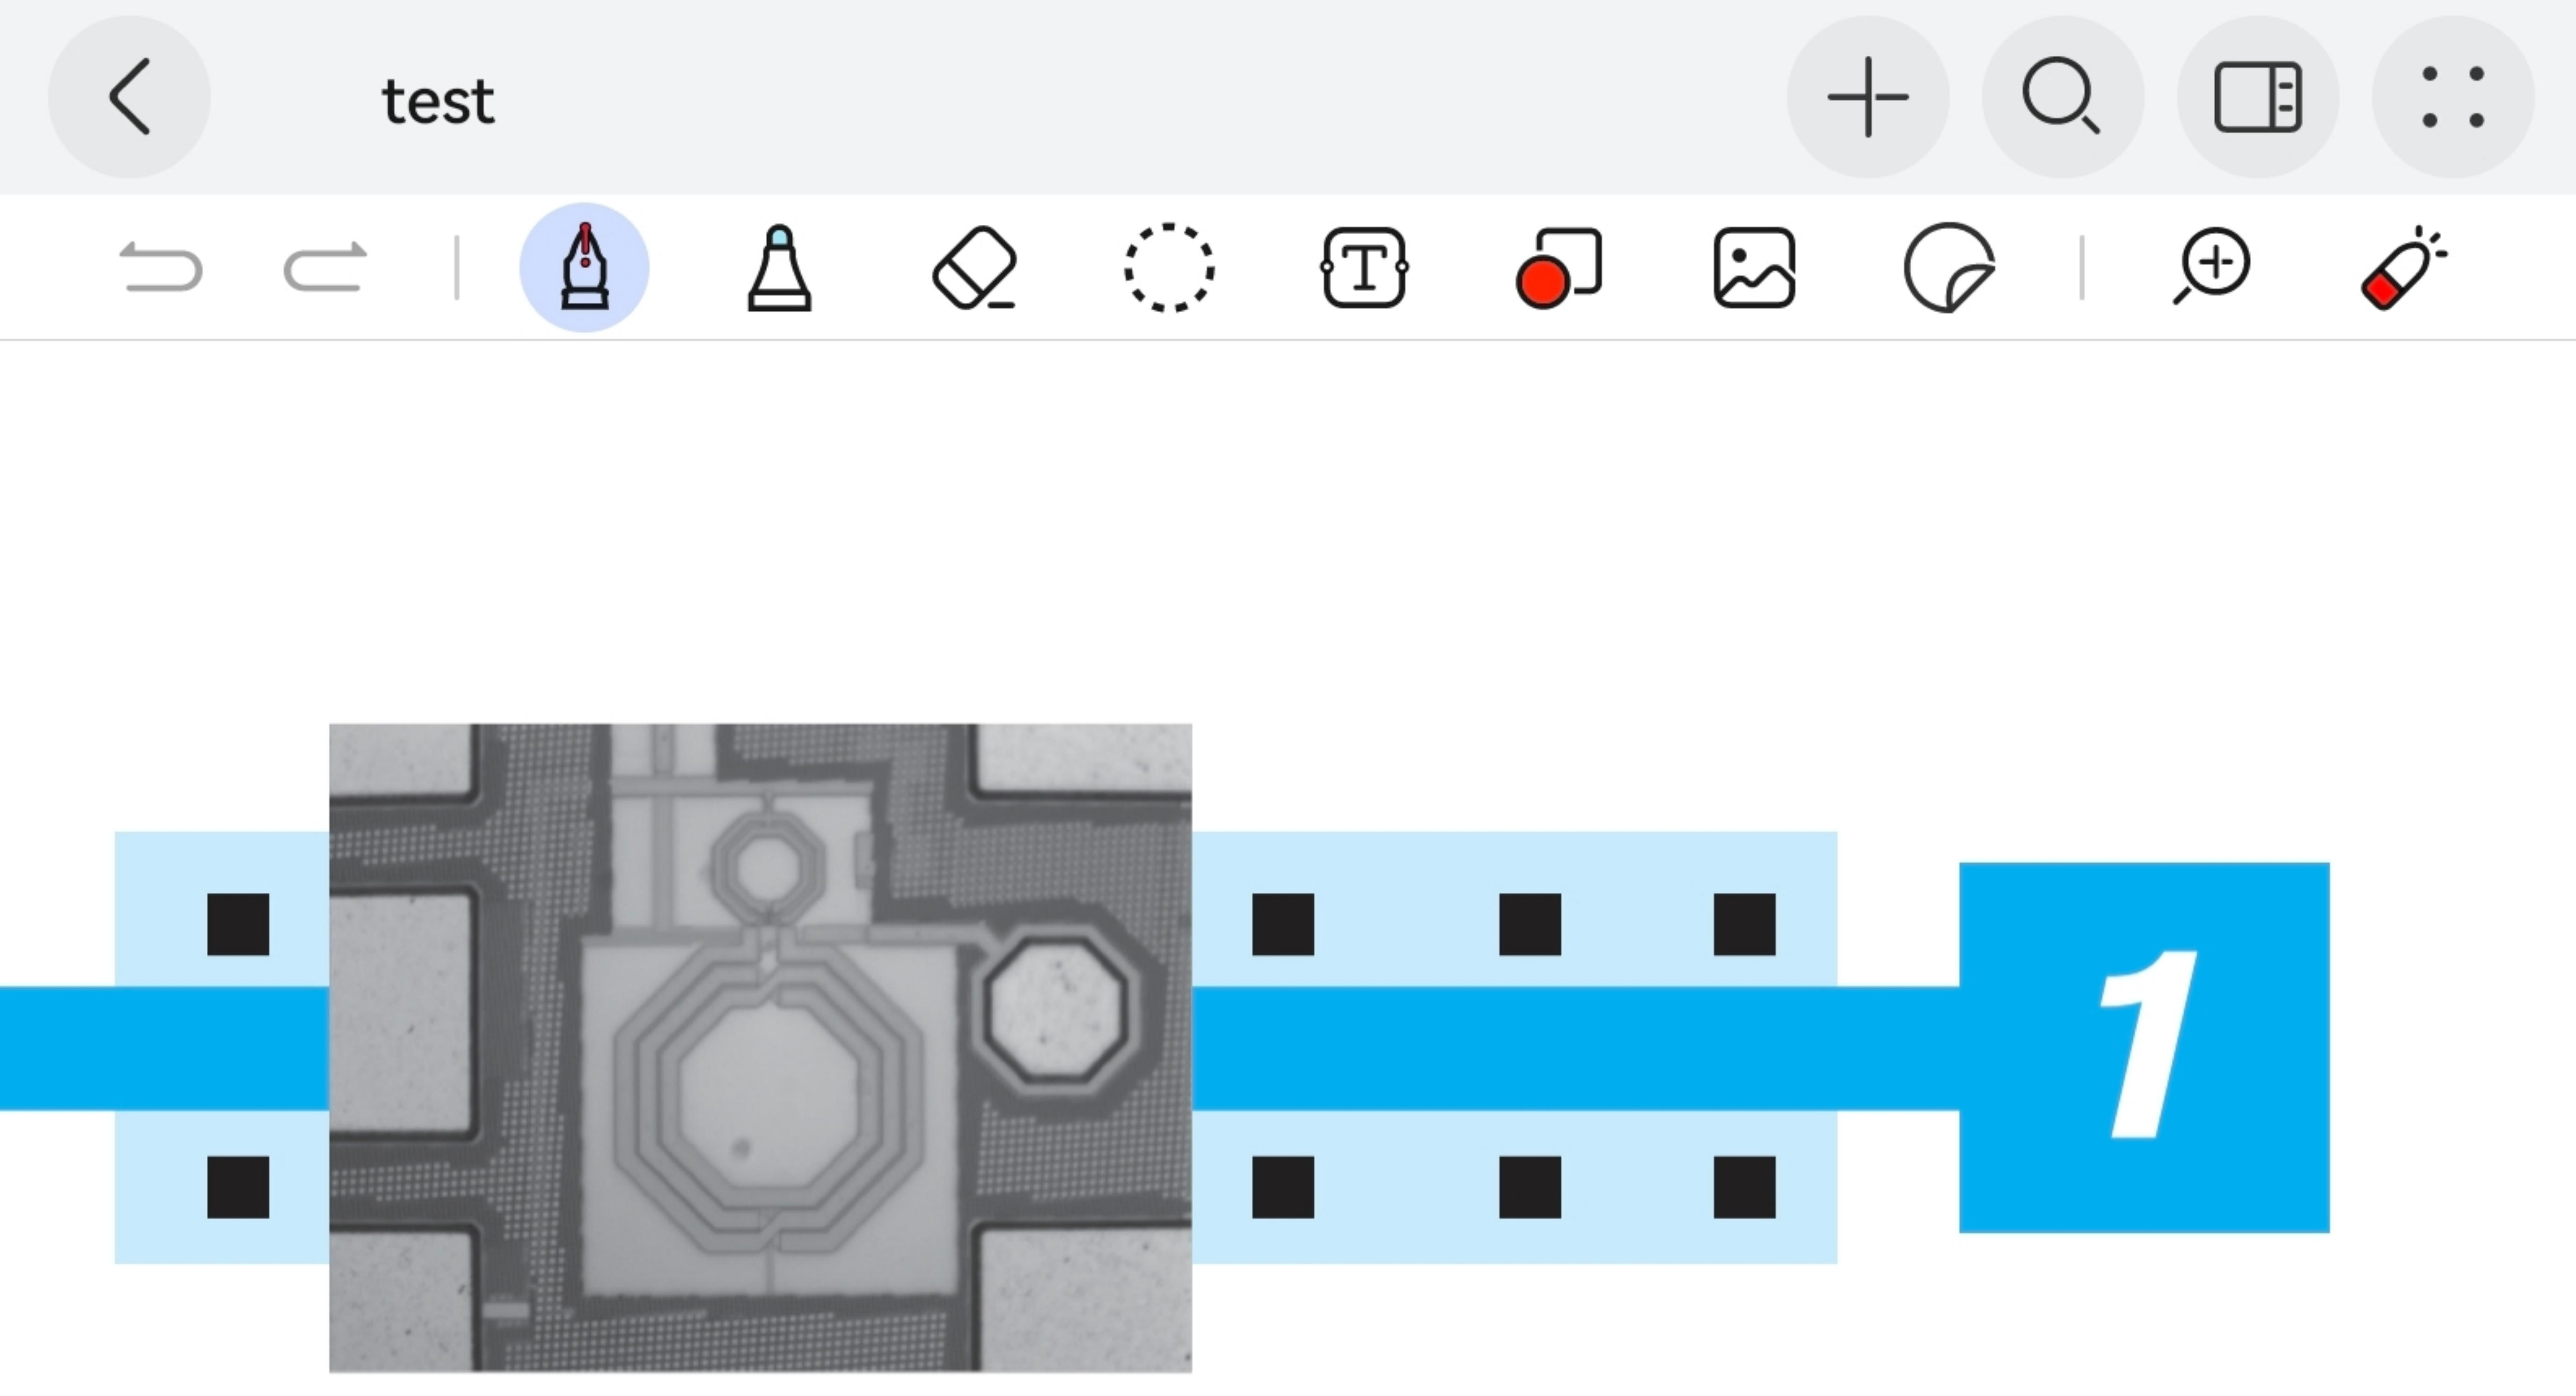
\includegraphics[max width=\textwidth]{2024_10_27_cec776a4495ed9df4dfcg-001}
\end{center}

Over the past five decades, microelectronics has revolutionized our lives. While beyond the realm of possibility a few decades ago, cellphones, digital cameras, laptop computers, and many other electronic products have now become an integral part of our daily affairs.

Learning microelectronics can be fun. As we learn how each device operates, how devices comprise circuits that perform interesting and useful functions, and how circuits form sophisticated systems, we begin to see the beauty of microelectronics and appreciate the reasons for its explosive growth.

This chapter gives an overview of microelectronics so as to provide a context for the material presented in this book. We introduce examples of microelectronic systems and identify important circuit "functions" that they employ. We also provide a review of basic circuit theory to refresh the reader's memory.

\subsection*{1.1 ELECTRONICS VERSUS MICROELECTRONICS}
The general area of electronics began about a century ago and proved instrumental in the radio and radar communications used during the two world wars. Early systems incorporated "vacuum tubes," amplifying devices that operated with the flow of electrons between plates in a vacuum chamber. However, the finite lifetime and the large size of vacuum tubes motivated researchers to seek an electronic device with better properties.

The first transistor was invented in the 1940s and rapidly displaced vacuum tubes. It exhibited a very long (in principle, infinite) lifetime and occupied a much smaller volume (e.g., less than $1 \mathrm{~cm}^{3}$ in packaged form) than vacuum tubes did.

But it was not until 1960s that the field of microelectronics, i.e., the science of integrating many transistors on one chip, began. Early "integrated circuits" (ICs) contained only a handful of devices, but advances in the technology soon made it possible to dramatically increase the complexity of "microchips."\\
\includegraphics[max width=\textwidth, center]{2024_10_27_cec776a4495ed9df4dfcg-002(1)}

\section*{2}
Chapter 1 Introduction to Microelectronics

\begin{center}
\begin{tabular}{|cl|}
\hline
Example & \begin{tabular}{l}
Today's microprocessors contain about 100 million transistors in a chip area of approx- \\
imately $3 \mathrm{~cm} \times 3 \mathrm{~cm}$. (The chip is a few hundred microns thick.) Suppose integrated \\
\end{tabular} \\
 & \begin{tabular}{l}
circuits were not invented and we attempted to build a processor using 100 million \\
\end{tabular} \\
 & \begin{tabular}{l}
"discrete" transistors. If each device occupies a volume of $3 \mathrm{~mm} \times 3 \mathrm{~mm} \times 3 \mathrm{~mm}$, de- \\
termine the minimum volume for the processor. What other issues would arise in such \\
an implementation? \\
\end{tabular} \\
\hline
\end{tabular}
\end{center}

Solution The minimum volume is given by $27 \mathrm{~mm}^{3} \times 10^{8}$, i.e., a cube 1.4 m on each side! Of course, the wires connecting the transistors would increase the volume substantially.

In addition to occupying a large volume, this discrete processor would be extremely slow; the signals would need to travel on wires as long as 1.4 m ! Furthermore, if each discrete transistor costs 1 cent and weighs 1 g , each processor unit would be priced at one million dollars and weigh 100 tons!

Exercise How much power would such a system consume if each transistor dissipates $10 \mu \mathrm{~W}$ ?

This book deals mostly with microelectronics while providing sufficient foundation for general (perhaps discrete) electronic systems as well.

\subsection*{1.2 EXAMPLES OF ELECTRONIC SYSTEMS}
At this point, we introduce two examples of microelectronic systems and identify some of the important building blocks that we should study in basic electronics.

\subsection*{1.2.1 Cellular Telephone}
Cellular telephones were developed in the 1980s and rapidly became popular in the 1990s. Today's cellphones contain a great deal of sophisticated analog and digital electronics that lie well beyond the scope of this book. But our objective here is to see how the concepts described in this book prove relevant to the operation of a cellphone.

Suppose you are speaking with a friend on your cellphone. Your voice is converted to an electric signal by a microphone and, after some processing, transmitted by the antenna. The signal produced by your antenna is picked up by your friend's receiver and, after some processing, applied to the speaker [Fig. 1.1(a)]. What goes on in these black boxes? Why are they needed?\\
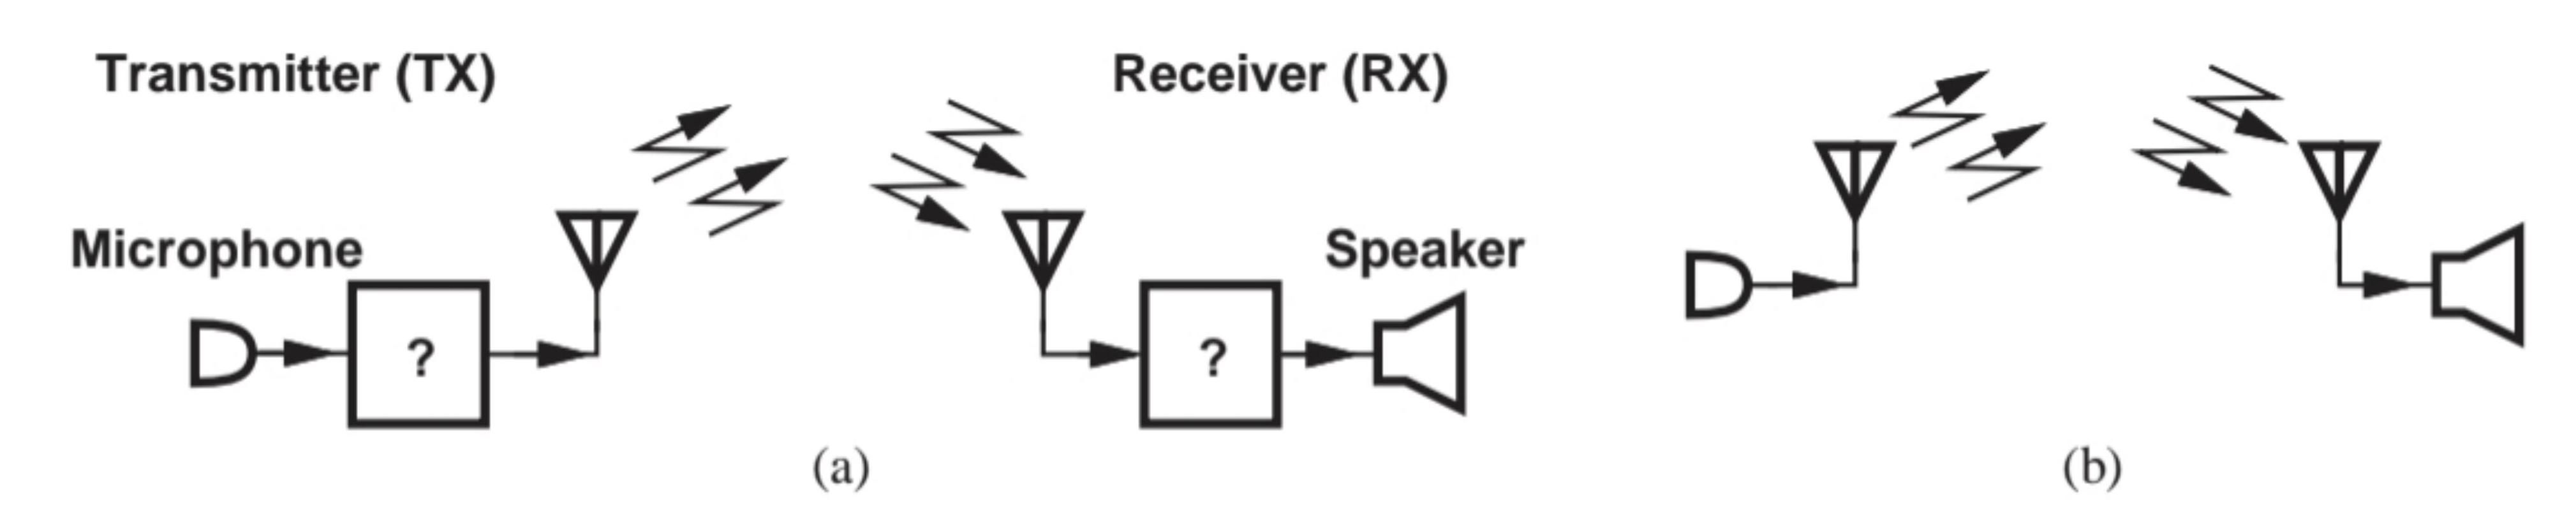
\includegraphics[max width=\textwidth, center]{2024_10_27_cec776a4495ed9df4dfcg-002}

Figure 1.1 (a) Simplified view of a cellphone, (b) further simplification of transmit and receive paths.\\
\includegraphics[max width=\textwidth, center]{2024_10_27_cec776a4495ed9df4dfcg-003}

Let us attempt to omit the black boxes and construct the simple system shown in Fig. 1.1(b). How well does this system work? We make two observations. First, our voice contains frequencies from 20 Hz to 20 kHz (called the "voice band"). Second, for an antenna to operate efficiently, i.e., to convert most of the electrical signal to electromagnetic radiation, its dimension must be a significant fraction (e.g., $25 \%$ ) of the wavelength. Unfortunately, a frequency range of 20 Hz to 20 kHz translates to a wavelength ${ }^{1}$ of $1.5 \times 10^{7}$ m to $1.5 \times 10^{4} \mathrm{~m}$, requiring gigantic antennas for each cellphone. Conversely, to obtain a reasonable antenna length, e.g., 5 cm , the wavelength must be around 20 cm and the frequency around 1.5 GHz .

How do we "convert" the voice band to a gigahertz center frequency? One possible approach is to multiply the voice signal, $x(t)$, by a sinusoid, $A \cos \left(2 \pi f_{c} t\right)[$ Fig. 1.2(a)]. Since multiplication in the time domain corresponds to convolution in the frequency domain, and since the spectrum of the sinusoid consists of two impulses at $\pm f_{c}$, the voice spectrum is simply shifted (translated) to $\pm f_{c}$ [Fig. 1.2(b)]. Thus, if $f_{c}=1 \mathrm{GHz}$, the output occupies a bandwidth of 40 kHz centered at 1 GHz . This operation is an example of "amplitude modulation." 2\\
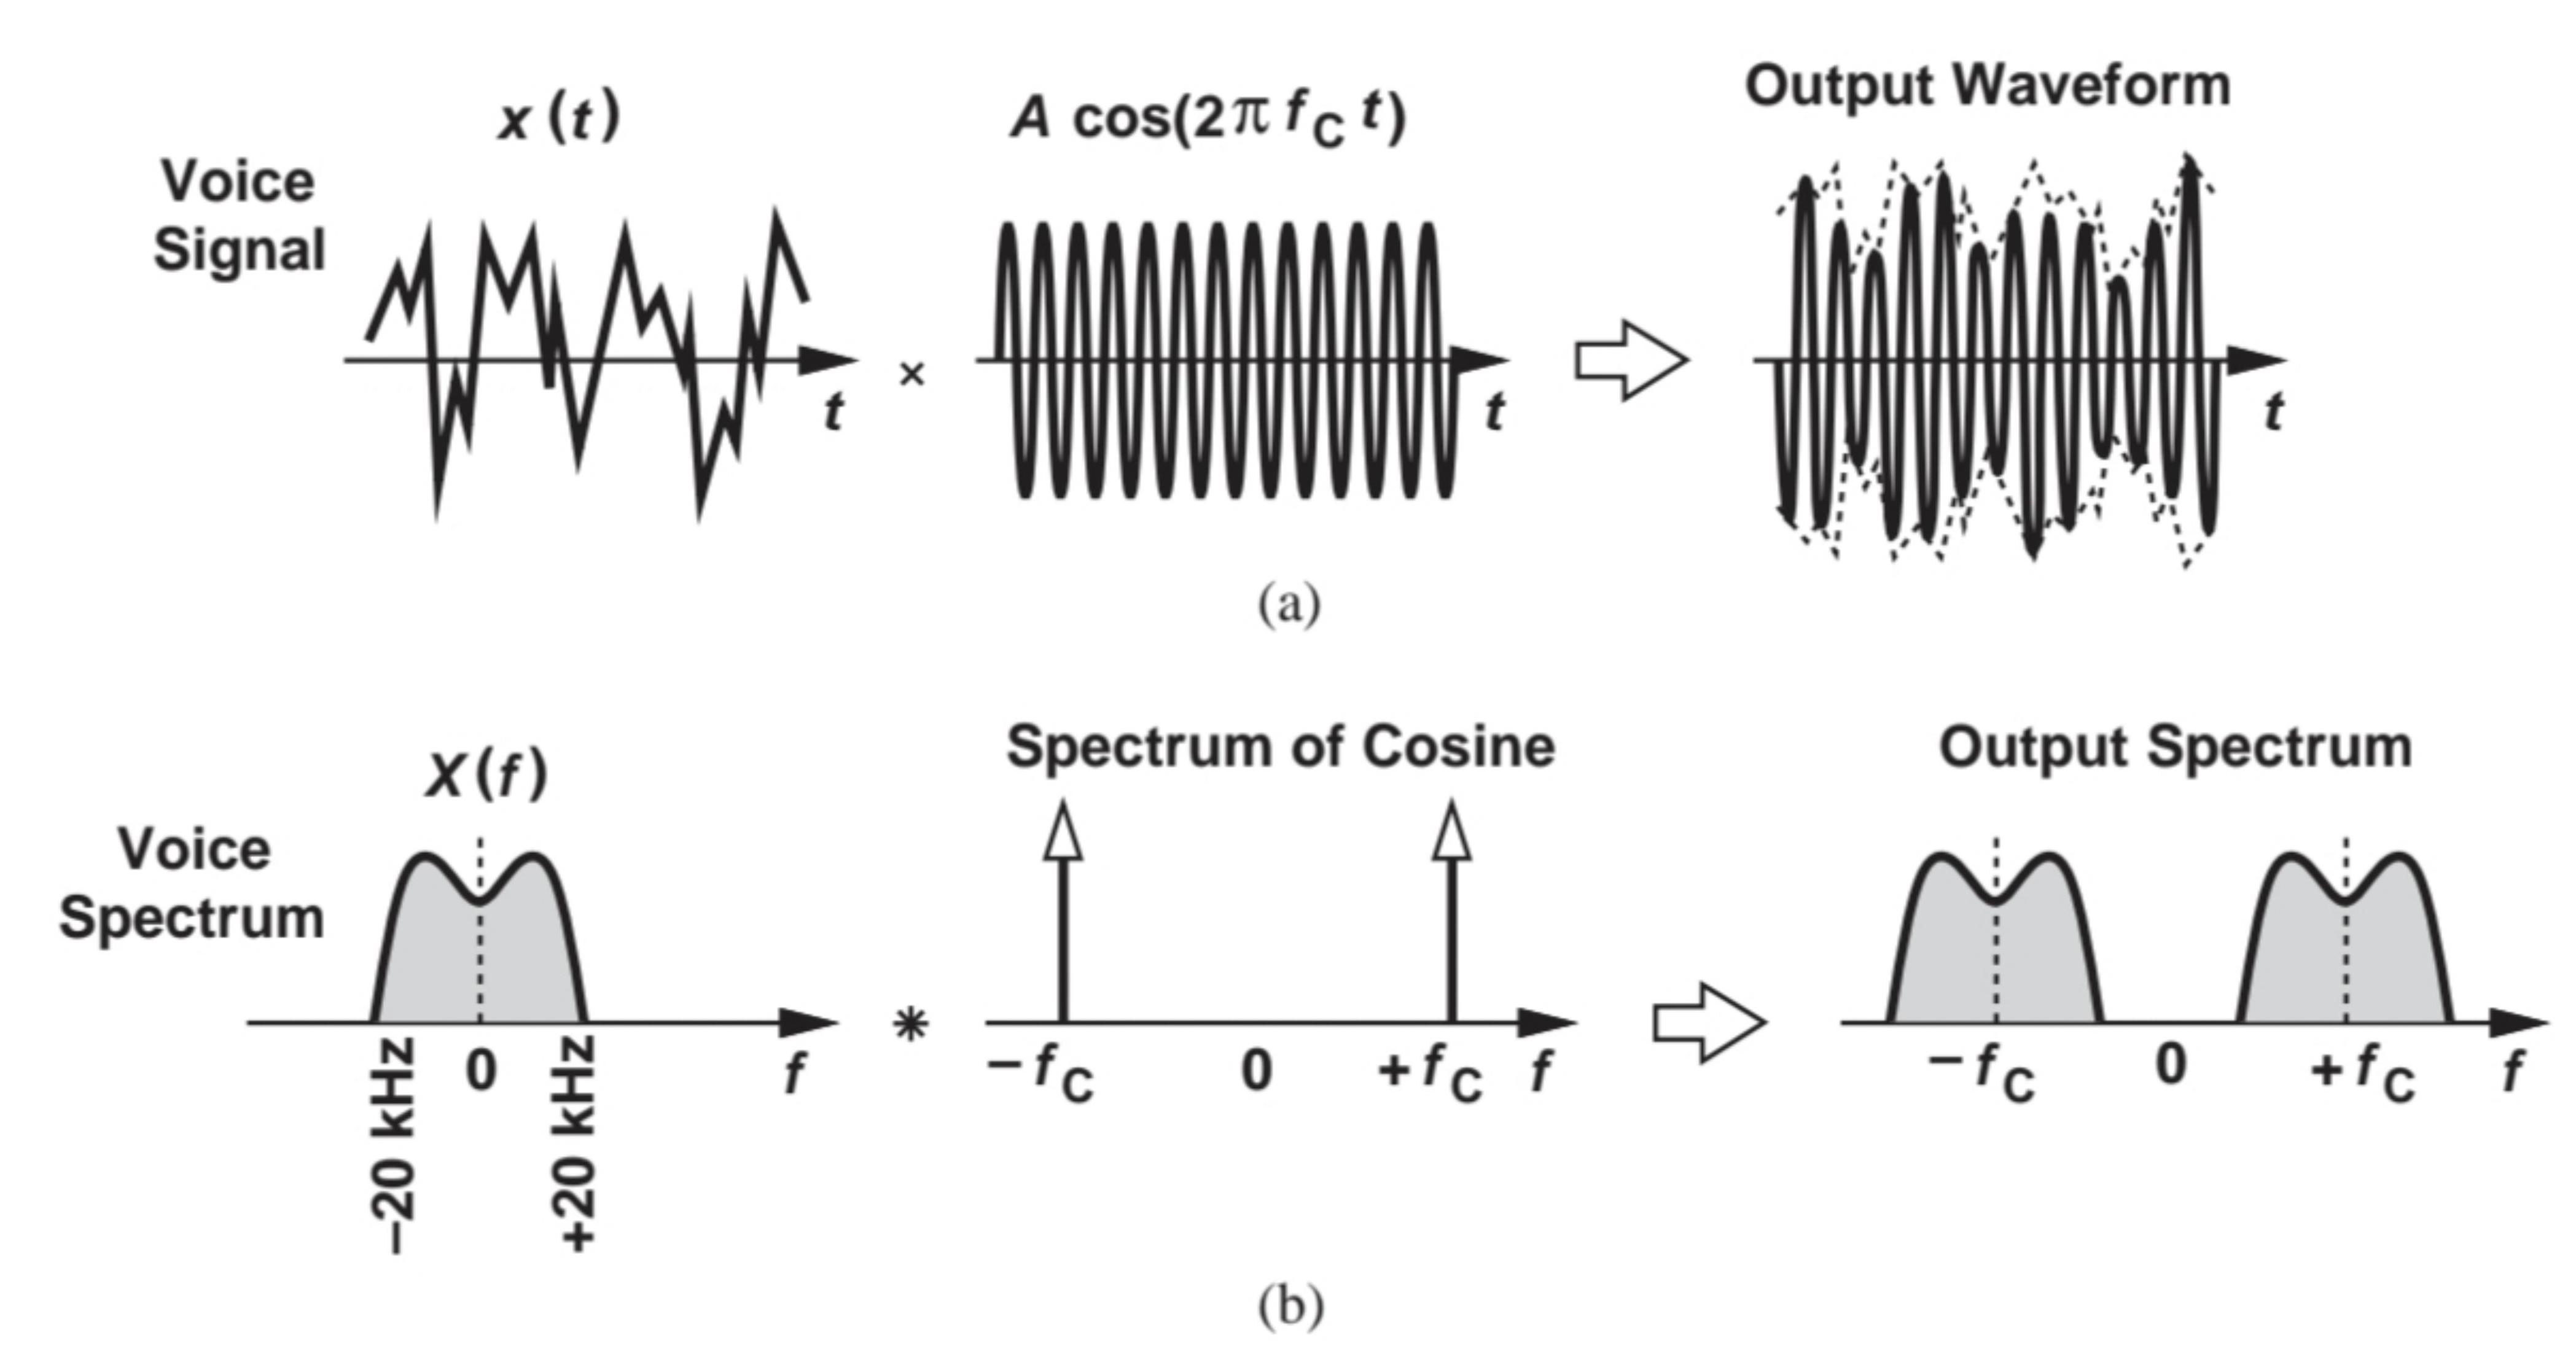
\includegraphics[max width=\textwidth, center]{2024_10_27_cec776a4495ed9df4dfcg-003(1)}

Figure 1.2 (a) Multiplication of a voice signal by a sinusoid, (b) equivalent operation in the frequency domain.

We therefore postulate that the black box in the transmitter of Fig. 1.1(a) contains a multiplier, ${ }^{3}$ as depicted in Fig. 1.3(a). But two other issues arise. First, the cellphone must deliver a relatively large voltage swing (e.g., $20 \mathrm{~V}_{p p}$ ) to the antenna so that the radiated power can reach across distances of several kilometers, thereby requiring a "power amplifier" between the multiplier and the antenna. Second, the sinusoid, $A \cos 2 \pi f_{c} t$, must be produced by an "oscillator." We thus arrive at the transmitter architecture shown in Fig. 1.3(b).

\footnotetext{${ }^{1}$ Recall that the wavelength is equal to the (light) velocity divided by the frequency.\\
${ }^{2}$ Cellphones in fact use other types of modulation to translate the voice band to higher frequencies.\\
${ }^{3}$ Also called a "mixer" in high-frequen
}
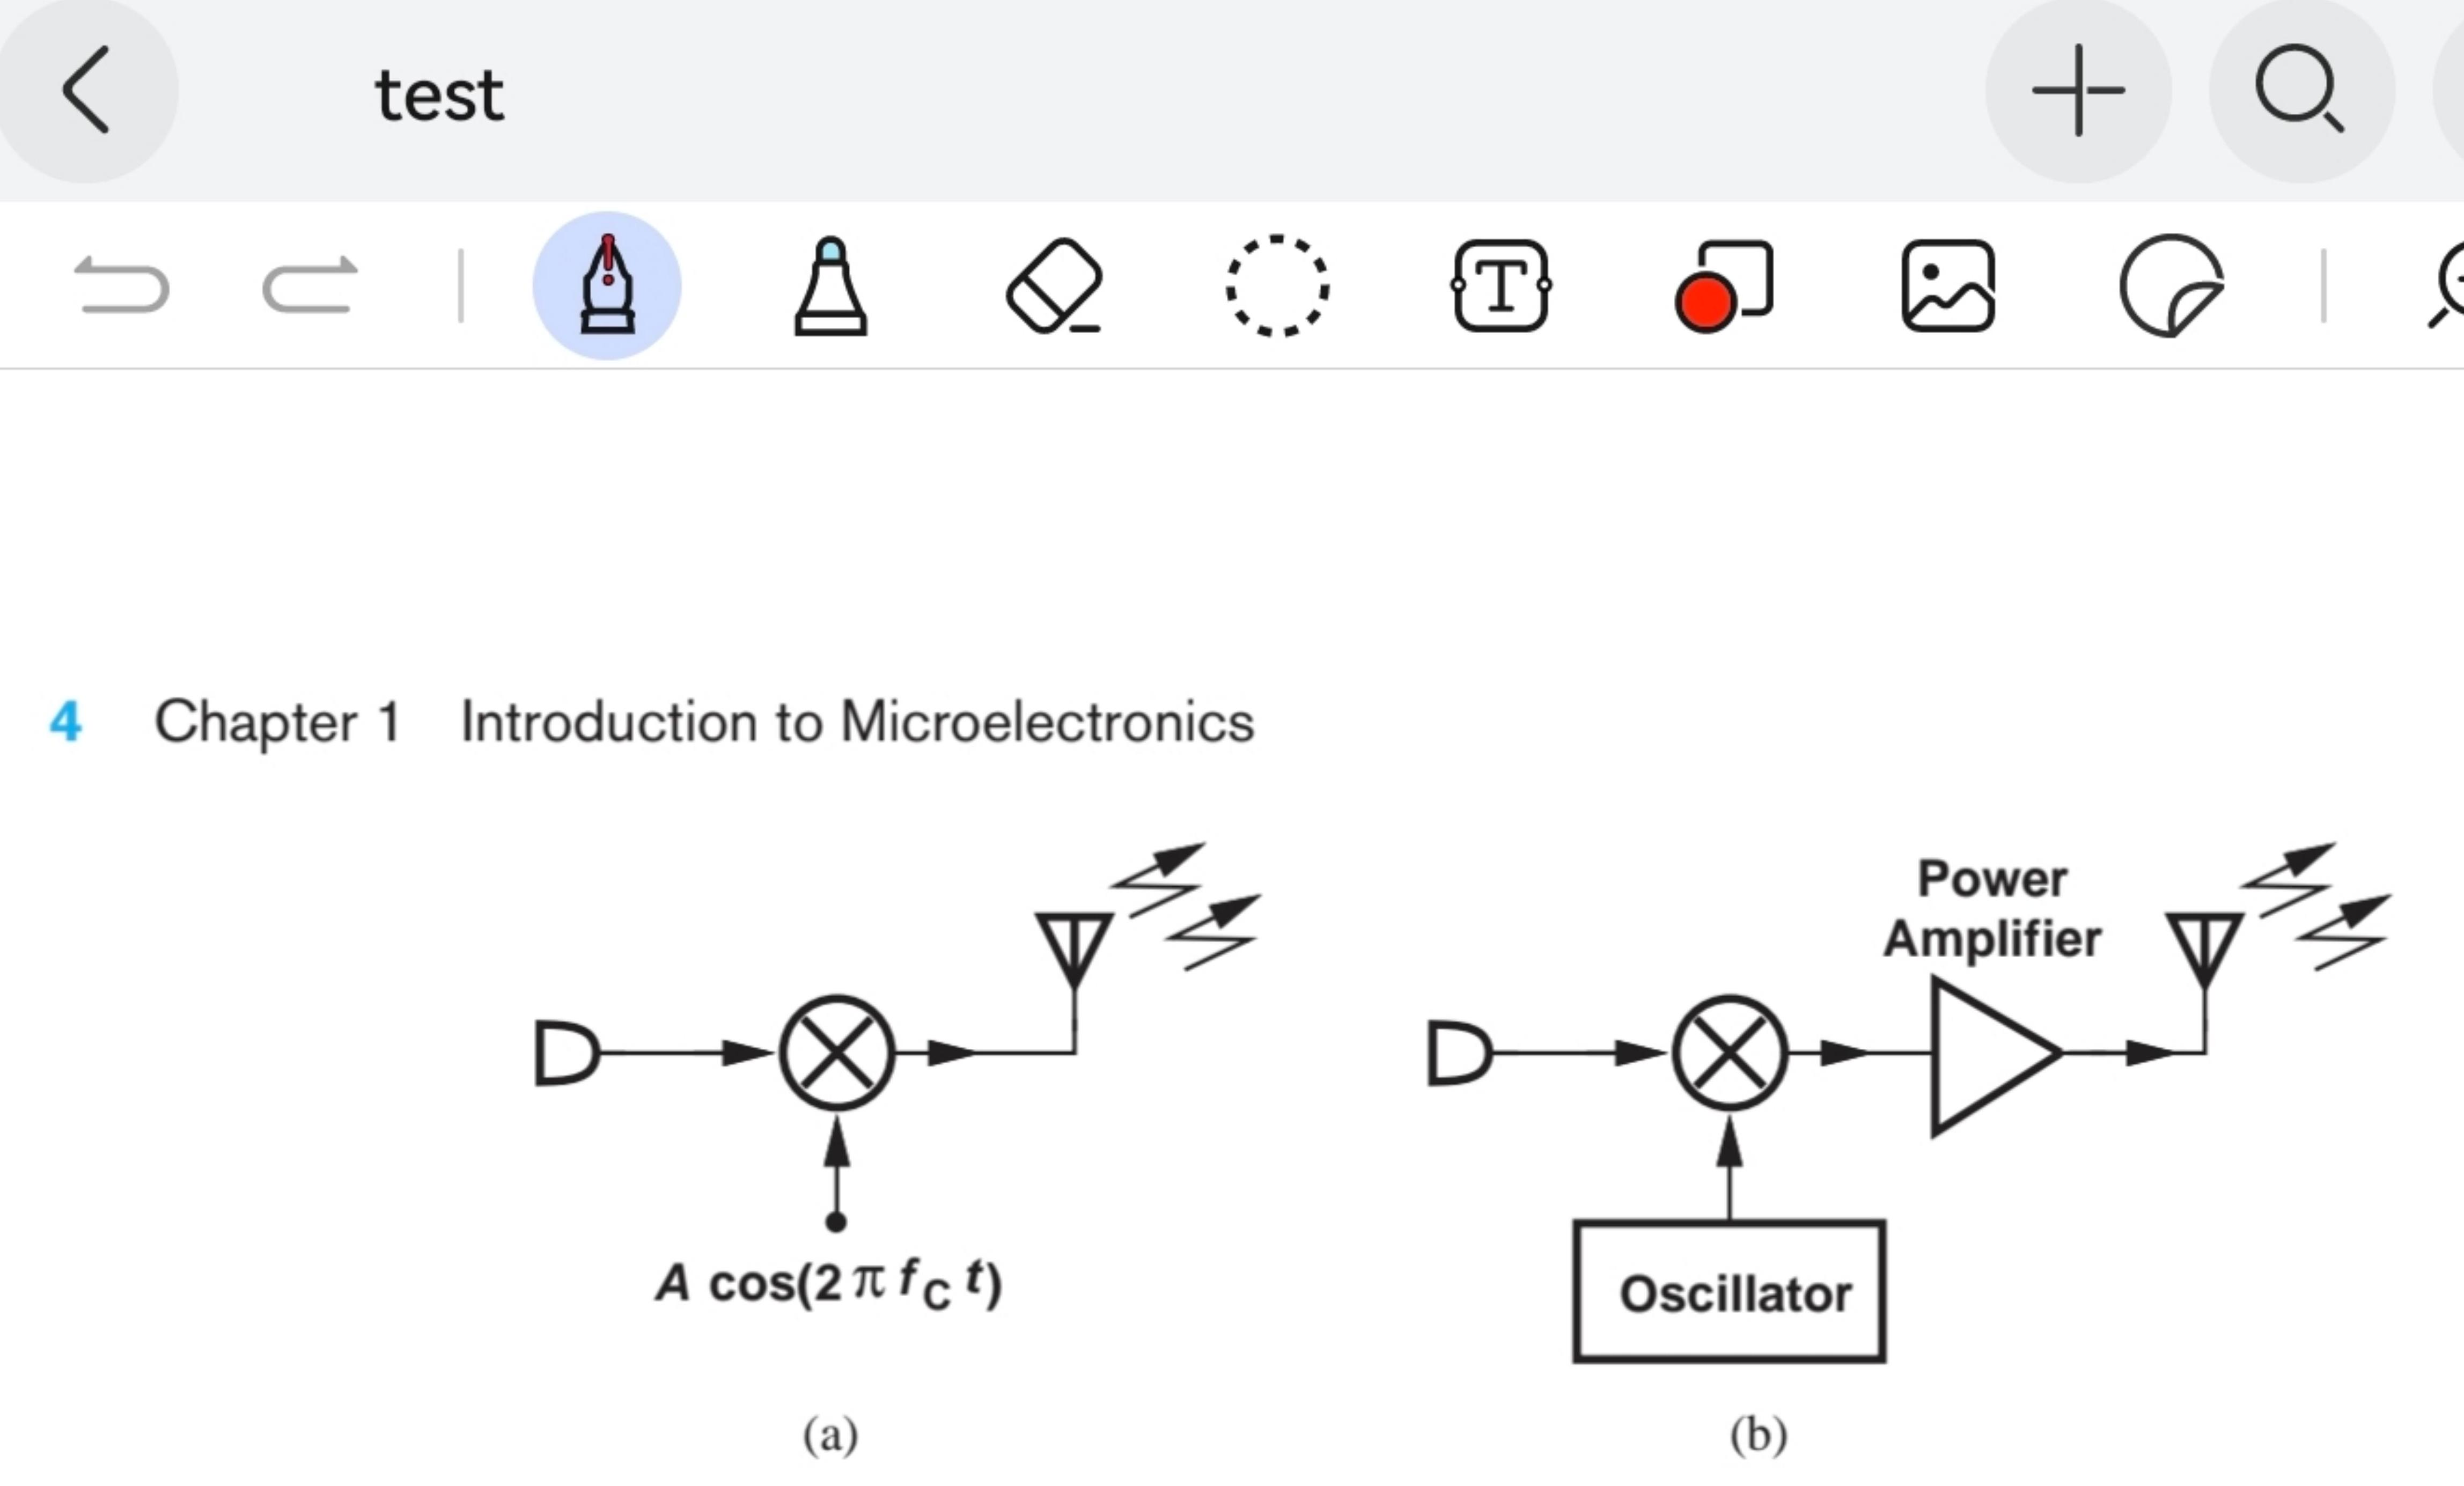
\includegraphics[max width=\textwidth, center]{2024_10_27_cec776a4495ed9df4dfcg-004(1)}

Figure 1.3 (a) Simple transmitter, (b) more complete transmitter.

Let us now turn our attention to the receive path of the cellphone, beginning with the simple realization illustrated in Fig. 1.1(b). Unfortunately, this topology fails to operate with the principle of modulation: if the signal received by the antenna resides around a gigahertz center frequency, the audio speaker cannot produce meaningful information. In other words, a means of translating the spectrum back to zero center frequency is necessary. For example, as depicted in Fig. 1.4(a), multiplication by a sinusoid, $A \cos \left(2 \pi f_{c} t\right)$, translates the spectrum to left and right by $f_{c}$, restoring the original voice band. The newly-generated components at $\pm 2 f_{c}$ can be removed by a low-pass filter. We thus arrive at the receiver topology shown in Fig. 1.4(b).\\
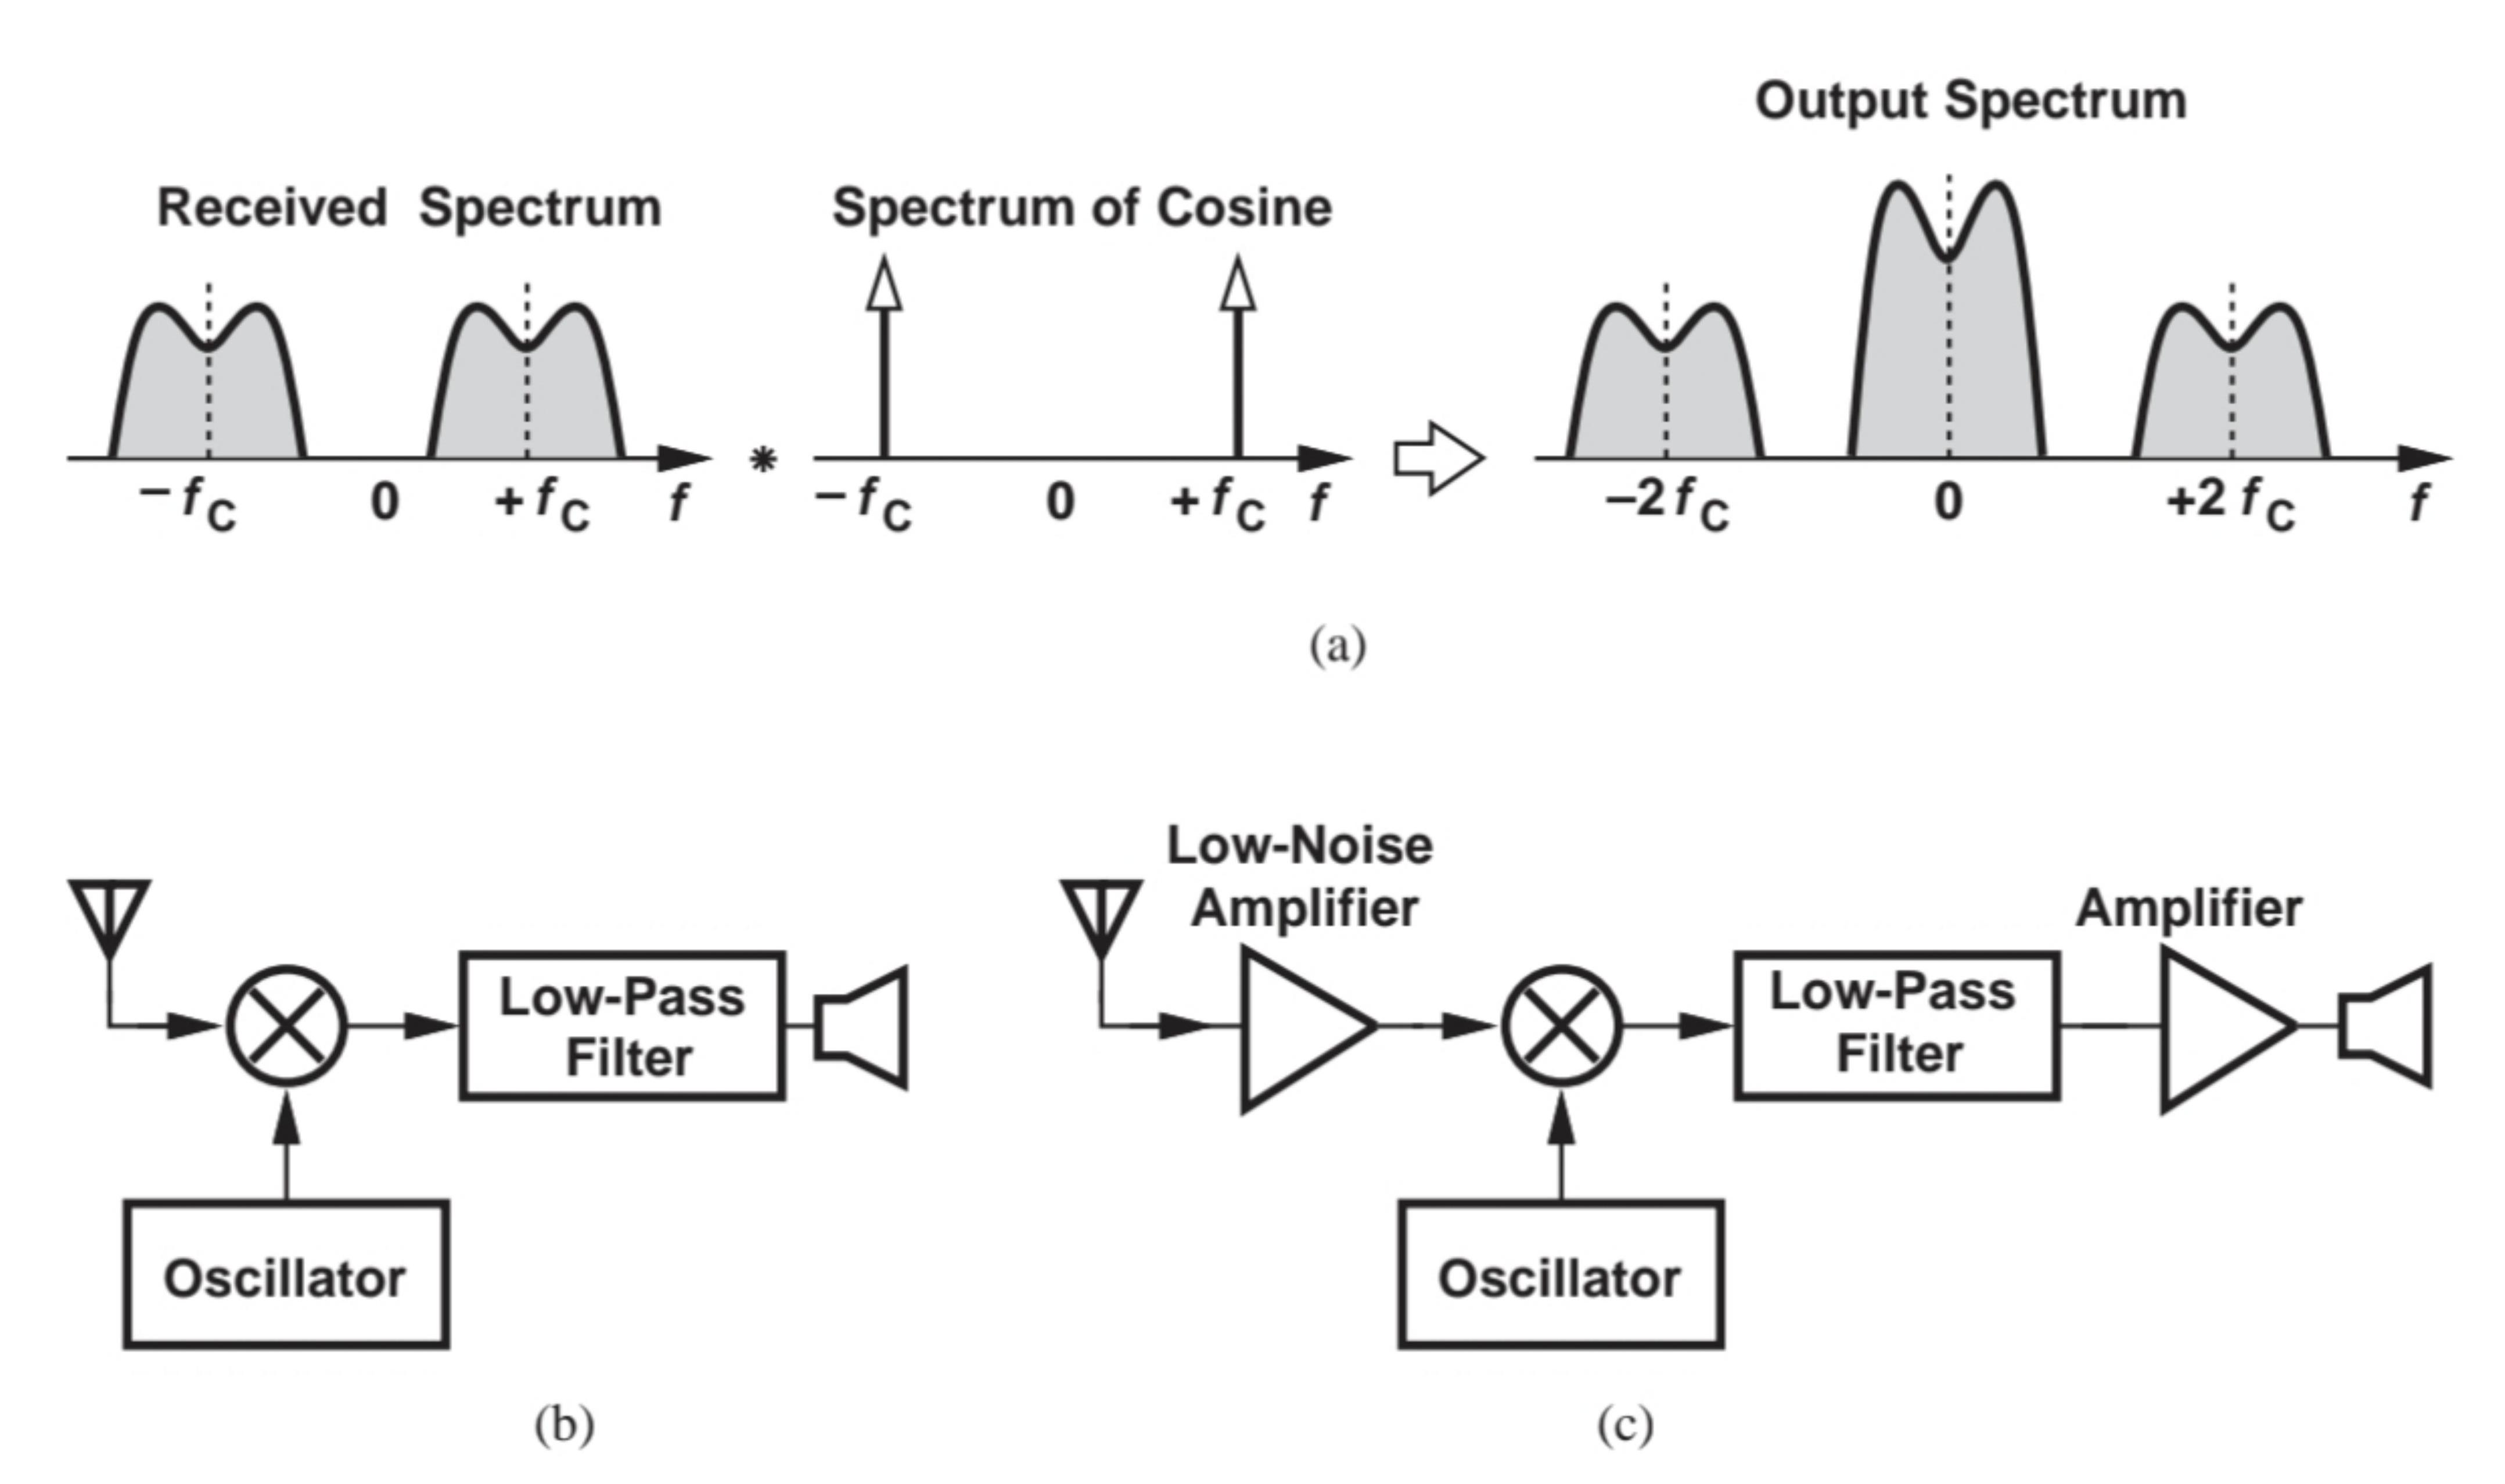
\includegraphics[max width=\textwidth, center]{2024_10_27_cec776a4495ed9df4dfcg-004}

Figure 1.4 (a) Translation of modulated signal to zero center frequency, (b) simple receiver, (b) more complete receiver.

Our receiver design is still incomplete. The signal received by the antenna can be as low as a few tens of microvolts whereas the speaker may require swings of several tens\\
\includegraphics[max width=\textwidth, center]{2024_10_27_cec776a4495ed9df4dfcg-005}\\
1.2 Examples of Electronic Systems

5\\
or hundreds of millivolts. That is, the receiver must provide a great deal of amplification ("gain") between the antenna and the speaker. Furthermore, since multipliers typically suffer from a high "noise" and hence corrupt the received signal, a "low-noise amplifier" must precede the multiplier. The overall architecture is depicted in Fig. 1.4(c).

Today's cellphones are much more sophisticated than the topologies developed above. For example, the voice signal in the transmitter and the receiver is applied to a digital signal processor (DSP) to improve the quality and efficiency of the communication. Nonetheless, our study reveals some of the fundamental building blocks of cellphones, e.g., amplifiers, oscillators, and filters, with the last two also utilizing amplification. We therefore devote a great deal of effort to the analysis and design of amplifiers.

Having seen the necessity of amplifiers, oscillators, and multipliers in both transmit and receive paths of a cellphone, the reader may wonder if "this is old stuff" and rather trivial compared to the state of the art. Interestingly, these building blocks still remain among the most challenging circuits in communication systems. This is because the design entails critical trade-offs between speed (gigahertz center frequencies), noise, power dissipation (i.e., battery lifetime), weight, cost (i.e., price of a cellphone), and many other parameters. In the competitive world of cellphone manufacturing, a given design is never "good enough" and the engineers are forced to further push the above trade-offs in each new generation of the product.

\subsection*{1.2.2 Digital Camera}
Another consumer product that, by virtue of "going electronic," has dramatically changed our habits and routines is the digital camera. With traditional cameras, we received no immediate feedback on the quality of the picture that was taken, we were very careful in selecting and shooting scenes to avoid wasting frames, we needed to carry bulky rolls of film, and we would obtain the final result only in printed form. With digital cameras, on the other hand, we have resolved these issues and enjoy many other features that only electronic processing can provide, e.g., transmission of pictures through cellphones or ability to retouch or alter pictures by computers. In this section, we study the operation of the digital camera.

The "front end" of the camera must convert light to electricity, a task performed by an array (matrix) of "pixels." ${ }^{4}$ Each pixel consists of an electronic device (a "photodiode") that produces a current proportional to the intensity of the light that it receives. As illustrated in Fig. 1.5(a), this current flows through a capacitance, $C_{L}$, for a certain period of time, thereby developing a proportional voltage across it. Each pixel thus provides a voltage proportional to the "local" light density.

Now consider a camera with, say, 6.25 million pixels arranged in a $2500 \times 2500$ array [Fig. 1.5(b)]. How is the output voltage of each pixel sensed and processed? If each pixel contains its own electronic circuitry, the overall array occupies a very large area, raising the cost and the power dissipation considerably. We must therefore "time-share" the signal processing circuits among pixels. To this end, we follow the circuit of Fig. 1.5(a) with a simple, compact amplifier and a switch (within the pixel) [Fig. 1.5(c)]. Now, we connect a wire to the outputs of all 2500 pixels in a "column," turn on only one switch at a time, and apply the corresponding voltage to the "signal processing" block outside the column.\\
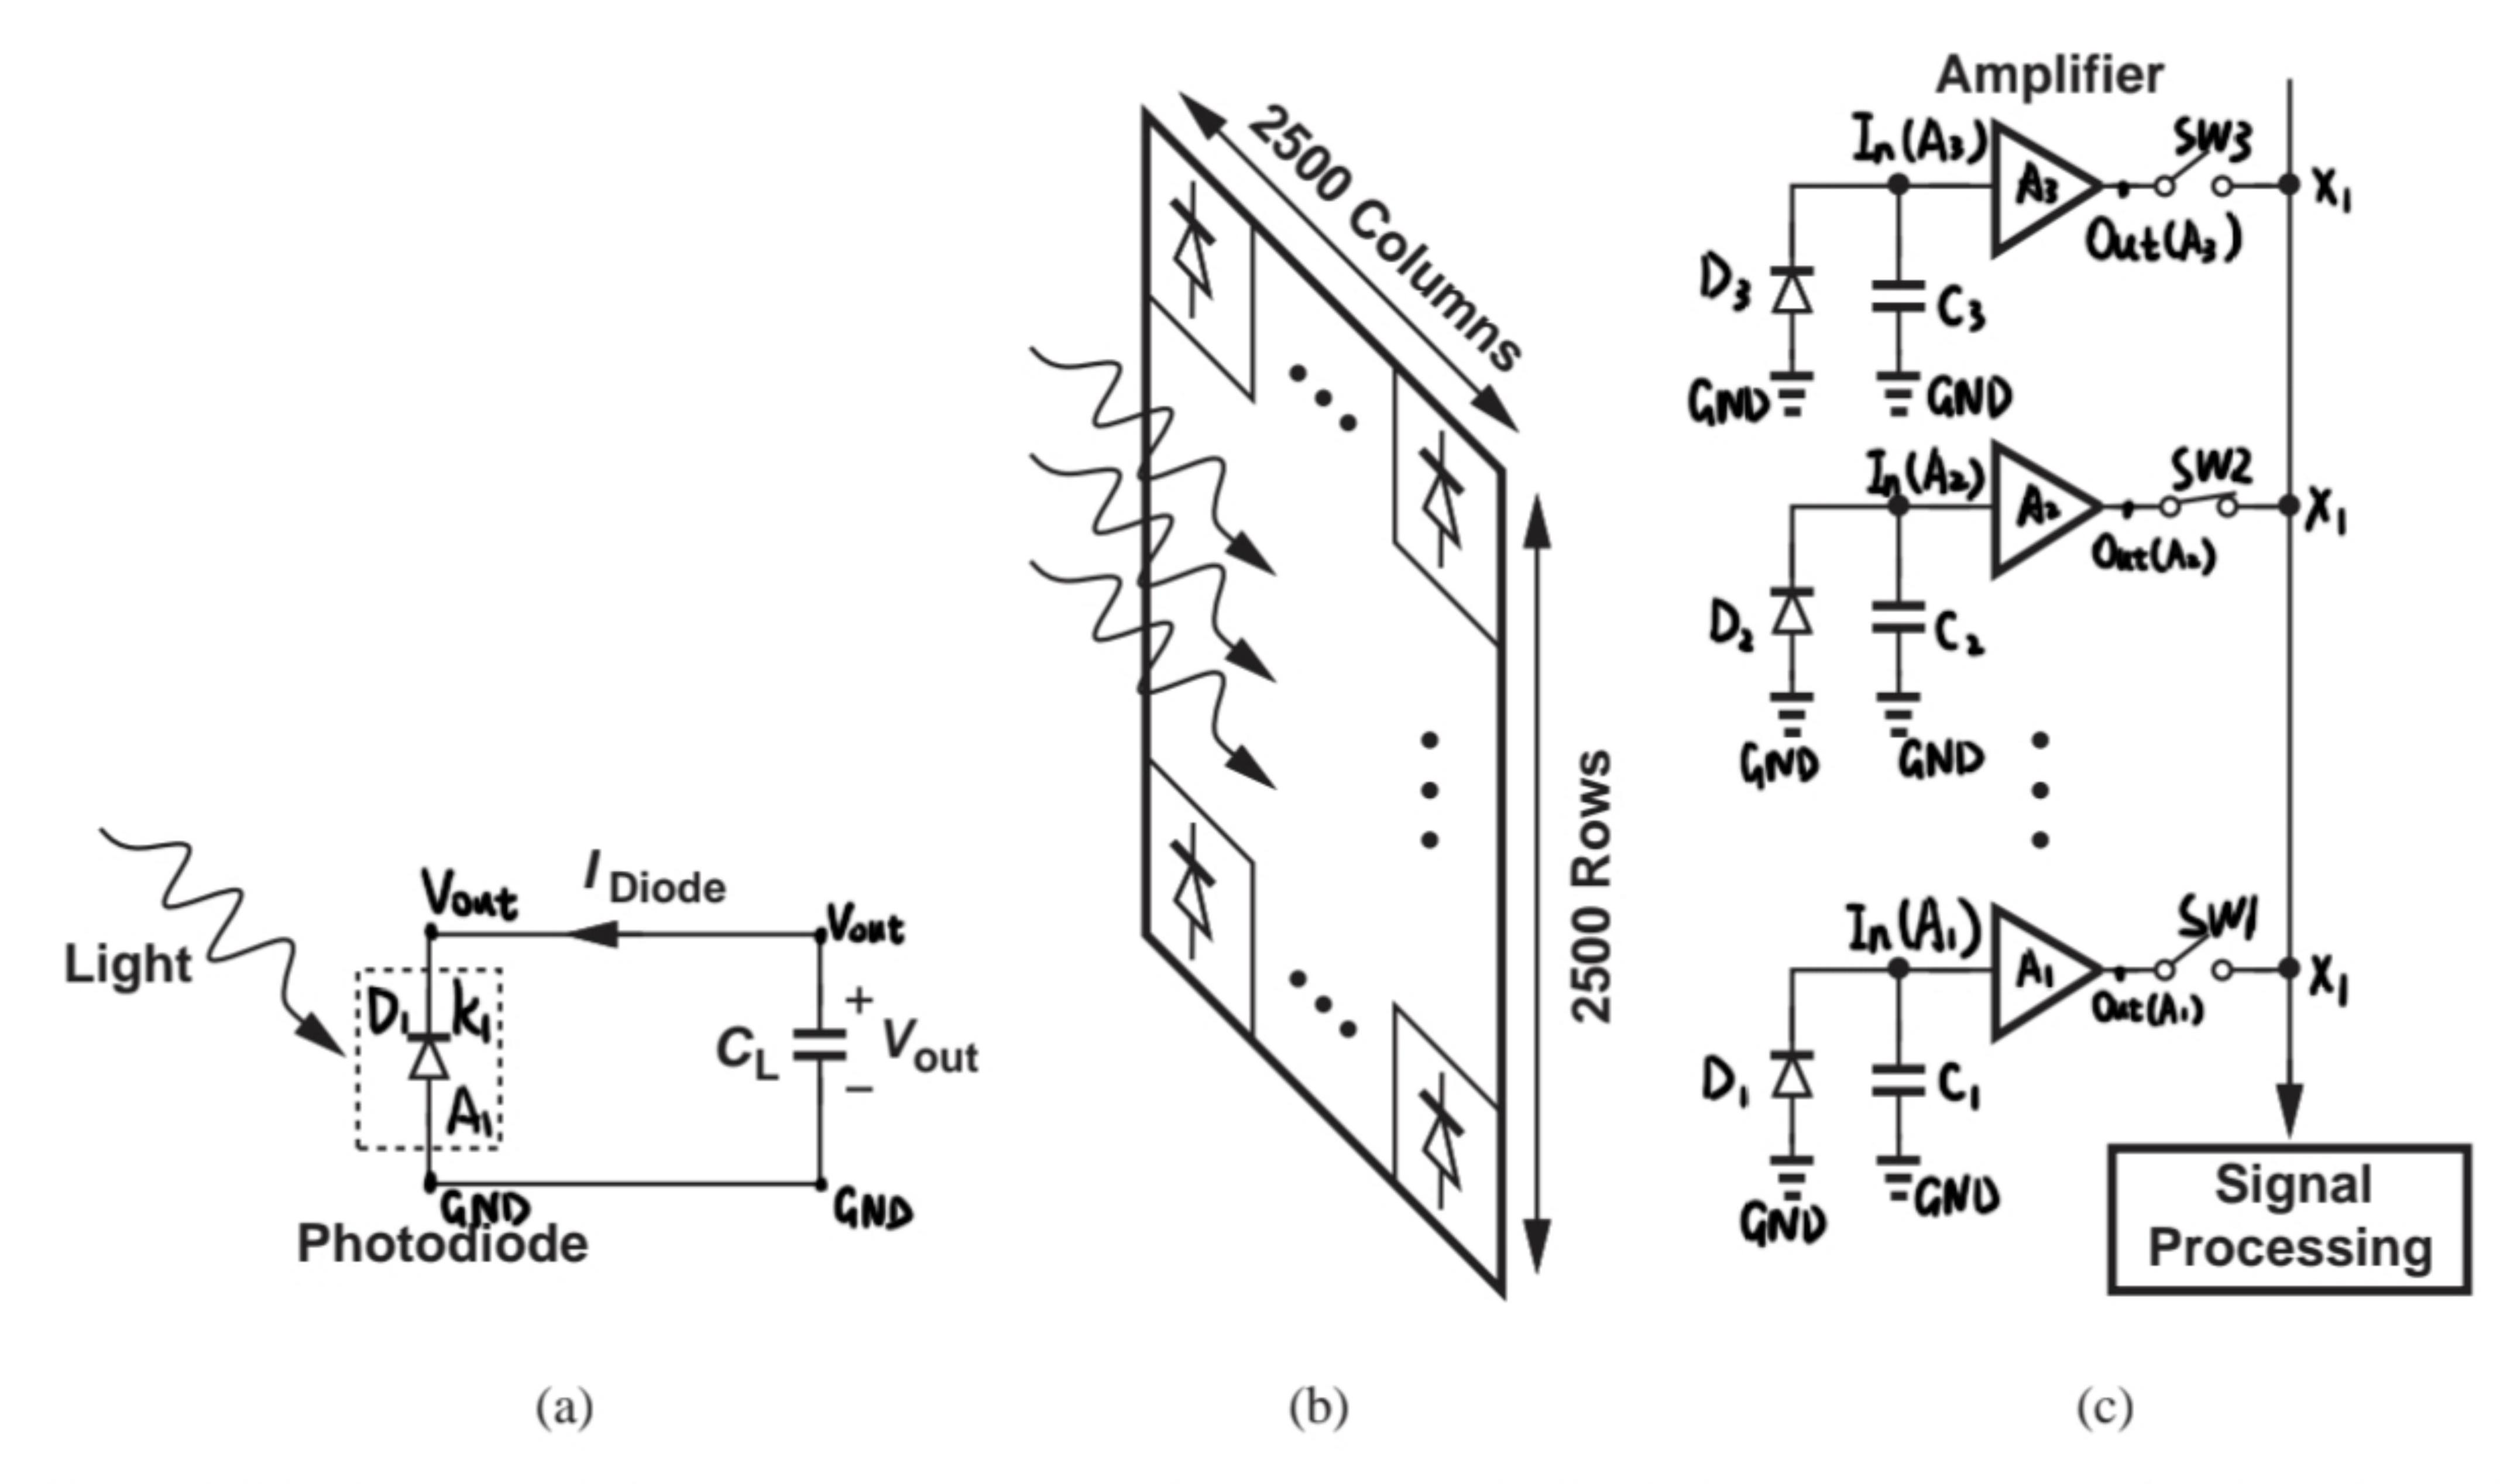
\includegraphics[max width=\textwidth, center]{2024_10_27_cec776a4495ed9df4dfcg-006(1)}

Figure 1.5 (a) Operation of a photodiode, (b) array of pixels in a digital camera, (c) one column of the array.

The overall array consists of 2500 of such columns, with each column employing a dedicated signal processing block.

Example\\
1.2

\section*{Solution}
A digital camera is focused on a chess board. Sketch the voltage produced by one column as a function of time.

The pixels in each column receive light only from the white squares [Fig. 1.6(a)]. Thus, the column voltage alternates between a maximum for such pixels and zero for those receiving no light. The resulting waveform is shown in Fig. 1.6(b).\\
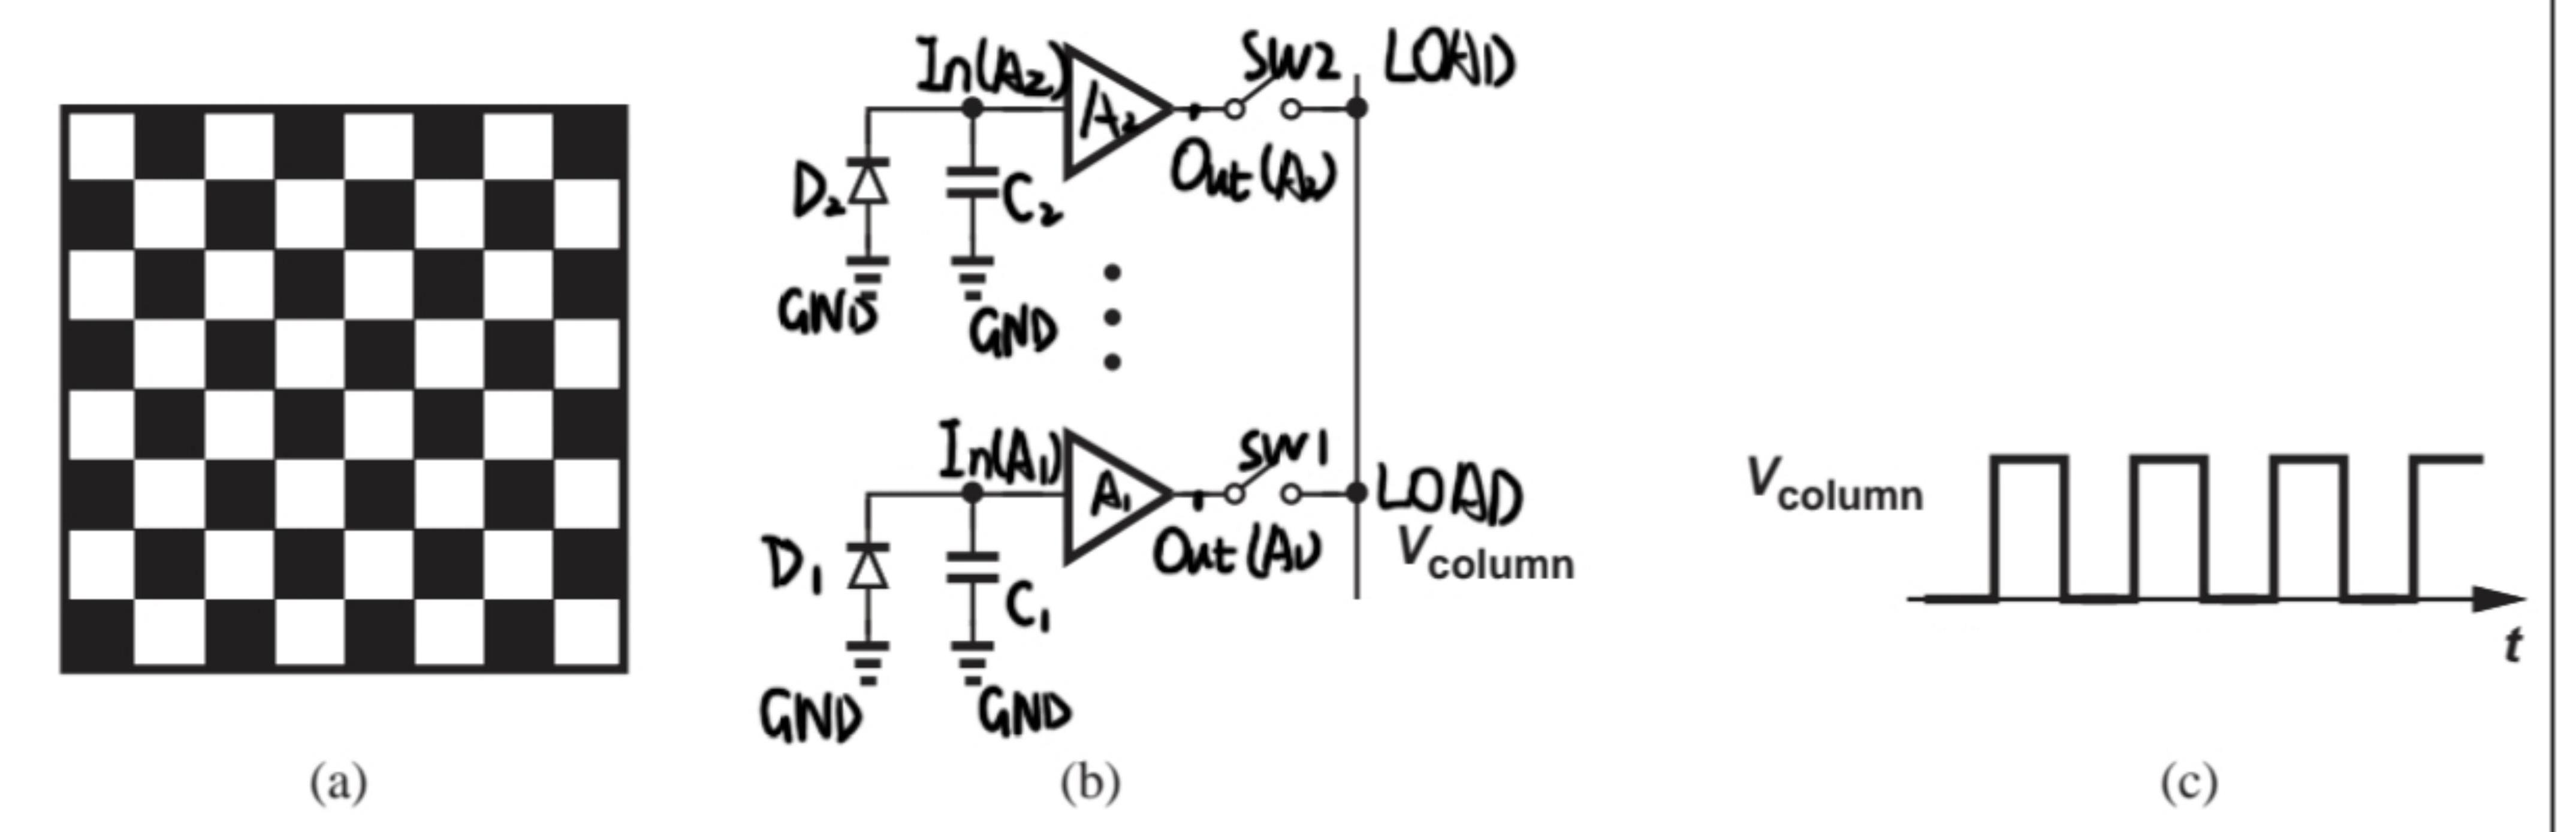
\includegraphics[max width=\textwidth, center]{2024_10_27_cec776a4495ed9df4dfcg-006}

Figure 1.6 (a) Chess board captured by a digital camera, (b) voltage waveform of one column.

\footnotetext{Exercise\\
Plot the voltage if the first and second squares in each row have the same color.
}What does each signal processing block do? Since the voltage produced by each pixel is an analog signal and can assume all values within a range, we must first "digitize" it by means of an "analog-to-digital converter" (ADC). A 6.25 megapixel array must thus incorporate 2500 ADCs. Since ADCs are relatively complex circuits, we may time-share one ADC between every two columns (Fig. 1.7), but requiring that the ADC operate twice as fast (why?). In the extreme case, we may employ a single, very fast ADC for all 2500 columns. In practice, the optimum choice lies between these two extremes.\\
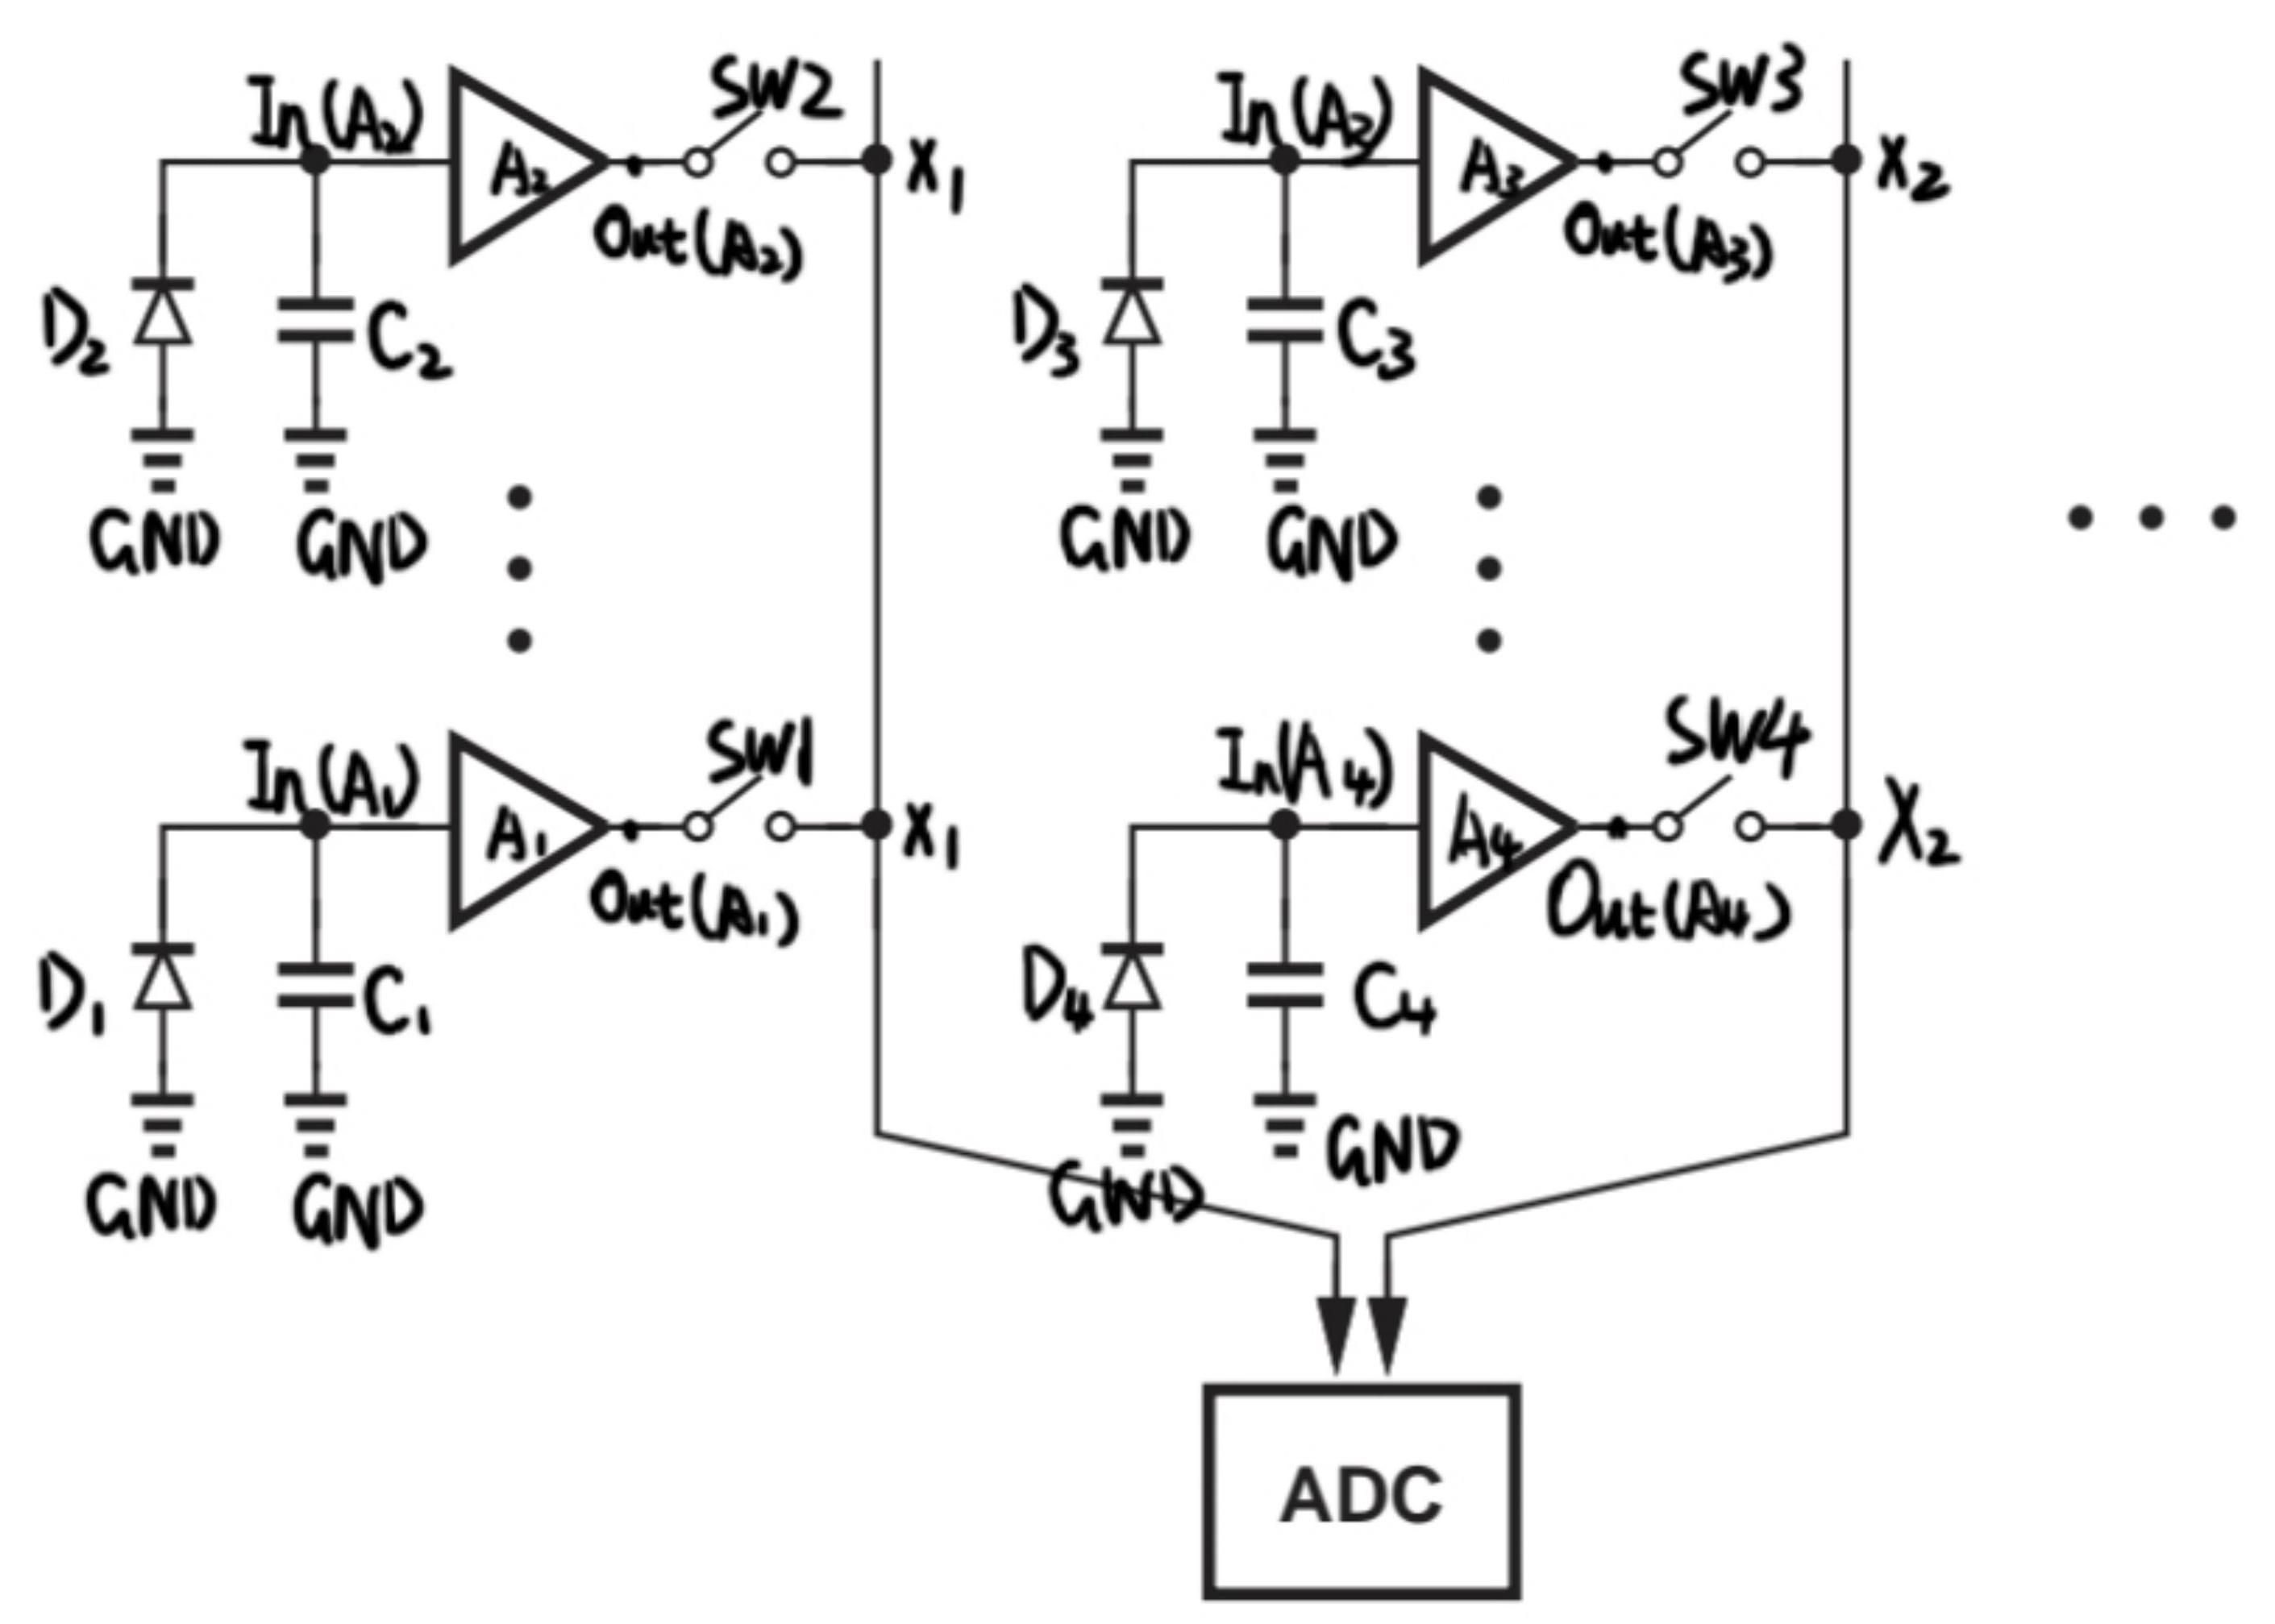
\includegraphics[max width=\textwidth, center]{2024_10_27_cec776a4495ed9df4dfcg-007}

Figure 1.7 Sharing one ADC between two columns of a pixel array.

Once in the digital domain, the "video" signal collected by the camera can be manipulated extensively. For example, to "zoom in," the digital signal processor (DSP) simply considers only a section of the array, discarding the information from the remaining pixels. Also, to reduce the required memory size, the processor "compresses" the video signal.

The digital camera exemplifies the extensive use of both analog and digital microelectronics. The analog functions include amplification, switching operations, and analog-todigital conversion, and the digital functions consist of subsequent signal processing and storage.

\subsection*{1.2.3 Analog Versus Digital}
Amplifiers and ADCs are examples of analog functions, circuits that must process each point on a waveform (e.g., a voice signal) with great care to avoid effects such as noise and "distortion." By contrast, digital circuits deal with binary levels (ONEs and ZEROs) and, evidently, contain no analog functions. The reader may then say, "I have no intention of working for a cellphone or camera manufacturer and, therefore, need not learn about analog circuits." In fact, with digital communications, digital signal processors, and every other function becoming digital, is there any future for analog design?

Well, some of the assumptions in the above statements are incorrect. First, not every function can be realized digitally. The architectures of Figs. 1.3 and 1.4 must employ lownoise and low-power amplifiers, oscillators, and multipliers regardless of whether the actual communication is in analog or digital form. For example, a $20-\mu \mathrm{V}$ signal (analog or digital)\\
received by the antenna cannot be directly applied to a digital gate. Similarly, the video signal collectively captured by the pixels in a digital camera must be processed with low noise and distortion before it appears in the digital domain.

Second, digital circuits require analog expertise as the speed increases. Figure 1.8 exemplifies this point by illustrating two binary data waveforms, one at $100 \mathrm{Mb} / \mathrm{s}$ and another at $1 \mathrm{~Gb} / \mathrm{s}$. The finite risetime and falltime of the latter raises many issues in the operation of gates, flipflops, and other digital circuits, necessitating great attention to each point on the waveform.\\
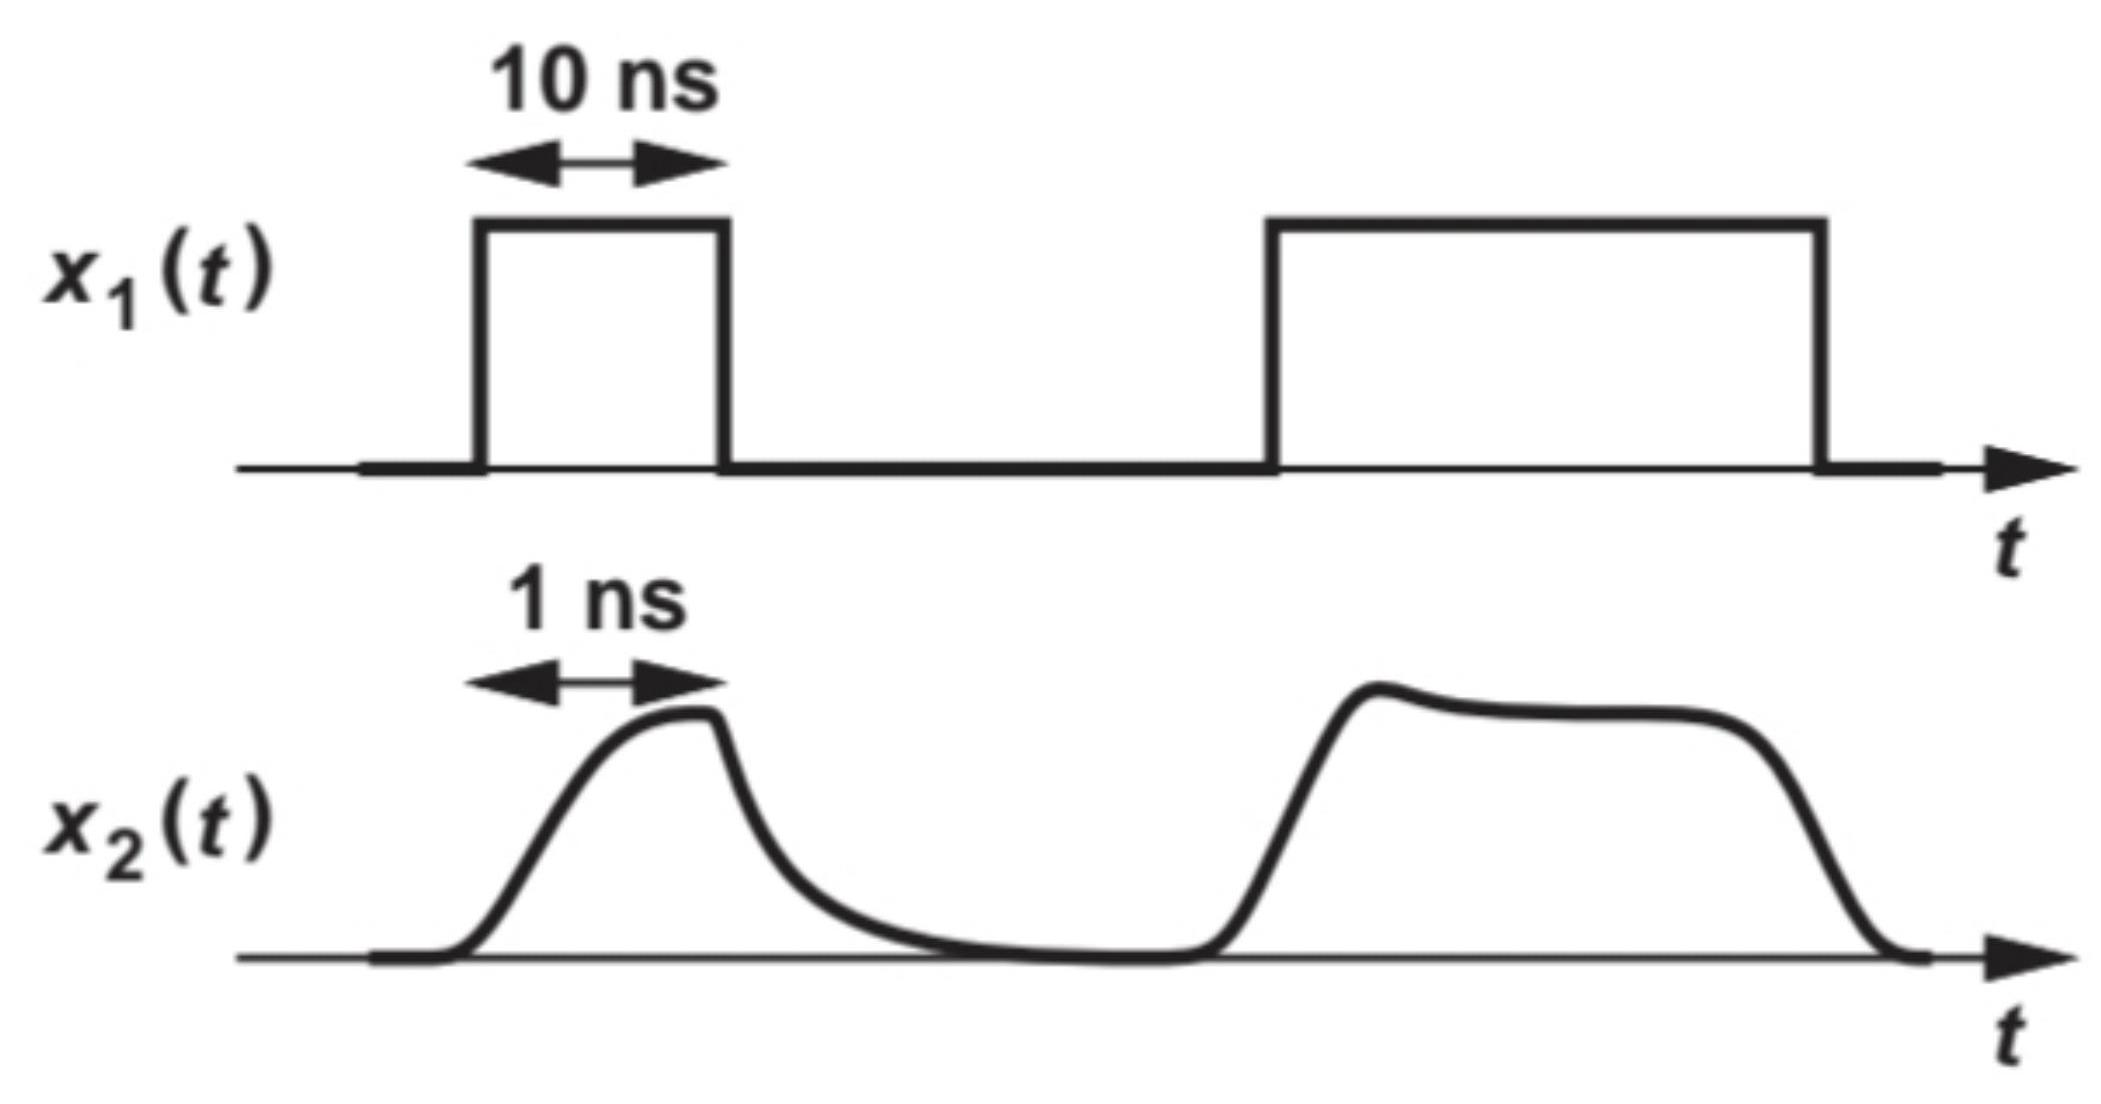
\includegraphics[max width=\textwidth, center]{2024_10_27_cec776a4495ed9df4dfcg-008}

Figure 1.8 Data waveforms at $100 \mathrm{Mb} / \mathrm{s}$ and $1 \mathrm{~Gb} / \mathrm{s}$.

\subsection*{1.3 BASIC CONCEPTS*}
Analysis of microelectronic circuits draws upon many concepts that are taught in basic courses on signals and systems and circuit theory. This section provides a brief review of these concepts so as to refresh the reader's memory and establish the terminology used throughout this book. The reader may first glance through this section to determine which topics need a review or simply return to this material as it becomes necessary later.

\subsection*{1.3.1 Analog and Digital Signals}
An electric signal is a waveform that carries information. Signals that occur in nature can assume all values in a given range. Called "analog," such signals include voice, video, seismic, and music waveforms. Shown in Fig. 1.9(a), an analog voltage\\
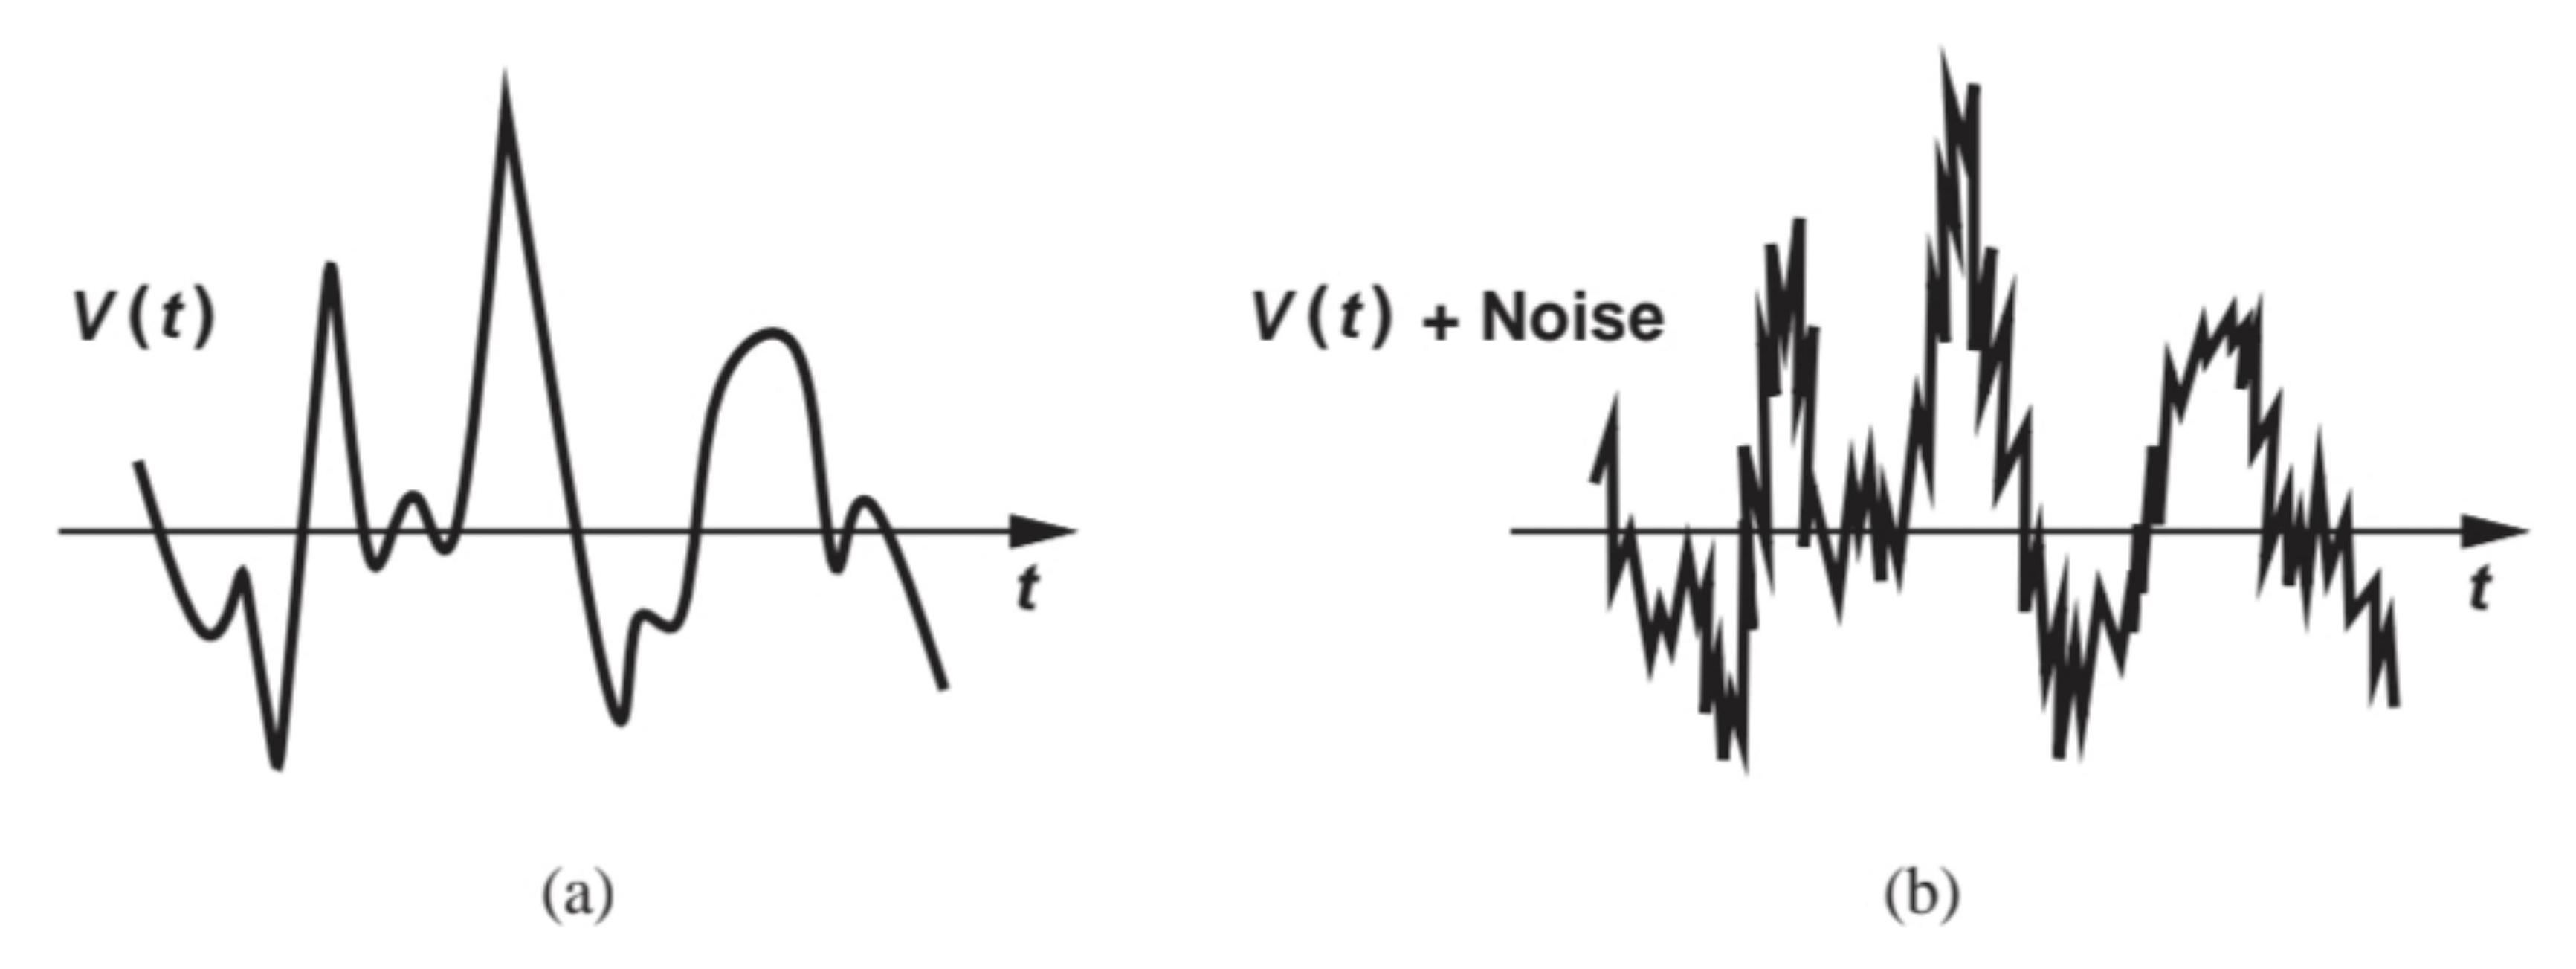
\includegraphics[max width=\textwidth, center]{2024_10_27_cec776a4495ed9df4dfcg-008(1)}

Figure 1.9 (a) Analog signal, (b) effect of noise on analog signal.

\footnotetext{*This section serves as a review and can be skipped in classroom teaching.
}
waveform swings through a "continuum" of values and provides information at each instant of time.

While occurring all around us, analog signals are difficult to "process" due to sensitivities to such circuit imperfections as "noise" and "distortion." As an example, Figure 1.9(b) illustrates the effect of noise. Furthermore, analog signals are difficult to "store" because they require "analog memories" (e.g., capacitors).

By contrast, a digital signal assumes only a finite number of values at only certain points in time. Depicted in Fig. 1.10(a) is a "binary" waveform, which remains at only one of two levels for each period, $T$. So long as the two voltages corresponding to ONEs and ZEROs differ sufficiently, logical circuits sensing such a signal process it correctly-even if noise or distortion create some corruption [Fig. 1.10(b)]. We therefore consider digital signals more "robust" than their analog counterparts. The storage of binary signals (in a digital memory) is also much simpler.\\
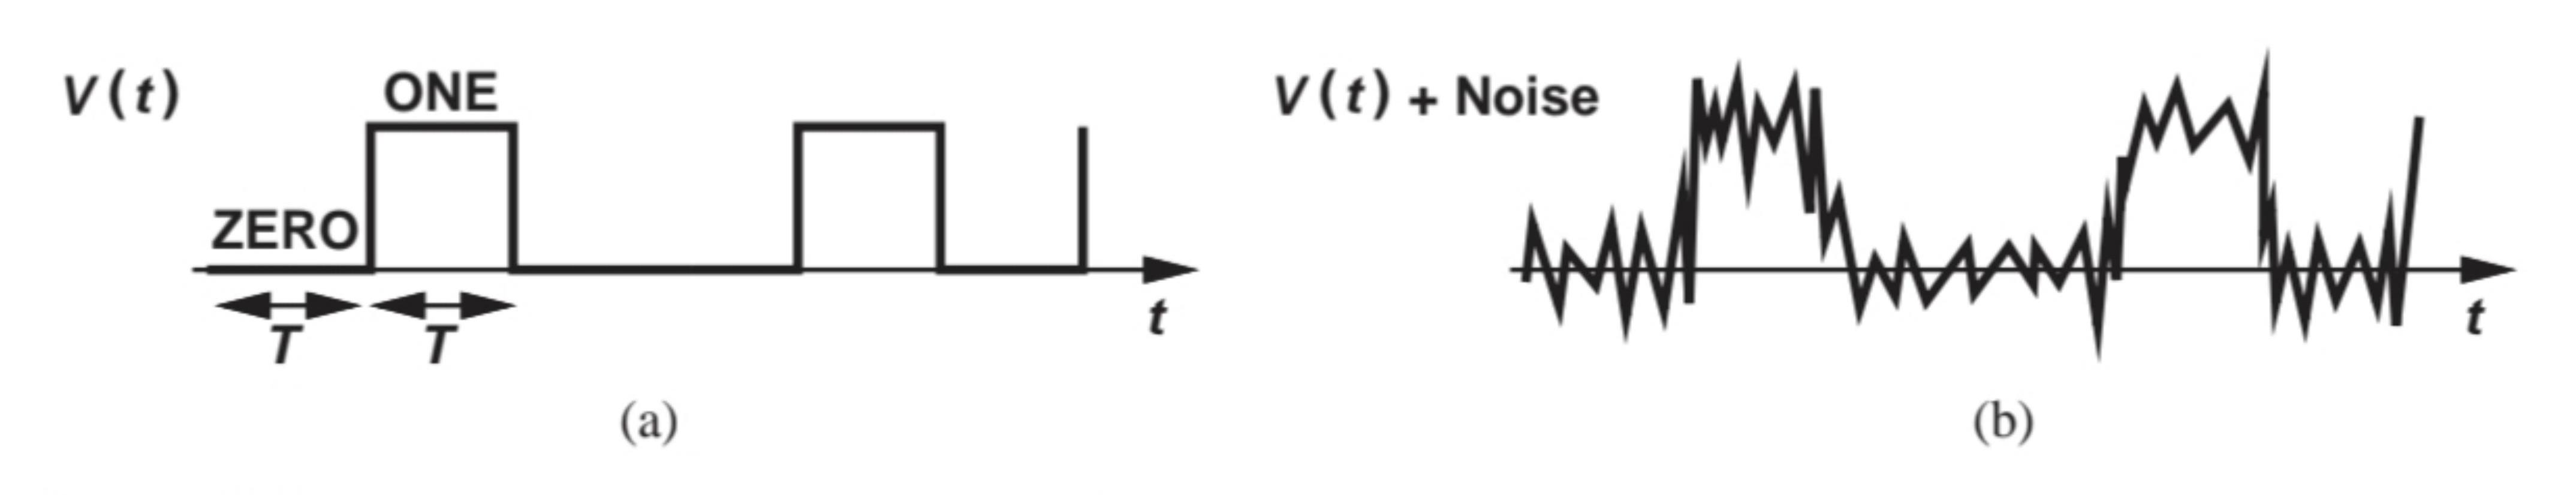
\includegraphics[max width=\textwidth, center]{2024_10_27_cec776a4495ed9df4dfcg-009(1)}

Figure 1.10 (a) Digital signal, (b) effect of noise on digital signal.

The foregoing observations favor processing of signals in the digital domain, suggesting that inherently analog information must be converted to digital form as early as possible. Indeed, complex microelectronic systems such as digital cameras, camcorders, and compact disk (CD) recorders perform some analog processing, "analog-to-digital conversion," and digital processing (Fig. 1.11), with the first two functions playing a critical role in the quality of the signal.\\
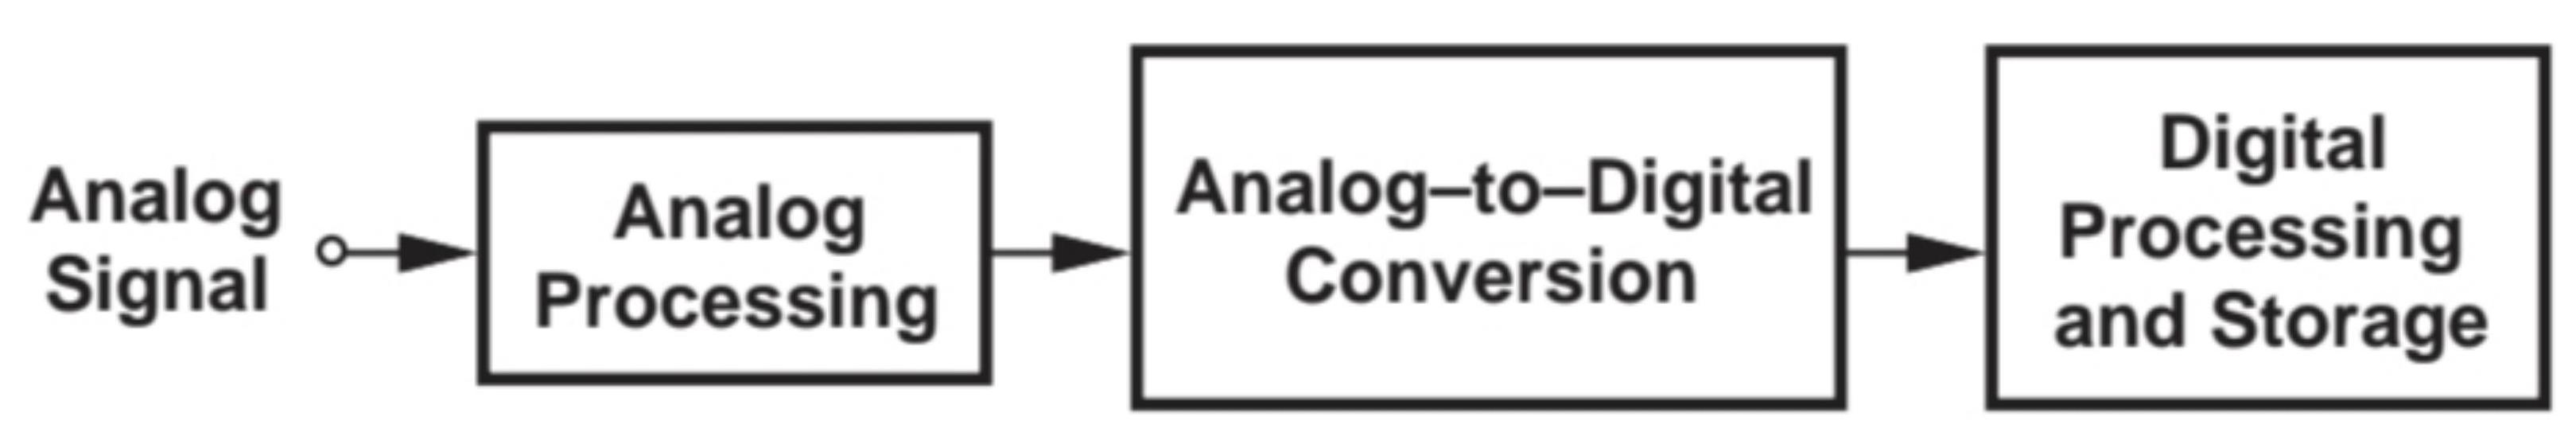
\includegraphics[max width=\textwidth, center]{2024_10_27_cec776a4495ed9df4dfcg-009}

Figure 1.11 Signal processing in a typical system.

It is worth noting that many digital binary signals must be viewed and processed as analog waveforms. Consider, for example, the information stored on a hard disk in a computer. Upon retrieval, the "digital" data appears as a distorted waveform with only a few millivolts of amplitude (Fig. 1.12). Such a small separation between ONEs and ZEROs proves inadequate if this signal is to drive a logical gate, demanding a great deal of amplification and other analog processing before the data reaches a robust digital form.

\footnotetext{${ }^{5}$ Distortion arises if the output is not a linear function of input.
}
\includegraphics[max width=\textwidth, center]{2024_10_27_cec776a4495ed9df4dfcg-010(1)}\\
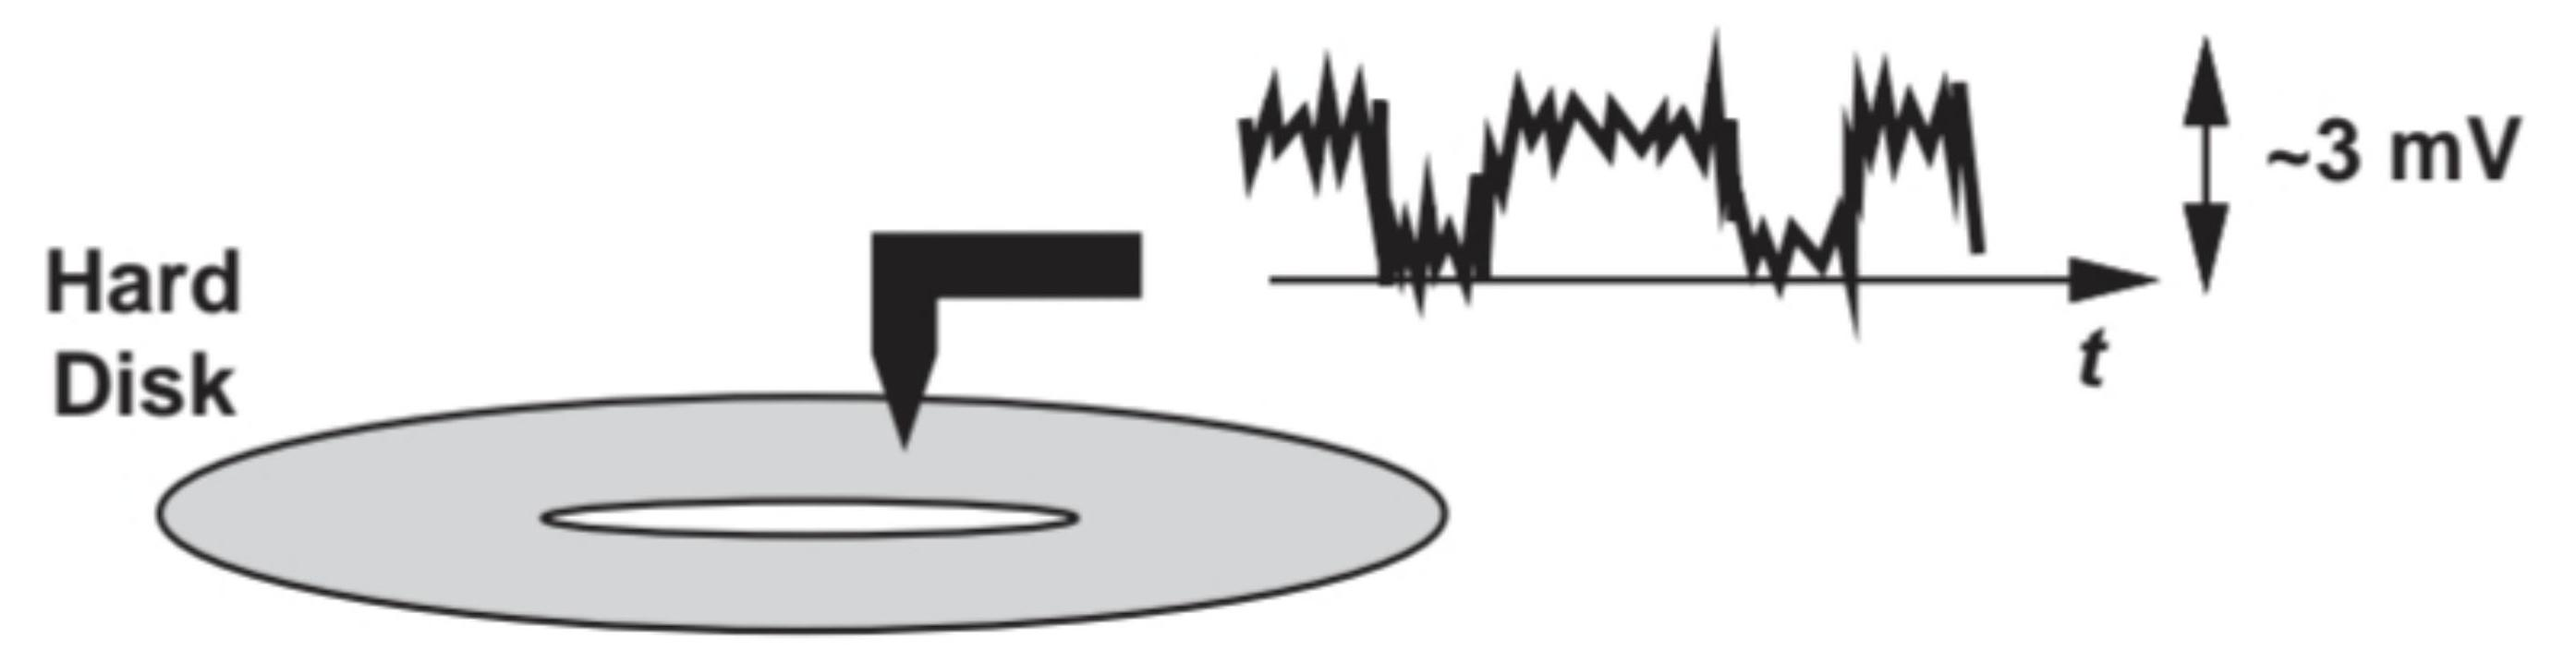
\includegraphics[max width=\textwidth, center]{2024_10_27_cec776a4495ed9df4dfcg-010}

Figure 1.12 Signal picked up from a hard disk in a computer.

\subsection*{1.3.2 Analog Circuits}
Today's microelectronic systems incorporate many analog functions. As exemplified by the cellphone and the digital camera studied above, analog circuits often limit the performance of the overall system.

The most commonly-used analog function is amplification. The signal received by a cellphone or picked up by a microphone proves too small to be processed further. An amplifier is therefore necessary to raise the signal swing to acceptable levels.

The performance of an amplifier is characterized by a number of parameters, e.g., gain, speed, and power dissipation. We study these aspects of amplification in great detail later in this book, but it is instructive to briefly review some of these concepts here.

A voltage amplifier produces an output swing greater than the input swing. The voltage gain, $A_{v}$, is defined as


\begin{equation*}
A_{v}=\frac{v_{\text {out }}}{v_{\text {in }}} \tag{1.1}
\end{equation*}


In some cases, we prefer to express the gain in decibels $(\mathrm{dB})$ :


\begin{equation*}
\left.A_{v}\right|_{\text {dB }}=20 \log \frac{v_{\text {out }}}{v_{\text {in }}} \tag{1.2}
\end{equation*}


For example, a voltage gain of 10 translates to 20 dB . The gain of typical amplifiers falls in the range of $10^{1}$ to $10^{5}$.

\begin{center}
\begin{tabular}{|c|c|c|}
\hline
\begin{tabular}{l}
Example \\
1.3 \\
\end{tabular} & \multicolumn{2}{|l|}{A cellphone receives a signal level of $20 \mu \mathrm{~V}$, but it must deliver a swing of 50 mV to the speaker that reproduces the voice. Calculate the required voltage gain in decibels.} \\
\hline
\multirow[t]{3}{*}{Solution} & We have &  \\
\hline
 & \( A_{v}=20 \log \frac{50 \mathrm{mV}}{20 \mu \mathrm{~V}} \) & (1.3) \\
\hline
 & $\approx 68 \mathrm{~dB}$. & (1.4) \\
\hline
\end{tabular}
\end{center}

Exercise What is the output swing if the gain is 50 dB ?

In order to operate properly and provide gain, an amplifier must draw power from a voltage source, e.g., a battery or a charger. Called the "power supply," this source is typically denoted by $V_{C C}$ or $V_{D D}$ [Fig. 1.13(a)]. In complex circuits, we may simplify the notation to that shown in Fig. 1.13(b), where the "ground" terminal signifies a reference point with zero potential. If the amplifier is simply denoted by a triangle, we may even omit the supply terminals [Fig. 1.13(c)], with the understanding that they are present. Typical amplifiers operate with supply voltages in the range of 1 V to 10 V .\\
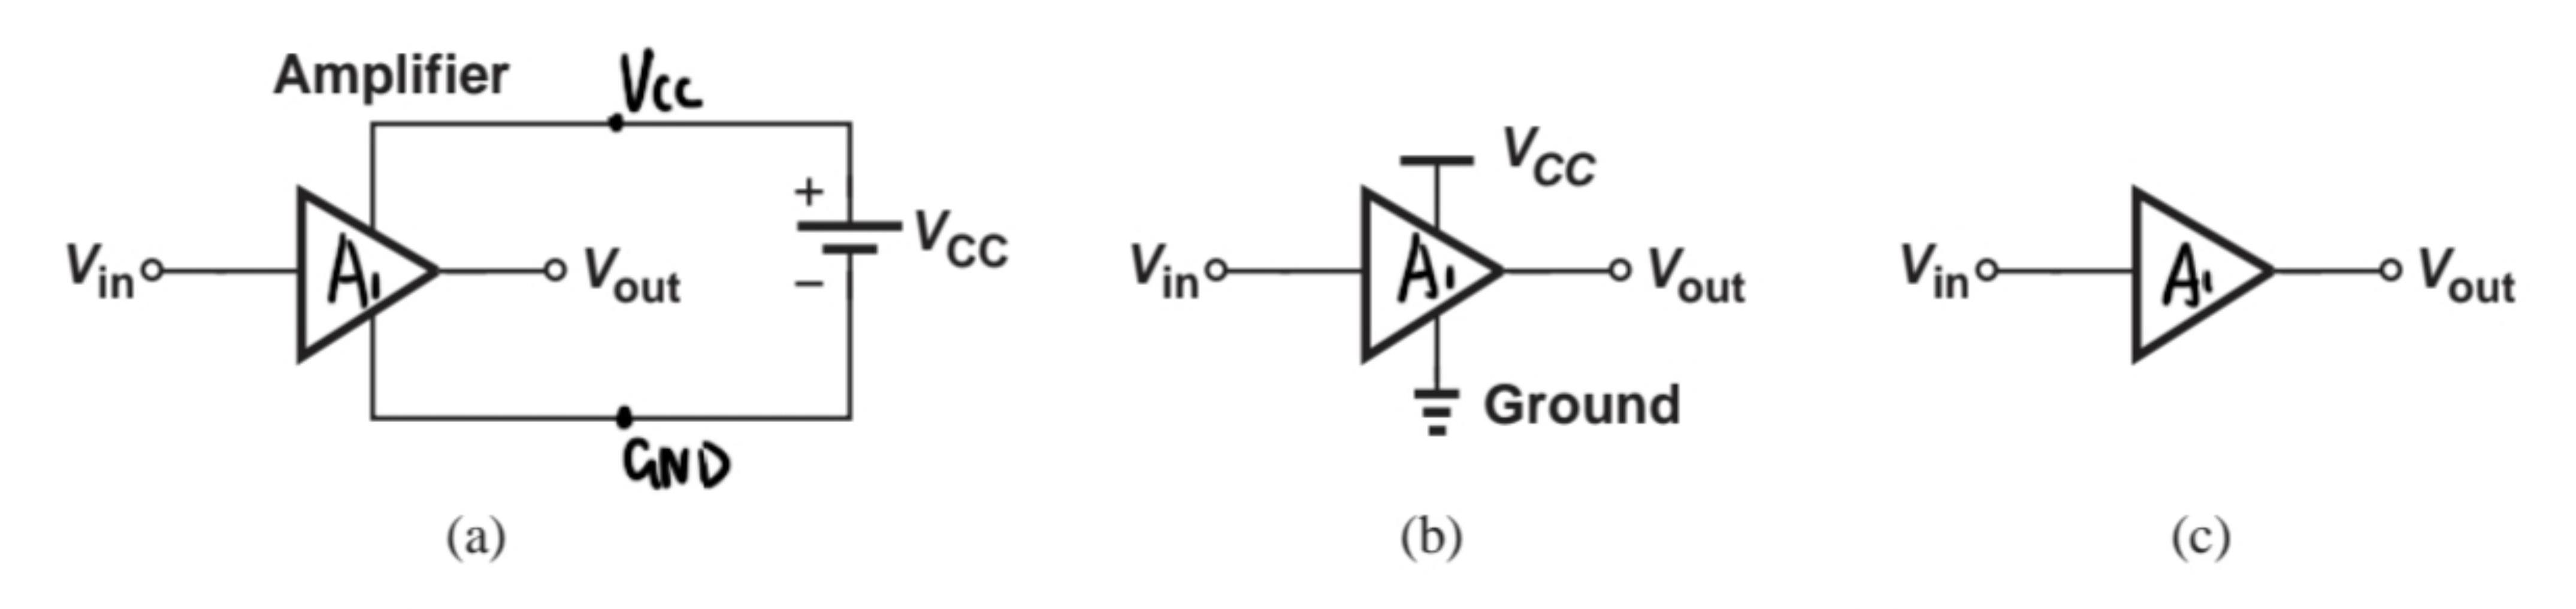
\includegraphics[max width=\textwidth, center]{2024_10_27_cec776a4495ed9df4dfcg-011(2)}

Figure 1.13 (a) General amplifier symbol along with its power supply, (b) simplified diagram of (a), (b) amplifier with supply rails omitted.

What limits the speed of amplifiers? We expect that various capacitances in the circuit begin to manifest themselves at high frequencies, thereby lowering the gain. In other words, as depicted in Fig. 1.14, the gain rolls off at sufficiently high frequencies, limiting the (usable) "bandwidth" of the circuit. Amplifiers (and other analog circuits) suffer from trade-offs between gain, speed and power dissipation. Today's microelectronic amplifiers achieve bandwidths as large as tens of gigahertz.\\
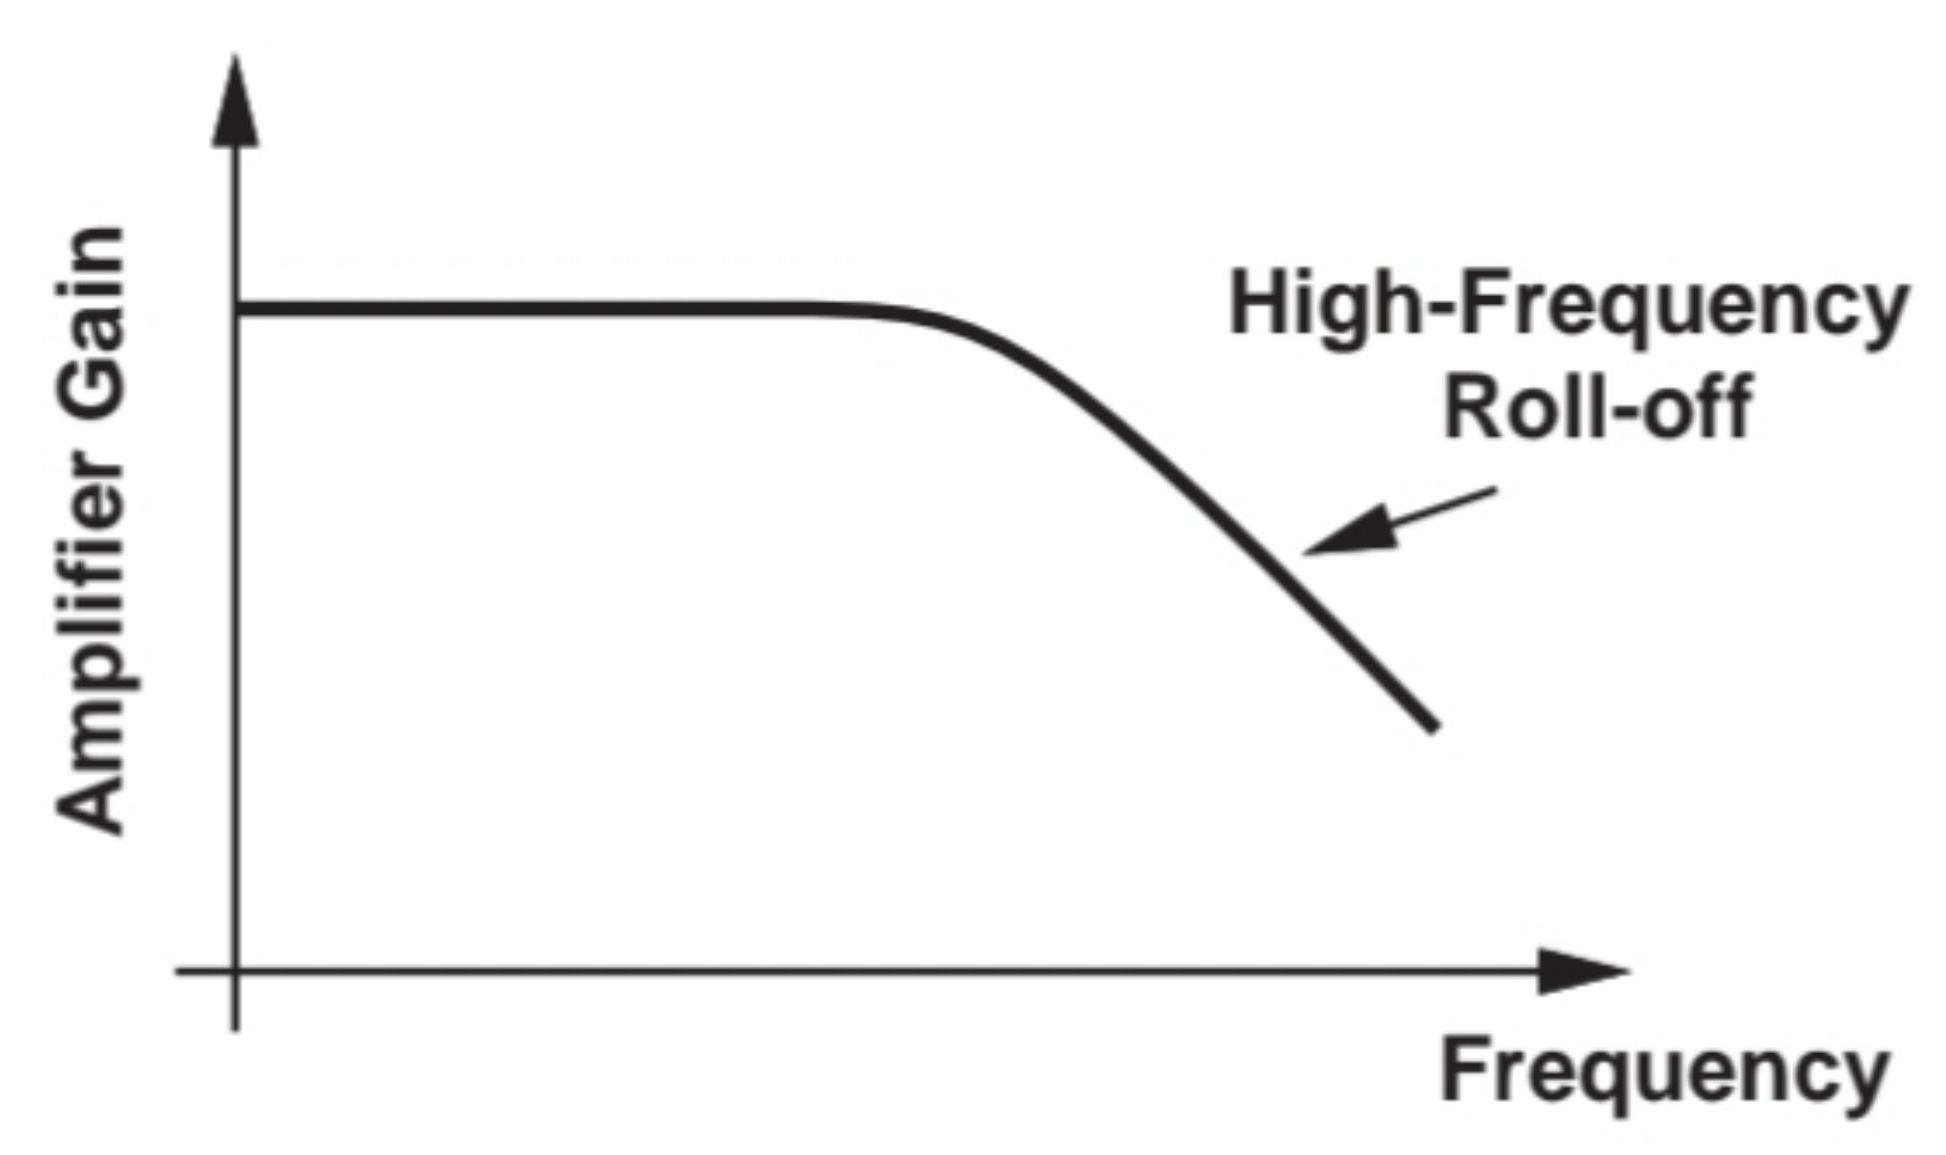
\includegraphics[max width=\textwidth, center]{2024_10_27_cec776a4495ed9df4dfcg-011(1)}

Figure 1.14 Roll-off of an amplifier's gain at high frequencies.\\
What other analog functions are frequently used? A critical operation is "filtering." For example, an electrocardiograph measuring a patient's heart activities also picks up the $60-\mathrm{Hz}$ ( or $50-\mathrm{Hz}$ ) electrical line voltage because the patient's body acts as an antenna. Thus, a filter must suppress this "interferer" to allow meaningful measurement of the heart.

\subsection*{1.3.3 Digital Circuits}
More than $80 \%$ of the microelectronics industry deals with digital circuits. Examples include microprocessors, static and dynamic memories, and digital signal processors. Recall from basic logic design that gates form "combinational" circuits, and latches and flipflops constitute "sequential" machines. The complexity, speed, and power dissipation of these building blocks play a central role in the overall system performance.

In digital microelectronics, we study the design of the internal circuits of gates, flipflops, and other components. For example, we construct a circuit using devices such as transistors to realize the NOT and NOR functions shown in Fig. 1.15. Based on these implementations, we then determine various properties of each circuit. For example, what limits the speed\\
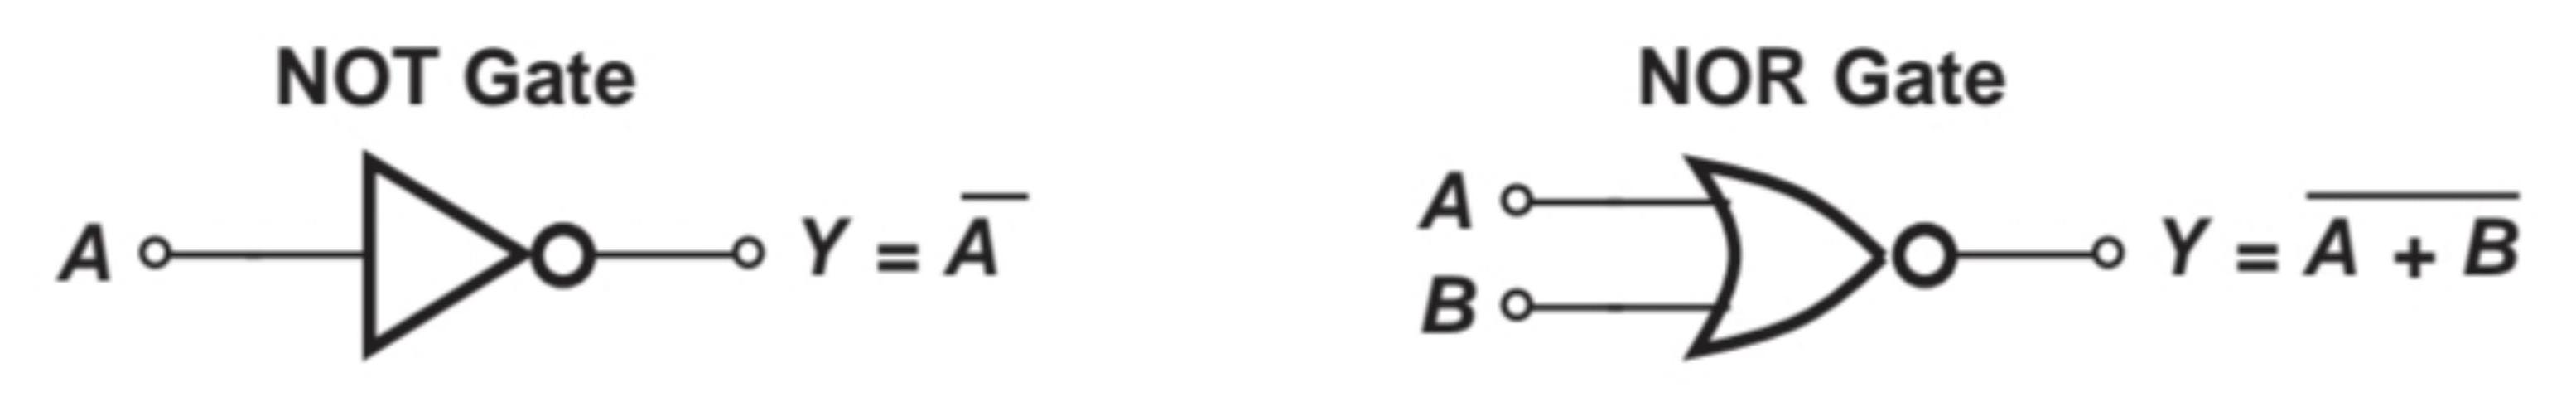
\includegraphics[max width=\textwidth, center]{2024_10_27_cec776a4495ed9df4dfcg-011}

Figure 1.15 NOT and NOR gates.\\
\includegraphics[max width=\textwidth, center]{2024_10_27_cec776a4495ed9df4dfcg-012}

12 Chapter 1 Introduction to Microelectronics\\
of a gate? How much power does a gate consume while running at a certain speed? How robustly does a gate operate in the presence of nonidealities such as noise (Fig. 1.16)?\\
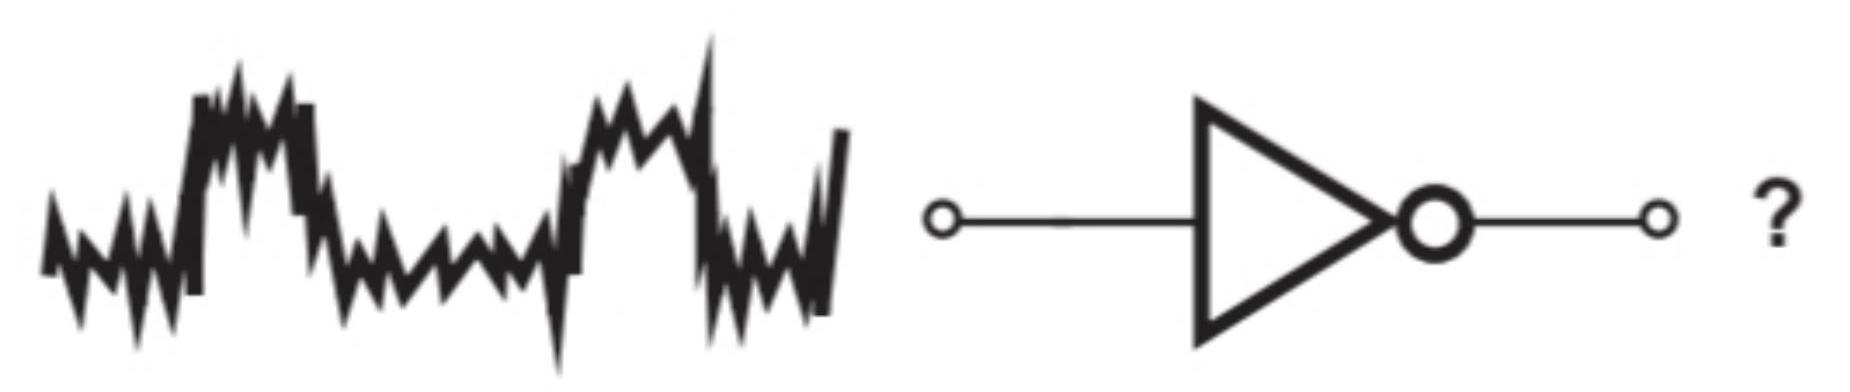
\includegraphics[max width=\textwidth, center]{2024_10_27_cec776a4495ed9df4dfcg-012(1)}

Figure 1.16 Response of a gate to a noisy input.

Example Consider the circuit shown in Fig. 1.17, where switch $S_{1}$ is controlled by the digital input.\\
That is, if $A$ is high, $S_{1}$ is on and vice versa. Prove that the circuit provides the NOT function.

Figure 1.17\\
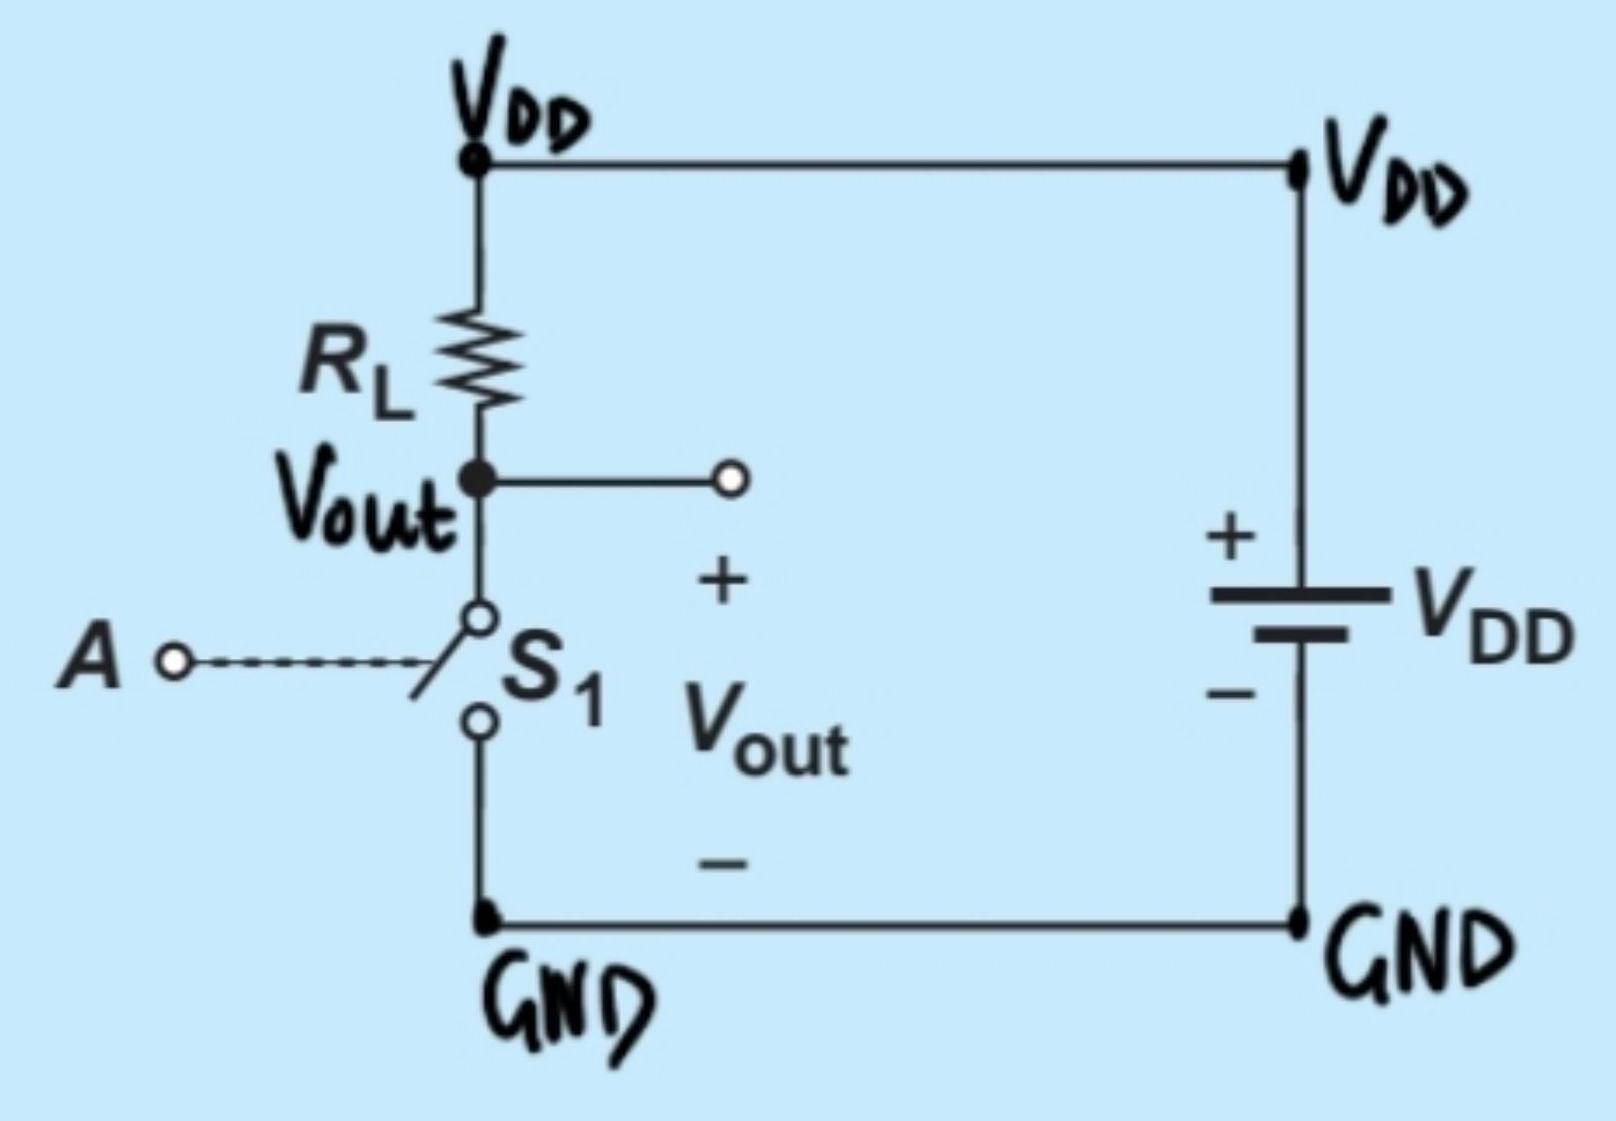
\includegraphics[max width=\textwidth, center]{2024_10_27_cec776a4495ed9df4dfcg-012(2)}

Solution If $A$ is high, $S_{1}$ is on, forcing $V_{\text {out }}$ to zero. On the other hand, if $A$ is low, $S_{1}$ remains off, drawing no current from $R_{L}$. As a result, the voltage drop across $R_{L}$ is zero and hence $V_{\text {out }}=V_{D D}$; i.e., the output is high. We thus observe that, for both logical states at the input, the output assumes the opposite state.

Exercise Determine the logical function if $S_{1}$ and $R_{L}$ are swapped and $V_{\text {out }}$ is sensed across $R_{L}$.

The above example indicates that switches can perform logical operations. In fact, early digital circuits did employ mechanical switches (relays), but suffered from a very limited speed (a few kilohertz). It was only after "transistors" were invented and their ability to act as switches was recognized that digital circuits consisting of millions of gates and operating at high speeds (several gigahertz) became possible.

\subsection*{1.3.4 Basic Circuit Theorems}
Of the numerous analysis techniques taught in circuit theory courses, some prove particularly important to our study of microelectronics. This section provides a review of such concepts.

Kirchoff's Laws The Kirchoff Current Law (KCL) states that the sum of all currents flowing into a node is zero (Fig. 1.18):


\begin{equation*}
\sum_{j} I_{j}=0 \tag{1.5}
\end{equation*}


KCL in fact results from conservation of charge: a nonzero sum would mean that either some of the charge flowing into node $X$ vanishes or this node produces charge.\\
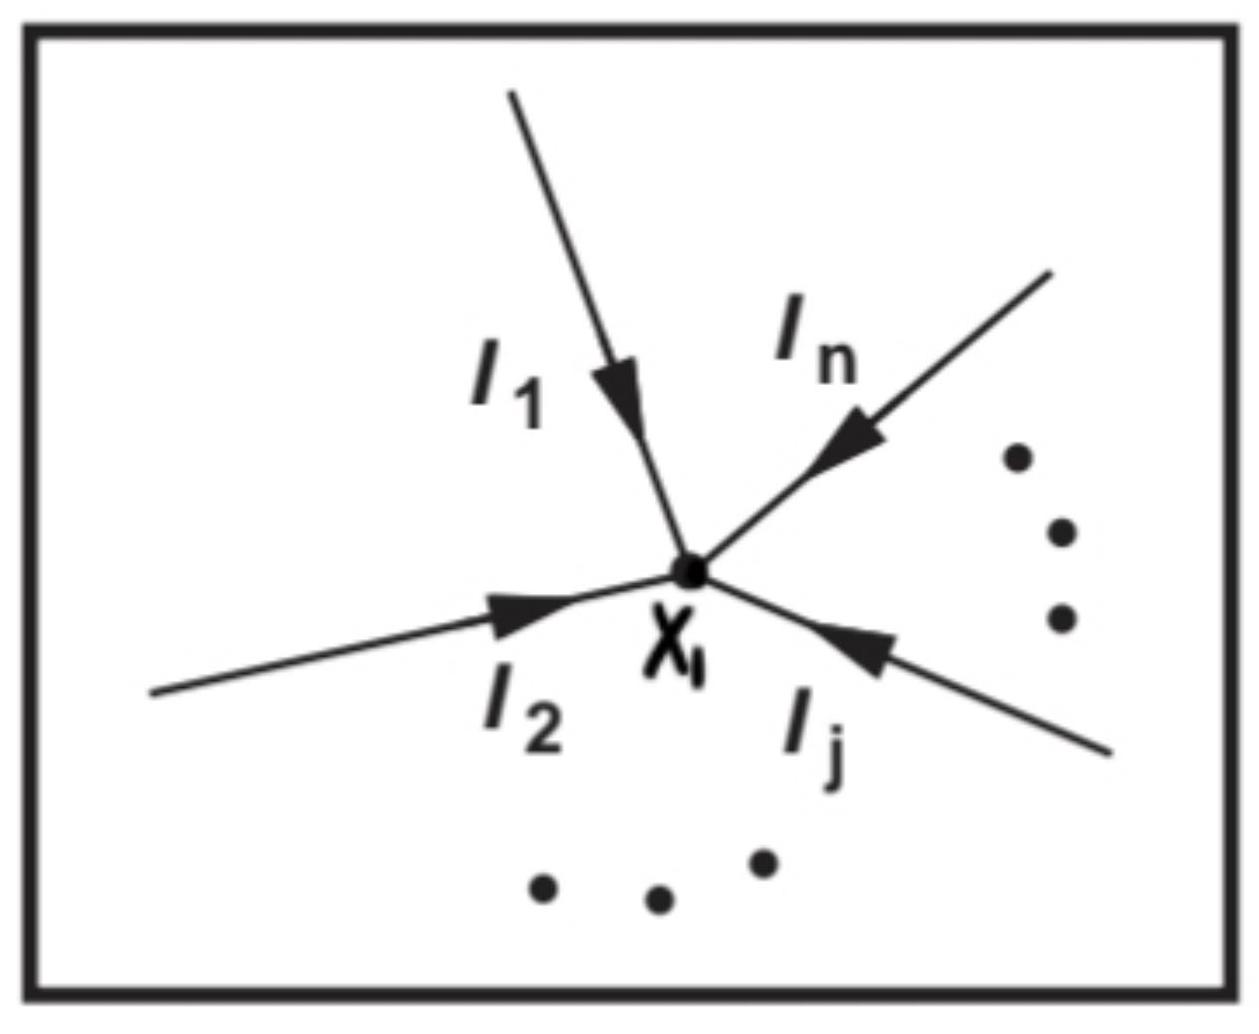
\includegraphics[max width=\textwidth, center]{2024_10_27_cec776a4495ed9df4dfcg-013}

Figure 1.18 Illustration of KCL.\\
The Kirchoff Voltage Law (KVL) states that the sum of voltage drops around any closed loop in a circuit is zero [Fig. 1.19(a)]:\\
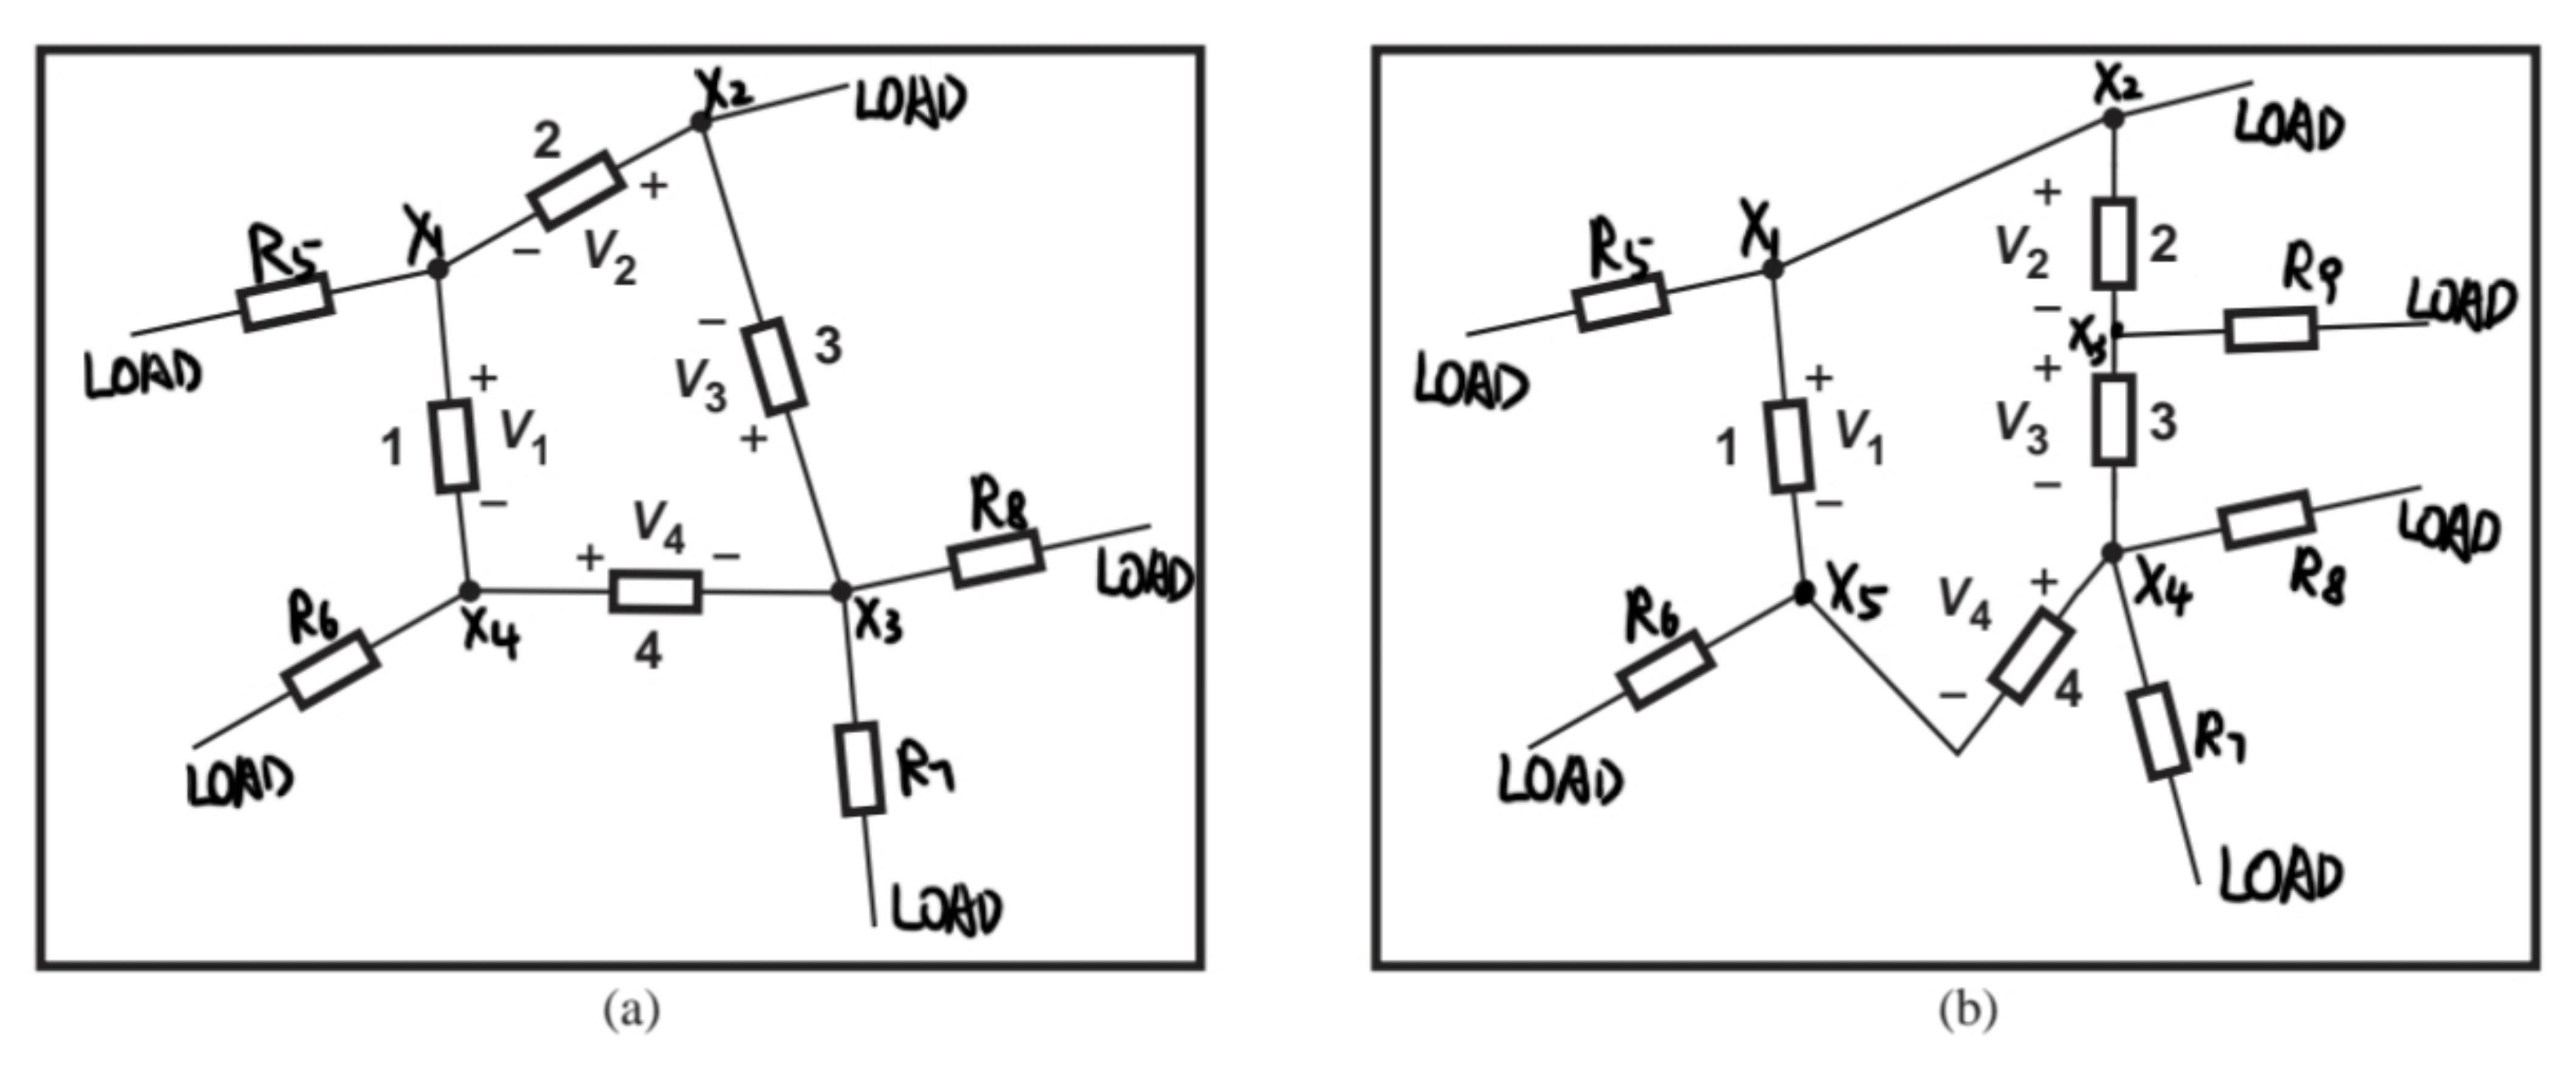
\includegraphics[max width=\textwidth, center]{2024_10_27_cec776a4495ed9df4dfcg-013(1)}

Figure 1.19 (a) Illustration of KVL, (b) slightly different view of the circuit.


\begin{equation*}
\sum_{j} V_{j}=0, \tag{1.6}
\end{equation*}


where $V_{j}$ denotes the voltage drop across element number $j$. KVL arises from the conservation of the "electromotive force." In the example illustrated in Fig. 1.19(a), we may sum the voltages in the loop to zero: $V_{1}+V_{2}+V_{3}+V_{4}=0$. Alternatively, adopting the modified view shown in Fig. 1.19(b), we can say $V_{1}$ is equal to the sum of the voltages across elements 2, 3, and 4: $V_{1}=V_{2}+V_{3}+V_{4}$. Note that the polarities assigned to $V_{2}$, $V_{3}$, and $V_{4}$ in Fig. 1.19(b) are different from those in Fig. 1.19(a).

In solving circuits, we may not know a priori the correct polarities of the currents and voltages. Nonetheless, we can simply assign arbitrary polarities, write KCLs and KVLs, and solve the equations to obtain the actual polarities and values.

The topology depicted in Fig. 1.20 represents the equivalent circuit of an amplifier. The dependent current source $i_{1}$ is equal to a constant, $g_{m},{ }^{6}$ multiplied by the voltage drop across $r_{\pi}$. Determine the voltage gain of the amplifier, $v_{\text {out }} / v_{i n}$.

\footnotetext{${ }^{6}$ What is the dimension of $g_{m}$ ?
}\section*{\begin{center}
\includegraphics[max width=\textwidth]{2024_10_27_cec776a4495ed9df4dfcg-014(1)}
\end{center}}
14 Chapter 1 Introduction to Microelectronics

Figure 1.20\\
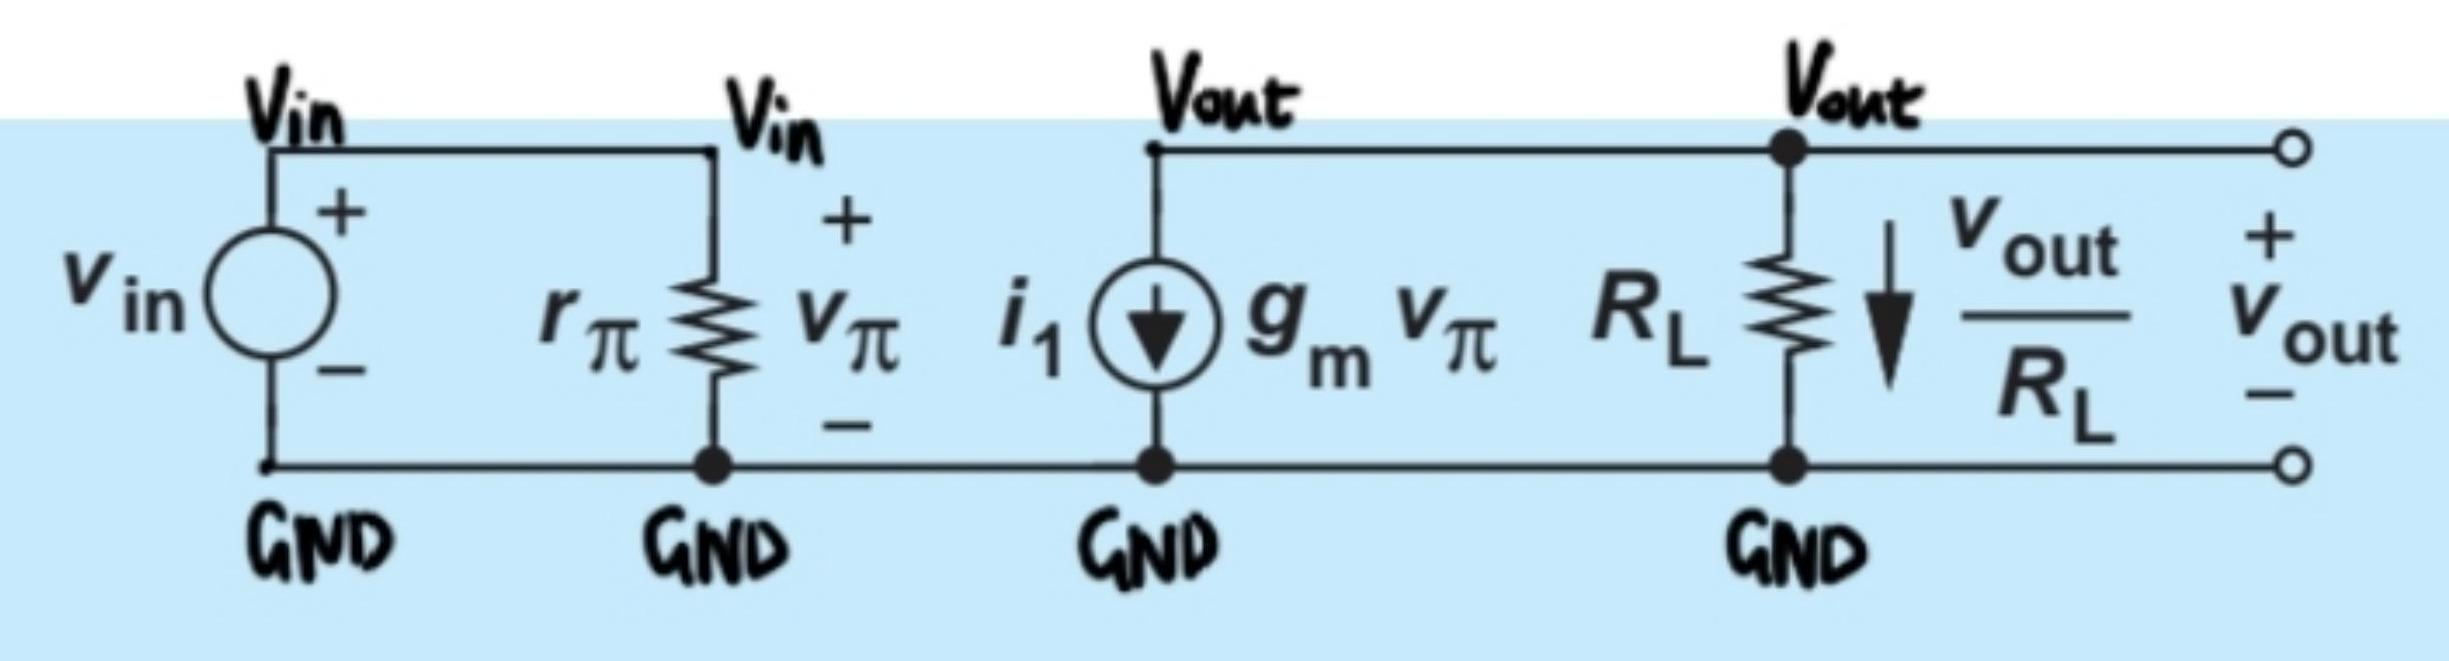
\includegraphics[max width=\textwidth, center]{2024_10_27_cec776a4495ed9df4dfcg-014}

Solution We must compute $V_{\text {out }}$ in terms of $v_{\text {in }}$, i.e., we must eliminate $v_{\pi}$ from the equations. Writing a KVL in the "input loop," we have


\begin{equation*}
v_{i n}=v_{\pi} \tag{1.7}
\end{equation*}


and hence $g_{m} v_{\pi}=g_{m} v_{i n}$. A KCL at the output node yields


\begin{equation*}
g_{m} v_{\pi}+\frac{v_{\text {out }}}{R_{L}}=0 \tag{1.8}
\end{equation*}


It follows that


\begin{equation*}
\frac{v_{\text {out }}}{v_{\text {in }}}=-g_{m} R_{L} \tag{1.9}
\end{equation*}


Note that the circuit amplifies the input if $g_{m} R_{L}>1$. Unimportant in most cases, the negative sign simply means the circuit "inverts" the signal.

Exercise Repeat the above example if $r_{\pi} \rightarrow \infty$.

Example\\
1.6

Figure 1.21 shows another amplifier topology. Compute the gain.\\
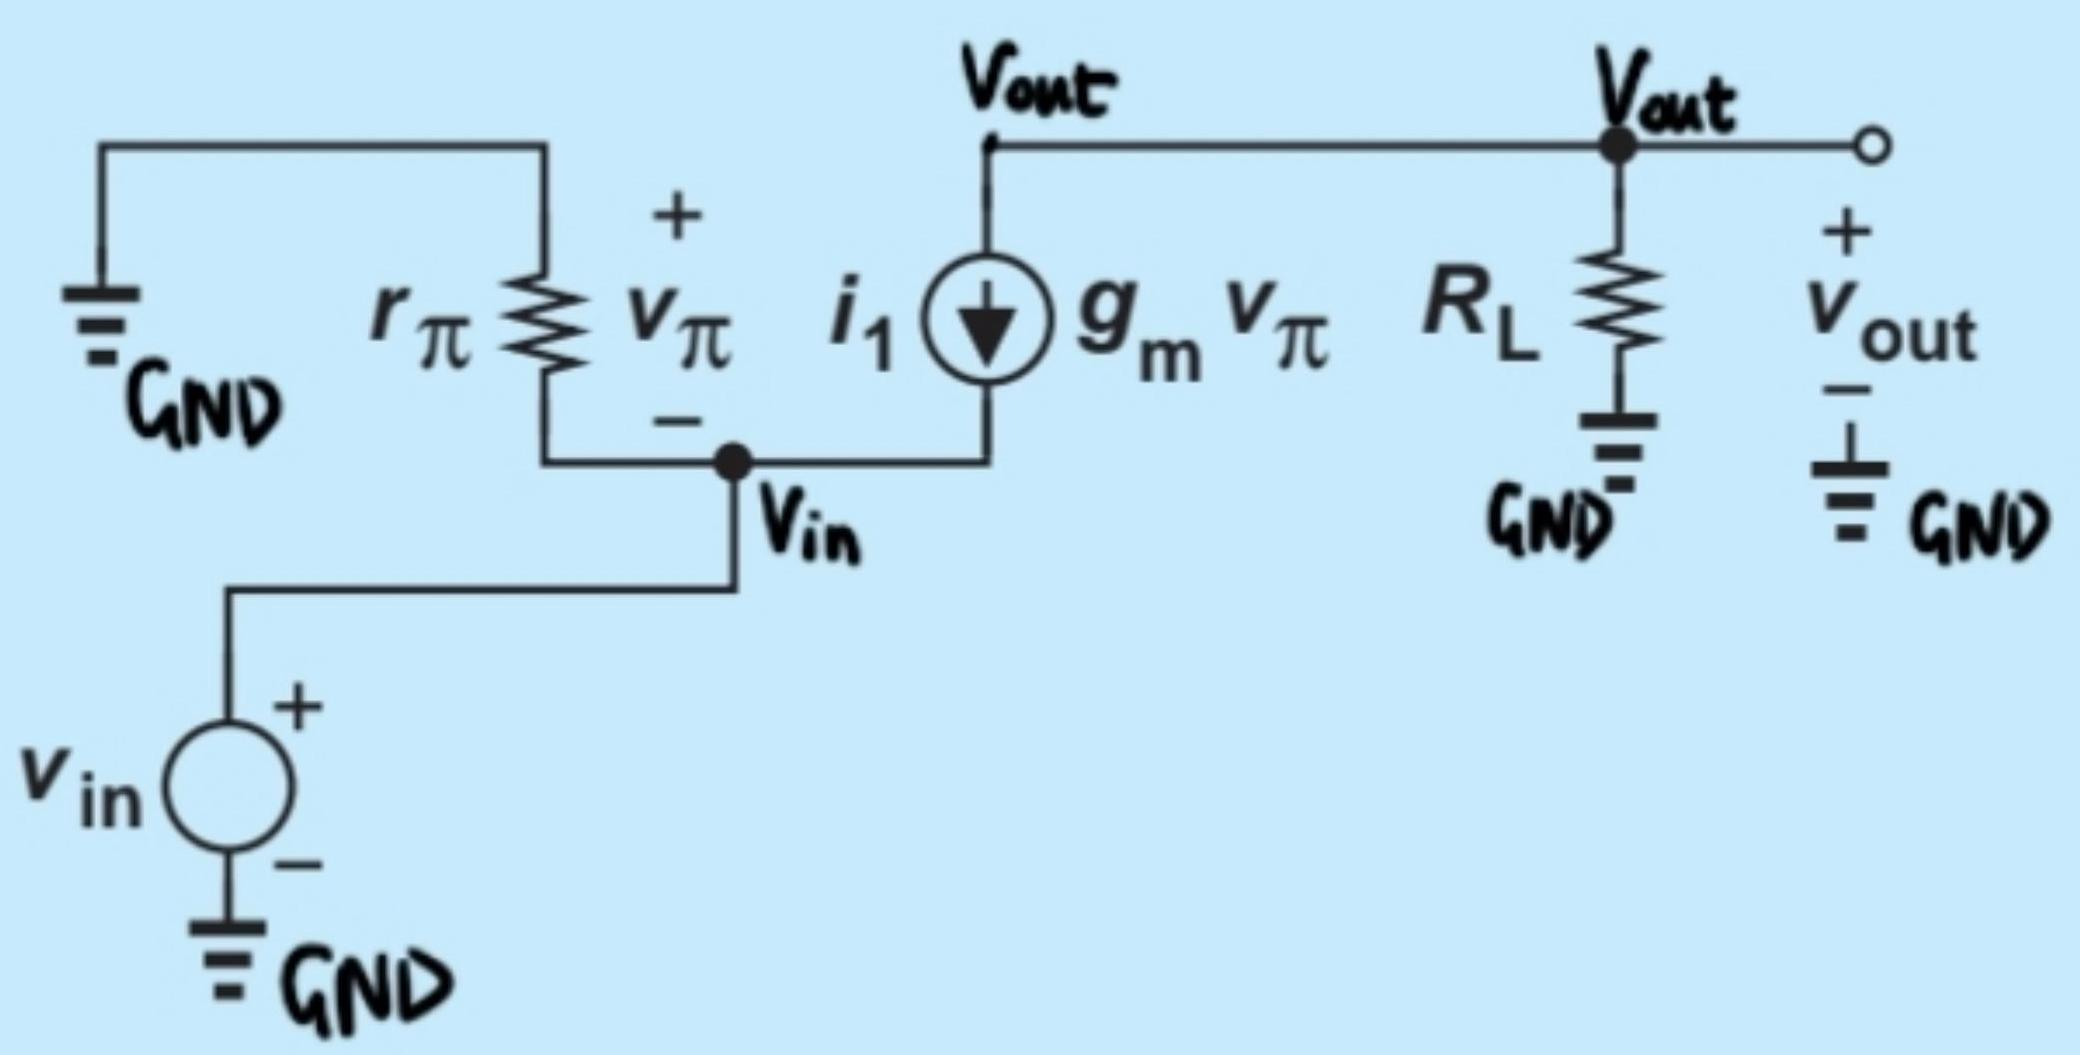
\includegraphics[max width=\textwidth, center]{2024_10_27_cec776a4495ed9df4dfcg-014(2)}

Figure 1.21\\
Solution Noting that $r_{\pi}$ in fact appears in parallel with $v_{i n}$, we write a KVL across these two components:


\begin{equation*}
v_{i n}=-v_{\pi} \tag{1.10}
\end{equation*}


The KCL at the output node is similar to (1.8). Thus,


\begin{equation*}
\frac{v_{\text {out }}}{v_{\text {in }}}=g_{m} R_{L} \tag{1.11}
\end{equation*}


Interestingly, this type of amplifier does not invert the signal.\\
Exercise $\quad$ Repeat the above example if $r_{\pi} \rightarrow \infty$.

Example\\
1.7

A third amplifier topology is shown in Fig. 1.22. Determine the voltage gain.\\
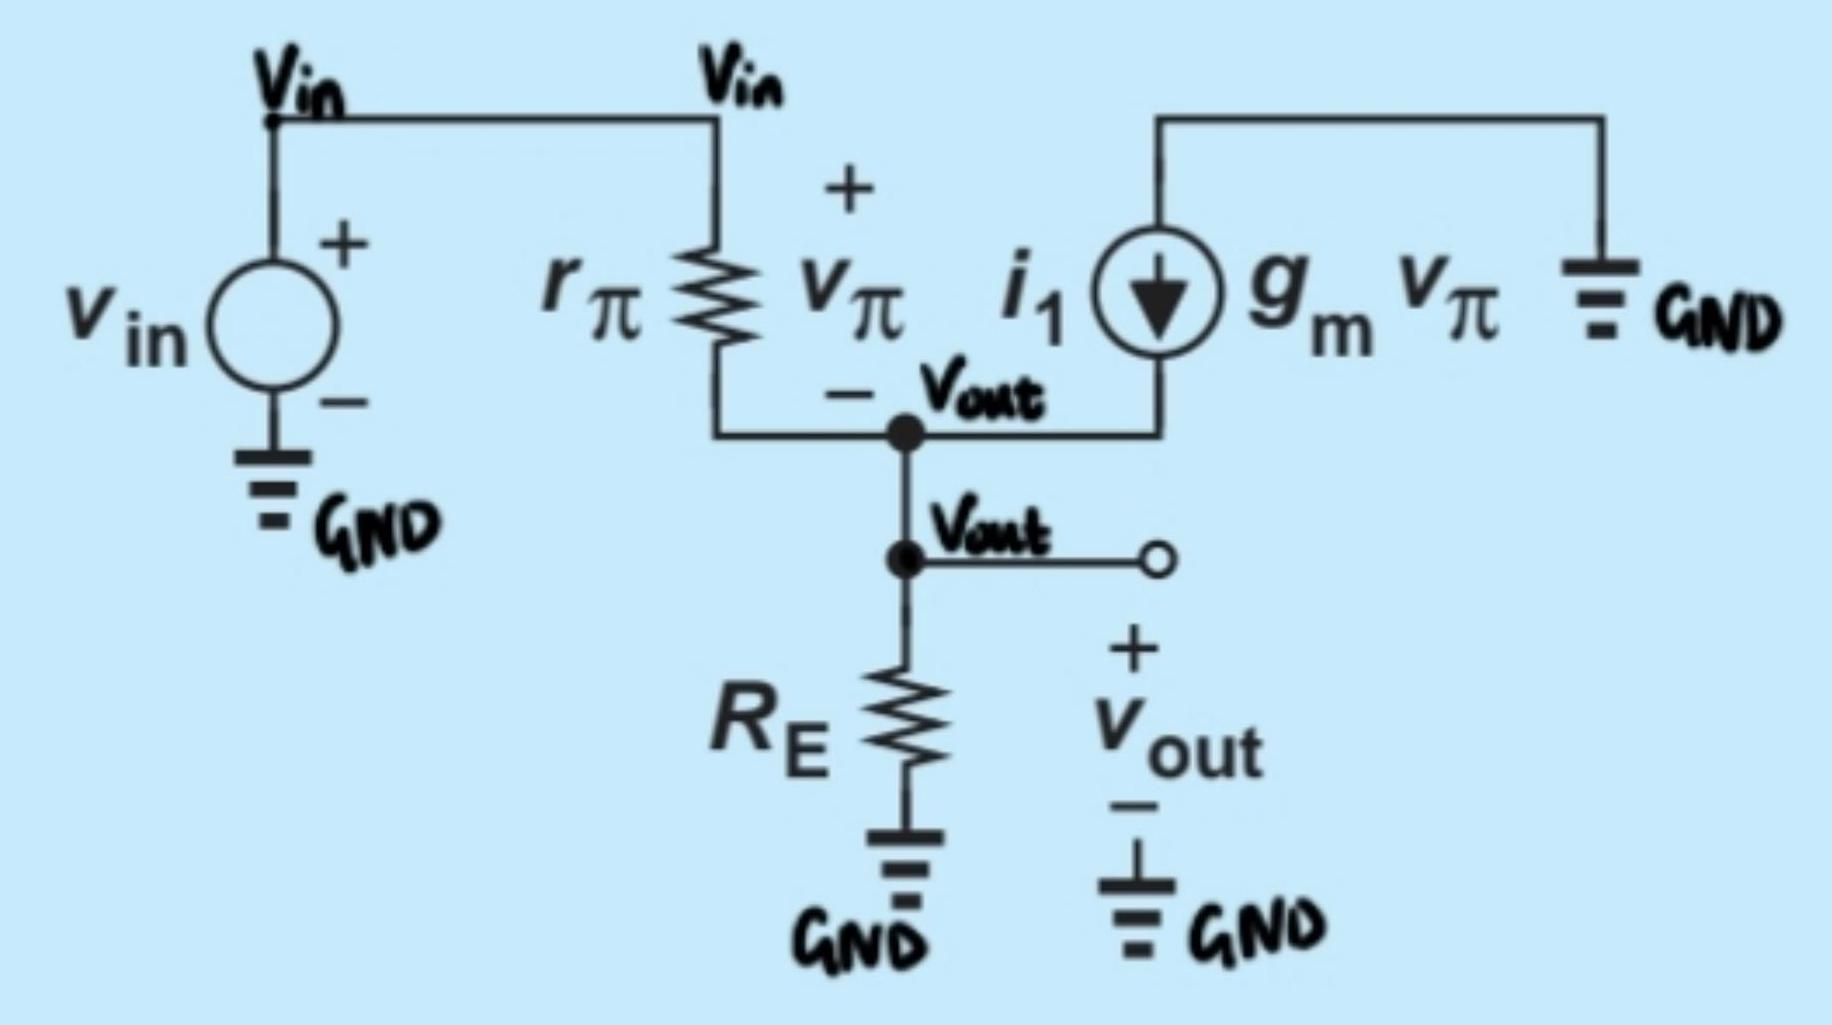
\includegraphics[max width=\textwidth, center]{2024_10_27_cec776a4495ed9df4dfcg-015}

Figure 1.22\\
Solution We first write a KVL around the loop consisting of $v_{i n}, r_{\pi}$, and $R_{E}$ :


\begin{equation*}
v_{\text {in }}=v_{\pi}+v_{\text {out }} \tag{1.12}
\end{equation*}


That is, $v_{\pi}=v_{\text {in }}-v_{\text {out }}$. Next, noting that the currents $v_{\pi} / r_{\pi}$ and $g_{m} v_{\pi}$ flow into the output node, and the current $v_{\text {out }} / R_{E}$ flows out of it, we write a KCL:


\begin{equation*}
\frac{v_{\pi}}{r_{\pi}}+g_{m} v_{\pi}=\frac{v_{\text {out }}}{R_{E}} \tag{1.13}
\end{equation*}


Substituting $v_{\text {in }}-v_{\text {out }}$ for $v_{\pi}$ gives


\begin{equation*}
v_{\text {in }}\left(\frac{1}{r_{\pi}}+g_{m}\right)=v_{\text {out }}\left(\frac{1}{R_{E}}+\frac{1}{r_{\pi}}+g_{m}\right) \tag{1.14}
\end{equation*}


and hence


\begin{align*}
\frac{v_{\text {out }}}{v_{\text {in }}} & =\frac{\frac{1}{r_{\pi}}+g_{m}}{\frac{1}{R_{E}}+\frac{1}{r_{\pi}}+g_{m}}  \tag{1.15}\\
& =\frac{\left(1+g_{m} r_{\pi}\right) R_{E}}{r_{\pi}+\left(1+g_{m} r_{\pi}\right) R_{E}} \tag{1.16}
\end{align*}


Note that the voltage gain always remains below unity. Would such an amplifier prove useful at all? In fact, this topology exhibits some important properties that make it a versatile building block.

Exercise Repeat the above example if $r_{\pi} \rightarrow \infty$.

The foregoing three examples relate to three amplifier topologies that are studied extensively in Chapter 5.

Thevenin and Norton Equivalents While Kirchoff's laws can always be utilized to solve any circuit, the Thevenin and Norton theorems can both simplify the algebra and, more importantly, provide additional insight into the operation of a circuit.

Thevenin's theorem states that a (linear) one-port network can be replaced with an equivalent circuit consisting of one voltage source in series with one impedance. Illustrated in Fig. 1.23(a), the term "port" refers to any two nodes whose voltage difference is of interest. The equivalent voltage, $v_{\mathrm{Thev}}$, is obtained by leaving the port open and computing the voltage created by the actual circuit at this port. The equivalent impedance, $Z_{\mathrm{Thev}}$, is\\
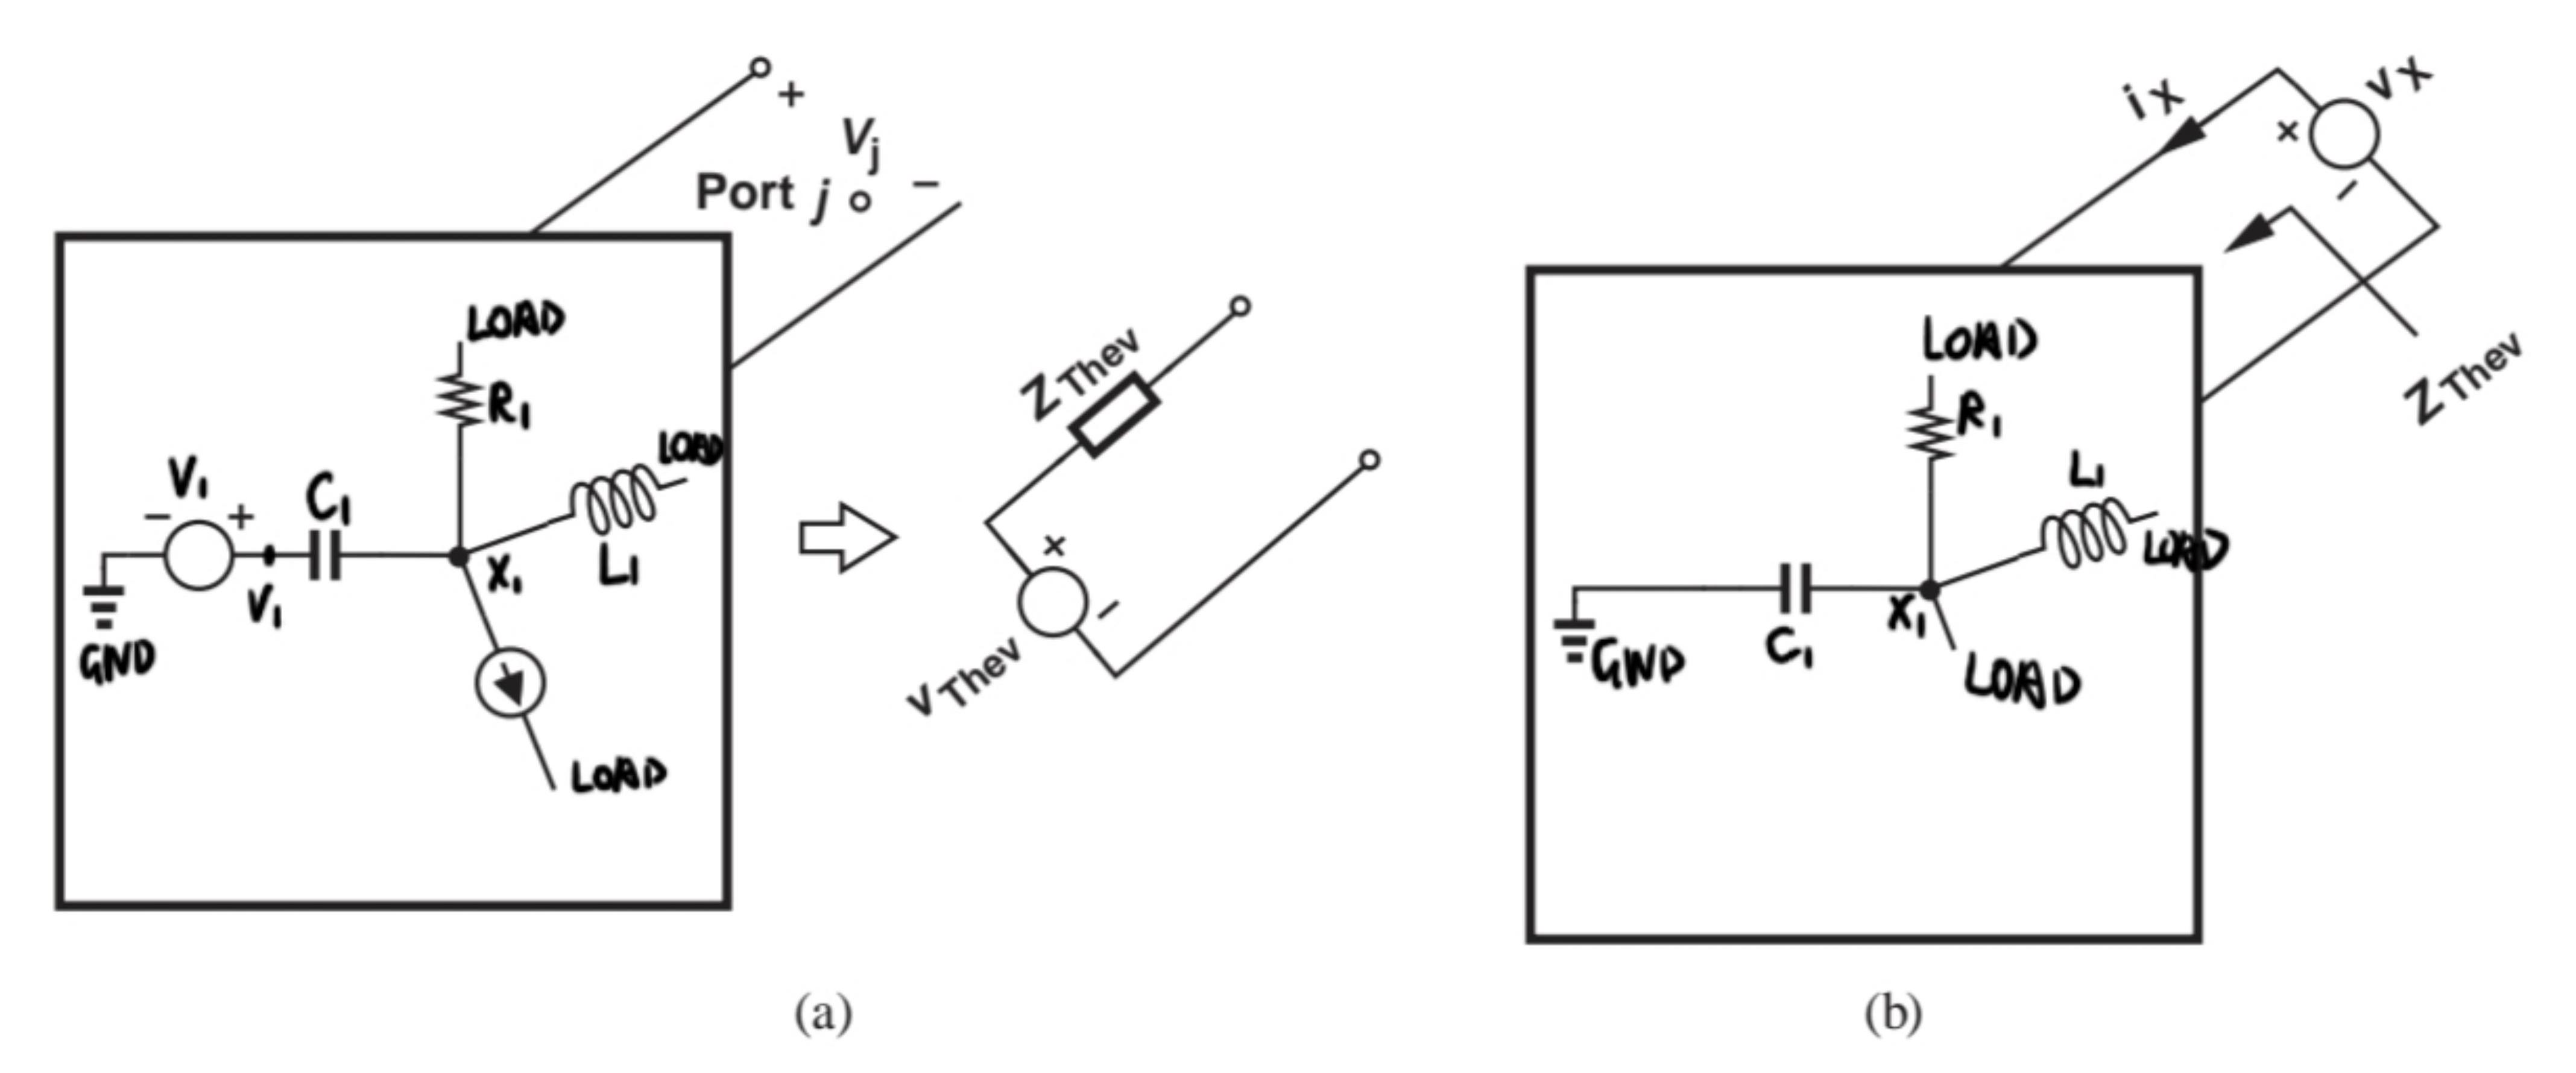
\includegraphics[max width=\textwidth, center]{2024_10_27_cec776a4495ed9df4dfcg-016(1)}

Figure 1.23 (a) Thevenin equivalent circuit, (b) computation of equivalent impedance.\\
determined by setting all independent voltage and current sources in the circuit to zero and calculating the impedance between the two nodes. We also call $Z_{\text {Thev }}$ the impedance "seen" when "looking" into the output port [Fig. 1.23(b)]. The impedance is computed by applying a voltage source across the port and obtaining the resulting current. A few examples illustrate these principles.

Example\\
1.8

Solution\\
We must compute the open-circuit output voltage and the impedance seen when looking into the output port. The Thevenin voltage is obtained from Fig. 1.24(a) and Eq. (1.9):


\begin{align*}
v_{\text {Thev }} & =v_{\text {out }}  \tag{1.17}\\
& =-g_{m} R_{L} v_{\text {in }} . \tag{1.18}
\end{align*}


To calculate $Z_{\text {Thev }}$, we set $v_{\text {in }}$ to zero, apply a voltage source, $v_{X}$, across the output port, and determine the current drawn from the voltage source, $i_{X}$. As shown in Fig. 1.24(b), setting $v_{i n}$ to zero means replacing it with a short circuit. Also, note that the current source $g_{m} v_{\pi}$ remains in the circuit because it depends on the voltage across $r_{\pi}$, whose value is not known a priori.\\
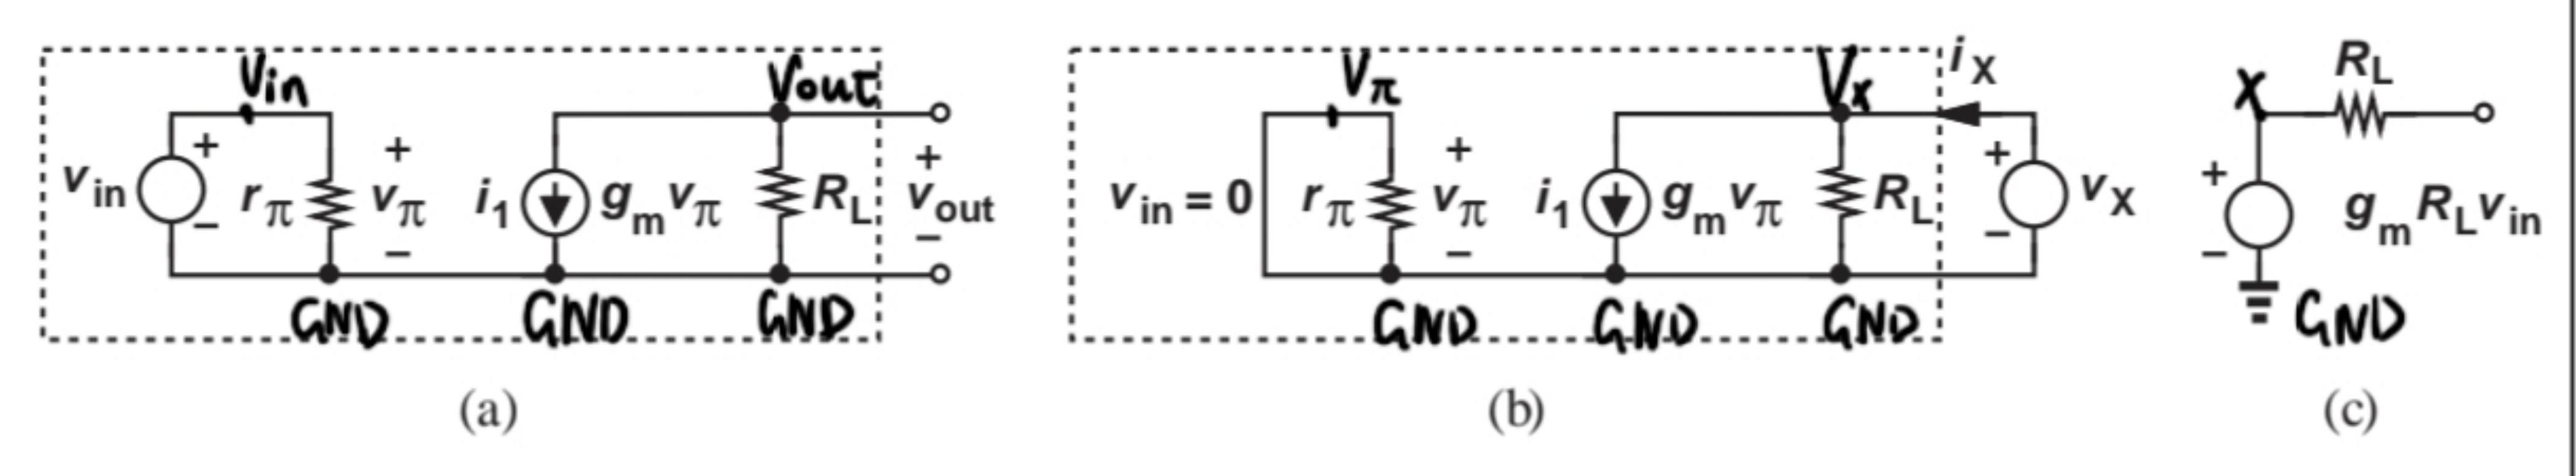
\includegraphics[max width=\textwidth, center]{2024_10_27_cec776a4495ed9df4dfcg-016}

Figure 1.24\\
How do we solve the circuit of Fig. 1.24(b)? We must again eliminate $v_{\pi}$. Fortunately, since both terminals of $r_{\pi}$ are tied to ground, $v_{\pi}=0$ and $g_{m} v_{\pi}=0$. The circuit thus reduces to $R_{L}$ and


\begin{equation*}
i_{X}=\frac{v_{X}}{R_{L}} \tag{1.19}
\end{equation*}


That is,


\begin{equation*}
R_{\mathrm{Thev}}=R_{L} \tag{1.20}
\end{equation*}


Figure 1.24(c) depicts the Thevenin equivalent of the input voltage source and the amplifier. In this case, we call $R_{\text {Thev }}\left(=R_{L}\right)$ the "output impedance" of the circuit.

Exercise Repeat the above example if $r_{\pi} \rightarrow \infty$.

With the Thevenin equivalent of a circuit available, we can readily analyze its behavior in the presence of a subsequent stage or "load."

Example $\quad$ The amplifier of Fig. 1.20 must drive a speaker having an impedance of $R_{s p}$. Determine 1.9 the voltage delivered to the speaker.

Solution Shown in Fig. 1.25(a) is the overall circuit arrangement that we must solve. Replacing the section in the dashed box with its Thevenin equivalent from Fig. 1.24(c), we greatly simplify the circuit [Fig. 1.25(b)], and write


\begin{align*}
v_{\text {out }} & =-g_{m} R_{L} v_{\text {in }} \frac{R_{s p}}{R_{s p}+R_{L}}  \tag{1.21}\\
& =-g_{m} v_{i n}\left(R_{L} \| R_{s p}\right) \tag{1.22}
\end{align*}


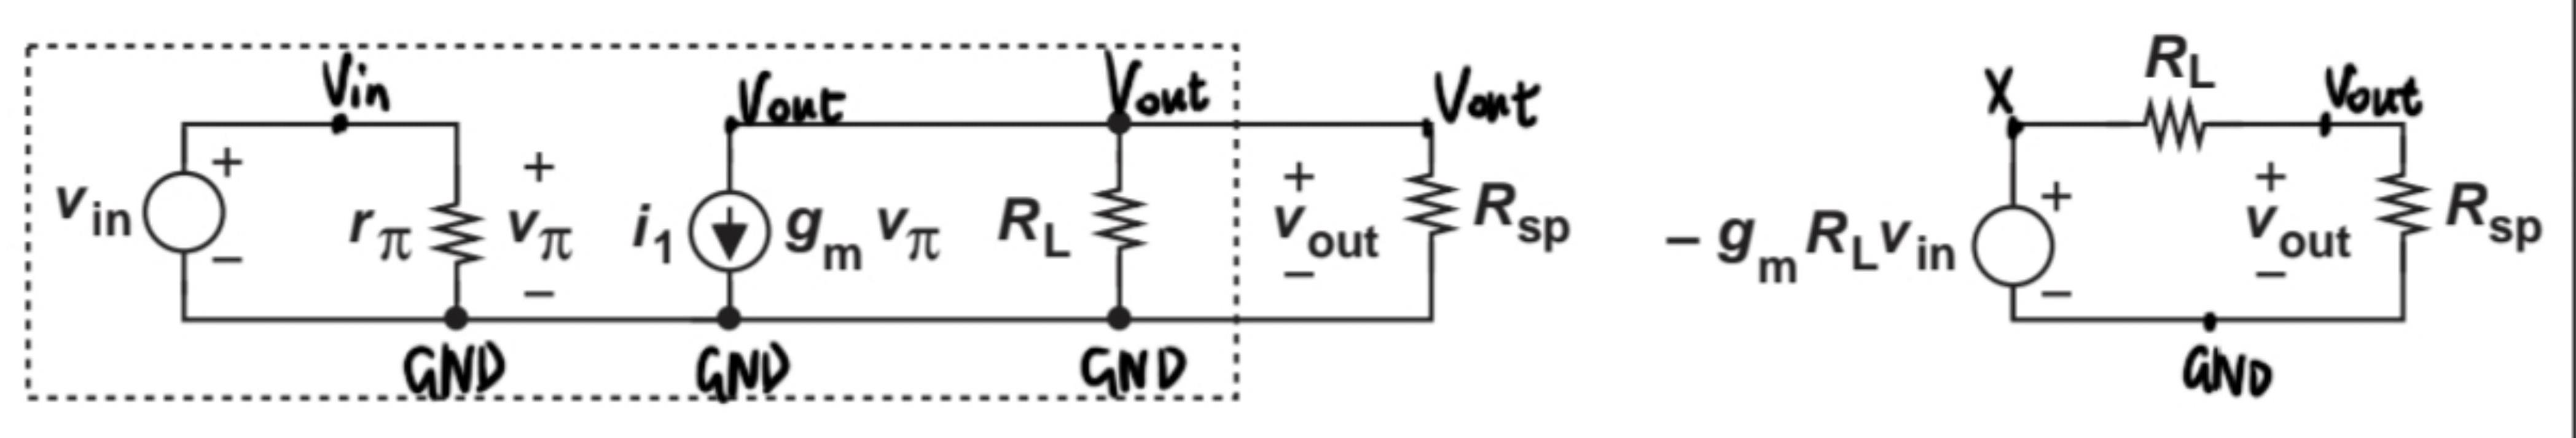
\includegraphics[max width=\textwidth, center]{2024_10_27_cec776a4495ed9df4dfcg-017}\\
(a)\\
(b)

Figure 1.25\\
Exercise Repeat the above example if $r_{\pi} \rightarrow \infty$.

Example\\
1.10

Determine the Thevenin equivalent of the circuit shown in Fig. 1.22 if the output port is of interest.

Solution The open-circuit output voltage is simply obtained from (1.16):


\begin{equation*}
v_{\text {Thev }}=\frac{\left(1+g_{m} r_{\pi}\right) R_{L}}{r_{\pi}+\left(1+g_{m} r_{\pi}\right) R_{L}} v_{i n} \tag{1.23}
\end{equation*}


To calculate the Thevenin impedance, we set $v_{i n}$ to zero and apply a voltage source across the output port as depicted in Fig. 1.26. To eliminate $v_{\pi}$, we recognize that the two terminals of $r_{\pi}$ are tied to those of $v_{X}$ and hence


\begin{equation*}
v_{\pi}=-v_{X} \tag{1.24}
\end{equation*}


\begin{center}
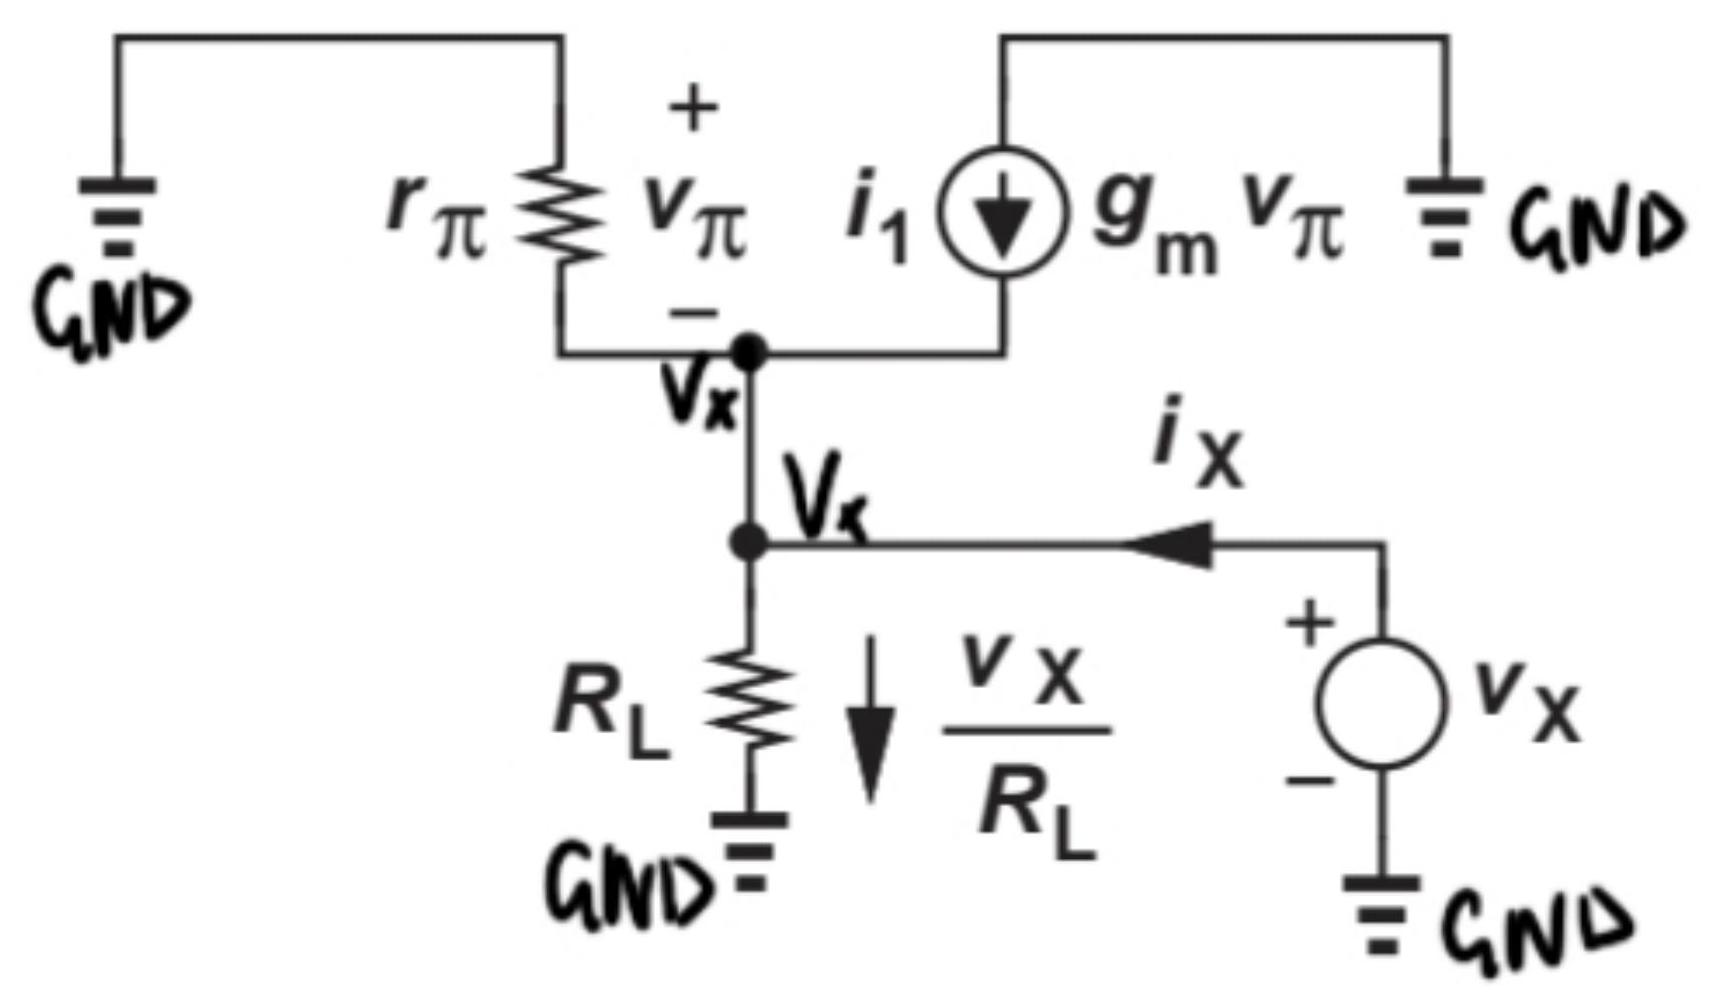
\includegraphics[max width=\textwidth]{2024_10_27_cec776a4495ed9df4dfcg-018}
\end{center}

Figure 1.26\\
We now write a KCL at the output node. The currents $v_{\pi} / r_{\pi}, g_{m} v_{\pi}$, and $i_{X}$ flow into this node and the current $v_{X} / R_{L}$ flows out of it. Consequently,


\begin{equation*}
\frac{v_{\pi}}{r_{\pi}}+g_{m} v_{\pi}+i_{X}=\frac{v_{X}}{R_{L}} \tag{1.25}
\end{equation*}


or


\begin{equation*}
\left(\frac{1}{r_{\pi}}+g_{m}\right)\left(-v_{X}\right)+i_{X}=\frac{v_{X}}{R_{L}} . \tag{1.26}
\end{equation*}


That is,


\begin{align*}
R_{\text {Thev }} & =\frac{v_{X}}{i_{X}}  \tag{1.27}\\
& =\frac{r_{\pi} R_{L}}{r_{\pi}+\left(1+g_{m} r_{\pi}\right) R_{L}} \tag{1.28}
\end{align*}


Exercise What happens if $R_{L}=\infty$ ?

Norton's theorem states that a (linear) one-port network can be represented by one current source in parallel with one impedance (Fig. 1.27). The equivalent current, $i_{\text {Nor }}$, is obtained by shorting the port of interest and computing the current that flows through it. The equivalent impedance, $Z_{\mathrm{Nor}}$, is determined by setting all independent voltage and current sources in the circuit to zero and calculating the impedance seen at the port. Of course, $Z_{\text {Nor }}=Z_{\text {Thev }}$.\\
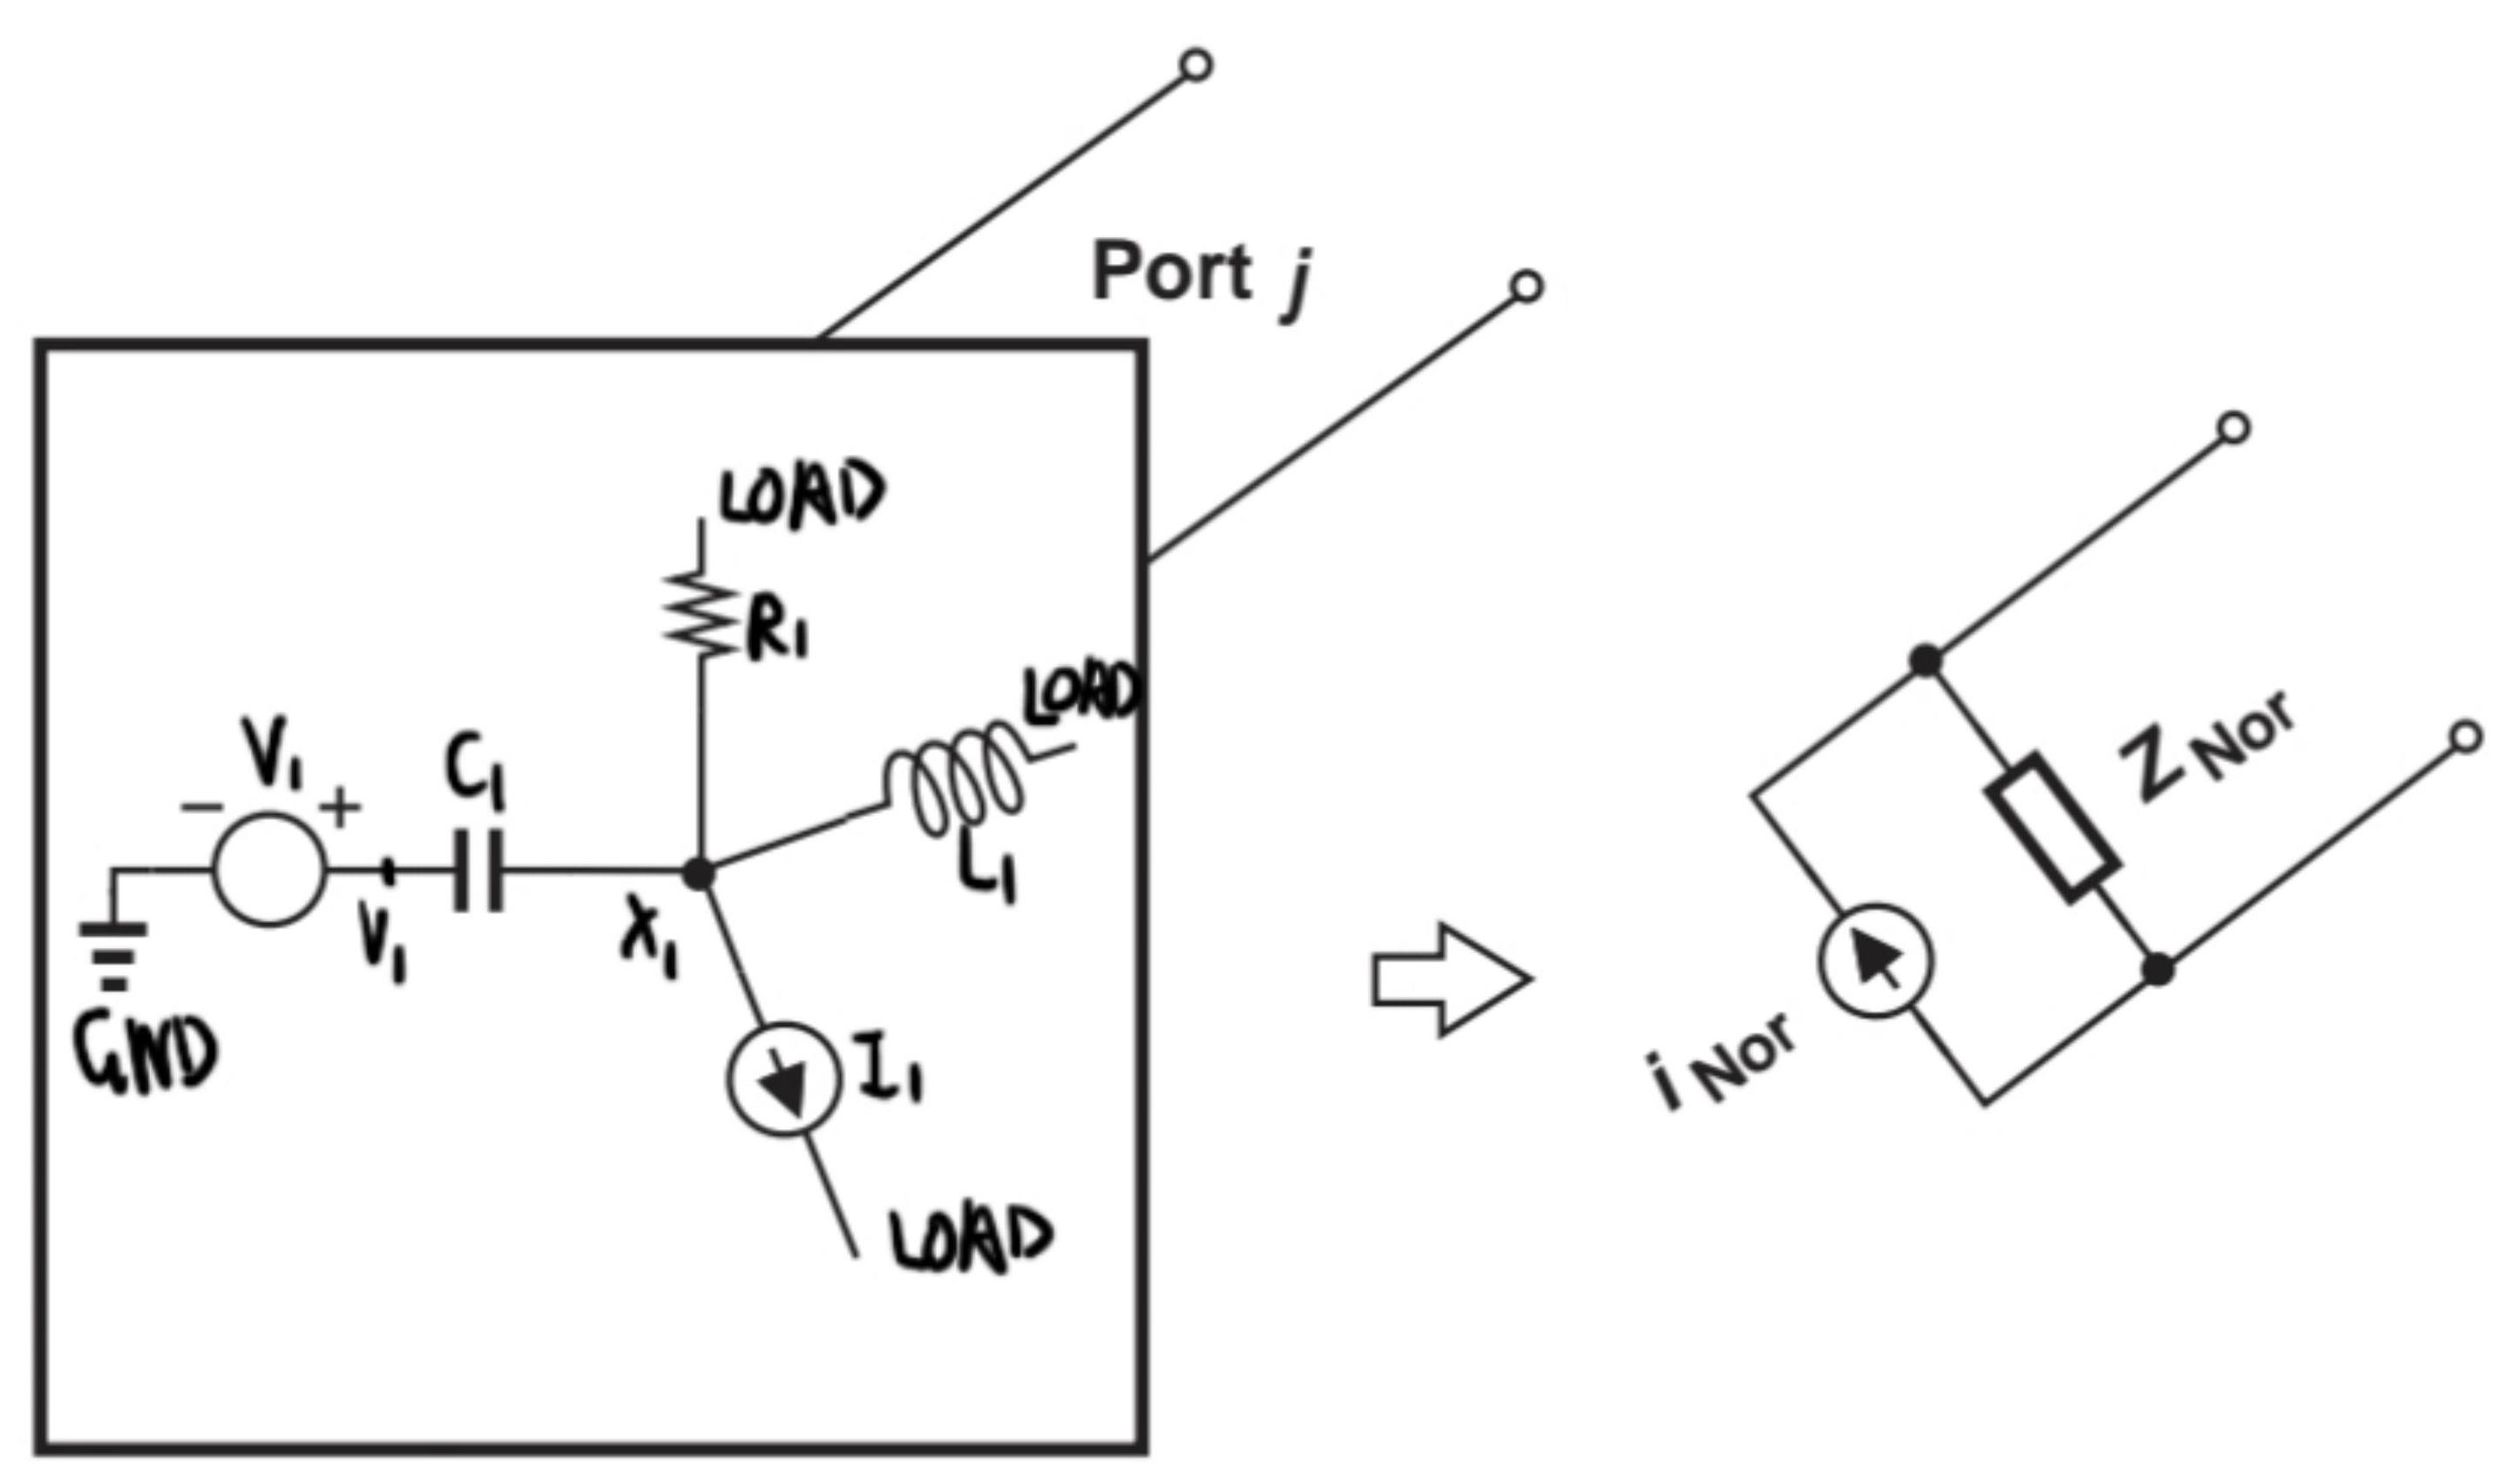
\includegraphics[max width=\textwidth, center]{2024_10_27_cec776a4495ed9df4dfcg-018(1)}

Figure 1.27 Norton's theorem.

\section*{Example}
1.11

Determine the Norton equivalent of the circuit shown in Fig. 1.20 if the output port is of interest.

Solution As depicted in Fig. 1.28(a), we short the output port and seek the value of $i_{\text {Nor }}$. Since the voltage across $R_{L}$ is now forced to zero, this resistor carries no current.\\
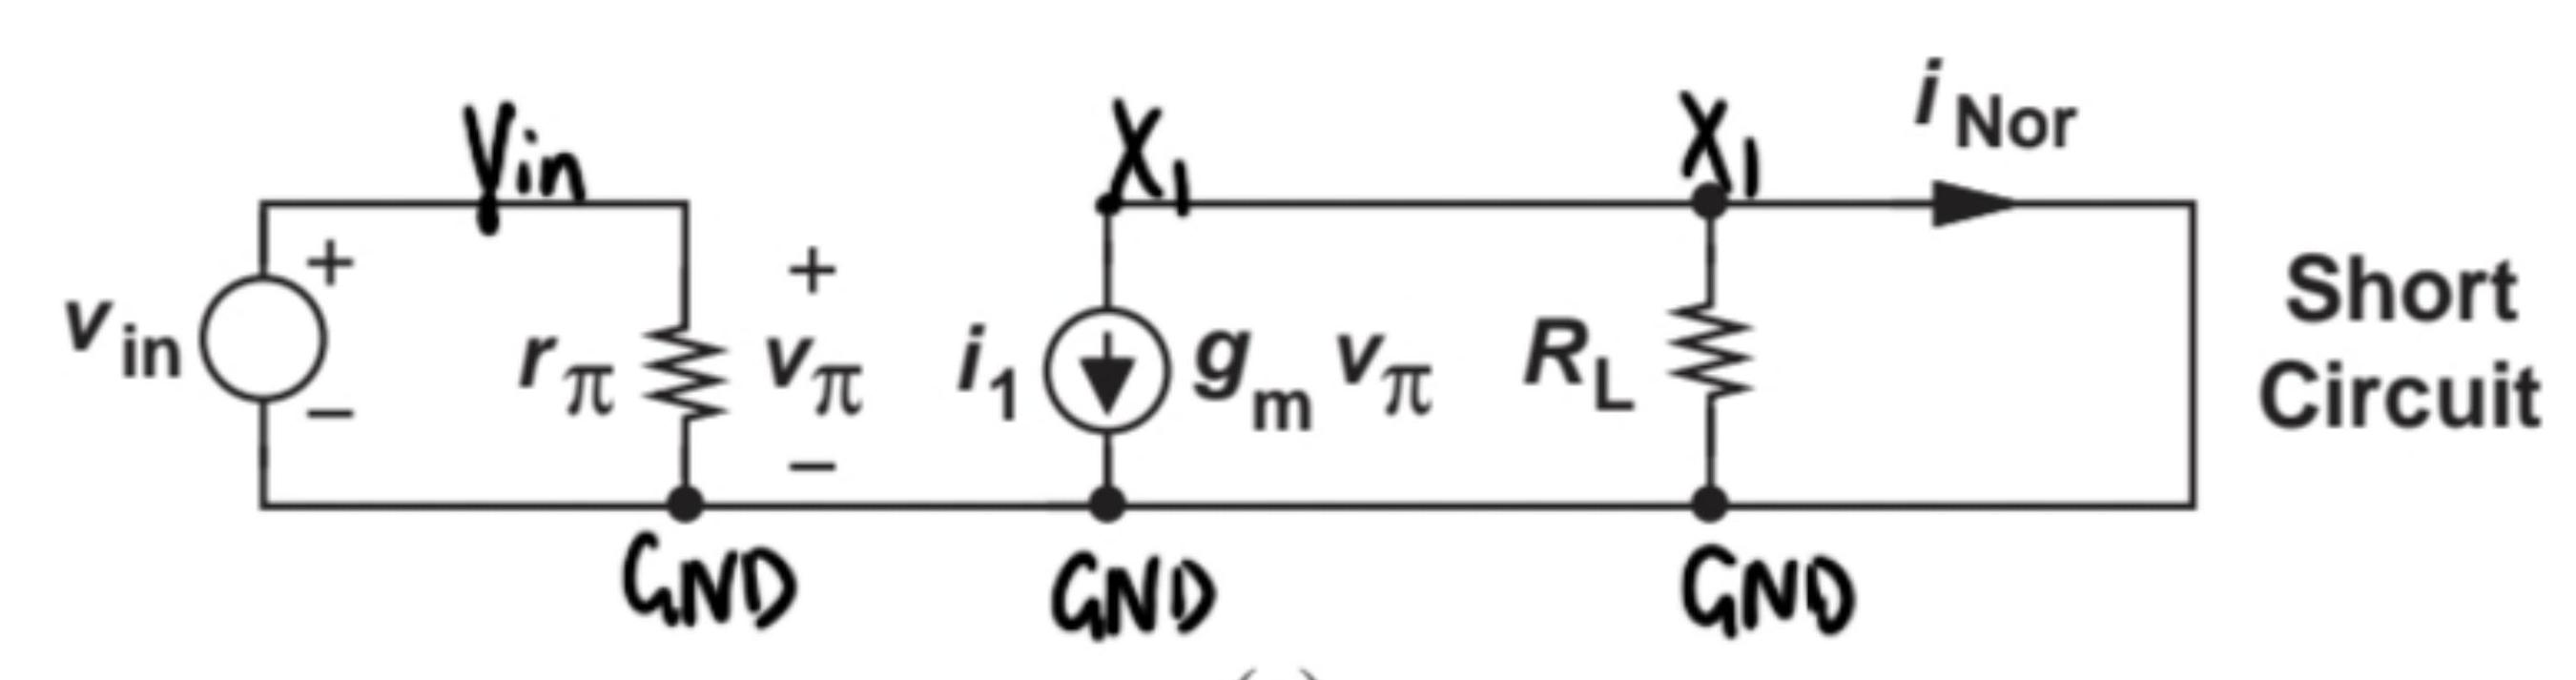
\includegraphics[max width=\textwidth, center]{2024_10_27_cec776a4495ed9df4dfcg-019(1)}\\
(a)\\
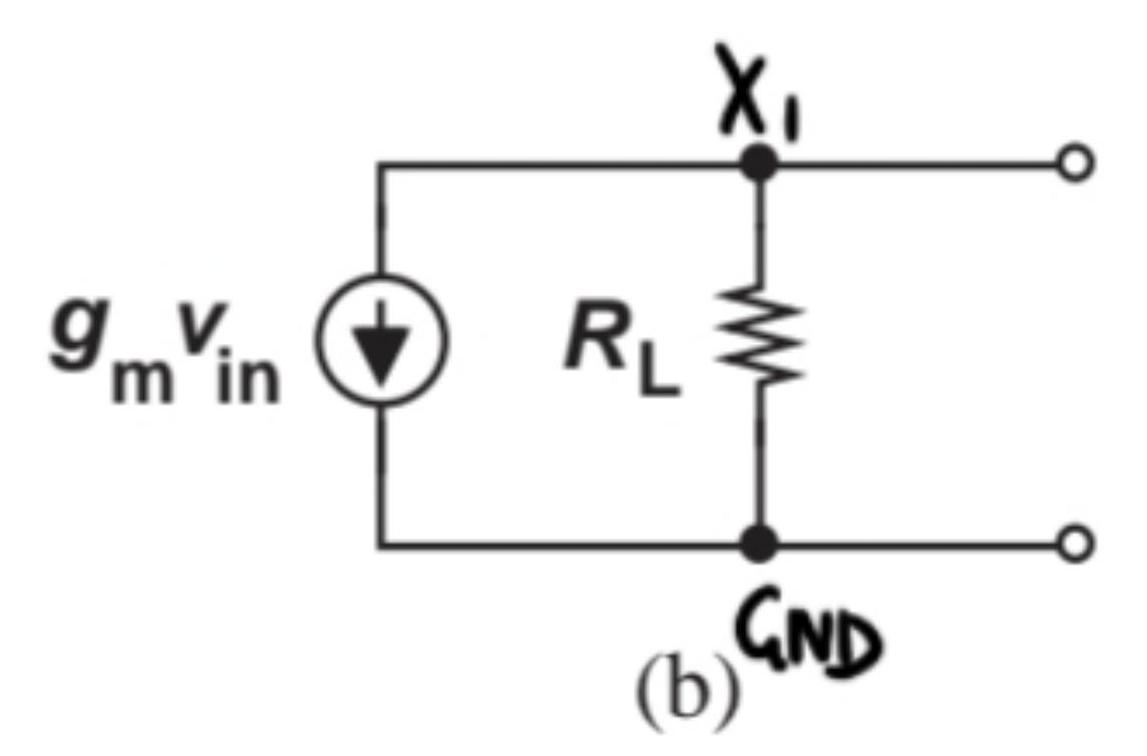
\includegraphics[max width=\textwidth, center]{2024_10_27_cec776a4495ed9df4dfcg-019}

Figure 1.28

A KCL at the output node thus yields


\begin{align*}
i_{\mathrm{Nor}} & =-g_{m} v_{\pi}  \tag{1.29}\\
& =-g_{m} v_{i n} \tag{1.30}
\end{align*}


Also, from Example $1.8, R_{\text {Nor }}\left(=R_{\text {Thev }}\right)=R_{L}$. The Norton equivalent therefore emerges as shown in Fig. 1.28(b). To check the validity of this model, we observe that the flow of $i_{\text {Nor }}$ through $R_{L}$ produces a voltage of $-g_{m} R_{L} v_{i n}$, the same as the output voltage of the original circuit.

Exercise Repeat the above example if a resistor of value $R_{1}$ is added between the top terminal of $v_{\text {in }}$ and the output node.

Determine the Norton equivalent of the circuit shown in Fig. 1.22 if the output port is interest.

Solution Shorting the output port as illustrated in Fig. 1.29(a), we note that $R_{L}$ carries no current. Thus,\\
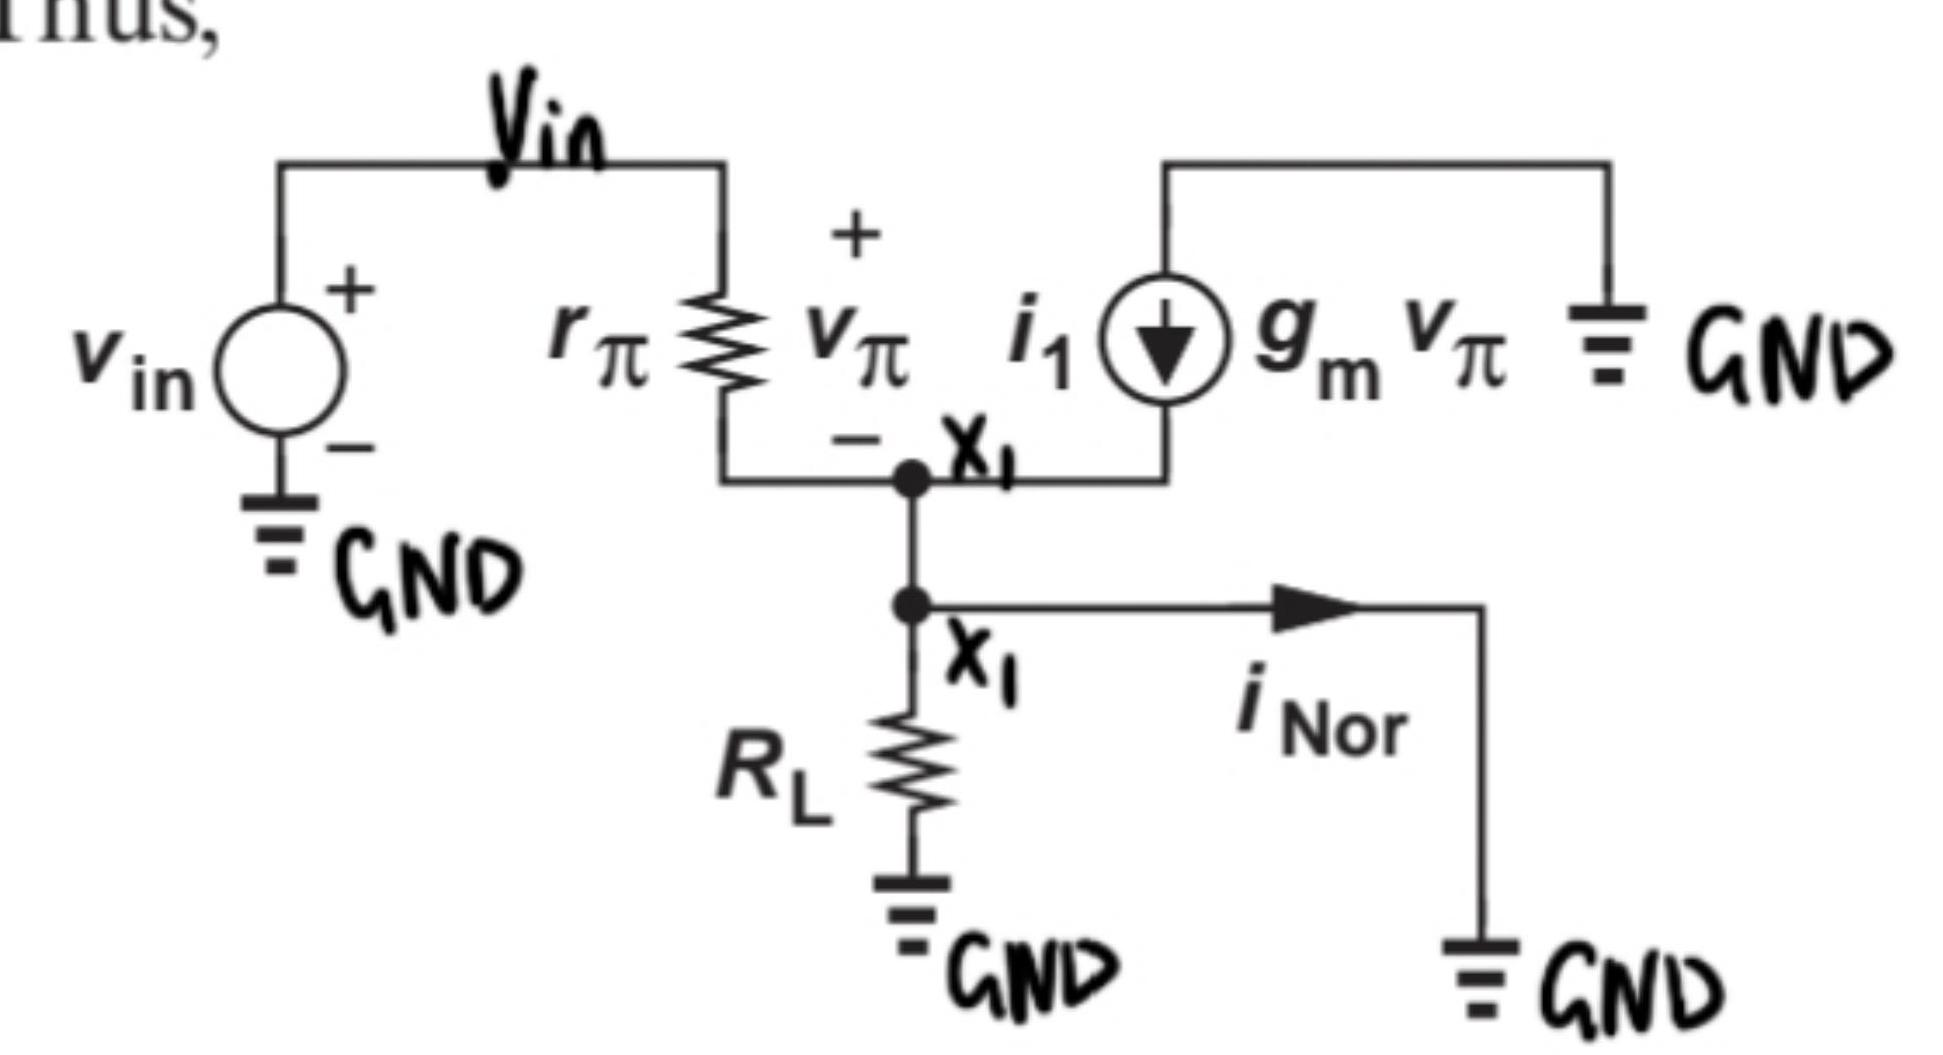
\includegraphics[max width=\textwidth, center]{2024_10_27_cec776a4495ed9df4dfcg-019(3)}\\
(a)\\
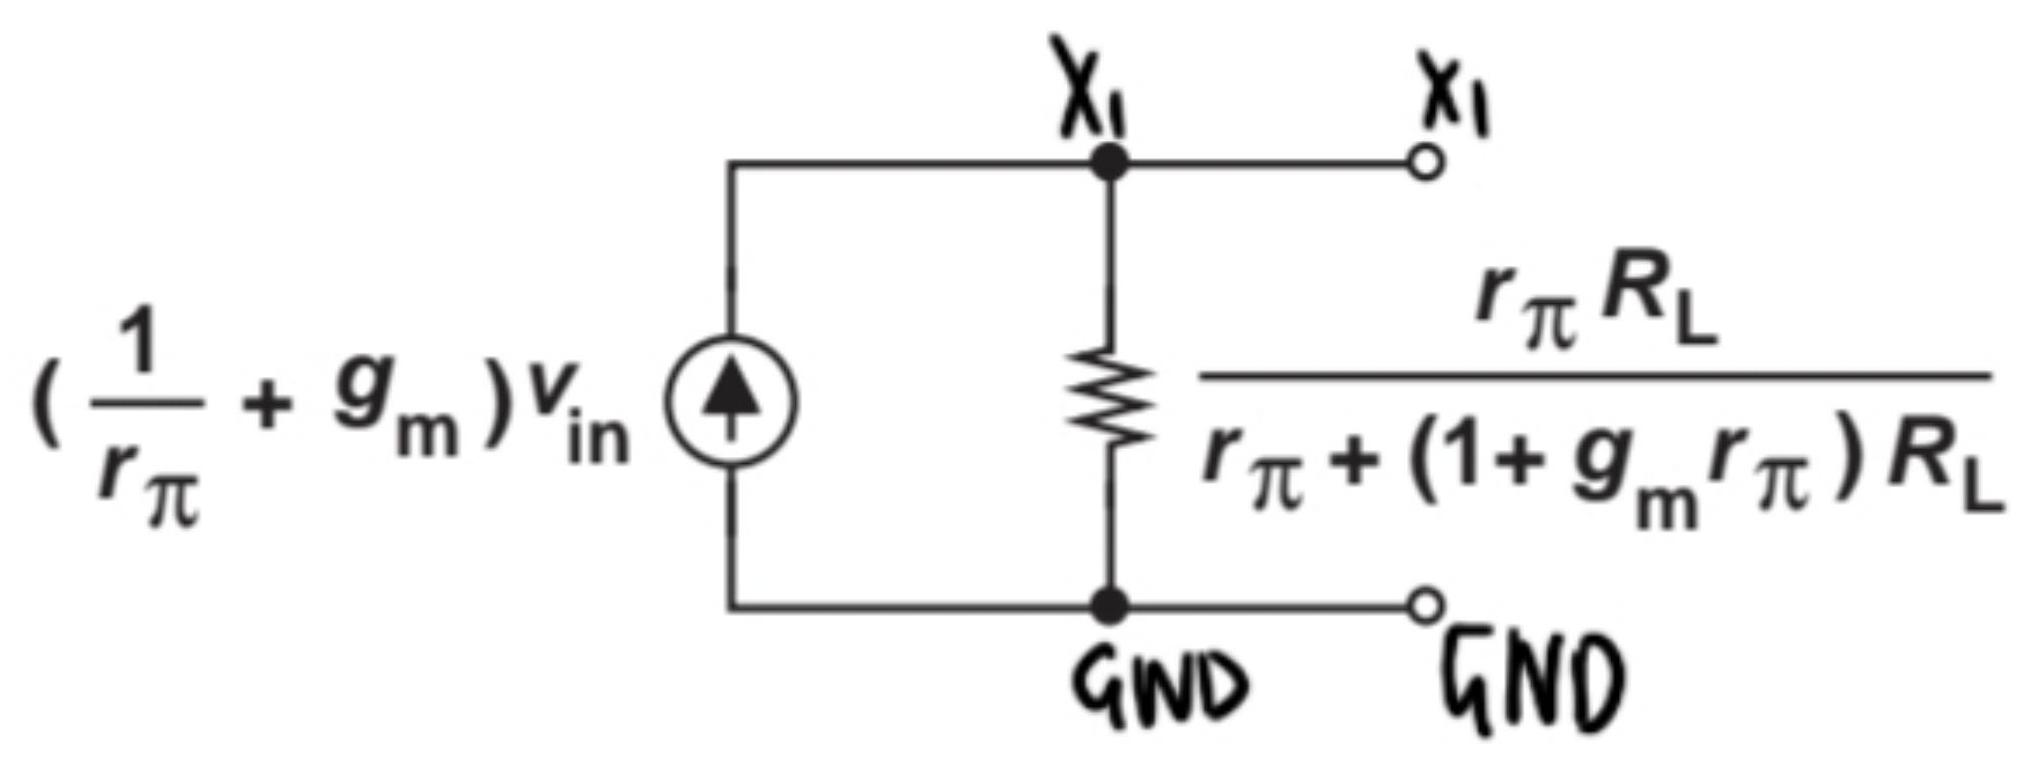
\includegraphics[max width=\textwidth, center]{2024_10_27_cec776a4495ed9df4dfcg-019(2)}\\
(b)

Figure 1.29


\begin{equation*}
i_{\mathrm{Nor}}=\frac{v_{\pi}}{r_{\pi}}+g_{m} v_{\pi} \tag{1.31}
\end{equation*}


Also, $v_{i n}=v_{\pi}$ (why?), yielding


\begin{equation*}
i_{\text {Nor }}=\left(\frac{1}{r_{\pi}}+g_{m}\right) v_{i n} \tag{1.32}
\end{equation*}


With the aid of $R_{T h e v}$ found in Example 1.10, we construct the Norton equivalent depicted in Fig. 1.29(b).

Exercise What happens if $r_{\pi}=\infty$ ?

\subsection*{1.4 CHAPTER SUMMARY}
\begin{itemize}
  \item Electronic functions appear in many devices, including cellphones, digital cameras, laptop computers, etc.
  \item Amplification is an essential operation in many analog and digital systems.
  \item Analog circuits process signals that can assume various values at any time. By contrast, digital circuits deal with signals having only two levels and switching between these values at known points in time.
  \item Despite the "digital revolution," analog circuits find wide application in most of today's electronic systems.
  \item The voltage gain of an amplifier is defined as $v_{\text {out }} / v_{i n}$ and sometimes expressed in decibels $(\mathrm{dB})$ as $20 \log \left(v_{\text {out }} / v_{\text {in }}\right)$.
  \item Kirchoff's current law (KCL) states that the sum of all currents flowing into any node is zero. Kirchoff's voltage law (KVL) states that the sum of all voltages around any loop is zero.
  \item Norton's theorem allows simplifying a one-port circuit to a current source in parallel with an impedance. Similarly, Thevenin's theorem reduces a one-port circuit to a voltage source in series with an impedance.\\
\includegraphics[max width=\textwidth, center]{2024_10_27_cec776a4495ed9df4dfcg-021}
\end{itemize}

\section*{Basic Physics of Semiconductors}
Microelectronic circuits are based on complex semiconductor structures that have been under active research for the past six decades. While this book deals with the analysis and design of circuits, we should emphasize at the outset that a good understanding of devices is essential to our work. The situation is similar to many other engineering problems, e.g., one cannot design a high-performance automobile without a detailed knowledge of the engine and its limitations.

Nonetheless, we do face a dilemma. Our treatment of device physics must contain enough depth to provide adequate understanding, but must also be sufficiently brief to allow quick entry into circuits. This chapter accomplishes this task.

Our ultimate objective in this chapter is to study a fundamentally important and versatile device called the "diode." However, just as we need to eat our broccoli before having dessert, we must develop a basic understanding of "semiconductor" materials and their current conduction mechanisms before attacking diodes.

In this chapter, we begin with the concept of semiconductors and study the movement of charge (i.e., the flow of current) in them. Next, we deal with the " $p n$ junction," which also serves as diode, and formulate its behavior. Our ultimate goal is to represent the device by a circuit model (consisting of resistors, voltage or current sources, capacitors, etc.), so that a circuit using such a device can be analyzed easily. The outline is shown below.

\section*{Semiconductors}
\begin{itemize}
  \item Charge Carriers
  \item Doping
  \item Transport of Carriers
\end{itemize}

\section*{PN Junction}
\begin{itemize}
  \item Structure
  \item Reverse and Forward Bias Conditions
  \item I/V Characteristics
  \item Circuit Models
\end{itemize}

It is important to note that the task of developing accurate models proves critical for all microelectronic devices. The electronics industry continues to place greater demands\\
on circuits, calling for aggressive designs that push semiconductor devices to their limits. Thus, a good understanding of the internal operation of devices is necessary. ${ }^{1}$

\subsection*{2.1 SEMICONDUCTOR MATERIALS AND THEIR PROPERTIES}
Since this section introduces a multitude of concepts, it is useful to bear a general outline in mind:\\
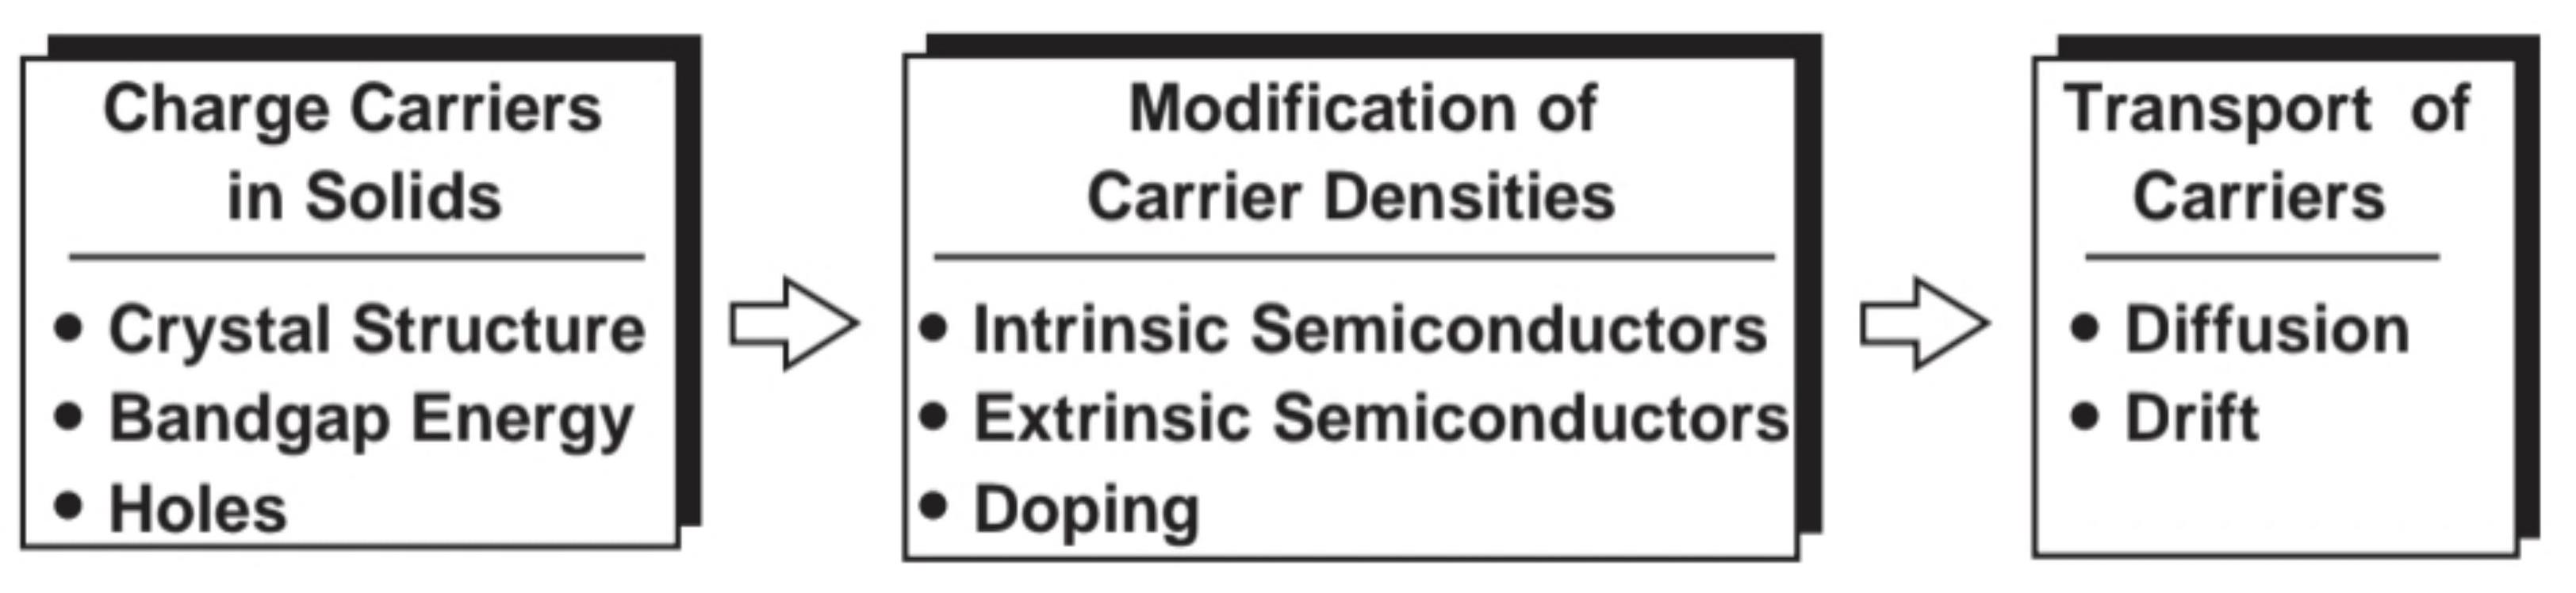
\includegraphics[max width=\textwidth, center]{2024_10_27_cec776a4495ed9df4dfcg-022}

Figure 2.1 Outline of this section.\\
This outline represents a logical thought process: (a) we identify charge carriers in solids and formulate their role in current flow; (b) we examine means of modifying the density of charge carriers to create desired current flow properties; (c) we determine current flow mechanisms. These steps naturally lead to the computation of the current/voltage $(\mathrm{I} / \mathrm{V})$ characteristics of actual diodes in the next section.

\subsection*{2.1.1 Charge Carriers in Solids}
Recall from basic chemistry that the electrons in an atom orbit the nucleus in different "shells." The atom's chemical activity is determined by the electrons in the outermost shell, called "valence" electrons, and how complete this shell is. For example, neon exhibits a complete outermost shell (with eight electrons) and hence no tendency for chemical reactions. On the other hand, sodium has only one valence electron, ready to relinquish it, and chloride has seven valence electrons, eager to receive one more. Both elements are therefore highly reactive.

The above principles suggest that atoms having approximately four valence electrons fall somewhere between inert gases and highly volatile elements, possibly displaying interesting chemical and physical properties. Shown in Fig. 2.2 is a section of the periodic table containing a number of elements with three to five valence electrons. As the most popular material in microelectronics, silicon merits a detailed analysis. ${ }^{2}$

Covalent Bonds A silicon atom residing in isolation contains four valence electrons [Fig. 2.3(a)], requiring another four to complete its outermost shell. If processed properly, the silicon material can form a "crystal" wherein each atom is surrounded by exactly four others [Fig. 2.3(b)]. As a result, each atom shares one valence electron with its neighbors, thereby completing its own shell and those of the neighbors. The "bond" thus formed between atoms is called a "covalent bond" to emphasize the sharing of valence electrons.

The uniform crystal depicted in Fig. 2.3(b) plays a crucial role in semiconductor devices. But, does it carry current in response to a voltage? At temperatures near absolute zero,

\footnotetext{${ }^{1}$ As design managers often say, "If you do not push the devices and circuits to their limit but your competitor does, then you lose to your competitor."\\
${ }^{2}$ Silicon is obtained from sand after a great deal of processing.
}
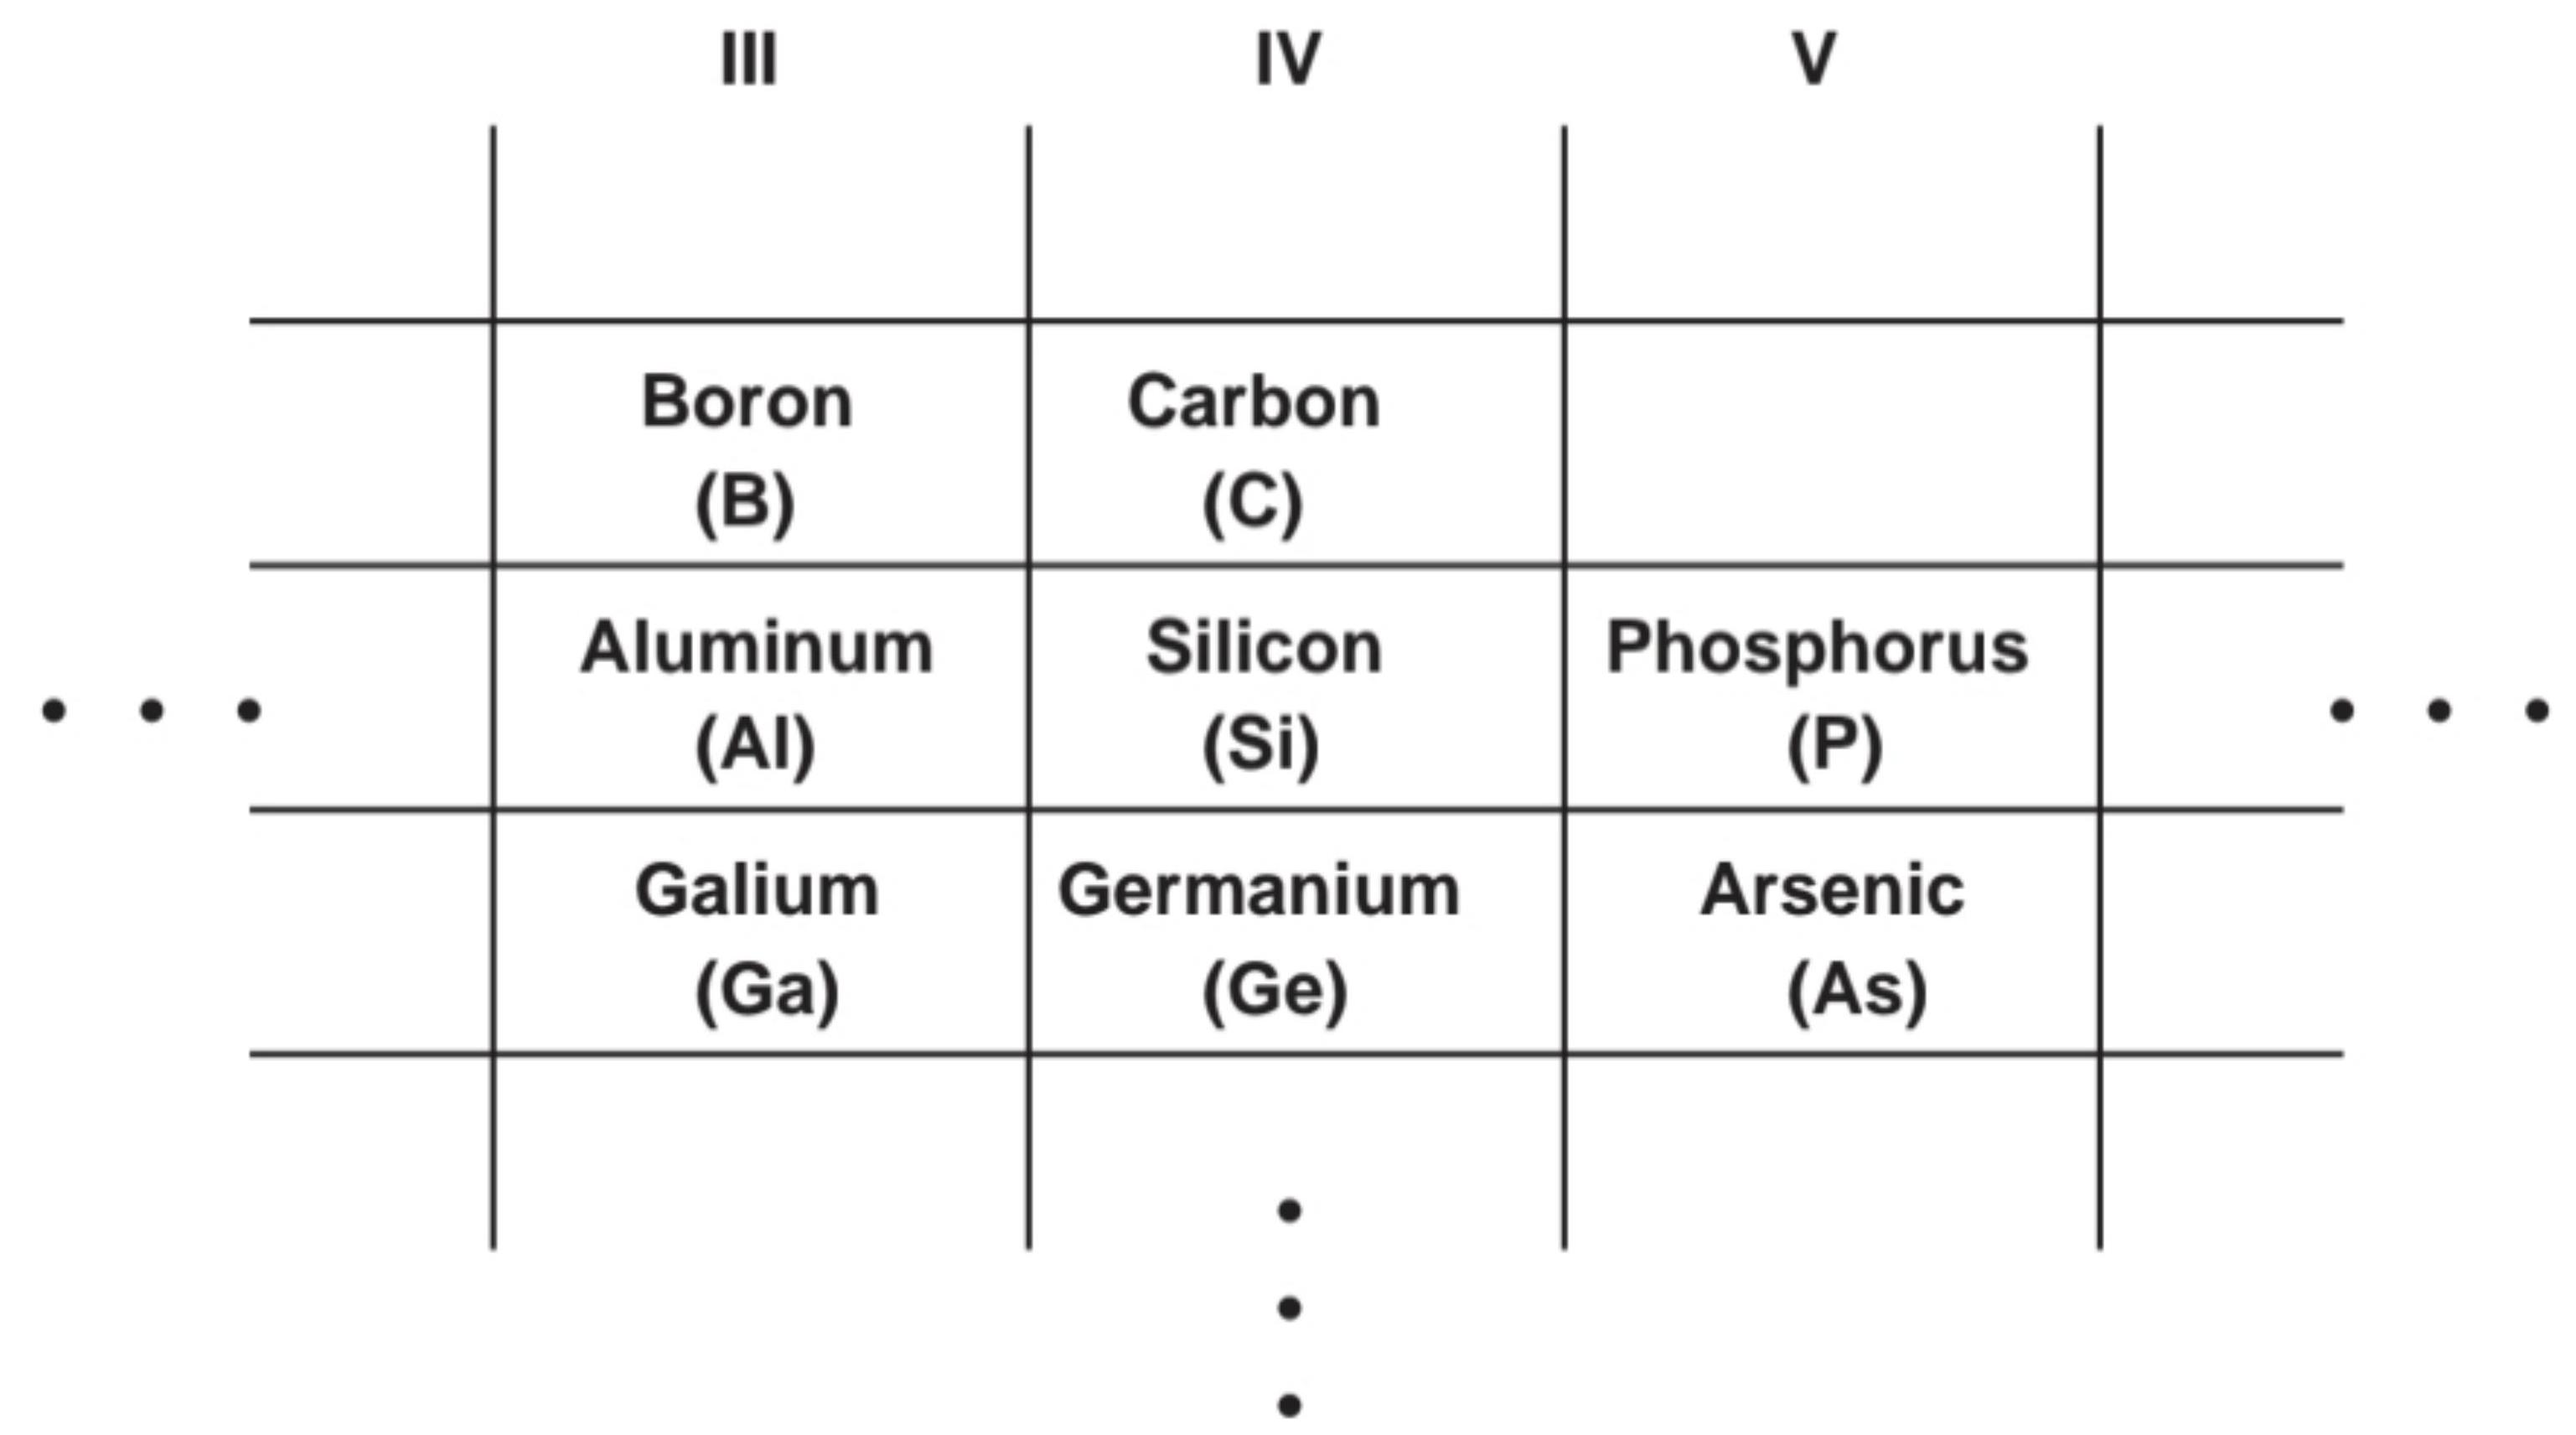
\includegraphics[max width=\textwidth, center]{2024_10_27_cec776a4495ed9df4dfcg-023(2)}

Figure 2.2 Section of the periodic table.\\
the valence electrons are confined to their respective covalent bonds, refusing to move freely. In other words, the silicon crystal behaves as an insulator for $T \rightarrow 0 K$. However, at higher temperatures, electrons gain thermal energy, occasionally breaking away from the bonds and acting as free charge carriers [Fig. 2.3(c)] until they fall into another incomplete bond. We will hereafter use the term "electrons" to refer to free electrons.\\
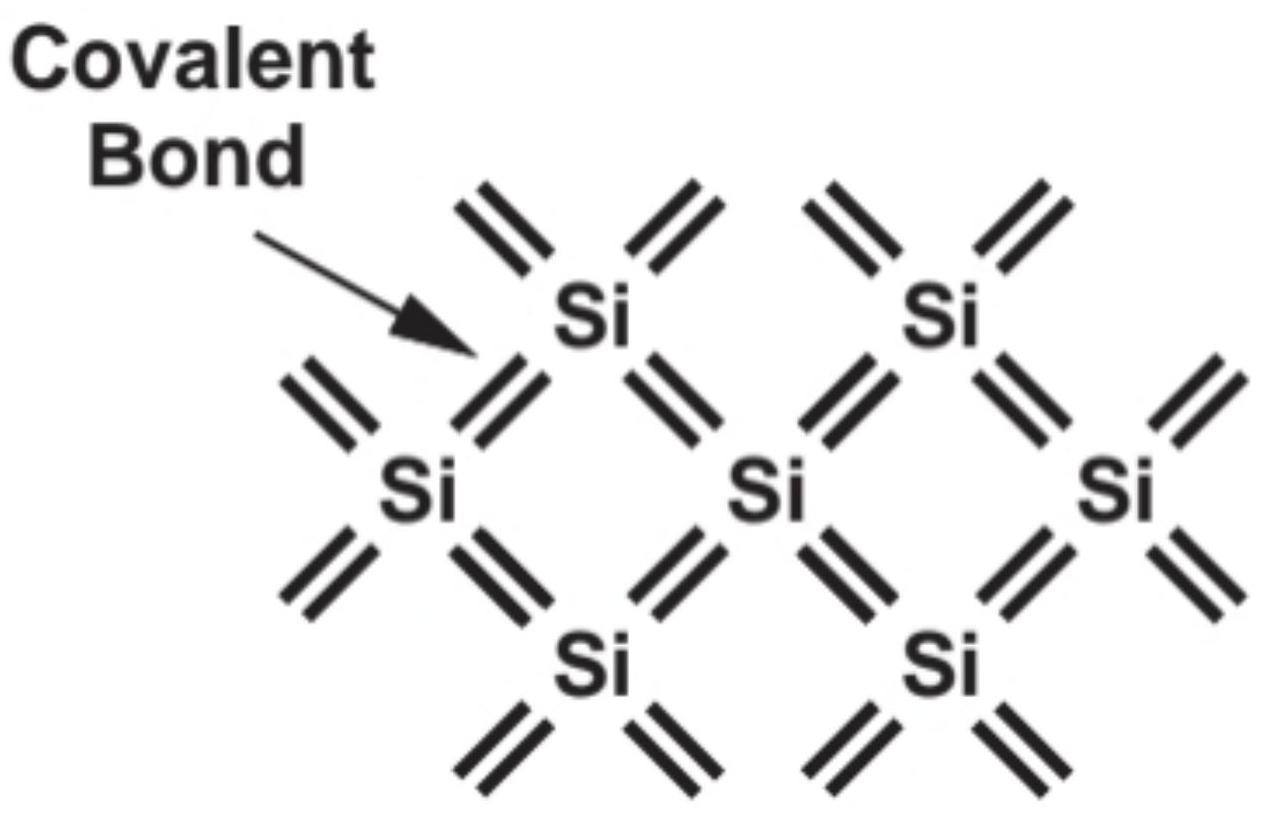
\includegraphics[max width=\textwidth, center]{2024_10_27_cec776a4495ed9df4dfcg-023(1)}\\
(b)\\
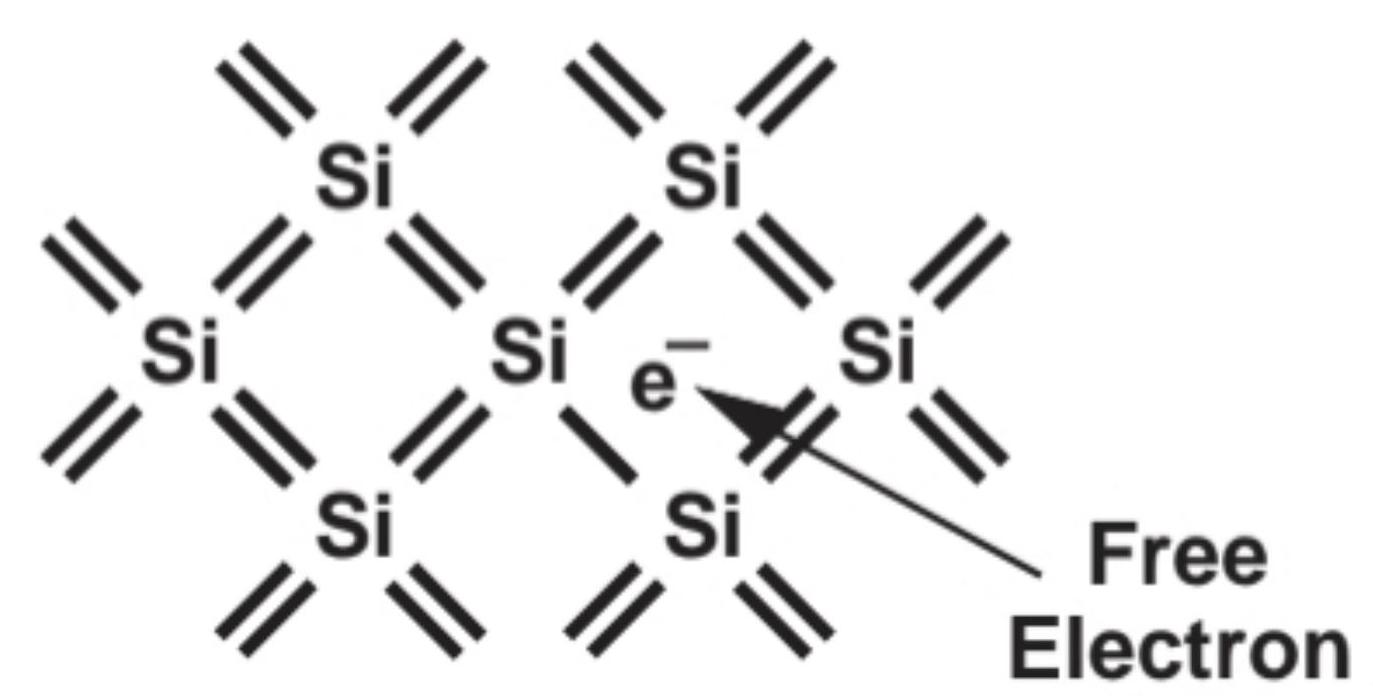
\includegraphics[max width=\textwidth, center]{2024_10_27_cec776a4495ed9df4dfcg-023}\\
(c)

Figure 2.3 (a) Silicon atom, (b) covalent bonds between atoms, (c) free electron released by thermal energy.

Holes When freed from a covalent bond, an electron leaves a "void" behind because the bond is now incomplete. Called a "hole," such a void can readily absorb a free electron if one becomes available. Thus, we say an "electron-hole pair" is generated when an electron is freed, and an "electron-hole recombination" occurs when an electron "falls" into a hole.

Why do we bother with the concept of the hole? After all, it is the free electron that actually moves in the crystal. To appreciate the usefulness of holes, consider the time evolution illustrated in Fig. 2.4. Suppose covalent bond number 1 contains a hole after\\
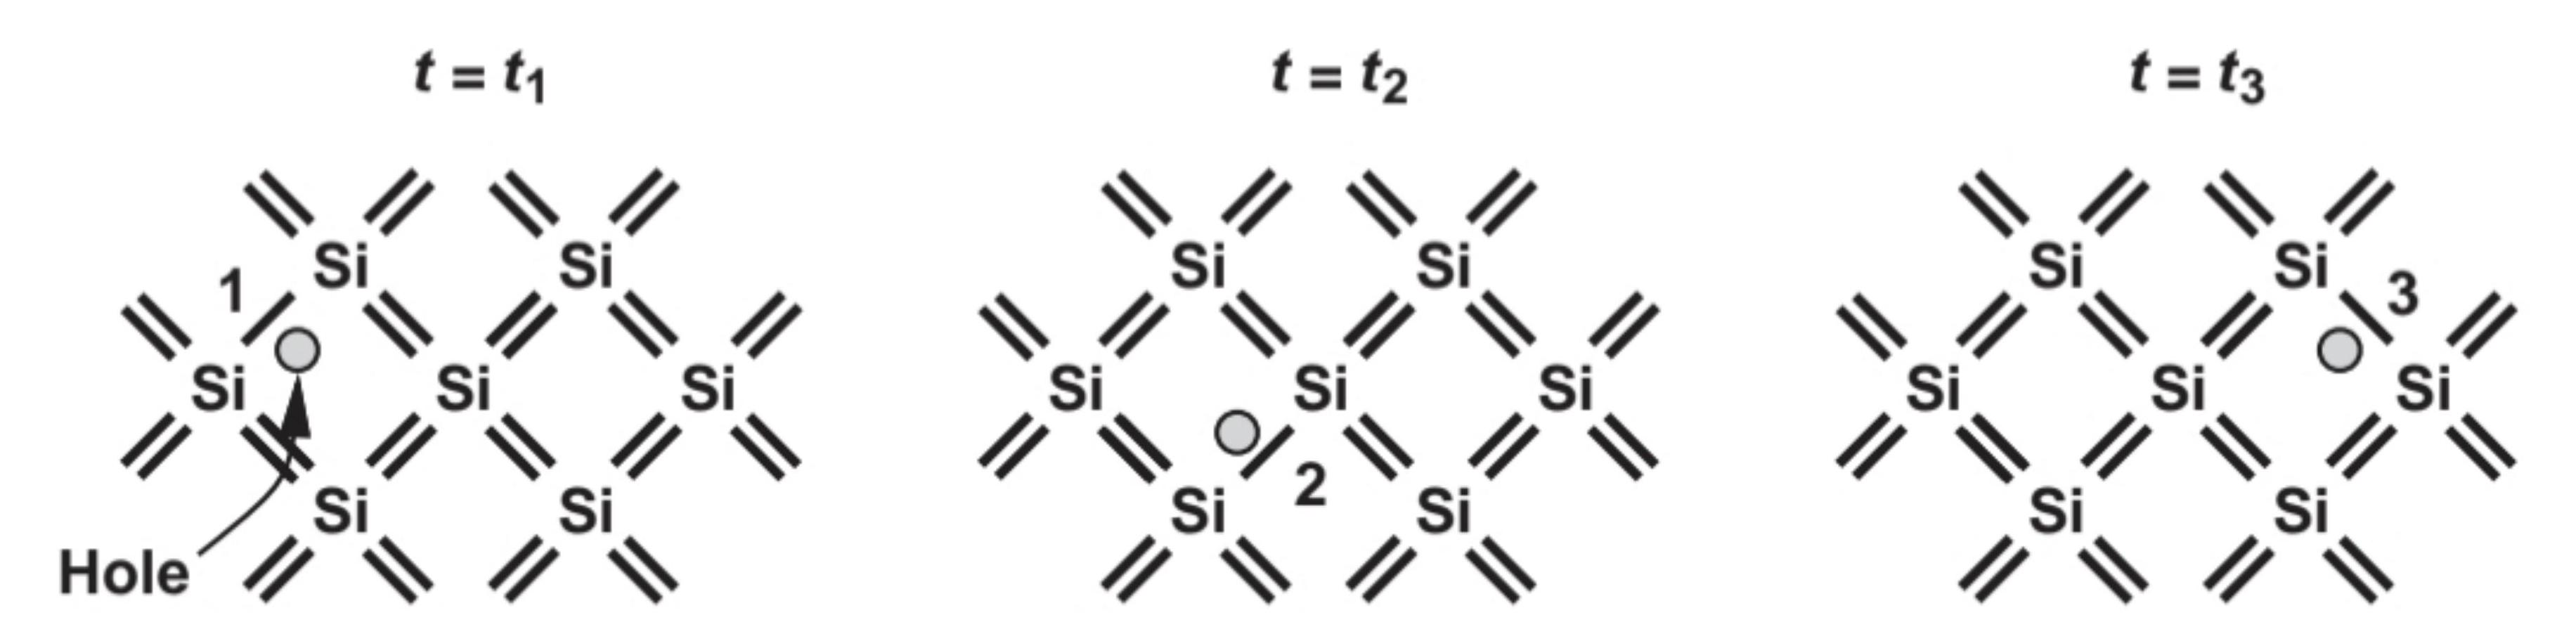
\includegraphics[max width=\textwidth, center]{2024_10_27_cec776a4495ed9df4dfcg-023(3)}

Figure 2.4 Movement of electron through crystal.\\
losing an electron some time before $t=t_{1}$. At $t=t_{2}$, an electron breaks away from bond number 2 and recombines with the hole in bond number 1. Similarly, at $t=t_{3}$, an electron leaves bond number 3 and falls into the hole in bond number 2. Looking at the three "snapshots," we can say one electron has traveled from right to left, or, alternatively, one hole has moved from left to right. This view of current flow by holes proves extremely useful in the analysis of semiconductor devices.

Bandgap Energy We must now answer two important questions. First, does any thermal energy create free electrons (and holes) in silicon? No, in fact, a minimum energy is required to dislodge an electron from a covalent bond. Called the "bandgap energy" and denoted by $E_{g}$, this minimum is a fundamental property of the material. For silicon, $E_{g}=1.12 \mathrm{eV}^{3}$

The second question relates to the conductivity of the material and is as follows. How many free electrons are created at a given temperature? From our observations thus far, we postulate that the number of electrons depends on both $E_{g}$ and $T$ : a greater $E_{g}$ translates to fewer electrons, but a higher $T$ yields more electrons. To simplify future derivations, we consider the density (or concentration) of electrons, i.e., the number of electrons per unit volume, $n_{i}$, and write for silicon:


\begin{equation*}
n_{i}=5.2 \times 10^{15} T^{3 / 2} \exp \frac{-E_{g}}{2 k T} \text { electrons } / \mathrm{cm}^{3} \tag{2.1}
\end{equation*}


where $k=1.38 \times 10^{-23} \mathrm{~J} / \mathrm{K}$ is called the Boltzmann constant. The derivation can be found in books on semiconductor physics, e.g., [1]. As expected, materials having a larger $E_{g}$ exhibit a smaller $n_{i}$. Also, as $T \rightarrow 0$, so do $T^{3 / 2}$ and $\exp \left[-E_{g} /(2 k T)\right]$, thereby bringing $n_{i}$ toward zero.

The exponential dependence of $n_{i}$ upon $E_{g}$ reveals the effect of the bandgap energy on the conductivity of the material. Insulators display a high $E_{g}$; for example, $E_{g}=2.5 \mathrm{eV}$ for diamond. Conductors, on the other hand, have a small bandgap. Finally, semiconductors exhibit a moderate $E_{g}$, typically ranging from 1 eV to 1.5 eV .

Example Determine the density of electrons in silicon at $T=300 \mathrm{~K}$ (room temperature) and 2.1 $T=600 \mathrm{~K}$.

Solution Since $E_{g}=1.12 \mathrm{eV}=1.792 \times 10^{-19} \mathrm{~J}$, we have


\begin{align*}
& n_{i}(T=300 \mathrm{~K})=1.08 \times 10^{10} \text { electrons } / \mathrm{cm}^{3}  \tag{2.2}\\
& n_{i}(T=600 \mathrm{~K})=1.54 \times 10^{15} \text { electrons } / \mathrm{cm}^{3} \tag{2.3}
\end{align*}


Since for each free electron, a hole is left behind, the density of holes is also given by (2.2) and (2.3).

Exercise Repeat the above exercise for a material having a bandgap of 1.5 eV .

The $n_{i}$ values obtained in the above example may appear quite high, but, noting that silicon has $5 \times 10^{22}$ atoms $/ \mathrm{cm}^{3}$, we recognize that only one in $5 \times 10^{12}$ atoms benefit from a

\footnotetext{${ }^{3}$ The unit eV (electron volt) represents the energy necessary to move one electron across a potential difference of 1 V . Note that $1 \mathrm{eV}=1.6 \times 10^{-19} \mathrm{~J}$.
}
\includegraphics[max width=\textwidth, center]{2024_10_27_cec776a4495ed9df4dfcg-025(1)}\\
2.1 Semiconductor Materials and Their Properties\\
free electron at room temperature. In other words, silicon still seems a very poor conductor. But, do not despair! We next introduce a means of making silicon more useful.

\subsection*{2.1.2 Modification of Carrier Densities}
Intrinsic and Extrinsic Semiconductors The "pure" type of silicon studied thus far is an example of "intrinsic semiconductors," suffering from a very high resistance. Fortunately, it is possible to modify the resistivity of silicon by replacing some of the atoms in the crystal with atoms of another material. In an intrinsic semiconductor, the electron density, $n\left(=n_{i}\right)$, is equal to the hole density, $p$. Thus,

\section*{Did you know?}
The semiconductor industry manufactures microprocessors, memories, RF transceivers, imaging chips, and many other products, bringing in an annual revenue of 300 billion dollars. This means that, of the seven billion people in the world, each person spends an average of about $\$ 40$ on semiconductor chips every year. This starts when children buy their first video game device.


\begin{equation*}
n p=n_{i}^{2} \tag{2.4}
\end{equation*}


We return to this equation later.\\
Recall from Fig. 2.2 that phosphorus ( P ) contains five valence electrons. What happens if some P atoms are introduced in a silicon crystal? As illustrated in Fig. 2.5, each P atom shares four electrons with the neighboring silicon atoms, leaving the fifth electron "unattached." This electron is free to move, serving as a charge carrier. Thus, if $N$ phosphorus atoms are uniformly introduced in each cubic centimeter of a silicon crystal, then the density of free electrons rises by the same amount.\\
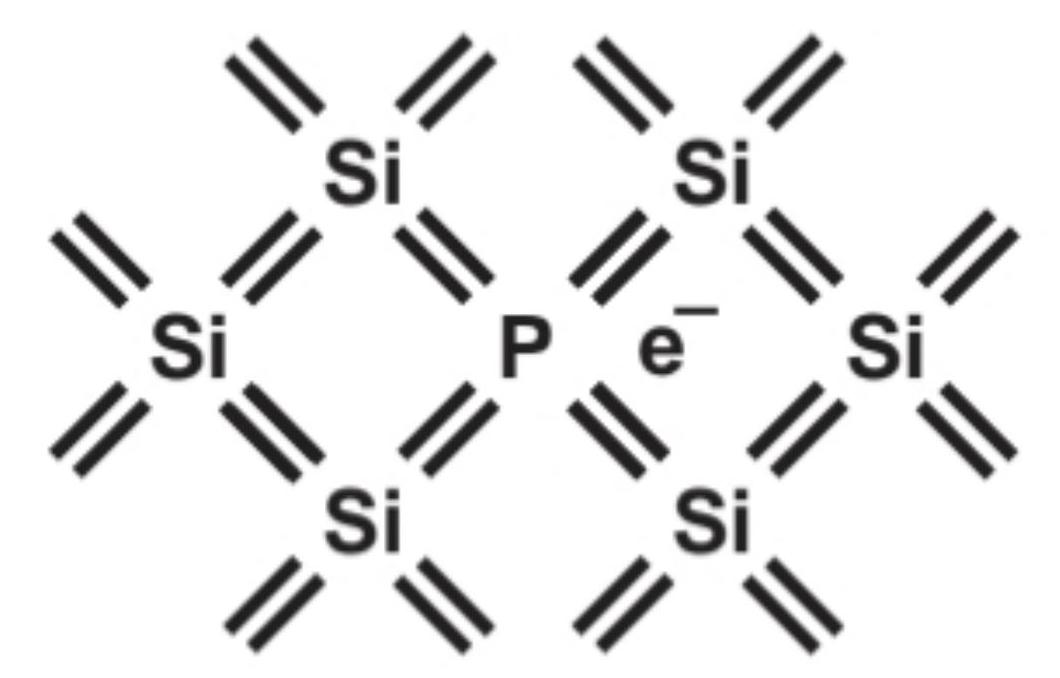
\includegraphics[max width=\textwidth, center]{2024_10_27_cec776a4495ed9df4dfcg-025}

Figure 2.5 Loosely-attached electon with phosphorus doping.

The controlled addition of an "impurity" such as phosphorus to an intrinsic semiconductor is called "doping," and phosphorus itself a "dopant." Providing many more free electrons than in the intrinsic state, the doped silicon crystal is now called "extrinsic," more specifically, an " $n$-type" semiconductor to emphasize the abundance of free electrons.

As remarked earlier, the electron and hole densities in an intrinsic semiconductor are equal. But, how about these densities in a doped material? It can be proved that even in this case,


\begin{equation*}
n p=n_{i}^{2} \tag{2.5}
\end{equation*}


where $n$ and $p$ respectively denote the electron and hole densities in the extrinsic semiconductor. The quantity $n_{i}$ represents the densities in the intrinsic semiconductor (hence the subscript $i$ ) and is therefore independent of the doping level [e.g., Eq. (2.1) for silicon].

Solution Equation (2.5) reveals that $p$ must fall below its intrinsic level as more $n$-type dopants are added to the crystal. This occurs because many of the new electrons donated by the dopant "recombine" with the holes that were created in the intrinsic material.

Exercise Why can we not say that $n+p$ should remain constant?

\begin{center}
\begin{tabular}{|c|c|}
\hline
\( \left\lvert\, \begin{gathered} \text { Example } \\ 2.3 \end{gathered}\right. \) & A piece of crystalline silicon is doped uniformly with phosphorus atoms. The doping density is $10^{16}$ atoms $/ \mathrm{cm}^{3}$. Determine the electron and hole densities in this material at the room temperature. \\
\hline
\multirow[t]{5}{*}{Solution} & The addition of $10^{16} \mathrm{P}$ atoms introduces the same number of free electrons per cubic centimeter. Since this electron density exceeds that calculated in Example 2.1 by six orders of magnitude, we can assume \( \begin{equation*} n=10^{16} \text { electrons } / \mathrm{cm}^{3} . \tag{2.6} \end{equation*} \) \\
\hline
 & It follows from (2.2) and (2.5) that \\
\hline
 & \( \begin{equation*} p=\frac{n_{i}^{2}}{n} \tag{2.7} \end{equation*} \) \\
\hline
 & $=1.17 \times 10^{4}$ holes $/ \mathrm{cm}^{3}$. \\
\hline
 & Note that the hole density has dropped below the intrinsic level by six orders of magnitude. Thus, if a voltage is applied across this piece of silicon, the resulting current consists predominantly of electrons. \\
\hline
\end{tabular}
\end{center}

Exercise At what doping level does the hole density drop by three orders of magnitude?

This example justifies the reason for calling electrons the "majority carriers" and holes the "minority carriers" in an $n$-type semiconductor. We may naturally wonder if it is possible to construct a " $p$-type" semiconductor, thereby exchanging the roles of electrons and holes.

Indeed, if we can dope silicon with an atom that provides an insufficient number of electrons, then we may obtain many incomplete covalent bonds. For example, the table in Fig. 2.2 suggests that a boron (B) atom-with three valence electrons-can form only three complete covalent bonds in a silicon crystal (Fig. 2.6). As a result, the fourth bond contains a hole, ready to absorb a free electron. In other words, $N$ boron atoms contribute $N$ boron holes to the conduction of current in silicon. The structure in Fig. 2.6 therefore exemplifies a $p$-type semiconductor, providing holes as majority carriers. The boron atom is called an "acceptor" dopant.\\
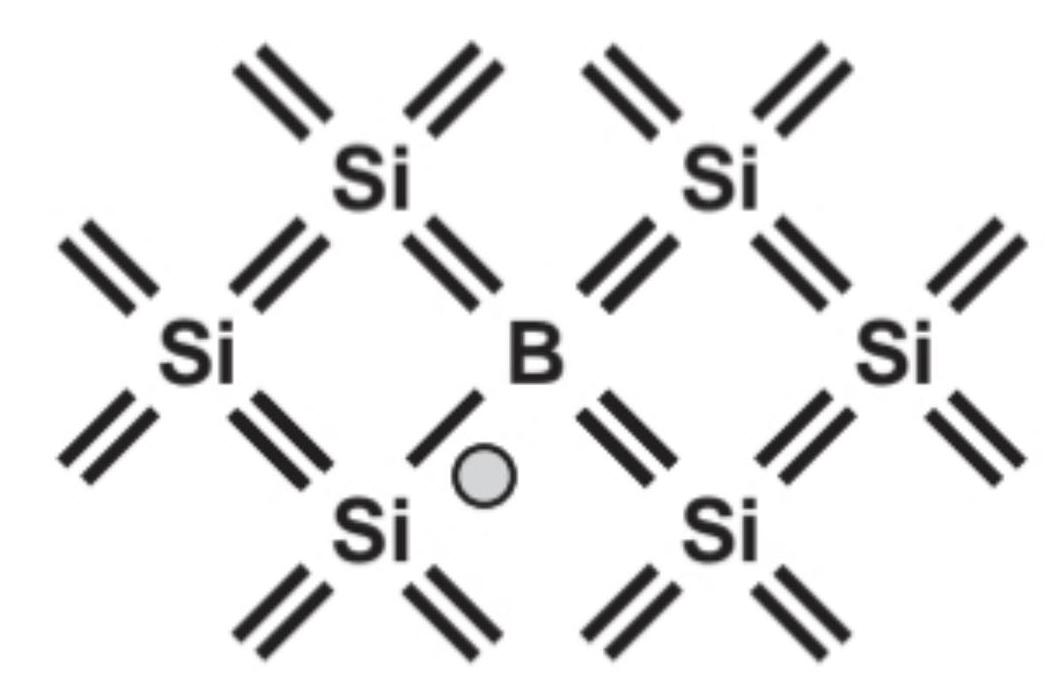
\includegraphics[max width=\textwidth, center]{2024_10_27_cec776a4495ed9df4dfcg-026}

Figure 2.6 Available hole with boron doping.

Let us formulate our results thus far. If an intrinsic semiconductor is doped with a density of $N_{D}\left(\gg n_{i}\right)$ donor atoms per cubic centimeter, then the mobile charge densities are given by


\begin{align*}
& \text { Majority Carriers: } n \approx N_{D}  \tag{2.9}\\
& \text { Minority Carriers: } p \approx \frac{n_{i}^{2}}{N_{D}} . \tag{2.10}
\end{align*}


Similarly, for a density of $N_{A}\left(\gg n_{i}\right)$ acceptor atoms per cubic centimeter:


\begin{align*}
& \text { Majority Carriers: } p \approx N_{A}  \tag{2.11}\\
& \text { Minority Carriers: } n \approx \frac{n_{i}^{2}}{N_{A}} . \tag{2.12}
\end{align*}


Since typical doping densities fall in the range of $10^{15}$ to $10^{18}$ atoms $/ \mathrm{cm}^{3}$, the above expressions are quite accurate.

\begin{center}
\begin{tabular}{|cl|}
\hline
\begin{tabular}{c}
Example \\
2.4 \\
\end{tabular} & Is it possible to use other elements of Fig. 2.2 as semiconductors and dopants? \\
\hline
Solution & \begin{tabular}{l}
Yes, for example, some early diodes and transistors were based on germanium (Ge) \\
rather than silicon. Also, arsenic (As) is another common dopant. \\
\end{tabular} \\
\hline
\end{tabular}
\end{center}

Exercise Can carbon be used for this purpose?

Figure 2.7 summarizes the concepts introduced in this section, illustrating the types of charge carriers and their densities in semiconductors.\\
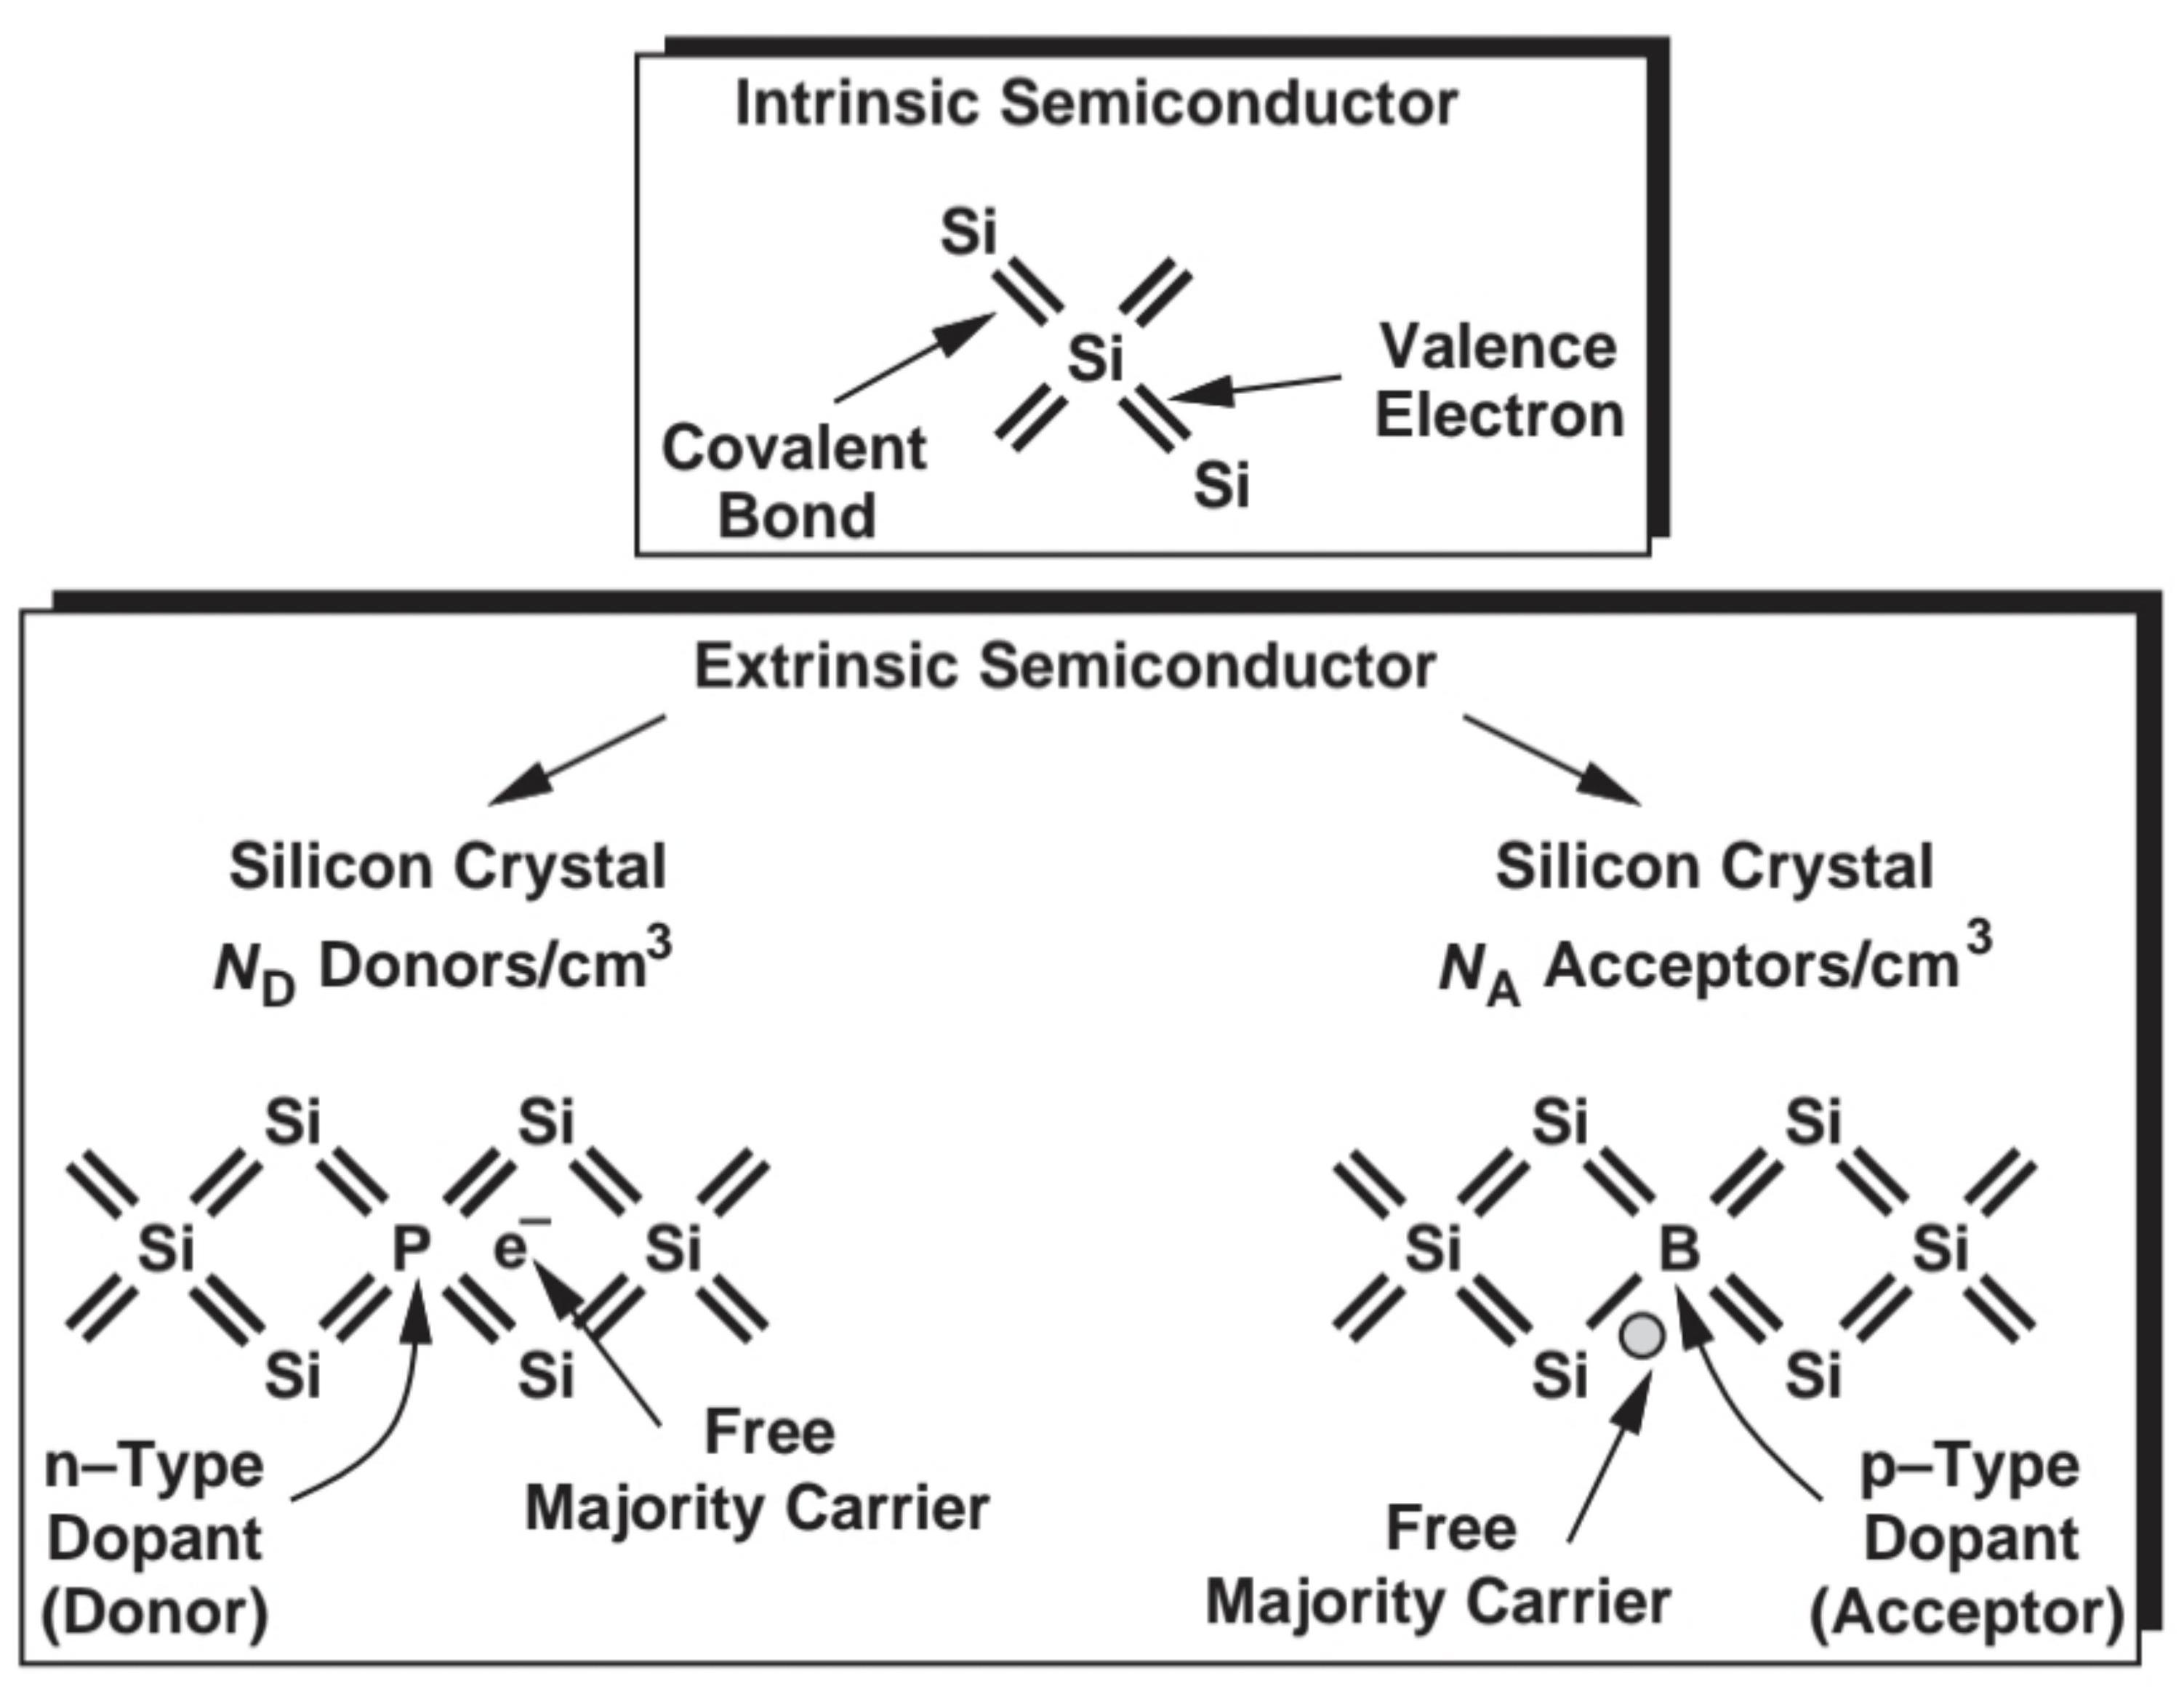
\includegraphics[max width=\textwidth, center]{2024_10_27_cec776a4495ed9df4dfcg-027}

Figure 2.7 Summary of charge carriers in silicon.

\subsection*{2.1.3 Transport of Carriers}
Having studied charge carriers and the concept of doping, we are ready to examine the movement of charge in semiconductors, i.e., the mechanisms leading to the flow of current.

Drift We know from basic physics and Ohm's law that a material can conduct current in response to a potential difference and hence an electric field. ${ }^{4}$ The field accelerates the charge carriers in the material, forcing some to flow from one end to the other. Movement of charge carriers due to an electric field is called "drift." ${ }^{5}$\\
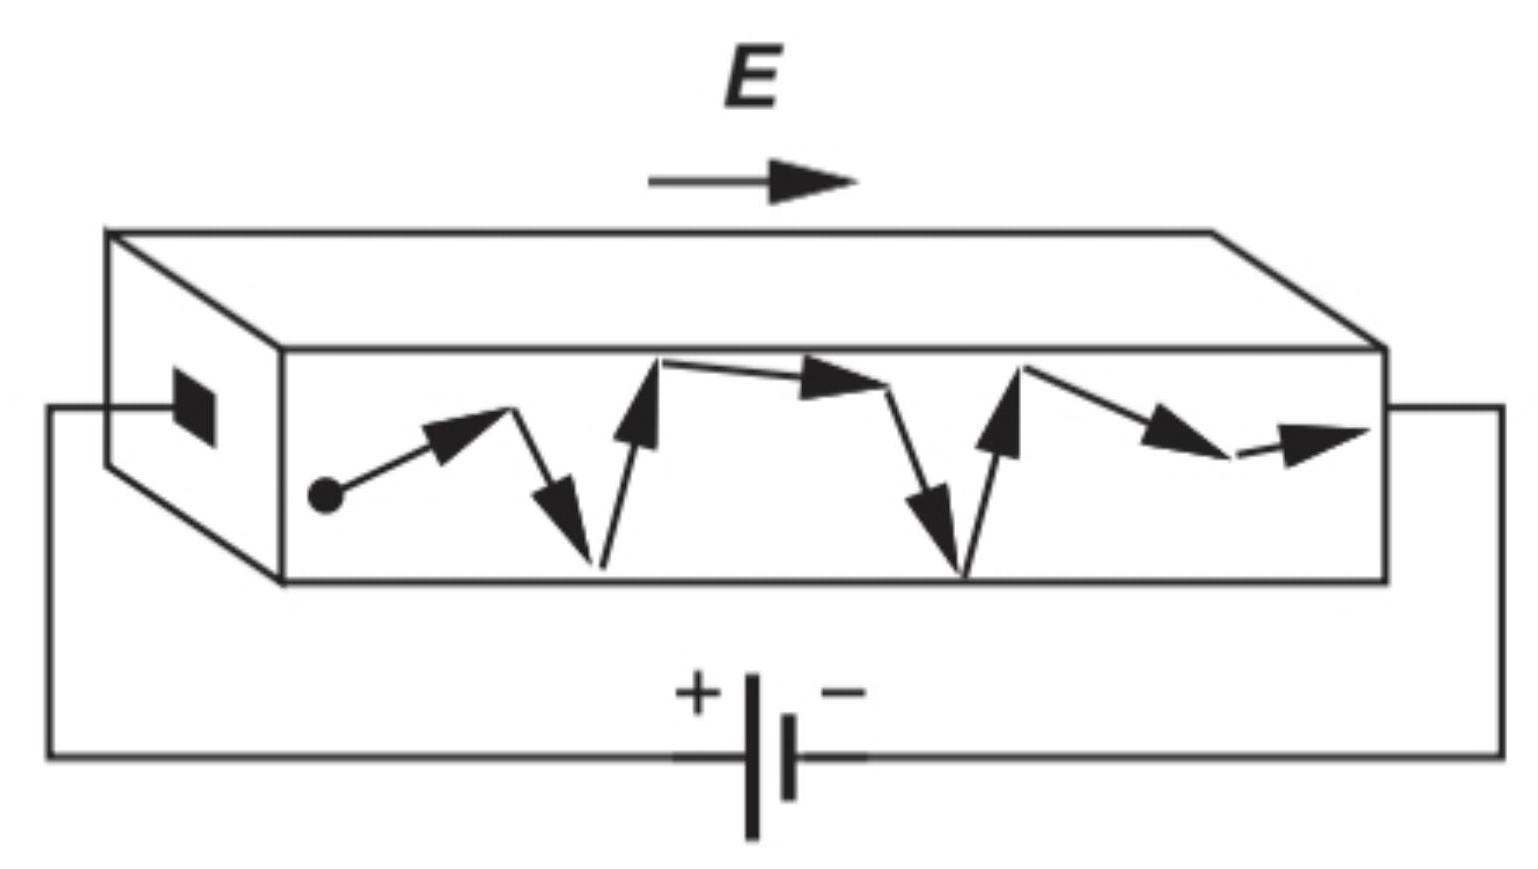
\includegraphics[max width=\textwidth, center]{2024_10_27_cec776a4495ed9df4dfcg-028}

Figure 2.8 Drift in a semiconductor.

Semiconductors behave in a similar manner. As shown in Fig. 2.8, the charge carriers are accelerated by the field and accidentally collide with the atoms in the crystal, eventually reaching the other end and flowing into the battery. The acceleration due to the field and the collision with the crystal counteract, leading to a constant velocity for the carriers. ${ }^{6} \mathrm{We}$ expect the velocity, $v$, to be proportional to the electric field strength, $E$ :


\begin{equation*}
v \propto E, \tag{2.13}
\end{equation*}


and hence


\begin{equation*}
v=\mu E \tag{2.14}
\end{equation*}


where $\mu$ is called the "mobility" and usually expressed in $\mathrm{cm}^{2} /(\mathrm{V} \cdot \mathrm{s})$. For example in silicon, the mobility of electrons, $\mu_{n}=1350 \mathrm{~cm}^{2} /(\mathrm{V} \cdot \mathrm{s})$, and that of holes, $\mu_{p}=480 \mathrm{~cm}^{2} /(\mathrm{V} \cdot \mathrm{s})$. Of course, since electrons move in a direction opposite to the electric field, we must express the velocity vector as


\begin{equation*}
\overrightarrow{v_{e}}=-\mu_{n} \vec{E} \tag{2.15}
\end{equation*}


For holes, on the other hand,


\begin{equation*}
\overrightarrow{v_{h}}=\mu_{p} \vec{E} \tag{2.16}
\end{equation*}


\footnotetext{${ }^{4}$ Recall that the potential (voltage) difference, $V$, is equal to the negative integral of the electric field, $E$, with respect to distance: $V_{a b}=-\int_{b}^{a} E d x$.\\
${ }^{5}$ The convention for direction of current assumes flow of positive charge from a positive voltage to a negative voltage. Thus, if electrons flow from point $A$ to point $B$, the current is considered to have a direction from $B$ to $A$.\\
${ }^{6}$ This phenomenon is analogous to the "terminal velocity" that a sky diver with a parachute (hopefully, open) experiences.
}\begin{center}
\begin{tabular}{|c|c|}
\hline

\includegraphics[max width=\textwidth]{2024_10_27_cec776a4495ed9df4dfcg-029}
 & A uniform piece of $n$-type of silicon that is $1 \mu \mathrm{~m}$ long senses a voltage of 1 V . Determine the velocity of the electrons. \\
\hline
Solution & Since the material is uniform, we have $E=V / L$, where $L$ is the length. Thus, $E=10,000 \mathrm{~V} / \mathrm{cm}$ and hence $v=\mu_{n} E=1.35 \times 10^{7} \mathrm{~cm} / \mathrm{s}$. In other words, electrons take $(1 \mu \mathrm{~m}) /\left(1.35 \times 10^{7} \mathrm{~cm} / \mathrm{s}\right)=7.4 \mathrm{ps}$ to cross the $1-\mu \mathrm{m}$ length. \\
\hline
\end{tabular}
\end{center}

Exercise What happens if the mobility is halved?\\
\includegraphics[max width=\textwidth, center]{2024_10_27_cec776a4495ed9df4dfcg-029(1)}

Figure 2.9 Current flow in terms of charge density.

With the velocity of carriers known, how is the current calculated? We first note that an electron carries a negative charge equal to $q=1.6 \times 10^{-19} \mathrm{C}$. Equivalently, a hole carries a positive charge of the same value. Now suppose a voltage $V_{1}$ is applied across a uniform semiconductor bar having a free electron density of $n$ (Fig. 2.9). Assuming the electrons move with a velocity of $v \mathrm{~m} / \mathrm{s}$, considering a cross section of the bar at $x=x_{1}$ and taking two "snapshots" at $t=t_{1}$ and $t=t_{1}+1$ second, we note that the total charge in $v$ meters passes the cross section in 1 second. In other words, the current is equal to the total charge enclosed in $v$ meters of the bar's length. Since the bar has a width of $W$, we have:


\begin{equation*}
I=-v \cdot W \cdot h \cdot n \cdot q \tag{2.17}
\end{equation*}


where $v \cdot W \cdot h$ represents the volume, $n \cdot q$ denotes the charge density in coulombs, and the negative sign accounts for the fact that electrons carry negative charge.

Let us now reduce Eq. (2.13) to a more convenient form. Since for electrons, $v=-\mu_{n} E$, and since $W \cdot h$ is the cross section area of the bar, we write


\begin{equation*}
J_{n}=\mu_{n} E \cdot n \cdot q, \tag{2.18}
\end{equation*}


where $J_{n}$ denotes the "current density," i.e., the current passing through a unit cross section area, and is expressed in $\mathrm{A} / \mathrm{cm}^{2}$. We may loosely say, "the current is equal to the charge velocity times the charge density," with the understanding that "current" in fact refers to current density, and negative or positive signs are taken into account properly.

In the presence of both electrons and holes, Eq. (2.18) is modified to


\begin{align*}
J_{t o t} & =\mu_{n} E \cdot n \cdot q+\mu_{p} E \cdot p \cdot q  \tag{2.19}\\
& =q\left(\mu_{n} n+\mu_{p} p\right) E . \tag{2.20}
\end{align*}


This equation gives the drift current density in response to an electric field $E$ in a semiconductor having uniform electron and hole densities.

\begin{center}
\begin{tabular}{|c|c|}
\hline
\begin{tabular}{l}
Example \\
2.6 \\
\end{tabular} & In an experiment, it is desired to obtain equal electron and hole drift currents. How should the carrier densities be chosen? \\
\hline
\multirow[t]{11}{*}{Solution} & We must impose \\
\hline
 & $\mu_{n} n=\mu_{p} p$, \\
\hline
 & and hence \\
\hline
 & \( \begin{equation*} \frac{n}{p}=\frac{\mu_{p}}{\mu_{n}} . \tag{2.22} \end{equation*} \) \\
\hline
 & We also recall that $n p=n_{i}^{2}$. Thus, \\
\hline
 & $p=\sqrt{\frac{\mu_{n}}{\mu_{p}}} n_{i}$ \\
\hline
 & $n=\sqrt{\frac{\mu_{p}}{\mu_{n}}} n_{i}$ \\
\hline
 & For example, in silicon, $\mu_{n} / \mu_{p}=1350 / 480=2.81$, yielding \\
\hline
 & $p=1.68 n_{i}$ \\
\hline
 & $n=0.596 n_{i} . \quad(2.26)$ \\
\hline
 & Since $p$ and $n$ are of the same order as $n_{i}$, equal electron and hole drift currents can occur for only a very lightly doped material. This confirms our earlier notion of majority carriers in semiconductors having typical doping levels of $10^{15}-10^{18}$ atoms $/ \mathrm{cm}^{3}$. \\
\hline
\end{tabular}
\end{center}

Exercise How should the carrier densities be chosen so that the electron drift current is twice the hole drift current?

Velocity Saturation* We have thus far assumed that the mobility of carriers in semiconductors is independent of the electric field and the velocity rises linearly with $E$ according to $v=\mu E$. In reality, if the electric field approaches sufficiently high levels, $v$ no longer follows $E$ linearly. This is because the carriers collide with the lattice so frequently and the time between the collisions is so short that they cannot accelerate much. As a result, $v$ varies "sublinearly" at high electric fields, eventually reaching a saturated level, $v_{s a t}$ (Fig. 2.10). Called "velocity saturation," this effect manifests itself in some modern transistors, limiting the performance of circuits.

In order to represent velocity saturation, we must modify $v=\mu E$ accordingly. A simple approach is to view the slope, $\mu$, as a field-dependent parameter. The expression

\footnotetext{*This section can be skipped in a first reading.
}
\includegraphics[max width=\textwidth, center]{2024_10_27_cec776a4495ed9df4dfcg-031(1)}

Figure 2.10 Velocity saturation.\\
for $\mu$ must therefore gradually fall toward zero as $E$ rises, but approach a constant value for small $E$; i.e.,


\begin{equation*}
\mu=\frac{\mu_{0}}{1+b E} \tag{2.27}
\end{equation*}


where $\mu_{0}$ is the "low-field" mobility and $b$ a proportionality factor. We may consider $\mu$ as the "effective" mobility at an electric field $E$. Thus,


\begin{equation*}
v=\frac{\mu_{0}}{1+b E} E \tag{2.28}
\end{equation*}


Since for $E \rightarrow \infty, v \rightarrow v_{\text {sat }}$, we have


\begin{equation*}
v_{s a t}=\frac{\mu_{0}}{b} \tag{2.29}
\end{equation*}


and hence $b=\mu_{0} / v_{\text {sat }}$. In other words,


\begin{equation*}
v=\frac{\mu_{0}}{1+\frac{\mu_{0} E}{v_{s a t}}} E \tag{2.30}
\end{equation*}


\begin{center}
\includegraphics[max width=\textwidth]{2024_10_27_cec776a4495ed9df4dfcg-031}
\end{center}

A uniform piece of semiconductor $0.2 \mu \mathrm{~m}$ long sustains a voltage of 1 V . If the low-field mobility is equal to $1350 \mathrm{~cm}^{2} /(\mathrm{V} \cdot \mathrm{s})$ and the saturation velocity of the carriers $10^{7} \mathrm{~cm} / \mathrm{s}$, determine the effective mobility. Also, calculate the maximum allowable voltage such that the effective mobility is only $10 \%$ lower than $\mu_{0}$.

Solution We have


\begin{align*}
E & =\frac{V}{L}  \tag{2.31}\\
& =50 \mathrm{kV} / \mathrm{cm} \tag{2.32}
\end{align*}


It follows that


\begin{align*}
\mu & =\frac{\mu_{0}}{1+\frac{\mu_{0} E}{v_{s a t}}}  \tag{2.33}\\
& =\frac{\mu_{0}}{7.75}  \tag{2.34}\\
& =174 \mathrm{~cm}^{2} /(\mathrm{V} \cdot \mathrm{~s}) \tag{2.35}
\end{align*}


If the mobility must remain within $10 \%$ of its low-field value, then


\begin{equation*}
0.9 \mu_{0}=\frac{\mu_{0}}{1+\frac{\mu_{0} E}{v_{s a t}}} \tag{2.36}
\end{equation*}


and hence


\begin{align*}
E & =\frac{1}{9} \frac{v_{\text {sat }}}{\mu_{0}}  \tag{2.37}\\
& =823 \mathrm{~V} / \mathrm{cm} \tag{2.38}
\end{align*}


A device of length $0.2 \mu \mathrm{~m}$ experiences such a field if it sustains a voltage of $(823 \mathrm{~V} / \mathrm{cm}) \times\left(0.2 \times 10^{-4} \mathrm{~cm}\right)=16.5 \mathrm{mV}$.

This example suggests that modern (submicron) devices incur substantial velocity saturation because they operate with voltages much greater than 16.5 mV .

Exercise At what voltage does the mobility fall by 20\%?

Diffusion In addition to drift, another mechanism can lead to current flow. Suppose a drop of ink falls into a glass of water. Introducing a high local concentration of ink molecules, the drop begins to "diffuse," that is, the ink molecules tend to flow from a region of high concentration to regions of low concentration. This mechanism is called "diffusion."

A similar phenomenon occurs if charge carriers are "dropped" (injected) into a semiconductor so as to create a nonuniform density. Even in the absence of an electric field, the carriers move toward regions of low concentration, thereby carrying an electric current so long as the nonuniformity is sustained. Diffusion is therefore distinctly different from drift.\\
\includegraphics[max width=\textwidth, center]{2024_10_27_cec776a4495ed9df4dfcg-032}

Figure 2.11 Diffusion in a semiconductor.

Figure 2.11 conceptually illustrates the process of diffusion. A source on the left continues to inject charge carriers into the semiconductor, a nonuniform charge profile is created along the $x$-axis, and the carriers continue to "roll down" the profile.

The reader may raise several questions at this point. What serves as the source of carriers in Fig. 2.11? Where do the charge carriers go after they roll down to the end of the profile at the far right? And, most importantly, why should we care?! Well, patience is a virtue and we will answer these questions in the next section.

Example 2.8

A source injects charge carriers into a semiconductor bar as shown in Fig. 2.12. Explain how the current flows.\\
\includegraphics[max width=\textwidth, center]{2024_10_27_cec776a4495ed9df4dfcg-033}

Figure 2.12 Injection of carriers into a semiconductor.\\
Solution In this case, two symmetric profiles may develop in both positive and negative directions along the $x$-axis, leading to current flow from the source toward the two ends of the bar.

Exercise Is KCL still satisfied at the point of injection?

Our qualitative study of diffusion suggests that the more nonuniform the concentration, the larger the current. More specifically, we can write:


\begin{equation*}
I \propto \frac{d n}{d x} \tag{2.39}
\end{equation*}


where $n$ denotes the carrier concentration at a given point along the $x$-axis. We call $d n / d x$ the concentration "gradient" with respect to $x$, assuming current flow only in the $x$ direction. If each carrier has a charge equal to $q$, and the semiconductor has a cross section area of $A$, Eq. (2.39) can be written as


\begin{equation*}
I \propto A q \frac{d n}{d x} \tag{2.40}
\end{equation*}


Thus,


\begin{equation*}
I=A q D_{n} \frac{d n}{d x} \tag{2.41}
\end{equation*}


where $D_{n}$ is a proportionality factor called the "diffusion constant" and expressed in $\mathrm{cm}^{2} / \mathrm{s}$. For example, in intrinsic silicon, $D_{n}=34 \mathrm{~cm}^{2} / \mathrm{s}$ (for electrons), and $D_{p}=12 \mathrm{~cm}^{2} / \mathrm{s}$ (for holes).

As with the convention used for the drift current, we normalize the diffusion current to the cross section area, obtaining the current density as


\begin{equation*}
J_{n}=q D_{n} \frac{d n}{d x} \tag{2.42}
\end{equation*}


Similarly, a gradient in hole concentration yields:


\begin{equation*}
J_{p}=-q D_{p} \frac{d p}{d x} \tag{2.43}
\end{equation*}


With both electron and hole concentration gradients present, the total current density is given by


\begin{equation*}
J_{t o t}=q\left(D_{n} \frac{d n}{d x}-D_{p} \frac{d p}{d x}\right) \tag{2.44}
\end{equation*}


Example Consider the scenario depicted in Fig. 2.11 again. Suppose the electron concentration is\\
equal to $N$ at $x=0$ and falls linearly to zero at $x=L$ (Fig. 2.13). Determine the diffusion current.\\
\includegraphics[max width=\textwidth, center]{2024_10_27_cec776a4495ed9df4dfcg-034}

Figure 2.13 Current resulting from a linear diffusion profile.

Solution We have


\begin{align*}
J_{n} & =q D_{n} \frac{d n}{d x}  \tag{2.45}\\
& =-q D_{n} \cdot \frac{N}{I} \tag{2.46}
\end{align*}


The current is constant along the $x$-axis; i.e., all of the electrons entering the material at $x=0$ successfully reach the point at $x=L$. While obvious, this observation prepares us for the next example.

Exercise Repeat the above example for holes.

Example Repeat the above example but assume an exponential gradient (Fig. 2.14):\\
2.10\\
\includegraphics[max width=\textwidth, center]{2024_10_27_cec776a4495ed9df4dfcg-034(1)}

Figure 2.14 Current resulting from an exponential diffusion profile.


\begin{equation*}
n(x)=N \exp \frac{-x}{L_{d}} \tag{2.47}
\end{equation*}


where $L_{d}$ is a constant. ${ }^{7}$

\footnotetext{${ }^{7}$ The factor $L_{d}$ is necessary to convert the exponent to a dimensionless quantity.
}Solution We have


\begin{align*}
J_{n} & =q D_{n} \frac{d n}{d x}  \tag{2.48}\\
& =\frac{-q D_{n} N}{L_{d}} \exp \frac{-x}{L_{d}} . \tag{2.49}
\end{align*}


Interestingly, the current is not constant along the $x$-axis. That is, some electrons vanish while traveling from $x=0$ to the right. What happens to these electrons? Does this example violate the law of conservation of charge? These are important questions and will be answered in the next section.

Exercise At what value of $x$ does the current density drop to $1 \%$ of its maximum value?

Einstein Relation Our study of drift and diffusion has introduced a factor for each: $\mu_{n}$ (or $\mu_{p}$ ) and $D_{n}$ (or $D_{p}$ ), respectively. It can be proved that $\mu$ and $D$ are related as:


\begin{equation*}
\frac{D}{\mu}=\frac{k T}{q} \tag{2.50}
\end{equation*}


Called the "Einstein Relation," this result is proved in semiconductor physics texts, e.g., [1]. Note that $k T / q \approx 26 \mathrm{mV}$ at $T=300 \mathrm{~K}$.

Figure 2.15 summarizes the charge transport mechanisms studied in this section.\\
\includegraphics[max width=\textwidth, center]{2024_10_27_cec776a4495ed9df4dfcg-035}

Figure 2.15 Summary of drift and diffusion mechanisms.

\section*{2.2 pn JUNCTION}
We begin our study of semiconductor devices with the $p n$ junction for three reasons. (1) The device finds application in many electronic systems, e.g., in adaptors that charge the batteries of cellphones. (2) The $p n$ junction is among the simplest semiconductor devices, thus providing a good entry point into the study of the operation of such complex structures as transistors.

\section*{Did you know?}
The pn junction was inadvertantly invented by Russel Ohl of Bell Laboratories in 1940. He melted silicon in quartz tubes to achieve a high purity. During the cooling process, the $p$-type and $n$-type impurities redistributed themselves, creating a pn junction. Ohl even observed that the pn junction produced a current when it was exposed to light. One wonders if Ohl ever predicted that this property would eventually lead to the invention of the digital camera.\\
(3) The $p n$ junction also serves as part of transistors. We also use the term "diode" to refer to $p n$ junctions.

We have thus far seen that doping produces free electrons or holes in a semiconductor, and an electric field or a concentration gradient leads to the movement of these charge carriers. An interesting situation arises if we introduce $n$-type and $p$-type dopants into two adjacent sections of a piece of semiconductor. Depicted in Fig. 2.16 and called a " $p n$ junction," this structure plays a fundamental role in many semiconductor devices. The $p$ and $n$ sides are called the "anode" and the "cathode," respectively.\\
\includegraphics[max width=\textwidth, center]{2024_10_27_cec776a4495ed9df4dfcg-036(1)}

Figure 2.16 pn junction.

In this section, we study the properties and I/V characteristics of pn junctions. The following outline shows our thought process, indicating that our objective is to develop circuit models that can be used in analysis and design.\\
\includegraphics[max width=\textwidth, center]{2024_10_27_cec776a4495ed9df4dfcg-036}

Figure 2.17 Outline of concepts to be studied.

\subsection*{2.2.1 pn Junction in Equilibrium}
Let us first study the pn junction with no external connections, i.e., the terminals are open and no voltage is applied across the device. We say the junction is in "equilibrium." While seemingly of no practical value, this condition provides insights that prove useful in understanding the operation under nonequilibrium as well.

We begin by examining the interface between the $n$ and $p$ sections, recognizing that one side contains a large excess of holes and the other, a large excess of electrons. The sharp concentration gradient for both electrons and holes across the junction leads to two large diffusion currents: electrons flow from the $n$ side to the $p$ side, and holes flow in the opposite direction. Since we must deal with both electron and hole concentrations on each side of the junction, we introduce the notations shown in Fig. 2.18.\\
\includegraphics[max width=\textwidth, center]{2024_10_27_cec776a4495ed9df4dfcg-037}

Figure 2.18

Example A $p n$ junction employs the following doping levels: $N_{A}=10^{16} \mathrm{~cm}^{-3}$ and $N_{D}=$ $2.115 \times 10^{15} \mathrm{~cm}^{-3}$. Determine the hole and electron concentrations on the two sides.

Solution From Eqs. (2.11) and (2.12), we express the concentrations of holes and electrons on the $p$ side respectively as:


\begin{align*}
p_{p} & \approx N_{A}  \tag{2.51}\\
& =10^{16} \mathrm{~cm}^{-3}  \tag{2.52}\\
n_{p} & \approx \frac{n_{i}^{2}}{N_{A}}  \tag{2.53}\\
& =\frac{\left(1.08 \times 10^{10} \mathrm{~cm}^{-3}\right)^{2}}{10^{16} \mathrm{~cm}^{-3}}  \tag{2.54}\\
& \approx 1.1 \times 10^{4} \mathrm{~cm}^{-3} \tag{2.55}
\end{align*}


Similarly, the concentrations on the $n$ side are given by


\begin{align*}
n_{n} & \approx N_{D}  \tag{2.56}\\
& =5 \times 10^{15} \mathrm{~cm}^{-3}  \tag{2.57}\\
p_{n} & \approx \frac{n_{i}^{2}}{N_{D}}  \tag{2.58}\\
& =\frac{\left(1.08 \times 10^{10} \mathrm{~cm}^{-3}\right)^{2}}{5 \times 10^{15} \mathrm{~cm}^{-3}}  \tag{2.59}\\
& =2.3 \times 10^{4} \mathrm{~cm}^{-3} \tag{2.60}
\end{align*}


Note that the majority carrier concentration on each side is many orders of magnitude higher than the minority carrier concentration on either side.

Exercise Repeat the above example if $N_{D}$ drops by a factor of four.

\section*{test}
\begin{center}
\includegraphics[max width=\textwidth]{2024_10_27_cec776a4495ed9df4dfcg-038(1)}
\end{center}

The diffusion currents transport a great deal of charge from each side to the other, but they must eventually decay to zero. This is because if the terminals are left open (equilibrium condition), the device cannot carry a net current indefinitely.

We must now answer an important question: what stops the diffusion currents? We may postulate that the currents stop after enough free carriers have moved across the junction so as to equalize the concentrations on the two sides. However, another effect dominates the situation and stops the diffusion currents well before this point is reached.

To understand this effect, we recognize that for every electron that departs from the $n$ side, a positive ion is left behind, i.e., the junction evolves with time as conceptually shown in Fig. 2.19. In this illustration, the junction is suddenly formed at $t=0$, and the diffusion currents continue to expose more ions as time progresses. Consequently, the immediate vicinity of the junction is depleted of free carriers and hence called the "depletion region."\\
\includegraphics[max width=\textwidth, center]{2024_10_27_cec776a4495ed9df4dfcg-038(2)}

Figure 2.19 Evolution of charge concentrations in a pn junction.\\
Now recall from basic physics that a particle or object carrying a net (nonzero) charge creates an electric field around it. Thus, with the formation of the depletion region, an electric field emerges as shown in Fig. 2.20. ${ }^{8}$ Interestingly, the field tends to force positive charge flow from left to right whereas the concentration gradients necessitate the flow of holes from right to left (and electrons from left to right). We therefore surmise that the junction reaches equilibrium once the electric field is strong enough to completely stop the diffusion currents. Alternatively, we can say, in equilibrium, the drift currents resulting from the electric field exactly cancel the diffusion currents due to the gradients.\\
\includegraphics[max width=\textwidth, center]{2024_10_27_cec776a4495ed9df4dfcg-038}

Figure 2.20 Electric field in a pn junction.

\footnotetext{${ }^{8}$ The direction of the electric field is determined by placing a small positive test charge in the region and watching how it moves: away from positive charge and toward negative charge.
}Example\\
2.12

In the junction shown in Fig. 2.21, the depletion region has a width of $b$ on the $n$ side and $a$ on the $p$ side. Sketch the electric field as a function of $x$.\\
\includegraphics[max width=\textwidth, center]{2024_10_27_cec776a4495ed9df4dfcg-039}

Figure 2.21 Electric field profile in a $p n$ junction.

Solution Beginning at $x<-b$, we note that the absence of net charge yields $E=0$. At $x>-b$, each positive donor ion contributes to the electric field, i.e., the magnitude of $E$ rises as $x$ approaches zero. As we pass $x=0$, the negative acceptor atoms begin to contribute negatively to the field, i.e., $E$ falls. At $x=a$, the negative and positive charge exactly cancel each other and $E=0$.

Exercise Noting that potential voltage is negative integral of electric field with respect to distance, plot the potential as a function of $x$.

From our observation regarding the drift and diffusion currents under equilibrium, we may be tempted to write:


\begin{equation*}
\left|I_{\mathrm{drift}, p}+I_{\mathrm{drift}, n}\right|=\left|I_{\mathrm{diff}, p}+I_{\mathrm{diff}, n}\right|, \tag{2.61}
\end{equation*}


where the subscripts $p$ and $n$ refer to holes and electrons, respectively, and each current term contains the proper polarity. This condition, however, allows an unrealistic phenomenon: if the number of the electrons flowing from the $n$ side to the $p$ side is equal to that of the holes going from the $p$ side to the $n$ side, then each side of this equation is zero while electrons continue to accumulate on the $p$ side and holes on the $n$ side. We must therefore impose the equilibrium condition on each carrier:


\begin{align*}
& \left|I_{\mathrm{drift}, p}\right|=\left|I_{\mathrm{diff}, p}\right|  \tag{2.62}\\
& \left|I_{\mathrm{drift}, n}\right|=\left|I_{\mathrm{diff}, n}\right| \tag{2.63}
\end{align*}


Built-in Potential The existence of an electric field within the depletion region suggests that the junction may exhibit a "built-in potential." In fact, using (2.62) or (2.63), we can compute this potential. Since the electric field $E=-d V / d x$, and since (2.62) can be written as


\begin{equation*}
q \mu_{p} p E=q D_{p} \frac{d p}{d x} \tag{2.64}
\end{equation*}


we have


\begin{equation*}
-\mu_{p} p \frac{d V}{d x}=D_{p} \frac{d p}{d x} \tag{2.65}
\end{equation*}


Dividing both sides by $p$ and taking the integral, we obtain


\begin{equation*}
-\mu_{p} \int_{x_{1}}^{x_{2}} d V=D_{p} \int_{p_{n}}^{p_{p}} \frac{d p}{p} \tag{2.66}
\end{equation*}


where $p_{n}$ and $p_{p}$ are the hole concentrations at $x_{1}$ and $x_{2}$, respectively (Fig. 2.22). Thus,


\begin{equation*}
V\left(x_{2}\right)-V\left(x_{1}\right)=-\frac{D_{p}}{\mu_{p}} \ln \frac{p_{p}}{p_{n}} \tag{2.67}
\end{equation*}


\begin{center}
\includegraphics[max width=\textwidth]{2024_10_27_cec776a4495ed9df4dfcg-040}
\end{center}

Figure 2.22 Carrier profiles in a pn junction.\\
The right side represents the voltage difference developed across the depletion region and will be denoted by $V_{0}$. Also, from Einstein's relation, Eq. (2.50), we can replace $D_{p} / \mu_{p}$ with $k T / q$ :


\begin{equation*}
\left|V_{0}\right|=\frac{k T}{q} \ln \frac{p_{p}}{p_{n}} . \tag{2.68}
\end{equation*}


Exercise Writing Eq. (2.64) for electron drift and diffusion currents, and carrying out the integration, derive an equation for $V_{0}$ in terms of $n_{n}$ and $n_{p}$.

Finally, using (2.11) and (2.10) for $p_{p}$ and $p_{n}$ yields


\begin{equation*}
V_{0}=\frac{k T}{q} \ln \frac{N_{A} N_{D}}{n_{i}^{2}} \tag{2.69}
\end{equation*}


Expressing the built-in potential in terms of junction parameters, this equation plays a central role in many semiconductor devices.

\begin{center}
\begin{tabular}{|c|c|c|}
\hline
Example \( 2.13 \) & \multicolumn{2}{|l|}{A silicon $p n$ junction employs $N_{A}=2 \times 10^{16} \mathrm{~cm}^{-3}$ and $N_{D}=4 \times 10^{16} \mathrm{~cm}^{-3}$. Determine the built-in potential at room temperature ( $T=300 \mathrm{~K}$ ).} \\
\hline
\multirow[t]{2}{*}{Solution} & Recall from Example 2.1 that $n_{i}(T=300 \mathrm{~K})=1.08 \times 10^{10} \mathrm{~cm}^{-3}$. Thus, \( V_{0} \approx(26 \mathrm{mV}) \ln \frac{\left(2 \times 10^{16}\right) \times\left(4 \times 10^{16}\right)}{\left(1.08 \times 10^{10}\right)^{2}} \) & (2.70) \\
\hline
 & $\approx 768 \mathrm{mV}$. & (2.71) \\
\hline
\end{tabular}
\end{center}

Exercise By what factor should $N_{D}$ be changed to lower $V_{0}$ by 20 mV ?

\section*{test}
\begin{center}
\includegraphics[max width=\textwidth]{2024_10_27_cec776a4495ed9df4dfcg-041}
\end{center}

\begin{center}
\begin{tabular}{|c|c|c|c|}
\hline
\begin{tabular}{l}
Example \\
2.14 \\
\end{tabular} & \multicolumn{3}{|l|}{Equation (2.69) reveals that $V_{0}$ is a weak function of the doping levels. How much does $V_{0}$ change if $N_{A}$ or $N_{D}$ is increased by one order of magnitude?} \\
\hline
\multirow[t]{4}{*}{Solution} & We can write &  &  \\
\hline
 &  & \( \Delta V_{0}=V_{T} \ln \frac{10 N_{A} \cdot N_{D}}{n_{i}^{2}}-V_{T} \ln \frac{N_{A} \cdot N_{D}}{n_{i}^{2}} \) & $(2.72)$ \\
\hline
 &  & $=V_{T} \ln 10$ & $(2.73)$ \\
\hline
 &  & $\approx 60 \mathrm{mV}($ at $T=300 \mathrm{~K})$. & (2.74) \\
\hline
\end{tabular}
\end{center}

Exercise How much does $V_{0}$ change if $N_{A}$ or $N_{D}$ is increased by a factor of three?

An interesting question may arise at this point. The junction carries no net current (because its terminals remain open), but it sustains a voltage. How is that possible? We observe that the built-in potential is developed to oppose the flow of diffusion currents (and is, in fact, sometimes called the "potential barrier"). This phenomenon is in contrast to the behavior of a uniform conducting material, which exhibits no tendency for diffusion and hence no need to create a built-in voltage.

\subsection*{2.2.2 pn Junction Under Reverse Bias}
Having analyzed the $p n$ junction in equilibrium, we can now study its behavior under more interesting and useful conditions. Let us begin by applying an external voltage across the device as shown in Fig. 2.23, where the voltage source makes the $n$ side more positive than the $p$ side. We say the junction is under "reverse bias" to emphasize the connection of the positive voltage to the $n$ terminal. Used as a noun or a verb, the term "bias" indicates operation under some "desirable" conditions. We will study the concept of biasing extensively in this and following chapters.\\
\includegraphics[max width=\textwidth, center]{2024_10_27_cec776a4495ed9df4dfcg-041(1)}

Figure $2.23 p n$ junction under reverse bias.

\section*{test}
\includegraphics[max width=\textwidth, center]{2024_10_27_cec776a4495ed9df4dfcg-042}\\
\includegraphics[max width=\textwidth, center]{2024_10_27_cec776a4495ed9df4dfcg-042(1)}

Figure 2.24 Reduction of junction capacitance with reverse bias.

We wish to reexamine the results obtained in equilibrium for the case of reverse bias. Let us first determine whether the external voltage enhances the built-in electric field or opposes it. Since under equilibrium, $\vec{E}$ is directed from the $n$ side to the $p$ side, $V_{R}$ enhances the field. But, a higher electric field can be sustained only if a larger amount of fixed charge is provided, requiring that more acceptor and donor ions be exposed and, therefore, the depletion region be widened.

What happens to the diffusion and drift currents? Since the external voltage has strengthened the field, the barrier rises even higher than that in equilibrium, thus prohibiting the flow of current. In other words, the junction carries a negligible current under reverse bias. ${ }^{9}$

With no current conduction, a reverse-biased pn junction does not seem particularly useful. However, an important observation will prove otherwise. We note that in Fig. 2.23, as $V_{B}$ increases, more positive charge appears on the $n$ side and more negative charge on the $p$ side. Thus, the device operates as a capacitor [Fig. 2.24(a)]. In essence, we can view the conductive $n$ and $p$ sections as the two plates of the capacitor. We also assume the charge in the depletion region equivalently resides on each plate.

The reader may still not find the device interesting. After all, since any two parallel plates can form a capacitor, the use of a $p n$ junction for this purpose is not justified. But, reverse-biased $p n$ junctions exhibit a unique property that becomes useful in circuit design. Returning to Fig. 2.23, we recognize that, as $V_{R}$ increases, so does the width of the depletion region. That is, the conceptual diagram of Fig. 2.24(a) can be drawn as in Fig. 2.24(b) for increasing values of $V_{R}$, revealing that the capacitance of the structure decreases as the two plates move away from each other. The junction therefore displays a voltage-dependent capacitance.

It can be proved that the capacitance of the junction per unit area is equal to


\begin{equation*}
C_{j}=\frac{C_{j 0}}{\sqrt{1-\frac{V_{R}}{V_{0}}}}, \tag{2.75}
\end{equation*}


\footnotetext{${ }^{9}$ As explained in Section 2.2.3, the current is not exactly zero.
}
where $C_{j 0}$ denotes the capacitance corresponding to zero bias $\left(V_{R}=0\right)$ and $V_{0}$ is the builtin potential [Eq. (2.69)]. (This equation assumes $V_{R}$ is negative for reverse bias.) The value of $C_{j 0}$ is in turn given by\\
\$\$

\begin{equation*}
C_{j 0}=\sqrt{\frac{\epsilon_{s i} q}{2} \frac{N_{A} N_{D}}{N_{A}+N_{D}} \frac{1}{V_{0}}} \tag{2.76}
\end{equation*}

\$\$\\
where $\epsilon_{s i}$ represents the dielectric constant of silicon and is equal to $11.7 \times$ $8.85 \times 10^{-14} \mathrm{~F} / \mathrm{cm} .{ }^{10}$ Plotted in Fig. 2.25, $C_{j}$ indeed decreases as $V_{R}$ increases.\\
\includegraphics[max width=\textwidth, center]{2024_10_27_cec776a4495ed9df4dfcg-043}

Figure 2.25 Junction capacitance under reverse bias.

A $p n$ junction is doped with $N_{A}=2 \times 10^{16} \mathrm{~cm}^{-3}$ and $N_{D}=9 \times 10^{15} \mathrm{~cm}^{-3}$. Determine the capacitance of the device with (a) $V_{R}=0$ and $V_{R}=1 \mathrm{~V}$.

Solution We first obtain the built-in potential:


\begin{align*}
V_{0} & =V_{T} \ln \frac{N_{A} N_{D}}{n_{i}^{2}}  \tag{2.77}\\
& =0.73 \mathrm{~V} \tag{2.78}
\end{align*}


Thus, for $V_{R}=0$ and $q=1.6 \times 10^{-19} \mathrm{C}$, we have


\begin{align*}
C_{j 0} & =\sqrt{\frac{\epsilon_{s i} q}{2} \frac{N_{A} N_{D}}{N_{A}+N_{D}} \cdot \frac{1}{V_{0}}}  \tag{2.79}\\
& =2.65 \times 10^{-8} \mathrm{~F} / \mathrm{cm}^{2} \tag{2.80}
\end{align*}


In microelectronics, we deal with very small devices and may rewrite this result as


\begin{equation*}
C_{j 0}=0.265 \mathrm{fF} / \mu \mathrm{m}^{2} \tag{2.81}
\end{equation*}


${ }^{10}$ The dielectric constant of materials is usually written in the form $\epsilon_{r} \epsilon_{0}$, where $\epsilon_{r}$ is the "relative" dielectric constant and a dimensionless factor (e.g., 11.7), and $\epsilon_{0}$ the dielectric constant of vacuum $\left(8.85 \times 10^{-14} \mathrm{~F} / \mathrm{cm}\right)$.

44 Chapter 2 Basic Physics of Semiconductors\\
where $1 \mathrm{fF}($ femtofarad $)=10^{-15} \mathrm{~F}$. For $V_{R}=1 \mathrm{~V}$,


\begin{align*}
C_{j} & =\frac{C_{j 0}}{\sqrt{1+\frac{V_{R}}{V_{0}}}}  \tag{2.82}\\
& =0.172 \mathrm{fF} / \mu \mathrm{m}^{2} \tag{2.83}
\end{align*}


Exercise Repeat the above example if the donor concentration on the $N$ side is doubled. Compare the results in the two cases.

The variation of the capacitance with the applied voltage makes the device a "nonlinear" capacitor because it does not satisfy $Q=C V$. Nonetheless, as demonstrated by the following example, a voltage-dependent capacitor leads to interesting circuit topologies.

A cellphone incorporates a 2-GHz oscillator whose frequency is defined by the resonance 2.16 frequency of an $L C \operatorname{tank}$ (Fig. 2.26). If the tank capacitance is realized as the $p n$ junction of Example 2.15, calculate the change in the oscillation frequency while the reverse voltage goes from 0 to 2 V . Assume the circuit operates at 2 GHz at a reverse voltage of 0 V , and the junction area is $2000 ~ \mu \mathrm{~m}^{2}$.\\
\includegraphics[max width=\textwidth, center]{2024_10_27_cec776a4495ed9df4dfcg-044}

Figure 2.26 Variable capacitor used to tune an oscillator.

Solution Recall from basic circuit theory that the tank "resonates" if the impedances of the inductor and the capacitor are equal and opposite: $j L \omega_{\text {res }}=-\left(j C \omega_{\text {res }}\right)^{-1}$. Thus, the resonance frequency is equal to


\begin{equation*}
f_{r e s}=\frac{1}{2 \pi} \frac{1}{\sqrt{L C}} \tag{2.84}
\end{equation*}


At $V_{R}=0, C_{j}=0.265 \mathrm{fF} / \mu \mathrm{m}^{2}$, yielding a total device capacitance of


\begin{align*}
C_{j, t o t}\left(V_{R}=0\right) & =\left(0.265 \mathrm{fF} / \mu \mathrm{m}^{2}\right) \times\left(2000 \mu \mathrm{~m}^{2}\right)  \tag{2.85}\\
& =530 \mathrm{fF} \tag{2.86}
\end{align*}


Setting $f_{\text {res }}$ to 2 GHz , we obtain


\begin{equation*}
L=11.9 \mathrm{nH} \tag{2.87}
\end{equation*}


$V_{R}$ goes to 2 V ,


\begin{align*}
C_{j, t o t}\left(V_{R}=2 \mathrm{~V}\right) & =\frac{C_{j 0}}{\sqrt{1+\frac{2}{0.73}}} \times 2000 \mu \mathrm{~m}^{2}  \tag{2.88}\\
& =274 \mathrm{fF} \tag{2.89}
\end{align*}


Using this value along with $L=11.9 \mathrm{nH}$ in Eq. (2.84), we have


\begin{equation*}
f_{r e s}\left(V_{R}=2 \mathrm{~V}\right)=2.79 \mathrm{GHz} \tag{2.90}
\end{equation*}


An oscillator whose frequency can be varied by an external voltage ( $V_{R}$ in this case) is called a "voltage-controlled oscillator" and used extensively in cellphones, microprocessors, personal computers, etc.

Exercise Some wireless systems operate at 5.2 GHz . Repeat the above example for this frequency, assuming the junction area is still $2000 ~ \mu \mathrm{~m}^{2}$ but the inductor value is scaled to reach 5.2 GHz .

In summary, a reverse-biased pn junction carries a negligible current but exhibits a voltage-dependent capacitance. Note that we have tacitly developed a circuit model for the device under this condition: a simple capacitance whose value is given by Eq. (2.75).

Another interesting application of reverse-biased diodes is in digital cameras (Chapter 1). If light of sufficient energy is applied to a pn junction, electrons are dislodged from their covalent bonds and hence electron-hole pairs are created. With a reverse bias, the electrons are attracted to the positive battery terminal and the holes to the negative battery terminal. As a result, a current flows through the diode that is proportional to the light intensity. We say the $p n$ junction operates as a "photodiode."

\subsection*{2.2.3 pn Junction Under Forward Bias}
Our objective in this section is to show that the $p n$ junction carries a current if the $p$ side is raised to a more positive voltage than the $n$ side (Fig. 2.27). This condition is called "forward bias." We also wish to compute the resulting current in terms of the applied voltage and the junction parameters, ultimately arriving at a circuit model.\\
\includegraphics[max width=\textwidth, center]{2024_10_27_cec776a4495ed9df4dfcg-045}

Figure 2.27 pn junction under forward bias.

From our study of the device in equilibrium and reverse bias, we note that the potential barrier developed in the depletion region determines the device's desire to conduct. In forward bias, the external voltage, $V_{F}$, tends to create a field directed from the $p$ side toward the $n$ side-opposite to the built-in field that was developed to stop the diffusion currents. We therefore surmise that $V_{F}$ in fact lowers the potential barrier by weakening the field, thus allowing greater diffusion currents.

To derive the I/V characteristic in forward bias, we begin with Eq. (2.68) for the built-in voltage and rewrite it as


\begin{equation*}
p_{n, e}=\frac{p_{p, e}}{\exp \frac{V_{0}}{V_{T}}} \tag{2.91}
\end{equation*}


where the subscript $e$ emphasizes equilibrium conditions [Fig. 2.28(a)] and $V_{T}=k T / q$ is called the "thermal voltage" ( $\approx 26 \mathrm{mV}$ at $T=300 \mathrm{~K}$ ). In forward bias, the potential barrier is lowered by an amount equal to the applied voltage:


\begin{equation*}
p_{n, f}=\frac{p_{p, f}}{\exp \frac{V_{0}-V_{F}}{V_{T}}} \tag{2.92}
\end{equation*}


where the subscript $f$ denotes forward bias. Since the exponential denominator drops considerably, we expect $p_{n, f}$ to be much higher than $p_{n, e}$ (it can be proved that $p_{p, f} \approx p_{p, e} \approx N_{A}$ ). In other words, the minority carrier concentration on the $p$ side rises rapidly with the forward bias voltage while the majority carrier concentration remains relatively constant. This statement applies to the $n$ side as well.\\
\includegraphics[max width=\textwidth, center]{2024_10_27_cec776a4495ed9df4dfcg-046(1)}\\
(a)\\
\includegraphics[max width=\textwidth, center]{2024_10_27_cec776a4495ed9df4dfcg-046}\\
(b)

Figure 2.28 Carrier profiles (a) in equilibrium and (b) under forward bias.\\
Figure 2.28(b) illustrates the results of our analysis thus far. As the junction goes from equilibrium to forward bias, $n_{p}$ and $p_{n}$ increase dramatically, leading to a proportional change in the diffusion currents. ${ }^{11} \mathrm{We}$ can express the change in the hole concentration on the $n$ side as:


\begin{align*}
\Delta p_{n} & =p_{n, f}-p_{n, e}  \tag{2.93}\\
& =\frac{p_{p, f}}{\exp \frac{V_{0}-V_{F}}{V_{T}}}-\frac{p_{p, e}}{\exp \frac{V_{0}}{V_{T}}}  \tag{2.94}\\
& \approx \frac{N_{A}}{\exp \frac{V_{0}}{V_{T}}}\left(\exp \frac{V_{F}}{V_{T}}-1\right) . \tag{2.95}
\end{align*}


\footnotetext{${ }^{11}$ The width of the depletion region actually decreases in forward bias, but we neglect this effect here.
}Similarly, for the electron concentration on the $p$ side:


\begin{equation*}
\Delta n_{p} \approx \frac{N_{D}}{\exp \frac{V_{0}}{V_{T}}}\left(\exp \frac{V_{F}}{V_{T}}-1\right) \tag{2.96}
\end{equation*}


Note that Eq. (2.69) indicates that $\exp \left(V_{0} / V_{T}\right)=N_{A} N_{D} / n_{i}^{2}$.\\
The increase in the minority carrier concentration suggests that the diffusion currents must rise by a proportional amount above their equilibrium value, i.e.,


\begin{equation*}
I_{t o t} \propto \frac{N_{A}}{\exp \frac{V_{0}}{V_{T}}}\left(\exp \frac{V_{F}}{V_{T}}-1\right)+\frac{N_{D}}{\exp \frac{V_{0}}{V_{T}}}\left(\exp \frac{V_{F}}{V_{T}}-1\right) \tag{2.97}
\end{equation*}


Indeed, it can be proved that [1]


\begin{equation*}
I_{t o t}=I_{S}\left(\exp \frac{V_{F}}{V_{T}}-1\right) \tag{2.98}
\end{equation*}


where $I_{S}$ is called the "reverse saturation current" and given by


\begin{equation*}
I_{S}=\operatorname{Aqn}_{i}^{2}\left(\frac{D_{n}}{N_{A} L_{n}}+\frac{D_{p}}{N_{D} L_{p}}\right) \tag{2.99}
\end{equation*}


In this equation, $A$ is the cross section area of the device, and $L_{n}$ and $L_{p}$ are electron and hole "diffusion lengths," respectively. Diffusion lengths are typically in the range of tens of micrometers. Note that the first and second terms in the parentheses correspond to the flow of electrons and holes, respectively.

Example\\
2.17

Solution

Determine $I_{S}$ for the junction of Example 2.13 at $T=300 \mathrm{~K}$ if $A=100 \mu \mathrm{~m}^{2}, L_{n}=20 \mu \mathrm{~m}$, and $L_{p}=30 \mu \mathrm{~m}$.

Using $q=1.6 \times 10^{-19} \mathrm{C}, n_{i}=1.08 \times 10^{10}$ electrons/ $/ \mathrm{cm}^{3}$ [Eq. (2.2)], $D_{n}=34 \mathrm{~cm}^{2} / \mathrm{s}$, and $D_{p}=12 \mathrm{~cm}^{2} / \mathrm{s}$, we have


\begin{equation*}
I_{S}=1.77 \times 10^{-17} \mathrm{~A} \tag{2.100}
\end{equation*}


Since $I_{S}$ is extremely small, the exponential term in Eq. (2.98) must assume very large values so as to yield a useful amount (e.g., 1 mA ) for $I_{t o t}$.

Exercise What junction area is necessary to raise $I_{S}$ to $10^{-15} \mathrm{~A}$ ?

An interesting question that arises here is: are the minority carrier concentrations constant along the $x$-axis? Depicted in Fig. 2.29(a), such a scenario would suggest that electrons continue to flow from the $n$ side to the $p$ side, but exhibit no tendency to go beyond $x=x_{2}$ because of the lack of a gradient. A similar situation exists for holes, implying that the charge carriers do not flow deep into the $p$ and $n$ sides and hence no net current results! Thus, the minority carrier concentrations must vary as shown in Fig. 2.29(b) so that diffusion can occur.

This observation reminds us of Example 2.10 and the question raised in conjunction with it: if the minority carrier concentration falls with $x$, what happens to the carriers and how can the current remain constant along the $x$-axis? Interestingly, as the electrons enter\\
\includegraphics[max width=\textwidth, center]{2024_10_27_cec776a4495ed9df4dfcg-048}\\
(a)\\
\includegraphics[max width=\textwidth, center]{2024_10_27_cec776a4495ed9df4dfcg-048(2)}\\
(b)

Figure 2.29 (a) Constant and (b) variable majority carrier profiles outside the depletion region.\\
the $p$ side and roll down the gradient, they gradually recombine with the holes, which are abundant in this region. Similarly, the holes entering the $n$ side recombine with the electrons. Thus, in the immediate vicinity of the depletion region, the current consists of mostly minority carriers, but towards the far contacts, it is primarily comprised of majority carriers (Fig. 2.30). At each point along the $x$-axis, the two components add up to $I_{t o t}$.\\
\includegraphics[max width=\textwidth, center]{2024_10_27_cec776a4495ed9df4dfcg-048(1)}

Figure 2.30 Minority and majority carrier currents.

\subsection*{2.2.4 I/V Characteristics}
Let us summarize our thoughts thus far. In forward bias, the external voltage opposes the built-in potential, raising the diffusion currents substantially. In reverse bias, on the other hand, the applied voltage enhances the field, prohibiting current flow. We hereafter write the junction equation as:


\begin{equation*}
I_{D}=I_{S}\left(\exp \frac{V_{D}}{V_{T}}-1\right) \tag{2.101}
\end{equation*}


where $I_{D}$ and $V_{D}$ denote the diode current and voltage, respectively. As expected, $V_{D}=0$ yields $I_{D}=0$. (Why is this expected?) As $V_{D}$ becomes positive and exceeds several $V_{T}$, the exponential term grows rapidly and $I_{D} \approx I_{S} \exp \left(V_{D} / V_{T}\right)$. We hereafter assume $\exp \left(V_{D} / V_{T}\right) \gg 1$ in the forward bias region.\\
\includegraphics[max width=\textwidth, center]{2024_10_27_cec776a4495ed9df4dfcg-049}

Figure 2.31 I/V characteristic of a pn junction.

It can be proved that Eq. (2.101) also holds in reverse bias, i.e., for negative $V_{D}$. If $V_{D}<0$ and $\left|V_{D}\right|$ reaches several $V_{T}$, then $\exp \left(V_{D} / V_{T}\right) \ll 1$ and


\begin{equation*}
I_{D} \approx-I_{S} \tag{2.102}
\end{equation*}


Figure 2.31 plots the overall I/V characteristic of the junction, revealing why $I_{S}$ is called the "reverse saturation current." Example 2.17 indicates that $I_{S}$ is typically very small. We therefore view the current under reverse bias as "leakage." Note that $I_{S}$ and hence the junction current are proportional to the device cross section area [Eq. (2.99)]. For example, two identical devices placed in parallel (Fig. 2.32) behave as a single junction with twice the $I_{S}$.\\
\includegraphics[max width=\textwidth, center]{2024_10_27_cec776a4495ed9df4dfcg-049(1)}

Figure 2.32 Equivalence of parallel devices to a larger device.

Example Each junction in Fig. 2.32 employs the doping levels described in Example 2.13. Deter2.18 mine the forward bias current of the composite device for $V_{D}=300 \mathrm{mV}$ and 800 mV at $T=300 \mathrm{~K}$.

Solution From Example 2.17, $I_{S}=1.77 \times 10^{-17} \mathrm{~A}$ for each junction. Thus, the total current is equal to


\begin{align*}
I_{D, t o t}\left(V_{D}=300 \mathrm{mV}\right) & =2 I_{S}\left(\exp \frac{V_{D}}{V_{T}}-1\right)  \tag{2.103}\\
& =3.63 \mathrm{pA} \tag{2.104}
\end{align*}


Similarly, for $V_{D}=800 \mathrm{mV}$ :


\begin{equation*}
I_{D, t o t}\left(V_{D}=800 \mathrm{mV}\right)=82 \mu \mathrm{~A} \tag{2.105}
\end{equation*}


Exercise How many of these diodes must be placed in parallel to obtain a current of $100 \mu \mathrm{~A}$ with a voltage of 750 mV ?

Example A diode operates in the forward bias region with a typical current level [i.e., 2.19 $\left.I_{D} \approx I_{S} \exp \left(V_{D} / V_{T}\right)\right]$. Suppose we wish to increase the current by a factor of 10 . How much change in $V_{D}$ is required?

Solution Let us first express the diode voltage as a function of its current:


\begin{equation*}
V_{D}=V_{T} \ln \frac{I_{D}}{I_{S}} \tag{2.106}
\end{equation*}


We define $I_{1}=10 I_{D}$ and seek the corresponding voltage, $V_{D 1}$ :


\begin{align*}
V_{D 1} & =V_{T} \ln \frac{10 I_{D}}{I_{S}}  \tag{2.107}\\
& =V_{T} \ln \frac{I_{D}}{I_{S}}+V_{T} \ln 10  \tag{2.108}\\
& =V_{D}+V_{T} \ln 10 \tag{2.109}
\end{align*}


Thus, the diode voltage must rise by $V_{T} \ln 10 \approx 60 \mathrm{mV}$ (at $T=300 \mathrm{~K}$ ) to accommodate a tenfold increase in the current. We say the device exhibits a $60-\mathrm{mV} /$ decade characteristic, meaning $V_{D}$ changes by 60 mV for a decade (tenfold) change in $I_{D}$. More generally, an $n$-fold change in $I_{D}$ translates to a change of $V_{T} \ln n$ in $V_{D}$.

Exercise By what factor does the current change if the voltages changes by 120 mV ?\\
\includegraphics[max width=\textwidth, center]{2024_10_27_cec776a4495ed9df4dfcg-050}

The cross section area of a diode operating in the forward bias region is increased by a\\
2.20 factor of 10. (a) Determine the change in $I_{D}$ if $V_{D}$ is maintained constant. (b) Determine the change in $V_{D}$ if $I_{D}$ is maintained constant. Assume $I_{D} \approx I_{S} \exp \left(V_{D} / V_{T}\right)$.

Solution (a) Since $I_{S} \propto A$, the new current is given by


\begin{align*}
I_{D 1} & =10 I_{S} \exp \frac{V_{D}}{V_{T}}  \tag{2.110}\\
& =10 I_{D} \tag{2.111}
\end{align*}


(b) From the above example,


\begin{align*}
V_{D 1} & =V_{T} \ln \frac{I_{D}}{10 I_{S}}  \tag{2.112}\\
& =V_{T} \ln \frac{I_{D}}{I_{S}}-V_{T} \ln 10 \tag{2.113}
\end{align*}


Thus, a tenfold increase in the device area lowers the voltage by 60 mV if $I_{D}$ remains constant.

Exercise A diode in forward bias with $I_{D} \approx I_{S} \exp \left(V_{D} / V_{T}\right)$ undergoes two simultaneous changes: the current is raised by a factor of $m$ and the area is increased by a factor of $n$. Determine the change in the device voltage.

Constant-Voltage Model The exponential I/V characteristic of the diode results in nonlinear equations, making the analysis of circuits quite difficult. Fortunately, the above examples imply that the diode voltage is a relatively weak function of the device current and cross section area. With typical current levels and areas, $V_{D}$ falls in the range of $700-800 \mathrm{mV}$. For this reason, we often approximate the forward bias voltage by a constant value of 800 mV (like an ideal battery), considering the device fully off if $V_{D}<800 \mathrm{mV}$. The resulting characteristic is illustrated in Fig. 2.33(a) with the turn-on voltage denoted by $V_{D, o n}$. Note that the current goes to infinity as $V_{D}$ tends to exceed $V_{D, o n}$ because we assume the forwardbiased diode operates as an ideal voltage source. Neglecting the leakage current in reverse bias, we derive the circuit model shown in Fig. 2.33(b). We say the junction operates as an open circuit if $V_{D}<V_{D, o n}$ and as a constant voltage source if we attempt to increase $V_{D}$ beyond $V_{D, o n}$. While not essential, the voltage source placed in series with the switch in the off condition helps simplify the analysis of circuits: we can say that in the transition from off to on, only the switch turns on and the battery always resides in series with the switch.

A number of questions may cross the reader's mind at this point. First, why do we subject the diode to such a seemingly inaccurate approximation? Second, if we indeed intend to use this simple approximation, why did we study the physics of semiconductors and $p n$ junctions in such detail?

The developments in this chapter are representative of our treatment of all semiconductor devices: we carefully analyze the structure and physics of the device to understand its operation; we construct a "physics-based" circuit model; and we seek to approximate\\
\includegraphics[max width=\textwidth, center]{2024_10_27_cec776a4495ed9df4dfcg-051}

Figure 2.33 Constant-voltage diode model.\\
the resulting model, thus arriving at progressively simpler representations. Device models having different levels of complexity (and, inevitably, different levels of accuracy) prove essential to the analysis and design of circuits. Simple models allow a quick, intuitive understanding of the operation of a complex circuit, while more accurate models reveal the true performance.

Example Consider the circuit of Fig. 2.34. Calculate $I_{X}$ for $V_{X}=3 \mathrm{~V}$ and $V_{X}=1 \mathrm{~V}$ using 2.21 (a) an exponential model with $I_{S}=10^{-16} \mathrm{~A}$ and (b) a constant-voltage model with $V_{D, \text { on }}=800 \mathrm{mV}$.

Figure 2.34 Simple circuit using a diode.

Solution (a) Noting that $I_{D}=I_{X}$, we have


\begin{align*}
V_{X} & =I_{X} R_{1}+V_{D}  \tag{2.114}\\
V_{D} & =V_{T} \ln \frac{I_{X}}{I_{S}} \tag{2.115}
\end{align*}


This equation must be solved by iteration: we guess a value for $V_{D}$, compute the corresponding $I_{X}$ from $I_{X} R_{1}=V_{X}-V_{D}$, determine the new value of $V_{D}$ from $V_{D}=V_{T} \ln \left(I_{X} / I_{S}\right)$ and iterate. Let us guess $V_{D}=750 \mathrm{mV}$ and hence


\begin{align*}
I_{X} & =\frac{V_{X}-V_{D}}{R_{1}}  \tag{2.116}\\
& =\frac{3 \mathrm{~V}-0.75 \mathrm{~V}}{1 \mathrm{k} \Omega}  \tag{2.117}\\
& =2.25 \mathrm{~mA} \tag{2.118}
\end{align*}


Thus,


\begin{align*}
V_{D} & =V_{T} \ln \frac{I_{X}}{I_{S}}  \tag{2.119}\\
& =799 \mathrm{mV} \tag{2.120}
\end{align*}


With this new value of $V_{D}$, we can obtain a more accurate value for $I_{X}$ :


\begin{align*}
I_{X} & =\frac{3 \mathrm{~V}-0.799 \mathrm{~V}}{1 \mathrm{k} \Omega}  \tag{2.121}\\
& =2.201 \mathrm{~mA} \tag{2.122}
\end{align*}


We note that the value of $I_{X}$ rapidly converges. Following the same procedure for $V_{X}=1 \mathrm{~V}$, we have


\begin{align*}
I_{X} & =\frac{1 \mathrm{~V}-0.75 \mathrm{~V}}{1 \mathrm{k} \Omega}  \tag{2.123}\\
& =0.25 \mathrm{~mA} \tag{2.124}
\end{align*}


which yields $V_{D}=0.742 \mathrm{~V}$ and hence $I_{X}=0.258 \mathrm{~mA}$. (b) A constant-voltage model readily gives


\begin{align*}
& I_{X}=2.2 \mathrm{~mA} \text { for } V_{X}=3 \mathrm{~V}  \tag{2.125}\\
& I_{X}=0.2 \mathrm{~mA} \text { for } V_{X}=1 \mathrm{~V} \tag{2.126}
\end{align*}


The value of $I_{X}$ incurs some error, but it is obtained with much less computational effort than that in part (a).

Exercise Repeat the above example if the cross section area of the diode is increased by a factor of 10 .

\subsection*{2.3 REVERSE BREAKDOWN*}
Recall from Fig. 2.31 that the $p n$ junction carries only a small, relatively constant current in reverse bias. However, as the reverse voltage across the device increases, eventually "breakdown" occurs and a sudden, enormous current is observed. Figure 2.35 plots the device I/V characteristic, displaying this effect.\\
\includegraphics[max width=\textwidth, center]{2024_10_27_cec776a4495ed9df4dfcg-053}

Figure 2.35 Reverse breakdown characteristic.

The breakdown resulting from a high voltage (and hence a high electric field) can occur in any material. A common example is lightning, in which case the electric field in the air reaches such a high level as to ionize the oxygen molecules, thus lowering the resistance of the air and creating a tremendous current.

The breakdown phenomenon in pn junctions occurs by one of two possible mechanisms: "Zener effect" and "avalanche effect."

\footnotetext{*This section can be skipped in a first reading.
}\subsection*{2.3.1 Zener Breakdown}
The depletion region in a pn junction contains atoms that have lost an electron or a hole and, therefore, provide no loosely-connected carriers. However, a high electric field in this region may impart enough energy to the remaining covalent electrons to tear them from their bonds [Fig. 2.36(a)]. Once freed, the electrons are accelerated by the field and swept to the $n$ side of the junction. This effect occurs at a field strength of about $10^{6} \mathrm{~V} / \mathrm{cm}(1 \mathrm{~V} / \mu \mathrm{m})$.\\
\includegraphics[max width=\textwidth, center]{2024_10_27_cec776a4495ed9df4dfcg-054}

Figure 2.36 (a) Release of electrons due to high electric field, (b) avalanche effect.\\
In order to create such high fields with reasonable voltages, a narrow depletion region is required, which from Eq. (2.76) translates to high doping levels on both sides of the junction (why?). Called the "Zener effect," this type of breakdown appears for reverse bias voltages on the order of 3-8 V.

\subsection*{2.3.2 Avalanche Breakdown}
Junctions with moderate or low doping levels $\left(<10^{15} \mathrm{~cm}^{3}\right)$ generally exhibit no Zener breakdown. But, as the reverse bias voltage across such devices increases, an avalanche effect takes place. Even though the leakage current is very small, each carrier entering the depletion region experiences a very high electric field and hence a large acceleration, thus gaining enough energy to break the electrons from their covalent bonds. Called "impact ionization," this phenomenon can lead to avalanche: each electron freed by the impact may itself speed up so much in the field as to collide with another atom with sufficient energy, thereby freeing one more covalent-bond electron. Now, these two electrons may again acquire energy and cause more ionizing collisions, rapidly raising the number of free carriers.

An interesting contrast between Zener and avalanche phenomena is that they display opposite temperature coefficients (TCs): $V_{B D}$ has a negative TC for Zener effect and positive TC for avalanche effect. The two TCs cancel each other for $V_{B D} \approx 3.5 \mathrm{~V}$. For this reason, Zener diodes with 3.5-V rating find application in some voltage regulators.

The Zener and avalanche breakdown effects do not damage the diodes if the resulting current remains below a certain limit given by the doping levels and the geometry of the junction. Both the breakdown voltage and the maximum allowable reverse current are specified by diode manufacturers.

\subsection*{2.4 CHAPTER SUMMARY}
\begin{itemize}
  \item Silicon contains four atoms in its last orbital. It also contains a small number of free electrons at room temperature.
  \item When an electron is freed from a covalent bond, a "hole" is left behind.
  \item The bandgap energy is the minimum energy required to dislodge an electron from its covalent bond.
  \item To increase the number of free carriers, semiconductors are "doped" with certain impurities. For example, addition of phosphorus to silicon increases the number of free electrons because phosphorus contains five electrons in its last orbital.
  \item For doped or undoped semiconductors, $n p=n_{i}^{2}$. For example, in an $n$-type material, $n \approx N_{D}$ and hence $p \approx n_{i}^{2} / N_{D}$.
  \item Charge carriers move in semiconductors via two mechanisms: drift and diffusion.
  \item The drift current density is proportional to the electric field and the mobility of the carriers and is given by $J_{t o t}=q\left(\mu_{n} n+\mu_{p} p\right) E$.
  \item The diffusion current density is proportional to the gradient of the carrier concentration and given by $J_{t o t}=q\left(D_{n} d n / d x-D_{p} d p / d x\right)$.
  \item A $p n$ junction is a piece of semiconductor that receives $n$-type doping in one section and $p$-type doping in an adjacent section.
  \item The pn junction can be considered in three modes: equilibrium, reverse bias, and forward bias.
  \item Upon formation of the pn junction, sharp gradients of carrier densities across the junction result in a high current of electrons and holes. As the carriers cross, they leave ionized atoms behind, and a "depletion region" is formed. The electric field created in the depletion region eventually stops the current flow. This condition is called equilibrium.
  \item The electric field in the depletion results in a built-in potential across the region equal to $(k T / q) \ln \left(N_{A} N_{D}\right) / n_{i}^{2}$, typically in the range of 700 to 800 mV .
  \item Under reverse bias, the junction carries negligible current and operates as a capacitor. The capacitance itself is a function of the voltage applied across the device.
  \item Under forward bias, the junction carries a current that is an exponential function of the applied voltage: $I_{S}\left[\exp \left(V_{F} / V_{T}\right)-1\right]$.
  \item Since the exponential model often makes the analysis of circuits difficult, a constantvoltage model may be used in some cases to estimate the circuit's response with less mathematical labor.
  \item Under a high reverse bias voltage, pn junctions break down, conducting a very high current. Depending on the structure and doping levels of the device, "Zener" or "avalanche" breakdown may occur.
\end{itemize}

\section*{Sec. 2.1 Semiconductor Materials and}
Their Properties\\
2.1. The intrinsic carrier concentration of germanium (GE) is expressed as\\
$n_{i}=1.66 \times 10^{15} T^{3 / 2} \exp \frac{-E g}{2 k T} \mathrm{~cm}^{-3}$,\\
where $E g=0.66 \mathrm{eV}$.\\
(a) Calculate $n_{i}$ at 300 K and 600 K and\\
(b) Determine the electron and hole concentrations if Ge is doped with P at a density of $5 \times 10^{16} \mathrm{~cm}^{-3}$.\\
2.2. An $n$-type piece of silicon experiences an electric field equal to $0.1 \mathrm{~V} / \mu \mathrm{m}$.\\
(a) Calculate the velocity of electrons and holes in this material.\\
(b) What doping level is necessary to provide a current density of $1 \mathrm{~mA} / \mu \mathrm{m}^{2}$ under these conditions? Assume the hole current is negligible.\\
\includegraphics[max width=\textwidth, center]{2024_10_27_cec776a4495ed9df4dfcg-056(1)}

\section*{Diode Models and Circuits}
Having studied the physics of diodes in Chapter 2, we now rise to the next level of abstraction and deal with diodes as circuit elements, ultimately arriving at interesting and real-life applications. This chapter also prepares us for understanding transistors as circuit elements in subsequent chapters. We proceed as follows:\\
\includegraphics[max width=\textwidth, center]{2024_10_27_cec776a4495ed9df4dfcg-056}

\subsection*{3.1 IDEAL DIODE}
\subsection*{3.1.1 Initial Thoughts}
In order to appreciate the need for diodes, let us briefly study the design of a cellphone charger. The charger converts the line ac voltage at $110 \mathrm{~V}^{1}$ and $60 \mathrm{~Hz}^{2}$ to a dc voltage of 3.5 V. As shown in Fig. 3.1(a), this is accomplished by first stepping down the ac voltage by means of a transformer to about 4 V and subsequently converting the ac voltage to a dc quantity. ${ }^{3}$ The same principle applies to adaptors that power other electronic devices.

How does the black box in Fig. 3.1(a) perform this conversion? As depicted in Fig. 3.1(b), the output of the transformer exhibits a zero dc content because the negative and positive half cycles enclose equal areas, leading to a zero average. Now suppose this waveform is applied to a mysterious device that passes the positive half cycles but blocks the negative ones. The result displays a positive average and some ac components, which can be removed by a low-pass filter (Section 3.5.1).

\footnotetext{${ }^{1}$ This value refers to the root-mean-square (rms) voltage. The peak value is therefore equal to $110 \sqrt{2}$.\\
${ }^{2} \mathrm{The}$ line ac voltage in most countries is at 220 V and 50 Hz .\\
${ }^{3}$ The actual operation of adaptors is somewhat different.
}
\includegraphics[max width=\textwidth, center]{2024_10_27_cec776a4495ed9df4dfcg-057(1)}\\
(b)

Figure 3.1 (a) Charger circuit, (b) elimination of negative half cycles.

\section*{Did you know?}
The rectification effect was discovered by Carl Braun around 1875. He observed that a metal wire pressed against a sulphide carried more current in one direction than the other. In subsequent decades, researchers tried other structures, arriving at "cat's whisker" rectifiers, which served as detectors for the reception of wireless signals in early radios and radars. These were eventually supplanted by pn junctions.

The waveform conversion in Fig. 3.1(b) points to the need for a device that discriminates between positive and negative voltages, passing only one and blocking the other. A simple resistor cannot serve in this role because it is linear. That is, Ohm's law, $V=I R$, implies that if the voltage across a resistor goes from positive to negative, so does the current through it. We must therefore seek a device that behaves as a short for positive voltages and as an open for negative voltages.

Figure 3.2 summarizes the result of our thought process thus far. The mysterious device generates an output equal to the input for positive half cycles and equal to zero for negative half cycles. Note that the device is nonlinear because it does not satisfy $y=\alpha x$; if $x \rightarrow-x, y \nrightarrow-y$.\\
\includegraphics[max width=\textwidth, center]{2024_10_27_cec776a4495ed9df4dfcg-057}

Figure 3.2 Conceptual operation of a diode.

\subsection*{3.1.2 Ideal Diode}
The mysterious device mentioned above is called an "ideal diode." Shown in Fig. 3.3(a), the diode is a two-terminal device, with the triangular head denoting the allowable direction of current flow and the vertical bar representing the blocking behavior for currents in the opposite direction. The corresponding terminals are called the "anode" and the "cathode," respectively.\\
\includegraphics[max width=\textwidth, center]{2024_10_27_cec776a4495ed9df4dfcg-058(4)}

Figure 3.3 (a) Diode symbol, (b) equivalent circuit, (c) water pipe analogy.

Forward and Reverse Bias To serve as the mysterious device in the charger example of Fig. 3.3(a), the diode must turn "on" if $V_{\text {anode }}>V_{\text {cathode }}$ and "off" if $V_{\text {anode }}<V_{\text {cathode }}$ [Fig. 3.3(b)]. Defining $V_{\text {anode }}-V_{\text {cathode }}=V_{D}$, we say the diode is "forward-biased" if $V_{D}$ tends to exceed zero and "reverse-biased" if $V_{D}<0 .{ }^{4}$

A water pipe analogy proves useful here. Consider the pipe shown in Fig. 3.3(c), where a valve (a plate) is hinged on the top and faces a stopper on the bottom. If water pressure is applied from the left, the valve rises, allowing a current. On the other hand, if water pressure is applied from the right, the stopper keeps the valve shut.\\
\includegraphics[max width=\textwidth, center]{2024_10_27_cec776a4495ed9df4dfcg-058(1)}\\
3.1

As with other two-terminal devices, diodes can be placed in series (or in parallel). Determine which one of the configurations in Fig. 3.4 can conduct current.\\
\includegraphics[max width=\textwidth, center]{2024_10_27_cec776a4495ed9df4dfcg-058(2)}\\
(a)\\
\includegraphics[max width=\textwidth, center]{2024_10_27_cec776a4495ed9df4dfcg-058}\\
(b)\\
\includegraphics[max width=\textwidth, center]{2024_10_27_cec776a4495ed9df4dfcg-058(3)}\\
(c)

Figure 3.4 Series combinations of diodes.\\
${ }^{4}$ In our drawings, we sometimes place more positive nodes higher to provide a visual picture of the circuit's operation. The diodes in Fig. 3.3(b) are drawn according to this convention.

Solution In Fig. 3.4(a), the anodes of $D_{1}$ and $D_{2}$ point to the same direction, allowing the flow of current from $A$ to $B$ to $C$ but not in the reverse direction. In Fig. 3.4(b), $D_{1}$ stops current flow from $B$ to $A$, and $D_{2}$, from $B$ to $C$. Thus, no current can flow in either direction. By the same token, the topology of Fig. 3.4(c) behaves as an open for any voltage. Of course, none of these circuits appears particularly useful at this point, but they help us become comfortable with diodes.

Exercise Determine all possible series combinations of three diodes and study their conduction properties.

I/V Characteristics In studying electronic devices, it is often helpful to accompany equations with graphical visualizations. A common type of plot is that of the current/voltage (I/V) characteristic, i.e., the current that flows through the device as a function of the voltage across it.

Since an ideal diode behaves as a short or an open, we first construct the I/V characteristics for two special cases of Ohm's law:


\begin{gather*}
R=0 \Rightarrow I=\frac{V}{R}=\infty  \tag{3.1}\\
R=\infty \Rightarrow I=\frac{V}{R}=0 \tag{3.2}
\end{gather*}


The results are illustrated in Fig. 3.5(a). For an ideal diode, we combine the positive-voltage region of the first with the negative-voltage region of the second, arriving at the $\mathrm{I}_{D} / \mathrm{V}_{D}$ characteristic in Fig. $3.5(\mathrm{~b})$. Here, $V_{D}=V_{\text {anode }}-V_{\text {cathode }}$, and $I_{D}$ is defined as the current flowing into the anode and out of the cathode.\\
\includegraphics[max width=\textwidth, center]{2024_10_27_cec776a4495ed9df4dfcg-059}\\
\includegraphics[max width=\textwidth, center]{2024_10_27_cec776a4495ed9df4dfcg-059(2)}\\
(a)\\
\includegraphics[max width=\textwidth, center]{2024_10_27_cec776a4495ed9df4dfcg-059(1)}\\
(b)

Figure 3.5 I/V characteristics of (a) zero and infinite resistors, (b) ideal diode.

Example We said that an ideal diode turns on for positive anode-cathode voltages. But the characteristic in Fig. 3.5(b) does not appear to show any $I_{D}$ values for $V_{D}>0$. How do we interpret this plot?

Solution This characteristic indicates that as $V_{D}$ exceeds zero by a very small amount, then the diode turns on and conducts infinite current if the circuit surrounding the diode can provide such a current. Thus, in circuits containing only finite currents, a forward-biased ideal diode sustains a zero voltage-similar to a short circuit.

Exercise\\
How is the characteristic modified if we place a $1-\Omega$ resistor in series with the diode?

Plot the I/V characteristic for the "antiparallel" diodes shown in Fig. 3.6(a).

\section*{3.3}
\begin{center}
\includegraphics[max width=\textwidth]{2024_10_27_cec776a4495ed9df4dfcg-060}
\end{center}

Figure 3.6 (a) Antiparallel diodes, (b) resulting I/V characteristic.\\
Solution If $V_{A}>0, D_{1}$ is on and $D_{2}$ is off, yielding $I_{A}=\infty$. If $V_{A}<0, D_{1}$ is off, but $D_{2}$ is on, again leading to $I_{A}=\infty$. The result is illustrated in Fig. 3.6(b). The antiparallel combination therefore acts as a short for all voltages. Seemingly a useless circuit, this topology becomes much more interesting with actual diodes (Section 3.5.3).

Exercise Repeat the above example if a 1-V battery is placed in series with the parallel combination of the diodes.\\
\includegraphics[max width=\textwidth, center]{2024_10_27_cec776a4495ed9df4dfcg-060(1)}

Figure 3.7 (a) Diode-resistor series combination, (b) equivalent circuit under forward bias, (c) equivalent circuit under reverse bias, (d) I/V characteristic, (e) equivalent circuit if $D_{1}$ is on.

Solution We surmise that, if $V_{A}>0$, the diode is on [Fig. 3.7(b)] and $I_{A}=V_{A} / R_{1}$ because $V_{D 1}=0$ for an ideal diode. On the other hand, if $V_{A}<0, D_{1}$ is probably off [Fig. 3.7(c)] and $I_{D}=0$. Figure 3.7(d) plots the resulting I/V characteristic.

The above observations are based on guesswork. Let us study the circuit more rigorously. We begin with $V_{A}<0$, postulating that the diode is off. To confirm the validity of this guess, let us assume $D_{1}$ is on and see if we reach a conflicting result. If $D_{1}$ is on, the circuit is reduced to that in Fig. 3.7(e), and if $V_{A}$ is negative, so is $I_{A}$; i.e., the actual current flows from right to left. But this implies that $D_{1}$ carries a current from its cathode to its anode, violating the definition of the diode. Thus, for $V_{A}<0, D_{1}$ remains off and $I_{A}=0$.

As $V_{A}$ rises above zero, it tends to forward bias the diode. Does $D_{1}$ turn on for any $V_{A}>0$ or does $R_{1}$ shift the turn-on point? We again invoke proof by contradiction. Suppose for some $V_{A}>0, D_{1}$ is still off, behaving as an open circuit and yielding $I_{A}=0$. The voltage drop across $R_{1}$ is therefore equal to zero, suggesting that $V_{D 1}=V_{A}$ and hence $I_{D 1}=\infty$ and contradicting the original assumption. In other words, $D_{1}$ turns on for any $V_{A}>0$.

Exercise Repeat the above analysis if the terminals of the diode are swapped.

The above example leads to two important points. First, the series combination of $D_{1}$ and $R_{1}$ acts as an open for negative voltages and as a resistor of value $R_{1}$ for positive voltages. Second, in the analysis of circuits, we can assume an arbitrary state (on or off) for each diode and proceed with the computation of voltages and currents; if the assumptions are incorrect, the final result contradicts the original assumptions. Of course, it is helpful to first examine the circuit carefully and make an intuitive guess.

Example Why are we interested in I/V characteristics rather than V/I characteristics?\\
3.5

Solution In the analysis of circuits, we often prefer to consider the voltage to be the "cause" and the current, the "effect." This is because in typical circuits, voltage polarities can be predicted more readily and intuitively than current polarities. Also, devices such as transistors fundamentally produce current in response to voltage.

Exercise Plot the V/I characteristic of an ideal diode.

In the circuit of Fig. 3.8, each input can assume a value of either zero or +3 V . Determine the response observed at the output.

Solution\\
If $V_{A}=+3 \mathrm{~V}$, and $V_{B}=0$, then we surmise that $D_{1}$ is forward-biased and $D_{2}$, reverse-\\
biased. Thus, $V_{\text {out }}=V_{A}=+3 \mathrm{~V}$. If uncertain, we can assume both $D_{1}$ and $D_{2}$ are\\
+O 두 : :\\
3.1 Ideal Diode 65\\
forward-biased, immediately facing a conflict: $D_{1}$ enforces a voltage of +3 V at the output whereas $D_{2}$ shorts $V_{\text {out }}$ to $V_{B}=0$. This assumption is therefore incorrect.\\
\includegraphics[max width=\textwidth, center]{2024_10_27_cec776a4495ed9df4dfcg-062}

Figure 3.8 OR gate realized by diodes.

The symmetry of the circuit with respect to $V_{A}$ and $V_{B}$ suggests that $V_{\text {out }}=V_{B}=+3 \mathrm{~V}$ if $V_{A}=0$ and $V_{B}=+3 \mathrm{~V}$. The circuit operates as a logical OR gate and was in fact used in early digital computers.

Exercise Construct a three-input OR gate.

\begin{center}
\begin{tabular}{|c|l|}
\hline
\begin{tabular}{c}
Example \\
3.7 \\
\end{tabular} & Is an ideal diode on or off if $V_{D}=0$ ? \\
\hline
Solution & \begin{tabular}{l}
An ideal diode experiencing a zero voltage must carry a zero current (why?). However, \\
this does not mean it acts as an open circuit. After all, a piece of wire experiencing a \\
zero voltage behaves similarly. Thus, the state of an ideal diode with $V_{D}=0$ is somewhat \\
arbitrary and ambiguous. In practice, we consider slightly positive or negative voltages \\
to determine the response of a diode circuit. \\
\end{tabular} \\
\hline
\end{tabular}
\end{center}

Exercise Repeat the above example if a $1-\Omega$ resistor is placed in series with the diode.

Input/Output Characteristics Electronic circuits process an input and generate a corresponding output. It is therefore instructive to construct the input/output characteristics of a circuit by varying the input across an allowable range and plotting the resulting output.

As an example, consider the circuit depicted in Fig. 3.9(a), where the output is defined as the voltage across $D_{1}$. If $V_{i n}<0, D_{1}$ is reverse biased, reducing the circuit to that in Fig. 3.9(b). Since no current flows through $R_{1}$, we have $V_{\text {out }}=V_{\text {in }}$. If $V_{\text {in }}>0$, then $D_{1}$ is forward biased, shorting the output and forcing $V_{\text {out }}=0$ [Fig. 3.9(c)]. Figure 3.9(d) illustrates the overall input/output characteristic.

\subsection*{3.1.3 Application Examples}
Recall from Fig. 3.2 that we arrived at the concept of the ideal diode as a means of converting $x(t)$ to $y(t)$. Let us now design a circuit that performs this function. We may naturally construct the circuit as shown in Fig. 3.10(a). Unfortunately, however, the cathode of the diode is "floating," the output current is always equal to zero, and the state of the diode is ambiguous. We therefore modify the circuit as depicted in Fig. 3.10(b) and analyze

\section*{$\Delta \theta \otimes$ ब $\theta^{\top}$}
\begin{center}
\includegraphics[max width=\textwidth]{2024_10_27_cec776a4495ed9df4dfcg-063}
\end{center}

Figure 3.9 (a) Resistor-diode circuit, (b) equivalent circuit for negative input, (c) equivalent circuit for positive input, (d) input/output characteristic.\\
\includegraphics[max width=\textwidth, center]{2024_10_27_cec776a4495ed9df4dfcg-063(1)}

Figure 3.10 (a) A diode operating as a rectifier, (b) complete rectifier, (c) input and output waveforms, (d) input/output characteristic.\\
its response to a sinusoidal input [Fig. 3.10(c)]. Since $R_{1}$ has a tendency to maintain the cathode of $D_{1}$ near zero, as $V_{\text {in }}$ rises, $D_{1}$ is forward biased, shorting the output to the input. This state holds for the positive half cycle. When $V_{\text {in }}$ falls below zero, $D_{1}$ turns off and $R_{1}$ ensures that $V_{\text {out }}=0$ because $I_{D} R_{1}=0 .{ }^{5}$ The circuit of Fig. 3.10(b) is called a "rectifier."

It is instructive to plot the input/output characteristic of the circuit as well. Noting that if $V_{\text {in }}<0, D_{1}$ is off and $V_{\text {out }}=0$, and if $V_{\text {in }}>0, D_{1}$ is on and $V_{\text {out }}=V_{\text {in }}$, we obtain the behavior shown in Fig. 3.10(d). The rectifier is a nonlinear circuit because if $V_{\text {in }} \rightarrow-V_{\text {in }}$ then $V_{\text {out }} \nrightarrow-V_{\text {out }}$.

\begin{center}
\begin{tabular}{c|c}
Example &  \\
3.8 & Is it a coincidence that the characteristics in Figs. 3.7(d) and 3.10(d) look similar? \\
\hline
\end{tabular}
\end{center}

Solution No, we recognize that the output voltage in Fig. 3.10(b) is simply equal to $I_{A} R_{1}$ in Fig. 3.7(a). Thus, the two plots differ by only a scaling factor equal to $R_{1}$.

Exercise Construct the characteristic if the terminals of $D_{1}$ are swapped.

We now determine the time average (dc value) of the output waveform in Fig. 3.10(c) to arrive at another interesting application. Suppose $V_{i n}=V_{p} \sin \omega t$, where $\omega=2 \pi / T$ denotes the frequency in radians per second and $T$ the period. Then, in the first cycle after $t=0$, we have


\begin{align*}
V_{\text {out }} & =V_{p} \sin \omega t \text { for } 0 \leq t \leq \frac{T}{2}  \tag{3.3}\\
& =0 \quad \text { for } \frac{T}{2} \leq t \leq T \tag{3.4}
\end{align*}


To compute the average, we obtain the area under $V_{\text {out }}$ and normalize the result to the period:


\begin{align*}
V_{\text {out }, \text { avg }} & =\frac{1}{T} \int_{0}^{T} V_{\text {out }}(t) d t  \tag{3.5}\\
& =\frac{1}{T} \int_{0}^{T / 2} V_{p} \sin \omega t d t  \tag{3.6}\\
& =\frac{1}{T} \cdot \frac{V_{p}}{\omega}[-\cos \omega t]_{0}^{T / 2}  \tag{3.7}\\
& =\frac{V_{p}}{\pi} \tag{3.8}
\end{align*}


Thus, the average is proportional to $V_{p}$, an expected result because a larger input amplitude yields a greater area under the rectified half cycles.

The above observation reveals that the average value of a rectified output can serve as a measure of the "strength" (amplitude) of the input. That is, a rectifier can operate as a "signal strength indicator." For example, since cellphones receive varying levels of signal depending on the user's location and environment, they require an indicator to determine how much the signal must be amplified.

\footnotetext{${ }^{5}$ Note that without $R_{1}$, the output voltage is not defined because a floating node can assume any potential.
}Example A cellphone receives a 1.8-GHz signal with a peak amplitude ranging from $2 \mu \mathrm{~V}$ to\\
3.9 10 mV . If the signal is applied to a rectifier, what is the corresponding range of the output average?

Solution The rectified output exhibits an average value ranging from $2 \mu \mathrm{~V} /(\pi)=0.637 \mu \mathrm{~V}$ to $10 \mathrm{mV} /(\pi)=3.18 \mathrm{mV}$.

\section*{Exercise Do the above results change if a $1-\Omega$ resistor is placed in series with the diode?}
In our effort toward understanding the role of diodes, we examine another circuit that will eventually (in Section 3.5.3) lead to some important applications. First, consider the topology in Fig. 3.11(a), where a 1-V battery is placed in series with an ideal diode. How does this circuit behave? If $V_{1}<0$, the cathode voltage is higher than the anode voltage, placing $D_{1}$ in reverse bias. Even if $V_{1}$ is slightly greater than zero, e.g., equal to 0.9 V , the anode is not positive enough to forward bias $D_{1}$. Thus, $V_{1}$ must approach +1 V for $D_{1}$\\
\includegraphics[max width=\textwidth, center]{2024_10_27_cec776a4495ed9df4dfcg-065}\\
(a)\\
\includegraphics[max width=\textwidth, center]{2024_10_27_cec776a4495ed9df4dfcg-065(1)}\\
(b)\\
\includegraphics[max width=\textwidth, center]{2024_10_27_cec776a4495ed9df4dfcg-065(2)}\\
(c)

Figure 3.11 (a) Diode-battery circuit, (b) resistor-diode circuit, (c) addition of series battery to (b).\\
to turn on. Shown in Fig. 3.11(a), the I/V characteristic of the diode-battery combination resembles that of a diode, but shifted to the right by 1 V .

Now, let us examine the circuit in Fig. 3.11(b). Here, for $V_{\text {in }}<0, D_{1}$ remains off, yielding $V_{\text {out }}=V_{\text {in }}$. For $V_{\text {in }}>0, D_{1}$ acts a short, and $V_{\text {out }}=0$. The circuit therefore does not allow the output to exceed zero, as illustrated in the output waveform and the input/output characteristic. But suppose we seek a circuit that must not allow the output to exceed +1 V (rather than zero). How should the circuit of Fig. 3.11(b) be modified? In this case, $D_{1}$ must turn on only when $V_{\text {out }}$ approaches +1 V , implying that a 1-V battery must be inserted in series with the diode. Depicted in Fig. 3.11(c), the modification indeed guarantees $V_{\text {out }} \leq+1 \mathrm{~V}$ for any input level. We say the circuit "clips" or "limits" at +1 V . "Limiters" prove useful in many applications and are described in Section 3.5.3.

Example Sketch the time average of $V_{\text {out }}$ in Fig. 3.11(c) for a sinusoidal input as the battery voltage, 3.10 $V_{B}$, varies from $-\infty$ to $+\infty$.

Solution If $V_{B}$ is very negative, $D_{1}$ is always on because $V_{i n} \geq-V_{p}$. In this case, the output average is equal to $V_{B}$ [Fig. 3.12(a)]. For $-V_{p}<V_{B}<0, D_{1}$ turns off at some point in the negative half cycle and remains off in the positive half cycle, yielding an average greater than $-V_{p}$ but less than $V_{B}$. For $V_{B}=0$, the average reaches $-V_{p} /(\pi)$. Finally, for $V_{B} \geq V_{p}$, no limiting occurs and the average is equal to zero. Figure 3.12(b) sketches this behavior.\\
\includegraphics[max width=\textwidth, center]{2024_10_27_cec776a4495ed9df4dfcg-066}

Figure 3.12

Exercise Repeat the above example if the terminals of the diode are swapped.

\section*{Example \\
 3.11}
Solution Yes, indeed. The circuit passes only negative cycles to the output, producing a negative average.

Exercise How should the circuit of Fig. 3.11(b) be modified to pass only positive cycles to the output?

\section*{3.2 pn JUNCTION AS A DIODE}
The operation of the ideal diode is somewhat reminiscent of the current conduction in $p n$ junctions. In fact, the forward and reverse bias conditions depicted in Fig. 3.3(b) are quite similar to those studied for pn junctions in Chapter 2. Figures 3.13(a) and (b) plot the I/V characteristics of the ideal diode and the pn junction, respectively. The latter can serve as an approximation of the former by providing "unilateral" current conduction. Shown in Fig. 3.13 is the constant-voltage model developed in Chapter 2, providing a simple approximation of the exponential function and also resembling the characteristic plotted in Fig. 3.11(a).\\
\includegraphics[max width=\textwidth, center]{2024_10_27_cec776a4495ed9df4dfcg-067}

Figure 3.13 Diode characteristics: (a) ideal model, (b) exponential model, (c) constantvoltage model.

\section*{Did you know?}
Diodes are among few human-made devices that have a very wide range of sizes. The diodes in integrated circuits may have a cross-section area of $0.5 \mu \mathrm{~m} \times 0.5 \mu \mathrm{~m}$ and carry a current of a few hundred microamperes. On the other hand, diodes used in industrial applications such as electroplating have a cross section of $10 \mathrm{~cm} \times 10 \mathrm{~cm}$ and carry a current of several thousand amperes! Can you think of any other device that comes in such a wide range of sizes?

Given a circuit topology, how do we choose one of the above models for the diodes? We may utilize the ideal model so as to develop a quick, rough understanding of the circuit's operation. Upon performing this exercise, we may discover that this idealization is inadequate and hence employ the constant-voltage model. This model suffices in most cases, but we may need to resort to the exponential model for some circuits. The following examples illustrate these points.

It is important to bear in mind two peinciples: (1) if a diode is at the edge of turning on or off, then $I_{D} \approx 0$ and $V_{D} \approx V_{D, o n}$; (2) if a diode is on $I_{D}$ must flow from anode to cathode.

\section*{† O ㅁ $\quad:$}
\includegraphics[max width=\textwidth, center]{2024_10_27_cec776a4495ed9df4dfcg-068}\\
\includegraphics[max width=\textwidth, center]{2024_10_27_cec776a4495ed9df4dfcg-068(1)}

Figure 3.14 (a) Diode circuit, (b) input/output characteristic with ideal diode model, (c) input/output characteristic with constant-voltage diode model.

Solution\\
(a) We begin with $V_{i n}=-\infty$, recognizing that $D_{1}$ is reverse biased. In fact, for $V_{i n}<0$, the diode remains off and no current flows through the circuit. Thus, the voltage drop across $R_{1}$ is zero and $V_{\text {out }}=V_{\text {in }}$.

As $V_{i n}$ exceeds zero, $D_{1}$ turns on, operating as a short and reducing the circuit to a voltage divider. That is,


\begin{equation*}
V_{\text {out }}=\frac{R_{2}}{R_{1}+R_{2}} V_{\text {in }} \text { for } V_{\text {in }}>0 \tag{3.9}
\end{equation*}


Figure 3.14(b) plots the overall characteristic, revealing a slope equal to unity for $V_{\text {in }}<0$ and $R_{2} /\left(R_{2}+R_{1}\right)$ for $V_{\text {in }}>0$. In other words, the circuit operates as a voltage divider once the diode turns on and loads the output node with $R_{2}$.\\
(b) In this case, $D_{1}$ is reverse biased for $V_{\text {in }}<V_{D, \text { on }}$, yielding $V_{\text {out }}=V_{\text {in }}$. As $V_{\text {in }}$ exceeds $V_{D, \text { on }}, D_{1}$ turns on, operating as a constant voltage source with a value $V_{D, o n}$ [as illustrated in Fig. 3.13(c)]. Reducing the circuit to that in Fig. 3.14(c), we apply Kirchoff's current law to the output node:


\begin{equation*}
\frac{V_{\text {in }}-V_{\text {out }}}{R_{1}}=\frac{V_{\text {out }}-V_{D, \text { on }}}{R_{2}} . \tag{3.10}
\end{equation*}


It follows that


\begin{equation*}
V_{\text {out }}=\frac{\frac{R_{2}}{R_{1}} V_{\text {in }}+V_{D, \text { on }}}{1+\frac{R_{2}}{R_{1}}} \tag{3.11}
\end{equation*}


As expected, $V_{\text {out }}=V_{D, \text { on }}$ if $V_{\text {in }}=V_{D, \text { on }}$. Figure 3.14(d) plots the resulting characteristic, displaying the same shape as that in Fig. 3.14(b) but with a shift in the break point.

Exercise In the above example, plot the current through $R_{1}$ as a function of $V_{i n}$.\\
It is important to remember that a diode about to turn on or off carries no current but sustains a voltage equal to $V_{D, o n}$.

\subsection*{3.3 ADDITIONAL EXAMPLES*}
Example $\quad$ In the circuit of Fig. 3.15, $D_{1}$ and $D_{2}$ have different cross section areas but are otherwise 3.13 identical. Determine the current flowing through each diode.

Figure 3.15 Diode circuit.\\
\includegraphics[max width=\textwidth, center]{2024_10_27_cec776a4495ed9df4dfcg-069}

\section*{Solution}
In this case, we must resort to the exponential equation because the ideal and constantvoltage models do not include the device area. We have


\begin{equation*}
I_{i n}=I_{D 1}+I_{D 2} \tag{3.12}
\end{equation*}


We also equate the voltages across $D_{1}$ and $D_{2}$ :


\begin{equation*}
V_{T} \ln \frac{I_{D 1}}{I_{S 1}}=V_{T} \ln \frac{I_{D 2}}{I_{S 2}} \tag{3.13}
\end{equation*}


that is,


\begin{equation*}
\frac{I_{D 1}}{I_{S 1}}=\frac{I_{D 2}}{I_{S 2}} \tag{3.14}
\end{equation*}


Solving (3.13) and (3.15) together yields


\begin{align*}
I_{D 1} & =\frac{I_{i n}}{1+\frac{I_{S 2}}{I_{S 1}}}  \tag{3.15}\\
I_{D 2} & =\frac{I_{i n}}{1+\frac{I_{S 1}}{I_{S 2}}} \tag{3.16}
\end{align*}


As expected, $I_{D 1}=I_{D 2}=I_{\text {in }} / 2$ if $I_{S 1}=I_{S 2}$.\\
Exercise For the circuit of Fig. 3.15, calculate $V_{D}$ is terms of $I_{i n}, I_{S 1}$, and $I_{S 2}$.

\footnotetext{*This section can be skipped in a first reading.
}Using the constant-voltage model, plot the input/output characteristics of the circuit depicted in Fig. 3.16(a). Note that a diode about to turn on carries zero current but sustains $V_{D, o n}$.\\
\includegraphics[max width=\textwidth, center]{2024_10_27_cec776a4495ed9df4dfcg-070(1)}\\
(a)\\
\includegraphics[max width=\textwidth, center]{2024_10_27_cec776a4495ed9df4dfcg-070}\\
(c)

Figure 3.16 (a) Diode circuit, (b) equivalent circuit when $D_{1}$ is off, (c) input/output characteristic.

Solution\\
In this case, the voltage across the diode happens to be equal to the output voltage. We note that if $V_{i n}=-\infty, D_{1}$ is reverse biased and the circuit reduces to that in Fig. 3.16(b). Consequently,


\begin{equation*}
v_{\text {out }}=\frac{R_{2}}{R_{1}+R_{2}} V_{\text {in }} \tag{3.17}
\end{equation*}


At what point does $D_{1}$ turn on? The diode voltage must reach $V_{D, o n}$, requiring an input voltage given by:


\begin{equation*}
\frac{R_{2}}{R_{1}+R_{2}} V_{i n}=V_{D, o n} \tag{3.18}
\end{equation*}


and hence


\begin{equation*}
V_{i n}=\left(1+\frac{R_{1}}{R_{2}}\right) V_{D, o n} \tag{3.19}
\end{equation*}


The reader may question the validity of this result: if the diode is indeed on, it draws current and the diode voltage is no longer equal to $\left[R_{2} /\left(R_{1}+R_{2}\right)\right] V_{i n}$. So why did we express the diode voltage as such in Eq. (3.18)? To determine the break point, we assume $V_{i n}$ gradually increases so that it places the diode at the edge of the turn-on, e.g., it creates\\
$V_{\text {out }} \approx 799 \mathrm{mV}$. The diode therefore still draws no current, but the voltage across it and hence the input voltage are almost sufficient to turn it on.

For $V_{\text {in }}>\left(1+R_{1} / R_{2}\right) V_{D, \text { on }}, D_{1}$ remains forward-biased, yielding $V_{\text {out }}=V_{D, \text { on }}$. Figure 3.16(c) plots the overall characteristic.

Exercise Repeat the above example but assume the terminals of $D_{1}$ are swapped, i.e., the anode is tied to ground and the cathode the output node.

Exercise For the above example, plot the current through $R_{1}$ as a function of $V_{i n}$.

Plot the input/output characteristic for the circuit shown in Fig. 3.17(a). Assume a\\
3.15 constant-voltage model for the diode.\\
\includegraphics[max width=\textwidth, center]{2024_10_27_cec776a4495ed9df4dfcg-071}\\
(a)\\
\includegraphics[max width=\textwidth, center]{2024_10_27_cec776a4495ed9df4dfcg-071(2)}\\
(c)\\
\includegraphics[max width=\textwidth, center]{2024_10_27_cec776a4495ed9df4dfcg-071(1)}\\
(b)\\
\includegraphics[max width=\textwidth, center]{2024_10_27_cec776a4495ed9df4dfcg-071(3)}\\
(d)

Figure 3.17 (a) Diode circuit, (b) illustration for very negative inputs, (c) equivalent circuit when $D_{1}$ is off, (d) input/output characteristic.

Solution\\
We begin with $V_{\text {in }}=-\infty$, and redraw the circuit as depicted in Fig. 3.17(b), placing the more negative voltages on the bottom and the more positive voltages on the top. This diagram suggests that the diode operates in forward bias, establishing a voltage at node $X$ equal to $V_{i n}+V_{D, \text { on }}$. Note that in this regime, $V_{X}$ is independent of $R_{2}$ because $D_{1}$ acts as a battery. Thus, so long as $D_{1}$ is on, we have


\begin{equation*}
V_{\text {out }}=V_{\text {in }}+V_{D, \text { on }} \tag{3.20}
\end{equation*}


We also compute the current flowing through $R_{2}$ and $R_{1}$ :


\begin{align*}
I_{R 2} & =\frac{V_{D, \text { on }}}{R_{2}}  \tag{3.21}\\
I_{R 1} & =\frac{0-V_{X}}{R_{1}}  \tag{3.22}\\
& =\frac{-\left(V_{\text {in }}+V_{D, \text { on }}\right)}{R_{1}} \tag{3.23}
\end{align*}


Thus, as $V_{\text {in }}$ increases from $-\infty, I_{R 2}$ remains constant but $\left|I_{R 1}\right|$ decreases; i.e., at some point $I_{R 2}=I_{R 1}$.

At what point does $D_{1}$ turn off? Interestingly, in this case it is simpler to seek the condition that results in a zero current through the diode rather than insufficient voltage across it. The observation that at some point, $I_{R 2}=I_{R 1}$ proves useful here as this condition also implies that $D_{1}$ carries no current ( KCL at node $X$ ). In other words, $D_{1}$ turns off if $V_{i n}$ is chosen to yield $I_{R 2}=I_{R 1}$. From (3.21) and (3.23),


\begin{equation*}
\frac{V_{D, \text { on }}}{R_{2}}=-\frac{V_{i n}+V_{D, \text { on }}}{R_{1}} \tag{3.24}
\end{equation*}


and hence


\begin{equation*}
V_{i n}=-\left(1+\frac{R_{1}}{R_{2}}\right) V_{D, o n} \tag{3.25}
\end{equation*}


As $V_{i n}$ exceeds this value, the circuit reduces to that shown in Fig. 3.17(c) and


\begin{equation*}
V_{\text {out }}=\frac{R_{1}}{R_{1}+R_{2}} V_{\text {in }} \tag{3.26}
\end{equation*}


The overall characteristic is shown in Fig. 3.17(d).\\
The reader may find it interesting to recognize that the circuits of Figs. 3.16(a) and 3.17(a) are identical: in the former, the output is sensed across the diode whereas in the latter it is sensed across the series resistor.

Exercise Repeat the above example if the terminals of the diode are swapped.

As mentioned in Example 3.4, in more complex circuits, it may be difficult to correctly predict the region of operation of each diode by inspection. In such cases, we may simply make a guess, proceed with the analysis, and eventually determine if the final result agrees or conflicts with the original guess. Of course, we still apply intuition to minimize the guesswork. The following example illustrates this approach.

Example Plot the input/output characteristic of the circuit shown in Fig. 3.18(a) using the constant3.16 voltage diode model.

Solution We begin with $V_{\text {in }}=-\infty$, predicting intuitively that $D_{1}$ is on. We also (blindly) assume that $D_{2}$ is on, thus reducing the circuit to that in Fig. 3.18(b). The path through $V_{D, \text { on }}$ and\\
\includegraphics[max width=\textwidth, center]{2024_10_27_cec776a4495ed9df4dfcg-073}

Figure 3.18 (a) Diode circuit, (b) possible equivalent circuit for very negative inputs,\\
(c) simplified circuit, (d) equivalent circuit, (e) equivalent circuit for $V_{i n}=-V_{D, o n}$,\\
(f) section of input/output characteristic, (g) equivalent circuit, (f) complete input/ output characteristic.\\
$V_{B}$ creates a difference of $V_{D, \text { on }}+V_{B}$ between $V_{\text {in }}$ and $V_{\text {out }}$, i.e., $V_{\text {out }}=V_{\text {in }}-\left(V_{D, \text { on }}+V_{B}\right)$. This voltage difference also appears across the branch consisting of $R_{1}$ and $V_{D, o n}$, yielding


\begin{equation*}
R_{1} I_{R 1}+V_{D, \text { on }}=-\left(V_{B}+V_{D, o n}\right), \tag{3.27}
\end{equation*}


and hence


\begin{equation*}
I_{R 1}=\frac{-V_{B}-2 V_{D, o n}}{R_{1}} \tag{3.28}
\end{equation*}


That is, $I_{R 1}$ is independent of $V_{i n}$. We must now analyze these results to determine whether they agree with our assumptions regarding the state of $D_{1}$ and $D_{2}$.

Consider the current flowing through $R_{2}$ :


\begin{align*}
I_{R 2} & =-\frac{V_{\text {out }}}{R_{2}}  \tag{3.29}\\
& =-\frac{V_{\text {in }}-\left(V_{D, \text { on }}-V_{B}\right)}{R_{2}} \tag{3.30}
\end{align*}


which approaches $+\infty$ for $V_{\text {in }}=-\infty$. The large value of $I_{R 2}$ and the constant value of $I_{R 1}$ indicate that the branch consisting of $V_{B}$ and $D_{2}$ carries a large current with the direction shown. That is, $D_{2}$ must conduct current from its cathode to its anode, which is not possible.

In summary, we have observed that the forward bias assumption for $D_{2}$ translates to a current in a prohibited direction. Thus, $D_{2}$ operates in reverse bias for $V_{i n}=-\infty$. Redrawing the circuit as in Fig. 3.18(c) and noting that $V_{X}=V_{i n}+V_{D, \text { on }}$, we have


\begin{equation*}
V_{\text {out }}=\left(V_{\text {in }}+V_{D, \text { on }}\right) \frac{R_{2}}{R_{1}+R_{2}} \tag{3.31}
\end{equation*}


We now raise $V_{i n}$ and determine the first break point, i.e., the point at which $D_{1}$ turns off or $D_{2}$ turns on. Which one occurs first? Let us assume $D_{1}$ turns off first and obtain the corresponding value of $V_{i n}$. Since $D_{2}$ is assumed off, we draw the circuit as shown in Fig. 3.18(d). Assuming that $D_{1}$ is still slightly on, we recognize that at $V_{\text {in }} \approx-V_{D, \text { on }}$, $V_{X}=V_{\text {in }}+V_{D, \text { on }}$ approaches zero, yielding a zero current through $R_{1}, R_{2}$, and hence $D_{1}$. The diode therefore turns off at $V_{i n}=-V_{D, o n}$.

We must now verify the assumption that $D_{2}$ remains off. Since at this break point, $V_{X}=V_{\text {out }}=0$, the voltage at node $Y$ is equal to $+V_{B}$ whereas the cathode of $D_{2}$ is at $-V_{D, o n}$ [Fig. 3.18(e)]. In other words, $D_{2}$ is indeed off. Fig. 3.18(f) plots the input/output characteristic to the extent computed thus far, revealing that $V_{\text {out }}=0$ after the first break point because the current flowing through $R_{1}$ and $R_{2}$ is equal to zero.

At what point does $D_{2}$ turn on? The input voltage must exceed $V_{Y}$ by $V_{D, \text { on }}$. Before $D_{2}$ turns on, $V_{\text {out }}=0$, and $V_{Y}=V_{B}$; i.e., $V_{\text {in }}$ must reach $V_{B}+V_{D, \text { on }}$, after which the circuit is configured as shown in Fig. 3.18(g). Consequently,


\begin{equation*}
V_{\text {out }}=V_{\text {in }}-V_{D, \text { on }}-V_{B} . \tag{3.32}
\end{equation*}


Figure 3.18(h) plots the overall result, summarizing the regions of operation.\\
Exercise In the above example, assume $D_{2}$ turns on before $D_{1}$ turns off and show that the results conflict with the assumption.

\subsection*{3.4 LARGE-SIGNAL AND SMALL-SIGNAL OPERATION}
Our treatment of diodes thus far has allowed arbitrarily large voltage and current changes, thereby requiring a "general" model such as the exponential I/V characteristic. We call this regime "large-signal operation" and the exponential characteristic the "large-signal model" to emphasize that the model can accommodate arbitrary signal levels. However, as seen in previous examples, this model often complicates the analysis, making it difficult to develop an intuitive understanding of the circuit's operation. Furthermore, as the\\
number of nonlinear devices in the circuit increases, "manual" analysis eventually becomes impractical.

The ideal and constant-voltage diode models resolve the issues to some extent, but the sharp nonlinearity at the turn-on point still proves problematic. The following example illustrates the general difficulty.

Having lost his 2.4-V cellphone charger, an electrical engineering student tries several\\
3.17 stores but does not find adaptors with outputs less than 3 V . He then decides to put his knowledge of electronics to work and constructs the circuit shown in Fig. 3.19, where three identical diodes in forward bias produce a total voltage of $V_{\text {out }}=3 V_{D} \approx 2.4 \mathrm{~V}$ and resistor $R_{1}$ sustains the remaining 600 mV . Neglect the current drawn by the cellphone. ${ }^{6}$ (a) Determine the reverse saturation current, $I_{S 1}$ so that $V_{\text {out }}=2.4 \mathrm{~V}$. (b) Compute $V_{\text {out }}$ if the adaptor voltage is in fact 3.1 V .\\
\includegraphics[max width=\textwidth, center]{2024_10_27_cec776a4495ed9df4dfcg-075}

Solution (a) With $V_{\text {out }}=2.4 \mathrm{~V}$, the current flowing through $R_{1}$ is equal to


\begin{align*}
I_{X} & =\frac{V_{\text {ad }}-V_{\text {out }}}{R_{1}}  \tag{3.33}\\
& =6 \mathrm{~mA} \tag{3.34}
\end{align*}


We note that each diode carries $I_{X}$ and hence


\begin{equation*}
I_{X}=I_{S} \exp \frac{V_{D}}{V_{T}} \tag{3.35}
\end{equation*}


It follows that


\begin{equation*}
6 \mathrm{~mA}=I_{S} \exp \frac{800 \mathrm{mV}}{26 \mathrm{mV}} \tag{3.36}
\end{equation*}


and


\begin{equation*}
I_{S}=2.602 \times 10^{-16} \mathrm{~A} \tag{3.37}
\end{equation*}


(b) If $V_{a d}$ increases to 3.1 V , we expect that $V_{\text {out }}$ increases only slightly. To understand why, first suppose $V_{\text {out }}$ remains constant and equal to 2.4 V . Then, the additional 0.1 V must drop across $R_{1}$, raising $I_{X}$ to 7 mA . Since the voltage across each diode has a

\footnotetext{${ }^{6}$ Made for the sake of simplicity here, this assumption may not be valid.
}
logarithmic dependence upon the current, the change from 6 mA to 7 mA indeed yields a small change in $V_{\text {out }}{ }^{7}$

To examine the circuit quantitatively, we begin with $I_{X}=7 \mathrm{~mA}$ and iterate:


\begin{align*}
V_{\text {out }} & =3 V_{D}  \tag{3.38}\\
& =3 V_{T} \ln \frac{I_{X}}{I_{S}}  \tag{3.39}\\
& =2.412 \mathrm{~V} . \tag{3.40}
\end{align*}


This value of $V_{\text {out }}$ gives a new value for $I_{X}$ :


\begin{align*}
I_{X} & =\frac{V_{a d}-V_{\text {out }}}{R_{1}}  \tag{3.41}\\
& =6.88 \mathrm{~mA} \tag{3.42}
\end{align*}


which translates to a new $V_{\text {out }}$ :


\begin{align*}
V_{\text {out }} & =3 V_{D}  \tag{3.43}\\
& =2.411 \mathrm{~V} \tag{3.44}
\end{align*}


Noting the very small difference between (3.40) and (3.44), we conclude that $V_{\text {out }}=2.411 \mathrm{~V}$ with good accuracy. The constant-voltage diode model would not be useful in this case.

Exercise Repeat the above example if an output voltage of 2.35 is desired.

The situation ${ }^{6}$ described above is an example of small "perturbations" in circuits. The change in $V_{a d}$ from 3 V to 3.1 V results in a small change in the circuit's voltages and currents, motivating us to seek a simpler analysis method that can replace the nonlinear equations and the inevitable iterative procedure. Of course, since the above example does not present an overwhelmingly difficult problem, the reader may wonder if a simpler approach is really necessary. But, as seen in subsequent chapters, circuits containing complex devices such as transistors may indeed become impossible to analyze if the nonlinear equations are retained.

These thoughts lead us to the extremely important concept of "small-signal operation," whereby the circuit experiences only small changes in voltages and currents and can therefore be simplified through the use of "small-signal models" for nonlinear devices. The simplicity arises because such models are linear, allowing standard circuit analysis and obviating the need for iteration. The definition of "small" will become clear later.

To develop our understanding of small-signal operation, let us consider diode $D_{1}$ in Fig. 3.20(a), which sustains a voltage $V_{D 1}$ and carries a current $I_{D 1}$ [point $A$ in Fig. 3.20(b)]. Now suppose a perturbation in the circuit changes the diode voltage by a small amount

\footnotetext{${ }^{67}$ Recall from Eq. (2.109) that a tenfold change in a diode's current translates to a $60-\mathrm{mV}$ change in its voltage.
}
\includegraphics[max width=\textwidth, center]{2024_10_27_cec776a4495ed9df4dfcg-077(1)}

Figure 3.20 (a) General circuit containing a diode, (b) operating point of $D_{1}$, (c) change in $I_{D}$ as a result of change in $V_{D}$.\\
$\Delta V_{D}$ [point $B$ in Fig. 3.20 (c)]. How do we predict the change in the diode current, $\Delta I_{D}$ ? We can begin with the nonlinear characteristic:


\begin{align*}
I_{D 2} & =I_{S} \exp \frac{V_{D 1}+\Delta V}{V_{T}}  \tag{3.45}\\
& =I_{S} \exp \frac{V_{D 1}}{V_{T}} \exp \frac{\Delta V}{V_{T}} \tag{3.46}
\end{align*}


If $\Delta V \ll V_{T}$, then $\exp \left(\Delta V / V_{T}\right) \approx 1+\Delta V / V_{T}$ and


\begin{align*}
I_{D 2} & =I_{S} \exp \frac{V_{D 1}}{V_{T}}+\frac{\Delta V}{V_{T}} I_{S} \exp \frac{V_{D 1}}{V_{T}}  \tag{3.47}\\
& =I_{D 1}+\frac{\Delta V}{V_{T}} I_{D 1} \tag{3.48}
\end{align*}


That is,


\begin{equation*}
\Delta I_{D}=\frac{\Delta V}{V_{T}} I_{D 1} \tag{3.49}
\end{equation*}


The key observation here is that $\Delta I_{D}$ is a linear function of $\Delta V$, with a proportionality factor equal to $I_{D 1} / V_{T}$. (Note that larger values of $I_{D 1}$ lead to a greater $\Delta I_{D}$ for a given $\Delta V_{D}$. The significance of this trend becomes clear later.)

The above result should not come as a surprise: if the change in $V_{D}$ is small, the section of the characteristic in Fig. 3.20(c) between points $A$ and $B$ can be approximated by a straight line (Fig. 3.21), with a slope equal to the local slope of the characteristic.\\
\includegraphics[max width=\textwidth, center]{2024_10_27_cec776a4495ed9df4dfcg-077}

Figure 3.21 Approximation of characteristic by a straight line.

In other words,


\begin{align*}
\frac{\Delta I_{D}}{\Delta V_{D}} & =\left.\frac{d I_{D}}{d V_{D}}\right|_{V D=V D 1}  \tag{3.50}\\
& =\frac{I_{S}}{V_{T}} \exp \frac{V_{D 1}}{V_{T}}  \tag{3.51}\\
& =\frac{I_{D 1}}{V_{T}} \tag{3.52}
\end{align*}


which yields the same result as that in Eq. (3.49). ${ }^{8}$\\
Let us summarize our results thus far. If the voltage across a diode changes by a small amount (much less than $V_{T}$ ), then the change in the current is given by Eq. (3.49). Equivalently, for small-signal analysis, we can assume the operation is at a point such as $A$ in Fig. 3.21 and, due to a small perturbation, it moves on a straight line to point $B$ with a slope equal to the local slope of the characteristic (i.e., $d I_{D} / d V_{D}$ calculated at $V_{D}=V_{D 1}$ or $I_{D}=I_{D 1}$ ). Point $A$ is called the "bias" point, the "quiescent" point, or the "operating" point.

Example A diode is biased at a current of 1 mA . (a) Determine the current change if $V_{D}$ changes 3.18 by 1 mV . (b) Determine the voltage change if $I_{D}$ changes by $10 \%$.

Solution (a) We have


\begin{align*}
\Delta I_{D} & =\frac{I_{D}}{V_{T}} \Delta V_{D}  \tag{3.53}\\
& =38.4 \mu \mathrm{~A} \tag{3.54}
\end{align*}


(b) Using the same equation yields


\begin{align*}
\Delta V_{D} & =\frac{V_{T}}{I_{D}} \Delta I_{D}  \tag{3.55}\\
& =\left(\frac{26 \mathrm{mV}}{1 \mathrm{~mA}}\right) \times(0.1 \mathrm{~mA})  \tag{3.56}\\
& =2.6 \mathrm{mV} \tag{3.57}
\end{align*}


Exercise In response to a current change of 1 mA , a diode exhibits a voltage change of 3 mV . Calculate the bias current of the diode.

Equation (3.58) in the above example reveals an interesting aspect of small-signal operation: as far as (small) changes in the diode current and voltage are concerned, the device behaves as a linear resistor. In analogy with Ohm's Law, we define the "small-signal

\footnotetext{${ }^{8}$ This is also to be expected. Writing Eq. (3.45) to obtain the change in $I_{D}$ for a small change in $V_{D}$ is in fact equivalent to taking the derivative.
}
resistance" of the diode as:\\
\$\$

\begin{equation*}
r_{d}=\frac{V_{T}}{I_{D}} \tag{3.58}
\end{equation*}

\$\$

This quantity is also called the "incremental" resistance to emphasize its validity for small changes. In the above example, $r_{d}=26 \Omega$.

Figure 3.22(a) summarizes the results of our derivations for a forward-biased diode. For bias calculations, the diode is replaced with an ideal voltage source of value $V_{D, o n}$, and for small changes, with a resistance equal to $r_{d}$. For example, the circuit of Fig. 3.22(b) is transformed to that in Fig. 3.22(c) if only small changes in $V_{1}$ and $V_{\text {out }}$ are of interest. Note that $v_{1}$ and $v_{\text {out }}$ in Fig. 3.22(c) represent changes in voltage and are called smallsignal quantities. In general, we denote small-signal voltages and currents by lower-case letters.\\
\includegraphics[max width=\textwidth, center]{2024_10_27_cec776a4495ed9df4dfcg-079}

Figure 3.22 Summary of diode models for bias and signal calculations, (b) circuit example, (c) small-signal model.

A sinusoidal signal having a peak amplitude of $V_{p}$ and a dc value of $V_{0}$ can be expressed as $V(t)=V_{0}+V_{p} \cos \omega t$. If this signal is applied across a diode and $V_{p} \ll V_{T}$, determine the resulting diode current.

Solution The signal waveform is illustrated in Fig. 3.23(a). As shown in Fig. 3.23(b), we rotate this diagram by $90^{\circ}$ so that its vertical axis is aligned with the voltage axis of the diode characteristic. With a signal swing much less than $V_{T}$, we can view $V_{0}$ and the corresponding current, $I_{0}$, as the bias point of the diode and $V_{p}$ as a small perturbation. It follows that


\begin{equation*}
I_{0}=I_{S} \exp \frac{V_{0}}{V_{T}} \tag{3.59}
\end{equation*}


and


\begin{equation*}
r_{d}=\frac{V_{T}}{I_{0}} \tag{3.60}
\end{equation*}


Thus, the peak current is simply equal to


\begin{align*}
I_{p} & =V_{p} / r_{d}  \tag{3.61}\\
& =\frac{I_{0}}{V_{T}} V_{p} \tag{3.62}
\end{align*}


\begin{center}
\includegraphics[max width=\textwidth]{2024_10_27_cec776a4495ed9df4dfcg-080}
\end{center}

Figure 3.23 (a) Sinusoidal input along with a dc level, (b) response of a diode to the sinusoid.\\
yielding


\begin{align*}
I_{D}(t) & =I_{0}+I_{p} \cos \omega t  \tag{3.63}\\
& =I_{S} \exp \frac{V_{0}}{V_{T}}+\frac{I_{0}}{V_{T}} V_{p} \cos \omega t \tag{3.64}
\end{align*}


Exercise The diode in the above example produces a peak current of 0.1 mA in response to $V_{0}=800 \mathrm{mV}$ and $V_{p}=1.5 \mathrm{mV}$. Calculate $I_{S}$.

The above example demonstrates the utility of small-signal analysis. If $V_{p}$ were large, we would need to solve the following equation:


\begin{equation*}
I_{D}(t)=I_{S} \exp \frac{V_{0}+V_{p} \cos \omega t}{V_{T}} \tag{3.65}
\end{equation*}


a task much more difficult than the above linear calculations. ${ }^{9}$

In the derivation leading to Eq. (3.49), we assumed a small change in $V_{D}$ and obtained the resulting change in $I_{D}$. Beginning with $V_{D}=V_{T} \ln \left(I_{D} / I_{s}\right)$, investigate the reverse case, i.e., $I_{D}$ changes by a small amount and we wish to compute the change in $V_{D}$.

\footnotetext{${ }^{9}$ The function $\exp (a \sin b t)$ can be approximated by a Taylor expansion or Bessel functions.
}Solution Denoting the change in $V_{D}$ by $\Delta V_{D}$, we have


\begin{align*}
V_{D 1}+\Delta V_{D} & =V_{T} \ln \frac{I_{D 1}+\Delta I_{D}}{I_{S}}  \tag{3.66}\\
& =V_{T} \ln \left[\frac{I_{D 1}}{I_{S}}\left(1+\frac{\Delta I_{D}}{I_{D 1}}\right)\right]  \tag{3.67}\\
& =V_{T} \ln \frac{I_{D 1}}{I_{S}}+V_{T} \ln \left(1+\frac{\Delta I_{D}}{I_{D 1}}\right) \tag{3.68}
\end{align*}


For small-signal operation, we assume $\Delta I_{D} \ll I_{D 1}$ and note that $\ln (1+\epsilon) \approx \epsilon$ if $\epsilon \ll 1$. Thus,


\begin{equation*}
\Delta V_{D}=V_{T} \cdot \frac{\Delta I_{D}}{I_{D 1}} \tag{3.69}
\end{equation*}


which is the same as Eq. (3.49). Figure 3.24 illustrates the two cases, distinguishing between the cause and the effect.\\
\includegraphics[max width=\textwidth, center]{2024_10_27_cec776a4495ed9df4dfcg-081}

Figure 3.24 Change in diode current (voltage) due to a change in voltage (current).

Exercise Repeat the above example by taking the derivative of the diode voltage equation with respect to $I_{D}$.

With our understanding of small-signal operation, we now revisit Example 3.17.

Example 3.21

Solution Since each diode carries $I_{D 1}=6 \mathrm{~mA}$ with an adaptor voltage of 3 V and $V_{D 1}=800 \mathrm{mV}$, we can construct the small-signal model shown in Fig. 3.25, where $v_{a d}=100 \mathrm{mV}$ and $r_{d}=(26 \mathrm{mV}) /(6 \mathrm{~mA})=4.33 \Omega$. (As mentioned earlier, the voltages shown in this model denote small changes.) We can thus write:


\begin{align*}
v_{o u t} & =\frac{3 r_{d}}{R_{1}+3 r_{d}} v_{a d}  \tag{3.70}\\
& =11.5 \mathrm{mV} \tag{3.71}
\end{align*}


\begin{center}
\includegraphics[max width=\textwidth]{2024_10_27_cec776a4495ed9df4dfcg-082(1)}
\end{center}

Exercise Repeat Examples (3.17) and (3.21) if the value of $R_{1}$ in Fig. 3.19 is changed to $200 \Omega$.

Considering the power of today's computer software tools, the reader may wonder if the small-signal model is really necessary. Indeed, we utilize sophisticated simulation tools in the design of integrated circuits today, but the intuition gained by hand analysis of a circuit proves invaluable in understanding fundamental limitations and various trade-offs that eventually lead to a compromise in the design. A good circuit designer analyzes and understands the circuit before giving it to the computer for a more accurate analysis. A bad circuit designer, on the other hand, allows the computer to think for him/her.\\
\includegraphics[max width=\textwidth, center]{2024_10_27_cec776a4495ed9df4dfcg-082}

\footnotetext{${ }^{10} \mathrm{~A}$ cellphone in reality draws a much higher current.
}Solution Since the current flowing through the diodes decreases by 0.5 mA and since this change is much less than the bias current $(6 \mathrm{~mA})$, we write the change in the output voltage as:


\begin{align*}
\Delta V_{\text {out }} & =\Delta I_{D} \cdot\left(3 r_{d}\right)  \tag{3.72}\\
& =0.5 \mathrm{~mA}(3 \times 4.33 \Omega)  \tag{3.73}\\
& =6.5 \mathrm{mV} \tag{3.74}
\end{align*}


Exercise Repeat the above example if $R_{1}$ is reduced to $80 \Omega$.

\section*{Did you know?}
What would our life be like without diodes? Forget about cell phones, laptops, and digital cameras. We would not even have radios, TVs, GPS, radars, satellites, power plants, or long-distance telephone communication. And, of course, no Google or Facebook. In essence, we would return to the simple lifestyle of the early 1900 s-which might not be that bad after all ...

In summary, the analysis of circuits containing diodes (and other nonlinear devices such as transistors) proceeds in three steps: (1) determine-perhaps with the aid of the constant-voltage model-the initial values of voltages and currents (before an input change is applied); (2) develop the small-signal model for each diode (i.e., calculate $r_{d}$ ); (3) replace each diode with its small-signal model and compute the effect of the input change.

\subsection*{3.5 APPLICATIONS OF DIODES}
The remainder of this chapter deals with circuit applications of diodes. A brief outline is shown below.\\
\includegraphics[max width=\textwidth, center]{2024_10_27_cec776a4495ed9df4dfcg-083}

Figure 3.27 Applications of diodes.

\subsection*{3.5.1 Half-Wave and Full-Wave Rectifiers}
Half-Wave Rectifier Let us return to the rectifier circuit of Fig. 3.10(b) and study it more closely. In particular, we no longer assume $D_{1}$ is ideal, but use a constant-voltage model. As illustrated in Fig. 3.28, $V_{\text {out }}$ remains equal to zero until $V_{\text {in }}$ exceeds $V_{D, \text { on }}$, at which point $D_{1}$ turns on and $V_{\text {out }}=V_{\text {in }}-V_{D, \text { on }}$. For $V_{\text {in }}<V_{D, \text { on }}, D_{1}$ is off ${ }^{11}$ and $V_{\text {out }}=0$. Thus, the circuit still operates as a rectifier but produces a slightly lower dc level.\\
\includegraphics[max width=\textwidth, center]{2024_10_27_cec776a4495ed9df4dfcg-083(1)}

Figure 3.28 Simple rectifier.\\
${ }^{11}$ If $V_{\text {in }}<0, D_{1}$ carries a small leakage current, but the effect is negligible.

Prove that the circuit shown in Fig. 3.29(a) is also a rectifier.\\
\includegraphics[max width=\textwidth, center]{2024_10_27_cec776a4495ed9df4dfcg-084(1)}\\
(a)\\
\includegraphics[max width=\textwidth, center]{2024_10_27_cec776a4495ed9df4dfcg-084}\\
(b)

Figure 3.29 Rectification of positive cycles.\\
Solution\\
In this case, $D_{1}$ remains on for negative values of $V_{i n}$, specifically, for $V_{i n} \leq-V_{D, \text { on }}$. As $V_{\text {in }}$ exceeds $-V_{D, \text { on }}, D_{1}$ turns off, allowing $R_{2}$ to maintain $V_{\text {out }}=0$. Depicted in Fig. 3.29, the resulting output reveals that this circuit is also a rectifier, but it blocks the positive cycles.

Exercise Plot the output if $D_{1}$ is an ideal diode.

Called a "half-wave rectifier," the circuit of Fig. 3.28 does not produce a useful output. Unlike a battery, the rectifier generates an output that varies considerably with time and cannot supply power to electronic devices. We must therefore attempt to create a constant output.

Fortunately, a simple modification solves the problem. As depicted in Fig. 3.30(a), the resistor is replaced with a capacitor. The operation of this circuit is quite different from that of the above rectifier. Assuming a constant-voltage model for $D_{1}$ in forward bias, we begin with a zero initial condition across $C_{1}$ and study the behavior of the circuit [Fig. 3.30(b)]. As $V_{i n}$ rises from zero, $D_{1}$ is off until $V_{\text {in }}>V_{D, o n}$, at which point $D_{1}$ begins to act as a battery and $V_{\text {out }}=V_{\text {in }}-V_{D, \text { on }}$. Thus, $V_{\text {out }}$ reaches a peak value of $V_{p}-V_{D, \text { on }}$. What happens as $V_{\text {in }}$\\
\includegraphics[max width=\textwidth, center]{2024_10_27_cec776a4495ed9df4dfcg-084(2)}

Figure 3.30 (a) Diode-capacitor circuit, (b) input and output waveforms.\\
passes its peak value? At $t=t_{1}$, we have $V_{\text {in }}=V_{p}$ and $V_{\text {out }}=V_{p}-V_{D, \text { on }}$. As $V_{\text {in }}$ begins to fall, $V_{\text {out }}$ must remain constant. This is because if $V_{\text {out }}$ were to fall, then $C_{1}$ would need to be discharged by a current flowing from its top plate through the cathode of $D_{1}$, which is impossible. ${ }^{12}$ The diode therefore turns off after $t_{1}$. At $t=t_{2}, V_{\text {in }}=V_{p}-V_{D, \text { on }}=V_{\text {out }}$, i.e., the diode sustains a zero voltage difference. At $t>t_{2}, V_{\text {in }}<V_{\text {out }}$ and the diode experiences a negative voltage.

Continuing our analysis, we note that at $t=t_{3}, V_{\text {in }}=-V_{p}$, applying a maximum reverse bias of $V_{\text {out }}-V_{\text {in }}=2 V_{p}-V_{D, \text { on }}$ across the diode. For this reason, diodes used in rectifiers must withstand a reverse voltage of approximately $2 V_{p}$ with no breakdown.

Does $V_{\text {out }}$ change after $t=t_{1}$ ? Let us consider $t=t_{4}$ as a potentially interesting point. Here, $V_{\text {in }}$ just exceeds $V_{\text {out }}$ but still cannot turn $D_{1}$ on. At $t=t_{5}$, $V_{\text {in }}=V_{p}=V_{\text {out }}+V_{D, \text { on }}$, and $D_{1}$ is on, but $V_{\text {out }}$ exhibits no tendency to change because the situation is identical to that at $t=t_{1}$. In other words, $V_{\text {out }}$ remains equal to $V_{p}-V_{D, \text { on }}$ indefinitely.

Assuming an ideal diode model, (a) Repeat the above analysis. (b) Plot the voltage across $D_{1}, V_{D 1}$, as a function of time.

Solution\\
(a) With a zero initial condition across $C_{1}, D_{1}$ turns on as $V_{\text {in }}$ exceeds zero and $V_{\text {out }}=V_{\text {in }}$. After $t=t_{1}, V_{\text {in }}$ falls below $V_{\text {out }}$, turning $D_{1}$ off. Figure 3.31(a) shows the input and output waveforms.\\
\includegraphics[max width=\textwidth, center]{2024_10_27_cec776a4495ed9df4dfcg-085}

Figure 3.31 (a) Input and output waveforms of the circuit in Fig. 3.30 with an ideal diode, (b) voltage across the diode.

\footnotetext{${ }^{12}$ The water pipe analogy in Fig. 3.3(c) proves useful here.
}\section*{< test}
\includegraphics[max width=\textwidth, center]{2024_10_27_cec776a4495ed9df4dfcg-086(1)}\\
(b) The voltage across the diode is $V_{D 1}=V_{\text {in }}-V_{\text {out }}$. Using the plots in Fig. 3.31(a), we readily arrive at the waveform in Fig. 3.31(b). Interestingly, $V_{D 1}$ is similar to $V_{i n}$ but with the average value shifted from zero to $-V_{p}$. We will exploit this result in the design of voltage doublers (Section 3.5.4).

Exercise Repeat the above example if the terminals of the diode are swapped.

The circuit of Fig. 3.30(a) achieves the properties required of an "ac-dc converter," generating a constant output equal to the peak value of the input sinusoid. ${ }^{13}$ But how is the value of $C_{1}$ chosen? To answer this question, we consider a more realistic application where this circuit must provide a current to a load.

Example A laptop computer consumes an average power of 25 W with a supply voltage of 3.3 V . 3.25 Determine the average current drawn from the batteries or the adaptor.

Solution Since $P=V \cdot I$, we have $I \approx 7.58 \mathrm{~A}$. If the laptop is modeled by a resistor, $R_{L}$, then $R_{L}=V / I=0.436 \Omega$.

Exercise What power dissipation does a $1-\Omega$ load represent for such a supply voltage?

As suggested by the above example, the load can be represented by a simple resistor in some cases [Fig. 3.32(a)]. We must therefore repeat our analysis with $R_{L}$ present. From the waveforms in Fig. 3.32(b), we recognize that $V_{\text {out }}$ behaves as before until $t=t_{1}$, still exhibiting a value of $V_{\text {in }}-V_{D, o n}=V_{p}-V_{D, o n}$ if the diode voltage is assumed relatively constant. However, as $V_{\text {in }}$ begins to fall after $t=t_{1}$, so does $V_{\text {out }}$ because $R_{L}$ provides a discharge path for $C_{1}$. Of course, since changes in $V_{\text {out }}$ are undesirable, $C_{1}$ must be so large that the current drawn by $R_{L}$ does not reduce $V_{\text {out }}$ significantly. With such a choice of $C_{1}$, $V_{\text {out }}$ falls slowly and $D_{1}$ remains reverse biased.\\
\includegraphics[max width=\textwidth, center]{2024_10_27_cec776a4495ed9df4dfcg-086}\\
(a)\\
\includegraphics[max width=\textwidth, center]{2024_10_27_cec776a4495ed9df4dfcg-086(2)}\\
(b)

Figure 3.32 (a) Rectifier driving a resistive load, (b) input and output waveforms.

\footnotetext{${ }^{13}$ This circuit is also called a "peak detector."
}The output voltage continues to decrease while $V_{i n}$ goes through a negative excursion and returns to positive values. At some point, $t=t_{2}, V_{\text {in }}$ and $V_{\text {out }}$ become equal and slightly later, at $t=t_{3}, V_{\text {in }}$ exceeds $V_{\text {out }}$ by $V_{D, \text { on }}$, thereby turning $D_{1}$ on and forcing $V_{\text {out }}=V_{\text {in }}-V_{D, \text { on }}$.Hereafter, the circuit behaves as in the first cycle. The resulting variation in $V_{\text {out }}$ is called the "ripple." Also, $C_{1}$ is called the "smoothing" or "filter" capacitor.

Example\\
3.26

Sketch the output waveform of Fig. 3.32 as $C_{1}$ varies from very large values to very small values.

Solution If $C_{1}$ is very large, the current drawn by $R_{L}$ when $D_{1}$ is off creates only a small change in $V_{\text {out }}$. Conversely, if $C_{1}$ is very small, the circuit approaches that in Fig. 3.28, exhibiting large variations in $V_{\text {out }}$. Figure 3.33 illustrates several cases.\\
\includegraphics[max width=\textwidth, center]{2024_10_27_cec776a4495ed9df4dfcg-087}

Figure 3.33 Output waveform of rectifier for different values of smoothing capacitor.

\section*{Exercise}
Repeat the above example for different values of $R_{L}$ with $C_{1}$ constant.

Ripple Amplitude* In typical applications, the (peak-to-peak) amplitude of the ripple, $V_{R}$, in Fig. 3.32(b) must remain below 5 to $10 \%$ of the input peak voltage. If the maximum current drawn by the load is known, the value of $C_{1}$ is chosen large enough to yield an acceptable ripple. To this end, we must compute $V_{R}$ analytically (Fig. 3.34). Since $V_{\text {out }}=V_{p}-V_{D, \text { on }}$ at $t=t_{1}$, the discharge of $C_{1}$ through $R_{L}$ can be expressed as:


\begin{equation*}
V_{\text {out }}(t)=\left(V_{p}-V_{D, \text { on }}\right) \exp \frac{-t}{R_{L} C_{1}} 0 \leq t \leq t_{3}, \tag{3.75}
\end{equation*}


where we have chosen $t_{1}=0$ for simplicity. To ensure a small ripple, $R_{L} C_{1}$ must be much greater than $t_{3}-t_{1}$; thus, noting that $\exp (-\epsilon) \approx 1-\epsilon$ for $\epsilon \ll 1$,


\begin{align*}
& V_{\text {out }}(t) \approx\left(V_{p}-V_{D, \text { on }}\right)\left(1-\frac{t}{R_{L} C_{1}}\right)  \tag{3.76}\\
& \approx\left(V_{p}-V_{D, \text { on }}\right)-\frac{V_{p}-V_{D, \text { on }}}{R_{L}} \cdot \frac{t}{C_{1}} \tag{3.77}
\end{align*}


\footnotetext{*This section can be skipped in a first reading.
}
\includegraphics[max width=\textwidth, center]{2024_10_27_cec776a4495ed9df4dfcg-088}

Figure 3.34 Ripple at output of a rectifier.

The first term on the right-hand side represents the initial condition across $C_{1}$ and the second term, a falling ramp-as if a constant current equal to $\left(V_{p}-V_{D, \text { on }}\right) / R_{L}$ discharges $C_{1}{ }^{14}$ This result should not come as a surprise because the nearly constant voltage across $R_{L}$ results in a relatively constant current equal to $\left(V_{p}-V_{D, \text { on }}\right) / R_{L .}$.

The peak-to-peak amplitude of the ripple is equal to the amount of discharge at $t=t_{3}$. Since $t_{4}-t_{3}$ is equal to the input period, $T_{i n}$, we write $t_{3}-t_{1}=T_{i n}-\Delta T$, where $\Delta T\left(=t_{4}-t_{3}\right)$ denotes the time during which $D_{1}$ is on. Thus,


\begin{equation*}
V_{R}=\frac{V_{p}-V_{D \mathrm{man}}}{R_{L}} \frac{T_{i n}-\Delta T}{C_{1}} \tag{3.78}
\end{equation*}


Recognizing that if $C_{1}$ discharges by a small amount, then the diode turns on for only a brief period, we can assume $\Delta T \ll T_{i m}$ and hence


\begin{align*}
V_{R} & \approx \frac{V_{p}-V_{D_{\text {an }}}}{R_{L}} \cdot \frac{T_{i}}{C_{1}}  \tag{3.79}\\
& \approx \frac{V_{p}-V_{D . \mathrm{m}}}{R_{L} C_{1} f_{m}} \tag{3.80}
\end{align*}


where $f_{\text {in }}=T_{\text {in }}^{-1}$.

Erample A transformer converts the $110-\mathrm{V}, 60-\mathrm{Hz}$ line voltage to a peak-to-peak swing of 3.279 V . A half-wave rectifier follows the transformer to supply the power to the laptop computer of Example 3.25. Determine the minimum value of the filter capacitor that maintains the ripple below 0.1 V . Assume $V_{D . m}=0.8 \mathrm{~V}$.

Solution

$$
\text { We have } V_{p}=4.5 \mathrm{~V}, R_{L}=0.436 \Omega \text {, and } T_{\text {in }}=16.7 \mathrm{~ms} \text {. Thus, }
$$


\begin{align*}
C_{1} & =\frac{V_{p}-V_{D, a}}{V_{R}} \cdot \frac{T_{\mathrm{w}}}{R_{L}}  \tag{3.81}\\
& =1.417 \mathrm{~F} \tag{3.82}
\end{align*}


\footnotetext{${ }^{14}$ Recall that $I=C I V / d t$ and hence $d V=(I / C) d t$.
}This is a very large value. The designer must trade the ripple amplitude with the size, weight, and cost of the capacitor. In fact, limitations on size, weight, and cost of the adaptor may dictate a much greater ripple, e.g., 0.5 V , thereby demanding that the circuit following the rectifier tolerate such a large, periodic variation.

Exercise Repeat the above example for $220-\mathrm{V}, 50-\mathrm{Hz}$ line voltage, assuming the transformer still produces a peak-to-peak swing of 9 V . Which mains frequency gives a more desirable choice of $C_{1}$ ?

In many cases, the current drawn by the load is known. Repeating the above analysis with the load represented by a constant current source or simply viewing $\left(V_{p}-V_{D, o n}\right) / R_{L}$ in Eq. (3.80) as the load current, $I_{L}$, we can write


\begin{equation*}
V_{R}=\frac{I_{L}}{C_{1} f_{\text {in }}} \tag{3.83}
\end{equation*}


Diode Peak Current* We noted in Fig. 3.30(b) that the diode must exhibit a reverse breakdown voltage of at least $2 \mathrm{~V}_{p}$. Another important parameter of the diode is the maximum forward bias current that it must tolerate. For a given junction doping profile and geometry, if the current exceeds a certain limit, the power dissipated in the diode $\left(=V_{D} I_{D}\right)$ may raise the junction temperature so much as to damage the device.\\
\includegraphics[max width=\textwidth, center]{2024_10_27_cec776a4495ed9df4dfcg-089}

Figure 3.35 Rectifier circuit for calculation of $I_{D}$.\\
We recognize from Fig. 3.35, that the diode current in forward bias consists of two components: (1) the transient current drawn by $C_{1}, C_{1} d V_{\text {out }} / d t$, and (2) the current supplied to $R_{L}$, approximately equal to $\left(V_{p}-V_{D, o n}\right) / R_{L}$. The peak diode current therefore occurs when the first component reaches a maximum, i.e., at the point $D_{1}$ turns on because the slope of the output waveform is maximum. Assuming $V_{D, o n} \ll V_{p}$ for simplicity, we note that the point at which $D_{1}$ turns on is given by $V_{\text {in }}\left(t_{1}\right)=V_{p}-V_{R}$. Thus, for $V_{\text {in }}(t)=V_{p} \sin \omega_{\text {in }} t$,


\begin{equation*}
V_{p} \sin \omega_{i n} t_{1}=V_{p}-V_{R} \tag{3.84}
\end{equation*}


and hence


\begin{equation*}
\sin \omega_{i n} t_{1}=1-\frac{V_{R}}{V_{p}} \tag{3.85}
\end{equation*}


\footnotetext{*This section can be skipped in a first reading.
}With $V_{D, \text { on }}$ neglected, we also have $V_{\text {out }}(t) \approx V_{\text {in }}(t)$, obtaining the diode current as


\begin{align*}
I_{D 1}(t) & =C_{1} \frac{d V_{\text {out }}}{d t}+\frac{V_{p}}{R_{L}}  \tag{3.86}\\
& =C_{1} \omega_{\text {in }} V_{p} \cos \omega_{\text {in }} t+\frac{V_{p}}{R_{L}} \tag{3.87}
\end{align*}


This current reaches a peak at $t=t_{1}$ :


\begin{equation*}
I_{p}=C_{1} \omega_{i n} V_{p} \cos \omega_{i n} t_{1}+\frac{V_{p}}{R_{L}} \tag{3.88}
\end{equation*}


which, from (3.85), reduces to


\begin{align*}
I_{p} & =C_{1} \omega_{\text {in }} V_{p} \sqrt{1-\left(1-\frac{V_{R}}{V_{p}}\right)^{2}}+\frac{V_{p}}{R_{L}}  \tag{3.89}\\
& =C_{1} \omega_{i n} V_{p} \sqrt{\frac{2 V_{R}}{V_{p}}-\frac{V_{R}^{2}}{V_{p}^{2}}}+\frac{V_{p}}{R_{L}} \tag{3.90}
\end{align*}


Since $V_{R} \ll V_{p}$, we neglect the second term under the square root:


\begin{align*}
I_{p} & \approx C_{1} \omega_{i n} V_{p} \sqrt{\frac{2 V_{R}}{V_{p}}}+\frac{V_{p}}{R_{L}}  \tag{3.91}\\
& \approx \frac{V_{p}}{R_{L}}\left(R_{L} C_{1} \omega_{i n} \sqrt{\frac{2 V_{R}}{V_{p}}}+1\right) \tag{3.92}
\end{align*}


${ }_{3.28}$ Example $\quad$ Determine the peak diode current in Example 3.27 assuming $V_{D, o n} \approx 0$ and $C_{1}=1.417 \mathrm{~F}$. 3.28

Solution We have $V_{p}=4.5 \mathrm{~V}, R_{L}=0.436 \Omega, \omega_{\text {in }}=2 \pi(60 \mathrm{~Hz})$, and $V_{R}=0.1 \mathrm{~V}$. Thus,


\begin{equation*}
I_{p}=517 \mathrm{~A} \tag{3.93}
\end{equation*}


This value is extremely large. Note that the current drawn by $C_{1}$ is much greater than that flowing through $R_{L}$.

Exercise Repeat the above example if $C_{1}=1000 \mu \mathrm{~F}$.

Full-Wave Rectifier The half-wave rectifier studied above blocks the negative half cycles of the input, allowing the filter capacitor to be discharged by the load for almost the entire period. The circuit therefore suffers from a large ripple in the presence of a heavy load (a high current).

It is possible to reduce the ripple voltage by a factor of two through a simple modification. Illustrated in Fig. 3.36(a), the idea is to pass both positive and negative half cycles to the output, but with the negative half cycles inverted (i.e., multiplied by -1$)$. We first implement a circuit that performs this function [called a "full-wave\\
\includegraphics[max width=\textwidth, center]{2024_10_27_cec776a4495ed9df4dfcg-091}

Figure 3.36 (a) Input and output waveforms and (b) input/output characteristic of a full-wave rectifier.\\
rectifier" (FWR)] and next prove that it indeed exhibits a smaller ripple. We begin with the assumption that the diodes are ideal to simplify the task of circuit synthesis. Figure 3.36(b) depicts the desired input/output characteristic of the full-wave rectifier.

Consider the two half-wave rectifiers shown in Fig. 3.37(a), where one blocks negative half cycles and the other, positive half cycles. Can we combine these circuits to realize a full-wave rectifier? We may attempt the circuit in Fig. 3.37(b), but, unfortunately, the output contains both positive and negative half cycles, i.e., no rectification is performed because the negative half cycles are not inverted. Thus, the problem is reduced to that illustrated in Fig. 3.37(c): we must first design a half-wave rectifier that inverts. Shown in Fig. 3.37(d) is such a topology, which can also be redrawn as in Fig. 3.37(e) for simplicity. Note the polarity of $V_{\text {out }}$ in the two diagrams. Here, if $V_{\text {in }}<0$, both $D_{2}$ and $D_{1}$ are on and $V_{\text {out }}=-V_{\text {in }}$. Conversely, if $V_{\text {in }}>0$, both diodes are off, yielding a zero current through $R_{L}$ and hence $V_{\text {out }}=0$. In analogy with this circuit, we also compose that in Fig. 3.37(f), which simply blocks the negative input half cycles; i.e., $V_{\text {out }}=0$ for $V_{\text {in }}<0$ and $V_{\text {out }}=V_{\text {in }}$ for $V_{i n}>0$.\\
\includegraphics[max width=\textwidth, center]{2024_10_27_cec776a4495ed9df4dfcg-091(1)}

Figure 3.37 (a) Rectification of each half cycle, (b) no rectification, (c) rectification and inversion, (d) realization of (c), (e) path for negative half cycles, (f) path for positive half cycles.

\section*{test}
\section*{$+0$ \\
 D $\cdot$ $\cdot$ $\cdot$}
\includegraphics[max width=\textwidth, center]{2024_10_27_cec776a4495ed9df4dfcg-092(3)}\\
\includegraphics[max width=\textwidth, center]{2024_10_27_cec776a4495ed9df4dfcg-092(5)}\\
(a)\\
\includegraphics[max width=\textwidth, center]{2024_10_27_cec776a4495ed9df4dfcg-092(1)}\\
(c)\\
\includegraphics[max width=\textwidth, center]{2024_10_27_cec776a4495ed9df4dfcg-092(4)}\\
(b)\\
\includegraphics[max width=\textwidth, center]{2024_10_27_cec776a4495ed9df4dfcg-092(2)}\\
(d)

Figure 3.38 (a) Full-wave rectifier, (b) simplified diagram, (c) current path for negative input, (d) current path for positive input.

With the foregoing developments, we can now combine the topologies of Figs. 3.37(d) and (f) to form a full-wave rectifier. Depicted in Fig. 3.38(a), the resulting circuit passes the negative half cycles through $D_{1}$ and $D_{2}$ with a sign reversal [as in Fig. 3.37(d)] and the positive half cycles through $D_{3}$ and $D_{4}$ with no sign reversal [as in Fig. 3.37(f)]. This configuration is usually drawn as in Fig. 3.38(b)and called a "bridge rectifier."

Let us summarize our thoughts with the aid of the circuit shown in Fig. 3.38(b). If $V_{i n}<0, D_{2}$ and $D_{1}$ are on and $D_{3}$ and $D_{4}$ are off, reducing the circuit to that shown in Fig. 3.38(c) and yielding $V_{\text {out }}=-V_{\text {in }}$. On the other hand, if $V_{\text {in }}>0$, the bridge is simplified as shown in Fig. 3.38(d), and $V_{\text {out }}=V_{\text {in }}$.

How do these results change if the diodes are not ideal? Figures 3.38(c) and (d) reveal that the circuit introduces two forward-biased diodes in series with $R_{L}$, yielding $V_{\text {out }}=-V_{\text {in }}-2 V_{D, \text { on }}$ for $V_{\text {in }}<0$. By contrast, the half-wave rectifier in Fig. 3.28produces $V_{\text {out }}=V_{\text {in }}-V_{D, \text { on }}$. The drop of $2 V_{D, \text { on }}$ may pose difficulty if $V_{p}$ is relatively small and the output voltage must be close to $V_{p}$.\\
\includegraphics[max width=\textwidth, center]{2024_10_27_cec776a4495ed9df4dfcg-092}\\
3.29

Assuming a constant-voltage model for the diodes, plot the input/output characteristic of a full-wave rectifier.

Solution The output remains equal to zero for $\left|V_{i n}\right|<2 V_{D, o n}$ and "tracks" the input for $\left|V_{i n}\right|>V_{D, \text { on }}$ with a slope of unity. Figure 3.39 plots the result.

Exercise What is the slope of the characteristic for $\left|V_{i n}\right|>2 V_{D, o n}$ ?

We now redraw the bridge once more and add the smoothing capacitor to arrive at the complete design [Fig. 3.40(a)]. Since the capacitor discharge occurs for about half of\\
\includegraphics[max width=\textwidth, center]{2024_10_27_cec776a4495ed9df4dfcg-093}

Figure 3.39 Input/output characteristic of full-wave rectifier with nonideal diodes.\\
the input cycle, the ripple is approximately equal to half of that in Eq. (3.80):


\begin{equation*}
V_{R} \approx \frac{1}{2} \cdot \frac{V_{p}-2 V_{D, o n}}{R_{L} C_{1} f_{i n}} \tag{3.94}
\end{equation*}


where the numerator reflects the drop of $2 V_{D, \text { on }}$ due to the bridge.\\
In addition to a lower ripple, the full-wave rectifier offers another important advantage: the maximum reverse bias voltage across each diode is approximately equal to $V_{p}$ rather than $2 V_{p}$. As illustrated in Fig. 3.40(b), when $V_{i n}$ is near $V_{p}$ and $D_{3}$ is on, the voltage across $D_{2}, V_{A B}$, is simply equal to $V_{D, \text { on }}+V_{\text {out }}=V_{p}-V_{D, \text { on }}$. A similar argument applies to the other diodes.\\
\includegraphics[max width=\textwidth, center]{2024_10_27_cec776a4495ed9df4dfcg-093(1)}

Figure 3.40 (a) Ripple in full-wave rectifier, (b) equivalent circuit.

Another point of contrast between half-wave and full-wave rectifiers is that the former has a common terminal between the input and output ports (node $G$ in Fig. 3.28), whereas the latter does not. In Problem 3.40, we study the effect of shorting the input and output grounds of a full-wave rectifier and conclude that it disrupts the operation of the circuit.\\
\includegraphics[max width=\textwidth, center]{2024_10_27_cec776a4495ed9df4dfcg-094}

Figure 3.41 Currents carried by diodes in a full-wave rectifier.

Exercise Sketch the power consumed in each diode as a function of time.

The results of our study are summarized in Fig. 3.42. While using two more diodes, fullwave rectifiers exhibit a lower ripple and require only half the diode breakdown voltage, well justifying their use in adaptors and chargers. ${ }^{15}$

\footnotetext{${ }^{15}$ The four diodes are typically manufactured in a single package having four terminals.
}
\includegraphics[max width=\textwidth, center]{2024_10_27_cec776a4495ed9df4dfcg-095}\\
(a)\\
\includegraphics[max width=\textwidth, center]{2024_10_27_cec776a4495ed9df4dfcg-095(1)}\\
(b)

Figure 3.42 Summary of rectifier circuits.

Example\\
3.31

Design a full-wave rectifier to deliver an average power of 2 W to a cellphone with a voltage of 3.6 V and a ripple of 0.2 V .

Solution\\
We begin with the required input swing. Since the output voltage is approximately equal to $V_{p}-2 V_{D, o n}$, we have


\begin{align*}
V_{i n, p} & =3.6 \mathrm{~V}+2 V_{D, o n}  \tag{3.95}\\
& \approx 5.2 \mathrm{~V} \tag{3.96}
\end{align*}


Thus, the transformer preceding the rectifier must step the line voltage ( $110 \mathrm{~V}_{r m s}$ or $220 \mathrm{~V}_{\mathrm{rms}}$ ) down to a peak value of 5.2 V .

Next, we determine the minimum value of the smoothing capacitor that ensures $V_{R} \leq 0.2 \mathrm{~V}$. Rewriting Eq. (3.83) for a full-wave rectifier gives


\begin{align*}
V_{R} & =\frac{I_{L}}{2 C_{1} f_{i n}}  \tag{3.97}\\
& =\frac{2 \mathrm{~W}}{3.6 \mathrm{~V}} \cdot \frac{1}{2 C_{1} f_{i n}} \tag{3.98}
\end{align*}


For $V_{R}=0.2 \mathrm{~V}$ and $f_{\text {in }}=60 \mathrm{~Hz}$,


\begin{equation*}
C_{1}=23,000 \mu \mathrm{~F} \tag{3.99}
\end{equation*}


The diodes must withstand a reverse bias voltage of 5.2 V .

\section*{test}
\section*{+ O. ㄷ․ ::}
\begin{center}
\includegraphics[max width=\textwidth]{2024_10_27_cec776a4495ed9df4dfcg-096}
\end{center}

Exercise If cost and size limitations impose a maximum value of $1000 \mu \mathrm{~F}$ on the smoothing capacitor, what is the maximum allowable power drain in the above example?

\begin{center}
\begin{tabular}{|c|c|}
\hline
Example & A radio frequency signal received and amplified by a cellphone exhibits a peak swing of \\
\hline
3.32 & 10 mV . We wish to generate a dc voltage representing the signal amplitude [Eq. (3.8)]. \\
\hline
 & Is it possible to use the half-wave or full-wave rectifiers studied above? \\
\hline
\end{tabular}
\end{center}

Solution No, it is not. Owing to its small amplitude, the signal cannot turn actual diodes on and off, resulting in a zero output. For such signal levels, "precision rectification" is necessary, a subject studied in Chapter 8.

Exercise What if a constant voltage of 0.8 V is added to the desired signal?

\subsection*{3.5.2 Voltage Regulation*}
The adaptor circuit studied above generally proves inadequate. Due to the significant variation of the line voltage, the peak amplitude produced by the transformer and hence the dc output vary considerably, possibly exceeding the maximum level that can be tolerated by the load (e.g., a cellphone). Furthermore, the ripple may become seriously objectionable in many applications. For example, if the adaptor supplies power to a stereo, the $120-\mathrm{Hz}$ ripple can be heard from the speakers. Moreover, the finite output impedance of the transformer leads to changes in $V_{\text {out }}$ if the current drawn by the load varies. For these reasons, the circuit of Fig. 3.40(a) is often followed by a "voltage regulator" so as to provide a constant output.

We have already encountered a voltage regulator without calling it such: the circuit studied in Example 3.17 provides a voltage of 2.4 V , incurring only an 11-mV change in the output for a $100-\mathrm{mV}$ variation in the input. We may therefore arrive at the circuit shown in Fig. 3.43 as a more versatile adaptor having a nominal output of $3 V_{D, o n} \approx 2.4 \mathrm{~V}$. Unfortunately, as studied in Example 3.22, the output voltage varies with the load current.

Figure 3.43 Voltage regulator block diagram.

\footnotetext{*This section can be skipped in a first reading.
}\section*{< test}
\includegraphics[max width=\textwidth, center]{2024_10_27_cec776a4495ed9df4dfcg-097(2)}\\
(a)\\
\includegraphics[max width=\textwidth, center]{2024_10_27_cec776a4495ed9df4dfcg-097(1)}\\
(b)

Figure 3.44 (a) Regulator using a Zener diode, (b) small-signal equivalent of (a).

\section*{Did you know?}
The diodes used in power supplies may not seem to have a large carbon footprint, but if we add up the power consumption of all of the diodes in the world, we see a frightening picture.

As an example, consider Google's server farms. It is estimated that Google has about half a million servers. If one server draws 200 W from a 12-V supply, then each rectifier diode carries an average current of $200 \mathrm{~W} / 12 \mathrm{~V} / 2 \approx 8.5 \mathrm{~A}$. (We assume two diodes alternately turn on, each carrying half of the server's average current.) With a forward bias of about 0.7 V , two diodes consume 12 W, suggesting that the rectifier diodes in Google's servers dissipate a total power of roughly 6 MW . This is equivalent to the power generated by about 10 nuclear power plants! Indeed, a great deal of effort is presently expended on "green electronics," trying to reduce the power consumption of every circuit, including the power supply itself. (Our example is actually quite pessimistic as computers use "switching" power supplies to improve the efficiency.)

Figure 3.44(a) shows another regulator circuit employing a Zener diode. Operating in the reverse breakdown region, $D_{1}$ exhibits a small-signal resistance, $r_{D}$, in the range of 1 to $10 \Omega$, thus providing a relatively constant output despite input variations if $r_{D} \ll R_{1}$. This can be seen from the small-signal model of Fig. 3.44(b):


\begin{equation*}
v_{\text {out }}=\frac{r_{D}}{r_{D}+R_{1}} v_{\text {in }} \tag{3.100}
\end{equation*}


For example, if $r_{D}=5 \Omega$ and $R_{1}=1 \mathrm{k} \Omega$, then changes in $V_{i n}$ are attenuated by approximately a factor of 200 as they appear in $V_{\text {out }}$. The Zener regulator nonetheless has the same drawback as the circuit of Fig. 3.43, namely, poor stability if the load current varies significantly.

Our brief study of regulators thus far reveals two important aspects of their design: the stability of the output with respect to input variations, and the stability of the output with respect to load current variations. The former is quantified by "line regulation," defined as $\Delta V_{\text {out }} / \Delta V_{\text {in }}$, and the latter by "load regulation," defined as $\Delta V_{\text {out }} / \Delta I_{L}$.

In the circuit of Fig. 3.45(a), $V_{\text {in }}$ has a nominal value of $5 \mathrm{~V}, R_{1}=100 \Omega$, and $D_{2}$ has a reverse breakdown of 2.7 V and a small-signal resistance of $5 \Omega$. Assuming $V_{D, \text { on }} \approx 0.8 \mathrm{~V}$ for $D_{1}$, determine the line and load regulation of the circuit.\\
\includegraphics[max width=\textwidth, center]{2024_10_27_cec776a4495ed9df4dfcg-097(4)}\\
(a)\\
\includegraphics[max width=\textwidth, center]{2024_10_27_cec776a4495ed9df4dfcg-097(3)}\\
(b)\\
\includegraphics[max width=\textwidth, center]{2024_10_27_cec776a4495ed9df4dfcg-097}\\
(c)

Figure 3.45 Circuit using two diodes, (b) small-signal equivalent, (c) load regulation.

Solution We first determine the bias current of $D_{1}$ and hence its small-signal resistance:


\begin{align*}
I_{D 1} & =\frac{V_{i n}-V_{D, \text { on }}-V_{D 2}}{R_{1}}  \tag{3.101}\\
& =15 \mathrm{~mA} . \tag{3.102}
\end{align*}


Thus,


\begin{align*}
r_{D 1} & =\frac{V_{T}}{I_{D 1}}  \tag{3.103}\\
& =1.73 \Omega \tag{3.104}
\end{align*}


From the small-signal model of Fig. 3.44(b), we compute the line regulation as


\begin{align*}
\frac{v_{\text {out }}}{v_{\text {in }}} & =\frac{r_{D 1}+r_{D 2}}{r_{D 1}+r_{D 2}+R_{1}}  \tag{3.105}\\
& =0.063 \tag{3.106}
\end{align*}


For load regulation, we assume the input is constant and study the effect of load current variations. Using the small-signal circuit shown in Fig. 3.45(c) (where $v_{i n}=0$ to represent a constant input), we have


\begin{equation*}
\frac{v_{\text {out }}}{\left(r_{D 1}+r_{D 2}\right) \| R_{1}}=-i_{L} \tag{3.107}
\end{equation*}


That is,


\begin{align*}
\left|\frac{v_{\text {out }}}{i_{L}}\right| & =\left(r_{D 1}+r_{D 2}\right) \| R_{1}  \tag{3.108}\\
& =6.31 \Omega \tag{3.109}
\end{align*}


This value indicates that a 1-mA change in the load current results in a $6.31-\mathrm{mV}$ change in the output voltage.

Exercise Repeat the above example for $R_{1}=50 \Omega$ and compare the results.

Figure 3.46 summarizes the results of our study in this section.\\
\includegraphics[max width=\textwidth, center]{2024_10_27_cec776a4495ed9df4dfcg-098}

\subsection*{3.5.3 Limiting Circuits}
Consider the signal received by a cellphone as the user comes closer to a base station (Fig. 3.47). As the distance decreases from kilometers to hundreds of meters, the signal level may become large enough to "saturate" the circuits as it travels through the receiver chain. It is therefore desirable to "limit" the signal amplitude at a suitable point in the receiver.\\
\includegraphics[max width=\textwidth, center]{2024_10_27_cec776a4495ed9df4dfcg-099}\\
\includegraphics[max width=\textwidth, center]{2024_10_27_cec776a4495ed9df4dfcg-099(1)}

Figure 3.47 Signals received (a) far from or (b) near a base station.

How should a limiting circuit behave? For small input levels, the circuit must simply pass the input to the output, e.g., $V_{\text {out }}=V_{\text {in }}$, and as the input level exceeds a "threshold" or "limit," the output must remain constant. This behavior must hold for both positive and negative inputs, translating to the input/output characteristic shown in Fig. 3.48(a). As illustrated in Fig. 3.48(b), a signal applied to the input emerges at the output with its peak values "clipped" at $\pm V_{L}$.

We now implement a circuit that exhibits the above behavior. The nonlinear input/ output characteristic suggests that one or more diodes must turn on or off as $V_{i n}$ approaches $\pm V_{L}$. In fact, we have already seen simple examples in Figs. 3.11(b)and (c), where the positive half cycles of the input are clipped at 0 V and +1 V , respectively. We reexamine the former assuming a more realistic diode, e.g., the constant-voltage model. As illustrated in Fig. 3.49(a), $V_{\text {out }}$ is equal to $V_{\text {in }}$ for $V_{\text {in }}<V_{D, \text { on }}$ and equal to $V_{D, \text { on }}$ thereafter.

To serve as a more general limiting circuit, the above topology must satisfy two other conditions. First, the limiting level, $V_{L}$, must be an arbitrary voltage and not necessarily equal to $V_{D, o n}$. Inspired by the circuit of Fig. 3.11 (c), we postulate that a constant voltage source in series with $D_{1}$ shifts the limiting point, accomplishing this objective. Depicted in Fig. 3.49(b), the resulting circuit limits at $V_{L}=V_{B 1}+V_{D, \text { on }}$. Note that $V_{B 1}$ can be positive or negative to shift $V_{L}$ to higher or lower values, respectively.

Second, the negative values of $V_{i n}$ must also experience limiting. Beginning with the circuit of Fig. 3.49(a), we recognize that if the anode and cathode of $D_{1}$ are swapped, then the circuit limits at $V_{i n}=-V_{D, o n}$ [Fig. 3.50(a)]. Thus, as shown in Fig. 3.50(b), two "antiparallel" diodes can create a characteristic that limits at $\pm V_{D, o n}$. Finally, inserting constant voltage sources in series with the diodes shifts the limiting points to arbitrary levels (Fig. 3.51).\\
\includegraphics[max width=\textwidth, center]{2024_10_27_cec776a4495ed9df4dfcg-099(2)}

Figure 3.48 (a) Input/output characteristic of a limiting circuit, (b) response to a sinusoid.

\section*{$<\quad$ test \\
 A $\theta \otimes$ \\
 (T) ○ \\
 in 6 \\
 $\oplus$ ө்}
3.5 Applications of Diodes\\
\includegraphics[max width=\textwidth, center]{2024_10_27_cec776a4495ed9df4dfcg-100(1)}

Figure 3.49 (a) Simple limiter, (b) limiter with level shift.\\
\includegraphics[max width=\textwidth, center]{2024_10_27_cec776a4495ed9df4dfcg-100}

Figure 3.50 (a) Negative-cycle limiter, (b) limiter for both half cycles.\\
\includegraphics[max width=\textwidth, center]{2024_10_27_cec776a4495ed9df4dfcg-101(1)}

Figure 3.51 General limiter and its characteristic.

Example A signal must be limited at $\pm 100 \mathrm{mV}$. Assuming $V_{D, o n}=800 \mathrm{mV}$, design the required 3.34 limiting circuit.

Solution Figure 3.52(a) illustrates how the voltage sources must shift the break points. Since the positive limiting point must shift to the left, the voltage source in series with $D_{1}$ must be negative and equal to 700 mV . Similarly, the source in series with $D_{2}$ must be positive and equal to 700 mV . Figure 3.52(b) shows the result.\\
\includegraphics[max width=\textwidth, center]{2024_10_27_cec776a4495ed9df4dfcg-101}

Figure 3.52 (a) Example of a limiting circuit, (b) input/output characteristic.\\
Exercise Repeat the above example if the positive values of the signal must be limited at +200 mV and the negative values at -1.1 V .

Before concluding this section, we make two observations. First, the circuits studied above actually display a nonzero slope in the limiting region (Fig. 3.53). This is because, as $V_{\text {in }}$ increases, so does the current through the diode that is forward biased and hence the diode voltage. ${ }^{16}$ Nonetheless, the $60-\mathrm{mV} /$ decade rule expressed by Eq. (2.109) implies that this effect is typically negligible. Second, we have thus far assumed $V_{\text {out }}=V_{\text {in }}$ for $-V_{L}<V_{\text {in }}<+V_{L}$, but it is possible to realize a non-unity slope in the region: $V_{\text {out }}=\alpha V_{\text {in }}$.

\footnotetext{${ }^{16}$ Recall that $V_{D}=V_{T} \ln \left(I_{D} / I_{S}\right)$.
}
\includegraphics[max width=\textwidth, center]{2024_10_27_cec776a4495ed9df4dfcg-102}

Figure 3.53 Effect of nonideal diodes on limiting characteristic.

\subsection*{3.5.4 Voltage Doublers*}
Electronic systems typically employ a "global" supply voltage, e.g., 3 V , requiring that the discrete and integrated circuits operate with such a value. However, the design of some circuits in the system is greatly simplified if they run from a higher supply voltage, e.g., 6 V . "Voltage doublers" may serve this purpose. ${ }^{17}$

Before studying doublers, it is helpful to review some basic properties of capacitors. First, to charge one plate of a capacitor to $+Q$, the other plate must be charged to $-Q$. Thus, in the circuit of Fig. 3.54(a), the voltage across $C_{1}$ cannot change even if $V_{i n}$ changes because the right plate of $C_{1}$ cannot receive or release charge $(Q=C V)$. Since $V_{C 1}$ remains constant, an input change $\Delta V_{\text {in }}$ appears directly at the output. This is an important observation.\\
\includegraphics[max width=\textwidth, center]{2024_10_27_cec776a4495ed9df4dfcg-102(1)}

Figure 3.54 (a) Voltage change at one plate of a capacitor, (b) voltage division.

Second, a capacitive voltage divider such as that in Fig. 3.54(b) operates as follows. If $V_{i n}$ becomes more positive, the left plate of $C_{1}$ receives positive charge from $V_{i n}$, thus requiring that the right plate absorb negative charge of the same magnitude from the top plate of $C_{2}$. Having lost negative charge, the top plate of $C_{2}$ equivalently holds more positive charge, and hence the bottom plate absorbs negative charge from ground. Note that all four plates receive or release equal amounts of charge because $C_{1}$ and $C_{2}$ are in series. To determine the change in $V_{\text {out }}, \Delta V_{\text {out }}$, resulting from $\Delta V_{\text {in }}$, we write the change in the charge on $C_{2}$ as $\Delta Q_{2}=C_{2} \cdot \Delta V_{\text {out }}$, which also holds for $C_{1}: \Delta Q_{2}=\Delta Q_{1}$. Thus, the voltage change across $C_{1}$ is equal to $C_{2} \cdot \Delta V_{\text {out }} / C_{1}$. Adding these two voltage changes and equating the result to $\Delta V_{i n}$, we have


\begin{equation*}
\Delta V_{\text {in }}=\frac{C_{2}}{C_{1}} \Delta V_{\text {out }}+\Delta V_{\text {out }} \tag{3.110}
\end{equation*}


\footnotetext{*This section can be skipped in a first reading.\\
${ }^{17}$ Voltage doublers are an example of "dc-dc converters."
}That is,


\begin{equation*}
\Delta V_{\text {out }}=\frac{C_{1}}{C_{1}+C_{2}} \Delta V_{\text {in }} . \tag{3.111}
\end{equation*}


This result is similar to the voltage division expression for resistive dividers, except that $C_{1}$ (rather than $C_{2}$ ) appears in the numerator. Interestingly, the circuit of Fig. 3.54(a) is a special case of the capacitive divider with $C_{2}=0$ and hence $\Delta V_{\text {out }}=\Delta V_{\text {in }}$.

As our first step toward realizing a voltage doubler, recall the result illustrated in Fig. 3.31: the voltage across the diode in the peak detector exhibits an average value of $-V_{p}$ and, more importantly, a peak value of $-2 V_{p}$ (with respect to zero). For further investigation, we redraw the circuit as shown in Fig. 3.55, where the diode and the capacitors are exchanged and the voltage across $D_{1}$ is labeled $V_{\text {out }}$. While $V_{\text {out }}$ in this circuit behaves exactly the same as $V_{D 1}$ in Fig. 3.30(a), we derive the output waveform from a different perspective so as to gain more insight.\\
\includegraphics[max width=\textwidth, center]{2024_10_27_cec776a4495ed9df4dfcg-103}

Figure 3.55 (a) Capacitor-diode circuit and (b) its waveforms.

Assuming an ideal diode and a zero initial condition across $C_{1}$, we note that as $V_{i n}$ exceeds zero, the input tends to place positive charge on the left plate of $C_{1}$ and hence draw negative charge from $D_{1}$. Consequently, $D_{1}$ turns on, forcing $V_{\text {out }}=0 .{ }^{18}$ As the input rises toward $V_{p}$, the voltage across $C_{1}$ remains equal to $V_{\text {in }}$ because its right plate is "pinned" at zero by $D_{1}$. After $t=t_{1}, V_{\text {in }}$ begins to fall and tends to discharge $C_{1}$, i.e., draw positive charge from the left plate and hence from $D_{1}$. The diode therefore turns off, reducing the circuit to that in Fig. 3.54(a). From this time, the output simply tracks the changes in the input while $C_{1}$ sustains a constant voltage equal to $V_{p}$. In particular, as $V_{i n}$ varies from $+V_{p}$ to $-V_{p}$, the output goes from zero to $-2 V_{p}$, and the cycle repeats indefinitely. The output waveform is thus identical to that obtained in Fig. 3.31(b).

\footnotetext{${ }^{18}$ If we assume $D_{1}$ does not turn on, then the circuit resembles that in Fig. 3.54(a), requiring that $V_{\text {out }}$ rise and $D_{1}$ turn on.
}
\includegraphics[max width=\textwidth, center]{2024_10_27_cec776a4495ed9df4dfcg-104}

Exercise Repeat the above example if the right plate of $C_{1}$ is 1 V more positive than its left plate at $t=0$.

We have thus far developed circuits that generate a periodic output with a peak value of $-2 V_{p}$ or $+2 V_{p}$ for an input sinusoid varying between $-V_{p}$ and $+V_{p}$. We surmise that if these circuits are followed by a peak detector [e.g., Fig. 3.30(a)], then a constant output equal to $-2 V_{p}$ or $+2 V_{p}$ may be produced. Figure 3.57 exemplifies this concept, combining the circuit of Fig. 3.56 with the peak detector of Fig. 3.30(a). Of course, since the peak detector "loads" the first stage when $D_{2}$ turns on, we must still analyze this circuit carefully and determine whether it indeed operates as a voltage doubler.\\
\includegraphics[max width=\textwidth, center]{2024_10_27_cec776a4495ed9df4dfcg-105}

We assume ideal diodes, zero initial conditions across $C_{1}$ and $C_{2}$, and $C_{1}=C_{2}$. In this case, the analysis is simplified if we begin with a negative cycle. As $V_{\text {in }}$ falls below zero, $D_{1}$ turns on, pinning node $X$ to zero. ${ }^{19}$ Thus, for $t<t_{1}, D_{2}$ remains off and $V_{\text {out }}=0$. At $t=t_{1}$, the voltage across $C_{1}$ reaches $-V_{p}$. For $t>t_{1}$, the input begins to rise and tends to deposit positive charge on the left plate of $C_{1}$, turning $D_{1}$ off and yielding the circuit shown in Fig. 3.57.

How does $D_{2}$ behave in this regime? Since $V_{i n}$ is now rising, we postulate that $V_{X}$ also tends to increase (from zero), turning $D_{2}$ on. (If $D_{2}$ remains off, then $C_{1}$ simply transfers the change in $V_{\text {in }}$ to node $X$, raising $V_{X}$ and hence turning $D_{2}$ on.) As a result, the circuit reduces to a simple capacitive divider that follows Eq. (3.111):


\begin{equation*}
\Delta V_{\text {out }}=\frac{1}{2} \Delta V_{\text {in }} \tag{3.112}
\end{equation*}


because $C_{1}=C_{2}$. In other words, $V_{X}$ and $V_{\text {out }}$ begin from zero, remain equal, and vary sinusoidally but with an amplitude equal to $V_{p} / 2$. Thus, from $t_{1}$ to $t_{2}$, a change of $2 V_{p}$ in $V_{\text {in }}$ appears as a change equal to $V_{p}$ in $V_{X}$ and $V_{\text {out }}$. Note at $t=t_{2}$, the voltage across $C_{1}$ is zero because both $V_{\text {in }}$ and $V_{\text {out }}$ are equal to $+V_{p}$.

What happens after $t=t_{2}$ ? Since $V_{\text {in }}$ begins to fall and tends to draw charge from $C_{1}$, $D_{2}$ turns off, maintaining $V_{\text {out }}$ at $+V_{p}$. The reader may wonder if something is wrong here;

\footnotetext{${ }^{19}$ As always, the reader is encouraged to assume otherwise (i.e., $D_{1}$ remains off) and arrive at a conflicting result.
}
our objective was to generate an output equal to $2 V_{p}$ rather than $V_{p}$. But again, patience is a virtue and we must continue the transient analysis. For $t>t_{2}$, both $D_{1}$ and $D_{2}$ are off, and each capacitor holds a constant voltage. Since the voltage across $C_{1}$ is zero, $V_{X}=V_{i n}$, falling to zero at $t=t_{3}$. At this point, $D_{1}$ turns on again, allowing $C_{1}$ to charge to $-V_{p}$ at $t=t_{4}$. As $V_{i n}$ begins to rise again, $D_{1}$ turns off and $D_{2}$ remains off because $V_{X}=0$ and $V_{\text {out }}=+V_{p}$. Now, with the right plate of $C_{1}$ floating, $V_{X}$ tracks the change at the input, reaching $+V_{p}$ as $V_{i n}$ goes from $-V_{p}$ to 0 . Thus, $D_{2}$ turns on at $t=t_{5}$, forming a capacitive divider again. After this time, the output change is equal to half of the input change, i.e., $V_{\text {out }}$ increases from $+V_{p}$ to $+V_{p}+V_{p} / 2$ as $V_{\text {in }}$ goes from 0 to $+V_{p}$. The output has now reached $3 V_{p} / 2$.

As is evident from the foregoing analysis, the output continues to rise by $V_{p}, V_{p} / 2$, $V_{p} / 4$, etc., in each input cycle, approaching a final value of


\begin{align*}
V_{\text {out }} & =V_{p}\left(1+\frac{1}{2}+\frac{1}{4}+\cdots\right)  \tag{3.113}\\
& =\frac{V_{p}}{1-\frac{1}{2}}  \tag{3.114}\\
& =2 V_{p} . \tag{3.115}
\end{align*}


The reader is encouraged to continue the analysis for a few more cycles and verify this trend.

\section*{Example}
Sketch the current through $D_{1}$ in the doubler circuit as function of time.

Solution Using the diagram in Fig. 3.58(a), noting that $D_{1}$ and $C_{1}$ carry equal currents when $D_{1}$ is forward biased, and writing the current as $I_{D 1}=-C_{1} d V_{i n} / d t$, we construct the plot shown in Fig. 3.58(b). ${ }^{20}$ For $0<t<t_{1}, D_{1}$ conducts and the peak current corresponds to the maximum slope of $V_{i n}$, i.e., immediately after $t=0$. From $t=t_{1}$ to $t=t_{3}$, the diode remains off, repeating the same behavior in subsequent cycles.

Exercise Plot the current through $D_{2}$ in the above example as a function of time.

\footnotetext{${ }^{20}$ As usual, $I_{D 1}$ denotes the current flowing from the anode to the cathode.
}
\includegraphics[max width=\textwidth, center]{2024_10_27_cec776a4495ed9df4dfcg-107(1)}

Figure 3.58 Diode current in a voltage doubler.

\subsection*{3.5.5 Diodes as Level Shifters and Switches*}
In the design of electronic circuits, we may need to shift the average level of a signal up or down because the subsequent stage (e.g., an amplifier) may not operate properly with the present dc level.

Sustaining a relatively constant voltage in forward bias, a diode can be viewed as a battery and hence a device capable of shifting the signal level. In our first attempt, we consider the circuit shown in Fig. 3.59(a) as a candidate for shifting the level down by $V_{D, o n}$. However, the diode current remains unknown and dependent on the next stage. To alleviate this issue we modify the circuit as depicted in Fig. 3.59(b), where $I_{1}$ draws a constant current, establishing $V_{D, \text { on }}$ across $D_{1} \cdot{ }^{21}$ If the current pulled by the next stage is negligible (or at least constant), $V_{\text {out }}$ is simply lower than $V_{\text {in }}$ by a constant amount, $V_{D, \text { on }}$.\\
\includegraphics[max width=\textwidth, center]{2024_10_27_cec776a4495ed9df4dfcg-107}

Figure 3.59 (a) Use of a diode for level shift, (b) practical implementation.\\
*This section can be skipped in a first reading.\\
\includegraphics[max width=\textwidth, center]{2024_10_27_cec776a4495ed9df4dfcg-108(5)}

The level shift circuit of Fig. 3.59(b) can be transformed to an electronic switch. For example, many applications employ the topology shown in Fig. 3.61(a) to "sample" $V_{\text {in }}$ across $C_{1}$ and "freeze" the value when $S_{1}$ turns off. Let us replace $S_{1}$ with the level shift circuit and allow $I_{1}$ to be turned on and off [Fig. 3.61(b)]. If $I_{1}$ is on, $V_{\text {out }}$ tracks $V_{\text {in }}$ except for a level shift equal to $V_{D, o n}$. When $I_{1}$ turns off, so does $D_{1}$, evidently disconnecting $C_{1}$ from the input and freezing the voltage across $C_{1}$.\\
\includegraphics[max width=\textwidth, center]{2024_10_27_cec776a4495ed9df4dfcg-108(1)}\\
(a)\\
\includegraphics[max width=\textwidth, center]{2024_10_27_cec776a4495ed9df4dfcg-108(2)}\\
(b)\\
\includegraphics[max width=\textwidth, center]{2024_10_27_cec776a4495ed9df4dfcg-108}\\
(c)\\
\includegraphics[max width=\textwidth, center]{2024_10_27_cec776a4495ed9df4dfcg-108(4)}\\
(d)\\
\includegraphics[max width=\textwidth, center]{2024_10_27_cec776a4495ed9df4dfcg-108(3)}\\
(e)

Figure 3.61 (a) Switched-capacitor circuit, (b) realization of (a) using a diode as a switch, (c) problem of diode conduction, (d) more complete circuit, (e) equivalent circuit when $I_{1}$ and $I_{2}$ are off.

We used the term "evidently" in the last sentence because the circuit's true behavior somewhat differs from the above description. The assumption that $D_{1}$ turns off holds only if $C_{1}$ draws no current from $D_{1}$, i.e., only if $V_{\text {in }}-V_{\text {out }}$ remains less than $V_{D, \text { on }}$. Now consider the case illustrated in Fig. 3.61(c), where $I_{1}$ turns off at $t=t_{1}$, allowing $C_{1}$ to store a value equal to $V_{i n 1}-V_{D, o n}$. As the input waveform completes a negative excursion and exceeds $V_{\text {in } 1}$ at $t=t_{2}$, the diode is forward-biased again, charging $C_{1}$ with the input (in a manner similar to a peak detector). That is, even though $I_{1}$ is off, $D_{1}$ turns on for part of the cycle.

To resolve this issue, the circuit is modified as shown in Fig. 3.61(d), where $D_{2}$ is inserted between $D_{1}$ and $C_{1}$, and $I_{2}$ provides a bias current for $D_{2}$. With both $I_{1}$ and $I_{2}$ on, the diodes operate in forward bias, $V_{X}=V_{\text {in }}-V_{D 1}$, and $V_{\text {out }}=V_{X}+V_{D 2}=V_{\text {in }}$ if $V_{D 1}=V_{D 2}$. Thus, $V_{\text {out }}$ tracks $V_{\text {in }}$ with no level shift. When $I_{1}$ and $I_{2}$ turn off, the circuit reduces to that in Fig. 3.61(e), where the back-to-back diodes fail to conduct for any value of $V_{\text {in }}-V_{\text {out }}$, thereby isolating $C_{1}$ from the input. In other words, the two diodes and the two current sources form an electronic switch.

\section*{Example 3.38}
Recall from Chapter 2 that diodes exhibit a junction capacitance in reverse bias. Study the effect of this capacitance on the operation of the above circuit.

Solution Figure 3.62 shows the equivalent circuit for the case where the diodes are off, suggesting that the conduction of the input through the junction capacitances disturbs the output. Specifically, invoking the capacitive divider of Fig. 3.54(b) and assuming\\
\includegraphics[max width=\textwidth, center]{2024_10_27_cec776a4495ed9df4dfcg-109}

Figure 3.62 Feedthrough in the diode switch.\\
$C_{j 1}=C_{j 2}=C_{j}$, we have


\begin{equation*}
\Delta V_{\text {out }}=\frac{C_{j} / 2}{C_{j} / 2+C_{1}} \Delta V_{\text {in }} \tag{3.116}
\end{equation*}


To ensure this "feedthrough" is small, $C_{1}$ must be sufficiently large.\\
Exercise Calculate the change in the voltage at the left plate of $C_{j 1}$ (with respect to ground) in terms of $\Delta V_{i n}$.

\subsection*{3.6 CHAPTER SUMMARY}
\begin{itemize}
  \item In addition to the exponential and constant-voltage models, an "ideal" model is sometimes used to analyze diode circuits. The ideal model assumes the diode turns on with a very small forward bias voltage.
  \item For many electronic circuits, the "input/output characteristics" are studied to understand the response to various input levels, e.g., as the input level goes from $-\infty$ to $+\infty$.
  \item "Large-signal operation" occurs when a circuit or device experiences arbitrarily large voltage or current excursions. The exponential, constant-voltage, or ideal diode models are used in this case.
  \item If the changes in voltages and currents are sufficiently small, then nonlinear devices and circuits can be approximated by linear couterparts, greatly simplifying the analysis. This is called "small-signal operation."
  \item The small-signal model of a diode consists of an "incremental resistance" given by $V_{\mathrm{T}} / I_{\mathrm{D}}$.
  \item Diodes find application in many circuits, including rectifiers, limiting circuits, voltage doublers, and level shifters.
  \item Half-wave rectifiers pass the positive (negative) half cycles of the input wavefrom and block the negative (positive) half cycles. If followed by a capacitor, a rectifier can produce a dc level nearly equal to the peak of the input swing.
  \item A half-wave rectifier with a smoothing capacitor of value $C_{1}$ and load resistor $R_{\mathrm{L}}$ exhibits an output ripple equal to $\left(V_{\mathrm{P}}-V_{\mathrm{D}, \text { on }}\right) /\left(R_{\mathrm{L}} C_{1} f_{\text {in }}\right)$.
  \item Full-wave rectifiers convert both positive and negative input cycles to the same polarity at the output. If followed by a smoothing capacitor and a load resistor, these rectifiers exhibit an output ripple given by $0.5\left(V_{\mathrm{P}}-2 V_{\mathrm{D}, \text { on }}\right) /$ $\left(R_{\mathrm{L}} C_{1} f_{\text {in }}\right)$.
  \item Diodes can operate as limiting devices, i.e., limit the output swing even if the input swing continues to increase.
\end{itemize}

In the following problems, assume $V_{D, o n}=$ 800 mV for the constant-voltage diode model.

\section*{Section 3.2 pn Junction as a Diode}
3.1. Plot the I/V characteristic of the circuit shown in Fig. 3.63.\\
\includegraphics[max width=\textwidth, center]{2024_10_27_cec776a4495ed9df4dfcg-110}

Figure 3.63\\
3.2. If the input in Fig. 3.63 is expressed as $V_{X}=V_{0} \cos \omega t$, plot the current flowing through the circuit as a function of time.\\
3.3. Plot $I_{X}$ as a function of $V_{X}$ for the circuit shown in Fig. 3.65 for two cases: $V_{B}=-1 \mathrm{~V}$ and $V_{B}=+1 \mathrm{~V}$.\\
3.4. For the circuit depicted in Fig. 3.64, plot $I_{X}$ as a function of $V_{X}$ for two cases: $V_{B}=-1 \mathrm{~V}$ and $V_{B}=+1 \mathrm{~V}$.\\
\includegraphics[max width=\textwidth, center]{2024_10_27_cec776a4495ed9df4dfcg-110(2)}

Figure 3.64\\
3.5. If in Fig. 3.65, $V_{X}=V_{0} \cos \omega t$, plot $I_{X}$ as a function of time for two cases: $V_{B}=-1 \mathrm{~V}$ and $V_{B}=+1 \mathrm{~V}$.\\
\includegraphics[max width=\textwidth, center]{2024_10_27_cec776a4495ed9df4dfcg-110(1)}

Figure 3.65\\
\includegraphics[max width=\textwidth, center]{2024_10_27_cec776a4495ed9df4dfcg-111(1)}

\section*{Physics of Bipolar Transistors}
The bipolar transistor was invented in 1945 by Shockley, Brattain, and Bardeen at Bell Laboratories, subsequently replacing vacuum tubes in electronic systems and paving the way for integrated circuits.

In this chapter, we analyze the structure and operation of bipolar transistors, preparing ourselves for the study of circuits employing such devices. Following the same thought process as in Chapter 2 for $p n$ junctions, we aim to understand the physics of the transistor, derive equations that represent its I/V characteristics, and develop an equivalent model that can be used in circuit analysis and design. The outline below illustrates the sequence of concepts introduced in this chapter.\\
\includegraphics[max width=\textwidth, center]{2024_10_27_cec776a4495ed9df4dfcg-111}

\subsection*{4.1 GENERAL CONSIDERATIONS}
In its simplest form, the bipolar transistor can be viewed as a voltage-dependent current source. We first show how such a current source can form an amplifier and hence why bipolar devices are useful and interesting.

Consider the voltage-dependent current source depicted in Fig. 4.1(a), where $I_{1}$ is proportional to $V_{1}: I_{1}=K V_{1}$. Note that $K$ has a dimension of resistance ${ }^{-1}$. For example, with $K=0.001 \Omega^{-1}$, an input voltage of 1 V yields an output current of 1 mA . Let us now construct the circuit shown in Fig. 4.1(b), where a voltage source $V_{\text {in }}$ controls $I_{1}$ and the output current flows through a load resistor $R_{L}$, producing $V_{\text {out }}$. Our objective is to demonstrate that this circuit can operate as an amplifier, i.e., $V_{\text {out }}$ is an amplified replica of $V_{\text {in }}$. Since $V_{1}=V_{\text {in }}$ and $V_{\text {out }}=-R_{L} I_{1}$, we have


\begin{equation*}
V_{\text {out }}=-K R_{L} V_{\text {in }} \tag{4.1}
\end{equation*}


\begin{center}
\includegraphics[max width=\textwidth]{2024_10_27_cec776a4495ed9df4dfcg-112}
\end{center}

Figure 4.1 (a) Voltage-dependent current source, (b) simple amplifier.

Interestingly, if $K R_{L}>1$, then the circuit amplifies the input. The negative sign indicates that the output is an "inverted" replica of the input circuit [Fig. 4.1(b)]. The amplification factor or "voltage gain" of the circuit, $A_{V}$, is defined as


\begin{align*}
A_{V} & =\frac{V_{\text {out }}}{V_{\text {in }}}  \tag{4.2}\\
& =-K R_{L} \tag{4.3}
\end{align*}


and depends on both the characteristics of the controlled current source and the load resistor. Note that $K$ signifies how strongly $V_{1}$ controls $I_{1}$, thus directly affecting the gain.\\
\includegraphics[max width=\textwidth, center]{2024_10_27_cec776a4495ed9df4dfcg-112(1)}

Solution Since $V_{1}$ is equal to $V_{i n}$ regardless of the value of $r_{i n}$, the voltage gain remains unchanged. This point proves useful in our analyses later.

Exercise Repeat the above example if $r_{i n}=\infty$.

The foregoing study reveals that a voltage-controlled current source can indeed provide signal amplification. Bipolar transistors are an example of such current sources and can ideally be modeled as shown in Fig. 4.3.Note that the device contains three terminals and its output current is an exponential function of $V_{1}$. We will see in Section 4.4.4 that under certain conditions, this model can be approximated by that in Fig. 4.1(a).\\
\includegraphics[max width=\textwidth, center]{2024_10_27_cec776a4495ed9df4dfcg-113}

Figure 4.3 Exponential voltage-dependent current source.

As three-terminal devices, bipolar transistors make the analysis of circuits more difficult. Having dealt with two-terminal components such as resistors, capacitors, inductors, and diodes in elementary circuit analysis and the previous chapters of this book, we are accustomed to a one-to-one correspondence between the current through and the voltage across each device. With three-terminal elements, on the other hand, one may consider the current and voltage between every two terminals, arriving at a complex set of equations. Fortunately, as we develop our understanding of the transistor's operation, we discard some of these current and voltage combinations as irrelevant, thus obtaining a relatively simple model.

\subsection*{4.2 STRUCTURE OF BIPOLAR TRANSISTOR}
The bipolar transistor consists of three doped regions forming a sandwich. Shown in Fig. 4.4(a) is an example comprising of a $p$ layer sandwiched between two $n$ regions and called an " $n p n$ " transistor. The three terminals are called the "base," the "emitter," and the "collector." As explained later, the emitter "emits" charge carriers and the collector "collects" them while the base controls the number of carriers that make this journey. The circuit symbol for the $n p n$ transistor is shown in Fig. 4.4(b). We denote the terminal voltages by $V_{E}, V_{B}$, and $V_{C}$, and the voltage differences by $V_{B E}, V_{C B}$, and $V_{C E}$. The transistor is labeled $Q_{1}$ here.\\
\includegraphics[max width=\textwidth, center]{2024_10_27_cec776a4495ed9df4dfcg-113(1)}\\
(E)\\
(a)\\
(b)

Figure 4.4 (a) Structure and (b) circuit symbol of bipolar transistor.

We readily note from Fig. 4.4(a) that the device contains two pn junction diodes: one between the base and the emitter and another between the base and the collector. For example, if the base is more positive than the emitter, $V_{B E}>0$, then this junction is forward-biased. While this simple diagram may suggest that the device is symmetric with\\
respect to the emitter and the collector, in reality, the dimensions and doping levels of these two regions are quite different. In other words, $E$ and $C$ cannot be interchanged. We will also see that proper operation requires a thin base region, e.g., about $100 \AA$ in modern integrated bipolar transistors.

As mentioned in the previous section, the possible combinations of voltages and currents for a three-terminal device can prove overwhelming. For the device in Fig. 4.4(a), $V_{B E}, V_{B C}$, and $V_{C E}$ can assume positive or negative values, leading to $2^{3}$ possibilities for the terminal voltages of the transistor. Fortunately, only one of these eight combinations finds practical value and comes into our focus here.

Before continuing with the bipolar transistor, it is instructive to study an interesting effect in $p n$ junctions. Consider the reverse-biased junction depicted in Fig. 4.5(a) and recall from Chapter 2 that the depletion region sustains a strong electric field. Now suppose an electron is somehow "injected" from outside into the right side of the depletion region. What happens to this electron? Serving as a minority carrier on the $p$ side, the electron experiences the electric field and is rapidly swept away into the $n$ side. The ability of a reverse-biased pn junction to efficiently "collect" externally-injected electrons proves essential to the operation of the bipolar transistor.\\
\includegraphics[max width=\textwidth, center]{2024_10_27_cec776a4495ed9df4dfcg-114}

Figure 4.5 Injection of electrons into depletion region.

\subsection*{4.3 OPERATION OF BIPOLAR TRANSISTOR IN ACTIVE MODE}
In this section, we analyze the operation of the transistor, aiming to prove that, under certain conditions, it indeed acts as a voltage-controlled current source. More specifically, we intend to show that (a) the current flow from the emitter to the collector can be viewed as a current source tied between these two terminals, and (b) this current is controlled by the voltage difference between the base and the emitter, $V_{B E}$.

We begin our study with the assumption that the base-emitter junction is forwardbiased $\left(V_{B E}>0\right)$ and the base-collector junction is reverse-biased $\left(V_{B C}<0\right)$. Under these conditions, we say the device is biased in the "forward active region" or simply in the "active mode." For example, with the emitter connected to ground, the base voltage is set to about 0.8 V and the collector voltage to a higher value, e.g., 1 V [Fig. 4.6(a)]. The base-collector junction therefore experiences a reverse bias of 0.2 V .

Let us now consider the operation of the transistor in the active mode. We may be tempted to simplify the example of Fig. 4.6(a) to the equivalent circuit shown in Fig. 4.6(b). After all, it appears that the bipolar transistor simply consists of two diodes sharing their\\
\includegraphics[max width=\textwidth, center]{2024_10_27_cec776a4495ed9df4dfcg-115}\\
(a)\\
\includegraphics[max width=\textwidth, center]{2024_10_27_cec776a4495ed9df4dfcg-115(1)}\\
(b)

Figure 4.6 (a) Bipolar transistor with base and collector bias voltages, (b) simplistic view of bipolar transistor.\\
anodes at the base terminal. This view implies that $D_{1}$ carries a current and $D_{2}$ does not;i.e., we should anticipate current flow from the base to the emitter but no current through the collector terminal. Were this true, the transistor would not operate as a voltage-controlled current source and would prove of little value.

To understand why the transistor cannot be modeled as merely two back-to-back diodes, we must examine the flow of charge inside the device, bearing in mind that the base region is very thin. Since the base-emitter junction is forward-biased, electrons flow from the emitter to the base and holes from the base to the emitter. For proper transistor operation, the former current component must be much greater than the latter, requiring that the emitter doping level be much greater than that of the base (Chapter 2). Thus, we denote the emitter region with $n^{+}$, where the superscript emphasizes the high doping level. Figure 4.7(a) summarizes our observations thus far, indicating that the emitter\\
\includegraphics[max width=\textwidth, center]{2024_10_27_cec776a4495ed9df4dfcg-115(2)}

Figure 4.7 (a) Flow of electrons and holes through base-emitter junction, (b) electrons approaching collector junction, (c) electrons passing through collector junction.\\
injects a large number of electrons into the base while receiving a small number of holes from it.

What happens to electrons as they enter the base? Since the base region is thin, most of the electrons reach the edge of the collector-base depletion region, beginning to experience the built-in electric field. Consequently, as illustrated in Fig. 4.5, the electrons are swept into the collector region (as in Fig. 4.5) and absorbed by the positive battery terminal. Figures 4.7(b) and (c) illustrate this effect in "slow motion." We therefore observe that the reverse-biased collector-base junction carries a current because minority carriers are "injected" into its depletion region.

Let us summarize our thoughts. In the active mode, an npn bipolar transistor carries a large number of electrons from the emitter, through the base, to the collector while drawing a small current of holes through the base terminal. We must now answer several questions. First, how do electrons travel through the base: by drift or diffusion? Second, how does the resulting current depend on the terminal voltages? Third, how large is the base current?

Operating as a moderate conductor, the base region sustains but a small electric field, i.e., it allows most of the field to drop across the base-emitter depletion layer. Thus, as explained for $p n$ junctions in Chapter 2, the drift current in the base is negligible, ${ }^{1}$ leaving diffusion as the principal mechanism for the flow of electrons injected by the emitter. In fact, two observations directly lead to the necessity of diffusion: (1) redrawing the diagram of Fig. 2.29 for the emitter-base junction [Fig. 4.8(a)], we recognize that the density of electrons at $x=x_{1}$ is very high; (2) since any electron arriving at $x=x_{2}$ in Fig. 4.8(b) is swept away, the density of electrons falls to zero at this point. As a result,\\
\includegraphics[max width=\textwidth, center]{2024_10_27_cec776a4495ed9df4dfcg-116}

Figure 4.8 (a) Hole and electron profiles at base-emitter junction, (b) zero electron density near collector, (c) electron profile in base.

\footnotetext{${ }^{1}$ This assumption simplifies the analysis here but may not hold in the general case.
}
the electron density in the base assumes the profile depicted in Fig. 4.8(c), providing a gradient for the diffusion of electrons.

\subsection*{4.3.1 Collector Current}
We now address the second question raised previously and compute the current flowing from the collector to the emitter. ${ }^{2}$ As a forward-biased diode, the base-emitter junction exhibits a high concentration of electrons at $x=x_{1}$ in Fig. 4.8(c) given by Eq. (2.96):


\begin{align*}
\Delta n\left(x_{1}\right) & =\frac{N_{E}}{\exp \frac{V_{0}}{V_{T}}}\left(\exp \frac{V_{B E}}{V_{T}}-1\right)  \tag{4.4}\\
& =\frac{N_{B}}{n_{i}^{2}}\left(\exp \frac{V_{B E}}{V_{T}}-1\right) \tag{4.5}
\end{align*}


Here, $N_{E}$ and $N_{B}$ denote the doping levels in the emitter and the base, respectively, and we have utilized the relationship $\exp \left(V_{0} / V_{T}\right)=N_{E} N_{B} / n_{i}^{2}$. In this chapter, we assume $V_{T}=26 \mathrm{mV}$. Applying the law of diffusion [Eq. (2.42)], we determine the flow of electrons into the collector as


\begin{align*}
J_{n} & =q D_{n} \frac{d n}{d x}  \tag{4.6}\\
& =q D_{n} \cdot \frac{0-\Delta n\left(x_{1}\right)}{W_{B}} \tag{4.7}
\end{align*}


where $W_{B}$ is the width of the base region. Multipling this quantity by the emitter cross section area, $A_{E}$, substituting for $\Delta n\left(x_{1}\right)$ from Eq. (4.5), and changing the sign to obtain the conventional current, we obtain


\begin{equation*}
I_{C}=\frac{A_{E} q D_{n} n_{i}^{2}}{N_{B} W_{B}}\left(\exp \frac{V_{B E}}{V_{T}}-1\right) \tag{4.8}
\end{equation*}


In analogy with the diode current equation and assuming $\exp \left(V_{B E} / V_{T}\right) \gg 1$, we write


\begin{equation*}
I_{C}=I_{S} \exp \frac{V_{B E}}{V_{T}} \tag{4.9}
\end{equation*}


where


\begin{equation*}
I_{S}=\frac{A_{E} q D_{n} n_{i}^{2}}{N_{B} W_{B}} \tag{4.10}
\end{equation*}


Equation (4.9) implies that the bipolar transistor indeed operates as a voltagecontrolled current source, proving a good candidate for amplification. We may alternatively say the transistor performs "voltage-to-current conversion."

\footnotetext{${ }^{2}$ In an npn transistor, electrons go from the emitter to the collector. Thus, the conventional direction of the current is from the collector to the emitter.
}Determine the current $I_{X}$ in Fig. 4.9(a) if $Q_{1}$ and $Q_{2}$ are identical and operate in the active mode and $V_{1}=V_{2}$.\\
\includegraphics[max width=\textwidth, center]{2024_10_27_cec776a4495ed9df4dfcg-118}\\
(a)\\
\includegraphics[max width=\textwidth, center]{2024_10_27_cec776a4495ed9df4dfcg-118(1)}\\
(b)

Figure 4.9 (a) Two identical transistors drawing current from $V_{C}$, (b) equivalence to a single transistor having twice the area.

Solution\\
Since $I_{X}=I_{C 1}+I_{C 2}$, we have


\begin{equation*}
I_{X} \approx 2 \frac{A_{E} q D_{n} n_{i}^{2}}{N_{B} W_{B}} \exp \frac{V_{1}}{V_{T}} \tag{4.11}
\end{equation*}


This result can also be viewed as the collector current of a single transistor having an emitter area of $2 A_{E}$. In fact, redrawing the circuit as shown in Fig. 4.9(b) and noting that $Q_{1}$ and $Q_{2}$ experience identical voltages at their respective terminals, we say the two transistors are "in parallel," operating as a single transistor with twice the emitter area of each.

Exercise Repeat the above example if $Q_{1}$ has an emitter area of $A_{E}$ and $Q_{2}$ an emitter area of $8 A_{E}$.

Example In the circuit of Fig. 4.9 (a), $Q_{1}$ and $Q_{2}$ are identical and operate in the active mode. 4.3 Determine $V_{1}-V_{2}$ such that $I_{C 1}=10 I_{C 2}$.

Solution From Eq. (4.9), we have


\begin{equation*}
\frac{I_{C 1}}{I_{C 2}}=\frac{I_{S} \exp \frac{V_{1}}{V_{T}}}{I_{S} \exp \frac{V_{2}}{V_{T}}} \tag{4.12}
\end{equation*}


and hence


\begin{equation*}
\exp \frac{V_{1}-V_{2}}{V_{T}}=10 \tag{4.13}
\end{equation*}


That is,


\begin{align*}
V_{1}-V_{2} & =V_{T} \ln 10  \tag{4.14}\\
& \approx 60 \mathrm{mV} \text { at } T=300 \mathrm{~K} \tag{4.15}
\end{align*}


Identical to Eq. (2.109), this result is, of course, expected because the exponential dependence of $I_{C}$ upon $V_{B E}$ indicates a behavior similar to that of diodes. We therefore consider the base-emitter voltage of the transistor relatively constant and approximately equal to 0.8 V for typical collector current levels.

Exercise Repeat the above example if $Q_{1}$ and $Q_{2}$ have different emitter areas, i.e., $A_{E 1}=n A_{E 2}$.\\
\includegraphics[max width=\textwidth, center]{2024_10_27_cec776a4495ed9df4dfcg-119}

Typical discrete bipolar transistors have a large area, e.g., $500 \mu \mathrm{~m} \times 500 \mu \mathrm{~m}$, whereas modern integrated devices may have an area as small as $0.5 \mu \mathrm{~m} \times 0.2 \mu \mathrm{~m}$. Assuming other device parameters are identical, determine the difference between the base-emitter voltage of two such transistors for equal collector currents.

Solution\\
From Eq. (4.9), we have $V_{B E}=V_{T} \ln \left(I_{C} / I_{S}\right)$ and hence


\begin{equation*}
V_{B E i n t}-V_{B E d i s}=V_{T} \ln \frac{I_{S 1}}{I_{S 2}} \tag{4.16}
\end{equation*}


where $V_{\text {BEint }}=V_{T} \ln \left(I_{C 2} / I_{S 2}\right)$ and $V_{B E d i s}=V_{T} \ln \left(I_{C 1} / I_{S 1}\right)$ denote the base-emitter voltages of the integrated and discrete devices, respectively. Since $I_{S} \propto A_{E}$,


\begin{equation*}
V_{\text {BEint }}-V_{B E d i s}=V_{T} \ln \frac{A_{E 2}}{A_{E 1}} \tag{4.17}
\end{equation*}


For this example, $A_{E 2} / A_{E 1}=2.5 \times 10^{6}$, yielding


\begin{equation*}
V_{\text {BEint }}-V_{\text {BEdis }}=383 \mathrm{mV} \tag{4.18}
\end{equation*}


In practice, however, $V_{\text {BEint }}-V_{\text {BEdis }}$ falls in the range of 100 to 150 mV because of differences in the base width and other parameters. The key point here is that $V_{B E}=800 \mathrm{mV}$ is a reasonable approximation for integrated transistors and should be lowered to about 700 mV for discrete devices.

Exercise Repeat the above comparison for a very small integrated device with an emitter area of $0.15 \mu \mathrm{~m} \times 0.15 \mu$.

Since many applications deal with voltage quantities, the collector current generated by a bipolar transistor typically flows through a resistor to produce a voltage.

\begin{center}
\begin{tabular}{|c|c|}
\hline
\begin{tabular}{l}
Example \\
4.5 \\
\end{tabular} & Determine the output voltage in Fig. 4.10 if $I_{S}=5 \times 10^{-16} \mathrm{~A}$. \\
\hline
 & \includegraphics[max width=\textwidth]{2024_10_27_cec776a4495ed9df4dfcg-120}
 \\
\hline
 & Figure 4.10 Simple stage with biasing. \\
\hline
Solution & Using Eq. (4.9), we write $I_{C}=1.69 \mathrm{~mA}$. This current flows through $R_{L}$, generating a voltage drop of $1 \mathrm{k} \Omega \times 1.69 \mathrm{~mA}=1.69 \mathrm{~V}$. Since $V_{C E}=3 \mathrm{~V}-I_{C} R_{L}$, we obtain \\
\hline
 & $V_{\text {out }}=1.31 \mathrm{~V}$ \\
\hline
\end{tabular}
\end{center}

Exercise What happens if the load resistor is halved?

Equation (4.9) reveals an interesting property of the bipolar transistor: the collector current does not depend on the collector voltage (so long as the device remains in the active mode). Thus, for a fixed base-emitter voltage, the device draws a constant current, acting as a current source [Fig. 4.11(a)]. Plotted in Fig. 4.11(b) is the current as a function of the collector-emitter voltage, exhibiting a constant value for $V_{C E}>V_{1} .{ }^{3}$ Constant current sources find application in many electronic circuits and we will see numerous examples of their usage in this book. In Section 4.5, we study the behavior of the transistor for $V_{C E}<V_{B E}$.\\
\includegraphics[max width=\textwidth, center]{2024_10_27_cec776a4495ed9df4dfcg-120(1)}

Figure 4.11 (a) Bipolar transistor as a current source, (b) I/V characteristic.

\subsection*{4.3.2 Base and Emitter Currents}
Having determined the collector current, we now turn our attention to the base and emitter currents and their dependence on the terminal voltages. Since the bipolar transistor must satisfy Kirchoff's current law, calculation of the base current readily yields the emitter current as well.

\footnotetext{${ }^{3}$ Recall that $V_{C E}>V_{1}$ is necessary to ensure the collector-base junction remains reverse biased.
}
\includegraphics[max width=\textwidth, center]{2024_10_27_cec776a4495ed9df4dfcg-121(1)}\\
(a)\\
\includegraphics[max width=\textwidth, center]{2024_10_27_cec776a4495ed9df4dfcg-121}\\
(b)

Figure 4.12 Base current resulting from holes (a) crossing to emitter and (b) recombining with electrons.

In the $n p n$ transistor of Fig. 4.12 (a), the base current, $I_{B}$, results from the flow of holes. Recall from Eq. (2.99) that the hole and electron currents in a forward-biased pn junction bear a constant ratio given by the doping levels and other parameters. Thus, the number of holes entering from the base to the emitter is a constant fraction of the number of electrons traveling from the emitter to the base. As an example, for every 200 electrons injected by the emitter, one hole must be supplied by the base.

In practice, the base current contains an additional component of holes. As the electrons injected by the emitter travel through the base, some may "recombine" with the holes [Fig. 4.12 (b)]; inessence, some electrons and holes are "wasted" as a result of recombination. For example, on the average, out of every 200 electrons injected by the emitter, one recombines with a hole.

In summary, the base current must supply holes for both reverse injection into the emitter and recombination with the electrons traveling toward the collector. We can therefore view $I_{B}$ as a constant fraction of $I_{E}$ or a constant fraction of $I_{C}$. It is common to write


\begin{equation*}
I_{C}=\beta I_{B} \tag{4.20}
\end{equation*}


where $\beta$ is called the "current gain" of the transistor because it shows how much the base current is "amplified." Depending on the device structure, the $\beta$ of $n p n$ transistors typically ranges from 50 to 200 .

In order to determine the emitter current, we apply the KCL to the transistor with the current directions depicted in Fig. 4.12 (a):


\begin{align*}
I_{E} & =I_{C}+I_{B}  \tag{4.21}\\
& =I_{C}\left(1+\frac{1}{\beta}\right) \tag{4.22}
\end{align*}


We can summarize our findings as follows:


\begin{align*}
I_{C} & =I_{S} \exp \frac{V_{B E}}{V_{T}}  \tag{4.23}\\
I_{B} & =\frac{1}{\beta} I_{S} \exp \frac{V_{B E}}{V_{T}}  \tag{4.24}\\
I_{E} & =\frac{\beta+1}{\beta} I_{S} \exp \frac{V_{B E}}{V_{T}} \tag{4.25}
\end{align*}


It is sometimes useful to write $I_{C}=[\beta /(\beta+1)] I_{E}$ and denote $\beta /(\beta+1)$ by $\alpha$. For $\beta=100$, $\alpha=0.99$, suggesting that $\alpha \approx 1$ and $I_{C} \approx I_{E}$ are reasonable approximations. In this book, we assume that the collector and emitter currents are approximately equal.\\
+0 됴 : :\\
4.4 Bipolar Transistor Models and Characteristics

133

\section*{Example}
4.6

A bipolar transistor having $I_{S}=5 \times 10^{-16} \mathrm{~A}$ is biased in the forward active region with $V_{B E}=750 \mathrm{mV}$. If the current gain varies from 50 to 200 due to manufacturing variations, calculate the minimum and maximum terminal currents of the device.

Solution For a given $V_{B E}$, the collector current remains independent of $\beta$ :


\begin{align*}
I_{C} & =I_{S} \exp \frac{V_{B E}}{V_{T}}  \tag{4.26}\\
& =1.685 \mathrm{~mA} \tag{4.27}
\end{align*}


The base current varies from $I_{C} / 200$ to $I_{C} / 50$ :


\begin{equation*}
8.43 \mu \mathrm{~A}<I_{B}<33.7 \mu \mathrm{~A} \tag{4.28}
\end{equation*}


On the other hand, the emitter current experiences only a small variation because $(\beta+1) / \beta$ is near unity for large $\beta$ :


\begin{align*}
1.005 I_{C} & <I_{E}<1.02 I_{C}  \tag{4.29}\\
1.693 \mathrm{~mA} & <I_{E}<1.719 \mathrm{~mA} \tag{4.30}
\end{align*}


Exercise Repeat the above example if the area of the transistor is doubled.

\subsection*{4.4 BIPOLAR TRANSISTOR MODELS AND CHARACTERISTICS}
\subsection*{4.4.1 Large-Signal Model}
With our understanding of the transistor operation in the forward active region and the derivation of Eqs. (4.23)-(4.25), we can now construct a model that proves useful in the analysis and design of circuits-in a manner similar to the developments in Chapter 2 for the $p n$ junction.

Since the base-emitter junction is forward-biased in the active mode, we can place a diode between the base and emit-

\section*{Did you know?}
The first bipolartransistor introduced by Bell Labs in 1948 was implemented in germanium rather than silicon, had a base thickness of about $30 \mu \mathrm{~m}$, and provided a maximum operation frequency (called the "transit frequency") of 10 MHz . By contrast, bipolar transistors realized in today's silicon integrated circuits have a base thickness less than $0.01 \mu \mathrm{~m}$ and a transit frequency of several hundred gigahertz.\\
ter terminals. Moreover, since the current drawn from the collector and flowing into the emitter depends on only the base-emitter voltage, we add a voltage-controlled current source between the collector and the emitter, arriving at the model shown in Fig. 4.13. As illustrated in Fig. 4.11, this current remains independent of the collector-emitter voltage.\\
\includegraphics[max width=\textwidth, center]{2024_10_27_cec776a4495ed9df4dfcg-122}

Figure 4.13 Large-signal model of bipolar transistor in active region.

But how do we ensure that the current flowing through the diode is equal to $1 / \beta$ times the collector current? Equation (4.24) suggests that the base current is equal to that of a diode having a reverse saturation current of $I_{S} / \beta$. Thus, the base-emitter junction is modeled by a diode whose cross section area is $1 / \beta$ times that of the actual emitter area.

With the interdependencies of currents and voltages in a bipolar transistor, the reader may wonder about the cause and effect relationships. We view the chain of dependencies as $V_{B E} \rightarrow I_{C} \rightarrow I_{B} \rightarrow I_{E}$; i.e., the base-emitter voltage generates a collector current, which requires a proportional base current, and the sum of the two flows through the emitter.

Consider the circuit shown in Fig. 4.14 (a), where $I_{S, Q 1}=5 \times 10^{-17} \mathrm{~A}$ and $V_{B E}=$ 800 mV . Assume $\beta=100$. (a) Determine the transistor terminal currents and voltages and verify that the device indeed operates in the active mode. (b) Determine the maximum value of $R_{C}$ that permits operation in the active mode.\\
\includegraphics[max width=\textwidth, center]{2024_10_27_cec776a4495ed9df4dfcg-123}

Figure 4.14 (a) Simple stage with biasing, (b) variation of collector voltage as a function of collector resistance.

Solution (a) Using Eq. (4.23)-(4.25), we have


\begin{align*}
I_{C} & =1.153 \mathrm{~mA}  \tag{4.31}\\
I_{B} & =11.53 \mu \mathrm{~A}  \tag{4.32}\\
I_{E} & =1.165 \mathrm{~mA} \tag{4.33}
\end{align*}


The base and emitter voltages are equal to +800 mV and zero, respectively. We must now calculate the collector voltage, $V_{X}$. Writing a KVL from the $2-\mathrm{V}$ power supply and across $R_{C}$ and $Q_{1}$, we obtain


\begin{equation*}
V_{C C}=R_{C} I_{C}+V_{X} \tag{4.34}
\end{equation*}


That is,


\begin{equation*}
V_{X}=1.424 \mathrm{~V} \tag{4.35}
\end{equation*}


Since the collector voltage is more positive than the base voltage, this junction is reversebiased and the transistor operates in the active mode.\\
(b) What happens to the circuit as $R_{C}$ increases? Since the voltage drop across the resistor, $R_{C} I_{C}$, increases while $V_{C C}$ is constant, the voltage at node $X$ drops.

The device approaches the "edge" of the forward active region if the base-collector voltage falls to zero, i.e., as $V_{X} \rightarrow+800 \mathrm{mV}$. Rewriting Eq. (4.33) yields:


\begin{equation*}
R_{C}=\frac{V_{C C}-V_{X}}{I_{C}} \tag{4.36}
\end{equation*}


which, for $V_{X}=+800 \mathrm{mV}$, reduces to


\begin{equation*}
R_{C}=1041 \Omega \tag{4.37}
\end{equation*}


Figure 4.14(b) plots $V_{X}$ as a function of $R_{C}$.\\
This example implies that there exists a maximum allowable value of the collector resistance, $R_{C}$, in the circuit of Fig. 4.14(a). As we will see in Chapter 5, this limits the voltage gain that the circuit can provide.

Exercise In the above example, what is the minimum allowable value of $V_{C C}$ for transistor operation in the active mode? Assume $R_{C}=500 \Omega$.

The reader may wonder why the equivalent circuit of Fig. 4.13 is called the "large-signal model." After all, the above example apparently contains no signals! This terminology emphasizes that the model can be used for arbitrarily large voltage and current changes in the transistor (so long as the device operates in the active mode). For example, if the base-emitter voltage varies from 800 mV to 300 mV , and hence the collector current by many orders of magnitude, ${ }^{4}$ the model still applies. This is in contrast to the small-signal model, studied in Section 4.4.4.

\subsection*{4.4.2 I/V Characteristics}
The large-signal model naturally leads to the I/V characteristics of the transistor. With three terminal currents and voltages, we may envision plotting different currents as a function of the potential difference between every two terminals-an elaborate task. However, as explained below, only a few of such characteristics prove useful.

The first characteristic to study is, of course, the exponential relationship inherent in the device. Figure 4.15(a) plots $I_{C}$ versus $V_{B E}$ with the assumption that the collector voltage is constant and no lower than the base voltage. As shown in Fig. 4.11, $I_{C}$ is independent of $V_{C E}$; thus, different values of $V_{C E}$ do not alter the characteristic.

Next, we examine $I_{C}$ for a given $V_{B E}$ but with $V_{C E}$ varying. Illustrated in Fig. 4.15(b), the characteristic is a horizontal line because $I_{C}$ is constant if the device remains in the active mode $\left(V_{C E}>V_{B E}\right)$. On the other hand, if different values are chosen for $V_{B E}$, the characteristic moves up or down.

The two plots of Fig. 4.15 constitute the principal characteristics of interest in most analysis and design tasks. Equations (4.24) and (4.25) suggest that the base and emitter currents follow the same behavior.

\footnotetext{${ }^{4} \mathrm{~A} 500-\mathrm{mV}$ change in $V_{B E}$ leads to $500 \mathrm{mV} / 60 \mathrm{mV}=8.3$ decades of change in $I_{C}$.
}
\includegraphics[max width=\textwidth, center]{2024_10_27_cec776a4495ed9df4dfcg-125}

Figure 4.15 Collector current as a function of (a) base-emitter voltage and (b) collectoremitter voltage.

\begin{center}
\begin{tabular}{|c|c|c|}
\hline
\begin{tabular}{l}
Example \\
4.8 \\
\end{tabular} & \multicolumn{2}{|l|}{For a bipolar transistor, $I_{S}=5 \times 10^{-17} \mathrm{~A}$ and $\beta=100$. Construct the $I_{C}-V_{B E}, I_{C}-V_{C E}$, $I_{B}-V_{B E}$, and $I_{B}-V_{C E}$ characteristics.} \\
\hline
\multirow[t]{4}{*}{Solution} & We determine a few points along the $I_{C}-V_{B E}$ characteristics, e.g., &  \\
\hline
 & $V_{B E 1}=700 \mathrm{mV} \Rightarrow I_{C 1}=24.6 \mu \mathrm{~A}$ & (4.38) \\
\hline
 & $V_{B E 2}=750 \mathrm{mV} \Rightarrow I_{C 2}=169 \mu \mathrm{~A}$ & $(4.39)$ \\
\hline
 & $V_{B E 3}=800 \mathrm{mV} \Rightarrow I_{C 3}=1.153 \mathrm{~mA}$. & $(4.40)$ \\
\hline
\end{tabular}
\end{center}

The characteristic is depicted in Fig. 4.16 (a).\\
\includegraphics[max width=\textwidth, center]{2024_10_27_cec776a4495ed9df4dfcg-125(1)}

Figure 4.16 (a) Collector current as a function of $V_{B E}$, (b) collector current as a function of $V_{C E}$, (c) base current as a function of $V_{B E}$, (d) base current as a function of $V_{C E}$.

Using the values obtained above, we can also plot the $I_{C}-V_{C E}$ characteristic as shown in Fig. 4.16(b), concluding that the transistor operates as a constant current source of, e.g., $169 \mu \mathrm{~A}$ if its base-emitter voltage is held at 750 mV . We also remark that, for equal increments in $V_{B E}, I_{C}$ jumps by increasingly greater steps: $24.6 \mu \mathrm{~A}$ to $169 \mu \mathrm{~A}$ to 1.153 mA . We return to this property in Section 4.4.3.

For $I_{B}$ characteristics, we simply divide the $I_{C}$ values by 100 [Figs. 4.16(c) and (d)].\\
Exercise What change in $V_{B E}$ doubles the base current?

The reader may wonder what exactly we learn from the I/V characteristics. After all, compared to Eqs. (4.23)-(4.25), the plots impart no additional information. However, as we will see throughout this book, the visualization of equations by means of such plots greatly enhances our understanding of the devices and the circuits employing them.

\subsection*{4.4.3 Concept of Transconductance}
Our study thus far shows that the bipolar transistor acts as a voltage-dependent current source (when operating in the forward active region). An important question that arises here is, how is the performance of such a device quantified? In other words, what is the measure of the "goodness" of a voltage-dependent current source?

The example depicted in Fig. 4.1 suggests that the device becomes "stronger" as $K$ increases because a given input voltage yields a larger output current. We must therefore concentrate on the voltage-to-current conversion property of the transistor, particularly as it relates to amplification of signals. More specifically, we ask, if a signal changes the base-emitter voltage of a transistor by a small amount (Fig. 4.17), how much change is produced in the collector current? Denoting the change in $I_{C}$ by $\Delta I_{C}$, we recognize that the "strength" of the device can be represented by $\Delta I_{C} / \Delta V_{B E}$. For example, if a base-emitter voltage change of 1 mV results in a $\Delta I_{C}$ of 0.1 mA in one transistor and 0.5 mA in another, we can view the latter as a better voltage-dependent current source or "voltage-to-current converter."

The ratio $\Delta I_{C} / \Delta V_{B E}$ approaches $d I_{C} / d V_{B E}$ for very small changes and, in the limit, is called the "transconductance," $g_{m}: *$


\begin{equation*}
g_{m}=\frac{d I_{C}}{d V_{B E}} \tag{4.41}
\end{equation*}


\begin{center}
\includegraphics[max width=\textwidth]{2024_10_27_cec776a4495ed9df4dfcg-126}
\end{center}

Figure 4.17 Test circuit for measurement of $g_{m}$.

\footnotetext{${ }^{*}$ Note that $V_{C E}$ is constant here.
}Note that this definition applies to any device that approximates a voltage-dependent current source (e.g., another type of transistor described in Chapter 6). For a bipolar transistor, Eq. (4.9) gives


\begin{align*}
g_{m} & =\frac{d}{d V_{B E}}\left(I_{S} \exp \frac{V_{B E}}{V_{T}}\right)  \tag{4.42}\\
& =\frac{1}{V_{T}} I_{S} \exp \frac{V_{B E}}{V_{T}}  \tag{4.43}\\
& =\frac{I_{C}}{V_{T}} \tag{4.44}
\end{align*}


The close resemblance between this result and the small-signal resistance of diodes [Eq. (3.58)] is no coincidence and will become clearer in the next chapter.

Equation (4.44) reveals that, as $I_{C}$ increases, the transistor becomes a better amplifying device by producing larger collector current excursions in response to a given signal level applied between the base and the emitter. The transconductance may be expressed in $\Omega^{-1}$ or "siemens," S. For example, if $I_{C}=1 \mathrm{~mA}$, then with $V_{T}=26 \mathrm{mV}$, we have


\begin{align*}
g_{m} & =0.0385 \Omega^{-1}  \tag{4.45}\\
& =0.0385 \mathrm{~S}  \tag{4.46}\\
& =38.5 \mathrm{mS} \tag{4.47}
\end{align*}


However, as we will see throughout this book, it is often helpful to view $g_{m}$ as the inverse of a resistance; e.g., for $I_{C}=1 \mathrm{~mA}$, we may write


\begin{equation*}
g_{m}=\frac{1}{26 \Omega} \tag{4.48}
\end{equation*}


The concept of transconductance can be visualized with the aid of the transistor I/V characteristics. As shown in Fig. 4.18, $g_{m}=d I_{C} / d V_{B E}$ simply represents the slope of $I_{C}-V_{B E}$ characteristic at a given collector current, $I_{C 0}$, and the corresponding base-emitter voltage, $V_{B E 0}$. In other words, if $V_{B E}$ experiences a small perturbation $\pm \Delta V$ around $V_{B E 0}$, then the collector current displays a change of $\pm g_{m} \Delta V$ around $I_{C 0}$, where $g_{m}=I_{C 0} / V_{T}$. Thus, the\\
\includegraphics[max width=\textwidth, center]{2024_10_27_cec776a4495ed9df4dfcg-127}

Figure 4.18 Illustration of transconductance.

\section*{< test}
\includegraphics[max width=\textwidth, center]{2024_10_27_cec776a4495ed9df4dfcg-128}\\
value of $I_{C 0}$ must be chosen according to the required $g_{m}$ and, ultimately, the required gain. We say the transistor is "biased" at a collector current of $I_{C 0}$, meaning the device carries a bias (or "quiescent") current of $I_{C 0}$ in the absence of signals. ${ }^{5}$

\section*{Example \\
 4.9}
$\square$

Consider the circuit shown in Fig. 4.19(a). What happens to the transconductance of $Q_{1}$ if the area of the device is increased by a factor of $n$ ?\\
\includegraphics[max width=\textwidth, center]{2024_10_27_cec776a4495ed9df4dfcg-128(1)}

Figure 4.19 (a) One transistor and (b) $n$ transistors providing transconductance.\\
Solution $\quad$ Since $I_{S} \propto A_{E}, I_{S}$ is multiplied by the same factor. Thus, $I_{C}=I_{S} \exp \left(V_{B E} / V_{T}\right)$ also rises by a factor of $n$ because $V_{B E}$ is constant. As a result, the transconductance increases by a factor of $n$. From another perspective, if $n$ identical transistors, each carrying a collector current of $I_{C 0}$, are placed in parallel, then the composite device exhibits a transconductance equal to $n$ times that of each [Fig. 4.19(b)]. On the other hand, if the total collector current remains unchanged, then so does the transconductance.

Exercise Repeat the above example if $V_{B E 0}$ is reduced by $V_{T} \ln n$.

It is also possible to study the transconductance in the context of the $I_{C}-V_{C E}$ characteristics of the transistor with $V_{B E}$ as a parameter. Illustrated in Fig. 4.20 for two different bias currents $I_{C 1}$ and $I_{C 2}$, the plots reveal that a change of $\Delta V$ in $V_{B E}$ results in a greater change in $I_{C}$ for operation around $I_{C 2}$ than around $I_{C 1}$ because $g_{m 2}>g_{m 1}$.

The derivation of $g_{m}$ in Eqs. (4.42)-(4.44) suggests that the transconductance is fundamentally a function of the collector current rather than the base current. For example, if $I_{C}$ remains constant but $\beta$ varies, then $g_{m}$ does not change but $I_{B}$ does. For this reason, the collector bias current plays a central role in the analysis and design, with the base current viewed as secondary, often undesirable effect.

As shown in Fig. 4.10,the current produced by the transistor may flow through a resistor to generate a proportional voltage. We exploit this concept in Chapter 5 to design amplifiers.

\subsection*{4.4.4 Small-Signal Model}
Electronic circuits, e.g., amplifiers, may incorporate a large number of transistors, thus posing great difficulties in the analysis and design. Recall from Chapter 3 that diodes can

\footnotetext{${ }^{5}$ Unless otherwise stated, we use the term "bias current" to refer to the collector bias current.
}
\includegraphics[max width=\textwidth, center]{2024_10_27_cec776a4495ed9df4dfcg-129(1)}

Figure 4.20 Transconductance for different collector bias currents.\\
be reduced to linear devices through the use of the small-signal model. A similar benefit accrues if a small-signal model can be developed for transistors.

The derivation of the small-signal model from the large-signal counterpart is relatively straightforward. We perturb the voltage difference between every two terminals (while the third terminal remains at a constant potential), determine the changes in the currents flowing through all terminals, and represent the results by proper circuit elements such as controlled current sources or resistors. Figure 4.21 depicts two conceptual examples where $V_{B E}$ or $V_{C E}$ is changed by $\Delta V$ and the changes in $I_{C}, I_{B}$, and $I_{E}$ are examined.\\
\includegraphics[max width=\textwidth, center]{2024_10_27_cec776a4495ed9df4dfcg-129}

Figure 4.21 Excitation of bipolar transistor with small changes in (a) base-emitter and (b) collector-emitter voltage.

Let us begin with a change in $V_{B E}$ while the collector voltage is constant (Fig. 4.22).We know from the definition of transconductance that


\begin{equation*}
\Delta I_{C}=g_{m} \Delta V_{B E}, \tag{4.49}
\end{equation*}


concluding that a voltage-controlled current source must be connected between the collector and the emitter with a value equal to $g_{m} \Delta V$. For simplicity, we denote $\Delta V_{B E}$ by $v_{\pi}$ and the change in the collector current by $g_{m} v_{\pi}$.\\
\includegraphics[max width=\textwidth, center]{2024_10_27_cec776a4495ed9df4dfcg-130(2)}\\
\includegraphics[max width=\textwidth, center]{2024_10_27_cec776a4495ed9df4dfcg-130(1)}\\
\includegraphics[max width=\textwidth, center]{2024_10_27_cec776a4495ed9df4dfcg-130}

Figure 4.22 Development of small-signal model.\\
The change in $V_{B E}$ creates another change as well:


\begin{align*}
\Delta I_{B} & =\frac{\Delta I_{C}}{\beta}  \tag{4.50}\\
& =\frac{g_{m}}{\beta} \Delta V_{B E} \tag{4.51}
\end{align*}


That is, if the base-emitter voltage changes by $\Delta V_{B E}$, the current flowing between these two terminals changes by $\left(g_{m} / \beta\right) \Delta V_{B E}$. Since the voltage and current correspond to the same two terminals, they can be related by Ohm's Law, i.e., by a resistor placed between the base and emitter having a value:


\begin{align*}
r_{\pi} & =\frac{\Delta V_{B E}}{\Delta I_{B}}  \tag{4.52}\\
& =\frac{\beta}{g_{m}} \tag{4.53}
\end{align*}


Thus, the forward-biased diode between the base and the emitter is modeled by a small-signal resistance equal to $\beta / g_{m}$. This result is expected because the diode carries a bias current equal to $I_{C} / \beta$ and, from Eq. (3.58), exhibits a small-signal resistance of $V_{T} /\left(I_{C} / \beta\right)=\beta\left(V_{T} / I_{C}\right)=\beta / g_{m}$.

We now turn our attention to the collector and apply a voltage change with respect to the emitter (Fig. 4.23). As illustrated in Fig. 4.11, for a constant $V_{B E}$, the collector voltage has no effect on $I_{C}$ or $I_{B}$ because $I_{C}=I_{S} \exp \left(V_{B E} / V_{T}\right)$ and $I_{B}=I_{C} / \beta$. Since $\Delta V_{C E}$ leads to no change in any of the terminal currents, the model developed in Fig. 4.22 need not be altered.

How about a change in the collector-base voltage? As studied in Problem 4.18, such a change also results in a zero change in the terminal currents.\\
\includegraphics[max width=\textwidth, center]{2024_10_27_cec776a4495ed9df4dfcg-130(3)}

Figure 4.23 Response of bipolar transistor to small change in $V_{C E}$.

The simple small-signal model developed in Fig. 4.22 serves as a powerful, versatile tool in the analysis and design of bipolar circuits. We should remark that both parameters of the model, $g_{m}$ and $r_{\pi}$, depend on the bias current of the device. With a high collector bias current, a greater $g_{m}$ is obtained, but the impedance between the base and emitter falls to lower values. Studied in Chapter 5, this trade-off proves undesirable in some cases.

Consider the circuit shown in Fig. 4.24(a), where $v_{1}$ represents the signal generated by a microphone, $I_{S}=3 \times 10^{-16} \mathrm{~A}, \beta=100$, and $Q_{1}$ operates in the active mode. (a) If $v_{1}=0$, determine the small-signal parameters of $Q_{1}$. (b) If the microphone generates a 1-mV signal, how much change is observed in the collector and base currents?\\
\includegraphics[max width=\textwidth, center]{2024_10_27_cec776a4495ed9df4dfcg-131(1)}\\
(a)\\
\includegraphics[max width=\textwidth, center]{2024_10_27_cec776a4495ed9df4dfcg-131}\\
(b)

Figure 4.24 (a) Transistor with bias and small-signal excitation, (b) small-signal equivalent circuit.\\
Solution (a) Writing $I_{C}=I_{S} \exp \left(V_{B E} / V_{T}\right)$, we obtain a collector bias current of 6.92 mA for $V_{B E}=800 \mathrm{mV}$. Thus,


\begin{align*}
g_{m} & =\frac{I_{C}}{V_{T}}  \tag{4.54}\\
& =\frac{1}{3.75 \Omega} \tag{4.55}
\end{align*}


and


\begin{align*}
r_{\pi} & =\frac{\beta}{g_{m}}  \tag{4.56}\\
& =375 \Omega \tag{4.57}
\end{align*}


(b) Drawing the small-signal equivalent of the circuit as shown in Fig. 4.24(b) and recognizing that $v_{\pi}=v_{1}$, we obtain the change in the collector current as:


\begin{align*}
\Delta I_{C} & =g_{m} v_{1}  \tag{4.58}\\
& =\frac{1 \mathrm{mV}}{3.75 \Omega}  \tag{4.59}\\
& =0.267 \mathrm{~mA} \tag{4.60}
\end{align*}


The equivalent circuit also predicts the change in the base current as


\begin{align*}
\Delta I_{B} & =\frac{v_{1}}{r_{\pi}}  \tag{4.61}\\
& =\frac{1 \mathrm{mV}}{375 \Omega}  \tag{4.62}\\
& =2.67 \mu \mathrm{~A} \tag{4.63}
\end{align*}


which is, of course, equal to $\Delta I_{C} / \beta$.\\
Exercise Repeat the above example if $I_{S}$ is halved.

The above example is not a useful circuit. The microphone signal produces a change in $I_{C}$, but the result flows through the $1.8-\mathrm{V}$ battery. In other words, the circuit generates no output. On the other hand, if the collector current flows through a resistor, a useful output is provided.

The circuit of Fig. 4.24 (a) is modified as shown in Fig. 4.25, where resistor $R_{C}$ converts the collector current to a voltage. (a) Verify that the transistor operates in the active mode. (b) Determine the output signal level if the microphone produces a 1-mV signal.\\
\includegraphics[max width=\textwidth, center]{2024_10_27_cec776a4495ed9df4dfcg-132}

Figure 4.25 Simple stage with bias and small-signal excitation.\\
Solution\\
(a) The collector bias current of 6.92 mA flows through $R_{C}$, leading to a potential drop of $I_{C} R_{C}=692 \mathrm{mV}$. The collector voltage, which is equal to $V_{\text {out }}$, is thus given by:


\begin{align*}
V_{\text {out }} & =V_{C C}-R_{C} I_{C}  \tag{4.64}\\
& =1.108 \mathrm{~V} . \tag{4.65}
\end{align*}


Since the collector voltage (with respect to ground) is more positive than the base voltage, the device operates in the active mode.\\
(b) As seen in the previous example, a 1-mV microphone signal leads to a $0.267-\mathrm{mA}$ change in $I_{C}$. Upon flowing through $R_{C}$, this change yields a change of $0.267 \mathrm{~mA} \times 100 \Omega=26.7 \mathrm{mV}$ in $V_{\text {out }}$. The circuit therefore amplifies the input by a factor of 26.7 .

Exercise What value of $R_{C}$ results in a zero collector-base voltage?\\
\includegraphics[max width=\textwidth, center]{2024_10_27_cec776a4495ed9df4dfcg-133}

\section*{Did you know?}
The first revolution afforded by the transistor was the concept of portable radios. Up to the 1940s, radios incorporated vacuum tubes, which required very high supply voltages (e.g., 60 V ) and hence a bulky and heavy radio design. The transistor, on the other hand, could operate with a few batteries. The portable "transistor radio" was thus introduced by Regency and Texas Instruments in 1954. Interestingly, a Japanese company called Tsushin Kogyo had also been working on a transistor radio around that time and was eager to enter the American market. Since the company's name was difficult to pronounce for westerners, they picked the Latin word "sonus" for sound and called themselves Sony.

The foregoing example demonstrates the amplification capability of the transistor. We will study and quantify the behavior of this and other amplifier topologies in the next chapter.

Small-Signal Model of Supply Voltage We have seen that the use of the small-signal model of diodes and transistors can simplify the analysis considerably. In such an analysis, other components in the circuit must also be represented by a small-signal model. In particular, we must determine how the supply voltage, $V_{C C}$, behaves with respect to small changes in the currents and voltages of the circuit.

The key principle here is that the supply voltage (ideally) remains constant even though various voltages and currents within the circuit may change with time. Since the supply does not change and since the smallsignal model of the circuit entails only changes in the quantities, we observe that $V_{C C}$ must be replaced with a zero voltage to signify the zero change. Thus, we simply "ground" the supply voltage in small-signal analysis. Similarly, any other constant voltage in the circuit is replaced with a ground connection. To emphasize that such grounding holds for only signals, we sometimes say a node is an "ac ground."

\subsection*{4.4.5 Early Effect}
Our treatment of the bipolar transistor has thus far concentrated on the fundamental principles, ignoring second-order effects in the device and their representation in the largesignal and small-signal models. However, some circuits require attention to such effects if meaningful results are to be obtained. The following example illustrates this point.\\
\includegraphics[max width=\textwidth, center]{2024_10_27_cec776a4495ed9df4dfcg-133(1)}

Figure 4.26 Small-signal equivalent circuit of the stage shown in Fig. 4.25.\\
equivalent circuit yields $v_{\text {out }}=-g_{m} v_{\pi} R_{C}=-g_{m} v_{1} R_{C}$ and hence $v_{\text {out }} / v_{1}=-g_{m} R_{C}$. With $g_{m}=(3.75 \Omega)^{-1}$ and $R_{C}=200 \Omega$, we have $v_{\text {out }} / v_{1}=-53.4$.

Exercise What happens if $R_{C}=250 \Omega$ ?

This example points to an important trend: if $R_{C}$ increases, so does the voltage gain of the circuit. Does this mean that, if $R_{C} \rightarrow \infty$, then the gain also grows indefinitely? Does another mechanism in the circuit, perhaps in the transistor, limit the maximum gain that can be achieved? Indeed, the "Early effect" translates to a nonideality in the device that can limit the gain of amplifiers.

To understand this effect, we return to the internal operation of the transistor and reexamine the claim shown in Fig. 4.11that "the collector current does not depend on the collector voltage." Consider the device shown in Fig. 4.27(a), where the collector voltage is somewhat higher than the base voltage and the reverse bias across the junction creates a certain depletion region width. Now suppose $V_{C E}$ is raised to $V_{C E 2}$ [Fig. 4.27(b)], thus increasing the reverse bias and widening the depletion region in the collector and base areas. Since the base charge profile must still fall to zero at the edge of depletion region, $x_{2}^{\prime}$, the slope of the profile increases. Equivalently, the effective base width, $W_{B}$, in Eq. (4.8) decreases, thereby increasing the collector current. Discovered by Early, this phenomenon poses interesting problems in amplifier design (Chapter 5).\\
\includegraphics[max width=\textwidth, center]{2024_10_27_cec776a4495ed9df4dfcg-134}

Figure 4.27 (a) Bipolar device with base and collector bias voltages, (b) effect of higher collector voltage.

How is the Early effect represented in the transistor model? We must first modify Eq. (4.9) to include this effect. It can be proved that the rise in the collector current with $V_{C E}$ can be approximately expressed by a multiplicative factor:


\begin{align*}
I_{C} & =\frac{A_{E} q D_{n} n_{i}^{2}}{N_{E} W_{B}}\left(\exp \frac{V_{B E}}{V_{T}}-1\right)\left(1+\frac{V_{C E}}{V_{A}}\right)  \tag{4.66}\\
& \approx\left(I_{S} \exp \frac{V_{B E}}{V_{T}}\right)\left(1+\frac{V_{C E}}{V_{A}}\right) \tag{4.67}
\end{align*}


where $W_{B}$ is assumed constant and the second factor, $1+V_{C E} / V_{A}$, models the Early effect. The quantity $V_{A}$ is called the "Early voltage."\\
\includegraphics[max width=\textwidth, center]{2024_10_27_cec776a4495ed9df4dfcg-135(1)}

Figure 4.28 Collector current as a function of (a) $V_{B E}$ and (b) $V_{C E}$ with and without Early effect.

It is instructive to examine the I/V characteristics of Fig. 4.15 in the presence of the Early effect. For a constant $V_{C E}$, the dependence of $I_{C}$ upon $V_{B E}$ remains exponential but with a somewhat greater slope [Fig. 4.28(a)]. On the other hand, for a constant $V_{B E}$, the $I_{C}-V_{C E}$ characteristic displays a nonzero slope [Fig. 4.28(b)]. In fact, differentiation of Eq. (4.67) with respect to $V_{C E}$ yields


\begin{align*}
\frac{\delta I_{C}}{\delta V_{C E}} & =I_{S}\left(\exp \frac{V_{B E}}{V_{T}}\right)\left(\frac{1}{V_{A}}\right)  \tag{4.68}\\
& \approx \frac{I_{C}}{V_{A}} \tag{4.69}
\end{align*}


where it is assumed $V_{C E} \ll V_{A}$ and hence $I_{C} \approx I_{S} \exp \left(V_{B E} / V_{T}\right)$. This is a reasonable approximation in most cases.

The variation of $I_{C}$ with $V_{C E}$ in Fig. 4.28(b) reveals that the transistor in fact does not operate as an ideal current source, requiring modification of the perspective shown in Fig. 4.11(a). The transistor can still be viewed as a two-terminal device but with a current that varies to some extent with $V_{C E}$ (Fig. 4.29).\\
\includegraphics[max width=\textwidth, center]{2024_10_27_cec776a4495ed9df4dfcg-135}

Figure 4.29 Realistic model of bipolar transistor as a current source.

Example\\
4.13

A bipolar transistor carries a collector current of 1 mA with $V_{C E}=2 \mathrm{~V}$. Determine the required base-emitter voltage if $V_{A}=\infty$ or $V_{A}=20 \mathrm{~V}$. Assume $I_{S}=2 \times 10^{-16} \mathrm{~A}$.

Solution With $V_{A}=\infty$, we have from Eq. (4.67)


\begin{align*}
V_{B E} & =V_{T} \ln \frac{I_{C}}{I_{S}}  \tag{4.70}\\
& =760.3 \mathrm{mV} \tag{4.71}
\end{align*}


If $V_{A}=20 \mathrm{~V}$, we rewrite Eq. (4.67) as


\begin{align*}
V_{B E} & =V_{T} \ln \left(\frac{I_{C}}{I_{S}} \frac{1}{1+\frac{V_{C E}}{V_{A}}}\right) \\
& =757.8 \mathrm{mV} \tag{4.73}
\end{align*}


In fact, for $V_{C E} \ll V_{A}$, we have $\left(1+V_{C E} / V_{A}\right)^{-1} \approx 1-V_{C E} / V_{A}$


\begin{align*}
V_{B E} & \approx V_{T} \ln \frac{I_{C}}{I_{S}}+V_{T} \ln \left(1-\frac{V_{C E}}{V_{A}}\right)  \tag{4.74}\\
& \approx V_{T} \ln \frac{I_{C}}{I_{S}}-V_{T} \frac{V_{C E}}{V_{A}} \tag{4.75}
\end{align*}


where it is assumed $\ln (1-\epsilon) \approx-\epsilon$ for $\epsilon \ll 1$.\\
Exercise Repeat the above example if two such transistors are placed in parallel.

Large-Signal and Small-Signal Models The presence of Early effect alters the transistor models developed in Sections 4.4.1 and 4.4.4. The large-signal model of Fig. 4.13 must now be modified to that in Fig. 4.30, where


\begin{align*}
I_{C} & =\left(I_{S} \exp \frac{V_{B E}}{V_{T}}\right)\left(1+\frac{V_{C E}}{V_{A}}\right)  \tag{4.76}\\
I_{B} & =\frac{1}{\beta}\left(I_{S} \exp \frac{V_{B E}}{V_{T}}\right)  \tag{4.77}\\
I_{E} & =I_{C}+I_{B} \tag{4.78}
\end{align*}


Note that $I_{B}$ is independent of $V_{C E}$ and still given by the base-emitter voltage.\\
\includegraphics[max width=\textwidth, center]{2024_10_27_cec776a4495ed9df4dfcg-137}

Figure 4.30 Large-signal model of bipolar transistor including Early effect.\\
For the small-signal model, we note that the controlled current source remains unchanged and $g_{m}$ is expressed as


\begin{align*}
g_{m} & =\frac{d I_{C}}{d V_{B E}}  \tag{4.79}\\
& =\frac{1}{V_{T}}\left(I_{S} \exp \frac{V_{B E}}{V_{T}}\right)\left(1+\frac{V_{C E}}{V_{A}}\right)  \tag{4.80}\\
& =\frac{I_{C}}{V_{T}} \tag{4.81}
\end{align*}


Similarly,


\begin{align*}
r_{\pi} & =\frac{\beta}{g_{m}}  \tag{4.82}\\
& =\beta \frac{V_{T}}{I_{C}} \tag{4.83}
\end{align*}


Considering that the collector current does vary with $V_{C E}$, let us now apply a voltage change at the collector and measure the resulting current change [Fig. 4.31(a)]:


\begin{equation*}
I_{C}+\Delta I_{C}=\left(I_{S} \exp \frac{V_{B E}}{V_{T}}\right)\left(1+\frac{V_{C E}+\Delta V_{C E}}{V_{A}}\right) \tag{4.84}
\end{equation*}


It follows that


\begin{equation*}
\Delta I_{C}=\left(I_{S} \exp \frac{V_{B E}}{V_{T}}\right) \frac{\Delta V_{C E}}{V_{A}} \tag{4.85}
\end{equation*}


which is consistent with Eq. (4.69). Since the voltage and current change correspond to the same two terminals, they satisfy Ohm's Law, yielding an equivalent resistor:


\begin{align*}
r_{O} & =\frac{\Delta V_{C E}}{\Delta I_{C}}  \tag{4.86}\\
& =\frac{V_{A}}{I_{S} \exp \frac{V_{B E}}{V_{T}}}  \tag{4.87}\\
& \approx \frac{V_{A}}{I_{C}} \tag{4.88}
\end{align*}


Depicted in Fig. 4.31(b), the small-signal model contains only one extra element, $r_{O}$, to represent the Early effect. Called the "output resistance," $r_{O}$ plays a critical role in highgain amplifiers (Chapter 5). Note that both $r_{\pi}$ and $r_{O}$ are inversely proportionally to the bias current, $I_{C}$.\\
\includegraphics[max width=\textwidth, center]{2024_10_27_cec776a4495ed9df4dfcg-138(1)}\\
(a)\\
\includegraphics[max width=\textwidth, center]{2024_10_27_cec776a4495ed9df4dfcg-138}\\
(b)

Figure 4.31 (a) Small change in $V_{C E}$ and (b) small-signal model including Early effect.\\
\includegraphics[max width=\textwidth, center]{2024_10_27_cec776a4495ed9df4dfcg-138(2)}

Exercise What early voltage is required if the output resistance must reach $25 \mathrm{k} \Omega$ ?

In the next chapter, we return to Example 4.12 and determine the gain of the amplifier in the presence of the Early effect. We will conclude that the gain is eventually limited by the transistor output resistance, $r_{O}$. Figure 4.32 summarizes the concepts studied in this section.

An important notion that has emerged from our study of the transistor is the concept of biasing. We must create proper dc voltages and currents at the device terminals to accomplish two goals: (1) guarantee operation in the active mode ( $V_{B E}>0, V_{C E} \geq 0$ ); e.g., the load resistance tied to the collector faces an upper limit for a given supply voltage (Example 4.7); (2) establish a collector current that yields the required values for the smallsignal parameters $g_{m}, r_{O}$, and $r_{\pi}$. The analysis of amplifiers in the next chapter exercises these ideas extensively.

Finally, we should remark that the small-signal model of Fig. 4.31(b) does not reflect the high-frequency limitations of the transistor. For example, the base-emitter and basecollector junctions exhibit a depletion-region capacitance that impacts the speed. These properties are studied in Chapter 11.\\
\includegraphics[max width=\textwidth, center]{2024_10_27_cec776a4495ed9df4dfcg-139}

Figure 4.32 Summary of concepts studied thus far.

\subsection*{4.5 OPERATION OF BIPOLAR TRANSISTOR}
IN SATURATION MODE

As mentioned in the previous section, it is desirable to operate bipolar devices in the forward active region, where they act as voltage-controlled current sources. In this section, we study the behavior of the device outside this region and the resulting difficulties.

Let us set $V_{B E}$ to a typical value, e.g., 750 mV , and vary the collector voltage from a high level to a low level [Fig. 4.33(a)]. As $V_{C E}$ approaches $V_{B E}$, and $V_{B C}$ goes from a negative value toward zero, the base-collector junction experiences less reverse bias. For $V_{C E}=V_{B E}$, the junction sustains a zero voltage difference, but its depletion region still absorbs most of the electrons injected by the emitter into the base. But what happens if $V_{C E}<V_{B E}$, i.e., $V_{B C}>0$ and the B-C junction is forward biased? We say the transistor enters the "saturation region." Suppose $V_{C E}=550 \mathrm{mV}$ and hence $V_{B C}=+200 \mathrm{mV}$. We know from Chapter 2 that a typical diode sustaining 200 mV of forward bias carries an extremely small current. ${ }^{1}$ Thus, even in this case the

\footnotetext{${ }^{1}$ About nine orders of magnitude less than one sustaining 750 mV : $(750 \mathrm{mV}-200 \mathrm{mV}) /$ $(60 \mathrm{mV} / \mathrm{dec}) \approx 9.2$.
}
\includegraphics[max width=\textwidth, center]{2024_10_27_cec776a4495ed9df4dfcg-140}

Figure 4.33 (a) Bipolar transistor with forward-biased base-collector junction, (b) flow of holes to collector.\\
transistor continues to operate as in the active mode, and we say the device is in "soft saturation."

If the collector voltage drops further, the B-C junction experiences greater forward bias, carrying a significant current [Fig. 4.33(b)]. Consequently, a large number of holes must be supplied to the base terminal-as if $\beta$ is reduced. In other words, heavy saturation leads to a sharp rise in the base current and hence a rapid fall in $\beta$.

\begin{center}
\begin{tabular}{|c|l|}
\hline
Example & A bipolar transistor is biased with $V_{B E}=750 \mathrm{mV}$ and has a nominal $\beta$ of 100 . How much \\
4.15 & \begin{tabular}{l}
B-C forward bias can the device tolerate if $\beta$ must not degrade by more than $10 \%$ ? For \\
simplicity, assume base-collector and base-emitter junctions have identical structures \\
and doping levels. \\
\end{tabular} \\
\hline
\end{tabular}
\end{center}

Solution If the base-collector junction is forward-biased so much that it carries a current equal to one-tenth of the nominal base current, $I_{B}$, then the $\beta$ degrades by $10 \%$. Since $I_{B}=I_{C} / 100$, the B-C junction must carry no more than $I_{C} / 1000$. We therefore ask, what B-C voltage results in a current of $I_{C} / 1000$ if $V_{B E}=750 \mathrm{mV}$ gives a collector current of $I_{C}$ ? Assuming identical B-E and B-C junctions, we have


\begin{align*}
V_{B E}-V_{B C} & =V_{T} \ln \frac{I_{C}}{I_{S}}-V_{T} \ln \frac{I_{C} / 1000}{I_{S}}  \tag{4.95}\\
& =V_{T} \ln 1000  \tag{4.96}\\
& \approx 180 \mathrm{mV} \tag{4.97}
\end{align*}


That is, $V_{B C}=570 \mathrm{mV}$.\\
Exercise Repeat the above example if $V_{B E}=800 \mathrm{mV}$.

It is instructive to study the transistor large-signal model and I-V characteristics in the saturation region. We construct the model as shown in Fig. 4.34(a), including the base-collector diode. Note that the net collector current decreases as the device enters\\
\includegraphics[max width=\textwidth, center]{2024_10_27_cec776a4495ed9df4dfcg-141(1)}

Figure 4.34 (a) Model of bipolar transistor including saturation effects, (b) case of open collector terminal.\\
saturation because part of the controlled current $I_{S 1} \exp \left(V_{B E} / V_{T}\right)$ is provided by the B-C diode and need not flow from the collector terminal. In fact, as illustrated in Fig. 4.34(b), if the collector is left open, then $D_{B C}$ is forward-biased so much that its current becomes equal to the controlled current.

The above observations lead to the $I_{C}-V_{C E}$ characteristics depicted in Fig. 4.35, where $I_{C}$ begins to fall for $V_{C E}$ less than $V_{1}$, about a few hundred millivolts. The term "saturation" is used because increasing the base current in this region of operation leads to little change in the collector current.\\
\includegraphics[max width=\textwidth, center]{2024_10_27_cec776a4495ed9df4dfcg-141}

Figure 4.35 Transistor I/V characteristics in different regions of operation.

In addition to a drop in $\beta$, the speed of bipolar transistors also degrades in saturation (Chapter 11). Thus, electronic circuits rarely allow operation of bipolar devices in this mode. As a rule of thumb, we permit soft saturation with $V_{B C}<400 \mathrm{mV}$ because the current in the B-C junction is negligible, provided that various tolerances in the component values do not drive the device into deep saturation.

It is important to recognize that the transistor simply draws a current from any component tied to its collector, e.g., a resistor. Thus, it is the external component that defines the collector voltage and hence the region of operation.

Example For the circuit of Fig. 4.36, determine the relationship between $R_{C}$ and $V_{C C}$ that guaran4.16 tees operation in soft saturation or active region.\\
\includegraphics[max width=\textwidth, center]{2024_10_27_cec776a4495ed9df4dfcg-142}\\
(a)\\
\includegraphics[max width=\textwidth, center]{2024_10_27_cec776a4495ed9df4dfcg-142(1)}\\
(b)

Figure 4.36 (a) Simple stage, (b) acceptable range of $V_{C C}$ and $R_{C}$.\\
Solution In soft saturation, the collector current is still equal to $I_{S} \exp \left(V_{B E} / V_{T}\right)$. The collector voltage must not fall below the base voltage by more than 400 mV :


\begin{equation*}
V_{C C}-R_{C} I_{C} \geq V_{B E}-400 \mathrm{mV} \tag{4.98}
\end{equation*}


Thus,


\begin{equation*}
V_{C C} \geq I_{C} R_{C}+\left(V_{B E}-400 \mathrm{mV}\right) \tag{4.99}
\end{equation*}


For a given value of $R_{C}, V_{C C}$ must be sufficiently large so that $V_{C C}-I_{C} R_{C}$ still maintains a reasonable collector voltage.

Exercise Determine the maximum tolerable value of $R_{C}$.

In the deep saturation region, the collector-emitter voltage approaches a constant value called $V_{C E, \text { sat }}$ (about 200 mV ). Under this condition, the transistor bears no resemblance to a controlled current source and can be modeled as shown in Fig. 4.37.(The battery tied between C and E indicates that $V_{C E}$ is relatively constant in deep saturation.)\\
\includegraphics[max width=\textwidth, center]{2024_10_27_cec776a4495ed9df4dfcg-142(2)}

Figure 4.37 Transistor model in deep saturation.

\subsection*{4.6 THE PNP TRANSISTOR}
We have thus far studied the structure and properties of the $n p n$ transistor, i.e., with the emitter and collector made of $n$-type materials and the base made of a $p$-type material. We may naturally wonder if the dopant polarities can be inverted in the three regions, forming a "pnp" device. More importantly, we may wonder why such a device would be useful.

\subsection*{4.6.1 Structure and Operation}
Figure 4.38(a) shows the structure of a pnp transistor, emphasizing that the emitter is heavily doped. As with the npn counterpart, operation in the active region requires forwardbiasing the base-emitter junction and reverse-biasing the collector junction. Thus, $V_{B E}<0$ and $V_{B C}>0$. Under this condition, majority carriers in the emitter (holes) are injected into the base and swept away into the collector. Also, a linear profile of holes is formed in the base region to allow diffusion. A small number of base majority carriers (electrons) are injected into the emitter or recombined with the holes in the base region, thus creating the base current. Figure 4.38(b) illustrates the flow of the carriers. All of the operation principles and equations described for $n p n$ transistors apply to $p n p$ devices as well.\\
\includegraphics[max width=\textwidth, center]{2024_10_27_cec776a4495ed9df4dfcg-143(3)}\\
(a)\\
\includegraphics[max width=\textwidth, center]{2024_10_27_cec776a4495ed9df4dfcg-143(1)}\\
\includegraphics[max width=\textwidth, center]{2024_10_27_cec776a4495ed9df4dfcg-143}\\
(b)\\
\includegraphics[max width=\textwidth, center]{2024_10_27_cec776a4495ed9df4dfcg-143(2)}

Figure 4.38 (a) Structure of pnp transistor, (b) current flow in pnp transistor, (c) proper biasing, (d) more intuitive view of (c).

Figure 4.38(c) depicts the symbol of the pnp transistor along with constant voltage sources that bias the device in the active region. In contrast to the biasing of the npn transistor in Fig. 4.6, here the base and collector voltages are lower than the emitter voltage. Following our convention of placing more positive nodes on the top of the page, we redraw the circuit as in Fig. 4.38(d) to emphasize $V_{E B}>0$ and $V_{B C}>0$ and to illustrate the actual direction of current flow into each terminal.

\subsection*{4.6.2 Large-Signal Model}
The current and voltage polarities in $n p n$ and $p n p$ transistors can be confusing. We address this issue by making the following observations. (1) The (conventional) current always flows from a positive supply (i.e., top of the page) toward a lower potential (i.e., bottom of the page). Figure 4.39(a) shows two branches employing npn and pnp transistors, illustrating that the (conventional) current flows from collector to emitter in npn devices and from emitter to collector in pnp counterparts. Since the base current must be included in the emitter current, we note that $I_{B 1}$ and $I_{C 1}$ add up to $I_{E 1}$, whereas $I_{E 2}$ "loses" $I_{B 2}$ before emerging as $I_{C 2}$. (2) The distinction between active and saturation regions is based on the\\
\includegraphics[max width=\textwidth, center]{2024_10_27_cec776a4495ed9df4dfcg-144}\\
(a)\\
\includegraphics[max width=\textwidth, center]{2024_10_27_cec776a4495ed9df4dfcg-144(2)}\\
(b)

Figure 4.39 (a) Voltage and current polarities in $n p n$ and pnp transistors, (b) illustration of active and saturation regions.

B-C junction bias. The different cases are summarized in Fig. 4.39(b), where the relative position of the base and collector nodes signifies their potential difference. We note that an npn transistor is in the active mode if the collector (voltage) is not lower than the base (voltage). For the pnp device, on the other hand, the collector must not be higher than the base. (3) The npn current equations (4.23)-(4.25) must be modified as follows for the pnp device:


\begin{align*}
& I_{C}=I_{S} \exp \frac{V_{E B}}{V_{T}}  \tag{4.100}\\
& I_{B}=\frac{I_{S}}{\beta} \exp \frac{V_{E B}}{V_{T}}  \tag{4.101}\\
& I_{E}=\frac{\beta+1}{\beta} I_{S} \exp \frac{V_{E B}}{V_{T}}, \tag{4.102}
\end{align*}


where the current directions are defined in Fig. 4.40. The only difference between the $n p n$ and $p n p$ equations relates to the base-emitter voltage that appears in the\\
\includegraphics[max width=\textwidth, center]{2024_10_27_cec776a4495ed9df4dfcg-144(1)}

Figure 4.40 Large-signal model of $p n p$ transistor.\\
exponent, an expected result because $V_{B E}<0$ for pnp devices and must be changed to $V_{E B}$ to create a large exponential term. Also, the Early effect can be included as


\begin{equation*}
I_{C}=\left(I_{S} \exp \frac{V_{E B}}{V_{T}}\right)\left(1+\frac{V_{E C}}{V_{A}}\right) \tag{4.103}
\end{equation*}


In the circuit shown in Fig. 4.41, determine the terminal currents of $Q_{1}$ and verify oper4.17 ation in the forward active region. Assume $I_{S}=2 \times 10^{-16} \mathrm{~A}$ and $\beta=50$, but $V_{A}=\infty$.\\
\includegraphics[max width=\textwidth, center]{2024_10_27_cec776a4495ed9df4dfcg-145}

Figure 4.41 Simple stage using a $p n p$ transistor.\\
Solution We have $V_{E B}=2 \mathrm{~V}-1.2 \mathrm{~V}=0.8 \mathrm{~V}$ and hence


\begin{align*}
I_{C} & =I_{S} \exp \frac{V_{E B}}{V_{T}}  \tag{4.104}\\
& =4.61 \mathrm{~mA} \tag{4.105}
\end{align*}


It follows that


\begin{align*}
I_{B} & =92.2 \mu \mathrm{~A}  \tag{4.106}\\
I_{E} & =4.70 \mathrm{~mA} \tag{4.107}
\end{align*}


We must now compute the collector voltage and hence the bias across the B-C junction. Since $R_{C}$ carries $I_{C}$,


\begin{align*}
V_{X} & =R_{C} I_{C}  \tag{4.108}\\
& =0.922 \mathrm{~V} \tag{4.109}
\end{align*}


which is lower than the base voltage. Invoking the illustration in Fig.4.39(b), we conclude that $Q_{1}$ operates in the active mode and the use of equations (4.100)-(4.102) is justified.

Exercise\\
What is the maximum value of $R_{C}$ if the transistor must remain in soft saturation?

We should mention that some books assume all of the transistor terminal currents flow into the device, thus requiring that the right-hand side of Eqs. (4.100) and (4.101) be multiplied by a negative sign. We nonetheless continue with our notation as it reflects the actual direction of currents and proves more efficient in the analysis of circuits containing many $n p n$ and $p n p$ transistors.

\section*{Example 4.18}
In the circuit of Fig. 4.42, $V_{\text {in }}$ represents a signal generated by a microphone. Determine 4.18 $V_{\text {out }}$ for $V_{\text {in }}=0$ and $V_{\text {in }}=+5 \mathrm{mV}$ if $I_{S}=1.5 \times 10^{-16} \mathrm{~A}$.\\
\includegraphics[max width=\textwidth, center]{2024_10_27_cec776a4495ed9df4dfcg-146}

Figure 4.42 $P N P$ stage with bias and small-signal voltages.\\
Solution For $V_{\text {in }}=0, V_{E B}=+800 \mathrm{mV}$ and we have


\begin{align*}
\left.I_{C}\right|_{V_{i n}=0} & =I_{S} \exp \frac{V_{E B}}{V_{T}}  \tag{4.110}\\
& =3.46 \mathrm{~mA} \tag{4.111}
\end{align*}


and hence


\begin{equation*}
V_{\text {out }}=1.038 \mathrm{~V} \tag{4.112}
\end{equation*}


If $V_{\text {in }}$ increases to $+5 \mathrm{mV}, V_{E B}=+795 \mathrm{mV}$ and


\begin{equation*}
\left.I_{C}\right|_{V_{i n}=+5 \mathrm{mV}}=2.85 \mathrm{~mA} \tag{4.113}
\end{equation*}


yielding


\begin{equation*}
V_{\text {out }}=0.856 \mathrm{~V} \tag{4.114}
\end{equation*}


Note that as the base voltage rises, the collector voltage falls, a behavior similar to that of the npn counterparts in Fig. 4.25. Since a $5-\mathrm{mV}$ change in $V_{i n}$ gives a 182-mV change in $V_{\text {out }}$, the voltage gain is equal to 36.4. These results are more readily obtained through the use of the small-signal model.

Exercise Determine $V_{\text {out }}$ if $V_{\text {in }}=-5 \mathrm{mV}$.

\subsection*{4.6.3 Small-Signal Model}
Since the small-signal model represents changes in the voltages and currents, we expect $n p n$ and $p n p$ transistors to have similar models. Depicted in Fig. 4.43(a), the smallsignal model of the pnp transistor is indeed identical to that of the $n p n$ device. Following the convention in Fig. 4.38(d), we sometimes draw the model as shown in Fig. 4.43(b).

The reader may notice that the terminal currents in the small-signal model bear an opposite direction with respect to those in the large-signal model of Fig. 4.40. This is not an inconsistency and is studied in Problem 4.50.

\section*{Did you know?}
Some of the early low-cost radios used only two germanium (rather than silicon) pnp transistors to form two amplifier stages. (Silicon transistors became manufacturable later.) However, these radios had poor performance and could receive only one or two stations. For this reason, many manufacturers would proudly print the number of the transistors inside a radio on its front panel along with the brand name, e.g., "Admiral-Eight Transistors."\\
\includegraphics[max width=\textwidth, center]{2024_10_27_cec776a4495ed9df4dfcg-147(2)}

Figure 4.43 (a) Small-signal model of pnp transistor, (b) more intuitive view of (a).

The small-signal model of $p n p$ transistors may cause confusion, especially if drawn as in Fig. 4.43(b). In analogy with $n p n$ transistors, one may automatically assume that the "top" terminal is the collector and hence the model in Fig. 4.43(b) is not identical to that in Fig. 4.31(b). We caution the reader about this confusion. A few examples prove helpful here.

Example\\
If the collector and base of a bipolar transistor are tied together, a two-terminal de-\\
4.19 vice results. Determine the small-signal impedance of the devices shown in Fig. 4.44(a). Assume $V_{A}=\infty$.\\
\includegraphics[max width=\textwidth, center]{2024_10_27_cec776a4495ed9df4dfcg-147}\\
(a)\\
\includegraphics[max width=\textwidth, center]{2024_10_27_cec776a4495ed9df4dfcg-147(1)}\\
(b)

Figure 4.44

Solution We replace the bipolar transistor $Q_{1}$ with its small-signal model and apply a small-signal voltage across the device [Fig. 4.44(b)]. Noting that $r_{p i}$ carries a current equal to $v_{X} / r_{\pi}$, we write a KCL at the input node:


\begin{equation*}
\frac{v_{X}}{r_{\pi}}+g_{m} v_{\pi}=i_{X} \tag{4.115}
\end{equation*}


Since $g_{m} r_{\pi}=\beta \gg 1$, we have


\begin{align*}
\frac{v_{X}}{i_{X}} & =\frac{1}{g_{m}+r_{\pi}^{-1}}  \tag{4.116}\\
& \approx \frac{1}{g_{m}}  \tag{4.117}\\
& =\frac{V_{T}}{I_{C}} \tag{4.118}
\end{align*}


Interestingly, with a bias current of $I_{C}$, the device exhibits an impedance similar to that of a diode carrying the same bias current. We call this structure a "diode-connected transistor." The same results apply to the pnp configuration in Fig. 4.44(a).

Draw the small-signal equivalent circuits for the topologies shown in Figs. 4.45(a)-(c) and compare the results.\\
\includegraphics[max width=\textwidth, center]{2024_10_27_cec776a4495ed9df4dfcg-148(4)}\\
(a)\\
\includegraphics[max width=\textwidth, center]{2024_10_27_cec776a4495ed9df4dfcg-148(5)}\\
(b)\\
\includegraphics[max width=\textwidth, center]{2024_10_27_cec776a4495ed9df4dfcg-148(6)}\\
(c)\\
\includegraphics[max width=\textwidth, center]{2024_10_27_cec776a4495ed9df4dfcg-148(3)}\\
(d)\\
\includegraphics[max width=\textwidth, center]{2024_10_27_cec776a4495ed9df4dfcg-148}\\
\includegraphics[max width=\textwidth, center]{2024_10_27_cec776a4495ed9df4dfcg-148(1)}\\
\includegraphics[max width=\textwidth, center]{2024_10_27_cec776a4495ed9df4dfcg-148(2)}

Figure 4.45 (a) Simple stage using an $n p n$ transistor, (b) simple stage using a pnp transistor, (c) another $p n p$ stage, (d) small-signal equivalent of (a), (e) small-signal equivalent of (b), (f) small-signal equivalent of (f).

Solution\\
As illustrated in Figs. 4.45(d)-(f), we replace each transistor with its small-signal model and ground the supply voltage. It is seen that all three topologies reduce to the same equivalent circuit because $V_{C C}$ is grounded in the small-signal representation.

Repeat the preceding example if a resistor is placed between the collector and base of each transistor.\\
\includegraphics[max width=\textwidth, center]{2024_10_27_cec776a4495ed9df4dfcg-149(1)}

Exercise\\
Show that the circuit depicted in Fig. 4.47 has the same small-signal model as the above amplifier.\\
\includegraphics[max width=\textwidth, center]{2024_10_27_cec776a4495ed9df4dfcg-149}

Figure 4.47 Stage using two npn devices.

\subsection*{4.7 CHAPTER SUMMARY}
\begin{itemize}
  \item A voltage-dependent current source can form an amplifier along with a load resistor. Bipolar transistors are electronic devices that can operate as voltage-dependent current sources.
  \item The bipolar transistor consists of two pn junctions and three terminals: base, emitter, and collector. The carriers flow from the emitter to the collector and are controlled by the base.
  \item For proper operation, the base-emitter junction is forward-biased and the basecollector junction reverse-biased (forward active region). Carriers injected by the emitter into the base approach the edge of collector depletion region and are swept away by the high electric field.
  \item The base terminal must provide a small flow of carriers, some of which go to the emitter and some others recombine in the base region. The ratio of collector current and base current is denoted by $\beta$.
  \item In the forward active region, the bipolar transistor exhibits an exponential relationship between its collector current and base-emitter voltage.
  \item In the forward active region, a bipolar transistor behaves as a constant current source.
  \item The large-signal model of the bipolar transistor consists of an exponential voltagedependent current source tied between the collector and emitter, and a diode (accounting for the base current) tied between the base and emitter.
  \item The transconductance of a bipolar transistor is given by $g_{m}=I_{C} / V_{T}$ and remains independent of the device dimensions.
  \item The small-signal model of bipolar transistors consists of a linear voltage-dependent current source, a resistance tied between the base and emitter, and an output resistance.
  \item If the base-collector junction is forward-biased, the bipolar transistor enters saturation and its performance degrades.
  \item The small-signal models of $n p n$ and pnp transistors are identical.
\end{itemize}

\section*{PROBLEMS}
In the following problems, unless otherwise stated, assume the bipolar transistors operate in the active mode.

\section*{Section 4.1 General Considerations}
4.1. Suppose the voltage-dependent current source of Fig. 4.1(a) is constructed with $K=20 \mathrm{~mA} / \mathrm{V}$. What value of load resistance in Fig. 4.1(b) is necessary to achieve a voltage gain of 15 ?\\
4.2. A resistance of $R_{S}$ is placed in series with the input voltage source in Fig. 4.2. Determine $V_{\text {out }} / V_{\text {in }}$.\\
4.3. Repeat Problem 4.2 but assuming that $r_{i n}$ and $K$ are related: $r_{i n}=a / x$ and $K=b x$. Plot the voltage gain as a function of $x$.

\section*{Section 4.3 Operation of Bipolar Transistor in Active Mode}
4.4. Due to a manufacturing error, the base width of a bipolar transistor has increased by a factor of two. How does the collector current change?\\
4.5. In the circuit of Fig. 4.48, $I_{S 1}=I_{S 2}=3 \times 10^{-16} \mathrm{~A}$.\\
(a) Calculate $V_{B}$ such that $I_{X}=1 \mathrm{~mA}$.\\
(b) With the value of $V_{B}$ found in (a), choose $I_{S 3}$ such that $I_{Y}=2.5 \mathrm{~mA}$.\\
\includegraphics[max width=\textwidth, center]{2024_10_27_cec776a4495ed9df4dfcg-150(1)}

Figure 4.48\\
4.6. In the circuit of Fig. 4.49, it is observed that the collector currents of $Q_{1}$ and $Q_{2}$ are equal if $V_{B E 1}-V_{B E 2}=20 \mathrm{mV}$. Determine the ratio of transistor cross section areas if the other device parameters are identical.\\
\includegraphics[max width=\textwidth, center]{2024_10_27_cec776a4495ed9df4dfcg-150}

Figure 4.49\\
\includegraphics[max width=\textwidth, center]{2024_10_27_cec776a4495ed9df4dfcg-151}

\section*{Bipolar Amplifiers}
With the physics and operation of bipolar transistors described in Chapter 4, we now deal with amplifier circuits employing such devices. While the field of microelectronics involves much more than amplifiers, our study of cellphones and digital cameras in Chapter 1 indicates the extremely wide usage of amplification, motivating us to master the analysis and design of such building blocks. This chapter proceeds as follows.

\section*{General Concepts}
\begin{itemize}
  \item Input and Output Impedances
  \item Biasing
  \item DC and Small-Signal Analysis
\end{itemize}

\section*{Operating Point Analysis}
\begin{itemize}
  \item Simple Biasing
  \item Emitter Degeneration
  \item Self-Biasing
  \item Biasing of PNP Devices
\end{itemize}

\section*{Amplifier Topologies}
\begin{itemize}
  \item Common-Emitter Stage
  \item Common-Base Stage
  \item Emitter Follower
\end{itemize}

Building the foundation for the remainder of this book, this chapter is quite long. Most of the concepts introduced here are invoked again in Chapter 7 (MOS amplifiers). The reader is therefore encouraged to take frequent breaks and absorb the material in small doses.

\subsection*{5.1 GENERAL CONSIDERATIONS}
Recall from Chapter 4 that a voltage-controlled current source along with a load resistor can form an amplifier. In general, an amplifier produces an output (voltage or current) that is a magnified version of the input (voltage or current). Since most electronic circuits both sense and produce voltage quantities, ${ }^{1}$ our discussion primarily centers around "voltage amplifiers" and the concept of "voltage gain," $v_{\text {out }} / v_{i n}$.

What other aspects of an amplifier's performance are important? Three parameters that readily come to mind are (1) power dissipation (e.g., because it determines the battery lifetime in a cellphone or a digital camera); (2) speed (e.g., some amplifiers in a cellphone or analog-to-digital converters in a digital camera must operate at high frequencies);

\footnotetext{${ }^{1}$ Exceptions are described in Chapter 12 .
}\section*{< test}
\includegraphics[max width=\textwidth, center]{2024_10_27_cec776a4495ed9df4dfcg-152}\\
(3) noise (e.g., the front-end amplifier in a cellphone or a digital camera processes small signals and must introduce negligible noise of its own).

\subsection*{5.1.1 Input and Output Impedances}
In addition to the above parameters, the input and output (I/O) impedances of an amplifier play a critical role in its capability to interface with preceding and following stages. To understand this concept, let us first determine the I/O impedances of an ideal voltage amplifier. At the input, the circuit must operate as a voltmeter, i.e., sense a voltage without disturbing (loading) the preceding stage. The ideal input impedance is therefore infinite. At the output, the circuit must behave as a voltage source, i.e., deliver a constant signal level to any load impedance. Thus, the ideal output impedance is equal to zero.

In reality, the I/O impedances of a voltage amplifier may considerably depart from the ideal values, requiring attention to the interface with other stages. The following example illustrates the issue.

An amplifier with a voltage gain of 10 senses a signal generated by a microphone and applies the amplified output to a speaker [Fig. 5.1(a)]. Assume the microphone can be modeled with a voltage source having a 10-mV peak-to-peak signal and a series resistance of $200 \Omega$. Also assume the speaker can be represented by an $8-\Omega$ resistor.\\
\includegraphics[max width=\textwidth, center]{2024_10_27_cec776a4495ed9df4dfcg-152(1)}

Figure 5.1 (a) Simple audio system, (b) signal loss due to amplifier input impedance, (c) signal loss due to amplifier output impedance.\\
(a) Determine the signal level sensed by the amplifier if the circuit has an input impedance of $2 \mathrm{k} \Omega$ or $500 \Omega$.\\
(b) Determine the signal level delivered to the speaker if the circuit has an output impedance of $10 \Omega$ or $2 \Omega$.

Solution (a) Figure 5.1(b) shows the interface between the microphone and the amplifier. The voltage sensed by the amplifier is therefore given by


\begin{equation*}
v_{1}=\frac{R_{\text {in }}}{R_{\text {in }}+R_{m}} v_{m} \tag{5.1}
\end{equation*}


For $R_{\text {in }}=2 \mathrm{k} \Omega$,


\begin{equation*}
v_{1}=0.91 v_{m}, \tag{5.2}
\end{equation*}


only $9 \%$ less than the microphone signal level. On the other hand, for $R_{\text {in }}=$ $500 \Omega$,


\begin{equation*}
v_{1}=0.71 v_{m}, \tag{5.3}
\end{equation*}


i.e., nearly $30 \%$ loss. It is therefore desirable to maximize the input impedance in this case.\\
(b) Drawing the interface between the amplifier and the speaker as in Fig. 5.1(c), we have


\begin{equation*}
v_{\text {out }}=\frac{R_{L}}{R_{L}+R_{\text {amp }}} v_{\text {amp }} \tag{5.4}
\end{equation*}


For $R_{a m p}=10 \Omega$,


\begin{equation*}
v_{\text {out }}=0.44 v_{\text {amp }}, \tag{5.5}
\end{equation*}


a substantial attenuation. For $R_{a m p}=2 \Omega$,


\begin{equation*}
v_{\text {out }}=0.8 v_{\text {amp }} \tag{5.6}
\end{equation*}


Thus, the output impedance of the amplifier must be minimized.

Exercise\\
If the signal delivered to the speaker is equal to $0.2 v_{m}$, find the ratio of $R_{m}$ and $R_{L}$.

The importance of I/O impedances encourages us to carefully prescribe the method of measuring them. As with the impedance of two-terminal devices such as resistors and capacitors, the input (output) impedance is measured between the input (output) nodes of the circuit while all independent sources in the circuit are set to zero. ${ }^{2}$ Illustrated in Fig. 5.2, the method involves applying a voltage source to the two nodes (also called "ports") of interest, measuring the resulting current, and defining $v_{X} / i_{X}$ as the impedance. Also shown are arrows to denote "looking into" the input or output port and the corresponding impedance.

The reader may wonder why the output port in Fig. 5.2(a) is left open whereas the input port in Fig. 5.2(b) is shorted. Since a voltage amplifier is driven by a voltage source during normal operation, and since all independent sources must be set to zero, the input

\footnotetext{${ }^{2}$ Recall that a zero voltage source is replaced by a short and a zero current source by an open.
}
\includegraphics[max width=\textwidth, center]{2024_10_27_cec776a4495ed9df4dfcg-154(1)}\\
(a)\\
\includegraphics[max width=\textwidth, center]{2024_10_27_cec776a4495ed9df4dfcg-154(3)}\\
(b)

Figure 5.2 Measurement of (a) input and (b) output impedances.\\
port in Fig. 5.2(b) must be shorted to represent a zero voltage source. That is, the procedure for calculating the output impedance is identical to that used for obtaining the Thevenin impedance of a circuit (Chapter 1). In Fig. 5.2(a), on the other hand, the output remains open because it is not connected to any external sources.

Determining the transfer of signals from one stage to the next, the I/O impedances are usually regarded as small-signal quantities-with the tacit assumption that the signal levels are indeed small. For example, the input impedance is obtained by applying a small change in the input voltage and measuring the resulting change in the input current. The small-signal models of semiconductor devices therefore prove crucial here.

Example 5.2

Assuming that the transistor operates in the forward active region, determine the input impedance of the circuit shown in Fig. 5.3(a).\\
\includegraphics[max width=\textwidth, center]{2024_10_27_cec776a4495ed9df4dfcg-154}\\
(a)\\
\includegraphics[max width=\textwidth, center]{2024_10_27_cec776a4495ed9df4dfcg-154(2)}\\
(b)

Figure 5.3 (a) Simple amplifier stage, (b) small-signal model.\\
Solution Constructing the small-signal equivalent circuit depicted in Fig. 5.3(b), we note that the input impedance is simply given by


\begin{equation*}
\frac{v_{x}}{i_{x}}=r_{\pi} \tag{5.7}
\end{equation*}


Since $r_{\pi}=\beta / g_{m}=\beta V_{T} / I_{C}$, we conclude that a higher $\beta$ or lower $I_{C}$ yield a higher input impedance.

What happens if $R_{C}$ is doubled?\\
\includegraphics[max width=\textwidth, center]{2024_10_27_cec776a4495ed9df4dfcg-155(2)}

Figure 5.4 Concept of impedance seen at a node.\\
To simplify the notations and diagrams, we often refer to the impedance seen at a node rather than between two nodes (i.e., at a port). As illustrated in Fig. 5.4, such a convention simply assumes that the other node is the ground, i.e., the test voltage source is applied between the node of interest and ground.

\section*{Example \\
 5.3}
Calculate the impedance seen looking into the collector of $Q_{1}$ in Fig. 5.5(a).\\
\includegraphics[max width=\textwidth, center]{2024_10_27_cec776a4495ed9df4dfcg-155}\\
(a)\\
\includegraphics[max width=\textwidth, center]{2024_10_27_cec776a4495ed9df4dfcg-155(1)}\\
(b)

Figure 5.5 (a) Impedance seen at collector, (b) small-signal model.\\
Solution Setting the input voltage to zero and using the small-signal model in Fig. 5.5(b), we note that $v_{\pi}=0, g_{m} v_{\pi}=0$, and hence $R_{\text {out }}=r_{O}$.

Exercise What happens if a resistance of value $R_{1}$ is placed in series with the base?\\
\includegraphics[max width=\textwidth, center]{2024_10_27_cec776a4495ed9df4dfcg-155(3)}

Figure 5.6 (a) Impedance seen at emitter, (b) small-signal model.

Solution Setting the input voltage to zero and replacing $V_{C C}$ with ac ground, we arrive at the small-signal circuit shown in Fig. 5.6(b). Interestingly, $v_{\pi}=-v_{X}$ and


\begin{equation*}
g_{m} v_{\pi}+\frac{v_{\pi}}{r_{\pi}}=-i_{X} . \tag{5.8}
\end{equation*}


That is,


\begin{equation*}
\frac{v_{X}}{i_{X}}=\frac{1}{g_{m}+\frac{1}{r_{\pi}}} \tag{5.9}
\end{equation*}


Since $r_{\pi}=\beta / g_{m} \gg 1 / g_{m}$, we have $R_{\text {out }} \approx 1 / g_{m}$.\\
Exercise What happens if a resistance of value $R_{1}$ is placed in series with the collector?

The above three examples provide three important rules that will be used throughout this book (Fig. 5.7): Looking into the base, we see $r_{\pi}$ if the emitter is (ac) grounded. Looking into the collector, we see $r_{O}$ if the emitter is (ac) grounded. Looking into the emitter, we see $1 / g_{m}$ if the base is (ac) grounded and the Early effect is neglected. It is imperative that the reader master these rules and be able to apply them in more complex circuits. ${ }^{3}$\\
\includegraphics[max width=\textwidth, center]{2024_10_27_cec776a4495ed9df4dfcg-156}

Figure 5.7 Summary of impedances seen at terminals of a transistor.

\subsection*{5.1.2 Biasing}
Recall from Chapter 4 that a bipolar transistor operates as an amplifying device if it is biased in the active mode; that is, in the absence of signals, the environment surrounding the device must ensure that the base-emitter and base-collector junctions are forward- and reverse-biased, respectively. Moreover, as explained in Section 4.4, amplification properties of the transistor such as $g_{m}, r_{\pi}$, and $r_{O}$ depend on the quiescent (bias) collector current. Thus, the surrounding circuitry must also set (define) the device bias currents properly.

\subsection*{5.1.3 DC and Small-Signal Analysis}
The foregoing observations lead to a procedure for the analysis of amplifiers (and many other circuits). First, we compute the operating (quiescent) conditions (terminal voltages and currents) of each transistor in the absence of signals. Called the "dc analysis" or "bias

\footnotetext{${ }^{3}$ While beyond the scope of this book, it can be shown that the impedance seen at the emitter is approximately equal to $1 / g_{m}$ only if the collector is tied to a relatively low impedance.
}\section*{test}
\includegraphics[max width=\textwidth, center]{2024_10_27_cec776a4495ed9df4dfcg-157(1)}\\
\includegraphics[max width=\textwidth, center]{2024_10_27_cec776a4495ed9df4dfcg-157}

Figure 5.8 Bias and signal levels for a bipolar transistor.\\
analysis," this step determines both the region of operation (active or saturation) and the small-signal parameters of each device. Second, we perform "small-signal analysis," i.e., study the response of the circuit to small signals and compute quantities such as the voltage gain and I/O impedances. As an example, Fig. 5.8 illustrates the bias and signal components of a voltage and a current.

It is important to bear in mind that small-signal analysis deals with only (small) changes in voltages and currents in a circuit around their quiescent values. Thus, as mentioned in Section 4.4.4, all constant sources, i.e., voltage and current sources that do not vary with time, must be set to zero for small-signal analysis. For example, the supply voltage is constant and, while establishing proper bias points, plays no role in the response to small signals. We therefore ground all constant voltage sources ${ }^{4}$ and open all constant current sources while constructing the small-signal equivalent circuit. From another point of view, the two steps described above follow the superposition principle: first, we determine the effect of constant voltages and currents while signal sources are set to zero, and second, we analyze the response to signal sources while constant sources are set to zero. Figure 5.9 summarizes these concepts.\\
\includegraphics[max width=\textwidth, center]{2024_10_27_cec776a4495ed9df4dfcg-157(2)}

Figure 5.9 Steps in a general circuit analysis.

We should remark that the design of amplifiers follows a similar procedure. First, the circuitry around the transistor is designed to establish proper bias conditions and hence the necessary small-signal parameters. Second, the small-signal behavior of the circuit is studied to verify the required performance. Some iteration between the two steps may often be necessary so as to converge toward the desired behavior.

How do we differentiate between small-signal and large-signal operations? In other words, under what conditions can we represent the devices with their small-signal models?

\footnotetext{${ }^{4}$ We say all constant voltage sources are replaced by an "ac ground."
}If the signal perturbs the bias point of the device only negligibly, we say the circuit operates in the small-signal regime. In Fig. 5.8, for example, the change in $I_{C}$ due to the signal must remain small. This criterion is justified because the amplifying properties of the transistor such as $g_{m}$ and $r_{\pi}$ are considered constant in small-signal analysis even though they in fact vary as the signal perturbs $I_{C}$. That is, a linear representation of the transistor holds only if the small-signal parameters themselves vary negligibly. The definition of "negligibly" depends somewhat on the circuit and the application, but as a rule of thumb, we consider $10 \%$ variation in the collector current as the upper bound for small-signal operation.

In drawing circuit diagrams hereafter, we will employ some simplified notations and symbols. Illustrated in Fig. 5.10 is an example where the battery serving as the supply voltage is replaced with a horizontal bar labeled $V_{C C} .{ }^{5}$ Also, the input voltage source is simplified to one node called $V_{i n}$, with the understanding that the other node is ground.\\
\includegraphics[max width=\textwidth, center]{2024_10_27_cec776a4495ed9df4dfcg-158(1)}

Figure 5.10 Notation for supply voltage.\\
In this chapter, we begin with the DC analysis and design of bipolar stages, developing skills to determine or create bias conditions. This phase of our study requires no knowledge of signals and hence the input and output ports of the circuit. Next, we introduce various amplifier topologies and examine their small-signal behavior.

\subsection*{5.2 OPERATING POINT ANALYSIS AND DESIGN}
It is instructive to begin our treatment of operating points with an example.\\
Example A student familiar with bipolar devices constructs the circuit shown in Fig. 5.11 and attempts to amplify the signal produced by a microphone. If $I_{S}=6 \times 10^{-16} \mathrm{~A}$ and the peak value of the microphone signal is 20 mV , determine the peak value of the output signal.\\
\includegraphics[max width=\textwidth, center]{2024_10_27_cec776a4495ed9df4dfcg-158}

Figure 5.11 Amplifier driven directly by a microphone.

\footnotetext{${ }^{5}$ The subscript $C C$ indicates supply voltage feeding the collector.
}Solution Unfortunately, the student has forgotten to bias the transistor. (The microphone does not produce a dc output.) If $V_{\text {in }}\left(=V_{B E}\right)$ reaches 20 mV , then


\begin{align*}
\Delta I_{C} & =I_{S} \exp \frac{\Delta V_{B E}}{V_{T}}  \tag{5.10}\\
& =1.29 \times 10^{-15} \mathrm{~A} \tag{5.11}
\end{align*}


This change in the collector current yields a change in the output voltage equal to


\begin{equation*}
R_{C} \Delta I_{C}=1.29 \times 10^{-12} \mathrm{~V} \tag{5.12}
\end{equation*}


The circuit generates virtually no output because the bias current (in the absence of the microphone signal) is zero and so is the transconductance.

Exercise Repeat the above example if a constant voltage of 0.65 V is placed in series with the microphone.

As mentioned in Section 5.1.2, biasing seeks to fulfill two objectives: ensure operation in the forward active region, and set the collector current to the value required in the application. Let us return to the above example for a moment.\\
\includegraphics[max width=\textwidth, center]{2024_10_27_cec776a4495ed9df4dfcg-159}

Figure 5.12 Amplifier with base tied to $V_{C C}$.\\
Solution The fundamental issue here is that the signal generated by the microphone is shorted to $V_{C C}$. Acting as an ideal voltage source, $V_{C C}$ maintains the base voltage at a constant value, prohibiting any change introduced by the microphone. Since $V_{B E}$ remains constant, so does $V_{\text {out }}$, leading to no amplification.

Another important issue relates to the value of $V_{B E}$ : with $V_{B E}=V_{C C}=2.5 \mathrm{~V}$, enormous currents flow into the transistor.

Exercise Does the circuit operate better if a resistor is placed in series with the emitter of $Q_{1}$ ?

\subsection*{5.2.1 Simple Biasing}
Now consider the topology shown in Fig. 5.13, where the base is tied to $V_{C C}$ through a relatively large resistor, $R_{B}$, so as to forward-bias the base-emitter junction. Our objective is to determine the terminal voltages and currents of $Q_{1}$ and obtain the\\
\includegraphics[max width=\textwidth, center]{2024_10_27_cec776a4495ed9df4dfcg-160}

Figure 5.13 Use of base resistance for base current path.\\
conditions that ensure biasing in the active mode. How do we analyze this circuit? One can replace $Q_{1}$ with its large-signal model and apply KVL and KCL, but the resulting nonlinear equation(s) yield little intuition. Instead, we recall that the baseemitter voltage in most cases falls in the range of 700 to 800 mV and can be considered relatively constant. Since the voltage drop across $R_{B}$ is equal to $R_{B} I_{B}$, we have


\begin{equation*}
R_{B} I_{B}+V_{B E}=V_{C C} \tag{5.13}
\end{equation*}


and hence


\begin{equation*}
I_{B}=\frac{V_{C C}-V_{B E}}{R_{B}} \tag{5.14}
\end{equation*}


With the base current known, we write


\begin{equation*}
I_{C}=\beta \frac{V_{C C}-V_{B E}}{R_{B}} \tag{5.15}
\end{equation*}


note that the voltage drop across $R_{C}$ is equal to $R_{C} I_{C}$, and hence obtain $V_{C E}$ as


\begin{align*}
V_{C E} & =V_{C C}-R_{C} I_{C}  \tag{5.16}\\
& =V_{C C}-\beta \frac{V_{C C}-V_{B E}}{R_{B}} R_{C} \tag{5.17}
\end{align*}


Calculation of $V_{C E}$ is necessary as it reveals whether the device operates in the active mode or not. For example, to avoid saturation completely, we require the collector voltage to remain above the base voltage:


\begin{equation*}
V_{C C}-\beta \frac{V_{C C}-V_{B E}}{R_{B}} R_{C}>V_{B E} \tag{5.18}
\end{equation*}


The circuit parameters can therefore be chosen so as to guarantee this condition.\\
In summary, using the sequence $I_{B} \rightarrow I_{C} \rightarrow V_{C E}$, we have computed the important terminal currents and voltages of $Q_{1}$. While not particularly interesting here, the emitter current is simply equal to $I_{C}+I_{B}$.

The reader may wonder about the error in the above calculations due to the assumption of a constant $V_{B E}$ in the range of 700 to 800 mV . An example clarifies this issue.

For the circuit shown in Fig. 5.14, determine the collector bias current. Assume $\beta=100$ and $I_{S}=10^{-17}$ A. Verify that $Q_{1}$ operates in the forward active region.

\section*{Solution}
\begin{center}
\includegraphics[max width=\textwidth]{2024_10_27_cec776a4495ed9df4dfcg-161}
\end{center}

Figure 5.14 Simple biased stage.

Since $I_{S}$ is relatively small, we surmise that the base-emitter voltage required to carry typical current level is relatively large. Thus, we use $V_{B E}=800 \mathrm{mV}$ as an initial guess and write Eq. (5.14) as


\begin{align*}
I_{B} & =\frac{V_{C C}-V_{B E}}{R_{B}}  \tag{5.19}\\
& \approx 17 \mu \mathrm{~A} . \tag{5.20}
\end{align*}


It follows that


\begin{equation*}
I_{C}=1.7 \mathrm{~mA} \tag{5.21}
\end{equation*}


With this result for $I_{C}$, we calculate a new value for $V_{B E}$ :


\begin{align*}
V_{B E} & =V_{T} \ln \frac{I_{C}}{I_{S}}  \tag{5.22}\\
& =852 \mathrm{mV} \tag{5.23}
\end{align*}


and iterate to obtain more accurate results. That is,


\begin{align*}
I_{B} & =\frac{V_{C C}-V_{B E}}{R_{B}}  \tag{5.24}\\
& =16.5 \mu \mathrm{~A} \tag{5.25}
\end{align*}


and hence


\begin{equation*}
I_{C}=1.65 \mathrm{~mA} \tag{5.26}
\end{equation*}


Since the values given by (5.21) and (5.26) are quite close, we consider $I_{C}=$ 1.65 mA accurate enough and iterate no more.

Writing (5.16), we have


\begin{align*}
V_{C E} & =V_{C C}-R_{C} I_{C}  \tag{5.27}\\
& =0.85 \mathrm{~V} \tag{5.28}
\end{align*}


a value nearly equal to $V_{B E}$. The transistor therefore operates near the edge of active and saturation modes.

Exercise What value of $R_{B}$ provides a reverse bias of 200 mV across the base-collector junction?

The biasing scheme of Fig. 5.13 merits a few remarks. First, the effect of $V_{B E}$ "uncertainty" becomes more pronounced at low values of $V_{C C}$ because $V_{C C}-V_{B E}$ determines the base current. Thus, in low-voltage design-an increasingly common paradigm in modern electronic systems-the bias is more sensitive to $V_{B E}$ variations among transistors or with temperature. Second, we recognize from Eq. (5.15) that $I_{C}$ heavily depends on $\beta$, a parameter that may change considerably. In the above example, if $\beta$ increases from 100 to 120 , then $I_{C}$ rises to 1.98 mA and $V_{C E}$ falls to 0.52 , driving the transistor toward heavy saturation. For these reasons, the topology of Fig. 5.13 is rarely used in practice.

\subsection*{5.2.2 Resistive Divider Biasing}
In order to suppress the dependence of $I_{C}$ upon $\beta$, we return to the fundamental rela-

\section*{Did you know?}
Even in the first transistor radio introduced by Regency and Texas Instruments, it was recognized that the simple biasing technique would be a poor choice for production. The four transistors in this radio would need to maintain a relatively constant bias despite manufacturing variations and extreme temperatures in different places around the globe. For this reason, each stage incorporated "emitter degeneration" to stabilize the bias point.\\
\includegraphics[max width=\textwidth, center]{2024_10_27_cec776a4495ed9df4dfcg-162(1)}

Simplified front end of Regency's TR1 radio.\\
tionship $I_{C}=I_{S} \exp \left(V_{B E} / V_{T}\right)$ and postulate that $I_{C}$ must be set by applying a well-defined $V_{B E}$. Figure 5.15 depicts an example, where $R_{1}$ and $R_{2}$ act as a voltage divider, providing a base-emitter voltage equal to


\begin{equation*}
V_{X}=\frac{R_{2}}{R_{1}+R_{2}} V_{C C} \tag{5.29}
\end{equation*}


if the base current is negligible. Thus,


\begin{equation*}
I_{C}=I_{S} \exp \left(\frac{R_{2}}{R_{1}+R_{2}} \cdot \frac{V_{C C}}{V_{T}}\right) \tag{5.30}
\end{equation*}


a quantity independent of $\beta$. Nonetheless, the design must ensure that the base current remains negligible.\\
\includegraphics[max width=\textwidth, center]{2024_10_27_cec776a4495ed9df4dfcg-162}

Figure 5.15 Use of resistive divider to define $V_{B E}$.

\begin{center}
\begin{tabular}{|c|c|}
\hline
\begin{tabular}{l}
Example \\
5.8 \\
\end{tabular} & Determine the collector current of $Q_{1}$ in Fig. 5.16 if $I_{S}=10^{-17} \mathrm{~A}$ and $\beta=100$. Verify that the base current is negligible and the transistor operates in the active mode. \\
\hline
 & \includegraphics[max width=\textwidth]{2024_10_27_cec776a4495ed9df4dfcg-163(1)}
 \\
\hline
 & Figure 5.16 Example of biased stage. \\
\hline
\multirow[t]{13}{*}{Solution} & Neglecting the base current of $Q_{1}$, we have \\
\hline
 & \( \begin{equation*} V_{X}=\frac{R_{2}}{R_{1}+R_{2}} V_{C C} \tag{5.31} \end{equation*} \) \\
\hline
 & = 800 mV \\
\hline
 & It follows that \\
\hline
 & \( \begin{equation*} I_{C}=I_{S} \exp \frac{V_{B E}}{V_{T}} \tag{5.33} \end{equation*} \) \\
\hline
 & $=231 \mu \mathrm{~A}$ \\
\hline
 & and \\
\hline
 & $I_{B}=2.31 \mu \mathrm{~A}$. \\
\hline
 & Is the base current negligible? With which quantity should this value be compared? Provided by the resistive divider, $I_{B}$ must be negligible with respect to the current flowing through $R_{1}$ and $R_{2}$ : \\
\hline
 & \includegraphics[max width=\textwidth]{2024_10_27_cec776a4495ed9df4dfcg-163}
 \\
\hline
 & \begin{tabular}{l}
This condition indeed holds in this example because $V_{C C} /\left(R_{1}+R_{2}\right)=$ $100 \mu \mathrm{~A} \approx 43 I_{B}$. \\
We also note that \\
\end{tabular} \\
\hline
 & $V_{C E}=1.345 \mathrm{~V}$ \\
\hline
 & and hence $Q_{1}$ operates in the active region. \\
\hline
Exercise & What is the maximum value of $R_{C}$ if $Q_{1}$ must remain in soft saturation? \\
\hline
\end{tabular}
\end{center}

The analysis approach taken in the above example assumes a negligible base current, requiring verification at the end. But what if the end result indicates that $I_{B}$ is not negligible? We now analyze the circuit without this assumption. Let us replace the voltage divider with a Thevenin equivalent (Fig. 5.17), noting that $V_{T h e v}$ is equal to the open-circuit output voltage ( $V_{X}$ when the amplifier is disconnected):


\begin{equation*}
V_{\text {Thev }}=\frac{R_{2}}{R_{1}+R_{2}} V_{C C} \tag{5.38}
\end{equation*}


\begin{center}
\includegraphics[max width=\textwidth]{2024_10_27_cec776a4495ed9df4dfcg-164}
\end{center}

Figure 5.17 Use of Thevenin equivalent to calculate bias.

Moreover, $R_{\text {Thev }}$ is given by the output resistance of the network if $V_{C C}$ is set to zero:


\begin{equation*}
R_{\text {Thev }}=R_{1} \| R_{2} \tag{5.39}
\end{equation*}


The simplified circuit yields:


\begin{equation*}
V_{X}=V_{\text {Thev }}-I_{B} R_{\text {Thev }} \tag{5.40}
\end{equation*}


and


\begin{equation*}
I_{C}=I_{S} \exp \frac{V_{\text {Thev }}-I_{B} R_{\text {Thev }}}{V_{T}} . \tag{5.41}
\end{equation*}


This result along with $I_{C}=\beta I_{B}$ forms the system of equations leading to the values of $I_{C}$ and $I_{B}$. As in the previous examples, iterations prove useful here, but the exponential dependence in Eq. (5.41) gives rise to wide fluctuations in the intermediate solutions. For this reason, we rewrite Eq. (5.41) as


\begin{equation*}
I_{B}=\left(V_{\text {Thev }}-V_{T} \ln \frac{I_{C}}{I_{S}}\right) \cdot \frac{1}{R_{\text {Thev }}} \tag{5.42}
\end{equation*}


and begin with a guess for $V_{B E}=V_{T} \ln \left(I_{C} / I_{S}\right)$. The iteration then follows the sequence $V_{B E} \rightarrow I_{B} \rightarrow I_{C} \rightarrow V_{B E} \rightarrow \cdots$.

Example Calculate the collector current of $Q_{1}$ in Fig. 5.18(a). Assume $\beta=100$ and $I_{S}=$ 5.9 $10^{-17} \mathrm{~A}$.

Solution Constructing the equivalent circuit shown in Fig. 5.18(b), we note that


\begin{align*}
V_{\text {Thev }} & =\frac{R_{2}}{R_{1}+R_{2}} V_{C C}  \tag{5.43}\\
& =800 \mathrm{mV} \tag{5.44}
\end{align*}


and


\begin{align*}
R_{\text {Thev }} & =R_{1} \| R_{2}  \tag{5.45}\\
& =54.4 \mathrm{k} \Omega \tag{5.46}
\end{align*}


We begin the iteration with an initial guess $V_{B E}=750 \mathrm{mV}$ (because we know that the voltage drop across $R_{\text {Thev }}$ makes $V_{B E}$ less than $V_{T h e v}$ ), thereby arriving at the base current:


\begin{align*}
I_{B} & =\frac{V_{\text {Thev }}-V_{B E}}{R_{\text {Thev }}}  \tag{5.47}\\
& =0.919 \mu \mathrm{~A} \tag{5.48}
\end{align*}


\begin{center}
\includegraphics[max width=\textwidth]{2024_10_27_cec776a4495ed9df4dfcg-165}
\end{center}

Figure 5.18 (a) Stage with resistive divider bias, (b) stage with Thevenin equivalent for the resistive divider and $V_{C C}$.\\
Thus, $I_{C}=\beta I_{B}=91.9 \mu \mathrm{~A}$ and


\begin{align*}
V_{B E} & =V_{T} \ln \frac{I_{C}}{I_{S}}  \tag{5.49}\\
& =776 \mathrm{mV} . \tag{5.50}
\end{align*}


It follows that $I_{B}=0.441 \mu \mathrm{~A}$ and hence $I_{C}=44.1 \mu \mathrm{~A}$, still a large fluctuation with respect to the first value from above. Continuing the iteration, we obtain $V_{B E}=757 \mathrm{mV}, I_{B}=0.79 \mu \mathrm{~A}$ and $I_{C}=79.0 \mu \mathrm{~A}$. After many iterations, $V_{B E} \approx$ 766 mV and $I_{C}=63 \mu \mathrm{~A}$.

Exercise How much can $R_{2}$ be increased if $Q_{1}$ must remain in soft saturation?

While proper choice of $R_{1}$ and $R_{2}$ in the topology of Fig. 5.15 makes the bias relatively insensitive to $\beta$, the exponential dependence of $I_{C}$ upon the voltage generated by the resistive divider still leads to substantial bias variations. For example, if $R_{2}$ is $1 \%$ higher than its nominal value, so is $V_{X}$, thus multiplying the collector current by $\exp \left(0.01 V_{B E} / V_{T}\right) \approx 1.36$ (for $V_{B E}=800 \mathrm{mV}$ ). In other words, a $1 \%$ error in one resistor value introduces a $36 \%$ error in the collector current. The circuit is therefore still of little practical value.

\subsection*{5.2.3 Biasing with Emitter Degeneration}
A biasing configuration that alleviates the problem of sensitivity to $\beta$ and $V_{B E}$ is shown in Fig. 5.19. Here, resistor $R_{E}$ appears in series with the emitter, thereby lowering the sensitivity to $V_{B E}$. From an intuitive viewpoint, this occurs because $R_{E}$ exhibits a linear (rather than exponential) I-V relationship. Thus, an error in $V_{X}$ due to inaccuracies in $R_{1}$, $R_{2}$, or $V_{C C}$ is partly "absorbed" by $R_{E}$, introducing a smaller error in $V_{B E}$ and hence $I_{C}$. Called "emitter degeneration," the addition of $R_{E}$ in series with the emitter alters many attributes of the circuit, as described later in this chapter.

To understand the above property, let us determine the bias currents of the transistor. Neglecting the base current, we have $V_{X}=V_{C C} R_{2} /\left(R_{1}+R_{2}\right)$. Also, $V_{P}=V_{X}-V_{B E}$,\\
\includegraphics[max width=\textwidth, center]{2024_10_27_cec776a4495ed9df4dfcg-166(1)}

Figure 5.19 Addition of degeneration resistor to stabilize bias point.\\
yielding


\begin{align*}
I_{E} & =\frac{V_{P}}{R_{E}}  \tag{5.51}\\
& =\frac{1}{R_{E}}\left(V_{C C} \frac{R_{2}}{R_{1}+R_{2}}-V_{B E}\right)  \tag{5.52}\\
& \approx I_{C} \tag{5.53}
\end{align*}


if $\beta \gg 1$. How can this result be made less sensitive to $V_{X}$ or $V_{B E}$ variations? If the voltage drop across $R_{E}$, i.e., the difference between $V_{C C} R_{2} /\left(R_{1}+R_{2}\right)$ and $V_{B E}$, is large enough to absorb and swamp such variations, then $I_{E}$ and $I_{C}$ remain relatively constant. An example illustrates this point.

Example\\
5.10

Calculate the bias currents in the circuit of Fig. 5.20 and verify that $Q_{1}$ operates in the forward active region. Assume $\beta=100$ and $I_{S}=5 \times 10^{-17} \mathrm{~A}$. How much does the collector current change if $R_{2}$ is $1 \%$ higher than its nominal value?\\
\includegraphics[max width=\textwidth, center]{2024_10_27_cec776a4495ed9df4dfcg-166}

Figure 5.20 Example of biased stage.\\
Solution We neglect the base current and write


\begin{align*}
V_{X} & =V_{C C} \frac{R_{2}}{R_{1}+R_{2}}  \tag{5.54}\\
& =900 \mathrm{mV} \tag{5.55}
\end{align*}


Using $V_{B E}=800 \mathrm{mV}$ as an initial guess, we have


\begin{align*}
V_{P} & =V_{X}-V_{B E}  \tag{5.56}\\
& =100 \mathrm{mV} \tag{5.57}
\end{align*}


and hence


\begin{equation*}
I_{E} \approx I_{C} \approx 1 \mathrm{~mA} \tag{5.58}
\end{equation*}


With this result, we must reexamine the assumption of $V_{B E}=800 \mathrm{mV}$. Since


\begin{align*}
V_{B E} & =V_{T} \ln \frac{I_{C}}{I_{S}}  \tag{5.59}\\
& =796 \mathrm{mV} \tag{5.60}
\end{align*}


we conclude that the initial guess is reasonable. Furthermore, Eq. (5.57) suggests that a 4-mV error in $V_{B E}$ leads to a $4 \%$ error in $V_{P}$ and hence $I_{E}$, indicating a good approximation.

Let us now determine if $Q_{1}$ operates in the active mode. The collector voltage is given by


\begin{align*}
V_{Y} & =V_{C C}-I_{C} R_{C}  \tag{5.61}\\
& =1.5 \mathrm{~V} \tag{5.62}
\end{align*}


With the base voltage at 0.9 V , the device is indeed in the active region.\\
Is the assumption of negligible base current valid? With $I_{C} \approx 1 \mathrm{~mA}, I_{B} \approx$ $10 \mu \mathrm{~A}$ whereas the current flowing through $R_{1}$ and $R_{2}$ is equal to $100 \mu \mathrm{~A}$. The assumption is therefore reasonable. For greater accuracy, an iterative procedure similar to that in Example 5.9 can be followed.

If $R_{2}$ is $1.6 \%$ higher than its nominal value, then Eq. (5.54) indicates that $V_{X}$ rises to approximately 909 mV . We may assume that the $9-\mathrm{mV}$ change directly appears across $R_{E}$, raising the emitter current by $9 \mathrm{mV} / 100 \Omega=90 \mu \mathrm{~A}$. From Eq. (5.56), we note that this assumption is equivalent to considering $V_{B E}$ constant, which is reasonable because the emitter and collector currents have changed by only $9 \%$.

Exercise What value of $R_{2}$ places $Q_{1}$ at the edge of saturation?

The bias topology of Fig. 5.19 is used extensively in discrete circuits and occasionally in integrated circuits. Illustrated in Fig. 5.21, two rules are typically followed: (1) $I_{1} \gg I_{B}$ to lower sensitivity to $\beta$, and (2) $V_{R E}$ must be large enough ( 100 mV to several hundred millivolts) to suppress the effect of uncertainties in $V_{X}$ and $V_{B E}$.\\
\includegraphics[max width=\textwidth, center]{2024_10_27_cec776a4495ed9df4dfcg-167}

Figure 5.21 Summary of robust bias conditions.

Design Procedure It is possible to prescribe a design procedure for the bias topology of Fig. 5.21 that serves most applications: (1) decide on a collector bias current that yields proper small-signal parameters such as $g_{m}$ and $r_{\pi}$; (2) based on the expected variations of $R_{1}, R_{2}$, and $V_{B E}$, choose a value for $V_{R E} \approx I_{C} R_{E}$, e.g., 200 mV ; (3) calculate $V_{X}=V_{B E}+I_{C} R_{E}$ with $V_{B E}=V_{T} \ln \left(I_{C} / I_{S}\right)$; (4) choose $R_{1}$ and $R_{2}$ so as to provide the necessary value of $V_{X}$ and establish $I_{1} \gg I_{B}$. Determined by small-signal gain requirements, the value of $R_{C}$ is bounded by a maximum that places $Q_{1}$ at the edge of saturation. The following example illustrates these concepts.

Design the circuit of Fig. 5.21 so as to provide a transconductance of $1 /(52 \Omega)$ for $Q_{1}$. Assume $V_{C C}=2.5 \mathrm{~V}, \beta=100$, and $I_{S}=5 \times 10^{-17} \mathrm{~A}$. What is the maximum tolerable value of $R_{C}$ ?

Solution A $g_{m}$ of $(52 \Omega)^{-1}$ translates to a collector current of 0.5 mA and a $V_{B E}$ of 778 mV . Assuming $R_{E} I_{C}=200 \mathrm{mV}$, we obtain $R_{E}=400 \Omega$. To establish $V_{X}=$ $V_{B E}+R_{E} I_{C}=978 \mathrm{mV}$, we must have


\begin{equation*}
\frac{R_{2}}{R_{1}+R_{2}} V_{C C}=V_{B E}+R_{E} I_{C} \tag{5.63}
\end{equation*}


where the base current is neglected. For the base current $I_{B}=5 \mu \mathrm{~A}$ to be negligible,


\begin{equation*}
\frac{V_{C C}}{R_{1}+R_{2}} \gg I_{B} \tag{5.64}
\end{equation*}


e.g., by a factor of 10 . Thus, $R_{1}+R_{2}=50 \mathrm{k} \Omega$, which in conjunction with Eq. (5.63) yields


\begin{align*}
& R_{1}=30.45 \mathrm{k} \Omega  \tag{5.65}\\
& R_{2}=19.55 \mathrm{k} \Omega \tag{5.66}
\end{align*}


How large can $R_{C}$ be? Since the collector voltage is equal to $V_{C C}-R_{C} I_{C}$, we pose the following constraint to ensure active mode operation:


\begin{equation*}
V_{C C}-R_{C} I_{C}>V_{X} \tag{5.67}
\end{equation*}


that is,


\begin{equation*}
R_{C} I_{C}<1.522 \mathrm{~V} \tag{5.68}
\end{equation*}


Consequently,


\begin{equation*}
R_{C}<3.044 \mathrm{k} \Omega \tag{5.69}
\end{equation*}


If $R_{C}$ exceeds this value, the collector voltage falls below the base voltage. As mentioned in Chapter 4, the transistor can tolerate soft saturation, i.e., up to about 400 mV of base-collector forward bias. Thus, in low-voltage applications, we may allow $V_{Y} \approx V_{X}-400 \mathrm{mV}$ and hence a greater value for $R_{C}$.

Exercise Repeat the above example if the power budget is only 1 mW and the transconductance of $Q_{1}$ is not given.

The two rules depicted in Fig. 5.21 to lower sensitivities do impose some trade-offs. Specifically, an overly conservative design faces the following issues: (1) if we wish $I_{1}$ to be much much greater than $I_{B}$, then $R_{1}+R_{2}$ and hence $R_{1}$ and $R_{2}$ are quite small, leading to a low input impedance; (2) if we choose a very large $V_{R E}$, then $V_{X}\left(=V_{B E}+V_{R E}\right)$ must be high, thereby limiting the minimum value of the collector voltage to avoid saturation. Let us return to the above example and study these issues.

Example Repeat Example 5.11 but assuming $V_{R E}=500 \mathrm{mV}$ and $I_{1} \geq 100 I_{B}$.\\
5.12

Solution The collector current and base-emitter voltage remain unchanged. The value of $R_{E}$ is now given by $500 \mathrm{mV} / 0.5 \mathrm{~mA}=1 \mathrm{k} \Omega$. Also, $V_{X}=V_{B E}+R_{E} I_{C}=1.278 \mathrm{~V}$ and Eq. (5.63) still holds. We rewrite Eq. (5.64) as


\begin{equation*}
\frac{V_{C C}}{R_{1}+R_{2}} \geq 100 I_{B} \tag{5.70}
\end{equation*}


obtaining $R_{1}+R_{2}=5 \mathrm{k} \Omega$. It follows that


\begin{align*}
& R_{1}=1.45 \mathrm{k} \Omega  \tag{5.71}\\
& R_{2}=3.55 \mathrm{k} \Omega \tag{5.72}
\end{align*}


Since the base voltage has risen to 1.278 V , the collector voltage must exceed this value to avoid saturation, leading to


\begin{align*}
R_{C} & <\frac{V_{C C}-V_{X}}{I_{C}}  \tag{5.73}\\
& <1.044 \mathrm{k} \Omega . \tag{5.74}
\end{align*}


As seen in Section 5.3.1, the reduction in $R_{C}$ translates to a lower voltage gain. Also, the much smaller values of $R_{1}$ and $R_{2}$ here than in Example 5.11 introduce a low input impedance, loading the preceding stage. We compute the exact input impedance of this circuit in Section 5.3.1.

Exercise Repeat the above example if $V_{R E}$ is limited to 100 mV .

\subsection*{5.2.4 Self-Biased Stage}
Another biasing scheme commonly used in discrete and integrated circuits is shown in Fig. 5.22. Called "self-biased" because the base current and voltage are provided from the collector, this stage exhibits many interesting and useful attributes.

Let us begin the analysis of the circuit with the observation that the base voltage is always lower than the collector voltage: $V_{X}=V_{Y}-I_{B} R_{B}$. A result of self-biasing, this important property guarantees that $Q_{1}$ operates in the active mode regardless of device and circuit parameters. For example, if $R_{C}$ increases indefinitely, $Q_{1}$ remains in the active region, a critical advantage over the circuit of Fig. 5.21.\\
\includegraphics[max width=\textwidth, center]{2024_10_27_cec776a4495ed9df4dfcg-170}

Figure 5.22 Self-biased stage.

We now determine the collector bias current by assuming $I_{B} \ll I_{C}$; i.e., $R_{C}$ carries a current equal to $I_{C}$, thereby yielding


\begin{equation*}
V_{Y}=V_{C C}-R_{C} I_{C} \tag{5.75}
\end{equation*}


Also,


\begin{align*}
V_{Y} & =R_{B} I_{B}+V_{B E}  \tag{5.76}\\
& =\frac{R_{B} I_{C}}{\beta}+V_{B E} \tag{5.77}
\end{align*}


Equating the right-hand sides of Eqs. (5.75) and (5.77) gives


\begin{equation*}
I_{C}=\frac{V_{C C}-V_{B E}}{R_{C}+\frac{R_{B}}{\beta}} \tag{5.78}
\end{equation*}


As usual, we begin with an initial guess for $V_{B E}$, compute $I_{C}$, and utilize $V_{B E}=$ $V_{T} \ln \left(I_{C} / I_{S}\right)$ to improve the accuracy of our calculations.

Example Determine the collector current and voltage of $Q_{1}$ in Fig. 5.22 if $R_{C}=1 \mathrm{k} \Omega, R_{B}=10 \mathrm{k} \Omega$,\\
5.13 $V_{C C}=2.5 \mathrm{~V}, I_{S}=5 \times 10^{-17} \mathrm{~A}$, and $\beta=100$. Repeat the calculations for $R_{C}=2 \mathrm{k} \Omega$.

Solution Assuming $V_{B E}=0.8 \mathrm{~V}$, we have from Eq. (5.78):


\begin{equation*}
I_{C}=1.545 \mathrm{~mA} \tag{5.79}
\end{equation*}


and hence $V_{B E}=V_{T} \ln \left(I_{C} / I_{S}\right)=807.6 \mathrm{mV}$, concluding that the initial guess for $V_{B E}$ and the value of $I_{C}$ given by it are reasonably accurate. We also note that $R_{B} I_{B}=154.5 \mathrm{mV}$ and $V_{Y}=R_{B} I_{B}+V_{B E} \approx 0.955 \mathrm{~V}$.

If $R_{C}=2 \mathrm{k} \Omega$, then with $V_{B E}=0.8 \mathrm{~V}$, Eq. (5.78) gives


\begin{equation*}
I_{C}=0.810 \mathrm{~mA} \tag{5.80}
\end{equation*}


To check the validity of the initial guess, we write $V_{B E}=V_{T} \ln \left(I_{C} / I_{S}\right)=791 \mathrm{mV}$. Compared with $V_{C C}-V_{B E}$ in the numerator of Eq. (5.78), the $9-\mathrm{mV}$ error is negligible and the value of $I_{C}$ in Eq. (5.80) is acceptable. Since $R_{B} I_{B}=81 \mathrm{mV}, V_{Y} \approx 0.881 \mathrm{~V}$.

Exercise What happens if the base resistance is doubled?

Equation (5.78) and the preceding example suggest two important guidelines for the design of the self-biased stage: (1) $V_{C C}-V_{B E}$ must be much greater than the uncertainties\\
in the value of $V_{B E}$; (2) $R_{C}$ must be much greater than $R_{B} / \beta$ to lower sensitivity to $\beta$. In fact, if $R_{C} \gg R_{B} / \beta$, then


\begin{equation*}
I_{C} \approx \frac{V_{C C}-V_{B E}}{R_{C}} \tag{5.81}
\end{equation*}


and $V_{Y}=V_{C C}-I_{C} R_{C} \approx V_{B E}$. This result serves as a quick estimate of the transistor bias conditions.

Design Procedure Equation (5.78) together with the condition $R_{C} \gg R_{B} / \beta$ provides the basic expressions for the design of the circuit. With the required value of $I_{C}$ known from small-signal considerations, we choose $R_{C}=10 R_{B} / \beta$ and rewrite Eq. (5.78) as


\begin{equation*}
I_{C}=\frac{V_{C C}-V_{B E}}{1.1 R_{C}} \tag{5.82}
\end{equation*}


where $V_{B E}=V_{T} \ln \left(I_{C} / I_{S}\right)$. That is,


\begin{align*}
R_{C} & =\frac{V_{C C}-V_{B E}}{1.1 I_{C}}  \tag{5.83}\\
R_{B} & =\frac{\beta R_{C}}{10} \tag{5.84}
\end{align*}


The choice of $R_{B}$ also depends on small-signal requirements and may deviate from this value, but it must remain substantially lower than $\beta R_{C}$.

\begin{center}
\begin{tabular}{|c|c|}
\hline
Example & Design the self-biased stage of Fig. 5.22 for $g_{m}=1 /(13 \Omega)$ and $V_{C C}=1.8 \mathrm{~V}$. Assume $I_{S}=5 \times 10^{-16} \mathrm{~A}$ and $\beta=100$. \\
\hline
\multirow[t]{3}{*}{Solution} & Since $g_{m}=I_{C} / V_{T}=1 /(13 \Omega)$, we have $I_{C}=2 \mathrm{~mA}, V_{B E}=754 \mathrm{mV}$, and \( \begin{align*} R_{C} & \approx \frac{V_{C C}-V_{B E}}{1.1 I_{C}}  \tag{5.85}\\ & \approx 475 \Omega \tag{5.86} \end{align*} \) \\
\hline
 & Also, \( \begin{align*} R_{B} & =\frac{\beta R_{C}}{10}  \tag{5.87}\\ & =4.75 \mathrm{k} \Omega . \tag{5.88} \end{align*} \) \\
\hline
 & Note that $R_{B} I_{B}=95 \mathrm{mV}$, yielding a collector voltage of $754 \mathrm{mV}+95 \mathrm{mV}=$ 849 mV . \\
\hline
\end{tabular}
\end{center}

Exercise Repeat the above design with a supply voltage of 2.5 V .\\
\includegraphics[max width=\textwidth, center]{2024_10_27_cec776a4495ed9df4dfcg-172(1)}

Sensitive\\
to $\beta$\\
\includegraphics[max width=\textwidth, center]{2024_10_27_cec776a4495ed9df4dfcg-172}

Sensitive\\
to Resistor Errors\\
\includegraphics[max width=\textwidth, center]{2024_10_27_cec776a4495ed9df4dfcg-172(3)}

Figure 5.23 Summary of biasing techniques.

Figure 5.23 summarizes the biasing principles studied in this section.

\subsection*{5.2.5 Biasing of PNP Transistors}
The dc bias topologies studied thus far incorporate $n p n$ transistors. Circuits using pnp devices follow the same analysis and design procedures while requiring attention to voltage and current polarities. We illustrate these points with the aid of some examples.

\section*{Did you know?}
The self-biased stage incorporates "negative feedback" to stabilize the bias. For example, if the collector voltage tends to increase due to a temperature change, then resistor $R_{B}$ passes this voltage increase to the base, raising the $V_{B E}$ and hence the collector current. The collector voltage thus falls back to nearly its original value.

The use of negative feedback also improves the speed of the circuit. In fact, optical communication links used in the backbone of the Internet often employ this type of amplifier topology 50 as to accommodate data rates as high as $40 \mathrm{~Gb} / \mathrm{s}$. Next time you send an email, bear in mind that your data may go through a self-biased stage.

Example\\
5.15

Calculate the collector and voltage of $Q_{1}$ in the circuit of Fig. 5.24 and determine the maximum allowable value of $R_{C}$ for operation in the active mode.\\
\includegraphics[max width=\textwidth, center]{2024_10_27_cec776a4495ed9df4dfcg-172(2)}

Figure 5.24 Simple biasing of pnp stage.\\
Solution The topology is the same as that in Fig. 5.13 and we have


\begin{equation*}
I_{B} R_{B}+V_{E B}=V_{C C} \tag{5.89}
\end{equation*}


That is,


\begin{equation*}
I_{B}=\frac{V_{C C}-V_{E B}}{R_{B}} \tag{5.90}
\end{equation*}


\section*{+0 . ㅁ. $\because:$}
\includegraphics[max width=\textwidth, center]{2024_10_27_cec776a4495ed9df4dfcg-173}\\
and


\begin{equation*}
I_{C}=\beta \frac{V_{C C}-V_{E B}}{R_{B}} \tag{5.91}
\end{equation*}


The circuit suffers from sensitivitv to $\beta$.\\
If $R_{C}$ is increased, $V_{Y}$ rises, thus approaching $V_{X}\left(=V_{C C}-V_{E B}\right)$ and bringing $Q_{1}$ closer to saturation. The transistor enters saturation at $V_{Y}=V_{X}$, i.e.,


\begin{equation*}
I_{C} R_{C, \max }=V_{C C}-V_{E B} \tag{5.92}
\end{equation*}


and hence


\begin{align*}
R_{C, \max } & =\frac{V_{C C}-V_{E B}}{I_{C}}  \tag{5.93}\\
& =\frac{R_{B}}{\beta} \tag{5.94}
\end{align*}


From another perspective, since $V_{X}=I_{B} R_{B}$ and $V_{Y}=I_{C} R_{C}$, we have $I_{B} R_{B}=$ $I_{C} R_{C, \max }$ as the condition for edge of saturation, obtaining $R_{B}=\beta R_{C, \max }$.

Exercise For a given $R_{C}$, what value of $R_{B}$ places the device at the edge of saturation?\\
\includegraphics[max width=\textwidth, center]{2024_10_27_cec776a4495ed9df4dfcg-173(1)}

\section*{\begin{center}
\includegraphics[max width=\textwidth]{2024_10_27_cec776a4495ed9df4dfcg-174(1)}
\end{center}}
It follows that


\begin{equation*}
I_{C}=\beta \frac{\frac{R_{2}}{R_{1}+R_{2}} V_{C C}-V_{E B}}{R_{\text {Thev }}} \tag{5.100}
\end{equation*}


As in Example 5.9, some iteration between $I_{C}$ and $V_{E B}$ may be necessary.\\
Equation (5.100) indicates that if $I_{B}$ is significant, then the transistor bias heavily depends on $\beta$. On the other hand, if $I_{B} \ll I_{1}$, we equate the voltage drop across $R_{2}$ to $V_{E B}$, thereby obtaining the collector current:


\begin{align*}
\frac{R_{2}}{R_{1}+R_{2}} V_{C C} & =V_{E B}  \tag{5.101}\\
I_{C} & =I_{S} \exp \left(\frac{R_{2}}{R_{1}+R_{2}} \frac{V_{C C}}{V_{T}}\right) \tag{5.102}
\end{align*}


Note that this result is identical to Eq. (5.30).\\
Exercise What is the maximum value of $R_{C}$ if $Q_{1}$ must remain in soft saturation?

Example 5.17

Assuming a negligible base current, calculate the collector current and voltage of $Q_{1}$ in the circuit of Fig. 5.26. What is the maximum allowable value of $R_{C}$ for $Q_{1}$ to operate in the forward active region?\\
\includegraphics[max width=\textwidth, center]{2024_10_27_cec776a4495ed9df4dfcg-174}

Figure 5.26 $P N P$ stage with degeneration resistor.

Solution With $I_{B} \ll I_{1}$, we have $V_{X}=V_{C C} R_{1} /\left(R_{1}+R_{2}\right)$. Adding to $V_{X}$ the emitter-base voltage and the drop across $R_{E}$, we obtain


\begin{equation*}
V_{X}+V_{E B}+R_{E} I_{E}=V_{C C} \tag{5.103}
\end{equation*}


and hence


\begin{equation*}
I_{E}=\frac{1}{R_{E}}\left(\frac{R_{2}}{R_{1}+R_{2}} V_{C C}-V_{E B}\right) \tag{5.104}
\end{equation*}


Using $I_{C} \approx I_{E}$, we can compute a new value for $V_{E B}$ and iterate if necessary. Also, with $I_{B}=I_{C} / \beta$, we can verify the assumption $I_{B} \ll I_{1}$.

In arriving at Eq. (5.104), we have written a KVL from $V_{C C}$ to ground, Eq. (5.103). But a more straightforward approach is to recognize that the voltage drop across $R_{2}$ is equal to $V_{E B}+I_{E} R_{E}$, i.e.,


\begin{equation*}
V_{C C} \frac{R_{2}}{R_{1}+R_{2}}=V_{E B}+I_{E} R_{E} \tag{5.105}
\end{equation*}


which yields the same result as in Eq. (5.104).\\
The maximum allowable value of $R_{C}$ is obtained by equating the base and collector voltages:


\begin{align*}
V_{C C} \frac{R_{1}}{R_{1}+R_{2}} & =R_{C, \max } I_{C}  \tag{5.106}\\
& \approx \frac{R_{C, \max }}{R_{E}}\left(\frac{R_{2}}{R_{1}+R_{2}} V_{C C}-V_{E B}\right) \tag{5.107}
\end{align*}


It follows that


\begin{equation*}
R_{C, \max }=R_{E} V_{C C} \frac{R_{1}}{R_{1}+R_{2}} \cdot \frac{1}{\frac{R_{2}}{R_{1}+R_{2}} V_{C C}-V_{E B}} \tag{5.108}
\end{equation*}


Exercise Repeat the above example if $R_{2}=\infty$.

Example Determine the collector current and voltage of $Q_{1}$ in the self-biased circuit of 5.18 Fig. 5.27.\\
\includegraphics[max width=\textwidth, center]{2024_10_27_cec776a4495ed9df4dfcg-175}

Figure 5.27 Self-biased $p n p$ stage.

Solution\\
We must write a KVL from $V_{C C}$ through the emitter-base junction of $Q_{1}, R_{B}$, and $R_{C}$ to ground. Since $\beta \gg 1$ and hence $I_{C} \gg I_{B}, R_{C}$ carries a current approximately equal to $I_{C}$, creating $V_{Y}=R_{C} I_{C}$. Moreover, $V_{X}=R_{B} I_{B}+V_{Y}=R_{B} I_{B}+R_{C} I_{C}$, yielding


\begin{align*}
V_{C C} & =V_{E B}+V_{X}  \tag{5.109}\\
& =V_{E B}+R_{B} I_{B}+I_{C} R_{C}  \tag{5.110}\\
& =V_{E B}+\left(\frac{R_{B}}{\beta}+R_{C}\right) I_{C} \tag{5.111}
\end{align*}


Thus,


\begin{equation*}
I_{C}=\frac{V_{C C}-V_{E B}}{\frac{R_{B}}{\beta}+R_{C}} \tag{5.112}
\end{equation*}


a result similar to Eq. (5.78). As usual, we begin with a guess for $V_{E B}$, compute $I_{C}$, and determine a new value for $V_{E B}$, etc. Note that, since the base is higher than the collector voltage, $Q_{1}$ always remains in the active mode.

Exercise How far is $Q_{1}$ from saturation?

\subsection*{5.3 BIPOLAR AMPLIFIER TOPOLOGIES}
Following our detailed study of biasing, we can now delve into different amplifier topologies and examine their small-signal properties. ${ }^{6}$

Since the bipolar transistor contains three terminals, we may surmise that three possibilities exist for applying the input signal to the device, as conceptually illustrated in Figs. 5.28(a)-(c). Similarly, the output signal can be sensed from any of the terminals (with respect to ground) [Figs. 5.28(d)-(f)], leading to nine possible combinations of input and output networks and hence nine amplifier topologies.\\
\includegraphics[max width=\textwidth, center]{2024_10_27_cec776a4495ed9df4dfcg-176}

Figure 5.28 Possible input and output connections to a bipolar transistor.

However, as seen in Chapter 4, bipolar transistors operating in the active mode respond to base-emitter voltage variations by varying their collector current. This property rules out the input connection shown in Fig. 5.28(c) because here $V_{i n}$ does not affect the base or emitter voltages. Also, the topology in Fig. 5.28(f) proves of no value as $V_{\text {out }}$ is not a function of the collector current. The number of possibilities therefore falls to four. But we note that the input and output connections in\\
${ }^{6}$ While beyond the scope of this book, the large-signal behavior of amplifiers also becomes important in many applications.

Figs. 5.28(b) and (e) remain incompatible because $V_{\text {out }}$ would be sensed at the input node (the emitter) and the circuit would provide no function.

The foregoing observations reveal three possible amplifier topologies. We study each carefully, seeking to compute its gain and input and output impedances. In all cases, the bipolar transistors operate in the active mode. The reader is encouraged to review Examples (5.2)-(5.4) and the three resulting rules illustrated in Fig. 5.7 before proceeding further.

\subsection*{5.3.1 Common-Emitter Topology}
Our initial thoughts in Section 4.1 pointed to the circuit of Fig. 4.1(b) and hence the topology of Fig. 4.25 as an amplifier. If the input signal is applied to the base [Fig. 5.28(a)] and the output signal is sensed at the collector [Fig. 5.28(d)], the circuit is called a "commonemitter" (CE) stage (Fig. 5.29). We have encountered and analyzed this circuit in different contexts without giving it a name. The term "common-emitter" is used because the emitter terminal is grounded and hence appears in common to the input and output ports. Nevertheless, we identify the stage based on the input and output connections (to the base and from the collector, respectively) so as to avoid confusion in more complex topologies.\\
\includegraphics[max width=\textwidth, center]{2024_10_27_cec776a4495ed9df4dfcg-177}

Figure 5.29 Common-emitter stage.

We deal with the CE amplifier in two phases: (a) analysis of the CE core to understand its fundamental properties, and (b) analysis of the CE stage including the bias circuitry as a more realistic case.

Analysis of CE Core Recall from the definition of transconductance in Section 4.4.3 that a small increment of $\Delta V$ applied to the base of $Q_{1}$ in Fig. 5.29 increases the collector current by $g_{m} \Delta V$ and hence the voltage drop across $R_{C}$ by $g_{m} \Delta V R_{C}$. In order to examine the amplifying properties of the CE stage, we construct the small-signal equivalent of the circuit, shown in Fig. 5.30. As explained in Chapter 4, the supply voltage node, $V_{C C}$, acts\\
\includegraphics[max width=\textwidth, center]{2024_10_27_cec776a4495ed9df4dfcg-177(1)}

Figure 5.30 Small-signal model of CE stage.\\
as an ac ground because its value remains constant with time. We neglect the Early effect for now.

Let us first compute the small-signal voltage gain $A_{v}=v_{\text {out }} / v_{\text {in }}$. Beginning from the output port and writing a KCL at the collector node, we have


\begin{equation*}
-\frac{v_{\text {out }}}{R_{C}}=g_{m} v_{\pi} \tag{5.113}
\end{equation*}


and $v_{\pi}=v_{\text {in }}$. It follows that


\begin{equation*}
A_{v}=-g_{m} R_{C} \tag{5.114}
\end{equation*}


Equation (5.114) embodies two interesting and important properties of the CE stage. First, the small-signal gain is negative because raising the base voltage and hence the collector current in Fig. 5.29 lowers $V_{\text {out }}$. Second, $A_{v}$ is proportional to $g_{m}$ (i.e., the collector bias current) and the collector resistor, $R_{C}$.

Interestingly, the voltage gain of the stage is limited by the supply voltage. A higher collector bias current or a larger $R_{C}$ demands a greater voltage drop across $R_{C}$, but this drop cannot exceed $V_{C C}$. In fact, denoting the dc drop across $R_{C}$ with $V_{R C}$ and writing $g_{m}=I_{C} / V_{T}$, we express Eq. (5.113) as


\begin{align*}
\left|A_{v}\right| & =\frac{I_{C} R_{C}}{V_{T}}  \tag{5.115}\\
& =\frac{V_{R C}}{V_{T}} \tag{5.116}
\end{align*}


Since $V_{R C}<V_{C C}$,


\begin{equation*}
\left|A_{v}\right|<\frac{V_{C C}}{V_{T}} \tag{5.117}
\end{equation*}


Furthermore, the transistor itself requires a minimum collector-emitter voltage of about $V_{B E}$ to remain in the active region, lowering the limit to


\begin{equation*}
\left|A_{v}\right|<\frac{V_{C C}-V_{B E}}{V_{T}} \tag{5.118}
\end{equation*}


Example Design a CE core with $V_{C C}=1.8 \mathrm{~V}$ and a power budget, $P$, of 1 mW while achieving 5.19 maximum voltage gain.

Solution Since $P=I_{C} \cdot V_{C C}=1 \mathrm{~mW}$, we have $I_{C}=0.556 \mathrm{~mA}$. The value of $R_{C}$ that places $Q_{1}$ at the edge of saturation is given by


\begin{equation*}
V_{C C}-R_{C} I_{C}=V_{B E} \tag{5.119}
\end{equation*}


which, along with $V_{B E} \approx 800 \mathrm{mV}$, yields


\begin{align*}
R_{C} & \leq \frac{V_{C C}-V_{B E}}{I_{C}}  \tag{5.120}\\
& \leq 1.8 \mathrm{k} \Omega \tag{5.121}
\end{align*}


The voltage gain is therefore equal to


\begin{align*}
A_{v} & =-g_{m} R_{C}  \tag{5.122}\\
& =-38.5 \tag{5.123}
\end{align*}


Under this condition, an input signal drives the transistor into saturation. As illustrated in Fig. 5.31(a), a $2-\mathrm{mV}_{\mathrm{pp}}$ input results in a $77-\mathrm{mV}_{\mathrm{pp}}$ output, forward-biasing the basecollector junction for half of each cycle. Nevertheless, so long as $Q_{1}$ remains in soft saturation $\left(V_{B C}>400 \mathrm{mV}\right)$, the circuit amplifies properly.

A more aggressive design may allow $Q_{1}$ to operate in soft saturation, e.g., $V_{C E} \approx 400 \mathrm{mV}$ and hence


\begin{align*}
R_{C} & \leq \frac{V_{C C}-400 \mathrm{mV}}{I_{C}}  \tag{5.124}\\
& \leq 2.52 \mathrm{k} \Omega \tag{5.125}
\end{align*}


In this case, the maximum voltage gain is given by


\begin{equation*}
A_{v}=-53.9 \tag{5.126}
\end{equation*}


Of course, the circuit can now tolerate only very small voltage swings at the output. For example, a $2-\mathrm{mV}_{\mathrm{pp}}$ input signal gives rise to a $107.8-\mathrm{mV}_{\mathrm{pp}}$ output, driving $Q_{1}$ into heavy saturation [Fig. 5.31(b)]. We say the circuit suffers from a trade-off between voltage gain and voltage "headroom."\\
\includegraphics[max width=\textwidth, center]{2024_10_27_cec776a4495ed9df4dfcg-179}

Figure 5.31 CE stage (a) with some signal levels, (b) in saturation.

Exercise Repeat the above example if $V_{C C}=2.5 \mathrm{~V}$ and compare the results.\\
\includegraphics[max width=\textwidth, center]{2024_10_27_cec776a4495ed9df4dfcg-180(1)}

Figure 5.32 (a) Input and (b) output impedance calculation of CE stage.

Let us now calculate the I/O impedances of the CE stage. Using the equivalent circuit depicted in Fig. 5.32(a), we write


\begin{align*}
R_{i n} & =\frac{v_{X}}{i_{X}}  \tag{5.127}\\
& =r_{\pi} \tag{5.128}
\end{align*}


Thus, the input impedance is simply equal to $\beta / g_{m}=\beta V_{T} / I_{C}$ and decreases as the collector bias increases.

The output impedance is obtained from Fig. 5.32(b), where the input voltage source is set to zero (replaced with a short). Since $v_{\pi}=0$, the dependent current source also vanishes, leaving $R_{C}$ as the only component seen by $v_{X}$. In other words,


\begin{align*}
R_{\text {out }} & =\frac{v_{X}}{i_{X}}  \tag{5.129}\\
& =R_{C} . \tag{5.130}
\end{align*}


The output impedance therefore trades with the voltage gain, $-g_{m} R_{C}$.\\
Figure 5.33 summarizes the trade-offs in the performance of the CE topology along with the parameters that create such trade-offs. For example, for a given value of output impedance, $R_{C}$ is fixed and the voltage gain can be increased by increasing $I_{C}$, thereby lowering both the voltage headroom and the input impedance.\\
\includegraphics[max width=\textwidth, center]{2024_10_27_cec776a4495ed9df4dfcg-180}

Figure 5.33 CE stage trade-offs.

\begin{center}
\begin{tabular}{|c|c|c|}
\hline
\( \begin{array}{|c|c} \text { Example } \\ 5.20 \end{array} \) & \multicolumn{2}{|l|}{A CE stage must achieve an input impedance of $R_{\text {in }}$ and an output impedance of $R_{\text {out }}$. What is the voltage gain of the circuit?} \\
\hline
\multirow[t]{3}{*}{Solution} & Since $R_{\text {in }}=r_{\pi}=\beta / g_{m}$ and $R_{\text {out }}=R_{C}$, we have &  \\
\hline
 & $A_{v}=-g_{m} R_{C}$ & (5.131) \\
\hline
 & \( =-\beta \frac{R_{\text {out }}}{R_{\text {in }}} \) & (5.132) \\
\hline
\end{tabular}
\end{center}

Interestingly, if the I/O impedances are specified, then the voltage gain is automatically set. We will develop other circuits in this book that avoid this "coupling" of design specifications.

Exercise What happens to this result if the supply voltage is halved?

Inclusion of Early Effect Equation (5.114) suggests that the voltage gain of the CE stage can be increased indefinitely if $R_{C} \rightarrow \infty$ while $g_{m}$ remains constant. Mentioned in Section 4.4.5, this trend appears valid if $V_{C C}$ is also raised to ensure the transistor remains in the active mode. From an intuitive point of view, a given change in the input voltage and hence the collector current gives rise to an increasingly larger output swing as $R_{C}$ increases.

In reality, however, the Early effect limits the voltage gain even if $R_{C}$ approaches infinity. Since achieving a high gain proves critical in circuits such as operational amplifiers, we must reexamine the above derivations in the presence of the Early effect.

Figure 5.34 depicts the small-signal equivalent circuit of the CE stage including the transistor output resistance. Note that $r_{O}$ appears in parallel with $R_{C}$, allowing us to rewrite Eq. $(5.114)$ as


\begin{equation*}
A_{v}=-g_{m}\left(R_{C} \| r_{O}\right) \tag{5.133}
\end{equation*}


We also recognize that the input impedance remains equal to $r_{\pi}$ whereas the output impedance falls to


\begin{equation*}
R_{\text {out }}=R_{C} \| r_{O} \tag{5.134}
\end{equation*}


\begin{center}
\includegraphics[max width=\textwidth]{2024_10_27_cec776a4495ed9df4dfcg-181}
\end{center}

Figure 5.34 CE stage including Early effect.\\
\includegraphics[max width=\textwidth, center]{2024_10_27_cec776a4495ed9df4dfcg-182}\\
(As a comparison, if $V_{A}=\infty$, then $A_{v} \approx 38$.) For the I/O impedances, we write


\begin{align*}
R_{\text {in }} & =r_{\pi}  \tag{5.141}\\
& =\frac{\beta}{g_{m}}  \tag{5.142}\\
& =2.6 \mathrm{k} \Omega \tag{5.143}
\end{align*}


and


\begin{align*}
R_{\text {out }} & =R_{C} \| r_{O}  \tag{5.144}\\
& =0.91 \mathrm{k} \Omega . \tag{5.145}
\end{align*}


Exercise Calculate the gain if $V_{A}=5 \mathrm{~V}$.

Let us determine the gain of a CE stage as $R_{C} \rightarrow \infty$. Equation (5.132) gives


\begin{equation*}
A_{v}=-g_{m} r_{O} \tag{5.146}
\end{equation*}


Called the "intrinsic gain" of the transistor to emphasize that no external device loads the circuit, $g_{m} r_{O}$ represents the maximum voltage gain provided by a single transistor, playing a fundamental role in high-gain amplifiers.

We now substitute $g_{m}=I_{C} / V_{T}$ and $r_{O}=V_{A} / I_{C}$ in Eq. (5.133), thereby arriving at


\begin{equation*}
\left|A_{v}\right|=\frac{V_{A}}{V_{T}} . \tag{5.147}
\end{equation*}


Interestingly, the intrinsic gain of a bipolar transistor is independent of the bias current. In modern integrated bipolar transistors, $V_{A}$ falls in the vicinity of 5 V , yielding

\section*{test}
\includegraphics[max width=\textwidth, center]{2024_10_27_cec776a4495ed9df4dfcg-183(2)}\\
a gain of nearly $200 .{ }^{7}$ In this book, we assume $g_{m} r_{O} \gg 1$ (and hence $r_{O} \gg 1 / g_{m}$ ) for all transistors.

Another parameter of the CE stage that may prove relevant in some applications is the "current gain," defined as


\begin{equation*}
A_{I}=\frac{i_{\text {out }}}{i_{\text {in }}} \tag{5.148}
\end{equation*}


where $i_{\text {out }}$ denotes the current delivered to the load and $i_{\text {in }}$ the current flowing to the input. We rarely deal with this parameter for voltage amplifiers, but note that $A_{I}=\beta$ for the stage shown in Fig. 5.29 because the entire collector current is delivered to $R_{C}$.

\section*{Did you know?}
The Early effect was discovered by James Early, who worked under Shockley at Bell Laboratories in the 1950s. Early was also involved in the development of transistors and solar cells for satellites. Early was the first to recognize that the speed of a bipolar transistor can be improved if the base region is made much thinner than the collector region.

CE Stage With Emitter Degeneration In many applications, the CE core of Fig. 5.29 is modified as shown in Fig. 5.35(a), where a resistor $R_{E}$ appears in series with the emitter. Called "emitter degeneration," this technique improves the "linearity" of the circuit and provides many other interesting properties that are studied in more advanced courses.\\
\includegraphics[max width=\textwidth, center]{2024_10_27_cec776a4495ed9df4dfcg-183(1)}\\
(a)\\
\includegraphics[max width=\textwidth, center]{2024_10_27_cec776a4495ed9df4dfcg-183}\\
(b)

Figure 5.35 (a) CE stage with degeneration, (b) effect of input voltage change.\\
As with the CE core, we intend to determine the voltage gain and I/O impedances of the circuit, assuming $Q_{1}$ is biased properly. Before delving into a detailed analysis, it is instructive to make some qualitative observations. Suppose the input signal raises the base voltage by $\Delta V$ [Fig. 5.35(b)]. If $R_{E}$ were zero, then the base-emitter voltage would also increase by $\Delta V$, producing a collector current change of $g_{m} \Delta V$. But with $R_{E} \neq 0$, some fraction of $\Delta V$ appears across $R_{E}$, thus leaving a voltage change across the BE junction that is less than $\Delta V$. Consequently, the collector current change is also less than $g_{m} \Delta V$. We therefore expect that the voltage gain of the degenerated stage is lower than that of the CE core with no degeneration. While undesirable, the reduction in gain is incurred to improve other aspects of the performance.

How about the input impedance? Since the collector current change is less than $g_{m} \Delta V$, the base current also changes by less than $g_{m} \Delta V / \beta$, yielding an input impedance greater than $\beta / g_{m}=r_{\pi}$. Thus, emitter degeneration increases the input impedance of the CE stage, a desirable property. A common mistake is to conclude that $R_{i n}=r_{\pi}+R_{E}$, but as explained below, $R_{i n}=r_{\pi}+(\beta+1) R_{E}$.

\footnotetext{${ }^{7}$ But other second-order effects limit the actual gain to about 50.
}
\includegraphics[max width=\textwidth, center]{2024_10_27_cec776a4495ed9df4dfcg-184}

Figure 5.36 Small-signal model of CE stage with emitter degeneration.\\
We now quantify the foregoing observations by analyzing the small-signal behavior of the circuit. Depicted in Fig. 5.36 is the small-signal equivalent circuit, where $V_{C C}$ is replaced with an ac ground and the Early effect is neglected. Note that $v_{\pi}$ appears across $r_{\pi}$ and not from the base to ground. To determine $v_{\text {out }} / v_{\text {in }}$, we first write a KCL at the output node,


\begin{equation*}
g_{m} v_{\pi}=-\frac{v_{\text {out }}}{R_{C}} \tag{5.149}
\end{equation*}


obtaining


\begin{equation*}
v_{\pi}=-\frac{v_{\text {out }}}{g_{m} R_{C}} \tag{5.150}
\end{equation*}


We also recognize that two currents flow through $R_{E}$ : one originating from $r_{\pi}$ equal to $v_{\pi} / r_{\pi}$ and another equal to $g_{m} v_{\pi}$. Thus, the voltage drop across $R_{E}$ is given by


\begin{equation*}
v_{R E}=\left(\frac{v_{\pi}}{r_{\pi}}+g_{m} v_{\pi}\right) R_{E} \tag{5.151}
\end{equation*}


Since the voltage drop across $r_{\pi}$ and $R_{E}$ must add up to $v_{i n}$, we have


\begin{align*}
v_{i n} & =v_{\pi}+v_{R E}  \tag{5.152}\\
& =v_{\pi}+\left(\frac{v_{\pi}}{r_{\pi}}+g_{m} v_{\pi}\right) R_{E}  \tag{5.153}\\
& =v_{\pi}\left[1+\left(\frac{1}{r_{\pi}}+g_{m}\right) R_{E}\right] . \tag{5.154}
\end{align*}


Substituting for $v_{\pi}$ from Eq. (5.150) and rearranging the terms, we arrive at


\begin{equation*}
\frac{v_{\text {out }}}{v_{\text {in }}}=-\frac{g_{m} R_{C}}{1+\left(\frac{1}{r_{\pi}}+g_{m}\right) R_{E}} \tag{5.155}
\end{equation*}


As predicted earlier, the magnitude of the voltage gain is lower than $g_{m} R_{C}$ for $R_{E} \neq 0$. With $\beta \gg 1$, we can assume $g_{m} \gg 1 / r_{\pi}$ and hence


\begin{equation*}
A_{v}=-\frac{g_{m} R_{C}}{1+g_{m} R_{E}} \tag{5.156}
\end{equation*}


Thus, the gain falls by a factor of $1+g_{m} R_{E}$.\\
To arrive at an interesting interpretation of Eq. (5.156), we divide the numerator and denominator by $g_{m}$,


\begin{equation*}
A_{v}=-\frac{R_{C}}{\frac{1}{g_{m}}+R_{E}} \tag{5.157}
\end{equation*}


\section*{113\%}
It is helpful to memorize this result as "the gain of the degenerated CE stage is equal to the total load resistance seen at the collector (to ground) divided by $1 / g_{m}$ plus the total resistance placed in series with the emitter." (In verbal descriptions, we often ignore the negative sign in the gain, with the understanding that it must be included.) This and similar interpretations throughout this book greatly simplify the analysis of amplifiers-often obviating the need for drawing small-signal circuits.\\
\includegraphics[max width=\textwidth, center]{2024_10_27_cec776a4495ed9df4dfcg-185}\\
(a)\\
\includegraphics[max width=\textwidth, center]{2024_10_27_cec776a4495ed9df4dfcg-185(1)}\\
(b)

Figure 5.37 (a) CE stage example, (b) simplified circuit.\\
Solution We identify the circuit as a CE stage because the input is applied to the base of $Q_{1}$ and the output is sensed at its collector. This transistor is degenerated by two devices: $R_{E}$ and the base-emitter junction of $Q_{2}$. The latter exhibits an impedance of $r_{\pi 2}$ (as illustrated in Fig. 5.7), leading to the simplified model depicted in Fig. 5.37(b). The total resistance placed in series with the emitter is therefore equal to $R_{E} \| r_{\pi 2}$, yielding


\begin{equation*}
A_{v}=-\frac{R_{C}}{\frac{1}{g_{m 1}}+R_{E} \| r_{\pi 2}} \tag{5.158}
\end{equation*}


Without the above observations, we would need to draw the small-signal model of both $Q_{1}$ and $Q_{2}$ and solve a system of several equations.

Exercise Repeat the above example if a resistor is placed in series with the emitter of $Q_{2}$.

Solution The topology is a CE stage degenerated by $R_{E}$, but the load resistance between the collector of $Q_{1}$ and ac ground consists of $R_{C}$ and the base-emitter junction of $Q_{2}$. Modeling the latter by $r_{\pi 2}$, we reduce the circuit to that shown in Fig. 5.38(b), where the total load resistance seen at the collector of $Q_{1}$ is equal to $R_{C} \| r_{\pi 2}$. The\\
voltage gain is thus given by


\begin{equation*}
A_{v}=-\frac{R_{C} \| r_{\pi 2}}{\frac{1}{g_{m 1}}+R_{E}} \tag{5.159}
\end{equation*}


\includegraphics[max width=\textwidth, center]{2024_10_27_cec776a4495ed9df4dfcg-186}\\
(a)\\
\includegraphics[max width=\textwidth, center]{2024_10_27_cec776a4495ed9df4dfcg-186(1)}\\
(b)

Figure 5.38 (a) CE stage example, (b) simplified circuit.

\section*{Exercise}
Repeat the above example if a resistor is placed in series with the emitter of $Q_{2}$.

To compute the input impedance of the degenerated CE stage, we redraw the smallsignal model as in Fig. 5.39(a) and calculate $v_{X} / i_{X}$. Since $v_{\pi}=r_{\pi} i_{X}$, the current flowing through $R_{E}$ is equal to $i_{X}+g_{m} r_{\pi} i_{X}=(1+\beta) i_{X}$, creating a voltage drop of $R_{E}(1+\beta) i_{X}$. Summing $v_{\pi}$ and $v_{R E}$ and equating the result to $v_{X}$, we have


\begin{equation*}
v_{X}=r_{\pi} i_{X}+R_{E}(1+\beta) i_{X} \tag{5.160}
\end{equation*}


and hence


\begin{align*}
R_{i n} & =\frac{v_{X}}{i_{X}}  \tag{5.161}\\
& =r_{\pi}+(\beta+1) R_{E} \tag{5.162}
\end{align*}


As predicted by our qualitative reasoning, emitter degeneration increases the input impedance [Fig. 5.39(b)].

Why is $R_{i n}$ not simply equal to $r_{\pi}+R_{E}$ ? This would hold only if $r_{\pi}$ and $R_{E}$ were exactly in series, i.e., if the two carried equal currents, but in the circuit of Fig. 5.39(a), the collector current, $g_{m} v_{\pi}$, also flows into node $P$.\\
\includegraphics[max width=\textwidth, center]{2024_10_27_cec776a4495ed9df4dfcg-186(2)}

Figure 5.39 (a) Input impedance of degenerated CE stage, (b) equivalent circuit.\\
\includegraphics[max width=\textwidth, center]{2024_10_27_cec776a4495ed9df4dfcg-187}

Figure 5.40 Output impedance of degenerated stage.

Does the factor $\beta+1$ bear any intuitive meaning? We observe that the flow of both base and collector currents through $R_{E}$ results in a large voltage drop, $(\beta+1) i_{X} R_{E}$, even though the current drawn from $v_{X}$ is merely $i_{X}$. In other words, the test voltage source, $v_{X}$, supplies a current of only $i_{X}$ while producing a voltage drop of $(\beta+1) i_{X} R_{E}$ across $R_{E}$-as if $i_{X}$ flows through a resistor equal to $(\beta+1) R_{E}$.

The above observation is articulated as follows: any impedance tied between the emitter and ground is multiplied by $\beta+1$ when "seen from the base." The expression "seen from the base" means the impedance measured between the base and ground.

We also calculate the output impedance of the stage with the aid of the equivalent shown in Fig. 5.40, where the input voltage is set to zero. Equation (5.153) applies to this circuit as well:


\begin{equation*}
v_{i n}=0=v_{\pi}+\left(\frac{v_{\pi}}{r_{\pi}}+g_{m} v_{\pi}\right) R_{E} \tag{5.163}
\end{equation*}


yielding $v_{\pi}=0$ and hence $g_{m} v_{\pi}=0$. Thus, all of $i_{X}$ flows through $R_{C}$, and


\begin{align*}
R_{\text {out }} & =\frac{v_{X}}{i_{X}}  \tag{5.164}\\
& =R_{C}, \tag{5.165}
\end{align*}


revealing that emitter degeneration does not alter the output impedance if the Early effect is neglected.

A CE stage is biased at a collector current of 1 mA . If the circuit provides a voltage gain of 20 with no emitter degeneration and 10 with degeneration, determine $R_{C}, R_{E}$, and the I/O impedances. Assume $\beta=100$.

Solution For $A_{v}=20$ in the absence of degeneration, we require


\begin{equation*}
g_{m} R_{C}=20 \tag{5.166}
\end{equation*}


which, together with $g_{m}=I_{C} / V_{T}=(26 \Omega)^{-1}$, yields


\begin{equation*}
R_{C}=520 \Omega \tag{5.167}
\end{equation*}


Since degeneration lowers the gain by a factor of two,


\begin{equation*}
1+g_{m} R_{E}=2 \tag{5.168}
\end{equation*}


\begin{center}
\includegraphics[max width=\textwidth]{2024_10_27_cec776a4495ed9df4dfcg-188(1)}
\end{center}

Exercise What bias current would result in a gain of 5 with such emitter and collector resistor values?

Example Compute the voltage gain and I/O impedances of the circuit depicted in Fig. 5.41. Assume 5.25 a very large value for $C_{1}$.\\
\includegraphics[max width=\textwidth, center]{2024_10_27_cec776a4495ed9df4dfcg-188}

Figure 5.41 CE stage example.\\
Solution If $C_{1}$ is very large, it acts as a short circuit for the signal frequencies of interest. Also, the constant current source is replaced with an open circuit in the small-signal equivalent circuit. Thus, the stage reduces to that in Fig. 5.35(a) and Eqs. (5.157), (5.162), (5.165) apply.

Exercise\\
Repeat the above example if we tie another capacitor from the base to ground.

The degenerated CE stage can be analyzed from a different perspective to provide more insight. Let us place the transistor and the emitter resistor in a black box having still three terminals [Fig. 5.42(a)]. For small-signal operation, we can view the box as a\\
\includegraphics[max width=\textwidth, center]{2024_10_27_cec776a4495ed9df4dfcg-189(1)}

Figure 5.42 (a) Degenerated bipolar transistor viewed as a black box, (b) small-signal equivalent.\\
new transistor (or "active" device) and model its behavior by new values of transconductance and impedances. Denoted by $G_{m}$ to avoid confusion with $g_{m}$ of $Q_{1}$, the equivalent transconductance is obtained from Fig. 5.42(b). Since Eq. (5.154) still holds, we have


\begin{align*}
i_{\text {out }} & =g_{m} v_{\pi}  \tag{5.176}\\
& =g_{m} \frac{v_{\text {in }}}{1+\left(r_{\pi}^{-1}+g_{m}\right) R_{E}} \tag{5.177}
\end{align*}


and hence


\begin{align*}
G_{m} & =\frac{i_{\text {out }}}{v_{\text {in }}}  \tag{5.178}\\
& \approx \frac{g_{m}}{1+g_{m} R_{E}} \tag{5.179}
\end{align*}


For example, the voltage gain of the stage with a load resistance of $R_{D}$ is given by $-G_{m} R_{D}$.\\
An interesting property of the degenerated CE stage is that its voltage gain becomes relatively independent of the transistor transconductance and hence bias current if $g_{m} R_{E} \gg 1$. From Eq. (5.157), we note that $A_{v} \rightarrow-R_{C} / R_{E}$ under this condition. As studied in Problem 5.40, this trend in fact represents the "linearizing" effect of emitter degeneration.

As a more general case, we now consider a degenerated CE stage containing a resistance in series with the base [Fig. 5.43(a)]. As seen below, $R_{B}$ only degrades the\\
\includegraphics[max width=\textwidth, center]{2024_10_27_cec776a4495ed9df4dfcg-189}\\
(a)\\
\includegraphics[max width=\textwidth, center]{2024_10_27_cec776a4495ed9df4dfcg-189(2)}\\
(b)

Figure 5.43 (a) CE stage with base resistance, (b) equivalent circuit.\\
performance of the circuit, but often proves inevitable. For example, $R_{B}$ may represent the output resistance of a microphone connected to the input of the amplifier.

To analyze the small-signal behavior of this stage, we can adopt one of two approaches: (a) draw the small-signal model of the entire circuit and solve the resulting equations, or (b) recognize that the signal at node $A$ is simply an attenuated version of $v_{i n}$ and write


\begin{equation*}
\frac{v_{\text {out }}}{v_{\text {in }}}=\frac{v_{A}}{v_{\text {in }}} \cdot \frac{v_{\text {out }}}{v_{A}} \tag{5.180}
\end{equation*}


Here, $v_{A} / v_{i n}$ denotes the effect of voltage division between $R_{B}$ and the impedance seen at the base of $Q_{1}$, and $v_{\text {out }} / v_{A}$ represents the voltage gain from the base of $Q_{1}$ to the output, as already obtained in Eqs. (5.155) and (5.157). We leave the former approach for Problem 5.44 and continue with the latter here.

Let us first compute $v_{A} / v_{i n}$ with the aid of Eq. (5.162) and the model depicted in Fig. 5.39(b), as illustrated in Fig. 5.43(b). The resulting voltage divider yields


\begin{equation*}
\frac{v_{A}}{v_{i n}}=\frac{r_{\pi}+(\beta+1) R_{E}}{r_{\pi}+(\beta+1) R_{E}+R_{B}} \tag{5.181}
\end{equation*}


Combining Eqs. (5.155) and (5.157), we arrive at the overall gain as


\begin{align*}
& \frac{v_{\text {out }}}{v_{\text {in }}}=\frac{r_{\pi}+(\beta+1) R_{E}}{r_{\pi}+(\beta+1) R_{E}+R_{B}} \cdot \frac{-g_{m} R_{C}}{1+\left(\frac{1}{r_{\pi}}+g_{m}\right) R_{E}}  \tag{5.182}\\
& =\frac{r_{\pi}+(\beta+1) R_{E}}{r_{\pi}+(\beta+1) R_{E}+R_{B}} \cdot \frac{-g_{m} r_{\pi} R_{C}}{r_{\pi}+(1+\beta) R_{E}}  \tag{5.183}\\
& =\frac{-\beta R_{C}}{r_{\pi}+(\beta+1) R_{E}+R_{B}} \tag{5.184}
\end{align*}


To obtain a more intuitive expression, we divide the numerator and the denominator by $\beta$ :


\begin{equation*}
A_{v} \approx \frac{-R_{C}}{\frac{1}{g_{m}}+R_{E}+\frac{R_{B}}{\beta+1}} \tag{5.185}
\end{equation*}


Compared to Eq. (5.157), this result contains only one additional term in the denominator equal to the base resistance divided by $\beta+1$.

The above results reveal that resistances in series with the emitter and the base have similar effects on the voltage gain, but $R_{B}$ is scaled down by $\beta+1$. The significance of this observation becomes clear later.

For the stage of Fig. 5.43(a), we can define two different input impedances, one seen at the base of $Q_{1}$ and another at the left terminal of $R_{B}$ (Fig. 5.44). The former is equal to


\begin{equation*}
R_{i n 1}=r_{\pi}+(\beta+1) R_{E} \tag{5.186}
\end{equation*}


and the latter,


\begin{equation*}
R_{i n 2}=R_{B}+r_{\pi}+(\beta+1) R_{E} \tag{5.187}
\end{equation*}


\section*{\begin{center}
\includegraphics[max width=\textwidth]{2024_10_27_cec776a4495ed9df4dfcg-191}
\end{center}}
\begin{center}
\includegraphics[max width=\textwidth]{2024_10_27_cec776a4495ed9df4dfcg-191(1)}
\end{center}

Figure 5.44 Input impedances seen at different nodes.\\
In practice, $R_{i n 1}$ proves more relevant and useful. We also note that the output impedance of the circuit remains equal to


\begin{equation*}
R_{\text {out }}=R_{C} \tag{5.188}
\end{equation*}


even with $R_{B} \neq 0$. This is studied in Problem 5.45.

Example A microphone having an output resistance of $1 \mathrm{k} \Omega$ generates a peak signal level of 5.26 2 mV . Design a CE stage with a bias current of 1 mA that amplifies this signal to 40 mV . Assume $R_{E}=4 / g_{m}$ and $\beta=100$.

Solution The following quantities are obtained: $R_{B}=1 \mathrm{k} \Omega, g_{m}=(26 \Omega)^{-1},\left|A_{v}\right|=20$, and $R_{E}=104 \Omega$. From Eq. (5.185),


\begin{align*}
R_{C} & =\left|A_{v}\right|\left(\frac{1}{g_{m}}+R_{E}+\frac{R_{B}}{\beta+1}\right)  \tag{5.189}\\
& \approx 2.8 \mathrm{k} \Omega \tag{5.190}
\end{align*}


Exercise Repeat the above example if the microphone output resistance is doubled.\\
\includegraphics[max width=\textwidth, center]{2024_10_27_cec776a4495ed9df4dfcg-191(2)}

Figure 5.45 (a) CE stage example, (b) simplified circuit.

Solution Replacing $C_{1}$ with a short circuit, $I_{1}$ with an open circuit, and $V_{C C}$ with ac ground, we arrive at the simplified model in Fig. 5.45(b), where $R_{1}$ and $R_{C}$ appear in parallel and $R_{2}$ acts as an emitter degeneration resistor. Equations (5.185)-(5.188) are therefore written respectively as


\begin{align*}
A_{v} & =\frac{-\left(R_{C} \| R_{1}\right)}{\frac{1}{g_{m}}+R_{2}+\frac{R_{B}}{\beta+1}}  \tag{5.191}\\
R_{\text {in }} & =R_{B}+r_{\pi}+(\beta+1) R_{2}  \tag{5.192}\\
R_{\text {out }} & =R_{C} \| R_{1} \tag{5.193}
\end{align*}


\section*{Exercise}
What happens if a very large capacitor is tied from the emitter of $Q_{1}$ to ground?

\section*{Effect of Transistor Output Resistance}
The analysis of the degenerated CE stage has thus far neglected the Early effect. Somewhat beyond the scope of this book, the derivation of the circuit properties in the presence of this effect is outlined in Problem 5.48 for the interested reader. We nonetheless explore one aspect of the circuit, namely, the output resistance, as it provides the foundation for many other topologies studied later.

Our objective is to determine the output impedance seen looking into the collector of a degenerated transistor [Fig. 5.46(a)]. Recall from Fig. 5.7 that $R_{\text {out }}=r_{O}$ if $R_{E}=0$. Also, $R_{\text {out }}=\infty$ if $V_{A}=\infty$ (why?). To include the Early effect, we draw the smallsignal equivalent circuit as in Fig. 5.46(b), grounding the input terminal. A common mistake here is to write $R_{\text {out }}=r_{O}+R_{E}$. Since $g_{m} v_{\pi}$ flows from the output node into $P$, resistors $r_{O}$ and $R_{E}$ are not in series. We readily note that $R_{E}$ and $r_{\pi}$ appear in parallel, and the current flowing through $R_{E} \| r_{\pi}$ is equal to $i_{X}$. Thus,


\begin{equation*}
v_{\pi}=-i_{X}\left(R_{E} \| r_{\pi}\right), \tag{5.194}
\end{equation*}


\includegraphics[max width=\textwidth, center]{2024_10_27_cec776a4495ed9df4dfcg-192}\\
(a)\\
\includegraphics[max width=\textwidth, center]{2024_10_27_cec776a4495ed9df4dfcg-192(1)}\\
(b)

Figure 5.46 (a) Output impedance of degenerated stage, (b) equivalent circuit.\\
where the negative sign arises because the positive side of $v_{\pi}$ is at ground. We also recognize that $r_{O}$ carries a current of $i_{X}-g_{m} v_{\pi}$ and hence sustains a voltage of $\left(i_{X}-g_{m} v_{\pi}\right) r_{O}$. Adding this voltage to that across $R_{E}\left(=-v_{\pi}\right)$ and equating the result to $v_{X}$, we obtain


\begin{align*}
v_{X} & =\left(i_{X}-g_{m} v_{\pi}\right) r_{O}-v_{\pi}  \tag{5.195}\\
& =\left[i_{X}+g_{m} i_{X}\left(R_{E} \| r_{\pi}\right)\right] r_{O}+i_{X}\left(R_{E} \| r_{\pi}\right) \tag{5.196}
\end{align*}


It follows that


\begin{align*}
R_{\text {out }} & =\left[1+g_{m}\left(R_{E} \| r_{\pi}\right)\right] r_{O}+R_{E} \| r_{\pi}  \tag{5.197}\\
& =r_{O}+\left(g_{m} r_{O}+1\right)\left(R_{E} \| r_{\pi}\right) \tag{5.198}
\end{align*}


Recall from Eq. (5.146) that the intrinsic gain of the transistor, $g_{m} r_{O} \gg 1$, and hence


\begin{align*}
R_{\text {out }} & \approx r_{O}+g_{m} r_{O}\left(R_{E} \| r_{\pi}\right)  \tag{5.199}\\
& \approx r_{O}\left[1+g_{m}\left(R_{E} \| r_{\pi}\right)\right] . \tag{5.200}
\end{align*}


Interestingly, emitter degeneration raises the output impedance from $r_{O}$ to the above value, i.e., by a factor of $1+g_{m}\left(R_{E} \| r_{\pi}\right)$.

The reader may wonder if the increase in the output resistance is desirable or undesirable. The "boosting" of output resistance as a result of degeneration proves extremely useful in circuit design, producing amplifiers with a higher gain as well as creating more ideal current sources. These concepts are studied in Chapter 9.

It is instructive to examine Eq. (5.200) for two special cases $R_{E} \gg r_{\pi}$ and $R_{E} \ll r_{\pi}$. For $R_{E} \gg r_{\pi}$, we have $R_{E} \| r_{\pi} \rightarrow r_{\pi}$ and


\begin{align*}
R_{\text {out }} & \approx r_{O}\left(1+g_{m} r_{\pi}\right)  \tag{5.201}\\
& \approx \beta r_{O} \tag{5.202}
\end{align*}


because $\beta \gg 1$. Thus, the maximum resistance seen at the collector of a bipolar transistor is equal to $\beta r_{o}$-if the degeneration impedance becomes much larger than $r_{\pi}$.

For $R_{E} \ll r_{\pi}$, we have $R_{E} \| r_{\pi} \rightarrow R_{E}$ and


\begin{equation*}
R_{\text {out }} \approx\left(1+g_{m} R_{E}\right) r_{O} . \tag{5.203}
\end{equation*}


Thus, the output resistance is boosted by a factor of $1+g_{m} R_{E}$.\\
In the analysis of circuits, we sometimes draw the transistor output resistance explicitly to emphasize its significance (Fig. 5.47). This representation, of course, assumes $Q_{1}$ itself does not contain another $r_{O}$.\\
\includegraphics[max width=\textwidth, center]{2024_10_27_cec776a4495ed9df4dfcg-193}

Figure 5.47 Stage with explicit depiction of $r_{O}$

\begin{center}
\begin{tabular}{|cl}
\hline
Example & We wish to design a current source having a value of 1 mA and an output resistance of \\
5.28 & $20 \mathrm{k} \Omega$. The available bipolar transistor exhibits $\beta=100 \mathrm{and} V_{A}=10 \mathrm{~V}$. Determine the \\
 & minimum required value of emitter degeneration resistance. \\
\end{tabular}
\end{center}

Solution Since $r_{O}=V_{A} / I_{C}=10 \mathrm{k} \Omega$, degeneration must raise the output resistance by a factor of two. We postulate that the condition $R_{E} \ll r_{\pi}$ holds and write


\begin{equation*}
1+g_{m} R_{E}=2 \tag{5.204}
\end{equation*}


That is,


\begin{align*}
R_{E} & =\frac{1}{g_{m}}  \tag{5.205}\\
& =26 \Omega . \tag{5.206}
\end{align*}


Note that indeed $r_{\pi}=\beta / g_{m} \gg R_{E}$.\\
Exercise What is the output impedance if $R_{E}$ is doubled?\\
\includegraphics[max width=\textwidth, center]{2024_10_27_cec776a4495ed9df4dfcg-194}

Figure 5.48 (a) CE stage example, (b) simplified circuit, (c) resistance seen at the collector.\\
Solution Replacing $V_{b}$ and $C_{1}$ with an ac ground and $I_{1}$ with an open circuit, we arrive at the simplified model in Fig. 5.48(b). Since $R_{1}$ appears in parallel with the resistance seen looking into the collector of $Q_{1}$, we ignore $R_{1}$ for the moment, reducing the circuit to that in Fig. 5.48(c). In analogy with Fig. 5.40, we rewrite Eq. (5.200) as


\begin{equation*}
R_{\text {out } 1}=\left[1+g_{m}\left(R_{2} \| r_{\pi}\right)\right] r_{O} \tag{5.207}
\end{equation*}


Returning to Fig. 5.48(b), we have


\begin{align*}
R_{\text {out }} & =R_{\text {out } 1} \| R_{1}  \tag{5.208}\\
& =\left\{\left[1+g_{m}\left(R_{2} \| r_{\pi}\right)\right] r_{O}\right\} \| R_{1} \tag{5.209}
\end{align*}


Exercise What is the output resistance if a very large capacitor is tied between the emitter of $Q_{1}$ and ground?

The procedure of progressively simplifying a circuit until it resembles a known topology proves extremely critical in our work. Called "analysis by inspection," this method obviates the need for complex small-signal models and lengthy calculations. The reader is encouraged to attempt the above example using the small-signal model of the overall circuit to appreciate the efficiency and insight provided by our intuitive approach.

Determine the output resistance of the stage shown in Fig. 5.49(a).\\
5.30\\
\includegraphics[max width=\textwidth, center]{2024_10_27_cec776a4495ed9df4dfcg-195(1)}\\
(a)\\
\includegraphics[max width=\textwidth, center]{2024_10_27_cec776a4495ed9df4dfcg-195}\\
(b)

Figure 5.49 (a) CE stage example, (b) simplified circuit.\\
Solution Recall from Fig. 5.7 that the impedance seen at the collector is equal to $r_{O}$ if the base and emitter are (ac) grounded. Thus, $Q_{2}$ can be replaced with $r_{O 2}$ [Fig. 5.49(b)]. From another perspective, $Q_{2}$ is reduced to $r_{O 2}$ because its base-emitter voltage is fixed by $V_{b 1}$, yielding a zero $g_{m 2} v_{\pi 2}$.

Now, $r_{O 2}$ plays the role of emitter degeneration resistance for $Q_{1}$. In analogy with Fig. 5.40(a), we rewrite Eq. (5.200) as


\begin{equation*}
R_{\text {out }}=\left[1+g_{m 1}\left(r_{O 2} \| r_{\pi 1}\right)\right] r_{O 1} \tag{5.210}
\end{equation*}


Called a "cascode" circuit, this topology is studied and utilized extensively in Chapter 9.\\
Exercise Repeat the above example for a "stack" of three transistors.

CE Stage with Biasing Having learned the small-signal properties of the commonemitter amplifier and its variants, we now study a more general case wherein the circuit contains a bias network as well. We begin with simple biasing schemes described in Section 5.2 and progressively add complexity (and more robust performance) to the circuit. Let us begin with an example.

A student familiar with the CE stage and basic biasing constructs the circuit shown in Fig. 5.50 to amplify the signal produced by a microphone. Unfortunately, $Q_{1}$ carries no current, failing to amplify. Explain the cause of this problem.\\
\includegraphics[max width=\textwidth, center]{2024_10_27_cec776a4495ed9df4dfcg-196(1)}

Figure 5.50 Microphone amplifier.\\
Solution Many microphones exhibit a small low-frequency resistance (e.g., $<100 \Omega$ ). If used in this circuit, such a microphone creates a low resistance from the base of $Q_{1}$ to ground, forming a voltage divider with $R_{B}$ and providing a very low base voltage. For example, a microphone resistance of $100 \Omega$ yields


\begin{align*}
V_{X} & =\frac{100 \Omega}{100 \mathrm{k} \Omega+100 \Omega} \times 2.5 \mathrm{~V}  \tag{5.211}\\
& \approx 2.5 \mathrm{mV} \tag{5.212}
\end{align*}


Thus, the microphone low-frequency resistance disrupts the bias of the amplifier.\\
Exercise Does the circuit operate better if $R_{B}$ is halved?

How should the circuit of Fig. 5.50 be fixed? Since only the signal generated by the microphone is of interest, a series capacitor can be inserted as depicted in Fig. 5.51 so as to isolate the dc biasing of the amplifier from the microphone. That is, the bias point of $Q_{1}$ remains independent of the resistance of the microphone because $C_{1}$ carries no bias current. The value of $C_{1}$ is chosen so that it provides a relatively low impedance (almost a short circuit) for the frequencies of interest. We say $C_{1}$ is a "coupling" capacitor and the input of this stage is "ac-coupled" or "capacitively coupled." Many circuits employ capacitors to isolate the bias conditions from "undesirable" effects. More examples clarify this point later.\\
\includegraphics[max width=\textwidth, center]{2024_10_27_cec776a4495ed9df4dfcg-196}

Figure 5.51 Capacitive coupling at the input of microphone amplifier.

The foregoing observation suggests that the methodology illustrated in Fig. 5.9 must include an additional rule: replace all capacitors with an open circuit for dc analysis and a short circuit for small-signal analysis.

Let us begin with the stage depicted in Fig. 5.52(a). For bias calculations, the signal source is set to zero and $C_{1}$ is opened, leading to Fig. 5.52(b). From Section 5.2.1,\\
\includegraphics[max width=\textwidth, center]{2024_10_27_cec776a4495ed9df4dfcg-197}

Figure 5.52 (a) Capacitive coupling at the input of a CE stage, (b) simplified stage for bias calculation, (c) simplified stage for small-signal calculation, (d) simplified circuit for input impedance calculation, (e) simplified circuit for output impedance calculation.\\
we have


\begin{align*}
I_{C} & =\beta \frac{V_{C C}-V_{B E}}{R_{B}}  \tag{5.213}\\
V_{Y} & =V_{C C}-\beta R_{C} \frac{V_{C C}-V_{B E}}{R_{B}} \tag{5.214}
\end{align*}


To avoid saturation, $V_{Y} \geq V_{B E}$.\\
With the bias current known, the small-signal parameters $g_{m}, r_{\pi}$, and $r_{O}$ can be calculated. We now turn our attention to small-signal analysis, considering the simplified circuit of Fig. 5.52(c). Here, $C_{1}$ is replaced with a short and $V_{C C}$ with ac ground, but $Q_{1}$ is maintained as a symbol. We attempt to solve the circuit by inspection: if unsuccessful, we will resort to using a small-signal model for $Q_{1}$ and writing KVLs and KCLs.

The circuit of Fig. 5.52(c) resembles the CE core illustrated in Fig. 5.29, except for $R_{B}$. Interestingly, $R_{B}$ has no effect on the voltage at node $X$ so long as $v_{i n}$ remains an ideal voltage source; i.e., $v_{X}=v_{i n}$ regardless of the value of $R_{B}$. Since the voltage gain from the base to the collector is given by $v_{\text {out }} / v_{X}=-g_{m} R_{C}$, we have


\begin{equation*}
\frac{v_{\text {out }}}{v_{\text {in }}}=-g_{m} R_{C} \tag{5.215}
\end{equation*}


If $V_{A}<\infty$, then


\begin{equation*}
\frac{v_{\text {out }}}{v_{\text {in }}}=-g_{m}\left(R_{C} \| r_{o}\right) \tag{5.216}
\end{equation*}


However, the input impedance is affected by $R_{B}$ [Fig. 5.52(d)]. Recall from Fig. 5.7 that the impedance seen looking into the base, $R_{i n 1}$, is equal to $r_{\pi}$ if the emitter is grounded. Here, $R_{B}$ simply appears in parallel with $R_{i n 1}$, yielding


\begin{equation*}
R_{i n 2}=r_{\pi} \| R_{B} \tag{5.217}
\end{equation*}


Thus, the bias resistor lowers the input impedance. Nevertheless, as shown in Problem 5.51, this effect is usually negligible.

\section*{< test}
\begin{center}
\includegraphics[max width=\textwidth]{2024_10_27_cec776a4495ed9df4dfcg-198(1)}
\end{center}

To determine the output impedance, we set the input source to zero [Fig. 5.52(e)]. Comparing this circuit with that in Fig. 5.32(b), we recognize that $R_{\text {out }}$ remains unchanged:


\begin{equation*}
R_{\text {out }}=R_{C} \| r_{O} \tag{5.218}
\end{equation*}


because both terminals of $R_{B}$ are shorted to ground.\\
In summary, the bias resistor, $R_{B}$, negligibly impacts the performance of the stage shown in Fig. 5.52(a).

\section*{Example Having learned about ac coupling, the student in Example 5.31 modifies the design to}
that shown in Fig. 5.53 and attempts to drive a speaker. Unfortunately, the circuit still fails. Explain why.\\
\includegraphics[max width=\textwidth, center]{2024_10_27_cec776a4495ed9df4dfcg-198}

Figure 5.53 Amplifier with direct connection of speaker.\\
Solution Typical speakers incorporate a solenoid (inductor) to actuate a membrane. The solenoid exhibits a very low dc resistance, e.g., less than $1 \Omega$. Thus, the speaker in Fig. 5.53 shorts the collector to ground, driving $Q_{1}$ into deep saturation.

Exercise Does the circuit operate better if the speaker is tied between the output node and $V_{C C}$ ?

Example 5.33

The student applies ac coupling to the output as well [Fig. 5.54(a)] and measures the quiescent points to ensure proper biasing. The collector bias voltage is 1.5 V , indicating that $Q_{1}$ operates in the active region. However, the student still observes no gain in the circuit. (a) If $I_{S}=5 \times 10^{-17} \mathrm{~A}$ and $V_{A}=\infty$, compute the $\beta$ of the transistor. (b) Explain why the circuit provides no gain.\\
\includegraphics[max width=\textwidth, center]{2024_10_27_cec776a4495ed9df4dfcg-198(2)}

Figure 5.54 (a) Amplifier with capacitive coupling at the input and output, (b) simplified small-signal model.

Solution (a) A collector voltage of 1.5 V translates to a voltage drop of 1 V across $R_{C}$ and hence a collector current of 1 mA . Thus,


\begin{align*}
V_{B E} & =V_{T} \ln \frac{I_{C}}{I_{S}}  \tag{5.219}\\
& =796 \mathrm{mV} \tag{5.220}
\end{align*}


It follows that


\begin{align*}
I_{B} & =\frac{V_{C C}-V_{B E}}{R_{B}}  \tag{5.221}\\
& =17 \mu \mathrm{~A} \tag{5.222}
\end{align*}


and $\beta=I_{C} / I_{B}=58.8$.\\
(b) Speakers typically exhibit a low impedance in the audio frequency range, e.g., $8 \Omega$. Drawing the ac equivalent as in Fig. 5.54(b), we note that the total resistance seen at the collector node is equal to $1 \mathrm{k} \Omega \| 8 \Omega$, yielding a gain of


\begin{equation*}
\left|A_{v}\right|=g_{m}\left(R_{C} \| R_{S}\right)=0.31 \tag{5.223}
\end{equation*}


Exercise Repeat the above example for $R_{C}=500 \Omega$.

The design in Fig. 5.54(a) exemplifies an improper interface between an amplifier and a load: the output impedance is so much higher than the load impedance that the connection of the load to the amplifier drops the gain drastically.

How can we remedy the problem of loading here? Since the voltage gain is proportional to $g_{m}$, we can bias $Q_{1}$ at a much higher current to raise the gain. This is studied in Problem 5.53. Alternatively, we can interpose a "buffer" stage between the CE amplifier and the speaker (Section 5.3.3).

Let us now consider the biasing scheme shown in Fig. 5.15 and repeated in Fig. 5.55(a). To determine the bias conditions, we set the signal source to zero and open the capacitor(s). Equations (5.38)-(5.41) can then be used. For small-signal analysis, the simplified circuit in Fig. 5.55(b) reveals a resemblance to that in Fig. 5.52(b), except that both $R_{1}$ and $R_{2}$\\
\includegraphics[max width=\textwidth, center]{2024_10_27_cec776a4495ed9df4dfcg-199}

Figure 5.55 (a) Biased stage with capacitive coupling, (b) simplified circuit.\\
\includegraphics[max width=\textwidth, center]{2024_10_27_cec776a4495ed9df4dfcg-200(1)}\\
\includegraphics[max width=\textwidth, center]{2024_10_27_cec776a4495ed9df4dfcg-200}

Figure 5.56 (a) Degenerated stage with capacitive coupling, (b) simplified circuit.\\
appear in parallel with the input. Thus, the voltage gain is still equal to $-g_{m}\left(R_{C} \| r_{O}\right)$ and the input impedance is given by


\begin{equation*}
R_{i n}=r_{\pi}\left\|R_{1}\right\| R_{2} \tag{5.224}
\end{equation*}


The output resistance is equal to $R_{C} \| r_{O}$.\\
We next study the more robust biasing scheme of Fig. 5.19, repeated in Fig. 5.56(a) along with an input coupling capacitor. The bias point is determined by opening $C_{1}$ and following Eqs. (5.52) and (5.53). With the collector current known, the smallsignal parameters of $Q_{1}$ can be computed. We also construct the simplified ac circuit shown in Fig. 5.56(b), noting that the voltage gain is not affected by $R_{1}$ and $R_{2}$ and remains equal to


\begin{equation*}
A_{v}=\frac{-R_{C}}{\frac{1}{g_{m}}+R_{E}} \tag{5.225}
\end{equation*}


where Early effect is neglected. On the other hand, the input impedance is lowered to:


\begin{equation*}
R_{i n}=\left[r_{\pi}+(\beta+1) R_{E}\right]\left\|R_{1}\right\| R_{2} \tag{5.226}
\end{equation*}


whereas the output impedance remains equal to $R_{C}$ if $V_{A}=\infty$.\\
As explained in Section 5.2.3, the use of emitter degeneration can effectively stabilize the bias point despite variations in $\beta$ and $I_{S}$. However, as evident from Eq. (5.225), degeneration also lowers the gain. Is it possible to apply degeneration to biasing but not to the signal? Illustrated in Fig. 5.57 is such a topology, where $C_{2}$ is large enough to act as a short circuit for signal frequencies of interest. We can\\
\includegraphics[max width=\textwidth, center]{2024_10_27_cec776a4495ed9df4dfcg-200(2)}

Figure 5.57 Use of capacitor to eliminate degeneration.

\section*{Chapter 5 Bipolar Amplifiers}
therefore write


\begin{equation*}
A_{v}=-g_{m} R_{C} \tag{5.227}
\end{equation*}


and


\begin{align*}
R_{\text {in }} & =r_{\pi}\left\|R_{1}\right\| R_{2}  \tag{5.228}\\
R_{\text {out }} & =R_{C} \tag{5.229}
\end{align*}


Example Design the stage of Fig. 5.57 to satisfy the following conditions: $I_{C}=1 \mathrm{~mA}$, voltage drop $5.34 \quad$ across $R_{E}=400 \mathrm{mV}$, voltage gain $=20$ in the audio frequency range ( 20 Hz to 20 kHz ), input impedance $>2 \mathrm{k} \Omega$. Assume $\beta=100, I_{S}=5 \times 10^{-16}$, and $V_{C C}=2.5 \mathrm{~V}$.

Solution\\
With $I_{C}=1 \mathrm{~mA} \approx I_{E}$, the value of $R_{E}$ is equal to $400 \Omega$. For the voltage gain to remain unaffected by degeneration, the maximum impedance of $C_{1}$ must be much smaller than $1 / g_{m}=26 \Omega .{ }^{8}$ Occurring at 20 Hz , the maximum impedance must remain below roughly $0.1 \times\left(1 / g_{m}\right)=2.6 \Omega:$


\begin{equation*}
\frac{1}{C_{2} \omega} \leq \frac{1}{10} \cdot \frac{1}{g_{m}} \text { for } \omega=2 \pi \times 20 \mathrm{~Hz} \tag{5.230}
\end{equation*}


Thus,


\begin{equation*}
C_{2} \geq 30,607 \mu \mathrm{~F} \tag{5.231}
\end{equation*}


(This value is unrealistically large, requiring modification of the design.) We also have


\begin{equation*}
\left|A_{v}\right|=g_{m} R_{C}=20 \tag{5.232}
\end{equation*}


obtaining


\begin{equation*}
R_{C}=520 \Omega . \tag{5.233}
\end{equation*}


Since the voltage across $R_{E}$ is equal to 400 mV and $V_{B E}=V_{T} \ln \left(I_{C} / I_{S}\right)=736 \mathrm{mV}$, we have $V_{X}=1.14 \mathrm{~V}$. Also, with a base current of $10 \mu \mathrm{~A}$, the current flowing through $R_{1}$ and $R_{2}$ must exceed $100 \mu \mathrm{~A}$ to lower sensitivity to $\beta$ :


\begin{equation*}
\frac{V_{C C}}{R_{1}+R_{2}}>10 I_{B} \tag{5.234}
\end{equation*}


and hence


\begin{equation*}
R_{1}+R_{2}<25 \mathrm{k} \Omega \tag{5.235}
\end{equation*}


Under this condition,


\begin{equation*}
V_{X} \approx \frac{R_{2}}{R_{1}+R_{2}} V_{C C}=1.14 \mathrm{~V} \tag{5.236}
\end{equation*}


yielding


\begin{align*}
& R_{2}=11.4 \mathrm{k} \Omega  \tag{5.237}\\
& R_{1}=13.6 \mathrm{k} \Omega \tag{5.238}
\end{align*}


\footnotetext{${ }^{8} \mathrm{~A}$ common mistake here is to make the impedance of $C_{1}$ much less than $R_{E}$.
}We must now check to verify that this choice of $R_{1}$ and $R_{2}$ satisfies the condition $R_{\text {in }}>2 \mathrm{k} \Omega$. That is,


\begin{align*}
R_{i n} & =r_{\pi}\left\|R_{1}\right\| R_{2}  \tag{5.239}\\
& =1.83 \mathrm{k} \Omega . \tag{5.240}
\end{align*}


Unfortunately, $R_{1}$ and $R_{2}$ lower the input impedance excessively. To remedy the problem, we can allow a smaller current through $R_{1}$ and $R_{2}$ than $10 I_{B}$, at the cost of creating more sensitivity to $\beta$. For example, if this current is set to $5 I_{B}=50 \mu \mathrm{~A}$ and we still neglect $I_{B}$ in the calculation of $V_{X}$,


\begin{equation*}
\frac{V_{C C}}{R_{1}+R_{2}}>5 I_{B} \tag{5.241}
\end{equation*}


and


\begin{equation*}
R_{1}+R_{2}<50 \mathrm{k} \Omega \tag{5.242}
\end{equation*}


Consequently,


\begin{align*}
& R_{2}=22.8 \mathrm{k} \Omega  \tag{5.243}\\
& R_{1}=27.2 \mathrm{k} \Omega \tag{5.244}
\end{align*}


giving


\begin{equation*}
R_{\text {in }}=2.15 \mathrm{k} \Omega \tag{5.245}
\end{equation*}


Exercise Redesign the above stage for a gain of 10 and compare the results.

We conclude our study of the CE stage with a brief look at the more general case depicted in Fig. 5.58(a), where the input signal source exhibits a finite resistance and the output is tied to a load $R_{L}$. The biasing remains identical to that of Fig. 5.56(a), but $R_{S}$ and $R_{L}$ lower the voltage gain $v_{\text {out }} / v_{i n}$. The simplified ac circuit of Fig. 5.58(b) reveals $V_{i n}$ is attenuated by the voltage division between $R_{S}$ and the impedance seen at node $X$, $R_{1}\left\|R_{2}\right\|\left[r_{\pi}+(\beta+1) R_{E}\right]$, i.e.,


\begin{equation*}
\frac{v_{X}}{v_{i n}}=\frac{R_{1}\left\|R_{2}\right\|\left[r_{\pi}+(\beta+1) R_{E}\right]}{R_{1}\left\|R_{2}\right\|\left[r_{\pi}+(\beta+1) R_{E}\right]+R_{S}} \tag{5.246}
\end{equation*}


The voltage gain from $v_{i n}$ to the output is given by


\begin{align*}
\frac{v_{\text {out }}}{v_{\text {in }}} & =\frac{v_{X}}{v_{\text {in }}} \cdot \frac{v_{\text {out }}}{v_{X}}  \tag{5.247}\\
& =-\frac{R_{1}\left\|R_{2}\right\|\left[r_{\pi}+(\beta+1) R_{E}\right]}{R_{1}\left\|R_{2}\right\|\left[r_{\pi}+(\beta+1) R_{E}\right]+R_{S}} \frac{R_{C} \| R_{L}}{\frac{1}{g_{m}}+R_{E}} \tag{5.248}
\end{align*}


As expected, lower values of $R_{1}$ and $R_{2}$ reduce the gain.

\section*{Chapter 5 Bipolar Amplifiers}
\begin{center}
\includegraphics[max width=\textwidth]{2024_10_27_cec776a4495ed9df4dfcg-203(1)}
\end{center}

Figure 5.58 (a) General CE stage, (b) simplified circuit, (c) Thevenin model of input network.

\section*{Did you know?}
What we have learned so far readily allows us to construct interesting circuits. One of the first gadgets that you can build are radio receivers and transmitters. Shown below is an FM transmitter operating in the vicinity of 100 MHz . A self-biased CE stage amplifies the microphone signal, applying the result to an oscillator. The audio signal "modulates" (varies) the frequency of the oscillator, creating an FM output.\\
\includegraphics[max width=\textwidth, center]{2024_10_27_cec776a4495ed9df4dfcg-203}

Simple FM transmitter.

The above computation views the input network as a voltage divider. Alternatively, we can utilize a Thevenin equivalent to include the effect of $R_{S}, R_{1}$, and $R_{2}$ on the voltage gain. Illustrated in Fig. 5.58(c), the idea is to replace $v_{i n}, R_{S}$ and $R_{1} \| R_{2}$ with $v_{\text {Thev }}$ and $R_{\text {Thev }}$ :


\begin{align*}
v_{\text {Thev }} & =\frac{R_{1} \| R_{2}}{R_{1} \| R_{2}+R_{S}} v_{i n}  \tag{5.249}\\
R_{\text {Thev }} & =R_{S}\left\|R_{1}\right\| R_{2} \tag{5.250}
\end{align*}


The resulting circuit resembles that in Fig. 5.43(a) and follows Eq. (5.185):


\begin{equation*}
A_{v}=-\frac{R_{C} \| R_{L}}{\frac{1}{g_{m}}+R_{E}+\frac{R_{\text {Thev }}}{\beta+1}} \cdot \frac{R_{1} \| R_{2}}{R_{1} \| R_{2}+R_{S}} \tag{5.251}
\end{equation*}


where the second fraction on the right accounts for the voltage attenuation given by Eq. (5.249). The reader is encouraged to prove that Eqs. (5.248) and (5.251) are identical.

The two approaches described above exemplify analysis techniques used to solve circuits and gain insight. Neither requires drawing the small-signal model of the transistor because the reduced circuits can be "mapped" into known topologies.

Figure 5.59 summarizes the concepts studied in this section.\\
\includegraphics[max width=\textwidth, center]{2024_10_27_cec776a4495ed9df4dfcg-204(1)}

Figure 5.59 Summary of concepts studied thus far.

\subsection*{5.3.2 Common-Base Topology}
Following our extensive study of the CE stage, we now turn our attention to the "commonbase" (CB) topology. Nearly all of the concepts described for the CE configuration apply here as well. We therefore follow the same train of thought, but at a slightly faster pace.

Given the amplification capabilities of the CE stage, the reader may wonder why we study other amplifier topologies. As we will see, other configurations provide different circuit properties that are preferable to those of the CE stage in some applications. The reader is encouraged to review Examples 5.2-5.4, their resulting rules illustrated in Fig. 5.7, and the possible topologies in Fig. 5.28 before proceeding further.

Figure 5.60 shows the CB stage. The input is applied to the emitter and the output is sensed at the collector. Biased at a proper voltage, the base acts as ac ground and hence as a node "common" to the input and output ports. As with the CE stage, we first study the core and subsequently add the biasing elements.\\
\includegraphics[max width=\textwidth, center]{2024_10_27_cec776a4495ed9df4dfcg-204}

Figure 5.60 Common-base stage.\\
Analysis of CB Core How does the CB stage of Fig. 5.61(a) respond to an input signal? ${ }^{9}$ If $V_{i n}$ goes up by a small amount $\Delta V$, the base-emitter voltage of $Q_{1}$ decreases by the same amount because the base voltage is fixed. Consequently, the collector current falls by $g_{m} \Delta V$, allowing $V_{\text {out }}$ to rise by $g_{m} \Delta V R_{C}$. We therefore surmise that the small-signal voltage gain is equal to


\begin{equation*}
A_{v}=g_{m} R_{C} \tag{5.252}
\end{equation*}


\footnotetext{${ }^{9}$ Note that the topologies of Figs. 5.60 and 5.61(a) are identical even though $Q_{1}$ is drawn differently.
}
\includegraphics[max width=\textwidth, center]{2024_10_27_cec776a4495ed9df4dfcg-205(1)}

Figure 5.61 (a) Response of CB stage to small input change, (b) small-signal model.\\
Interestingly, this expression is identical to the gain of the CE topology. Unlike the CE stage, however, this circuit exhibits a positive gain because an increase in $V_{i n}$ leads to an increase in $V_{\text {out }}$.

Let us confirm these results with the aid of the small-signal equivalent depicted in Fig. 5.61(b), where the Early effect is neglected. Beginning with the output node, we equate the current flowing through $R_{C}$ to $g_{m} v_{\pi}$ :


\begin{equation*}
-\frac{v_{\text {out }}}{R_{C}}=g_{m} v_{\pi} \tag{5.253}
\end{equation*}


obtaining $v_{\pi}=-v_{\text {out }} /\left(g_{m} R_{C}\right)$. Considering the input node next, we recognize that $v_{\pi}=-v_{i n}$. It follows that


\begin{equation*}
\frac{v_{\text {out }}}{v_{\text {in }}}=g_{m} R_{C} . \tag{5.254}
\end{equation*}


As with the CE stage, the CB topology suffers from trade-offs among the gain, the voltage headroom, and the I/O impedances. We first examine the circuit's headroom limitations. How should the base voltage, $V_{b}$, in Fig. 5.61(a) be chosen? Recall that the operation in the active region requires $V_{B E}>0$ and $V_{B C} \leq 0$ (for $n p n$ devices). Thus, $V_{b}$ must remain higher than the input by about 800 mV , and the output must remain higher than or equal to $V_{b}$. For example, if the dc level of the input is zero (Fig. 5.62), then the output must not fall below approximately 800 mV , i.e., the voltage drop across $R_{C}$ cannot exceed $V_{C C}-V_{B E}$. Similar to the CE stage limitation, this condition translates to


\begin{align*}
A_{v} & =\frac{I_{C}}{V_{T}} \cdot R_{C}  \tag{5.255}\\
& =\frac{V_{C C}-V_{B E}}{V_{T}} \tag{5.256}
\end{align*}


\begin{center}
\includegraphics[max width=\textwidth]{2024_10_27_cec776a4495ed9df4dfcg-205}
\end{center}

Figure 5.62 Voltage headroom in CB stage.

\begin{center}
\begin{tabular}{|c|c|}
\hline
\( \left\lvert\, \begin{gathered} \text { Example } \\ 5.35 \end{gathered}\right. \) & The voltage produced by an electronic therm temperature. Design a CB stage to sense the change with maximum gain. Assume $V_{C C}=1.8$ and $\beta=100$. \\
\hline
\multirow[t]{4}{*}{Solution} & Illustrated in Fig. 5.63(a), the circuit must operate Thus, $V_{b}=V_{B E}+600 \mathrm{mV}=V_{T} \ln \left(I_{C} / I_{S}\right)+600 \mathrm{mV}$ collector voltage must not fall below the base voltage drop across $R_{C}$ equal to $1.8 \mathrm{~V}-1.354 \mathrm{~V}$ \\
\hline
 & $A_{v}=g_{m} R_{C}$ \\
\hline
 & \( \begin{equation*} =\frac{I_{C} R_{C}}{V} \tag{5.257} \end{equation*} \) \\
\hline
 & $=17.2$. \\
\hline
\end{tabular}
\end{center}

temperature. Design a CB stage to sense the thermometer voltage and amplify the and gain. Assume $V_{C C}=1.8 \mathrm{~V}, I_{C}=0.2 \mathrm{~mA}, I_{S}=5 \times 10^{-17} \mathrm{~A}$, and $\beta=100$.\\
The reader is encouraged to repeat the problem with $I_{C}=0.4 \mathrm{~mA}$ to verify that the maximum gain remains relatively independent of the bias current. ${ }^{10}$\\
\includegraphics[max width=\textwidth, center]{2024_10_27_cec776a4495ed9df4dfcg-206}\\
room

Figure 5.63 (a) CB stage sensing an input, (b) bias network for base.

We must now generate $V_{b}$. A simple approach is to employ a resistive divider as depicted in Fig. 5.63(b). To lower sensitivity to $\beta$, we choose $I_{1} \approx 10 I_{B} \approx 20 \mu \mathrm{~A} \approx$ $V_{C C} /\left(R_{1}+R_{2}\right)$. Thus, $R_{1}+R_{2}=90 \mathrm{k} \Omega$. Also,


\begin{equation*}
V_{b} \approx \frac{R_{2}}{R_{1}+R_{2}} V_{C C} \tag{5.260}
\end{equation*}


and hence


\begin{align*}
R_{2} & =67.7 \mathrm{k} \Omega  \tag{5.261}\\
R_{1} & =22.3 \mathrm{k} \Omega \tag{5.262}
\end{align*}


Exercise Repeat the above example if the thermometer voltage is 300 mV .

\footnotetext{${ }^{10}$ This example serves only as an illustration of the CB stage. A CE stage may prove more suited to sensing a thermometer voltage.
}Let us now compute the I/O impedances of the CB topology so as to understand its capabilities in interfacing with preceding and following stages. The rules illustrated in Fig. 5.7 prove extremely useful here, obviating the need for small-signal equivalent circuits. Shown in Fig. 5.64(a), the simplified ac circuit reveals that $R_{\text {in }}$ is simply the impedance seen looking into the emitter with the base at ac ground. From the rules in Fig. 5.7, we have


\begin{equation*}
R_{i n}=\frac{1}{g_{m}} \tag{5.263}
\end{equation*}


if $V_{A}=\infty$. The input impedance of the CB stage is therefore relatively low, e.g., $26 \Omega$ for $I_{C}=1 \mathrm{~mA}$ (in sharp contrast to the corresponding value for a CE stage, $\beta / g_{m}$ ).\\
\includegraphics[max width=\textwidth, center]{2024_10_27_cec776a4495ed9df4dfcg-207}

Figure 5.64 (a) Input impedance of CB stage, (b) response to a small change in input.

The input impedance of the CB stage can also be determined intuitively [Fig. 5.64(b)]. Suppose a voltage source $V_{X}$ tied to the emitter of $Q_{1}$ changes by a small amount $\Delta V$. The base-emitter voltage therefore changes by the same amount, leading to a change in the collector current equal to $g_{m} \Delta V$. Since the collector current flows through the input source, the current supplied by $V_{X}$ also changes by $g_{m} \Delta V$. Consequently, $R_{i n}=\Delta V_{X} / \Delta I_{X}=1 / g_{m}$.

Does an amplifier with a low input impedance find any practical use? Yes, indeed. For example, many stand-alone high-frequency amplifiers are designed with an input resistance of $50 \Omega$ to provide "impedance matching" between modules in a cascade and the transmission lines (traces on a printed-circuit board) connecting the modules (Fig. 5.65)..$^{11}$

The output impedance of the CB stage is computed with the aid of Fig. 5.66, where the input voltage source is set to zero. We note that $R_{\text {out }}=R_{\text {out } 1} \| R_{C}$, where $R_{\text {out } 1}$ is the impedance seen at the collector with the emitter grounded. From the rules of Fig. 5.7, we have $R_{\text {out } 1}=r_{O}$ and hence


\begin{equation*}
R_{\text {out }}=r_{O} \| R_{C} \tag{5.264}
\end{equation*}


or


\begin{equation*}
R_{\text {out }}=R_{C} \text { if } V_{A}=\infty \tag{5.265}
\end{equation*}


\footnotetext{${ }^{11}$ If the input impedance of each stage is not matched to the characteristic impedance of the preceding transmission line, then "reflections" occur, corrupting the signal or at least creating dependence on the length of the lines.
}
\includegraphics[max width=\textwidth, center]{2024_10_27_cec776a4495ed9df4dfcg-208(1)}

Figure 5.65 System using transmission lines.\\
\includegraphics[max width=\textwidth, center]{2024_10_27_cec776a4495ed9df4dfcg-208}

Figure 5.66 Output impedance of CB stage.

Example\\
5.36

A common-base amplifier is designed for an input impedance of $R_{i n}$ and an output impedance of $R_{\text {out }}$. Neglecting the Early effect, determine the voltage gain of the circuit.

Solution $\quad$ Since $R_{\text {in }}=1 / g_{m}$ and $R_{\text {out }}=R_{C}$, we have


\begin{equation*}
A_{v}=\frac{R_{\text {out }}}{R_{\text {in }}} . \tag{5.266}
\end{equation*}


Exercise Compare this value with that obtained for the CE stage.

From Eqs. (5.256) and (5.266), we conclude that the CB stage exhibits a set of trade-offs similar to those depicted in Fig. 5.33 for the CE amplifier.

It is instructive to study the behavior of the CB topology in the presence of a finite source resistance. Shown in Fig. 5.67, such a circuit suffers from signal attenuation from the input to node $X$, thereby providing a smaller voltage gain. More specifically, since the impedance seen looking into the emitter of $Q_{1}$ (with the base grounded) is\\
\includegraphics[max width=\textwidth, center]{2024_10_27_cec776a4495ed9df4dfcg-208(2)}

Figure 5.67 CB stage with source resistance.\\
equal to $1 / g_{m}\left(\right.$ for $\left.V_{A}=\infty\right)$, we have


\begin{align*}
v_{X} & =\frac{\frac{1}{g_{m}}}{R_{S}+\frac{1}{g_{m}}} v_{i n}  \tag{5.267}\\
& =\frac{1}{1+g_{m} R_{S}} v_{i n} \tag{5.268}
\end{align*}


We also recall from Eq. (5.254) that the gain from the emitter to the output is given by


\begin{equation*}
\frac{v_{\text {out }}}{v_{X}}=g_{m} R_{C} \tag{5.269}
\end{equation*}


It follows that


\begin{align*}
\frac{v_{\text {out }}}{v_{\text {in }}} & =\frac{g_{m} R_{C}}{1+g_{m} R_{S}}  \tag{5.270}\\
& =\frac{R_{C}}{\frac{1}{g_{m}}+R_{S}} \tag{5.271}
\end{align*}


a result identical to that of the CE stage (except for a negative sign) if $R_{S}$ is viewed as an emitter degeneration resistor.

A common-base stage is designed to amplify an RF signal received by a $50-\Omega$ antenna.\\
Determine the required bias current if the input impedance of the amplifier must "match" the impedance of the antenna. What is the voltage gain if the CB stage also drives a $50-\Omega$ load? Assume $V_{A}=\infty$.

Solution Figure 5.68 depicts the amplifier ${ }^{12}$ and the equivalent circuit with the antenna modeled by a voltage source, $v_{i n}$, and a resistance, $R_{S}=50 \Omega$. For impedance matching,\\
\includegraphics[max width=\textwidth, center]{2024_10_27_cec776a4495ed9df4dfcg-209}

Figure 5.68 (a) CB stage sensing a signal received by an antenna, (b) equivalent circuit.

\footnotetext{${ }^{12}$ The dots denote the need for biasing circuitry, as described later in this section.
}
\$\$

\begin{align*}
I_{C} & =g_{m} V_{T}  \tag{5.272}\\
& =0.52 \mathrm{~mA} \tag{5.273}
\end{align*}

\$\$

If $R_{C}$ itself is replaced by a $50-\Omega$ load, then Eq. (5.271) reveals that


\begin{align*}
A_{v} & =\frac{R_{C}}{\frac{1}{g_{m}}+R_{S}}  \tag{5.274}\\
& =\frac{1}{2} \tag{5.275}
\end{align*}


The circuit is therefore not suited to driving a $50-\Omega$ load directly.\\
What is the voltage gain if a $50-\Omega$ resistor is also tied from the emitter of $Q_{1}$ to ground?

Another interesting point of contrast between the CE and CB stages relates to their current gains. The CB stage displays a current gain of unity because the current flowing into the emitter simply emerges from the collector (if the base current is neglected). On the other hand, as mentioned in Section 5.3.1, $A_{I}=\beta$ for the CE stage. In fact, in the preceding example, $i_{i n}=v_{i n} /\left(R_{S}+1 / g_{m}\right)$, which upon flowing through $R_{C}$, yields $v_{\text {out }}=R_{C} v_{\text {in }} /\left(R_{S}+1 / g_{m}\right)$. It is thus not surprising that the voltage gain does not exceed 0.5 if $R_{C} \leq R_{S}$.

As with the CE stage, we may desire to analyze the CB topology in the general case: with emitter degeneration, $V_{A}<\infty$, and a resistance in series with the base [Fig. 5.69(a)]. Outlined in Problem 5.64, this analysis is somewhat beyond the scope of this book. Nevertheless, it is instructive to consider a special case where $R_{B}=0$ but $V_{A}<\infty$, and we wish to compute the output impedance. As illustrated in Fig. 5.69(b), $R_{\text {out }}$ is equal to $R_{C}$ in parallel with the impedance seen looking into the collector, $R_{\text {out } 1}$. But $R_{\text {out } 1}$ is identical to the output resistance of an emitter-degenerated common emitter stage, i.e., Fig. 5.46, and hence given by Eq. (5.197):


\begin{equation*}
R_{\text {out } 1}=\left[1+g_{m}\left(R_{E} \| r_{\pi}\right)\right] r_{O}+\left(R_{E} \| r_{\pi}\right) \tag{5.276}
\end{equation*}


\begin{center}
\includegraphics[max width=\textwidth]{2024_10_27_cec776a4495ed9df4dfcg-210}
\end{center}

Figure 5.69 (a) General CB stage, (b) output impedance seen at different nodes.\\
\includegraphics[max width=\textwidth, center]{2024_10_27_cec776a4495ed9df4dfcg-211}

Figure 5.70 (a) CE stage and (b) CB stage simplified for output impedance calculation.

It follows that


\begin{equation*}
R_{\text {out }}=R_{C} \|\left\{\left[1+g_{m}\left(R_{E} \| r_{\pi}\right)\right] r_{O}+\left(R_{E} \| r_{\pi}\right)\right\} \tag{5.277}
\end{equation*}


The reader may have recognized that the output impedance of the CB stage is equal to that of the CE stage. Is this true in general? Recall that the output impedance is determined by setting the input source to zero. In other words, when calculating $R_{\text {out }}$, we have no knowledge of the input terminal of the circuit, as illustrated in Fig. 5.70 for CE and CB stages. It is therefore no coincidence that the output impedances are identical if the same assumptions are made for both circuits (e.g., identical values of $V_{A}$ and emitter degeneration).

Old wisdom says "the output impedance of the CB stage is substantially higher than that of the CE stage." This claim is justified by the tests illustrated in Fig. 5.71. If a constant current is injected into the base while the collector voltage is varied, $I_{C}$ exhibits a slope equal to $r_{O}^{-1}$ [Fig. 5.71(a)]. On the other hand, if a constant current is drawn from the emitter, $I_{C}$ displays much less dependence on the collector voltage. Explain why these tests do not represent practical situations.\\
\includegraphics[max width=\textwidth, center]{2024_10_27_cec776a4495ed9df4dfcg-211(1)}

Figure 5.71 (a) Resistance seens at collector with emitter grounded, (b) resistance seen at collector with an ideal current source in emitter, (c) small-signal model of (a), (d) smallsignal model of (b).

Solution The principal issue in these tests relates to the use of current sources to drive each stage. From a small-signal point of view, the two circuits reduce to those depicted in Figs. 5.71(c) and (d), with current sources $I_{B}$ and $I_{E}$ replaced with open circuits because they are constant. In Fig. 5.71(c), the current through $r_{\pi}$ is zero, yielding $g_{m} v_{\pi}=0$ and hence $R_{\text {out }}=r_{O}$. On the other hand, Fig. 5.71(d) resembles an emitter-degenerated stage (Fig. 5.46) with an infinite emitter resistance, exhibiting an output resistance of


\begin{align*}
R_{\text {out }} & =\left[1+g_{m}\left(R_{E} \| r_{\pi}\right)\right] r_{O}+\left(R_{E} \| r_{\pi}\right)  \tag{5.278}\\
& =\left(1+g_{m} r_{\pi}\right) r_{O}+r_{\pi}  \tag{5.279}\\
& \approx \beta r_{O}+r_{\pi} \tag{5.280}
\end{align*}


which is, of course, much greater than $r_{O}$. In practice, however, each stage may be driven by a voltage source having a finite impedance, making the above comparison irrelevant.

Repeat the above example if a resistor of value $R_{1}$ is inserted in series with the emitter.

Another special case of the topology shown in Fig. 5.69(a) occurs if $V_{A}=\infty$ but $R_{B}>0$. Since this case does not reduce to any of the configurations studied earlier, we employ the small-signal model shown in Fig. 5.72 to study its behavior. As usual, we write $g_{m} v_{\pi}=-v_{\text {out }} / R_{C}$ and hence $v_{\pi}=-v_{\text {out }} /\left(g_{m} R_{C}\right)$. The current flowing through $r_{\pi}$ (and $\left.R_{B}\right)$ is then equal to $v_{\pi} / r_{\pi}=-v_{\text {out }} /\left(g_{m} r_{\pi} R_{C}\right)=-v_{\text {out }} /\left(\beta R_{C}\right)$. Multiplying this current by $R_{B}+r_{\pi}$, we obtain the voltage at node $P$ :


\begin{align*}
v_{P} & =-\frac{-v_{\text {out }}}{\beta R_{C}}\left(R_{B}+r_{\pi}\right)  \tag{5.281}\\
& =\frac{v_{\text {out }}}{\beta R_{C}}\left(R_{B}+r_{\pi}\right) \tag{5.282}
\end{align*}


We also write a KCL at $P$ :


\begin{equation*}
\frac{v_{\pi}}{r_{\pi}}+g_{m} v_{\pi}=\frac{v_{P}-v_{i n}}{R_{E}} \tag{5.283}
\end{equation*}


\begin{center}
\includegraphics[max width=\textwidth]{2024_10_27_cec776a4495ed9df4dfcg-212}
\end{center}

Figure 5.72 CB stage with base resistance.

\section*{Did you know?}
The CB gain reduction as a result of an impedance in series with the base has stumbled many a designer. This effect is especially pronounced at high frequencies because the parasitic inductances of the package (which contains the chip) may introduce a significant impedance $(=L \omega)$. As shown below, the "bond wires" connecting the chip to the package behave like inductors, thus degrading the performance. For example, a $5-\mathrm{mm}$ bond wire has an inductance of about 5 nH , exhibiting an impedance of $157 \Omega$ at 5 GHz .\\
\includegraphics[max width=\textwidth, center]{2024_10_27_cec776a4495ed9df4dfcg-213(2)}

Effect of bond wire inductance in a CB stage.\\
that is,


\begin{equation*}
\left(\frac{1}{r_{\pi}}+g_{m}\right) \frac{-v_{\text {out }}}{g_{m} R_{C}}=\frac{\frac{v_{\text {out }}}{\beta R_{C}}\left(R_{B}+r_{\pi}\right)-v_{\text {in }}}{R_{E}} \tag{5.284}
\end{equation*}


It follows that


\begin{equation*}
\frac{v_{\text {out }}}{v_{\text {in }}}=\frac{\beta R_{C}}{(\beta+1) R_{E}+R_{B}+r_{\pi}} \tag{5.285}
\end{equation*}


Dividing the numerator and denominator by $\beta+1$, we have


\begin{equation*}
\frac{v_{\text {out }}}{v_{\text {in }}} \approx \frac{R_{C}}{R_{E}+\frac{R_{B}}{\beta+1}+\frac{1}{g_{m}}} \tag{5.286}
\end{equation*}


As expected, the gain is positive. Furthermore, this expression is identical to that in Eq. (5.185) for the CE stage. Figure 5.73 illustrates the results, revealing that, except for a negative sign, the two stages exhibit equal gains. Note that $R_{B}$ degrades the gain and is not added to the circuit deliberately. As explained later in this section, $R_{B}$ may arise from the biasing network.

Let us now determine the input impedance of the CB stage in the presence of a resistance in series with the base, still assuming $V_{A}=\infty$. From the small-signal equivalent circuit shown in Fig. 5.74, we recognize that\\
\includegraphics[max width=\textwidth, center]{2024_10_27_cec776a4495ed9df4dfcg-213(1)}

Figure 5.73 Comparison of CE and CB stages with base resistance.\\
\includegraphics[max width=\textwidth, center]{2024_10_27_cec776a4495ed9df4dfcg-213}

Figure 5.74 Input impedance of CB stage with base resistance.\\
$r_{\pi}$ and $R_{B}$ form a voltage divider, thereby producing ${ }^{13}$


\begin{equation*}
v_{\pi}=-\frac{r_{\pi}}{r_{\pi}+R_{B}} v_{X} \tag{5.287}
\end{equation*}


Moreover, KCL at the input node gives


\begin{equation*}
\frac{v_{\pi}}{r_{\pi}}+g_{m} v_{\pi}=-i_{X} \tag{5.288}
\end{equation*}


Thus,


\begin{equation*}
\left(\frac{1}{r_{\pi}}+g_{m}\right) \frac{-r_{\pi}}{r_{\pi}+R_{B}} v_{X}=-i_{X} \tag{5.289}
\end{equation*}


and


\begin{align*}
\frac{v_{X}}{i_{X}} & =\frac{r_{\pi}+R_{B}}{\beta+1}  \tag{5.290}\\
& \approx \frac{1}{g_{m}}+\frac{R_{B}}{\beta+1} \tag{5.291}
\end{align*}


Note that $R_{i n}=1 / g_{m}$ if $R_{B}=0$, an expected result from the rules illustrated in Fig. 5.7. Interestingly, the base resistance is divided by $\beta+1$ when "seen" from the emitter. This is in contrast to the case of emitter degeneration, where the emitter resistance is multiplied by $\beta+1$ when seen from the base. Figure 5.75 summarizes the two cases. Note that these results remain independent of $R_{C}$ if $V_{A}=\infty$.\\
\includegraphics[max width=\textwidth, center]{2024_10_27_cec776a4495ed9df4dfcg-214(2)}

Figure 5.75 Impedance seen at the emitter or base of a transistor.

Example 5.39

Determine the impedance seen at the emitter of $Q_{2}$ in Fig. 5.76(a) if the two transistors are identical and $V_{A}=\infty$.\\
\includegraphics[max width=\textwidth, center]{2024_10_27_cec776a4495ed9df4dfcg-214(1)}\\
(a)\\
\includegraphics[max width=\textwidth, center]{2024_10_27_cec776a4495ed9df4dfcg-214}\\
(b)

Figure 5.76 (a) Example of CB stage, (b) simplified circuit.

\footnotetext{${ }^{13}$ Alternatively, the current through $r_{\pi}+R_{B}$ is equal to $v_{X} /\left(r_{\pi}+R_{B}\right)$, yielding a voltage of $-r_{\pi} v_{X} /\left(r_{\pi}+R_{B}\right)$ across $r_{\pi}$
}Solution The circuit employs $Q_{2}$ as a common-base device, but with its base tied to a finite series resistance equal to that seen at the emitter of $Q_{1}$. Thus, we must first obtain the equivalent resistance $R_{e q}$, which from Eq. (5.291) is simply equal to


\begin{equation*}
R_{e q}=\frac{1}{g_{m 1}}+\frac{R_{B}}{\beta+1} \tag{5.292}
\end{equation*}


Reducing the circuit to that shown in Fig. 5.76(b), we have


\begin{align*}
R_{X} & =\frac{1}{g_{m 2}}+\frac{R_{e q}}{\beta+1}  \tag{5.293}\\
& =\frac{1}{g_{m 2}}+\frac{1}{\beta+1}\left(\frac{1}{g_{m 1}}+\frac{R_{B}}{\beta+1}\right) \tag{5.294}
\end{align*}


Exercise What happens if a resistor of value $R_{1}$ is placed in series with the collector of $Q_{1}$ ?

CB Stage with Biasing Having learned the small-signal properties of the CB core, we now extend our analysis to the circuit including biasing. An example proves instructive at this point.\\
\includegraphics[max width=\textwidth, center]{2024_10_27_cec776a4495ed9df4dfcg-215}

Exercise\\
In what region does $Q_{1}$ operate if $V_{b}=V_{C C}$ ?

Example 5.41

Somewhat embarrassed, the student quickly connects the emitter to ground so that $V_{B E}=V_{b}$ and a reasonable collector current can be established (Fig. 5.78). Explain why "haste makes waste."\\
\includegraphics[max width=\textwidth, center]{2024_10_27_cec776a4495ed9df4dfcg-216}

Figure 5.78 CB stage with emitter shorted to ground.\\
Solution As in Example 5.6, the student has shorted the signal to ac ground. That is, the emitter voltage is equal to zero regardless of the value of $v_{\text {in }}$, yielding $v_{\text {out }}=0$.

Exercise\\
Does the circuit operate better if $V_{b}$ is raised?

The above examples imply that the emitter can remain neither open nor shorted to ground, thereby requiring some bias element. Shown in Fig. 5.79(a) is an example in which $R_{E}$ provides a path for the bias current at the cost of lowering the input impedance. We recognize that $R_{\text {in }}$ now consists of two parallel components: (1) $1 / g_{m}$, seen looking "up" into the emitter (with the base at ac ground) and (2) $R_{E}$, seen looking "down." Thus,


\begin{equation*}
R_{i n}=\frac{1}{g_{m}} \| R_{E} \tag{5.295}
\end{equation*}


As with the input biasing network in the CE stage (Fig. 5.58), the reduction in $R_{i n}$ manifests itself if the source voltage exhibits a finite output resistance. Depicted in Fig. 5.79(b), such a circuit attenuates the signal, lowering the overall voltage gain.\\
\includegraphics[max width=\textwidth, center]{2024_10_27_cec776a4495ed9df4dfcg-216(1)}

Figure 5.79 (a) CB stage with biasing, (b) inclusion of source resistance.

Following the analysis illustrated in Fig. 5.67, we can write


\begin{align*}
\frac{v_{X}}{v_{i n}} & =\frac{R_{\text {in }}}{R_{\text {in }}+R_{S}}  \tag{5.296}\\
& =\frac{\frac{1}{g_{m}} \| R_{E}}{\frac{1}{g_{m}} \| R_{E}+R_{S}}  \tag{5.297}\\
& =\frac{1}{1+\left(1+g_{m} R_{E}\right) R_{S}} \tag{5.298}
\end{align*}


Since $v_{\text {out }} / v_{X}=g_{m} R_{C}$,


\begin{equation*}
\frac{v_{\text {out }}}{v_{\text {in }}}=\frac{1}{1+\left(1+g_{m} R_{E}\right) R_{S}} \cdot g_{m} R_{C} \tag{5.299}
\end{equation*}


As usual, we have preferred solution by inspection over drawing the small-signal equivalent.

The reader may see a contradiction in our thoughts: on the one hand, we view the low input impedance of the CB stage as a useful property; on the other hand, we consider the reduction of the input impedance due to $R_{E}$ undesirable. To resolve this apparent contradiction, we must distinguish between the two components $1 / g_{m}$ and $R_{E}$, noting that the latter shunts the input source current to ground, thus "wasting" the signal. As shown in Fig. 5.80, $i_{i n}$ splits two ways, with only $i_{2}$ reaching $R_{C}$ and contributing to the output signal. If $R_{E}$ decreases while $1 / g_{m}$ remains constant, then $i_{2}$ also falls. ${ }^{14}$ Thus, reduction of $R_{\text {in }}$ due to $R_{E}$ is undesirable. By contrast, if $1 / g_{m}$ decreases while $R_{E}$ remains constant, then $i_{2}$ rises. For $R_{E}$ to affect the input impedance negligibly, we must have


\begin{equation*}
R_{E} \gg \frac{1}{g_{m}} \tag{5.300}
\end{equation*}


\begin{center}
\includegraphics[max width=\textwidth]{2024_10_27_cec776a4495ed9df4dfcg-217}
\end{center}

Figure 5.80 Small-signal input current components in a CB stage.\\
and hence


\begin{equation*}
I_{C} R_{E} \gg V_{T} \tag{5.301}
\end{equation*}


That is, the dc voltage drop across $R_{E}$ muts be much greater than $V_{T}$.

\footnotetext{${ }^{14}$ In the extreme case, $R_{E}=0$ (Example 5.41) and $i_{2}=0$.
}How is the base voltage, $V_{b}$, generated? We can employ a resistive divider similar to that used in the CE stage. Shown in Fig. 5.81(a), such a topology must ensure $I_{1} \gg I_{B}$ to minimize sensitivity to $\beta$, yielding


\begin{equation*}
V_{b} \approx \frac{R_{2}}{R_{1}+R_{2}} V_{C C} \tag{5.302}
\end{equation*}


However, recall from Eq. (5.286) that a resistance in series with the base reduces the voltage gain of the CB stage. Substituting a Thevenin equivalent for $R_{1}$ and $R_{2}$ as depicted in Fig. 5.81(b), we recognize that a resistance of $R_{\text {Thev }}=R_{1} \| R_{2}$ now appears in series with the base. For this reason, a "bypass capacitor" is often tied from the base to ground, acting as a short circuit at frequencies of interest [Fig. 5.81(c)].\\
\includegraphics[max width=\textwidth, center]{2024_10_27_cec776a4495ed9df4dfcg-218(1)}

Figure 5.81 (a) CB stage with base bias network, (b) use of Thevenin equivalent, (c) effect of bypass capacitor.

Example $\quad$ Design a CB stage (Fig. 5.82) for a voltage gain of 10 and an input impedance of $50 \Omega$. 5.42 Assume $I_{S}=5 \times 10^{-16} \mathrm{~A}, V_{A}=\infty, \beta=100$, and $V_{C C}=2.5 \mathrm{~V}$.\\
\includegraphics[max width=\textwidth, center]{2024_10_27_cec776a4495ed9df4dfcg-218}

Figure 5.82 Example of CB stage with biasing.\\
Solution We begin by selecting $R_{E} \gg 1 / g_{m}$, e.g., $R_{E}=500 \Omega$, to minimize the undesirable effect of $R_{E}$. Thus,


\begin{equation*}
R_{i n} \approx \frac{1}{g_{m}}=50 \Omega \tag{5.303}
\end{equation*}


and hence


\begin{equation*}
I_{C}=0.52 \mathrm{~mA} \tag{5.304}
\end{equation*}


\section*{Chapter 5 Bipolar Amplifiers}
If the base is bypassed to ground


\begin{equation*}
A_{v}=g_{m} R_{C} \tag{5.305}
\end{equation*}


yielding


\begin{equation*}
R_{C}=500 \Omega \tag{5.306}
\end{equation*}


We now determine the base bias resistors. Since the voltage drop across $R_{E}$ is equal to $500 \Omega \times 0.52 \mathrm{~mA}=260 \mathrm{mV}$ and $V_{B E}=V_{T} \ln \left(I_{C} / I_{S}\right)=899 \mathrm{mV}$, we have


\begin{align*}
V_{b} & =I_{E} R_{E}+V_{B E}  \tag{5.307}\\
& =1.16 \mathrm{~V} \tag{5.308}
\end{align*}


Selecting the current through $R_{1}$ and $R_{2}$ to be $10 I_{B}=52 \mu \mathrm{~A}$, we write


\begin{align*}
V_{b} & \approx \frac{R_{2}}{R_{1}+R_{2}} V_{C C}  \tag{5.309}\\
\frac{V_{C C}}{R_{1}+R_{2}} & =52 \mu \mathrm{~A} \tag{5.310}
\end{align*}


It follows that


\begin{align*}
& R_{1}=25.8 \mathrm{k} \Omega  \tag{5.311}\\
& R_{2}=22.3 \mathrm{k} \Omega \tag{5.312}
\end{align*}


The last step in the design is to compute the required values of $C_{1}$ and $C_{B}$ according to the signal frequency. For example, if the amplifier is used at the receiver front end of a 900MHz cellphone, the impedances of $C_{1}$ and $C_{B}$ must be sufficiently small at this frequency. Appearing in series with the emitter of $Q_{1}, C_{1}$ plays a role similar to $R_{S}$ in Fig. 5.67 and Eq. (5.271). Thus, its impedance, $\left|C_{1} \omega\right|^{-1}$, must remain much less than $1 / g_{m}=50 \Omega$. In high-performance applications such as cellphones, we may choose $\left|C_{1} \omega\right|^{-1}=\left(1 / g_{m}\right) / 20$ to ensure negligible gain degradation. Consequently, for $\omega=2 \pi \times(900 \mathrm{MHz})$ :


\begin{align*}
C_{1} & =\frac{20 g_{m}}{\omega}  \tag{5.313}\\
& =71 \mathrm{pF} \tag{5.314}
\end{align*}


Since the impedance of $C_{B}$ appears in series with the base and plays a role similar to the term $R_{B} /(\beta+1)$ in Eq. (5.286), we require that


\begin{equation*}
\frac{1}{\beta+1}\left|\frac{1}{C_{B} \omega}\right|=\frac{1}{20} \frac{1}{g_{m}} \tag{5.315}
\end{equation*}


and hence


\begin{equation*}
C_{B}=0.7 \mathrm{pF} \tag{5.316}
\end{equation*}


(A common mistake is to make the impedance of $C_{B}$ negligible with respect to $R_{1} \| R_{2}$ rather than with respect to $1 / g_{m}$.)

\subsection*{5.3.3 Emitter Follower}
Another important circuit topology is the emitter follower (also called the "commoncollector" stage). The reader is encouraged to review Examples 5.2-5.3, rules illustrated in Fig. 5.7, and the possible topologies in Fig. 5.28 before proceeding further. For the sake of brevity, we may also use the term "follower" to refer to emitter followers in this chapter.

Shown in Fig. 5.83, the emitter follower senses the input at the base of the transistor and produces the output at the emitter. The collector is tied to $V_{C C}$ and hence ac ground. We first study the core and subsequently add the biasing elements.\\
\includegraphics[max width=\textwidth, center]{2024_10_27_cec776a4495ed9df4dfcg-220}

Figure 5.83 Emitter follower.

Emitter Follower Core How does the follower in Fig. 5.84(a) respond to a change in $V_{\text {in }}$ ? If $V_{i n}$ rises by a small amount $\Delta V_{i n}$, the base-emitter voltage of $Q_{1}$ tends to increase, raising the collector and emitter currents. The higher emitter current translates to a greater drop across $R_{E}$ and hence a higher $V_{\text {out }}$. From another perspective, if we assume, for example, $V_{\text {out }}$ is constant, then $V_{B E}$ must rise and so must $I_{E}$, requiring that $V_{\text {out }}$ go up. Since $V_{\text {out }}$ changes in the same direction as $V_{i n}$, we expect the voltage gain to be positive. Note that $V_{\text {out }}$ is always lower than $V_{\text {in }}$ by an amount equal to $V_{B E}$, and the circuit is said to provide "level shift."\\
\includegraphics[max width=\textwidth, center]{2024_10_27_cec776a4495ed9df4dfcg-220(1)}

Figure 5.84 (a) Emitter follower sensing an input change, (b) response of the circuit.

Another interesting and important observation here is that the change in $V_{\text {out }}$ cannot be larger than the change in $V_{i n}$. Suppose $V_{i n}$ increases from $V_{i n 1}$ to $V_{i n 1}+\Delta V_{i n}$ and $V_{\text {out }}$ from $V_{\text {out } 1}$ to $V_{\text {out } 1}+\Delta V_{\text {out }}$ [Fig. $\left.5.84(\mathrm{~b})\right]$. If the output changes by a greater amount than the input, $\Delta V_{\text {out }}>\Delta V_{\text {in }}$, then $V_{B E 2}$ must be less than $V_{B E 1}$. But this means the emitter current also decreases and so does $I_{E} R_{E}=V_{\text {out }}$, contradicting the assumption that $V_{\text {out }}$ has increased. Thus, $\Delta V_{\text {out }}<\Delta V_{\text {in }}$, implying that the follower exhibits a voltage gain less than unity. ${ }^{15}$

\footnotetext{${ }^{15}$ In an extreme case described in Example 5.43, the gain becomes equal to unity.
}\section*{\begin{center}
\includegraphics[max width=\textwidth]{2024_10_27_cec776a4495ed9df4dfcg-221(1)}
\end{center}}
\section*{Chapter 5 Bipolar Amplifiers}
\begin{center}
\includegraphics[max width=\textwidth]{2024_10_27_cec776a4495ed9df4dfcg-221(2)}
\end{center}

Figure 5.85 Small-signal model of emitter follower.

The reader may wonder if an amplifier with a subunity gain has any practical value. As explained later, the input and output impedances of the emitter follower make it a particularly useful circuit for some applications.

Let us now derive the small-signal properties of the follower, first assuming $V_{A}=\infty$. Shown in Fig. 5.85, the equivalent circuit yields


\begin{equation*}
\frac{v_{\pi}}{r_{\pi}}+g_{m} v_{\pi}=\frac{v_{\text {out }}}{R_{E}} \tag{5.317}
\end{equation*}


and hence


\begin{equation*}
v_{\pi}=\frac{r_{\pi}}{\beta+1} \cdot \frac{v_{\text {out }}}{R_{E}} \tag{5.318}
\end{equation*}


We also have


\begin{equation*}
v_{\text {in }}=v_{\pi}+v_{\text {out }} \tag{5.319}
\end{equation*}


Substituting for $v_{\pi}$ from (5.318), we obtain


\begin{align*}
\frac{v_{\text {out }}}{v_{\text {in }}} & =\frac{1}{1+\frac{r_{\pi}}{\beta+1} \cdot \frac{1}{R_{E}}}  \tag{5.320}\\
& \approx \frac{R_{E}}{R_{E}+\frac{1}{g_{m}}} . \tag{5.321}
\end{align*}


The voltage gain is therefore positive and less than unity.

\section*{Example}
5.43

In integrated circuits, the follower is typically realized as shown in Fig. 5.86. Determine the voltage gain if the current source is ideal and $V_{A}=\infty$.\\
\includegraphics[max width=\textwidth, center]{2024_10_27_cec776a4495ed9df4dfcg-221}

Figure 5.86 Follower with current source.

Solution Since the emitter resistor is replaced with an ideal current source, the value of $R_{E}$ in Eq. (5.321) must tend to infinity, yielding


\begin{equation*}
A_{v}=1 \tag{5.322}
\end{equation*}


This result can also be derived intuitively. A constant current source flowing through $Q_{1}$ requires that $V_{B E}=V_{T} \ln \left(I_{C} / I_{S}\right)$ remain constant. Writing $V_{\text {out }}=V_{\text {in }}-V_{B E}$, we recognize that $V_{\text {out }}$ exactly follows $V_{\text {in }}$ if $V_{B E}$ is constant.

Exercise Repeat the above example if a resistor of value $R_{1}$ is placed in series with the collector.

Equation (5.321) suggests that the emitter follower acts as a voltage divider, a perspective that can be reinforced by an alternative analysis. Suppose, as shown in Fig. 5.87(a), we wish to model $v_{i n}$ and $Q_{1}$ by a Thevenin equivalent. The Thevenin voltage is given by the open-circuit output voltage produced by $Q_{1}$ [Fig. 5.87(b)], as if $Q_{1}$ operates with $R_{E}=\infty$ (Example 5.43). Thus, $v_{\text {Thev }}=v_{\text {in }}$. The Thevenin resistance is obtained by setting the input to zero [Fig. 5.87(c)] and is equal to $1 / g_{m}$. The circuit of Fig. 5.87(a) therefore reduces to that shown in Fig. 5.87(d), confirming operation as a voltage divider.\\
\includegraphics[max width=\textwidth, center]{2024_10_27_cec776a4495ed9df4dfcg-222}

Figure 5.87 (a) Emitter follower stage, (b) Thevenin voltage, (c) Thevenin resistance, (d) simplified circuit.

Example Determine the voltage gain of a follower driven by a finite source impedance of $R_{S}$ [Fig. 5.44 5.88(a)] if $V_{A}=\infty$.

Solution We model $v_{i n}, R_{S}$, and $Q_{1}$ by a Thevenin equivalent. The reader can show that the opencircuit voltage is equal to $v_{i n}$. Furthermore, the Thevenin resistance [Fig. 5.88(b)] is given by Eq. (5.291) as $R_{S} /(\beta+1)+1 / g_{m}$. Figure 5.88(c) depicts the equivalent circuit, revealing that


\begin{equation*}
\frac{v_{\text {out }}}{v_{\text {in }}}=\frac{R_{E}}{R_{E}+\frac{R_{S}}{\beta+1}+\frac{1}{g_{m}}} \tag{5.323}
\end{equation*}


\begin{center}
\includegraphics[max width=\textwidth]{2024_10_27_cec776a4495ed9df4dfcg-223}
\end{center}

Figure 5.88 (a) Follower with source impedance, (b) Thevenin resistance seen at emitter, (c) simplified circuit.

This result can also be obtained by solving the small-signal equivalent circuit of the follower.

Exercise What happens if $R_{E}=\infty$ ?

\section*{Did you know?}
Shortly after the invention of the bipolar transistor, a Bell Labs engineer named Sidney Darlington borrowed a few transistors from his boss and took them home for the weekend. It was over that weekend that he came up with what is known as the "Darlington Pair" [Fig. (a)]. Here, $Q_{1}$ and $Q_{2}$ can be viewed as two emitter followers in a cascade. The circuit provides a high input impedance but since $I_{C 1}$ is small $\left(=I_{B 2}\right), Q_{1}$ is quite slow. For this reason, the modified topologies in Figs. (b) and (c) are preferred.\\
\includegraphics[max width=\textwidth, center]{2024_10_27_cec776a4495ed9df4dfcg-223(1)}

Darlington pairs.

In order to appreciate the usefulness of emitter followers, let us compute their input and output impedances. In the equivalent circuit of Fig. 5.89(a), we have $i_{X} r_{\pi}=v_{\pi}$. Also, the current $i_{X}$ and $g_{m} v_{\pi}$ flow through $R_{E}$, producing a voltage drop equal to $\left(i_{X}+g_{m} v_{\pi}\right) R_{E}$. Adding the voltages across $r_{\pi}$ and $R_{E}$ and equating the result to $v_{X}$, we have


\begin{align*}
v_{X} & =v_{\pi}+\left(i_{X}+g_{m} v_{\pi}\right) R_{E}  \tag{5.324}\\
& =i_{X} r_{\pi}+\left(i_{X}+g_{m} i_{X} r_{\pi}\right) R_{E} \tag{5.325}
\end{align*}


and hence


\begin{equation*}
\frac{v_{X}}{i_{X}}=r_{\pi}+(1+\beta) R_{E} \tag{5.326}
\end{equation*}


This expression is identical to that in Eq. (5.162) derived for a degenerated CE stage. This is, of course, no coincidence. Since the input impedance of the CE topology is independent of the collector resistor (for $V_{A}=\infty$ ), its value remains unchanged if $R_{C}=0$, which is the case for an emitter follower [Fig. 5.89(b)].

The key observation here is that the follower "transforms" the load resistor, $R_{E}$, to a much larger value, thereby serving as an efficient "buffer." This concept can be illustrated by an example.\\
\includegraphics[max width=\textwidth, center]{2024_10_27_cec776a4495ed9df4dfcg-224(1)}\\
(a)\\
\includegraphics[max width=\textwidth, center]{2024_10_27_cec776a4495ed9df4dfcg-224}\\
(b)

Figure 5.89 (a) Input impedance of emitter follower, (b) equivalence of CE and follower stages.

Example\\
5.45

A CE stage exhibits a voltage gain of 20 and an output resistance of $1 \mathrm{k} \Omega$. Determine the voltage gain of the CE amplifier if\\
(a) The stage drives an $8-\Omega$ speaker directly.\\
(b) An emitter follower biased at a current of 5 mA is interposed between the CE stage and the speaker. Assume $\beta=100, V_{A}=\infty$, and the follower is biased with an ideal current source.

Solution (a) As depicted in Fig. 5.90(a), the equivalent resistance seen at the collector is now given by the parallel combination of $R_{C}$ and the speaker impedance, $R_{s p}$, reducing the gain from 20 to $20 \times\left(R_{C} \| 8 \Omega\right) / R_{C}=0.159$. The voltage gain therefore degrades drastically.\\
\includegraphics[max width=\textwidth, center]{2024_10_27_cec776a4495ed9df4dfcg-224(2)}

Figure 5.90 (a) CE stage and (b) two-stage circuit driving a speaker.\\
(b) From the arrangement in Fig. 5.90(b), we note that


\begin{align*}
R_{i n 1} & =r_{\pi 2}+(\beta+1) R_{s p}  \tag{5.327}\\
& =1328 \Omega \tag{5.328}
\end{align*}


Thus, the voltage gain of the CE stage drops from 20 to $20 \times\left(R_{C} \| R_{i n 1}\right) /$ $R_{C}=11.4$, a substantial improvement over case (a).\\
\includegraphics[max width=\textwidth, center]{2024_10_27_cec776a4495ed9df4dfcg-225}\\
(a)\\
\includegraphics[max width=\textwidth, center]{2024_10_27_cec776a4495ed9df4dfcg-225(2)}\\
(b)

Figure 5.91 (a) Output impedance of a follower, (b) components of output resistance.

We now calculate the output impedance of the follower, assuming the circuit is driven by a source impedance $R_{S}$ [Fig. 5.91(a)]. Interestingly, we need not resort to a small-signal model here as $R_{\text {out }}$ can be obtained by inspection. As illustrated in Fig. 5.91(b), the output resistance can be viewed as the parallel combination of two components: one seen looking "up" into the emitter and another looking "down" into $R_{E}$. From Fig. 5.88, the former is equal to $R_{S} /(\beta+1)+1 / g_{m}$, and hence


\begin{equation*}
R_{\text {out }}=\left(\frac{R_{S}}{\beta+1}+\frac{1}{g_{m}}\right) \| R_{E} \tag{5.329}
\end{equation*}


This result can also be derived from the Thevenin equivalent shown in Fig. 5.88(c) by setting $v_{\text {in }}$ to zero.

Equation (5.329) reveals another important attribute of the follower: the circuit transforms the source impedance, $R_{S}$, to a much lower value, thereby providing higher "driving" capability. We say the follower operates as a good "voltage buffer" because it displays a high input impedance (like a voltmeter) and a low output impedance (like a voltage source).

Effect of Transistor Output Resistance Our analysis of the follower has thus far neglected the Early effect. Fortunately, the results obtained above can be readily modified to reflect this nonideality. Figure 5.92 illustrates a key point that facilitates the analysis: in small-signal operation, $r_{O}$ appears in parallel with $R_{E}$. We can therefore rewrite Eqs. (5.323), (5.326) and (5.329) as


\begin{align*}
A_{v} & =\frac{R_{E} \| r_{O}}{R_{E} \| r_{O}+\frac{R_{S}}{\beta+1}+\frac{1}{g_{m}}}  \tag{5.330}\\
R_{\text {in }} & =r_{\pi}+(\beta+1)\left(R_{E} \| r_{O}\right)  \tag{5.331}\\
R_{\text {out }} & =\left(\frac{R_{S}}{\beta+1}+\frac{1}{g_{m}}\right)\left\|R_{E}\right\| r_{O} \tag{5.332}
\end{align*}


\begin{center}
\includegraphics[max width=\textwidth]{2024_10_27_cec776a4495ed9df4dfcg-225(1)}
\end{center}

Figure 5.92 Follower including transistor output resistance.\\
\includegraphics[max width=\textwidth, center]{2024_10_27_cec776a4495ed9df4dfcg-226}\\
5.46

Determine the small-signal properties of an emitter follower using an ideal current source (as in Example 5.43) but with a finite source impedance $R_{S}$.

Solution Since $R_{E}=\infty$, we have


\begin{align*}
A_{v} & =\frac{r_{O}}{r_{O}+\frac{R_{S}}{\beta+1}+\frac{1}{g_{m}}}  \tag{5.333}\\
R_{\text {in }} & =r_{\pi}+(\beta+1) r_{O}  \tag{5.334}\\
R_{\text {out }} & =\left(\frac{R_{S}}{\beta+1}+\frac{1}{g_{m}}\right) \| r_{O} \tag{5.335}
\end{align*}


Also, $g_{m} r_{O} \gg 1$, and hence


\begin{align*}
A_{v} & \approx \frac{r_{O}}{r_{O}+\frac{R_{S}}{\beta+1}}  \tag{5.336}\\
R_{\text {in }} & \approx(\beta+1) r_{O} \tag{5.337}
\end{align*}


We note that $A_{v}$ approaches unity if $R_{S} \ll(\beta+1) r_{O}$, a condition typically valid.\\
Exercise How are the results modified if $R_{E}<\infty$ ?

The buffering capability of followers is sometimes attributed to their "current gain." Since a base current $i_{B}$ results in an emitter current of $(\beta+1) i_{B}$, we can say that for a current $i_{L}$ delivered to the load, the follower draws only $i_{L} /(\beta+1)$ from the source voltage (Fig. 5.93). Thus, $v_{X}$ sees the load impedance multiplied by $(\beta+1)$.\\
\includegraphics[max width=\textwidth, center]{2024_10_27_cec776a4495ed9df4dfcg-226(1)}

Figure 5.93 Current amplification in a follower.

Emitter Follower with Biasing The biasing of emitter followers entails defining both the base voltage and the collector (emitter) current. Figure 5.94(a) depicts an example similar to the scheme illustrated in Fig. 5.19 for the CE stage. As usual, the current flowing through $R_{1}$ and $R_{2}$ is chosen to be much greater than the base current.

It is interesting to note that, unlike the CE topology, the emitter follower can operate with a base voltage near $V_{C C}$. This is because the collector is tied to $V_{C C}$, allowing the same voltage for the base without driving $Q_{1}$ into saturation. For this reason, followers are often biased as shown in Fig. 5.94(b), where $R_{B} I_{B}$ is chosen much less than the\\
\includegraphics[max width=\textwidth, center]{2024_10_27_cec776a4495ed9df4dfcg-227}

Figure 5.94 Biasing a follower by means of (a) resistive divider, (b) single base resistor.\\
voltage drop across $R_{E}$, thus lowering the sensitivity to $\beta$. The following example illustrates this point.

Example\\
5.47

The follower of Fig. 5.94(b) employs $R_{B}=10 \mathrm{k} \Omega$ and $R_{E}=1 \mathrm{k} \Omega$. Calculate the bias current and voltages if $I_{S}=5 \times 10^{-16} \mathrm{~A}, \beta=100$, and $V_{C C}=2.5 \mathrm{~V}$. What happens if $\beta$ drops to 50 ?

Solution\\
To determine the bias current, we follow the iterative procedure described in Section 5.2.3. Writing a KVL through $R_{B}$, the base-emitter junction, and $R_{E}$ gives


\begin{equation*}
\frac{R_{B} I_{C}}{\beta}+V_{B E}+R_{E} I_{C}=V_{C C} \tag{5.338}
\end{equation*}


which, with $V_{B E} \approx 800 \mathrm{mV}$, leads to


\begin{equation*}
I_{C}=1.545 \mathrm{~mA} \tag{5.339}
\end{equation*}


It follows that $V_{B E}=V_{T} \ln \left(I_{C} / I_{S}\right)=748 \mathrm{mV}$. Using this value in Eq. (5.338), we have


\begin{equation*}
I_{C}=1.593 \mathrm{~mA}, \tag{5.340}
\end{equation*}


a value close to that in Eq. (5.339) and hence relatively accurate. Under this condition, $I_{B} R_{B}=159 \mathrm{mV}$ whereas $R_{E} I_{C}=1.593 \mathrm{~V}$.

Since $I_{B} R_{B} \ll R_{E} I_{C}$, we expect that variation of $\beta$ and hence $I_{B} R_{B}$ negligibly affects the voltage drop across $R_{E}$ and hence the emitter and collector currents. As a rough estimate, for $\beta=50, I_{B} R_{B}$ is doubled $(\approx 318 \mathrm{mV})$, reducing the drop across $R_{E}$ by 159 mV . That is, $I_{E}=(1.593 \mathrm{~V}-0.159 \mathrm{~V}) / 1 \mathrm{k} \Omega=1.434 \mathrm{~mA}$, implying that a twofold change in $\beta$ leads to a $10 \%$ change in the collector current. The reader is encouraged to repeat the above iterations with $\beta=50$ and determine the exact current.

Exercise If $R_{B}$ is doubled, is the circuit more or less sensitive to the variation in $\beta$ ?

As manifested by Eq. (5.338), the topologies of Fig. 5.94 suffer from supplydependent biasing. In integrated circuits, this issue is resolved by replacing the emitter resistor with a constant current source (Fig. 5.95). Now, since $I_{E E}$ is constant, so are $V_{B E}$ and $R_{B} I_{B}$. Thus, if $V_{C C}$ rises, so do $V_{X}$ and $V_{Y}$, but the bias current remains constant.

\section*{\begin{center}
\includegraphics[max width=\textwidth]{2024_10_27_cec776a4495ed9df4dfcg-228(1)}
\end{center}}
\begin{center}
\includegraphics[max width=\textwidth]{2024_10_27_cec776a4495ed9df4dfcg-228}
\end{center}

Figure 5.95 Capacitive coupling at input and output of a follower.

\subsection*{5.4 SUMMARY AND ADDITIONAL EXAMPLES}
This chapter has created a foundation for amplifier design, emphasizing that a proper bias point must be established to define the small-signal properties of each circuit. Depicted in Fig. 5.96, the three amplifier topologies studied here exhibit different gains and I/O impedances, each serving a specific application. CE and CB stages can provide a voltage gain greater than unity and their input and output impedances are independent of the load and source impedances, respectively (if $V_{A}=\infty$ ). On the other hand, followers display a voltage gain of at most unity but their terminal impedances depend on the load and source impedances.\\
\includegraphics[max width=\textwidth, center]{2024_10_27_cec776a4495ed9df4dfcg-228(2)}

Figure 5.96 Summary of bipolar amplifier topologies.\\
In this section, we consider a number of challenging examples, seeking to improve our circuit analysis techniques. As usual, our emphasis is on solution by inspection and hence intuitive understanding of the circuits. We assume various capacitors used in each circuit have a negligible impedance at the signal frequencies of interest.\\
\includegraphics[max width=\textwidth, center]{2024_10_27_cec776a4495ed9df4dfcg-228(3)}

Figure 5.97 (a) Example of CE stage, (b) equivalent circuit with $C_{1}$ shorted, (c) simplified circuit.

\section*{+ a 당:}
\begin{center}
\includegraphics[max width=\textwidth]{2024_10_27_cec776a4495ed9df4dfcg-229(2)}
\end{center}

Solution The simplified ac model is depicted in Fig. 5.97(b), revealing that $R_{1}$ appears between base and ground, and $R_{2}$ between collector and ground. Replacing $v_{i n}, R_{S}$, and $R_{1}$ with a Thevenin equivalent [Fig. 5.97(c)], we have


\begin{align*}
v_{T h e v} & =\frac{R_{1}}{R_{1}+R_{S}} v_{i n}  \tag{5.341}\\
R_{\text {Thev }} & =R_{1} \| R_{S} \tag{5.342}
\end{align*}


The resulting circuit resembles that in Fig. 5.43(a) and satisfies Eq. (5.185):


\begin{equation*}
\frac{v_{\text {out }}}{v_{\text {Thev }}}=-\frac{R_{2} \| R_{C}}{\frac{R_{\text {Thev }}}{\beta+1}+\frac{1}{g_{m}}+R_{E}} \tag{5.343}
\end{equation*}


Substituting for $v_{\text {Thev }}$ and $R_{\text {Thev }}$ gives


\begin{equation*}
\frac{v_{\text {out }}}{v_{\text {in }}}=-\frac{R_{2} \| R_{C}}{\frac{R_{1} \| R_{S}}{\beta+1}+\frac{1}{g_{m}}+R_{E}} \cdot \frac{R_{1}}{R_{1}+R_{S}} \tag{5.344}
\end{equation*}


Exercise\\
What happens if a very large capacitor is added from the emitter of $Q_{1}$ to ground?

Example 5.49

Assuming $V_{A}=\infty$, compute the voltage gain of the circuit shown in Fig. 5.98(a).\\
\includegraphics[max width=\textwidth, center]{2024_10_27_cec776a4495ed9df4dfcg-229}\\
(a)\\
\includegraphics[max width=\textwidth, center]{2024_10_27_cec776a4495ed9df4dfcg-229(1)}\\
(b)

Figure 5.98 (a) Example of CE stage, (b) simplified circuit.

Solution As shown in the simplified diagram of Fig. 5.98(b), $R_{2}$ appears as an emitter degeneration resistor. As in the above example, we replace $v_{i n}, R_{S}$, and $R_{1}$ with a Thevenin equivalent and utilize Eq. (5.185):\\
and hence


\begin{equation*}
\frac{v_{\text {out }}}{v_{\text {in }}}=-\frac{R_{C}}{\frac{R_{T h e v}}{\beta+1}+\frac{1}{g_{m}}+R_{2}} \tag{5.345}
\end{equation*}



\begin{equation*}
\frac{v_{\text {out }}}{v_{\text {in }}}=-\frac{R_{C}}{\frac{R_{S} \| R_{1}}{\beta+1}+\frac{1}{g_{m}}+R_{2}} \cdot \frac{R_{1}}{R_{1}+R_{S}} \tag{5.346}
\end{equation*}


Exercise What happens if $C_{2}$ is tied from the emitter of $Q_{1}$ to ground?

Assuming $V_{A}=\infty$, compute the voltage gain and input impedance of the circuit shown in Fig. 5.99(a).\\
\includegraphics[max width=\textwidth, center]{2024_10_27_cec776a4495ed9df4dfcg-230(1)}\\
(a)\\
\includegraphics[max width=\textwidth, center]{2024_10_27_cec776a4495ed9df4dfcg-230}\\
(b)

Figure 5.99 (a) Example of CE stage, (b) simplified circuit.\\
Solution The circuit resembles a CE stage (why?) degenerated by the impedance seen at the emitter of $Q_{2}, R_{e q}$. Recall from Fig. 5.75 that


\begin{equation*}
R_{e q}=\frac{R_{1}}{\beta+1}+\frac{1}{g_{m 2}} \tag{5.347}
\end{equation*}


The simplified model in Fig. 5.99(b) thus yields


\begin{align*}
A_{v} & =\frac{-R_{C}}{\frac{1}{g_{m 1}}+R_{e q}}  \tag{5.348}\\
& =\frac{-R_{C}}{\frac{1}{g_{m 1}}+\frac{R_{1}}{\beta+1}+\frac{1}{g_{m 2}}} \tag{5.349}
\end{align*}


The input impedance is also obtained from Fig. 5.75:


\begin{align*}
R_{i n} & =r_{\pi 1}+(\beta+1) R_{e q}  \tag{5.350}\\
& =r_{\pi 1}+R_{1}+r_{\pi 2} \tag{5.351}
\end{align*}


Exercise Repeat the above example if $R_{1}$ is placed in series with the emitter of $Q_{2}$.

Example $\quad$ Calculate the voltage gain of the circuit in Fig. 5.100(a) if $V_{A}=\infty$.

Solution $\quad$ Since the base is at ac ground, $R_{1}$ appears in parallel with $R_{C}$ and $R_{2}$ is shorted to ground on both ends [Fig. 5.100(b)]. The voltage gain is given by Eq. (5.271) but with $R_{C}$ replaced by $R_{C} \| R_{1}$ :


\begin{equation*}
A_{v}=\frac{R_{C} \| R_{1}}{R_{S}+\frac{1}{g_{m}}} \tag{5.352}
\end{equation*}


Exercise What happens if $R_{C}$ is replaced by an ideal current source?\\
\includegraphics[max width=\textwidth, center]{2024_10_27_cec776a4495ed9df4dfcg-231(2)}

Figure 5.100 (a) Example of CB stage, (b) simplified circuit.

Example\\
5.52 Determine the input impedance of the circuit shown in Fig. 5.101(a) if $V_{A}=\infty$.\\
\includegraphics[max width=\textwidth, center]{2024_10_27_cec776a4495ed9df4dfcg-231(1)}\\
(a)\\
\includegraphics[max width=\textwidth, center]{2024_10_27_cec776a4495ed9df4dfcg-231}\\
(b)

Figure 5.101 (a) Example of CB stage, (b) simplified circuit.\\
Solution In this circuit, $Q_{1}$ operates as a common-base device (why?) but with a resistance $R_{e q}$ in series with its base [Fig. 5.101(b)]. To obtain $R_{e q}$, we recognize that $Q_{2}$ resembles an emitter follower, e.g., the topology in Fig. 5.91(a), concluding that $R_{e q}$ can be viewed as the output resistance of such a stage, as given by Eq. (5.329):


\begin{equation*}
R_{e q}=\left(\frac{R_{B}}{\beta+1}+\frac{1}{g_{m 2}}\right) \| R_{E} \tag{5.353}
\end{equation*}


Now, from Fig. 5.101(b), we observe that $R_{\text {in }}$ contains two components: one equal to the resistance in series with the base, $R_{e q}$, divided by $\beta+1$, and another equal to $1 / g_{m 1}$ :


\begin{align*}
& R_{i n}=\frac{R_{e q}}{\beta+1}+\frac{1}{g_{m 1}}  \tag{5.354}\\
& \quad=\frac{1}{\beta+1}\left[\left(\frac{R_{B}}{\beta+1}+\frac{1}{g_{m 2}}\right) \| R_{E}\right]+\frac{1}{g_{m 1}} \tag{5.355}
\end{align*}


The reader is encouraged to obtain $R_{\text {in }}$ through a complete small-signal analysis and compare the required "manual labor" to the above algebra.

Exercise What happens if the current gain of $Q_{2}$ goes to infinity?\\
\includegraphics[max width=\textwidth, center]{2024_10_27_cec776a4495ed9df4dfcg-232}\\
(c)

Figure 5.102 (a) Example of emitter follower, (b) circuit with $C_{1}$ shorted, (c) simplified circuit.

Solution Noting that $X$ is at ac ground, we construct the simplified circuit shown in Fig. 5.102(b), where the output resistance of $Q_{1}$ is explicitly drawn. Replacing $v_{i n}, R_{S}$, and $R_{1}$ with their Thevenin equivalent and recognizing that $R_{E}, R_{2}$, and $r_{O}$ appear in parallel [Fig. 5.102(c)], we employ Eq. (5.330) and write


\begin{equation*}
\frac{v_{\text {out }}}{v_{\text {Thev }}}=\frac{R_{E}\left\|R_{2}\right\| r_{O}}{R_{E}\left\|R_{2}\right\| r_{O}+\frac{1}{g_{m}}+\frac{R_{\text {Thev }}}{\beta+1}} \tag{5.356}
\end{equation*}


and hence


\begin{equation*}
\frac{v_{\text {out }}}{v_{\text {in }}}=\frac{R_{E}\left\|R_{2}\right\| r_{O}}{R_{E}\left\|R_{2}\right\| r_{O}+\frac{1}{g_{m}}+\frac{R_{S} \| R_{1}}{\beta+1}} \cdot \frac{R_{1}}{R_{1}+R_{S}} \tag{5.357}
\end{equation*}


For the output resistance, we refer to Eq. (5.332):


\begin{align*}
R_{\text {out }} & =\left(\frac{R_{\text {Thev }}}{\beta+1}+\frac{1}{g_{m}}\right) \|\left(R_{E}\left\|R_{2}\right\| r_{O}\right)  \tag{5.358}\\
& =\left(\frac{R_{S} \| R_{1}}{\beta+1}+\frac{1}{g_{m}}\right)\left\|R_{E}\right\| R_{2} \| r_{O} \tag{5.359}
\end{align*}


Exercise What happens if $R_{S}=0$ ?

Example 5.54

Determine the voltage gain and I/O impedances of the topology shown in Fig. 5.103(a). Assume $V_{A}=\infty$ and equal $\beta$ s for $n p n$ and $p n p$ transistors.\\
\includegraphics[max width=\textwidth, center]{2024_10_27_cec776a4495ed9df4dfcg-233(1)}\\
(a)\\
\includegraphics[max width=\textwidth, center]{2024_10_27_cec776a4495ed9df4dfcg-233}\\
(b)

Figure 5.103 (a) Example of CE stage, (b) simplified circuit.

Solution\\
We identify the stage as a CE amplifier with emitter degeneration and a composite collector load. As the first step, we represent the role of $Q_{2}$ and $Q_{3}$ by the impedances that they create at their emitter. Since $R_{e q 1}$ denotes the impedance seen looking into the emitter of $Q_{2}$ with a base resistance of $R_{B 1}$, we have from Fig. 5.75


\begin{equation*}
R_{e q 1}=\frac{R_{B 1}}{\beta+1}+\frac{1}{g_{m 2}} \tag{5.360}
\end{equation*}


Similarly,


\begin{equation*}
R_{e q 2}=\frac{R_{B 2}}{\beta+1}+\frac{1}{g_{m 1}} \tag{5.361}
\end{equation*}


leading to the simplified circuit shown in Fig. 5.103(b). It follows that


\begin{align*}
A_{v} & =-\frac{R_{C}+R_{e q 2}}{R_{e q 1}+\frac{1}{g_{m 3}}+R_{E}}  \tag{5.362}\\
& =-\frac{R_{C}+\frac{R_{B 2}}{\beta+1}+\frac{1}{g_{m 1}}}{\frac{R_{B 1}}{\beta+1}+\frac{1}{g_{m 2}}+\frac{1}{g_{m 3}}+R_{E}} \tag{5.363}
\end{align*}


Also,


\begin{align*}
R_{i n} & =r_{\pi 3}+(\beta+1)\left(R_{E}+R_{e q 1}\right)  \tag{5.364}\\
& =r_{\pi 3}+(\beta+1)\left(R_{E}+\frac{R_{B 1}}{\beta+1}+\frac{1}{g_{m 2}}\right) \tag{5.365}
\end{align*}


\$\$\$\[
\begin{aligned} & \text { and } \\ & \\ & $=R_{C}+\frac{R_{B 2}}{\beta+1}+\frac{1}{g_{m 1}} .\end{aligned}
\]

\$\$\\
Exercise What happens if $R_{B 2} \rightarrow \infty$ ?

\subsection*{5.5 CHAPTER SUMMARY}
\begin{itemize}
  \item In addition to gain, the input and output impedances of amplifiers determine the ease with which various stages can be cascaded.
  \item Voltage amplifiers must ideally provide a high input impedance (so that they can sense a voltage without disturbing the node) and a low output impedance (so that they can drive a load without reduction in gain).
  \item The impedances seen looking into the base, collector, and emitter of a bipolar transistor are equal to $r_{\pi}$ (with emitter grounded), $r_{O}$ (with emitter grounded), and $1 / g_{m}$ (with base grounded), respectively.
  \item In order to obtain the required small-signal bipolar device parameters such as $g_{m}$, $r_{\pi}$, and $r_{O}$, the transistor must be "biased," i.e., carry a certain collector current and operate in the active region. Signals simply perturb these conditions.
  \item Biasing techniques establish the required base-emitter and base-collector voltages while providing the base current.
  \item With a single bipolar transistor, only three amplifier topologies are possible: commonemitter and common-base stages and emitter followers.
  \item The CE stage provides a moderate voltage gain, a moderate input impedance, and a moderate output impedance.
  \item Emitter degeneration improves the linearity but lowers the voltage gain.
  \item Emitter degeneration raises the output impedance of CE stages considerably.
  \item The CB stage provides a moderate voltage gain, a low input impedance, and a moderate output impedance.
  \item The voltage gain expressions for CE and CB stages are similar but for a sign.
  \item The emitter follower provides a voltage gain less than unity, a high input impedance, and a low output impedance, serving as a good voltage buffer.
\end{itemize}

Section 5.1.1 Input and Output Impedances\\
5.1. An antenna can be modeled as a Thevenin equivalent having a sinusoidal voltage source $V_{0} \cos \omega t$ and an output resistance $R_{\text {out }}$. Determine the average power delivered to a load resistance $R_{L}$ and plot the result as a function of $R_{L}$.\\
5.2. Determine the small-signal input resistance of the circuits shown in Fig. 5.104. Assume all diodes are forward-biased. (Recall from Chapter 3 that each diode behaves as a linear resistance if the voltage and current changes are small.)\\
\includegraphics[max width=\textwidth, center]{2024_10_27_cec776a4495ed9df4dfcg-235}

\section*{Physics of \\
 MOS Transistors}
Today's field of microelectronics is dominated by a type of device called the metal-oxide-semiconductor field-effect transistor (MOSFET). Conceived in the 1930s but first realized in the 1960s, MOSFETs (also called MOS devices) offer unique properties that have led to the revolution of the semiconductor industry. This revolution has culminated in microprocessors having 100 million transistors, memory chips containing billions of transistors, and sophisticated communication circuits providing tremendous signal processing capability.

Our treatment of MOS devices and circuits follows the same procedure as that taken in Chapters 2 and 3 for $p n$ junctions. In this chapter, we analyze the structure and operation of MOSFETs, seeking models that prove useful in circuit design. In Chapter 7, we utilize the models to study MOS amplifier topologies. The outline below illustrates the sequence of concepts covered in this chapter.

\section*{Operation of MOSFETs}
\begin{itemize}
  \item MOS Structure
  \item Operation in Triode Region
  \item Operation in Saturation
  \item I/V Characteristics
\end{itemize}

\section*{PMOS Devices}
\section*{- Structure}
\begin{itemize}
  \item Models
\end{itemize}

\subsection*{6.1 STRUCTURE OF MOSFET}
Recall from Chapter 5 that any voltage-controlled current source can provide signal amplification. MOSFETs also behave as such controlled sources but their characteristics are different from those of bipolar transistors.

In order to arrive at the structure of the MOSFET, we begin with a simple geometry consisting of a conductive (e.g., metal) plate, an insulator ("dielectric"), and a doped\\
\includegraphics[max width=\textwidth, center]{2024_10_27_cec776a4495ed9df4dfcg-236}

Figure 6.1 (a) Hypothetical semiconductor device, (b) operation as a capacitor, (c) current flow as a result of potential difference.\\
piece of silicon. Illustrated in Fig. 6.1(a), such a structure operates as a capacitor because the $p$-type silicon is somewhat conductive, "mirroring" any charge deposited on the top plate.

What happens if a potential difference is applied as shown in Fig. 6.1(b)? As positive charge is placed on the top plate, it attracts negative charge, e.g., electrons, from the piece of silicon. (Even though doped with acceptors, the p-type silicon does contain a small number of electrons.) We therefore observe that a "channel" of free electrons may be created at the interface between the insulator and the piece of silicon, potentially serving as a good conductive path if the electron density is sufficiently high. The key point here is that the density of electrons in the channel varies with $V_{1}$, as evident from $Q=C V$, where $C$ denotes the capacitance between the two plates.

The dependence of the electron density upon $V_{1}$ leads to an interesting property: if, as depicted in Fig. 6.1(c), we allow a current to flow from left to right through the silicon material, $V_{1}$ can control the current by adjusting the resistivity of the channel. (Note that the current prefers to take the path of least resistance, thus flowing primarily through the channel rather than through the entire body of silicon.) This will serve our objective of building a voltage-controlled current source.

Equation $Q=C V$ suggests that, to achieve a strong control of $Q$ by $V$, the value of $C$ must be maximized, for example, by reducing the thickness of the dielectric layer separating the two plates. ${ }^{1}$ The ability of silicon fabrication technology to produce extremely thin but uniform dielectric layers (with thicknesses below $20 \AA$ today) has proven essential to the rapid advancement of microelectronic devices.

The foregoing thoughts lead to the MOSFET structure shown in Fig. 6.2(a) as a candidate for an amplifying device. Called the "gate" $(\mathrm{G})$, the top conductive plate resides on a thin dielectric (insulator) layer, which itself is deposited on the underlying $p$-type silicon "substrate." To allow current flow through the silicon material, two contacts are attached to the substrate through two heavily-doped $n$-type regions because direct connection of metal to the substrate would not produce a good "ohmic" contact. ${ }^{2}$ These two terminals are called "source" (S) and "drain" (D) to indicate that the former can provide charge carriers and the latter can absorb them. Figure 6.2(a) reveals that the device is symmetric with respect to $S$ and $D$; i.e., depending on the voltages applied to the device, either of

\footnotetext{${ }^{1}$ The capacitance between two plates is given by $\epsilon A / t$, where $\epsilon$ is the "dielectric constant" (also called the "permitivity"), $A$ is the area of each plate, and $t$ is the dielectric thickness.\\
${ }^{2}$ Used to distinguish it from other types of contacts such as diodes, the term "ohmic" contact emphasizes bi-directional current flow-as in a resistor.
}
\includegraphics[max width=\textwidth, center]{2024_10_27_cec776a4495ed9df4dfcg-237(1)}

Figure 6.2 (a) Structure of MOSFET, (b) side view, (c) circuit symbol.\\
these two terminals can drain the charge carriers from the other. As explained in Section 6.2 , with $n$-type source/drain and $p$-type substrate, this transistor operates with electrons rather than holes and is therefore called an $n$-type MOS (NMOS) device. (The $p$-type counterpart is studied in Section 6.4.) We draw the device as shown in Fig. 6.2(b) for simplicity. Figure 6.2(c) depicts the circuit symbol for an NMOS transistor, wherein the arrow signifies the source terminal.

Before delving into the operation of the MOSFET, let us consider the types of materials used in the device. The gate plate must serve as a good conductor and was in fact realized by metal (aluminum) in the early generations of MOS technology. However, it was discovered that noncrystalline silicon ("polysilicon" or simply "poly") with heavy doping (for low resistivity) exhibits better fabrication and physical properties. Thus, today's MOSFETs employ polysilicon gates.

The dielectric layer sandwiched between the gate and the substrate plays a critical role in the performance of transistors and is created by growing silicon dioxide (or simply\\
\includegraphics[max width=\textwidth, center]{2024_10_27_cec776a4495ed9df4dfcg-237}

Figure 6.3 Typical dimensions of today's MOSFETs.\\
\includegraphics[max width=\textwidth, center]{2024_10_27_cec776a4495ed9df4dfcg-238}\\
6.2 Operation of MOSFET\\
"oxide") on top of the silicon area. The $n^{+}$regions are sometimes called source/drain "diffusion," referring to a fabrication method used in early days of microelectronics. We should also remark that these regions in fact form diodes with the $p$-type substrate (Fig. 6.3). As explained later, proper operation of the transistor requires that these junctions remain reverse-biased. Thus, only the depletion region capacitance associated with the two diodes must be taken into account. Figure 6.3 shows some of the device dimensions in today's state-of-the-art MOS technologies. The oxide thickness is denoted by $t_{o x}$.

\subsection*{6.2 OPERATION OF MOSFET}
This section deals with a multitude of concepts related to MOSFETs. The outline is shown in Fig. 6.4.\\
\includegraphics[max width=\textwidth, center]{2024_10_27_cec776a4495ed9df4dfcg-238(1)}

Figure 6.4 Outline of concepts to be studied.

\subsection*{6.2.1 Qualitative Analysis}
Our study of the simple structures shown in Figs. 6.1 and 6.2 suggests that the MOSFET may conduct current between the source and drain if a channel of electrons is created by making the gate voltage sufficiently positive. Moreover, we expect that the magnitude of the current can be controlled by the gate voltage. Our analysis will indeed confirm these conjectures while revealing other subtle effects in the device. Note that the gate terminal draws no (low-frequency) current as it is insulated from the channel by the oxide.

Since the MOSFET contains three terminals, ${ }^{3}$ we may face many combinations of terminal voltages and currents. Fortunately, with the (low-frequency) gate current being zero, the only current of interest is that flowing between the source and the drain. We must study the dependence of this current upon the gate voltage (e.g., for a constant drain voltage) and upon the drain voltage (e.g., for a constant gate voltage). These concepts become clearer below.

Let us first consider the arrangement shown in Fig. 6.5(a), where the source and drain are grounded and the gate voltage is varied. This circuit does not appear partic-

\section*{Did you know?}
The concept of MOSFET was proposed by Julins Edgar Lilienfeld in 1925, decades before the invention of the bipolar transistor. But why did it take until the 1960s for the MOS transistor to be successfully fabricated? The critical issue was the oxide-silicon interface. In initial attempts, this interface contained many "surface states," trapping the charge carriers and leading to poor conduction. As semiconductor technology advanced and "clean rooms" were invented for fabrication, the oxide could be grown on silicon with almost no surface states, yielding a high transconductance.\\
ularly useful but it gives us a great deal of insight. Recall from Fig. 6.1(b) that, as $V_{G}$ rises, the positive charge on the gate must be mirrored by negative charge in the substrate. While we stated in Section 6.1 that electrons are attracted to the interface, in reality, another phenomenon precedes the formation of the channel. As $V_{G}$ increases from zero, the positive charge on the gate repels the holes in the substrate, thereby exposing negative ions and creating a depletion region [Fig. 6.5(b)]. ${ }^{4}$

\footnotetext{${ }^{3}$ The substrate acts as a fourth terminal, but we ignore that for now.\\
${ }^{4}$ Note that this depletion region contains only one immobile charge polarity, whereas the depletion region in a pn junction consists of two areas of negative and positive ions on the two sides of the junction.
}\section*{test}
\includegraphics[max width=\textwidth, center]{2024_10_27_cec776a4495ed9df4dfcg-239(1)}\\
(a)\\
\includegraphics[max width=\textwidth, center]{2024_10_27_cec776a4495ed9df4dfcg-239(3)}\\
(b)\\
\includegraphics[max width=\textwidth, center]{2024_10_27_cec776a4495ed9df4dfcg-239(2)}\\
(c)

Figure 6.5 (a) MOSFET with gate voltage, (b) formation of depletion region, (c) formation of channel.

Note that the device still acts as a capacitor-positive charge on the gate is mirrored by negative charge in the substrate-but no channel of mobile charge is created yet. Thus, no current can flow from the source to the drain. We say the MOSFET is off.

Can the source-substrate and drain-substrate junctions carry current in this mode? To avoid this effect, the substrate itself is also tied to zero, ensuring that these diodes are not forward-biased. For simplicity, we do not show this connection in the diagrams.

What happens as $V_{G}$ increases? To mirror the charge on the gate, more negative ions are exposed and the depletion region under the oxide becomes deeper. Does this mean the transistor never turns on?! Fortunately, if $V_{G}$ becomes sufficiently positive, free electrons are attracted to the oxide-silicon interface, forming a conductive channel [Fig. 6.5(c)]. We say the MOSFET is on. The gate potential at which the channel begins to appear is called the "threshold voltage," $V_{T H}$, and falls in the range of 300 mV to 500 mV . Note that the electrons are readily provided by the $n^{+}$source and drain regions, and need not be supplied by the substrate.

It is interesting to recognize that the gate terminal of the MOSFET draws no (lowfrequency) current. Resting on top of the oxide, the gate remains insulated from other terminals and simply operates as a plate of a capacitor.

MOSFET as a Variable Resistor The conductive channel between S and D can be viewed as a resistor. Furthermore, since the density of electrons in the channel must increase as $V_{G}$ becomes more positive (why?), the value of this resistor changes with the gate voltage. Conceptually illustrated in Fig. 6.6, such a voltage-dependent resistor proves extremely useful in analog and digital circuits.\\
\includegraphics[max width=\textwidth, center]{2024_10_27_cec776a4495ed9df4dfcg-239}

Figure 6.6 MOSFET viewed as a voltage-dependent resistor.

\begin{center}
\begin{tabular}{|c|c|}
\hline
\begin{tabular}{l}
Example \\
6.1 \\
\end{tabular} & In the vicinity of a wireless base station, the signal received by a cellphone may become very strong, possibly "saturating" the circuits and prohibiting proper operation. Devise a variable-gain circuit that lowers the signal level as the cellphone approaches the base station. \\
\hline
Solution & \begin{tabular}{l}
A MOSFET can form a voltage-controlled attenuator along with a resistor as shown in Fig. 6.7. \\
Since \( \begin{equation*} \frac{v_{\text {out }}}{v_{\text {in }}}=\frac{R_{1}}{R_{M}+R_{1}}, \tag{6.1} \end{equation*} \) \\
the output signal becomes smaller as $V_{\text {cont }}$ falls because the density of electrons in the channel decreases and $R_{M}$ rises. MOSFETs are commonly utilized as voltage-dependent resistors in "variable-gain amplifiers." \\
\end{tabular} \\
\hline
 & Figure 6.7 Use of MOSFET to adjust signal levels. \\
\hline
Exercise & What happens to $R_{M}$ if the channel length is doubled? \\
\hline
\end{tabular}
\end{center}

In the arrangement of Fig. 6.5(c), no current flows between S and D because the two terminals are at the same potential. We now raise the drain voltage as shown in Fig. 6.8(a) and examine the drain current ( $=$ source current). If $V_{G}<V_{T H}$, no channel exists, the device is off, and $I_{D}=0$ regardless of the value of $V_{D}$. On the other hand, if $V_{G}>V_{T H}$, then $I_{D}>0$ [Fig. 6.8(b)]. In fact, the source-drain path may act as a simple resistor, yielding the $I_{D}-V_{D}$ characteristic shown in Fig. 6.8(c). The slope of the characteristic is equal to $1 / R_{\text {on }}$, where $R_{\text {on }}$ denotes the "on-resistance" of the transistor.5

Our brief treatment of the MOS I-V characteristics thus far points to two different views of the operation: in Fig. 6.8(b), $V_{G}$ is varied while $V_{D}$ remains constant whereas in Fig. 6.8(c), $V_{D}$ is varied while $V_{G}$ remains constant. Each view provides valuable insight into the operation of the transistor.

How does the characteristic of Fig. 6.8(b) change if $V_{G}$ increases? The higher density of electrons in the channel lowers the on-resistance, yielding a greater slope. Depicted in Fig. 6.8(d), the resulting characteristics strengthen the notion of voltage-dependent resistance.

\footnotetext{${ }^{5}$ The term "on-resistance" always refers to that between the source and drain, as no resistance exists between the gate and other terminals.
}\section*{test}
\section*{+ O. ㄷ․ ::}
\includegraphics[max width=\textwidth, center]{2024_10_27_cec776a4495ed9df4dfcg-241}\\
\includegraphics[max width=\textwidth, center]{2024_10_27_cec776a4495ed9df4dfcg-241(1)}

Figure 6.8 (a) MOSFET with gate and drain voltages, (b) $I_{D}-V_{G}$ characteristic, (c) $I_{D}-V_{D}$ characteristic, (d) $I_{D}-V_{D}$ characteristics for various gate voltages

Recall from Chapter 2 that charge flow in semiconductors occurs by diffusion or drift. How about the transport mechanism in a MOSFET? Since the voltage source tied to the drain creates an electric field along the channel, the current results from the drift of charge.

The $I_{D^{-}} V_{G}$ and $I_{D^{-}}-V_{D}$ characteristics shown in Figs. $6.8(\mathrm{~b})$ and (c), respectively, play a central role in our understanding of MOS devices. The following example reinforces the concepts studied thus far.

Erample\\
6.2

Solution

Sketch the $I_{D}-V_{G}$ and $I_{D}-V_{D}$ characteristics for (a) different channel lengths, and (b) different oxide thicknesses.

As the channel length increases, so does the on-resistance. ${ }^{6}$ Thus, for $V_{G}>V_{T H}$, the drain current begins with lesser values as the channel length increases [Fig. 6.9(a)]. Similarly, $I_{D}$ exhibits a smaller slope as a function of $V_{D}[F i g .6 .9(\mathrm{~b})]$. It is therefore desirable to minimize the channel length so as to achieve large drain currents-an important trend in the MOS technology development.

How does the oxide thickness, $t_{\text {out }}$, affect the 1-V characteristics? As $t_{\text {ex }}$ increases, the capacitance between the gate and the silicon substrate decreases. Thus, from $Q=C V$, we note that a given voltage results in less charge on the gate and hence a lower electron density in the channel. Consequently, the device suffers from a higher on-resistance, producing less drain current for a given gate voltage [Fig. 6.9(c)] or drain voltage [Fig. 6.9(d)]. For this reason, the semiconductor industry has continued to reduce the gate oxide thickness.

\footnotetext{${ }^{\text {s }}$ Recall that the resistance of a conductor is proportional to the length.
}\section*{< test}
千 O 目 $\quad:$\\
\includegraphics[max width=\textwidth, center]{2024_10_27_cec776a4495ed9df4dfcg-242}\\
\includegraphics[max width=\textwidth, center]{2024_10_27_cec776a4495ed9df4dfcg-242(2)}

Figure 6.9 (a) $I_{D}-V_{G}$ characteristics for different channel lengths, (b) $I_{D}-V_{D}$ characteristics for different channel lengths, (c) $I_{D}-V_{G}$ characteristics for different oxide thicknesses,\\
(d) $I_{D}-V_{D}$ characteristics for different oxide thicknesses.

Exercise\\
The current conduction in the channel is in the form of drift. If the mobility falls at high temperatures, what can we say about the on-resistance as the temperature goes up?

While both the length and the oxide thickness affect the performance of MOSFETs, only the former is under the circuit designer's control, i.e., it can be specified in the "layout" of the transistor. The latter, on the other hand, is defined during fabrication and remains constant for all transistors in a given generation of the technology.

Another MOS parameter controlled by circuit designers is the width of the transistor, the dimension perpendicular to the length [Fig. 6.10(a)]. We therefore observe that\\
\includegraphics[max width=\textwidth, center]{2024_10_27_cec776a4495ed9df4dfcg-242(1)}\\
(a)\\
\includegraphics[max width=\textwidth, center]{2024_10_27_cec776a4495ed9df4dfcg-242(3)}

Figure 6.10 (a) Dimensions of a MOSFET ( $W$ and $L$ are under circuit designer's control), (b) $I_{D}$ characteristics for different values of $W$, (c) equivalence to devices in parallel.\\
"lateral" dimensions such as $L$ and $W$ can be chosen by circuit designers whereas "vertical" dimensions such as $t_{o x}$ cannot.

How does the gate width impact the I-V characteristics? As $W$ increases, so does the width of the channel, thus lowering the resistance between the source and the drain ${ }^{7}$ and yielding the trends depicted in Fig. 6.10(b). From another perspective, a wider device can be viewed as two narrower transistors in parallel, producing a high drain current [Fig. 6.10(c)]. We may then surmise that $W$ must be maximized, but we must also note that the total gate capacitance increases with $W$, possibly limiting the speed of the circuit. Thus, the width of each device in the circuit must be chosen carefully.

Channel Pinch-Off Our qualitative study of the MOSFET thus far implies that the device acts as a voltage-dependent resistor if the gate voltage exceeds $V_{T H}$. In reality, however, the transistor operates as a current source if the drain voltage is sufficiently positive. To understand this effect, we make two observations: (1) to form a channel, the potential difference between the gate and the oxide-silicon interface must exceed $V_{T H}$; (2) if the drain voltage remains higher than the source voltage, then the voltage at each point along the channel with respect to ground increases as we go from the source towards the drain. Illustrated in Fig. 6.11(a), this effect arises from the gradual voltage drop along the channel resistance. Since the gate voltage is constant (because the gate is conductive but carries no current in any direction), and since the potential at the oxide-silicon interface rises from the source to the drain, the potential difference between the gate and the oxide-silicon interface decreases along the $x$-axis [Fig. 6.11(b)]. The density of electrons in the channel follows the same trend, falling to a minimum at $x=L$.\\
\includegraphics[max width=\textwidth, center]{2024_10_27_cec776a4495ed9df4dfcg-243(1)}\\
(a)\\
\includegraphics[max width=\textwidth, center]{2024_10_27_cec776a4495ed9df4dfcg-243}\\
(b)

Figure 6.11 (a) Channel potential variation, (b) gate-substrate voltage difference along the channel.

\footnotetext{${ }^{7}$ Recall that the resistance of a conductor is inversely proportional to the cross section area, which itself is equal to the product of the width and thickness of the conductor.
}
\includegraphics[max width=\textwidth, center]{2024_10_27_cec776a4495ed9df4dfcg-244(2)}\\
(a)\\
\includegraphics[max width=\textwidth, center]{2024_10_27_cec776a4495ed9df4dfcg-244}\\
(b)\\
\includegraphics[max width=\textwidth, center]{2024_10_27_cec776a4495ed9df4dfcg-244(1)}\\
(c)

Figure 6.12 (a) Pinchoff, (b) variation of length with drain voltage, (c) detailed operation near the drain.

From these observations, we conclude that, if the drain voltage is high enough to produce $V_{G}-V_{D} \leq V_{T H}$, then the channel ceases to exist near the drain. We say the gatesubstrate potential difference is not sufficient at $x=L$ to attract electrons and the channel is "pinched off" [Fig. 6.12(a)].

What happens if $V_{D}$ rises even higher than $V_{G}-V_{T H}$ ? Since $V(x)$ now goes from 0 at $x=0$ to $V_{D}>V_{G}-V_{T H}$ at $x=L$, the voltage difference between the gate and the substrate falls to $V_{T H}$ at some point $L_{1}<L$ [Fig. 6.12 (b)]. The device therefore contains no channel between $L_{1}$ and $L$. Does this mean the transistor cannot conduct current? No, the device still conducts: as illustrated in Fig. 6.12(c), once the electrons reach the end of the channel, they experience the high electric field in the depletion region surrounding the drain junction and are rapidly swept to the drain terminal. Nonetheless, as shown in the next section, the drain voltage no longer affects the current significantly, and the MOSFET acts as a constant current source-similar to a bipolar transistor in the forward active region. Note that the source-substrate and drain-substrate junctions carry no current.

\subsection*{6.2.2 Derivation of I-V Characteristics}
With the foregoing qualitative study, we can now formulate the behavior of MOSFETs in terms of their terminal voltages.

Channel Charge Density Our derivations require an expression for the channel charge (i.e., free electrons) per unit length, also called the "charge density." From $Q=C V$, we note\\
\includegraphics[max width=\textwidth, center]{2024_10_27_cec776a4495ed9df4dfcg-245(1)}

Figure 6.13 Illustration of capacitance per unit length.\\
that if $C$ is the gate capacitance per unit length and $V$ the voltage difference between the gate and the channel, then $Q$ is the desired charge density. Denoting the gate capacitance per unit area by $C_{o x}$ (expressed in $\mathrm{F} / \mathrm{m}^{2}$ or $\mathrm{fF} / \mu \mathrm{m}^{2}$ ), we write $C=W C_{o x}$ to account for the width of the transistor (Fig. 6.13). Moreover, we have $V=V_{G S}-V_{T H}$ because no mobile charge exists for $V_{G S}<V_{T H}$. (Hereafter, we denote both the gate and drain voltages with respect to the source.) It follows that


\begin{equation*}
Q=W C_{o x}\left(V_{G S}-V_{T H}\right) \tag{6.2}
\end{equation*}


Note that $Q$ is expressed in coulomb/meter. Now recall from Fig. 6.11(a) that the channel voltage varies along the length of the transistor, and the charge density falls as we go from the source to the drain. Thus, Eq. (6.2) is valid only near the source terminal, where the channel potential remains close to zero. As shown in Fig. 6.14, we denote the channel potential at $x$ by $V(x)$ and write


\begin{equation*}
Q(x)=W C_{o x}\left[V_{G S}-V(x)-V_{T H}\right], \tag{6.3}
\end{equation*}


noting that $V(x)$ goes from zero to $V_{D}$ if the channel is not pinched off.

Drain Current What is the relationship between the mobile charge density and the current? Consider a bar of semiconductor having a uniform charge density (per unit length) equal to $Q$ and carrying a current $I$ (Fig. 6.15). Note from Chapter 2 that (1) $I$ is given by the total charge that passes through the cross section of the bar in one second, and (2) if the carriers move with a velocity of $v \mathrm{~m} / \mathrm{s}$, then the charge enclosed in $v$ meters along the bar passes through the cross section in one second. Since the charge enclosed in $v$ meters is equal to $Q \cdot v$, we have


\begin{equation*}
I=Q \cdot v \tag{6.4}
\end{equation*}


\begin{center}
\includegraphics[max width=\textwidth]{2024_10_27_cec776a4495ed9df4dfcg-245}
\end{center}

Figure 6.14 Device illustration for calculation of drain current.\\
\includegraphics[max width=\textwidth, center]{2024_10_27_cec776a4495ed9df4dfcg-246}

Figure 6.15 Relationship between charge velocity and current.

As explained in Chapter 2,


\begin{align*}
v & =-\mu_{n} E  \tag{6.5}\\
& =+\mu_{n} \frac{d V}{d x} \tag{6.6}
\end{align*}


where $d V / d x$ denotes the derivative of the voltage at a given point. Combining Eqs. (6.3), (6.4), and (6.6), we obtain


\begin{equation*}
I_{D}=W C_{o x}\left[V_{G S}-V(x)-V_{T H}\right] \mu_{n} \frac{d V(x)}{d x} \tag{6.7}
\end{equation*}


Interestingly, since $I_{D}$ must remain constant along the channel (why?), $V(x)$ and $d V / d x$ must vary such that the product of $V_{G S}-V(x)-V_{T H}$ and $d V / d x$ is independent of $x$.

While it is possible to solve the above differential equation to obtain $V(x)$ in terms of $I_{D}$ (and the reader is encouraged to do that), our immediate need is to find an expression for $I_{D}$ in terms of the terminal voltages. To this end, we write


\begin{equation*}
\int_{x=0}^{x=L} I_{D} d x=\int_{V(x)=0}^{V(x)=V_{D S}} \mu_{n} C_{o x} W\left[V_{G S}-V(x)-V_{T H}\right] d V \tag{6.8}
\end{equation*}


That is,


\begin{equation*}
I_{D}=\frac{1}{2} \mu_{n} C_{o x} \frac{W}{L}\left[2\left(V_{G S}-V_{T H}\right) V_{D S}-V_{D S}^{2}\right] \tag{6.9}
\end{equation*}


We now examine this important equation from different perspectives to gain more insight. First, the linear dependence of $I_{D}$ upon $\mu_{n}, C_{o x}$, and $W / L$ is to be expected: a higher mobility yields a greater current for a given drain-source voltage; a higher gate oxide capacitance leads to a larger electron density in the channel for a given gate-source voltage; and a larger $W / L$ (called the device "aspect ratio") is equivalent to placing more transistors in parallel [Fig. 6.10(c)]. Second, for a constant $V_{G S}, I_{D}$ varies parabolically with $V_{D S}$ (Fig. 6.16), reaching a maximum of


\begin{equation*}
I_{D, \max }=\frac{1}{2} \mu_{n} C_{o x} \frac{W}{L}\left(V_{G S}-V_{T H}\right)^{2} \tag{6.10}
\end{equation*}


at $V_{D S}=V_{G S}-V_{T H}$. It is common to write $W / L$ as the ratio of two values e.g., $5 \mu \mathrm{~m} / 0.18 \mu \mathrm{~m}$ (rather than 27.8) to emphasize the choice of $W$ and $L$. While only the\\
\includegraphics[max width=\textwidth, center]{2024_10_27_cec776a4495ed9df4dfcg-247}

Figure 6.16 Parabolic $I_{D}-V_{D S}$ characteristic.\\
ratio appears in many MOS equations, the individual values of $W$ and $L$ also become critical in most cases. For example, if both $W$ and $L$ are doubled, the ratio remains unchanged but the gate capacitance increases.\\
\includegraphics[max width=\textwidth, center]{2024_10_27_cec776a4495ed9df4dfcg-247(1)}

Figure 6.17 MOS characteristics for different gate-source voltages.

Exercise What happens to the above plots if $t_{o x}$ is halved?

The nonlinear relationship between $I_{D}$ and $V_{D S}$ reveals that the transistor cannot generally be modeled as a simple linear resistor. However, if $V_{D S} \ll 2\left(V_{G S}-V_{T H}\right)$, Eq. (6.9) reduces to:


\begin{equation*}
I_{D} \approx \mu_{n} C_{o x} \frac{W}{L}\left(V_{G S}-V_{T H}\right) V_{D S} \tag{6.11}
\end{equation*}


\begin{center}
\includegraphics[max width=\textwidth]{2024_10_27_cec776a4495ed9df4dfcg-248}
\end{center}

Figure 6.18 Detailed characteristics for small $V_{D S}$.\\
exhibiting a linear $I_{D}-V_{D S}$ behavior for a given $V_{G S}$. In fact, the equivalent on-resistance is given by $V_{D S} / I_{D}$ :


\begin{equation*}
R_{o n}=\frac{1}{\mu_{n} C_{o x} \frac{W}{L}\left(V_{G S}-V_{T H}\right)} \tag{6.12}
\end{equation*}


From another perspective, at small $V_{D S}$ (near the origin), the parabolas in Fig. 6.17 can be approximated by straight lines having different slopes (Fig. 6.18).

As predicted in Section 6.2.1, Eq. (6.12) suggests that the on-resistance can be controlled by the gate-source voltage. In particular, for $V_{G S}=V_{T H}, R_{o n}=\infty$, i.e., the device can operate as an electronic switch.

Example A cordless telephone incorporates a single antenna for reception and transmission. 6.4 Explain how the system must be configured.

Solution The system is designed so that the phone receives for half of the time and transmits for the other half. Thus, the antenna is alternately connected to the receiver and the transmitter in regular intervals, e.g., every 20 ms (Fig. 6.19). An electronic antenna switch is therefore necessary here. ${ }^{8}$\\
\includegraphics[max width=\textwidth, center]{2024_10_27_cec776a4495ed9df4dfcg-248(1)}

Figure 6.19 Role of antenna switch in a cordless phone.\\
Exercise Some systems employ two antennas, each of which receives and transmits signals. How many switches are needed?

\footnotetext{${ }^{8}$ Some cellphones operate in the same manner.
}In most applications, it is desirable to achieve a low on-resistance for MOS switches. The circuit designer must therefore maximize $W / L$ and $V_{G S}$. The following example illustrates this point.

Example In the cordless phone of Example 6.4, the switch connecting the transmitter to the 6.5 antenna must negligibly attenuate the signal, e.g., by no more than $10 \%$. If $V_{D D}=1.8 \mathrm{~V}$, $\mu_{n} C_{o x}=100 \mu \mathrm{~A} / \mathrm{V}^{2}$, and $V_{T H}=0.4 \mathrm{~V}$, determine the minimum required aspect ratio of the switch. Assume the antenna can be modeled as a $50-\Omega$ resistor.

Solution As depicted in Fig. 6.20, we wish to ensure


\begin{equation*}
\frac{V_{\text {out }}}{V_{\text {in }}} \geq 0.9 \tag{6.13}
\end{equation*}


\begin{center}
\includegraphics[max width=\textwidth]{2024_10_27_cec776a4495ed9df4dfcg-249}
\end{center}

Figure 6.20 Signal degradation due to on-resistance of antenna switch.\\
and hence


\begin{equation*}
R_{o n} \leq 5.6 \Omega \tag{6.14}
\end{equation*}


Setting $V_{G S}$ to the maximum value, $V_{D D}$, we obtain from Eq. (6.12),


\begin{equation*}
\frac{W}{L} \geq 1276 \tag{6.15}
\end{equation*}


(Since wide transistors introduce substantial capacitance in the signal path, this choice of $W / L$ may still attenuate high-frequency signals.)

Exercise What $W / L$ is necessary if $V_{D D}$ drops to 1.2 V ?

Triode and Saturation Regions Equation (6.9) expresses the drain current in terms of the device terminal voltages, implying that the current begins to fall for $V_{D S}>V_{G S}-V_{T H}$. We say the device operates in the "triode region" (also called the "linear region") if $V_{D S}<V_{G S}-V_{T H}$ (the rising section of the parabola). We also use the term "deep triode region" for $V_{D S} \ll 2\left(V_{G S}-V_{T H}\right)$, where the transistor operates as a resistor.\\
\includegraphics[max width=\textwidth, center]{2024_10_27_cec776a4495ed9df4dfcg-250(1)}

Figure 6.21 Overall MOS characteristic.

In reality, the drain current reaches "saturation," that is, becomes constant for $V_{D S}>V_{G S}-V_{T H}$ (Fig. 6.21). To understand why, recall from Fig. 6.12 that the channel experiences pinch-off if $V_{D S}=V_{G S}-V_{T H}$. Thus, further increase in $V_{D S}$ simply shifts the pinch-off point slightly toward the drain. Also, recall that Eqs. (6.7) and (6.8) are valid only where channel charge exists. It follows that the integration in Eq. (6.8) must encompass only the channel, i.e., from $x=0$ to $x=L_{1}$ in Fig. 6.12(b), and be modified to


\begin{align*}
\int_{x=0}^{x=L_{1}} I_{D} d x= & \int_{V(x)=0}^{V(x)=V_{G S}-V_{T H}} \mu_{n} C_{o x} W\left[V_{G S}\right. \\
& \left.-V(x)-V_{T H}\right] d V \tag{6.16}
\end{align*}


Note that the upper limits correspond to the channel pinch-off point. In particular, the integral on the right-hand side is evaluated up to $V_{G S}-V_{T H}$ rather than $V_{D S}$. Consequently,


\begin{equation*}
I_{D}=\frac{1}{2} \mu_{n} C_{o x} \frac{W}{L_{1}}\left(V_{G S}-V_{T H}\right)^{2} \tag{6.17}
\end{equation*}


a result independent of $V_{D S}$ and identical to $I_{D, \max }$ in Eq. (6.10) if we assume $L_{1} \approx L$. Called the "overdrive voltage," the quantity $V_{G S}-V_{T H}$ plays a key role in MOS circuits. MOSFETs are sometimes called "squarelaw" devices to emphasize the relationship between $I_{D}$ and the overdrive. For the sake of brevity, we hereafter denote $L_{1}$ with $L$.

The I-V characteristic of Fig. 6.21 resembles that of bipolar devices, with the triode and saturation regions in MOSFETs appearing similar to saturation and forward active regions in bipolar transistors, respectively. It is unfortunate that the term "saturation" refers to completely different regions in MOS and bipolar I-V characteristics.

We employ the conceptual illustration in Fig. 6.22 to determine the region of operation. Note that the gate-drain potential difference suits this purpose and we need not compute the gate-source and gate-drain voltages separately.

\section*{Did you know?}
The explosive growth of MOS technology is attributed to two factors: the ability to shrink the dimensions of the MOS device (W, L, tox, etc.) and the ability to integrate a greater number of MOS devices on a chip each year. The latter trend was predicted by one of Intel's founders, Gordon Moore, in 1965. He observed that the number of transistors per chip doubled every two years. Indeed, starting with 50 devices per chip in 1965, we now have reached tens of billions on memory chips and several billion on microprocessor chips. Can you think of any other product in human history that has grown so much so fast (except for Bill Gates' wealth)?\\
\includegraphics[max width=\textwidth, center]{2024_10_27_cec776a4495ed9df4dfcg-250}

Moore's Law: transistor count per chip throughout the years.\\
\includegraphics[max width=\textwidth, center]{2024_10_27_cec776a4495ed9df4dfcg-251(1)}

Figure 6.22 Illustration of triode and saturation regions based on the gate and drain voltages.

Exhibiting a "flat" current in the saturation region, a MOSFET can operate as a current source having a value given by Eq. (6.17). Furthermore, the square-law dependence of $I_{D}$ upon $V_{G S}-V_{T H}$ suggests that the device can act as a voltage-controlled current source.

Example Calculate the bias current of $M_{1}$ in Fig. 6.23. Assume $\mu_{n} C_{o x}=100 \mu \mathrm{~A} / \mathrm{V}^{2}$ and $V_{T H}=$ 6.6 0.4 V . If the gate voltage increases by 10 mV , what is the change in the drain voltage?\\
\includegraphics[max width=\textwidth, center]{2024_10_27_cec776a4495ed9df4dfcg-251}

Figure 6.23 Simple MOS circuit.\\
Solution\\
It is unclear a priori in which region $M_{1}$ operates. Let us assume $M_{1}$ is saturated and proceed. Since $V_{G S}=1 \mathrm{~V}$,


\begin{align*}
I_{D} & =\frac{1}{2} \mu_{n} C_{o x} \frac{W}{L}\left(V_{G S}-V_{T H}\right)^{2}  \tag{6.18}\\
& =200 \mu \mathrm{~A} \tag{6.19}
\end{align*}


We must check our assumption by calculating the drain potential:


\begin{align*}
V_{X} & =V_{D D}-R_{D} I_{D}  \tag{6.20}\\
& =0.8 \mathrm{~V} \tag{6.21}
\end{align*}


The drain voltage is lower than the gate voltage, but by less than $V_{T H}$. The illustration in Fig. 6.22 therefore indicates that $M_{1}$ indeed operates in saturation.

If the gate voltage increases to 1.01 V , then


\begin{equation*}
I_{D}=206.7 \mu \mathrm{~A} \tag{6.22}
\end{equation*}


\begin{center}
\begin{tabular}{|c|c|}
\hline
 & lowering $V_{X}$ to \\
\hline
 & $V_{X}=0.766 \mathrm{~V}$ \\
\hline
 & Fortunately, $M_{1}$ is still saturated. The $34-\mathrm{mV}$ change in $V_{X}$ reveals that the circuit can amplify the input. \\
\hline
Exercise & What choice of $R_{D}$ places the transistor at the edge of the triode region? \\
\hline
\end{tabular}
\end{center}

It is instructive to identify several points of contrast between bipolar and MOS devices. (1) A bipolar transistor with $V_{B E}=V_{C E}$ resides at the edge of the active region whereas a MOSFET approaches the edge of saturation if its drain voltage falls below its gate voltage by $V_{T H}$. (2) Bipolar devices exhibit an exponential $I_{C}-V_{B E}$ characteristic while MOSFETs display a square-law dependence. That is, the former provide a greater transconductance than the latter (for a given bias current). (3) In bipolar circuits, most transistors have the same dimensions and hence the same $I_{S}$, whereas in MOS circuits, the aspect ratio of each device may be chosen differently to satisfy the design requirements. (4) The gate of MOSFETs draws no bias current. ${ }^{9}$

Determine the value of $W / L$ in Fig. 6.23 that places $M_{1}$ at the edge of saturation and calculate the drain voltage change for a 1-mV change at the gate. Assume $V_{T H}=0.4 \mathrm{~V}$.

Solution With $V_{G S}=+1 \mathrm{~V}$, the drain voltage must fall to $V_{G S}-V_{T H}=0.6 \mathrm{~V}$ for $M_{1}$ to enter the triode region. That is,


\begin{align*}
I_{D} & =\frac{V_{D D}-V_{D S}}{R_{D}}  \tag{6.24}\\
& =240 \mu \mathrm{~A} \tag{6.25}
\end{align*}


Since $I_{D}$ scales linearly with $W / L$,


\begin{align*}
\left.\frac{W}{L}\right|_{\max } & =\frac{240 \mu \mathrm{~A}}{200 \mu \mathrm{~A}} \cdot \frac{2}{0.18}  \tag{6.26}\\
& =\frac{2.4}{0.18} \tag{6.27}
\end{align*}


If $V_{G S}$ increases by 1 mV ,


\begin{equation*}
I_{D}=248.04 \mu \mathrm{~A} \tag{6.28}
\end{equation*}


changing $V_{X}$ by


\begin{align*}
\Delta V_{X} & =\Delta I_{D} \cdot R_{D}  \tag{6.29}\\
& =4.02 \mathrm{mV} \tag{6.30}
\end{align*}


The voltage gain is thus equal to 4.02 in this case.\\
Exercise Repeat the above example if $R_{D}$ is doubled.

\footnotetext{${ }^{9}$ New generations of MOSFETs suffer from gate "leakage" current, but we neglect this effect here.
}\section*{\begin{center}
\includegraphics[max width=\textwidth]{2024_10_27_cec776a4495ed9df4dfcg-253(1)}
\end{center}}
\begin{center}
\begin{tabular}{|c|c|}
\hline
\begin{tabular}{l}
Example \\
6.8 \\
\end{tabular} & Calculate the maximum allowable gate voltage in Fig. 6.24 if $M_{1}$ must remain saturated. \\
\hline
 & Figure 6.24 Simple MOS circuit. \\
\hline
Solution & \begin{tabular}{l}
At the edge of saturation, $V_{G S}-V_{T H}=V_{D S}=V_{D D}-R_{D} I_{D}$. Substituting for $I_{D}$ from Eq. (6.17) gives \( \begin{equation*} V_{G S}-V_{T H}=V_{D D}-\frac{R_{D}}{2} \mu_{n} C_{o x} \frac{W}{L}\left(V_{G S}-V_{T H}\right)^{2}, \tag{6.31} \end{equation*} \) \\
and hence \( \begin{equation*} V_{G S}-V_{T H}=\frac{-1+\sqrt{1+2 R_{D} V_{D D} \mu_{n} C_{o x} \frac{W}{L}}}{R_{D} \mu_{n} C_{o x} \frac{W}{L}} \tag{6.32} \end{equation*} \) \\
Thus, \( \begin{equation*} V_{G S}=\frac{-1+\sqrt{1+2 R_{D} V_{D D} \mu_{n} C_{o x} \frac{W}{L}}}{R_{D} \mu_{n} C_{o x} \frac{W}{L}}+V_{T H} \tag{6.33} \end{equation*} \) \\
\end{tabular} \\
\hline
\end{tabular}
\end{center}

Exercise Calculate the value of $V_{G S}$ if $\mu_{n} C_{o x}=100 \mu \mathrm{~A} / \mathrm{V}^{2}$ and $V_{T H}=0.4$.

\subsection*{6.2.3 Channel-Length Modulation}
In our study of the pinch-off effect, we observed that the point at which the channel vanishes in fact moves toward the source as the drain voltage increases. In other words, the value of $L_{1}$ in Fig. 6.12(b) varies with $V_{D S}$ to some extent. Called "channel-length modulation" and illustrated in Fig. 6.25, this phenomenon yields a larger drain current as $V_{D S}$ increases because $I_{D} \propto 1 / L_{1}$ in Eq. (6.17). Similar to the Early effect in bipolar devices,\\
\includegraphics[max width=\textwidth, center]{2024_10_27_cec776a4495ed9df4dfcg-253}

Figure 6.25 Variation of $I_{D}$ in saturation region.\\
channel-length modulation results in a finite output impedance given by the inverse of the $I_{D}-V_{D S}$ slope in Fig. 6.25.

To account for channel-length modulation, we assume $L$ is constant, but multiply the right-hand side of Eq. (6.17) by a corrective term:


\begin{equation*}
I_{D}=\frac{1}{2} \mu_{n} C_{o x} \frac{W}{L}\left(V_{G S}-V_{T H}\right)^{2}\left(1+\lambda V_{D S}\right) \tag{6.34}
\end{equation*}


where $\lambda$ is called the "channel-length modulation coefficient." While only an approximation, this linear dependence of $I_{D}$ upon $V_{D S}$ still provides a great deal of insight into the circuit design implications of channel-length modulation.

Unlike the Early effect in bipolar devices (Chapter 4), the amount of channel-length modulation is under the circuit designer's control. This is because $\lambda$ is inversely proportional to $L$ : for a longer channel, the relative change in $L$ (and hence in $I_{D}$ ) for a given change in $V_{D S}$ is smaller (Fig. 6.26). ${ }^{10}$ (By contrast, the base width of bipolar devices cannot be adjusted by the circuit designer, yielding a constant Early voltage for all transistors in a given technology.)\\
\includegraphics[max width=\textwidth, center]{2024_10_27_cec776a4495ed9df4dfcg-254}

Figure 6.26 Channel-length modulation.

A MOSFET carries a drain current of 1 mA with $V_{D S}=0.5 \mathrm{~V}$ in saturation. Determine the change in $I_{D}$ if $V_{D S}$ rises to 1 V and $\lambda=0.1 \mathrm{~V}^{-1}$. What is the device output impedance?

Solution We write


\begin{align*}
& I_{D 1}=\frac{1}{2} \mu_{n} C_{o x} \frac{W}{L}\left(V_{G S}-V_{T H}\right)^{2}\left(1+\lambda V_{D S 1}\right)  \tag{6.35}\\
& I_{D 2}=\frac{1}{2} \mu_{n} C_{o x} \frac{W}{L}\left(V_{G S}-V_{T H}\right)^{2}\left(1+\lambda V_{D S 2}\right) \tag{6.36}
\end{align*}


and hence


\begin{equation*}
I_{D 2}=I_{D 1} \frac{1+\lambda V_{D S 2}}{1+\lambda V_{D S 1}} \tag{6.37}
\end{equation*}


With $I_{D 1}=1 \mathrm{~mA}, V_{D S 1}=0.5 \mathrm{~V}, V_{D S 2}=1 \mathrm{~V}$, and $\lambda=0.1 \mathrm{~V}^{-1}$,


\begin{equation*}
I_{D 2}=1.048 \mathrm{~mA} \tag{6.38}
\end{equation*}


\footnotetext{${ }^{10}$ Since different MOSFETs in a circuit may be sized for different $\lambda$ 's, we do not define a quantity similar to the Early voltage here.
}The change in $I_{D}$ is therefore equal to $48 \mu \mathrm{~A}$, yielding an output impedance of


\begin{align*}
r_{O} & =\frac{\Delta V_{D S}}{\Delta I_{D}}  \tag{6.39}\\
& =10.42 \mathrm{k} \Omega \tag{6.40}
\end{align*}


Exercise Does $W$ affect the above results?

The above example reveals that channel-length modulation limits the output impedance of MOS current sources. The same effect was observed for bipolar current sources in Chapters 4 and 5.\\
\includegraphics[max width=\textwidth, center]{2024_10_27_cec776a4495ed9df4dfcg-255}

Exercise What output impedance is achieved if $W$ and $L$ are quadrupled and $I_{D}$ is halved?

\subsection*{6.2.4 MOS Transconductance}
As a voltage-controlled current source, a MOS transistor can be characterized by its transconductance:


\begin{equation*}
g_{m}=\frac{\partial I_{D}}{\partial V_{G S}} \tag{6.44}
\end{equation*}


This quantity serves as a measure of the "strength" of the device: a higher value corresponds to a greater change in the drain current for a given change in $V_{G S}$. Using Eq. (6.17) for the saturation region, we have


\begin{equation*}
g_{m}=\mu_{n} C_{o x} \frac{W}{L}\left(V_{G S}-V_{T H}\right) \tag{6.45}
\end{equation*}


concluding that (1) $g_{m}$ is linearly proportional to $W / L$ for a given $V_{G S}-V_{T H}$, and (2) $g_{m}$ is linearly proportional to $V_{G S}-V_{T H}$ for a given $W / L$. Also, substituting for $V_{G S}-V_{T H}$ from Eq. (6.17), we obtain


\begin{equation*}
g_{m}=\sqrt{2 \mu_{n} C_{o x} \frac{W}{L} I_{D}} \tag{6.46}
\end{equation*}


\section*{< test}
+O 두 : :\\
\includegraphics[max width=\textwidth, center]{2024_10_27_cec776a4495ed9df4dfcg-256}

TABLE 6.1 Various dependencies of $g_{m}$.

\begin{center}
\begin{tabular}{|c|c|c|}
\hline
\( \begin{gathered} \frac{W}{L} \text { Constant } \\ V_{G S}-V_{T H} \text { Variable } \end{gathered} \) & \( \begin{gathered} \frac{W}{L} \text { Variable } \\ V_{G S}-V_{T H} \text { Constant } \end{gathered} \) & \begin{tabular}{l}
$\frac{W}{L}$ Variable \\
$V_{G S}-V_{T H}$ Constant \\
\end{tabular} \\
\hline
$g_{\mathrm{m}} \propto \sqrt{I_{D}}$ & $g_{\mathrm{m}} \propto I_{D}$ & \( g_{\mathrm{m}} \propto \sqrt{\frac{W}{L}} \) \\
\hline
$g_{\mathrm{m}} \propto V_{G S}-V_{T H}$ & $g_{\mathrm{m}} \propto \frac{W}{L}$ & $g_{\mathrm{m}} \propto \frac{1}{V_{G S}-V_{T H}}$ \\
\hline
\end{tabular}
\end{center}

That is, (1) $g_{m}$ is proportional to $\sqrt{W / L}$ for a given $I_{D}$, and (2) $g_{m}$ is proportional to $\sqrt{I_{D}}$ for a given $W / L$. Moreover, dividing Eq. (6.45) by (6.17) gives


\begin{equation*}
g_{m}=\frac{2 I_{D}}{V_{G S}-V_{T H}} \tag{6.47}
\end{equation*}


revealing that (1) $g_{m}$ is linearly proportional to $I_{D}$ for a given $V_{G S}-V_{T H}$, and (2) $g_{m}$ is inversely proportional to $V_{G S}-V_{T H}$ for a given $I_{D}$. Summarized in Table 6.1, these dependencies prove critical in understanding performance trends of MOS devices and have no counterpart in bipolar transistors. ${ }^{11}$ Among these three expressions for $g_{m}$, Eq. (6.46) is more frequently used because $I_{D}$ may be predetermined by power dissipation requirements.

Example\\
6.11

Solution Equation (6.46) indicates that $g_{m}$ is also doubled. Moreover, Eq. (6.17) suggests that the overdrive remains constant. These results can be understood intuitively if we view the doubling of $W / L$ and $I_{D}$ as shown in Fig. 6.27. Indeed, if $V_{G S}$ remains constant and the width of the device is doubled, it is as if two transistors carrying equal currents are placed in parallel, thereby doubling the transconductance. The reader can show that this trend applies to any type of transistor.\\
\includegraphics[max width=\textwidth, center]{2024_10_27_cec776a4495ed9df4dfcg-256(1)}

Figure 6.27 Equivalence of a wide MOSFET to two in parallel.

Exercise How do $g_{m}$ and $V_{G S}-V_{T H}$ change if only $W$ and $I_{D}$ are doubled?

\footnotetext{${ }^{11}$ There is some resemblance between the second column and the behavior of $g_{m}=I_{C} / V_{T}$. If the bipolar transistor width is increased while $V_{B E}$ remains constant, then both $I_{C}$ and $g_{m}$ increase linearly.
}\subsection*{6.2.5 Velocity Saturation*}
Recall from Section 2.1.3 that at high electric fields, carrier mobility degrades, eventually leading to a constant velocity. Owing to their very short channels (e.g., $0.1 \mu \mathrm{~m}$ ), modern MOS devices experience velocity saturation even with drain-source voltages as low as 1 V . As a result, the I/V characteristics no longer follow the square-law behavior.

Let us examine the derivations in Section 6.2 .2 under velocity saturation conditions. Denoting the saturated velocity by $v_{s a t}$, we have


\begin{align*}
I_{D} & =v_{s a t} \cdot Q  \tag{6.48}\\
& =v_{s a t} \cdot W C_{o x}\left(V_{G S}-V_{T H}\right) \tag{6.49}
\end{align*}


Interestingly, $I_{D}$ now exhibits a linear dependence on $V_{G S}-V_{T H}$ and no dependence on $L .{ }^{12} \mathrm{We}$ also recognize that


\begin{align*}
g_{m} & =\frac{\partial I_{D}}{\partial V_{G S}}  \tag{6.50}\\
& =v_{s a t} W C_{o x} \tag{6.51}
\end{align*}


a quantity independent of $L$ and $I_{D}$.

\subsection*{6.2.6 Other Second-Order Effects}
Body Effect In our study of MOSFETs, we have assumed that both the source and the substrate (also called the "bulk" or the "body") are tied to ground. However, this condition need not hold in all circuits. For example, if the source terminal rises to a positive voltage while the substrate is at zero, then the source-substrate junction remains reverse-biased and the device still operates properly.

Figure 6.28 illustrates this case. The source terminal is tied to a potential $V_{S}$ with respect to ground while the substrate is grounded through a $p^{+}$contact. ${ }^{13}$ The dashed line added to the transistor symbol indicates the substrate terminal. We denote the voltage difference between the source and the substrate (the bulk) by $V_{S B}$.\\
\includegraphics[max width=\textwidth, center]{2024_10_27_cec776a4495ed9df4dfcg-257}

Figure 6.28 Body effect.

\footnotetext{*This section can be skipped in a first reading.\\
${ }^{12}$ Of course, if $L$ is increased substantially, while $V_{D S}$ remains constant, then the device experiences less velocity saturation and Eq. (6.49) is not accurate.\\
${ }^{13}$ The $p^{+}$island is necessary to achieve an "ohmic" contact with low resistance.
}An interesting phenomenon occurs as the source-substrate potential difference departs from zero: the threshold voltage of the device changes. In particular, as the source becomes more positive with respect to the substrate, $V_{T H}$ increases. Called "body effect," this phenomenon is formulated as


\begin{equation*}
V_{T H}=V_{T H 0}+\gamma\left(\sqrt{\left|2 \phi_{F}+V_{S B}\right|}-\sqrt{\left|2 \phi_{F}\right|}\right) \tag{6.52}
\end{equation*}


where $V_{T H 0}$ denotes the threshold voltage with $V_{S B}=0$ (as studied earlier), and $\gamma$ and $\phi_{F}$ are technology-dependent parameters having typical values of $0.4 \sqrt{\mathrm{~V}}$ and 0.4 V , respectively.

Example In the circuit of Fig. 6.28, assume $V_{S}=0.5 \mathrm{~V}, V_{G}=V_{D}=1.4 \mathrm{~V}, \mu_{n} C_{o x}=100 \mu \mathrm{~A} / \mathrm{V}^{2}$, 6.12 $W / L=50$, and $V_{T H 0}=0.6 \mathrm{~V}$. Determine the drain current if $\lambda=0$.

Solution Since the source-body voltage, $V_{S B}=0.5 \mathrm{~V}$, Eq. (6.52) and the typical values for $\gamma$ and $\phi_{F}$ yield


\begin{equation*}
V_{T H}=0.698 \mathrm{~V} \tag{6.53}
\end{equation*}


Also, with $V_{G}=V_{D}$, the device operates in saturation (why?) and hence


\begin{align*}
I_{D} & =\frac{1}{2} \mu_{n} C_{o x} \frac{W}{L}\left(V_{G}-V_{S}-V_{T H}\right)^{2}  \tag{6.54}\\
& =102 \mu \mathrm{~A} . \tag{6.55}
\end{align*}


Exercise Sketch the drain current as a function of $V_{S}$ as $V_{S}$ goes from zero to 1 V .

Body effect manifests itself in some analog and digital circuits and is studied in more advanced texts. We neglect body effect in this book.

Subthreshold Conduction The derivation of the MOS I-V characteristic has assumed that the transistor abruptly turns on as $V_{G S}$ reaches $V_{T H}$. In reality, formation of the channel is a gradual effect, and the device conducts a small current even for $V_{G S}<V_{T H}$. Called "subthreshold conduction," this effect has become a critical issue in modern MOS devices and is studied in more advanced texts.

\subsection*{6.3 MOS DEVICE MODELS}
With our study of MOS I-V characteristics in the previous section, we now develop models that can be used in circuit analysis and design.

\subsection*{6.3.1 Large-Signal Model}
For arbitrary voltage and current levels, we must resort to Eqs. (6.9) and (6.34) to express the device behavior:


\begin{align*}
I_{D} & =\frac{1}{2} \mu_{n} C_{o x} \frac{W}{L}\left[2\left(V_{G S}-V_{T H}\right) V_{D S}-V_{D S}^{2}\right] \text { Triode Region }  \tag{6.56}\\
I_{D} & =\frac{1}{2} \mu_{n} C_{o x} \frac{W}{L}\left(V_{G S}-V_{T H}\right)^{2}\left(1+\lambda V_{D S}\right) \text { Saturation Region } \tag{6.57}
\end{align*}


\begin{center}
\includegraphics[max width=\textwidth]{2024_10_27_cec776a4495ed9df4dfcg-259(2)}
\end{center}

Figure 6.29 MOS models for (a) saturation region, (b) triode region, (c) deep triode region.

In the saturation region, the transistor acts as a voltage-controlled current source, lending itself to the model shown in Fig. 6.29(a). Note that $I_{D}$ does depend on $V_{D S}$ and is therefore not an ideal current source. For $V_{D S}<V_{G S}-V_{T H}$, the model must reflect the triode region, but it can still incorporate a voltage-controlled current source, as depicted in Fig. 6.29(b). Finally, if $V_{D S} \ll 2\left(V_{G S}-V_{T H}\right)$, the transistor can be viewed as a voltage-controlled resistor [Fig. 6.29(c)]. In all three cases, the gate remains an open circuit to represent the zero gate current.

Example $\quad$ Sketch the drain current of $M_{1}$ in Fig. 6.30(a) versus $V_{1}$ as $V_{1}$ varies from zero to $V_{D D}$. 6.13 Assume $\lambda=0$.\\
\includegraphics[max width=\textwidth, center]{2024_10_27_cec776a4495ed9df4dfcg-259}\\
(a)\\
\includegraphics[max width=\textwidth, center]{2024_10_27_cec776a4495ed9df4dfcg-259(1)}\\
(b)

Figure 6.30 (a) Simple MOS circuit, (b) variation of $I_{D}$ with $V_{1}$.\\
Solution Noting that the device operates in saturation (why?), we write


\begin{align*}
I_{D} & =\frac{1}{2} \mu_{n} C_{o x} \frac{W}{L}\left(V_{G S}-V_{T H}\right)^{2}  \tag{6.58}\\
& =\frac{1}{2} \mu_{n} C_{o x} \frac{W}{L}\left(V_{D D}-V_{1}-V_{T H}\right)^{2} \tag{6.59}
\end{align*}


\section*{< test \includegraphics[max width=\textwidth]{2024_10_27_cec776a4495ed9df4dfcg-260(2)}}
At $V_{1}=0, V_{G S}=V_{D D}$ and the device carries maximum current. As $V_{1}$ rises, $V_{G S}$ falls and so does $I_{D}$. If $V_{1}$ reaches $V_{D D}-V_{T H}, V_{G S}$ drops to $V_{T H}$, turning the transistor off. The drain current thus varies as illustrated in Fig. 6.30(b). Note that, owing to body effect, $V_{T H}$ varies with $V_{1}$ if the substrate is tied to ground.

Exercise Repeat the above example if the gate of $M_{1}$ is tied to a voltage equal to 1.5 V and $V_{D D}=2 \mathrm{~V}$.

\subsection*{6.3.2 Small-Signal Model}
If the bias currents and voltages of a MOSFET are only slightly disturbed by signals, the nonlinear, large-signal models can be reduced to linear, small-signal representations. The development of the model proceeds in a manner similar to that in Chapter 4 for bipolar devices. Of particular interest to us in this book is the small-signal model for the saturation region.

Viewing the transistor as a voltagecontrolled current source, we draw the basic model as in Fig. 6.31(a), where $i_{D}=g_{m} v_{G S}$ and the gate remains open. To represent channel-length modulation, i.e., variation of $i_{D}$ with $v_{D S}$, we add a resistor as in Fig. 6.31(b):


\begin{align*}
r_{O} & =\left(\frac{\partial I_{D}}{\partial V_{D S}}\right)^{-1}  \tag{6.60}\\
& =\frac{1}{\frac{1}{2} \mu_{n} C_{o x} \frac{W}{L}\left(V_{G S}-V_{T H}\right)^{2} \cdot \lambda} \tag{6.61}
\end{align*}


Since channel-length modulation is relatively small, the denominator of Eq. (6.61) can be approximated as $I_{D} \cdot \lambda$, yielding

\section*{Did you know?}
In addition to integrating a larger number of transistors per chip, MOS technology has also benefited tremendously from "scaling," i.e., the reduction of the transistors' dimensions. The minimum channel length has fallen from about $10 \mu \mathrm{~m}$ to about 25 nm today and the speed of MOSFETs has improved by more than 4 orders of magnitude. For example, the clock frequency of Intel's microprocessors has risen from 100 kHz to 4 GHz . But have analog circuits taken advantage of the scaling as well? Yes, indeed. Plotted below is the frequency of MOS oscillators as a function of time over the past three decades.\\
\includegraphics[max width=\textwidth, center]{2024_10_27_cec776a4495ed9df4dfcg-260(3)}

MOS oscillator frequency as a function of time.


\begin{equation*}
r_{O} \approx \frac{1}{\lambda I_{D}} \tag{6.62}
\end{equation*}


\includegraphics[max width=\textwidth, center]{2024_10_27_cec776a4495ed9df4dfcg-260}\\
(a)\\
\includegraphics[max width=\textwidth, center]{2024_10_27_cec776a4495ed9df4dfcg-260(1)}\\
(b)

Figure 6.31 (a) Small-signal model of MOSFET, (b) inclusion of channel-length modulation.

\begin{center}
\begin{tabular}{|c|c|}
\hline
\begin{tabular}{l}
Example \\
6.14 \\
\end{tabular} & A MOSFET is biased at a drain current of 0.5 mA . If $\mu_{n} C_{o x}=100 \mu \mathrm{~A} / \mathrm{V}^{2}, W / L=10$, and $\lambda=0.1 \mathrm{~V}^{-1}$, calculate its small-signal parameters. \\
\hline
\multirow[t]{7}{*}{Solution} & We have \\
\hline
 & \( \begin{equation*} g_{m}=\sqrt{2 \mu_{n} C_{o x} \frac{W}{L} I_{D}} \tag{6.63} \end{equation*} \) \\
\hline
 & \( \begin{equation*} =\frac{1}{1 \mathrm{k} \Omega} \text {. } \tag{6.64} \end{equation*} \) \\
\hline
 & Also, \\
\hline
 & \( \begin{equation*} r_{O}=\frac{1}{\lambda I_{D}} \tag{6.65} \end{equation*} \) \\
\hline
 & $=20 \mathrm{k} \Omega$. (6.66) \\
\hline
 & This means that the intrinsic gain, $g_{m} r_{O}$ (Chapter 4), is equal to 20 for this choice of device dimensions and bias current. \\
\hline
Exercise & Repeat the above example if $W / L$ is doubled. \\
\hline
\end{tabular}
\end{center}

\subsection*{6.4 PMOS TRANSISTOR}
Having seen both $n p n$ and $p n p$ bipolar transistors, the reader may wonder if a $p$ type counterpart exists for MOSFETs. Indeed, as illustrated in Fig. 6.32(a), changing the doping polarities of the substrate and the S/D areas results in a "PMOS" device. The channel now consists of holes and is formed if the gate voltage is below the source potential by one threshold voltage. That is, to turn the device on, $V_{G S}<V_{T H}$, where $V_{T H}$ itself is negative. Following the conventions used for bipolar devices, we draw the PMOS device as in Fig. 6.32(b), with the source terminal identified by the arrow and placed\\
\includegraphics[max width=\textwidth, center]{2024_10_27_cec776a4495ed9df4dfcg-261(1)}\\
(a)\\
\includegraphics[max width=\textwidth, center]{2024_10_27_cec776a4495ed9df4dfcg-261}\\
(b)\\
\includegraphics[max width=\textwidth, center]{2024_10_27_cec776a4495ed9df4dfcg-261(2)}\\
(c)

Figure 6.32 (a) Structure of PMOS device, (b) PMOS circuit symbol, (c) illustration of triode and saturation regions based on gate and drain voltages.\\
on top to emphasize its higher potential. The transistor operates in the triode region if the drain voltage is near the source potential, approaching saturation as $V_{D}$ falls to $V_{G}-V_{T H}=V_{G}+\left|V_{T H}\right|$. Figure 6.32 (c) conceptually illustrates the gate-drain voltages required for each region of operation. We say that if $V_{D S}$ of a PMOS (NMOS) device is sufficiently negative (positive), then it is in saturation.

In the circuit of Fig. 6.33, determine the region of operation of $M_{1}$ as $V_{1}$ goes from $V_{D D}$ to zero. Assume $V_{D D}=2.5 \mathrm{~V}$ and $\left|V_{T H}\right|=0.5 \mathrm{~V}$.\\
\includegraphics[max width=\textwidth, center]{2024_10_27_cec776a4495ed9df4dfcg-262}

Figure 6.33 Simple PMOS circuit.\\
Solution For $V_{1}=V_{D D}, V_{G S}=0$ and $M_{1}$ is off. As $V_{1}$ falls and approaches $V_{D D}-\left|V_{T H}\right|$, the gatesource potential is negative enough to form a channel of holes, turning the device on. At this point, $V_{G}=V_{D D}-\left|V_{T H}\right|=+2 \mathrm{~V}$ while $V_{D}=+1 \mathrm{~V}$;i.e., $M_{1}$ is saturated [Fig. 6.32(c)]. As $V_{1}$ falls further, $V_{G S}$ becomes more negative and the transistor current rises. For $V_{1}=+1 \mathrm{~V}-\left|V_{T H}\right|=0.5 \mathrm{~V}, M_{1}$ is at the edge of the triode region. As $V_{1}$ goes below 0.5 V , the transistor enters the triode region further.

The voltage and current polarities in PMOS devices can prove confusing. Using the current direction shown in Fig. 6.32(b), we express $I_{D}$ in the saturation region as


\begin{equation*}
I_{D, s a t}=-\frac{1}{2} \mu_{p} C_{o x} \frac{W}{L}\left(V_{G S}-V_{T H}\right)^{2}\left(1-\lambda V_{D S}\right) \tag{6.67}
\end{equation*}


where $\lambda$ is multiplied by a negative sign. ${ }^{14}$ In the triode region,


\begin{equation*}
I_{D, t r i}=-\frac{1}{2} \mu_{p} C_{o x} \frac{W}{L}\left[2\left(V_{G S}-V_{T H}\right) V_{D S}-V_{D S}^{2}\right] \tag{6.68}
\end{equation*}


Alternatively, both equations can be expressed in terms of absolute values:


\begin{align*}
& \left|I_{D, s a t}\right|=\frac{1}{2} \mu_{p} C_{o x} \frac{W}{L}\left(\left|V_{G S}\right|-\left|V_{T H}\right|\right)^{2}\left(1+\lambda\left|V_{D S}\right|\right)  \tag{6.69}\\
& \left|I_{D, t r i}\right|=\frac{1}{2} \mu_{p} C_{o x} \frac{W}{L}\left[2\left(\left|V_{G S}\right|-\left|V_{T H}\right|\right)\left|V_{D S}\right|-V_{D S}^{2}\right] \tag{6.70}
\end{align*}


The small-signal model of PMOS transistor is identical to that of NMOS devices (Fig. 6.31). The following example illustrates this point.

\footnotetext{${ }^{14}$ To make this equation more consistent with that of NMOS devices [Eq. (6.34)], we can define $\lambda$ itself to be negative and express $I_{D}$ as $(1 / 2) \mu_{p} C_{o x}(W / L)\left(V_{G S}-V_{T H}\right)^{2}\left(1+\lambda V_{D S}\right)$. But a negative $\lambda$ carries little physical meaning.
}
\includegraphics[max width=\textwidth, center]{2024_10_27_cec776a4495ed9df4dfcg-263}

Figure 6.34 (a) Diode-connected NMOS and PMOS devices, (b) small-signal model of (a), (c) small-signal model of (b).

Solution For the NMOS version, the small-signal equivalent appears as depicted in Fig. 6.34(b), yielding


\begin{align*}
R_{X} & =\frac{v_{X}}{i_{X}}  \tag{6.71}\\
& =\left(g_{m 1} v_{X}+\frac{v_{X}}{r_{O 1}}\right) \frac{1}{i_{X}}  \tag{6.72}\\
& =\frac{1}{g_{m 1}} \| r_{O 1} \tag{6.73}
\end{align*}


For the PMOS version, we draw the equivalent as shown in Fig. 6.34(c) and write


\begin{align*}
R_{Y} & =\frac{v_{Y}}{i_{Y}}  \tag{6.74}\\
& =\left(g_{m 2} v_{Y}+\frac{v_{Y}}{r_{O 1}}\right) \frac{1}{i_{Y}}  \tag{6.75}\\
& =\frac{1}{g_{m 2}} \| r_{O 2} \tag{6.76}
\end{align*}


In both cases, the small-signal resistance is equal to $1 / g_{m}$ if $\lambda \rightarrow 0$.\\
In analogy with their bipolar counterparts [Fig. 4.44(a)], the structures shown in Fig. 6.34(a) are called "diode-connected" devices and act as two-terminal components: we will encounter many applications of diode-connected devices in Chapters 9 and 10.

Owing to the lower mobility of holes (Chapter 2), PMOS devices exhibit a poorer performance than NMOS transistors. For example, Eq. (6.46) indicates that the transconductance of a PMOS device is lower for a given drain current. We therefore prefer to use NMOS transistors wherever possible.

\subsection*{6.5 CMOS TECHNOLOGY}
Is it possible to build both NMOS and PMOS devices on the same wafer? Figures 6.2(a) and 6.32(a) reveal that the two require different types of substrate. Fortunately, a local n-type substrate can be created in a $p$-type substrate, thereby accommodating PMOS transistors.\\
\includegraphics[max width=\textwidth, center]{2024_10_27_cec776a4495ed9df4dfcg-264}\\
$p$-substrate\\
Figure 6.35 CMOS technology.\\
As illustrated in Fig. 6.35, an " $n$-well" encloses a PMOS device while the NMOS transistor resides in the $p$-substrate.

Called "complementary MOS" (CMOS) technology, the above structure requires more complex processing than simple NMOS or PMOS devices. In fact, the first few generations of MOS technology contained only NMOS transistors, ${ }^{15}$ and the higher cost of CMOS processes seemed prohibitive. However, many significant advantages of complementary devices eventually made CMOS technology dominant and NMOS technology obsolete.

\subsection*{6.6 COMPARISON OF BIPOLAR AND MOS DEVICES}
Having studied the physics and operation of bipolar and MOS transistors, we can now compare their properties. Table 6.2 shows some of the important aspects of each device. Note that the exponential $I_{C}-V_{B E}$ dependence of bipolar devices accords them a higher transconductance for a given bias current.

TABLE 6.2 Comparison of bipolar and MOS transistors.

\begin{center}
\begin{tabular}{ll}
\hline
Bipolar Transistor & MOSFET \\
\hline
Exponential Characteristic & Quadratic Characteristic \\
Active: $V_{C B}>0$ & Saturation: $V_{D S}>V_{G S}-V_{T H}$ (NMOS) \\
Saturation: $V_{C B}<0$ & Triode: $V_{D S}<V_{G S}-V_{T H}$ (NMOS) \\
Finite Base Current & Zero Gate Current \\
Early Effect & Channel-Length Modulation \\
Diffusion Current & Drift Current \\
- & Voltage-Dependent Resistor \\
\hline
\end{tabular}
\end{center}

\subsection*{6.7 CHAPTER SUMMARY}
\begin{itemize}
  \item A voltage-dependent current source can form an amplifier along with a load resistor. MOSFETs are electronic devices that can operate as voltage-dependent current sources.
  \item A MOSFET consists of a conductive plate (the "gate") atop a semiconductor substrate and two junctions ("source" and "drain") in the substrate. The gate controls the current flow from the source to the drain. The gate draws nearly zero current because an insulating layer separates it from the substrate.
\end{itemize}

\footnotetext{${ }^{15}$ The first Intel microprocessor, the 4004, was realized in NMOS technology.
}\begin{itemize}
  \item As the gate voltage rises, a depletion region is formed in the substrate under the gate area. Beyond a certain gate-source voltage (the "threshold voltage"), mobile carriers are attracted to the oxide-silicon interface and a channel is formed.
  \item If the drain-source voltage is small, the device operates a voltage-dependent resistor.
  \item As the drain voltage rises, the charge density near the drain falls. If the drain voltage reaches one threshold below the gate voltage, the channel ceases to exist near the drain, leading to "pinch-off."
  \item MOSFETs operate in the "triode" region if the drain voltage is more than one threshold below the gate voltage. In this region, the drain current is a function of $V_{G S}$ and $V_{D S}$. The current is also proportional to the device aspect ratio, $W / L$.
  \item MOSFETs enter the "saturation region" if channel pinch-off occurs, i.e., the drain voltage is less than one threshold below the gate volatge. In this region, the drain current is proportional to $\left(V_{G S}-V_{T H}\right)^{2}$.
  \item MOSFETs operating in the saturation region behave as current sources and find wide application in microelectronic circuits.
  \item As the drain voltage exceeds $V_{G S}-V_{T H}$ and pinch-off occurs, the drain end of the channel begins to move toward the source, reducing the effective length of the device. Called "channel-length modulation," this effect leads to variation of drain current in the saturation region. That is, the device is not an ideal current source.
  \item A measure of the small-signal performance of voltage-dependent current sources is the "transconductance," defined as the change in the output current divided by the change in the input voltage. The transconductance of MOSFETs can be expressed by one of three equations in terms of the bias voltages and currents.
  \item Operation across different regions and/or with large swings exemplifies "large-signal behavior." If the signal swings are sufficiently small, the MOSFET can be represented by a small-signal model consisting of a linear voltage-dependent current source and an output resistance.
  \item The small-signal model is derived by making a small change in the voltage difference between two terminals while the the other voltages remain constant.
  \item The small-signal models of NMOS and PMOS devices are identical.
  \item NMOS and PMOS transistors are fabricated on the same substrate to create CMOS technology.
\end{itemize}

\section*{PROBLEMS}
In the following problems, unless otherwise stated, assume $\mu_{n} C_{o x}=200 \mu \mathrm{~A} / \mathrm{V}^{2}, \mu_{p} C_{o x}=$ $100 \mu \mathrm{~A} / \mathrm{V}^{2}$, and $V_{T H}=0.4 \mathrm{~V}$ for NMOS devices and -0.4 V for PMOS devices.

\section*{Sec. 6.2 Operation of MOSFET}
*6.1. Two identical MOSFETs are placed in series as shown in Fig. 6.36. If both devices operate as resistors, explain intuitively why\\
this combination is equivalent to a single transistor, $M_{e q}$. What are the width and length of $M_{e q}$ ?\\
\includegraphics[max width=\textwidth, center]{2024_10_27_cec776a4495ed9df4dfcg-265}

Figure 6.36\\
\includegraphics[max width=\textwidth, center]{2024_10_27_cec776a4495ed9df4dfcg-266}

\section*{CMOS Amplifiers}
Most CMOS amplifiers have identical bipolar counterparts and can therefore be analyzed in the same fashion. Our study in this chapter parallels the developments in Chapter 5, identifying both similarities and differences between CMOS and bipolar circuit topologies. It is recommended that the reader review Chapter 5, specifically, Section 5.1. We assume the reader is familiar with concepts such as I/O impedances, biasing, and dc and small-signal analysis. The outline of the chapter is shown below.

\section*{General Concepts}
\begin{itemize}
  \item Biasing of MOS Stages
  \item Realization of Current Sources
\end{itemize}

MOS Amplifiers

\begin{itemize}
  \item Common-Source Stage
  \item Common-Gate Stage
  \item Source Follower
\end{itemize}

\subsection*{7.1 GENERAL CONSIDERATIONS}
\subsection*{7.1.1 MOS Amplifier Topologies}
Recall from Section 5.3 that the nine possible circuit topologies using a bipolar transistor in fact reduce to three useful configurations. The similarity of bipolar and MOS small-signal models (i.e., a voltage-controlled current source) suggests that the same must hold for MOS amplifiers. In other words, we expect three basic CMOS amplifiers: the "common-source" (CS) stage, the "common-gate" (CG) stage, and the "source follower."

\subsection*{7.1.2 Biasing}
Depending on the application, MOS circuits may incorporate biasing techniques that are quite different from those described in Chapter 5 for bipolar stages. Most of these techniques are beyond the scope of this book and some methods are studied in Chapter 5. Nonetheless, it is still instructive to apply some of the biasing concepts of Chapter 5 to MOS stages.\\
\includegraphics[max width=\textwidth, center]{2024_10_27_cec776a4495ed9df4dfcg-267}

Figure 7.1 MOS stage with biasing.\\
Consider the circuit shown in Fig. 7.1, where the gate voltage is defined by $R_{1}$ and $R_{2}$. We assume $M_{1}$ operates in saturation. Also, in most bias calculations, we can neglect channel-length modulation. Noting that the gate current is zero, we have


\begin{equation*}
V_{X}=\frac{R_{2}}{R_{1}+R_{2}} V_{D D} \tag{7.1}
\end{equation*}


Since $V_{X}=V_{G S}+I_{D} R_{S}$,


\begin{equation*}
\frac{R_{2}}{R_{1}+R_{2}} V_{D D}=V_{G S}+I_{D} R_{S} \tag{7.2}
\end{equation*}


Also,


\begin{equation*}
I_{D}=\frac{1}{2} \mu_{n} C_{o x} \frac{W}{L}\left(V_{G S}-V_{T H}\right)^{2} \tag{7.3}
\end{equation*}


Equations (7.2) and (7.3) can be solved to obtain $I_{D}$ and $V_{G S}$, either by iteration or by finding $I_{D}$ from Eq. (7.2) and replacing for it in Eq. (7.3):


\begin{equation*}
\left(\frac{R_{2}}{R_{1}+R_{2}} V_{D D}-V_{G S}\right) \frac{1}{R_{S}}=\frac{1}{2} \mu_{n} C_{o x} \frac{W}{L}\left(V_{G S}-V_{T H}\right)^{2} . \tag{7.4}
\end{equation*}


That is,


\begin{align*}
V_{G S} & =-\left(V_{1}-V_{T H}\right)+\sqrt{\left(V_{1}-V_{T H}\right)^{2}-V_{T H}^{2}+\frac{2 R_{2}}{R_{1}+R_{2}} V_{1} V_{D D}},  \tag{7.5}\\
& =-\left(V_{1}-V_{T H}\right)+\sqrt{V_{1}^{2}+2 V_{1}\left(\frac{R_{2} V_{D D}}{R_{1}+R_{2}}-V_{T H}\right)}, \tag{7.6}
\end{align*}


where


\begin{equation*}
V_{1}=\frac{1}{\mu_{n} C_{o x} \frac{W}{L} R_{S}} \tag{7.7}
\end{equation*}


This value of $V_{G S}$ can then be substituted in Eq. (7.2) to obtain $I_{D}$. Of course, $V_{Y}$ must exceed $V_{X}-V_{T H}$ to ensure operation in the saturation region.

Example Determine the bias current of $M_{1}$ in Fig. 7.1 assuming $V_{T H}=0.5 \mathrm{~V}, \mu_{n} C_{o x}=$ $100 \mu \mathrm{~A} / \mathrm{V}^{2}, W / L=5 / 0.18$, and $\lambda=0$. What is the maximum allowable value of $R_{D}$ for $M_{1}$ to remain in saturation?

Solution We have


\begin{align*}
V_{X} & =\frac{R_{2}}{R_{1}+R_{2}} V_{D D}  \tag{7.8}\\
& =1.286 \mathrm{~V} \tag{7.9}
\end{align*}


With an initial guess $V_{G S}=1 \mathrm{~V}$, the voltage drop across $R_{S}$ can be expressed as $V_{X}-V_{G S}=286 \mathrm{mV}$, yielding a drain current of $286 \mu \mathrm{~A}$. Substituting for $I_{D}$ in Eq. (7.3) gives the new value of $V_{G S}$ as


\begin{align*}
V_{G S} & =V_{T H}+\sqrt{\frac{2 I_{D}}{\mu_{n} C_{o x} \frac{W}{L}}}  \tag{7.10}\\
& =0.954 \mathrm{~V} . \tag{7.11}
\end{align*}


Consequently,


\begin{align*}
I_{D} & =\frac{V_{X}-V_{G S}}{R_{S}}  \tag{7.12}\\
& =332 \mu \mathrm{~A} \tag{7.13}
\end{align*}


and hence


\begin{equation*}
V_{G S}=0.989 \mathrm{~V} \tag{7.14}
\end{equation*}


This gives $I_{D}=297 \mu \mathrm{~A}$.\\
As seen from the iterations, the solutions converge more slowly than those encountered in Chapter 5 for bipolar circuits. This is due to the quadratic (rather than exponential) $I_{D}-V_{G S}$ dependence. We may therefore utilize the exact result in Eq. (7.6) to avoid lengthy calculations. Since $V_{1}=0.36 \mathrm{~V}$,


\begin{equation*}
V_{G S}=0.974 \mathrm{~V} \tag{7.15}
\end{equation*}


and


\begin{align*}
I_{D} & =\frac{V_{X}-V_{G S}}{R_{S}}  \tag{7.16}\\
& =312 \mu \mathrm{~A} \tag{7.17}
\end{align*}


The maximum allowable value of $R_{D}$ is obtained if $V_{Y}=V_{X}-V_{T H}=0.786 \mathrm{~V}$. That is,


\begin{align*}
R_{D} & =\frac{V_{D D}-V_{Y}}{I_{D}}  \tag{7.18}\\
& =3.25 \mathrm{k} \Omega \tag{7.19}
\end{align*}


What is the value of $R_{2}$ that places $M_{1}$ at the edge of saturation?

In the circuit of Example 7.1, assume $M_{1}$ is in saturation and $R_{D}=2.5 \mathrm{k} \Omega$ and compute (a) the maximum allowable value of $W / L$ and (b) the minimum allowable value of $R_{S}$ (with $W / L=5 / 0.18$ ). Assume $\lambda=0$.

Solution (a) As $W / L$ becomes larger, $M_{1}$ can carry a larger current for a given $V_{G S}$. With $R_{D}=2.5 \mathrm{k} \Omega$ and $V_{X}=1.286 \mathrm{~V}$, the maximum allowable value of $I_{D}$ is given by


\begin{align*}
I_{D} & =\frac{V_{D D}-V_{Y}}{R_{D}}  \tag{7.20}\\
& =406 \mu \mathrm{~A} . \tag{7.21}
\end{align*}


The voltage drop across $R_{S}$ is then equal to 406 mV , yielding $V_{G S}=1.286 \mathrm{~V}-$ $0.406 \mathrm{~V}=0.88 \mathrm{~V}$. In other words, $M_{1}$ must carry a current of $406 \mu \mathrm{~A}$ with $V_{G S}=0.88 \mathrm{~V}$ :


\begin{align*}
I_{D} & =\frac{1}{2} \mu_{n} C_{o x} \frac{W}{L}\left(V_{G S}-V_{T H}\right)^{2}  \tag{7.22}\\
406 \mu \mathrm{~A} & =\left(50 \mu \mathrm{~A} / \mathrm{V}^{2}\right) \frac{W}{L}(0.38 \mathrm{~V})^{2} \tag{7.23}
\end{align*}


thus,


\begin{equation*}
\frac{W}{L}=56.2 \tag{7.24}
\end{equation*}


(b) With $W / L=5 / 0.18$, the minimum allowable value of $R_{S}$ gives a drain current of $406 \mu$ A. Since


\begin{align*}
V_{G S} & =V_{T H}+\sqrt{\frac{2 I_{D}}{\mu_{n} C_{o x} \frac{W}{L}}}  \tag{7.25}\\
& =1.041 \mathrm{~V} \tag{7.26}
\end{align*}


the voltage drop across $R_{S}$ is equal to $V_{X}-V_{G S}=245 \mathrm{mV}$. It follows that


\begin{align*}
R_{S} & =\frac{V_{X}-V_{G S}}{I_{D}}  \tag{7.27}\\
& =604 \Omega \tag{7.28}
\end{align*}


Exercise Repeat the above example if $V_{T H}=0.35 \mathrm{~V}$.

The self-biasing technique of Fig. 5.22 can also be applied to MOS amplifiers. Depicted in Fig. 7.2, the circuit can be analyzed by noting that $M_{1}$ is in saturation (why?) and the voltage drop across $R_{G}$ is zero. Thus,


\begin{equation*}
I_{D} R_{D}+V_{G S}+R_{S} I_{D}=V_{D D} \tag{7.29}
\end{equation*}


Finding $V_{G S}$ from this equation and substituting it in Eq. (7.3), we have


\begin{equation*}
I_{D}=\frac{1}{2} \mu_{n} C_{o x} \frac{W}{L}\left[V_{D D}-\left(R_{S}+R_{D}\right) I_{D}-V_{T H}\right]^{2} \tag{7.30}
\end{equation*}


\begin{center}
\includegraphics[max width=\textwidth]{2024_10_27_cec776a4495ed9df4dfcg-270(1)}
\end{center}

Figure 7.2 Self-biased MOS stage.\\
where channel-length modulation is neglected. It follows that


\begin{equation*}
\left(R_{S}+R_{D}\right)^{2} I_{D}^{2}-2\left[\left(V_{D D}-V_{T H}\right)\left(R_{S}+R_{D}\right)+\frac{1}{\mu_{n} C_{o x} \frac{W}{L}}\right] I_{D}+\left(V_{D D}-V_{T H}\right)^{2}=0 \tag{7.31}
\end{equation*}


Calculate the drain current of $M_{1}$ in Fig. 7.3 if $\mu_{n} C_{o x}=100 \mu \mathrm{~A} / \mathrm{V}^{2}, V_{T H}=0.5 \mathrm{~V}$, and 7.3 $\lambda=0$. What value of $R_{D}$ is necessary to reduce $I_{D}$ by a factor of two?\\
\includegraphics[max width=\textwidth, center]{2024_10_27_cec776a4495ed9df4dfcg-270}

Figure 7.3 Example of self-biased MOS stage.

Solution Equation (7.31) gives


\begin{equation*}
I_{D}=556 \mu \mathrm{~A} \tag{7.32}
\end{equation*}


To reduce $I_{D}$ to $278 \mu \mathrm{~A}$, we solve Eq. (7.31) for $R_{D}$ :


\begin{equation*}
R_{D}=2.867 \mathrm{k} \Omega \tag{7.33}
\end{equation*}


Exercise Repeat the above example if $V_{D D}$ drops to 1.2 V .

\subsection*{7.1.3 Realization of Current Sources}
MOS transistors operating in saturation can act as current sources. As illustrated in Fig. 7.4(a), an NMOS device serves as a current source with one terminal tied to ground, i.e., it draws current from node $X$ to ground. On the other hand, a PMOS transistor\\
\includegraphics[max width=\textwidth, center]{2024_10_27_cec776a4495ed9df4dfcg-271}\\
(a)\\
\includegraphics[max width=\textwidth, center]{2024_10_27_cec776a4495ed9df4dfcg-271(2)}\\
(b)\\
(c)\\
\includegraphics[max width=\textwidth, center]{2024_10_27_cec776a4495ed9df4dfcg-271(1)}\\
(d)

Figure 7.4 (a) NMOS device operating as a current source, (b) PMOS device operating as a current source, (c) PMOS topology not operating as a current source, (d) NMOS topology not operating as a current source.\\
[Fig. 7.4(b)] draws current from $V_{D D}$ to node $Y$. If $\lambda=0$, these currents remain independent of $V_{X}$ or $V_{Y}$ (so long as the transistors are in saturation).

It is important to understand that only the drain terminal of a MOSFET can draw a dc current and still present a high impedance. Specifically, NMOS or PMOS devices configured as shown in Figs. 7.4(c) and (d) do not operate as current sources because variation of $V_{X}$ or $V_{Y}$ directly changes the gate-source voltage of each transistor, thus changing the drain current considerably. From another perspective, the small-signal model of these two structures is identical to that of the diode-connected devices in Fig. 6.34, revealing a small-signal impedance of only $1 / g_{m}($ if $\lambda=0)$ rather than infinity.

\subsection*{7.2 COMMON-SOURCE STAGE}
\subsection*{7.2.1 CS Core}
Shown in Fig. 7.5(a), the basic CS stage is similar to the common-emitter topology, with the input applied to the gate and the output sensed at the drain. For small signals, $M_{1}$ converts the input voltage variations to proportional drain current changes, and $R_{D}$ transforms the drain currents to the output voltage. If channel-length modulation is neglected, the small-signal model in Fig. 7.5(b) yields $v_{\text {in }}=v_{1}$ and $v_{\text {out }}=-g_{m} v_{1} R_{D}$. That is,


\begin{equation*}
\frac{v_{\text {out }}}{v_{\text {in }}}=-g_{m} R_{D} \tag{7.34}
\end{equation*}


a result similar to that obtained for the common emitter stage in Chapter 5.\\
\includegraphics[max width=\textwidth, center]{2024_10_27_cec776a4495ed9df4dfcg-271(3)}

Figure 7.5 (a) Common-source stage, (b) small-signal mode.

The voltage gain of the CS stage is also limited by the supply voltage. Since $g_{m}=$ $\sqrt{2 \mu_{n} C_{o x}(W / L) I_{D}}$, we have


\begin{equation*}
A_{v}=-\sqrt{2 \mu_{n} C_{o x} \frac{W}{L} I_{D}} R_{D} \tag{7.35}
\end{equation*}


concluding that if $I_{D}$ or $R_{D}$ is increased, so is the voltage drop across $R_{D}\left(=I_{D} R_{D}\right) \cdot{ }^{1}$ For $M_{1}$ to remain in saturation,


\begin{equation*}
V_{D D}-R_{D} I_{D}>V_{G S}-V_{T H} \tag{7.36}
\end{equation*}


that is,


\begin{equation*}
R_{D} I_{D}<V_{D D}-\left(V_{G S}-V_{T H}\right) \tag{7.37}
\end{equation*}


Calculate the small-signal voltage gain of the CS stage shown in Fig. 7.6 if $I_{D}=1 \mathrm{~mA}$,\\
\includegraphics[max width=\textwidth, center]{2024_10_27_cec776a4495ed9df4dfcg-272}

Figure 7.6 Example of CS stage.\\
Solution\\
We have


\begin{align*}
g_{m} & =\sqrt{2 \mu_{n} C_{o x} \frac{W}{L} I_{D}}  \tag{7.38}\\
& =\frac{1}{300 \Omega} . \tag{7.39}
\end{align*}


Thus,


\begin{align*}
A_{v} & =-g_{m} R_{D}  \tag{7.40}\\
& =3.33 \tag{7.41}
\end{align*}


To check the operation region, we first determine the gate-source voltage:


\begin{align*}
V_{G S} & =V_{T H}+\sqrt{\frac{2 I_{D}}{\mu_{n} C_{o x} \frac{W}{L}}}  \tag{7.42}\\
& =1.1 \mathrm{~V} \tag{7.43}
\end{align*}


\footnotetext{${ }^{1}$ It is possible to raise the gain to some extent by increasing $W$, but "subthreshold conduction" eventually limits the transconductance. This concept is beyond the scope of this book.
}The drain voltage is equal to $V_{D D}-R_{D} I_{D}=0.8 \mathrm{~V}$. Since $V_{G S}-V_{T H}=0.6 \mathrm{~V}$, the device indeed operates in saturation and has a margin of 0.2 V with respect to the triode region. For example, if $R_{D}$ is doubled with the intention of doubling $A_{v}$, then $M_{1}$ enters the triode region and its transconductance drops.

Exercise What value of $V_{T H}$ places $M_{1}$ at the edge of saturation?

Since the gate terminal of MOSFETs draws a zero current (at very low frequencies), we say the CS amplifier provides a current gain of infinity. By contrast, the current gain of a common-emitter stage is equal to $\beta$.

Let us now compute the I/O impedances of the CS amplifier. Since the gate current is zero (at low frequencies),


\begin{equation*}
R_{\text {in }}=\infty \tag{7.44}
\end{equation*}


a point of contrast to the CE stage (whose $R_{i n}$ is equal to $r_{\pi}$ ). The high input impedance of the CS topology plays a critical role in many analog circuits.

The similarity between the small-signal equivalents of CE and CS stages indicates that the output impedance of the CS amplifier is simply equal to


\begin{equation*}
R_{\text {out }}=R_{D} \tag{7.45}
\end{equation*}


This is also seen from Fig. 7.7.\\
\includegraphics[max width=\textwidth, center]{2024_10_27_cec776a4495ed9df4dfcg-273(1)}

Figure 7.7 Output impedance of CS stage.\\
In practice, channel-length modulation may not be negligible, especially if $R_{D}$ is large. The small-signal model of CS topology is therefore modified as shown in Fig. 7.8, revealing that


\begin{align*}
A_{v} & =-g_{m}\left(R_{D} \| r_{o}\right)  \tag{7.46}\\
R_{\text {in }} & =\infty  \tag{7.47}\\
R_{\text {out }} & =R_{D} \| r_{O} \tag{7.48}
\end{align*}


In other words, channel-length modulation and the Early effect impact the CS and CE stages, respectively, in a similar manner.\\
\includegraphics[max width=\textwidth, center]{2024_10_27_cec776a4495ed9df4dfcg-273}

Figure 7.8 Effect of channel-length modulation on CS stage.

Assuming $M_{1}$ operates in saturation, determine the voltage gain of the circuit depicted in Fig. 7.9(a) and plot the result as a function of the transistor channel length while other parameters remain constant.\\
\includegraphics[max width=\textwidth, center]{2024_10_27_cec776a4495ed9df4dfcg-274(1)}\\
(a)\\
\includegraphics[max width=\textwidth, center]{2024_10_27_cec776a4495ed9df4dfcg-274}\\
(b)

Figure 7.9 (a) CS stage with ideal current source as a load, (b) gain as a function of device channel length.

Solution The ideal current source presents an infinite small-signal resistance, allowing the use of Eq. (7.46) with $R_{D}=\infty$ :


\begin{equation*}
A_{v}=-g_{m} r_{O} \tag{7.49}
\end{equation*}


This is the highest voltage gain that a single transistor can provide. Writing $g_{m}=$ $\sqrt{2 \mu_{n} C_{o x}(W / L) I_{D}}$ and $r_{O}=\left(\lambda I_{D}\right)^{-1}$, we have


\begin{equation*}
\left|A_{v}\right|=\frac{\sqrt{2 \mu_{n} C_{o x} \frac{W}{L}}}{\lambda \sqrt{I_{D}}} \tag{7.50}
\end{equation*}


This result may imply that $\left|A_{v}\right|$ falls as $L$ increases, but recall from Chapter 6 that $\lambda \propto L^{-1}$ :


\begin{equation*}
\left|A_{v}\right| \propto \sqrt{\frac{2 \mu_{n} C_{o x} W L}{I_{D}}} \tag{7.51}
\end{equation*}


Consequently, $\left|A_{v}\right|$ increases with $L$ [Fig. 7.9(b)].

\section*{Exercise}
Repeat the above example if a resistor of value $R_{1}$ is tied between the gate and drain of $M_{1}$.

\subsection*{7.2.2 CS Stage With Current-Source Load}
As seen in the above example, the tradeoff between the voltage gain and the voltage headroom can be relaxed by replacing the load resistor with a current source. The observations made in relation to Fig. 7.4(b) therefore suggest the use of a PMOS device as the load of an NMOS CS amplifier [Fig. 7.10(a)].

Let us determine the small-signal gain and output impedance of the circuit. Having a constant gate-source voltage, $M_{2}$ simply behaves as a resistor equal to its

\section*{Did you know?}
The intrinsic gain, $g_{m}$ ro, of MOSFETs has fallen with technology scaling, i.e., as the minimum channel length has gone from about $10 \mu \mathrm{~m}$ in the 1960 s to 25 nm today. Due to severe channel-length modulation, the intrinsic gain of these shortchannel devices is on the order of 5 to 10 , making it difficult to achieve a high voltage gain in many analog circuits. This issue has prompted extensive research on analog design using low-gain building blocks. For example, the analog-to-digital converter that digitizes the image in your camera may need an op amp with a gain of 4,000 but must now be designed with a gain of only 20.

\section*{\begin{center}
\includegraphics[max width=\textwidth]{2024_10_27_cec776a4495ed9df4dfcg-275}
\end{center}}
\begin{center}
\includegraphics[max width=\textwidth]{2024_10_27_cec776a4495ed9df4dfcg-275(1)}
\end{center}

Figure 7.10 (a) CS stage using a PMOS device as a current source, (b) small-signal model.\\
output impedance [Fig. 7.10(b)] because $v_{1}=0$ and hence $g_{m 2} v_{1}=0$. Thus, the drain node of $M_{1}$ sees both $r_{O 1}$ and $r_{O 2}$ to ac ground. Equations (7.46) and (7.48) give


\begin{align*}
A_{v} & =-g_{m 1}\left(r_{O 1} \| r_{O 2}\right)  \tag{7.52}\\
R_{\text {out }} & =r_{O 1} \| r_{O 2} . \tag{7.53}
\end{align*}


Example\\
Figure 7.11 shows a PMOS CS stage using an NMOS current source load. Compute the 7.6 voltage gain of the circuit.\\
\includegraphics[max width=\textwidth, center]{2024_10_27_cec776a4495ed9df4dfcg-275(2)}

Figure 7.11 CS stage using an NMOS device as current source.\\
Solution Transistor $M_{2}$ generates a small-signal current equal to $g_{m 2} v_{i n}$, which then flows through $r_{O 1} \| r_{O 2}$, producing $v_{\text {out }}=-g_{m 2} v_{\text {in }}\left(r_{O 1} \| r_{O 2}\right)$. Thus,


\begin{equation*}
A_{v}=-g_{m 2}\left(r_{O 1} \| r_{O 2}\right) \tag{7.54}
\end{equation*}


Exercise Calculate the gain if the circuit drives a loads resistance equal to $R_{L}$.

\subsection*{7.2.3 CS Stage With Diode-Connected Load}
In some applications, we may use a diode-connected MOSFET as the drain load. Illustrated in Fig. 7.12(a), such a topology exhibits only a moderate gain due to the relatively low impedance of the diode-connected device (Section 7.1.3). With $\lambda=0, M_{2}$ acts as a smallsignal resistance equal to $1 / g_{m 2}$, and Eq. (7.34) yields


\begin{align*}
A_{v} & =-g_{m 1} \cdot \frac{1}{g_{m 2}}  \tag{7.55}\\
& =-\frac{\sqrt{2 \mu_{n} C_{o x}(W / L)_{1} I_{D}}}{\sqrt{2 \mu_{n} C_{o x}(W / L)_{2} I_{D}}}  \tag{7.56}\\
& =-\sqrt{\frac{(W / L)_{1}}{(W / L)_{2}}} . \tag{7.57}
\end{align*}


\begin{center}
\includegraphics[max width=\textwidth]{2024_10_27_cec776a4495ed9df4dfcg-276(1)}
\end{center}

Figure 7.12 (a) MOS stage using a diode-connected load, (b) bipolar counterpart, (c) simplified circuit of (a).

Interestingly, the gain is given by the dimensions of $M_{1}$ and $M_{2}$ and remains independent of process parameters $\mu_{n}$ and $C_{o x}$ and the drain current, $I_{D}$.

The reader may wonder why we did not consider a common-emitter stage with a diodeconnected load in Chapter 5. Shown in Fig. 7.12(b), such a circuit is not used because it provides a voltage gain of only unity:


\begin{align*}
A_{v} & =-g_{m 1} \cdot \frac{1}{g_{m 2}}  \tag{7.58}\\
& =-\frac{I_{C 1}}{V_{T}} \cdot \frac{1}{I_{C 2} / V_{T}}  \tag{7.59}\\
& \approx-1 \tag{7.60}
\end{align*}


The contrast between Eqs. (7.57) and (7.60) arises from a fundamental difference between MOS and bipolar devices: transconductance of the former depends on device dimensions whereas that of the latter does not.

A more accurate expression for the gain of the stage in Fig. 7.12(a) must take channellength modulation into account. As depicted in Fig. 7.12(c), the resistance seen at the drain is now equal to $\left(1 / g_{m 2}\right)\left\|r_{O 2}\right\| r_{O 1}$, and hence


\begin{equation*}
A_{v}=-g_{m 1}\left(\frac{1}{g_{m 2}}\left\|r_{O 2}\right\| r_{O 1}\right) \tag{7.61}
\end{equation*}


Similarly, the output resistance of the stage is given by


\begin{equation*}
R_{\text {out }}=\frac{1}{g_{m 2}}\left\|r_{O 2}\right\| r_{O 1} \tag{7.62}
\end{equation*}


\begin{center}
\includegraphics[max width=\textwidth]{2024_10_27_cec776a4495ed9df4dfcg-276}
\end{center}

Figure 7.13 CS stage with diode-connected PMOS device.

Solution This stage is similar to that in Fig. 7.12(a), but with NMOS devices changed to PMOS transistors: $M_{1}$ serves as a common-source device and $M_{2}$ as a diode-connected load. Thus,


\begin{equation*}
A_{v}=-g_{m 2}\left(\frac{1}{g_{m 1}}\left\|r_{O 1}\right\| r_{O 2}\right) \tag{7.63}
\end{equation*}


Exercise Repeat the above example if the gate of $M_{1}$ is tied to a constant voltage equal to 0.5 V .

\subsection*{7.2.4 CS Stage With Degeneration}
Recall from Chapter 5 that a resistor placed in series with the emitter of a bipolar transistor alters characteristics such as gain, I/O impedances, and linearity. We expect similar results for a degenerated CS amplifier.\\
\includegraphics[max width=\textwidth, center]{2024_10_27_cec776a4495ed9df4dfcg-277}\\
(a)\\
\includegraphics[max width=\textwidth, center]{2024_10_27_cec776a4495ed9df4dfcg-277(1)}\\
(b)

Figure 7.14 (a) CS stage with degeneration, (b) small-signal model.\\
Figure 7.14 depicts the stage along with its small-signal equivalent (if $\lambda=0$ ). As with the bipolar counterpart, the degeneration resistor sustains a fraction of the input voltage change. From Fig. 7.14(b), we have


\begin{equation*}
v_{i n}=v_{1}+g_{m} v_{1} R_{S} \tag{7.64}
\end{equation*}


and hence


\begin{equation*}
v_{1}=\frac{v_{i n}}{1+g_{m} R_{S}} \tag{7.65}
\end{equation*}


Since $g_{m} v_{1}$ flows through $R_{D}, v_{\text {out }}=-g_{m} v_{1} R_{D}$ and


\begin{align*}
\frac{v_{\text {out }}}{v_{\text {in }}} & =-\frac{g_{m} R_{D}}{1+g_{m} R_{S}}  \tag{7.66}\\
& =-\frac{R_{D}}{\frac{1}{g_{m}}+R_{S}} \tag{7.67}
\end{align*}


a result identical to that expressed by Eq. (5.157) for the bipolar counterpart.\\
\includegraphics[max width=\textwidth, center]{2024_10_27_cec776a4495ed9df4dfcg-278}\\
(a)\\
\includegraphics[max width=\textwidth, center]{2024_10_27_cec776a4495ed9df4dfcg-278(2)}\\
(b)

Figure 7.15 (a) Example of CS stage with degeneration, (b) simplified circuit.\\
Solution Transistor $M_{2}$ serves as a diode-connected device, presenting an impedance of $1 / g_{m 2}$ [Fig. 7.15(b)]. The gain is therefore given by Eq. (7.67) if $R_{S}$ is replaced with $1 / g_{m 2}$ :


\begin{equation*}
A_{v}=-\frac{R_{D}}{\frac{1}{g_{m 1}}+\frac{1}{g_{m 2}}} \tag{7.68}
\end{equation*}


Exercise What happens if $\lambda \neq 0$ for $M_{2}$ ?

In parallel with the developments in Chapter 5, we may study the effect of a resistor appearing in series with the gate (Fig. 7.16). However, since the gate current is zero (at low frequencies), $R_{G}$ sustains no voltage drop and does not affect the voltage gain or the $\mathrm{I} / \mathrm{O}$ impedances.

Effect of Transistor Output Impedance As with the bipolar counterparts, the inclusion of the transistor output impedance complicates the analysis and is studied in Problem 7.32. Nonetheless, the output impedance of the degenerated CS stage plays a critical role in analog design and is worth studying here.

Figure 7.17 shows the small-signal equivalent of the circuit. Since $R_{S}$ carries a current equal to $i_{X}$ (why?), we have $v_{1}=-i_{X} R_{S}$. Also, the current through $r_{O}$ is equal to\\
\includegraphics[max width=\textwidth, center]{2024_10_27_cec776a4495ed9df4dfcg-278(1)}

Figure 7.16 CS stage with gate resistance.\\
\includegraphics[max width=\textwidth, center]{2024_10_27_cec776a4495ed9df4dfcg-279}

Figure 7.17 Output impedance of CS stage with degeneration.\\
$i_{X}-g_{m} v_{1}=i_{X}-g_{m}\left(-i_{X} R_{S}\right)=i_{X}+g_{m} i_{X} R_{S}$. Adding the voltage drops across $r_{O}$ and $R_{S}$ and equating the result to $v_{X}$, we have


\begin{equation*}
r_{O}\left(i_{X}+g_{m} i_{X} R_{S}\right)+i_{X} R_{S}=v_{X} \tag{7.69}
\end{equation*}


and hence


\begin{align*}
\frac{v_{X}}{i_{X}} & =r_{O}\left(1+g_{m} R_{S}\right)+R_{S}  \tag{7.70}\\
& =\left(1+g_{m} r_{O}\right) R_{S}+r_{O}  \tag{7.71}\\
& \approx g_{m} r_{O} R_{S}+r_{O} \tag{7.72}
\end{align*}


Alternatively, we observe that the model in Fig. 7.17 is similar to its bipolar counterpart in Fig. 5.46(a) but with $r_{\pi}=\infty$. Letting $r_{\pi} \rightarrow \infty$ in Eqs. (5.196) and (5.197) yields the same results as above. As expected from our study of the bipolar degenerated stage, the MOS version also exhibits a "boosted" output impedance.

Example\\
7.9

Compute the output resistance of the circuit in Fig. 7.18(a) if $M_{1}$ and $M_{2}$ are identical.\\
\includegraphics[max width=\textwidth, center]{2024_10_27_cec776a4495ed9df4dfcg-279(1)}\\
(a)\\
\includegraphics[max width=\textwidth, center]{2024_10_27_cec776a4495ed9df4dfcg-279(2)}\\
(b)

Figure 7.18 (a) Example of CS stage with degeneration, (b) simplified circuit.\\
Solution The diode-connected device $M_{2}$ can be represented by a small-signal resistance of $\left(1 / g_{m 2}\right) \| r_{O 2} \approx 1 / g_{m 2}$. Transistor $M_{1}$ is degenerated by this resistance, and from Eq. (7.70):


\begin{equation*}
R_{\text {out }}=r_{O 1}\left(1+g_{m 1} \frac{1}{g_{m 2}}\right)+\frac{1}{g_{m 2}} \tag{7.73}
\end{equation*}


which, since $g_{m 1}=g_{m 2}=g_{m}$, reduces to


\begin{align*}
R_{\text {out }} & =2 r_{O 1}+\frac{1}{g_{m}}  \tag{7.74}\\
& \approx 2 r_{O 1} \tag{7.75}
\end{align*}


Exercise Do the results remain unchanged if $M_{2}$ is replaced with a diode-connected PMOS device?

\section*{Example}
Determine the output resistance of the circuit in Fig. 7.19(a) and compare the result with 7.10 that in the above example. Assume $M_{1}$ and $M_{2}$ are in saturation.\\
\includegraphics[max width=\textwidth, center]{2024_10_27_cec776a4495ed9df4dfcg-280(1)}\\
(a)\\
\includegraphics[max width=\textwidth, center]{2024_10_27_cec776a4495ed9df4dfcg-280}\\
(b)

Figure 7.19 (a) Example of CS stage with degeneration, (b) simplified circuit.\\
Solution With its gate-source voltage fixed, transistor $M_{2}$ operates as a current source, introducing a resistance of $r_{O 2}$ from the source of $M_{1}$ to ground [Fig. 7.19(b)].

Equation (7.71) can therefore be written as


\begin{align*}
R_{\text {out }} & =\left(1+g_{m 1} r_{O 1}\right) r_{O 2}+r_{O 1}  \tag{7.76}\\
& \approx g_{m 1} r_{O 1} r_{O 2}+r_{O 1} . \tag{7.77}
\end{align*}


Assuming $g_{m 1} r_{O 2} \gg 1$ (which is valid in practice), we have


\begin{equation*}
R_{\text {out }} \approx g_{m 1} r_{O 1} r_{O 2} \tag{7.78}
\end{equation*}


We observe that this value is quite higher than that in Eq. (7.75).

\section*{Exercise}
Repeat the above example for the PMOS counterpart of the circuit.

\subsection*{7.2.5 CS Core With Biasing}
The effect of the simple biasing network shown in Fig. 7.1 is similar to that analyzed for the bipolar stage in Chapter 5. Depicted in Fig. 7.20(a) along with an input coupling capacitor (assumed a short circuit), such a circuit no longer exhibits an infinite input impedance:


\begin{equation*}
R_{\text {in }}=R_{1} \| R_{2} \tag{7.79}
\end{equation*}


\begin{center}
\includegraphics[max width=\textwidth]{2024_10_27_cec776a4495ed9df4dfcg-281}
\end{center}

Figure 7.20 (a) CS stage with input coupling capacitor, (b) inclusion of gate resistance, (c) use of bypass capacitor.

Thus, if the circuit is driven by a finite source impedance [Fig. 7.20(b)], the voltage gain falls to


\begin{equation*}
A_{v}=\frac{R_{1} \| R_{2}}{R_{G}+R_{1} \| R_{2}} \cdot \frac{-R_{D}}{\frac{1}{g_{m}}+R_{S}} \tag{7.80}
\end{equation*}


where $\lambda$ is assumed to be zero.\\
As mentioned in Chapter 5, it is possible to utilize degeneration for bias point stability but eliminate its effect on the small-signal performance by means of a bypass capacitor [Fig. 7.20(c)]. Unlike the case of bipolar realization, this does not alter the input impedance of the CS stage:


\begin{equation*}
R_{\text {in }}=R_{1} \| R_{2} \tag{7.81}
\end{equation*}


but raises the voltage gain:


\begin{equation*}
A_{v}=-\frac{R_{1} \| R_{2}}{R_{G}+R_{1} \| R_{2}} g_{m} R_{D} \tag{7.82}
\end{equation*}


\begin{center}
\begin{tabular}{|c|c|}
\hline
Example \( 7.1 \) & Design the CS stage of Fig. 7.20(c) for a voltage gain of 5, an input impedance of $50 \mathrm{k} \Omega$, and a power budget of 5 mW . Assume $\mu_{n} C_{o x}=100 \mu \mathrm{~A} / \mathrm{V}^{2}, V_{T H}=0.5 \mathrm{~V}, \lambda=0$, and $V_{D D}=1.8 \mathrm{~V}$. Also, assume a voltage drop of 400 mV across $R_{S}$. \\
\hline
Solution & \begin{tabular}{l}
The power budget along with $V_{D D}=1.8 \mathrm{~V}$ implies a maximum supply current of 2.78 mA . As an initial guess, we allocate 2.7 mA to $M_{1}$ and the remaining $80 \mu \mathrm{~A}$ to $R_{1}$ and $R_{2}$. It follows that \( \begin{equation*} R_{S}=148 \Omega . \tag{7.83} \end{equation*} \) \\
As with typical design problems, the choice of $g_{m}$ and $R_{D}$ is somewhat flexible so long as $g_{m} R_{D}=5$. However, with $I_{D}$ known, we must ensure a reasonable value for $V_{G S}$, e.g., $V_{G S}=1 \mathrm{~V}$. This choice yields \( \begin{align*} g_{m} & =\frac{2 I_{D}}{V_{G S}-V_{T H}}  \tag{7.84}\\ & =\frac{1}{92.6 \Omega} \tag{7.85} \end{align*} \) \\
\end{tabular} \\
\hline
\end{tabular}
\end{center}

and hence


\begin{equation*}
R_{D}=463 \Omega \tag{7.86}
\end{equation*}


Writing


\begin{equation*}
I_{D}=\frac{1}{2} \mu_{n} C_{o x} \frac{W}{L}\left(V_{G S}-V_{T H}\right)^{2} \tag{7.87}
\end{equation*}


gives


\begin{equation*}
\frac{W}{L}=216 \tag{7.88}
\end{equation*}


With $V_{G S}=1 \mathrm{~V}$ and a $400-\mathrm{mV}$ drop across $R_{S}$, the gate voltage reaches 1.4 V , requiring that


\begin{equation*}
\frac{R_{2}}{R_{1}+R_{2}} V_{D D}=1.4 \mathrm{~V} \tag{7.89}
\end{equation*}


which, along with $R_{\text {in }}=R_{1} \| R_{2}=50 \mathrm{k} \Omega$, yields


\begin{align*}
& R_{1}=64.3 \mathrm{k} \Omega  \tag{7.90}\\
& R_{2}=225 \mathrm{k} \Omega \tag{7.91}
\end{align*}


We must now check to verify that $M_{1}$ indeed operates in saturation. The drain voltage is given by $V_{D D}-I_{D} R_{D}=1.8 \mathrm{~V}-1.25 \mathrm{~V}=0.55 \mathrm{~V}$. Since the gate voltage is equal to 1.4 V , the gate-drain voltage difference exceeds $V_{T H}$, driving $M_{1}$ into the triode region!

How did our design procedure lead to this result? For the given $I_{D}$, we have chosen an excessively large $R_{D}$, i.e., an excessively small $g_{m}$ (because $g_{m} R_{D}=5$ ), even though $V_{G S}$ is reasonable. We must therefore increase $g_{m}$ so as to allow a lower value for $R_{D}$. For example, suppose we halve $R_{D}$ and double $g_{m}$ by increasing $W / L$ by a factor of four:


\begin{align*}
& \frac{W}{L}=864  \tag{7.92}\\
& g_{m}=\frac{1}{46.3 \Omega} \tag{7.93}
\end{align*}


The corresponding gate-source voltage is obtained from (7.84):


\begin{equation*}
V_{G S}=250 \mathrm{mV} \tag{7.94}
\end{equation*}


yielding a gate voltage of 650 mV .\\
Is $M_{1}$ in saturation? The drain voltage is equal to $V_{D D}-R_{D} I_{D}=1.17 \mathrm{~V}$, a value higher than the gate voltage minus $V_{T H}$. Thus, $M_{1}$ operates in saturation.

Exercise Repeat the above example for a power budget of 3 mW and $V_{D D}=1.2 \mathrm{~V}$.

\subsection*{7.3 COMMON-GATE STAGE}
Shown in Fig. 7.21, the CG topology resembles the common-base stage studied in Chapter 5. Here, if the input rises by a small value, $\Delta V$, then the gate-source voltage of $M_{1}$ decreases by the same amount, thereby lowering the drain current by $g_{m} \Delta V$ and\\
\includegraphics[max width=\textwidth, center]{2024_10_27_cec776a4495ed9df4dfcg-283}

Figure 7.21 Common-gate stage.\\
raising $V_{\text {out }}$ by $g_{m} \Delta V R_{D}$. That is, the voltage gain is positive and equal to


\begin{equation*}
A_{v}=g_{m} R_{D} . \tag{7.95}
\end{equation*}


The CG stage suffers from voltage headroom-gain trade-offs similar to those of the CB topology. In particular, to achieve a high gain, a high $I_{D}$ or $R_{D}$ is necessary, but the drain voltage, $V_{D D}-I_{D} R_{D}$, must remain above $V_{b}-V_{T H}$ to ensure $M_{1}$ is saturated.

\begin{center}
\begin{tabular}{|c|c|}
\hline
\begin{tabular}{l}
Example \\
7.12 \\
\end{tabular} & A microphone having a dc level of zero drives a CG stage biased at $I_{D}=0.5 \mathrm{~mA}$. If $W / L=50, \mu_{n} C_{o x}=100 \mu \mathrm{~A} / \mathrm{V}^{2}, V_{T H}=0.5 \mathrm{~V}$, and $V_{D D}=1.8 \mathrm{~V}$, determine the maximum allowable value of $R_{D}$ and hence the maximum voltage gain. Neglect channellength modulation. \\
\hline
\multirow[t]{11}{*}{Solution} & With $W / L$ known, the gate-source voltage can be determined from \\
\hline
 & \( \begin{equation*} I_{D}=\frac{1}{2} \mu_{n} C_{o x} \frac{W}{L}\left(V_{G S}-V_{T H}\right)^{2} \tag{7.96} \end{equation*} \) \\
\hline
 & as \\
\hline
 & $V_{G S}=0.947 \mathrm{~V}$ \\
\hline
 & For $M_{1}$ to remain in saturation, \\
\hline
 & $V_{D D}-I_{D} R_{D}>V_{b}-V_{T H}$ \\
\hline
 & and hence \\
\hline
 & $R_{D}<2.71 \mathrm{k} \Omega$. (7.99) \\
\hline
 & Also, the above value of $W / L$ and $I_{D}$ yield $g_{m}=(447 \Omega)^{-1}$ and \\
\hline
 & $A_{v} \leq 6.06$ \\
\hline
 & Figure 7.22 summarizes the allowable signal levels in this design. The gate voltage can be generated using a resistive divider similar to that in Fig. 7.20(a). \\
\hline
\end{tabular}
\end{center}

Exercise If a gain of 10 is required, what value should be chosen for $W / L$ ?\\
\includegraphics[max width=\textwidth, center]{2024_10_27_cec776a4495ed9df4dfcg-284}

Figure 7.22 Signal levels in CG stage.\\
We now compute the I/O impedances of the CG stage, expecting to obtain results similar to those of the CB topology. Neglecting channel-length modulation for now, we have from Fig. 7.23(a) $v_{1}=-v_{X}$ and


\begin{align*}
i_{X} & =-g_{m} v_{1}  \tag{7.101}\\
& =g_{m} v_{X} . \tag{7.102}
\end{align*}


That is,


\begin{equation*}
R_{i n}=\frac{1}{g_{m}} \tag{7.103}
\end{equation*}


a relatively low value. Also, from Fig. 7.23(b), $v_{1}=0$ and hence


\begin{equation*}
R_{\text {out }}=R_{D} \tag{7.104}
\end{equation*}


an expected result because the circuits of Figs. 7.23(b) and 7.7 are identical.

Let us study the behavior of the CG stage in the presence of a finite source impedance (Fig. 7.24) but still with $\lambda=0$. In a manner similar to that depicted in Chapter 5 for the CB topology, we write


\begin{align*}
v_{X} & =\frac{\frac{1}{g_{m}}}{\frac{1}{g_{m}}+R_{S}} v_{i n}  \tag{7.105}\\
& =\frac{1}{1+g_{m} R_{S}} v_{i n} \tag{7.106}
\end{align*}


\begin{center}
\includegraphics[max width=\textwidth]{2024_10_27_cec776a4495ed9df4dfcg-284(1)}
\end{center}

Figure 7.23 (a) Input and (b) output impedances of CG stage.\\
\includegraphics[max width=\textwidth, center]{2024_10_27_cec776a4495ed9df4dfcg-285(2)}

Figure 7.24 Simplification of CG stage with signal source resistance.

Thus,


\begin{align*}
\frac{v_{\text {out }}}{v_{\text {in }}} & =\frac{v_{\text {out }}}{v_{X}} \cdot \frac{v_{X}}{v_{\text {in }}}  \tag{7.107}\\
& =\frac{g_{m} R_{D}}{1+g_{m} R_{S}}  \tag{7.108}\\
& =\frac{R_{D}}{\frac{1}{g_{m}}+R_{S}} \tag{7.109}
\end{align*}


The gain is therefore equal to that of the degenerated CS stage except for a negative sign.\\
In contrast to the common-source stage, the CG amplifier exhibits a current gain of unity: the current provided by the input voltage source simply flows through the channel and emerges from the drain node.

The analysis of the common-gate stage in the general case, i.e., including both channellength modulation and a finite source impedance, is beyond the scope of this book (Problem 7.42). However, we can make two observations. First, a resistance appearing in series with the gate terminal [Fig. 7.25(a)] does not alter the gain or I/O impedances (at low frequencies) because it sustains a zero potential drop-as if its value were zero. Second, the output resistance of the CG stage in the general case [Fig. 7.25(b)] is identical to that of the degenerated CS topology:


\begin{equation*}
R_{\text {out }}=\left(1+g_{m} r_{O}\right) R_{S}+r_{O} \tag{7.110}
\end{equation*}


\includegraphics[max width=\textwidth, center]{2024_10_27_cec776a4495ed9df4dfcg-285}\\
(a)\\
\includegraphics[max width=\textwidth, center]{2024_10_27_cec776a4495ed9df4dfcg-285(1)}\\
(b)

Figure 7.25 (a) CG stage with gate resistance, (b) output resistance of CG stage.

Example 7.13

For the circuit shown in Fig. 7.26(a), calculate the voltage gain if $\lambda=0$ and the output impedance if $\lambda>0$.\\
\includegraphics[max width=\textwidth, center]{2024_10_27_cec776a4495ed9df4dfcg-286}\\
(a)\\
\includegraphics[max width=\textwidth, center]{2024_10_27_cec776a4495ed9df4dfcg-286(1)}\\
(b)\\
\includegraphics[max width=\textwidth, center]{2024_10_27_cec776a4495ed9df4dfcg-286(2)}\\
(c)

Figure 7.26 (a) Example of CG stage, (b) equivalent input network, (c) calculation of output resistance.

Solution\\
We first compute $v_{X} / v_{i n}$ with the aid of the equivalent circuit depicted in Fig. 7.26(b):


\begin{align*}
\frac{v_{X}}{v_{i n}} & =\frac{\frac{1}{g_{m 2}} \| \frac{1}{g_{m 1}}}{\frac{1}{g_{m 2}} \| \frac{1}{g_{m 1}}+R_{S}}  \tag{7.111}\\
& =\frac{1}{1+\left(g_{m 1}+g_{m 2}\right) R_{S}} \tag{7.112}
\end{align*}


Noting that $v_{\text {out }} / v_{X}=g_{m 1} R_{D}$, we have


\begin{equation*}
\frac{v_{\text {out }}}{v_{\text {in }}}=\frac{g_{m 1} R_{D}}{1+\left(g_{m 1}+g_{m 2}\right) R_{S}} \tag{7.113}
\end{equation*}


To compute the output impedance, we first consider $R_{\text {out } 1}$, as shown in Fig. 7.26(c), which from Eq. (7.110) is equal to


\begin{align*}
& R_{\text {out } 1}=\left(1+g_{m 1} r_{O 1}\right)\left(\frac{1}{g_{m 2}}\left\|r_{O 2}\right\| R_{S}\right)+r_{O 1}  \tag{7.114}\\
& \approx g_{m 1} r_{O 1}\left(\frac{1}{g_{m 2}} \| R_{S}\right)+r_{O 1} \tag{7.115}
\end{align*}


The overall output impedance is then given by


\begin{align*}
R_{\text {out }} & =R_{\text {out } 1} \| R_{D}  \tag{7.116}\\
& \approx\left[g_{m 1} r_{O 1}\left(\frac{1}{g_{m 2}} \| R_{S}\right)+r_{O 1}\right] \| R_{D} . \tag{7.117}
\end{align*}


Exercise Calculate the output impedance if the gate of $M_{2}$ is tied to a constant voltage.

\subsection*{7.3.1 CG Stage With Biasing}
Following our study of the CB biasing in Chapter 5, we surmise the CG amplifier can be biased as shown in Fig. 7.27. Providing a path for the bias current to ground, resistor $R_{3}$ lowers the input impedance-and hence the voltage gain-if the signal source exhibits a finite output impedance, $R_{S}$.\\
\includegraphics[max width=\textwidth, center]{2024_10_27_cec776a4495ed9df4dfcg-287}

Figure 7.27 CG stage with biasing.

Since the impedance seen to the right of node $X$ is equal to $R_{3} \|\left(1 / g_{m}\right)$, we have


\begin{align*}
\frac{v_{\text {out }}}{v_{\text {in }}} & =\frac{v_{X}}{v_{\text {in }}} \cdot \frac{v_{\text {out }}}{v_{X}}  \tag{7.118}\\
& =\frac{R_{3} \|\left(1 / g_{m}\right)}{R_{3} \|\left(1 / g_{m}\right)+R_{S}} \cdot g_{m} R_{D} \tag{7.119}
\end{align*}


where channel-length modulation is neglected. As mentioned earlier, the voltage divider consisting of $R_{1}$ and $R_{2}$ does not affect the small-signal behavior of the circuit (at low frequencies).

\section*{Example}
7.14\\
7.14

Design the common-gate stage of Fig. 7.27 for the following parameters: $v_{\text {out }} /$ $v_{\text {in }}=5, R_{S}=0, R_{3}=500 \Omega, 1 / g_{m}=50 \Omega$, power budget $=2 \mathrm{~mW}, V_{D D}=1.8 \mathrm{~V}$. Assume $\mu_{n} C_{o x}=100 \mu \mathrm{~A} / \mathrm{V}^{2}, V_{T H}=0.5 \mathrm{~V}$, and $\lambda=0$.

Solution\\
From the power budget, we obtain a total supply current of 1.11 mA . Allocating $10 \mu \mathrm{~A}$\\
to the voltage divider, $R_{1}$ and $R_{2}$, we leave 1.1 mA for the drain current of $M_{1}$. Thus, the voltage drop across $R_{3}$ is equal to 550 mV .

We must now compute two interrelated parameters: $W / L$ and $R_{D}$. A larger value of $W / L$ yields a greater $g_{m}$, allowing a lower value of $R_{D}$. As in Example 7.11, we choose an initial value for $V_{G S}$ to arrive at a reasonable guess for $W / L$. For example, if $V_{G S}=0.8 \mathrm{~V}$, then $W / L=244$, and $g_{m}=2 I_{D} /\left(V_{G S}-V_{T H}\right)=(136.4 \Omega)^{-1}$, dictating $R_{D}=682 \Omega$ for $v_{\text {out }} / v_{\text {in }}=5$.

Let us determine whether $M_{1}$ operates in saturation. The gate voltage is equal to $V_{G S}$ plus the drop across $R_{3}$, amounting to 1.35 V . On the other hand, the drain voltage is given by $V_{D D}-I_{D} R_{D}=1.05 \mathrm{~V}$. Since the drain voltage exceeds $V_{G}-V_{T H}, M_{1}$ is indeed in saturation.

The resistive divider consisting of $R_{1}$ and $R_{2}$ must establish a gate voltage equal to 1.35 V while drawing $10 \mu \mathrm{~A}$ :


\begin{align*}
\frac{V_{D D}}{R_{1}+R_{2}} & =10 \mu \mathrm{~A}  \tag{7.120}\\
\frac{R_{2}}{R_{1}+R_{2}} V_{D D} & =1.35 \mathrm{~V} \tag{7.121}
\end{align*}


It follows that $R_{1}=45 \mathrm{k} \Omega$ and $R_{2}=135 \mathrm{k} \Omega$.\\
Exercise If $W / L$ cannot exceed 100, what voltage gain can be achieved?

\section*{Example Suppose in Example 7.14, we wish to minimize $W / L$ (and hence transistor capacitances). \\
 7.15 What is the minimum acceptable value of $W / L$ ?}
Solution For a given $I_{D}$, as $W / L$ decreases, $V_{G S}-V_{T H}$ increases. Thus, we must first compute the maximum allowable $V_{G S}$. We impose the condition for saturation as


\begin{equation*}
V_{D D}-I_{D} R_{D}>V_{G S}+V_{R 3}-V_{T H} \tag{7.122}
\end{equation*}


where $V_{R 3}$ denotes the voltage drop across $R_{3}$, and set $g_{m} R_{D}$ to the required gain:


\begin{equation*}
\frac{2 I_{D}}{V_{G S}-V_{T H}} R_{D}=A_{v} \tag{7.123}
\end{equation*}


Eliminating $R_{D}$ from Eqs. (7.122) and (7.123) gives:


\begin{equation*}
V_{D D}-\frac{A_{v}}{2}\left(V_{G S}-V_{T H}\right)>V_{G S}-V_{T H}+V_{R 3} \tag{7.124}
\end{equation*}


and hence


\begin{equation*}
V_{G S}-V_{T H}<\frac{V_{D D}-V_{R 3}}{\frac{A_{v}}{2}+1} \tag{7.125}
\end{equation*}


In other words,


\begin{equation*}
W / L>\frac{2 I_{D}}{\mu_{n} C_{o x}\left(2 \frac{V_{D D}-V_{R 3}}{A_{v}+2}\right)^{2}} \tag{7.126}
\end{equation*}


It follows that


\begin{equation*}
W / L>172.5 \tag{7.127}
\end{equation*}


Exercise Repeat the above example for $A_{v}=10$.

\subsection*{7.4 SOURCE FOLLOWER}
The MOS counterpart of the emitter follower is called the "source follower" (or the "common-drain" stage) and shown in Fig. 7.28. The amplifier senses the input at the gate and produces the output at the source, with the drain tied to $V_{D D}$. The circuit's behavior is similar to that of the bipolar counterpart.\\
\includegraphics[max width=\textwidth, center]{2024_10_27_cec776a4495ed9df4dfcg-289}

Figure 7.28 Source follower.

\subsection*{7.4.1 Source Follower Core}
If the gate voltage of $M_{1}$ in Fig. 7.28 is raised by a small amount, $\Delta V_{i n}$, the gate-source voltage tends to increase, thereby raising the source current and hence the output voltage. Thus, $V_{\text {out }}$ "follows" $V_{\text {in }}$. Since the dc level of $V_{\text {out }}$ is lower than that of $V_{i n}$ by $V_{G S}$, we say the follower can serve as a "level shift" circuit. From our analysis of emitter followers in Chapter 5, we expect this topology to exhibit a subunity gain, too.

Figure 7.29(a) depicts the small-signal equivalent of the source follower, including channel-length modulation. Recognizing that $r_{O}$ appears in parallel with $R_{L}$, we have


\begin{equation*}
g_{m} v_{1}\left(r_{o} \| R_{L}\right)=v_{\text {out }} \tag{7.128}
\end{equation*}


Also,


\begin{equation*}
v_{\text {in }}=v_{1}+v_{\text {out }} . \tag{7.129}
\end{equation*}


It follows that


\begin{align*}
\frac{v_{\text {out }}}{v_{\text {in }}} & =\frac{g_{m}\left(r_{O} \| R_{L}\right)}{1+g_{m}\left(r_{O} \| R_{L}\right)}  \tag{7.130}\\
& =\frac{r_{O} \| R_{L}}{\frac{1}{g_{m}}+r_{O} \| R_{L}} \tag{7.131}
\end{align*}


The voltage gain is therefore positive and less than unity. It is desirable to maximize $R_{L}$ (and $r_{O}$ ).

As with emitter followers, we can view the above result as voltage division between a resistance equal to $1 / g_{m}$ and another equal to $r_{O} \| R_{L}$ [Fig. 7.29(b)]. Note, however, that a resistance placed in series with the gate does not affect Eq. (7.131) (at low frequencies) because it sustains a zero drop.\\
\includegraphics[max width=\textwidth, center]{2024_10_27_cec776a4495ed9df4dfcg-289(1)}

A source follower is realized as shown in Fig. 7.30(a), where $M_{2}$ serves as a current 7.16 source. Calculate the voltage gain of the circuit.\\
\includegraphics[max width=\textwidth, center]{2024_10_27_cec776a4495ed9df4dfcg-290}\\
(a)\\
\includegraphics[max width=\textwidth, center]{2024_10_27_cec776a4495ed9df4dfcg-290(1)}\\
(b)

Figure 7.30 (a) Follower with ideal current source, (b) simplified circuit.\\
Solution Since $M_{2}$ simply presents an impedance of $r_{O 2}$ from the output node to ac ground [Fig. 7.30(b)], we substitute $R_{L}=r_{O 2}$ in Eq. (7.131):


\begin{equation*}
A_{v}=\frac{r_{O 1} \| r_{O 2}}{\frac{1}{g_{m 1}}+r_{O 1} \| r_{O 2}} \tag{7.132}
\end{equation*}


If $r_{O 1} \| r_{O 2} \gg 1 / g_{m 1}$, then $A_{v} \approx 1$.\\
Exercise Repeat the above example if a resistance of value $R_{S}$ is placed in series with the source of $M_{2}$.

Design a source follower to drive a $50-\Omega$ load with a voltage gain of 0.5 and a power\\
7.17 budget of 10 mW . Assume $\mu_{n} C_{o x}=100 \mu \mathrm{~A} / \mathrm{V}^{2}, V_{T H}=0.5 \mathrm{~V}, \lambda=0$, and $V_{D D}=1.8 \mathrm{~V}$.

Solution With $R_{L}=50 \Omega$ and $r_{O}=\infty$ in Fig. 7.28, we have


\begin{equation*}
A_{v}=\frac{R_{L}}{\frac{1}{g_{m}}+R_{L}} \tag{7.133}
\end{equation*}


and hence


\begin{equation*}
g_{m}=\frac{1}{50 \Omega} \tag{7.134}
\end{equation*}


The power budget and supply voltage yield a maximum supply current of 5.56 mA . Using this value for $I_{D}$ in $g_{m}=\sqrt{2 \mu_{n} C_{o x}(W / L) I_{D}}$ gives


\begin{equation*}
W / L=360 \tag{7.135}
\end{equation*}


Exercise What voltage gain can be achieved if the power budget is raised to 15 mW ?\\
\includegraphics[max width=\textwidth, center]{2024_10_27_cec776a4495ed9df4dfcg-291}

Figure 7.31 Output resistance of source follower.

It is instructive to compute the output impedance of the source follower. ${ }^{2}$ As illustrated in Fig. 7.31, $R_{\text {out }}$ consists of the resistance seen looking up into the source in parallel with that seen looking down into $R_{L}$. With $\lambda \neq 0$, the former is equal to $\left(1 / g_{m}\right) \| r_{O}$, yielding


\begin{align*}
R_{\text {out }} & =\frac{1}{g_{m}}\left\|r_{O}\right\| R_{L}  \tag{7.136}\\
& \approx \frac{1}{g_{m}} \| R_{L} . \tag{7.137}
\end{align*}


In summary, the source follower exhibits a very high input impedance and a relatively low output impedance, thereby providing buffering capability.\\
\includegraphics[max width=\textwidth, center]{2024_10_27_cec776a4495ed9df4dfcg-291(1)}

Figure 7.32 Source follower with input and output coupling capacitors.

\subsection*{7.4.2 Source Follower With Biasing}
The biasing of source followers is similar to that of emitter followers (Chapter 5). Figure 7.32 depicts an example where $R_{G}$ establishes a dc voltage equal to $V_{D D}$ at the gate of $M_{1}$ (why?) and $R_{S}$ sets the drain bias current. Note that $M_{1}$ operates in saturation because the gate and drain voltages are equal. Also, the input impedance of the circuit has dropped from infinity to $R_{G}$.

Let us compute the bias current of the circuit. With a zero voltage drop across $R_{G}$, we have


\begin{equation*}
V_{G S}+I_{D} R_{S}=V_{D D} \tag{7.138}
\end{equation*}


\footnotetext{${ }^{2}$ The input impedance is infinite at low frequencies.
}Neglecting channel-length modulation, we write


\begin{align*}
I_{D} & =\frac{1}{2} \mu_{n} C_{o x} \frac{W}{L}\left(V_{G S}-V_{T H}\right)^{2}  \tag{7.139}\\
& =\frac{1}{2} \mu_{n} C_{o x} \frac{W}{L}\left(V_{D D}-I_{D} R_{S}-V_{T H}\right)^{2} . \tag{7.140}
\end{align*}


The resulting quadratic equation can be solved to obtain $I_{D}$.

Design the source follower of Fig. 7.32 for a drain current of 1 mA and a voltage gain of 0.8 . Assume $\mu_{n} C_{o x}=100 \mu \mathrm{~A} / \mathrm{V}^{2}, V_{T H}=0.5 \mathrm{~V}, \lambda=0, V_{D D}=1.8 \mathrm{~V}$, and $R_{G}=50 \mathrm{k} \Omega$.

Solution The unknowns in this problem are $V_{G S}, W / L$, and $R_{S}$. The following three equations can be formed:


\begin{align*}
I_{D} & =\frac{1}{2} \mu_{n} C_{o x} \frac{W}{L}\left(V_{G S}-V_{T H}\right)^{2}  \tag{7.141}\\
I_{D} R_{S}+V_{G S} & =V_{D D}  \tag{7.142}\\
A_{v} & =\frac{R_{S}}{\frac{1}{g_{m}}+R_{S}} \tag{7.143}
\end{align*}


If $g_{m}$ is written as $2 I_{D} /\left(V_{G S}-V_{T H}\right)$, then Eqs. (7.142) and (7.143) do not contain $W / L$ and can be solved to determine $V_{G S}$ and $R_{S}$. With the aid of Eq. (7.142), we write Eq. (7.143) as


\begin{align*}
A_{v} & =\frac{R_{S}}{\frac{V_{G S}-V_{T H}}{2 I_{D}}+R_{S}}  \tag{7.144}\\
& =\frac{2 I_{D} R_{S}}{V_{G S}-V_{T H}+2 I_{D} R_{S}}  \tag{7.145}\\
& =\frac{2 I_{D} R_{S}}{V_{D D}-V_{T H}+I_{D} R_{S}} \tag{7.146}
\end{align*}


Thus,


\begin{align*}
R_{S} & =\frac{V_{D D}-V_{T H}}{I_{D}} \frac{A_{v}}{2-A_{v}}  \tag{7.147}\\
& =867 \Omega . \tag{7.148}
\end{align*}


and


\begin{align*}
V_{G S} & =V_{D D}-I_{D} R_{S}  \tag{7.149}\\
& =V_{D D}-\left(V_{D D}-V_{T H}\right) \frac{A_{v}}{2-A_{v}}  \tag{7.150}\\
& =0.933 \mathrm{~V} \tag{7.151}
\end{align*}


It follows from Eq. (7.141) that


\begin{equation*}
\frac{W}{L}=107 \tag{7.152}
\end{equation*}


Exercise What voltage gain can be achieved if $W / L$ cannot exceed 50?

Equation (7.140) reveals that the bias current of the source follower varies with the supply voltage. To avoid this effect, integrated circuits bias the follower by means of a current source (Fig. 7.33).\\
\includegraphics[max width=\textwidth, center]{2024_10_27_cec776a4495ed9df4dfcg-293}

Figure 7.33 Source follower with biasing.

\subsection*{7.5 SUMMARY AND ADDITIONAL EXAMPLES}
In this chapter, we have studied three basic CMOS building blocks, namely, the commonsource stage, the common-gate stage, and the source follower. As observed throughout the chapter, the small-signal behavior of these circuits is quite similar to that of their bipolar counterparts, with the exception of the high impedance seen at the gate terminal. We have noted that the biasing schemes are also similar, with the quadratic $I_{D}-V_{G S}$ relationship supplanting the exponential $I_{C}-V_{B E}$ characteristic.

In this section, we consider a number of additional examples to solidify the concepts introduced in this chapter, emphasizing analysis by inspection.\\
\includegraphics[max width=\textwidth, center]{2024_10_27_cec776a4495ed9df4dfcg-293(1)}

\section*{\begin{center}
\includegraphics[max width=\textwidth]{2024_10_27_cec776a4495ed9df4dfcg-294(2)}
\end{center}}
Solution We identify $M_{1}$ as a common-source device because it senses the input at its gate and generates the output at its drain. Transistors $M_{2}$ and $M_{3}$ therefore act as the load, with the former serving as a current source and the latter as a diode-connected device. Thus, $M_{2}$ can be replaced with a small-signal resistance equal to $r_{O 2}$, and $M_{3}$ with another equal to $\left(1 / g_{m 3}\right) \| r_{O 3}$. The circuit now reduces to that depicted in Fig. 7.34(b), yielding


\begin{equation*}
A_{v}=-g_{m 1}\left(\frac{1}{g_{m 3}}\left\|r_{O 1}\right\| r_{O 2} \| r_{O 3}\right) \tag{7.153}
\end{equation*}


and


\begin{equation*}
R_{\text {out }}=\frac{1}{g_{m 3}}\left\|r_{O 1}\right\| r_{O 2} \| r_{O 3} \tag{7.154}
\end{equation*}


Note that $1 / g_{m 3}$ is dominant in both expressions.

Exercise\\
Repeat the above example if $M_{2}$ is converted to a diode-connected device.

\section*{Example}
Compute the voltage gain of the circuit shown in Fig. 7.35(a). Neglect channel-length modulation in $M_{1}$.\\
\includegraphics[max width=\textwidth, center]{2024_10_27_cec776a4495ed9df4dfcg-294(1)}\\
(a)\\
\includegraphics[max width=\textwidth, center]{2024_10_27_cec776a4495ed9df4dfcg-294}\\
(b)

Figure 7.35 (a) Example of CS stage, (b) simplified circuit.\\
Solution Operating as a CS stage and degenerated by the diode-connected device $M_{3}$, transistor $M_{1}$ drives the current-source load, $M_{2}$. Simplifying the amplifier to that in Fig. 7.35(b), we have


\begin{equation*}
A_{v}=-\frac{r_{O 2}}{\frac{1}{g_{m 1}}+\frac{1}{g_{m 3}} \| r_{O 3}} \tag{7.155}
\end{equation*}


Exercise Repeat the above example if the gate of $M_{3}$ is tied to a constant voltage.\\
\includegraphics[max width=\textwidth, center]{2024_10_27_cec776a4495ed9df4dfcg-295}

Figure 7.36 Examples of (a) CS and (b) CG stages.\\
Solution Degenerated by $R_{S}$, transistor $M_{1}$ in Fig. 7.36(a) presents an impedance of $\left(1+g_{m 1} r_{O 1}\right) R_{S}+r_{O 1}$ to the drain of $M_{2}$. Thus the total impedance seen at the drain is equal to $\left[\left(1+g_{m 1} r_{O 1}\right) R_{S}+r_{O 1}\right] \| r_{O 2}$, giving a voltage gain of


\begin{equation*}
A_{v}=-g_{m 2}\left\{\left[\left(1+g_{m 1} r_{O 1}\right) R_{S}+r_{O 1}\right] \| r_{O 1}\right\} \tag{7.156}
\end{equation*}


In Fig. 7.36(b), $M_{1}$ operates as a common-gate stage and $M_{2}$ as the load, obtaining Eq. (7.109):


\begin{equation*}
A_{v 2}=\frac{r_{O 2}}{\frac{1}{g_{m 1}}+R_{S}} \tag{7.157}
\end{equation*}


Exercise Replace $R_{S}$ wit a diode-connected device and repeat the analysis.\\
\includegraphics[max width=\textwidth, center]{2024_10_27_cec776a4495ed9df4dfcg-295(1)}

Figure 7.37 (a) Example of a composite stage, (b) simplified circuit.

\section*{+ 0 , 뚀 : :}
\begin{center}
\includegraphics[max width=\textwidth]{2024_10_27_cec776a4495ed9df4dfcg-296(1)}
\end{center}

Solution In this circuit, $M_{1}$ operates as a source follower and $M_{2}$ as a CG stage (why?). A simple method of analyzing the circuit is to replace $v_{i n}$ and $M_{1}$ with a Thevenin equivalent. From Fig. 7.29(b), we derive the model depicted in Fig. 7.37(b). Thus,


\begin{equation*}
A_{v}=\frac{R_{D}}{\frac{1}{g_{m 1}}+\frac{1}{g_{m 2}}} \tag{7.158}
\end{equation*}


Exercise What happens if a resistance of value $R_{1}$ is placed in series with the drain of $M_{1}$ ?

Example 7.23

The circuit of Fig. 7.38 produces two outputs. Calculate the voltage gain from the input to $Y$ and to $X$. Assume $\lambda=0$ for $M_{1}$.\\
\includegraphics[max width=\textwidth, center]{2024_10_27_cec776a4495ed9df4dfcg-296}

Figure 7.38 Example of composite stage.\\
Solution For $V_{\text {out } 1}$, the circuit serves as a source follower. The reader can show that if $r_{O 1}=\infty$, then $M_{3}$ and $M_{4}$ do not affect the source follower operation. Exhibiting a smallsignal impedance of $\left(1 / g_{m 2}\right) \| r_{O 2}$, transistor $M_{2}$ acts as a load for the follower, yielding from Eq. (7.131)


\begin{equation*}
\frac{v_{\text {out } 1}}{v_{\text {in }}}=\frac{\frac{1}{g_{m 2}} \| r_{O 2}}{\frac{1}{g_{m 2}} \| r_{O 2}+\frac{1}{g_{m 1}}} \tag{7.159}
\end{equation*}


For $V_{\text {out }}, M_{1}$ operates as a degenerated CS stage with a drain load consisting of the diode-connected device $M_{3}$ and the current source $M_{4}$. This load impedance is equal to $\left(1 / g_{m 3}\right)\left\|r_{O 3}\right\| r_{O 4}$, resulting in


\begin{equation*}
\frac{v_{o u t 2}}{v_{i n}}=-\frac{\frac{1}{g_{m 3}}\left\|r_{O 3}\right\| r_{O 4}}{\frac{1}{g_{m 1}}+\frac{1}{g_{m 2}} \| r_{O 2}} \tag{7.160}
\end{equation*}


Exercise Which one of the two gains is higher? Explain intuitively why.

\subsection*{7.6 CHAPTER SUMMARY}
\begin{itemize}
  \item The impedances seen looking into the gate, drain, and source of a MOSFET are equal to infinity, $r_{O}$ (with source grounded), and $1 / g_{m}$ (with gate grounded), respectively.
  \item In order to obtain the required small-signal MOS parameters such as $g_{m}$ and $r_{O}$, the transistor must be "biased," i.e., carry a certain drain current and sustain certain gate-source and drain-source voltages. Signals simply perturb these conditions.
  \item Biasing techniques establish the required gate voltage by means of a resistive path to the supply rails or the output node (self-biasing).
  \item With a single transistor, only three amplifier topologies are possible: common-source and common-gate stages and source followers.
  \item The CS stage provides a moderate voltage gain, a high input impedance, and a moderate output impedance.
  \item Source degeneration improves the linearity but lowers the voltage gain.
  \item Source degeneration raises the output impedance of CS stages considerably.
  \item The CG stage provides a moderate voltage gain, a low input impedance, and a moderate output impedance.
  \item The voltage gain expressions for CS and CG stages are similar but for a sign.
  \item The source follower provides a voltage gain less than unity, a high input impedance, and a low output impedance, serving as a good voltage buffer.
\end{itemize}

\section*{PROBLEMS}
In the following problems, unless otherwise stated, assume $\mu_{n} C_{o x}=200 \mu \mathrm{~A} / \mathrm{V}^{2}, \mu_{p} C_{o x}=$ $100 \mu \mathrm{~A} / \mathrm{V}^{2}, \lambda=0$, and $V_{T H}=0.4 \mathrm{~V}$ for NMOS devices and -0.4 V for PMOS devices.

\section*{Sec. 7.1.2 Biasing}
7.1. In the circuit of Fig. 7.39, determine the maximum allowable value of $W / L$ if $M_{1}$ must remain in saturation. Assume $\lambda=0$.\\
\includegraphics[max width=\textwidth, center]{2024_10_27_cec776a4495ed9df4dfcg-297(2)}

Figure 7.39\\
7.2. We wish to design the circuit of Fig. 7.40 for a drain current of 1 mA . If $W / L=20 / 0.18$, compute $R_{1}$ and $R_{2}$ such that the input impedance is at least $20 \mathrm{k} \Omega$.\\
\includegraphics[max width=\textwidth, center]{2024_10_27_cec776a4495ed9df4dfcg-297(1)}

Figure 7.40\\
7.3. Consider the circuit shown in Fig. 7.41. Calculate the maximum transconductance that $M_{1}$ can provide (without going into the triode region.)\\
\includegraphics[max width=\textwidth, center]{2024_10_27_cec776a4495ed9df4dfcg-297}

Figure 7.41\\
\includegraphics[max width=\textwidth, center]{2024_10_27_cec776a4495ed9df4dfcg-298(1)}

\section*{Operational Amplifier as a Black Box}
The term "operational amplifier" (op amp) was coined in the 1940s, well before the invention of the transistor and the integrated circuit. Op amps realized by vacuum tubes ${ }^{1}$ served as the core of electronic "integrators," "differentiators," etc., thus forming systems whose behavior followed a given differential equation. Called "analog computers," such circuits were used to study the stability of differential equations that arose in fields such as control or power systems. Since each op amp implemented a mathematical operation (e.g., integration), the term "operational amplifier" was born.

Op amps find wide application in today's discrete and integrated electronics. In the cellphone studied in Chapter 1, for example, integrated op amps serve as building blocks in (active) filters. Similarly, the analog-to-digital converter(s) used in digital cameras often employ op amps.

In this chapter, we study the operational amplifier as a black box, developing op-amp-based circuits that perform interesting and useful functions. The outline is shown below.\\
\includegraphics[max width=\textwidth, center]{2024_10_27_cec776a4495ed9df4dfcg-298}

\footnotetext{${ }^{1}$ Vacuum tubes were amplifying devices consisting of a filament that released electrons, a plate that collected them, and another that controlled the flow-somewhat similar to MOSFETs.
}
\includegraphics[max width=\textwidth, center]{2024_10_27_cec776a4495ed9df4dfcg-299(1)}\\
(a)\\
\includegraphics[max width=\textwidth, center]{2024_10_27_cec776a4495ed9df4dfcg-299}\\
(b)

Figure 8.1 (a) Op amp symbol, (b) equivalent circuit.

\subsection*{8.1 GENERAL CONSIDERATIONS}
The operational amplifier can be abstracted as a black box having two inputs and one output. ${ }^{2}$ Shown in Fig. 8.1(a), the op amp symbol distinguishes between the two inputs by the plus and minus sign; $V_{i n 1}$ and $V_{i n 2}$ are called the "noninverting" and "inverting" inputs, respectively. We view the op amp as a circuit that amplifies the difference between the two inputs, arriving at the equivalent circuit depicted in Fig. 8.1(b). The voltage gain is denoted by $A_{0}$ :


\begin{equation*}
V_{\text {out }}=A_{0}\left(V_{\text {in } 1}-V_{\text {in } 2}\right) \tag{8.1}
\end{equation*}


we call $A_{0}$ the "open-loop" gain.\\
It is instructive to plot $V_{\text {out }}$ as a function of one input while the other remains at zero. With $V_{i n 2}=0$, we have $V_{\text {out }}=A_{0} V_{i n 1}$, obtaining the behavior shown in Fig. 8.2(a). The positive slope (gain) is consistent with the label "noninverting" given to $V_{i n 1}$. On the other hand, if $V_{\text {in1 }}=0, V_{\text {out }}=-A_{0} V_{\text {in2 }}$ [Fig. 8.2(b)], revealing a negative slope and hence an "inverting" behavior.

The reader may wonder why the op amp has two inputs. After all, the amplifier stages studied in Chapters 5 and 7 have only one input node (i.e., they sense the input voltage with respect to ground). As seen throughout this chapter, the principal property of the op amp, $V_{\text {out }}=A_{0}\left(V_{i n 1}-V_{i n 2}\right)$, forms the foundation for many circuit topologies that would be difficult to realize using an amplifier having $V_{\text {out }}=A V_{\text {in }}$. Amplifier circuits having two inputs are studied in Chapter 10.\\
\includegraphics[max width=\textwidth, center]{2024_10_27_cec776a4495ed9df4dfcg-299(2)}

Figure 8.2 Op amp characteristics from (a) noninverting and (b) inverting inputs to output.\\
How does the "ideal" op amp behave? Such an op amp would provide an infinite voltage gain, an infinite input impedance, a zero output impedance, and infinite speed. In fact, the first-order analysis of an op-amp-based circuit typically begins with this idealization, quickly revealing the basic function of the circuit. We can then consider the effect of the op amp "nonidealities" on the performance.

\footnotetext{${ }^{2}$ In modern integrated circuits, op amps typically have two outputs that vary by equal and opposite amounts.
}The very high gain of the op amp leads to an important observation. Since realistic circuits produce finite output swings, e.g., 2 V , the difference between $V_{i n 1}$ and $V_{i n 2}$ in Fig. 8.1(a) is always small:


\begin{equation*}
V_{\text {in } 1}-V_{\text {in } 2}=\frac{V_{\text {out }}}{A_{0}} \tag{8.2}
\end{equation*}


In other words, the op amp, along with the circuitry around it, brings $V_{i n 1}$ and $V_{i n 2}$ close to each other. Following the above idealization, we may say $V_{i n 1}=V_{i n 2}$ if $A_{0}=\infty$.

A common mistake is to interpret $V_{i n 1}=V_{i n 2}$ as if the two terminals $V_{i n 1}$ and $V_{i n 2}$ are shorted together. It must be borne in mind that $V_{i n 1}-V_{i n 2}$ becomes only infinitesimally small as $A_{0} \rightarrow \infty$ but cannot be assumed exactly equal to zero.

The circuit shown in Fig. 8.3 is called a "unity-gain" buffer. Note that the output is tied 8.1 to the inverting input. Determine the output voltage if $V_{i n 1}=+1 \mathrm{~V}$ and $A_{0}=1000$.\\
\includegraphics[max width=\textwidth, center]{2024_10_27_cec776a4495ed9df4dfcg-300}

Figure 8.3 Unity-gain buffer.

Solution If the voltage gain of the op amp were infinite, the difference between the two inputs would be zero and $V_{\text {out }}=V_{\text {in }}$; hence the term "unity-gain buffer." For a finite gain, we write


\begin{align*}
V_{\text {out }} & =A_{0}\left(V_{\text {in } 1}-V_{\text {in } 2}\right)  \tag{8.3}\\
& =A_{0}\left(V_{\text {in }}-V_{\text {out }}\right) \tag{8.4}
\end{align*}


That is,


\begin{equation*}
\frac{V_{\text {out }}}{V_{\text {in }}}=\frac{A_{0}}{1+A_{0}} \tag{8.5}
\end{equation*}


As expected, the gain approaches unity as $A_{0}$ becomes large. In this example, $A_{0}=1000$, $V_{\text {in }}=1 \mathrm{~V}$, and $V_{\text {out }}=0.999 \mathrm{~V}$. Indeed, $V_{\text {in } 1}-V_{\text {in } 2}$ is small compared to $V_{\text {in }}$ and $V_{\text {out }}$.

Exercise What value of $A_{0}$ is necessary so that the output voltage is equal to 0.9999 ?

Op amps are sometimes represented as shown in Fig. 8.4 to indicate explicitly the supply voltages, $V_{E E}$ and $V_{C C}$. For example, an op amp may operate between ground and a positive supply, in which case $V_{E E}=0$.

\section*{\begin{center}
\includegraphics[max width=\textwidth]{2024_10_27_cec776a4495ed9df4dfcg-301(1)}
\end{center}}
\begin{center}
\includegraphics[max width=\textwidth]{2024_10_27_cec776a4495ed9df4dfcg-301}
\end{center}

Figure 8.4 Op amp with supply rails.

\subsection*{8.2 OP-AMP-BASED CIRCUITS}
In this section, we study a number of circuits that utilize op amps to process analog signals. In each case, we first assume an ideal op amp to understand the underlying principles and subsequently examine the effect of the finite gain on the performance.

\subsection*{8.2.1 Noninverting Amplifier}
Recall from Chapters 5 and 7 that the voltage gain of amplifiers typically depends on the load resistor and other parameters that may vary considerably with temperature or process. ${ }^{3}$ As a result, the voltage gain itself may suffer from a variation of, say, $\pm 20 \%$. However, in some applications (e.g., A/D converters), a much more precise gain (e.g., 2.000) is required. Op-amp-based circuits can provide such precision.

\section*{Did you know?}
Early op amps were implemented using discrete bipolar transistors and other components and packaged as a "module" with dimensions of 5 to 10 cm . More importantly, each of these op amps cost $\$ 100$ to $\$ 200$ (in the 1960s). By contrast, today's off-the-shelf op amp ICs, e.g., the 741, cost less than a dollar. Op amps realized within larger integrated circuits cost a small fraction of a cent.\\
\includegraphics[max width=\textwidth, center]{2024_10_27_cec776a4495ed9df4dfcg-301(2)}

Figure 8.5 Noninverting amplifier.\\
Illustrated in Fig. 8.5, the noninverting amplifier consists of an op amp and a voltage divider that returns a fraction of the output voltage to the inverting input:


\begin{equation*}
V_{\text {in } 2}=\frac{R_{2}}{R_{1}+R_{2}} V_{\text {out }} \tag{8.6}
\end{equation*}


Since a high op amp gain translates to a small difference between $V_{i n 1}$ and $V_{i n 2}$, we have


\begin{align*}
V_{\text {in } 1} & \approx V_{\text {in } 2}  \tag{8.7}\\
& \approx \frac{R_{2}}{R_{1}+R_{2}} V_{\text {out }} \tag{8.8}
\end{align*}


\footnotetext{${ }^{3}$ Variation with process means that circuits fabricated in different "batches" exhibit somewhat different characteristics.
}
and hence\\
\$\$

\begin{equation*}
\frac{V_{\text {out }}}{V_{\text {in }}} \approx 1+\frac{R_{1}}{R_{2}} \tag{8.9}
\end{equation*}

\$\$

Due to the positive gain, the circuit is called a "noninverting amplifier." We call this result the "closed-loop" gain of the circuit.

Interestingly, the voltage gain depends on only the ratio of the resistors; if $R_{1}$ and $R_{2}$ increase by $20 \%, R_{1} / R_{2}$ remains constant. The idea of creating dependence on only the ratio of quantities that have the same dimension plays a central role in circuit design.

\section*{Example}
Study the noninverting amplifier for two extreme cases: $R_{1} / R_{2}=\infty$ and $R_{1} / R_{2}=0$.\\
8.2

Solution If $R_{1} / R_{2} \rightarrow \infty$, e.g., if $R_{2}$ approaches zero, we note that $V_{\text {out }} / V_{\text {in }} \rightarrow \infty$. Of course, as depicted in Fig. 8.6(a), this occurs because the circuit reduces to the op amp itself, with no fraction of the output fed back to the input. Resistor $R_{1}$ simply loads the output node, with no effect on the gain if the op amp is ideal.

If $R_{1} / R_{2} \rightarrow 0$, e.g., if $R_{2}$ approaches infinity, we have $V_{\text {out }} / V_{\text {in }} \rightarrow 1$. Shown in Fig. 8.6(b), this case in fact reduces to the unity-gain buffer of Fig. 8.3 because the ideal op amp draws no current at its inputs, yielding a zero drop across $R_{1}$ and hence $V_{\text {in } 2}=V_{\text {out }}$.\\
\includegraphics[max width=\textwidth, center]{2024_10_27_cec776a4495ed9df4dfcg-302}

Figure 8.6 Noninverting amplifier with (a) zero and (b) infinite value for $R_{2}$.\\
Exercise Suppose the circuit is designed for a nominal gain of 2.00 but the $R_{1}$ and $R_{2}$ suffer from a mismatch of $5 \%$ (i.e., $\left.R_{1}=(1 \pm 0.05) R_{2}\right)$. What is the actual voltage gain?

Let us now take into account the finite gain of the op amp. Based on the model shown in Fig. 8.1(b), we write


\begin{equation*}
\left(V_{\text {in } 1}-V_{\text {in } 2}\right) A_{0}=V_{\text {out }} \tag{8.10}
\end{equation*}


and substitute for $V_{i n 2}$ from Eq. (8.6):


\begin{equation*}
\frac{V_{\text {out }}}{V_{\text {in }}}=\frac{A_{0}}{1+\frac{R_{2}}{R_{1}+R_{2}} A_{0}} \tag{8.11}
\end{equation*}


As expected, this result reduces to Eq. (8.9) if $A_{0} R_{2} /\left(R_{1}+R_{2}\right) \gg 1$. To avoid confusion between the gain of the op amp, $A_{0}$, and the gain of the overall amplifier, $V_{\text {out }} / V_{\text {in }}$, we call the former the "open-loop" gain and the latter the "closed-loop" gain.

Equation (8.11) indicates that the finite gain of the op amp creates a small error in the value of $V_{\text {out }} / V_{\text {in }}$. If much greater than unity, the term $A_{0} R_{2} /\left(R_{1}+R_{2}\right)$ can be factored from the denominator to permit the approximation $(1+\epsilon)^{-1} \approx 1-\epsilon$ for $\epsilon \ll 1$ :


\begin{equation*}
\frac{V_{\text {out }}}{V_{\text {in }}} \approx\left(1+\frac{R_{1}}{R_{2}}\right)\left[1-\left(1+\frac{R_{1}}{R_{2}}\right) \frac{1}{A_{0}}\right] \tag{8.12}
\end{equation*}


Called the "gain error," the term $\left(1+R_{1} / R_{2}\right) / A_{0}$ must be minimized according to each application's requirements.

A noninverting amplifier incorporates an op amp having a gain of 1000 . Determine the gain error if the circuit is to provide a nominal gain of (a) 5 , or (b) 50 .

Solution For a nominal gain of 5, we have $1+R_{1} / R_{2}=5$, obtaining a gain error of:


\begin{equation*}
\left(1+\frac{R_{1}}{R_{2}}\right) \frac{1}{A_{0}}=0.5 \% \tag{8.13}
\end{equation*}


On the other hand, if $1+R_{1} / R_{2}=50$, then


\begin{equation*}
\left(1+\frac{R_{1}}{R_{2}}\right) \frac{1}{A_{0}}=5 \% \tag{8.14}
\end{equation*}


In other words, a higher closed-loop gain inevitably suffers from less accuracy.\\
Exercise Repeat the above example if the op amp has a gain of 500.

With an ideal op amp, the noninverting amplifier exhibits an infinite input impedance and a zero output impedance. For a nonideal op amp, the I/O impedances are derived in Problem 8.6.

\subsection*{8.2.2 Inverting Amplifier}
Depicted in Fig. 8.7(a), the "inverting amplifier" incorporates an op amp along with resistors $R_{1}$ and $R_{2}$ while the noninverting input is grounded. Recall from Section 8.1 that if the op amp gain is infinite, then a finite output swing translates to $V_{i n 1}-V_{i n 2} \rightarrow 0$; i.e., node $X$ bears a zero potential even though it is not shorted to ground. For this reason, node $X$ is called a "virtual ground." Under this condition, the entire input voltage appears across $R_{2}$, producing a current of $V_{i n} / R_{2}$, which must then flow through $R_{1}$ if the op amp input draws no current [Fig. 8.7(b)]. Since the left terminal of $R_{1}$ remains at zero and the right terminal at $V_{\text {out }}$,


\begin{equation*}
\frac{0-V_{\text {out }}}{R_{1}}=\frac{V_{\text {in }}}{R_{2}} \tag{8.15}
\end{equation*}


yielding


\begin{equation*}
\frac{V_{\text {out }}}{V_{\text {in }}}=\frac{-R_{1}}{R_{2}} \tag{8.16}
\end{equation*}


\begin{center}
\includegraphics[max width=\textwidth]{2024_10_27_cec776a4495ed9df4dfcg-304(1)}
\end{center}

Figure 8.7 (a) Inverting amplifier, (b) currents flowing in resistors, (c) analogy with a seesaw.

Due to the negative gain, the circuit is called the "inverting amplifier." As with its noninverting counterpart, the gain of this circuit is given by the ratio of the two resistors, thereby experiencing only small variations with temperature and process.

It is important to understand the role of the virtual ground in this circuit. If the inverting input of the op amp were not near zero potential, then neither $V_{\text {in }} / R_{2}$ nor $V_{\text {out }} / R_{1}$ would accurately represent the currents flowing through $R_{2}$ and $R_{1}$, respectively. This behavior is similar to a seesaw [Fig. 8.7(c)], where the point between the two arms is "pinned" (e.g., does not move), allowing displacement of point $A$ to be "amplified" (and "inverted") at point $B$.

The above development also reveals why the virtual ground cannot be shorted to the actual ground. Such a short in Fig. 8.7(b) would force to ground all of the current flowing through $R_{2}$, yielding $V_{\text {out }}=0$. It is interesting to note that the inverting amplifier can also be drawn as shown in Fig. 8.8, displaying a similarity with the noninverting circuit but with the input applied at a different point.

In contrast to the noninverting amplifier, the topology of Fig. 8.7(a) exhibits an input impedance equal to $R_{2}$-as can be seen from the input current, $V_{i n} / R_{2}$, in Fig. 8.7(b). That is, a lower $R_{2}$ results in a greater gain but a smaller input impedance. This trade-off sometimes makes this amplifier less attractive than its noninverting counterpart.\\
\includegraphics[max width=\textwidth, center]{2024_10_27_cec776a4495ed9df4dfcg-304}

Figure 8.8 Inverting amplifier.

Let us now compute the closed-loop gain of the inverting amplifier with a finite op amp gain. We note from Fig. 8.7(a) that the currents flowing through $R_{2}$ and $R_{1}$ are given by $\left(V_{\text {in }}-V_{X}\right) / R_{2}$ and $\left(V_{X}-V_{\text {out }}\right) / R_{1}$, respectively. Moreover,


\begin{align*}
V_{\text {out }} & =A_{0}\left(V_{\text {in } 1}-V_{\text {in } 2}\right)  \tag{8.17}\\
& =-A_{0} V_{X} . \tag{8.18}
\end{align*}


Equating the currents through $R_{2}$ and $R_{1}$ and substituting $-V_{\text {out }} / A_{0}$ for $V_{X}$, we obtain


\begin{align*}
\frac{V_{\text {out }}}{V_{\text {in }}} & =-\frac{1}{\frac{1}{A_{0}}+\frac{R_{2}}{R_{1}}\left(\frac{1}{A_{0}}+1\right)}  \tag{8.19}\\
& =-\frac{1}{\frac{R_{2}}{R_{1}}+\frac{1}{A_{0}}\left(1+\frac{R_{2}}{R_{1}}\right)} \tag{8.20}
\end{align*}


Factoring $R_{2} / R_{1}$ from the denominator and assuming $\left(1+R_{1} / R_{2}\right) / A_{0} \ll 1$, we have


\begin{equation*}
\frac{V_{\text {out }}}{V_{\text {in }}} \approx-\frac{R_{1}}{R_{2}}\left[1-\frac{1}{A_{0}}\left(1+\frac{R_{1}}{R_{2}}\right)\right] \tag{8.21}
\end{equation*}


As expected, a higher closed-loop gain $\left(\approx-R_{1} / R_{2}\right)$ is accompanied with a greater gain error. Note that the gain error expression is the same for noninverting and inverting amplifiers.

Design the inverting amplifier of Fig. 8.7(a) for a nominal gain of 4, a gain error of $0.1 \%$, and an input impedance of at least $10 \mathrm{k} \Omega$.

Solution Since both the nominal gain and the gain error are given, we must first determine the minimum op amp gain. We have


\begin{align*}
\frac{R_{1}}{R_{2}} & =4  \tag{8.22}\\
\frac{1}{A_{0}}\left(1+\frac{R_{1}}{R_{2}}\right) & =0.1 \% \tag{8.23}
\end{align*}


Thus,


\begin{equation*}
A_{0}=5000 \tag{8.24}
\end{equation*}


Since the input impedance is approximately equal to $R_{2}$, we choose:


\begin{align*}
R_{2} & =10 \mathrm{k} \Omega  \tag{8.25}\\
R_{1} & =40 \mathrm{k} \Omega \tag{8.26}
\end{align*}


Exercise Repeat the above example for a gain error of $1 \%$ and compare the results.

In the above example, we assumed the input impedance is approximately equal to $R_{2}$. How accurate is this assumption? With $A_{0}=5000$, the virtual ground experiences a voltage of $-V_{\text {out }} / 5000 \approx-4 V_{\text {in }} / 5000$, yielding an input current of $\left(V_{\text {in }}+4 V_{\text {in }} / 5000\right) / R_{1}$.\\
\includegraphics[max width=\textwidth, center]{2024_10_27_cec776a4495ed9df4dfcg-306}

Figure 8.9 Circuit with general impedances around the op amp.\\
That is, our assumption leads to an error of about $0.08 \%$-an acceptable value in most applications.

\subsection*{8.2.3 Integrator and Differentiator}
Our study of the inverting topology in previous sections has assumed a resistive network around the op amp. In general, it is possible to employ complex impedances instead (Fig. 8.9). In analogy with Eq. (8.16), we can write


\begin{equation*}
\frac{V_{\text {out }}}{V_{\text {in }}} \approx-\frac{Z_{1}}{Z_{2}}, \tag{8.27}
\end{equation*}


where the gain of the op amp is assumed large. If $Z_{1}$ or $Z_{2}$ is a capacitor, two interesting functions result.

Integrator Suppose in Fig. 8.9, $Z_{1}$ is a capacitor and $Z_{2}$ a resistor (Fig. 8.10). That is, $Z_{1}=\left(C_{1} s\right)^{-1}$ and $Z_{2}=R_{1}$. With an ideal op amp, we have


\begin{align*}
& \frac{V_{\text {out }}}{V_{\text {in }}}=-\frac{\frac{1}{C_{1} s}}{R_{1}}  \tag{8.28}\\
& =-\frac{1}{R_{1} C_{1} s} . \tag{8.29}
\end{align*}


Providing a pole at the origin, ${ }^{4}$ the circuit operates as an integrator (and a low-pass filter). Figure 8.11 plots the magnitude of $V_{\text {out }} / V_{\text {in }}$ as a function of frequency. This can also be seen in the time domain. Equating the currents flowing through $R_{1}$ and $C_{1}$ gives


\begin{equation*}
\frac{V_{\text {in }}}{R_{1}}=-C_{1} \frac{d V_{\text {out }}}{d t} \tag{8.30}
\end{equation*}


and hence


\begin{equation*}
V_{\text {out }}=-\frac{1}{R_{1} C_{1}} \int V_{\text {in }} d t \tag{8.31}
\end{equation*}


\begin{center}
\includegraphics[max width=\textwidth]{2024_10_27_cec776a4495ed9df4dfcg-306(1)}
\end{center}

Figure 8.10 Integrator.

\footnotetext{${ }^{4}$ Pole frequencies are obtained by setting the denominator of the transfer function to zero.
}
\includegraphics[max width=\textwidth, center]{2024_10_27_cec776a4495ed9df4dfcg-307}

Figure 8.11 Frequency response of integrator.

Equation (8.29) indicates that $V_{\text {out }} / V_{\text {in }}$ approaches infinity as the input frequency goes to zero. This is to be expected: the capacitor impedance becomes very large at low frequencies, approaching an open circuit and reducing the circuit to the open-loop op amp.

As mentioned at the beginning of the chapter, integrators originally appeared in analog computers to simulate differential equations. Today, electronic integrators find usage in analog filters, control systems, and many other applications.\\
\includegraphics[max width=\textwidth, center]{2024_10_27_cec776a4495ed9df4dfcg-307(1)}

Figure 8.12 (a) Integrator with pulse input, (b) input and output waveforms.

Solution When the input jumps from 0 to $V_{1}$, a constant current equal to $V_{1} / R_{1}$ begins to flow through the resistor and hence the capacitor, forcing the right plate voltage of $C_{1}$ to fall linearly with time while its left plate is pinned at zero [Fig. 8.12(b)]:


\begin{align*}
V_{\text {out }} & =-\frac{1}{R_{1} C_{1}} \int V_{\text {in }} d t  \tag{8.32}\\
& =-\frac{V_{1}}{R_{1} C_{1}} t \quad 0<t<T_{b} . \tag{8.33}
\end{align*}


(Note that the output waveform becomes "sharper" as $R_{1} C_{1}$ decreases.) When $V_{i n}$ returns to zero, so do the currents through $R_{1}$ and $C_{1}$. Thus, the voltage across the capacitor and hence $V_{\text {out }}$ remain equal to $-V_{1} T_{b} /\left(R_{1} C_{1}\right)$ (proportional to the area under the input pulse) thereafter.

Exercise Repeat the previous example if $V_{1}$ is negative.

The previous example demonstrates the role of the virtual ground in the integrator. The ideal integration expressed by Eq. (8.32) occurs because the left plate of $C_{1}$ is pinned at zero. To gain more insight, let us compare the integrator with a first-order RC filter in terms of their step response. As illustrated in Fig. 8.13, the integrator forces a constant current (equal to $V_{1} / R_{1}$ ) through the capacitor. On the other hand, the RC filter creates a current equal to $\left(V_{\text {in }}-V_{\text {out }}\right) / R_{1}$, which decreases as $V_{\text {out }}$ rises, leading to an increasingly slower voltage variation across $C_{1}$. We may therefore consider the RC filter as a "passive" approximation of the integrator. In fact, for a large $R_{1} C_{1}$ product, the exponential response of Fig. 8.13(b) becomes slow enough to be approximated as a ramp.\\
\includegraphics[max width=\textwidth, center]{2024_10_27_cec776a4495ed9df4dfcg-308(1)}

Figure 8.13 Comparison of integrator with and RC circuit.\\
We now examine the performance of the integrator for $A_{0}<\infty$. Denoting the potential of the virtual ground node in Fig. 8.10 with $V_{X}$, we have


\begin{equation*}
\frac{V_{\text {in }}-V_{X}}{R_{1}}=\frac{V_{X}-V_{\text {out }}}{\frac{1}{C_{1} s}} \tag{8.34}
\end{equation*}


and


\begin{equation*}
V_{X}=\frac{V_{\text {out }}}{-A_{0}} \tag{8.35}
\end{equation*}


Thus,


\begin{equation*}
\frac{V_{\text {out }}}{V_{\text {in }}}=\frac{-1}{\frac{1}{A_{0}}+\left(1+\frac{1}{A_{0}}\right) R_{1} C_{1} s} \tag{8.36}
\end{equation*}


revealing that the gain at $s=0$ is limited to $A_{0}$ (rather than infinity) and the pole frequency has moved from zero to


\begin{equation*}
s_{p}=\frac{-1}{\left(A_{0}+1\right) R_{1} C_{1}} \tag{8.37}
\end{equation*}


Such a circuit is sometimes called a "lossy" integrator to emphasize the nonideal gain and pole position.

Recall from basic circuit theory that the RC filter shown in Fig. 8.14 contains a pole at $-1 /\left(R_{X} C_{X}\right)$. Determine $R_{X}$ and $C_{X}$ such that this circuit exhibits the same pole as that of the above integrator.\\
\includegraphics[max width=\textwidth, center]{2024_10_27_cec776a4495ed9df4dfcg-308}

Figure 8.14 Simple low-pass filter.

Solution From Eq. (8.37),


\begin{equation*}
R_{X} C_{X}=\left(A_{0}+1\right) R_{1} C_{1} \tag{8.38}
\end{equation*}


The choice of $R_{X}$ and $C_{X}$ is arbitrary so long as their product satisfies Eq. (8.38). An interesting choice is


\begin{align*}
& R_{X}=R_{1}  \tag{8.39}\\
& C_{X}=\left(A_{0}+1\right) C_{1} \tag{8.40}
\end{align*}


It is as if the op amp "boosts" the value of $C_{1}$ by a factor of $A_{0}+1$.

Exercise What value of $R_{X}$ is necessary if $C_{X}=C_{1}$ ?

\section*{Did you know?}
In addition to the circuits described in this chapter, many other functions employ op amps. Examples include filters, voltage references, analog multipliers, oscillators, and regulated power supplies. An interesting application is in accelerometers used in automobile airbags, etc. An accelerometer is formed as two microscopic pillars, one of which bends in proportion to the acceleration [Fig. (a)]. As a result, the capacitance between the pillars varies by a small amount. In order to measure this change, an oscillator whose frequency is defined by this capacitance can be constructed. Shown in Fig. (b) is an oscillator consisting of two integrators and an inverting amplifier. The change in the oscillation frequency, $f_{\text {out }}$, can be measured precisely to determine the acceleration.\\
\includegraphics[max width=\textwidth, center]{2024_10_27_cec776a4495ed9df4dfcg-309}\\
(a) Conceptual diagram of an accelerometer, (b) oscillator using an accelerometer to produce a frequency proportional to acceleration.

Differentiator If in the general topology of Fig. 8.9, $Z_{1}$ is a resistor and $Z_{2}$ a capacitor (Fig. 8.15), we have


\begin{align*}
\frac{V_{\text {out }}}{V_{\text {in }}} & =-\frac{R_{1}}{\frac{1}{C_{1} s}}  \tag{8.41}\\
& =-R_{1} C_{1} s \tag{8.42}
\end{align*}


\section*{\begin{center}
\includegraphics[max width=\textwidth]{2024_10_27_cec776a4495ed9df4dfcg-310(2)}
\end{center}}
\begin{center}
\includegraphics[max width=\textwidth]{2024_10_27_cec776a4495ed9df4dfcg-310}
\end{center}

Figure 8.15 Differentiator.\\
Exhibiting a zero at the origin, the circuit acts as a differentiator (and a high-pass filter). Figure 8.16 plots the magnitude of $V_{\text {out }} / V_{\text {in }}$ as a function of frequency. From a time-domain perspective, we can equate the currents flowing through $C_{1}$ and $R_{1}$ :


\begin{equation*}
C_{1} \frac{d V_{\text {in }}}{d t}=-\frac{V_{\text {out }}}{R_{1}} \tag{8.43}
\end{equation*}


arriving at


\begin{align*}
& V_{\text {out }}=-R_{1} C_{1} \frac{d V_{\text {in }}}{d t} .  \tag{8.44}\\
& \left|\frac{v_{\text {out }}}{V_{\text {in }}}\right|
\end{align*}


Figure 8.16 Frequency response of differentiator.

Example 8.7

Plot the output waveform of the circuit shown in Fig. 8.17(a) assuming an ideal op amp.\\
\includegraphics[max width=\textwidth, center]{2024_10_27_cec776a4495ed9df4dfcg-310(1)}\\
(a)\\
\includegraphics[max width=\textwidth, center]{2024_10_27_cec776a4495ed9df4dfcg-310(3)}\\
(b)

Figure 8.17 (a) Differentiator with pulse input, (b) input and output waveforms.\\
Solution At $t=0^{-}, V_{\text {in }}=0$ and $V_{\text {out }}=0$ (why?). When $V_{\text {in }}$ jumps to $V_{1}$, an impulse of current flows through $C_{1}$ because the op amp maintains $V_{X}$ constant:


\begin{align*}
I_{i n} & =C_{1} \frac{d V_{i n}}{d t}  \tag{8.45}\\
& =C_{1} V_{1} \delta(t) \tag{8.46}
\end{align*}


The current flows through $R_{1}$, generating an output given by


\begin{align*}
V_{\text {out }} & =-I_{\text {in }} R_{1}  \tag{8.47}\\
& =-R_{1} C_{1} V_{1} \delta(t) \tag{8.48}
\end{align*}


Figure 8.17(b) depicts the result. At $t=T_{b}, V_{i n}$ returns to zero, again creating an impulse of current in $C_{1}$ :


\begin{align*}
I_{i n} & =C_{1} \frac{d V_{i n}}{d t}  \tag{8.49}\\
& =C_{1} V_{1} \delta(t) \tag{8.50}
\end{align*}


It follows that


\begin{align*}
V_{\text {out }} & =-I_{\text {in }} R_{1}  \tag{8.51}\\
& =R_{1} C_{1} V_{1} \delta(t) \tag{8.52}
\end{align*}


We can therefore say that the circuit generates an impulse of current $\left[ \pm C_{1} V_{1} \delta(t)\right]$ and "amplifies" it by $R_{1}$ to produce $V_{\text {out }}$. In reality, of course, the output exhibits neither an infinite height (limited by the supply voltage) nor a zero width (limited by the op amp nonidealities).

Exercise Plot the output if $V_{1}$ is negative.

It is instructive to compare the operation of the differentiator with that of its "passive" counterpart (Fig. 8.18). In the ideal differentiator, the virtual ground node permits the input to change the voltage across $C_{1}$ instantaneously. In the RC filter, on the other hand, node $X$ is not "pinned," thereby following the input change at $t=0$ and limiting the initial current in the circuit to $V_{1} / R_{1}$. If the decay time constant, $R_{1} C_{1}$, is sufficiently small, the passive circuit can be viewed as an approximation of the ideal differentiator.

Let us now study the differentiator with a finite op amp gain. Equating the capacitor and resistor currents in Fig. 8.15 gives


\begin{equation*}
\frac{V_{\text {in }}-V_{X}}{\frac{1}{C_{1} s}}=\frac{V_{X}-V_{\text {out }}}{R_{1}} \tag{8.53}
\end{equation*}


Substituting $-V_{\text {out }} / A_{0}$ for $V_{X}$, we have


\begin{equation*}
\frac{V_{\text {out }}}{V_{\text {in }}}=\frac{-R_{1} C_{1} s}{1+\frac{1}{A_{0}}+\frac{R_{1} C_{1} s}{A_{0}}} \tag{8.54}
\end{equation*}


\begin{center}
\includegraphics[max width=\textwidth]{2024_10_27_cec776a4495ed9df4dfcg-311}
\end{center}

Figure 8.18 Comparison of differentiator and RC circuit.

In contrast to the ideal differentiator, the circuit contains a pole at


\begin{equation*}
s_{p}=-\frac{A_{0}+1}{R_{1} C_{1}} \tag{8.55}
\end{equation*}


\begin{center}
\includegraphics[max width=\textwidth]{2024_10_27_cec776a4495ed9df4dfcg-312}
\end{center}

Figure 8.19 Simple high-pass filter.\\
Solution The capacitor and resistor operate as a voltage divider:


\begin{align*}
\frac{V_{\text {out }}}{V_{\text {in }}} & =\frac{R_{X}}{R_{X}+\frac{1}{C_{X} s}}  \tag{8.56}\\
& =\frac{R_{X} C_{X} s}{R_{X} C_{X} s+1} \tag{8.57}
\end{align*}


The circuit therefore exhibits a zero at the origin $(s=0)$ and a pole at $-1 /\left(R_{X} C_{X}\right)$. For this pole to be equal to Eq. (8.55), we require


\begin{equation*}
\frac{1}{R_{X} C_{X}}=\frac{A_{0}+1}{R_{1} C_{1}} . \tag{8.58}
\end{equation*}


One choice of $R_{X}$ and $C_{X}$ is


\begin{align*}
R_{X} & =\frac{R_{1}}{A_{0}+1}  \tag{8.59}\\
C_{X} & =C_{1} \tag{8.60}
\end{align*}


Exercise What is the necessary value of $C_{X}$ if $R_{X}=R_{1}$ ?

An important drawback of differentiators stems from the amplification of highfrequency noise. As suggested by Eq. (8.42) and Fig. 8.16, the increasingly larger gain of the circuit at high frequencies tends to boost noise in the circuit.

The general topology of Fig. 8.9 and its integrator and differentiator descendants operate as inverting circuits. The reader may wonder if it is possible to employ a configuration similar to the noninverting amplifier of Fig. 8.5 to avoid the sign reversal. Shown in Fig. 8.20, such a circuit provides the following transfer function:


\begin{equation*}
\frac{V_{\text {out }}}{V_{\text {in }}}=1+\frac{Z_{1}}{Z_{2}} \tag{8.61}
\end{equation*}


\begin{center}
\includegraphics[max width=\textwidth]{2024_10_27_cec776a4495ed9df4dfcg-313(1)}
\end{center}

Figure 8.20 Op amp with general network.\\
if the op amp is ideal. Unfortunately, this function does not translate to ideal integration or differentiation. For example, $Z_{1}=R_{1}$ and $Z_{2}=1 /\left(C_{2} s\right)$ yield a nonideal differentiator (why?).

\subsection*{8.2.4 Voltage Adder}
The need for adding voltages arises in many applications. In audio recording, for example, a number of microphones may convert the sounds of various musical instruments to voltages, and these voltages must then be added to create the overall musical piece. This operation is called "mixing" in the audio industry. ${ }^{5}$ For example, in "noise cancelling" headphones, the environmental noise is applied to an inverting amplifier and subsequently added to the signal so as to cancel itself.\\
\includegraphics[max width=\textwidth, center]{2024_10_27_cec776a4495ed9df4dfcg-313}

Figure 8.21 Voltage adder.\\
Figure 8.21 depicts a voltage adder ("summer") incorporating an op amp. With an ideal op amp, $V_{X}=0$, and $R_{1}$ and $R_{2}$ carry currents proportional to $V_{1}$ and $V_{2}$, respectively. The two currents $a d d$ at the virtual ground node and flow through $R_{F}$ :


\begin{equation*}
\frac{V_{1}}{R_{1}}+\frac{V_{2}}{R_{2}}=\frac{-V_{\text {out }}}{R_{F}} \tag{8.62}
\end{equation*}


That is,


\begin{equation*}
V_{\text {out }}=-R_{F}\left(\frac{V_{1}}{R_{1}}+\frac{V_{2}}{R_{2}}\right) \tag{8.63}
\end{equation*}


For example, if $R_{1}=R_{2}=R$, then


\begin{equation*}
V_{\text {out }}=\frac{-R_{F}}{R}\left(V_{1}+V_{2}\right) . \tag{8.64}
\end{equation*}


This circuit can therefore add and amplify voltages. Extension to more than two voltages is straightforward.

Equation (8.63) indicates that $V_{1}$ and $V_{2}$ can be added with different weightings: $R_{F} / R_{1}$ and $R_{F} / R_{2}$, respectively. This property also proves useful in many applications. For

\footnotetext{${ }^{5}$ The term "mixing" bears a completely different meaning in the RF and wireless industry.
}
example, in audio recording it may be necessary to lower the "volume" of one musical instrument for part of the piece, a task possible by varying $R_{1}$ and $R_{2}$.

The behavior of the circuit in the presence of a finite op amp gain is studied in Problem 8.31.

\subsection*{8.3 NONLINEAR FUNCTIONS}
It is possible to implement useful nonlinear functions through the use of op amps and nonlinear devices such as transistors. The virtual ground property plays an essential role here as well.

\subsection*{8.3.1 Precision Rectifier}
The rectifier circuits described in Chapter 3 suffer from a "dead zone" due to the finite voltage required to turn on the diodes. That is, if the input signal amplitude is less than approximately 0.7 V , the diodes remain off and the output voltage remains at zero. This drawback prohibits the use of the circuit in high-precision applications, e.g., if a small signal received by a cellphone must be rectified to determine its amplitude.

It is possible to place a diode around an op amp to form a "precision rectifier," i.e., a circuit that rectifies even very small signals. Let us begin with a unity-gain buffer tied to a resistive load [Fig. 8.22(a)]. We note that the high gain of the op amp ensures that node $X$ tracks $V_{i n}$ (for both positive and negative cycles). Now suppose we wish to hold $X$ at zero during negative cycles, i.e., "break" the connection between the output of the op amp and its inverting input. This can be accomplished as depicted in Fig. 8.22(b), where $D_{1}$ is inserted in the feedback loop. Note that $V_{\text {out }}$ is sensed at $X$ rather than at the output of the op amp.

To analyze the operation of this circuit, let us first assume that $V_{i n}=0$. In its attempt to minimize the voltage difference between the noninverting and the inverting inputs, the op amp raises $V_{Y}$ to approximately $V_{D 1, o n}$, turning $D_{1}$ barely on but with little current so that $V_{X} \approx 0$. Now if $V_{i n}$ becomes slightly positive, $V_{Y}$ rises further so that the current flowing through $D_{1}$ and $R_{1}$ yields $V_{\text {out }} \approx V_{\text {in }}$. That is, even small positive levels at the input appear at the output.

What happens if $V_{\text {in }}$ becomes slightly negative? For $V_{\text {out }}$ to assume a negative value, $D_{1}$ must carry a current from $X$ to $Y$, which is not possible. Thus, $D_{1}$ turns off\\
\includegraphics[max width=\textwidth, center]{2024_10_27_cec776a4495ed9df4dfcg-314}

Figure 8.22 (a) Simple op amp circuit, (b) precision rectifier, (c) circuit waveforms.\\
and the op amp produces a very large negative output (near the negative supply rail) because its noninverting input falls below its inverting input. Figure 8.22(c) plots the circuit's waveforms in response to an input sinusoid.\\
\includegraphics[max width=\textwidth, center]{2024_10_27_cec776a4495ed9df4dfcg-315(1)}

Figure 8.23 (a) Inverting precision rectifier, (b) circuit waveforms.\\
Solution For $V_{i n}=0$, the op amp creates $V_{Y} \approx-V_{D, \text { on }}$ so that $D_{1}$ is barely on, $R_{1}$ carries little current, and $X$ is a virtual ground. As $V_{\text {in }}$ becomes positive, thus raising the current through $R_{1}, V_{Y}$ only slightly decreases to allow $D_{1}$ to carry the higher current. That is, $V_{X} \approx 0$ and $V_{Y} \approx-V_{D, \text { on }}$ for positive input cycles.

For $V_{\text {in }}<0, D_{1}$ turns off (why?), leading to $V_{X}=V_{i n}$ and driving $V_{Y}$ to a very positive value. Figure $8.23(\mathrm{~b})$ shows the resulting waveforms.

Exercise Repeat the above example for a triangular input that goes from -2 V to +2 V .

The large swings at the output of the op amp in Figs. 8.22(b) and 8.23(a) lower the speed of the circuit as the op amp must "recover" from a saturated value before it can turn $D_{1}$ on again. Additional techniques can resolve this issue (Problem 8.39).

\subsection*{8.3.2 Logarithmic Amplifier}
Consider the circuit of Fig. 8.24, where a bipolar transistor is placed around the op amp. With an ideal op amp, $R_{1}$ carries a current equal to $V_{i n} / R_{1}$ and so does $Q_{1}$.\\
\includegraphics[max width=\textwidth, center]{2024_10_27_cec776a4495ed9df4dfcg-315}

Figure 8.24 Logarithmic amplifier.

Thus,


\begin{equation*}
V_{B E}=V_{T} \ln \frac{V_{i n} / R_{1}}{I_{S}} \tag{8.65}
\end{equation*}


Also, $V_{\text {out }}=-V_{B E}$ and hence


\begin{equation*}
V_{\text {out }}=-V_{T} \ln \frac{V_{\text {in }}}{R_{1} I_{S}} \tag{8.66}
\end{equation*}


The output is therefore proportional to the natural logarithm of $V_{i n}$. As with previous linear and nonlinear circuits, the virtual ground plays an essential role here as it guarantees the current flowing through $Q_{1}$ is xactly proportional to $V_{i n}$.

Logarithmic amplifiers ("logamps") prove useful in applications where the input signal level may vary by a large factor. It may be desirable in such cases to amplify weak signals and attenuate ("compress") strong signals hence a logarithmic dependence.

The negative sign in Eq. (8.66) is to be expected: if $V_{\text {in }}$ rises, so do the currents flowing through $R_{1}$ and $Q_{1}$, requiring an increase in $V_{B E}$. Since the base is at zero, the emitter voltage must fall below zero to provide a greater collector current. Note that $Q_{1}$ operates in the active region because both the base and the collector remain at zero. The effect of finite op amp gain is studied in Problem 8.41.

The reader may wonder what happens if $V_{i n}$ becomes negative. Equation (8.66) predicts that $V_{\text {out }}$ is not defined. In the actual circuit, $Q_{1}$ cannot carry a "negative" current, the loop around the op amp is broken, and $V_{\text {out }}$ approaches the positive supply rail. It is therefore necessary to ensure $V_{\text {in }}$ remains positive.

\subsection*{8.3.3 Square-Root Amplifier}
Recognizing that the logarithmic amplifier of Fig. 8.24 in fact implements the inverse function of the exponential characteristic, we surmise that replacing the bipolar transistor with a MOSFET leads to a "square-root" amplifier. Illustrated in Fig. 8.25, such a circuit requires that $M_{1}$ carry a current equal to $V_{i n} / R_{1}$ :


\begin{equation*}
\frac{V_{i n}}{R_{1}}=\frac{1}{2} \mu_{n} C_{o x} \frac{W}{L}\left(V_{G S}-V_{T H}\right)^{2} . \tag{8.67}
\end{equation*}


(Channel-length modulation is neglected here.) Since $V_{G S}=-V_{\text {out }}$,


\begin{equation*}
V_{\text {out }}=-\sqrt{\frac{2 V_{\text {in }}}{\mu_{n} C_{o x} \frac{W}{L} R_{1}}}-V_{T H} . \tag{8.68}
\end{equation*}


\begin{center}
\includegraphics[max width=\textwidth]{2024_10_27_cec776a4495ed9df4dfcg-316}
\end{center}

Figure 8.25 Square-root circuit.

If $V_{\text {in }}$ is near zero, then $V_{\text {out }}$ remains at $-V_{T H}$, placing $M_{1}$ at the edge of conduction. As $V_{\text {in }}$ becomes more positive, $V_{\text {out }}$ falls to allow $M_{1}$ to carry a greater current. With its gate and drain at zero, $M_{1}$ operates in saturation.

\subsection*{8.4 OP AMP NONIDEALITIES}
Our study in previous sections has dealt with a relatively idealized op amp model-except for the finite gain-so as to establish insight. In practice, however, op amps suffer from other imperfections that may affect the performance significantly. In this section, we deal with such nonidealities.

\subsection*{8.4.1 DC Offsets}
The op amp characteristics shown in Fig. 8.2 imply that $V_{\text {out }}=0$ if $V_{\text {in } 1}=V_{\text {in2 }}$. In reality, a zero input difference may not give a zero output difference! Illustrated in Fig. 8.26(a), the characteristic is "offset" to the right or to the left; i.e., for $V_{\text {out }}=0$, the input difference must be raised to a certain value, $V_{o s}$, called the input "offset voltage."

What causes offset? The internal circuit of the op amp experiences random asymmetries ("mismatches") during fabrication and packaging. For example, as shown conceptually in Fig. 8.26(b), the bipolar transistors sensing the two inputs may display slightly different base-emitter voltages. The same effect occurs for MOSFETs. We model the offset by a single voltage source placed in series with one of the inputs [Fig. 8.26(c)]. Since offsets are random and hence can be positive or negative, $V_{o s}$ can appear at either input with arbitrary polarity.\\
\includegraphics[max width=\textwidth, center]{2024_10_27_cec776a4495ed9df4dfcg-317}

Figure 8.26 (a) Offset in an op amp, (b) mismatch between input devices,\\
(c) representation of offset.

Why are DC offsets important? Let us reexamine some of the circuit topologies studied in Section 8.2 in the presence of op amp offsets. Depicted in Fig. 8.27, the noninverting amplifier now sees a total input of $V_{i n}+V_{o S}$, thereby generating


\begin{equation*}
V_{\text {out }}=\left(1+\frac{R_{1}}{R_{2}}\right)\left(V_{\text {in }}+V_{\text {os }}\right) \tag{8.69}
\end{equation*}


In other words, the circuit amplifies the offset as well as the signal, thus incurring accuracy limitations. ${ }^{6}$

\footnotetext{${ }^{6}$ The reader can show that placing $V_{o s}$ in series with the inverting input of the op amp yields the same result.
}\section*{< test}
\section*{H- $\square$ \\
 $::$}
\includegraphics[max width=\textwidth, center]{2024_10_27_cec776a4495ed9df4dfcg-318}\\
\includegraphics[max width=\textwidth, center]{2024_10_27_cec776a4495ed9df4dfcg-318(1)}

Figure 8.27 Offset in noninverting amplifier.

Example A truck weighing station employs an electronic pressure meter whose output is amplified by the circuit of Fig. 8.27. If the pressure meter generates 20 mV for every 100 kg of load and if the op amp offset is 2 mV , what is the accuracy of the weighing station?

Solution An offset of 2 mV corresponds to a load of 10 kg . We therefore say the station has an error of $\pm 10 \mathrm{~kg}$ in its measurements.

Exercise What offset voltage is required for an accuracy of $\pm 1 \mathrm{~kg}$ ?

DC offsets may also cause "saturation" in amplifiers. The following example illustrates this point.

Example\\
8.11

An electrical engineering student constructs the circuit shown in Fig. 8.28 to amplify the signal produced by a microphone. The targeted gain is $10^{4}$ so that very low level sounds (i.e., microvolt signals) can be detected. Explain what happens if op amp $A_{1}$ exhibits an offset of 2 mV .\\
\includegraphics[max width=\textwidth, center]{2024_10_27_cec776a4495ed9df4dfcg-318(2)}

Figure 8.28 Two-stage amplifier.\\
Solution From Fig. 8.27, we recognize that the first stage amplifies the offset by a factor of 100, generating a dc level of 200 mV at node $X$ (if the microphone produces a zero dc output). The second stage now amplifies $V_{X}$ by another factor of 100, thereby attempting to generate $V_{\text {out }}=20 \mathrm{~V}$. If $A_{2}$ operates with a supply voltage of, say, 3 V , the output cannot exceed this value, the second op amp drives its transistors into saturation (for bipolar devices) or triode region (for MOSFETs), and its gain falls to a small value. We say the second stage is saturated. (The problem of offset amplification in cascaded stages can be resolved through ac coupling.)

Exercise Repeat the above example if the second stage has a voltage gain of 10.

DC offsets impact the inverting amplifier of Fig. 8.7(a) in a similar manner. This is studied in Problem 8.48.

We now examine the effect of offset on the integrator of Fig. 8.10. Suppose the input is set to zero and $V_{o s}$ is referred to the noninverting input [Fig. 8.29(a)]. What happens at the output? Recall from Fig. 8.20 and Eq. (8.61) that the response to this "input" consists of the input itself [the unity term in Eq. (8.61)] and the integral of the input [the second term in Eq. (8.61)]. We can therefore express $V_{\text {out }}$ in the time domain as


\begin{align*}
V_{\text {out }} & =V_{o s}+\frac{1}{R_{1} C_{1}} \int_{0}^{t} V_{o s} d t  \tag{8.70}\\
& =V_{o s}+\frac{V_{o s}}{R_{1} C_{1}} t \tag{8.71}
\end{align*}


where the initial condition across $C_{1}$ is assumed zero. In other words, the circuit integrates the op amp offset, generating an output that tends to $+\infty$ or $-\infty$ depending on the sign of $V_{o s}$. Of course, as $V_{\text {out }}$ approaches the positive or negative supply voltages, the transistors in the op amp fail to provide gain and the output saturates [Fig. 8.29(b)].

The problem of offsets proves quite serious in integrators. Even in the presence of an input signal, the circuit of Fig. 8.29(a) integrates the offset and reaches saturation. Figure 8.29 (c) depicts a modification where resistor $R_{2}$ is placed in parallel with $C_{1}$. Now the effect of $V_{o s}$ at the output is given by (8.9) because the circuits of Figs. 8.5 and 8.29(c) are similar at low frequencies:


\begin{equation*}
V_{o u t}=V_{o s}\left(1+\frac{R_{2}}{R_{1}}\right) \tag{8.72}
\end{equation*}


For example, if $V_{\text {os }}=2 \mathrm{mV}$ and $R_{2} / R_{1}=100$, then $V_{\text {out }}$ contains a dc error of 202 mV , but at least remains away from saturation.\\
\includegraphics[max width=\textwidth, center]{2024_10_27_cec776a4495ed9df4dfcg-319}

Figure 8.29 (a) Offset in integrator, (b) output waveform, (c) addition of $R_{2}$ to reduce effect of offset, (d) determination of transfer function.

How does $R_{2}$ affect the integration function? Disregarding $V_{o s}$, viewing the circuit as shown in Fig. 8.29(d), and using (8.27), we have


\begin{equation*}
\frac{V_{\text {out }}}{V_{\text {in }}}=-\frac{R_{2}}{R_{1}} \frac{1}{R_{2} C_{1} s+1} \tag{8.73}
\end{equation*}


Thus, the circuit now contains a pole at $-1 /\left(R_{2} C_{1}\right)$ rather than at the origin. If the input signal frequencies of interest lie well above this value, then $R_{2} C_{1} s \gg 1$ and


\begin{equation*}
\frac{V_{\text {out }}}{V_{\text {in }}}=-\frac{1}{R_{1} C_{1} s} \tag{8.74}
\end{equation*}


That is, the integration function holds for input frequencies much higher than $1 /\left(R_{2} C_{1}\right)$. Thus, $R_{2} / R_{1}$ must be sufficiently small so as to minimize the amplified offset given by Eq. (8.72) whereas $R_{2} C_{1}$ must be sufficiently large so as to negligibly impact the signal frequencies of interest.

\subsection*{8.4.2 Input Bias Current}
Op amps implemented in bipolar technology draw a base current from each input. While relatively small $(\approx 0.1-1 \mu \mathrm{~A})$, the input bias currents may create inaccuracies in some circuits. As shown in Fig. 8.30, each bias current is modeled by a current source tied between the corresponding input and ground. Nominally, $I_{B 1}=I_{B 2}$.\\
\includegraphics[max width=\textwidth, center]{2024_10_27_cec776a4495ed9df4dfcg-320}

Figure 8.30 Input bias currents.

Let us study the effect of the input currents on the noninverting amplifier. As depicted in Fig. 8.31(a), $I_{B 1}$ has no effect on the circuit because it flows through a voltage source. The current $I_{B 2}$, on the other hand, flows through $R_{1}$ and $R_{2}$, introducing an error. Using superposition and setting $V_{\text {in }}$ to zero, we arrive at the circuit in Fig. 8.31(b), which can be transformed to that in Fig. 8.31(c) if $I_{B 2}$ and $R_{2}$ are replaced with their Thevenin equivalent. Interestingly, the circuit now resembles the inverting amplifier of Fig. 8.7(a), thereby yielding


\begin{align*}
V_{\text {out }} & =-R_{2} I_{B 2}\left(-\frac{R_{1}}{R_{2}}\right)  \tag{8.75}\\
& =R_{1} I_{B 2} \tag{8.76}
\end{align*}


if the op amp gain is infinite. This expression suggests that $I_{B 2}$ flows only through $R_{1}$, an expected result because the virtual ground at $X$ in Fig. 8.31(b) forces a zero voltage across $R_{2}$ and hence a zero current through it.

The error due to the input bias current appears similar to the DC offset effects illustrated in Fig. 8.27, corrupting the output. However, unlike DC offsets, this\\
\includegraphics[max width=\textwidth, center]{2024_10_27_cec776a4495ed9df4dfcg-321(1)}

Figure 8.31 (a) Effect of input bias currents on noninverting amplifier, (b) simplified circuit, (c) Thevenin equivalent.\\
phenomenon is not random; for a given bias current in the bipolar transistors used in the op amp, the base currents drawn from the inverting and noninverting inputs remain approximately equal. We may therefore seek a method of canceling this error. For example, we can insert a corrective voltage in series with the noninverting input so as to drive $V_{\text {out }}$ to zero (Fig. 8.32). Since $V_{\text {corr }}$ "sees" a noninverting amplifier, we have


\begin{equation*}
V_{\text {out }}=V_{\text {corr }}\left(1+\frac{R_{1}}{R_{2}}\right)+I_{B 2} R_{1} \tag{8.77}
\end{equation*}


For $V_{\text {out }}=0$,


\begin{equation*}
V_{\text {corr }}=-I_{B 2}\left(R_{1} \| R_{2}\right) \tag{8.78}
\end{equation*}


\begin{center}
\includegraphics[max width=\textwidth]{2024_10_27_cec776a4495ed9df4dfcg-321}
\end{center}

Figure 8.32 Addition of voltage source to correct for input bias currents.

A bipolar op amp employs a collector current of 1 mA in each of the input devices. If $\beta=100$ and the circuit of Fig. 8.32 incorporates $R_{2}=1 \mathrm{k} \Omega, R_{1}=10 \mathrm{k} \Omega$, determine the output error and the required value of $V_{\text {corr }}$.

Solution We have $I_{B}=10 \mu \mathrm{~A}$ and hence


\begin{equation*}
V_{\text {out }}=0.1 \mathrm{mV} \tag{8.79}
\end{equation*}


Thus, $V_{\text {corr }}$ is chosen as


\begin{equation*}
V_{\text {corr }}=-9.1 \mu \mathrm{~V} \tag{8.80}
\end{equation*}


Exercise Determine the correction voltage if $\beta=200$.

Equation (8.78) implies that $V_{c o r r}$ depends on $I_{B 2}$ and hence the current gain of transistors. Since $\beta$ varies with process and temperature, $V_{\text {corr }}$ cannot remain at a fixed value and must "track" $\beta$. Fortunately, (8.78) also reveals that $V_{\text {corr }}$ can be obtained by passing a base current through a resistor equal to $R_{1} \| R_{2}$, leading to the topology shown in Fig. 8.33. Here, if $I_{B 1}=I_{B 2}$, then $V_{\text {out }}=0$ for $V_{\text {in }}=0$. The reader is encouraged to take the finite gain of the op amp into account and prove that $V_{\text {out }}$ is still near zero.

From the drawing in Fig. 8.31(b), we observe that the input bias currents have an identical effect on the inverting amplifier. Thus, the correction technique shown in Fig. 8.33 applies to this circuit as well.

In reality, asymmetries in the op amp's internal circuitry introduce a slight (random) mismatch between $I_{B 1}$ and $I_{B 2}$. Problem 8.53 studies the effect of this mismatch on the output in Fig. 8.33.\\
\includegraphics[max width=\textwidth, center]{2024_10_27_cec776a4495ed9df4dfcg-322(1)}

Figure 8.33 Correction for variation of beta.

We now consider the effect of the input bias currents on the performance of integrators. Illustrated in Fig. 8.34(a) with $V_{i n}=0$ and $I_{B 1}$ omitted (why?), the circuit forces $I_{B 2}$ to flow through $C_{1}$ because $R_{1}$ sustains a zero voltage drop. In fact, the Thevenin equivalent of $R_{1}$\\
\includegraphics[max width=\textwidth, center]{2024_10_27_cec776a4495ed9df4dfcg-322}

Figure 8.34 (a) Effect of input bias currents on integrator, (b) Thevenin equivalent.\\
\includegraphics[max width=\textwidth, center]{2024_10_27_cec776a4495ed9df4dfcg-323(1)}\\
8.4 Op Amp Nonidealities

379\\
and $I_{B 2}$ [Fig. 8.34(b)] yields


\begin{align*}
V_{\text {out }} & =-\frac{1}{R_{1} C_{1}} \int V_{\text {in }} d t  \tag{8.81}\\
& =+\frac{1}{R_{1} C_{1}} I_{B 2} R_{1} d t  \tag{8.82}\\
& =\frac{I_{B 2}}{C_{1}} d t . \tag{8.83}
\end{align*}


(Of course, the flow of $I_{B 2}$ through $C_{1}$ leads to the same result.) In other words, the circuit integrates the input bias current, thereby forcing $V_{\text {out }}$ to eventually saturate near the positive or negative supply rails.

Can we apply the correction technique of Fig. 8.33 to the integrator? The model in Fig. 8.34(b) suggests that a resistor equal to $R_{1}$ placed in series with the noninverting input can cancel the effect. The result is depicted in Fig. 8.35.\\
\includegraphics[max width=\textwidth, center]{2024_10_27_cec776a4495ed9df4dfcg-323}

Figure 8.35 Correction for input currents in an integrator.

\begin{center}
\begin{tabular}{|ll|}
\hline
\begin{tabular}{c}
Example \\
$\mathbf{8 . 1 3}$ \\
\end{tabular} & \begin{tabular}{l}
An electrical engineering student attempts the topology of Fig. 8.35 in the laboratory \\
but observes that the output still saturates. Give three possible reasons for this effect. \\
\end{tabular} \\
\hline
Solution & \begin{tabular}{l}
First, the DC offset voltage of the op amp itself is still integrated (Section 8.4.1). Second, \\
the two input bias currents always suffer from a slight mismatch, thus causing incomplete \\
cancellation. Third, the two resistors in Fig. 8.35 also exhibit mismatches, creating an \\
additional error. \\
\end{tabular} \\
\hline
\end{tabular}
\end{center}

Exercise Is resistor $R_{1}$ necessary if the internal circuitry of the op amp uses MOS devices?

The problem of input bias current mismatch requires a modification similar to that in Fig. 8.29(c). The mismatch current then flows through $R_{2}$ rather than through $C_{1}$ (why?).

\subsection*{8.4.3 Speed Limitations}
Finite Bandwidth Our study of op amps has thus far assumed no speed limitations. In reality, the internal capacitances of the op amp degrade the performance at high frequencies. For example, as illustrated in Fig. 8.36, the gain begins to fall as the frequency of\\
\includegraphics[max width=\textwidth, center]{2024_10_27_cec776a4495ed9df4dfcg-324}

Figure 8.36 Frequency response of an op amp.\\
operation exceeds $f_{1}$. In this chapter, we provide a simple analysis of such effects, deferring a more detailed study to Chapter 11 .

To represent the gain roll-off shown in Fig. 8.36, we must modify the op amp model offered in Fig. 8.1. As a simple approximation, the internal circuitry of the op amp can be modeled by a first-order (one-pole) system having the following transfer function:


\begin{equation*}
\frac{V_{\text {out }}}{V_{\text {in } 1}-V_{\text {in } 2}}(s)=\frac{A_{0}}{1+\frac{s}{\omega_{1}}} \tag{8.84}
\end{equation*}


where $\omega_{1}=2 \pi f_{1}$. Note that at frequencies well below $\omega_{1}, s / \omega_{1} \ll 1$ and the gain is equal to $A_{0}$. At very high frequencies, $s / \omega_{1} \gg 1$, and the gain of the op amp falls to unity at $\omega_{u}=A_{0} \omega_{1}$. This frequency is called the "unity-gain bandwidth" of the op amp. Using this model, we can reexamine the performance of the circuits studied in the previous sections.

Consider the noninverting amplifier of Fig. 8.5. We utilize Eq. (8.11) but replace $A_{0}$ with the above transfer function:


\begin{equation*}
\frac{V_{\text {out }}}{V_{\text {in }}}(s)=\frac{\frac{A_{0}}{1+\frac{s}{\omega_{1}}}}{1+\frac{R_{2}}{R_{1}+R_{2}}+\frac{A_{0}}{1+\frac{s}{\omega_{1}}}} \tag{8.85}
\end{equation*}


Multiplying the numerator and the denominator by $\left(1+s / \omega_{1}\right)$ gives


\begin{equation*}
\frac{V_{\text {out }}}{V_{\text {in }}}(s)=\frac{A_{0}}{\frac{s}{\omega_{1}}+\frac{R_{2}}{R_{1}+R_{2}} A_{0}+1} \tag{8.86}
\end{equation*}


The system is still of first order and the pole of the closed-loop transfer function is given by


\begin{equation*}
\left|\omega_{p, \text { closed }}\right|=\left(1+\frac{R_{2}}{R_{1}+R_{2}} A_{0}\right) \omega_{1} \tag{8.87}
\end{equation*}


As depicted in Fig. 8.37, the bandwidth of the closed-loop circuit is substantially higher than that of the op amp itself. This improvement, of course, accrues at the cost of a proportional reduction in gain-from $A_{0}$ to $1+R_{2} A_{0} /\left(R_{1}+R_{2}\right)$. bandwidth of 1 MHz . If the circuit is designed for a closed-loop gain of 16, determine the resulting bandwidth and time constant.\\
\includegraphics[max width=\textwidth, center]{2024_10_27_cec776a4495ed9df4dfcg-325}

Figure 8.37 Frequency response of open-loop op amp and closed-loop circuit.

Solution For a closed-loop gain of 16 , we require that $1+R_{1} / R_{2}=16$ and hence


\begin{align*}
\left|\omega_{p, c \text { losed }}\right| & =\left(1+\frac{R_{2}}{R_{1}+R_{2}} A_{0}\right) \omega_{1}  \tag{8.88}\\
& =\left(1+\frac{1}{\frac{R_{1}}{R_{2}}+1} A_{0}\right) \omega_{1}  \tag{8.89}\\
& =2 \pi \times(635 \mathrm{MHz}) . \tag{8.90}
\end{align*}


Given by $\left|\omega_{p, \text { closed }}\right|^{-1}$, the time constant of the circuit is equal to 2.51 ns .\\
Exercise Repeat the above example if the op amp gain is 500.

The above analysis can be repeated for the inverting amplifier as well. The reader can prove that the result is similar to Eq. (8.87).

The finite bandwidth of the op amp may considerably degrade the performance of integrators. The analysis is beyond the scope of this book, but it is outlined in Problem 8.57 for the interested reader.

Another critical issue in the use of op amps is stability; if placed in the topologies seen above, some op amps may oscillate. Arising from the internal circuitry of the op amp, this phenomenon often requires internal or external stabilization, also called "frequency compensation." These concepts are studied in Chapter 12.

Slew Rate In addition to bandwidth and stability problems, another interesting effect is observed in op amps that relates to their response to large signals. Consider the noninverting configuration shown in Fig. 8.38(a), where the closed-loop transfer function is given by Eq. (8.86). A small step of $\Delta V$ at the input thus results in an amplified output waveform having a time constant equal to $\left|\omega_{p, \text { closed }}\right|^{-1}$ [Fig. 8.38(b)]. If the input step is raised to $2 \Delta V$, each point on the output waveform also rises by a factor of two. ${ }^{7}$ In other words, doubling the input amplitude doubles both the output amplitude and the output slope.

\footnotetext{${ }^{7}$ Recall that in a linear system, if $x(t) \rightarrow y(t)$, then $2 x(t) \rightarrow 2 y(t)$.
}
\includegraphics[max width=\textwidth, center]{2024_10_27_cec776a4495ed9df4dfcg-326(1)}

Figure 8.38 (a) Noninverting amplifier, (b) input and output waveforms in linear regime, (c) input and output waveforms in slewing regime.

In reality, op amps do not exhibit the above behavior if the signal amplitudes are large. As illustrated in Fig. 8.38(c), the output first rises with a constant slope (i.e., as a ramp) and eventually settles as in the linear case of Fig. 8.38(b). The ramp section of the waveform arises because, with a large input step, the internal circuitry of the op amp reduces to a constant current source charging a capacitor. We say the op amp "slews" during this time. The slope of the ramp is called the "slew rate" (SR).

Slewing further limits the speed of op amps. While for small-signal steps, the output response is determined by the closed-loop time constant, large-signal steps must face slewing prior to linear settling. Figure 8.39 compares the response of a nonslewing circuit with that of a slewing op amp, revealing the longer settling time in the latter case.

It is important to understand that slewing is a nonlinear phenomenon. As suggested by the waveforms in Fig. 8.38(c), the points on the ramp section do not follow linear scaling (if $x \rightarrow y$, then $2 x \nrightarrow 2 y$ ). The nonlinearity can also be observed by applying a large-signal sine wave to the circuit of Fig. 8.38(a) and gradually increasing the frequency (Fig. 8.40). At low frequencies, the op amp output "tracks" the sine wave because the\\
\includegraphics[max width=\textwidth, center]{2024_10_27_cec776a4495ed9df4dfcg-326}

Figure 8.39 Output settling speed with and without slewing.\\
\includegraphics[max width=\textwidth, center]{2024_10_27_cec776a4495ed9df4dfcg-327}\\
(c)

Figure 8.40 (a) Simple noninverting amplifier, (b) input and output waveforms without slewing, (c) input and output waveforms with slewing.\\
maximum slope of the sine wave remains less than the op amp slew rate [Fig. 8.40(a)]. Writing $V_{\text {in }}(t)=V_{0} \sin \omega t$ and $V_{\text {out }}(t)=V_{0}\left(1+R_{1} / R_{2}\right) \sin \omega t$, we observe that


\begin{equation*}
\frac{d V_{\text {out }}}{d t}=V_{0}\left(1+\frac{R_{1}}{R_{2}}\right) \omega \cos \omega t \tag{8.91}
\end{equation*}


The output therefore exhibits a maximum slope of $V_{0} \omega\left(1+R_{1} / R_{2}\right)$ (at its zero crossing points), and the op amp slew rate must exceed this value to avoid slewing.

What happens if the op amp slew rate is insufficient? The output then fails to follow the sinusoidal shape while passing through zero, exhibiting the distorted behavior shown in Fig. 8.40(b). Note that the output tracks the input so long as the slope of the waveform does not exceed the op amp slew rate, e.g., between $t_{1}$ and $t_{2}$.

The internal circuitry of an op amp can be simplified to a 1-mA current source charging a 5-pF capacitor during large-signal operation. If an amplifier using this op amp produces a sinusoid with a peak amplitude of 0.5 V , determine the maximum frequency of operation that avoids slewing.

Solution The slew rate is given by $I / C=0.2 \mathrm{~V} / \mathrm{ns}$. For an output given by $V_{\text {out }}=V_{p} \sin \omega t$, where $V_{p}=0.5 \mathrm{~V}$, the maximum slope is equal to


\begin{equation*}
\left.\frac{d V_{\text {out }}}{d t}\right|_{\max }=V_{p} \omega \tag{8.92}
\end{equation*}


Equating this to the slew rate, we have


\begin{equation*}
\omega=2 \pi(63.7 \mathrm{MHz}) \tag{8.93}
\end{equation*}


That is, for frequencies above 63.7 MHz , the zero crossings of the output experience slewing.

Exercise Plot the output waveform if the input frequency is 200 MHz .\\
\includegraphics[max width=\textwidth, center]{2024_10_27_cec776a4495ed9df4dfcg-328}

Figure 8.41 Maximum op amp output swings.

Equation (8.91) indicates that the onset of slewing depends on the closed-loop gain, $1+R_{1} / R_{2}$. To define the maximum sinusoidal frequency that remains free from slewing, it is common to assume the worst case, namely, when the op amp produces its maximum allowable voltage swing without saturation. As exemplified by Fig. 8.41, the largest sinusoid permitted at the output is given by


\begin{equation*}
V_{\text {out }}=\frac{V_{\max }-V_{\min }}{2} \sin \omega t+\frac{V_{\max }+V_{\min }}{2}, \tag{8.94}
\end{equation*}


where $V_{\max }$ and $V_{\min }$ denote the bounds on the output level without saturation. If the op amp provides a slew rate of SR, then the maximum frequency of the above sinusoid can be obtained by writing


\begin{equation*}
\left.\frac{d V_{\text {out }}}{d t}\right|_{\max }=S R \tag{8.95}
\end{equation*}


and hence


\begin{equation*}
\omega_{F P}=\frac{S R}{\frac{V_{\max }-V_{\min }}{2}} \tag{8.96}
\end{equation*}


Called the "full-power bandwidth," $\omega_{F P}$ serves as a measure of the useful large-signal speed of the op amp.

\subsection*{8.4.4 Finite Input and Output Impedances}
Actual op amps do not provide an infinite input impedance ${ }^{8}$ or a zero output impedancethe latter often creating limitations in the design. We analyze the effect of this nonideality on one circuit here.

Consider the inverting amplifier shown in Fig. 8.42(a), assuming the op amp suffers from an output resistance, $R_{\text {out }}$. How should the circuit be analyzed? We return to the model in Fig. 8.1 and place $R_{\text {out }}$ in series with the output voltage source [Fig. 8.42(b)]. We must solve the circuit in the presence of $R_{\text {out }}$. Recognizing that the current flowing through $R_{\text {out }}$ is equal to $\left(-A_{0} v_{X}-v_{\text {out }}\right) / R_{\text {out }}$, we write a KVL from $v_{\text {in }}$ to $v_{\text {out }}$ through $R_{2}$ and $R_{1}$ :


\begin{equation*}
v_{\text {in }}+\left(R_{1}+R_{2}\right) \frac{-A_{0} v_{X}-v_{\text {out }}}{R_{\text {out }}}=v_{\text {out }} . \tag{8.97}
\end{equation*}


\footnotetext{${ }^{8}$ Op amps employing MOS transistors at their input exhibit a very high input impedance at low frequencies.
}\section*{test}
\section*{† $\mathrm{O} \quad \square_{1}$ \\
 $\cdot$ $\cdot$}
\includegraphics[max width=\textwidth, center]{2024_10_27_cec776a4495ed9df4dfcg-329}\\
\includegraphics[max width=\textwidth, center]{2024_10_27_cec776a4495ed9df4dfcg-329(1)}

Figure 8.42 (a) Inverting amplifier, (b) effect of finite output resistance of op amp.

To construct another equation for $v_{X}$, we view $R_{1}$ and $R_{2}$ as a voltage divider:


\begin{equation*}
v_{X}=\frac{R_{2}}{R_{1}+R_{2}}\left(v_{\text {out }}-v_{\text {in }}\right)+v_{\text {in }} \tag{8.98}
\end{equation*}


Substituting for $v_{X}$ in Eq. (8.97) thus yields


\begin{equation*}
\frac{v_{\text {out }}}{v_{\text {in }}}=-\frac{R_{1}}{R_{2}} \frac{A_{0}-\frac{R_{\text {out }}}{R_{1}}}{1+\frac{R_{\text {out }}}{R_{2}}+A_{0}+\frac{R_{1}}{R_{2}}} \tag{8.99}
\end{equation*}


The additional terms $-R_{\text {out }} / R_{1}$ in the numerator and $R_{\text {out }} / R_{2}$ in the denominator increase the gain error of the circuit.

\begin{center}
\begin{tabular}{|c|c|}
\hline
Example & An electrical engineering student purchases an op amp with $A_{0}=10,000$ and $R_{\text {out }}=1 \Omega$ \\
\hline
8.16 & and constructs the amplifier of Fig. 8.42(a) using $R_{1}=50 \Omega$ and $R_{2}=10 \Omega$. Unfortu- \\
\hline
 & nately, the circuit fails to provide large voltage swings at the output even though $R_{\text {out }} / R_{1}$ and $R_{\text {out }} / R_{2}$ remain much less than $A_{0}$ in Eq. (8.99). Explain why. \\
\hline
\end{tabular}
\end{center}

Solution For an output swing of, say, 2 V, the op amp may need to deliver a current as high as 40 mA to $R_{1}$ (why?). Many op amps can provide only a small output current even though their small-signal output impedance is very low.

Exercise If the op amp can deliver a current of 5 mA , what value of $R_{1}$ is acceptable for output voltages as high as 1 V ?

\subsection*{8.5 DESIGN EXAMPLES}
Following our study of op amp applications in the previous sections, we now consider several examples of the design procedure for op amp circuits. We begin with simple examples and gradually proceed to more challenging problems.

Example Design an inverting amplifier with a nominal gain of 4, a gain error of $0.1 \%$, and an input 8.17 impedance of at least $10 \mathrm{k} \Omega$. Determine the minimum op amp gain required here.

Solution For an input impedance of $10 \mathrm{k} \Omega$, we choose the same value of $R_{2}$ in Fig. 8.7(a), arriving at $R_{1}=40 \mathrm{k} \Omega$ for a nominal gain of 4 . Under these conditions, Eq. (8.21) demands that


\begin{equation*}
\frac{1}{A_{0}}\left(1+\frac{R_{1}}{R_{2}}\right)<0.1 \% \tag{8.100}
\end{equation*}


and hence


\begin{equation*}
A_{0}>5000 \tag{8.101}
\end{equation*}


Exercise Repeat the above example for a nominal gain of 8 and compare the results.

Example Design a noninverting amplifier for the following specifications: closed-loop 8.18 gain $=5$, gain error $=1 \%$, closed-loop bandwidth $=50 \mathrm{MHz}$. Determine the required open-loop gain and bandwidth of the op amp. Assume the op amp has an input bias current of $0.2 \mu \mathrm{~A}$.

Solution From Fig. 8.5 and Eq. (8.9), we have


\begin{equation*}
\frac{R_{1}}{R_{2}}=4 \tag{8.102}
\end{equation*}


The choice of $R_{1}$ and $R_{2}$ themselves depends on the "driving capability" (output resistance) of the op amp. For example, we may select $R_{1}=4 \mathrm{k} \Omega$ and $R_{2}=1 \mathrm{k} \Omega$ and check the gain error from Eq. (8.99) at the end. For a gain error of $1 \%$,


\begin{equation*}
\frac{1}{A_{0}}\left(1+\frac{R_{1}}{R_{2}}\right)<1 \% \tag{8.103}
\end{equation*}


and hence


\begin{equation*}
A_{0}>500 \tag{8.104}
\end{equation*}


Also, from Eq. (8.87), the open-loop bandwidth is given by


\begin{align*}
\omega_{1} & >\frac{\omega_{p, \text { closed }}}{1+\frac{R_{2}}{R_{1}+R_{2}} A_{0}}  \tag{8.105}\\
\omega_{1} & >\frac{\omega_{p, \text { closed }}}{1+\left(1+\frac{R_{1}}{R_{2}}\right)^{-1} A_{0}}  \tag{8.106}\\
& >\frac{2 \pi(50 \mathrm{MHz})}{100} . \tag{8.107}
\end{align*}


Thus, the op amp must provide an open-loop bandwidth of at least 500 kHz .\\
Repeat the above example for a gain error of $2 \%$ and compare the results.

\begin{center}
\begin{tabular}{|c|c|}
\hline
\( \left\lvert\, \begin{gathered} \text { Example } \\ 8.19 \end{gathered}\right. \) & Design an integrator for a unity-gain frequency of 10 MHz and an input impedance of $20 \mathrm{k} \Omega$. If the op amp provides a slew rate of $0.1 \mathrm{~V} / \mathrm{ns}$, what is the largest peak-to-peak sinusoidal swing at the input at 1 MHz that produces an output free from slewing? \\
\hline
\multirow[t]{9}{*}{Solution} & From Eq. (8.29), we have \( \begin{equation*} \frac{1}{R_{1} C_{1}(2 \pi \times 10 \mathrm{MHz})}=1 \tag{8.108} \end{equation*} \) \\
\hline
 & and, with $R_{1}=20 \mathrm{k} \Omega$, \( \begin{equation*} C_{1}=0.796 \mathrm{pF} \tag{8.109} \end{equation*} \) \\
\hline
 & (In discrete design, such a small capacitor value may prove impractical.) For an input given by $V_{i n}=V_{p} \cos \omega t$, \\
\hline
 & \( \begin{equation*} V_{\text {out }}=\frac{-1}{R_{1} C_{1}} \frac{V_{p}}{\omega} \sin \omega t, \tag{8.110} \end{equation*} \) \\
\hline
 & with a maximum slope of \\
\hline
 & \( \begin{equation*} \left.\frac{d V_{\text {out }}}{d t}\right|_{\max }=\frac{1}{R_{1} C_{1}} V_{p} . \tag{8.111} \end{equation*} \) \\
\hline
 & Equating this result to $0.1 \mathrm{~V} / \mathrm{ns}$ gives \\
\hline
 & $V_{p}=1.59 \mathrm{~V}$ \\
\hline
 & In other words, the input peak-to-peak swing at 1 MHz must remain below 3.18 V for the output to be free from slewing. \\
\hline
Exercise & How do the above results change if the op amp provides a slew rate of $0.5 \mathrm{~V} / \mathrm{ns}$ ? \\
\hline
\end{tabular}
\end{center}

\subsection*{8.6 CHAPTER SUMMARY}
\begin{itemize}
  \item An op amp is a circuit that provides a high voltage gain and an output proportional to the difference between two inputs.
  \item Due to its high voltage gain, an op amp producing a moderate output swing requires only a very small input difference.
  \item The noninverting amplifier topology exhibits a nominal gain equal to one plus the ratio of two resistors. The circuit also suffers from a gain error that is inversely proportional to the gain of the op amp.
  \item The inverting amplifier configuration provides a nominal gain equal to the ratio of two resistors. Its gain error is the same as that of the noninverting configuration. With the noninverting input of the op amp tied to ground, the inverting input also remains close to the ground potential and is thus called a "virtual ground."
  \item If the feedback resistor in an inverting configuration is replaced with a capacitor, the circuit operates as an integrator. Integrator find wide application in analog filters and analog-to-digital converters.
  \item If the input resistor in an inverting configuration is replaced with a capacitor, the circuit acts as a differentiator. Due to their higher noise, differentiators are less common than integrators.
  \item An inverting configuration using multiple input resistors tied to the virtual ground node can serve as a voltage adder.
  \item Placing a diode around an op amp leads to a precision rectifier, i.e., a circuit that can rectify very small input swings.
  \item Placing a bipolar device around an op amp provides a logarithmic function.
  \item Op amps suffer from various imperfections, including dc offsets and input bias currents. These effects impact the performance of various circuits, most notably integrators.
  \item The speed of op amp circuits is limited by the bandwidth of the op amps. Also, for large signals, the op amp suffers from a finite slew rate, distorting the output waveform.
\end{itemize}

\section*{Sec. 8.1 General Considerations}
8.1. Actual op amps exhibit "nonlinear" characteristics. For example, the voltage gain (the slope) may be equal to 1000 for $-1 \mathrm{~V}<$ $V_{\text {out }}<+1 \mathrm{~V}, 500$ for $1 \mathrm{~V}<\left|V_{\text {out }}\right|<2 \mathrm{~V}$, and close to zero for $\left|V_{\text {out }}\right|>2 \mathrm{~V}$.\\
(a) Plot the input/output characteristic of this op amp.\\
(b) What is the largest input swing that the op amp can sense without producing "distortion" (i.e., nonlinearity)?\\
8.2. An op amp exhibits the following nonlinear characteristic:


\begin{equation*}
V_{\text {out }}=\alpha \tanh \left[\beta\left(V_{\text {in } 1}-V_{\text {in } 2}\right)\right] \tag{8.113}
\end{equation*}


Sketch this characteristic and determine the small-signal gain of the op amp in the vicinity of $V_{i n 1}-V_{i n 2} \approx 0$.

\section*{Sec. 8.2.1 Noninverting Amplifier}
8.3. A noninverting amplifier employs an op amp having a nominal gain of 2000 to achieve a nominal closed-loop gain of 8 . Determine the gain error.\\
8.4. A noninverting amplifier must provide a nominal gain of 4 with a gain error of $0.1 \%$. Compute the minimum required op amp gain.\\
8.5. Looking at Equation (8.11), an adventurous student decides that it is possible to achieve a zero gain error with a finite $A_{0}$ if $R_{2} /\left(R_{1}+R_{2}\right)$ is slightly adjusted from its nominal value.\\
(a) Suppose a nominal closed-loop gain of $\alpha_{1}$ is required. How should $R_{2} /$ $\left(R_{1}+R_{2}\right)$ be chosen?\\
(b) With the value obtained in (a), determine the gain error if $A_{0}$ drops to $0.6 A_{0}$.\\
*8.6. A noninverting amplifier employs an op amp with a finite output impedance, $R_{\text {out }}$. Representing the op amp as depicted in Fig. 8.43, compute the closed-loop gain and output impedance. What happens if $A_{0} \rightarrow \infty$ ?\\
\includegraphics[max width=\textwidth, center]{2024_10_27_cec776a4495ed9df4dfcg-332}

Figure 8.43\\
*8.7. A noninverting amplifier incorporates an op amp having an input impedance of $R_{i n}$. Modeling the op amp as shown in Fig. 8.44, determine the closed-loop gain and input impedance. What happens if $A_{0} \rightarrow \infty$ ?\\
\includegraphics[max width=\textwidth, center]{2024_10_27_cec776a4495ed9df4dfcg-333}

Following our study of basic bipolar and MOS amplifiers in previous chapters, we deal with two other important building blocks in this chapter. The "cascode" ${ }^{1}$ stage is a modified version of common-emitter or common-source topologies and proves useful in high-performance circuit design, and the "current mirror" is an interesting and versatile technique employed extensively in integrated circuits. Our study includes both bipolar and MOS implementations of each building block. Shown below is the outline of the chapter.

Cascode Stages

\begin{itemize}
  \item Cascode as Current Source
  \item Cascode as Amplifier
\end{itemize}

Cascode Stages and Current Mirrors\\
\includegraphics[max width=\textwidth, center]{2024_10_27_cec776a4495ed9df4dfcg-334(1)}

Figure 9.1 Output impedance of degenerated bipolar and MOS devices.\\
study here: emitter or source degeneration "boosts" the impedance seen looking into the collector or drain, respectively. For the circuits shown in Fig. 9.1, we have


\begin{align*}
R_{\text {out } 1} & =\left[1+g_{m}\left(R_{E} \| r_{\pi}\right)\right] r_{O}+R_{E} \| r_{\pi}  \tag{9.1}\\
& =\left(1+g_{m} r_{O}\right)\left(R_{E} \| r_{\pi}\right)+r_{O}  \tag{9.2}\\
R_{\text {out } 2} & =\left(1+g_{m} R_{S}\right) r_{O}+R_{S}  \tag{9.3}\\
& =\left(1+g_{m} r_{O}\right) R_{S}+r_{O}, \tag{9.4}
\end{align*}


observing that $R_{E}$ or $R_{S}$ can be increased to raise the output resistance. Unfortunately, however, the voltage drop across the degeneration resistor also increases proportionally, consuming voltage headroom and ultimately limiting the voltage swings provided by the circuit using such a current source. For example, if $R_{E}$ sustains 300 mV and $Q_{1}$ requires a minimum collector-emitter voltage of 500 mV , then the degenerated current source "consumes" a headroom of 800 mV .

Bipolar Cascode In order to relax the trade-off between the output impedance and the voltage headroom, we can replace the degeneration resistor with a transistor. Depicted in Fig. 9.2(a) for the bipolar version, the idea is to introduce a high small-signal resistance $\left(=r_{O_{2}}\right)$ in the emitter of $Q_{1}$ while consuming a headroom independent of the current. In this case, $Q_{2}$ requires a headroom of approximately 0.4 V to remain in soft saturation. This configuration is called the "cascode" stage. ${ }^{2} \mathrm{To}$ emphasize that $Q_{1}$ and $Q_{2}$ play distinctly different roles here, we call $Q_{1}$ the cascode transistor and $Q_{2}$ the degeneration transistor. Note that $I_{C 1} \approx I_{C 2}$ if $\beta_{1} \gg 1$.\\
\includegraphics[max width=\textwidth, center]{2024_10_27_cec776a4495ed9df4dfcg-334}

Figure 9.2 (a) Cascode bipolar current source, (b) equivalent circuit.

Let us compute the output impedance of the bipolar cascode of Fig. 9.2(a). Since the base-emitter voltage of $Q_{2}$ is constant, this transistor simply operates as a small-signal resistance equal to $r_{O 2}$ [Fig. 9.2(b)]. In analogy with the resistively-degenerated counterpart

\footnotetext{${ }^{2}$ Or simply the "cascode."
}
in Fig. 9.1, we have\\
\$\$

\begin{equation*}
R_{\text {out }}=\left[1+g_{m 1}\left(r_{O 2} \| r_{\pi 1}\right)\right] r_{O 1}+r_{O 2} \| r_{\pi 1} \tag{9.5}
\end{equation*}

\$\$

Since typically $g_{m 1}\left(r_{O 2} \| r_{\pi 1}\right) \gg 1$,


\begin{align*}
R_{\text {out }} & \approx\left(1+g_{m 1} r_{O 1}\right)\left(r_{O 2} \| r_{\pi 1}\right)  \tag{9.6}\\
& \approx g_{m 1} r_{O 1}\left(r_{O 2} \| r_{\pi 1}\right) . \tag{9.7}
\end{align*}


Note, however, that $r_{O}$ cannot generally be assumed much greater than $r_{\pi}$.

\section*{Example}
If $Q_{1}$ and $Q_{2}$ in Fig. 9.2(a) are biased at a collector current of 1 mA , determine the output resistance. Assume $\beta=100$ and $V_{A}=5 \mathrm{~V}$ for both transistors.

Solution Since $Q_{1}$ and $Q_{2}$ are identical and biased at the same current level, Eq. (9.7) can be simplified by noting that $g_{m}=I_{C} / V_{T}, r_{O}=V_{A} / I_{C}$, and $r_{\pi}=\beta V_{T} / I_{C}$ :


\begin{align*}
R_{\text {out }} & \approx \frac{I_{C 1}}{V_{T}} \cdot \frac{V_{A 1}}{I_{C 1}} \cdot \frac{\frac{V_{A 2}}{I_{C 2}} \cdot \frac{\beta V_{T}}{I_{C 1}}}{\frac{V_{A 2}}{I_{C 2}}+\frac{\beta V_{T}}{I_{C 1}}}  \tag{9.8}\\
& \approx \frac{1}{I_{C 1}} \cdot \frac{V_{A}}{V_{T}} \cdot \frac{\beta V_{A} V_{T}}{V_{A}+\beta V_{T}} \tag{9.9}
\end{align*}


where $I_{C}=I_{C 1}=I_{C 2}$ and $V_{A}=V_{A 1}=V_{A 2}$. At room temperature, $V_{T} \approx 26 \mathrm{mV}$ and hence


\begin{equation*}
R_{\text {out }} \approx 328.9 \mathrm{k} \Omega \tag{9.10}
\end{equation*}


By comparison, the output resistance of $Q_{1}$ with no degeneration would be equal to $r_{O 1}=5 \mathrm{k} \Omega$; i.e., "cascoding" has boosted $R_{\text {out }}$ by a factor of 66 here. Note that $r_{O 2}$ and $r_{\pi 1}$ are comparable in this example.

Exercise What Early voltage is required for an output resistance of $500 \mathrm{k} \Omega$ ?

It is interesting to note that if $r_{O 2}$ becomes much greater than $r_{\pi 1}$, then $R_{\text {out } 1}$ approaches


\begin{align*}
R_{\text {out }, \max } & \approx g_{m 1} r_{O 1} r_{\pi 1}  \tag{9.11}\\
& \approx \beta_{1} r_{O 1} . \tag{9.12}
\end{align*}


This is the maximum output impedance provided by a bipolar cascode. After all, even with $r_{O 2}=\infty$ (Fig. 9.3) [or $R_{E}=\infty$ in Eq. (9.1)], $r_{\pi 1}$ still appears from the emitter of $Q_{1}$ to ac ground, thereby limiting $R_{\text {out }}$ to $\beta_{1} r_{O 1}$.

Suppose in Example 9.1, the Early voltage of $Q_{2}$ is equal to $50 \mathrm{~V} .{ }^{3}$ Compare the resulting output impedance of the cascode with the upper bound given by Eq. (9.12).\\
${ }^{3}$ In integrated circuits, all bipolar transistors fabricated on the same wafer exhibit the same Early\\
voltage. This example applies to discrete implementations.\\
\includegraphics[max width=\textwidth, center]{2024_10_27_cec776a4495ed9df4dfcg-336}

Figure 9.3 Cascode topology using an ideal current source.

Solution Since $g_{m 1}=(26 \Omega)^{-1}, r_{\pi 1}=2.6 \mathrm{k} \Omega, r_{O 1}=5 \mathrm{k} \Omega$, and $r_{O 2}=50 \mathrm{k} \Omega$, we have


\begin{align*}
R_{\text {out }} & \approx g_{m 1} r_{O 1}\left(r_{O 2} \| r_{\pi 1}\right)  \tag{9.13}\\
& \approx 475 \mathrm{k} \Omega \tag{9.14}
\end{align*}


The upper bound is equal to $500 \mathrm{k} \Omega$, about $5 \%$ higher.\\
Exercise Repeat the above example if the Early voltage of $Q_{1}$ is 10 V .

Example\\
9.3

We wish to increase the output resistance of the bipolar cascode of Fig. 9.2(a) by a factor of two through the use of resistive degeneration in the emitter of $Q_{2}$. Determine the required value of the degeneration resistor if $Q_{1}$ and $Q_{2}$ are identical.

Solution\\
As illustrated in Fig. 9.4, we replace $Q_{2}$ and $R_{E}$ with their equivalent resistance from Eq. (9.1):


\begin{equation*}
R_{\text {outA }}=\left[1+g_{m 2}\left(R_{E} \| r_{\pi 2}\right)\right] r_{O 2}+R_{E} \| r_{\pi 2} \tag{9.15}
\end{equation*}


It follows from Eq. (9.7) that


\begin{equation*}
R_{\text {out }} \approx g_{m 1} r_{O 1}\left(R_{\text {outA }} \| r_{\pi 1}\right) \tag{9.16}
\end{equation*}


We wish this value to be twice that given by Eq. (9.7):


\begin{equation*}
R_{\text {out }} \| r_{\pi 1}=2\left(r_{O 2} \| r_{\pi 1}\right) \tag{9.17}
\end{equation*}


\begin{center}
\includegraphics[max width=\textwidth]{2024_10_27_cec776a4495ed9df4dfcg-336(1)}
\end{center}

Figure 9.4

That is,


\begin{equation*}
R_{\text {out }}=\frac{2 r_{O 2} r_{\pi 1}}{r_{\pi 1}-r_{O 2}} \tag{9.18}
\end{equation*}


In practice, $r_{\pi 1}$ is typically less than $r_{O 2}$, and no positive value of $R_{\text {outA }}$ exists! In other words, it is impossible to double the output impedance of the cascode by emitter degeneration.

Exercise Is there a solution if the output impedance must increase by a factor of 1.5 ?

What does the above result mean? Comparing the output resistances obtained in Examples 9.1 and 9.2 , we recognize that even identical transistors yield an $R_{\text {out }}$ $(=328.9 \mathrm{k} \Omega)$ that is not far from the upper bound $(=500 \mathrm{k} \Omega)$. More specifically, the ratio of (9.7) and (9.12) is equal to $r_{O 2} /\left(r_{O 2}+r_{\pi 1}\right)$, a value greater than 0.5 if $r_{O 2}>r_{\pi 1}$.

For completeness, Fig. 9.5 shows a pnp cascode, where $Q_{1}$ serves as the cascode device and $Q_{2}$ as the degeneration device. The output impedance is given by Eq. (9.5).\\
\includegraphics[max width=\textwidth, center]{2024_10_27_cec776a4495ed9df4dfcg-337}

Figure 9.5 PNP cascode current source.

While we have arrived at the cascode as an extreme case of emitter degeneration, it is also possible to view the evolution as illustrated in Fig. 9.6. That is, since $Q_{2}$ provides only an output impedance of $r_{O 2}$, we "stack" $Q_{1}$ on top of it to raise $R_{\text {out }}$.\\
\includegraphics[max width=\textwidth, center]{2024_10_27_cec776a4495ed9df4dfcg-337(1)}

Figure 9.6 Evolution of cascode topology viewed as stacking $Q_{1}$ atop $Q_{2}$.\\
\includegraphics[max width=\textwidth, center]{2024_10_27_cec776a4495ed9df4dfcg-338(1)}

Figure 9.7\\
Solution Unlike the cascode of Fig. 9.2(a), the circuits of Fig. 9.7 connect the emitter of $Q_{1}$ to the emitter of $Q_{2}$. Transistor $Q_{2}$ now operates as a diode-connected device (rather than a current source), thereby presenting an impedance of $\left(1 / g_{m 2}\right) \| r_{O 2}$ (rather than $\left.r_{O 2}\right)$ at node $X$. Given by Eq. (9.1), the output impedance, $R_{\text {out }}$, is therefore considerably lower:


\begin{equation*}
R_{\text {out }}=\left[1+g_{m 1}\left(\frac{1}{g_{m 2}}\left\|r_{O 2}\right\| r_{\pi 1}\right)\right] r_{O 1}+\frac{1}{g_{m 2}}\left\|r_{O 2}\right\| r_{\pi 1} \tag{9.19}
\end{equation*}


In fact, since $1 / g_{m 2} \ll r_{O 2}, r_{\pi 1}$ and since $g_{m 1} \approx g_{m 2}$ (why?),


\begin{align*}
R_{\text {out }} & \approx\left(1+\frac{g_{m 1}}{g_{m 2}}\right) r_{O 1}+\frac{1}{g_{m 2}}  \tag{9.20}\\
& \approx 2 r_{O 1} \tag{9.21}
\end{align*}


The same observations apply to the topology of Fig. 9.7(b).

Exercise Estimate the output impedance for a collector bias current of 1 mA and $V_{A}=8 \mathrm{~V}$.

MOS Cascodes The similarity of Eqs. (9.1) and (9.3) for degenerated stages suggests that cascoding can also be realized with MOSFETs so as to increase the output impedance of a current source. Illustrated in Fig. 9.8, the idea is to replace the degeneration resistor with a MOS current source, thus presenting a small-signal resistance of $r_{O 2}$ from $X$ to ground. Equation (9.3) can now be written as


\begin{align*}
R_{\text {out }} & =\left(1+g_{m 1} r_{O 2}\right) r_{O 1}+r_{O 2}  \tag{9.22}\\
& \approx g_{m 1} r_{O 1} r_{O 2}, \tag{9.23}
\end{align*}


where it is assumed $g_{m 1} r_{O 1} r_{O 2} \gg r_{O 1}, r_{O 2}$.\\
\includegraphics[max width=\textwidth, center]{2024_10_27_cec776a4495ed9df4dfcg-338}

Figure 9.8 MOS cascode current source and its equivalent.

Equation (9.23) is an extremely important result, implying that the output impedance is proportional to the intrinsic gain of the cascode device.

\begin{center}
\begin{tabular}{cl}
Example & Design an NMOS cascode for an output impedance of $500 \mathrm{k} \Omega$ and a current of \\
9.5 & 0.5 mA . For simplicity, assume $M_{1}$ and $M_{2}$ in Fig. 9.8 are identical (they need not be). \\
\hline
 & Assume $\mu_{n} C_{o x}=100 \mu \mathrm{~A} / \mathrm{V}^{2}$ and $\lambda=0.1 \mathrm{~V}^{-1}$. \\
\hline
\end{tabular}
\end{center}

Solution We must determine $W / L$ for both transistors such that


\begin{equation*}
g_{m 1} r_{O 1} r_{O 2}=500 \mathrm{k} \Omega \tag{9.24}
\end{equation*}


Since $r_{O 1}=r_{O 2}=\left(\lambda I_{D}\right)^{-1}=20 \mathrm{k} \Omega$, we require that $g_{m 1}=(800 \Omega)^{-1}$ and hence


\begin{equation*}
\sqrt{2 \mu_{n} C_{o x} \frac{W}{L} I_{D}}=\frac{1}{800 \Omega} \tag{9.25}
\end{equation*}


It follows that


\begin{equation*}
\frac{W}{L}=15.6 \tag{9.26}
\end{equation*}


We should also note that $g_{m 1} r_{O 1}=25 \gg 1$.\\
Exercise What is the output resistance if $W / L=32$ ?

Invoking the alternative view depicted in Fig. 9.6 for the MOS counterpart (Fig. 9.9), we recognize that stacking a MOSFET on top of a current source "boosts" the impedance by a factor of $g_{m 2} r_{O 2}$ (the intrinsic gain of the cascode transistor). This observation reveals an interesting point of contrast between bipolar and MOS cascodes: in the former, raising $r_{O 2}$ eventually leads to $R_{\text {out }, b i p}=\beta r_{O 1}$, whereas in the latter, $R_{\text {out }, M O S}=g_{m 1} r_{O 1} r_{O 2}$ increases with no bound. ${ }^{4}$ This is because in MOS devices, $\beta$ and $r_{\pi}$ are infinite (at low frequencies).\\
\includegraphics[max width=\textwidth, center]{2024_10_27_cec776a4495ed9df4dfcg-339(1)}

Figure 9.9 MOS cascode viewed as stack of $M_{1}$ atop $M_{2}$.\\
Figure 9.10 illustrates a PMOS cascode. The output resistance is given by Eq. (9.22).\\
\includegraphics[max width=\textwidth, center]{2024_10_27_cec776a4495ed9df4dfcg-339}

Figure 9.10 PMOS cascode current source.

\footnotetext{${ }^{4}$ In reality, other second-order effects limit the output impedance of MOS cascodes.
}
\includegraphics[max width=\textwidth, center]{2024_10_27_cec776a4495ed9df4dfcg-340(1)}

Figure 9.11\\
Solution We observe that $R_{P}$ is in parallel with $r_{O 1}$. It is therefore possible to rewrite Eq. (9.23) as


\begin{equation*}
R_{\text {out }}=g_{m 1}\left(r_{O 1} \| R_{P}\right) r_{O 2} \tag{9.27}
\end{equation*}


If $g_{m 1}\left(r_{O 1} \| R_{P}\right)$ is not much greater than unity, we return to the original equation, (9.22), substituting $r_{O 1} \| R_{P}$ for $r_{O 1}$ :


\begin{equation*}
R_{\text {out }}=\left(1+g_{m 1} r_{O 2}\right)\left(r_{O 1} \| R_{P}\right)+r_{O 2} \tag{9.28}
\end{equation*}


Exercise What value of $R_{P}$ degrades the output impedance by a factor of two?

\section*{Did you know?}
The cascode can be viewed as a two-transistor circuit, i.e., as a CE/CB cascade. An interesting question is, how many meaningful two-transistor circuit topologies can we realize? Shown below are some: which ones look familiar? Can you think of any others? How about npn-pnp combinations?\\
\includegraphics[max width=\textwidth, center]{2024_10_27_cec776a4495ed9df4dfcg-340}

Various two-transistor circuits.

\subsection*{9.1.2 Cascode as an Amplifier}
In addition to providing a high output impedance as a current source, the cascode topology can also serve as a high-gain amplifier. In fact, the output impedance and the gain of amplifiers are closely related.

For our study below, we need to understand the concept of the transconductance for circuits. In Chapters 4 and 6, we defined the transconductance of a transistor as the change in the collector or drain current divided by the change in the base-emitter or gate-source voltage. This concept can be generalized to circuits as well. As illustrated in Fig. 9.12, the output voltage is set to zero by shorting the output node to ground, and the "shortcircuit transconductance" of the circuit is defined as


\begin{equation*}
G_{m}=\left.\frac{i_{\text {out }}}{v_{\text {in }}}\right|_{v o u t=0} \tag{9.29}
\end{equation*}


The transconductance signifies the "strength" of a circuit in converting the input voltage to a current. ${ }^{5}$ Note the direction of $i_{\text {out }}$ in Fig. 9.12.

\footnotetext{${ }^{5}$ While omitted for simplicity in Chapters 4 and 6, the condition $v_{\text {out }}=0$ is also required for the transconductance of transistors. That is, the collector or drain must by shorted to ac ground.
}
\includegraphics[max width=\textwidth, center]{2024_10_27_cec776a4495ed9df4dfcg-341}

Figure 9.12 Computation of transconductance for a circuit.\\
\includegraphics[max width=\textwidth, center]{2024_10_27_cec776a4495ed9df4dfcg-341(1)}

Figure 9.13\\
Solution As depicted in Fig. 9.13(b), we short the output node to ac ground and, noting that $R_{D}$ carries no current (why?), write


\begin{align*}
G_{m} & =\frac{i_{\text {out }}}{v_{\text {in }}}  \tag{9.30}\\
& =\frac{i_{D 1}}{v_{G S 1}}  \tag{9.31}\\
& =g_{m 1} . \tag{9.32}
\end{align*}


Thus, in this case, the transconductance of the circuit is equal to that of the transistor.

Exercise\\
How does $G_{m}$ change if the width and bias current of the transistor are doubled?

Lemma The voltage gain of a linear circuit can be expressed as


\begin{equation*}
A_{v}=-G_{m} R_{\text {out }} \tag{9.33}
\end{equation*}


where $R_{\text {out }}$ denotes the output resistance of the circuit (with the input voltage set to zero).\\
Proof We know that a linear circuit can be replaced with its Norton equivalent [Fig. 9.14(a)]. Norton's theorem states that $i_{\text {out }}$ is obtained by shorting the output to ground ( $v_{\text {out }}=0$ ) and computing the short-circuit current [Fig. 9.14(b)]. We also relate $i_{\text {out }}$ to $v_{\text {in }}$ by the transconductance of the circuit, $G_{m}=i_{\text {out }} / v_{\text {in }}$. Thus, in Fig. 9.14(a),


\begin{align*}
v_{\text {out }} & =-i_{\text {out }} R_{\text {out }}  \tag{9.34}\\
& =-G_{m} v_{\text {in }} R_{\text {out }} \tag{9.35}
\end{align*}


\section*{\begin{center}
\includegraphics[max width=\textwidth]{2024_10_27_cec776a4495ed9df4dfcg-342(4)}
\end{center}}
\includegraphics[max width=\textwidth, center]{2024_10_27_cec776a4495ed9df4dfcg-342(5)}\\
a)\\
\includegraphics[max width=\textwidth, center]{2024_10_27_cec776a4495ed9df4dfcg-342(2)}\\
(b)

Figure 9.14 (a) Norton equivalent of a circuit, (b) computation of short-circuit output current.\\
and hence


\begin{equation*}
\frac{v_{\text {out }}}{v_{\text {in }}}=-G_{m} R_{\text {out }} \tag{9.36}
\end{equation*}


Example Determine the voltage gain of the common-emitter stage shown in Fig. 9.15(a).\\
\includegraphics[max width=\textwidth, center]{2024_10_27_cec776a4495ed9df4dfcg-342(1)}\\
(a)\\
\includegraphics[max width=\textwidth, center]{2024_10_27_cec776a4495ed9df4dfcg-342(3)}\\
(b)\\
\includegraphics[max width=\textwidth, center]{2024_10_27_cec776a4495ed9df4dfcg-342}\\
(c)

Figure 9.15\\
Solution To calculate the short-circuit transconductance of the circuit, we place an ac short from the output to ground and find the current through it [Fig. 9.15(b)]. In this case, $i_{\text {out }}$ is simply equal to the collector current of $Q_{1}, g_{m 1} v_{i n}$, i.e.,


\begin{align*}
G_{m} & =\frac{i_{\text {out }}}{v_{\text {in }}}  \tag{9.37}\\
& =g_{m 1} \tag{9.38}
\end{align*}


Note that $r_{O}$ does not carry a current in this test (why?). Next, we obtain the output resistance as depicted in Fig. 9.15(c):


\begin{align*}
R_{\text {out }} & =\frac{v_{X}}{i_{X}}  \tag{9.39}\\
& =r_{O 1} \tag{9.40}
\end{align*}


It follows that


\begin{align*}
A_{v} & =-G_{m} R_{\text {out }}  \tag{9.41}\\
& =-g_{m 1} r_{O 1} \tag{9.42}
\end{align*}


Exercise Suppose the transistor is degenerated by an emitter resistor equal to $R_{E}$. The transconductance falls but the ouput resistance rises. Does the voltage gain increase or decrease?

The above lemma serves as an alternative method of gain calculation. It also indicates that the voltage gain of a circuit can be increased by raising the output impedance, as in cascodes.

Bipolar Cascode Amplifier Recall from Chapter 4 that to maximize the voltage gain of a common-emitter stage, the collector load impedance must be maximized. In the limit, an ideal current source serving as the load [Fig. 9.16(a)] yields a voltage gain of


\begin{align*}
A_{v} & =-g_{m 1} r_{O 1}  \tag{9.43}\\
& =-\frac{V_{A}}{V_{T}} \tag{9.44}
\end{align*}


In this case, the small-signal current, $g_{m 1} v_{i n}$, produced by $Q_{1}$ flows through $r_{O 1}$, thus generating an output voltage equal to $-g_{m 1} v_{i n} r_{O 1}$.

Now, suppose we stack a transistor on top of $Q_{1}$ as shown in Fig. 9.16(b). We know from Section 9.1.1 that the circuit achieves a high output impedance and, from the above lemma, a voltage gain higher than that of a CE stage.\\
\includegraphics[max width=\textwidth, center]{2024_10_27_cec776a4495ed9df4dfcg-343}

Figure 9.16 (a) Flow of output current generated by a CE stage through $r_{O 1}$, (b) use of cascode to increase the output impedance.

Let us determine the voltage gain of the bipolar cascode with the aid of the above lemma. As shown in Fig. 9.17(a), the short-circuit transconductance is equal to $i_{\text {out }} / v_{\text {in }}$. As a common-emitter stage, $Q_{1}$ still produces a collector current of $g_{m 1} v_{i n}$, which subsequently flows through $Q_{2}$ and hence through the output short:


\begin{equation*}
i_{\text {out }}=g_{m 1} v_{i n} \tag{9.45}
\end{equation*}


That is,


\begin{equation*}
G_{m}=g_{m 1} \tag{9.46}
\end{equation*}


\includegraphics[max width=\textwidth, center]{2024_10_27_cec776a4495ed9df4dfcg-344(1)}\\
(a)\\
\includegraphics[max width=\textwidth, center]{2024_10_27_cec776a4495ed9df4dfcg-344}\\
(b)

Figure 9.17 (a) Short-circuit output current of a cascode, (b) detailed view of (a).

The reader may view Eq. (9.46) dubiously. After all, as shown in Fig. 9.17(b), the collector current of $Q_{1}$ must split between $r_{O 1}$ and the impedance seen looking into the emitter of $Q_{2}$. We must therefore verify that only a negligible fraction of $g_{m 1} v_{i n}$ is "lost" in $r_{O 1}$. Since the base and collector voltages of $Q_{2}$ are equal, this transistor can be viewed as a diode-connected device having an impedance of $\left(1 / g_{m 2}\right) \| r_{O 2}$. Dividing $g_{m 1} v_{i n}$ between this impedance and $r_{O 1}$, we have


\begin{equation*}
i_{\text {out }}=g_{m 1} v_{i n} \frac{r_{O 1} \| r_{\pi 2}}{r_{O 1}\left\|r_{\pi 2}+\frac{1}{g_{m 2}}\right\| r_{O 2}} \tag{9.47}
\end{equation*}


For typical transistors, $1 / g_{m 2} \ll r_{O 2}, r_{O 1}$, and hence


\begin{equation*}
i_{\text {out }} \approx g_{m 1} v_{i n} \tag{9.48}
\end{equation*}


That is, the approximation $G_{m}=g_{m 1}$ is reasonable.\\
To obtain the overall voltage gain, we write from Eqs. (9.33) and (9.5),


\begin{align*}
A_{v} & =-G_{m} R_{\text {out }}  \tag{9.49}\\
& =-g_{m 1}\left\{\left[1+g_{m 2}\left(r_{O 1} \| r_{\pi 2}\right)\right] r_{O 2}+r_{O 1} \| r_{\pi 2}\right\}  \tag{9.50}\\
& \approx-g_{m 1}\left[g_{m 2}\left(r_{O 1} \| r_{\pi 2}\right) r_{O 2}+r_{O 1} \| r_{\pi 2}\right] \tag{9.51}
\end{align*}


Also, since $Q_{1}$ and $Q_{2}$ carry approximately equal bias currents, $g_{m 1} \approx g_{m 2}$ and $r_{O 1} \approx r_{O 2}$ :


\begin{align*}
A_{v} & =-g_{m 1} r_{O 1}\left[g_{m 1}\left(r_{O 1} \| r_{\pi 2}\right)+1\right]  \tag{9.52}\\
& \approx-g_{m 1} r_{O 1} g_{m 1}\left(r_{O 1} \| r_{\pi 2}\right) \tag{9.53}
\end{align*}


Compared to the simple CE stage of Fig. 9.16(a), the cascode amplifier exhibits a gain that is higher by a factor of $g_{m 1}\left(r_{O 1} \| r_{\pi 2}\right)$-a relatively large value because $r_{O 1}$ and $r_{\pi 2}$ are much greater than $1 / g_{m 1}$.

The bipolar cascode of Fig. 9.16(b) is biased at a current of 1 mA . If $V_{A}=5 \mathrm{~V}$ and $\beta=100$ for both transistors, determine the voltage gain. Assume the load is an ideal current source.

Solution We have $g_{m 1}=(26 \Omega)^{-1}, r_{\pi 1} \approx r_{\pi 2} \approx 2600 \Omega, r_{O 1} \approx r_{O 2}=5 \mathrm{k} \Omega$. Thus,


\begin{equation*}
g_{m 1}\left(r_{O 1} \| r_{\pi 2}\right)=65.8 \tag{9.54}
\end{equation*}


and from Eq. (9.53),


\begin{equation*}
\left|A_{v}\right|=12,654 \tag{9.55}
\end{equation*}


Cascoding thus raises the voltage gain by a factor of 65.8 .

Exercise What Early voltage gives a gain of 5,000?

It is possible to view the cascode amplifier as a common-emitter stage followed by a common-base stage. Illustrated in Fig. 9.18, the idea is to consider the cascode device, $Q_{2}$, as a common-base transistor that senses the small-signal current produced by $Q_{1}$. This perspective may prove useful in some cases.\\
\includegraphics[max width=\textwidth, center]{2024_10_27_cec776a4495ed9df4dfcg-345}

Figure 9.18 Cascode amplifier as a cascade of a CE stage and a CB stage.

The high voltage gain of the cascode topology makes it attractive for many applications. But, in the circuit of Fig. 9.16(b), the load is assumed to be an ideal current source. An actual current source lowers the impedance seen at the output node and hence the voltage gain. For example, the circuit illustrated in Fig. 9.19(a) suffers from a low gain because the pnp current source introduces an impedance of only $r_{O 3}$ from the output node to ac ground, dropping the output impedance to


\begin{align*}
R_{\text {out }} & =r_{O 3} \|\left\{\left[1+g_{m 2}\left(r_{O 1} \| r_{\pi 2}\right)\right] r_{O 2}+r_{O 1} \| r_{\pi 2}\right\}  \tag{9.56}\\
& \approx r_{O 3} \|\left[g_{m 2} r_{O 2}\left(r_{O 1} \| r_{\pi 2}\right)+r_{O 1} \| r_{\pi 2}\right] . \tag{9.57}
\end{align*}


How should we realize the load current source to maintain a high gain? We know from Section 9.1.1 that cascoding also raises the output impedance of current sources, postulating that the circuit of Fig. 9.5 is a good candidate and arriving at the stage depicted in Fig. 9.19(b). The output impedance is now given by the parallel\\
\includegraphics[max width=\textwidth, center]{2024_10_27_cec776a4495ed9df4dfcg-346}

Figure 9.19 (a) Cascode with a simple current-source load, (b) use of cascode in the load to raise the voltage gain.\\
combination of those of the $n p n$ and $p n p$ cascodes, $R_{o n}$ and $R_{o p}$, respectively. Using Eq. (9.7), we have


\begin{align*}
& R_{o n} \approx g_{m 2} r_{O 2}\left(r_{O 1} \| r_{\pi 2}\right)  \tag{9.58}\\
& R_{o p} \approx g_{m 3} r_{O 3}\left(r_{O 4} \| r_{\pi 3}\right) \tag{9.59}
\end{align*}


Note that, since $n p n$ and $p n p$ devices may display different Early voltages, $r_{O 1}\left(=r_{O 2}\right)$ may not be equal to $r_{O 3}\left(=r_{O 4}\right)$.

Recognizing that the short-circuit transconductance, $G_{m}$, of the stage is still approximately equal to $g_{m 1}$ (why?), we express the voltage gain as


\begin{align*}
A_{v} & =-g_{m 1}\left(R_{o n} \| R_{o p}\right)  \tag{9.60}\\
& \approx-g_{m 1}\left\{\left[g_{m 2} r_{O 2}\left(r_{O 1} \| r_{\pi 2}\right)\right] \|\left[g_{m 3} r_{O 3}\left(r_{O 4} \| r_{\pi 3}\right)\right]\right\} \tag{9.61}
\end{align*}


This result represents the highest voltage gain that can be obtained in a cascode stage. For comparable values of $R_{o n}$ and $R_{o p}$, this gain is about half of that expressed by Eq. (9.53).

Suppose the circuit of Example 9.9 incorporates a cascode load using pnp transistors with $V_{A}=4 \mathrm{~V}$ and $\beta=50$. What is the voltage gain?

Solution The load transistors carry a collector current of approximately 1 mA . Thus,


\begin{align*}
R_{o p} & =g_{m 3} r_{O 3}\left(r_{O 4} \| r_{\pi 3}\right)  \tag{9.62}\\
& =151 \mathrm{k} \Omega \tag{9.63}
\end{align*}


and


\begin{equation*}
R_{o n}=329 \mathrm{k} \Omega \tag{9.64}
\end{equation*}



\begin{align*}
\left|A_{v}\right| & =g_{m 1}\left(R_{o n} \| R_{o p}\right)  \tag{9.65}\\
& =3,981 . \tag{9.66}
\end{align*}


Compared to the ideal current source case, the gain has fallen by approximately a factor of 3 because the pnp devices suffer from a lower Early voltage and $\beta$.

Exercise Repeat the above example for a collector bias current of 0.5 mA .

It is important to take a step back and appreciate our analysis techniques. The cascode of Fig. 9.19(b) proves quite formidable if we attempt to replace each transistor with its small-signal model and solve the resulting circuit. Our gradual approach to constructing this stage reveals the role of each device, allowing straightforward calculation of the output impedance. Moreover, the lemma illustrated in Fig. 9.14 utilizes our knowledge of the output impedance to quickly provide the voltage gain of the stage.

\section*{Did you know?}
The cascode stage was originally invented to suppress an undesirable high-frequency phenomenon called the "Miller effect" (Chapter 11). In fact, many discrete bipolar amplifiers still employ cascoding for the same reason. However, it was recognized in early days of CMOS technology that cascodes could also provide a high output impedance and a high voltage gain, hence their widespread use.

CMOS Cascode Amplifier The foregoing analysis of the bipolar cascode amplifier can readily be extended to the CMOS counterpart. Depicted in Fig. 9.20(a) with an ideal current-source load, this stage also provides a short-circuit transconductance $G_{m} \approx g_{m 1}$ if $1 / g_{m 2} \ll r_{O 1}$. The output resistance is given by Eq. (9.22), yielding a voltage gain of


\begin{align*}
A_{v} & =-G_{m} R_{\text {out }}  \tag{9.67}\\
& \approx-g_{m 1}\left[\left(1+g_{m 2} r_{O 2}\right) r_{O 1}+r_{O 2}\right]  \tag{9.68}\\
& \approx-g_{m 1} r_{O 1} g_{m 2} r_{O 2} . \tag{9.69}
\end{align*}


In other words, compared to a simple common-source stage, the voltage gain has risen by a factor of $g_{m 2} r_{O 2}$ (the intrinsic gain of the cascode device). Since $\beta$ and $r_{\pi}$ are infinite for MOS\\
\includegraphics[max width=\textwidth, center]{2024_10_27_cec776a4495ed9df4dfcg-347}

Figure 9.20 (a) MOS cascode amplifier, (b) realization of load by a PMOS cascode.\\
devices (at low frequencies), we can also utilize Eq. (9.53) to arrive at Eq. (9.69). Note, however, that $M_{1}$ and $M_{2}$ need not exhibit equal transconductances or output resistances (their widths and lengths need not be the same) even though they carry equal currents (why?).

As with the bipolar counterpart, the MOS cascode amplifier must incorporate a cascode PMOS current source so as to maintain a high voltage gain. Illustrated in Fig. 9.20(b), the circuit exhibits the following output impedance components:


\begin{align*}
& R_{o n} \approx g_{m 2} r_{O 2} r_{O 1}  \tag{9.70}\\
& R_{o p} \approx g_{m 3} r_{O 3} r_{O 4} \tag{9.71}
\end{align*}


The voltage gain is therefore equal to


\begin{equation*}
A_{v} \approx-g_{m 1}\left[\left(g_{m 2} r_{O 2} r_{O 1}\right) \|\left(g_{m 3} r_{O 3} r_{O 4}\right)\right] \tag{9.72}
\end{equation*}


Example\\
9.11

The cascode amplifier of Fig. 9.20(b) incorporates the following device parameters: $(W / L)_{1,2}=30,(W / L)_{3,4}=40, I_{D 1}=\cdots=I_{D 4}=0.5 \mathrm{~mA}$. If $\mu_{n} C_{o x}=100 \mu \mathrm{~A} / \mathrm{V}^{2}$, $\mu_{p} C_{o x}=50 \mu \mathrm{~A} / \mathrm{V}^{2}, \lambda_{n}=0.1 \mathrm{~V}^{-1}$ and $\lambda_{p}=0.15 \mathrm{~V}^{-1}$, determine the voltage gain.

Solution With the particular choice of device parameters here, $g_{m 1}=g_{m 2}, r_{O 1}=r_{O 2}, g_{m 3}=g_{m 4}$, and $r_{O 3}=r_{O 4}$. We have


\begin{align*}
g_{m 1,2} & =\sqrt{2 \mu_{n} C_{o x}\left(\frac{W}{L}\right)_{1,2} I_{D 1,2}}  \tag{9.73}\\
& =(577 \Omega)^{-1} \tag{9.74}
\end{align*}


and


\begin{equation*}
g_{m 3,4}=(707 \Omega)^{-1} \tag{9.75}
\end{equation*}


Also,


\begin{align*}
r_{O 1,2} & =\frac{1}{\lambda_{n} I_{D 1,2}}  \tag{9.76}\\
& =20 \mathrm{k} \Omega \tag{9.77}
\end{align*}


and


\begin{equation*}
r_{O 3,4}=13.3 \mathrm{k} \Omega \tag{9.78}
\end{equation*}


Equations (9.70) and (9.71) thus respectively give


\begin{align*}
& R_{o n} \approx 693 \mathrm{k} \Omega  \tag{9.79}\\
& R_{o p} \approx 250 \mathrm{k} \Omega \tag{9.80}
\end{align*}


and


\begin{align*}
A_{v} & =-g_{m 1}\left(R_{o n} \| R_{o p}\right)  \tag{9.81}\\
& \approx-318 \tag{9.82}
\end{align*}


Exercise Explain why a lower bias current results in a higher output impedance in the above example. Calculate the output impedance for a drain current of 0.25 mA .

\subsection*{9.2 CURRENT MIRRORS}
\subsection*{9.2.1 Initial Thoughts}
The biasing techniques studied for bipolar and MOS amplifiers in Chapters 4 and 6 prove inadequate for high-performance microelectronic circuits. For example, the bias current of CE and CS stages is a function of the supply voltage-a serious issue because in practice, this voltage experiences some variation. The rechargeable battery in a cellphone or laptop computer, for example, gradually loses voltage as it is discharged, thereby mandating that the circuits operate properly across a range of supply voltages.

Another critical issue in biasing relates to ambient temperature variations. A cellphone must maintain its performance at $-20^{\circ} \mathrm{C}$ in Finland and $+50^{\circ} \mathrm{C}$ in Saudi Arabia. To understand how temperature affects the biasing, consider the bipolar current source shown in Fig. 9.21(a), where $R_{1}$ and $R_{2}$ divide $V_{C C}$ down to the required $V_{B E}$. That is, for a desired current $I_{1}$, we have


\begin{equation*}
\frac{R_{2}}{R_{1}+R_{2}} V_{C C}=V_{T} \ln \frac{I_{1}}{I_{S}}, \tag{9.83}
\end{equation*}


where the base current is neglected. But, what happens if the temperature varies? The left-hand side remains constant if the resistors are made of the same material and hence vary by the same percentage. The right-hand side, however, contains two temperaturedependent parameters: $V_{T}=k T / q$ and $I_{S}$. Thus, even if the base-emitter voltage remains constant with temperature, $I_{1}$ does not.

A similar situation arises in CMOS circuits. Illustrated in Fig. 9.21(b), a MOS current source biased by means of a resistive divider suffers from dependence on $V_{D D}$ and temperature. Here, we can write


\begin{align*}
I_{1} & =\frac{1}{2} \mu_{n} C_{o x} \frac{W}{L}\left(V_{G S}-V_{T H}\right)^{2}  \tag{9.84}\\
& =\frac{1}{2} \mu_{n} C_{o x} \frac{W}{L}\left(\frac{R_{2}}{R_{1}+R_{2}} V_{D D}-V_{T H}\right)^{2} . \tag{9.85}
\end{align*}


Since both the mobility and the threshold voltage vary with temperature, $I_{1}$ is not constant even if $V_{G S}$ is.

In summary, the typical biasing schemes introduced in Chapters 4 and 6 fail to establish a constant collector or drain current if the supply voltage or the ambient temperature are subject to change. Fortunately, an elegant method of creating supply- and temperatureindependent voltages and currents exists and appears in almost all microelectronic systems. Called the "bandgap reference circuit" and employing several tens of devices, this scheme is studied in more advanced books [1].\\
\includegraphics[max width=\textwidth, center]{2024_10_27_cec776a4495ed9df4dfcg-349}

Figure 9.21 Impractical biasing of (a) bipolar and (b) MOS current sources.\\
\includegraphics[max width=\textwidth, center]{2024_10_27_cec776a4495ed9df4dfcg-350}

Figure 9.22 Concept of current mirror.

The bandgap circuit by itself does not solve all of our problems! An integrated circuit may incorporate hundreds of current sources, e.g., as the load impedance of CE or CS stages to achieve a high gain. Unfortunately, the complexity of the bandgap prohibits its use for each current source in a large integrated circuit.

Let us summarize our thoughts thus far. In order to avoid supply and temperature dependence, a bandgap reference can provide a "golden current" while requiring a few tens of devices. We must therefore seek a method of "copying" the golden current without duplicating the entire bandgap circuitry. Current mirrors serve this purpose.

Figure 9.22 conceptually illustrates our goal here. The golden current generated by a bandgap reference is "read" by the current mirror and a copy having the same characteristics as those of $I_{R E F}$ is produced. For example, $I_{\text {copy }}=I_{R E F}$ or $2 I_{R E F}$.

\subsection*{9.2.2 Bipolar Current Mirror}
Since the current source generating $I_{\text {copy }}$ in Fig. 9.22 must be implemented as a bipolar or MOS transistor, we surmise that the current mirror resembles the topology shown in Fig. 9.23(a), where $Q_{1}$ operates in the forward active region and the black box guarantees $I_{\text {copy }}=I_{R E F}$ regardless of temperature or transistor characteristics. (The MOS counterpart is similar.)

How should the black box of Fig. 9.23(a) be realized? The black box generates an output voltage, $V_{X}\left(=V_{B E}\right)$, such that $Q_{1}$ carries a current equal to $I_{R E F}$ :


\begin{equation*}
I_{S 1} \exp \frac{V_{X}}{V_{T}}=I_{R E F} \tag{9.86}
\end{equation*}


where the Early effect is neglected. Thus, the black box satisfies the following relationship:


\begin{equation*}
V_{X}=V_{T} \ln \frac{I_{R E F}}{I_{S 1}} . \tag{9.87}
\end{equation*}


\begin{center}
\includegraphics[max width=\textwidth]{2024_10_27_cec776a4495ed9df4dfcg-350(1)}
\end{center}

Figure 9.23 (a) Conceptual illustration of current copying, (b) voltage proportional to natural logarithm of current, (c) bipolar current mirror.

We must therefore seek a circuit whose output voltage is proportional to the natural logarithm of its input, i.e., the inverse function of bipolar transistor characteristics. Fortunately, a single diode-connected device satisfies Eq. (9.87). Neglecting the base-current in Fig. 9.23(b), we have


\begin{equation*}
V_{1}=V_{T} \ln \frac{I_{R E F}}{I_{S, R E F}} \tag{9.88}
\end{equation*}


where $I_{S, R E F}$ denotes the reverse saturation current of $Q_{R E F}$. In other words, $V_{1}=V_{X}$ if $I_{S, R E F}=I_{S 1}$, i.e., if $Q_{R E F}$ is identical to $Q_{1}$.

Figure 9.23(c) consolidates our thoughts, displaying the current mirror circuitry. We say $Q_{1}$ "mirrors" or copies the current flowing through $Q_{R E F}$. For now, we neglect the base currents. From one perspective, $Q_{R E F}$ takes the natural logarithm of $I_{R E F}$ and $Q_{1}$ takes the exponential of $V_{X}$, thereby yielding $I_{\text {copy }}=I_{R E F}$. From another perspective, since $Q_{R E F}$ and $Q_{1}$ have equal base-emitter voltages, we can write


\begin{align*}
& I_{R E F}=I_{S, R E F} \exp \frac{V_{X}}{V_{T}}  \tag{9.89}\\
& I_{\text {copy }}=I_{S 1} \exp \frac{V_{X}}{V_{T}} \tag{9.90}
\end{align*}


and hence


\begin{equation*}
I_{\text {copy }}=\frac{I_{S 1}}{I_{S, R E F}} I_{R E F} \tag{9.91}
\end{equation*}


which reduces to $I_{\text {copy }}=I_{R E F}$ if $Q_{R E F}$ and $Q_{1}$ are identical. This holds even though $V_{T}$ and $I_{S}$ vary with temperature. Note that $V_{X}$ does vary with temperature but in such a way that $I_{\text {copy }}$ does not.

An electrical engineering student who is excited by the concept of the current mirror constructs the circuit but forgets to tie the base of $Q_{R E F}$ to its collector (Fig. 9.24). Explain what happens.\\
\includegraphics[max width=\textwidth, center]{2024_10_27_cec776a4495ed9df4dfcg-351}

Figure 9.24\\
Solution The circuit provides no path for the base currents of the transistors. More fundamentally, the base-emitter voltage of the devices is not defined. The lack of the base currents translates to $I_{\text {copy }}=0$.

Exercise What is the region of operation of $Q_{R E F}$ ?

Realizing the mistake in the above circuit, the student makes the modification shown in Fig. 9.25, hoping that the battery $V_{X}$ provides the base currents and defines the baseemitter voltage of $Q_{R E F}$ and $Q_{1}$. Explain what happens.\\
\includegraphics[max width=\textwidth, center]{2024_10_27_cec776a4495ed9df4dfcg-352}

Figure 9.25\\
Solution While $Q_{1}$ now carries a finite current, the biasing of $Q_{1}$ is no different from that in Fig. 9.21 ; i.e.,


\begin{equation*}
I_{c o p y}=I_{S 1} \exp \frac{V_{X}}{V_{T}} \tag{9.92}
\end{equation*}


which is a function of temperature if $V_{X}$ is constant. The student has forgotten that a diode-connected device is necessary here to ensure that $V_{X}$ remains proportional to $\ln \left(I_{R E F} / I_{S, R E F}\right)$.

Exercise Suppose $V_{X}$ is slightly greater than the necessary value, $V_{T} \ln \left(I_{R E F} / I_{S, R E F}\right)$. In what region does $Q_{R E F}$ operate?

We must now address two important questions. First, how do we make additional copies of $I_{R E F}$ to feed different parts of an integrated circuit? Second, how do we obtain different values for these copies, e.g., $2 I_{R E F}, 5 I_{R E F}$, etc.? Considering the topology in Fig. 9.22(c), we recognize that $V_{X}$ can serve as the base-emitter voltage of multiple transistors, thus arriving at the circuit shown in Fig. 9.26(a). The circuit is often drawn as in Fig. 9.26(b) for simplicity. Here, transistor $Q_{j}$ carries a current $I_{\text {copy }, j}$, given by


\begin{equation*}
I_{c o p y, j}=I_{S, j} \exp \frac{V_{X}}{V_{T}} \tag{9.93}
\end{equation*}


which, along with Eq. (9.87), yields


\begin{equation*}
I_{c o p y, j}=\frac{I_{S, j}}{I_{S, R E F}} I_{R E F} \tag{9.94}
\end{equation*}


The key point here is that multiple copies of $I_{R E F}$ can be generated with minimal additional complexity because $I_{R E F}$ and $Q_{R E F}$ themselves need not be duplicated.

Equation (9.94) readily answers the second question as well: If $I_{S, j}(\propto$ the emitter area of $Q_{j}$ ) is chosen to be $n$ times $I_{S, R E F}\left(\propto\right.$ the emitter area of $Q_{R E F}$ ), then $I_{c o p y, j}=n I_{R E F}$. We say the copies are "scaled" with respect to $I_{R E F}$. Recall from Chapter 4 that this is equivalent to placing $n$ unit transistors in parallel. Figure 9.26(c) depicts an example where $Q_{1}-Q_{3}$ are identical to $Q_{R E F}$, providing $I_{\text {copy }}=3 I_{R E F}$.\\
\includegraphics[max width=\textwidth, center]{2024_10_27_cec776a4495ed9df4dfcg-353(2)}

Figure 9.26 (a) Multiple copies of a reference current, (b) simplified drawing of (a),\\
(c) combining output currents to generate larger copies.\\
\includegraphics[max width=\textwidth, center]{2024_10_27_cec776a4495ed9df4dfcg-353}

A multistage amplifier incorporates two current sources of values 0.75 mA and 9.14 0.5 mA . Using a bandgap reference current of 0.25 mA , design the required current sources. Neglect the effect of the base current for now.

Solution\\
Figure 9.27 illustrates the circuit. Here, all transistors are identical to ensure proper scaling of $I_{R E F}$.\\
\includegraphics[max width=\textwidth, center]{2024_10_27_cec776a4495ed9df4dfcg-353(1)}

Figure 9.27\\
Exercise Repeat the above example if the bandgap reference current is 0.1 mA .

The use of multiple transistors in parallel provides an accurate means of scaling the reference in current mirrors. But, how do we create fractions of $I_{R E F}$ ? This is accomplished by realizing $Q_{R E F}$ itself as multiple parallel transistors. Exemplified by the circuit in Fig. 9.28, the idea is to begin with a larger $I_{S, R E F}$ ( $=3 I_{S}$ here) so that a unit\\
\includegraphics[max width=\textwidth, center]{2024_10_27_cec776a4495ed9df4dfcg-354}

Figure 9.28 Copying a fraction of a reference current.\\
transistor, $Q_{1}$, can generate a smaller current. Repeating the expressions in Eqs. (9.89) and (9.90), we have


\begin{align*}
& I_{R E F}=3 I_{S} \exp \frac{V_{X}}{V_{T}}  \tag{9.95}\\
& I_{\text {copy }}=I_{S} \exp \frac{V_{X}}{V_{T}} \tag{9.96}
\end{align*}


and hence


\begin{equation*}
I_{\text {copy }}=\frac{1}{3} I_{R E F} \tag{9.97}
\end{equation*}


\begin{center}
\includegraphics[max width=\textwidth]{2024_10_27_cec776a4495ed9df4dfcg-354(1)}
\end{center}

Effect of Base Current We have thus far neglected the base current drawn from node $X$ in Fig. 9.26(a) by all transistors, an effect leading to a significant error as the number

\section*{\begin{center}
\includegraphics[max width=\textwidth]{2024_10_27_cec776a4495ed9df4dfcg-355(2)}
\end{center}}
\begin{center}
\includegraphics[max width=\textwidth]{2024_10_27_cec776a4495ed9df4dfcg-355(1)}
\end{center}

Figure 9.30 Error due to base currents.\\
of copies (i.e., the total copied current) increases. The error arises because a fraction of $I_{R E F}$ flows through the bases rather than through the collector of $Q_{R E F}$. We analyze the error with the aid of the diagram shown in Fig. 9.30, where $A_{E}$ and $n A_{E}$ denote one unit transistor and $n$ unit transistors, respectively. Our objective is to calculate $I_{\text {copy }}$, recognizing that $Q_{R E F}$ and $Q_{1}$ still have equal base-emitter voltages and hence carry currents with a ratio of $n$. Thus, the base currents of $Q_{1}$ and $Q_{R E F}$ can be expressed as


\begin{gather*}
I_{B 1}=\frac{I_{\text {copy }}}{\beta}  \tag{9.98}\\
I_{B, R E F}=\frac{I_{c o p y}}{\beta} \cdot \frac{1}{n} . \tag{9.99}
\end{gather*}


Writing a KCL at $X$ therefore yields


\begin{equation*}
I_{R E F}=I_{C, R E F}+\frac{I_{\text {copy }}}{\beta} \cdot \frac{1}{n}+\frac{I_{\text {copy }}}{\beta} \tag{9.100}
\end{equation*}


which, since $I_{C, R E F}=I_{\text {copy }} / n$, leads to


\begin{equation*}
I_{\text {copy }}=\frac{n I_{R E F}}{1+\frac{1}{\beta}(n+1)} \tag{9.101}
\end{equation*}


For a large $\beta$ and moderate $n$, the second term in the denominator is much less than unity and $I_{\text {copy }} \approx n I_{R E F}$. However, as the copied current ( $\propto n$ ) increases, so does the error in $I_{\text {copy }}$.

To suppress the above error, the bipolar current mirror can be modified as illustrated in Fig. 9.31. Here, emitter follower $Q_{F}$ is interposed between the collector of $Q_{R E F}$ and node $X$, thereby reducing the effect of the base currents by a factor of $\beta$. More specifically,\\
\includegraphics[max width=\textwidth, center]{2024_10_27_cec776a4495ed9df4dfcg-355}

Figure 9.31 Addition of emitter follower to reduce error due to base currents.\\
assuming $I_{C, F} \approx I_{E, F}$, we can repeat the above analysis by writing a KCL at $X$ :


\begin{equation*}
I_{C, F}=\frac{I_{\text {copy }}}{\beta}+\frac{I_{\text {copy }}}{\beta} \cdot \frac{1}{n} \tag{9.102}
\end{equation*}


obtaining the base current of $Q_{F}$ as


\begin{equation*}
I_{B, F}=\frac{I_{c o p y}}{\beta^{2}}\left(1+\frac{1}{n}\right) \tag{9.103}
\end{equation*}


Another KCL at node $P$ gives


\begin{align*}
I_{R E F} & =I_{B, F}+I_{C, R E F}  \tag{9.104}\\
& =\frac{I_{\text {copy }}}{\beta^{2}}\left(1+\frac{1}{n}\right)+\frac{I_{\text {copy }}}{n} \tag{9.105}
\end{align*}


and hence


\begin{equation*}
I_{\text {copy }}=\frac{n I_{R E F}}{1+\frac{1}{\beta^{2}}(n+1)} \tag{9.106}
\end{equation*}


That is, the error is lowered by a factor of $\beta .^{*}$

Compute the error in $I_{\text {copy } 1}$ and $I_{\text {copy } 2}$ in Fig. 9.29 before and after adding a follower.

Solution\\
Noting that $I_{\text {copy1 }}, I_{\text {copy } 2}$, and $I_{C, R E F}$ (the total current flowing through four unit transistors) still retain their nominal ratios (why?), we write a KCL at $X$ :


\begin{align*}
I_{R E F} & =I_{C, R E F}+\frac{I_{\text {copy } 1}}{\beta}+\frac{I_{\text {copy } 2}}{\beta}+\frac{I_{C, R E F}}{\beta}  \tag{9.107}\\
& =4 I_{\text {copy } 1}+\frac{I_{c o p y 1}}{\beta}+\frac{10 I_{\text {copy } 1}}{\beta}+\frac{I_{C, R E F}}{\beta} \tag{9.108}
\end{align*}


Thus,


\begin{align*}
& I_{\text {copy } 1}=\frac{I_{R E F}}{4+\frac{15}{\beta}}  \tag{9.109}\\
& I_{\text {copy } 2}=\frac{10 I_{R E F}}{4+\frac{15}{\beta}} \tag{9.110}
\end{align*}


With the addition of emitter follower (Fig. 9.32), we have at $X$ :


\begin{align*}
I_{C, F} & =\frac{I_{C, R E F}}{\beta}+\frac{I_{\text {copy } 1}}{\beta}+\frac{I_{\text {copy } 2}}{\beta}  \tag{9.111}\\
& =\frac{4 I_{\text {copy } 1}}{\beta}+\frac{I_{\text {copy } 1}}{\beta}+\frac{10 I_{\text {copy } 1}}{\beta}  \tag{9.112}\\
& =\frac{15 I_{\text {copy } 1}}{\beta} \tag{9.113}
\end{align*}


\footnotetext{*In more advanced designs, a constant current is drawn from $X$.
}
\includegraphics[max width=\textwidth, center]{2024_10_27_cec776a4495ed9df4dfcg-357(1)}

Figure 9.32

A KCL at $P$ therefore yields


\begin{align*}
I_{R E F} & =\frac{15 I_{\text {copy } 1}}{\beta^{2}}+I_{C, R E F}  \tag{9.114}\\
& =\frac{15 I_{\text {copy } 1}}{\beta^{2}}+4 I_{\text {copy } 1} \tag{9.115}
\end{align*}


and hence


\begin{align*}
I_{c o p y 1} & =\frac{I_{R E F}}{4+\frac{15}{\beta^{2}}}  \tag{9.116}\\
I_{\text {copy } 2} & =\frac{10 I_{R E F}}{4+\frac{15}{\beta^{2}}} \tag{9.117}
\end{align*}


Exercise Calculate $I_{c o p y 1}$ if one of the four unit transistors is omitted, i.e., the reference transistor has an area of $3 A_{E}$.

PNP Mirrors Consider the common-emitter stage shown in Fig. 9.33(a), where a current source serves as a load to achieve a high voltage gain. The current source can be realized as a pnp transistor operating in the active region [Fig. 9.33(b)]. We must therefore define the bias current of $Q_{2}$ properly. In analogy with the $n p n$ counterpart of Fig. 9.23(c), we form\\
\includegraphics[max width=\textwidth, center]{2024_10_27_cec776a4495ed9df4dfcg-357}\\
(a)\\
\includegraphics[max width=\textwidth, center]{2024_10_27_cec776a4495ed9df4dfcg-357(2)}\\
(b)\\
\includegraphics[max width=\textwidth, center]{2024_10_27_cec776a4495ed9df4dfcg-357(3)}\\
(c)

Figure 9.33 (a) CE stage with current-source load, (b) realization of current source by a pnp device, (c) proper biasing of $Q_{2}$.\\
the pnp current mirror depicted in Fig. 9.33(c). For example, if $Q_{R E F}$ and $Q_{2}$ are identical and the base currents negligible, then $Q_{2}$ carries a current equal to $I_{R E F}$.

\begin{center}
\begin{tabular}{|cl}
Example & Design the circuit of Fig. 9.33(c) for a voltage gain of 100 and a power budget of \\
9.17 & 2 mW . Assume $V_{A, n p n}=5 \mathrm{~V}, V_{A, p n p}=4 \mathrm{~V}, I_{R E F}=100 \mu \mathrm{~A}$, and $V_{C C}=2.5 \mathrm{~V}$. \\
\hline
\end{tabular}
\end{center}

Solution From the power budget and $V_{C C}=2.5 \mathrm{~V}$, we obtain a total supply current of $800 \mu \mathrm{~A}$, of which $100 \mu \mathrm{~A}$ is dedicated to $I_{R E F}$ and $Q_{R E F}$. Thus, $Q_{1}$ and $Q_{2}$ are biased at a current of $700 \mu \mathrm{~A}$, requiring that the (emitter) area of $Q_{2}$ be 7 times that of $Q_{R E F}$. (For example, $Q_{R E F}$ incorporates one unit device and $Q_{1}$ seven unit devices.)

The voltage gain can be written as


\begin{align*}
A_{v} & =-g_{m 1}\left(r_{O 1} \| r_{O 2}\right)  \tag{9.118}\\
& =-\frac{1}{V_{T}} \cdot \frac{V_{A, n p n} V_{A, p n p}}{V_{A, n p n}+V_{A, p n p}}  \tag{9.119}\\
& =-85.5 \tag{9.120}
\end{align*}


What happened here?! We sought a gain of 100 but inevitably obtained a value of 85.5 ! This is because the gain of the stage is simply given by the Early voltages and $V_{T}$, a fundamental constant of the technology and independent of the bias current. Thus, with the above choice of Early voltages, the circuit's gain cannot reach 100.

Exercise What Early voltage is necessary for a voltage gain of $100 ?$

We must now address an interesting problem. In the mirror of Fig. 9.23(c), it is assumed that the golden current flows from $V_{C C}$ to node $X$, whereas in Fig. 9.33(c) it flows from $X$ to ground. How do we generate the latter from the former? It is possible to combine the $n p n$ and $p n p$ mirrors for this purpose, as illustrated in Fig. 9.34. Assuming for simplicity that $Q_{R E F 1}, Q_{M}, Q_{R E F 2}$, and $Q_{2}$ are identical and neglecting the base currents, we observe that $Q_{M}$ draws a current of $I_{R E F}$ from $Q_{R E F 2}$, thereby forcing the same current through $Q_{2}$ and $Q_{1}$. We can also create various scaling scenarios between $Q_{R E F 1}$ and $Q_{M}$ and between $Q_{R E F 2}$ and $Q_{2}$. Note that the base currents introduce a cumulative error as $I_{R E F}$ is copied onto $I_{C, M}$, and $I_{C, M}$ onto $I_{C 2}$.\\
\includegraphics[max width=\textwidth, center]{2024_10_27_cec776a4495ed9df4dfcg-358}

Figure 9.34 Generation of current for $p n p$ devices.\\
\includegraphics[max width=\textwidth, center]{2024_10_27_cec776a4495ed9df4dfcg-359(2)}\\
9.2 Current Mirrors 421\\
\includegraphics[max width=\textwidth, center]{2024_10_27_cec776a4495ed9df4dfcg-359(1)}\\
Exercise Calculate the exact value of $I_{C 2}$ if $\beta=50$ for all transistors.

\begin{center}
\begin{tabular}{|cl|}
\hline
\begin{tabular}{c}
Example \\
9.19 \\
\end{tabular} & \begin{tabular}{l}
An electrical engineering student purchases two nominally identical discrete bipolar \\
transistors and constructs the current mirror shown in Fig. $9.23(\mathrm{c})$. Unfortunately, $I_{\text {copy }}$ \\
is $30 \%$ higher than $I_{R E F}$. Explain why. \\
\end{tabular} \\
\hline
Solution & \begin{tabular}{l}
It is possible that the two transistors were fabricated in different batches and hence \\
underwent slightly different processing. Random variations during manufacturing may \\
lead to changes in the device parameters and even the emitter area. As a result, the two \\
transistors suffer from significant $I_{S}$ mismatch. This is why current mirrors are rarely \\
used in discrete design. \\
\end{tabular} \\
\hline
\end{tabular}
\end{center}

Exercise How much $I_{S}$ mismatch results in a 30\% collector current mismatch?

\subsection*{9.2.3 MOS Current Mirror}
The developments in Section 9.2.2 can be applied to MOS current mirrors as well. In particular, drawing the MOS counterpart of Fig. 9.23(a) as in Fig. 9.35(a), we recognize that the black box must generate $V_{X}$ such that\\
$\frac{1}{2} \mu_{n} C_{o x}\left(\frac{W}{L}\right)_{1}\left(V_{X}-V_{T H 1}\right)^{2}=I_{R E F}$, (9.125)\\
where channel-length modulation is neglected. Thus, the black box must satisfy the following input (current)/output (voltage) characteristic:


\begin{equation*}
V_{X}=\sqrt{\frac{2 I_{R E F}}{\mu_{n} C_{o x}\left(\frac{W}{L}\right)_{1}}}+V_{T H 1} \tag{9.126}
\end{equation*}


\section*{Did you know?}
A simple current mirror may also be considered a two-transistor circuit topology. We can even implement a current amplifier using such an arrangement. As shown below, if the reference (diodeconnected) device is smaller than the currentsource transistor, then $I_{\text {out }} / I_{\text {in }}>1$. For example, if $I_{\text {in }}$ changes by $1 \mu \mathrm{~A}$, then $I_{\text {out }}$ changes by $1 \mu \mathrm{~A} \times n$. Current amplifiers are occasionally used in analog systems. In fact, some analog designers promoted the notion of "current-mode circuits" in the 1990s, but the movement did not catch on.\\
\includegraphics[max width=\textwidth, center]{2024_10_27_cec776a4495ed9df4dfcg-359}

Current mirror as an amplifier.\\
\includegraphics[max width=\textwidth, center]{2024_10_27_cec776a4495ed9df4dfcg-360(1)}

Figure 9.35 (a) Conceptual illustration of copying a current by an NMOS device, (b) generation of a voltage proportional to square root of current, (c) MOS current mirror.

That is, it must operate as a "square-root" circuit. From Chapter 6, we recall that a diode-connected MOSFET provides such a characteristic [Fig. 9.35(b)], thus arriving at the NMOS current mirror depicted in Fig. 9.35(c). As with the bipolar version, we can view the circuit's operation from two perspectives: (1) $M_{R E F}$ takes the square root of $I_{R E F}$ and $M_{1}$ squares the result; or (2) the drain currents of the two transistors can be expressed as


\begin{align*}
I_{D, R E F} & =\frac{1}{2} \mu_{n} C_{o x}\left(\frac{W}{L}\right)_{R E F}\left(V_{X}-V_{T H}\right)^{2}  \tag{9.127}\\
I_{c o p y} & =\frac{1}{2} \mu_{n} C_{o x}\left(\frac{W}{L}\right)_{1}\left(V_{X}-V_{T H}\right)^{2}, \tag{9.128}
\end{align*}


where the threshold voltages are assumed equal. It follows that


\begin{equation*}
I_{c o p y}=\frac{\left(\frac{W}{L}\right)_{1}}{\left(\frac{W}{L}\right)_{R E F}} I_{R E F} \tag{9.129}
\end{equation*}


which reduces to $I_{\text {copy }}=I_{R E F}$ if the two transistors are identical.

The student working on the circuits in Examples 9.12 and 9.13 decides to try the MOS counterpart, thinking that the gate current is zero and hence leaving the gates floating (Fig. 9.36). Explain what happens.\\
\includegraphics[max width=\textwidth, center]{2024_10_27_cec776a4495ed9df4dfcg-360}

Figure 9.36

\section*{< test}
\includegraphics[max width=\textwidth, center]{2024_10_27_cec776a4495ed9df4dfcg-361}\\
9.2 Current Mirrors 423

Solution This circuit is not a current mirror because only a diode-connected device can establish Eq. (9.129) and hence a copy current independent of device parameters and temperature. Since the gates of $M_{R E F}$ and $M_{1}$ are floating, they can assume any voltage, e.g., an initial condition created at node $X$ when the power supply is turned on. In other words, $I_{c o p y}$ is very poorly defined.

Exercise Is $M_{R E F}$ always off in this circuit?

Generation of additional copies of $I_{R E F}$ with different scaling factors also follows the principles shown in Fig. 9.26. The following example illustrates these concepts.

An integrated circuit employs the source follower and the common-source stage shown in Fig. 9.37(a). Design a current mirror that produces $I_{1}$ and $I_{2}$ from a $0.3-\mathrm{mA}$ reference.\\
\includegraphics[max width=\textwidth, center]{2024_10_27_cec776a4495ed9df4dfcg-361(1)}\\
(b)

Figure 9.37

Solution Following the methods depicted in Figs. 9.28 and 9.29, we select an aspect ratio of 3(W/L) for the diode-connected device, $2(W / L)$ for $M_{I 1}$, and $5(W / L)$ for $M_{I 2}$. Figure 9.37(b) shows the overall circuit.

Exercise Repeat the above example if $I_{R E F}=0.8 \mathrm{~mA}$.

Since MOS devices draw a negligible gate current, ${ }^{6}$ MOS mirrors need not resort to the technique shown in Fig. 9.31. On the other hand, channel-length modulation in the

\footnotetext{${ }^{6}$ In deep-submicron CMOS technologies, the gate oxide thickness is reduced to less than $30 \AA$, leading to "tunneling" and hence noticeable gate current. This effect is beyond the scope of this book.
}
\includegraphics[max width=\textwidth, center]{2024_10_27_cec776a4495ed9df4dfcg-362}

Figure 9.38 NMOS and PMOS current mirrors in a typical circuit.\\
current-source transistors does lead to additional errors. Investigated in Problem 9.53, this effect mandates circuit modifications that are described in more advanced texts [1].

The idea of combining NMOS and PMOS current mirrors follows the bipolar counterpart depicted in Fig. 9.34. The circuit of Fig. 9.38 exemplifies these ideas.

\subsection*{9.3 CHAPTER SUMMARY}
\begin{itemize}
  \item Stacking a transistor atop another forms a cascode structure, resulting in a high output impedance.
  \item The cascode topology can also be considered an extreme case of source or emitter degeneration.
  \item The voltage gain of an amplifier can be expressed as $-G_{m} R_{\text {out }}$, where $G_{m}$ denotes the short-circuit transconductance of the amplifier. This relationship indicates that the gain of amplifiers can be maximized by maximing their output impedance.
  \item With its high output impedance, a cascode stage can operate as a high-gain amplifier.
  \item The load of a cascode stage is also realized as a cascode circuit so as to approach an ideal current source.
  \item Setting the bias currents of analog circuits to well-defined values is difficult. For example, resistive dividers tied to the base or gate of transistors result in supply- and temperature-dependent currents.
  \item If $V_{B E}$ or $V_{G S}$ are well-defined, then $I_{C}$ or $I_{D}$ are not.
  \item Current mirrors can "copy" a well-defined reference current numerous times for various blocks in an analog system.
  \item Current mirrors can scale a reference current by integer or non-integer factors.
  \item Current mirrors are rarely used in disrcete design as their accuracy depends on matching between transistors.\\
\includegraphics[max width=\textwidth, center]{2024_10_27_cec776a4495ed9df4dfcg-363(1)}
\end{itemize}

\section*{Differential Amplifiers}
The elegant concept of "differential" signals and amplifiers was invented in the 1940s and first utilized in vacuum-tube circuits. Since then, differential circuits have found increasingly wider usage in microelectronics and serve as a robust, high-performance design paradigm in many of today's systems. This chapter describes bipolar and MOS differential amplifiers and formulates their large-signal and small-signal properties. The concepts are outlined below.\\
\includegraphics[max width=\textwidth, center]{2024_10_27_cec776a4495ed9df4dfcg-363}

\subsection*{10.1 GENERAL CONSIDERATIONS}
\subsection*{10.1.1 Initial Thoughts}
We have already seen that op amps have two inputs, a point of contrast to the amplifiers studied in previous chapters. In order to further understand the need for differential circuits, let us first consider an example.

Having learned the design of rectifiers and basic amplifier stages, an electrical engineering student constructs the circuit shown in Fig. 10.1(a) to amplify the signal produced by a microphone. Unfortunately, upon applying the result to a speaker, the student observes that the amplifier output contains a strong "humming" noise, i.e., a steady low-frequency component. Explain what happens.

Solution Recall from Chapter 3 that the current drawn from the rectified output creates a ripple waveform at twice the ac line frequency ( 50 or 60 Hz ) [Fig. 10.1(b)]. Examining the output of the common-emitter stage, we can identify two components: (1) the amplified version of the microphone signal and (2) the ripple waveform present on $V_{C C}$. For the latter, we can write


\begin{equation*}
V_{\text {out }}=V_{C C}-R_{C} I_{C}, \tag{10.1}
\end{equation*}


noting that $V_{\text {out }}$ simply "tracks" $V_{C C}$ and hence contains the ripple in its entirety. The "hum" originates from the ripple. Figure 10.1(c) depicts the overall output in the presence of both the signal and the ripple. Illustrated in Fig. 10.1(d), this phenomenon is summarized as the "supply noise goes to the output with a gain of unity." (A MOS implementation would suffer from the same problem.)\\
\includegraphics[max width=\textwidth, center]{2024_10_27_cec776a4495ed9df4dfcg-364}\\
(a)\\
\includegraphics[max width=\textwidth, center]{2024_10_27_cec776a4495ed9df4dfcg-364(1)}

Figure 10.1 (a) CE stage powered by a rectifier, (b) ripple on supply voltage, (c) effect at output, (d) ripple and signal paths to output.

Exercise What is the hum frequency for a full-wave rectifier or a half-wave rectifier?

How should we suppress the hum in the above example? We can increase $C_{1}$, thus lowering the ripple amplitude, but the required capacitor value may become prohibitively large if many circuits draw current from the rectifier. Alternatively, we can modify the amplifier topology such that the output is insensitive to $V_{C C}$. How is that possible? Equation (10.1) implies that a change in $V_{C C}$ directly appears in $V_{\text {out }}$, fundamentally because both $V_{\text {out }}$ and $V_{C C}$ are measured with respect to ground and differ by $R_{C} I_{C}$. But what if $V_{\text {out }}$ is not "referenced" to ground?! More specifically, what if $V_{\text {out }}$ is measured with respect to another point that itself experiences the supply ripple to the same extent? It is thus possible to eliminate the ripple from the "net" output.

While rather abstract, the above conjecture can be readily implemented. Figure 10.2(a) illustrates the core concept. The CE stage is duplicated on the right, and the output is now measured between nodes $X$ and $Y$ rather than from $X$ to ground. What happens if $V_{C C}$\\
\includegraphics[max width=\textwidth, center]{2024_10_27_cec776a4495ed9df4dfcg-365}

Figure 10.2 Use of two CE stages to remove effect of ripple.\\
contains ripple? Both $V_{X}$ and $V_{Y}$ rise and fall by the same amount and hence the difference between $V_{X}$ and $V_{Y}$ remains free from the ripple.

In fact, denoting the ripple by $v_{r}$, we express the small-signal voltages at these nodes as


\begin{align*}
& v_{X}=A_{v} v_{i n}+v_{r}  \tag{10.2}\\
& v_{Y}=v_{r} . \tag{10.3}
\end{align*}


That is,


\begin{equation*}
v_{X}-v_{Y}=A_{v} v_{i n} \tag{10.4}
\end{equation*}


Note that $Q_{2}$ carries no signal, simply serving as a constant current source.\\
The above development serves as the foundation for differential amplifiers: the symmetric CE stages provide two output nodes whose voltage difference remains free from the supply ripple.

\subsection*{10.1.2 Differential Signals}
Let us return to the circuit of Fig. 10.2(a) and recall that the duplicate stage consisting of $Q_{2}$ and $R_{C 2}$ remains "idle," thereby "wasting" current. We may therefore wonder if this stage can provide signal amplification in addition to establishing a reference point for $V_{\text {out }}$. In our first attempt, we directly apply the input signal to the base of $Q_{2}$ [Fig. 10.3(a)]. Unfortunately, the signal components at $X$ and $Y$ are in phase, canceling each other as they appear in $v_{X}-v_{Y}$ :


\begin{align*}
v_{X} & =A_{v} v_{i n}+v_{r}  \tag{10.5}\\
v_{Y} & =A_{v} v_{i n}+v_{r}  \tag{10.6}\\
& \Rightarrow v_{X}-v_{Y}=0 \tag{10.7}
\end{align*}


For the signal components to enhance each other at the output, we can invert one of the input phases as shown in Fig. 10.3(b), obtaining


\begin{align*}
& v_{X}=A_{v} v_{i n}+v_{r}  \tag{10.8}\\
& v_{Y}=-A_{v} v_{i n}+v_{r} \tag{10.9}
\end{align*}


and hence


\begin{equation*}
v_{X}-v_{Y}=2 A_{v} v_{i n} \tag{10.10}
\end{equation*}


\begin{center}
\includegraphics[max width=\textwidth]{2024_10_27_cec776a4495ed9df4dfcg-366}
\end{center}

Figure 10.3 (a) Application of one input signal to two CE stages, (b) use of differential input signals, (c) generation of differential phases from one signal.

Compared to the circuit of Fig. 10.2(a), this topology provides twice the output swing by exploiting the amplification capability of the duplicate stage.

The reader may wonder how $-v_{\text {in }}$ can be generated. Illustrated in Fig. 10.3(c), a simple approach is to utilize a transformer to convert the microphone signal to two components bearing a phase difference of $180^{\circ}$.

Our thought process has led us to the specific waveforms in Fig. 10.3(b): the circuit senses two inputs that vary by equal and opposite amounts and generates two outputs that behave in a similar fashion. These waveforms are examples of "differential" signals and stand in contrast to "single-ended" signals-the type to which we are accustomed from basic circuits and previous chapters of this book. More specifically, a single-ended signal is one measured with respect to the common ground [Fig. 10.4(a)] and "carried by one line," whereas a differential signal is measured between two nodes that have equal and opposite swings [Fig. 10.4(b)] and is thus "carried by two lines."

Figure 10.4(c) summarizes the foregoing development. Here, $V_{1}$ and $V_{2}$ vary by equal and opposite amounts and have the same average (dc) level, $V_{C M}$, with respect to ground:


\begin{align*}
& V_{1}=V_{0} \sin \omega t+V_{C M}  \tag{10.11}\\
& V_{2}=-V_{0} \sin \omega t+V_{C M} \tag{10.12}
\end{align*}


Since each of $V_{1}$ and $V_{2}$ has a peak-to-peak swing of $2 V_{0}$, we say the "differential swing" is $4 V_{0}$. We may also say $V_{1}$ and $V_{2}$ are differential signals to emphasize that they vary by equal and opposite amounts around a fixed level, $V_{C M}$.

The dc voltage that is common to both $V_{1}$ and $V_{2}$ [ $V_{C M}$ in Fig. 10.4(c)] is called the "common-mode (CM) level." That is, in the absence of differential signals, the two nodes remain at a potential equal to $V_{C M}$ with respect to the global ground. For example, in the transformer of Fig. 10.3(c),$+v_{\text {in }}$ and $-v_{\text {in }}$ display a CM level of zero because the center tap of the transformer is grounded.\\
\includegraphics[max width=\textwidth, center]{2024_10_27_cec776a4495ed9df4dfcg-367(1)}

Figure 10.4 (a) Single-ended signals, (b) differential signals, (c) illustration of commonmode level.

Solution The center tap can simply be tied to a voltage equal to +2 V (Fig. 10.5).\\
\includegraphics[max width=\textwidth, center]{2024_10_27_cec776a4495ed9df4dfcg-367}

Figure 10.5

Exercise Does the CM level change if the inputs of the amplifier draw a bias current?

\begin{center}
\begin{tabular}{|ll|}
\hline
Example & Determine the common-mode level at the output of the circuit shown in Fig. 10.3(b). \\
Solution & In the absence of signals, $V_{X}=V_{Y}=V_{C C}-R_{C} I_{C}$ (with respect to ground), where \\
 & $R_{C}=R_{C 1}=R_{C 2}$ and $I_{C}$ denotes the bias current of $Q_{1}$ and $Q_{2}$. Thus, $V_{C M}=V_{C C}-R_{C} I_{C}$. \\
 & Interestingly, the ripple affects $V_{C M}$ but not the differential output. \\
\end{tabular}
\end{center}

Exercise If a resistor of value $R_{1}$ is inserted between $V_{C C}$ and the top terminals of $R_{C 1}$ and $R_{C 2}$, what is the output CM level?

Our observations regarding supply ripple and the use of the "duplicate stage" provide sufficient justification for studying differential signals. But, how about the common-mode level? What is the significance of $V_{C M}=V_{C C}-R_{C} I_{C}$ in the above example? Why is it interesting that the ripple appears in $V_{C M}$ but not in the differential output? We will answer these important questions in the following sections.

\subsection*{10.1.3 Differential Pair}
Before formally introducing the differential pair, we must recognize that the circuit of Fig. 10.4(b) senses two inputs and can therefore serve as $A_{1}$ in Fig. 10.2(b). This observation leads to the differential pair.

While sensing and producing differential signals, the circuit of Fig. 10.4(b) suffers from some drawbacks. Fortunately, a simple modification yields an elegant, versatile topology. Illustrated in Fig. 10.6(a), the (bipolar) "differential pair"1 is similar to the circuit of Fig. 10.4(b), except that the emitters of $Q_{1}$ and $Q_{2}$ are tied to a constant current source rather than to ground. We call $I_{E E}$ the "tail current source." The MOS counterpart is shown in Fig. 10.6(b). In both cases, the sum of the transistor currents is equal to the tail current. Our objective is to analyze the large-signal and small-signal behavior of these circuits and demonstrate their advantages over the "single-ended" stages studied in previous chapters.\\
\includegraphics[max width=\textwidth, center]{2024_10_27_cec776a4495ed9df4dfcg-368}

Figure 10.6 (a) Bipolar and (b) MOS differential pairs.\\
For each differential pair, we begin with a qualitative, intuitive analysis and subsequently formulate the large-signal and small-signal behavior. We also assume each circuit is perfectly symmetric, i.e., the transistors are identical and so are the resistors.

\subsection*{10.2 BIPOLAR DIFFERENTIAL PAIR}
\subsection*{10.2.1 Qualitative Analysis}
It is instructive to first examine the bias conditions of the circuit. Recall from Section 10.1.2 that in the absence of signals, differential nodes reside at the common-mode level. We therefore draw the pair as shown in Fig. 10.7, with the two inputs tied to $V_{C M}$ to indicate no signal exists at the input. By virtue of symmetry,


\begin{align*}
V_{B E 1} & =V_{B E 2}  \tag{10.13}\\
I_{C 1} & =I_{C 2}=\frac{I_{E E}}{2}, \tag{10.14}
\end{align*}


\footnotetext{${ }^{1}$ Also called the "emitter-coupled pair" or the "long-tailed pair."
}
\includegraphics[max width=\textwidth, center]{2024_10_27_cec776a4495ed9df4dfcg-369(1)}

Figure 10.7 Response of differential pair to input CM change.\\
where the collector and emitter currents are assumed equal. We say the circuit is in "equilibrium."

Thus, the voltage drop across each load resistor is equal to $R_{C} I_{E E} / 2$ and hence


\begin{equation*}
V_{X}=V_{Y}=V_{C C}-R_{C} \frac{I_{E E}}{2} . \tag{10.15}
\end{equation*}


In other words, if the two input voltages are equal, so are the two outputs. We say a zero differential input produces a zero differential output. The circuit also "rejects" the effect of supply ripple: if $V_{C C}$ experiences a change, the differential output, $V_{X}-V_{Y}$, does not.

Are $Q_{1}$ and $Q_{2}$ in the active region? To avoid saturation, the collector voltages must not fall below the base voltages:


\begin{equation*}
V_{C C}-R_{C} \frac{I_{E E}}{2} \geq V_{C M}, \tag{10.16}
\end{equation*}


revealing that $V_{C M}$ cannot be arbitrarily high.

\section*{Did you know?}
The amplifiers studied in previous chapters have one input with respect to ground [Fig. (a)] whereas the differential pair has two distinct inputs. An important application of the differential pair is at the input of op amps, where inverting and noninverting input terminals are necessary [Fig. (b)]. Without this second input, many op-amp-based functions would be difficult to realize. For example, the noninverting amplifier and the precision rectifier utilize both inputs.\\
\includegraphics[max width=\textwidth, center]{2024_10_27_cec776a4495ed9df4dfcg-369}\\
(a)

Amplifiers with single-ended and differential inputs.\\
\includegraphics[max width=\textwidth, center]{2024_10_27_cec776a4495ed9df4dfcg-369(2)}\\
\includegraphics[max width=\textwidth, center]{2024_10_27_cec776a4495ed9df4dfcg-370}

Figure 10.8 Effect of $V_{C M 1}$ and $V_{C M 2}$ at output.

Now, let us vary $V_{C M}$ in Fig. 10.7 by a small amount and determine the circuit's response. Interestingly, Eqs. (10.13)-(10.15) remain unchanged, thereby suggesting that neither the collector current nor the collector voltage of the transistors is affected. We say the circuit does not respond to changes in the input common-mode level, or the circuit "rejects" input CM variations. Figure 10.8 summarizes these results.

The "common-mode rejection" capability of the differential pair distinctly sets it apart from our original circuit in Fig. 10.4(b). In the latter, if the base voltage of $Q_{1}$ and $Q_{2}$ changes, so do their collector currents and voltages (why?). The reader may recognize that it is the tail current source in the differential pair that guarantees constant collector currents and hence rejection of the input CM level.

With our treatment of the common-mode response, we now turn to the more interesting case of differential response. We hold one input constant, vary the other, and examine the currents flowing in the two transistors. While not exactly differential, such input signals provide a simple, intuitive starting point. Recall that $I_{C 1}+I_{C 2}=I_{E E}$.

Consider the circuit shown in Fig. 10.9(a), where the two transistors are drawn with a vertical offset to emphasize that $Q_{1}$ senses a more positive base voltage. Since the difference between the base voltages of $Q_{1}$ and $Q_{2}$ is so large, we postulate that $Q_{1}$ "hogs" all of the tail current, thereby turning $Q_{2}$ off. That is,


\begin{align*}
I_{C 1} & =I_{E E}  \tag{10.19}\\
I_{C 2} & =0, \tag{10.20}
\end{align*}


\begin{center}
\includegraphics[max width=\textwidth]{2024_10_27_cec776a4495ed9df4dfcg-370(1)}
\end{center}

Figure 10.9 Response of bipolar differential pair to (a) large positive input difference and (b) large negative input difference.\\
and hence


\begin{align*}
& V_{X}=V_{C C}-R_{C} I_{E E}  \tag{10.21}\\
& V_{Y}=V_{C C} . \tag{10.22}
\end{align*}


But, how can we prove that $Q_{1}$ indeed absorbs all of $I_{E E}$ ? Let us assume that it is not so; i.e., $I_{C 1}<I_{E E}$ and $I_{C 2} \neq 0$. If $Q_{2}$ carries an appreciable current, then its base-emitter voltage must reach a typical value of, say, 0.8 V . With its base held at +1 V , the device therefore requires an emitter voltage of $V_{P} \approx 0.2 \mathrm{~V}$. However, this means that $Q_{1}$ sustains a baseemitter voltage of $V_{i n 1}-V_{P}=+2 \mathrm{~V}-0.2 \mathrm{~V}=1.8 \mathrm{~V}$ !! Since with $V_{B E}=1.8 \mathrm{~V}$, a typical transistor carries an enormous current, and since $I_{C 1}$ cannot exceed $I_{E E}$, we conclude that the conditions $V_{B E 1}=1.8 \mathrm{~V}$ and $V_{P} \approx 0.2 \mathrm{~V}$ cannot occur. In fact, with a typical baseemitter voltage of $0.8 \mathrm{~V}, Q_{1}$ holds node $P$ at approximately +1.2 V , ensuring that $Q_{2}$ remains off.

Symmetry of the circuit implies that swapping the base voltages of $Q_{1}$ and $Q_{2}$ reverses the situation [Fig. 10.9(b)], giving


\begin{align*}
I_{C 2} & =I_{E E}  \tag{10.23}\\
I_{C 1} & =0 \tag{10.24}
\end{align*}


and hence


\begin{align*}
& V_{Y}=V_{C C}-R_{C} I_{E E}  \tag{10.25}\\
& V_{X}=V_{C C} \tag{10.26}
\end{align*}


The above experiments reveal that, as the difference between the two inputs departs from zero, the differential pair "steers" the tail current from one transistor to the other. In fact, based on Eqs. (10.14), (10.19), and (10.23), we can sketch the collector currents of $Q_{1}$ and $Q_{2}$ as a function of the input difference [Fig. 10.10(a)]. We have not yet formulated these characteristics but we do observe that the collector current of each transistor goes from 0 to $I_{E E}$ if $\left|V_{i n 1}-V_{i n 2}\right|$ becomes sufficiently large.

It is also important to note that $V_{X}$ and $V_{Y}$ vary differentially in response to $V_{i n 1}-V_{i n 2}$. From Eqs. (10.15), (10.21), and (10.25), we can sketch the input/output characteristics of the circuit as shown in Fig. 10.10(b). That is, a nonzero differential input yields a nonzero differential output-a behavior in sharp contrast to the CM response. Since $V_{X}$ and $V_{Y}$\\
\includegraphics[max width=\textwidth, center]{2024_10_27_cec776a4495ed9df4dfcg-371}

Figure 10.10 Variation of (a) collector currents and (b) output voltages as a function of input.\\
are differential, we can define a common-mode level for them. Given by $V_{C C}-R_{C} I_{E E} / 2$, this quantity is called the "output CM level."

\begin{center}
\begin{tabular}{|cl}
\hline
\begin{tabular}{c}
Example \\
\end{tabular} & \begin{tabular}{l}
A bipolar differential pair employs a tail current of 0.5 mA and a collector resistance \\
of $1 \mathrm{k} \Omega$. What is the maximum allowable base voltage if the differential input is large \\
enough to completely steer the tail current? Assume $V_{C C}=2.5 \mathrm{~V}$. \\
\end{tabular} \\
\hline
Solution & \begin{tabular}{l}
If $I_{E E}$ is completely steered, the transistor carrying the current lowers its collector voltage \\
to $V_{C C}-R_{C} I_{E E}=2 \mathrm{~V}$. Thus, the base voltage must remain below this value so as to avoid \\
saturation. \\
\end{tabular} \\
\hline
\end{tabular}
\end{center}

Exercise Repeat the above example if the tail current is raised to 1 mA .

In the last step of our qualitative analysis, we "zoom in" around $V_{i n 1}-V_{i n 2}=0$ (the equilibrium condition) and study the circuit's behavior for a small input difference. As illustrated in Fig. 10.11(a), the base voltage of $Q_{1}$ is raised from $V_{C M}$ by $\Delta V$ while that of $Q_{2}$ is lowered from $V_{C M}$ by the same amount. We surmise that $I_{C 1}$ increases slightly and, since $I_{C 1}+I_{C 2}=I_{E E}, I_{C 2}$ decreases by the same amount:


\begin{align*}
& I_{C 1}=\frac{I_{E E}}{2}+\Delta I  \tag{10.27}\\
& I_{C 2}=\frac{I_{E E}}{2}-\Delta I \tag{10.28}
\end{align*}


How is $\Delta I$ related to $\Delta V$ ? If the emitters of $Q_{1}$ and $Q_{2}$ were directly tied to ground, then $\Delta I$ would simply be equal to $g_{m} \Delta V$. In the differential pair, however, node $P$ is free to rise or fall. We must therefore compute the change in $V_{P}$.

Suppose, as shown in Fig. 10.11(b), $V_{P}$ rises by $\Delta V_{P}$. As a result, the net increase in $V_{B E 1}$ is equal to $\Delta V-\Delta V_{P}$ and hence


\begin{equation*}
\Delta I_{C 1}=g_{m}\left(\Delta V-\Delta V_{P}\right) \tag{10.29}
\end{equation*}


Similarly, the net decrease in $V_{B E 2}$ is equal to $\Delta V+\Delta V_{P}$, yielding


\begin{equation*}
\Delta I_{C 2}=-g_{m}\left(\Delta V+\Delta V_{P}\right) \tag{10.30}
\end{equation*}


\begin{center}
\includegraphics[max width=\textwidth]{2024_10_27_cec776a4495ed9df4dfcg-372}
\end{center}

Figure 10.11 (a) Differential pair sensing small, differential input changes, (b) hypothetical change at $P$.

But recall from Eqs. (10.27) and (10.28) that $\Delta I_{C 1}$ must be equal to $-\Delta I_{C 2}$, dictating that


\begin{equation*}
g_{m}\left(\Delta V-\Delta V_{P}\right)=g_{m}\left(\Delta V+\Delta V_{P}\right) \tag{10.31}
\end{equation*}


and hence


\begin{equation*}
\Delta V_{P}=0 \tag{10.32}
\end{equation*}


Interestingly, the tail voltage remains constant if the two inputs vary differentially and by a small amount-an observation critical to the small-signal analysis of the circuit.

The reader may wonder why Eq. (10.32) does not hold if $\Delta V$ is large. Which one of the above equations is violated? For a large differential input, $Q_{1}$ and $Q_{2}$ carry significantly different currents, thus exhibiting unequal transconductances and prohibiting the omission of $g_{m}$ 's from the two sides of Eq. (10.31).

With $\Delta V_{P}=0$ in Fig. 10.11(a), we can rewrite Eqs. (10.29) and (10.30) respectively as


\begin{align*}
\Delta I_{C 1} & =g_{m} \Delta V  \tag{10.33}\\
\Delta I_{C 2} & =-g_{m} \Delta V \tag{10.34}
\end{align*}


and


\begin{align*}
\Delta V_{X} & =-g_{m} \Delta V R_{C}  \tag{10.35}\\
\Delta V_{Y} & =g_{m} \Delta V R_{C} \tag{10.36}
\end{align*}


The differential output therefore goes from 0 to


\begin{equation*}
\Delta V_{X}-\Delta V_{Y}=-2 g_{m} \Delta V R_{C} \tag{10.37}
\end{equation*}


We define the small-signal differential gain of the circuit as


\begin{align*}
A_{v} & =\frac{\text { Change in Differential Output }}{\text { Change in Differential Input }}  \tag{10.38}\\
& =\frac{-2 g_{m} \Delta V R_{C}}{2 \Delta V}  \tag{10.39}\\
& =-g_{m} R_{C} \tag{10.40}
\end{align*}


(Note that the change in the differential input is equal to $2 \Delta V$.) This expression is similar to that of the common-emitter stage.

Example\\
10.6

Design a bipolar differential pair for a gain of 10 and a power budget of 1 mW with a supply voltage of 2 V .

Solution With $V_{C C}=2 \mathrm{~V}$, the power budget translates to a tail current of 0.5 mA . Each transistor thus carries a current of 0.25 mA near equilibrium, providing a transconductance of $0.25 \mathrm{~mA} / 26 \mathrm{mV}=(104 \Omega)^{-1}$. It follows that


\begin{align*}
R_{C} & =\frac{\left|A_{v}\right|}{g_{m}}  \tag{10.41}\\
& =1040 \Omega \tag{10.42}
\end{align*}


Exercise Redesign the circuit for a power budget of 0.5 mW and compare the results.

\section*{Example}
10.7

Compare the power dissipation of a bipolar differential pair with that of a CE stage if both circuits are designed for equal voltage gains, collector resistances, and supply voltages.

Solution The gain of the differential pair is written from Eq. (10.40) as


\begin{equation*}
\left|A_{V, \text { diff }}\right|=g_{m 1,2} R_{C} \tag{10.43}
\end{equation*}


where $g_{m 1,2}$ denotes the transconductance of each of the two transistors. For a CE stage


\begin{equation*}
\left|A_{V, C E}\right|=g_{m} R_{C} \tag{10.44}
\end{equation*}


Thus,


\begin{equation*}
g_{m 1,2} R_{C}=g_{m} R_{C} \tag{10.45}
\end{equation*}


and hence


\begin{equation*}
\frac{I_{E E}}{2 V_{T}}=\frac{I_{C}}{V_{T}} \tag{10.46}
\end{equation*}


where $I_{E E} / 2$ is the bias current of each transistor in the differential pair, and $I_{C}$ represents the bias current of the CE stage. In other words,


\begin{equation*}
I_{E E}=2 I_{C} \tag{10.47}
\end{equation*}


indicating that the differential pair consumes twice as much power. This is one of the drawbacks of differential circuits.

Exercise If both circuits are designed for the same power budget, equal collector resistances, and equal supply voltages, compare their voltage gains.

\subsection*{10.2.2 Large-Signal Analysis}
Having obtained insight into the operation of the bipolar differential pair, we now quantify its large-signal behavior, aiming to formulate the input/output characteristic of the circuit (the sketches in Fig. 10.10). Not having seen any large-signal analysis in the previous chapters, the reader may naturally wonder why we are suddenly interested in this aspect of the differential pair. Our interest arises from (a) the need to understand the circuit's limitations in serving as a linear amplifier, and (b) the application of the differential pair as a (nonlinear) current-steering circuit.

In order to derive the relationship between the differential input and output of the circuit, we first note from Fig. 10.12 that


\begin{align*}
& V_{\text {out } 1}=V_{C C}-R_{C} I_{C 1}  \tag{10.48}\\
& V_{\text {out } 2}=V_{C C}-R_{C} I_{C 2} \tag{10.49}
\end{align*}


and hence


\begin{align*}
V_{\text {out }} & =V_{\text {out } 1}-V_{\text {out } 2}  \tag{10.50}\\
& =-R_{C}\left(I_{C 1}-I_{C 2}\right) \tag{10.51}
\end{align*}


We must therefore compute $I_{C 1}$ and $I_{C 2}$ in terms of the input difference. Assuming $\alpha=1$ and $V_{A}=\infty$, and recalling from Chapter 4 that $V_{B E}=V_{T} \ln \left(I_{C} / I_{S}\right)$, we write a KVL around\\
\includegraphics[max width=\textwidth, center]{2024_10_27_cec776a4495ed9df4dfcg-375}

Figure 10.12 Bipolar differential pair for large-signal analysis.\\
the input network,


\begin{equation*}
V_{i n 1}-V_{B E 1}=V_{P}=V_{i n 2}-V_{B E 2} \tag{10.52}
\end{equation*}


obtaining


\begin{align*}
V_{i n 1}-V_{i n 2} & =V_{B E 1}-V_{B E 2}  \tag{10.53}\\
& =V_{T} \ln \frac{I_{C 1}}{I_{S 1}}-V_{T} \ln \frac{I_{C 2}}{I_{S 2}}  \tag{10.54}\\
& =V_{T} \ln \frac{I_{C 1}}{I_{C 2}} \tag{10.55}
\end{align*}


Also, a KCL at node $P$ gives


\begin{equation*}
I_{C 1}+I_{C 2}=I_{E E} \tag{10.56}
\end{equation*}


Equations (10.55) and (10.56) contain two unknowns. Substituting for $I_{C 1}$ from Eq. (10.55) in Eq. (10.56) yields


\begin{equation*}
I_{C 2} \exp \frac{V_{i n 1}-V_{i n 2}}{V_{T}}+I_{C 2}=I_{E E} \tag{10.57}
\end{equation*}


and, therefore,


\begin{equation*}
I_{C 2}=\frac{I_{E E}}{1+\exp \frac{V_{i n 1}-V_{i n 2}}{V_{T}}} \tag{10.58}
\end{equation*}


The symmetry of the circuit with respect to $V_{i n 1}$ and $V_{i n 2}$ and with respect to $I_{C 1}$ and $I_{C 2}$ suggests that $I_{C 1}$ exhibits the same behavior as Eq. (10.58) but with the roles of $V_{i n 1}$ and $V_{\text {in } 2}$ exchanged:


\begin{align*}
I_{C 1} & =\frac{I_{E E}}{1+\exp \frac{V_{i n 2}-V_{i n 1}}{V_{T}}}  \tag{10.59}\\
& =\frac{I_{E E} \exp \frac{V_{i n 1}-V_{i n 2}}{V_{T}}}{1+\exp \frac{V_{i n 1}-V_{i n 2}}{V_{T}}} \tag{10.60}
\end{align*}


Alternatively, the reader can substitute for $I_{C 2}$ from Eq. (10.58) in Eq. (10.56) to obtain $I_{C 1}$.

Equations (10.58) and (10.60) play a crucial role in our quantitative understanding of the differential pair's operation. In particular, if $V_{i n 1}-V_{i n 2}$ is very negative, then $\exp \left(V_{i n 1}-V_{i n 2}\right) / V_{T} \rightarrow 0$ and


\begin{align*}
& I_{C 1} \rightarrow 0  \tag{10.61}\\
& I_{C 2} \rightarrow I_{E E} \tag{10.62}
\end{align*}


as predicted by our qualitative analysis [Fig. 10.9(b)]. Similarly, if $V_{\text {in } 1}-V_{\text {in } 2}$ is very positive, $\exp \left(V_{i n 1}-V_{i n 2}\right) / V_{T} \rightarrow \infty$ and


\begin{align*}
I_{C 1} & \rightarrow I_{E E}  \tag{10.63}\\
I_{C 2} & \rightarrow 0 \tag{10.64}
\end{align*}


What is meant by "very" negative or positive? For example, can we say $I_{C 1} \approx 0$ and $I_{C 2} \approx I_{E E}$ if $V_{\text {in } 1}-V_{\text {in } 2}=-10 V_{T}$ ? Since $\exp (-10) \approx 4.54 \times 10^{-5}$,


\begin{align*}
I_{C 1} & \approx \frac{I_{E E} \times 4.54 \times 10^{-5}}{1+4.54 \times 10^{-5}}  \tag{10.65}\\
& \approx 4.54 \times 10^{-5} I_{E E} \tag{10.66}
\end{align*}


and


\begin{align*}
I_{C 2} & \approx \frac{I_{E E}}{1+4.54 \times 10^{-5}}  \tag{10.67}\\
& \approx I_{E E}\left(1-4.54 \times 10^{-5}\right) \tag{10.68}
\end{align*}


In other words, $Q_{1}$ carries only $0.0045 \%$ of the tail current; and $I_{E E}$ can be considered steered completely to $Q_{2}$.

\begin{center}
\begin{tabular}{|c|c|}
\hline
\begin{tabular}{l}
Example \\
10.8 \\
\end{tabular} & Determine the differential input voltage that steers $98 \%$ of the tail current to one transistor. \\
\hline
\multirow[t]{6}{*}{Solution} & We require that \\
\hline
 & $I_{C 1}=0.02 I_{E E}$ \\
\hline
 & \( \begin{equation*} \approx I_{E E} \exp \frac{V_{i n 1}-V_{i n 2}}{V_{T}} \tag{10.70} \end{equation*} \) \\
\hline
 & and hence \\
\hline
 & $V_{\text {in } 1}-V_{\text {in } 2} \approx-3.91 V_{T}$ \\
\hline
 & We often say a differential input of $4 V_{T}$ is sufficient to turn one side of the bipolar pair nearly off. Note that this value remains independent of $I_{E E}$ and $I_{S}$. \\
\hline
Exercise & What differential input is necessary to steer $90 \%$ of the tail current? \\
\hline
\end{tabular}
\end{center}

For the output voltages in Fig. 10.12, we have


\begin{align*}
V_{\text {out } 1} & =V_{C C}-R_{C} I_{C 1}  \tag{10.72}\\
& =V_{C C}-R_{C} \frac{I_{E E} \exp \frac{V_{i n 1}-V_{\text {in } 2}}{V_{T}}}{1+\exp \frac{V_{\text {in } 1}-V_{\text {in } 2}}{V_{T}}} \tag{10.73}
\end{align*}


and


\begin{align*}
V_{\text {out } 2} & =V_{C C}-R_{C} I_{C 2}  \tag{10.74}\\
& =V_{C C}-R_{C} \frac{I_{E E}}{1+\exp \frac{V_{\text {in } 1}-V_{\text {in } 2}}{V_{T}}} \tag{10.75}
\end{align*}


Of particular importance is the output differential voltage:


\begin{align*}
V_{\text {out } 1}-V_{\text {out } 2} & =-R_{C}\left(I_{C 1}-I_{C 2}\right)  \tag{10.76}\\
& =R_{C} I_{E E} \frac{1-\exp \frac{V_{i n 1}-V_{\text {in } 2}}{V_{T}}}{1+\exp \frac{V_{i n 1}-V_{\text {in } 2}}{V_{T}}}  \tag{10.77}\\
& =-R_{C} I_{E E} \tanh \frac{V_{i n 1}-V_{\text {in } 2}}{2 V_{T}} \tag{10.78}
\end{align*}


Figure 10.13 summarizes the results, indicating that the differential output voltage begins from a "saturated" value of $+R_{C} I_{E E}$ for a very negative differential input, gradually becomes a linear function of $V_{i n 1}-V_{i n 2}$ for relatively small values of $\left|V_{i n 1}-V_{i n 2}\right|$, and reaches a saturated level of $-R_{C} I_{E E}$ as $V_{i n 1}-V_{i n 2}$ becomes very positive. From Example 10.8 , we recognize that even a differential input of $4 V_{T} \approx 104 \mathrm{mV}$ "switches" the differential pair, thereby concluding that $\left|V_{i n 1}-V_{i n 2}\right|$ must remain well below this value for linear operation.\\
\includegraphics[max width=\textwidth, center]{2024_10_27_cec776a4495ed9df4dfcg-377}

Figure 10.13 Variation of currents and voltages as a function of input.

Sketch the output waveforms of the bipolar differential pair in Fig. 10.14(a) in response 10.3 to the sinusoidal inputs shown in Figs. 10.14(b) and (c). Assume $Q_{1}$ and $Q_{2}$ remain in the forward active region.

Solution For the sinusoids depicted in Fig. 10.14(b), the circuit operates linearly because the maximum differential input is equal to $\pm 2 \mathrm{mV}$. The outputs are therefore sinusoids having a peak amplitude of $1 \mathrm{mV} \times g_{m} R_{C}[F i g .10 .14(\mathrm{~d})]$. On the other hand, the sinusoids in Fig. 10.14(c) force a maximum input difference of $\pm 200 \mathrm{mV}$, turning $Q_{1}$ or $Q_{2}$ off. For example, as $V_{\text {in } 1}$ approaches 50 mV above $V_{C M}$ and $V_{i n 2}$ reaches 50 mV below $V_{C M}$ (at $t=t_{1}$ ), $Q_{1}$ absorbs most of the tail current, thus producing


\begin{align*}
& V_{\text {out } 1} \approx V_{C C}-R_{C} I_{E E}  \tag{10.79}\\
& V_{\text {out } 2} \approx V_{C C} . \tag{10.80}
\end{align*}


Thereafter, the outputs remain saturated until $\left|V_{i n 1}-V_{i n 2}\right|$ falls to less than 100 mV . The result is sketched in Fig. 10.14(e). We say the circuit operates as a "limiter" in this case, playing a role similar to the diode limiters studied in Chapter 3.\\
\includegraphics[max width=\textwidth, center]{2024_10_27_cec776a4495ed9df4dfcg-378(1)}

Figure 10.14

Exercise\\
What happens to the above results if the tail current is halved?

\section*{Did you know?}
Differential pairs can operate as limiters if their input difference is large. In this case, they "clip" the top and bottom of the signal waveform. Of course, limiting a signal such as your voice creates distortion and is undesirable. However, limiting proves useful in some applications. A common example is in FM radios, where the RF waveform ideally contains only frequency modulation [Fig. (a)], but in practice incurs some noise [Fig. (b)]. A limiter removes the noise on the amplitude, improving the signal quality.\\
\includegraphics[max width=\textwidth, center]{2024_10_27_cec776a4495ed9df4dfcg-378}

Effect of clipping on FM waveform.

\subsection*{10.2.3 Small-Signal Analysis}
Our brief investigation of the differential pair in Fig. 10.11 revealed that, for small differential inputs, the tail node maintains a constant voltage (and hence is called a "virtual ground"). We also obtained a voltage gain equal to $g_{m} R_{C}$. We now study the small-signal behavior of the circuit in greater detail. As explained in previous chapters, the definition of "small signals" is somewhat arbitrary, but the requirement is that the input signals not influence the bias currents of $Q_{1}$ and $Q_{2}$ appreciably. In other words, the two transistors must exhibit approximately equal transconductances-the same condition required for node $P$ to appear as virtual ground. In practice, an input difference of less than 10 mV is considered "small" for most applications.

Assuming perfect symmetry, an ideal tail current source, and $V_{A}=\infty$, we construct the small-signal model of the circuit as shown in Fig. 10.15(a). Here, $v_{i n 1}$ and $v_{i n 2}$ represent small changes in each input and must satisfy $v_{i n 1}=-v_{i n 2}$ for differential operation. Note that the tail current source is replaced with an open circuit. As with the foregoing largesignal analysis, let us write a KVL around the input network and a KCL at node $P$ :


\begin{gather*}
v_{i n 1}-v_{\pi 1}=v_{P}=v_{i n 2}-v_{\pi 2}  \tag{10.81}\\
\frac{v_{\pi 1}}{r_{\pi 1}}+g_{m 1} v_{\pi 1}+\frac{v_{\pi 2}}{r_{\pi 2}}+g_{m 2} v_{\pi 2}=0 \tag{10.82}
\end{gather*}


With $r_{\pi 1}=r_{\pi 2}$ and $g_{m 1}=g_{m 2}$, Eq. (10.82) yields


\begin{equation*}
v_{\pi 1}=-v_{\pi 2} \tag{10.83}
\end{equation*}


and since $v_{i n 1}=-v_{i n 2}$, Eq. (10.81) translates to\\
\includegraphics[max width=\textwidth, center]{2024_10_27_cec776a4495ed9df4dfcg-379}

Figure 10.15 (a) Small-signal model of bipolar pair, (b) simplified small-signal model, (c) simplied diagram.

\section*{+ O 동}
\begin{center}
\includegraphics[max width=\textwidth]{2024_10_27_cec776a4495ed9df4dfcg-380}
\end{center}

\section*{Chapter 10 Differential Amplifiers}
That is,


\begin{align*}
v_{P} & =v_{i n 1}-v_{\pi 1}  \tag{10.85}\\
& =0 \tag{10.86}
\end{align*}


Thus, the small-signal model confirms the prediction made by Eq. (10.32). In Problem 10.28 , we prove that this property holds in the presence of the Early effect as well.

The virtual-ground nature of node $P$ for differential small-signal inputs simplifies the analysis considerably. Since $v_{P}=0$, this node can be shorted to ac ground, reducing the differential pair of Fig. 10.15(a) to two "half circuits" [Fig. 10.15(b)]. With each half resembling a common-emitter stage, we can write


\begin{align*}
& v_{\text {out } 1}=-g_{m} R_{C} v_{\text {in } 1}  \tag{10.87}\\
& v_{\text {out } 2}=-g_{m} R_{C} v_{\text {in } 2} \tag{10.88}
\end{align*}


It follows that the differential voltage gain of the differential pair is equal to


\begin{equation*}
\frac{v_{\text {out } 1}-v_{\text {out } 2}}{v_{\text {in } 1}-v_{\text {in } 2}}=-g_{m} R_{C} \tag{10.89}
\end{equation*}


the same as that expressed by Eq. (10.40). For simplicity, we may draw the two half circuits as in Fig. 10.15(c), with the understanding that the incremental inputs are small and differential. Also, since the two halves are identical, we may draw only one half.

Compute the differential gain of the circuit shown in Fig. 10.16(a), where ideal current 10.10 sources are used as loads to maximize the gain.\\
\includegraphics[max width=\textwidth, center]{2024_10_27_cec776a4495ed9df4dfcg-380(2)}\\
(a)\\
\includegraphics[max width=\textwidth, center]{2024_10_27_cec776a4495ed9df4dfcg-380(1)}\\
(b)

Figure 10.16\\
Solution With ideal current sources, the Early effect in $Q_{1}$ and $Q_{2}$ cannot be neglected, and the half circuits must be visualized as depicted in Fig. 10.16(b). Thus,


\begin{align*}
& v_{\text {out } 1}=-g_{m} r_{O} v_{\text {in } 1}  \tag{10.90}\\
& v_{\text {out } 2}=-g_{m} r_{O} v_{\text {in } 2} \tag{10.91}
\end{align*}


and hence


\begin{equation*}
\frac{v_{\text {out } 1}-v_{\text {out } 2}}{v_{\text {in } 1}-v_{\text {in } 2}}=-g_{m} r_{O} \tag{10.92}
\end{equation*}


Exercise\\
Calculate the gain for $V_{A}=5 \mathrm{~V}$.

Figure 10.17(a) illustrates an implementation of the topology shown in Fig. 10.16(a). 10.11 Calculate the differential voltage gain.

Solution Noting that each $p n p$ device introduces a resistance of $r_{O P}$ at the output nodes and drawing the half circuit as in Fig. 10.17(b), we have


\begin{equation*}
\frac{v_{\text {out } 1}-v_{\text {out } 2}}{v_{\text {in } 1}-v_{\text {in } 2}}=-g_{m}\left(r_{O N} \| r_{O P}\right) \tag{10.93}
\end{equation*}


where $r_{O N}$ denotes the output impedance of the $n p n$ transistors.\\
\includegraphics[max width=\textwidth, center]{2024_10_27_cec776a4495ed9df4dfcg-381(2)}\\
(a)\\
\includegraphics[max width=\textwidth, center]{2024_10_27_cec776a4495ed9df4dfcg-381(1)}\\
(b)

Figure 10.17\\
Exercise Calculate the gain if $Q_{3}$ and $Q_{4}$ are configured as diode-connected devices.\\
We must emphasize that the differential voltage gain is defined as the difference between the outputs divided by the difference between the inputs. As such, this gain is equal to the single-ended gain of each half circuit.

We now make an observation that proves useful in the analysis of differential circuits. As noted above, the symmetry of the circuit $\left(g_{m 1}=g_{m 2}\right)$ establishes a virtual ground at node $P$ in Fig. 10.12 if the incremental inputs are small and differential. This property holds for any other node that appears on the axis of symmetry. For example, the two resistors shown in Fig. 10.18 create a virtual ground at $X$ if (1) $R_{1}=R_{2}$ and (2) nodes $A$ and $B$ vary by equal and opposite amounts. ${ }^{2}$ Additional examples make this concept clearer. We assume perfect symmetry in each case.\\
\includegraphics[max width=\textwidth, center]{2024_10_27_cec776a4495ed9df4dfcg-381}

Figure 10.18

\section*{Example}
10.12

Determine the differential gain of the circuit in Fig. 10.19(a) if $V_{A}<\infty$ and the circuit is symmetric.

Solution Drawing one of the half circuits as shown in Fig. 10.19(b), we express the total resistance seen at the collector of $Q_{1}$ as


\begin{equation*}
R_{\text {out }}=r_{O 1}\left\|r_{O 3}\right\| R_{1} \tag{10.94}
\end{equation*}


\footnotetext{${ }^{2}$ Since the resistors are linear, the signals need not be small in this case.
}
\includegraphics[max width=\textwidth, center]{2024_10_27_cec776a4495ed9df4dfcg-382(2)}

Figure 10.19

Thus, the voltage gain is equal to


\begin{equation*}
A_{v}=-g_{m 1}\left(r_{O 1}\left\|r_{O 3}\right\| R_{1}\right) \tag{10.95}
\end{equation*}


Exercise Repeat the above example if $R_{1} \neq R_{2}$.

Calculate the differential gain of the circuit illustrated in Fig. 10.20(a) if $V_{A}<\infty$.

\subsection*{10.13}
\includegraphics[max width=\textwidth, center]{2024_10_27_cec776a4495ed9df4dfcg-382(1)}\\
(a)\\
\includegraphics[max width=\textwidth, center]{2024_10_27_cec776a4495ed9df4dfcg-382}\\
(b)

Figure 10.20\\
Solution For small differential inputs and outputs, $V_{X}$ remains constant, leading to the conceptual half circuit shown in Fig. 10.20(b)-the same as that in the above example. This is because $Q_{3}$ and $Q_{4}$ experience a constant base-emitter voltage in both cases, thereby serving as current sources and exhibiting only an output resistance. It follows that


\begin{equation*}
A_{v}=-g_{m 1}\left(r_{O 1}\left\|r_{O 3}\right\| R_{1}\right) \tag{10.96}
\end{equation*}


Exercise Calculate the gain if $V_{A}=4 \mathrm{~V}$ for all transistors, $R_{1}=R_{2}=10 \mathrm{k} \Omega$, and $I_{E E}=1 \mathrm{~mA}$.\\
\includegraphics[max width=\textwidth, center]{2024_10_27_cec776a4495ed9df4dfcg-383}

Figure 10.21

Solution\\
In the topology of Fig. 10.21(a), node $P$ is a virtual ground, yielding the half circuit depicted in Fig. 10.21(c). From Chapter 5, we have


\begin{equation*}
A_{v}=-\frac{R_{C}}{R_{E}+\frac{1}{g_{m}}} . \tag{10.97}
\end{equation*}


In the circuit of Fig. 10.21(b), the line of symmetry passes through the "midpoint" of $R_{E}$. In other words, if $R_{E}$ is regarded as two $R_{E} / 2$ units in series, then the node between the units acts as a virtual ground [Fig. 10.21(d)]. It follows that


\begin{equation*}
A_{v}=-\frac{R_{C}}{\frac{R_{E}}{2}+\frac{1}{g_{m}}} \tag{10.98}
\end{equation*}


The two circuits provide equal gains if the pair in Fig. 10.21(b) incorporates a total degeneration resistance of $2 R_{E}$.

Exercise Design each circuit for a gain of 5 and power consumption of 2 mW . Assume $V_{C C}=2.5 \mathrm{~V}$, $V_{A}=\infty$, and $R_{E}=2 / g_{m}$.

I/O Impedances For a differential pair, we can define the input impedance as illustrated in Fig. 10.22(a). From the equivalent circuit in Fig. 10.22(b), we have


\begin{equation*}
\frac{v_{\pi 1}}{r_{\pi 1}}=i_{X}=-\frac{v_{\pi 2}}{r_{\pi 2}} \tag{10.99}
\end{equation*}


\begin{center}
\includegraphics[max width=\textwidth]{2024_10_27_cec776a4495ed9df4dfcg-384(1)}
\end{center}

Figure 10.22 (a) Method for calculation of differential input impedance, (b) equivalent circuit of (a).

Also,


\begin{align*}
v_{X} & =v_{\pi 1}-v_{\pi 2}  \tag{10.100}\\
& =2 r_{\pi 1} i_{X} \tag{10.101}
\end{align*}


It follows that


\begin{equation*}
\frac{v_{X}}{i_{X}}=2 r_{\pi 1} \tag{10.102}
\end{equation*}


as if the two base-emitter junctions appear in series.\\
The above quantity is called the "differential input impedance" of the circuit. It is also possible to define a "single-ended input impedance" with the aid of a half circuit (Fig. 10.23), obtaining


\begin{equation*}
\frac{v_{X}}{i_{X}}=r_{\pi 1} \tag{10.103}
\end{equation*}


This result provides no new information with respect to that in Eq. (10.102) but proves useful in some calculations.\\
\includegraphics[max width=\textwidth, center]{2024_10_27_cec776a4495ed9df4dfcg-384}

Figure 10.23 Calculation of single-ended input impedance.

In a manner similar to the foregoing development, the reader can show that the differential and single-ended output impedances are equal to $2 R_{C}$ and $R_{C}$, respectively.

\subsection*{10.3 MOS DIFFERENTIAL PAIR}
Most of the principles studied in the previous section for the bipolar differential pair apply directly to the MOS counterpart as well. For this reason, our treatment of the MOS circuit in this section is more concise. We continue to assume perfect symmetry.\\
\includegraphics[max width=\textwidth, center]{2024_10_27_cec776a4495ed9df4dfcg-385}

Figure 10.24 Response of MOS differential pair to input CM variation.

\subsection*{10.3.1 Qualitative Analysis}
Figure 10.24(a) depicts the MOS pair with the two inputs tied to $V_{C M}$, yielding


\begin{equation*}
I_{D 1}=I_{D 2}=\frac{I_{S S}}{2} \tag{10.104}
\end{equation*}


and


\begin{equation*}
V_{X}=V_{Y}=V_{D D}-R_{D} \frac{I_{S S}}{2} \tag{10.105}
\end{equation*}


That is, a zero differential input gives a zero differential output. Note that the output CM level is equal to $V_{D D}-R_{D} I_{S S} / 2$.

For our subsequent derivations, it is useful to compute the "equilibrium overdrive voltage" of $M_{1}$ and $M_{2},\left(V_{G S}-V_{T H}\right)_{\text {equil. }}$. We assume $\lambda=0$ and hence $I_{D}=$ $(1 / 2) \mu_{n} C_{o x}(W / L)\left(V_{G S}-V_{T H}\right)^{2}$. Carrying a current of $I_{S S} / 2$, each device exhibits an overdrive of


\begin{equation*}
\left(V_{G S}-V_{T H}\right)_{e q u i l .}=\sqrt{\frac{I_{S S}}{\mu_{n} C_{o x} \frac{W}{L}}} \tag{10.106}
\end{equation*}


As expected, a greater tail current or a smaller $W / L$ translates to a larger equilibrium overdrive.

To guarantee that $M_{1}$ and $M_{2}$ operate in saturation, we require that their drain voltages not fall below $V_{C M}-V_{T H}$ :


\begin{equation*}
V_{D D}-R_{D} \frac{I_{S S}}{2}>V_{C M}-V_{T H} \tag{10.107}
\end{equation*}


It can also be observed that a change in $V_{C M}$ cannot alter $I_{D 1}=I_{D 2}=I_{S S} / 2$, leaving $V_{X}$ and $V_{Y}$ undisturbed. The circuit thus rejects input CM variations.

A MOS differential pair is driven with an input CM level of 1.6 V . If $I_{S S}=0.5 \mathrm{~mA}$, 10.15 $V_{T H}=0.5 \mathrm{~V}$, and $V_{D D}=1.8 \mathrm{~V}$, what is the maximum allowable load resistance?

Solution From Eq. (10.107), we have


\begin{align*}
R_{D} & <2 \frac{V_{D D}-V_{C M}+V_{T H}}{I_{S S}}  \tag{10.108}\\
& <2.8 \mathrm{k} \Omega \tag{10.109}
\end{align*}


We may suspect that this limitation in turn constrains the voltage gain of the circuit, as explained later.

Exercise What is the maximum tail current if the load resistance is $5 \mathrm{k} \Omega$ ?

Figure 10.25 illustrates the response of the MOS pair to large differential inputs. If $V_{i n 1}$ is well above $V_{\text {in } 2}$ [Fig. 10.25(a)], then $M_{1}$ carries the entire tail current, generating


\begin{align*}
& V_{X}=V_{D D}-R_{D} I_{S S}  \tag{10.110}\\
& V_{Y}=V_{D D} \tag{10.111}
\end{align*}


Similarly, if $V_{\text {in } 2}$ is well above $V_{\text {in } 1}$ [Fig. 10.25(b)], then


\begin{align*}
& V_{X}=V_{D D}  \tag{10.112}\\
& V_{Y}=V_{D D}-R_{D} I_{S S} \tag{10.113}
\end{align*}


The circuit therefore steers the tail current from one side to the other, producing a differential output in response to a differential input. Figure 10.25(c) sketches the characteristics of the circuit.

Let us now examine the circuit's behavior for a small input difference. Depicted in Fig. 10.26(a), such a scenario maintains $V_{P}$ constant because Eqs. (10.27)-(10.32) apply to this case equally well. It follows that


\begin{align*}
\Delta I_{D 1} & =g_{m} \Delta V  \tag{10.114}\\
\Delta I_{D 2} & =-g_{m} \Delta V \tag{10.115}
\end{align*}


\begin{center}
\includegraphics[max width=\textwidth]{2024_10_27_cec776a4495ed9df4dfcg-386}
\end{center}

Figure 10.25 (a) Response of MOS differential pair to very positive input, (b) response of MOS differential pair to very negative input, (c) qualitative plots of currents and voltages.\\
\includegraphics[max width=\textwidth, center]{2024_10_27_cec776a4495ed9df4dfcg-387}

Figure 10.26 Response of MOS pair to small differential inputs.\\
and


\begin{equation*}
\Delta V_{X}-\Delta V_{Y}=-2 g_{m} R_{D} \Delta V \tag{10.116}
\end{equation*}


As expected, the differential voltage gain is given by


\begin{equation*}
A_{v}=-g_{m} R_{D} \tag{10.117}
\end{equation*}


similar to that of a common-source stage.

Example Design an NMOS differential pair for a voltage gain of 5 and a power budget of 2 mW 10.16 subject to the condition that the stage following the differential pair requires an input CM level of at least 1.6 V . Assume $\mu_{n} C_{o x}=100 \mu \mathrm{~A} / \mathrm{V}^{2}, \lambda=0$, and $V_{D D}=1.8 \mathrm{~V}$.

Solution From the power budget and the supply voltage, we have


\begin{equation*}
I_{S S}=1.11 \mathrm{~mA} \tag{10.118}
\end{equation*}


The output CM level (in the absence of signals) is equal to


\begin{equation*}
V_{C M, \text { out }}=V_{D D}-R_{D} \frac{I_{S S}}{2} . \tag{10.119}
\end{equation*}


For $V_{C M, \text { out }}=1.6 \mathrm{~V}$, each resistor must sustain a voltage drop of no more than 200 mV , thereby assuming a maximum value of


\begin{equation*}
R_{D}=360 \Omega \tag{10.120}
\end{equation*}


Setting $g_{m} R_{D}=5$, we must choose the transistor dimensions such that $g_{m}=5 /(360 \Omega)$. Since each transistor carries a drain current of $I_{S S} / 2$,


\begin{equation*}
g_{m}=\sqrt{2 \mu_{n} C_{o x} \frac{W}{L} \frac{I_{S S}}{2}} \tag{10.121}
\end{equation*}


and hence


\begin{equation*}
\frac{W}{L}=1738 \tag{10.122}
\end{equation*}


The large aspect ratio arises from the small drop allowed across the load resistors.

Exercise\\
If the aspect ratio must remain below 200, what voltage gain can be achieved?

\begin{center}
\begin{tabular}{|c|c|}
\hline
Example \( 10.17 \) & What is the maximum allowable input CM level in the previous example if $V_{T H}=0.4 \mathrm{~V}$ ? \\
\hline
Solution & \begin{tabular}{l}
We rewrite Eq. (10.107) as \( \begin{align*} V_{C M, \text { in }} & <V_{D D}-R_{D} \frac{I_{S S}}{2}+V_{T H}  \tag{10.123}\\ & <V_{C M, \text { out }}+V_{T H} . \tag{10.124} \end{align*} \) \\
This is conceptually illustrated in Fig. 10.27. Thus, \( \begin{equation*} V_{C M, \text { in }}<2 \mathrm{~V} . \tag{10.125} \end{equation*} \) \\
Interestingly, the input CM level can comfortably remain at $V_{D D}$. In contrast to Example 10.5 , the constraint on the load resistor in this case arises from the output CM level requirement. \\
\end{tabular} \\
\hline
 & Figure 10.27 \\
\hline
Exercise & Does the above result hold if $V_{T H}=0.2 \mathrm{~V}$ ? \\
\hline
\end{tabular}
\end{center}

The common-source stage and the differential pair shown in Fig. 10.28 incorporate equal load resistors. If the two circuits are designed for the same voltage gain and the same supply voltage, discuss the choice of (a) transistor dimensions for a given power budget, (b) power dissipation for given transistor dimensions.\\
\includegraphics[max width=\textwidth, center]{2024_10_27_cec776a4495ed9df4dfcg-388}

Figure 10.28

Solution (a) For the two circuits to consume the same amount of power $I_{D 1}=I_{S S}=2 I_{D 2}=2 I_{D 3}$; i.e., each transistor in the differential pair carries a current equal to half of the drain current of the CS transistor. Equation (10.121) therefore requires that the differential pair transistors be twice as wide as the CS device to obtain the same voltage gain. (b) If the transistors in both circuits have the same dimensions, then the tail current of the differential pair must be twice the bias current of the CS stage for $M_{1}-M_{3}$ to have the same transconductance, doubling the power consumption.

Exercise Discuss the above results if the CS stage and the differential pair incorporate equal source degeneration resistors.

\subsection*{10.3.2 Large-Signal Analysis}
As with the large-signal analysis of the bipolar pair, our objective here is to derive the input/output characteristics of the MOS pair as the differential input varies from very negative to very positive values. From Fig. 10.29, we have


\begin{align*}
V_{\text {out }} & =V_{\text {out } 1}-V_{\text {out } 2}  \tag{10.126}\\
& =-R_{D}\left(I_{D 1}-I_{D 2}\right) \tag{10.127}
\end{align*}


To obtain $I_{D 1}-I_{D 2}$, we neglect channellength modulation and write a KVL around the input network and a KCL at the tail node:


\begin{align*}
V_{i n 1}-V_{G S 1} & =V_{i n 2}-V_{G S 2}  \tag{10.128}\\
I_{D 1}+I_{D 2} & =I_{S S} \tag{10.129}
\end{align*}


\section*{Did you know?}
The MOS differential pair was a natural extension of its bipolar counterpart, offering an important advantage: very little input current. But the need for high-input-impedance op amps had in fact arisen well before MOS op amps became manufacturable. The challenge was to integrate fieldeffect transistors (which generally have a small gate current) on the same chip as the other bipolar devices. The FETs were poorly controlled and suffered from a large offset. It was not until 1970s that high-input-impedance op amps became common. MOS op amps also began to play a profound role in analog integrated circuits, serving as the core of "switched-capacitor" filters and analog-to-digital converters.

Since $I_{D}=(1 / 2) \mu_{n} C_{o x}(W / L)\left(V_{G S}-V_{T H}\right)^{2}$,


\begin{equation*}
V_{G S}=V_{T H}+\sqrt{\frac{2 I_{D}}{\mu_{n} C_{o x} \frac{W}{L}}} \tag{10.130}
\end{equation*}


\begin{center}
\includegraphics[max width=\textwidth]{2024_10_27_cec776a4495ed9df4dfcg-389}
\end{center}

Figure 10.29 MOS differential pair for large-signal analysis.

Substituting for $V_{G S 1}$ and $V_{G S 2}$ in Eq. (10.128), we have


\begin{align*}
V_{i n 1}-V_{i n 2} & =V_{G S 1}-V_{G S 2}  \tag{10.131}\\
& =\sqrt{\frac{2}{\mu_{n} C_{o x} \frac{W}{L}}}\left(\sqrt{I_{D 1}}-\sqrt{I_{D 2}}\right) . \tag{10.132}
\end{align*}


Squaring both sides yields


\begin{align*}
\left(V_{i n 1}-V_{i n 2}\right)^{2} & =\frac{2}{\mu_{n} C_{o x} \frac{W}{L}}\left(I_{D 1}+I_{D 2}-2 \sqrt{I_{D 1} I_{D 2}}\right)  \tag{10.133}\\
& =\frac{2}{\mu_{n} C_{o x} \frac{W}{L}}\left(I_{S S}-2 \sqrt{I_{D 1} I_{D 2}}\right) \tag{10.134}
\end{align*}


We now find $\sqrt{I_{D 1} I_{D 2}}$,


\begin{equation*}
4 \sqrt{I_{D 1} I_{D 2}}=2 I_{S S}-\mu_{n} C_{o x} \frac{W}{L}\left(V_{i n 1}-V_{i n 2}\right)^{2} \tag{10.135}
\end{equation*}


square the result again,


\begin{equation*}
16 I_{D 1} I_{D 2}=\left[2 I_{S S}-\mu_{n} C_{o x} \frac{W}{L}\left(V_{i n 1}-V_{i n 2}\right)^{2}\right]^{2} \tag{10.136}
\end{equation*}


and substitute $I_{S S}-I_{D 1}$ for $I_{D 2}$,


\begin{equation*}
16 I_{D 1}\left(I_{S S}-I_{D 1}\right)=\left[2 I_{S S}-\mu_{n} C_{o x} \frac{W}{L}\left(V_{i n 1}-V_{i n 2}\right)^{2}\right]^{2} \tag{10.137}
\end{equation*}


It follows that


\begin{equation*}
16 I_{D 1}^{2}-16 I_{S S} I_{D 1}+\left[2 I_{S S}-\mu_{n} C_{o x} \frac{W}{L}\left(V_{i n 1}-V_{i n 2}\right)^{2}\right]^{2}=0 \tag{10.138}
\end{equation*}


and hence


\begin{equation*}
I_{D 1}=\frac{I_{S S}}{2} \pm \frac{1}{4} \sqrt{4 I_{S S}^{2}-\left[\mu_{n} C_{o x} \frac{W}{L}\left(V_{i n 1}-V_{i n 2}\right)^{2}-2 I_{S S}\right]^{2}} \tag{10.139}
\end{equation*}


In Problem 10.44, we show that only the solution with the sum of the two terms is acceptable:


\begin{equation*}
I_{D 1}=\frac{I_{S S}}{2}+\frac{V_{i n 1}-V_{i n 2}}{4} \sqrt{\mu_{n} C_{o x} \frac{W}{L}\left[4 I_{S S}-\mu_{n} C_{o x} \frac{W}{L}\left(V_{i n 1}-V_{i n 2}\right)^{2}\right]} \tag{10.140}
\end{equation*}


The symmetry of the circuit also implies that


\begin{equation*}
I_{D 2}=\frac{I_{S S}}{2}+\frac{V_{i n 2}-V_{i n 1}}{4} \sqrt{\mu_{n} C_{o x} \frac{W}{L}\left[4 I_{S S}-\mu_{n} C_{o x} \frac{W}{L}\left(V_{i n 2}-V_{i n 1}\right)^{2}\right]} \tag{10.141}
\end{equation*}


That is,


\begin{equation*}
I_{D 1}-I_{D 2}=\frac{1}{2} \mu_{n} C_{o x} \frac{W}{L}\left(V_{i n 1}-V_{i n 2}\right) \sqrt{\frac{4 I_{S S}}{\mu_{n} C_{o x} \frac{W}{L}}-\left(V_{i n 1}-V_{i n 2}\right)^{2}} \tag{10.142}
\end{equation*}


\begin{center}
\includegraphics[max width=\textwidth]{2024_10_27_cec776a4495ed9df4dfcg-391}
\end{center}

Figure 10.30 MOS differential pair with one device off.\\
Equations (10.140)-(10.142) form the foundation of our understanding of the MOS differential pair.

Let us now examine Eq. (10.142) closely. As expected from the characteristics in Fig. 10.25(c), the right-hand side is an odd (symmetric) function of $V_{i n 1}-V_{i n 2}$, dropping to zero for a zero input difference. But, can the difference under the square root vanish, too? That would suggest that $I_{D 1}-I_{D 2}$ falls to zero as $\left(V_{i n 1}-V_{i n 2}\right)^{2}$ reaches $4 I_{S S} /\left(\mu_{n} C_{o x} W / L\right)$, an effect not predicted by our qualitative sketches in Fig. 10.25(c). Furthermore, it appears that the argument of the square root becomes negative as $\left(V_{i n 1}-V_{i n 2}\right)^{2}$ exceeds this value! How should these results be interpreted?

Implicit in our foregoing derivations is the assumption both transistors are on. However, as $\left|V_{i n 1}-V_{i n 2}\right|$ rises, at some point $M_{1}$ or $M_{2}$ turns off, violating the above equations. We must therefore determine the input difference that places one of the transistors at the edge of conduction. This can be accomplished by equating Eqs. (10.140), (10.141), or (10.142) to $I_{S S}$, but this leads to lengthy algebra. Instead, we recognize from Fig. 10.30 that if, for example, $M_{1}$ approaches the edge of conduction, then its gate-source voltage falls to a value equal to $V_{T H}$. Also, the gate-source voltage of $M_{2}$ must be sufficiently large to accommodate a drain current of $I_{S S}$ :


\begin{align*}
V_{G S 1} & =V_{T H}  \tag{10.143}\\
V_{G S 2} & =V_{T H}+\sqrt{\frac{2 I_{S S}}{\mu_{n} C_{o x} \frac{W}{L}}} \tag{10.144}
\end{align*}


It follows from Eq. (10.128) that


\begin{equation*}
\left|V_{i n 1}-V_{i n 2}\right|_{\max }=\sqrt{\frac{2 I_{S S}}{\mu_{n} C_{o x} \frac{W}{L}}} \tag{10.145}
\end{equation*}


where $\left|V_{i n 1}-V_{i n 2}\right|_{\max }$ denotes the input difference that places one transistor at the edge of conduction. Equation (10.145) is invalid for input differences greater than this value. Indeed, substituting from Eq. (10.145) in (10.142) also yields $\left|I_{D 1}-I_{D 2}\right|=I_{S S}$. We also note that $\left|V_{i n 1}-V_{i n 2}\right|_{\max }$ can be related to the equilibrium overdrive [Eq. (10.106)] as follows:


\begin{equation*}
\left|V_{i n 1}-V_{i n 2}\right|_{\max }=\sqrt{2}\left(V_{G S}-V_{T H}\right)_{e q u i l} \tag{10.146}
\end{equation*}


The above findings are very important and stand in contrast to the behavior of the bipolar differential pair and Eq. (10.78): the MOS pair steers all of the tail current ${ }^{3}$ for $\left|V_{i n 1}-V_{i n 2}\right|_{\max }$ whereas the bipolar counterpart only approaches this condition for a finite

\footnotetext{${ }^{3}$ In reality, MOS devices carry a small current for $V_{G S}=V_{T H}$, making these observations only an approximate illustration.
}\section*{Chapter 10 Differential Amplifiers}
\includegraphics[max width=\textwidth, center]{2024_10_27_cec776a4495ed9df4dfcg-392(1)}\\
(a)\\
\includegraphics[max width=\textwidth, center]{2024_10_27_cec776a4495ed9df4dfcg-392}\\
(b)\\
\includegraphics[max width=\textwidth, center]{2024_10_27_cec776a4495ed9df4dfcg-392(2)}\\
(c)

Figure 10.31 Variation of (a) drain currents, (b) the difference between drain currents, and (c) differential output voltage as a function of input.\\
input difference. Equation (10.146) provides a great deal of intuition into the operation of the MOS pair. Specifically, we plot $I_{D 1}$ and $I_{D 2}$ as in Fig. 10.31(a), where $\Delta V_{i n}=V_{i n 1}-V_{i n 2}$, arriving at the differential characteristics in Figs. 10.31(b) and (c). The circuit thus behaves linearly for small values of $\Delta V_{i n}$ and becomes completely nonlinear for $\Delta V_{i n}>\Delta V_{i n, \max }$. In other words, $\Delta V_{\text {in, max }}$ serves as an absolute bound on the input signal levels that have any effect on the output.

Example Examine the input/output characteristic of a MOS differential pair if (a) the tail current is doubled, or (b) the transistor aspect ratio is doubled.

Solution (a) Equation (10.145) suggests that doubling $I_{S S}$ increases $\Delta V_{i n, \max }$ by a factor of $\sqrt{2}$. Thus, the characteristic of Fig. 10.31(c) expands horizontally. Furthermore, since $I_{S S} R_{D}$ doubles, the characteristic expands vertically as well. Figure 10.32(a) illustrates the result, displaying a greater slope.\\
(b) Doubling $W / L$ lowers $\Delta V_{i n, \max }$ by a factor of $\sqrt{2}$ while maintaining $I_{S S} R_{D}$ constant. The characteristic therefore contracts horizontally [Fig. 10.32(b)], exhibiting a larger slope in the vicinity of $\Delta V_{i n}=0$.

Exercise Repeat the above example if (a) the tail current is halved, or (b) the transistor aspect ratio is halved.\\
\includegraphics[max width=\textwidth, center]{2024_10_27_cec776a4495ed9df4dfcg-393(1)}\\
(a)\\
\includegraphics[max width=\textwidth, center]{2024_10_27_cec776a4495ed9df4dfcg-393}\\
(b)

Figure 10.32

Solution The tail current must not exceed $3 \mathrm{~mW} / 1.8 \mathrm{~V}=1.67 \mathrm{~mA}$. From Eq. (10.145), we write


\begin{align*}
\frac{W}{L} & =\frac{2 I_{S S}}{\mu_{n} C_{o x} \Delta V_{i n, \max }^{2}}  \tag{10.147}\\
& =133.6 \tag{10.148}
\end{align*}


The value of the load resistors is determined by the required voltage gain.\\
Exercise How does the above design change if the power budget is raised to 5 mW ?

\subsection*{10.3.3 Small-Signal Analysis}
The small-signal analysis of the MOS differential pair proceeds in a manner similar to that in Section 10.2.3 for the bipolar counterpart. The definition of "small" signals in this case can be seen from Eq. (10.142); if


\begin{equation*}
\left|V_{i n 1}-V_{i n 2}\right| \ll \frac{4 I_{S S}}{\mu_{n} C_{o x} \frac{W}{L}} \tag{10.149}
\end{equation*}


then


\begin{align*}
I_{D 1}-I_{D 2} & \approx \frac{1}{2} \mu_{n} C_{o x} \frac{W}{L}\left(V_{i n 1}-V_{i n 2}\right) \sqrt{\frac{4 I_{S S}}{\mu_{n} C_{o x} \frac{W}{L}}}  \tag{10.150}\\
& =\sqrt{\mu_{n} C_{o x} \frac{W}{L} I_{S S}\left(V_{i n 1}-V_{i n 2}\right)} \tag{10.151}
\end{align*}


Now, the differential inputs and outputs are linearly proportional, and the circuit operates linearly.

We now use the small-signal model to prove that the tail node remains constant in the presence of small differential inputs. If $\lambda=0$, the circuit reduces to that shown in Fig. 10.33(a), yielding


\begin{align*}
v_{i n 1}-v_{1} & =v_{i n 2}-v_{2}  \tag{10.152}\\
g_{m 1} v_{1}+g_{m 2} v_{2} & =0 \tag{10.153}
\end{align*}


Assuming perfect symmetry, we have from Eq. (10.153)


\begin{equation*}
v_{1}=-v_{2} \tag{10.154}
\end{equation*}


and for differential inputs, we require $v_{i n 1}=-v_{i n 2}$. Thus, Eq. (10.152) translates to


\begin{equation*}
v_{i n 1}=v_{1} \tag{10.155}
\end{equation*}


and hence


\begin{align*}
v_{P} & =v_{\text {in } 1}-v_{1}  \tag{10.156}\\
& =0 \tag{10.157}
\end{align*}


Alternatively, we can simply utilize Eqs. (10.81)-(10.86) with the observation that $v_{\pi} / r_{\pi}=0$ for a MOSFET, arriving at the same result.\\
\includegraphics[max width=\textwidth, center]{2024_10_27_cec776a4495ed9df4dfcg-394}\\
(b)

Figure 10.33 (a) Small-signal model of MOS differential pair, (b) simplified circuit.

\section*{\begin{center}
\includegraphics[max width=\textwidth]{2024_10_27_cec776a4495ed9df4dfcg-395(1)}
\end{center}}
With node $P$ acting as a virtual ground, the concept of half circuit applies, leading to the simplified topology in Fig. 10.33(b). Here,


\begin{align*}
& v_{\text {out } 1}=-g_{m} R_{D} v_{\text {in } 1}  \tag{10.158}\\
& v_{\text {out } 2}=-g_{m} R_{D} v_{\text {in } 2} \tag{10.159}
\end{align*}


and, therefore,


\begin{equation*}
\frac{v_{\text {out } 1}-v_{\text {out } 2}}{v_{\text {in } 1}-v_{\text {in } 2}}=-g_{m} R_{D} \tag{10.160}
\end{equation*}


Prove that Eq. (10.151) can also yield the differential voltage gain.

Solution $\quad$ Since $V_{\text {out } 1}-V_{\text {out } 2}=-R_{D}\left(I_{D 1}-I_{D 2}\right)$ and since $g_{m}=\sqrt{\mu_{n} C_{o x}(W / L) I_{S S}}$ (why?), we have from Eq. (10.151)


\begin{align*}
V_{\text {out } 1}-V_{\text {out } 2} & =-R_{D} \sqrt{\mu_{n} C_{o x} \frac{W}{L} I_{S S}}\left(V_{\text {in } 1}-V_{\text {in } 2}\right)  \tag{10.161}\\
& =-g_{m} R_{D}\left(V_{\text {in } 1}-V_{\text {in } 2}\right) \tag{10.162}
\end{align*}


This is, of course, to be expected. After all, small-signal operation simply means approximating the input/output characteristic [Eq. (10.142)] with a straight line [Eq. (10.151)] around an operating point (equilibrium).

Exercise Using the equation $g_{m}=2 I_{D} /\left(V_{G S}-V_{T H}\right)$, express the above result in terms of the equilibrium overdrive voltage.

As with the bipolar circuits studied in Examples 10.10 and 10.14, the analysis of MOS differential topologies is greatly simplified if virtual grounds can be identified. The following examples reinforce this concept.

Determine the voltage gain of the circuit shown in Fig. 10.34(a). Assume $\lambda \neq 0$.\\
10.22\\
\includegraphics[max width=\textwidth, center]{2024_10_27_cec776a4495ed9df4dfcg-395(2)}\\
(a)\\
\includegraphics[max width=\textwidth, center]{2024_10_27_cec776a4495ed9df4dfcg-395}

Figure 10.34

\section*{\begin{center}
\includegraphics[max width=\textwidth]{2024_10_27_cec776a4495ed9df4dfcg-396}
\end{center}}
470 Chapter 10 Differential Amplifiers\\
Solution Drawing the half circuit as in Fig. 10.34(b), we note that the total resistance seen at the drain of $M_{1}$ is equal to $\left(1 / g_{m 3}\right)\left\|r_{O 3}\right\| r_{O 1}$. The voltage gain is therefore equal to


\begin{equation*}
A_{v}=-g_{m 1}\left(\frac{1}{g_{m 3}}\left\|r_{O 3}\right\| r_{O 1}\right) \tag{10.163}
\end{equation*}


Exercise Repeat the above example if a resistance of value $R_{1}$ is inserted in series with the sources of $M_{3}$ and $M_{4}$.\\
\includegraphics[max width=\textwidth, center]{2024_10_27_cec776a4495ed9df4dfcg-396(1)}

Figure 10.35\\
Solution Identifying both nodes $P$ and $Q$ as virtual grounds, we construct the half circuit shown in Fig. 10.35(b), and write


\begin{equation*}
A_{v}=-\frac{g_{m 1}}{g_{m 3}} \tag{10.164}
\end{equation*}


Exercise Repeat the above example if $\lambda \neq 0$.\\
\includegraphics[max width=\textwidth, center]{2024_10_27_cec776a4495ed9df4dfcg-396(2)}

Solution Grounding the midpoint of $R_{S S}$ and $R_{D D}$, we obtain the half circuit in Fig. 10.36(b), where


\begin{equation*}
A_{v}=-\frac{\frac{R_{D D}}{2}}{\frac{R_{S S}}{2}+\frac{1}{g_{m}}} \tag{10.165}
\end{equation*}


Exercise Repeat the above example if the load current sources are replaced with diode-connected PMOS devices.

\subsection*{10.4 CASCODE DIFFERENTIAL AMPLIFIERS}
Recall from Chapter 9 that cascode stages provide a substantially higher voltage gain than simple CE and CS stages do. Noting that the differential gain of differential pairs is equal to the single-ended gain of their corresponding half circuits, we surmise that cascoding boosts the gain of differential pairs as well.

We begin our study with the structure depicted in Fig. 10.37(a), where $Q_{3}$ and $Q_{4}$ serve as cascode devices and $I_{1}$ and $I_{2}$ are ideal. Recognizing that the bases of $Q_{3}$ and $Q_{4}$ are at ac ground, we construct the half circuit shown in Fig. 10.37(b). Equation (9.51) readily gives the gain as


\begin{equation*}
A_{v}=-g_{m 1}\left[g_{m 3}\left(r_{O 1} \| r_{\pi 3}\right) r_{O 3}+r_{O 1} \| r_{\pi 3}\right] \tag{10.166}
\end{equation*}


confirming that a differential cascode achieves a much higher gain.\\
The developments in Chapter 9 also suggest the use of pnp cascodes for current sources $I_{1}$ and $I_{2}$ in Fig. 10.37(a). Illustrated in Fig. 10.38(a), the resulting configuration can be analyzed with the aid of its half circuit, Fig. 10.38(b). Utilizing Eq. (9.61), we express the voltage gain as


\begin{equation*}
A_{v} \approx-g_{m 1}\left[g_{m 3} r_{O 3}\left(r_{O 1} \| r_{\pi 3}\right)\right] \|\left[g_{m 5} r_{O 5}\left(r_{O 7} \| r_{\pi 5}\right)\right] . \tag{10.167}
\end{equation*}


\begin{center}
\includegraphics[max width=\textwidth]{2024_10_27_cec776a4495ed9df4dfcg-397}
\end{center}

Figure 10.37 (a) Bipolar cascode differential pair, (b) half circuit of (a).\\
\includegraphics[max width=\textwidth, center]{2024_10_27_cec776a4495ed9df4dfcg-398(2)}\\
(a)\\
\includegraphics[max width=\textwidth, center]{2024_10_27_cec776a4495ed9df4dfcg-398}\\
(b)

Figure 10.38 (a) Bipolar cascode differential pair with cascode loads, (b) half circuit of (a).

Called a "telescopic cascode," the topology of Fig. 10.38(b) exemplifies the internal circuit of some operational amplifiers.

Due to a manufacturing defect, a parasitic resistance has appeared between nodes $A$ 10.25 and $B$ in the circuit of Fig. 10.39(a). Determine the voltage gain of the circuit.\\
\includegraphics[max width=\textwidth, center]{2024_10_27_cec776a4495ed9df4dfcg-398(1)}\\
(a)\\
\includegraphics[max width=\textwidth, center]{2024_10_27_cec776a4495ed9df4dfcg-398(3)}\\
(b)

Figure 10.39\\
Solution The symmetry of the circuit implies that the midpoint of $R_{1}$ is a virtual ground, leading to the half circuit shown in Fig. 10.39(b). Thus, $R_{1} / 2$ appears in parallel with $r_{O 7}$, lowering the output impedance of the pnp cascode. Since the value of $R_{1}$ is not given, we cannot\\
\includegraphics[max width=\textwidth, center]{2024_10_27_cec776a4495ed9df4dfcg-399(1)}\\
impedance, Eq. (9.1):


\begin{equation*}
R_{o p}=\left[1+g_{m 5}\left(r_{O 7}\left\|r_{\pi 5}\right\| \frac{R_{1}}{2}\right)\right] r_{O 5}+r_{O 7}\left\|r_{\pi 5}\right\| \frac{R_{1}}{2} \tag{10.168}
\end{equation*}


The resistance seen looking down into the $n p n$ cascode remains unchanged and approximately equal to $g_{m 3} r_{O 3}\left(r_{O 1} \| r_{\pi 3}\right)$. The voltage gain is therefore equal to


\begin{equation*}
A_{v}=-g_{m 1}\left[g_{m 3} r_{O 3}\left(r_{O 1} \| r_{\pi 3}\right)\right] \| R_{o p} \tag{10.169}
\end{equation*}


Exercise If $\beta=50$ and $V_{A}=4 \mathrm{~V}$ for all transistors and $I_{E E}=1 \mathrm{~mA}$, what value of $R_{1}$ degrades the gain by a factor of two?\\
\includegraphics[max width=\textwidth, center]{2024_10_27_cec776a4495ed9df4dfcg-399(2)}\\
(a)\\
\includegraphics[max width=\textwidth, center]{2024_10_27_cec776a4495ed9df4dfcg-399}\\
(b)

Figure 10.40 (a) MOS cascode differential pair, (b) half circuit of (a).

We now turn our attention to differential MOS cascodes. Following the above developments for bipolar counterparts, we consider the simplified topology of Fig. 10.40(a) and draw the half circuit as depicted in Fig. 10.40(b). From Eq. (9.69),


\begin{equation*}
A_{v} \approx-g_{m 3} r_{O 3} g_{m 1} r_{O 1} \tag{10.170}
\end{equation*}


Illustrated in Fig. 10.41(a), the complete CMOS telescopic cascode amplifier incorporates PMOS cascades as load current sources, yielding the half circuit shown in Fig. 10.41(b). It follows from Eq. (9.72) that the voltage gain is given by

\section*{Did you know?}
Most stand-alone bipolar op amps do not use the telescopic cascode differential pair. One reason may be that the input common-mode range of this circuit is quite limited, a serious issue for generalpurpose op amps. In analog integrated circuits, on the other hand, telescopic cascode op amps have been utilized extensively because they provide a high voltage gain and have a better high-frequency behavior than other op amp topologies. If you open up your WiFi or cell phone receiver, it is likely that you will see some analog filters and analog-todigital converters using telescopic op amps.


\begin{equation*}
A_{v} \approx-g_{m 1}\left[\left(g_{m 3} r_{O 3} r_{O 1}\right) \|\left(g_{m 5} r_{O 5} r_{O 7}\right)\right] \tag{10.171}
\end{equation*}


Due to a manufacturing defect, two equal parasitic resistances, $R_{1}$ and $R_{2}$, have appeared as shown in Fig. 10.42(a). Compute the voltage gain of the circuit.\\
\includegraphics[max width=\textwidth, center]{2024_10_27_cec776a4495ed9df4dfcg-400(3)}

474 Chapter 10 Differential Amplifiers\\
\includegraphics[max width=\textwidth, center]{2024_10_27_cec776a4495ed9df4dfcg-400(1)}\\
(a)\\
\includegraphics[max width=\textwidth, center]{2024_10_27_cec776a4495ed9df4dfcg-400}\\
(b)

Figure 10.41 (a) MOS telescopic cascode amplifier, (b) half circuit of (a).

Solution $\quad$ Noting that $R_{1}$ and $R_{2}$ appear in parallel with $r_{O 5}$ and $r_{O 6}$, respectively, we draw the half circuit as depicted in Fig. 10.42(b). Without the value of $R_{1}$ given, we must resort to the original expression for the output impedance, Eq. (9.3):


\begin{equation*}
R_{p}=\left[1+g_{m 5}\left(r_{O 5} \| R_{1}\right)\right] r_{O 7}+r_{O 5} \| R_{1} \tag{10.172}
\end{equation*}


The resistance seen looking into the drain of the NMOS cascode can still be approximated as


\begin{equation*}
R_{n} \approx g_{m 3} r_{O 3} r_{O 1} \tag{10.173}
\end{equation*}


The voltage gain is then simply equal to


\begin{equation*}
A_{v}=-g_{m 1}\left(R_{p} \| R_{n}\right) \tag{10.174}
\end{equation*}


\begin{center}
\includegraphics[max width=\textwidth]{2024_10_27_cec776a4495ed9df4dfcg-400(2)}
\end{center}

Figure 10.42

Exercise\\
Repeat the above example if in addition to $R_{1}$ and $R_{2}$, a resistor of value $R_{3}$ appears between the sources of $M_{3}$ and $M_{4}$.

\subsection*{10.5 COMMON-MODE REJECTION}
In our study of bipolar and MOS differential pairs, we have observed that these circuits produce no change in the output if the input CM level changes. The common-mode rejection property of differential circuits plays a critical role in today's electronic systems. As the reader may have guessed, in practice the CM rejection is not infinitely high. In this section, we examine the CM rejection in the presence of nonidealities.

The first nonideality relates to the output impedance of the tail current source. Consider the topology shown in Fig. 10.43(a), where $R_{E E}$ denotes the output impedance of $I_{E E}$. What happens if the input CM level changes by a small amount? The symmetry requires that $Q_{1}$ and $Q_{2}$ still carry equal currents and $V_{\text {out } 1}=V_{\text {out } 2}$. But, since the base voltages of both $Q_{1}$ and $Q_{2}$ rise, so does $V_{P}$. In fact, noting that $V_{\text {out } 1}=V_{\text {out } 2}$, we can place a short circuit between the output nodes, reducing the topology to that shown in Fig. 10.43(b). That is, as far as node $P$ is concerned, $Q_{1}$ and $Q_{2}$ operate as an emitter follower. As $V_{P}$ increases, so does the current through $R_{E E}$ and hence the collector currents of $Q_{1}$ and $Q_{2}$. Consequently, the output common-mode level falls. The change in the output CM level can be computed by noting that the stage in Fig. 10.43(b) resembles a degenerated CE stage. That is, from Chapter 5,


\begin{align*}
\frac{\Delta V_{\text {out }, C M}}{\Delta V_{\text {in }, C M}} & =-\frac{\frac{R_{C}}{2}}{R_{E E}+\frac{1}{2 g_{m}}}  \tag{10.175}\\
& =-\frac{R_{C}}{2 R_{E E}+g_{m}^{-1}} \tag{10.176}
\end{align*}


where the term $2 g_{m}$ represents the transconductance of the parallel combination of $Q_{1}$ and $Q_{2}$. This quantity is called the "common-mode gain." These observations apply to the MOS counterpart equally well. An alternative approach to arriving at Eq. (10.175) is outlined in Problem 10.65.

In summary, if the tail current exhibits a finite output impedance, the differential pair produces an output CM change in response to an input CM change. The reader\\
\includegraphics[max width=\textwidth, center]{2024_10_27_cec776a4495ed9df4dfcg-401}

Figure 10.43 (a) CM response of differential pair in the presence of finite tail impedance, (b) simplified circuit of (a).\\
\includegraphics[max width=\textwidth, center]{2024_10_27_cec776a4495ed9df4dfcg-402}

Figure 10.44 (a) Differential pair sensing input CM noise, (b) effect of CM noise at output with $R_{E E}=\infty$, (c) effect of CM noise at the output with $R_{E E} \neq \infty$.\\
may naturally wonder whether this is a serious issue. After all, so long as the quantity of interest is the difference between the outputs, a change in the output CM level introduces no corruption. Figure 10.44(a) illustrates such a situation. Here, two differential inputs, $V_{i n 1}$ and $V_{i n 2}$, experience some common-mode noise, $V_{i n, C M}$. As a result, the base voltages of $Q_{1}$ and $Q_{2}$ with respect to ground appear as shown in Fig. 10.44(b). With an ideal tail current source, the input CM variation would have no effect at the output, leading to the output waveforms shown in Fig. 10.44(b). On the other hand, with $R_{E E}<\infty$, the single-ended outputs are corrupted, but not the differential output [Fig. 10.44(c)].

In summary, the above study indicates that, in the presence of input CM noise, a finite CM gain does not corrupt the differential output and hence proves benign. ${ }^{4}$ However, if the circuit suffers from asymmetries and a finite tail current source impedance, then the differential output is corrupted. During manufacturing, random "mismatches" appear between the two sides of the differential pair; for example, the transistors or the load resistors may display slightly different dimensions. Consequently, the change in the tail current due to an input CM variation may affect the differential output.

As an example of the effect of asymmetries, we consider the simple case of load resistor mismatch. Depicted in Fig. 10.45(a) for a MOS pair, ${ }^{5}$ this imperfection leads to a difference between $V_{\text {out } 1}$ and $V_{\text {out } 2}$. We must compute the change in $I_{D 1}$ and $I_{D 2}$ and multiply the result by $R_{D}$ and $R_{D}+\Delta R_{D}$.

\footnotetext{${ }^{4}$ Interestingly, older literature has considered this effect troublesome.\\
${ }^{5}$ We have chosen a MOS pair here to show that the treatment is the same for both technologies.
}\section*{\begin{center}
\includegraphics[max width=\textwidth]{2024_10_27_cec776a4495ed9df4dfcg-403}
\end{center}}
\begin{center}
\includegraphics[max width=\textwidth]{2024_10_27_cec776a4495ed9df4dfcg-403(1)}
\end{center}

Figure 10.45 MOS pair with asymmetric loads.

How do we determine the change in $I_{D 1}$ and $I_{D 2}$ ? Neglecting channel-length modulation, we first observe that


\begin{align*}
& I_{D 1}=\frac{1}{2} \mu_{n} C_{o x} \frac{W}{L}\left(V_{G S 1}-V_{T H}\right)^{2}  \tag{10.177}\\
& I_{D 2}=\frac{1}{2} \mu_{n} C_{o x} \frac{W}{L}\left(V_{G S 2}-V_{T H}\right)^{2} \tag{10.178}
\end{align*}


concluding that $\Delta I_{D 1}$ must be equal to $\Delta I_{D 2}$ because $V_{G S 1}=V_{G S 2}$ and hence $\Delta V_{G S 1}=$ $\Delta V_{G S 2}$. In other words, the load resistor mismatch does not impact the symmetry of currents carried by $M_{1}$ and $M_{2} \cdot{ }^{6}$ Writing $\Delta I_{D 1}=\Delta I_{D 2}=\Delta I_{D}$ and $\Delta V_{G S 1}=\Delta V_{G S 2}=\Delta V_{G S}$, we recognize that both $\Delta I_{D 1}$ and $\Delta I_{D 2}$ flow through $R_{S S}$, creating a voltage change of $2 \Delta I_{D} R_{S S}$ across it. Thus,


\begin{equation*}
\Delta V_{C M}=\Delta V_{G S}+2 \Delta I_{D} R_{S S} \tag{10.179}
\end{equation*}


and, since $\Delta V_{G S}=\Delta I_{D} / g_{m}$,


\begin{equation*}
\Delta V_{C M}=\Delta I_{D}\left(\frac{1}{g_{m}}+2 R_{S S}\right) \tag{10.180}
\end{equation*}


That is,


\begin{equation*}
\Delta I_{D}=\frac{\Delta V_{C M}}{\frac{1}{g_{m}}+2 R_{S S}} \tag{10.181}
\end{equation*}


Produced by each transistor, this current change flows through both $R_{D}$ and $R_{D}+\Delta R_{D}$, thereby generating a differential output change of


\begin{align*}
\Delta V_{\text {out }} & =\Delta V_{\text {out } 1}-\Delta V_{\text {out } 2}  \tag{10.182}\\
& =\Delta I_{D} R_{D}-\Delta I_{D}\left(R_{D}+\Delta R_{D}\right)  \tag{10.183}\\
& =-\Delta I_{D} \cdot \Delta R_{D}  \tag{10.184}\\
& =-\frac{\Delta V_{C M}}{\frac{1}{g_{m}}+2 R_{S S}} \Delta R_{D} \tag{10.185}
\end{align*}


\footnotetext{${ }^{6}$ But with $\lambda \neq 0$, it would.
}It follows that


\begin{equation*}
\left|\frac{\Delta V_{\text {out }}}{\Delta V_{C M}}\right|=\frac{\Delta R_{D}}{\frac{1}{g_{m}}+2 R_{S S}} \tag{10.186}
\end{equation*}


(This result can also be obtained through small-signal analysis.) We say the circuit exhibits "common mode to differential mode (DM) conversion" and denote the above gain by $A_{C M-D M}$. In practice, we strive to minimize this corruption by maximizing the output impedance of the tail current source. For example, a bipolar current source may employ emitter degeneration and a MOS current source may incorporate a relatively long transistor. It is therefore reasonable to assume $R_{S S} \gg 1 / g_{m}$ and


\begin{equation*}
A_{C M-D M} \approx \frac{\Delta R_{D}}{2 R_{S S}} \tag{10.187}
\end{equation*}


\begin{center}
\includegraphics[max width=\textwidth]{2024_10_27_cec776a4495ed9df4dfcg-404}
\end{center}

Figure 10.46

Solution\\
Recall from Chapter 5 that emitter degeneration raises the output impedance to


\begin{equation*}
R_{\text {out } 3}=\left[1+g_{m 3}\left(R_{1} \| r_{\pi 3}\right)\right] r_{O 3}+R_{1} \| r_{\pi 3} \tag{10.188}
\end{equation*}


Replacing this value for $R_{S S}$ in Eq. (10.186) yields


\begin{equation*}
A_{C M-D M}=\frac{\Delta R_{C}}{\frac{1}{g_{m 1}}+2\left\{\left[1+g_{m 3}\left(R_{1} \| r_{\pi 3}\right)\right] r_{O 3}+R_{1} \| r_{\pi 3}\right\}} \tag{10.189}
\end{equation*}


Exercise $\quad$ Calculate the above result if $R_{1} \rightarrow \infty$.

The mismatches between the transistors in a differential pair also lead to CM-DM conversion. This effect is beyond the scope of this book [1].

While undesirable, CM-DM conversion cannot be simply quantified by $A_{C M-D M}$. If the circuit provides a large differential gain, $A_{D M}$, then the relative corruption at the output is small. We therefore define the "common-mode rejection ratio" (CMRR) as


\begin{equation*}
\mathrm{CMRR}=\frac{A_{D M}}{A_{C M-D M}} \tag{10.190}
\end{equation*}


Representing the ratio of "good" to "bad," CMRR serves as a measure of how much wanted signal and how much unwanted corruption appear at the output if the input consists of a differential component and common-mode noise.

Example 10.28

Solution For small mismatches (e.g., $1 \%$ ), $\Delta R_{C} \ll R_{C}$, and the differential gain is equal to $g_{m 1} R_{C}$. Thus,


\begin{equation*}
\operatorname{CMRR}=\frac{g_{m 1} R_{C}}{\Delta R_{C}}\left\{\frac{1}{g_{m 1}}+2\left[1+g_{m 3}\left(R_{1} \| r_{\pi 3}\right)\right] r_{O 3}+2\left(R_{1} \| r_{\pi 3}\right)\right\} \tag{10.191}
\end{equation*}


Exercise\\
Determine the CMRR if $R_{1} \rightarrow \infty$.

\subsection*{10.6 DIFFERENTIAL PAIR WITH ACTIVE LOAD}
In this section, we study an interesting combination of differential pairs and current mirrors that proves useful in many applications. To arrive at the circuit, let us first address a problem encountered in some cases.

Recall that the op amps used in Chapter 8 have a differential input but a single-ended output [Fig. 10.47(a)]. Thus, the internal circuits of such op amps must incorporate a stage\\
\includegraphics[max width=\textwidth, center]{2024_10_27_cec776a4495ed9df4dfcg-405}\\
(a)\\
\includegraphics[max width=\textwidth, center]{2024_10_27_cec776a4495ed9df4dfcg-405(1)}\\
(b)

Figure 10.47 (a) Circuit with differential input and single-ended output, (b) possible implementation of (a).\\
that "converts" a differential input to a single-ended output. We may naturally consider the topology shown in Fig. 10.47(b) as a candidate for this task. Here, the output is sensed at node $Y$ with respect to ground rather than with respect to node $X .{ }^{7}$ Unfortunately, the voltage gain is now halved because the signal swing at node $X$ is not used.

We now introduce a topology that serves the task of "differential to single-ended" conversion while resolving the above issues. Shown in Fig. 10.48, the circuit employs a symmetric differential pair, $Q_{1}-Q_{2}$, along with a current-mirror load, $Q_{3}-Q_{4}$. (Transistors $Q_{3}$ and $Q_{4}$ are also identical.) The output is sensed with respect to ground.\\
\includegraphics[max width=\textwidth, center]{2024_10_27_cec776a4495ed9df4dfcg-406}

Figure 10.48 Differential pair with active load.

\subsection*{10.6.1 Qualitative Analysis}
It is instructive to first decompose the circuit of Fig. 10.48 into two sections: the input differential pair and the current-mirror load. As depicted in Fig. 10.49(a) (along with a fictitious load $R_{L}$ ), $Q_{1}$ and $Q_{2}$ produce equal and opposite changes in their collector currents in response to a differential change at the input, creating a voltage change of $\Delta I R_{L}$ across $R_{L}$. Now consider the circuit in Fig. 10.49(b) and suppose the current drawn from $Q_{3}$ increases from $I_{E E} / 2$ to $I_{E E} / 2+\Delta I$. What happens? First, since the small-signal impedance seen at node $N$ is approximately equal to $1 / g_{m 3}, V_{N}$ changes by $\Delta I / g_{m 3}$ (for small $\Delta I$ ). Second, by virtue of current mirror action, the collector current of $Q_{4}$ also increases by $\Delta I$. As a result, the voltage across $R_{L}$ changes by $\Delta I R_{L}$.\\
\includegraphics[max width=\textwidth, center]{2024_10_27_cec776a4495ed9df4dfcg-406(1)}

Figure 10.49 (a) Response of input pair to input change, (b) response of active load to current change.

\footnotetext{${ }^{7}$ In practice, additional stages precede this stage so as to provide a high gain.
}
\includegraphics[max width=\textwidth, center]{2024_10_27_cec776a4495ed9df4dfcg-407(1)}

Figure 10.50 Detailed operation of pair with active load.

In order to understand the detailed operation of the circuit, we apply small, differential changes at the input and follow the signals to the output (Fig. 10.50). The load resistor, $R_{L}$, is added to augment our intuition but it is not necessary for the actual operation. With the input voltage changes shown here, we note that $I_{C 1}$ increases by some amount $\Delta I$ and $I_{C 2}$ decreases by the same amount. Ignoring the role of $Q_{3}$ and $Q_{4}$ for the moment, we observe that the fall in $I_{C 2}$ translates to a rise in $V_{\text {out }}$ because $Q_{2}$ draws less current from $R_{L}$. The output change can therefore be an amplified version of $\Delta V$.

Let us now determine how the change in $I_{C 1}$ travels through $Q_{3}$ and $Q_{4}$. Neglecting the base currents of these two transistors, we recognize that the change in $I_{C 3}$ is also equal to $\Delta I$. This change is copied into $I_{C 4}$ by virtue of the current mirror action. In other words, in response to the differential input shown in Fig. 10.50, $I_{C 1},\left|I_{C 3}\right|$, and $\left|I_{C 4}\right|$ increase by $\Delta I$. Since $Q_{4}$ "injects" a greater current into the output node, $V_{\text {out }}$ rises.

In summary, the circuit of Fig. 10.50 contains two signal paths, one through $Q_{1}$ and $Q_{2}$ and another through $Q_{1}, Q_{3}$ and $Q_{4}$ [Fig. 10.51(a)]. For a differential input change, each path experiences a current change, which translates to a voltage change at the output node. The key point here is that the two paths enhance each other at the output; in the above example, each path forces $V_{\text {out }}$ to increase.

Our initial examination of $Q_{3}$ and $Q_{4}$ in Fig. 10.50 indicates an interesting difference with respect to current mirrors studied in Chapter 9: here $Q_{3}$ and $Q_{4}$ carry signals in\\
\includegraphics[max width=\textwidth, center]{2024_10_27_cec776a4495ed9df4dfcg-407}

Figure 10.51 Signal paths in pair with active load.

\section*{test}
\section*{+ 0 、 됴 : :}
\includegraphics[max width=\textwidth, center]{2024_10_27_cec776a4495ed9df4dfcg-408}\\
\includegraphics[max width=\textwidth, center]{2024_10_27_cec776a4495ed9df4dfcg-408(1)}\\
(a)

Figure 10.52 Differential pair with current-source loads.

\section*{Did you know?}
The active load was a significant breakthrough in op amp design. Earlier op amps employed a differential pair at the input but discarded the signal on one side at the final output. The first trace of active loads can be seen in the LM101A op amp designed by Robert Widlar at National Semiconductor in 1967. Widlar recognized that the active load avoids large resistor values (which would occupy a large chip area), saves voltage headroom, and provides a high gain. The differential pair with active load is also known as the "five-transistor OTA," where OTA stands for "operational transconductance amplifier" and was used to refer to CMOS op amps in olden days.\\
addition to bias currents. This also stands in contrast to the current-source loads in Fig. 10.52, where the baseemitter voltage of the load transistors remains constant and independent of signals. Called an "active load" to distinguish it from the load transistors in Fig. 10.52, the combination of $Q_{3}$ and $Q_{4}$ plays a critical role in the operation of the circuit.

The foregoing analysis directly applies to the CMOS counterpart, shown in Fig. 10.53. Specifically, in response to a small, differential input, $I_{D 1}$ rises to $I_{S S} / 2+\Delta I$ and $I_{D 2}$ falls to $I_{S S} / 2-\Delta I$. The change in $I_{D 2}$ tends to raise $V_{\text {out }}$. Also, the change in $I_{D 1}$ and $I_{D 3}$ is copied into $I_{D 4}$, increasing $\left|I_{D 4}\right|$ and raising $V_{\text {out }}$. (In this circuit, too, the current mirror transistors are identical.)\\
\includegraphics[max width=\textwidth, center]{2024_10_27_cec776a4495ed9df4dfcg-408(2)}

Figure 10.53 MOS differential pair with active load.

\subsection*{10.6.2 Quantitative Analysis}
The existence of the signal paths in the differential to single-ended converter circuit suggests that the voltage gain of the circuit must be greater than that of a differential topology in which only one output node is sensed with respect to ground [e.g., Fig. 10.47(b)]. To confirm this conjecture, we wish to determine the small-signal single-ended output, $v_{o u t}$, divided by the small-signal differential input, $v_{i n 1}-v_{i n 2}$. We deal with a CMOS implementation here (Fig. 10.54) to demonstrate that both CMOS and bipolar versions are treated identically.\\
\includegraphics[max width=\textwidth, center]{2024_10_27_cec776a4495ed9df4dfcg-409}

Figure 10.54 MOS pair for small-signal analysis.

The circuit of Fig. 10.54 presents a quandary. While the transistors themselves are symmetric and the input signals are small and differential, the circuit is asymmetric. With the diode-connected device, $M_{3}$, creating a low impedance at node $A$, we expect a relatively small voltage swing-on the order of the input swing-at this node. On the other hand, transistors $M_{2}$ and $M_{4}$ provide a high impedance and hence a large voltage swing at the output node. (After all, the circuit serves as an amplifier.) The asymmetry resulting from the very different voltage swings at the drains of $M_{1}$ and $M_{2}$ disallows grounding node $P$ for small-signal analysis. We present two approaches to solving this circuit.

Approach I Without a half circuit available, the analysis can be performed through the use of a complete small-signal model of the amplifier. Referring to the equivalent circuit shown in Fig. 10.55, where the dashed boxes indicate each transistor, we perform the analysis in two steps. In the first step, we note that $i_{X}$ and $i_{Y}$ must add up to zero at node $P$ and hence $i_{X}=-i_{Y}$. Also, $v_{A}=-i_{X}\left(g_{m P}^{-1} \| r_{O P}\right)$ and


\begin{align*}
-i_{Y} & =\frac{v_{\text {out }}}{r_{O P}}+g_{m P} v_{A}  \tag{10.192}\\
& =\frac{v_{\text {out }}}{r_{O P}}-g_{m P} i_{X}\left(\frac{1}{g_{m P}} \| r_{O P}\right)  \tag{10.193}\\
& =i_{X} \tag{10.194}
\end{align*}


Thus,


\begin{equation*}
i_{X}=\frac{v_{\text {out }}}{r_{O P}\left[1+g_{m P}\left(\frac{1}{g_{m P}} \| r_{O P}\right)\right]} \tag{10.195}
\end{equation*}


\begin{center}
\includegraphics[max width=\textwidth]{2024_10_27_cec776a4495ed9df4dfcg-409(1)}
\end{center}

Figure 10.55 Small-signal equivalent circuit of differential pair with active load.

In the second step, we write a KVL around the loop consisting of all four transistors. The current through $r_{O N}$ of $M_{1}$ is equal to $i_{X}-g_{m N} v_{1}$ and that through $r_{O N}$ of $M_{2}$ equal to $i_{Y}-g_{m N} v_{2}$. It follows that


\begin{equation*}
-v_{A}+\left(i_{X}-g_{m N} v_{1}\right) r_{O N}-\left(i_{Y}-g_{m N} v_{2}\right) r_{O N}+v_{\text {out }}=0 \tag{10.196}
\end{equation*}


Since $v_{1}-v_{2}=v_{i n 1}-v_{i n 2}$ and $i_{X}=-i_{Y}$,


\begin{equation*}
-v_{A}+2 i_{X} r_{O N}-g_{m N} r_{O N}\left(v_{i n 1}-v_{i n 2}\right)+v_{\text {out }}=0 \tag{10.197}
\end{equation*}


Substituting for $v_{A}$ and $i_{X}$ from above, we have


\begin{align*}
\frac{v_{\text {out }}}{r_{O P}\left[1+g_{m P}\left(\frac{1}{g_{m P}} \| r_{O P}\right)\right]}\left(\frac{1}{g_{m P}} \| r_{O P}\right) & +2 r_{O N} \frac{v_{\text {out }}}{r_{O P}\left[1+g_{m P}\left(\frac{1}{g_{m P}} \| r_{O P}\right)\right]} \\
+v_{\text {out }} & =g_{m N} r_{O N}\left(v_{\text {in } 1}-v_{\text {in } 2}\right) . \tag{10.198}
\end{align*}


Solving for $v_{\text {out }}$ yields


\begin{equation*}
\frac{v_{\text {out }}}{v_{\text {in } 1}-v_{\text {in } 2}}=g_{m N} r_{O N} \frac{r_{O P}\left[1+g_{m P}\left(\frac{1}{g_{m P}} \| r_{O P}\right)\right]}{2 r_{O N}+2 r_{O P}} \tag{10.199}
\end{equation*}


This is the exact expression for the gain. If $g_{m P} r_{O P} \gg 1$, then


\begin{equation*}
\frac{v_{\text {out }}}{v_{\text {in } 1}-v_{\text {in } 2}}=g_{m N}\left(r_{O N} \| r_{O P}\right) \tag{10.200}
\end{equation*}


The gain is indepedent of $g_{m P}$ and equal to that of the fully-differential circuit. In other words, the use of the active load has restored the gain.

Approach II* In this approach, we decompose the circuit into sections that more easily lend themselves to analysis by inspection. As illustrated in Fig. 10.56(a), we first seek a Thevenin equivalent for the section consisting of $v_{i n 1}, v_{i n 2}, M_{1}$ and $M_{2}$, assuming $v_{i n 1}$ and $v_{i n 2}$ are differential. Recall that $v_{\text {Thev }}$ is the voltage between $A$ and $B$ in the "open-circuit condition" [Fig. 10.56(b)]. Under this condition, the circuit is symmetric, resembling the topology of Fig. 10.16(a). Equation (10.92) thus yields


\begin{equation*}
v_{\text {Thev }}=-g_{m N} r_{O N}\left(v_{i n 1}-v_{i n 2}\right) \tag{10.201}
\end{equation*}


where the subscript $N$ refers to NMOS devices.\\
To determine the Thevenin resistance, we set the inputs to zero and apply a voltage between the output terminals [Fig. 10.56(c)]. Noting that $M_{1}$ and $M_{2}$ have equal gate-source voltages $\left(v_{1}=v_{2}\right)$ and writing a KVL around the "output" loop, we have


\begin{equation*}
\left(i_{X}-g_{m 1} v_{1}\right) r_{O 1}+\left(i_{X}+g_{m 2} v_{2}\right) r_{O 2}=v_{X} \tag{10.202}
\end{equation*}


and hence


\begin{equation*}
R_{\text {Thev }}=2 r_{O N} \tag{10.203}
\end{equation*}


The reader is encouraged to obtain this result using half circuits as well.\\
Having reduced the input sources and transistors to a Thevenin equivalent, we now compute the gain of the overall amplifier. Figure 10.57 depicts the simplified circuit, where the diode-connected transistor $M_{3}$ is replaced with $\left(1 / g_{m 3}\right) \| r_{O 3}$ and the output impedance

\footnotetext{*This section can be skipped in a first reading.
}\section*{\begin{center}
\includegraphics[max width=\textwidth]{2024_10_27_cec776a4495ed9df4dfcg-411}
\end{center}}
\begin{center}
\includegraphics[max width=\textwidth]{2024_10_27_cec776a4495ed9df4dfcg-411(2)}
\end{center}

Figure 10.56 (a) Thevenin equivalent, (b) Thevenin voltage, and (c) Thevenin resistance of input pair.\\
of $M_{4}$ is drawn explicitly. The objective is to calculate $v_{\text {out }}$ in terms of $v_{T h e v}$. Since the voltage at node $E$ with respect to ground is equal to $v_{\text {out }}+v_{T h e v}$, we can view $v_{A}$ as a divided version of $v_{E}$ :


\begin{equation*}
v_{A}=\frac{\frac{1}{g_{m 3}} \| r_{O 3}}{\frac{1}{g_{m 3}} \| r_{O 3}+R_{\text {Thev }}}\left(v_{\text {out }}+v_{\text {Thev }}\right) \tag{10.204}
\end{equation*}


Given by $g_{m 4} v_{A}$, the small-signal drain current of $M_{4}$ must satisfy KCL at the output node:


\begin{equation*}
g_{m 4} v_{A}+\frac{v_{\text {out }}}{r_{O 4}}+\frac{v_{\text {out }}+v_{\text {Thev }}}{\frac{1}{g_{m 3}} \| r_{O 3}+R_{\text {Thev }}}=0 \tag{10.205}
\end{equation*}


\begin{center}
\includegraphics[max width=\textwidth]{2024_10_27_cec776a4495ed9df4dfcg-411(1)}
\end{center}

Figure 10.57 Simplified circuit for calculation of voltage gain.\\
\includegraphics[max width=\textwidth, center]{2024_10_27_cec776a4495ed9df4dfcg-412}\\
where the last term on the left-hand side represents the current flowing through $R_{\text {Thev }}$. It follows from Eqs. (10.204) and (10.205) that


\begin{equation*}
\left(g_{m 4} \frac{\frac{1}{g_{m 3}} \| r_{O 3}}{\frac{1}{g_{m 3}} \| r_{O 3}+R_{\text {Thev }}}+\frac{1}{\frac{1}{g_{m 3}} \| r_{O 3}+R_{\text {Thev }}}\right)\left(v_{\text {out }}+v_{\text {Thev }}\right)+\frac{v_{\text {out }}}{r_{O 4}}=0 . \tag{10.206}
\end{equation*}


Recognizing that $1 / g_{m 3} \ll r_{O 3}$, and $1 / g_{m 3} \ll R_{T h e v}$ and assuming $g_{m 3}=g_{m 4}=g_{m p}$ and $r_{O 3}=r_{O 4}=r_{O P}$, we reduce Eq. (10.206) to


\begin{equation*}
\frac{2}{R_{\text {Thev }}}\left(v_{\text {out }}+v_{\text {Thev }}\right)+\frac{v_{\text {out }}}{r_{O P}}=0 \tag{10.207}
\end{equation*}


Equations (10.201) and (10.207) therefore give


\begin{equation*}
v_{\text {out }}\left(\frac{1}{r_{O N}}+\frac{1}{r_{O P}}\right)=\frac{g_{m N} r_{O N}\left(v_{i n 1}-v_{i n 2}\right)}{r_{O N}} \tag{10.208}
\end{equation*}


and hence


\begin{equation*}
\frac{v_{\text {out }}}{v_{\text {in } 1}-v_{\text {in } 2}}=g_{m N}\left(r_{O N} \| r_{O P}\right) \tag{10.209}
\end{equation*}


The gain is independent of $g_{m p}$. Interestingly, the gain of this circuit is the same as the differential gain of the topology in Fig. 10.51(b). In other words, the path through the active load restores the gain even though the output is single-ended.\\
\includegraphics[max width=\textwidth, center]{2024_10_27_cec776a4495ed9df4dfcg-412(1)}

Figure 10.58

That is,


\begin{equation*}
v_{A} \approx-\frac{v_{\text {out }}}{2 g_{m P} r_{O P}} \tag{10.211}
\end{equation*}


revealing that $v_{A}$ is indeed much less that $v_{\text {out }}$.\\
Exercise Calculate the voltage gain from the differential input to node $A$.

\subsection*{10.7 CHAPTER SUMMARY}
\begin{itemize}
  \item Single-ended signals are voltages measured with respect to ground. A differential signal consists of two single-ended signals carried over two wires, with the two components beginning from the same dc (common-mode) level and changing by equal and opposite amounts.
  \item Compared with single-ended signals, differential signals are more immune to common-mode noise.
  \item A differential pair consists of two identical transistors, a tail current, and two identical loads.
  \item The transistor currents in a differential pair remain constant as the input CM level changes, i.e., the circuit "rejects" input CM changes.
  \item The transistor currents change in opposite directions if a differential input is applied, i.e., the circuit responds to differential inputs.
  \item For small, differential changes at the input, the tail node voltage of a differential pair remains constant and is thus considered a virtual ground node.
  \item Bipolar differential pairs exhibit a hyperbolic tangent input/output characteristic. The tail current can be mostly steered to one side with a differential input of about $4 V_{T}$.
  \item For small-signal operation, the input differential swing of a bipolar differential pair must remain below roughly $V_{T}$. The pair can then be decomposed into two half circuits, each of which is simply a common-emitter stage.
  \item MOS differential pairs can steer the tail current with a differential input equal to $\sqrt{2 I_{S S} /\left(\mu_{n} C_{o x} W / L\right)}$, which is $\sqrt{2}$ larger than the equilibrium overdrive of each transistor.
  \item Unlike their bipolar counterparts, MOS differential pairs can provide more or less linear characteristics depending on the choice of the device dimensions.
  \item The input transistors of a differential pair can be cascoded so as to achieve a higher voltage gain. Similarly, the loads can be cascoded to maximize the voltage gain.
  \item The differential output of a perfectly symmetric differential pair remains free from input CM changes. In the presence of asymmetries and a finite tail current source impedance, a fraction of the input CM change appears as a differential component at the output, corrupting the desired signal.
  \item The gain seen by the CM change normalized to the gain seen by the desired signal is called the common-mode rejection ration.
  \item It is possible to replace the loads of a differential pair with a current mirror so as to provide a single-ended output while maintaining the original gain. The circuit is called a differential pair with active load.
\end{itemize}

\section*{test千 \includegraphics[max width=\textwidth]{2024_10_27_cec776a4495ed9df4dfcg-414} $: 111$ \\
 Frequency Response}
The need for operating circuits at increasingly higher speeds has always challenged designers. From radar and television systems in the 1940s to gigahertz microprocessors today, the demand to push circuits to higher frequencies has required a solid understanding of their speed limitations.

In this chapter, we study the effects that limit the speed of transistors and circuits, identifying topologies that better lend themselves to high-frequency operation. We also develop skills for deriving transfer functions of circuits, a critical task in the study of stability and frequency compensation (12). We assume bipolar transistors remain in the active mode and MOSFETs in the saturation region. The outline is shown below.

\section*{Fundamental Concepts}
\begin{itemize}
  \item Bode's Rules
  \item Association of Poles with Nodes
  \item Miller's Theorem
\end{itemize}

High-Frequency Models of Transistors

\begin{itemize}
  \item Bipolar Model
  \item MOS Model
  \item Transit Frequency
\end{itemize}

Frequency Response of Circuits

\begin{itemize}
  \item CE/CS Stages
  \item CB/CG Stages
  \item Followers
  \item Cascode Stage
  \item Differential Pair
\end{itemize}

\subsection*{11.1 FUNDAMENTAL CONCEPTS}
\subsection*{11.1.1 General Considerations}
What do we mean by "frequency response?" Illustrated in Fig. 11.1(a), the idea is to apply a sinusoid at the input of the circuit and observe the output while the input frequency is varied. As exemplified by Fig. 11.1(a), the circuit may exhibit a high gain at low frequencies but a "roll-off" as the frequency increases. We plot the magnitude of the gain as in Fig. 11.1(b) to represent the circuit's behavior at all frequencies of interest. We may loosely call $f_{1}$ the useful bandwidth of the circuit. Before investigating the cause of this roll-off,

\section*{test}
\includegraphics[max width=\textwidth, center]{2024_10_27_cec776a4495ed9df4dfcg-415(2)}\\
\includegraphics[max width=\textwidth, center]{2024_10_27_cec776a4495ed9df4dfcg-415(1)}\\
(a)\\
\includegraphics[max width=\textwidth, center]{2024_10_27_cec776a4495ed9df4dfcg-415}\\
(b)

Figure 11.1 (a) Conceptual test of frequency response, (b) gain roll-off with frequency.\\
we must ask: why is frequency response important? The following examples illustrate the issue.

\begin{center}
\begin{tabular}{cl}
Example & \begin{tabular}{l}
Explain why people's voices over the phone sound different from their voices in face- \\
to-face conversation. \\
\end{tabular} \\
\hline
11.1 &  \\
\hline
\end{tabular}
\end{center}

Solution The human voice contains frequency components from 20 Hz to 20 kHz [Fig. 11.2(a)]. Thus, circuits processing the voice must accommodate this frequency range. Unfortunately, the phone system suffers from a limited bandwidth, exhibiting the frequency response shown in Fig. 11.2(b). Since the phone suppresses frequencies above 3.5 kHz , each person's voice is altered. In high-quality audio systems, on the other hand, the circuits are designed to cover the entire frequency range.\\
\includegraphics[max width=\textwidth, center]{2024_10_27_cec776a4495ed9df4dfcg-415(3)}

Figure 11.2

Exercise Whose voice does the phone system alter more, men's or women's?

Example When you record your voice and listen to it, it sounds somewhat different from the way 11.2 you hear it directly when you speak. Explain why?

Solution During recording, your voice propagates through the air and reaches the audio recorder. On the other hand, when you speak and listen to your own voice simultaneously, your voice propagates not only through the air but also from your mouth through your skull to your ear. Since the frequency response of the path through your skull is different

\section*{test}
\section*{+ O. ㄷ․ ::}
\begin{center}
\includegraphics[max width=\textwidth]{2024_10_27_cec776a4495ed9df4dfcg-416(1)}
\end{center}

504 Chapter 11 Frequency Response\\
from that through the air (i.e., your skull passes some frequencies more easily than others), the way you hear your own voice is different from the way other people hear your voice.

Exercise Explain what happens to your voice when you have a cold.

Example Video signals typically occupy a bandwidth of about 5 MHz . For example, the graphics\\
11.3 card delivering the video signal to the display of a computer must provide at least 5 MHz of bandwidth. Explain what happens if the bandwidth of a video system is insufficient.

Solution With insufficient bandwidth, the "sharp" edges on a display become "soft," yielding a fuzzy picture. This is because the circuit driving the display is not fast enough to abruptly change the contrast from, e.g., complete white to complete black from one pixel to the next. Figures 11.3(a) and (b) illustrate this effect for a high-bandwidth and low-bandwidth driver, respectively. (The display is scanned from left to right.)\\
\includegraphics[max width=\textwidth, center]{2024_10_27_cec776a4495ed9df4dfcg-416}\\
(a)\\
\includegraphics[max width=\textwidth, center]{2024_10_27_cec776a4495ed9df4dfcg-416(2)}\\
(b)

Figure 11.3

What happens if the display is scanned from top to bottom?

What causes the gain roll-off in Fig. 11.1? As a simple example, let us consider the low-pass filter depicted in Fig. 11.4(a). At low frequencies, $C_{1}$ is nearly open and the current through $R_{1}$ nearly zero; thus, $V_{\text {out }}=V_{\text {in }}$. As the frequency increases, the impedance of $C_{1}$ falls and the voltage divider consisting of $R_{1}$ and $C_{1}$ attenuates $V_{i n}$ to a greater extent. The circuit therefore exhibits the behavior shown in Fig. 11.4(b).

As a more interesting example, consider the common-source stage illustrated in Fig. 11.5(a), where a load capacitance, $C_{L}$, appears at the output. At low frequencies, the signal current produced by $M_{1}$ prefers to flow through $R_{D}$ because the impedance of\\
\includegraphics[max width=\textwidth, center]{2024_10_27_cec776a4495ed9df4dfcg-416(3)}

Figure 11.4 (a) Simple low-pass filter, and (b) its frequency response.\\
\includegraphics[max width=\textwidth, center]{2024_10_27_cec776a4495ed9df4dfcg-417}

Figure 11.5 (a) CS stage with load capacitance, (b) small-signal model of the circuit.\\
$C_{L}, 1 /\left(C_{L} s\right)$, remains high. At high frequencies, on the other hand, $C_{L}$ "steals" some of the signal current and shunts it to ground, leading to a lower voltage swing at the output. In fact, from the small-signal equivalent circuit of Fig. 11.5(b), ${ }^{1}$ we note that $R_{D}$ and $C_{L}$ are in parallel and hence:


\begin{equation*}
V_{\text {out }}=-g_{m} V_{\text {in }}\left(R_{D} \| \frac{1}{C_{L} s}\right) . \tag{11.1}
\end{equation*}


That is, as the frequency increases, the parallel impedance falls and so does the amplitude of $V_{\text {out }}{ }^{2}$ The voltage gain therefore drops at high frequencies.

The reader may wonder why we use sinusoidal inputs in our study of frequency response. After all, an amplifier may sense a voice or video signal that bears no resemblance to sinusoids. Fortunately, such signals can be viewed as a summation of many sinusoids with different frequencies (and phases). Thus, responses such as that in Fig. 11.5(b) prove useful so long as the circuit remains linear and hence superposition can be applied.

\subsection*{11.1.2 Relationship Between Transfer Function and Frequency Response}
We know from basic circuit theory that the transfer function of a circuit can be written as


\begin{equation*}
H(s)=A_{0} \frac{\left(1+\frac{s}{\omega_{z 1}}\right)\left(1+\frac{s}{\omega_{z 2}}\right) \ldots}{\left(1+\frac{s}{\omega_{p 1}}\right)\left(1+\frac{s}{\omega_{p 2}}\right) \ldots} \tag{11.2}
\end{equation*}


where $A_{0}$ denotes the low-frequency gain because $H(s) \rightarrow A_{0}$ as $s \rightarrow 0$. The frequencies $\omega_{z j}$ and $\omega_{p j}$ represent the zeros and poles of the transfer function, respectively. If the input to the circuit is a sinusoid of the form $x(t)=A \cos (2 \pi f t)=A \cos \omega t$, then the output can be expressed as


\begin{equation*}
y(t)=A|H(j \omega)| \cos [\omega t+\angle H(j \omega)] \tag{11.3}
\end{equation*}


\footnotetext{${ }^{1}$ Channel-length modulation is neglected here.\\
${ }^{2}$ We use upper-case letters for frequency-domain quantities (Laplace transforms) even though they denote small-signal values.
}
where $H(j \omega)$ is obtained by making the substitution $s=j \omega$. Called the "magnitude" and the "phase," $|H(j \omega)|$ and $\angle H(j \omega)$ respectively reveal the frequency response of the circuit. In this chapter, we are primarily concerned with the former. Note that $f($ in Hz$)$ and $\omega$ (in radians per second) are related by a factor of $2 \pi$. For example, we may write $\omega=5 \times 10^{10} \mathrm{rad} / \mathrm{s}=2 \pi(7.96 \mathrm{GHz})$.

Example Determine the transfer function and frequency response of the CS stage shown in Fig. 11.5(a).

Solution From Eq. (11.1), we have


\begin{align*}
H(s)=\frac{V_{\text {out }}}{V_{\text {in }}}(s) & =-g_{m}\left(R_{D} \| \frac{1}{C_{L} s}\right)  \tag{11.4}\\
& =\frac{-g_{m} R_{D}}{R_{D} C_{L} s+1} \tag{11.5}
\end{align*}


For a sinusoidal input, we replace $s=j \omega$ and compute the magnitude of the transfer function: ${ }^{3}$


\begin{equation*}
\left|\frac{V_{\text {out }}}{V_{\text {in }}}\right|=\frac{g_{m} R_{D}}{\sqrt{R_{D}^{2} C_{L}^{2} \omega^{2}+1}} \tag{11.6}
\end{equation*}


As expected, the gain begins at $g_{m} R_{D}$ at low frequencies, rolling off as $R_{D}^{2} C_{L}^{2} \omega^{2}$ becomes comparable with unity. At $\omega=1 /\left(R_{D} C_{L}\right)$,


\begin{equation*}
\left|\frac{V_{\text {out }}}{V_{\text {in }}}\right|=\frac{g_{m} R_{D}}{\sqrt{2}} \tag{11.7}
\end{equation*}


Since $20 \log \sqrt{2} \approx 3 \mathrm{~dB}$, we say the -3 dB bandwidth of the circuit is equal to $1 /\left(R_{D} C_{L}\right)$ (Fig. 11.6).\\
\includegraphics[max width=\textwidth, center]{2024_10_27_cec776a4495ed9df4dfcg-418}

Figure 11.6\\
Exercise Derive the above results if $\lambda \neq 0$.

\footnotetext{${ }^{3}$ The magnitude of the complex number $a+j b$ is equal to $\sqrt{a^{2}+b^{2}}$.
}Consider the common-emitter stage shown in Fig. 11.7. Derive a relationship among the gain, the -3 dB bandwidth, and the power consumption of the circuit. Assume $V_{A}=\infty$.\\
\includegraphics[max width=\textwidth, center]{2024_10_27_cec776a4495ed9df4dfcg-419}

Figure 11.7\\
Solution In a manner similar to the CS topology of Fig. 11.5(a), the bandwidth is given by $1 /\left(R_{C} C_{L}\right)$, the low-frequency gain by $g_{m} R_{C}=\left(I_{C} / V_{T}\right) R_{C}$, and the power consumption by $I_{C} \cdot V_{C C}$. For the highest performance, we wish to maximize both the gain and the bandwidth (and hence the product of the two) and minimize the power dissipation. We therefore define a "figure of merit" as


\begin{align*}
\frac{\text { Gain } \times \text { Bandwidth }}{\text { Power Consumption }} & =\frac{\frac{I_{C}}{V_{T}} R_{C} \times \frac{1}{R_{C} C_{L}}}{I_{C} \cdot V_{C C}}  \tag{11.8}\\
& =\frac{1}{V_{T} \cdot V_{C C}} \frac{1}{C_{L}} \tag{11.9}
\end{align*}


Thus, the overall performance can be improved by lowering (a) the temperature; ${ }^{4}$ (b) $V_{C C}$ but at the cost of limiting the voltage swings; or (c) the load capacitance. In practice, the load capacitance receives the greatest attention. Equation (11.9) becomes more complex for CS stages (Problem 11.15).

Exercise Derive the above results if $V_{A}<\infty$.

Example Explain the relationship between the frequency response and step response of the simple 11.6 low-pass filter shown in Fig. 11.4(a).

Solution To obtain the transfer function, we view the circuit as a voltage divider and write


\begin{align*}
H(s)=\frac{V_{\text {out }}}{V_{\text {in }}}(s) & =\frac{\frac{1}{C_{1} s}}{\frac{1}{C_{1} s}+R_{1}}  \tag{11.10}\\
& =\frac{1}{R_{1} C_{1} s+1} . \tag{11.11}
\end{align*}


\footnotetext{${ }^{4}$ For example, by immersing the circuit in liquid nitrogen $(T=77 \mathrm{~K})$, but requiring that the user carry a tank around!
}The frequency response is determined by replacing $s$ with $j \omega$ and computing the magnitude:


\begin{equation*}
|H(s=j \omega)|=\frac{1}{\sqrt{R_{1}^{2} C_{1}^{2} \omega^{2}+1}} \tag{11.12}
\end{equation*}


The -3 dB bandwidth is equal to $1 /\left(R_{1} C_{1}\right)$.\\
The circuit's response to a step of the form $V_{0} u(t)$ is given by


\begin{equation*}
V_{\text {out }}(t)=V_{0}\left(1-\exp \frac{-t}{R_{1} C_{1}}\right) u(t) \tag{11.13}
\end{equation*}


The relationship between Eqs. (11.12) and (11.13) is that, as $R_{1} C_{1}$ increases, the bandwidth drops and the step response becomes slower. Figure 11.8 plots this behavior, revealing that a narrow bandwidth results in a sluggish time response. This observation explains the effect seen in Fig. 11.3(b): since the signal cannot rapidly jump from low (white) to high (black), it spends some time at intermediate levels (shades of gray), creating "fuzzy" edges.\\
\includegraphics[max width=\textwidth, center]{2024_10_27_cec776a4495ed9df4dfcg-420(1)}\\
(a)\\
\includegraphics[max width=\textwidth, center]{2024_10_27_cec776a4495ed9df4dfcg-420}\\
(b)

Figure 11.8\\
Exercise At what frequency does $|H|$ fall by a factor of two?

\subsection*{11.1.3 Bode's Rules}
The task of obtaining $|H(j \omega)|$ from $H(s)$ and plotting the result is somewhat tedious. For this reason, we often utilize Bode's rules (approximations) to construct $|H(j \omega)|$ rapidly. Bode's rules for $|H(j \omega)|$ are as follows:

\begin{itemize}
  \item As $\omega$ passes each pole frequency, the slope of $|H(j \omega)|$ decreases by $20 \mathrm{~dB} /$ dec. (A slope of $20 \mathrm{~dB} /$ dec simply means a tenfold change in $H$ for a tenfold increase in frequency);
  \item As $\omega$ passes each zero frequency, the slope of $|H(j \omega)|$ increases by $20 \mathrm{~dB} / \mathrm{dec}^{5}{ }^{5}$
\end{itemize}

Construct the Bode plot of $|H(j \omega)|$ for the CS stage depicted in Fig. 11.5(a).

Solution Equation (11.5) indicates a pole frequency of


\begin{equation*}
\left|\omega_{p 1}\right|=\frac{1}{R_{D} C_{L}} \tag{11.14}
\end{equation*}


\footnotetext{${ }^{5}$ Complex poles may result in sharp peaks in the frequency response, an effect neglected in Bode's approximation.
}\section*{< test}
\section*{月- \\
 可 $\cdot$ $\cdot$}
\includegraphics[max width=\textwidth, center]{2024_10_27_cec776a4495ed9df4dfcg-421}\\
\includegraphics[max width=\textwidth, center]{2024_10_27_cec776a4495ed9df4dfcg-421(2)}

\subsection*{11.1.4 Association of Poles with Nodes}
The poles of a circuit's transfer function play a central role in the frequency response. The designer must therefore be able to identify the poles intuitively so as to determine which parts of the circuit appear as the "speed bottleneck."

The CS topology studied in Example 11.4 serves as a good example for identifying poles by inspection. Equation (11.5) reveals that the pole frequency is given by the inverse of the product of the total resistance seen between the output node and ground and the total capacitance seen between the output node and ground. Applicable to many circuits, this observation can be generalized as follows: if node $j$ in the signal path exhibits a small-signal resistance of $R_{j}$ to ground and a capacitance of $C_{j}$ to ground, then it contributes a pole of magnitude $\left(R_{j} C_{j}\right)^{-1}$ to the transfer function.

\section*{Did you know?}
Bode's rules are an example of "necessity is mother of invention." While working on electronic filters and equalizers at Bell Labs in the 1930s, Hendrik Bode, like other researchers in the field, faced the problem of determining the stability of complex circuits and systems. With no computers or even calculators available, the engineers of that era had to perform lengthy hand calculations for this purpose. Bode thus came up with his approximations of the frequency response and, as seen in Chapter 12, a simple method of studying the stability of feedback systems.

Determine the poles of the circuit shown in Fig. 11.10. Assume $\lambda=0$.\\
\includegraphics[max width=\textwidth, center]{2024_10_27_cec776a4495ed9df4dfcg-421(1)}

Figure 11.10

Solution Setting $V_{i n}$ to zero, we recognize that the gate of $M_{1}$ sees a resistance of $R_{S}$ and a capacitance of $C_{\text {in }}$ to ground. Thus,


\begin{equation*}
\left|\omega_{p 1}\right|=\frac{1}{R_{S} C_{i n}} \tag{11.15}
\end{equation*}


We may call $\omega_{p 1}$ the "input pole" to indicate that it arises in the input network. Similarly, the "output pole" is given by


\begin{equation*}
\left|\omega_{p 2}\right|=\frac{1}{R_{D} C_{L}} \tag{11.16}
\end{equation*}


Since the low-frequency gain of the circuit is equal to $-g_{m} R_{D}$, we can readily write the magnitude of the transfer function as:


\begin{equation*}
\left|\frac{V_{\text {out }}}{V_{\text {in }}}\right|=\frac{g_{m} R_{D}}{\sqrt{\left(1+\omega^{2} / \omega_{p 1}^{2}\right)\left(1+\omega^{2} \omega_{p 2}^{2}\right)}} \tag{11.17}
\end{equation*}


Exercise If $\omega_{p 1}=\omega_{p 2}$, at what frequency does the gain drop by 3 dB ?\\
\includegraphics[max width=\textwidth, center]{2024_10_27_cec776a4495ed9df4dfcg-422}

Figure 11.11\\
Solution With $V_{i n}=0$, the small-signal resistance seen at the source of $M_{1}$ is given by $R_{S} \|\left(1 / g_{m}\right)$, yielding a pole at


\begin{equation*}
\omega_{p 1}=\frac{1}{\left(R_{S} \| \frac{1}{g_{m}}\right) C_{i n}} \tag{11.18}
\end{equation*}


The output pole is given by $\omega_{p 2}=\left(R_{D} C_{L}\right)^{-1}$.\\
Exercise\\
How do we choose the value of $R_{D}$ such that the output pole frequency is ten times the input pole frequency?

The reader may wonder how the foregoing technique can be applied if a node is loaded with a "floating" capacitor, i.e., a capacitor whose other terminal is also connected to a node in the signal path (Fig. 11.12). In general, we cannot utilize this technique and must\\
\includegraphics[max width=\textwidth, center]{2024_10_27_cec776a4495ed9df4dfcg-423}

Figure 11.12 Circuit with floating capacitor.\\
write the circuit's equations and obtain the transfer function. However, an approximation given by "Miller's theorem" can simplify the task in some cases.

\subsection*{11.1.5 Miller's Theorem}
Our above study and the example in Fig. 11.12 make it desirable to obtain a method that "transforms" a floating capacitor to two grounded capacitors, thereby allowing association of one pole with each node. Miller's theorem is such a method. Miller's theorem, however, was originally conceived for another reason. In the late 1910s, John Miller had observed that parasitic capacitances appearing between the input and output of an amplifier may drastically lower the input impedance. He then proposed an analysis that led to the theorem.

Consider the general circuit shown in Fig. 11.13(a), where the floating impedance, $Z_{F}$, appears between nodes 1 and 2 . We wish to transform $Z_{F}$ to two grounded impedances as depicted in Fig. 11.13(b), while ensuring all of the currents and voltages in the circuit remain unchanged. To determine $Z_{1}$ and $Z_{2}$, we make two observations: (1) the current drawn by $Z_{F}$ from node 1 in Fig. 11.13(a) must be equal to that drawn by $Z_{1}$ in Fig. 11.13(b); and (2) the current injected to node 2 in Fig. 11.13(a) must be equal to that injected by $Z_{2}$ in Fig. 11.13(b). (These requirements guarantee that the circuit does not "feel" the transformation.) Thus,


\begin{align*}
& \frac{V_{1}-V_{2}}{Z_{F}}=\frac{V_{1}}{Z_{1}}  \tag{11.19}\\
& \frac{V_{1}-V_{2}}{Z_{F}}=-\frac{V_{2}}{Z_{2}} \tag{11.20}
\end{align*}


Denoting the voltage gain from node 1 to node 2 by $A_{v}$, we obtain


\begin{align*}
Z_{1} & =Z_{F} \frac{V_{1}}{V_{1}-V_{2}}  \tag{11.21}\\
& =\frac{Z_{F}}{1-A_{v}} \tag{11.22}
\end{align*}


\begin{center}
\includegraphics[max width=\textwidth]{2024_10_27_cec776a4495ed9df4dfcg-423(1)}
\end{center}

Figure 11.13 (a) General circuit including a floating impedance, (b) equivalent of (a) as obtained from Miller's theorem.\\
and


\begin{align*}
Z_{2} & =Z_{F} \frac{-V_{2}}{V_{1}-V_{2}}  \tag{11.23}\\
& =\frac{Z_{F}}{1-\frac{1}{A_{v}}} \tag{11.24}
\end{align*}


Called Miller's theorem, the results expressed by Eqs. (11.22) and (11.24) prove extremely useful in analysis and design. In particular, Eq. (11.22) suggests that the floating impedance is reduced by a factor of $1-A_{v}$ when "seen" at node 1.

As an important example of Miller's theorem, let us assume $Z_{F}$ is a single capacitor, $C_{F}$, tied between the input and output of an inverting amplifier [Fig. 11.14(a)]. Applying Eq. (11.22), we have


\begin{align*}
Z_{1} & =\frac{Z_{F}}{1-A_{v}}  \tag{11.25}\\
& =\frac{1}{\left(1+A_{0}\right) C_{F} S} \tag{11.26}
\end{align*}


where the substitution $A_{v}=-A_{0}$ is made. What type of impedance is $Z_{1}$ ? The $1 / s$ dependence suggests a capacitor of value $\left(1+A_{0}\right) C_{F}$, as if $C_{F}$ is "amplified" by a factor of $1+A_{0}$. In other words, a capacitor $C_{F}$ tied between the input and output of an inverting amplifier with a gain of $A_{0}$ raises the input capacitance by an amount equal to $\left(1+A_{0}\right) C_{F}$. We say such a circuit suffers from "Miller multiplication" of the capacitor.

The effect of $C_{F}$ at the output can be obtained from Eq. (11.24):


\begin{align*}
Z_{2} & =\frac{Z_{F}}{1-\frac{1}{A_{v}}}  \tag{11.27}\\
& =\frac{1}{\left(1+\frac{1}{A_{0}}\right) C_{F} S} \tag{11.28}
\end{align*}


which is close to $\left(C_{F} s\right)^{-1}$ if $A_{0} \gg 1$. Figure 11.14(b) summarizes these results.\\
The Miller multiplication of capacitors can also be explained intuitively. Suppose the input voltage in Fig. 11.14(a) goes up by a small amount $\Delta V$. The output then goes down by $A_{0} \Delta V$. That is, the voltage across $C_{F}$ increases by $\left(1+A_{0}\right) \Delta V$, requiring that the input provide a proportional charge. By contrast, if $C_{F}$ were not a floating capacitor and its right plate voltage did not change, it would experience only a voltage change of $\Delta V$ and require less charge.\\
\includegraphics[max width=\textwidth, center]{2024_10_27_cec776a4495ed9df4dfcg-424}

Figure 11.14 (a) Inverting circuit with floating capacitor, (b) equivalent circuit as obtained from Miller's theorem.

\section*{< test}
\begin{center}
\includegraphics[max width=\textwidth]{2024_10_27_cec776a4495ed9df4dfcg-425(1)}
\end{center}

The above study points to the utility of Miller's theorem for conversion of floating capacitors to grounded capacitors. The following example demonstrates this principle.

\section*{Did you know?}
The Miller effect was discovered by John Miller in 1919. In his original paper, Miller observes that "the apparent input capacity can become a number of times greater than the actual capacities between the tube electrodes." (Back then, capacitance and capacitor were called "capacity" and "condensor," respectively.) A curious effect with respect to Miller multiplication is that, if the amplifier gain is positive and greater than unity, then we obtain a negative input capacitance, $\left(1-A_{v}\right) C_{F}$. Does this happen? Yes, indeed. Shown below is a circuit realizing a negative capacitance. Since the gain from $V_{i n 1}$ to $V_{Y}$ (and from $V_{\text {in2 }}$ to $V_{X}$ ) is positive, $C_{F}$ can be multiplied by a negative number. This technique is used in many high-speed circuits to partially cancel the effect of undesired (positive) capacitances.\\
\includegraphics[max width=\textwidth, center]{2024_10_27_cec776a4495ed9df4dfcg-425(3)}

Circuit with negative input capacitance.

Estimate the pole of the circuit shown in Fig. 11.15(a). Assume $\lambda=0$.\\
\includegraphics[max width=\textwidth, center]{2024_10_27_cec776a4495ed9df4dfcg-425(2)}\\
(a)\\
\includegraphics[max width=\textwidth, center]{2024_10_27_cec776a4495ed9df4dfcg-425}\\
(b)

Figure 11.15

Solution Noting that $M_{1}$ and $R_{D}$ constitute an inverting amplifier having a gain of $-g_{m} R_{D}$, we utilize the results in Fig. 11.14(b) to write:


\begin{align*}
C_{\text {in }} & =\left(1+A_{0}\right) C_{F}  \tag{11.29}\\
& =\left(1+g_{m} R_{D}\right) C_{F} \tag{11.30}
\end{align*}


and


\begin{equation*}
C_{\text {out }}=\left(1+\frac{1}{g_{m} R_{D}}\right) C_{F} \tag{11.31}
\end{equation*}


thereby arriving at the topology depicted in Fig. 11.15(b). From our study in Example 11.8, we have:


\begin{align*}
\omega_{\text {in }} & =\frac{1}{R_{S} C_{\text {in }}}  \tag{11.32}\\
& =\frac{1}{R_{S}\left(1+g_{m} R_{D}\right) C_{F}} \tag{11.33}
\end{align*}


\section*{test}
and


\begin{align*}
\omega_{\text {out }} & =\frac{1}{R_{D} C_{\text {out }}}  \tag{11.34}\\
& =\frac{1}{R_{D}\left(1+\frac{1}{g_{m} R_{D}}\right) C_{F}} \tag{11.35}
\end{align*}


Why does the circuit in (a) have one pole but that in (b) two? This is explained below.\\
Exercise $\quad$ Calculate $C_{i n}$ if $g_{m}=(150 \Omega)^{-1}, R_{D}=2 \mathrm{k} \Omega$, and $C_{F}=80 \mathrm{fF}$.

The reader may find the above example somewhat inconsistent. Miller's theorem requires that the floating impedance and the voltage gain be computed at the same frequency whereas Example 11.10 uses the low-frequency gain, $g_{m} R_{D}$, even for the purpose of finding high-frequency poles. After all, we know that the existence of $C_{F}$ lowers the voltage gain from the gate of $M_{1}$ to the output at high frequencies. Owing to this inconsistency, we call the procedure in Example 11.10 the "Miller approximation." Without this approximation, i.e., if $A_{0}$ is expressed in terms of circuit parameters at the frequency of interest, application of Miller's theorem would be no simpler than direct solution of the circuit's equations. Due to the approximation, the circuit in the above example exhibits two poles.

Another artifact of Miller's approximation is that it may eliminate a zero of the transfer function. We return to this issue in Section 11.4.3.

The general expression in Eq. (11.22) can be interpreted as follows: an impedance tied between the input and output of an inverting amplifier with a gain of $A_{v}$ is lowered by a factor of $1+A_{v}$ if seen at the input (with respect to ground). This reduction of impedance (hence increase in capacitance) is called "Miller effect." For example, we say Miller effect raises the input capacitance of the circuit in Fig. 11.15(a) to $\left(1+g_{m} R_{D}\right) C_{F}$.

\subsection*{11.1.6 General Frequency Response}
Our foregoing study indicates that capacitances in a circuit tend to lower the voltage gain at high frequencies. It is possible that capacitors reduce the gain at low frequencies as well. As a simple example, consider the high-pass filter shown in Fig. 11.16(a), where the voltage\\
\includegraphics[max width=\textwidth, center]{2024_10_27_cec776a4495ed9df4dfcg-426}

Figure 11.16 (a) Simple high-pass filter, and (b) its frequency response.\\
division between $C_{1}$ and $R_{1}$ yields


\begin{align*}
\frac{V_{\text {out }}}{V_{\text {in }}}(s) & =\frac{R_{1}}{R_{1}+\frac{1}{C_{1} s}}  \tag{11.36}\\
& =\frac{R_{1} C_{1} s}{R_{1} C_{1} s+1} \tag{11.37}
\end{align*}


and hence


\begin{equation*}
\left|\frac{V_{\text {out }}}{V_{\text {in }}}\right|=\frac{R_{1} C_{1} \omega}{\sqrt{R_{1}^{2} C_{1}^{2} \omega_{1}^{2}+1}} \tag{11.38}
\end{equation*}


Plotted in Fig. 11.16(b), the response exhibits a roll-off as the frequency of operation falls below $1 /\left(R_{1} C_{1}\right)$. As seen from Eq. (11.37), this roll-off arises because the zero of the transfer function occurs at the origin.

The low-frequency roll-off may prove undesirable. The following example illustrates this point.

Figure 11.17 depicts a source follower used in a high-quality audio amplifier. Here, $R_{i}$ establishes a gate bias voltage equal to $V_{D D}$ for $M_{1}$, and $I_{1}$ defines the drain bias current. Assume $\lambda=0, g_{m}=1 /(200 \Omega)$, and $R_{1}=100 \mathrm{k} \Omega$. Determine the minimum required value of $C_{1}$ and the maximum tolerable value of $C_{L}$.\\
\includegraphics[max width=\textwidth, center]{2024_10_27_cec776a4495ed9df4dfcg-427}

Figure 11.17\\
Solution Similar to the high-pass filter of Fig. 11.16, the input network consisting of $R_{i}$ and $C_{i}$ attenuates the signal at low frequencies. To ensure that audio components as low as 20 Hz experience a small attenuation, we set the corner frequency $1 /\left(R_{i} C_{i}\right)$ to $2 \pi \times(20 \mathrm{~Hz})$, thus obtaining


\begin{equation*}
C_{i}=79.6 \mathrm{nF} \tag{11.39}
\end{equation*}


This value is, of course, much too large to be integrated on a chip. Since Eq. (11.38) reveals a 3 dB attenuation at $\omega=1 /\left(R_{i} C_{i}\right)$, in practice we must choose even a larger capacitor if a lower attenuation is desired.

The load capacitance creates a pole at the output node, lowering the gain at high frequencies. Setting the pole frequency to the upper end of the audio range, 20 kHz , and recognizing that the resistance seen from the output node to ground is equal to $1 / g_{m}$, we have


\begin{align*}
\omega_{p, \text { out }} & =\frac{g_{m}}{C_{L}}  \tag{11.40}\\
& =2 \pi \times(20 \mathrm{kHz}) \tag{11.41}
\end{align*}


\includegraphics[max width=\textwidth, center]{2024_10_27_cec776a4495ed9df4dfcg-428}\\
and hence


\begin{equation*}
C_{L}=39.8 \mathrm{nF} \tag{11.42}
\end{equation*}


An efficient driver, the source follower can tolerate a very large load capacitance (for the audio band).

Exercise Repeat the above example if $I_{1}$ and the width of $M_{1}$ are halved.

Why did we use capacitor $C_{i}$ in the above example? Without $C_{i}$, the circuit's gain would not fall at low frequencies, and we would not need perform the above calculations. Called a "coupling" capacitor, $C_{i}$ allows the signal frequencies of interest to pass through the circuit while blocking the dc content of $V_{i n}$. In other words, $C_{i}$ isolates the bias conditions of the source follower from those of the preceding stage. Figure 11.18(a) illustrates an example in which a CS stage precedes the source follower. The coupling capacitor permits independent bias voltages at nodes $X$ and $Y$. For example, $V_{Y}$ can be chosen relatively low (placing $M_{2}$ near the triode region) to allow a large drop across $R_{D}$, thereby maximizing the voltage gain of the CS stage (why?).\\
\includegraphics[max width=\textwidth, center]{2024_10_27_cec776a4495ed9df4dfcg-428(1)}

Figure 11.18 Cascade of CS stage and source follower with (a) capacitor coupling and (b) direct coupling.

To convince the reader that capacitive coupling proves essential in Fig. 11.18(a), we consider the case of "direct coupling" [Fig. 11.18(b)] as well. Here, to maximize the voltage gain, we wish to set $V_{P}$ just above $V_{G S 2}-V_{T H 2}$, e.g., 200 mV . On the other hand, the gate of $M_{2}$ must reside at a voltage of at least $V_{G S 1}+V_{I 1}$, where $V_{I 1}$ denotes the minimum voltage required by $I_{1}$. Since $V_{G S 1}+V_{I 1}$ may reach $600-700 \mathrm{mV}$, the two stages are quite incompatible in terms of their bias points, necessitating capacitive coupling.

Capacitive coupling (also called "ac coupling") is more common in discrete circuit design due to the large capacitor values required in many applications (e.g., $C_{i}$ in the above audio example). Nonetheless, many integrated circuits also employ capacitive coupling, especially at low supply voltages, if the necessary capacitor values are no more than a few picofarads.

Figure 11.19 shows a typical frequency response and the terminology used to refer to its various attributes. We call $\omega_{L}$ the lower corner or lower "cut-off" frequency and $\omega_{H}$ the upper corner or upper cut-off frequency. Chosen to accommodate the signal frequencies of interest, the band between $\omega_{L}$ and $\omega_{H}$ is called the "midband range" and the corresponding gain the "midband gain."\\
\includegraphics[max width=\textwidth, center]{2024_10_27_cec776a4495ed9df4dfcg-429}

Figure 11.19 Typical frequency response.

\subsection*{11.2 HIGH-FREQUENCY MODELS OF TRANSISTORS}
The speed of many circuits is limited by the capacitances within each transistor. It is therefore necessary to study these capacitances carefully.

\subsection*{11.2.1 High-Frequency Model of Bipolar Transistor}
Recall from Chapter 4 that the bipolar transistor consists of two pn junctions. The depletion region associated with the junctions ${ }^{6}$ gives rise to a capacitance between base and emitter, denoted by $C_{j e}$, and another between base and collector, denoted by $C_{\mu}$ [Fig. 11.20(a)]. We may then add these capacitances to the small-signal model to arrive at the representation shown in Fig. 11.20(b).\\
\includegraphics[max width=\textwidth, center]{2024_10_27_cec776a4495ed9df4dfcg-429(1)}

Figure 11.20 (a) Structure of bipolar transistor showing junction capacitances, (b) small-signal model with junction capacitances, (c) complete model accounting for base charge.

Unfortunately, this model is incomplete because the base-emitter junction exhibits another effect that must be taken into account. As explained in Chapter 4, the operation of the transistor requires a (nonuniform) charge profile in the base region to allow the

\footnotetext{${ }^{6}$ As mentioned in Chapter 4, both forward-biased and reversed-biased junctions contain a depletion region and hence a capacitance associated with it.
}
diffusion of carriers toward the collector. In other words, if the transistor is suddenly turned on, proper operation does not begin until enough charge carriers enter the base region and accumulate so as to create the necessary profile. Similarly, if the transistor is suddenly turned off, the charge carriers stored in the base must be removed for the collector current to drop to zero.

The above phenomenon is quite similar to charging and discharging a capacitor: to change the collector current, we must change the base charge profile by injecting or removing some electrons or holes. Modeled by a second capacitor between the base and emitter, $C_{b}$, this effect is typically more significant than the depletion region capacitance. Since $C_{b}$ and $C_{j e}$ appear in parallel, they are lumped into one and denoted by $C_{\pi}$ [Fig. 11.20(c)].

In integrated circuits, the bipolar transistor is fabricated atop a grounded substrate [Fig. 11.21(a)]. The collector-substrate junction remains reverse-biased (why?), exhibiting a junction capacitance denoted by $C_{C S}$. The complete model is depicted in Fig. 11.21(b). We hereafter employ this model in our analysis. In modern integrated-circuit bipolar transistors, $C_{j e}, C_{\mu}$, and $C_{C S}$ are on the order of a few femtofarads for the smallest allowable devices.\\
\includegraphics[max width=\textwidth, center]{2024_10_27_cec776a4495ed9df4dfcg-430(1)}

Figure 11.21 (a) Structure of an integrated bipolar transistor, (b) small-signal model including collector-substrate capacitance, (c) device symbol with capacitances shown explicitly.

In the analysis of frequency response, it is often helpful to first draw the transistor capacitances on the circuit diagram, simplify the result, and then construct the small-signal equivalent circuit. We may therefore represent the transistor as shown in Fig. 11.21(c).

Identify all of the capacitances in the circuit shown in Fig. 11.22(a).\\
\includegraphics[max width=\textwidth, center]{2024_10_27_cec776a4495ed9df4dfcg-430}\\
(a)\\
(b)

Solution From Fig. 11.21(b), we add the three capacitances of each transistor as depicted in Fig. 11.22(b). Interestingly, $C_{C S 1}$ and $C_{\pi 2}$ appear in parallel, and so do $C_{\mu 2}$ and $C_{C S 2}$.

Exercise Construct the small-signal equivalent circuit of the above cascode.

\subsection*{11.2.2 High-Frequency Model of MOSFET}
Our study of the MOSFET structure in Chapter 6 revealed several capacitive components. We now study these capacitances in the device in greater detail.

Illustrated in Fig. 11.23(a), the MOSFET displays three prominent capacitances: one between the gate and the channel (called the "gate oxide capacitance" and given by $W L C_{o x}$ ), and two associated with the reverse-biased source-bulk and drain-bulk junctions. The first component presents a modeling difficulty because the transistor model does not contain a "channel." We must therefore decompose this capacitance into one between the gate and the source and another between the gate and the drain [Fig. 11.23(b)]. The exact partitioning of this capacitance is beyond the scope of this book, but, in the saturation region, $C_{1}$ is about $2 / 3$ of the gate-channel capacitance whereas $C_{2} \approx 0$.\\
\includegraphics[max width=\textwidth, center]{2024_10_27_cec776a4495ed9df4dfcg-431(2)}\\
(a)\\
\includegraphics[max width=\textwidth, center]{2024_10_27_cec776a4495ed9df4dfcg-431}\\
(b)

Figure 11.23 (a) Structure of MOS device showing various capacitances, (b) partitioning of gate-channel capacitance between source and drain.

Two other capacitances in the MOSFET become critical in some circuits. Shown in Fig. 11.24, these components arise from both the physical overlap of the gate with source/drain areas ${ }^{7}$ and the fringe field lines between the edge of the gate and the top of the S/D regions. Called the gate-drain or gate-source "overlap" capacitance, this (symmetric) effect persists even if the MOSFET is off.\\
\includegraphics[max width=\textwidth, center]{2024_10_27_cec776a4495ed9df4dfcg-431(1)}

Figure 11.24 Overlap capacitance between gate and drain (or source).\\
We now construct the high-frequency model of the MOSFET. Depicted in Fig. 11.25(a), this representation consists of: (1) the capacitance between the gate and source, $C_{G S}$ (including the overlap component); (2) the capacitance between the gate and drain (including the overlap component); (3) the junction capacitances between the source and bulk and the drain and bulk, $C_{S B}$ and $C_{D B}$, respectively. (We assume the bulk remains at ac ground.)

\footnotetext{${ }^{7}$ As mentioned in Chapter 6, the S/D areas protrude under the gate during fabrication.
}
\includegraphics[max width=\textwidth, center]{2024_10_27_cec776a4495ed9df4dfcg-432(1)}\\
(a)\\
\includegraphics[max width=\textwidth, center]{2024_10_27_cec776a4495ed9df4dfcg-432}\\
(b)

Figure 11.25 (a) High-frequency model of MOSFET, (b) device symbol with capacitances shown explicitly.

As mentioned in Section 11.2.1, we often draw the capacitances on the transistor symbol [Fig. 11.25(b)] before constructing the small-signal model.\\
\includegraphics[max width=\textwidth, center]{2024_10_27_cec776a4495ed9df4dfcg-432(2)}

Figure 11.26

Solution Adding the four capacitances of each device from Fig. 11.25, we arrive at the circuit in Fig. 11.26(b). Note that $C_{S B 1}$ and $C_{S B 2}$ are shorted to ac ground on both ends, $C_{G D 2}$ is shorted "out," and $C_{D B 1}, C_{D B 2}$, and $C_{G S 2}$ appear in parallel at the output node. The circuit therefore reduces to that in Fig. 11.26(c).

Exercise Noting that $M_{2}$ is a diode-connected device, construct the small-signal equivalent circuit of the amplifier.

\subsection*{11.2.3 Transit Frequency}
With various capacitances surrounding bipolar and MOS devices, is it possible to define a quantity that represents the ultimate speed of the transistor? Such a quantity would prove useful in comparing different types or generations of transistors as well as in predicting the performance of circuits incorporating the devices.\\
\includegraphics[max width=\textwidth, center]{2024_10_27_cec776a4495ed9df4dfcg-433}

Figure 11.27 Conceptual setup for measurement of $f_{T}$ of transistors.\\
A measure of the intrinsic speed of transistors ${ }^{8}$ is the "transit" or "cut-off" frequency, $f_{T}$, defined as the frequency at which the small-signal current gain of the device falls to unity. Illustrated in Fig. 11.27 (without the biasing circuitry), the idea is to inject a sinusoidal current into the base or gate and measure the resulting collector or drain current while the input frequency, $f_{\text {in }}$, is increased. We note that, as $f_{\text {in }}$ increases, the input capacitance of the device lowers the input impedance, $Z_{i n}$, and hence the input voltage $V_{i n}=I_{i n} Z_{i n}$ and the output current. We neglect $C_{\mu}$ and $C_{G D}$ here (but take them into account in Problem 11.26). For the bipolar device in Fig. 11.27(a),


\begin{equation*}
Z_{i n}=\frac{1}{C_{\pi} s} \| r_{\pi} \tag{11.43}
\end{equation*}


Since $I_{\text {out }}=g_{m} I_{\text {in }} Z_{\text {in }}$,


\begin{align*}
\frac{I_{\text {out }}}{I_{\text {in }}} & =\frac{g_{m} r_{\pi}}{r_{\pi} C_{\pi} s+1}  \tag{11.44}\\
& =\frac{\beta}{r_{\pi} C_{\pi} s+1} \tag{11.45}
\end{align*}


At the transit frequency, $\omega_{T}\left(=2 \pi f_{T}\right)$, the magnitude of the current gain falls to unity:


\begin{align*}
r_{\pi}^{2} C_{\pi}^{2} \omega_{T}^{2} & =\beta^{2}-1  \tag{11.46}\\
& \approx \beta^{2} . \tag{11.47}
\end{align*}


That is,


\begin{equation*}
\omega_{T} \approx \frac{g_{m}}{C_{\pi}} \tag{11.48}
\end{equation*}


The transit frequency of MOSFETs is obtained in a similar fashion. We therefore write:


\begin{equation*}
2 \pi f_{T} \approx \frac{g_{m}}{C_{\pi}} \quad \text { or } \quad \frac{g_{m}}{C_{G S}} . \tag{11.49}
\end{equation*}


Note that the collector-substrate or drain-bulk capacitance does not affect $f_{T}$ owing to the ac ground established at the output.

Modern bipolar and MOS transistors boast $f_{T}$ 's above 100 GHz . Of course, the speed of complex circuits using such devices is quite lower.

The minimum channel length of MOSFETs has been scaled from $1 \mu \mathrm{~m}$ in the late 1980s\\
11.14 to 65 nm today. Also, the inevitable reduction of the supply voltage has reduced the gate-source overdive voltage from about 400 mV to 100 mV . By what factor has the $f_{T}$ of MOSFETs increased?

\footnotetext{${ }^{8}$ By "intrinsic" speed, we mean the performance of the device by itself, without any other limitations imposed or enhancements provided by the circuit.
}\section*{< test}
\section*{H- O \\
 $::$}
\begin{center}
\includegraphics[max width=\textwidth]{2024_10_27_cec776a4495ed9df4dfcg-434}
\end{center}

\section*{522}
Chapter 11 Frequency Response

Solution It can proved (Problem 11.28) that


\begin{equation*}
2 \pi f_{T}=\frac{3}{2} \frac{\mu_{n}}{L^{2}}\left(V_{G S}-V_{T H}\right) \tag{11.50}
\end{equation*}


Thus, the transit frequency has increased by approximately a factor of 59. For example, if $\mu_{n}=400 \mathrm{~cm}^{2} /(\mathrm{V} \cdot \mathrm{s})$, then 65 nm devices having an overdrive of 100 mV exhibit an $f_{T}$ of 226 GHz .

Exercise Determine the $f_{T}$ if the channel length is scaled down to 45 nm but the mobility degrades to $300 \mathrm{~cm}^{2} /(\mathrm{V} \cdot \mathrm{s})$.

\section*{Did you know?}
If the $f_{T}$ of 65 nm MOSFETs is around 220 GHz , is it possible to operate such a device at a higher frequency? Yes, indeed. The key is to use inductors to cancel the effect of capacitors. Suppose as shown in Fig. (a), we place inductor $L_{1}$ in parallel with $C_{G S}$. (Realized as a metal spiral on the chip, the inductor has some resistance, $R_{S .)}$ ) At the resonance frequency, $\omega_{0}=1 / \sqrt{L_{1} C_{G S}}$, the parallel combination reduces to a single resistor, almost as if $M_{1}$ had no gate-source capacitance! For this reason, the use of on-chip inductors has become common in high-frequency design. Figure (b) shows the chip photograph of a 300 GHz oscillator designed by the author in 65 nm technology. Such high frequencies find application in medical imaging.\\
\includegraphics[max width=\textwidth, center]{2024_10_27_cec776a4495ed9df4dfcg-434(1)}\\
(a) Use of resonance to cancel transistor capacitance, (b) chip photograph of a 300 GHz CMOS oscillator.

\subsection*{11.3 ANALYSIS PROCEDURE}
We have thus far seen a number of concepts and tools that help us study the frequency response of circuits. Specifically, we have observed that:

\begin{itemize}
  \item The frequency response refers to the magnitude of the transfer function of a system. ${ }^{9}$
  \item Bode's approximation simplifies the task of plotting the frequency response if the poles and zeros are known.
\end{itemize}

\footnotetext{${ }^{9}$ In a more general case, the frequency response also includes the phase of the transfer function, as studied in Chapter 12.
}
\includegraphics[max width=\textwidth, center]{2024_10_27_cec776a4495ed9df4dfcg-435}

\begin{itemize}
  \item In many cases, it is possible to associate a pole with each node in the signal path.
  \item Miller's theorem proves helpful in decomposing floating capacitors into grounded elements.
  \item Bipolar and MOS devices exhibit various capacitances that limit the speed of circuits.
\end{itemize}

In order to methodically analyze the frequency response of various circuits, we prescribe the following steps:

\begin{enumerate}
  \item Determine which capacitors impact the low-frequency region of the response and compute the low-frequency cut-off. In this calculation, the transistor capacitances can be neglected as they typically impact only the high-frequency region.
  \item Calculate the midband gain by replacing the above capacitors with short circuits while still neglecting the transistor capacitances.
  \item Identify and add to the circuit the capacitances contributed by each transistor.
  \item Noting ac grounds (e.g., the supply voltage or constant bias voltages), merge the capacitors that are in parallel and omit those that play no role in the circuit.
  \item Determine the high-frequency poles and zeros by inspection or by computing the transfer function. Miller's theorem may prove useful here.
  \item Plot the frequency response using Bode's rules or exact calculations.
\end{enumerate}

We now apply this procedure to various amplifier topologies.

\subsection*{11.4 FREQUENCY RESPONSE OF CE AND CS STAGES}
\subsection*{11.4.1 Low-Frequency Response}
As mentioned in Section 11.1.6, the gain of amplifiers may fall at low frequencies due to certain capacitors in the signal path. Let us consider a general CS stage with its input bias network and an input coupling capacitor [Fig. 11.28(a)]. At low frequencies, the transistor capacitances negligibly affect the frequency response, leaving only $C_{i}$ as the frequency-dependent component. We write $V_{\text {out }} / V_{\text {in }}=\left(V_{\text {out }} / V_{X}\right)\left(V_{X} / V_{\text {in }}\right)$, neglect channellength modulation, and note that both $R_{1}$ and $R_{2}$ are tied between $X$ and ac ground. Thus, $V_{\text {out }} / V_{X}=-R_{D} /\left(R_{S}+1 / g_{m}\right)$ and


\begin{align*}
\frac{V_{X}}{V_{\text {in }}}(s) & =\frac{R_{1} \| R_{2}}{R_{1} \| R_{2}+\frac{1}{C_{i} s}}  \tag{11.51}\\
& =\frac{\left(R_{1} \| R_{2}\right) C_{i} s}{\left(R_{1} \| R_{2}\right) C_{i} s+1} . \tag{11.52}
\end{align*}


Similar to the high-pass filter of Fig. 11.16, this network attenuates the low frequencies, dictating that the lower cut-off be chosen below the lowest signal frequency, $f_{\text {sig,min }}$ (e.g., 20 Hz in audio applications):


\begin{equation*}
\frac{1}{2 \pi\left[\left(R_{1} \| R_{2}\right) C_{i}\right]}<f_{\text {sig,min }} \tag{11.53}
\end{equation*}


In applications demanding a greater midband gain, we place a "bypass" capacitor in parallel with $R_{S}$ [Fig. 11.28(b)] so as to remove the effect of degeneration at midband frequencies. To quantify the role of $C_{b}$, we place its impedance, $1 /\left(C_{b} s\right)$, in parallel with $R_{S}$\\
\includegraphics[max width=\textwidth, center]{2024_10_27_cec776a4495ed9df4dfcg-436}

Figure 11.28 (a) CS stage with input coupling capacitor, (b) effect of bypassed degeneration, (c) frequency response with bypassed degeneration.\\
in the midband gain expression:


\begin{align*}
\frac{V_{\text {out }}}{V_{X}}(s) & =\frac{-R_{D}}{R_{S} \| \frac{1}{C_{b} s}+\frac{1}{g_{m}}}  \tag{11.54}\\
& =\frac{-g_{m} R_{D}\left(R_{S} C_{b} s+1\right)}{R_{S} C_{b} s+g_{m} R_{S}+1} \tag{11.55}
\end{align*}


Figure 11.28(c) shows the Bode plot of the frequency response in this case. At frequencies well below the zero, the stage operates as a degenerated CS amplifier, and at frequencies well above the pole, the circuit experiences no degeneration. Thus, the pole frequency must be chosen significantly smaller than the lowest signal frequency of interest.

The above analysis can also be applied to a CE stage. Both types exhibit low-frequency roll-off due to the input coupling capacitor and the degeneration bypass capacitor.

\subsection*{11.4.2 High-Frequency Response}
Consider the CE and CS amplifiers shown in Fig. 11.29(a), where $R_{S}$ may represent the output impedance of the preceding stage, i.e., it is not added deliberately. Identifying the capacitances of $Q_{1}$ and $M_{1}$, we arrive at the complete circuits depicted in Fig. 11.29(b), where the source-bulk capacitance of $M_{1}$ is grounded on both ends. The small-signal equivalents of these circuits differ by only $r_{\pi}$ [Fig. 11.29(c)], ${ }^{10}$ and can be reduced to one if $V_{i n}, R_{S}$ and $r_{\pi}$ are replaced with their Thevenin equivalent [Fig. 11.29(d)]. In practice, $R_{S} \ll r_{\pi}$ and hence $R_{\text {Thev }} \approx R_{S}$. Note that the output resistance of each transistor would simply appear in parallel with $R_{L}$.

With this unified model, we now study the high-frequency response, first applying Miller's approximation to develop insight and then performing an accurate analysis to arrive at more general results.

\subsection*{11.4.3 Use of Miller's Theorem}
With $C_{X Y}$ tied between two floating nodes, we cannot simply associate one pole with each node. However, following Miller's approximation as in Example 11.10, we can decompose

\footnotetext{${ }^{10}$ The Early effect and channel-length modulation are neglected here.
}\section*{\begin{center}
\includegraphics[max width=\textwidth]{2024_10_27_cec776a4495ed9df4dfcg-437(1)}
\end{center}}
11.4 Frequency Response of CE and CS Stages\\
\includegraphics[max width=\textwidth, center]{2024_10_27_cec776a4495ed9df4dfcg-437}\\
(a)\\
\includegraphics[max width=\textwidth, center]{2024_10_27_cec776a4495ed9df4dfcg-437(7)}\\
(b)\\
\includegraphics[max width=\textwidth, center]{2024_10_27_cec776a4495ed9df4dfcg-437(3)}\\
\includegraphics[max width=\textwidth, center]{2024_10_27_cec776a4495ed9df4dfcg-437(2)}\\
(c)\\
\includegraphics[max width=\textwidth, center]{2024_10_27_cec776a4495ed9df4dfcg-437(6)}\\
(d)

Figure 11.29 (a) CE and CS stages, (b) inclusion of transistor capacitances, (c) smallsignal equivalents, (d) unified model of both circuits.\\
$C_{X Y}$ into two grounded components (Fig. 11.30):


\begin{align*}
& C_{X}=\left(1+g_{m} R_{L}\right) C_{X Y}  \tag{11.56}\\
& C_{Y}=\left(1+\frac{1}{g_{m} R_{L}}\right) C_{X Y} . \tag{11.57}
\end{align*}


\includegraphics[max width=\textwidth, center]{2024_10_27_cec776a4495ed9df4dfcg-437(4)}\\
CE Stage\\
$v_{\text {Thev }}=v_{\text {in }} \frac{r_{\pi}}{r_{\pi+}+R_{\mathrm{S}}}$\\
$R_{\text {Thev }}=R_{\mathrm{S}} \| r_{\pi}$\\
$c_{\mathrm{X}}=C_{\mu}\left(1+g_{\mathrm{m}} R_{\mathrm{L}}\right)$\\
$c_{Y}=C_{\mu}\left(1+\frac{1}{g_{\mathrm{m}} R_{\mathrm{L}}}\right)$\\
\includegraphics[max width=\textwidth, center]{2024_10_27_cec776a4495ed9df4dfcg-437(5)}

CS Stage\\
$V_{\text {Thev }}=V_{\text {in }}$\\
$R_{\text {Thev }}=R_{\mathrm{S}}$\\
$c_{\mathrm{X}}=C_{\mathrm{GD}}\left(1+g_{\mathrm{m}} R_{\mathrm{L}}\right)$\\
$c_{\mathrm{Y}}=C_{\mathrm{GD}}\left(1+\frac{1}{g_{\mathrm{m}} R_{\mathrm{L}}}\right)$

Figure 11.30 Parameters in unified model of CE and CS stages with Miller's approximation.

Now, each node sees a resistance and capacitances only to ground. In accordance with our notations in Section 11.1, we write


\begin{align*}
\left|\omega_{p, \text { in }}\right| & =\frac{1}{R_{\text {Thev }}\left[C_{\text {in }}+\left(1+g_{m} R_{L}\right) C_{X Y}\right]}  \tag{11.58}\\
\left|\omega_{p, \text { out }}\right| & =\frac{1}{R_{L}\left[C_{\text {out }}+\left(1+\frac{1}{g_{m} R_{L}}\right) C_{X Y}\right]} \tag{11.59}
\end{align*}


If $g_{m} R_{L} \gg 1$, the capacitance at the output node is simply equal to $C_{o u t}+C_{X Y}$.\\
The intuition gained from the application of Miller's theorem proves invaluable. The input pole is approximately given by the source resistance, the base-emitter or gate-source capacitance, and the Miller multiplication of the base-collector or gate-drain capacitance. The Miller multiplication makes it undesirable to have a high gain in the circuit. The output pole is roughly determined by the load resistance, the collector-substrate or drain-bulk capacitance, and the base-collector or gate-drain capacitance.

Example In the CE stage of Fig. 11.29(a), $R_{S}=200 \Omega, I_{C}=1 \mathrm{~mA}, \beta=100, C_{\pi}=100 \mathrm{fF}, C_{\mu}=$ 11.15 20 fF , and $C_{C S}=30 \mathrm{fF}$.\\
(a) Calculate the input and output poles if $R_{L}=2 \mathrm{k} \Omega$. Which node appears as the speed bottleneck (limits the bandwidth)?\\
(b) Is it possible to choose $R_{L}$ such that the output pole limits the bandwidth?

Solution (a) Since $r_{\pi}=2.6 \mathrm{k} \Omega$, we have $R_{\text {Thev }}=186 \Omega$. Fig. 11.30 and Eqs. (11.58) and (11.59) thus give


\begin{align*}
\left|\omega_{p, \text { in }}\right| & =2 \pi \times(516 \mathrm{MHz})  \tag{11.60}\\
\left|\omega_{p, \text { out }}\right| & =2 \pi \times(1.59 \mathrm{GHz}) \tag{11.61}
\end{align*}


We observe that the Miller effect multiplies $C_{\mu}$ by a factor of 78, making its contribution much greater than that of $C_{\pi}$. As a result, the input pole limits the bandwidth.\\
(b) We must seek such a value of $R_{L}$ that yields $\left|\omega_{p, \text { in }}\right|>\omega_{p, \text { out }} \mid$ :


\begin{equation*}
\frac{1}{\left(R_{S} \| r_{\pi}\right)\left[C_{\pi}+\left(1+g_{m} R_{L}\right) C_{\mu}\right]}>\frac{1}{R_{L}\left[C_{C S}+\left(1+\frac{1}{g_{m} R_{L}}\right) C_{\mu}\right]} \tag{11.62}
\end{equation*}


If $g_{m} R_{L} \gg 1$, then we have


\begin{equation*}
\left[C_{C S}+C_{\mu}-g_{m}\left(R_{S} \| r_{\pi}\right) C_{\mu}\right] R_{L}>\left(R_{S} \| r_{\pi}\right) C_{\pi} \tag{11.63}
\end{equation*}


With the values assumed in this example, the left-hand side is negative, implying that no solution exists. The reader can prove that this holds even if $g_{m} R_{L}$ is not much greater than unity. Thus, the input pole remains the speed bottleneck here.

Exercise Repeat the above example if $I_{C}=2 \mathrm{~mA}$ and $C_{\pi}=180 \mathrm{fF}$.

\begin{center}
\begin{tabular}{|c|c|}
\hline
\( \left\lvert\, \begin{gathered} \text { Example } \\ 11.16 \end{gathered}\right. \) & An electrical engineering student designs the CS stage of Fig. 11.29(a) for a certain lowfrequency gain and high-frequency response. Unfortunately, in the layout phase, the student uses a MOSFET half as wide as that in the original design. Assuming that the bias current is also halved, determine the gain and the poles of the circuit. \\
\hline
Solution & \begin{tabular}{l}
Both the width and the bias current of the transistor are halved, and so is its transconductance (why?). The small-signal gain, $g_{m} R_{L}$, is therefore halved. \\
Reducing the transistor width by a factor of two also lowers all of the capacitances by the same factor. From Fig. 11.30 and Eqs. (11.58) and (11.59), we can express the poles as \( \begin{align*} \left|\omega_{p, \text { in }}\right| & =\frac{1}{R_{S}\left[\frac{C_{\text {in }}}{2}+\left(1+\frac{g_{m} R_{L}}{2}\right) \frac{C_{X Y}}{2}\right]}  \tag{11.64}\\ \left|\omega_{p, \text { out }}\right| & =\frac{1}{R_{L}\left[\frac{C_{\text {out }}}{2}+\left(1+\frac{2}{g_{m} R_{L}}\right) \frac{C_{X Y}}{2}\right]} \tag{11.65} \end{align*} \) \\
where $C_{i n}, g_{m}, C_{X Y}$ and $C_{\text {out }}$ denote the parameters corresponding to the original device width. We observe that $\omega_{p, \text { in }}$ has risen in magnitude by more than a factor of two, and $\omega_{p, \text { out }}$ by approximately a factor of two (if $g_{m} R_{L} \gg 2$ ). In other words, the gain is halved and the bandwidth is roughly doubled, suggesting that the gain-bandwidth product is approximately constant. \\
\end{tabular} \\
\hline
Exercise & What happens if both the width and the bias current are twice their nominal values? \\
\hline
\end{tabular}
\end{center}

\subsection*{11.4.4 Direct Analysis}
The use of Miller's theorem in the previous section provides a quick and intuitive perspective on the performance. However, we must carry out a more accurate analysis so as to understand the limitations of Miller's approximation in this case.

The circuit of Fig. 11.29(d) contains two nodes and can therefore be solved by writing two KCLs. That is, ${ }^{18}$


\begin{align*}
& \text { At Node } X:\left(V_{\text {out }}-V_{X}\right) C_{X Y} s=V_{X} C_{\text {in }} s+\frac{V_{X}-V_{\text {Thev }}}{R_{\text {Thev }}}  \tag{11.66}\\
& \text { At Node } Y:\left(V_{X}-V_{\text {out }}\right) C_{X Y} s=g_{m} V_{X}+V_{\text {out }}\left(\frac{1}{R_{L}}+C_{\text {out }} s\right) \tag{11.67}
\end{align*}


We compute $V_{X}$ from Eq. (11.67):


\begin{equation*}
V_{X}=V_{\text {out }} \frac{C_{X Y} s+\frac{1}{R_{L}}+C_{\text {out }} s}{C_{X Y} s-g_{m}} \tag{11.68}
\end{equation*}


\footnotetext{${ }^{11}$ Recall that we denote frequency-domain quantities with upper-case letters.
}
and substitute the result in Eq. (11.66) to arrive at\\
\$\$

\begin{equation*}
V_{\text {out }} C_{X Y} s-\left(C_{X Y} s+C_{\text {in }} s+\frac{1}{R_{\text {Thev }}}\right) \frac{C_{X Y} s+\frac{1}{R_{L}}+C_{\text {out }} s}{C_{X Y} s-g_{m}} V_{\text {out }}=\frac{-V_{\text {Thev }}}{R_{\text {Thev }}} \tag{11.69}
\end{equation*}

\$\$

It follows that


\begin{equation*}
\frac{V_{\text {out }}}{V_{\text {Thev }}}(s)=\frac{\left(C_{X Y} s-g_{m}\right) R_{L}}{a s^{2}+b s+1} \tag{11.70}
\end{equation*}


where


\begin{align*}
& a=R_{\text {Thev }} R_{L}\left(C_{\text {in }} C_{X Y}+C_{\text {out }} C_{X Y}+C_{\text {in }} C_{\text {out }}\right)  \tag{11.71}\\
& b=\left(1+g_{m} R_{L}\right) C_{X Y} R_{\text {Thev }}+R_{\text {Thev }} C_{\text {in }}+R_{L}\left(C_{X Y}+C_{\text {out }}\right) \tag{11.72}
\end{align*}


Note from Fig. 11.30 that for a CE stage, Eq. (11.70) must be multiplied by $r_{\pi} /\left(R_{S}+r_{\pi}\right)$ to obtain $V_{\text {out }} / V_{\text {in }}$-without affecting the location of the poles and the zero.

Let us examine the above results carefully. The transfer function exhibits a zero at


\begin{equation*}
\omega_{z}=\frac{g_{m}}{C_{X Y}} . \tag{11.73}
\end{equation*}


(The Miller approximation fails to predict this zero.) Since $C_{X Y}$ (i.e., the base-collector or the gate-drain overlap capacitance) is relatively small, the zero typically appears at very high frequencies and hence is unimportant. ${ }^{12}$

As expected, the system contains two poles given by the values of $s$ that force the denominator to zero. We can solve the quadratic $a s^{2}+b s+1=0$ to determine the poles but the results provide little insight. Instead, we first make an interesting observation in regard to the quadratic denominator: if the poles are given by $\omega_{p 1}$ and $\omega_{p 2}$, we can write


\begin{align*}
a s^{2}+b s+1 & =\left(\frac{s}{\omega_{p 1}}+1\right)\left(\frac{s}{\omega_{p 2}}+1\right)  \tag{11.74}\\
& =\frac{s^{2}}{\omega_{p 1} \omega_{p 2}}+\left(\frac{1}{\omega_{p 1}}+\frac{1}{\omega_{p 2}}\right) s+1 \tag{11.75}
\end{align*}


Now suppose one pole is much farther from the origin than the other: $\omega_{p 2} \gg \omega_{p 1}$. (This is called the "dominant pole" approximation to emphasize that $\omega_{p 1}$ dominates the frequency response). Then, $\omega_{p 1}^{-1}+\omega_{p 2}^{-1} \approx \omega_{p 1}^{-1}$, i.e.,


\begin{equation*}
b=\frac{1}{\omega_{p 1}} \tag{11.76}
\end{equation*}


and from Eq. (11.72),


\begin{equation*}
\left|\omega_{p 1}\right|=\frac{1}{\left(1+g_{m} R_{L}\right) C_{X Y} R_{\text {Thev }}+R_{\text {Thev }} C_{\text {in }}+R_{L}\left(C_{X Y}+C_{\text {out }}\right)} \tag{11.77}
\end{equation*}


How does this result compare with that obtained using the Miller approximation? Equation (11.77) does reveal the Miller effect of $C_{X Y}$ but it also contains the additional term $R_{L}\left(C_{X Y}+C_{\text {out }}\right)$ [which is close to the output time constant predicted by Eq. (11.59)].

\footnotetext{${ }^{12}$ As explained in more advanced courses, this zero does become problematic in the internal circuitry of op amps.
}\section*{+O ㅁ $\quad:$}
\begin{center}
\includegraphics[max width=\textwidth]{2024_10_27_cec776a4495ed9df4dfcg-441(1)}
\end{center}

To determine the "nondominant" pole, $\omega_{p 2}$, we recognize from Eqs. (11.75) and (11.76) that


\begin{align*}
\left|\omega_{p 2}\right| & =\frac{b}{a}  \tag{11.78}\\
& =\frac{\left(1+g_{m} R_{L}\right) C_{X Y} R_{\text {Thev }}+R_{\text {Thev }} C_{\text {in }}+R_{L}\left(C_{X Y}+C_{\text {out }}\right)}{R_{\text {Thev }} R_{L}\left(C_{\text {in }} C_{X Y}+C_{\text {out }} C_{X Y}+C_{\text {in }} C_{\text {out }}\right)} \tag{11.79}
\end{align*}


\includegraphics[max width=\textwidth, center]{2024_10_27_cec776a4495ed9df4dfcg-441}\\
11.17

Using the dominant-pole approximation, compute the poles of the circuit shown in Fig. 11.31(a). Assume both transistors operate in saturation and $\lambda \neq 0$.

Solution Noting that $C_{S B 1}, C_{G S 2}$, and $C_{S B 2}$ do not affect the circuit (why?), we add the remaining capacitances as depicted in Fig. 11.31(b), simplifying the result as illustrated in Fig. 11.31(c), where


\begin{align*}
C_{\text {in }} & =C_{G S 1}  \tag{11.80}\\
C_{X Y} & =C_{G D 1}  \tag{11.81}\\
C_{\text {out }} & =C_{D B 1}+C_{G D 2}+C_{D B 2} \tag{11.82}
\end{align*}


It follows from Eqs. (11.77) and (11.79) that


\begin{align*}
\omega_{p 1} & \approx \frac{1}{\left[1+g_{m 1}\left(r_{O 1} \| r_{O 2}\right)\right] C_{X Y} R_{S}+R_{S} C_{\text {in }}+\left(r_{O 1} \| r_{O 2}\right)\left(C_{X Y}+C_{o u t}\right)}  \tag{11.83}\\
\omega_{p 2} & \approx \frac{\left[1+g_{m 1}\left(r_{O 1} \| r_{O 2}\right)\right] C_{X Y} R_{S}+R_{S} C_{\text {in }}+\left(r_{O 1} \| r_{O 2}\right)\left(C_{X Y}+C_{o u t}\right)}{R_{S}\left(r_{O 1} \| r_{O 2}\right)\left(C_{i n} C_{X Y}+C_{o u t} C_{X Y}+C_{\text {in }} C_{o u t}\right)} \tag{11.84}
\end{align*}


\begin{center}
\includegraphics[max width=\textwidth]{2024_10_27_cec776a4495ed9df4dfcg-441(2)}
\end{center}

Figure 11.31

Exercise Repeat the above example if $\lambda \neq 0$.

In the CS stage of Fig. 11.29(a), we have $R_{S}=200 \Omega, C_{G S}=250 \mathrm{fF}, C_{G D}=80 \mathrm{fF}$,\\
11.18 $C_{D B}=100 \mathrm{fF}, g_{m}=(150 \Omega)^{-1}, \lambda=0$, and $R_{L}=2 \mathrm{k} \Omega$. Plot the frequency response with the aid of (a) Miller's approximation, (b) the exact transfer function, (c) the dominantpole approximation.

Solution (a) With $g_{m} R_{L}=13.3$, Eqs. (11.58) and (11.59) yield


\begin{align*}
\left|\omega_{p, \text { in }}\right| & =2 \pi \times(571 \mathrm{MHz})  \tag{11.85}\\
\left|\omega_{p, \text { out }}\right| & =2 \pi \times(428 \mathrm{MHz}) \tag{11.86}
\end{align*}


(b) The transfer function in Eq. (11.70) gives a zero at $g_{m} / C_{G D}=2 \pi \times(13.3 \mathrm{GHz})$. Also, $a=2.12 \times 10^{-20} \mathrm{~s}^{-2}$ and $b=6.39 \times 10^{-10} \mathrm{~s}$. Thus,


\begin{align*}
& \left|\omega_{p 1}\right|=2 \pi \times(264 \mathrm{MHz})  \tag{11.87}\\
& \left|\omega_{p 2}\right|=2 \pi \times(4.53 \mathrm{GHz}) \tag{11.88}
\end{align*}


Note the large error in the values predicted by Miller's approximation. This error arises because we have multiplied $C_{G D}$ by the midband gain $\left(1+g_{m} R_{L}\right)$ rather than the gain at high frequencies. ${ }^{13}$\\
(c) The results obtained in part (b) predict that the dominant-pole approximation produces relatively accurate results as the two poles are quite far apart. From Eqs. (11.77) and (11.79), we have


\begin{align*}
& \left|\omega_{p 1}\right|=2 \pi \times(249 \mathrm{MHz})  \tag{11.89}\\
& \left|\omega_{p 2}\right|=2 \pi \times(4.79 \mathrm{GHz}) \tag{11.90}
\end{align*}


Figure 11.32 plots the results. The low-frequency gain is equal to $22 \mathrm{~dB} \approx 13$ and the -3 dB bandwidth predicted by the exact equation is around 250 MHz .\\
\includegraphics[max width=\textwidth, center]{2024_10_27_cec776a4495ed9df4dfcg-442}

Figure 11.32\\
Exercise Repeat the above example if the device width (and hence its capacitances) and the bias current are halved.

\subsection*{11.4.5 Input Impedance}
The high-frequency input impedances of the CE and CS amplifiers determine the ease with which these circuits can be driven by other stages. Our foregoing analysis of

\footnotetext{${ }^{13}$ The large discrepancy between $\left|\omega_{p, \text { out }}\right|$ and $\left|\omega_{p 2}\right|$ results from an effect called "pole splitting" and is studied in more advanced courses.
}\section*{\begin{center}
\includegraphics[max width=\textwidth]{2024_10_27_cec776a4495ed9df4dfcg-443}
\end{center}}
11.4 Frequency Response of CE and CS Stages\\
\includegraphics[max width=\textwidth, center]{2024_10_27_cec776a4495ed9df4dfcg-443(2)}

Figure 11.33 Input impedance of (a) CE and (b) CS stages.\\
the frequency response and particularly the Miller approximation readily yields this impedance.

As illustrated in Fig. 11.33(a), the input impedance of a CE stage consists of two parallel components: $C_{\pi}+\left(1+g_{m} R_{D}\right) C_{\mu}$ and $r_{\pi} \cdot{ }^{14}$ That is,


\begin{equation*}
Z_{i n} \approx \frac{1}{\left[C_{\pi}+\left(1+g_{m} R_{D}\right) C_{\mu}\right] s} \| r_{\pi} \tag{11.91}
\end{equation*}


Similarly, the MOS counterpart exhibits an input impedance given by


\begin{equation*}
Z_{i n} \approx \frac{1}{\left[C_{G S}+\left(1+g_{m} R_{D}\right) C_{G D}\right] s} \tag{11.92}
\end{equation*}


With a high voltage gain, the Miller effect may substantially lower the input impedance at high frequencies.

\section*{Did you know?}
Most RF receivers incorporate a common-source or common-emitter amplifier at their front end. This "low-noise" amplifier must present an input resistance of $50 \Omega$ so as to "match" the impedance of the antenna [Fig. (a)]. But how could a CS stage have such a low input resistance? A clever technique is to add an inductor in series with the source of the transistor [Fig. (b)]. It can be shown that the input impedance is given by

$$
Z_{i n}(s)=\frac{1}{C_{G S S}}+L_{1} S+\frac{L_{1 g_{m}}}{C_{G S}}
$$

Note that the last term is a real quantity, reprsenting a resistance. Proper choice of $L_{1}, g_{m}$, and $C_{G S}$ provides a value of $50 \Omega$. Next time you turn on your cell phone or your GPS, you may be receiving an RF signal through an inductively-degenerated CS amplifier.\\
\includegraphics[max width=\textwidth, center]{2024_10_27_cec776a4495ed9df4dfcg-443(1)}

Input impedance matching in a receiver.

\footnotetext{${ }^{14}$ In calculation of the input impedance, the output impedance of the preceding stage (denoted by $R_{S}$ ) is excluded.
}\subsection*{11.5 FREQUENCY RESPONSE OF CB AND CG STAGES}
\subsection*{11.5.1 Low-Frequency Response}
As with CE and CS stages, the use of capacitive coupling leads to low-frequency roll-off in CB and CG amplifiers. Consider the CB circuit depicted in Fig. 11.34(a), where $I_{1}$ defines the bias current of $Q_{1}$ and $V_{b}$ is chosen to ensure operation in the forward active region ( $V_{b}$ is less than the collector bias voltage). How large should $C_{i}$ be? Since $C_{i}$ appears in series with $R_{S}$, we replace $R_{S}$ with $R_{S}+\left(C_{i} s\right)^{-1}$ in the midband gain expression, $R_{C} /\left(R_{S}+1 / g_{m}\right)$, and write the resulting transfer function as


\begin{align*}
\frac{V_{\text {out }}}{V_{\text {in }}}(s) & =\frac{R_{C}}{R_{S}+\left(C_{i} s\right)^{-1}+1 / g_{m}}  \tag{11.93}\\
& =\frac{g_{m} R_{C} C_{i} s}{\left(1+g_{m} R_{S}\right) C_{i} s+g_{m}} \tag{11.94}
\end{align*}


Equation (11.93) implies that the signal does not "feel" the effect of $C_{i}$ if $\left|\left(C_{i} s\right)^{-1}\right| \ll$ $R_{S}+1 / g_{m}$. From another perspective, Eq. (11.94) yields the response shown in Fig. 11.34(b), revealing a pole at


\begin{equation*}
\left|\omega_{p}\right|=\frac{g_{m}}{\left(1+g_{m} R_{S}\right) C_{i}} \tag{11.95}
\end{equation*}


and suggesting that this pole must remain quite lower than the minimum signal frequency of interest. These two conditions are equivalent.\\
\includegraphics[max width=\textwidth, center]{2024_10_27_cec776a4495ed9df4dfcg-444}

Figure 11.34 (a) CB stage with input capacitor coupling, (b) resulting frequency response.

\subsection*{11.5.2 High-Frequency Response}
We know from Chapters 5 and 7 that CB and CG stages exhibit a relatively low input impedance $\left(\approx 1 / g_{m}\right.$ ). The high-frequency response of these circuits does not suffer from Miller effect, an important advantage in some cases.

Consider the stages shown in Fig. 11.35, where $r_{O}=\infty$ and the transistor capacitances are included. Since $V_{b}$ is at ac ground, we note that (1) $C_{\pi}$ and $C_{G S}+C_{S B}$ go to ground; (2) $C_{C S}$ and $C_{\mu}$ of $Q_{1}$ appear in parallel to ground, and so do $C_{G D}$ and $C_{D B}$ of $M_{1}$; (3) no capacitance appears between the input and output networks, avoiding the Miller effect. In fact, with all of the capacitances seeing ground at one of their terminals, we can readily associate one pole with each node. At node $X$, the total resistance seen to ground is given >

\section*{$\bullet \bullet$}
\section*{\begin{center}
\includegraphics[max width=\textwidth]{2024_10_27_cec776a4495ed9df4dfcg-445}
\end{center}}
11.5 Frequency Response of CB and CG Stages\\
\includegraphics[max width=\textwidth, center]{2024_10_27_cec776a4495ed9df4dfcg-445(1)}\\
(a)\\
\includegraphics[max width=\textwidth, center]{2024_10_27_cec776a4495ed9df4dfcg-445(2)}\\
(b)

Figure 11.35 (a) CB and (b) CG stages including transistor capacitances.\\
by $R_{S} \|\left(1 / g_{m}\right)$, yielding


\begin{equation*}
\left|\omega_{p, X}\right|=\frac{1}{\left(R_{S} \| \frac{1}{g_{m}}\right) C_{X}} \tag{11.96}
\end{equation*}


where $C_{X}=C_{\pi}$ or $C_{G S}+C_{S B}$. Similarly, at $Y$,


\begin{equation*}
\left|\omega_{p, Y}\right|=\frac{1}{R_{L} C_{Y}} \tag{11.97}
\end{equation*}


where $C_{Y}=C_{\mu}+C_{C S}$ or $C_{G D}+C_{D B}$.\\
It is interesting to note that the "input" pole magnitude is on the order of the $f_{T}$ of the transistor: $C_{X}$ is equal to $C_{\pi}$ or roughly equal to $C_{G S}$ while the resistance seen to ground is less than $1 / g_{m}$. For this reason, the input pole of the CB/CG stage rarely creates a speed bottleneck. ${ }^{15}$\\
\includegraphics[max width=\textwidth, center]{2024_10_27_cec776a4495ed9df4dfcg-445(3)}

Figure 11.36

Solution Noting that $C_{G D 2}$ and $C_{S B 2}$ play no role in the circuit, we add the device capacitances as depicted in Fig. 11.36(b). The input pole is thus given by


\begin{equation*}
\left|\omega_{p, X}\right|=\frac{1}{\left(R_{S} \| \frac{1}{g_{m 1}}\right)\left(C_{S B 1}+C_{G D 1}\right)} \tag{11.98}
\end{equation*}


\footnotetext{${ }^{15}$ One exception is encountered in radio-frequency circuits (e.g., cellphones), where the input capacitance becomes undesirable.
}\section*{+0, 뚀 :}
\begin{center}
\includegraphics[max width=\textwidth]{2024_10_27_cec776a4495ed9df4dfcg-446}
\end{center}

Since the small-signal resistance at the output node is equal to $1 / g_{m 2}$, we have


\begin{equation*}
\left|\omega_{p, Y}\right|=\frac{1}{\frac{1}{g_{m 2}}\left(C_{D B 1}+C_{G D 1}+C_{G S 2}+C_{D B 2}\right)} \tag{11.99}
\end{equation*}


Exercise Repeat the above example if $M_{2}$ operates as a current source, i.e., its gate is connected to a constant voltage.

Example The CS stage of Example 11.18 is reconfigured to a common-gate amplifier (with $R_{S}$ tied 11.20 to the source of the transistor). Plot the frequency response of the circuit.

Solution With the values given in Example 11.18 and noting that $C_{S B}=C_{D B},{ }^{16}$ we obtain from Eqs. (11.96) and (11.97),


\begin{align*}
& \left|\omega_{p, \text { in }}\right|=2 \pi \times(5.31 \mathrm{GHz})  \tag{11.100}\\
& \left|\omega_{p, \text { out }}\right|=2 \pi \times(442 \mathrm{MHz}) \tag{11.101}
\end{align*}


With no Miller effect, the input pole has dramatically risen in magnitude. The output pole, however, limits the bandwidth. Also, the low-frequency gain is now equal to $R_{D} /\left(R_{S}+1 / g_{m}\right)=5.7$, more than a factor of two lower than that of the CS stage. Figure 11.37 plots the result. The low-frequency gain is equal to $15 \mathrm{~dB} \approx 5.7$ and the -3 dB bandwidth is around 450 MHz .\\
\includegraphics[max width=\textwidth, center]{2024_10_27_cec776a4495ed9df4dfcg-446(1)}

Figure 11.37

Exercise Repeat the above example if the CG amplifier drives a load capacitance of 150 fF .

\footnotetext{${ }^{16}$ In reality, the junction capacitances $C_{S B}$ and $C_{D B}$ sustain different reverse bias voltages and are therefore not quite equal.
}\subsection*{11.6 FREQUENCY RESPONSE OF FOLLOWERS}
The low-frequency response of followers is similar to that studied in Example 11.11 and that of CE/CS stages. We thus study the high-frequency behavior here.

In Chapters 5 and 7, we noted that emitter and source followers provide a high input impedance and a relatively low output impedance while suffering from a sub-unity (positive) voltage gain. Emitter followers, and occasionally source followers, are utilized as buffers and their frequency characteristics are of interest.

Figure 11.38 illustrates the stages with relevant capacitances. The emitter follower is loaded with $C_{L}$ to create both a more general case and greater similarity between the bipolar and MOS counterparts. We observe that each circuit contains two grounded capacitors and one floating capacitor. While the latter may be decomposed using Miller's approximation, the resulting analysis is beyond the scope of this book. We therefore perform a direct analysis by writing the circuit's equations. Since the bipolar and MOS versions in Fig. 11.38 differ by only $r_{\pi}$, we first analyze the emitter follower and subsequently let $r_{\pi}$ (or $\beta$ ) approach infinity to obtain the transfer function of the source follower.\\
\includegraphics[max width=\textwidth, center]{2024_10_27_cec776a4495ed9df4dfcg-447}\\
(a)\\
\includegraphics[max width=\textwidth, center]{2024_10_27_cec776a4495ed9df4dfcg-447(1)}\\
(b)

Figure 11.38 (a) Emitter follower and (b) source follower including transistor capacitances.

Consider the small-signal equivalent shown in Fig. 11.39. Recognizing that $V_{X}=$ $V_{\text {out }}+V_{\pi}$ and the current through the parallel combination of $r_{\pi}$ and $C_{\pi}$ is given by $V_{\pi} / r_{\pi}+V_{\pi} C_{\pi} s$, we write a KCL at node $X$ :


\begin{equation*}
\frac{V_{\text {out }}+V_{\pi}-V_{\text {in }}}{R_{S}}+\left(V_{\text {out }}+V_{\pi}\right) C_{\mu} s+\frac{V_{\pi}}{r_{\pi}}+V_{\pi} C_{\pi} s=0 \tag{11.102}
\end{equation*}


and another at the output node:


\begin{equation*}
\frac{V_{\pi}}{r_{\pi}}+V_{\pi} C_{\pi} s+g_{m} V_{\pi}=V_{o u t} C_{L} s \tag{11.103}
\end{equation*}


\begin{center}
\includegraphics[max width=\textwidth]{2024_10_27_cec776a4495ed9df4dfcg-447(2)}
\end{center}

Figure 11.39 Small-signal equivalent of emitter follower.

The latter gives


\begin{equation*}
V_{\pi}=\frac{V_{\text {out }} C_{L} s}{\frac{1}{r_{\pi}}+g_{m}+C_{\pi} s} \tag{11.104}
\end{equation*}


which, upon substitution in Eq. (11.102) and with the assumption $r_{\pi} \gg g_{m}^{-1}$, leads to


\begin{equation*}
\frac{V_{\text {out }}}{V_{\text {in }}}=\frac{1+\frac{C_{\pi}}{g_{m}} s}{a s^{2}+b s+1} \tag{11.105}
\end{equation*}


where


\begin{align*}
& a=\frac{R_{S}}{g_{m}}\left(C_{\mu} C_{\pi}+C_{\mu} C_{L}+C_{\pi} C_{L}\right)  \tag{11.106}\\
& b=R_{S} C_{\mu}+\frac{C_{\pi}}{g_{m}}+\left(1+\frac{R_{S}}{r_{\pi}}\right) \frac{C_{L}}{g_{m}} \tag{11.107}
\end{align*}


The circuit thus exhibits a zero at


\begin{equation*}
\left|\omega_{z}\right|=\frac{g_{m}}{C_{\pi}} \tag{11.108}
\end{equation*}


which, from Eq. (11.49), is near the $f_{T}$ of the transistor. The poles of the circuit can be computed using the dominant-pole approximation described in Section 11.4.4. In practice, however, the two poles do not fall far from each other, necessitating direct solution of the quadratic denominator.

The above results also apply to the source follower if $r_{\pi} \rightarrow \infty$ and corresponding capacitance substitutions are made ( $C_{S B}$ and $C_{L}$ are in parallel):


\begin{equation*}
\frac{V_{\text {out }}}{V_{\text {in }}}=\frac{1+\frac{C_{G S}}{g_{m}} s}{a s^{2}+b s+1} \tag{11.109}
\end{equation*}


where


\begin{align*}
a & =\frac{R_{S}}{g_{m}}\left[C_{G D} C_{G S}+C_{G D}\left(C_{S B}+C_{L}\right)+C_{G S}\left(C_{S B}+C_{L}\right)\right]  \tag{11.110}\\
b & =R_{S} C_{G D}+\frac{C_{G D}+C_{S B}+C_{L}}{g_{m}} \tag{11.111}
\end{align*}


A source follower is driven by a resistance of $200 \Omega$ and drives a load capacitance of\\
11.21 100 fF . Using the transistor parameters given in Example 11.18, plot the frequency response of the circuit.

Solution The zero occurs at $g_{m} / C_{G S}=2 \pi \times(4.24 \mathrm{GHz})$. To compute the poles, we obtain $a$ and $b$ from Eqs. (11.110) and (11.111), respectively:


\begin{align*}
& a=2.58 \times 10^{-21} \mathrm{~s}^{-2}  \tag{11.112}\\
& b=5.8 \times 10^{-11} \mathrm{~s} \tag{11.113}
\end{align*}


The two poles are then equal to


\begin{align*}
& \omega_{p 1}=2 \pi[-1.79 \mathrm{GHz}+j(2.57 \mathrm{GHz})]  \tag{11.114}\\
& \omega_{p 2}=2 \pi[-1.79 \mathrm{GHz}-j(2.57 \mathrm{GHz})] \tag{11.115}
\end{align*}


\begin{center}
\includegraphics[max width=\textwidth]{2024_10_27_cec776a4495ed9df4dfcg-449}
\end{center}

Figure 11.40\\
With the values chosen here, the poles are complex. Figure 11.40 plots the frequency response. The -3 dB bandwidth is approximately equal to 3.5 GHz .

Exercise For what value of $g_{m}$ do the two poles become real and equal?\\
\includegraphics[max width=\textwidth, center]{2024_10_27_cec776a4495ed9df4dfcg-449(1)}\\
$C_{D B 2}$ appearing in parallel with $C_{S B 1}$. Thus, Eq. (11.109) can be rewritten as


\begin{equation*}
\frac{V_{\text {out }}}{V_{\text {in }}}(s)=\frac{1+\frac{C_{G S 1}}{g_{m 1}} s}{a s^{2}+b s+1} \tag{11.116}
\end{equation*}


where


\begin{align*}
a & =\frac{R_{S}}{g_{m 1}}\left[C_{G D 1} C_{G S 1}+\left(C_{G D 1}+C_{G S 1}\right)\left(C_{S B 1}+C_{G D 2}+C_{D B 2}\right)\right]  \tag{11.117}\\
b & =R_{S} C_{G D 1}+\frac{C_{G D 1}+C_{S B 1}+C_{G D 2}+C_{D B 2}}{g_{m 1}} \tag{11.118}
\end{align*}


Exercise Assuming $M_{1}$ and $M_{2}$ are identical and using the transistor parameters given in Example 11.18, calculate the pole frequencies.

\subsection*{11.6.1 Input and Output Impedances}
In Chapter 5, we observed that the input resistance of the emitter follower is given by $r_{\pi}+(\beta+1) R_{L}$, where $R_{L}$ denotes the load resistance. Also, in Chapter 7, we noted that the source follower input resistance approaches infinity at low frequencies. We now employ an approximate but intuitive analysis to obtain the input capacitance of followers.

Consider the circuits shown in Fig. 11.42, where $C_{\pi}$ and $C_{G S}$ appear between the input and output and can therefore be decomposed using Miller's theorem. Since the low-frequency gain is equal to


\begin{equation*}
A_{v}=\frac{R_{L}}{R_{L}+\frac{1}{g_{m}}} \tag{11.119}
\end{equation*}


we note that the "input" component of $C_{\pi}$ or $C_{G S}$ is expressed as


\begin{align*}
C_{X} & =\left(1-A_{v}\right) C_{X Y}  \tag{11.120}\\
& =\frac{1}{1+g_{m} R_{L}} C_{X Y} . \tag{11.121}
\end{align*}


Interestingly, the input capacitance of the follower contains only a fraction of $C_{\pi}$ or $C_{G S}$, depending on how large $g_{m} R_{L}$ is. Of course, $C_{\mu}$ or $C_{G D}$ directly adds to this value to yield the total input capacitance.\\
\includegraphics[max width=\textwidth, center]{2024_10_27_cec776a4495ed9df4dfcg-450(1)}\\
(a)\\
\includegraphics[max width=\textwidth, center]{2024_10_27_cec776a4495ed9df4dfcg-450}\\
(b)

Figure 11.42 Input impedance of (a) emitter follower and (b) source follower.

Estimate the input capacitance of the follower shown in Fig. 11.43. Assume $\lambda \neq 0$.\\
\includegraphics[max width=\textwidth, center]{2024_10_27_cec776a4495ed9df4dfcg-451}

Figure 11.43\\
Solution\\
From Chapter 7, the low-frequency gain of the circuit can be written as


\begin{equation*}
A_{v}=\frac{r_{O 1} \| r_{O 2}}{r_{O 1} \| r_{O 2}+\frac{1}{g_{m 1}}} \tag{11.122}
\end{equation*}


Also, from Fig. 11.42(b), the capacitance appearing between the input and output is equal to $C_{G S 1}$, thereby providing


\begin{align*}
C_{i n} & =C_{G D 1}+\left(1-A_{v}\right) C_{G S 1}  \tag{11.123}\\
& =C_{G D 1}+\frac{1}{1+g_{m 1}\left(r_{O 1} \| r_{O 2}\right)} C_{G S 1} \tag{11.124}
\end{align*}


For example, if $g_{m 1}\left(r_{O 1} \| r_{O 2}\right) \approx 10$, then only $9 \%$ of $C_{G S 1}$ appears at the input.\\
Exercise Repeat the above example if $\lambda=0$.

Let us now turn our attention to the output impedance of followers. Our study of the emitter follower in Chapter 5 revealed that the output resistance is equal to $R_{S} /(\beta+1)+1 / g_{m}$. Similarly, Chapter 7 indicated an output resistance of $1 / g_{m}$ for the source follower. At high frequencies, these circuits display an interesting behavior.

Consider the followers depicted in Fig. 11.44(a), where other capacitances and resistances are neglected for the sake of simplicity. As usual, $R_{S}$ represents the output resistance of a preceding stage or device. We first compute the output impedance of the emitter follower and subsequently let $r_{\pi} \rightarrow \infty$ to determine that of the source follower. From the\\
\includegraphics[max width=\textwidth, center]{2024_10_27_cec776a4495ed9df4dfcg-451(1)}

Figure 11.44 (a) Output impedance of emitter and source followers, (b) small-signal model.\\
equivalent circuit in Fig. 11.44(b), we have


\begin{equation*}
\left(I_{X}+g_{m} V_{\pi}\right)\left(r_{\pi} \| \frac{1}{C_{\pi} s}\right)=-V_{\pi} \tag{11.125}
\end{equation*}


and also


\begin{equation*}
\left(I_{X}+g_{m} V_{\pi}\right) R_{S}-V_{\pi}=V_{X} \tag{11.126}
\end{equation*}


Finding $V_{\pi}$ from Eq. (11.125)


\begin{equation*}
V_{\pi}=-I_{X} \frac{r_{\pi}}{r_{\pi} C_{\pi} s+\beta+1} \tag{11.127}
\end{equation*}


and substituting in Eq. (11.126), we obtain


\begin{equation*}
\frac{V_{X}}{I_{X}}=\frac{R_{S} r_{\pi} C_{\pi} s+r_{\pi}+R_{S}}{r_{\pi} C_{\pi} s+\beta+1} \tag{11.128}
\end{equation*}


As expected, at low frequencies $V_{X} / I_{X}=\left(r_{\pi}+R_{S}\right) /(\beta+1) \approx 1 / g_{m}+R_{S} /(\beta+1)$. On the other hand, at very high frequencies, $V_{X} / I_{X}=R_{S}$, a meaningful result considering that $C_{\pi}$ becomes a short circuit.

The two extreme values calculated above for the output impedance of the emitter follower can be used to develop greater insight. Plotted in Fig. 11.45, the magnitude of this impedance falls with $\omega$ if $R_{S}<1 / g_{m}+R_{S} /(\beta+1)$ or rises with $\omega$ if $R_{S}>1 / g_{m}+R_{S} /(\beta+1)$. In analogy with the impedance of capacitors and inductors, we say $Z_{\text {out }}$ exhibits a capacitive behavior in the former case and an inductive behavior in the latter.\\
\includegraphics[max width=\textwidth, center]{2024_10_27_cec776a4495ed9df4dfcg-452}

Figure 11.45 Output impedance of emitter follower as a function of frequency for (a) small $R_{S}$ and (b) large $R_{S}$.

Which case is more likely to occur in practice? Since a follower serves to reduce the driving impedance, it is reasonable to assume that the follower low-frequency output impedance is lower than $R_{S} .{ }^{17}$ Thus, the inductive behavior is more commonly encountered. (It is even possible that the inductive output impedance leads to oscillation if the follower sees a certain amount of load capacitance.)

The above development can be extended to source followers by factoring $r_{\pi}$ from the numerator and denominator of Eq. (11.128) and letting $r_{\pi}$ and $\beta$ approach infinity:


\begin{equation*}
\frac{V_{X}}{I_{X}}=\frac{R_{S} C_{G S} s+1}{C_{G S} s+g_{m}} \tag{11.129}
\end{equation*}


where $(\beta+1) / r_{\pi}$ is replaced with $g_{m}$, and $C_{\pi}$ with $C_{G D}$. The plots of Fig. 11.45 are redrawn for the source follower in Fig. 11.46, displaying a similar behavior.

\footnotetext{${ }^{17}$ If the follower output resistance is greater than $R_{S}$, then it is better to omit the follower!
}
\includegraphics[max width=\textwidth, center]{2024_10_27_cec776a4495ed9df4dfcg-453(4)}\\
11.7 Frequency Response of Cascode Stage 541\\
\includegraphics[max width=\textwidth, center]{2024_10_27_cec776a4495ed9df4dfcg-453}\\
(a)\\
\includegraphics[max width=\textwidth, center]{2024_10_27_cec776a4495ed9df4dfcg-453(2)}\\
(b)

Figure 11.46 Output impedance of source follower as a function of frequency for (a) small $R_{S}$ and (b) large $R_{S}$.

The inductive impedance seen at the output of followers proves useful in the realization of "active inductors."

Figure 11.47 depicts a two-stage amplifier consisting of a CS circuit and a source follower.\\
11.24 Assuming $\lambda \neq 0$ for $M_{1}$ and $M_{2}$ but $\lambda=0$ for $M_{3}$, and neglecting all capacitances except $C_{G S 3}$, compute the output impedance of the amplifier.\\
\includegraphics[max width=\textwidth, center]{2024_10_27_cec776a4495ed9df4dfcg-453(1)}\\
(a)\\
\includegraphics[max width=\textwidth, center]{2024_10_27_cec776a4495ed9df4dfcg-453(3)}\\
(b)

Figure 11.47

Solution The source impedance seen by the follower is equal to the output resistance of the CS stage, which is equal to $r_{O 1} \| r_{O 2}$. Assuming $R_{S}=r_{O 1} \| r_{O 2}$ in Eq. (11.129), we have


\begin{equation*}
\frac{V_{X}}{I_{X}}=\frac{\left(r_{O 1} \| r_{O 2}\right) C_{G S 3} s+1}{C_{G S 3} s+g_{m 3}} \tag{11.130}
\end{equation*}


Exercise Determine $Z_{\text {out }}$ in the above example if $\lambda \neq 0$ for $M_{1}-M_{3}$.

\subsection*{11.7 FREQUENCY RESPONSE OF CASCODE STAGE}
Our analysis of the CE/CS stage in Section 11.4 and the CB/CG stage in Section 11.5 reveals that the former provides a relatively high input resistance but suffers from Miller effect whereas the latter exhibits a relatively low input resistance but is free from Miller effect. We wish to combine the desirable properties of the two topologies, obtaining a circuit with a relatively high input resistance and no or little Miller effect. Indeed, this thought process led to the invention of the cascode topology in the 1940s.

Consider the cascodes shown in Fig. 11.48. As mentioned in Chapter 9, this structure can be viewed as a CE/CS transistor, $Q_{1}$ or $M_{1}$, followed by a CB/CG device, $Q_{2}$ or $M_{2}$. As\\
\includegraphics[max width=\textwidth, center]{2024_10_27_cec776a4495ed9df4dfcg-454(2)}\\
(a)\\
\includegraphics[max width=\textwidth, center]{2024_10_27_cec776a4495ed9df4dfcg-454}\\
(b)

Figure 11.48 (a) Bipolar and (b) MOS cascode stages.

\section*{Did you know?}
In addition to reducing Miller multiplication of $C_{\mu}$ or $C_{G D}$, the cascode structure provides a higher output impedance, a higher voltage gain, and greater stability. By stability, we mean the tendency of the amplifier not to oscillate. Since $C_{\mu}$ or $C_{G D}$ returns a fraction of the output signal to the input, it can cause instability in highfrequency amplifiers. For this reason, we commonly use the cascode topology at the front end of RF receivers, often with inductive degeneration as shown below.\\
\includegraphics[max width=\textwidth, center]{2024_10_27_cec776a4495ed9df4dfcg-454(1)}

Use of cascode in a cellphone low-noise amplifier.\\
such, the circuit still exhibits a relatively high (for $Q_{1}$ ) or infinite (for $M_{1}$ ) input resistance while providing a voltage gain equal to $g_{m 1} R_{L} \cdot{ }^{18}$ But, how about the Miller multiplication of $C_{\mu 1}$ or $C_{G D 1}$ ? We must first compute the voltage gain from node $X$ to node $Y$. Assuming $r_{O}=\infty$ for all transistors, we recognize that the impedance seen at $Y$ is equal to $1 / g_{m 2}$, yielding a smallsignal gain of


\begin{align*}
A_{v, X Y} & =\frac{v_{Y}}{v_{X}}  \tag{11.131}\\
& =-\frac{g_{m 1}}{g_{m 2}} \tag{11.132}
\end{align*}


In the bipolar cascode, $g_{m 1}=g_{m 2}$ (why?), resulting in a gain of -1 . In the MOS counterpart, $M_{1}$ and $M_{2}$ need not be identical, but $g_{m 1}$ and $g_{m 2}$ are comparable because of their relatively weak dependence upon $W / L$. We therefore say the gain from $X$ to $Y$ remains near -1 in most practical cases, concluding that the Miller effect of $C_{X Y}=C_{\mu 1}$ or $C_{G D 1}$ is given by


\begin{align*}
C_{X} & =\left(1-A_{v, X Y}\right) C_{X Y}  \tag{11.133}\\
& \approx 2 C_{X Y} \tag{11.134}
\end{align*}


This result stands in contrast to that expressed by Eq. (11.56), suggesting that the cascode transistor breaks the trade-off between the gain and the input capacitance due to Miller effect.\\
Let us continue our analysis and estimate the poles of the cascode topology with the aid of Miller's approximation. Illustrated in Fig. 11.49 is the bipolar cascode along with the transistor capacitances. Note that the effect of $C_{\mu 1}$ at $Y$ is also equal to $\left(1-A_{v, X Y}^{-1}\right) C_{\mu 1}=2 C_{\mu 1}$.

\footnotetext{${ }^{18}$ The voltage division between $R_{S}$ and $r_{\pi 1}$ lowers the gain slightly in the bipolar circuit.
}
\includegraphics[max width=\textwidth, center]{2024_10_27_cec776a4495ed9df4dfcg-455}

Figure 11.49 Bipolar cascode including transistor capacitances.\\
Associating one pole with each node gives


\begin{align*}
\left|\omega_{p, X}\right| & =\frac{1}{\left(R_{S}| | r_{\pi 1}\right)\left(C_{\pi 1}+2 C_{\mu 1}\right)}  \tag{11.135}\\
\left|\omega_{p, Y}\right| & =\frac{1}{\frac{1}{g_{m 2}}\left(C_{C S 1}+C_{\pi 2}+2 C_{\mu 1}\right)}  \tag{11.136}\\
\left|\omega_{p, \text { out }}\right| & =\frac{1}{R_{L}\left(C_{C S 2}+C_{\mu 2}\right)} \tag{11.137}
\end{align*}


It is interesting to note that the pole at node $Y$ falls near the $f_{T}$ of $Q_{2}$ if $C_{\pi 2} \gg C_{C S 1}+2 C_{\mu 1}$. Even for comparable values of $C_{\pi 2}$ and $C_{C S 1}+2 C_{\mu 1}$, we can say this pole is on the order of $f_{T} / 2$, a frequency typically much higher than the signal bandwidth. For this reason, the pole at node $Y$ often has negligible effect on the frequency response of the cascode stage.

The MOS cascode is shown in Fig. 11.50 along with its capacitances after the use of Miller's approximation. Since the gain from $X$ to $Y$ in this case may not be equal to -1 , we use the actual value,$-g_{m 1} / g_{m 2}$, to arrive at a more general solution. Associating one pole with each node, we have


\begin{align*}
\left|\omega_{p, X}\right| & =\frac{1}{R_{S}\left[C_{G S 1}+\left(1+\frac{g_{m 1}}{g_{m 2}}\right) C_{G D 1}\right]}  \tag{11.138}\\
\left|\omega_{p, Y}\right| & =\frac{1}{\frac{1}{g_{m 2}}\left[C_{D B 1}+C_{G S 2}+\left(1+\frac{g_{m 2}}{g_{m 1}}\right) C_{G D 1}+C_{S B 2}\right]}  \tag{11.139}\\
\left|\omega_{p, \text { out }}\right| & =\frac{1}{R_{L}\left(C_{D B 2}+C_{G D 2}\right)} \tag{11.140}
\end{align*}


\begin{center}
\includegraphics[max width=\textwidth]{2024_10_27_cec776a4495ed9df4dfcg-455(1)}
\end{center}

Figure 11.50 MOS cascode including transistor capacitances.

We note that $\omega_{p, Y}$ is still in the range of $f_{T} / 2$ if $C_{G S 2}$ and $C_{D B 1}+\left(1+g_{m 2} / g_{m 1}\right) C_{G D 1}$ are comparable.

Example $\quad$ The CS stage studied in Example 11.18 is converted to a cascode topology. Assuming\\
11.25 the two transistors are identical, estimate the poles, plot the frequency response, and compare the results with those of Example 11.18. Assume $C_{D B}=C_{S B}$.

Solution Using the values given in Example 11.18, we write from Eqs. (11.138), (11.139), and (11.140):


\begin{align*}
\left|\omega_{p, X}\right| & =2 \pi \times(1.95 \mathrm{GHz})  \tag{11.141}\\
\left|\omega_{p, Y}\right| & =2 \pi \times(1.73 \mathrm{GHz})  \tag{11.142}\\
\left|\omega_{p, \text { out }}\right| & =2 \pi \times(442 \mathrm{MHz}) \tag{11.143}
\end{align*}


Note that the pole at node $Y$ is significantly lower than $f_{T} / 2$ in this particular example. Compared with the Miller approximation results obtained in Example 11.18, the input pole has risen considerably. Compared with the exact values derived in that example, the cascode bandwidth ( 442 MHz ) is nearly twice as large. Figure 11.51 plots the frequency response of the cascode stage.\\
\includegraphics[max width=\textwidth, center]{2024_10_27_cec776a4495ed9df4dfcg-456}

Figure 11.51

Exercise Repeat the above example if the width of $M_{2}$ and hence all of its capacitances are doubled. Assume $g_{m 2}=(100 \Omega)^{-1}$.

In the cascode shown in Fig. 11.52, transistor $M_{3}$ serves as a constant current source, allowing $M_{1}$ to carry a larger current than $M_{2}$. Estimate the poles of the circuit, assuming $\lambda=0$.

Solution Transistor $M_{3}$ contributes $C_{G D 3}$ and $C_{D B 3}$ to node $Y$, thus lowering the corresponding pole magnitude. The circuit contains the following poles:


\begin{align*}
\left|\omega_{p, X}\right| & =\frac{1}{R_{S}\left[C_{G S 1}+\left(1+\frac{g_{m 1}}{g_{m 2}}\right) C_{G D 1}\right]}  \tag{11.144}\\
\left|\omega_{p, Y}\right| & =\frac{1}{\frac{1}{g_{m 2}}\left[C_{D B 1}+C_{G S 2}+\left(1+\frac{g_{m 2}}{g_{m 1}}\right) C_{G D 1}+C_{G D 3}+C_{D B 3}+C_{S B 2}\right]}  \tag{11.145}\\
\left|\omega_{p, \text { out }}\right| & =\frac{1}{R_{L}\left(C_{D B 2}+C_{G D 2}\right)} \tag{11.146}
\end{align*}


Note that $\omega_{p, X}$ also reduces in magnitude because the addition of $M_{3}$ lowers $I_{D 2}$ and hence $g_{m 2}$.\\
\includegraphics[max width=\textwidth, center]{2024_10_27_cec776a4495ed9df4dfcg-457}

Figure 11.52

Exercise Calculate the pole frequencies in the above example using the transistor parameters given in Example 11.18 for $M_{1}-M_{3}$.

From our studies of the cascode topology in Chapter 9 and in this chapter, we identify two important, distinct attributes of this circuit: (1) the ability to provide a high output impedance and hence serve as a good current source and/or high-gain amplifier; (2) the reduction of the Miller effect and hence better high-frequency performance. Both of these properties are exploited extensively.

\subsection*{11.7.1 Input and Output Impedances}
The foregoing analysis of the cascode stage readily provides estimates for the I/O impedances. From Fig. 11.49, the input impedance of the bipolar cascode is given by


\begin{equation*}
Z_{i n}=r_{\pi 1} \| \frac{1}{\left(C_{\pi 1}+2 C_{\mu 1}\right) s} \tag{11.147}
\end{equation*}


where $Z_{\text {in }}$ does not include $R_{S}$. The output impedance is equal to


\begin{equation*}
Z_{\text {out }}=R_{L} \| \frac{1}{\left(C_{\mu 2}+C_{C S 2}\right) s} \tag{11.148}
\end{equation*}


where the Early effect is neglected. Similarly, for the MOS stage shown in Fig. 11.50, we have


\begin{align*}
Z_{\text {in }} & =\frac{1}{\left[C_{G S 1}+\left(1+\frac{g_{m 1}}{g_{m 2}}\right) C_{G D 1}\right] s}  \tag{11.149}\\
Z_{\text {out }} & =\frac{1}{R_{L}\left(C_{G D 2}+C_{D B 2}\right)} \tag{11.150}
\end{align*}


where it is assumed $\lambda=0$.\\
If $R_{L}$ is large, the output resistance of the transistors must be taken into account. This calculation is beyond the scope of this book.

\subsection*{11.8 FREQUENCY RESPONSE OF DIFFERENTIAL PAIRS}
The half-circuit concept introduced in Chapter 10 can also be applied to the high-frequency model of differential pairs, thus reducing the circuit to those studied above.

Figure 11.53(a) depicts two bipolar and MOS differential pairs along with their capacitances. For small differential inputs, the half circuits can be constructed as shown in\\
\includegraphics[max width=\textwidth, center]{2024_10_27_cec776a4495ed9df4dfcg-458}

Figure 11.53 (a) Bipolar and MOS differential pairs including transistor capacitances, (b) half circuits.

\section*{\begin{center}
\includegraphics[max width=\textwidth]{2024_10_27_cec776a4495ed9df4dfcg-459}
\end{center}}
Fig. 11.53(b). The transfer function is therefore given by Eq. (11.70):


\begin{equation*}
\frac{V_{\text {out }}}{V_{\text {Thev }}}(s)=\frac{\left(C_{X Y} s-g_{m}\right) R_{L}}{a s^{2}+b s+1} \tag{11.151}
\end{equation*}


where the same notation is used for various parameters. Similarly, the input and output impedances (from each node to ground) are equal to those in Eqs. (11.91) and (11.92), respectively.

Example 11.27

A differential pair employs cascode devices to lower the Miller effect [Fig. 11.54(a)]. Estimate the poles of the circuit.\\
\includegraphics[max width=\textwidth, center]{2024_10_27_cec776a4495ed9df4dfcg-459(2)}\\
(a)\\
\includegraphics[max width=\textwidth, center]{2024_10_27_cec776a4495ed9df4dfcg-459(1)}\\
(b)

Figure 11.54\\
Solution Employing the half circuit shown in Fig. 11.54(b), we utilize the results obtained in Section 11.7:


\begin{align*}
\left|\omega_{p, X}\right| & =\frac{1}{R_{S}\left[C_{G S 1}+\left(1+\frac{g_{m 1}}{g_{m 3}}\right) C_{G D 1}\right]}  \tag{11.152}\\
\left|\omega_{p, Y}\right| & =\frac{1}{\frac{1}{g_{m 3}}\left[C_{D B 1}+C_{G S 3}+\left(1+\frac{g_{m 3}}{g_{m 1}}\right) C_{G D 1}+C_{S B 3}\right]}  \tag{11.153}\\
\left|\omega_{p, \text { out }}\right| & =\frac{1}{R_{L}\left(C_{D B 3}+C_{G D 3}\right)} \tag{11.154}
\end{align*}


Exercise Calculate the pole frequencies using the transistor parameters given in Example 11.18. Assume the width and hence the capacitances of $M_{3}$ are twice those of $M_{1}$. Also, $g_{m 3}=\sqrt{2} g_{m 1}$.\\
\includegraphics[max width=\textwidth, center]{2024_10_27_cec776a4495ed9df4dfcg-460(1)}\\
(a)\\
\includegraphics[max width=\textwidth, center]{2024_10_27_cec776a4495ed9df4dfcg-460}\\
(b)

Figure 11.55 (a) Differential pair with parasitic capacitance at the tail node, (b) CM frequency response.

\subsection*{11.8.1 Common-Mode Frequency Response*}
The CM response studied in Chapter 10 included no transistor capacitances. At high frequencies, capacitances may raise the CM gain (and lower the differential gain), thus degrading the common-mode rejection ratio.

Let us consider the MOS differential pair shown in Fig. 11.55(a), where a finite capacitance appears between node $P$ and ground. Since $C_{S S}$ shunts $R_{S S}$, we expect the total impedance between $P$ and ground to fall at high frequencies, leading to a higher CM gain. In fact, we can simply replace $R_{S S}$ with $R_{S S} \|\left[1 /\left(C_{S S} s\right)\right]$ in Eq. (10.186):


\begin{align*}
\left|\frac{\Delta V_{\text {out }}}{\Delta V_{C M}}\right| & =\frac{\Delta R_{D}}{\frac{1}{g_{m}}+2\left(R_{S S} \| \frac{1}{C_{S S} s}\right)}  \tag{11.155}\\
& =\frac{g_{m} \Delta R_{D}\left(R_{S S} C_{S S}+1\right)}{R_{S S} C_{S S} s+2 g_{m} R_{S S}+1} \tag{11.156}
\end{align*}


Since $R_{S S}$ is typically quite large, $2 g_{m} R_{S S} \gg 1$, yielding the following zero and pole frequencies:


\begin{align*}
& \left|\omega_{z}\right|=\frac{1}{R_{S S} C_{S S}}  \tag{11.157}\\
& \left|\omega_{p}\right|=\frac{2 g_{m}}{C_{S S}} \tag{11.158}
\end{align*}


and the Bode approximation plotted in Fig. 11.55(b). The CM gain indeed rises dramatically at high frequencies-by a factor of $2 g_{m} R_{S S}$ (why?).

Figure 11.56 depicts the transistor capacitances that constitute $C_{S S}$. For example, $M_{3}$ is typically a wide device so that it can operate with a small $V_{D S}$, thereby adding large capacitances to node $P$.

\footnotetext{*This section can be skipped in a first reading.
}
\includegraphics[max width=\textwidth, center]{2024_10_27_cec776a4495ed9df4dfcg-461(1)}

Figure 11.56 Transistor capacitance contributions to the tail node.

\subsection*{11.9 ADDITIONAL EXAMPLES}
The amplifier shown in Fig. 11.57(a) incorporates capacitive coupling both at the input 11.28 and between the two stages. Determine the low-frequency cut-off of the circuit. Assume $I_{S}=5 \times 10^{-16} \mathrm{~A}, \beta=100$, and $V_{A}=\infty$.\\
\includegraphics[max width=\textwidth, center]{2024_10_27_cec776a4495ed9df4dfcg-461(3)}\\
(a)\\
\includegraphics[max width=\textwidth, center]{2024_10_27_cec776a4495ed9df4dfcg-461}\\
(b)\\
\includegraphics[max width=\textwidth, center]{2024_10_27_cec776a4495ed9df4dfcg-461(2)}\\
(c)

Figure 11.57

Solution We must first compute the operating point and small-signal parameters of the circuit. From Chapter 5, we begin with an estimate of for $V_{B E 1}$, e.g., 800 mV , and express the base current of $Q_{1}$ as $\left(V_{C C}-V_{B E 1}\right) / R_{B 1}$ and hence


\begin{align*}
I_{C 1} & =\beta \frac{V_{C C}-V_{B E 1}}{R_{B 1}}  \tag{11.159}\\
& =1.7 \mathrm{~mA} \tag{11.160}
\end{align*}


It follows that $V_{B E 1}=V_{T} \ln \left(I_{C 1} / I_{S 1}\right)=748 \mathrm{mV}$ and $I_{C 1}=1.75 \mathrm{~mA}$. Thus, $g_{m 1}=$ $(14.9 \Omega)^{-1}$ and $r_{\pi 1}=1.49 \mathrm{k} \Omega$. For $Q_{2}$, we have


\begin{equation*}
V_{C C}=I_{B 2} R_{B 2}+V_{B E 2}+R_{E} I_{C 2} \tag{11.161}
\end{equation*}


and therefore


\begin{align*}
I_{C 2} & =\frac{V_{C C}-V_{B E 2}}{R_{B 2} / \beta+R_{E}}  \tag{11.162}\\
& =1.13 \mathrm{~mA} \tag{11.163}
\end{align*}


where it is assumed $V_{B E 2} \approx 800 \mathrm{mV}$. Iteration yields $I_{C 2}=1.17 \mathrm{~mA}$. Thus, $g_{m 2}=$ $(22.2 \Omega)^{-1}$ and $r_{\pi 2}=2.22 \mathrm{k} \Omega$.

Let us now consider the first stage by itself. Capacitor $C_{1}$ forms a high-pass filter along with the input resistance of the circuit, $R_{i n 1}$, thus attenuating low frequencies. Since $R_{i n 1}=r_{\pi 2} \| R_{B 1}$, the low-frequency cut-off of this stage is equal to


\begin{align*}
\omega_{L 1} & =\frac{1}{\left(r_{\pi 1} \| R_{B 1}\right) C_{1}}  \tag{11.164}\\
& =2 \pi \times(542 \mathrm{~Hz}) \tag{11.165}
\end{align*}


The second coupling capacitor also creates a high-pass response along with the input resistance of the second stage, $R_{i n 2}=R_{B 2} \|\left[r_{\pi 2}+(\beta+1) R_{E}\right]$. To compute the cut-off frequency, we construct the simplified interface shown in Fig. 11.57(b) and determine $V_{Y} / I_{1}$. In this case, it is simpler to replace $I_{1}$ and $R_{C}$ with a Thevenin equivalent, Fig. 11.57(c), where $V_{\text {Thev }}=-I_{1} R_{C}$. We now have\\
obtaining a pole at


\begin{equation*}
\frac{V_{Y}}{V_{\text {Thev }}}(s)=\frac{R_{i n 2}}{R_{C}+\frac{1}{C_{2} s}+R_{i n 2}} \tag{11.166}
\end{equation*}



\begin{align*}
\omega_{L 2} & =\frac{1}{\left(R_{C}+R_{\text {in2 }}\right) C_{2}}  \tag{11.167}\\
& =\pi \times(22.9 \mathrm{~Hz}) \tag{11.168}
\end{align*}


Since $\omega_{L 2} \ll \omega_{L 1}$, we conclude that $\omega_{L 1}$ "dominates" the low-frequency response, i.e., the gain drops by 3 dB at $\omega_{L 1}$.

Exercise Repeat the above example if $R_{E}=500 \Omega$.\\
\includegraphics[max width=\textwidth, center]{2024_10_27_cec776a4495ed9df4dfcg-462}\\
$C_{1}$ and $C_{2}$. Assuming $M_{1}$ and $M_{2}$ are identical and have the same parameters as those given in Example 11.18, plot the frequency response of the amplifier.

Solution\\
Low-Frequency Behavior We begin with the low-frequency region and first consider the role of $C_{1}$. From Eq. (11.55) and Fig. 11.28(c), we note that $C_{1}$ contributes a lowfrequency cut-off at


\begin{align*}
\omega_{L 1} & =\frac{g_{m 1} R_{S 1}+1}{R_{S 1} C_{1}}  \tag{11.169}\\
& =2 \pi \times(37.1 \mathrm{MHz}) \tag{11.170}
\end{align*}


A second low-frequency cut-off is contributed by $C_{2}$ and the input resistance of the second stage, $R_{i n 2}$. This resistance can be calculated with the aid of Miller's theorem:


\begin{equation*}
R_{i n 2}=\frac{R_{F}}{1-A_{v 2}} \tag{11.171}
\end{equation*}


where $A_{v 2}$ denotes the voltage gain from $X$ to the output. Since $R_{F} \gg R_{D 2}$, we have $A_{v 2} \approx-g_{m 2} R_{D 2}=-6.67,{ }^{19}$ obtaining $R_{i n 2}=1.30 \mathrm{k} \Omega$. Using an analysis similar to that in the previous example, the reader can show that


\begin{align*}
\omega_{L 2} & =\frac{1}{\left(R_{D 1}+R_{i n 2}\right) C_{2}}  \tag{11.172}\\
& =2 \pi \times(6.92 \mathrm{MHz}) \tag{11.173}
\end{align*}


Since $\omega_{L 1}$ remains well above $\omega_{L 2}$, the cut-off is dominated by the former.

Midband Behavior In the next step, we compute the midband gain. At midband frequencies, $C_{1}$ and $C_{2}$ act as a short circuit and the transistor capacitances play a negligible role, allowing the circuit to be reduced to that in Fig. 11.58(b). We note that $v_{\text {out }} / v_{\text {in }}=\left(v_{X} / v_{\text {in }}\right)\left(v_{\text {out }} / v_{X}\right)$ and recognize that the drain of $M_{1}$ sees two resistances to ac ground: $R_{D 1}$ and $R_{i n 2}$. That is,


\begin{align*}
\frac{v_{X}}{v_{i n}} & =-g_{m 1}\left(R_{D 1} \| R_{i n 2}\right)  \tag{11.174}\\
& =-3.77 \tag{11.175}
\end{align*}


The voltage gain from node $X$ to the output is approximately equal to $-g_{m 2} R_{D 2}$ because $R_{F} \gg R_{D 2}{ }^{20}$ The overall midband gain is therefore roughly equal to 25.1 .

High-Frequency Behavior To study the response of the amplifier at high frequencies, we insert the transistor capacitances, noting that $C_{S B 1}$ and $C_{S B 2}$ play no role because the source terminals of $M_{1}$ and $M_{2}$ are at ac ground. We thus arrive at the simplified topology shown in Fig. 11.58(c), where the overall transfer function is given by $V_{\text {out }} / V_{\text {in }}=\left(V_{X} / V_{\text {in }}\right)\left(V_{\text {out }} / V_{X}\right)$.

\footnotetext{${ }^{19}$ With this estimate of the gain, we can express the Miller effect of $R_{F}$ at the output as $R_{F} /\left(1-A_{v 2}^{-1}\right) \approx 8.7 \mathrm{k} \Omega$, place this resistance in parallel with $R_{L 2}$, and write\\
$A_{v 2}=-g_{m 2}\left(R_{D 2} \| 8.7 \mathrm{k} \Omega\right)=-5.98$. But we continue without this iteration for simplicity.\\
${ }^{20}$ If not, then the circuit must be solved using a complete small-signal equivalent.
}How do we compute $V_{X} / V_{i n}$ in the presence of the loading of the second stage? The two capacitances $C_{D B 1}$ and $C_{G S 2}$ are in parallel, but how about the effect of $R_{F}$ and $C_{G D 2}$ ? We apply Miller's approximation to both components so as to convert them to grounded elements. The Miller effect of $R_{F}$ was calculated above to be equivalent to $R_{i n 2}=1.3 \mathrm{k} \Omega$. The Miller multiplication of $C_{G D 2}$ is given by $\left(1-A_{v 2}\right) C_{G D 2}=614 \mathrm{fF}$. The first stage can now be drawn as illustrated in Fig. 11.58(d), lending itself to the CS analysis performed in Section 11.4. The zero is given by $g_{m 1} / C_{G D 1}=2 \pi \times(13.3 \mathrm{GHz})$. The two poles can be calculated from Eqs. (11.70), (11.71), and (11.72):


\begin{align*}
\left|\omega_{p 1}\right| & =2 \pi \times(242 \mathrm{MHz})  \tag{11.176}\\
\left|\omega_{p 2}\right| & =2 \pi \times(2.74 \mathrm{GHz}) \tag{11.177}
\end{align*}


The second stage contributes a pole at its output node. The Miller effect of $C_{G D 2}$ at the output is expressed as $\left(1-A_{v 2}^{-1}\right) C_{G D 2} \approx 1.15 C_{G D 2}=92 \mathrm{fF}$. Adding $C_{D B 2}$ to this value yields the output pole as


\begin{align*}
\left|\omega_{p 3}\right| & =\frac{1}{R_{L 2}\left(1.15 C_{G D 2}+C_{D B 2}\right)}  \tag{11.178}\\
& =2 \pi \times(0.829 \mathrm{GHz}) \tag{11.179}
\end{align*}


We observe that $\omega_{p 1}$ dominates the high-frequency response. Figure 11.59 plots the overall response. The midband gain is about $26 \mathrm{~dB} \approx 20$, around $20 \%$ lower than the calculated result. This is primarily due to the use of Miller approximation for $R_{F}$. Also, the "useful" bandwidth can be defined from the lower -3 dB cut-off ( $\approx 40 \mathrm{MHz}$ ) to the upper -3 dB cut-off $(\approx 300 \mathrm{MHz})$ and is almost one decade wide. The gain falls to unity at about 2.3 GHz .\\
\includegraphics[max width=\textwidth, center]{2024_10_27_cec776a4495ed9df4dfcg-464}

Figure 11.59

\subsection*{11.10 CHAPTER SUMMARY}
\begin{itemize}
  \item The speed of circuits is limited by various capacitances that the transistors and other components contribute to each node.
  \item The speed can be studied in the time domain (e.g., by applying a step) or in the frequency domain (e.g., by applying a sinusoid). The frequency response of a circuit corresponds to the latter test.
  \item As the frequency of operation increases, capacitances exhibit a lower impedance, reducing the gain. The gain thus rolls off at high signal frequencies.
  \item To obtain the frequency response, we must derive the transfer function of the circuit. The magnitude of the transfer function indicates how the gain varies with frequency.
  \item Bode's rules approximate the frequency response if the poles and zeros are known.
  \item A capacitance tied between the input and output of an inverting amplifier appears at the input with a factor equal to one minus the gain of the amplifier. This is called the Miller effect.
  \item In many circuits, it is possible to associate a pole with each node, i.e., calculate the pole frequency as the inverse of the product of the capacitance and resistance seen between the node and ac ground.
  \item Miller's theorem allows a floating impedance to be decomposed into to grounded impedances.
  \item Owing to coupling or degeneration capacitors, the frequency response may also exhibit roll-off as the frequency falls to very low values.
  \item Bipolar and MOS transistors contain capacitances between their terminals and from some terminals to ac ground. When solving a circuit, these capacitances must be identified and the resulting circuit simplified.
  \item The CE and CS stages exhibit a second-order transfer function and hence two poles. Miller's approximation indicates an input pole that embodies Miller multiplication of the base-collector or gate-drain capacitance.
  \item If the two poles of a circuit are far from each other, the "dominant-pole approximation" can be used to find a simple expression for each pole frequency.
  \item The CB and CG stages do not suffer from the Miller effect and achieve a higher speed than CE/CS stages, but their lower input impedance limits their applicability.
  \item Emitter and source followers provide a wide bandwidth. Their output impedance, however, can be inductive, causing instability in some cases.
  \item To benefit from the higher input impedance of CE/CS stages but reduce the Miller effect, a cascode stage can be used.
  \item The differential frequency response of differential pairs is similar to that of CE/CS stages.\\
\includegraphics[max width=\textwidth, center]{2024_10_27_cec776a4495ed9df4dfcg-466(1)}
\end{itemize}

\section*{Feedback}
Feedback is an integral part of our lives. Try touching your fingertips together with your eyes closed; you may not succeed the first time because you have broken a feedback loop that ordinarily "regulates" your motions. The regulatory role of feedback manifests itself in biological, mechanical, and electronic systems, allowing precise realization of "functions." For example, an amplifier targeting a precise gain of 2.00 is designed much more easily with feedback than without.

This chapter deals with the fundamentals of (negative) feedback and its application to electronic circuits. The outline is shown below.\\
\includegraphics[max width=\textwidth, center]{2024_10_27_cec776a4495ed9df4dfcg-466}

\subsection*{12.1 GENERAL CONSIDERATIONS}
As soon as he reaches the age of 18 , John eagerly obtains his driver's license, buys a used car, and begins to drive. Upon his parents' stern advice, John continues to observe the speed limit while noting that every other car on the highway drives faster. He then reasons that the speed limit is more of a "recommendation" and exceeding it by a small amount would not be harmful. Over the ensuing months, John gradually raises his speed so as to catch up with the rest of the drivers on the road, only to see flashing lights in his rear-view mirror one day. He pulls over to the shoulder of the road, listens to the sermon given by the police officer, receives a speeding ticket, and, dreading his parents' reaction, drives home-now strictly adhering to the speed limit.\\
\includegraphics[max width=\textwidth, center]{2024_10_27_cec776a4495ed9df4dfcg-467}

Figure 12.1 General feedback system.

John's story exemplifies the "regulatory" or "corrective" role of negative feedback. Without the police officer's involvement, John would probably continue to drive increasingly faster, eventually becoming a menace on the road.

Shown in Fig. 12.1, a negative feedback system consists of four essential components. (1) The "feedforward" system: ${ }^{1}$ the main system, probably "wild" and poorly controlled. John, the gas pedal, and the car form the feedforward system, where the input is the amount of pressure that John applies to the gas pedal and the output is the speed of the car. (2) Output sense mechanism: a means of measuring the output. The police officer's radar serves this purpose here. (3) Feedback network: a network that generates a "feedback signal," $X_{F}$, from the sensed output. The police officer acts as the feedback network by reading the radar display, walking to John's car, and giving him a speeding ticket. The quantity $K=X_{F} / Y$ is called the "feedback factor." (4) Comparison or return mechanism: a means of subtracting the feedback signal from the input to obtain the "error," $E=X-X_{F}$. John makes this comparison himself, applying less pressure to the gas pedal-at least for a while.

The feedback in Fig. 12.1 is called "negative" because $X_{F}$ is subtracted from $X$. Positive feedback, too, finds application in circuits such as oscillators and digital latches. If $K=0$, i.e., no signal is fed back, then we obtain the "open-loop" system. If $K \neq 0$, we say the system operates in the "closed-loop" mode. As seen throughout this chapter, analysis of a feedback system requires expressing the closed-loop parameters in terms of the open-loop parameters. Note that the input port of the feedback network refers to that sensing the output of the forward system.

As our first step towards understanding the feedback system of Fig. 12.1, let us determine the closed-loop transfer function $Y / X$. Since $X_{F}=K Y$, the error produced by the subtractor is equal to $X-K Y$, which serves as the input of the forward system:


\begin{equation*}
(X-K Y) A_{1}=Y \tag{12.1}
\end{equation*}


That is,


\begin{equation*}
\frac{Y}{X}=\frac{A_{1}}{1+K A_{1}} \tag{12.2}
\end{equation*}


This equation plays a central role in our treatment of feedback, revealing that negative feedback reduces the gain from $A_{1}$ (for the open-loop system) to $A_{1} /\left(1+K A_{1}\right)$.

\footnotetext{${ }^{1}$ Also called the "forward" system.
}\section*{+ O ㅁ :}
\begin{center}
\includegraphics[max width=\textwidth]{2024_10_27_cec776a4495ed9df4dfcg-468(1)}
\end{center}

The quantity $A_{1} /\left(1+K A_{1}\right)$ is called the "closed-loop gain." Why do we deliberately lower the gain of the circuit? As explained in Section 12.2, the benefits accruing from negative feedback very well justify this reduction of the gain.

Analyze the noninverting amplifier of Fig. 12.2 from a feedback point of view.\\
12.1\\
\includegraphics[max width=\textwidth, center]{2024_10_27_cec776a4495ed9df4dfcg-468}

Figure 12.2\\
Solution The op amp $A_{1}$ performs two functions: subtraction of $X$ and $X_{F}$ and amplification. The network $R_{1}$ and $R_{2}$ also performs two functions: sensing the output voltage and providing a feedback factor of $K=R_{2} /\left(R_{1}+R_{2}\right)$. Thus, Eq. (12.2) gives


\begin{equation*}
\frac{Y}{X}=\frac{A_{1}}{1+\frac{R_{2}}{R_{1}+R_{2}} A_{1}} \tag{12.3}
\end{equation*}


which is identical to the result obtained in Chapter 8.\\
Exercise Perform the above analysis if $R_{2}=\infty$.

It is instructive to compute the error, $E$, produced by the subtractor. Since $E=X-X_{F}$ and $X_{F}=K A_{1} E$,


\begin{equation*}
E=\frac{X}{1+K A_{1}} \tag{12.4}
\end{equation*}


suggesting that the difference between the feedback signal and the input diminishes as $K A_{1}$ increases. In other words, the feedback signal becomes a close "replica" of the input (Fig. 12.3). This observation leads to a great deal of insight into the operation of feedback systems.\\
\includegraphics[max width=\textwidth, center]{2024_10_27_cec776a4495ed9df4dfcg-468(2)}

Figure 12.3 Feedback signal as a good replica of the input.

\begin{center}
\begin{tabular}{|c|c|}
\hline
\begin{tabular}{l}
Example \\
12.2 \\
\end{tabular} & Explain why in the circuit of Fig. 12.2, $Y / X$ approaches $1+R_{1} / R_{2}$ as $\left[R_{2} /\left(R_{1}+R_{2}\right)\right] A_{1}$ becomes much greater than unity. \\
\hline
Solution & \begin{tabular}{l}
If $K A_{1}=\left[R_{2} /\left(R_{1}+R_{2}\right)\right] A_{1}$ is large, $X_{F}$ becomes almost identical to $X$, i.e., $X_{F} \approx X$. The voltage divider therefore requires that \( \begin{equation*} Y \frac{R_{2}}{R_{1}+R_{2}} \approx X \tag{12.5} \end{equation*} \) \\
and hence \( \begin{equation*} \frac{Y}{X} \approx 1+\frac{R_{1}}{R_{2}} . \tag{12.6} \end{equation*} \) \\
Of course, Eq. (12.3) yields the same result if $\left[R_{2} /\left(R_{1}+R_{2}\right)\right] A_{1} \gg 1$. \\
\end{tabular} \\
\hline
Exercise & Repeat the above example if $R_{2}=\infty$. \\
\hline
\end{tabular}
\end{center}

\subsection*{12.1.1 Loop Gain}
In Fig. 12.1, the quantity $K A_{1}$, which is equal to product of the gain of the forward system and the feedback factor, determines many properties of the overall system. Called the "loop gain," $K A_{1}$ has an interesting interpretation. Let us set the input $X$ to zero and "break" the loop at an arbitrary point, e.g., as depicted in Fig. 12.4(a).\\
\includegraphics[max width=\textwidth, center]{2024_10_27_cec776a4495ed9df4dfcg-469}

Figure 12.4 Computation of the loop gain by (a) breaking the loop and (b) applying a test signal.\\
The resulting topology can be viewed as a system with an input $M$ and an output $N$. Now, as shown in Fig. 12.4(b), let us apply a test signal at $M$ and follow it through the feedback network, the subtractor, and the forward system to obtain the signal at $N .^{2}$ The input of $A_{1}$ is equal to $-K V_{\text {test }}$, yielding


\begin{equation*}
V_{N}=-K V_{\text {test }} A_{1} \tag{12.7}
\end{equation*}


and hence


\begin{equation*}
K A_{1}=-\frac{V_{N}}{V_{\text {test }}} \tag{12.8}
\end{equation*}


In other words, if a signal "goes around the loop," it experiences a gain equal to $-K A_{1}$; hence the term "loop gain." It is important not to confuse the closed-loop gain, $A_{1} /\left(1+K A_{1}\right)$, with the loop gain, $K A_{1}$.

\footnotetext{${ }^{2}$ We use voltage quantities in this example, but other quantities work as well.
}Compute the loop gain of the feedback system of Fig. 12.1 by breaking the loop at the input of $A_{1}$.

Solution Illustrated in Fig. 12.5 is the system with the test signal applied to the input of $A_{1}$. The output of the feedback network is equal to $K A_{1} V_{\text {test }}$, yielding


\begin{equation*}
V_{N}=-K A_{1} V_{\text {test }} \tag{12.9}
\end{equation*}


and hence the same result as in Eq. (12.8).\\
\includegraphics[max width=\textwidth, center]{2024_10_27_cec776a4495ed9df4dfcg-470}

Figure 12.5

Exercise Compute the loop gain by breaking the loop at the input of the subtractor.

The reader may wonder if an ambiguity exists with respect to the direction of the signal flow in the loop gain test. For example, can we modify the topology of Fig. 12.4(b) as shown in Fig. 12.6? This would mean applying $V_{\text {test }}$ to the output of $A_{1}$ and expecting to observe a signal at its input and eventually at $N$. While possibly yielding a finite value, such a test does not represent the actual behavior of the circuit. In the feedback system, the signal flows from the input of $A_{1}$ to its output and from the input of the feedback network to its output.

\section*{Did you know?}
Negative feedback is a common phenomenon in nature. When you enter a bright room, your brain commands your pupils to become smaller. If you listen to very loud music for several hours, you feel hard of hearing afterwards because your ear has adjusted your hearing threshold in response to the volume. And if you try writing with your eyes closed, your handwriting will not be good because the feedback loop monitoring your pen strokes is broken.\\
\includegraphics[max width=\textwidth, center]{2024_10_27_cec776a4495ed9df4dfcg-470(1)}

Figure 12.6 Incorrect method of applying test signal.

\subsection*{12.2 PROPERTIES OF NEGATIVE FEEDBACK}
\subsection*{12.2.1 Gain Desensitization}
Suppose $A_{1}$ in Fig. 12.1 is an amplifier whose gain is poorly controlled. For example, a CS stage provides a voltage gain of $g_{m} R_{D}$ while both $g_{m}$ and $R_{D}$ vary with process and temperature; the gain thus may vary by as much as $\pm 20 \%$. Also, suppose we require a voltage gain of $4.00{ }^{3}$ How can we achieve such precision? Equation (12.2) points to a potential solution: if $K A_{1} \gg 1$, we have


\begin{equation*}
\frac{Y}{X} \approx \frac{1}{K} \tag{12.10}
\end{equation*}


a quantity independent of $A_{1}$. From another perspective, Eq. (12.4) indicates that $K A_{1} \gg 1$ leads to a small error, forcing $X_{F}$ to be nearly equal to $X$ and hence $Y$ nearly equal to $X / K$. Thus, if $K$ can be defined precisely, then $A_{1}$ impacts $Y / X$ negligibly and a high precision in the gain is attained. The circuit of Fig. 12.2 exemplifies this concept very well. If $A_{1} R_{2} /\left(R_{1}+R_{2}\right) \gg 1$, then


\begin{align*}
\frac{Y}{X} & \approx \frac{1}{K}  \tag{12.11}\\
& \approx 1+\frac{R_{1}}{R_{2}} \tag{12.12}
\end{align*}


Why is $R_{1} / R_{2}$ more precisely defined than $g_{m} R_{D}$ is? If $R_{1}$ and $R_{2}$ are made of the same material and constructed identically, then the variation of their value with process and temperature does not affect their ratio. As an example, for a closed-loop gain of 4.00, we choose $R_{1}=3 R_{2}$ and implement $R_{1}$ as the series combination of three "unit" resistors equal to $R_{2}$. Illustrated in Fig. 12.7, the idea is to ensure that $R_{1}$ and $R_{2}$ "track" each other; if $R_{2}$ increases by $20 \%$, so does each unit in $R_{1}$ and hence the total value of $R_{1}$, still yielding a gain of $1+1.2 R_{1} /\left(1.2 R_{2}\right)=4$.\\
\includegraphics[max width=\textwidth, center]{2024_10_27_cec776a4495ed9df4dfcg-471}

Figure 12.7 Construction of resistors for good matching.\\
Example The circuit of Fig. 12.2 is designed for a nominal gain of 4. (a) Determine the actual gain\\
if $A_{1}=1000$. (b) Determine the percentage change in the gain if $A_{1}$ drops to 500.

Solution For a nominal gain of 4, Eq. (12.12) implies that $R_{1} / R_{2}=3$. (a) The actual gain is given by


\begin{align*}
\frac{Y}{X} & =\frac{A_{1}}{1+K A_{1}}  \tag{12.13}\\
& =3.984 \tag{12.14}
\end{align*}


\footnotetext{${ }^{3}$ Some analog-to-digital converters (ADCs) require very precise voltage gains. For example, a 10-bit ADC may call for a gain of 2.000 .
}Note that the loop gain $K A_{1}=1000 / 4=250$. (b) If $A_{1}$ falls to 500 , then


\begin{equation*}
\frac{Y}{X}=3.968 \tag{12.15}
\end{equation*}


Thus, the closed-loop gain changes by only $(3.984 / 3.968) / 3.984=0.4 \%$ if $A_{1}$ drops by factor of 2 .

Exercise Determine the percentage change in the gain if $A_{1}$ falls to 200.

The above example reveals that the closed-loop gain of a feedback circuit becomes relatively independent of the open-loop gain so long as the loop gain, $K A_{1}$, remains sufficiently higher than unity. This property of negative feedback is called "gain desensitization."

We now see why we are willing to accept a reduction in the gain by a factor of $1+K A_{1}$. We begin with an amplifier having a high, but poorly-controlled gain and apply negative feedback around it so as to obtain a better-defined, but inevitably lower gain. This concept was also extensively employed in the op amp circuits described in Chapter 8.

The gain desensitization property of negative feedback means that any factor that influences the open-loop gain has less effect on the closed-loop gain. Thus far, we have blamed only process and temperature variations, but many other phenomena change the gain as well.

\begin{itemize}
  \item As the signal frequency rises, $A_{1}$ may fall, but $A_{1} /\left(1+K A_{1}\right)$ remains relatively constant. We therefore expect that negative feedback increases the bandwidth (at the cost of gain).
  \item If the load resistance changes, $A_{1}$ may change; e.g., the gain of a CS stage depends on the load resistance. Negative feedback, on the other hand, makes the gain less sensitive to load variations.
  \item The signal amplitude affects $A_{1}$ because the forward amplifier suffers from nonlinearity. For example, the large-signal analysis of differential pairs in Chapter 10 reveals that the small-signal gain falls at large input amplitudes. With negative feedback, however, the variation of the open-loop gain due to nonlinearity manifests itself to a lesser extent in the closed-loop characteristics. That is, negative feedback improves the linearity.
\end{itemize}

We now study these properties in greater detail.

\subsection*{12.2.2 Bandwidth Extension}
Let us consider a one-pole open-loop amplifier with a transfer function


\begin{equation*}
A_{1}(s)=\frac{A_{0}}{1+\frac{s}{\omega_{0}}} \tag{12.16}
\end{equation*}


Here, $A_{0}$ denotes the low-frequency gain and $\omega_{0}$ the -3 dB bandwidth. Noting from Eq. (12.2) that negative feedback lowers the low-frequency gain by a factor of $1+K A_{1}$, we wish to determine the resulting bandwidth improvement. The closed-loop transfer\\
function is obtained by substituting Eq. (12.16) for $A_{1}$ in Eq. (12.2):


\begin{equation*}
\frac{Y}{X}=\frac{\frac{A_{0}}{1+\frac{s}{\omega_{0}}}}{1+K \frac{A_{0}}{1+\frac{s}{\omega_{0}}}} \tag{12.17}
\end{equation*}


Multiplying the numerator and the denominator by $1+s / \omega_{0}$ gives


\begin{align*}
\frac{Y}{X}(s) & =\frac{A_{0}}{1+K A_{0}+\frac{s}{\omega_{0}}}  \tag{12.18}\\
& =\frac{\frac{A_{0}}{1+K A_{0}}}{1+\frac{s}{\left(1+K A_{0}\right) \omega_{0}}} . \tag{12.19}
\end{align*}


In analogy with Eq. (12.16), we conclude that the closed-loop system now exhibits:


\begin{align*}
\text { Closed-Loop Gain } & =\frac{A_{0}}{1+K A_{0}}  \tag{12.20}\\
\text { Closed-Loop Bandwidth } & =\left(1+K A_{0}\right) \omega_{0} \tag{12.21}
\end{align*}


In other words, the gain and bandwidth are scaled by the same factor but in opposite directions, displaying a constant product.

Example Plot the closed-loop frequency response given by Eq. (12.19) for $K=0,0.1$, and 0.5 . 12.5 Assume $A_{0}=200$.

Solution For $K=0$, the feedback vanishes and $Y / X$ reduces to $A_{1}(s)$ as given by Eq. (12.16). For $K=0.1$, we have $1+K A_{0}=21$, noting that the gain decreases and the bandwidth increases by the same factor. Similarly, for $K=0.5,1+K A_{0}=101$, yielding a proportional reduction in gain and increase in bandwidth. The results are plotted in Fig. 12.8.\\
\includegraphics[max width=\textwidth, center]{2024_10_27_cec776a4495ed9df4dfcg-473}

Figure 12.8\\
Exercise Repeat the above example for $K=1$.

Example\\
12.6

Prove that the unity-gain bandwidth of the above system remains independent of $K$ if $1+K A_{0} \gg 1$ and $K^{2} \ll 1$.

Solution The magnitude of Eq. (12.19) is equal to


\begin{equation*}
\left|\frac{Y}{X}(j \omega)\right|=\frac{\frac{A_{0}}{1+K A_{0}}}{\sqrt{1+\frac{\omega^{2}}{\left(1+K A_{0}\right)^{2} \omega_{0}^{2}}}} \tag{12.22}
\end{equation*}


Equating this result to unity and squaring both sides, we write


\begin{equation*}
\left(\frac{A_{0}}{1+K A_{0}}\right)^{2}=1+\frac{\omega_{u}^{2}}{\left(1+K A_{0}\right)^{2} \omega_{0}^{2}} \tag{12.23}
\end{equation*}


where $\omega_{u}$ denotes the unity-gain bandwidth. It follows that


\begin{align*}
\omega_{u} & =\omega_{0} \sqrt{A_{0}^{2}-\left(1+K A_{0}\right)^{2}}  \tag{12.24}\\
& \approx \omega_{0} \sqrt{A_{0}^{2}-K^{2} A_{0}^{2}}  \tag{12.25}\\
& \approx \omega_{0} A_{0} \tag{12.26}
\end{align*}


which is equal to the gain-bandwidth product of the open-loop system. Figure 12.9 depicts the results.\\
\includegraphics[max width=\textwidth, center]{2024_10_27_cec776a4495ed9df4dfcg-474}

Figure 12.9\\
Exercise If $A_{0}=1000, \omega_{0}=2 \pi \times(10 \mathrm{MHz})$, and $K=0.5$, calculate the unity-gain bandwidth from Eqs. (12.24) and (12.26) and compare the results.

\subsection*{12.2.3 Modification of I/O Impedances}
As mentioned above, negative feedback makes the closed-loop gain less sensitive to the load resistance. This effect fundamentally arises from the modification of the output impedance as a result of feedback. Feedback modifies the input impedance as well. We will formulate these effects carefully in the following sections, but it is instructive to study an example at this point.

\section*{Example}
12.7\\
12.7

Figure 12.10 depicts a transistor-level realization of the feedback circuit shown in Fig. 12.2. Assume $\lambda=0$ and $R_{1}+R_{2} \gg R_{D}$ for simplicity. (a) Identify the four components of the feedback system. (b) Determine the open-loop and closed-loop voltage gain. (c) Determine the open-loop and closed-loop I/O impedances.\\
\includegraphics[max width=\textwidth, center]{2024_10_27_cec776a4495ed9df4dfcg-475}

Figure 12.10\\
Solution\\
(a) In analogy with Fig. 12.10, we surmise that the forward system (the main amplifier) consists of $M_{1}$ and $R_{D}$, i.e., a common-gate stage. Resistors $R_{1}$ and $R_{2}$ serve as both the sense mechanism and the feedback network, returning a signal equal to $V_{\text {out }} R_{2} /\left(R_{1}+R_{2}\right)$ to the subtractor. Transistor $M_{1}$ itself operates as the subtractor because the smallsignal drain current is proportional to the difference between the gate and source voltages:


\begin{equation*}
i_{D}=g_{m}\left(v_{G}-v_{S}\right) \tag{12.27}
\end{equation*}


(b) The forward system provides a voltage gain equal to


\begin{equation*}
A_{0} \approx g_{m} R_{D} \tag{12.28}
\end{equation*}


because $R_{1}+R_{2}$ is large enough that its loading on $R_{D}$ can be neglected. The closed-loop voltage gain is thus given by


\begin{align*}
\frac{v_{\text {out }}}{v_{\text {in }}} & =\frac{A_{0}}{1+K A_{0}}  \tag{12.29}\\
& =\frac{g_{m} R_{D}}{1+\frac{R_{2}}{R_{1}+R_{2}} g_{m} R_{D}} \tag{12.30}
\end{align*}


We should note that the overall gain of this stage can also be obtained by simply solving the circuit's equations-as if we know nothing about feedback. However, the use of feedback concepts both provides a great deal of insight and simplifies the task as circuits become more complex.\\
(c) The open-loop I/O impedances are those of the CG stage:


\begin{align*}
R_{\text {in,open }} & =\frac{1}{g_{m}}  \tag{12.31}\\
R_{\text {out }, \text { open }} & =R_{D} \tag{12.32}
\end{align*}


At this point, we do not know how to obtain the closed-loop I/O impedances in terms of the open-loop parameters. We therefore simply solve the circuit. From Fig. 12.11(a), we recognize that $R_{D}$ carries a current approximately equal to $i_{X}$ because $R_{1}+R_{2}$ is assumed large. The drain voltage of $M_{1}$ is thus given by $i_{X} R_{D}$,

\section*{\begin{center}
\includegraphics[max width=\textwidth]{2024_10_27_cec776a4495ed9df4dfcg-476(1)}
\end{center}}
leading to a gate voltage equal to $+i_{X} R_{D} R_{2} /\left(R_{1}+R_{2}\right)$. Transistor $M_{1}$ generates a drain current proportional to $v_{G S}$ :


\begin{align*}
i_{D} & =g_{m} v_{G S}  \tag{12.33}\\
& =g_{m}\left(\frac{+i_{X} R_{D} R_{2}}{R_{1}+R_{2}}-v_{X}\right) \tag{12.34}
\end{align*}


Since $i_{D}=-i_{X}$, Eq. (12.34) yields


\begin{equation*}
\frac{v_{X}}{i_{X}}=\frac{1}{g_{m}}\left(1+\frac{R_{2}}{R_{1}+R_{2}} g_{m} R_{D}\right) \tag{12.35}
\end{equation*}


That is, the input resistance increases from $1 / g_{m}$ by a factor equal to $1+$ $g_{m} R_{D} R_{2} /\left(R_{1}+R_{2}\right)$, the same factor by which the gain decreases.\\
\includegraphics[max width=\textwidth, center]{2024_10_27_cec776a4495ed9df4dfcg-476(2)}\\
(a)\\
\includegraphics[max width=\textwidth, center]{2024_10_27_cec776a4495ed9df4dfcg-476}\\
(b)

Figure 12.11

To determine the output resistance, we write from Fig. 12.11(b),


\begin{equation*}
v_{G S}=\frac{R_{2}}{R_{1}+R_{2}} v_{X} \tag{12.36}
\end{equation*}


and hence


\begin{align*}
i_{D} & =g_{m} v_{G S}  \tag{12.37}\\
& =g_{m} \frac{R_{2}}{R_{1}+R_{2}} v_{X} . \tag{12.38}
\end{align*}


Noting that, if $R_{1}+R_{2} \gg R_{D}$, then $i_{X} \approx i_{D}+v_{X} / R_{D}$, we obtain


\begin{equation*}
i_{X} \approx g_{m} \frac{R_{2}}{R_{1}+R_{2}} v_{X}+\frac{v_{X}}{R_{D}} \tag{12.39}
\end{equation*}


It follows that


\begin{equation*}
\frac{v_{X}}{i_{X}}=\frac{R_{D}}{1+\frac{R_{2}}{R_{1}+R_{2}} g_{m} R_{D}} \tag{12.40}
\end{equation*}


The output resistance thus decreases by the "universal" factor $1+g_{m} R_{D} R_{2} /\left(R_{1}+R_{2}\right)$.

\section*{574}
Chapter 12 Feedback\\
The above computation of I/O impedances can be greatly simplified if feedback concepts are employed. As exemplified by Eqs. (12.35) and (12.40), the factor $1+K A_{0}=1+g_{m} R_{D} R_{2} /\left(R_{1}+R_{2}\right)$ plays a central role here. Our treatment of feedback circuits in this chapter will provide the foundation for this point.

Exercise In some applications, the input and output impedances of an amplifier must both be equal to $50 \Omega$. What relationship guarantees that the input and output impedances of the above circuit are equal?

The reader may raise several questions at this point. Do the input impedance and the output impedance always scale down and up, respectively? Is the modification of I/O impedances by feedback desirable? We consider one example here to illustrate a point and defer more rigorous answers to subsequent sections.

Example $\quad$ The common-gate stage of Fig. 12.10 must drive a load resistance $R_{L}=R_{D} / 2$. How much 12.8 does the gain change (a) without feedback, (b) with feedback?

Solution (a) Without feedback [Fig. 12.12(a)], the CG gain is equal to $g_{m}\left(R_{D} \| R_{L}\right)=g_{m} R_{D} / 3$. That is, the gain drops by factor of three.\\
\includegraphics[max width=\textwidth, center]{2024_10_27_cec776a4495ed9df4dfcg-477}

Figure 12.12\\
(b) With feedback, we use Eq. (12.30) but recognize that the open-loop gain has fallen to $g_{m} R_{D} / 3$ :


\begin{align*}
\frac{v_{\text {ut }}}{v_{\text {in }}} & =\frac{g_{m} R_{D} / 3}{1+\frac{R_{2}}{R_{1}+R_{2}} g_{m} R_{D} / 3}  \tag{12.41}\\
& =\frac{g_{m} R_{D}}{3+\frac{R_{2}}{R_{1}+R_{2}} g_{m} R_{D}} \tag{12.42}
\end{align*}


For example, if $g_{m} R_{D} R_{2} /\left(R_{1}+R_{2}\right)=10$, then this result differs from the "unloaded" gain expression in Eq. (12.30) by about $18 \%$. Feedback therefore desensitizes the gain to load variations.

Exercise $\quad$ Repeat the above example for $R_{L}=R_{D}$.\\
\includegraphics[max width=\textwidth, center]{2024_10_27_cec776a4495ed9df4dfcg-478}\\
(a)\\
\includegraphics[max width=\textwidth, center]{2024_10_27_cec776a4495ed9df4dfcg-478(1)}\\
(b)

Figure 12.13 (a) Nonlinear open-loop characteristic of an amplifier, (b) improvement in linearity due to feedback.

\subsection*{12.2.4 Linearity Improvement}
Consider a system having the input/output characteristic shown in Fig. 12.13(a). The nonlinearity observed here can also be viewed as the variation of the slope of the characteristic, i.e., the small-signal gain. For example, this system exhibits a gain of $A_{1}$ near $x=x_{1}$ and $A_{2}$ near $x=x_{2}$. If placed in a negative-feedback loop, the system provides a more uniform gain for different signal levels and, therefore, operates more linearly. In fact, as illustrated in Fig. 12.13(b) for the closed-loop system, we can write

\[
\text { Gain at } \begin{align*}
x_{1} & =\frac{A_{1}}{1+K A_{1}}  \tag{12.43}\\
& \approx \frac{1}{K}\left(1-\frac{1}{K A_{1}}\right), \tag{12.44}
\end{align*}
\]

where it is assumed $K A_{1} \gg 1$. Similarly,

\[
\text { Gain at } \begin{align*}
x_{2} & =\frac{A_{2}}{1+K A_{2}}  \tag{12.45}\\
& \approx \frac{1}{K}\left(1-\frac{1}{K A_{2}}\right) \tag{12.46}
\end{align*}
\]

Thus, so long as $K A_{1}$ and $K A_{2}$ are large, the variation of the closed-loop gain with the signal level remains much less than that of the open-loop gain.

All of the above attributes of negative feedback can also be considered a result of the minimal error property illustrated in Fig. 12.3. For example, if at different signal levels, the forward amplifier's gain varies,

\section*{Did you know?}
The large-signal behavior of circuits is generally nonlinear. For example, a low-quality audio amplifier driving a speaker suffers from nonlinearity as we increase the volume (i.e., the output signal swing); the result is the distinct distortion in the sound. A familiar type of nonlinearity is the type observed in differential pairs, e.g., the hyperbolic relationship obtained for bipolar implementations. In fact, the audio amplifier in your stereo system incorporates a differential pair at the input and other stages that can deliver a high output power [Fig. (a)]. To reduce distortion, the circuit is then placed in a negative feedback loop [Fig. (b)].\\
\includegraphics[max width=\textwidth, center]{2024_10_27_cec776a4495ed9df4dfcg-478(2)}\\
(b)

Amplifier driving a speaker (a) without, and (b) with feedback.\\
the feedback still ensures the feedback signal is a close replica of the input, and so is the output.

\subsection*{12.3 TYPES OF AMPLIFIERS}
The amplifiers studied thus far in this book sense and produce voltages. While less intuitive, other types of amplifiers also exist, i.e., those that sense and/or produce currents. Figure 12.14 depicts the four possible combinations along with their input and output impedances in the ideal case. For example, a circuit sensing a current must display a low input impedance to resemble a current meter. Similarly, a circuit generating an output current must achieve a high output impedance to approximate a current source. The reader is encouraged to confirm the other cases as well. The distinction among the four types of amplifiers becomes important in the analysis of feedback circuits. Note that the "current-voltage" and "voltagecurrent" amplifiers of Figs. 12.14(b) and (c) are commonly known as "transimpedance" and "transconductance" amplifiers, respectively.\\
\includegraphics[max width=\textwidth, center]{2024_10_27_cec776a4495ed9df4dfcg-479(1)}

Figure 12.14 (a) Voltage, (b) transimpedance, (c) transconductance, and (d) current amplifiers.

\subsection*{12.3.1 Simple Amplifier Models}
For our studies later in this chapter, it is beneficial to develop simple models for the four amplifier types. Depicted in Fig. 12.15 are the models for the ideal case. The voltage amplifier in Fig. 12.15(a) provides an infinite input impedance so that it can sense voltages as an ideal voltmeter, i.e., without loading the preceding stage. Also, the circuit exhibits a\\
\includegraphics[max width=\textwidth, center]{2024_10_27_cec776a4495ed9df4dfcg-479}

Figure 12.15 Ideal models for (a) voltage, (b) transimpedance, (c) transconductance, and (d) current amplifiers.\\
\includegraphics[max width=\textwidth, center]{2024_10_27_cec776a4495ed9df4dfcg-480}

Figure 12.16 (a) Realistic model of voltage amplifier, (b) incorrect voltage amplifier model,\\
(c) realistic model of transimpedance amplifier, (d) incorrect model of transimpedance amplifier, (e) realistic model of transconductance amplifier, (f) realistic model of current amplifier.\\
zero output impedance so as to serve as an ideal voltage source, i.e., deliver $v_{\text {out }}=A_{0} v_{\text {in }}$ regardless of the load impedance.

The transimpedance amplifier in Fig. 12.15(b) has a zero input impedance so that it can measure currents as an ideal current meter. Similar to the voltage amplifier, the output impedance is also zero if the circuit operates as an ideal voltage source. Note that the "transimpedance gain" of this amplifier, $R_{0}=v_{\text {but }} / i_{\text {in }}$, has a dimension of resistance. For example, a transimpedance gain of $2 \mathrm{k} \Omega$ means a 1-mA change in the input current leads to a 2-V change at the output.

The I/O impedances of the topologies in Figs. 12.15(c) and (d) follow similar observations. It is worth noting that the amplifier of Fig. 12.15(c) has a "transconductance gain," $G_{m}=i_{\text {out }} / v_{\text {in }}$, with a dimension of transconductance.

In reality, the ideal models in Fig. 12.15 may not be accurate. In particular, the I/O impedances may not be negligibly large or small. Figure 12.16 shows more realistic models of the four amplifier types. Illustrated in Fig. 12.16(a), the voltage amplifier model contains an input resistance in parallel with the input port and an output resistance in series with the output port. These choices are unique and become clearer if we attempt other combinations. For example, if we envision the model as shown in Fig. 12.16(b), then the input and output impedances remain equal to infinity and zero, respectively, regardless of the values of $R_{\text {in }}$ and $R_{\text {out }}$. (Why?) Thus, the topology of Fig. 12.16(a) serves as the only possible model representing finite I/O impedances.

Figure 12.16(c) depicts a nonideal transimpedance amplifier. Here, the input resistance appears in series with the input. Again, if we attempt a model such as that in Fig. 12.16(d), the input resistance is zero. The other two amplifier models in Figs. 12.16(e) and (f) follow similar concepts.

\subsection*{12.3.2 Examples of Amplifier Types}
It is instructive to study examples of the above four types. Figure 12.17(a) shows a cascade of a CS stage and a source follower as a "voltage amplifier." The circuit indeed provides a high input impedance (similar to a voltmeter) and a low output impedance (similar to a voltage source). Figure 12.17(b) depicts a cascade of a CG stage and a source follower as a transimpedance amplifier. Such a circuit displays low input and output impedances to serve as a "current sensor" and a "voltage generator." Figure 12.17(c) illustrates a single

Chapter 12 Feedback\\
\includegraphics[max width=\textwidth, center]{2024_10_27_cec776a4495ed9df4dfcg-481}

Figure 12.17 Examples of (a) voltage, (b) transimpedance, (c) transconductance, and (d) current amplifiers.

MOSFET as a transconductance amplifier. With high input and output impedances, the circuit efficiently senses voltages and generates currents. Finally, Fig. 12.17(d) shows a common-gate transistor as a current amplifier. Such a circuit must provide a low input impedance and a high output impedance.

Let us also determine the small-signal "gain" of each circuit in Fig. 12.17, assuming $\lambda=0$ for simplicity. The voltage gain, $A_{0}$, of the cascade in Fig. 12.17(a) is equal to $-g_{m} R_{D}$ if $\lambda=0 .{ }^{4}$ The gain of the circuit in Fig. 12.17(b) is defined as $v_{\text {but }} / i_{\text {in }}$, called the "transimpedance gain," and denoted by $R_{T}$. In this case, $i_{i n}$ flows through $M_{1}$ and $R_{D}$, generating a voltage equal to $i_{i n} R_{D}$ at both the drain of $M_{1}$ and the source of $M_{2}$. That is, $v_{\text {out }}=i_{\text {in }} R_{D}$ and hence $R_{T}=R_{D}$.

For the circuit in Fig. 12.17(c), the gain is defined as $i_{\text {out }} / v_{\text {in }}$, called the "transconductance gain," and denoted by $G_{m}$. In this example, $G_{m}=g_{m}$. For the current amplifier in Fig. 12.17(d), the current gain, $A_{I}$, is equal to unity because the input current simply flows to the output.

Example\\
12.9

With a current gain of unity, the topology of Fig. 12.17(d) appears hardly better than a piece of wire. What is the advantage of this circuit?

Solution The important property of this circuit lies in its input impedance. Suppose the current source serving as the input suffers from a large parasitic capacitance, $C_{p}$. If applied directly to a resistor $R_{D}$ [Fig. 12.18(a)], the current would be wasted

\footnotetext{${ }^{4}$ Recall from Chapter 7 that the gain of the source follower is equal to unity in this case.
}
\includegraphics[max width=\textwidth, center]{2024_10_27_cec776a4495ed9df4dfcg-482}\\
(a)\\
\includegraphics[max width=\textwidth, center]{2024_10_27_cec776a4495ed9df4dfcg-482(1)}\\
(b)

Figure 12.18\\
through $C_{p}$ at high frequencies, exhibiting a -3 dB bandwidth of only $\left(R_{D} C_{p}\right)^{-1}$. On the other hand, the use of a CG stage [Fig. 12.18(b)] moves the input pole to $g_{m} / C_{p}$, a much higher frequency.

Exercise Determine the transfer function $V_{\text {out }} / I_{\text {in }}$ for each of the above circuits.

\subsection*{12.4 SENSE AND RETURN TECHNIQUES}
Recall from Section 12.1 that a feedback system includes means of sensing the output and "returning" the feedback signal to the input. In this section, we study such means so as to recognize them easily in a complex feedback circuit.

How do we measure the voltage across a port? We place a voltmeter in parallel with the port, and require that the voltmeter have a high input impedance so that it does not disturb the circuit [Fig. 12.19(a)]. By the same token, a feedback circuit sensing an output voltage must appear in parallel with the output and, ideally, exhibit an infinite impedance [Fig. 12.19(b)]. Shown in Fig. 12.19(c) is an example in which the resistive divider consisting of $R_{1}$ and $R_{2}$ senses the output voltage and generates the feedback signal, $v_{F}$. To approach the ideal case, $R_{1}+R_{2}$ must be very large so that $A_{1}$ does not "feel" the effect of the resistive divider.

How do we measure the current flowing through a wire? We break the wire and place a current meter in series with the wire [Fig. 12.20(a)]. The current meter in fact consists of a small resistor, so that it does not disturb the circuit, and a voltmeter that measures\\
\includegraphics[max width=\textwidth, center]{2024_10_27_cec776a4495ed9df4dfcg-482(2)}

Figure 12.19 (a) Sensing a voltage by a voltmeter, (b) sensing the output voltage by the feedback network, (d) example of implementation.\\
\includegraphics[max width=\textwidth, center]{2024_10_27_cec776a4495ed9df4dfcg-483}

Figure 12.20 (a) Sensing a current by a current meter, (b) actual realization of current meter, (c) sensing the output current by the feedback network, (d) example of implementation.\\
the voltage drop across the resistor [Fig. 12.20(b)]. Thus, a feedback circuit sensing an output current must appear in series with the output and, ideally, exhibit a zero impedance [Fig. 12.20(c)]. Depicted in Fig. 12.20(d) is an implementation of this concept. A resistor placed in series with the source of $M_{1}$ senses the output current, generating a proportional feedback voltage, $V_{F}$. Ideally, $R_{S}$ is so small $\left(\ll 1 / g_{m 1}\right)$ that the operation of $M_{1}$ remains unaffected.

To return a voltage or current to the input, we must employ a mechanism for adding or subtracting such quantities. ${ }^{5}$ To add two voltage sources, we place them in series [Fig. 12.21(a)]. Thus, a feedback network returning a voltage must appear in series with the input signal [Fig. 12.21(b)], so that


\begin{equation*}
v_{e}=v_{i n}-v_{F} \tag{12.47}
\end{equation*}


For example, as shown in Fig. 12.21(c), a differential pair can subtract the feedback voltage from the input. Alternatively, as mentioned in Example 12.7, a single transistor can operate as a voltage subtractor [Fig. 12.21(d)].

To add two current sources, we place them in parallel [Fig. 12.22(a)]. Thus, a feedback network returning a current must appear in parallel with the input signal, Fig. 12.22(b), so that


\begin{equation*}
i_{e}=i_{i n}-i_{F} \tag{12.48}
\end{equation*}


For example, a transistor can return a current to the input [Fig. 12.22(c)]. So can a resistor if it is large enough to approximate a current source [Fig. 12.22(d)].

\footnotetext{${ }^{5}$ Of course, only quantities having the same dimension can be added or subtracted. That is, a voltage cannot be added to a current.
}
\includegraphics[max width=\textwidth, center]{2024_10_27_cec776a4495ed9df4dfcg-484(4)}\\
(a)\\
\includegraphics[max width=\textwidth, center]{2024_10_27_cec776a4495ed9df4dfcg-484}\\
(c)\\
\includegraphics[max width=\textwidth, center]{2024_10_27_cec776a4495ed9df4dfcg-484(7)}\\
(b)\\
\includegraphics[max width=\textwidth, center]{2024_10_27_cec776a4495ed9df4dfcg-484(3)}\\
(d)

Figure 12.21 (a) Addition of two voltages, (b) addition of feedback and input voltages, (c) differential pair as a voltage subtractor, (d) single transistor as a voltage subtractor.\\
\includegraphics[max width=\textwidth, center]{2024_10_27_cec776a4495ed9df4dfcg-484(1)}\\
(a)\\
\includegraphics[max width=\textwidth, center]{2024_10_27_cec776a4495ed9df4dfcg-484(5)}\\
(c)\\
\includegraphics[max width=\textwidth, center]{2024_10_27_cec776a4495ed9df4dfcg-484(6)}\\
(b)\\
\includegraphics[max width=\textwidth, center]{2024_10_27_cec776a4495ed9df4dfcg-484(2)}\\
(d)

Figure 12.22 (a) Addition of two currents, (b) addition of feedback current and input current, (c) circuit realization, (d) another realization.

Determine the types of sensed and returned signals in the circuit of Fig. 12.23.\\
\includegraphics[max width=\textwidth, center]{2024_10_27_cec776a4495ed9df4dfcg-484(8)}

Figure 12.23

Solution This circuit is an implementation of the noninverting amplifier shown in Fig. 12.2. Here, the differential pair with the active load plays the role of an op amp. The resistive divider senses the output voltage and serves as the feedback network, producing $v_{F}=\left[R_{2} /\left(R_{1}+R_{2}\right)\right] v_{\text {but }}$. Also, $M_{1}$ and $M_{2}$ operate as both part of the op amp (the forward system) and a voltage subtractor. The amplifier therefore combines the topologies in Figs. 12.19(c) and 12.21(c).

Exercise Repeat the above example if $R_{2}=\infty$.\\
\includegraphics[max width=\textwidth, center]{2024_10_27_cec776a4495ed9df4dfcg-485}

Let us summarize the properties of the "ideal" feedback network. As illustrated in Fig. 12.25(a), we expect such a network to exhibit an infinite input impedance if sensing a voltage and a zero input impedance if sensing a current. Moreover, the network must provide a zero output impedance if returning a voltage and an infinite output impedance if returning a current.

\subsection*{12.5 POLARITY OF FEEDBACK}
While the block diagram of a feedback system, e.g., Fig. 12.1, readily reveals the polarity of feedback, an actual circuit implementation may not. The procedure of determining this polarity involves three steps: (a) assume the input signal goes up (or down); (b) follow the change through the forward amplifier and the feedback network; (c) determine whether the returned quantity opposes or enhances the original "effect" produced by the input change. A simpler procedure is as follows: (a) set the input to zero; (b) break the loop; (c) apply a test signal, $V_{\text {test }}$, travel around the loop, examine the returned signal, $V_{\text {ret }}$, and determine the polarity of $V_{\text {ret }} / V_{\text {test }}$.\\
\includegraphics[max width=\textwidth, center]{2024_10_27_cec776a4495ed9df4dfcg-486(2)}

Figure 12.25 (a) Input impedance of ideal feedback networks for sensing voltage and current quantities, (b) output impedance of ideal feedback networks for producing voltage and current quantities.

Example 12.12

Determine the polarity of feedback in the circuit of Fig. 12.26.\\
\includegraphics[max width=\textwidth, center]{2024_10_27_cec776a4495ed9df4dfcg-486}

Figure 12.26\\
Solution If $V_{\text {in }}$ goes up, $I_{D 1}$ tends to increase and $I_{D 2}$ tends to decrease. As a result, $V_{\text {out }}$ and hence $V_{X}$ tend to rise. The rise in $V_{X}$ tends to increase $I_{D 2}$ and decrease $I_{D 1}$, counteracting the effect of the change in $V_{i n}$. The feedback is therefore negative. The reader is encouraged to apply the second procedure.

Exercise $\quad$ Suppose the top terminal of $R_{1}$ is tied to the drain of $M_{1}$ rather than the the drain of $M_{2}$. Determine the polarity of feedback.

Determine the polarity of feedback in the circuit of Fig. 12.27.\\
\includegraphics[max width=\textwidth, center]{2024_10_27_cec776a4495ed9df4dfcg-486(1)}

Figure 12.27

\section*{< test千 \includegraphics[max width=\textwidth]{2024_10_27_cec776a4495ed9df4dfcg-487}}
\section*{584 Chapter 12 Feedback}
Solution If $V_{\text {in }}$ goes up, $I_{D 1}$ tends to increase. Thus, $V_{A}$ falls, $V_{\text {out }}$ rises, and so does $V_{X}$. The rise in $V_{X}$ tends to reduce $I_{D 1}$ (why?), thereby opposing the effect produced by $V_{i n}$. The feedback is therefore negative.

Exercise Repeat the above example if $M_{2}$ is converted to a CG stage, i.e., its source is tied to node $A$ and its gate to a bias voltage.

\begin{center}
\begin{tabular}{|c|c|}
\hline
\begin{tabular}{l}
Example \\
12.14 \\
\end{tabular} & Determine the polarity of feedback in the circuit of Fig. 12.28. \\
\hline
 & \includegraphics[max width=\textwidth]{2024_10_27_cec776a4495ed9df4dfcg-487(1)}
 \\
\hline
 & Figure 12.28 \\
\hline
Solution & If $I_{i n}$ goes up, $V_{X}$ tends to rise (why?), thus raising $I_{D 1}$. As a result, $V_{\text {out }}$ falls and $I_{D 2}$ decreases, allowing $V_{X}$ to rise (why?). Since the returned signal enhances the effect produced by $I_{i n}$, the polarity of feedback is positive. \\
\hline
\end{tabular}
\end{center}

Exercise Repeat the above example if $M_{2}$ is a PMOS device (still operating as a CS stage). What happens if $R_{D} \rightarrow \infty$ ? Is this result expected?

\section*{Did you know?}
While we focus on negative feedback in this book, positive feedback also finds its own applications. Suppose, for example, that a new ice cream store adopts a unique recipe and begins to attract many customers. If the store now adds one more scoop to each ice cream for free, then it will draw even more customers. That is, the store owner is providing a feedback signal that enhances the customer response (positive feedback). On the other hand, if the owner is greedy and reduces the size of the ice cream, then the store loses customers (negative feedback).

\subsection*{12.6 FEEDBACK TOPOLOGIES}
Our study of different types of amplifiers in Section 12.3 and sense and return mechanisms in Section 12.4 suggests that four feedback topologies can be constructed. Each topology includes one of four types of amplifiers as its forward system. The feedback network must, of course, sense and return quantities compatible with those produced and sensed by the forward system, respectively. For example, a voltage amplifier requires that the feedback network sense and return voltages, whereas a transimpedance amplifier must employ a feedback network that senses a voltage and returns a current. In this section, we study each topology and compute the closed-loop characteristics such as gain and I/O impedances with the assumption that the feedback network is ideal (Fig. 12.25).

\section*{\begin{center}
\includegraphics[max width=\textwidth]{2024_10_27_cec776a4495ed9df4dfcg-488(2)}
\end{center}}
\subsection*{12.6.1 Voltage-Voltage Feedback}
Illustrated in Fig. 12.29(a), this topology incorporates a voltage amplifier, requiring that the feedback network sense the output voltage and return a voltage to the subtractor. Recall from Section 12.4 that such a feedback network appears in parallel with the output and in series with the input, ${ }^{6}$ ideally exhibiting an infinite input impedance and a zero output impedance.\\
\includegraphics[max width=\textwidth, center]{2024_10_27_cec776a4495ed9df4dfcg-488(1)}

Figure 12.29 Voltage-voltage feedback.

We first calculate the closed-loop gain. Since


\begin{align*}
V_{1} & =V_{\text {in }}-V_{F}  \tag{12.50}\\
V_{\text {out }} & =A_{0} V_{1}  \tag{12.51}\\
V_{F} & =K V_{\text {out }}, \tag{12.52}
\end{align*}


we have


\begin{equation*}
V_{\text {out }}=A_{0}\left(V_{\text {in }}-K V_{\text {out }}\right), \tag{12.53}
\end{equation*}


and hence


\begin{equation*}
\frac{V_{\text {out }}}{V_{\text {in }}}=\frac{A_{0}}{1+K A_{0}} \tag{12.54}
\end{equation*}


an expected result.

Determine the closed-loop gain of the circuit shown in Fig. 12.30, assuming $R_{1}+R_{2}$ is very large.\\
\includegraphics[max width=\textwidth, center]{2024_10_27_cec776a4495ed9df4dfcg-488}

Figure 12.30\\
${ }^{6}$ For this reason, this type of feedback is also called the "series-shunt" topology, where the first term refers to the return mechanism at the input and the second term to the sense mechanism at the output.

Solution As evident from Examples 12.10 and 12.12, this topology indeed employs negative voltage-voltage feedback: the resistive network senses $V_{\text {out }}$ with a high impedance (because $R_{1}+R_{2}$ is very large), returning a voltage to the gate of $M_{2}$. As mentioned in Example $12.10, M_{1}$ and $M_{2}$ serve as the input stage of the forward system and as a subtractor.

Noting that $A_{0}$ is the gain of the circuit consisting of $M_{1}-M_{4}$, we write from Chapter 10


\begin{equation*}
A_{0}=g_{m N}\left(r_{O N} \| r_{O P}\right) \tag{12.55}
\end{equation*}


where the subscripts $N$ and $P$ refer to NMOS and PMOS devices, respectively. ${ }^{7}$ With $K=R_{2} /\left(R_{1}+R_{2}\right)$, we obtain


\begin{equation*}
\frac{V_{\text {out }}}{V_{\text {in }}}=\frac{g_{m N}\left(r_{O N} \| r_{O P}\right)}{1+\frac{R_{2}}{R_{1}+R_{2}} g_{m N}\left(r_{O N} \| r_{O P}\right)} \tag{12.56}
\end{equation*}


As expected, if the loop gain remains much greater than unity, then the closed-loop gain is approximately equal to $1 / K=1+R_{1} / R_{2}$.

Exercise If $g_{m N}=1 /(100 \Omega), r_{O N}=5 \mathrm{k} \Omega$, and $r_{O P}=2 \mathrm{k} \Omega$, determine the required value of $R_{2} /\left(R_{1}+R_{2}\right)$ for a closed loop gain of 4 . Compare the result with the nominal value of $\left(R_{2}+R_{1}\right) / R_{2}=4$.\\
\includegraphics[max width=\textwidth, center]{2024_10_27_cec776a4495ed9df4dfcg-489}

Figure 12.31 Calculation of input impedance.\\
In order to analyze the effect of feedback on the I/O impedances, we assume the forward system is a nonideal voltage amplifier (i.e., it exhibits finite I/O impedances) while the feedback network remains ideal. Depicted in Fig. 12.31 is the overall topology including a finite input resistance for the forward amplifier. Without feedback, of course, the entire input signal would appear across $R_{i n}$, producing an input current of $V_{i n} / R_{i n}{ }^{8}$ With feedback, on the other hand, the voltage developed at the input of $A_{0}$ is equal to $V_{i n}-V_{F}$ and also equal to $I_{i n} R_{i n}$. Thus,


\begin{align*}
I_{\text {in }} R_{\text {in }} & =V_{\text {in }}-V_{F}  \tag{12.57}\\
& =V_{\text {in }}-\left(I_{i n} R_{i n}\right) A_{0} K \tag{12.58}
\end{align*}


\footnotetext{${ }^{7}$ We observe that $R_{1}+R_{2}$ must be much greater than $r_{O N} \| r_{O P}$ for this to hold. This serves as the definition of $R_{1}+R_{2}$ being "very large."\\
${ }^{8}$ Note that $V_{i n}$ and $R_{\text {in }}$ carry equal currents because the feedback network must appear in series with the input [Fig. 12.21(a)].
}\section*{+ O 미}
く test\\
\includegraphics[max width=\textwidth, center]{2024_10_27_cec776a4495ed9df4dfcg-490}

It follows that


\begin{equation*}
\frac{V_{i n}}{I_{i n}}=R_{i n}\left(1+K A_{0}\right) \tag{12.59}
\end{equation*}


Interestingly, negative feedback around a voltage amplifier raises the input impedance by the universal factor of one plus the loop gain. This impedance modification brings the circuit closer to an ideal voltage amplifier.\\
Example

12.16 \begin{tabular}{l}
Determine the input impedance of the stage shown in Fig. 12.32(a) if $R_{1}+R_{2}$ is very \\
large. \\
(a) \\
\end{tabular}

Figure 12.32\\
Solution We first open the loop to calculate $R_{\text {in }}$ in Eq. (12.59). To open the loop, we break the gate of $M_{1}$ from the feedback signal and tie it to ground [Fig. 12.32(b)]:


\begin{equation*}
R_{i n}=\frac{1}{g_{m}} \tag{12.60}
\end{equation*}


The closed-loop input impedance is therefore given by


\begin{equation*}
\frac{V_{\text {in }}}{I_{\text {in }}}=\frac{1}{g_{m}}\left(1+\frac{R_{2}}{R_{1}+R_{2}} g_{m} R_{D}\right) \tag{12.61}
\end{equation*}


Exercise What happens if $R_{2} \rightarrow \infty$ ? Is this result expected?

The effect of feedback on the output impedance can be studied with the aid of the diagram shown in Fig. 12.33, where the forward amplifier exhibits an output impedance of $R_{\text {out }}$. Expressing the error signal at the input of $A_{0}$ as $-V_{F}=-K V_{X}$, we write the output voltage of $A_{0}$ as $-K A_{0} V_{X}$ and hence


\begin{equation*}
I_{X}=\frac{V_{X}-\left(-K A_{0} V_{X}\right)}{R_{\text {out }}} \tag{12.62}
\end{equation*}


where the current drawn by the feedback network is neglected. Thus,


\begin{equation*}
\frac{V_{X}}{I_{X}}=\frac{R_{\text {out }}}{1+K A_{0}} \tag{12.63}
\end{equation*}


\begin{center}
\includegraphics[max width=\textwidth]{2024_10_27_cec776a4495ed9df4dfcg-491}
\end{center}

Figure 12.33 Calculation of output impedance.\\
revealing that negative feedback lowers the output impedance if the topology senses the output voltage. The circuit is now a better voltage amplifier-as predicted by our gain desensitization analysis in Section 12.2.\\
\includegraphics[max width=\textwidth, center]{2024_10_27_cec776a4495ed9df4dfcg-491(1)}

Figure 12.34

Solution Recall from Example 12.15 that the open-loop output impedance is equal to $r_{O N} \| r_{O P}$ and $K A_{0}=\left[R_{2} /\left(R_{1}+R_{2}\right)\right] g_{m N}\left(r_{O N} \| r_{O P}\right)$. Thus, the closed-loop output impedance, $R_{\text {out, closed }}$, is given by


\begin{equation*}
R_{\text {out }, \text { closed }}=\frac{r_{O N} \| r_{O P}}{1+\frac{R_{2}}{R_{1}+R_{2}} g_{m N}\left(r_{O N} \| r_{O P}\right)} \tag{12.64}
\end{equation*}


If the loop gain is much greater than unity,


\begin{equation*}
R_{\text {out }, \text { closed }} \approx\left(1+\frac{R_{1}}{R_{2}}\right) \frac{1}{g_{m N}}, \tag{12.65}
\end{equation*}


a value independent of $r_{O N}$ and $r_{O P}$. In other words, while the open-loop amplifier suffers from a high output impedance, the application of negative feedback lowers $R_{\text {out }}$ to a multiple of $1 / g_{m N}$.

Exercise What happens if $R_{2} \rightarrow \infty$ ? Can you prove this result by direct analysis of the circuit?

In summary, voltage-voltage feedback lowers the gain and the output impedance by $1+K A_{0}$ and raises the input impedance by the same factor.

\subsection*{12.6.2 Voltage-Current Feedback}
Depicted in Fig. 12.35, this topology employs a transimpedance amplifier as the forward system, requiring that the feedback network sense the output voltage and return a current to the subtractor. In our terminology, the first term in "voltage-current feedback" refers to the quantity sensed at the output, and the second, to the quantity returned to the input. (This terminology is not standard.) Also, recall from Section 12.4 that such a feedback network must appear in parallel with the output and with the input, ${ }^{9}$ ideally providing both an infinite input impedance and an infinite output impedance (why?). Note that the feedback factor in this case has a dimension of conductance because $K=I_{F} / V_{\text {out }}$.\\
\includegraphics[max width=\textwidth, center]{2024_10_27_cec776a4495ed9df4dfcg-492}

\section*{Did you know?}
Most electronic devices incorporate negative feedback in their "voltage regulators." Since the integrated circuits in a device such as a cell phone must operate with a tight supply voltage range, a regulator follows the battery so as to deliver a relatively constant voltage as the battery discharges and its voltage falls. The figure below shows an example, where $Q_{1}$, the resistor divider, and the op amp form a negative-feedback loop. To regulate the output voltage, $V_{\text {reg }}$, the loop divides it and compares the result with a reference voltage, $V_{R E F}$. With a high loop gain, we must have $V_{\text {reg }} R_{1} /\left(R_{1}+R_{2}\right) \approx V_{R E F}$ and hence $V_{\text {reg }} \approx\left(1+R_{2} / R_{1}\right) V_{R E F}$. That is, the output is independent of $V_{b a t}$ and $A_{1}$. Of course, $V_{\text {REF }}$ itself must remain constant. This voltage is provided by a Zener diode in discrete implementations or a "bandgap circuit" in integrated designs.\\
\includegraphics[max width=\textwidth, center]{2024_10_27_cec776a4495ed9df4dfcg-492(1)}

Voltage regulator using negative feedback.

Figure 12.35 Voltage-current feedback.\\
We first compute the closed-loop gain, expecting to obtain a familiar result. Since $I_{e}=I_{\text {in }}-I_{F}$ and $V_{\text {out }}=I_{e} R_{0}$, we have


\begin{align*}
V_{\text {out }} & =\left(I_{\text {in }}-I_{F}\right) R_{0}  \tag{12.66}\\
& =\left(I_{\text {in }}-K V_{\text {out }}\right) R_{0}, \tag{12.67}
\end{align*}


and hence


\begin{equation*}
\frac{V_{\text {out }}}{I_{\text {in }}}=\frac{R_{0}}{1+K R_{0}} \tag{12.68}
\end{equation*}


For the circuit shown in Fig. 12.36(a), assume $\lambda=0$ and $R_{F}$ is very large and (a) prove that the feedback is negative; (b) calculate the open-loop gain; (c) calculate the closed-loop gain.

\footnotetext{${ }^{9}$ For this reason, this type is also called "shunt-shunt" feedback.
}Solution (a) If $I_{\text {in }}$ increases, $I_{D 1}$ decreases and $V_{X}$ rises. As a result, $V_{\text {out }}$ falls, thereby reducing $I_{R F}$. Since the currents injected by $I_{i n}$ and $R_{F}$ into the input node change in opposite directions, the feedback is negative.\\
(b) To calculate the open-loop gain, we consider the forward amplifier without the feedback network, exploiting the assumption that $R_{F}$ is very large [Fig. 12.36(b)].\\
\includegraphics[max width=\textwidth, center]{2024_10_27_cec776a4495ed9df4dfcg-493}

Figure 12.36\\
The transimpedance gain is given by the gain from $I_{i n}$ to $V_{X}$ (i.e., $R_{D 1}$ ) multiplied by that from $V_{X}$ to $V_{\text {out }}\left(\right.$ i.e., $\left.-g_{m 2} R_{D 2}\right)$ :


\begin{equation*}
R_{0}=R_{D 1}\left(-g_{m 2} R_{D 2}\right) \tag{12.69}
\end{equation*}


Note that this result assumes $R_{F} \gg R_{D 2}$ so that the gain of the second stage remains equal to $-g_{m 2} R_{D 2}$.\\
(c) To obtain the closed-loop gain, we first note that the current returned by $R_{F}$ to the input is approximately equal to $V_{\text {out }} / R_{F}$ if $R_{F}$ is very large. To prove this, we consider a section of the circuit as in Fig. 12.36(c) and write


\begin{equation*}
I_{R F}=\frac{V_{\text {out }}}{R_{F}+\frac{1}{g_{m 1}}} \tag{12.70}
\end{equation*}


Thus, if $R_{F} \gg 1 / g_{m 1}$, the returned current is approximately equal to $V_{\text {out }} / R_{F}$. (We say " $R_{F}$ operates as a current source.") That is, $K=-1 / R_{F}$, where the negative sign arises from the direction of the current drawn by $R_{F}$ from the input node with respect to that in Fig. 12.35. Forming $1+K R_{0}$, we express the closed-loop gain as


\begin{equation*}
\left.\frac{V_{\text {out }}}{I_{\text {in }}}\right|_{\text {closed }}=\frac{-g_{m 2} R_{D 1} R_{D 2}}{1+\frac{g_{m 2} R_{D 1} R_{D 2}}{R_{F}}} \tag{12.71}
\end{equation*}


which reduces to $-R_{F}$ if $g_{m 2} R_{D 1} R_{D 2} \gg R_{F}$.\\
It is interesting to note that the assumption that $R_{F}$ is very large translates to two conditions in this example: $R_{F} \gg R_{D 2}$ and $R_{F} \gg 1 / g_{m 1}$. The former arises from the output network calculations and the latter from the input network calculations. What happens if one or both of these assumptions are not valid? We deal with this (relatively common) situation in Section 12.7.

What is the closed-loop gain if $R_{D 1} \rightarrow \infty$ ? How can this result be interpreted? (Hint: the infinite open-loop gain creates a virtual ground node at the source of $M_{1}$.)\\
\includegraphics[max width=\textwidth, center]{2024_10_27_cec776a4495ed9df4dfcg-494}

Figure 12.37 Calculation of input impedance.

We now proceed to determine the closed-loop I/O impedances. Modeling the forward system as an ideal transimpedance amplifier but with a finite input impedance $R_{\text {in }}$ (Section 12.3), we construct the test circuit shown in Fig. 12.37. Since the current flowing through $R_{i n}$ is equal to $V_{X} / R_{i n}$ (why?), the forward amplifier produces an output voltage equal to $\left(V_{X} / R_{\text {in }}\right) R_{0}$ and hence


\begin{equation*}
I_{F}=K \frac{V_{X}}{R_{i n}} R_{0} \tag{12.72}
\end{equation*}


Writing a KCL at the input node thus yields


\begin{equation*}
I_{X}-K \frac{V_{X}}{R_{\text {in }}} R_{0}=\frac{V_{X}}{R_{\text {in }}} \tag{12.73}
\end{equation*}


and hence


\begin{equation*}
\frac{V_{X}}{I_{X}}=\frac{R_{i n}}{1+K R_{0}} \tag{12.74}
\end{equation*}


That is, a feedback loop returning current to the input lowers the input impedance by a factor of one plus the loop gain, bringing the circuit closer to an ideal "current sensor."

\begin{center}
\begin{tabular}{|c|c|}
\hline
Example \( 12.19 \) & Determine the closed-loop input impedance of the circuit studied in Example 12.18. \\
\hline
\end{tabular}
\end{center}

Solution The open-loop amplifier shown in Fig. 12.36(b) exhibits an input impedance $R_{\text {in }}=1 / g_{m 1}$ because $R_{F}$ is assumed to be very large. With $1+K R_{0}$ from the denominator of Eq. (12.71), we obtain


\begin{equation*}
R_{\text {in,closed }}=\frac{1}{g_{m 1}} \cdot \frac{1}{1+\frac{g_{m 2} R_{D 1} R_{D 2}}{R_{F}}} \tag{12.75}
\end{equation*}


Exercise\\
Explain what happens if $R_{D 1} \rightarrow \infty$ and why.

From our study of voltage-voltage feedback in Section 12.6.1, we postulate that voltage-current feedback too lowers the output impedance because a feedback loop "regulating" the output voltage tends to stabilize it despite load impedance variations. Drawing the circuit as shown in Fig. 12.38, where the input current source is set to zero and $R_{\text {out }}$ models the open-loop output resistance, we observe that the feedback network produces a current of $I_{F}=K V_{X}$. Upon flowing through the forward amplifier, this current translates\\
\includegraphics[max width=\textwidth, center]{2024_10_27_cec776a4495ed9df4dfcg-495(1)}

Figure 12.38 Calculation of output impedance.\\
to $V_{A}=-K V_{X} R_{0}$ and hence


\begin{align*}
I_{X} & =\frac{V_{X}-V_{A}}{R_{\text {out }}}  \tag{12.76}\\
& =\frac{V_{X}+K V_{X} R_{0}}{R_{\text {out }}} \tag{12.77}
\end{align*}


where the current drawn by the feedback network is neglected. Thus,


\begin{equation*}
\frac{V_{X}}{I_{X}}=\frac{R_{\text {out }}}{1+K R_{0}} \tag{12.78}
\end{equation*}


an expected result.\\
Example\\
12.20 Calculate the closed-loop output impedance of the circuit studied in Example 12.18.

Solution From the open-loop circuit in Fig. 12.36(b), we have $R_{\text {out }} \approx R_{D 2}$ because $R_{F}$ is assumed very large. Writing $1+K R_{0}$ from the denominator of Eq. (12.71) gives


\begin{equation*}
R_{\text {out }, \text { closed }}=\frac{R_{D 2}}{1+\frac{g_{m 2} R_{D 1} R_{D 2}}{R_{F}}} \tag{12.79}
\end{equation*}


Exercise Explain what happens if $R_{D 1} \rightarrow \infty$ and why.

\subsection*{12.6.3 Current-Voltage Feedback}
Shown in Fig. 12.39(a), this topology incorporates a transconductance amplifier, requiring that the feedback network sense the output current and return a voltage to the subtractor. Again, in our terminology, the first term in "current-voltage feedback" refers to the\\
\includegraphics[max width=\textwidth, center]{2024_10_27_cec776a4495ed9df4dfcg-495}

Figure 12.39 Current-voltage feedback.\\
quantity sensed at the output, and the second, to the quantity returned to the input. Recall from Section 12.4 that such a feedback network must appear in series with the output and with the input, ${ }^{10}$ ideally exhibiting zero input and output impedances. Note that the feedback factor in this case has a dimension of resistance because $K=V_{F} / I_{\text {out }}$.

Let us first confirm that the closed-loop gain is equal to the open-loop gain divided by one plus the loop gain. Since the forward system produces a current equal to $I_{\text {out }}=G_{m}\left(V_{\text {in }}-V_{F}\right)$ and since $V_{F}=K I_{\text {out }}$, we have


\begin{equation*}
I_{\text {out }}=G_{m}\left(V_{\text {in }}-K I_{\text {out }}\right) \tag{12.80}
\end{equation*}


and hence


\begin{equation*}
\frac{I_{\text {out }}}{V_{\text {in }}}=\frac{G_{m}}{1+K G_{m}} \tag{12.81}
\end{equation*}


We wish to deliver a well-defined current to a laser diode as shown in Fig. 12.40(a), ${ }^{11}$ but the transconductance of $M_{1}$ is poorly controlled. For this reason, we "monitor" the current by inserting a small resistor $R_{M}$ in series, sensing the voltage across $R_{M}$, and returning the result to the input of an op amp [Fig. 12.40(b)]. Estimate $I_{\text {out }}$ if the op amp provides a very high gain. Calculate the closed-loop gain for the implementation shown in Fig. 12.40(c).\\
\includegraphics[max width=\textwidth, center]{2024_10_27_cec776a4495ed9df4dfcg-496(1)}\\
(a)\\
\includegraphics[max width=\textwidth, center]{2024_10_27_cec776a4495ed9df4dfcg-496}\\
(b)\\
\includegraphics[max width=\textwidth, center]{2024_10_27_cec776a4495ed9df4dfcg-496(2)}\\
(c)\\
\includegraphics[max width=\textwidth, center]{2024_10_27_cec776a4495ed9df4dfcg-496(3)}\\
(e)

Figure 12.40

\footnotetext{${ }^{10}$ For this reason, this type is also called "series-series" feedback.\\
${ }^{11}$ Laser diodes convert electrical signals to optical signals and are widely used in DVD players, long-distance communications, etc.
}Solution If the gain of the op amp is very high, the difference between $V_{i n}$ and $V_{F}$ is very small. Thus, $R_{M}$ sustains a voltage equal to $V_{i n}$ and hence


\begin{equation*}
I_{\text {out }} \approx \frac{V_{\text {in }}}{R_{M}} \tag{12.82}
\end{equation*}


We now determine the open-loop gain of the transistor-level implementation in Fig. 12.40(c). The forward amplifier can be identified as shown in Fig. 12.40(d), where the gate of $M_{4}$ is grounded because the feedback signal (voltage) is set to zero. Since $I_{\text {out }}=-g_{m 1} V_{X}\left(\right.$ why?) and $V_{X}=-g_{m 3}\left(r_{O 3} \| r_{O 5}\right) V_{\text {in }}$, we have


\begin{equation*}
G_{m}=g_{m 1} g_{m 3}\left(r_{O 3} \| r_{O 5}\right) \tag{12.83}
\end{equation*}


The feedback factor $K=V_{F} / I_{\text {out }}=R_{M}$. Thus,


\begin{equation*}
\left.\frac{I_{\text {out }}}{V_{\text {in }}}\right|_{\text {closed }}=\frac{g_{m 1} g_{m 3}\left(r_{O 3} \| r_{O 5}\right)}{1+g_{m 1} g_{m 3}\left(r_{O 3} \| r_{O 5}\right) R_{M}} \tag{12.84}
\end{equation*}


Note that if the loop gain is much greater than unity, then


\begin{equation*}
\left.\frac{I_{\text {out }}}{V_{\text {in }}}\right|_{\text {closed }} \approx \frac{1}{R_{M}} . \tag{12.85}
\end{equation*}


We must now answer two questions. First, why is the drain of $M_{1}$ shorted to ground in the open-loop test? The simple answer is that, if this drain is left open, then $I_{\text {out }}=0$ ! But, more fundamentally, we can observe a duality between this case and that of voltage outputs, e.g., in Fig. 12.36. If driving no load, the output port of a voltage amplifier is left open. Similarly, if driving no load, the output port of a circuit delivering a current must be shorted to ground.

Second, why is the active-load amplifier in Fig. 12.40(c) drawn with the diodeconnected device on the right? This is to ensure negative feedback. For example, if $V_{i n}$ goes up, $V_{X}$ goes down (why?), $M_{1}$ provides a greater current, and the voltage drop across $R_{M}$ rises, thereby steering a larger fraction of $I_{S S}$ to $M_{4}$ and opposing the effect of the change in $V_{\text {in }}$. Alternatively, the circuit can be drawn as shown in Fig. 12.40(e).

Exercise Suppose $V_{i n}$ is a sinusoid with a peak amplitude of 100 mV . Plot $V_{F}$ and the current through the laser as a function of time if $R_{M}=10 \Omega$ and $G_{m}=1 /(0.5 \Omega)$. Is the voltage at the gate of $M_{1}$ necessarily a sinusoid?

From our analysis of other feedback topologies in Sections 12.6 .1 and 12.6.2, we postulate that current-voltage feedback increases the input impedance by a factor of $1+K G_{m}$. In fact, the test circuit shown in Fig. 12.41(a) is similar to that in Fig. 12.31-except that the forward system is denoted by $G_{m}$ rather than $A_{0}$. Thus, Eq. (12.59) can be rewritten as


\begin{equation*}
\frac{V_{i n}}{I_{i n}}=R_{i n}\left(1+K G_{m}\right) \tag{12.86}
\end{equation*}


The output impedance is calculated using the test circuit of Fig. 12.41(b). Note that, in contrast to the cases in Figs. 12.33 and 12.38, the test voltage source is inserted in series with the output port of the forward amplifier and the input port of the feedback network. The voltage developed at port $A$ is equal to $-K I_{X}$ and the current drawn by the $G_{m}$ stage\\
\includegraphics[max width=\textwidth, center]{2024_10_27_cec776a4495ed9df4dfcg-498(1)}

Figure 12.41 Calculation of (a) input and (b) output impedances.\\
equal to $-K G_{m} I_{X}$. Since the current flowing through $R_{\text {out }}$ is given by $V_{X} / R_{\text {out }}$, a KCL at the output node yields


\begin{equation*}
I_{X}=\frac{V_{X}}{R_{\text {out }}}-K G_{m} I_{X} \tag{12.87}
\end{equation*}


and hence


\begin{equation*}
\frac{V_{X}}{I_{X}}=R_{\text {out }}\left(1+K G_{m}\right) \tag{12.88}
\end{equation*}


Interestingly, a negative feedback loop sensing the output current raises the output impedance, bringing the circuit closer to an ideal current generator. As in other cases studied thus far, this occurs because negative feedback tends to regulate the output quantity that it senses.

An alternative approach to regulating the current delivered to a laser diode is shown in Fig. 12.42(a). As in the circuit of Fig. 12.40(b), the very small resistor $R_{M}$ monitors the current, generating a proportional voltage and feeding it back to the subtracting device, $M_{1}$. Determine the closed-loop gain and I/O impedances of the circuit.\\
\includegraphics[max width=\textwidth, center]{2024_10_27_cec776a4495ed9df4dfcg-498}

Figure 12.42\\
Solution Since $R_{M}$ is very small, the open-loop circuit reduces to that shown in Fig. 12.42(b), where the gain can be expressed as


\begin{align*}
G_{m} & =\frac{V_{X}}{V_{\text {in }}} \cdot \frac{I_{\text {out }}}{V_{X}}  \tag{12.89}\\
& =g_{m 1} R_{D} \cdot g_{m 2} \tag{12.90}
\end{align*}


\section*{f- $\square$ $\cdot$ $\cdot$}
\begin{center}
\includegraphics[max width=\textwidth]{2024_10_27_cec776a4495ed9df4dfcg-499}
\end{center}

The input impedance is equal to $1 / g_{m 1}$ and the output impedance equal to $1 / g_{m 2} .^{12}$ The feedback factor is equal to $R_{M}$, yielding


\begin{equation*}
\left.\frac{I_{\text {out }}}{V_{\text {in }}}\right|_{\text {closed }}=\frac{g_{m 1} g_{m 2} R_{D}}{1+g_{m 1} g_{m 2} R_{D} R_{M}} \tag{12.91}
\end{equation*}


which reduces to $1 / R_{M}$ if the loop gain is much greater than unity. The input impedance rises by a factor of $1+G_{m} R_{M}$ :


\begin{equation*}
R_{\text {in, closed }}=\frac{1}{g_{m 1}}\left(1+g_{m 1} g_{m 2} R_{D} R_{M}\right) \tag{12.92}
\end{equation*}


and so does the output impedance (i.e., that seen by the laser):


\begin{equation*}
R_{\text {out }, \text { closed }}=\frac{1}{g_{m 2}}\left(1+g_{m 1} g_{m 2} R_{D} R_{M}\right) \tag{12.93}
\end{equation*}


Exercise If an input impedance of $500 \Omega$ and an output impedance of $5 \mathrm{k} \Omega$ are desired, determine the required values of $g_{m 1}$ and $g_{m 2}$. Assume $R_{D}=1 \mathrm{k} \Omega$ and $R_{M}=100 \Omega$.\\
\includegraphics[max width=\textwidth, center]{2024_10_27_cec776a4495ed9df4dfcg-499(1)}

Exercise Apply the above (incorrect) test to the circuit of Fig. 12.42 and examine the results.

\footnotetext{${ }^{12}$ To measure the output impedance, the test voltage source must be placed in series with the output wire.\\
${ }^{13}$ If the feedback network is ideal and hence has a zero input impedance, then $V_{X}$ must supply an infinite current.
}
\includegraphics[max width=\textwidth, center]{2024_10_27_cec776a4495ed9df4dfcg-500(1)}

Figure 12.45 Calculation of input impedance.\\
For the output impedance, we utilize the test circuit shown in Fig. 12.46, where the input is left open and $V_{X}$ is inserted in series with the output port. Since $I_{F}=K I_{X}$, the forward amplifier produces an output current equal to $-K A_{I} I_{X}$. Noting that $R_{\text {out }}$ carries a current of $V_{X} / R_{\text {out }}$ and writing a KCL at the output node, we have


\begin{equation*}
I_{X}=\frac{V_{X}}{R_{\text {out }}}-K A_{I} I_{X} \tag{12.100}
\end{equation*}


It follows that


\begin{equation*}
\frac{V_{X}}{I_{X}}=R_{\text {out }}\left(1+K A_{I}\right) \tag{12.101}
\end{equation*}


\begin{center}
\includegraphics[max width=\textwidth]{2024_10_27_cec776a4495ed9df4dfcg-500}
\end{center}

Figure 12.46 Calculation of output impedance.

Consider the circuit shown in Fig. 12.47(a), where the output current delivered to a 12.24 laser diode is regulated by negative feedback. Prove that the feedback is negative and compute the closed-loop gain and I/O impedances if $R_{M}$ is very small and $R_{F}$ very large.\\
\includegraphics[max width=\textwidth, center]{2024_10_27_cec776a4495ed9df4dfcg-500(3)}\\
(a)\\
\includegraphics[max width=\textwidth, center]{2024_10_27_cec776a4495ed9df4dfcg-500(2)}\\
(b)

Figure 12.47

Solution Suppose $I_{i n}$ increases. Then, the source voltage of $M_{1}$ tends to rise, and so does its drain voltage (why?). As a result, the overdrive of $M_{2}$ decreases, $I_{\text {out }}$ and hence $V_{P}$ fall, and $I_{F}$ increases, thereby lowering the source voltage of $M_{1}$. Since the feedback signal, $I_{F}$, opposes the effect produced by $I_{i n}$, the feedback is negative.

We must now analyze the open-loop system. Since $R_{M}$ is very small, we assume $V_{P}$ remains near zero, arriving at the open-loop circuit depicted in Fig. 12.47(b). The assumption that $R_{F}$ is very large ( $\gg 1 / g_{m 1}$ ) indicates that almost all of $I_{i n}$ flows through $M_{1}$ and $R_{D}$, thus generating $V_{X}=I_{i n} R_{D}$ and hence


\begin{align*}
I_{\text {out }} & =-g_{m 2} V_{X}  \tag{12.102}\\
& =-g_{m 2} R_{D} I_{\text {in }} \tag{12.103}
\end{align*}


That is,


\begin{equation*}
A_{I}=-g_{m 2} R_{D} \tag{12.104}
\end{equation*}


The input impedance is approximately equal to $1 / g_{m 1}$ and the output impedance is equal to $\mathrm{r}_{\mathrm{O} 2}$.

To obtain the closed-loop parameters, we must compute the feedback factor, $I_{F} / I_{\text {out }}$. Recall from Example 12.18 that the current returned by $R_{F}$ can be approximated as $-V_{P} / R_{F}$ if $R_{F} \gg 1 / g_{m 1}$. We also note that $V_{P}=I_{\text {out }} R_{M}$, concluding that


\begin{align*}
K & =\frac{I_{F}}{I_{\text {out }}}  \tag{12.105}\\
& =\frac{-V_{P}}{R_{F}} \cdot \frac{1}{I_{\text {out }}}  \tag{12.106}\\
& =-\frac{R_{M}}{R_{F}} \tag{12.107}
\end{align*}


The closed-loop parameters are therefore given by:


\begin{align*}
A_{I, \text { closed }} & =\frac{-g_{m 2} R_{D}}{1+g_{m 2} R_{D} \frac{R_{M}}{R_{F}}}  \tag{12.108}\\
R_{\text {in }, \text { closed }} & =\frac{1}{g_{m 1}} \cdot \frac{1}{1+g_{m 2} R_{D} \frac{R_{M}}{R_{F}}}  \tag{12.109}\\
R_{\text {out }, \text { closed }} & =r_{O 2}\left(1+g_{m 2} R_{D} \frac{R_{M}}{R_{F}}\right) \tag{12.110}
\end{align*}


Note that if $g_{m 2} R_{D} R_{M} / R_{F} \gg 1$, then the closed-loop gain is simply given by $-R_{F} / R_{M}$.\\
Exercise Noting that $\left.R_{\text {out }}\right|_{\text {closed }}$ is the impedance seen by the laser in the closed-loop circuit, construct a Norton equivalent for the entire circuit that drives the laser.\\
\includegraphics[max width=\textwidth, center]{2024_10_27_cec776a4495ed9df4dfcg-502}

Figure 12.48 Effect of feedback on input and output impedances.

The effect of feedback on the input and output impedances of the forward amplifier is summarized in Fig. 12.48.

\subsection*{12.7 EFFECT OF NONIDEAL I/O IMPEDANCES}
Our study of feedback topologies in Section 12.6 has been based on idealized models for the feedback network, always assuming that the I/O impedances of this network are very large or very small depending on the type of feedback. In practice, however, the finite I/O impedances of the feedback network may considerably alter the performance of the circuit, thereby necessitating analysis techniques to account for these effects. In such cases, we say the feedback network "loads" the forward amplifier and the "loading effects" must be determined.

Before delving into the analysis, it is instructive to understand the difficulty in the context of an example.

Example $\quad$ Suppose in the circuit of Example 12.7, $R_{1}+R_{2}$ is not much greater than $R_{D}$. How should we analyze the circuit?

Solution In Example 12.7,we constructed the open-loop circuit by simply neglecting the effect of $R_{1}+R_{2}$. Here, on the other hand, $R_{1}+R_{2}$ tends to reduce the open-loop gain because it appears in parallel with $R_{D}$. We therefore surmise that the open-loop circuit must be configured as shown in Fig. 12.49, with the open-loop gain given by


\begin{equation*}
A_{O}=g_{m 1}\left[R_{D} \|\left(R_{1}+R_{2}\right)\right] \tag{12.111}
\end{equation*}


and the output impedance


\begin{equation*}
R_{\text {out }, \text { open }}=R_{D} \|\left(R_{1}+R_{2}\right) \tag{12.112}
\end{equation*}


\begin{center}
\includegraphics[max width=\textwidth]{2024_10_27_cec776a4495ed9df4dfcg-503}
\end{center}

Figure 12.49\\
Other forward and feedback parameters are identical to those calculated in Example 12.7. Thus,


\begin{align*}
A_{v, \text { closed }} & =\frac{g_{m 1}\left[R_{D} \|\left(R_{1}+R_{2}\right)\right]}{1+\frac{R_{2}}{R_{1}+R_{2}} g_{m 1}\left[R_{D} \|\left(R_{1}+R_{2}\right)\right]}  \tag{12.113}\\
R_{\text {in, closed }} & =\frac{1}{g_{m 1}}\left\{1+\frac{R_{2}}{R_{1}+R_{2}} g_{m 1}\left[R_{D} \|\left(R_{1}+R_{2}\right)\right]\right\}  \tag{12.114}\\
R_{\text {out }, \text { closed }} & =\frac{R_{D} \|\left(R_{1}+R_{2}\right)}{1+\frac{R_{2}}{R_{1}+R_{2}} g_{m 1}\left[R_{D} \|\left(R_{1}+R_{2}\right)\right]} \tag{12.115}
\end{align*}


Exercise Repeat the above example if $R_{D}$ is replaced with an ideal current source.

The above example easily lends itself to intuitive inspection. But many other circuits do not. To gain more confidence in our analysis and deal with more complex circuits, we must develop a systematic approach.

\subsection*{12.7.1 Inclusion of I/O Effects}
We present a methodology here that allows the analysis of the four feedback topologies even if the I/O impedances of the forward amplifier or the feedback network depart from their ideal values. The methodology is based on a formal proof that is somewhat beyond the scope of this book and can be found in [1].

Our methodology proceeds in six steps:

\begin{enumerate}
  \item Identify the forward amplifier.
  \item Identify the feedback network.
  \item Break the feedback network according to the rules described below.
  \item Calculate the open-loop parameters.
  \item Determine the feedback factor according to the rules described below.
  \item Calculate the closed-loop parameters.
\end{enumerate}

Rules for Breaking the Feedback Network The third step is carried out by "duplicating" the feedback network at both the input and the output of the overall system.\\
\includegraphics[max width=\textwidth, center]{2024_10_27_cec776a4495ed9df4dfcg-504}

Figure 12.50 Method of breaking the feedback loop.

Illustrated in Fig. 12.50, the idea is to "load" both the input and the output of the forward amplifier by proper copies of the feedback network. The copy tied to the output is called the "sense duplicate" and that connected to the input, the "return duplicate." We must also decide what to do with the output port of the former and the input port of the latter, i.e., whether to short or open these ports. This is accomplished through the use of the "termination" rules depicted in Fig. 12.51. For example, for voltage-voltage feedback [Fig. 12.51(a)], the output port of the sense replica is left open while the input of the return duplicate is shorted. Similarly, for voltage-current feedback [Fig. 12.51(b)], both the output port of the sense duplicate and the input port of the return duplicate are shorted.

The formal proof of these concepts is given in [1] but it is helpful to remember these rules based on the following intuitive (but not quite rigorous) observations. In an ideal situation, a feedback network sensing an output voltage is driven by a zero impedance, namely, the output impedance of the forward amplifier. Thus, the input port of the return duplicate is shorted. Moreover, a feedback network returning a voltage to the input ideally sees an infinite impedance, namely, the input impedance of the forward amplifier. Thus, the output port of the sense duplicate is left open. Similar observations apply to the other three cases.\\
\includegraphics[max width=\textwidth, center]{2024_10_27_cec776a4495ed9df4dfcg-504(1)}

Figure 12.51 Proper termination of duplicates in (a) voltage-voltage, (b) voltagecurrent, (c) current-current, and (d) current-voltage feedback.

\section*{$+0$ \\
 目::}
\begin{center}
\includegraphics[max width=\textwidth]{2024_10_27_cec776a4495ed9df4dfcg-505}
\end{center}

\section*{Solution}
We identify the forward system as $M_{1}$ and $R_{D}$, and the feedback network as $R_{1}$ and $R_{2}$. We construct the open-loop circuit according to Fig. 12.51(a), as shown in Fig. 12.53(b). Note that the feedback network appears twice. The sense duplicate output port is left open and the input port of the return duplicate is shorted. The open-loop parameters of this topology were computed in Example 12.25.

To determine the feedback factor, we follow the rule in Fig. 12.52(a) to form the circuit shown in Fig. 12.53(c), arriving at


\begin{align*}
K & =\frac{V_{2}}{V_{1}}  \tag{12.116}\\
& =\frac{R_{2}}{R_{1}+R_{2}} \tag{12.117}
\end{align*}


It follows that


\begin{equation*}
K A_{0}=\frac{R_{2}}{R_{1}+R_{2}} g_{m 1}\left[R_{D} \|\left(R_{1}+R_{2}\right)\right] \tag{12.118}
\end{equation*}


and hence


\begin{align*}
A_{v, \text { closed }} & =\frac{g_{m 1}\left[R_{D} \|\left(R_{1}+R_{2}\right)\right]}{1+\frac{R_{2}}{R_{1}+R_{2}} g_{m 1}\left[R_{D} \|\left(R_{1}+R_{2}\right)\right]}  \tag{12.119}\\
R_{\text {in,closed }} & =\frac{1}{g_{m 1}}\left\{1+\frac{R_{2}}{R_{1}+R_{2}} g_{m 1}\left[R_{D} \|\left(R_{1}+R_{2}\right)\right]\right\}  \tag{12.120}\\
R_{\text {out }, \text { closed }} & =\frac{R_{D} \|\left(R_{1}+R_{2}\right)}{1+\frac{R_{2}}{R_{1}+R_{2}} g_{m 1}\left[R_{D} \|\left(R_{1}+R_{2}\right)\right]} \tag{12.121}
\end{align*}


Obtained through our general methodology, these results agree with those found by inspection in Example 12.25 .

Exercise Repeat the above analysis if $R_{D}$ is replaced with an ideal current source.\\
\includegraphics[max width=\textwidth, center]{2024_10_27_cec776a4495ed9df4dfcg-505(1)}

\section*{+0, 뚀 $::$}
\section*{\begin{center}
\includegraphics[max width=\textwidth]{2024_10_27_cec776a4495ed9df4dfcg-506}
\end{center}}

\begin{align*}
A_{0} & =g_{m N}\left[r_{O N}\left\|r_{O P}\right\|\left(R_{1}+R_{2}\right)\right]  \tag{12.122}\\
R_{\text {in,open }} & =\infty  \tag{12.123}\\
R_{\text {out }, \text { open }} & =r_{O N}\left\|r_{O P}\right\|\left(R_{1}+R_{2}\right) \tag{12.124}
\end{align*}


$$
\text { Solution Here, } M_{1}-M_{4} \text { constitute the forward amplifier, and } R_{1} \text { and } R_{2} \text { the feedback network. }
$$

The loop is broken in a manner similar to that in Example 12.26 because the type of feedback is the same [Fig. 12.54(b)]. The open-loop parameters are therefore given by

The test circuit for calculation of the feedback factor is identical to that in Fig. 12.53(c), yielding


\begin{equation*}
K=\frac{R_{2}}{R_{1}+R_{2}} \tag{12.125}
\end{equation*}


It follows that


\begin{align*}
\left.\frac{V_{\text {out }}}{V_{\text {in }}}\right|_{\text {closed }} & =\frac{g_{m N}\left[r_{O N}\left\|r_{O P}\right\|\left(R_{1}+R_{2}\right)\right]}{1+\frac{R_{2}}{R_{1}+R_{2}} g_{m N}\left[r_{O N}\left\|r_{O P}\right\|\left(R_{1}+R_{2}\right)\right]}  \tag{12.126}\\
R_{\text {in }, \text { closed }} & =\infty  \tag{12.127}\\
R_{\text {out }, \text { closed }} & =\frac{r_{O N}\left\|r_{O P}\right\|\left(R_{1}+R_{2}\right)}{1+\frac{R_{2}}{R_{1}+R_{2}} g_{m N}\left[r_{O N}\left\|r_{O P}\right\|\left(R_{1}+R_{2}\right)\right]} \tag{12.128}
\end{align*}


Exercise Repeat the above example if a load resistor of $R_{L}$ is tied between the output of the circuit and ground.\\
\includegraphics[max width=\textwidth, center]{2024_10_27_cec776a4495ed9df4dfcg-506(1)}

\section*{H- $\square$ \\
 $:$}
\section*{\begin{center}
\includegraphics[max width=\textwidth]{2024_10_27_cec776a4495ed9df4dfcg-507}
\end{center}}
Solution We identify the forward system as $M_{1}, R_{D 1}, M_{2}$, and $R_{D 2}$. The feedback network consists of $R_{1}$ and $R_{2}$ and returns a voltage to the source of the subtracting transistor, $M_{1}$. In a manner similar to the above two examples, the open-loop circuit is constructed as shown in Fig. 12.55(b). Note that $M_{1}$ is now degenerated by $R_{1} \| R_{2}$. Writing $A_{0}=\left(V_{X} / V_{\text {in }}\right)\left(V_{\text {out }} / V_{X}\right)$, we have


\begin{align*}
A_{0} & =\frac{-R_{D 1}}{\frac{1}{g_{m}}+R_{1} \| R_{2}} \cdot\left\{-g_{m 2}\left[R_{D 2} \|\left(R_{1}+R_{2}\right)\right]\right\}  \tag{12.129}\\
R_{\text {in }, \text { open }} & =\infty  \tag{12.130}\\
R_{\text {out }, \text { open }} & =R_{D 2} \|\left(R_{1}+R_{2}\right) \tag{12.131}
\end{align*}


As in the above example, the feedback factor is equal to $R_{2} /\left(R_{1}+R_{2}\right)$, yielding


\begin{align*}
\left.\frac{V_{\text {out }}}{V_{\text {in }}}\right|_{\text {closed }} & =\frac{A_{0}}{1+\frac{R_{2}}{R_{1}+R_{2}} A_{0}}  \tag{12.132}\\
R_{\text {in,closed }} & =\infty  \tag{12.133}\\
R_{\text {out }, \text { closed }} & =\frac{R_{D 2} \|\left(R_{1}+R_{2}\right)}{1+\frac{R_{2}}{R_{1}+R_{2}} A_{0}} \tag{12.134}
\end{align*}


where $A_{0}$ is given by Eq. (12.129).\\
Exercise Repeat the above example if $M_{2}$ is degenerated by a resistor of value $R_{S}$.\\
\includegraphics[max width=\textwidth, center]{2024_10_27_cec776a4495ed9df4dfcg-507(1)}

Solution As a voltage-current feedback topology, this circuit must be handled according to the rules in Figs. 12.51(b) and 12.52(b). The forward amplifier is formed by $M_{1}, R_{D 1}, M_{2}$, and $R_{D 2}$. The feedback network simply consists of $R_{F}$. The loop is opened as shown in Fig. 12.56(b), where, from Fig. 12.51(b), the output port of the sense duplicate is shorted. Since $I_{i n}$ splits between $R_{F}$ and $M_{1}$, we have


\begin{equation*}
V_{X}=I_{i n} \frac{R_{F} R_{D 1}}{R_{F}+\frac{1}{g_{m 1}}} \tag{12.135}
\end{equation*}


Noting that $R_{0}=V_{\text {out }} / I_{\text {in }}=\left(V_{X} / I_{\text {in }}\right)\left(V_{\text {out }} / V_{X}\right)$, we write


\begin{equation*}
R_{0}=\frac{R_{F} R_{D 1}}{R_{F}+\frac{1}{g_{m 1}}} \cdot\left[-g_{m 2}\left(R_{D 2} \| R_{F}\right)\right] \tag{12.136}
\end{equation*}


The open-loop input and output impedances are respectively given by


\begin{align*}
R_{\text {in,open }} & =\frac{1}{g_{m 1}} \| R_{F}  \tag{12.137}\\
R_{\text {out,open }} & =R_{D 2} \| R_{F} \tag{12.138}
\end{align*}


To obtain the feedback factor, we follow the rule in Fig. 12.52(b) and construct the test circuit shown in Fig. 12.56(c), obtaining


\begin{align*}
K & =\frac{I_{2}}{V_{1}}  \tag{12.139}\\
& =-\frac{1}{R_{F}} . \tag{12.140}
\end{align*}


Note that both $R_{0}$ and $K$ are negative here, yielding a positive loop gain and hence confirming that the feedback is negative. The closed-loop parameters are thus expressed as


\begin{align*}
\left.\frac{V_{\text {out }}}{I_{\text {in }}}\right|_{\text {closed }} & =\frac{R_{0}}{1-\frac{R_{0}}{R_{F}}}  \tag{12.141}\\
R_{\text {in,closed }} & =\frac{\frac{1}{g_{m 1}} \| R_{F}}{1-\frac{R_{0}}{R_{F}}}  \tag{12.142}\\
R_{\text {out }, \text { closed }} & =\frac{R_{D 2} \| R_{F}}{1-\frac{R_{0}}{R_{F}}} \tag{12.143}
\end{align*}


where $R_{0}$ is given by Eq. (12.136).\\
Exercise Repeat the above example if $R_{D 2}$ is replaced with an ideal current source.\\
\includegraphics[max width=\textwidth, center]{2024_10_27_cec776a4495ed9df4dfcg-509}

Figure 12.57\\
Solution\\
This circuit employs current-voltage feedback and must be opened according to the rules shown in Figs. 12.51(d) and 12.52(d). The forward amplifier is formed by $M_{1}$ and $M_{3}-M_{6}$, and the feedback network consists of $R_{M}$. Depicted in Fig. 12.52(d), the openloop circuit contains two instances of the feedback network, with the output port of the sense duplicate and the input port of the return duplicate left open. The open-loop gain $G_{m}=I_{\text {out }} / V_{\text {in }}=\left(V_{X} / V_{\text {in }}\right)\left(I_{\text {out }} / V_{X}\right)$, and


\begin{equation*}
\frac{V_{X}}{V_{i n}}=-g_{m 3}\left(r_{O 3} \| r_{O 5}\right) \tag{12.144}
\end{equation*}


To calculate $I_{\text {out }} / V_{X}$, we note that the current produced by $M_{1}$ is divided between $r_{O 1}$ and $R_{L}+R_{M}$ :


\begin{equation*}
I_{\text {out }}=-\frac{r_{O 1}}{r_{O 1}+R_{L}+R_{M}} g_{m 1} V_{X} \tag{12.145}
\end{equation*}


where the negative sign arises because $I_{\text {out }}$ flows out of the transistor. The open-loop gain is therefore equal to


\begin{equation*}
G_{m}=\frac{g_{m 3}\left(r_{O 3} \| r_{O 5}\right) g_{m 1} r_{O 1}}{r_{O 1}+R_{L}+R_{M}} . \tag{12.146}
\end{equation*}


The output impedance is measured by replacing $R_{L}$ with a test voltage source and measuring the small-signal current [Fig. 12.57(c)]. The top and bottom terminals

\section*{$+\mathrm{O} \llbracket::$}
\section*{\begin{center}
\includegraphics[max width=\textwidth]{2024_10_27_cec776a4495ed9df4dfcg-510(1)}
\end{center}}
of $V_{X}$ respectively see an impedance of $r_{O 1}$ and $R_{M}$ to ac ground; thus,


\begin{align*}
R_{\text {in,open }} & =\frac{V_{X}}{I_{X}}  \tag{12.147}\\
& =r_{O 1}+R_{M} . \tag{12.148}
\end{align*}


The feedback factor is computed according to the rule in Fig. 12.52(d):


\begin{align*}
K & =\frac{V_{2}}{I_{1}}  \tag{12.149}\\
& =R_{M} . \tag{12.150}
\end{align*}


Forming $K G_{m}$, we express the closed-loop parameters as


\begin{align*}
\left.\frac{I_{\text {out }}}{V_{\text {in }}}\right|_{\text {closed }} & =\frac{G_{m}}{1+R_{M} G_{m}}  \tag{12.151}\\
R_{\text {in }, \text { closed }} & =\infty  \tag{12.152}\\
R_{\text {out }, \text { closed }} & =\left(r_{O 1}+R_{M}\right)\left(1+R_{M} G_{m}\right) \tag{12.153}
\end{align*}


where $G_{m}$ is given by Eq. (12.146).

Exercise Construct the Norton equivalent of the entire circuit that drives the laser.

Example 12.31

Analyze the circuit of Fig. 12.58(a), assuming $R_{M}$ is not small, and the laser diode exhibits an impedance of $R_{L}$.\\
\includegraphics[max width=\textwidth, center]{2024_10_27_cec776a4495ed9df4dfcg-510}\\
(a)\\
\includegraphics[max width=\textwidth, center]{2024_10_27_cec776a4495ed9df4dfcg-510(3)}\\
(b)\\
\includegraphics[max width=\textwidth, center]{2024_10_27_cec776a4495ed9df4dfcg-510(2)}\\
(c)

Figure 12.58\\
Solution The forward amplifier consisting of $M_{1}, R_{D}$, and $M_{2}$ senses a voltage and delivers a current to the load, and resistor $R_{M}$ plays the role of the feedback network. In a manner similar to Example 12.30, we open the loop as shown in Fig. 12.58(b), where $G_{m}=I_{\text {out }} / V_{\text {in }}=\left(V_{X} / V_{\text {in }}\right)\left(I_{\text {out }} / V_{X}\right)$. As a common-gate stage, $M_{1}$ and $R_{D}$ yield\\
$V_{X} / V_{\text {in }}=g_{m 1} R_{D}$. To determine $I_{\text {out }}$, we first view $M_{2}$ as a source follower and calculate the voltage gain $V_{A} / V_{X}$ from Chapter 7:


\begin{equation*}
\frac{V_{A}}{V_{X}}=\frac{R_{L}+R_{M}}{R_{L}+R_{M}+\frac{1}{g_{m 2}}} \tag{12.154}
\end{equation*}


Thus,


\begin{align*}
I_{\text {out }} & =\frac{V_{A}}{R_{L}+R_{M}}  \tag{12.155}\\
& =\frac{V_{X}}{R_{L}+R_{M}+\frac{1}{g_{m 2}}} \tag{12.156}
\end{align*}


yielding the open-loop gain as


\begin{equation*}
G_{m}=\frac{g_{m 1} R_{D}}{R_{L}+R_{M}+\frac{1}{g_{m 2}}} \tag{12.157}
\end{equation*}


The open-loop input impedance is equal to $1 / g_{m 1}$. For the open-loop output impedance, we replace $R_{L}$ with a test voltage source [Fig. 12.58(c)], obtaining


\begin{equation*}
\frac{V_{X}}{I_{X}}=\frac{1}{g_{m 2}}+R_{M} \tag{12.158}
\end{equation*}


The feedback factor remains identical to that in Example 12.30, leading to the following expressions for the closed-loop parameters:


\begin{align*}
\left.\frac{I_{\text {out }}}{V_{\text {in }}}\right|_{\text {closed }} & =\frac{G_{m}}{1+R_{M} G_{m}}  \tag{12.159}\\
R_{\text {in }, \text { closed }} & =\frac{1}{g_{m 1}}\left(1+R_{M} G_{m}\right)  \tag{12.160}\\
R_{\text {out }, \text { closed }} & =\left(\frac{1}{g_{m 2}}+R_{M}\right)\left(1+R_{M} G_{m}\right) \tag{12.161}
\end{align*}


where $G_{m}$ is given by Eq. (12.157).\\
Exercise Repeat the above example if a resistor of value of $R_{1}$ is tied between the source of $M_{2}$ and ground.

\begin{center}
\begin{tabular}{|c|c|}
\hline
\( \begin{gathered} \text { Example } \\ 12.32 \end{gathered} \) & Analyze the circuit of Fig. 12.59(a), assuming $R_{F}$ is not large, $R_{M}$ is not small, and the laser diode is modeled by a resistance $R_{L}$. Also, assume $r_{O 2}<\infty$. \\
\hline
Solution & As a current-current feedback topology, the amplifier must be analyzed according to the rules illustrated in Figs. 12.51(c) and 12.52(c). The forward system consists of $M_{1}$, $R_{D}$, and $M_{2}$, and the feedback network includes $R_{M}$ and $R_{F}$. The loop is opened as depicted in Fig. 12.59(b), where the output port of the sense duplicate is shorted because the feedback network returns a current to the input. Given by $\left(V_{X} / I_{\text {in }}\right)\left(I_{\text {out }} / V_{X}\right)$, \\
\hline
\end{tabular}
\end{center}

\includegraphics[max width=\textwidth, center]{2024_10_27_cec776a4495ed9df4dfcg-512(1)}\\
(a)\\
\includegraphics[max width=\textwidth, center]{2024_10_27_cec776a4495ed9df4dfcg-512}\\
(b)

Figure 12.59\\
the open-loop gain is computed as


\begin{equation*}
A_{I, \text { open }}=\frac{\left(R_{F}+R_{M}\right) R_{D}}{R_{F}+R_{M}+\frac{1}{g_{m 1}}} \cdot \frac{-g_{m 2} r_{O 2}}{r_{O 2}+R_{L}+R_{M} \| R_{F}} \tag{12.162}
\end{equation*}


where the two fractions account for the division of $I_{i n}$ between $R_{F}+R_{M}$ and $M_{1}$, and the division of $I_{D 2}$ between $r_{O 2}$ and $R_{L}+R_{M} \| R_{F}$.

The open-loop I/O impedances are expressed as


\begin{align*}
R_{\text {in,open }} & =\frac{1}{g_{m 1}} \|\left(R_{F}+R_{M}\right)  \tag{12.163}\\
R_{\text {out }, \text { open }} & =r_{O 2}+R_{F} \| R_{M} \tag{12.164}
\end{align*}


with the latter obtained in a manner similar to that depicted in Fig. 12.57(c).\\
To determine the feedback factor, we apply the rule of Fig. 12.52(c) as shown in Fig. 12.59(c), thereby obtaining


\begin{align*}
K & =\frac{I_{2}}{I_{1}}  \tag{12.165}\\
& =-\frac{R_{M}}{R_{M}+R_{F}} \tag{12.166}
\end{align*}


The closed-loop parameters are thus given by


\begin{align*}
A_{I, \text { closed }} & =\frac{A_{I, \text { open }}}{1-\frac{R_{M}}{R_{M}+R_{F}} A_{I, \text { open }}}  \tag{12.167}\\
R_{\text {in,closed }} & =\frac{\frac{1}{g_{m 1}} \|\left(R_{F}+R_{M}\right)}{1-\frac{R_{M}}{R_{M}+R_{F}} A_{I, \text { open }}}  \tag{12.168}\\
R_{\text {out }, \text { closed }} & =\left(r_{\text {O2 }}+R_{F} \| R_{M}\right)\left(1-\frac{R_{M}}{R_{M}+R_{F}} A_{I, \text { open }}\right) \tag{12.169}
\end{align*}


where $A_{I, \text { open }}$ is expressed by Eq. (12.162).

Exercise Construct the Norton equivalent of the entire circuit that drives the laser.

Figure 12.60(a) depicts a circuit similar to that in Fig. 12.59(a), but the output of interest here is $V_{\text {out }}$. Analyze the amplifier and study the differences between the two.\\
\includegraphics[max width=\textwidth, center]{2024_10_27_cec776a4495ed9df4dfcg-513}\\
(a)\\
\includegraphics[max width=\textwidth, center]{2024_10_27_cec776a4495ed9df4dfcg-513(1)}\\
(b)\\
\includegraphics[max width=\textwidth, center]{2024_10_27_cec776a4495ed9df4dfcg-513(2)}\\
(c)

Figure 12.60

Solution\\
The circuit incorporates voltage-current feedback. In contrast to the previous case, $R_{M}$ now belongs to the forward amplifier rather than the feedback network. After all, $M_{2}$ would not be able to generate an output voltage without $R_{M}$. In fact, this circuit resembles the configuration of Fig. 12.56(a), except that the common-source stage employs a PMOS device.

Opening the loop with the aid of the rules in Fig. 12.51(b), we arrive at the topology in Fig. 12.60(b). Note that the return duplicate in this case $\left(R_{F}\right)$ differs from that in Fig. 12.59(b) $\left(R_{F}+R_{M}\right)$. The open-loop gain is then equal to


\begin{align*}
R_{O} & =\frac{V_{\text {out }}}{I_{\text {in }}}  \tag{12.170}\\
& =\frac{R_{F} R_{D}}{R_{F}+\frac{1}{g_{m 1}}}\left[-g_{m 2}\left(R_{F} \| R_{M}\right)\right] \tag{12.171}
\end{align*}


and the open-loop input impedance is given by


\begin{equation*}
R_{i n, \text { open }}=\frac{1}{g_{m 1}} \| R_{F} \tag{12.172}
\end{equation*}


The output impedance is computed as illustrated in Fig. 12.60(c):


\begin{align*}
R_{\text {out }, \text { open }} & =\frac{V_{X}}{I_{X}}  \tag{12.173}\\
& =R_{F} \| R_{M} \tag{12.174}
\end{align*}


If $r_{O 2}<\infty$, then it simply appears in parallel with $R_{F}$ and $R_{M}$ in both Eqs. (12.171) and (12.174).

The feedback factor also differs from that in Example 12.32 and is determined with the aid of Fig. 12.52(b):


\begin{align*}
K & =\frac{I_{2}}{V_{1}}  \tag{12.175}\\
& =-\frac{1}{R_{F}} \tag{12.176}
\end{align*}


\section*{< test}
H\\
$\square$ $\cdot$ $} \cdot$ \textbackslash cdot\\
\includegraphics[max width=\textwidth, center]{2024_10_27_cec776a4495ed9df4dfcg-514}\\
yielding the following expressions for the closed-loop parameters:


\begin{align*}
\left.\frac{V_{\text {out }}}{I_{\text {in }}}\right|_{\text {closed }} & =\frac{R_{O}}{1-\frac{R_{O}}{R_{F}}}  \tag{12.177}\\
R_{\text {in }, \text { closed }} & =\frac{\frac{1}{g_{m 1}} \| R_{F}}{1-\frac{R_{O}}{R_{F}}}  \tag{12.178}\\
R_{\text {out }, \text { closed }} & =\frac{R_{F} \| R_{M}}{1-\frac{R_{O}}{R_{F}}} . \tag{12.179}
\end{align*}


In contrast to Example 12.32, the output impedance in this case decreases by $1-R_{O} / R_{F}$ even though the circuit topology remains unchanged. This is because the output impedance is measured very differently in the two cases.

Exercise Repeat the above example if $M_{2}$ is degenerated by a resistor of value $R_{S}$.

\subsection*{12.8 STABILITY IN FEEDBACK SYSTEMS}
Our studies in this chapter have thus far revealed many important benefits of negative feedback. Unfortunately, if designed poorly, negative-feedback amplifiers may behave "badly" or even oscillate. We say the system is marginally stable or simply unstable. In this section, we reexamine our understanding of feedback so as to define the meaning of "behaving badly" and determine the sources of instability.

\section*{Did you know?}
A simple feedback circuit that, in fact, creates quite a bit of confusion is the op-amp-based noninverting amplifier [Fig. (a)] or a "poor man's" realization thereof [Fig. (b)]. What type of feedback do we have here? The quantity sensed at the output is a voltage, but what is returned to the input? Since the input signal, $V_{i n}$, is a voltage quantity, we may suspect that the feedback network $\left(R_{2}\right)$ returns a voltage. However, for two voltages to add or subtract, they must be placed in series. The proper view here is to assume $R_{1}$ and $R_{2}$, respectively, convert $V_{\text {in }}$ and $V_{\text {out }}$ to current, and the resulting currents are summed at the virtual ground node, $X$. We study these commonly-used circuits in more advanced courses.\\
\includegraphics[max width=\textwidth, center]{2024_10_27_cec776a4495ed9df4dfcg-514(1)}

Inverting amplifier with feedback.

\subsection*{12.8.1 Review of Bode's Rules}
In our review of Bode's rules in Chapter 11, we noted that the slope of the magnitude of a transfer function decreases (increases) by $20 \mathrm{~dB} / \mathrm{dec}$ as the frequency passes a pole (zero). We now review Bode's rule for plotting the phase of the transfer function:

The phase of a transfer function begins to decrease (increase) at one-tenth of the pole (zero) frequency, incurs a change of $-45^{\circ}\left(+45^{\circ}\right)$ at the pole (zero) frequency, and experiences a total change of nearly $-90^{\circ}\left(+90^{\circ}\right)$ at ten times the pole (zero) frequency. ${ }^{14}$

Since the phase begins to change at one-tenth of a pole or zero frequency, even poles or zeros that seem far may affect it significantly-a point of contrast to the behavior of the magnitude.\\
\includegraphics[max width=\textwidth, center]{2024_10_27_cec776a4495ed9df4dfcg-515(1)}\\
(a)\\
\includegraphics[max width=\textwidth, center]{2024_10_27_cec776a4495ed9df4dfcg-515}\\
(b)

Figure 12.61

Exercise Repeat the above example if $\omega_{p 1}$ falls between $\omega_{z}$ and $\omega_{p 2}$.

Amplifiers having multiple poles may become unstable if placed in a negative-feedback loop. The following example serves as our first step toward understanding this phenomenon.

\footnotetext{${ }^{14} \mathrm{It}$ is assumed that the poles and the zeros are located in the left half plane.\\
${ }^{15}$ In general, it may not be possible to construct the phase profile from the magnitude plot.
}
\includegraphics[max width=\textwidth, center]{2024_10_27_cec776a4495ed9df4dfcg-516}

Figure 12.62

Exercise Repeat the above analysis for a three-pole system if $\omega_{p 1}=\omega_{p 2}$.

\subsection*{12.8.2 Problem of Instability}
Suppose an amplifier having a transfer function $H(s)$ is placed in a negative feedback loop (Fig. 12.63). As with the cases studied in Section 12.1, we write the closed-loop transfer function as


\begin{equation*}
\frac{Y}{X}(s)=\frac{H(s)}{1+K H(s)} \tag{12.180}
\end{equation*}


H- $\square$.\\
\includegraphics[max width=\textwidth, center]{2024_10_27_cec776a4495ed9df4dfcg-517(1)}\\
\includegraphics[max width=\textwidth, center]{2024_10_27_cec776a4495ed9df4dfcg-517}

Figure 12.63 Negative feedback system.\\
where $K H(s)$ is sometimes called the "loop transmission" rather than the loop gain to emphasize its frequency dependence. Recall from Chapter 11 that for a sinusoidal input, $x(t)=A \cos \omega t$, we simply make the substitution $s=j \omega$ in the above transfer function. We assume the feedback factor, $K$, exhibits no frequency dependence. (For example, it is equal to the ratio of two resistors.)

An interesting question that arises here is, what happens if at a certain input frequency $\omega_{1}$, the loop transmission, $K H\left(j \omega_{1}\right)$, becomes equal to -1 ? Then, the closed-loop system provides an infinite gain (even though the open-loop amplifier does not). To understand the consequences of infinite gain, we recognize that even an infinitesimally small input at $\omega_{1}$ leads to a finite output component at this frequency. For example, the devices comprising the subtractor generate electronic "noise" containing all frequencies. A small noise component at $\omega_{1}$ therefore experiences a very high gain and emerges as a large sinusoid at the output. We say the system oscillates at $\omega_{1} .{ }^{16}$

It is also possible to understand the above oscillation phenomenon intuitively. Recall from Example 12.35 that a three-pole system introducing a phase shift of $-180^{\circ}$ reverses the sign of the input signal. Now, if $H(s)$ in Fig. 12.63 contains three poles such that $\angle H=-180^{\circ}$ at $\omega_{1}$, then the feedback becomes positive at this frequency, thereby producing a feedback signal that enhances the input. Circulating around the loop, the signal may thus continue to grow in amplitude. In practice, the final amplitude remains bounded by the supply voltage or other "saturation" mechanisms in the circuit.

For analysis purposes, we express the condition $K H\left(j \omega_{1}\right)=-1$ in a different form. Viewing $K H$ as a complex quantity, we recognize that this condition is equivalent to


\begin{align*}
\mid K H\left(j \omega_{1} \mid\right. & =1  \tag{12.181}\\
\angle K H\left(j \omega_{1}\right) & =-180^{\circ} \tag{12.182}
\end{align*}


the latter confirming our above intuitive perspective. In fact, Eq. (12.182) guarantees positive feedback (sufficient delay) and Eq. (12.181) ensures sufficient loop gain for the circulating signal to grow. Called "Barkhausen's criteria" for oscillation, Eqs. (12.181) and (12.182) prove extremely useful in the study of stability.

\begin{center}
\begin{tabular}{|c|c|}
\hline
\begin{tabular}{l}
Example \\
12.36 \\
\end{tabular} & Explain why a two-pole system cannot oscillate. ${ }^{17}$ \\
\hline
Solution & As evident from the Bode plots in Fig. 12.62(b), the phase shift produced by such a system reaches $-180^{\circ}$ only at $\omega=\infty$, where $|H| \rightarrow 0$. In other words, at no frequency are both Eqs. (12.181) and (12.182) satisfied. \\
\hline
Exercise & What happens if one of the poles is at the origin? \\
\hline
\end{tabular}
\end{center}

\footnotetext{${ }^{16}$ It can be proved that the circuit continues to produce a sinusoid at $\omega_{1}$ even if the electronic noise of the devices ceases to exist. The term "oscillation" is thus justified.\\
${ }^{17}$ It is assumed that at least one of the poles is not at the origin.
}\section*{H \\
 E}
\includegraphics[max width=\textwidth, center]{2024_10_27_cec776a4495ed9df4dfcg-518}\\
\includegraphics[max width=\textwidth, center]{2024_10_27_cec776a4495ed9df4dfcg-518(2)}

Figure 12.64 Evolution of oscillatory system with time: (a) a component at $\omega_{1}$ is sensed at input, (b) the component returns to subtractor with a $180^{\circ}$ phase shift, (c) the subtractor enhances the signal at node $B$.

In summary, a negative feedback system may become unstable if the forward amplifier introduces a phase shift of $-180^{\circ}$ at a finite frequency, $\omega_{1}$, and the loop transmission $\mid \mathrm{KH\mid}$ is equal to unity at that frequency. These conditions become intuitive in the time domain as well. Suppose, as shown in Fig. 12.64(a), we apply a small sinusoid at $\omega_{1}$ to the system and follow it around the loop as time progresses. The sinusoid incurs a sign reversal as it emerges at the output of the forward amplifier [Fig. 12.64(b)]. Assumed frequencyindependent, the feedback factor simply scales the result by a factor of $K$, producing an inverted replica of the input at node $A$ if $\left|K H\left(j \omega_{1}\right)\right|=1$. This signal is now subtracted from the input, generating a sinusoid at node $B$ with twice the amplitude [Fig. 12.64(c)]. The signal level thus continues to grow after each trip around the loop. On the other hand, if $\left|K H\left(j \omega_{1}\right)\right|<1$, then the output cannot grow indefinitely.

A three-pole feedback system exhibits the frequency response depicted in Fig. 12.65.\\
12.37 Does this system oscillate?\\
\includegraphics[max width=\textwidth, center]{2024_10_27_cec776a4495ed9df4dfcg-518(1)}

Figure 12.65\\
\includegraphics[max width=\textwidth, center]{2024_10_27_cec776a4495ed9df4dfcg-519(1)}

618\\
Chapter 12 Feedback

Solution Yes, it does. The loop gain at $\omega_{1}$ is greater than unity, but we note from the analysis in Fig. 12.64 that indefinite signal growth still occurs, in fact more rapidly. After each trip around the loop, a sinusoid at $\omega_{1}$ experiences a gain of $|K H|>1$ and returns with opposite phase to the subtractor.

Exercise Suppose $\omega_{p 1}$ is halved in value. Does the system still oscillate?

\section*{Did you know?}
We have seen that a negative-feedback system can become unstable if the loop experiences a large phase shift. Since phase shift and delay are roughly equivalent, we can say excess delay causes instability. Two people walking past each other in a narrow hallway sometimes end up dancing to the left and to the right because of the slight delay they incur in correcting themselves. A microphone connected to a speaker system (as shown in the figure below) may whistle because the sound coming back from the speaker to the microphone through the air experiences delay. In this case, the feedback system consisting of the microphone, the amplifier, the speaker, and the return path through the air oscillates. You can change the frequency of oscillation (the pitch of the whistle) by adjusting the delay.\\
\includegraphics[max width=\textwidth, center]{2024_10_27_cec776a4495ed9df4dfcg-519}

Unwanted feedback from speaker to microphone.

\subsection*{12.8.3 Stability Condition}
Our foregoing investigation indicates that if $\left|K H\left(j \omega_{1}\right)\right| \geq 1$ and $\angle H\left(j \omega_{1}\right)=-180^{\circ}$, then the negative feedback system oscillates. Thus, to avoid instability, we must ensure that these two conditions do not occur at the same frequency.

Figure 12.66 depicts two scenarios wherein the two conditions do not coincide. Are both of these systems stable? In Fig. 12.66(a), the loop gain at $\omega_{1}$ exceeds unity ( 0 dB ), still leading to oscillation. In Fig. 12.66(b), on the other hand, the system cannot oscillate at $\omega_{1}$ (due to insufficient phase shift) or $\omega_{2}$ (because of inadequate loop gain).

The frequencies at which the loop gain falls to unity or the phase shift reaches $-180^{\circ}$ play such a critical role as to deserve specific names. The former is called the "gain crossover frequency" $\left(\omega_{G X}\right)$ and the latter, the "phase crossover frequency" $\left(\omega_{P X}\right)$. In Fig. 12.66(b), for example, $\omega_{G X}=\omega_{1}$ and $\omega_{P X}=\omega_{2}$. The key point emerging from the two above scenarios is that stability requires that


\begin{equation*}
\omega_{G X}<\omega_{P X} . \tag{12.183}
\end{equation*}


\begin{center}
\includegraphics[max width=\textwidth]{2024_10_27_cec776a4495ed9df4dfcg-519(2)}
\end{center}

Figure 12.66 Systems with phase reaching $-180^{\circ}$ (a) before and (b) after the loop gain reaches unity.

In summary, to guarantee stability in negative-feedback systems, we must ensure that the loop gain falls to unity before the phase shift reaches $-180^{\circ}$ so that Barkhausen's criteria do not hold at the same frequency.

We wish to apply negative feedback with $K=1$ around the three-stage amplifier 12.38 shown in Fig. 12.67(a). Neglecting other capacitances and assuming identical stages, plot the frequency response of the circuit and determine the condition for stability. Assume $\lambda=0$.

Solution The circuit exhibits a low-frequency gain of $\left(g_{m} R_{D}\right)^{3}$ and three coincident poles given by $\left(R_{D} C_{1}\right)^{-1}$. Thus, as depicted in Fig. 12.67(b), $|H|$ begins to fall at a rate of $60 \mathrm{~dB} / \mathrm{dec}$ at $\omega_{p}=\left(R_{D} C_{1}\right)^{-1}$. The phase begins to change at one-tenth of this frequency, ${ }^{18}$ reaches $-135^{\circ}$ at $\omega_{p}$, and approaches $-270^{\circ}$ at $10 \omega_{p}$.\\
\includegraphics[max width=\textwidth, center]{2024_10_27_cec776a4495ed9df4dfcg-520}

Figure 12.67

To guarantee that a unity-feedback system incorporating this amplifier remains stable, we must ensure that $|K H|(=|H|)$ falls below unity at the phase crossover frequency. Illustrated in Fig. 12.67(c), the procedure entails identifying $\omega_{P X}$ on the phase response, finding the corresponding point, $P$, on the gain response, and requiring that $\left|H_{P}\right|<1$.

\footnotetext{${ }^{18}$ Strictly speaking, we note that the three coincident poles affect the phase at frequencies even below $0.1 \omega_{p}$.
}\section*{H- $\square$}
く test\\
\includegraphics[max width=\textwidth, center]{2024_10_27_cec776a4495ed9df4dfcg-521}

We now repeat the procedure analytically. The amplifier transfer function is given by the product of those of the three stages: ${ }^{19}$


\begin{equation*}
H(s)=\frac{\left(g_{m} R_{D}\right)^{3}}{\left(1+\frac{s}{\omega_{p}}\right)^{3}} \tag{12.184}
\end{equation*}


where $\omega_{p}=\left(R_{D} C_{1}\right)^{-1}$. The phase of the transfer function can be expressed as ${ }^{20}$


\begin{equation*}
\angle H(j \omega)=-3 \tan ^{-1} \frac{\omega}{\omega_{p}}, \tag{12.185}
\end{equation*}


where the factor 3 accounts for the three coincident poles. The phase crossover occurs if $\tan ^{-1}\left(\omega / \omega_{p}\right)=60^{\circ}$ and hence


\begin{equation*}
\omega_{P X}=\sqrt{3} \omega_{p} \tag{12.186}
\end{equation*}


The magnitude must remain less than unity at this frequency:


\begin{equation*}
\frac{\left(g_{m} R_{D}\right)^{3}}{\left[\sqrt{1+\left(\frac{\omega_{P X}}{\omega_{p}}\right)^{2}}\right]^{3}}<1 \tag{12.187}
\end{equation*}


It follows that


\begin{equation*}
g_{m} R_{D}<2 \tag{12.188}
\end{equation*}


If the low-frequency gain of each stage exceeds 2 , then a feedback loop around this amplifier with $K=1$ becomes unstable.

Exercise Repeat the above example if the last stage incorporates a load resistance equal to $2 R_{D}$.\\
\includegraphics[max width=\textwidth, center]{2024_10_27_cec776a4495ed9df4dfcg-521(1)}

\footnotetext{${ }^{19}$ For simplicity, we drop the negative sign in the gain of each stage here. The final result is still valid.\\
${ }^{20}$ Recall that the phase of a complex number $a+j b$ is given by $\tan ^{-1}(b / a)$. Also, the phase of a product is equal to the sum of phases.
}Example\\
12.40

Solution We plot $|K H|=0.5|H|$ and $\angle K H=\angle H$ as shown in Fig. 12.69(a). Note the $|K H|$ plot is simply shifted down by 6 dB on a logarithmic scale. Starting from the phase crossover frequency, we determine the corresponding point, $P$, on $|K H|$ and require that $0.5\left|H_{P}\right|<1$. Recognizing that Eqs. (12.185) and (12.186) still hold, we write


\begin{equation*}
\frac{0.5\left(g_{m} R_{D}\right)^{3}}{\left[\sqrt{1+\left(\frac{\omega_{P X}}{\omega_{p}}\right)^{2}}\right]^{3}}<1 . \tag{12.189}
\end{equation*}


That is,


\begin{equation*}
\left(g_{m} R_{D}\right)^{3}<\frac{2^{3}}{0.5} \tag{12.190}
\end{equation*}


Thus, the weaker feedback permits a greater open-loop gain.\\
\includegraphics[max width=\textwidth, center]{2024_10_27_cec776a4495ed9df4dfcg-522}

Figure 12.69

Exercise\\
Repeat the above example if the third stage incorporates a load resistor of value $2 R_{D}$.

\subsection*{12.8.4 Phase Margin}
Our study of instability in negative-feedback systems reveals that $\omega_{G X}$ must remain below $\omega_{P X}$ to avoid oscillation. But by how much? We surmise that if $\omega_{G X}<\omega_{P X}$ but the difference between the two is small, then the feedback system displays an almost-oscillatory response. Shown in Fig. 12.70 are three cases illustrating this point. In Fig. 12.70(a), Barkhausen's criteria are met and the system produces oscillation in response to an input step. In Fig. 12.70(b), $\omega_{G X}<\omega_{P X}$, but the step response "rings" for a long time because the system is "marginally" stable and behaves "badly." We therefore postulate that a\\
\includegraphics[max width=\textwidth, center]{2024_10_27_cec776a4495ed9df4dfcg-523}\\
(c)

Figure 12.70 Systems with (a) coincident gain and phase crossovers, (b) gain crossover slightly below phase crossover, (c) gain crossover well below phase crossover.\\
well-behaved system is obtained only if a sufficient "margin" is allowed between $\omega_{G X}$ and $\omega_{P X}$ [Fig. 12.70(c)]. Note that in this case, $\angle K H$ at $\omega_{G X}$ remains significantly more positive than $-180^{\circ}$.

A measure commonly used to quantify the stability of feedback systems is the "phase margin" (PM). As exemplified by the cases in Fig. 12.70, the more stable a system is, the greater is the difference between $\angle H\left(\omega_{G X}\right)$ and $-180^{\circ}$. Indeed, this difference is called the phase margin:


\begin{equation*}
\text { Phase Margin }=\angle H\left(\omega_{G X}\right)+180^{\circ} . \tag{12.191}
\end{equation*}


\section*{< test}
\begin{center}
\includegraphics[max width=\textwidth]{2024_10_27_cec776a4495ed9df4dfcg-524}
\end{center}

Example\\
12.41

Figure 12.71 plots the frequency response of a multipole amplifier. The magnitude drops to unity at the second pole frequency. Determine the phase margin of a feedback system employing this amplifier with $K=1$.\\
\includegraphics[max width=\textwidth, center]{2024_10_27_cec776a4495ed9df4dfcg-524(1)}

Figure 12.71\\
Solution The plot suggests that the phase reaches $-135^{\circ}$ at the second pole frequency (i.e., the poles are far apart). Thus, the phase margin is equal to $45^{\circ}$.

Exercise Is the phase margin greater or less than $45^{\circ}$ if $K=0.5$ ?

How much phase margin is necessary? For a well-behaved response, we typically require a phase margin of $60^{\circ}$. Thus, the above example is not considered an acceptable design. In other words, the gain crossover must fall below the second pole.

\subsection*{12.8.5 Frequency Compensation}
It is possible that after the design of an amplifier is completed, the phase margin proves inadequate. How is the circuit modified to improve the stability? For example, how do we make the three-stage amplifier of Example 12.38 stable if $K=1$ and $g_{m} R_{D}>2$ ? The solution is to make two of the poles unequal in magnitude. Called "frequency compensation," this task can be accomplished by shifting $\omega_{G X}$ toward the origin (without changing $\omega_{P X}$ ). In other words, if $|K H|$ is forced to drop to unity at a lower frequency, then the phase margin increases [Fig. 12.72(a)].

How can $\omega_{G X}$ be shifted toward the origin? We recognize that if the dominant pole is translated to lower frequencies, so is $\omega_{G X}$. Figure 12.72(b) illustrates an example where the first pole is shifted from $\omega_{p 1}$ to $\omega_{p 1}^{\prime}$, but other poles are constant. As a result, $\omega_{G X}$ decreases in magnitude.

What happens to the phase after compensation? As shown in Fig. 12.72(b), the lowfrequency section of $\angle K H$ changes because $\omega_{p 1}$ is moved to $\omega_{P 1}^{\prime}$, but the critical section near $\omega_{G X}$ does not. Consequently, the phase margin increases.

\section*{< test}
\section*{\begin{center}
\includegraphics[max width=\textwidth]{2024_10_27_cec776a4495ed9df4dfcg-525}
\end{center}}
\begin{center}
\includegraphics[max width=\textwidth]{2024_10_27_cec776a4495ed9df4dfcg-525(1)}
\end{center}

Figure 12.72 (a) Concept of frequency compensation, (b) effect on phase profile.\\
\includegraphics[max width=\textwidth, center]{2024_10_27_cec776a4495ed9df4dfcg-525(2)}

Figure 12.73

Solution Recall from Chapter 11 that the cascode stage exhibits one pole arising from node $A$ and another from node $B$, with the latter falling much closer to the origin. We can express these poles respectively as


\begin{align*}
\omega_{p, A} & \approx \frac{g_{m 2}}{C_{A}}  \tag{12.192}\\
\omega_{p, B} & \approx \frac{1}{\left[\left(g_{m 2} r_{O 2} r_{O 1}\right) \|\left(g_{m 3} r_{O 3} r_{O 4}\right)\right] C_{B}} \tag{12.193}
\end{align*}


where $C_{A}$ and $C_{B}$ denote the total capacitance seen at each node to ground. The third pole is associated with the output node:


\begin{equation*}
\omega_{p, \text { out }}=\frac{1}{\left(r_{O 5} \| r_{O 6}\right) C_{\text {out }}} \tag{12.194}
\end{equation*}


where $C_{\text {out }}$ represents the total capacitance at the output node. We assume $\omega_{P, B}<$ $\omega_{P, \text { out }}<\omega_{P, A}$. The frequency response of the amplifier is plotted in Fig. 12.73(b).

To compensate the circuit for use in a feedback system, we can add capacitance to node $B$ so as to reduce $\omega_{p, B}$. If $C_{c o m p}$ is sufficiently large, the gain crossover occurs well below the phase crossover, providing adequate phase margin [Fig. 12.73(c)]. An important observation here is that frequency compensation inevitably degrades the speed because the dominant pole is reduced in magnitude.

Exercise\\
Repeat the above example if $M_{2}$ and $M_{3}$ are omitted, i.e., the first stage is a simple CS amplifier.

We now formalize the procedure for frequency compensation. Given the frequency response of an amplifier and the desired phase margin, we begin from the phase response and determine the frequency, $\omega_{P M}$, at which $\angle H=-180^{\circ}+\mathrm{PM}$ (Fig. 12.74). We then mark $\omega_{P M}$ on the magnitude response and draw a line having a slope of $20 \mathrm{~dB} / \mathrm{dec}$ toward the vertical axis. The point at which this line intercepts the original magnitude response represents the new position of the dominant pole, $\omega_{p 1}^{\prime}$. By design, the compensated amplifier now exhibits a gain crossover at $\omega_{P M}$.\\
\includegraphics[max width=\textwidth, center]{2024_10_27_cec776a4495ed9df4dfcg-526}

Figure 12.74 Systematic method for frequency compensation.

\begin{center}
\begin{tabular}{|lll}
\hline
\begin{tabular}{c}
Example \\
12.43 \\
\end{tabular} & \begin{tabular}{l}
A multipole amplifier exhibits the frequency response plotted in Fig. 12.75(a). Assuming \\
the poles are far apart, compensate the amplifier for a phase margin of $45^{\circ}$ with $K=1$. \\
\end{tabular} \\
Figure 12.75 &  \\
\end{tabular}
\end{center}

Solution Since the phase reaches $-135^{\circ}$ at $\omega=\omega_{p 2}$, in this example $\omega_{P M}=\omega_{p 2}$. We thus draw a line with a slope of $-20 \mathrm{~dB} / \mathrm{dec}$ from $\omega_{p 2}$ toward the vertical axis. The dominant pole must therefore be translated to $\omega_{p 1}^{\prime}$. Since this phase margin is generally inadequate, in practice, $\omega_{P M}<\omega_{p 2}$.

Exercise Repeat the above example for $K=0.5$ and compare the results.

\section*{Did you know?}
It is interesting to know how one capacitor changed the fate of a product forever. A generalpurpose, innovative op amp (LM101) introduced by Robert Widlar at National Semiconductor in 1967 employed Miller compensation but with an external 30 pF capacitor. Evidently, the compensation capacitor was left off-chip to provide greater flexibility for the user. In 1968, David Fullagar at Fairchild Semiconductor introduced another op amp very similar to the LM101, except that the compensation capacitor was integrated on the chip. This was the 741 op amp, which quickly became popular and has served the electronics industry for nearly half a century.

The reader may wonder why the line originating at $\omega_{P M}$ must rise at a slope of $20 \mathrm{~dB} / \mathrm{dec}$ (rather than 40 or $60 \mathrm{~dB} / \mathrm{dec}$ ) toward the vertical axis. Recall from Examples 12.41 and 12.43 that, for adequate phase margin, the gain crossover must occur below the second pole. Thus, the magnitude response of the compensated amplifier does not "see" the second pole as it approaches $\omega_{G X}$; i.e., the magnitude response has a slope of only $-20 \mathrm{~dB} / \mathrm{dec}$.

\subsection*{12.8.6 Miller Compensation}
In Example 12.42, we noted that a capacitor can be tied from node $B$ to ground to compensate the amplifier. The required value of this capacitor may be quite large, necessitating a large area on an integrated circuit. But recall from Miller's theorem in Chapter 11 that the apparent value of a capacitor increases if the device is connected between the input and output of an inverting amplifier. We also observe that the two-stage amplifier of Fig. 12.73(a) can employ Miller multiplication because the second stage provides some voltage gain. Illustrated in Fig. 12.76, the idea\\
\includegraphics[max width=\textwidth, center]{2024_10_27_cec776a4495ed9df4dfcg-528}

Figure 12.76 Example of Miller compensation.\\
is to introduce the compensation capacitor between the input and output of the second stage, thereby creating an equivalent grounded capacitance at $B$ given by


\begin{align*}
C_{e q} & =\left(1-A_{v}\right) C_{c}  \tag{12.195}\\
& =\left[1+g_{m 5}\left(r_{O 5} \| r_{O 6}\right)\right] C_{c} . \tag{12.196}
\end{align*}


Called "Miller compensation," this technique reduces the required value of $C_{c}$ by a factor of $1+g_{m 5}\left(r_{O 5} \| r_{O 6}\right)$.

Miller compensation entails a number of interesting side effects. For example, it shifts not only the dominant pole but also the output pole. Such phenomena are studied in more advanced texts, e.g., [1].

\subsection*{12.9 CHAPTER SUMMARY}
\begin{itemize}
  \item Negative feedback can be used to regulate the behavior of systems that are otherwise "untamed" and poorly controlled.
  \item A negative feedback system consists of four components: forward system, output sense mechanism, feedback network, and input comparison mechanism.
  \item The loop gain of a feedback system can, in principle, be obtained by breaking the loop, injecting a test signal, and calculating the gain as the signal goes around the loop. The loop gain determines many properties of feedback systems, e.g., gain, frequency response, and I/O impedances.
  \item The loop gain and closed-loop gain should not be confused with each other. The latter refers to the overall gain from the main input to the main output while the feedback loop is closed.
  \item If the loop gain is much greater than unity, the closed-loop gain becomes approximately equal to the inverse of the feedback factor.
  \item Making the closed-loop gain relatively independent of the open-loop gain, negative feedback provides many useful properties: it reduces the sensitivity of the gain to component variations, load variations, frequency variations, and signal level variations.
  \item Amplifiers can generally be viewed as one of four types with voltage or current inputs and outputs. In the ideal case, the input impedance of a circuit is infinite if it senses a voltage or zero if it senses a current. Also, the output impedance of an ideal circuit is zero if it generates a voltage or infinite if it generates a current.
  \item Voltage quantities are sensed in parallel and current quantities in series. Voltage quantities are summed in series and current quantities in parallel.
  \item Depending on the type of the forward amplifier, four feedback topologies can be constructed. The closed-loop gain of each is equal to the open-loop gain divided by one plus the loop gain.
  \item A negative-feedback loop sensing and regulating the output voltage lowers the output impedance by a factor of one plus the loop gain, making the circuit a better voltage source.
  \item A negative-feedback loop sensing and regulating the output current raises the output impedance by a factor of one plus the loop gain, making the circuit a better current source.
  \item A negative-feedback loop returning a voltage to the input raises the input impedance by one plus the loop gain, making the circuit a better voltage sensor.
  \item A negative-feedback loop returning a current to the input lowers the input impedance by one plus the loop gain, making the circuit a better current sensor.
  \item If the feedback network departs from its ideal model, then it "loads" the forward amplifier characteristics. In this case, a methodical method must be followed that included the effect of finite I/O impedances.
  \item A high-frequency signal traveling through a forward amplifier experiences significant phase shift. With several poles, it is possible that the phase shift reaches $180^{\circ}$.
  \item A negative-feedback loop that introduces a large phase shift may become a positivefeedback loop at some frequency and begin to oscillate if the loop gain at that frequency is unity or higher.
  \item To avoid oscillation, the gain crossover frequency must fall below the phase crossover frequency.
  \item Phase margin is defined as $180^{\circ}$ minus the phase of the loop transmission at the gain crossover frequency.
  \item To ensure a well-behaved time and frequeny response, a negative-feedback system must realize sufficient phase margin, e.g., $60^{\circ}$.
  \item If a feedback circuit suffers from insufficient phase margin, then it must be "frequencycompensated." The most common method is to lower the dominant pole so as to reduce the gain crossover frequency (without changing the phase profile). This typically requires adding a large capacitor from the dominant pole node to ground.
  \item To lower the dominant pole, one can exploit Miller multiplication of capacitors.
\end{itemize}

\section*{Sec. 12.1 General Considerations}
12.1. Determine the transfer function, $Y / X$, for the systems shown in Fig. 12.77.\\
12.2. For the systems depicted in Fig. 12.77, compute the transfer function $W / X$.\\
12.3. For the systems depicted in Fig. 12.77, compute the transfer function $E / X$.\\
12.4. Calculate the loop gain of the circuits illustrated in Fig. 12.78. Assume the op amp exhibits an open-loop gain of $A_{1}$, but is otherwise ideal. Also, $\lambda=0$.\\
12.5. Using the results obtained in Problem 12.4, compute the closed-loop gain of the circuits shown in Fig. 12.78.\\
\includegraphics[max width=\textwidth, center]{2024_10_27_cec776a4495ed9df4dfcg-530}

\section*{Oscillators}
Most of our studies in previous chapters have focused on the analysis and design of amplifiers. In this chapter, we turn our attention to another important class of analog circuits, namely, oscillators. From your laptop computer to your cell phone, today's electronic devices use oscillators for numerous purposes, and pose interesting challenges. For example, the clock driving a 3 GHz microprocessor is generated by an on-chip oscillator running at 3 GHz . Also, a WiFi transceiver employs a 2.4 GHz or 5 GHz on-chip oscillator to generate a "carrier." Shown below is the outline of the chapter. The reader is encouraged to review Chapter 12 before delving into oscillators.

\section*{General Considerations}
\begin{itemize}
  \item Barkhausen's Criteria
  \item Oscillatory Feedback System
  \item Startup Condition
  \item Oscillator
\end{itemize}

Topologies

\section*{Ring Oscillators}
\begin{itemize}
  \item Feedback around One or Two Stages
  \item Three-Stage Ring Oscillator
  \item Internal Waveforms
\end{itemize}

\section*{LC Oscillators}
\begin{itemize}
  \item Parallel LC Tank
  \item Cross-Coupled Oscillator
  \item Colpitts Oscillator
\end{itemize}

Other Oscillators

\begin{itemize}
  \item Phase Shift Oscillator
  \item Wien-Bridge Oscillator
  \item Crystal Oscillator
\end{itemize}

\subsection*{13.1 GENERAL CONSIDERATIONS}
We know from previous chapters that an amplifier senses a signal and reproduces it at the output, perhaps with some gain. An oscillator, on the other hand, generates a signal, typically a periodic one. For example, the clock in a microprocessor resembles a square wave (Fig. 13.1).

How can a circuit generate a periodic output without an input? Let us return to our study of amplifier stability in Chapter 12 and recall that a negative-feedback circuit can\\
\includegraphics[max width=\textwidth, center]{2024_10_27_cec776a4495ed9df4dfcg-531}

Figure 13.1 High-speed oscillator driving a microprocessor.\\
oscillate if Barkhausen's criteria are met. That is, as shown in Fig. 13.2, we have

\section*{Did you know?}
The most commonplace use of oscillators is in (electronic) watches. A crystal oscillator (studied later in this chapter) runs at a precise frequency of $32,768\left(=2^{15}\right) \mathrm{Hz}$. This frequency is then divided down by means of a 15 -bit counter to generate a $1-\mathrm{Hz}$ square waveform, providing the "time base." This waveform shows the seconds on the watch. It is also divided by 60 and another 60 to count the minutes and the hours, respectively. A great challenge in early electronic watches was to design these counters for a very low power consumption so that the watch battery would last a few months.


\begin{equation*}
\frac{Y}{X}(s)=\frac{H(s)}{1+H(s)} \tag{13.1}
\end{equation*}


which goes to infinity at a frequency of $\omega_{1}$ if $H\left(s=j \omega_{1}\right)=-1$, or, equivalently, $\left|H\left(j \omega_{1}\right)\right|=1$ and $\angle H\left(j \omega_{1}\right)=180^{\circ}$. We may therefore view an oscillator as a badly-designed feedback amplifier! The key point here is that the signal traveling around the loop experiences so much phase shift (i.e., delay) that, upon reaching the subtractor, it actually enhances $X$. With enough loop gain, the circuit continues to amplify $X$ indefinitely, generating an infinitely large output waveform from a finite swing at $X$.\\
\includegraphics[max width=\textwidth, center]{2024_10_27_cec776a4495ed9df4dfcg-531(1)}

Figure 13.2 Feedback system for oscillation study.

It is important not to confuse the frequency-dependent $180^{\circ}$ phase shift stipulated by Barkhausen with the $180^{\circ}$ phase shift necessary for negative feedback. As depicted in Fig. 13.3(a), the loop contains one net signal inversion (the negative sign at the input of the adder) so as to ensure negative feedback and another $180^{\circ}$ of phase shift at $\omega_{1}$. In other words, the total phase shift around the loop reaches $360^{\circ}$ at $\omega_{1}$ [Fig. 13.3(b)].\\
\includegraphics[max width=\textwidth, center]{2024_10_27_cec776a4495ed9df4dfcg-531(2)}

Figure 13.3 (a) Phase shift around an oscillator loop, (b) alternative view.

\section*{< test}
\begin{center}
\includegraphics[max width=\textwidth]{2024_10_27_cec776a4495ed9df4dfcg-532(1)}
\end{center}

We must now answer two urgent questions. First, where does $X$ come from? (We just stated that oscillators do not have an input.) In practice, $X$ comes from the noise of the devices within the loop. Transistors and resistors in the oscillator produce noise at all frequencies, providing the "seed" for oscillation at $\omega_{1}$. Second, does the output amplitude really go to infinity? No, in reality, saturation or nonlinear effects in the circuit limit the output swing. After all, if the supply voltage is 1.5 V , it would be difficult to produce a swing greater than this amount. ${ }^{1}$ For example, consider the conceptual arrangement shown in Fig. 13.4, where a common-source stage provides amplification within $H(s)$. As the output swing grows, at some point $M_{1}$ enters the triode region and its transconductance falls. Consequently, the loop gain decreases, eventually approaching the barely acceptable value, unity.\\
\includegraphics[max width=\textwidth, center]{2024_10_27_cec776a4495ed9df4dfcg-532}

Figure 13.4 Feedback loop containing a common-source stage.\\
\includegraphics[max width=\textwidth, center]{2024_10_27_cec776a4495ed9df4dfcg-532(2)}

Solution As the input swing to the differential pair grows, the circuit begins to experience saturation [Fig. 13.5(b)]. (Recall the large-signal behavior of differential pairs in Chapter 10.) Thus, the gain of the differential pair (i.e., the slope of the input-output characteristic) drops and so does the loop gain. The oscillation amplitude growth ceases at some point. In fact, if $V_{1}$ is large enough, the tail current is steered completely to the left or to the right, allowing $V_{2}$ to swing from $-I_{S S} R_{D}$ to $+I_{S S} R_{D}$. This is the maximum oscillation amplitude.

Exercise Repeat the above example for a bipolar differential pair.

\footnotetext{${ }^{1}$ But some oscillators can generate an output swing about twice the supply voltage.
}TABLE 13.1 Summary of various oscillator topologies and their applications.

\begin{center}
\begin{tabular}{|c|c|c|c|c|c|c|}
\hline
\multirow[b]{2}{*}{\begin{tabular}{l}
Oscillator \\
Topology \\
\end{tabular}} & \multirow[b]{2}{*}{Ring Oscillator} & \multicolumn{2}{|l|}{LC Oscillators} & \multirow[b]{2}{*}{Phase Shift Oscillator} & \multirow[b]{2}{*}{\begin{tabular}{l}
Wien- \\
Bridge \\
Oscillator \\
\end{tabular}} & \multirow[b]{2}{*}{Crystal Oscillator} \\
\hline
 &  & \begin{tabular}{l}
Cross- \\
Coupled \\
Oscillator \\
\end{tabular} & \begin{tabular}{l}
Colpitts \\
Oscillator \\
\end{tabular} &  &  &  \\
\hline
Implementation & Integrated & Integrated & \begin{tabular}{l}
Discrete \\
or \\
Integrated \\
\end{tabular} & Discrete & Discrete & \begin{tabular}{l}
Discrete or \\
Integrated \\
\end{tabular} \\
\hline
\begin{tabular}{l}
Typical \\
Frequency \\
Range \\
\end{tabular} & \begin{tabular}{l}
Up to \\
Several \\
Gigahertz \\
\end{tabular} & Up to Hundreds of Gigahertz & Up to Tens of Gigahertz & Up to a Few Megahertz & Up to a Few Megahertz & \begin{tabular}{l}
Up to \\
About \\
100 MHz \\
\end{tabular} \\
\hline
Application & Microprocessors and Memories & \begin{tabular}{l}
Wireless \\
Transceivers \\
\end{tabular} & Stand-Alone oscillators & Prototype Design & \begin{tabular}{l}
Prototype \\
Design \\
\end{tabular} & \begin{tabular}{l}
Precise \\
Reference \\
\end{tabular} \\
\hline
\end{tabular}
\end{center}

Startup Condition From the first Barkhausen criterion, we may design the circuit for a unity loop gain at the desired oscillation frequency, $\omega_{1}$. This is called the oscillation "startup condition." However, this choice places the circuit at the edge of failure: a slight change in the temperature, process, or supply voltage may drop the loop gain below 1. For this and other reasons, the loop gain is usually quite larger than unity. (In fact, the design typically begins with the required output voltage swing rather than the loop gain.)

What aspects of an oscillator design are important? Depending on the application, the specifications include the frequency of oscillation, output amplitude, power consumption, and complexity. In some cases, the "noise" in the output waveform is also critical.

Oscillators can be realized as either integrated or discrete circuits. The topologies are quite different in the two cases but still rely on Barkhausen's criteria. We study both types here. It is helpful to first take a glance at the various types of oscillators studied in this chapter. Table 13.1 summarizes the topologies and some of their attributes.

\subsection*{13.2 RING OSCILLATORS}
Most microprocessors and memories incorporate CMOS "ring oscillators." As the name implies, the circuit consists of a number of stages in a ring, but to understand the underlying principles, we must take a few steps back.

Let us place a common-source amplifier in a negative-feedback loop and see if it oscillates. As shown in Fig. 13.6(a), we tie the output to the input. The feedback (at low frequencies) is negative because the stage has a voltage gain of $-g_{m} R_{D}$ (if $\lambda=0$ ). Now, consider the small-signal model [Fig. 13.6(b)]. Does this circuit oscillate? Of the two Barkhausen's criteria, the loop gain requirement, $\left|H\left(j \omega_{1}\right)\right|=1$, appears possible. But how about the phase requirement? Neglecting $C_{G D 1}$, we observe that the circuit's capacitances merge into one at node $X$, forming a single (open-loop) pole with $R_{D}: \omega_{p, X}=-\left(R_{D} C_{L}\right)^{-1}$. Unfortunately, a single pole can provide a maximum phase shift of $-90^{\circ}$ (at $\omega=\infty$ ). That is, the frequency-dependent phase shift of the open-loop transfer function, $H(s)$, does not exceed $-90^{\circ}$, prohibiting oscillation. From the perspective of Fig. 13.3(b), the total phase shift around the loop cannot reach $360^{\circ}$.

\section*{\begin{center}
\includegraphics[max width=\textwidth]{2024_10_27_cec776a4495ed9df4dfcg-534(1)}
\end{center}}
\begin{center}
\includegraphics[max width=\textwidth]{2024_10_27_cec776a4495ed9df4dfcg-534(3)}
\end{center}

Figure 13.6 (a) Hypothetical oscillator using a single CS stage, (b) equivalent circuit of (a).

This brief analysis suggests that we should increase the delay or phase shift around the loop. For example, let us cascade two CS stages (Fig. 13.7). Now, the open-loop circuit contains two poles, exhibiting a maximum phase shift of $180^{\circ}$. Do we have an oscillator? No, not yet; each CS stage provides a phase shift of $-90^{\circ}$ only at $\omega=\infty$, but no gain at this frequency. That is, we still cannot meet both of Barkhausen's criteria at the same frequency.\\
\includegraphics[max width=\textwidth, center]{2024_10_27_cec776a4495ed9df4dfcg-534}

Figure 13.7 Feedback loop using two CS stages.

By now, we see the trend and postulate that we must insert one more CS stage in the loop, as shown in the "ring oscillator" of Fig. 13.8. ${ }^{2}$ Each pole must provide a phase shift of only $60^{\circ}$ (or $\left.-60^{\circ}\right)$. Since the phase shift for a pole at $R_{D} C_{D}$ is equal to $-\tan ^{-1}\left(R_{D} C_{D} \omega\right)$,\\
\includegraphics[max width=\textwidth, center]{2024_10_27_cec776a4495ed9df4dfcg-534(2)}

Figure 13.8 Simple three-stage ring oscillator.

\footnotetext{${ }^{2}$ We neglect $C_{G D}$ here.
}
we have\\
\$\$

\begin{equation*}
-\tan ^{-1}\left(R_{D} C_{D} \omega_{1}\right)=-60^{\circ}, \tag{13.2}
\end{equation*}

$$
obtaining an oscillation frequency of
$$

\begin{equation*}
\omega_{1}=\frac{\sqrt{3}}{R_{D} C_{D}} \tag{13.3}
\end{equation*}

\$\$

The reader is encouraged to apply the perspective of Fig. 13.3(b) and prove that the total phase shift around the loop is $360^{\circ}$ at $\omega_{1}$. The startup condition is calculated by setting $H(s)$ at $s=j \omega_{1}$ equal to unity. If $\lambda=0$, the transfer function of each stage is given by $-g_{m} R_{D} /\left(1+R_{D} C_{D} s\right)$. We replace $s$ with $j \omega_{1}$, find the magnitude of the transfer function, raise it to the third power (for three identical stages), and equate the result to 1 :


\begin{equation*}
\left(\frac{g_{m} R_{D}}{\sqrt{1+R_{D}^{2} C_{D}^{2} \omega_{1}^{2}}}\right)^{3}=1 \tag{13.4}
\end{equation*}


It follows that


\begin{align*}
g_{m} R_{D} & =\sqrt{1+R_{D}^{2} C_{D}^{2} \omega_{1}^{2}}  \tag{13.5}\\
& =2 \tag{13.6}
\end{align*}


indicating that the low-frequency gain of each stage must exceed 2 to ensure oscillation startup.

Example A student runs a transient SPICE simulation on the ring oscillator of Fig. 13.8 but observes that all three drain voltages are equal and the circuit does not oscillate. Explain why. Assume that the stages are identical.

Solution At the beginning of a transient simulation, SPICE computes the dc operating points for all of the devices. With identical stages, SPICE finds equal drain voltages as one solution of the network and retains it. Thus, the three drain voltages remain at the same value indefinitely. In the actual circuit, on the other hand, the electronic noise of the devices perturbs these voltages, initiating oscillation. (The transient simulation in SPICE does not include device noise.) In order to "kick" the circuit in SPICE, we can apply an initial condition of, say, 0 to node $X$. As a result, $V_{Y}=V_{D D}$, and $V_{Z} \approx 0$, forcing $V_{X}$ to rise toward $V_{D D}$. Thus, SPICE cannot find an equilibrium point and is forced to allow oscillation.

Exercise What happens if the ring contains four identical stages and we apply an initial condition of zero to one of the nodes?

Another type of ring oscillator can be conceived as follows. Suppose we replace the load resistors in Fig. 13.8 with PMOS current sources as shown in Fig. 13.9(a). The circuit still satisfies our foregoing derivations if we substitute $r_{O p} \| r_{O n}$ for $R_{D} \cdot{ }^{3}$ But let us change

\footnotetext{${ }^{3}$ We assume all of the transistors are in saturation, which is not quite correct when the drain voltage comes close to ground or $V_{D D}$.
}
\includegraphics[max width=\textwidth, center]{2024_10_27_cec776a4495ed9df4dfcg-536(1)}

Figure 13.9 Ring oscillators using (a) CS stages with PMOS loads, (b) CMOS inverters.\\
each PMOS current source to an amplifying device by connecting its gate to the input of the corresponding stage [Fig. 13.9(b)]. Each stage is now a CMOS inverter (a basic building block in logic design), providing a voltage gain of $-\left(g_{m p}+g_{m n}\right)\left(r_{O p} \| r_{O n}\right)$ if both transistors are in saturation. This type of ring oscillator finds use in many applications. Note the transistors themselves contribute capacitance to each node, limiting the speed.

The operation of the inverter-based ring oscillator can also be studied from a different perspective. If $V_{X}$ starts at zero, we have $V_{Y}=V_{D D}$ and $V_{Z}=0$. Thus, the first stage wants to raise $V_{X}$ to $V_{D D}$. Since each stage has some phase shift (delay), the circuit oscillates such that the three voltages toggle between 0 and $V_{D D}$ consecutively (Fig. 13.10). First, $V_{X}$ rises; after some delay, $V_{Y}$ falls; after another delay, $V_{Z}$ rises; finally, with some delay, $V_{X}$ falls. If each inverter has a delay of $T_{D}$ seconds, the overall oscillation period is equal to $6 T_{D}$ and hence the output frequency is given by $1 /\left(6 T_{D}\right)$.\\
\includegraphics[max width=\textwidth, center]{2024_10_27_cec776a4495ed9df4dfcg-536}

Figure 13.10 Ring oscillator waveforms.

Example\\
13.3

Solution

Can we cascade four inverters to implement a four-stage ring oscillator?\\
$\square$\\
No, we cannot. Consider the ring in Fig. 13.11 and suppose the circuit begins with $V_{X}=0$. Thus, $V_{Y}=V_{D D}, V_{Z}=0$, and $V_{W}=V_{D D}$. Since the first stage senses a high input, it happily retains its low output indefinitely. Note that all of the transistors are either off or in deep triode region (with zero drain current), yielding a zero loop gain and violating Barkhausen's first criterion. We say the circuit is "latched up." In general, a single-ended ring having an even number of inverters experiences latch-up.\\
\includegraphics[max width=\textwidth, center]{2024_10_27_cec776a4495ed9df4dfcg-537(1)}

Figure 13.11

How fast can ring oscillators run? The gate delay in 40 -nm CMOS technology is about 8 ps. Thus, a three-stage ring can oscillate at frequencies as high as 20 GHz . Their simplicity makes ring oscillators a popular choice in many integrated circuits. For example, memories, microprocessors, and some communication systems employ ring oscillators for on-chip clock generation.

\subsection*{13.3 LC OSCILLATORS}
Another class of oscillators employs inductors and capacitors to define the oscillation frequency. Called "LC oscillators," these circuits can be realized in both integrated and discrete forms but with different topologies and design constraints. We begin with integrated LC oscillators.

Why LC oscillators? Why not just ring oscillators?

\section*{Did you know?}
A tough challenge in the design of integrated LC oscillators has been the realization of on-chip inductors. While discrete inductors can readily extend in three dimensions [Fig. (a)], integrated devices must be preferably based on a "planar" (two-dimensional) structure. Figure (b) shows a "spiral" inductor commonly employed in integrated circuits. The spiral is made of the metal layer (copper or aluminum) that is used for on-chip wiring.\\
\includegraphics[max width=\textwidth, center]{2024_10_27_cec776a4495ed9df4dfcg-537(2)}\\
(a)\\
\includegraphics[max width=\textwidth, center]{2024_10_27_cec776a4495ed9df4dfcg-537}\\
(b)\\
(a) Simple three-dimensional inductor,\\
(b) integrated spiral inductor.

LC oscillators offer two advantages that have made them popular, especially in radio-frequency and wireless transceivers: they can operate faster than ring oscillators (the author has developed one that reaches 300 GHz in 65 nm CMOS technology), and they exhibit less noise (although we have not studied noise in this book). Unfortunately, LC oscillators are more difficult to design and occupy a larger chip area than ring oscillators. As our first step, let us return to some concepts from basic circuit theory.

\subsection*{13.3.1 Parallel LC Tanks}
Shown in Fig. 13.12, an ideal parallel LC tank provides an impedance given by


\begin{align*}
Z_{1}(s) & =\left(L_{1} s\right) \| \frac{1}{C_{1} s}  \tag{13.7}\\
& =\frac{L_{1} s}{L_{1} C_{1} s^{2}+1} \tag{13.8}
\end{align*}


For a sinusoidal input current or voltage, we have $s=$ $j \omega$ and


\begin{equation*}
Z_{1}(j \omega)=\frac{j L_{1} \omega}{1-L_{1} C_{1} \omega^{2}} \tag{13.9}
\end{equation*}


\begin{center}
\includegraphics[max width=\textwidth]{2024_10_27_cec776a4495ed9df4dfcg-538}
\end{center}

Figure 13.12 Impedance of a parallel LC tank.\\
observing that the impedance goes to infinity at $\omega_{1}=1 / \sqrt{L_{1} C_{1}}$. That is, even though the voltage applied to the tank, $V_{i n}$, varies sinusoidally with time, no net current flows into the tank. How does this happen? At $\omega=\omega_{1}$, the inductor and the capacitor exhibit equal and opposite impedances [ $j L_{1} \omega_{1}$ and $1 /\left(j C_{1} \omega_{1}\right)$, respectively], canceling each other and yielding an open circuit. In other words, the current required by $L_{1}$ is exactly provided by $C_{1}$. We say the tank "resonates" at $\omega=\omega_{1}$.\\
\includegraphics[max width=\textwidth, center]{2024_10_27_cec776a4495ed9df4dfcg-538(1)}

Figure 13.13\\
Exercise Determine $\left|Z_{1}\right|$ at $\omega=\omega_{1} / 2$ and $\omega=2 \omega_{1} / 2$.

In practice, the impedance of a parallel LC tank does not go to infinity at the resonance frequency. To understand this point, we recognize that the wire forming the inductor has a finite resistance. As illustrated in Fig. 13.14(a), when $L_{1}$ carries current, its wire resistance, $R_{1}$, heats up, dissipating energy. Thus, $V_{\text {in }}$ must replenish this energy in every cycle, and $Z_{2}<\infty$ even at resonance. The circuit is now called a "lossy tank" to emphasize the loss of energy within the inductor's resistance.\\
\includegraphics[max width=\textwidth, center]{2024_10_27_cec776a4495ed9df4dfcg-539}\\
(a)\\
\includegraphics[max width=\textwidth, center]{2024_10_27_cec776a4495ed9df4dfcg-539(1)}\\
(b)

Figure 13.14 (a) Impedance of lossy tank, (b) equivalent circuit of (a).

In the analysis of LC oscillators, we prefer to model the loss of the tank by a parallel resistance, $R_{p}$ [Fig. 13.14(b)]. Are the two circuits in Fig. 13.14 equivalent? They cannot be equivalent at all frequencies: at $\omega \approx 0, L_{1}$ is a short circuit and $C_{1}$ is open, yielding $Z_{2}=R_{1}$ in Fig. 13.14(a) but $Z_{2}=0$ in Fig. 13.14(b). But for a narrow range around the resonance frequency, the two models can be equivalent. The proof and derivations are outlined in Problem 13.23 for the interested reader, but we present the final result here: for the two tanks to be approximately equivalent, we must have


\begin{equation*}
R_{p}=\frac{L_{1}^{2} \omega^{2}}{R_{1}} \tag{13.11}
\end{equation*}


Note that an ideal inductor exhibits $R_{1}=0$ and hence $R_{p}=\infty$. The following example illustrates how the parallel model simplifies the analysis.

Solution We have


\begin{align*}
Z_{2}(s) & =R_{p}\left\|\left(L_{1} s\right)\right\| \frac{1}{C_{1} s}  \tag{13.12}\\
& =\frac{R_{p} L_{1} s}{R_{p} L_{1} C_{1} s^{2}+L_{1} s+R_{p}} \tag{13.13}
\end{align*}


At $s=j \omega$,


\begin{equation*}
Z_{2}(j \omega)=\frac{j R_{p} L_{1} \omega}{R_{p}\left(1-L_{1} C_{1} \omega^{2}\right)+j L_{1} \omega} \tag{13.14}
\end{equation*}


At $\omega_{1}=1 / \sqrt{L_{1} C_{1}}$, we have $Z_{2}\left(j \omega_{1}\right)=R_{p}$, an expected result because the inductor and capacitor impedances still cancel each other. Since $Z_{2}$ reduces to a single resistance at $\omega_{1}, \angle Z_{2}\left(j \omega_{1}\right)=0$. We also note that (1) at very low frequencies, $j L_{1} \omega$ is very small, dominating the parallel combination, i.e., $Z_{2} \approx j L_{1} \omega$, and (2) at very high frequencies, $1 /\left(j C_{1} \omega\right)$ is very small and hence $Z_{2} \approx 1 /\left(j C_{1} \omega\right)$. Thus, $\left|Z_{2}\right|$ and $\angle Z_{2}$ follow the general behaviors shown in Fig. 13.15.\\
\includegraphics[max width=\textwidth, center]{2024_10_27_cec776a4495ed9df4dfcg-540}\\
(a)\\
\includegraphics[max width=\textwidth, center]{2024_10_27_cec776a4495ed9df4dfcg-540(1)}\\
(b)

Figure 13.15 Magnitude and phase of lossy tank.

Exercise Determine $\left|Z_{2}\right|$ at $\omega=\omega_{1} / 2$ and $\omega=2 \omega_{1} / 2$.

\begin{center}
\begin{tabular}{|c|c|}
\hline
\( \left\lvert\, \begin{array}{|l|l|} \text { Example } \\ 13.6 \end{array}\right. \) & Suppose we apply an initial voltage of $V_{0}$ across the capacitor in an isolated parallel tank. Study the behavior of the circuit in the time domain if the tank is ideal or lossy. \\
\hline
Solution \( v_{0} \stackrel{+}{-T} c_{1} \) & \begin{tabular}{l}
As illustrated in Fig. 13.16(a) for the ideal tank, the capacitor begins to discharge through the inductor, i.e., the electric energy is transformed to magnetic energy. When $V_{\text {out }}=0$, only $L_{1}$ carries energy in the form of a current. This current now continues to charge $C_{1}$ toward $-V_{0}$. This transfer of energy between $C_{1}$ and $L_{1}$ repeats and the tank oscillates indefinitely. \\
With a lossy tank [Fig. 13.16(b)], on the other hand, a nonzero output voltage causes current flow through $R_{p}$ and hence dissipation of energy. Thus, the tank loses some energy in every cycle, producing a decaying oscillatory output. To construct an oscillator, we must somehow cancel this decay. \\
(a) \\
(b) \\
Figure 13.16 Time-domain behavior of (a) ideal, and (b) lossy tanks. \\
\end{tabular} \\
\hline
Exercise & Calculate the maximum energy stored in $L_{1}$ in Fig. 13.16(a). \\
\hline
\end{tabular}
\end{center}

With our basic understanding of the parallel LC tank, we can now incorporate it in amplifying stages and oscillators.

\subsection*{13.3.2 Cross-Coupled Oscillator}
In our study of CMOS amplifiers, we have considered common-source stages with resistor or current-source loads. Now, let us construct a common-source stage using a parallel LC tank as its load [Fig. 13.17(a)]. We wish to analyze the frequency response of this "tuned" amplifier. Denoting the tank impedance by $Z_{2}$ and neglecting channel-length modulation, ${ }^{4}$ we have


\begin{equation*}
\frac{V_{\text {out }}}{V_{\text {in }}}=-g_{m} Z_{2}(s) \tag{13.15}
\end{equation*}


where $Z_{2}(s)$ is given by Eq. (13.13). Using the plots of $\left|Z_{2}\right|$ and $\angle Z_{2}$ in Fig. 13.15, we can sketch $\left|V_{\text {out }} / V_{\text {in }}\right|$ and $\angle\left(V_{\text {out }} / V_{\text {in }}\right)$ as shown in Fig. 13.17(b). Note $\angle\left(V_{\text {out }} / V_{\text {in }}\right)$ is obtained by shifting $\angle Z_{2}$ by $180^{\circ}$ (up or down) to account for the negative sign in $-g_{m} Z_{2}(s)$. The CS stage thus exhibits a gain that reaches a maximum of $g_{m} R_{p}$ at resonance and approaches zero at very low or very high frequencies. The phase shift at $\omega_{1}$ is equal to $180^{\circ}$ because the load reduces to a resistor at resonance.\\
\includegraphics[max width=\textwidth, center]{2024_10_27_cec776a4495ed9df4dfcg-541}

Figure 13.17 (a) CS stage with a tank load, (b) magnitude and phase plots of the stage.

Does the CS stage of Fig. 13.17(a) oscillate if we tie its output to its input? As illustrated in Fig. 13.3(b), the total phase shift around the loop must reach $360^{\circ}$ at a finite frequency, but Fig. 13.17(b) reveals that this is not possible. We therefore insert one more CS stage in the loop and try again [Fig. 13.18(a)]. For a total phase shift of $360^{\circ}$, each stage must provide $180^{\circ}$, which is possible at $\omega=\omega_{1}$ in Fig. 13.17(b). Thus, the circuit oscillates at $\omega_{1}$ if the loop gain at this frequency is sufficient. Since each stage has a voltage gain of $g_{m} R_{p}$ at $\omega_{1}$, Barkhausen's loop gain criterion translates to


\begin{equation*}
\left(g_{m} R_{p}\right)^{2} \geq 1 \tag{13.16}
\end{equation*}


Stated more accurately, the startup condition emerges as $g_{m}\left(R_{p} \| r_{O}\right) \geq 1$. With identical stages, the oscillator of Fig. 13.18 generates differential signals at nodes $X$ and $Y$ [Fig. 13.18(b)] (why?), a useful property for integrated-circuit applications.

A critical issue in the above topology is that the bias current of the transistors is poorly defined. Since no current mirror or other means of proper biasing are used, the drain currents of $M_{1}$ and $M_{2}$ vary with process, supply voltage, and temperature. For example, if the transistors' threshold voltage is lower than the nominal value, then the peak value of

\footnotetext{${ }^{4}$ The output resistance of $M_{1}$ can be simply absorbed in $R_{p}$.
}
\includegraphics[max width=\textwidth, center]{2024_10_27_cec776a4495ed9df4dfcg-542(1)}\\
(a)\\
\includegraphics[max width=\textwidth, center]{2024_10_27_cec776a4495ed9df4dfcg-542}\\
(b)

Figure 13.18 (a) Two LC-load CS stages in a loop, (b) oscillation waveforms.\\
$V_{X}$ yields a greater overdrive voltage for $M_{2}$ and hence a larger drain current. To resolve this issue, we first note that the gate of each device is tied to the drain of the other and redraw the circuit as shown in Fig. 13.19(a). Now, $M_{1}$ and $M_{2}$ almost resemble a differential pair whose output is fed back to its input. Let us then add a tail current source as illustrated in Fig. 13.19(b), ensuring that the total bias current of $M_{1}$ and $M_{2}$ is equal to $I_{S S}$. We usually redraw this circuit as shown in Fig. 13.19(c).\\
\includegraphics[max width=\textwidth, center]{2024_10_27_cec776a4495ed9df4dfcg-542(2)}

Figure 13.19 Different drawings of the cross-coupled oscillator.

The "cross-coupled" oscillator of Fig. 13.19(c) is the most popular and robust LC oscillator used in integrated circuits. The carrier frequency in your cell phone and in its GPS receiver is very likely generated by such a topology.

\begin{center}
\begin{tabular}{|ll}
\hline
Example \\
13.7 \\
\end{tabular}
\end{center} \begin{tabular}{l}
Plot the drain currents of $M_{1}$ and $M_{2}$ in Fig. 13.19(c) if the voltage swings at $X$ and $Y$ \\
are large. \\
\end{tabular}

Our study of ring and cross-coupled oscillators points to a general procedure for the analysis of oscillators: open the feedback loop (while including the effect of I/O impedances as in Chapter 12), determine the transfer function around the loop (similar to the loop gain), and equate the phase of this result to $360^{\circ}$ and its magnitude to unity. In the next section, we apply this procedure to the Colpitts oscillator.

\subsection*{13.3.3 Colpitts Oscillator}
The Colpitts topology employs only one transistor and finds wide application in discrete design. This is because (high-frequency) discrete transistors are more expensive than passive discrete devices. (In integrated circuits, on the other hand, transistors are the least expensive because they occupy the smallest area.) Since bipolar transistors are much more common in discrete design than are MOSFETs, we analyze a bipolar Colpitts oscillator here.

How can we construct an oscillator using only one transistor? We observed in Figs. 13.6(a) and 13.17(a) that a common-source (or common-emitter) stage cannot serve this purpose. But how about a common-gate (or common-base) stage? Depicted in Fig. 13.21(a), the Colpitts oscillator resembles a common-base topology whose output (the collector voltage) is fed back to its input (the emitter node). Current source $I_{1}$ defines the bias current of $Q_{1}$, and $V_{b}$ ensures $Q_{1}$ is in the forward active region. As with the cross-coupled oscillator, resistor $R_{p}$ models the loss of the inductor. This resistor can also\\
\includegraphics[max width=\textwidth, center]{2024_10_27_cec776a4495ed9df4dfcg-544}

Figure 13.21 (a) Colpitts oscillator, (b) open-loop equivalent of (a).\\
model the input resistance of the subsequent stage, e.g., $r_{\pi}$ if the oscillator drives a simple common-emitter stage.

In order to analyze the Colpitts oscillator, we wish to break the feedback loop. Neglecting the Early effect, we note that $Q_{1}$ in Fig. 13.21(a) operates as an ideal voltage-dependent current source, injecting its small-signal current into node $Y$. We therefore break the loop at the collector as shown in Fig. 13.21(b), where an independent current source $I_{\text {test }}$ is drawn from $Y$, and the current returned by the transistor, $I_{r e t}$, is measured as the quantity of interest. The transfer function $I_{\text {ret }} / I_{\text {test }}$ must exhibit a phase of $360^{\circ}$ and a magnitude of at least unity at the frequency of oscillation.

We observe that $I_{\text {test }}$ is divided between $\left(L_{1} s\right) \| R_{p}=L_{1} s R_{p} /\left(L_{1} s+R_{p}\right)$ and $Z_{1}$, which is given by


\begin{align*}
Z_{1} & =\frac{1}{C_{1} s}+\frac{1}{g_{m}} \| \frac{1}{C_{2} s}  \tag{13.17}\\
& =\frac{1}{C_{1} s}+\frac{1}{C_{2} s+g_{m}} \tag{13.18}
\end{align*}


That is, the current flowing through $C_{1}$ is equal to


\begin{equation*}
I_{Z 1}=-I_{\text {test }} \frac{\frac{L_{1} s R_{p}}{L_{1} s+R_{p}}}{\frac{L_{1} s R_{p}}{L_{1} s+R_{p}}+\frac{1}{C_{1} s}+\frac{1}{C_{2} s+g_{m}}} \tag{13.19}
\end{equation*}


This current is now multiplied by the parallel combination of $1 /\left(C_{2} s\right)$ and $1 / g_{m}$ to yield $V_{X}$. Since $I_{r e t}=g_{m} V_{\pi}=-g_{m} V_{X}$, we have\\
$\frac{I_{\text {ret }}}{I_{\text {test }}}(s)=\frac{g_{m} R_{p} L_{1} C_{1} s^{2}}{L_{1} C_{1} C_{2} R_{p} s^{3}+\left[g_{m} R_{p} L_{1} C_{1}+L_{1}\left(C_{1}+C_{2}\right)\right] s^{2}+\left[g_{m} L_{1}+R_{p}\left(C_{1}+C_{2}\right)\right] s+g_{m} R_{p}}$.

We now equate this transfer function to unity (which is equivalent to setting its phase to $360^{\circ}$ and its magnitude to 1 ) and cross-multiply, obtaining:


\begin{equation*}
L_{1} C_{1} C_{2} R_{p} s^{3}+L_{1}\left(C_{1}+C_{2}\right) s^{2}+\left[g_{m} L_{1}+R_{p}\left(C_{1}+C_{2}\right)\right] s+g_{m} R_{p}=0 \tag{13.21}
\end{equation*}


At the oscillation frequency, $s=j \omega_{1}$, both the real and imaginary parts of the right-hand side must drop to zero:

\[
\begin{array}{r}
-L_{1}\left(C_{1}+C_{2}\right) \omega_{1}^{2}+g_{m} R_{p}=0 \\
-L_{1} C_{1} C_{2} R_{p} \omega_{1}^{3}+\left[g_{m} L_{1}+R_{p}\left(C_{1}+C_{2}\right)\right] \omega_{1}=0 \tag{13.23}
\end{array}
\]

From the second equation, we obtain the oscillation frequency:


\begin{equation*}
\omega_{1}^{2}=\frac{\left(C_{1}+C_{2}\right)}{L_{1} C_{2} C_{2}}+\frac{g_{m}}{R_{p} C_{1} C_{2}} \tag{13.24}
\end{equation*}


The second term on the right is typically negligible, yielding


\begin{equation*}
\omega_{1}^{2} \approx \frac{1}{L_{1} \frac{C_{1} C_{2}}{C_{1}+C_{2}}} \tag{13.25}
\end{equation*}


That is, the oscillation occurs at the resonance of $L_{1}$ and the series combination of $C_{1}$ and $C_{2}$. Using this result in Eq. (13.23) gives the startup condition:


\begin{equation*}
g_{m} R_{p}=\frac{\left(C_{1}+C_{2}\right)^{2}}{C_{1} C_{2}} \tag{13.26}
\end{equation*}


The transistor must thus provide sufficient transconductance to satisfy or exceed this requirement. Since the right-hand side is minimum if $C_{1}=C_{2}$, we conclude that $g_{m} R_{p}$ must be at least equal to 4 .

\section*{Example $\quad$ Compare the startup conditions of cross-coupled and Colpitts oscillators.}
Solution We note from Eq. (13.16) that the cross-coupled topology requires a minimum $g_{m} R_{p}$ of 1, i.e., it can tolerate a lossier inductor than the Colpitts oscillator can. (Also, note that the Colpitts topology provides only a single-ended output.)

Exercise How much is the dc voltage at node $Y$ in Fig. 13.21(a)? Can you sketch the oscillation waveform at this node?

Where is the output node in the oscillator of Fig. 13.21(a)? The output can be sensed at node $Y$, in which case the input resistance of the next stage (e.g., $r_{\pi}$ ) shunts $R_{p}$, requiring a greater $g_{m}$ to satisfy the startup condition. Alternatively, the output can be sensed at the emitter (Fig. 13.22). This is usually preferable in discrete design because (1) discrete inductors have a low loss (a high equivalent $R_{p}$ ) and are therefore sensitive to resistive loading, and (2) with only $R_{\text {in }}$ loading the emitter (and $R_{p} \rightarrow \infty$ ), the startup condition is modified to:


\begin{equation*}
g_{m} R_{i n}=1 \tag{13.27}
\end{equation*}


Derived in Problem 13.37, this more relaxed condition simplifies the design of the oscillator. For example, the oscillator can drive a lower load resistance in this case than when the load is tied to the collector. It is important to note that most textbooks derive Eq. (13.27) as the startup condition, which holds only if $R_{p}$ is very large (the inductor has a low loss).\\
\includegraphics[max width=\textwidth, center]{2024_10_27_cec776a4495ed9df4dfcg-546}

Figure 13.22 Colpitts oscillator driving next stage at its emitter.

\subsection*{13.4 PHASE SHIFT OSCILLATOR}
In our development of ring oscillators in Section 13.2, we created sufficient phase shift by cascading three active stages. Alternatively, we can cascade passive sections along with a single amplifier to achieve the same goal. Shown in Fig. 13.23(a) is a "phase shift oscillator" based on this principle. We expect that the three RC sections can provide a phase shift of $180^{\circ}$ at the frequency of interest even if the amplifier itself contributes negligible phase. Nonetheless, the signal attenuation introduced by the passive stages must be compensated by the amplifier to fulfill the startup condition. ${ }^{5}$\\
\includegraphics[max width=\textwidth, center]{2024_10_27_cec776a4495ed9df4dfcg-546(1)}

Figure 13.23 (a) Phase shift oscillator, (b) phase shift network.

Let us first compute the transfer function of the passive network shown in Fig. 13.23(b), assuming that $C_{1}=C_{2}=C_{3}=C$ and $R_{1}=R_{2}=R_{3}=R$. Beginning from the output, we write the current through $R_{3}$ as $V_{\text {out }} / R$ and hence


\begin{equation*}
V_{Y}=\frac{V_{\text {out }}}{R} \frac{1}{C s}+V_{\text {out }} . \tag{13.28}
\end{equation*}


Dividing $V_{Y}$ by $R_{2}$ and multiplying it by $1 /\left(C_{2} s\right)$, we have the voltage drop across $C_{2}$ and thus


\begin{align*}
V_{X} & =\frac{V_{Y}}{R_{2}} \frac{1}{C s}+V_{Y}  \tag{13.29}\\
& =\left(\frac{1}{R C s}+1\right)^{2} V_{\text {out }} . \tag{13.30}
\end{align*}


\footnotetext{${ }^{5}$ Note that the bottom terminal of $R_{S}$ must in fact be tied to a bias voltage that is proper for the amplifier.
}Finally,


\begin{equation*}
V_{\text {in }}=\left(\frac{1}{R C s}+1\right)^{3} V_{\text {out }} \tag{13.31}
\end{equation*}


and hence


\begin{equation*}
\frac{V_{\text {out }}}{V_{\text {in }}}=\frac{(R C s)^{3}}{(R C s+1)^{3}} \tag{13.32}
\end{equation*}


At $s=j \omega_{1}$,


\begin{equation*}
\angle \frac{V_{\text {out }}}{V_{\text {in }}}=3 \times 90^{\circ}-3 \tan ^{-1}\left(R C \omega_{1}\right) \tag{13.33}
\end{equation*}


For oscillation to occur at $\omega_{1}$, this phase must reach $180^{\circ}$ :


\begin{equation*}
\tan ^{-1}\left(R C \omega_{1}\right)=30^{\circ} \tag{13.34}
\end{equation*}


It follows that


\begin{equation*}
\omega_{1}=\frac{1}{\sqrt{3} R C} \tag{13.35}
\end{equation*}


For the startup condition to hold, we multiply the magnitude of Eq. (13.32) by the gain of the amplifier and equate the result to unity:


\begin{equation*}
\frac{A R C \omega_{1}}{\sqrt{R^{2} C^{2} \omega_{1}^{2}+1}}=1 \tag{13.36}
\end{equation*}


That is, the gain of the amplifier must be at least:


\begin{equation*}
A=2 \tag{13.37}
\end{equation*}


The phase shift oscillator is occasionally used in discrete design as it requires only one amplifying stage. This topology does not find wide application in integrated circuits because its output noise is quite high.

\begin{center}
\begin{tabular}{|c|}
\hline
Example \\
13.9 \\
\hline
\end{tabular}
\end{center}

Design the phase shift oscillator using an op amp.\\
13.9

Solution We must configure the op amp as an inverting amplifier. Figure 13.24(a) shows an example. Here, however, resistor $R_{4}$ appears between node $Z$ and a virtual ground, equivalently shunting resistor $R_{3}$. Thus, for our foregoing derivations to apply, we must choose $R_{3} \| R_{4}=R_{2}=R_{1}=R$. In fact, we may simply allow $R_{3}$ to be infinity and $R_{4}$ to be equal to $R$, arriving at the topology depicted in Fig. 13.24(b).\\
\includegraphics[max width=\textwidth, center]{2024_10_27_cec776a4495ed9df4dfcg-547}\\
(a)\\
\includegraphics[max width=\textwidth, center]{2024_10_27_cec776a4495ed9df4dfcg-547(1)}\\
(b)

Figure 13.24

What determines the oscillation amplitude in the circuit of Fig. 13.24(b)? If the loop gain at $\omega_{1}$ is greater than unity, the amplitude grows until the op amp output swings from one supply rail to the other. Owing to the saturation of the op amp, the output waveform resembles a square wave rather than a sinusoid, an undesirable effect in some applications. Moreover, the saturation tends to slow down the op amp response, limiting the maximum oscillation frequency. For these reasons, one may opt to define ("stabilize") the oscillation amplitude by additional means. For example, as illustrated in Fig. 13.25(a), we can replace the feedback resistor with two "anti-parallel" diodes. The output now swings by one diode drop ( $V_{D, \text { on }}=700$ to 800 mV ) below and above its average value.\\
\includegraphics[max width=\textwidth, center]{2024_10_27_cec776a4495ed9df4dfcg-548}

Figure 13.25 (a) Use of diodes to limit the output swing, (b) alternative topology providing larger output swing.

The oscillation amplitude obtained above may prove inadequate in many applications. We must therefore modify the feedback network such that the diodes turn on only when $V_{\text {out }}$ reaches a larger, predetermined value. To this end, we divide $V_{\text {out }}$ down and feed the result to the diodes [Fig. 13.25(b)]. Assuming a constant-voltage model for $D_{1}$ and $D_{2}$, we observe that one diode turns on when


\begin{equation*}
V_{\text {out }} \frac{R_{D 2}}{R_{D 2}+R_{D 1}}=V_{D, \text { on }} \tag{13.38}
\end{equation*}


and hence


\begin{equation*}
V_{\text {out }}=\left(1+\frac{R_{D 1}}{R_{D 2}}\right) V_{D, o n} \tag{13.39}
\end{equation*}


\subsection*{13.5 WIEN-BRIDGE OSCILLATOR}
The Wien-bridge oscillator is another topology sometimes used in discrete design as it requires only one amplifying stage. Unlike the phase shift oscillator, however, the Wienbridge configuration employs a passive feedback network with zero phase shift rather than $180^{\circ}$ phase shift. The amplifier must therefore provide a positive gain so that the total phase shift at the frequency of oscillation is equal to zero (or $360^{\circ}$ ).

Let us first construct a simple passive network

\section*{Did you know?}
In 1939, two young Stanford graduates named William Hewlett and David Packard used the Wienbridge oscillator to design a sound generator for the soundtrack of the Disney movie Fantasia. History has it that Hewlett and Packard borrowed $\$ 500$ from their advisor, Fredrick Terman, to construct and sell eight of these generators to Disney. Thus began the company known today as HP. For the first several decades, HP designed and manufactured only test equipment, e.g., oscilloscopes, signal generators, power supplies, etc.\\
with zero phase shift at a single frequency. Shown in Fig. 13.26(a) is an example. If $R_{1}=R_{2}=R$ and $C_{1}=C_{2}=C$, we have


\begin{align*}
\frac{V_{\text {out }}}{V_{\text {in }}}(s) & =\frac{\frac{R}{R C s+1}}{\frac{R}{R C s+1}+\frac{1}{C s}+R}  \tag{13.40}\\
& =\frac{R C s}{R^{2} C^{2} s^{2}+3 R C s+1} \tag{13.41}
\end{align*}


The phase thus emerges as


\begin{equation*}
\angle \frac{V_{\text {out }}}{V_{\text {in }}}(s=j \omega)=\frac{\pi}{2}-\tan ^{-1} \frac{3 R C \omega}{1-R^{2} C^{2} \omega^{2}}, \tag{13.42}
\end{equation*}


falling to zero at


\begin{equation*}
\omega_{1}=\frac{1}{R C} \tag{13.43}
\end{equation*}


We now place this network around an op amp as illustrated in Fig. 13.26(b). Denoting the gain of the non-inverting amplifier by $A$, we multiply the magnitude of Eq. (13.41) by $A$ and equate the result to unity:


\begin{equation*}
\left|\frac{A R C j \omega}{1-R^{2} C^{2} \omega^{2}+3 j R C \omega}\right|=1 \tag{13.44}
\end{equation*}


At $\omega_{1}$, this equation yields


\begin{equation*}
A=3 \text {. } \tag{13.45}
\end{equation*}


That is, we choose $R_{F 1} \geq 2 R_{F 2}$.\\
\includegraphics[max width=\textwidth, center]{2024_10_27_cec776a4495ed9df4dfcg-549}

Figure 13.26 (a) Phase shift network, (b) Wien-bridge oscillator.\\
\includegraphics[max width=\textwidth, center]{2024_10_27_cec776a4495ed9df4dfcg-550}

To avoid uncontrolled amplitude growth, the Wien-bridge oscillator can incorporate diodes in the gain definition network, $R_{F 1}$ and $R_{F 2}$. As depicted in Fig. 13.27, two antiparallel diodes can be inserted in series with $R_{F 1}$ so as to create strong feedback as $\left|V_{\text {out }}\right|$ exceeds $V_{D, \text { on }}$. If larger amplitudes are desired, resistor $R_{F 3}$ can be added to divide $V_{\text {out }}$ and apply the result to the diodes.\\
\includegraphics[max width=\textwidth, center]{2024_10_27_cec776a4495ed9df4dfcg-550(1)}

Figure 13.27 Addition of diodes to limit output swing of Wien-bridge oscillator.

\subsection*{13.6 CRYSTAL OSCILLATORS}
The oscillators studied thus far do not offer a precise output frequency. For example, as the temperature varies, so does the value of the capacitances in each circuit, creating a drift in the oscillation frequency. Many applications, on the other hand, demand a precise clock frequency. If the oscillator frequency in your watch departs from $2^{15} \mathrm{~Hz}$ by $0.1 \%$, the time reading will be 10 minutes off after one week.

For high-precision applications, we employ "crystal oscillators." A crystal is made of a piezoelectric material such as quartz and it mechanically vibrates at a certain frequency if subjected to a voltage difference. Crystals are attractive as a frequency "reference" for three reasons. (1) Given by the physical dimensions of the crystal, the vibration frequency is extremely stable with temperature, varying by only a few parts per million (ppm) for a $1^{\circ}$ change, (2) the crystal can be cut with relative ease in the factory so as to produce a precise vibration frequency, e.g., with an error of 10-20 ppm. ${ }^{6}$ (3) Crystals exhibit a very low loss, behaving almost like an ideal LC tank. That is, an electric impulse applied to the crystal makes it vibrate for thousands of cycles before the oscillation decays.

Our treatment of crystal oscillators in this section proceeds as follows. First, we derive a circuit model for the crystal, concluding that it behaves as a lossy LC tank. Next, we develop an active circuit that provides a negative resistance. Finally, we attach the crystal to such a circuit so as to form an oscillator.

\subsection*{13.6.1 Crystal Model}
For circuit design, we need an electrical model of the crystal. Figure 13.28(a) shows the circuit symbol and the typical impedance characteristic of a crystal. The impedance falls to nearly zero at $\omega_{1}$ and rises to a very high value at $\omega_{2}$. Let us construct an RLC circuit model to represent this behavior. Since the impedance is close to zero at $\omega_{1}$, we envision a series resonance at this frequency [Fig. 13.28(b)]: if $j L_{1} \omega+1 /\left(j C_{1} \omega\right)=0$ at $\omega=\omega_{1}$, then

\footnotetext{${ }^{6}$ Crystals with an error of a few ppm are also available but at a higher cost.
}
\includegraphics[max width=\textwidth, center]{2024_10_27_cec776a4495ed9df4dfcg-551}

Figure 13.28 (a) Symbol and impedance of a crystal, (b) circuit model for series resonance, (c) complete model.\\
the impedance reduces to $R_{S}$, which is usually a small resistance. That is, $Z_{S}$ can model the crystal in the vicinity of $\omega_{1}$.

Around $\omega_{2}$, the device experiences parallel resonance-as seen earlier in LC oscillators. We can therefore place a capacitance in parallel with $Z_{S}$ as shown in Fig. 13.28(c). To determine $\omega_{2}$ in terms of the circuit parameters, we neglect $R_{S}$ and write


\begin{align*}
Z_{c r}(j \omega) & =Z_{S}(j \omega) \| \frac{1}{j C_{2} \omega}  \tag{13.46}\\
& \approx \frac{1-L_{1} C_{1} \omega^{2}}{j \omega\left(C_{1}+C_{2}-L_{1} C_{1} C_{2} \omega^{2}\right)} \tag{13.47}
\end{align*}


We note that $Z_{c r}$ goes to infinity at


\begin{equation*}
\omega_{2}=\frac{1}{\sqrt{L_{1} \frac{C_{1} C_{2}}{C_{1}+C_{2}}}} \tag{13.48}
\end{equation*}


In practice, $\omega_{1}$ and $\omega_{2}$ are very close, i.e.,


\begin{equation*}
\frac{1}{\sqrt{L_{1} C_{1}}} \approx \frac{1}{\sqrt{L_{1} \frac{C_{1} C_{2}}{C_{1}+C_{2}}}} \tag{13.49}
\end{equation*}


and hence


\begin{equation*}
C_{1} \approx \frac{C_{1} C_{2}}{C_{1}+C_{2}} \tag{13.50}
\end{equation*}


It follows that


\begin{equation*}
C_{2} \gg C_{1} . \tag{13.51}
\end{equation*}


If $C_{2} \gg C_{1}$, find a relation between the series and parallel resonance frequencies.

\begin{center}
\begin{tabular}{|ll}
\hline
13.10 &  \\
\hline
Solution & We have \\
\hline
\end{tabular}
\end{center}


\begin{align*}
\frac{\omega_{2}}{\omega_{1}} & =\sqrt{\frac{C_{1}+C_{2}}{C_{2}}}  \tag{13.52}\\
& \approx 1+\frac{C_{1}}{2 C_{2}} \tag{13.53}
\end{align*}


Exercise Derive an expression for $\omega_{2} / \omega_{1}$ if $R_{S}$ is not neglected.

\subsection*{13.6.2 Negative-Resistance Circuit}
In order to arrive at a popular crystal oscillator topology, we must first devise a circuit that provides a negative (small-signal) input resistance. Consider the topology shown in Fig. 13.29(a), where the bias network of $M_{1}$ is omitted for simplicity. Let us obtain $Z_{\text {in }}$ with the aid of the arrangement in Fig. 13.29(b), neglecting channel-length modulation and other capacitances. Upon flowing through $C_{A}, I_{X}$ generates a gate-source voltage for $M_{1}$. Thus, the drain current is given by


\begin{equation*}
I_{1}=-\frac{I_{X}}{C_{A} s} g_{m} \tag{13.54}
\end{equation*}


Since $C_{B}$ carries a current equal to $I_{X}-I_{1}$, it sustains a voltage equal to $\left(I_{X}-I_{1}\right) /$ $C_{B} s=\left[I_{X}+g_{m} I_{X} /\left(C_{A} s\right)\right] /\left(C_{B} s\right)$. Writing a KVL around $C_{A}, V_{X}$ and $C_{B}$, we eventually obtain


\begin{equation*}
V_{X}=\frac{I_{X}}{C_{A} s}+\frac{I_{X}}{C_{B} s}+\frac{g_{m} I_{X}}{C_{A} C_{B} s^{2}} \tag{13.55}
\end{equation*}


That is,


\begin{equation*}
Z_{i n}(s)=\frac{1}{C_{A} s}+\frac{1}{C_{B} s}+\frac{g_{m}}{C_{A} C_{B} s^{2}} \tag{13.56}
\end{equation*}


\begin{center}
\includegraphics[max width=\textwidth]{2024_10_27_cec776a4495ed9df4dfcg-552}
\end{center}

Figure 13.29 (a) Circuit providing negative resistance, (b) setup for impedance measurement, (c) equivalent impedance.

For a sinusoidal input, $s=j \omega$, and


\begin{equation*}
Z_{i n}(j \omega)=\frac{1}{j C_{A} \omega}+\frac{1}{j C_{B} \omega}-\frac{g_{m}}{C_{A} C_{B} \omega^{2}} \tag{13.57}
\end{equation*}


What do the three terms in this equation signify? The first two represent two capacitors in series. The third, on the other hand, is real, i.e., a resistance, and negative [Fig. 13.29(c)]. A small-signal negative resistance simply means that if the voltage across the device increases, the current through it decreases.

A negative resistance can help sustain oscillation. To understand this point, consider a lossy parallel LC tank [Fig. 13.30(a)]. As explained previously, an initial condition on the capacitor leads to a decaying oscillation because $R_{p}$ dissipates energy in every cycle. Let us now place a negative resistance in parallel with $R_{p}$ [Fig. 13.30(b)]. We choose $\left|-R_{1}\right|=R_{p}$, obtaining $\left(-R_{1}\right) \| R_{p}=\infty$. Since $R_{1}$ and $R_{p}$ cancel, the tank consisting of $L_{1}$ and $C_{1}$ sees no net loss, as if the tank were lossless. In other words, since the energy lost by $R_{p}$ in every cycle is replenished by the active circuit, the oscillation continues indefinitely.\\
\includegraphics[max width=\textwidth, center]{2024_10_27_cec776a4495ed9df4dfcg-553}

Figure 13.30 (a) Time response of a lossy LC tank, (b) use of a negative resistance to cancel the loss of the tank.

\section*{Did you know?}
Crystal oscillators provide a very precise and stable output frequency. But what if we need a variable frequency? For example, the microprocessor in your laptop runs at a high clock frequency if heavy computation is necessary but switches to a low clock frequency to save power if there is little computation demand. How can such a clock be generated? This task is accomplished using a "phase-locked loop," a circuit that multiplies the crystal frequency by a programmable factor. For example, with a crystal frequency of 10 MHz and a multiplication factor ranging from 10 to 300 , the microprocessor can run at a clock frequency of 100 MHz to 3 GHz .

What happens if $\left|-R_{1}\right|<R_{p}$ ? Then, $\left(-R_{1}\right) \| R_{p}$ is still negative, allowing the oscillation amplitude to grow until nonlinear mechanisms in the active circuit limit the amplitude (Section 13.1).

\subsection*{13.6.3 Crystal Oscillator Implementation}
We now attach a crystal to a negative resistance to form an oscillator [Fig. 13.31(a)]. Replacing the crystal with its electrical model and the negative-resistance circuit with its equivalent network, we arrive at Fig. 13.31(b). Of course, to benefit from the precise resonance frequency of the crystal, we must choose $C_{A}$ and $C_{B}$ so as to minimize their effect on the oscillation frequency. As evident from Fig. 13.31(b), this occurs if $C_{A} C_{B} /\left(C_{A}+C_{B}\right)$ is much smaller than the crystal impedance, $Z_{c r}$. However, if $C_{A}$ and $C_{B}$ are excessively large, then the\\
\includegraphics[max width=\textwidth, center]{2024_10_27_cec776a4495ed9df4dfcg-554}\\
(a)\\
\includegraphics[max width=\textwidth, center]{2024_10_27_cec776a4495ed9df4dfcg-554(1)}\\
(b)

Figure 13.31 (a) Use of negative resistance to cancel loss of crystal, (b) equivalent circuit.\\
negative resistance, $-g_{m} /\left(C_{A} C_{B} \omega^{2}\right)$, is not "strong" enough to cancel the crystal loss. In typical designs, $C_{A}$ and $C_{B}$ are chosen 10 to 20 times smaller than $C_{2}$.

The analysis of the basic crystal oscillator in Fig. 13.31 is somewhat beyond the scope of this book and is outlined in Problem 13.51 for the interested reader. It can be shown that the circuit oscillates at the crystal's parallel resonance frequency if


\begin{equation*}
L_{1} C_{1} \omega^{2}-1 \leq g_{m} R_{S} \frac{C_{1} C_{2}}{C_{A} C_{B}} \tag{13.58}
\end{equation*}


The crystal data sheet specifies $L_{1}, C_{1}, C_{2}$, and $R_{S}$. The designer must choose $C_{A}, C_{B}$, and $g_{m}$ properly.

We must now add bias elements to the circuit. Unlike parallel LC tanks, a crystal does not provide a path for the bias current or voltage. (Recall the series capacitance, $C_{1}$, in the crystal model.) For example, the stages in Fig. 13.32(a) do not operate properly because the drain bias current of $M_{A}$ is zero and the gate bias voltage of $M_{B}$ is not defined. We\\
\includegraphics[max width=\textwidth, center]{2024_10_27_cec776a4495ed9df4dfcg-554(2)}

Figure 13.32 (a) Stages with no dc bias path, (b) simple biasing of a crystal oscillator, (c) biasing using a PMOS current source, (d) inverter-based crystal oscillator.\\
can add a feedback resistor as shown in Fig. 13.32(b) to realize a self-biased stage. Note that $R_{F}$ must be very large (tens of kiloohms) to contribute negligible loss. We can replace $R_{D}$ with a current source [Fig. 13.32(c)]. Now the current source can be transformed to an amplifying device if its gate is tied to node $X$ [Fig. 13.32(d)].

The circuit of Fig. 13.32(d) merits several remarks. First, both transistors are biased in saturation before oscillation begins (why?). Second, for small-signal operation, $M_{1}$ and $M_{2}$ appear in parallel, providing a total transconductance of $g_{m 1}+g_{m 2}$. Third, $M_{1}$ and $M_{2}$ can be viewed as a CMOS inverter (Chapter 16) that is biased at its trip point. This oscillator topology is popular in integrated circuits, with the inverter placed on the chip and the crystal off the chip.

The circuit of Fig. 13.32(d) may exhibit a tendency to oscillate at higher harmonics of the crystal's parallel resonance frequency. For example, if this resonance frequency is 20 MHz , the circuit may oscillate at 40 MHz . To avoid this issue, a low-pass filter must be inserted in the feedback loop so as to suppress the gain at higher frequencies. As illustrated in Fig. 13.33, we place resistor $R_{1}$ in series with the feedback network. The pole frequency, $1 /\left(2 \pi R_{1} C_{B}\right)$, is typically chosen slightly above the oscillation frequency.\\
\includegraphics[max width=\textwidth, center]{2024_10_27_cec776a4495ed9df4dfcg-555}

Figure 13.33 Complete crystal oscillator including low-pass filter to avoid higher modes.\\
In discrete circuit design, a high-speed CMOS inverter may not be available. An alternative topology using a single bipolar transistor can be derived from the circuit of Fig. 13.31(a) as shown in Fig. 13.34(a). To bias the transistor, we add a large resistor from the collector to the base and an inductor from the collector to $V_{C C}$ [Fig. 13.34(b)]. We wish $L_{1}$ to provide the bias current of $Q_{1}$ but not affect the oscillation frequency. Thus, we choose $L_{1}$ large enough that $L_{1} \omega$ is a high impedance (approximately an open circuit).\\
\includegraphics[max width=\textwidth, center]{2024_10_27_cec776a4495ed9df4dfcg-555(1)}

Figure 13.34 Crystal oscillator using a bipolar device.

An inductor playing such a role is called a "radio-frequency choke" (RFC). Note that this circuit reduces to that in Fig. 13.34(a) if $R_{F}$ and $L_{1}$ are large.

\subsection*{13.7 CHAPTER SUMMARY}
\begin{itemize}
  \item An oscillator can be viewed as a negative-feedback system with so much phase shift (delay) in the loop that the feedback becomes positive at the oscillation frequency.
  \item The magnitude of the loop gain must exceed unity at the oscillation frequency. This is called the "startup condition."
  \item The voltage swing in an oscillator is determined by saturation or nonlinear behavior of the devices.
  \item Ring oscillators consist of multiple identical gain stages in a loop and find wide application in integrated circuits, e.g., microprocessors and memories.
  \item The impedance of a parallel LC tank exhibits a zero phase at resonance. A lossy tank reduces to a single resistor at this frequency.
  \item If two common-source stages having resonant loads are placed in a feedback loop, an oscillator is formed.
  \item The cross-coupled LC oscillator is extensively used in high-frequency integrated circuits, e.g., WiFi transceivers. This topology provides a differential output.
  \item The Colpitts LC oscillator employs a single transistor and finds application in highfrequency discrete design. This topology provides a single-ended output.
  \item For low to moderate frequencies, the phase shift and Wien-bridge oscillators are used in discrete design. They can be readily implemented by means of op amps.
  \item For precise and stable frequencies, crystal oscillators can be used. Such circuits serve as the "reference frequency" in many applications, e.g., microprocessors, memories, wireless transceivers, etc.
\end{itemize}

\section*{PROBLEMS}
\section*{Sec. 13.1 Oscillation Conditions}
13.1. A negative-feedback system is shown in Fig. 13.35. Under what conditions does the system oscillate?\\
\includegraphics[max width=\textwidth, center]{2024_10_27_cec776a4495ed9df4dfcg-556}

Figure 13.35\\
13.2. A negative-feedback system is shown in Fig. 13.36. Under what conditions does the system oscillate?\\
\includegraphics[max width=\textwidth, center]{2024_10_27_cec776a4495ed9df4dfcg-556(1)}

Figure 13.36\\
\includegraphics[max width=\textwidth, center]{2024_10_27_cec776a4495ed9df4dfcg-557(1)}

\section*{Output Stages \\
 and Power Amplifiers}
The amplifier circuits studied in previous chapters aim to achieve a high gain with desirable input and output impedance levels. However, many applications require circuits that can deliver a high power to the load. For example, the cellphone described in Chapter 1 must drive the antenna with 1 W of power. As another example, typical stereo systems deliver tens or hundreds of watts of audio power to speakers. Such circuits are called "power amplifiers" (PAs).

This chapter deals with circuits that can provide a high output power. We first reexamine circuits studied in previous chapters to understand their shortcomings for this task. Next, we introduce the "push-pull" stage and various modifications to improve its performance. The chapter outline is shown below.

\section*{Basic Stages}
\begin{itemize}
  \item Emitter Follower
  \item Push-Pull Stage and Improved Variants\\
\includegraphics[max width=\textwidth, center]{2024_10_27_cec776a4495ed9df4dfcg-557}
\end{itemize}

\subsection*{14.1 GENERAL CONSIDERATIONS}
The reader may wonder why the amplifier stages studied in previous chapters are not suited to high-power applications. Suppose we wish to deliver 1 W to an $8-\Omega$ speaker. Approximating the signal with a sinusoid of peak amplitude $V_{P}$, we express the power absorbed by the speaker as


\begin{equation*}
P_{\text {out }}=\left(\frac{V_{P}}{\sqrt{2}}\right)^{2} \cdot \frac{1}{R_{L}} \tag{14.1}
\end{equation*}


where $V_{P} / \sqrt{2}$ denotes the root mean square (rms) value of the sinusoid and $R_{L}$ represents the speaker impedance. For $R_{L}=8 \Omega$ and $P_{\text {out }}=1 \mathrm{~W}$,


\begin{equation*}
V_{P}=4 \mathrm{~V} \tag{14.2}
\end{equation*}


Also, the peak current flowing through the speaker is given by $I_{P}=V_{P} / R_{L}=0.5 \mathrm{~A}$.\\
We can make a number of important observations here. (1) The resistance that must be driven by the amplifier is much lower than the typical values (hundreds to thousands of ohms) seen in previous chapters. (2) The current levels involved in this example are much greater than the typical currents (milliamperes) encountered in previous circuits. (3) The voltage swings delivered by the amplifier can hardly be viewed as "small" signals, requiring a good understanding of the large-signal behavior of the circuit. (4) The power drawn from the supply voltage, at least 1 W , is much higher than our typical values. (5) A transistor carrying such high currents and sustaining several volts (e.g., between collector and emitter) dissipates a high power and, as a result, heats up. High-power transistors must therefore handle high currents and high temperature. ${ }^{1}$

Based on the above observations, we can predict the parameters of interest in the design of power stages:\\
(1) "Distortion," i.e., the nonlinearity resulting from large-signal operation. A highquality audio amplifier must achieve a very low distortion so as to reproduce music with high fidelity. In previous chapters, we rarely dealt with distortion.\\
(2) "Power efficiency" or simply "efficiency," denoted by $\eta$ and defined as


\begin{equation*}
\eta=\frac{\text { Power Delivered to Load }}{\text { Power Drawn from Supply }} \tag{14.3}
\end{equation*}


For example, a cellphone power amplifier that consumes 3 W from the battery to deliver 1 W to the antenna provides $\eta \approx 33.3 \%$. In previous chapters, the efficiency of circuits was of little concern because the absolute value of the power consumption was quite small (a few milliwatts).\\
(3) "Voltage rating." As suggested by Eq. (14.1), higher power levels or load resistance values translate to large voltage swings and (possibly) high supply voltages. Also, the transistors in the output stage must exhibit breakdown voltages well above the output voltage swings.

\subsection*{14.2 EMITTER FOLLOWER AS POWER AMPLIFIER}
With its relatively low output impedance, the emitter follower may be considered a good candidate for driving "heavy" loads, i.e., low impedances. As shown in Chapter 5, the small-signal gain of the follower is given by


\begin{equation*}
A_{v}=\frac{R_{L}}{R_{L}+\frac{1}{g_{m}}} \tag{14.4}
\end{equation*}


We may therefore surmise that for, say, $R_{L}=8 \Omega$, a gain near unity can be obtained if $1 / g_{m} \ll R_{L}$, e.g., $1 / g_{m}=0.8 \Omega$, requiring a collector bias current of 32.5 mA . We assume $\beta \gg 1$.

\footnotetext{${ }^{1}$ And, in some applications, high voltages.
}
\includegraphics[max width=\textwidth, center]{2024_10_27_cec776a4495ed9df4dfcg-559}

Figure 14.1 (a) Follower driving a heavy load, (b) input and output waveforms, (c) current path as input becomes more negative, (d) current path as input becomes more positive.

But, let us analyze the circuit's behavior in delivering large voltage swings (e.g. $4 \mathrm{~V}_{P}$ ) to heavy loads. To this end, consider the follower shown in Fig. 14.1(a), where $I_{1}$ serves as the bias current source. To simplify the analysis, we assume the circuit operates from negative and positive power supplies, allowing $V_{\text {out }}$ to be centered around zero. For $V_{\text {in }} \approx 0.8 \mathrm{~V}$, we have $V_{\text {out }} \approx 0$ and $I_{C} \approx 32.5 \mathrm{~mA}$. If $V_{\text {in }}$ rises from 0.8 V to 4.8 V , the emitter voltage follows the base voltage with a relatively constant difference of 0.8 V , producing a $4-\mathrm{V}$ swing at the output [Fig. 14.1(b)].

Now suppose $V_{i n}$ begins from +0.8 V and gradually goes down [Fig. 14.1(c)]. We expect $V_{\text {out }}$ to go below zero and hence part of $I_{1}$ to flow from $R_{L}$. For example, if $V_{\text {in }} \approx 0.7 \mathrm{~V}$, then $V_{\text {out }} \approx-0.1 \mathrm{~V}$, and $R_{L}$ carries a current of 12.5 mA . That is, $I_{C 1} \approx I_{E 1}=20 \mathrm{~mA}$. Similarly, if $V_{\text {in }} \approx 0.6 \mathrm{~V}$, then $V_{\text {out }} \approx-0.2 \mathrm{~V}, I_{R L} \approx 25 \mathrm{~mA}$, and hence $I_{C 1} \approx 7.5 \mathrm{~mA}$. In other words, the collector current of $Q_{1}$ continues to fall.

What happens as $V_{\text {in }}$ becomes more negative? Does $V_{\text {out }}$ still track $V_{\text {in }}$ ? We observe that for a sufficiently low $V_{i n}$, the collector current of $Q_{1}$ drops to zero and $R_{L}$ carries the entire $I_{1}$ [Fig. 14.1(d)]. For lower values of $V_{\text {in }}, Q_{1}$ remains off and $V_{\text {out }}=-I_{1} R_{L}=$ -260 mV .

\begin{center}
\begin{tabular}{|l|l|}
\hline
\begin{tabular}{c}
Example \\
14.1 \\
\end{tabular} & \begin{tabular}{l}
If in Fig. 14.1(a), $I_{S}=5 \times 10^{-15} \mathrm{~A}$, determine the output voltage for $V_{\text {in }}=0.5 \mathrm{~V}$. For \\
what value of $V_{\text {in }}$ does $Q_{1}$ carry only $1 \%$ of $I_{1}$ ? \\
\end{tabular} \\
\hline
Solution & We have \\
$\qquad$ & $V_{\text {in }}-V_{B E 1}=V_{\text {out }}$ \\
\end{tabular}
\end{center}

and


\begin{equation*}
\frac{V_{\text {out }}}{R_{L}}+I_{1}=I_{C 1} \tag{14.6}
\end{equation*}


Since $V_{B E 1}=V_{T} \ln \left(I_{C 1} / I_{S}\right)$, Eqs. (14.5) and (14.6) can be combined to yield


\begin{equation*}
V_{\text {in }}-V_{T} \ln \left[\left(\frac{V_{\text {out }}}{R_{L}}+I_{1}\right) \frac{1}{I_{S}}\right]=V_{\text {out }} \tag{14.7}
\end{equation*}


Beginning with a guess $V_{\text {out }}=-0.2 \mathrm{~V}$ and after a few iterations, we obtain


\begin{equation*}
V_{\text {out }} \approx-211 \mathrm{mV} \tag{14.8}
\end{equation*}


Note from Eq. (14.6) that $I_{C 1} \approx 6.13 \mathrm{~mA}$.\\
To determine the value of $V_{\text {in }}$ that yields $I_{C 1} \approx 0.01 I_{1}=0.325 \mathrm{~mA}$, we eliminate $V_{\text {out }}$ from Eqs. (14.5) and (14.6):


\begin{equation*}
V_{i n}=V_{T} \ln \frac{I_{C 1}}{I_{S}}+\left(I_{C 1}-I_{1}\right) R_{L} \tag{14.9}
\end{equation*}


Setting $I_{C 1}=0.325 \mathrm{~mA}$, we obtain


\begin{equation*}
V_{i n} \approx 390 \mathrm{mV} \tag{14.10}
\end{equation*}


Note from Eq. (14.5) that $V_{\text {out }} \approx-257 \mathrm{mV}$ under this condition.\\
Exercise Repeat the above example if $R_{L}=16 \Omega$ and $I_{1}=16 \mathrm{~mA}$.

Let us summarize our thoughts thus far. In the arrangement of Fig. 14.1(a), the output tracks the input ${ }^{2}$ as $V_{i n}$ rises because $Q_{1}$ can carry both $I_{1}$ and the current drawn by $R_{L}$. On the other hand, as $V_{i n}$ falls, so does $I_{C 1}$, eventually turning $Q_{1}$ off and leading to a constant output voltage even though the input changes. As illustrated in the waveforms of Fig. 14.2(a), the output is severely distorted. From another perspective, the input/output characteristic of the circuit, depicted in Fig. 14.2(b), begins to depart substantially from a straight line as $V_{i n}$ falls below approximately 0.4 V (from Example 14.2).\\
\includegraphics[max width=\textwidth, center]{2024_10_27_cec776a4495ed9df4dfcg-560}

Figure 14.2 (a) Distortion in a follower, (b) input/output characteristic.

\footnotetext{${ }^{2}$ The tracking may not be quite faithful because $V_{B E}$ experiences some change, but we ignore this effect for now.
}Our foregoing study reveals that the follower of Fig. 14.1(a) cannot deliver voltage swings as large as $\pm 4 \mathrm{~V}$ to an $8-\Omega$ speaker. How can we remedy the situation? Noting that $V_{\text {out }, \min }=-I_{1} R_{L}$, we can increase $I_{1}$ to greater than 50 mA so that for $V_{\text {out }}=-4 \mathrm{~V}$, $Q_{1}$ still remains on. This solution, however, yields a higher power dissipation and a lower efficiency.

\subsection*{14.3 PUSH-PULL STAGE}
Considering the operation of the emitter follower in the previous section, we postulate that the performance can be improved if $I_{1}$ increases only when needed. In other words, we envision an arrangement wherein $I_{1}$ increases as $V_{i n}$ becomes more negative and vice versa. Shown in Fig. 14.3(a) is a possible realization of this idea. Here, the constant current source is replaced with a pnp emitter follower so that, as $Q_{1}$ begins to turn off, $Q_{2}$ "kicks in" and allows $V_{\text {out }}$ to track $V_{\text {in }}$.\\
\includegraphics[max width=\textwidth, center]{2024_10_27_cec776a4495ed9df4dfcg-561}

Figure 14.3 (a) Basic push-pull stage, (b) current path for sufficiently positive inputs,\\
(c) current path for sufficiently negative inputs.

Called the "push-pull" stage, this circuit merits a detailed study. We note that if $V_{i n}$ is sufficiently positive, $Q_{1}$ operates as an emitter follower, $V_{\text {out }}=V_{i n}-V_{B E 1}$, and $Q_{2}$ remains off [Fig. 14.3(b)] because its base-emitter junction is reverse-biased. By symmetry, if $V_{\text {in }}$ is sufficiently negative, the reverse occurs [Fig. 14.3(c)] and $V_{\text {out }}=V_{\text {in }}+\left|V_{B E 2}\right|$. We say $Q_{1}$ "pushes" current into $R_{L}$ in the former case and $Q_{2}$ "pulls" current from $R_{L}$ in the latter.

Sketch the input/output characteristic of the push-pull stage for very positive or very negative inputs.

Solution As noted above,


\begin{align*}
& V_{\text {out }}=V_{\text {in }}+\left|V_{B E 2}\right| \quad \text { for very negative inputs }  \tag{14.11}\\
& V_{\text {out }}=V_{\text {in }}-V_{B E 1} \quad \text { for very positive inputs. } \tag{14.12}
\end{align*}


\includegraphics[max width=\textwidth, center]{2024_10_27_cec776a4495ed9df4dfcg-562}\\
\includegraphics[max width=\textwidth, center]{2024_10_27_cec776a4495ed9df4dfcg-562(1)}

Figure 14.4 Push-pull stage characteristic.

That is, for negative inputs, $Q_{2}$ shifts the signal $u p$, and for positive inputs, $Q_{1}$ shifts the signal down. Figure 14.4 plots the resulting characteristic.

Exercise Repeat the above example for a CMOS output stage.

What happens as $V_{\text {in }}$ approaches zero? The rough characteristic in Fig. 14.4 suggests that the two segments cannot meet if they must remain linear. In other words, the overall characteristic inevitably incurs nonlinearity and resembles that shown in Fig. 14.5, exhibiting a "dead zone" around $V_{i n}=0$.

Why does the circuit suffer from a dead zone? We make two observations. First, $Q_{1}$ and $Q_{2}$ cannot be on simultaneously: for $Q_{1}$ to be on, $V_{\text {in }}>V_{\text {out }}$, but for $Q_{2}, V_{\text {in }}<V_{\text {out }}$. Second, if $V_{\text {in }}=0, V_{\text {out }}$ must also be zero. This can be proved by contradiction. For example, if $V_{\text {out }}>0$ (Fig. 14.6), then the current $V_{\text {out }} / R_{L}$ must be provided by $Q_{1}$ (from $V_{C C}$ ), requiring $V_{B E 1}>0$ and hence $V_{\text {out }}=V_{\text {in }}-V_{B E 1}<0$. That is, for $V_{\text {in }}=0$, both transistors are off.

Now suppose $V_{\text {in }}$ begins to increase from zero. Since $V_{\text {out }}$ is initially at zero, $V_{\text {in }}$ must reach at least $V_{B E} \approx 600-700 \mathrm{mV}$ before $Q_{1}$ turns on. The output therefore remains at\\
\includegraphics[max width=\textwidth, center]{2024_10_27_cec776a4495ed9df4dfcg-562(2)}

Figure 14.5 Push-pull stage characteristic with dead zone.\\
\includegraphics[max width=\textwidth, center]{2024_10_27_cec776a4495ed9df4dfcg-563(1)}

Figure 14.6 Push-pull stage with zero input voltage.\\
zero for $V_{i n}<600 \mathrm{mV}$, exhibiting the dead zone depicted in Fig. 14.5. Similar observations apply to the dead zone for $V_{i n}<0$.

Example Sketch the small-signal gain for the characteristic of Fig. 14.5 as a function of $V_{i n}$.

Solution The gain (slope) is near unity for very negative or positive inputs, falling to zero in the dead zone. Figure 14.7 plots the result.\\
\includegraphics[max width=\textwidth, center]{2024_10_27_cec776a4495ed9df4dfcg-563}

Figure 14.7 Gain of push-pull stage as a function of input.\\
Exercise Repeat the above example if $R_{L}$ is replaced with an ideal current source.

In summary, the simple push-pull stage of Fig. 14.3(a) operates as a pnp or npn emitter follower for sufficiently negative or positive inputs, respectively, but turns off for $-600 \mathrm{mV}<V_{i n}<+600 \mathrm{mV}$. The resulting dead zone substantially distorts the input signal.

Example Suppose we apply a sinusoid with a peak amplitude of 4 V to the push-pull stage of 14.4 Fig. 14.3(a). Sketch the output waveform.

Solution For $V_{\text {in }}$ well above 600 mV , either $Q_{1}$ or $Q_{2}$ serves as an emitter follower, thus producing a reasonable sinusoid at the output. Under this condition, the plot in Fig. 14.5 indicates that $V_{\text {out }}=V_{\text {in }}+\left|V_{B E 2}\right|$ or $V_{\text {in }}-V_{B E 1}$. Within the dead zone, however, $V_{\text {out }} \approx 0$. Illustrated in Fig. 14.8, $V_{\text {out }}$ exhibits distorted "zero crossings." We also say the circuit suffers from "crossover distortion."\\
\includegraphics[max width=\textwidth, center]{2024_10_27_cec776a4495ed9df4dfcg-564(1)}

Figure 14.8 Input and output waveforms in the presence of dead zone.\\
Exercise Sketch the input and output waveforms if the push-pull stage incorporates NMOS and PMOS transistors with zero threshold voltage.

\section*{Did you know?}
The ear is quite sensitive to the clipping or crossover distortion produced by followers or push-pull stages. With a sinusoidal input at frequency $f_{\text {in }}$, the output is no longer a pure sinusoid, exhibiting harmonics at $2 f_{\text {in }}, 3 f_{\text {in }}$, etc. One may then say that the ear is sensitive to harmonics. In fact, many audio enthusiasts, especially guitarists, prefer power amplifiers that use vacuum tubes (also called "valves") because these devices have softer clipping characteristics than do transistors.

\subsection*{14.4 IMPROVED PUSH-PULL STAGE}
\subsection*{14.4.1 Reduction of Crossover Distortion}
In most applications, the distortion introduced by the simple push-pull stage of Fig. 14.3(a) proves unacceptable. We must therefore devise methods of reducing or eliminating the dead zone.

The distortion in the push-pull stage fundamentally arises from the input connections: since the bases of $Q_{1}$ and $Q_{2}$ in Fig. 14.3(a) are shorted together, the two transistors cannot remain on simultaneously around $V_{i n}=0$. We surmise that the circuit can be modified as shown in Fig. 14.9(a), where a battery of voltage $V_{B}$ is\\
\includegraphics[max width=\textwidth, center]{2024_10_27_cec776a4495ed9df4dfcg-564}

Figure 14.9 (a) Addition of voltage source to remove the dead zone, (b) input and output waveforms, (c) input/output characteristic.\\
inserted between the two bases. What is the required value of $V_{B}$ ? If $Q_{1}$ is to remain on, then $V_{1}=V_{\text {out }}+V_{B E 1}$. Similarly, if $Q_{2}$ is to remain on, then $V_{2}=V_{\text {out }}-\left|V_{B E 2}\right|$. Thus,


\begin{align*}
V_{B} & =V_{1}-V_{2}  \tag{14.13}\\
& =V_{B E 1}+\left|V_{B E 2}\right| . \tag{14.14}
\end{align*}


We say $V_{B}$ must be approximately equal to $2 V_{B E}$ (even though $V_{B E 1}$ and $\left|V_{B E 2}\right|$ may not be equal).

With the connection of $V_{\text {in }}$ to the base of $Q_{2}, V_{\text {out }}=V_{\text {in }}+\left|V_{B E 2}\right|$; i.e., the output is a replica of the input but shifted up by $\left|V_{B E 2}\right|$. If the base-emitter voltages of $Q_{1}$ and $Q_{2}$ are assumed constant, both transistors remain on for all input and output levels, yielding the waveforms depicted in Fig. 14.9(b). The dead zone is thus eliminated. The input/output characteristic is illustrated in Fig. 14.9(c).\\
\includegraphics[max width=\textwidth, center]{2024_10_27_cec776a4495ed9df4dfcg-565}

Figure 14.10 (a) Push-pull stage with input applied to base of $Q_{1}$, (b) input and output waveforms, (c) input/output characteristic.

Solution In this circuit, both transistors remain on simultaneously, and $V_{\text {out }}=V_{\text {in }}-V_{B E 1}$. Thus, the output is a replica of the input but shifted down. Figures 14.10(b) and (c) plot the waveforms and the input/output characteristic, respectively.

What happens if $V_{B} \approx V_{B E}$ ?

We now determine how the battery $V_{B}$ in Fig. 14.9(a) must be implemented. Since $V_{B}=V_{B E 1}+\left|V_{B E 2}\right|$, we naturally decide that two diodes placed in series can provide the required voltage drop, thereby arriving at the topology shown in Fig. 14.11(a). Unfortunately, the diodes carry no current here (why?), exhibiting a zero voltage drop. This difficulty is readily overcome by adding a current source on top [Fig. 14.11(b)]. Now, $I_{1}$ provides both the bias current of $D_{1}$ and $D_{2}$ and the base current of $Q_{1}$.\\
\includegraphics[max width=\textwidth, center]{2024_10_27_cec776a4495ed9df4dfcg-566(1)}\\
(a)\\
\includegraphics[max width=\textwidth, center]{2024_10_27_cec776a4495ed9df4dfcg-566(2)}\\
(b)

Figure 14.11 (a) Use of diodes as a voltage source, (b) addition of current source $I_{1}$ to bias the diodes.\\
Example $\quad$ Determine the current flowing through the voltage source $V_{\text {in }}$ in Fig. 14.11(b).

Solution The current flowing through $D_{1}$ and $D_{2}$ is equal to $I_{1}-I_{B 1}$ (Fig. 14.12). The voltage source must sink both this current and the base current of $Q_{2}$. Thus, the total current flowing through this source is equal to $I_{1}-I_{B 1}+\left|I_{B 2}\right|$.\\
\includegraphics[max width=\textwidth, center]{2024_10_27_cec776a4495ed9df4dfcg-566}

Figure 14.12 Circuit to examine base currents.\\
Exercise Sketch the current flowing through the voltage source as a function of $V_{i n}$ as $V_{i n}$ goes from -4 V to +4 V . Assume $\beta_{1}=25, \beta_{2}=15$, and $R_{L}=8 \Omega$.

Example\\
14.7

Under what condition are the base currents of $Q_{1}$ and $Q_{2}$ in Fig.14.11(b) equal? Assume $\beta_{1}=\beta_{2} \gg 1$.

Solution We must seek the condition $I_{C 1}=\left|I_{C 2}\right|$. As depicted in Fig. 14.13, this means no current flows through $R_{L}$ and $V_{\text {out }}=0$. As $V_{\text {out }}$ departs from zero, the current flowing through $R_{L}$ is provided by either $Q_{1}$ or $Q_{2}$ and hence $I_{C 1} \neq\left|I_{C 2}\right|$ and $I_{B 1} \neq\left|I_{B 2}\right|$. Thus, the base currents are equal only at $V_{\text {out }}=0$.\\
\includegraphics[max width=\textwidth, center]{2024_10_27_cec776a4495ed9df4dfcg-567(1)}

Figure 14.13 Stage with zero output voltage.

Exercise\\
Repeat the above example if $\beta_{1}=2 \beta_{2}$.

\section*{Did you know?}
Can we use a push-pull stage at the output of op amps? Yes, many general-purpose op amps, such as the 741, include a push-pull stage in order to drive loads more efficiently than an emitter follower can. Integrated op amps, on the other hand, must operate with low supply voltages and avoid push-pull stages. After all, a 1-V power supply cannot accommodate two $V_{B E}$ 's.

Example\\
14.8

Study the behavior of the circuit illustrated in Fig. 14.14, where $I_{2}$ absorbs both the bias current of $D_{2}$ and $I_{B 2}$.\\
\includegraphics[max width=\textwidth, center]{2024_10_27_cec776a4495ed9df4dfcg-567}

Figure 14.14 Stage with input applied to midpoint of diodes.\\
Solution Here, we have $V_{1}=V_{\text {in }}+V_{D 1}$ and $V_{\text {out }}=V_{1}-V_{B E 1}$. If $V_{D 1} \approx V_{B E 1}$, then $V_{\text {out }} \approx V_{\text {in }}$, exhibiting no level shift with respect to the input. Also, the current flowing through $D_{1}$ is equal to $I_{1}-I_{B 1}$ and that through $D_{2}$ equal to $I_{2}-\left|I_{B 2}\right|$. Thus, if $I_{1}=I_{2}$ and $I_{B 1} \approx I_{B 2}$, the input voltage source need not sink or source a current for $V_{\text {out }}=0$, a point of contrast with respect to the circuit of Fig. 14.12.

Exercise $\quad$ Sketch the current provided by the input source as a function of $V_{i n}$ as $V_{i n}$ goes from -4 V to +4 V . Assume $\beta_{1}=25, \beta_{2}=15$, and $R_{L}=8 \Omega$.

\subsection*{14.4.2 Addition of CE Stage}
The two current sources in Fig. 14.14 can be realized with $p n p$ and $n p n$ transistors as depicted in Fig. 14.15(a). We may therefore decide to apply the input signal to the base of one of the current sources so as to obtain a greater gain. Illustrated in Fig. 14.15(b), the idea is to employ $Q_{4}$ as a common-emitter stage, thus providing voltage gain from $V_{i n}$ to the base of $Q_{1}$ and $Q_{2}{ }^{3}$ The CE stage is called the "predriver."\\
\includegraphics[max width=\textwidth, center]{2024_10_27_cec776a4495ed9df4dfcg-568}\\
(a)\\
\includegraphics[max width=\textwidth, center]{2024_10_27_cec776a4495ed9df4dfcg-568(1)}\\
(b)

Figure 14.15 (a) Push-pull stage with realization of current sources, (b) stage with input applied to base of $Q_{4}$.

The push-pull circuit of Fig. 14.15(b) is used extensively in high-power output stages and merits a detailed analysis. We must first answer the following questions: (1) Given the bias currents of $Q_{3}$ and $Q_{4}$, how do we determine those of $Q_{1}$ and $Q_{2}$ ? (2) What is the overall voltage gain of the circuit in the presence of a load resistance $R_{L}$ ?

To answer the first question, we assume $V_{\text {out }}=0$ for bias calculations and also $I_{C 4}=I_{C 3}$. If $V_{D 1}=V_{B E 1}$ and $V_{D 2}=\left|V_{B E 2}\right|$, then $V_{A}=0$ (why?). With both $V_{o u t}$ and $V_{A}$ at zero, the circuit can be reduced to that shown in Fig. 14.16(a), revealing a striking resemblance to a current mirror. In fact, since


\begin{equation*}
V_{D 1}=V_{T} \ln \frac{\left|I_{C 3}\right|}{I_{S, D 1}} \tag{14.15}
\end{equation*}


where the base current of $Q_{1}$ is neglected and $I_{S, D 1}$ denotes the saturation current of $D_{1}$, and since $V_{B E 1}=V_{T} \ln \left(I_{C 1} / I_{S, Q 1}\right)$, we have


\begin{equation*}
I_{C 1}=\frac{I_{S, Q 1}}{I_{S, D 1}}\left|I_{C 3}\right| \tag{14.16}
\end{equation*}


To establish a well-defined value for $I_{S, Q 1} / I_{S, D 1}$, diode $D_{1}$ is typically realized as a diodeconnected bipolar transistor [Fig. 14.16(b)] in integrated circuits. Note that a similar analysis can be applied to the bottom half of the circuit, namely, $Q_{4}, D_{2}$, and $Q_{2}$.

\footnotetext{${ }^{3}$ If the dc level of $V_{i n}$ is close to $V_{C C}$, then $V_{i n}$ is applied to the base of $Q_{3}$ instead.
}
\includegraphics[max width=\textwidth, center]{2024_10_27_cec776a4495ed9df4dfcg-569(1)}\\
(a)\\
\includegraphics[max width=\textwidth, center]{2024_10_27_cec776a4495ed9df4dfcg-569}\\
(b)

Figure 14.16 (a) Simplified diagram of a push-pull stage, (b) illustration of current mirror action.

The second question can be answered with the aid of the simplified circuit shown in Fig. 14.17(a), where $V_{A}=\infty$ and $2 r_{D}$ represents the total small-signal resistance of $D_{1}$ and $D_{2}$. Let us assume for simplicity that $2 r_{D}$ is relatively small and $v_{1} \approx v_{2}$, further reducing the circuit to that illustrated in Fig. 14.17(b), ${ }^{4}$ where


\begin{equation*}
\frac{v_{\text {out }}}{v_{\text {in }}}=\frac{v_{N}}{v_{\text {in }}} \cdot \frac{v_{\text {out }}}{v_{N}} \tag{14.17}
\end{equation*}


Now, $Q_{1}$ and $Q_{2}$ operate as two emitter followers in parallel, i.e., as a single transistor having an $r_{\pi}$ equal to $r_{\pi 1} \| r_{\pi 2}$ and a $g_{m}$ equal to $g_{m 1}+g_{m 2}$ [Fig. 14.17(c)]. For this circuit, we have $v_{\pi 1}=v_{p i 2}=v_{N}-v_{\text {out }}$ and


\begin{equation*}
\frac{v_{\text {out }}}{R_{L}}=\frac{v_{N}-v_{\text {out }}}{r_{\pi 1} \| r_{\pi 2}}+\left(g_{m 1}+g_{m 2}\right)\left(v_{N}-v_{\text {out }}\right) \tag{14.18}
\end{equation*}


It follows that


\begin{equation*}
\frac{v_{\text {out }}}{v_{N}}=\frac{1+\left(g_{m 1}+g_{m 2}\right)\left(r_{\pi 1} \| r_{\pi 2}\right)}{\frac{r_{\pi 1} \| r_{\pi 2}}{R_{L}}+1+\left(g_{m 1}+g_{m 2}\right)\left(r_{\pi 1} \| r_{\pi 2}\right)} \tag{14.19}
\end{equation*}


\begin{center}
\includegraphics[max width=\textwidth]{2024_10_27_cec776a4495ed9df4dfcg-569(2)}
\end{center}

Figure 14.17 (a) Simplified circuit to calculate gain, (b) circuit with resistance of diodes neglected, (c) small-signal model.\\
${ }^{4}$ It is important to note that this representation is valid for signals but not for biasing.

Multiplying the numerator and denominator by $R_{L}$, dividing both by $1+\left(g_{m 1}+g_{m 2}\right) \times$ $\left(r_{\pi 1} \| r_{\pi 2}\right)$, and assuming $\left(g_{m 1}+g_{m 2}\right)\left(r_{\pi 1} \| r_{\pi 2}\right) \gg 1$, we obtain


\begin{equation*}
\frac{v_{\text {out }}}{v_{N}}=\frac{R_{L}}{R_{L}+\frac{1}{g_{m 1}+g_{m 2}}} \tag{14.20}
\end{equation*}


a result expected of a follower transistor having a transconductance of $g_{m 1}+g_{m 2}$.\\
To compute $v_{N} / v_{i n}$, we must first derive the impedance seen at node $N, R_{N}$. From the circuit of Fig. 14.17(c), the reader can show that


\begin{equation*}
R_{N}=\left(g_{m 1}+g_{m 2}\right)\left(r_{\pi 1} \| r_{\pi 2}\right) R_{L}+r_{\pi 1} \| r_{\pi 2} \tag{14.21}
\end{equation*}


(Note that for $I_{C 1}=I_{C 2}$ and $\beta_{1}=\beta_{2}$, this expression reduces to the input impedance of a simple emitter follower.) Consequently,


\begin{align*}
\frac{v_{\text {out }}}{v_{\text {in }}} & =-g_{m 4}\left[\left(g_{m 1}+g_{m 2}\right)\left(r_{\pi 1} \| r_{\pi 2}\right) R_{L}+r_{\pi 1} \| r_{\pi 2}\right] \frac{R_{L}}{R_{L}+\frac{1}{g_{m 1}+g_{m 2}}}  \tag{14.22}\\
& =-g_{m 4}\left(r_{\pi 1} \| r_{\pi 2}\right)\left(g_{m 1}+g_{m 2}\right) R_{L} \tag{14.23}
\end{align*}


\begin{center}
\includegraphics[max width=\textwidth]{2024_10_27_cec776a4495ed9df4dfcg-570}
\end{center}

Figure 14.18 (a) Circuit for calculation of output impedance, (b) simplified diagram, (c) further simplification, (d) small-signal model.

Solution The circuit can be reduced to that in Fig. 14.18(b), and, with $2 r_{D}$ negligible, to that in Fig. 14.18(c). Utilizing the composite model illustrated in Fig. 14.17(c), we obtain the small-signal equivalent circuit of Fig. 14.18(d), where $V_{A}=\infty$ for $Q_{1}$ and $Q_{2}$ but not for $Q_{3}$ and $Q_{4}$. Here, $r_{O 3} \| r_{O 4}$ and $r_{p i 1} \| r_{p i 2}$ act as a voltage divider:


\begin{equation*}
v_{\pi}=-v_{X} \frac{r_{\pi 1} \| r_{\pi 2}}{r_{\pi 1}\left\|r_{\pi 2}+r_{O 3}\right\| r_{O 4}} \tag{14.24}
\end{equation*}


A KCL at the output node gives


\begin{equation*}
i_{X}=\frac{v_{X}}{r_{\pi 1}\left\|r_{\pi 2}+r_{O 3}\right\| r_{O 4}}+\left(g_{m 1}+g_{m 2}\right) v_{X} \frac{r_{\pi 1} \| r_{\pi 2}}{r_{\pi 1}\left\|r_{\pi 2}+r_{O 3}\right\| r_{O 4}} \tag{14.25}
\end{equation*}


It follows that


\begin{align*}
\frac{v_{X}}{i_{X}} & =\frac{r_{\pi 1}\left\|r_{\pi 2}+r_{O 3}\right\| r_{O 4}}{1+\left(g_{m 1}+g_{m 2}\right)\left(r_{\pi 1} \| r_{\pi 2}\right)}  \tag{14.26}\\
& \approx \frac{1}{g_{m 1}+g_{m 2}}+\frac{r_{O 3} \| r_{O 4}}{\left(g_{m 1}+g_{m 2}\right)\left(r_{\pi 1} \| r_{\pi 2}\right)} \tag{14.27}
\end{align*}


if $\left(g_{m 1}+g_{m 2}\right)\left(r_{\pi 1} \| r_{\pi 2}\right) \gg 1$.\\
The key observation here is that the second term in Eq. (14.27) may raise the output impedance considerably. As a rough approximation, we assume $r_{O 3} \approx r_{O 4}, g_{m 1} \approx g_{m 2}$, and $r_{\pi 1} \approx r_{\pi 2}$, concluding that the second term is on the order of $\left(r_{O} / 2\right) / \beta$. This effect becomes particularly problematic in discrete design because power transistors typically suffer from a low $\beta$.

Exercise If $r_{O 3} \approx r_{O 4}, g_{m 1} \approx g_{m 2}$, and $r_{\pi 1} \approx r_{\pi 2}$, for what value of $\beta$ is the second term in Eq. (14.27) equal to the first?

\subsection*{14.5 LARGE-SIGNAL CONSIDERATIONS}
The calculations in Section 14.4.2 reveal the small-signal properties of the improved pushpull stage, providing a basic understanding of the circuit's limitations. For large-signal operation, however, a number of other critical issues arise that merit a detailed study.

\subsection*{14.5.1 Biasing Issues}
We begin with an example.

We wish to design the output stage of Fig. 14.15(b) such that the CE amplifier provides 14.10 a voltage gain of 5 and the output stage, a voltage gain of 0.8 with $R_{L}=8 \Omega$. If $\beta_{n p n}=$ $2 \beta_{p n p}=100$ and $V_{A}=\infty$, compute the required bias currents. Assume $I_{C 1} \approx I_{C 2}$ (which may not hold for large signals).

Solution From Eq. (14.20) for $v_{\text {out }} / v_{N}=0.8$, we have


\begin{equation*}
g_{m 1}+g_{m 2}=\frac{1}{2 \Omega} \tag{14.28}
\end{equation*}


With $I_{C 1} \approx I_{C 2}, g_{m 1} \approx g_{m 2} \approx(4 \Omega)^{-1}$ and hence $I_{C 1} \approx I_{C 2} \approx 6.5 \mathrm{~mA}$. Also, $r_{\pi 1} \| r_{\pi 2}=$ $133 \Omega$. Setting Eq. (14.20) equal to $-5 \times 0.8=-4$, we have $I_{C 4} \approx 195 \mu \mathrm{~A}$. We thus bias $Q_{3}$ and $Q_{4}$ at $195 \mu \mathrm{~A}$.

Exercise Repeat the above example if the second stage must provide a voltage gain of 2.

The above example entails moderate current levels in the milliampere range. But what happens if the stage must deliver a swing of, say, $4 \mathrm{~V}_{P}$ to the load? Each output transistor must now provide a peak current of $4 \mathrm{~V} / 8 \Omega=500 \mathrm{~mA}$. Does the design in Example 14.10 deliver such voltage and current swings without difficulty? Two issues must be considered here. First, a bipolar transistor carrying 500 mA requires a large emitter area, about 500 times the emitter area of a transistor capable of handling $1 \mathrm{~mA} .{ }^{5}$ Second, with a $\beta$ of 100 , the peak base current reaches as high as 5 mA ! How is this base current provided? Transistor $Q_{1}$ receives maximum base current if $Q_{4}$ turns off so that the entire $I_{C 3}$ flows to the base of $Q_{1}$. Referring to the bias currents obtained in Example 14.10, we observe that the circuit can be simplified as shown in Fig. 14.19 for the peak of positive half cycles. With an $I_{C 3}$ of only $195 \mu \mathrm{~A}$, the collector current of $Q_{1}$ cannot exceed roughly $100 \times 195 \mu \mathrm{~A}=19.5 \mathrm{~mA}$, far below the desired value of 500 mA .\\
\includegraphics[max width=\textwidth, center]{2024_10_27_cec776a4495ed9df4dfcg-572}

Figure 14.19 Calculation of maximum available current.

The key conclusion here is that, while achieving a small-signal gain of near unity with an 8- $\Omega$ load, the output stage can deliver an output swing of only $195 \mathrm{~mA} \times 8 \Omega=156 \mathrm{mV}_{P}$. We must therefore provide a much higher base current, requiring proportionally higher bias currents in the predriver stage. In practice, power transistors suffer from a low $\beta$, e.g., 20, exacerbating this issue.

\subsection*{14.5.2 Omission of PNP Power Transistor}
PNP power transistors typically suffer from both a low current gain and a low $f_{T}$, posing serious constraints on the design of output stages. Fortunately, it is possible to combine an $n p n$ device with a pnp transistor to improve the performance.

\footnotetext{${ }^{5}$ For a given emitter area, if the collector current exceeds a certain level, "high-level injection" occurs, degrading the transistor performance, e.g., $\beta$.
}
\includegraphics[max width=\textwidth, center]{2024_10_27_cec776a4495ed9df4dfcg-573}

Figure 14.20 (a) Use of an $n p n$ transistor for pull-down action, (b) composite device, (c) small-signal model, (d) equivalent circuit.

Consider the common-emitter $n p n$ transistor, $Q_{2}$, depicted in Fig. 14.20(a). We wish to modify the circuit so that $Q_{2}$ exhibits the characteristics of an emitter follower. To this end, we add the pnp device $Q_{3}$ as shown in Fig. 14.20(b) and prove that the $Q_{2}{ }_{2} Q_{3}$ combination operates as an emitter follower. With the aid of the small-signal equivalent circuit illustrated in Fig. 14.20(c) $\left(V_{A}=\infty\right)$, and noting that the collector current of $Q_{3}$ serves as the base current of $Q_{2}$, and hence $g_{m 2} v_{\pi 2}=-\beta_{2} g_{m 3}\left(v_{\text {in }}-v_{\text {out }}\right)$, we write a KCL at the output node:


\begin{equation*}
-g_{m 3}\left(v_{\text {in }}-v_{\text {out }}\right) \beta_{2}+\frac{v_{\text {out }}-v_{\text {in }}}{r_{\pi 3}}-g_{m 3}\left(v_{\text {in }}-v_{\text {out }}\right)=-\frac{v_{\text {out }}}{R_{L}} \tag{14.29}
\end{equation*}


Note that the first term on the left-hand side represents the collector current of $Q_{2}$. It follows that


\begin{equation*}
\frac{v_{\text {out }}}{v_{\text {in }}}=\frac{R_{L}}{R_{L}+\frac{1}{\left(\beta_{2}+1\right) g_{m 3}+\frac{1}{r_{\pi 3}}}} \tag{14.30}
\end{equation*}


In analogy with the standard emitter follower (Chapter 5), we can view this result as voltage division between two resistances of values $\left[\left(\beta_{2}+1\right) g_{m 3}+1 / r_{\pi 3}\right]^{-1}$ and $R_{L}$ [Fig. 14.20(d)]. That is, the output resistance of the circuit (excluding $R_{L}$ ) is given by


\begin{align*}
R_{\text {out }} & =\frac{1}{\left(\beta_{2}+1\right) g_{m 3}+\frac{1}{r_{\pi 3}}}  \tag{14.31}\\
& \approx \frac{1}{\left(\beta_{2}+1\right) g_{m 3}} \tag{14.32}
\end{align*}


because $1 / r_{\pi 3}=g_{m 3} / \beta_{3} \ll\left(\beta_{2}+1\right) g_{m 3}$. If $Q_{3}$ alone operated as a follower, the output impedance would be quite higher $\left(1 / g_{m 3}\right)$.

The results expressed by Eqs. (14.30) and (14.32) are quite interesting. The voltage gain of the circuit can approach unity if the output resistance of the $Q_{2}-Q_{3}$ combination, $\left[\left(\beta_{2}+1\right) g_{m 3}\right]^{-1}$, is much less than $R_{L}$. In other words, the circuit acts as an emitter follower but with an output impedance that is lower by a factor of $\beta_{2}+1$.

\begin{center}
\begin{tabular}{|c|c|}
\hline
\begin{tabular}{l}
Example \\
14.11 \\
\end{tabular} & Compute the input impedance of the circuit shown in Fig. 14.20(c). \\
\hline
\multirow[t]{5}{*}{Solution} & Since the current drawn from the input is equal to $\left(v_{\text {in }}-v_{\text {out }}\right) / r_{\pi 3}$, we have from Eq. (14.30) \\
\hline
 & \( \begin{equation*} i_{\text {in }}=\frac{1}{r_{\pi 3}}\left(v_{i n}-v_{i n} \frac{R_{L}}{R_{L}+\frac{1}{\left(\beta_{2}+1\right) g_{m 3}}}\right), \tag{14.33} \end{equation*} \) \\
\hline
 & where $1 / r_{p i 3}$ is neglected with respect to $\left(\beta_{2}+1\right) g_{m 3}$. It follows that \\
\hline
 & \( \begin{equation*} \frac{v_{\text {in }}}{i_{\text {in }}}=\beta_{3}\left(\beta_{2}+1\right) R_{L}+r_{\pi 3} . \tag{14.34} \end{equation*} \) \\
\hline
 & Interestingly, $R_{L}$ is boosted by a factor of $\beta_{3}\left(\beta_{2}+1\right)$ as seen at the input-as if the $Q_{2}-Q_{3}$ combination provides a current gain of $\beta_{3}\left(\beta_{2}+1\right)$. \\
\hline
\end{tabular}
\end{center}

Exercise Calculate the output impedance if $r_{O 3}<\infty$.

The circuit of Fig. 14.20(b) proves superior to a single pnp emitter follower. However, it also introduces an additional pole at the base of $Q_{2}$. Also, since $Q_{3}$ carries a small current, it may not be able to charge and discharge the large capacitance at this node. To alleviate these issues, a constant current source is typically added as shown in Fig. 14.21 so as to raise the bias current of $Q_{3}$.\\
\includegraphics[max width=\textwidth, center]{2024_10_27_cec776a4495ed9df4dfcg-574}

Figure 14.21 Addition of current source to improve speed of composite device.

\section*{test}
\begin{center}
\includegraphics[max width=\textwidth]{2024_10_27_cec776a4495ed9df4dfcg-575(1)}
\end{center}

In the emitter follower of Fig. 14.22(a), $V_{i n}$ can be as low as zero so that $Q_{2}$ operates at the edge of saturation. The minimum achievable output level is thus equal to $\left|V_{B E 2}\right| \approx$ 0.8 V .

In the topology of Fig. 14.22(b), $V_{i n}$ can be equal to the collector voltage of $Q_{3}$, which is equal to $V_{B E 2}$ with respect to ground. The output is then given by $V_{i n}+$ $\left|V_{B E 3}\right|=V_{B E 2}+\left|V_{B E 3}\right| \approx 1.6 \mathrm{~V}$, a disadvantage of this topology. We say the circuit "wastes" one $V_{B E}$ in voltage headroom.\\
\includegraphics[max width=\textwidth, center]{2024_10_27_cec776a4495ed9df4dfcg-575}\\
(a)\\
\includegraphics[max width=\textwidth, center]{2024_10_27_cec776a4495ed9df4dfcg-575(2)}\\
(b)

Figure 14.22 Voltage headroom for (a) simple follower, (b) composite device.\\
Exercise Explain why $Q_{2}$ cannot enter saturation in this circuit.

\subsection*{14.5.3 High-Fidelity Design}
Even with the diode branch present in Fig. 14.15(b), the output stage introduces some distortion in the signal. Specifically, since the collector currents of $Q_{1}$ and $Q_{2}$ vary considerably in each half cycle, so does their transconductance. As a result, the voltage division relationship governing the emitter follower, Eq. (14.20), exhibits an input-dependent behavior: as $V_{\text {out }}$ becomes more positive, $g_{m 1}$ rises (why?) and $A_{v}$ comes closer to unity. Thus, the circuit experiences nonlinearity.

In most applications, especially in audio systems, the distortion produced by the pushpull stage proves objectionable. For this reason, the circuit is typically embedded in a negative feedback loop to reduce the nonlinearity. Figure 14.23 illustrates a conceptual realization, where amplifier $A_{1}$, the output stage, and resistors $R_{1}$ and $R_{2}$ form a noninverting amplifier (Chapter 8), yielding $V_{\text {out }} \approx\left(1+R_{1} / R_{2}\right) V_{\text {in }}$ and significantly lowering the distortion. However, owing to the multiple poles contributed by $A_{1}$ and the push-pull stage, this topology may become unstable, necessitating frequency compensation (Chapter 12).\\
\includegraphics[max width=\textwidth, center]{2024_10_27_cec776a4495ed9df4dfcg-575(3)}

Figure 14.23 Reduction of distortion by feedback.\\
\includegraphics[max width=\textwidth, center]{2024_10_27_cec776a4495ed9df4dfcg-576(1)}

\section*{Did you know?}
Many audio power amplifiers are implemented as "hybrids." A hybrid consists of a small board (called the "substrate") with the components mounted on it in chip form (rather than in packaged form). Shown below is the simplified circuit diagram of the STK4200, a 100-W audio PA manufactured by Sanyo. We recognize most of the circuit configurations here. Transistors $Q_{1}-Q_{4}$ form a differential pair with active load, serving as a simple op amp. Transistor $Q_{5}$ realizes the second gain stage, and $C_{c}$ performs Miller compensation. Devices $Q_{6}$ and $Q_{7}$ along with $R_{1}$ and $R_{2}$ comprise a " $V_{B E}$ multiplier," creating a dc voltage difference of about four $V_{B E}$ 's between $A$ and B. Finally, $Q_{8}-Q_{11}$ and $D_{1}$ operate as a push-pull stage. The circuit is placed in a negative feedback loop in a manner similar to a noninverting amplifier.\\
\includegraphics[max width=\textwidth, center]{2024_10_27_cec776a4495ed9df4dfcg-576(2)}

Simplified circuit of high-power audio amplifier STK4200.

\subsection*{14.6 SHORT-CIRCUIT PROTECTION}
Electronic devices and circuits may experience "hostile" conditions during handling, assembly, and usage. For example, a person attempting to connect a speaker to a stereo may accidentally short the amplifier output to ground while the stereo is on. The high currents flowing through the circuit under this condition may permanently damage the output transistors. Thus, a means of limiting the short-circuit current is necessary.

The principle behind short-circuit protection is to sense the output current (by a small series resistor) and reduce the base drive of the output transistors if this current exceeds a certain level. Shown in Fig. 14.24 is an example, where $Q_{s}$ senses the voltage drop across $r$, "stealing" some of the base current of $Q_{1}$ as $V_{r}$ approaches 0.7 V . For example, if $r=0.25 \Omega$, then the emitter current of $Q_{1}$ is limited to about 2.8 A .\\
\includegraphics[max width=\textwidth, center]{2024_10_27_cec776a4495ed9df4dfcg-576}

Figure 14.24 Short-circuit protection.

The protection scheme of Fig. 14.24 suffers from several drawbacks. First, resistor $r$ directly raises the output impedance of the circuit. Second, the voltage drop across $r$ under normal operating condition, e.g., $0.5-0.6 \mathrm{~V}$, reduces the maximum output voltage swing. For example, if the base voltage of $Q_{1}$ approaches $V_{C C}$, then $V_{\text {out }}=$ $V_{C C}-V_{B E 1}-V_{r} \approx V_{C C}-1.4 \mathrm{~V}$.

\subsection*{14.7 HEAT DISSIPATION}
Since the output transistors in a power amplifier carry a finite current and sustain a finite voltage for part of the period, they consume power and hence heat up. If the junction temperature rises excessively, the transistor may be irreversibly damaged. Thus, the "power rating" (the maximum allowable power dissipation) of each transistor must be chosen properly in the design process.

\subsection*{14.7.1 Emitter Follower Power Rating}
Let us first compute the power dissipated by $Q_{1}$ in the simple emitter follower of Fig. 14.25, assuming that the circuit delivers a sinusoid of $V_{P} \sin \omega t$ to a load resistance $R_{L}$. Recall from Section 14.2 that $I_{1} \geq V_{P} / R_{L}$ to ensure $V_{\text {out }}$ can reach $-V_{P}$. The instantaneous power dissipated by $Q_{1}$ is given by $I_{C} \cdot V_{C E}$ and its average value (over one period) equals:


\begin{equation*}
P_{a v}=\frac{1}{T} \int_{0}^{T} I_{C} \cdot V_{C E} d t \tag{14.35}
\end{equation*}


where $T=2 \pi / \omega$. Since $I_{C} \approx I_{E}=I_{1}+V_{\text {out }} / R_{L}$ and $V_{C E}=V_{C C}-V_{\text {out }}=V_{C C}-V_{P} \sin \omega t$, we have


\begin{equation*}
P_{a v}=\frac{1}{T} \int_{0}^{T}\left(I_{1}+\frac{V_{P} \sin \omega t}{R_{L}}\right)\left(V_{C C}-V_{P} \sin \omega t\right) d t \tag{14.36}
\end{equation*}


\begin{center}
\includegraphics[max width=\textwidth]{2024_10_27_cec776a4495ed9df4dfcg-577}
\end{center}

Figure 14.25 Circuit for calculation of follower power dissipation.\\
To carry out the integration, we note that (1) the average value of $\sin \omega t$ over one period $T$ is zero; (2) $\sin ^{2} \omega t=(1-\cos 2 \omega t) / 2$; and (3) the average value of $\cos 2 \omega t$ over one period $T$ is zero. Thus,


\begin{equation*}
P_{a v}=I_{1}\left(V_{C C}-\frac{V_{P}}{2}\right) \tag{14.37}
\end{equation*}


Note that the result applies to any type of transistor (why?). Interestingly, the power dissipated by $Q_{1}$ reaches a maximum in the absence of signals, i.e., with $V_{P}=0$ :


\begin{equation*}
P_{a v, \max }=I_{1} V_{C C} \tag{14.38}
\end{equation*}


At the other extreme, if $V_{P} \approx V_{C C},{ }^{6}$ then


\begin{equation*}
P_{a v} \approx I_{1} \frac{V_{C C}}{2} \tag{14.39}
\end{equation*}


Calculate the power dissipated by the current source $I_{1}$ in Fig. 14.25.\\
14.13

Solution The current source sustains a voltage equal to $V_{\text {out }}-V_{E E}=V_{P} \sin \omega t-V_{E E}$. Thus,


\begin{align*}
P_{I 1} & =\frac{1}{T} \int_{0}^{T} I_{1}\left(V_{P} \sin \omega t-V_{E E}\right) d t  \tag{14.40}\\
& =-I_{1} V_{E E} \tag{14.41}
\end{align*}


${ }^{6}$ Here, $V_{B E}$ is neglected with respect to $V_{P}$.

The value is, of course, positive because $V_{E E}<0$ to accommodate negative swings at the output.

Exercise Explain why the power delivered by $V_{E E}$ is equal to that dissipated by $I_{1}$.

\subsection*{14.7.2 Push-Pull Stage Power Rating}
We now determine the power dissipated by the output transistors in the push-pull stage (Fig. 14.26). To simplify our calculations, we assume that each transistor carries a negligible current around $V_{\text {out }}=0$ and turns off for half of the period. If $V_{\text {out }}=V_{P} \sin \omega t$, then $I_{R L}=\left(V_{P} / R_{L}\right) \sin \omega t$ but only for half of the cycle. Also, the collector-emitter voltage of $Q_{1}$ is given by $V_{C C}-V_{\text {out }}=V_{C C}-V_{P} \sin \omega t$. The average power dissipated in $Q_{1}$ is therefore equal to


\begin{align*}
P_{a v} & =\frac{1}{T} \int_{0}^{T / 2} V_{C E} \cdot I_{C} d t  \tag{14.42}\\
& =\frac{1}{T} \int_{0}^{T / 2}\left(V_{C C}-V_{P} \sin \omega t\right)\left(\frac{V_{P}}{R_{L}} \sin \omega t\right) d t \tag{14.43}
\end{align*}


where $T=1 / \omega$, and $\beta$ is assumed large enough to allow the approximation $I_{C} \approx I_{E}$. Expanding the terms inside the integral and noting that


\begin{equation*}
\int_{0}^{T / 2} \cos 2 \omega t d t=0 \tag{14.44}
\end{equation*}


we have


\begin{align*}
P_{a v} & =\frac{1}{T} \int_{0}^{T / 2} \frac{V_{C C} V_{P}}{R_{L}} \sin \omega t d t-\frac{1}{T} \int_{0}^{T / 2} \frac{V_{P}^{2}}{2 R_{L}} d t  \tag{14.45}\\
& =\frac{V_{C C} V_{P}}{\pi R_{L}}-\frac{V_{P}^{2}}{4 R_{L}}  \tag{14.46}\\
& =\frac{V_{P}}{R_{L}}\left(\frac{V_{C C}}{\pi}-\frac{V_{P}}{4}\right) . \tag{14.47}
\end{align*}


\begin{center}
\includegraphics[max width=\textwidth]{2024_10_27_cec776a4495ed9df4dfcg-578}
\end{center}

Figure 14.26 Push-pull stage during (a) positive half cycle and (b) negative half cycle.

For example, if $V_{P}=4 \mathrm{~V}, R_{L}=8 \Omega$, and $V_{C C}=6 \mathrm{~V}$, then $Q_{1}$ dissipates 455 mW . Transistor $Q_{2}$ also consumes this amount of power if $\left|V_{E E}\right|=V_{C C}$.

Equation (14.47) indicates that for $V_{P} \approx 0$ or $V_{P} \approx 4 V_{C C} / \pi$, the power dissipated in $Q_{1}$ approaches zero, suggesting that $P_{a v}$ must reach a maximum between these extremes. Differentiating $P_{a v}$ with respect to $V_{P}$ and equating the result to zero, we have $V_{P}=2 V_{C C} / \pi$ and hence


\begin{equation*}
P_{a v, \max }=\frac{V_{C C}^{2}}{\pi^{2} R_{L}} \tag{14.48}
\end{equation*}


\begin{center}
\begin{tabular}{|c|c|}
\hline
\begin{tabular}{l}
Example \\
14.14 \\
\end{tabular} & A student observes from Eq. (14.47) that $P_{a v}=0$ if $V_{P}=4 V_{C C} / \pi$, concluding that this choice of peak swing is the best because it minimizes the power "wasted" by the transistor. Explain the flaw in the student's reasoning. \\
\hline
\end{tabular}
\end{center}

Solution With a supply voltage of $V_{C C}$, the circuit cannot deliver a peak swing of $4 V_{C C} / \pi\left(>V_{C C}\right)$. It is thus impossible to approach $P_{a v}=0$.

Exercise Compare the power dissipated in $Q_{1}$ with that delivered to $R_{L}$ for $V_{P}=2 V_{C C} / \pi$.

The problem of heat dissipation becomes critical for power levels greater than a few hundred milliwatts. The physical size of transistors is quite small, e.g., $1 \mathrm{~mm} \times 1 \mathrm{~mm} \times 0.5 \mathrm{~mm}$, and so is the surface area through which the heat can exit. Of course, from the perspective of device capacitances and cost, the transistor(s) must not be enlarged just for the purpose of heat dissipation. It is therefore desirable to employ other means that increase the conduction of the heat. Called a "heat sink" and shown in Fig. 14.27, one such means is formed as a metal structure (typically aluminum) with a large surface area and attached to the transistor or chip package. The idea is to "sink" the heat from the package and subsequently dissipate it through a much larger surface area.\\
\includegraphics[max width=\textwidth, center]{2024_10_27_cec776a4495ed9df4dfcg-579}

Figure 14.27 Example of heat sink.

\section*{Did you know?}
Heat sinks are not just necessary for power transistors. Any other semiconductor device that dissipates a high power may require a heat sink to avoid rising to high temperatures. For example, some microprocessors consume 100 W and must be attached to heat sinks. In fact, one or two decades ago, there was a doom's day prediction that the advance of microprocessors would eventually stop due to our limited ability to remove heat from them. Fortunately, sophisticated heat sinks were introduced that could solve this problem.

\subsection*{14.7.3 Thermal Runaway}
As described above, the output transistors in a power amplifier experience elevated temperatures. Even in the presence of a good heat sink, the push-pull stage is susceptible to a phenomenon called "thermal runaway" that can damage the devices.

To understand this effect, let us consider the conceptual stage depicted in Fig. 14.28(a), where the battery $V_{B} \approx 2 V_{B E}$ eliminates the dead zone and $V_{\text {out }}=0$. What happens as the junction temperature of $Q_{1}$ and $Q_{2}$ rises? It can be proved that, for a given base-emitter voltage, the collector current increases with temperature. Thus, with a constant $V_{B}, Q_{1}$ and $Q_{2}$ carry increasingly larger currents, dissipating greater power. The higher dissipation in turn further raises the junction temperature and hence the collector currents, etc. The resulting positive feedback continues until the transistors are damaged.\\
\includegraphics[max width=\textwidth, center]{2024_10_27_cec776a4495ed9df4dfcg-580}

Figure 14.28 (a) Runaway in the presence of constant voltage shift, $V_{B}$, (b) use of diodes to avoid runaway.

Interestingly, the use of diode biasing [Fig. 14.28(b)] can prohibit thermal runaway. If the diodes experience the same temperature change as the output transistors, then $V_{D 1}+V_{D 2}$ decreases as the temperature rises (because their bias current is relatively constant), thereby stabilizing the collector currents of $Q_{1}$ and $Q_{2}$. From another perspective, since $D_{1}$ and $Q_{1}$ form a current mirror, $I_{C 1}$ is a constant multiple of $I_{1}$ if $D_{1}$ and $Q_{1}$ remain at the same temperature. More accurately, we have for $D_{1}$ and $D_{2}$ :


\begin{align*}
V_{D 1}+V_{D 2} & =V_{T} \ln \frac{I_{D 1}}{I_{S, D 1}}+V_{T} \ln \frac{I_{D 2}}{I_{S, D 2}}  \tag{14.49}\\
& =V_{T} \ln \frac{I_{D 1} I_{D 2}}{I_{S, D 1} I_{S, D 2}} \tag{14.50}
\end{align*}


Similarly, for $Q_{1}$ and $Q_{2}$ :


\begin{align*}
V_{B E 1}+V_{B E 2} & =V_{T} \ln \frac{I_{C 1}}{I_{S, Q 1}}+V_{T} \ln \frac{I_{C 2}}{I_{S, Q 2}}  \tag{14.51}\\
& =V_{T} \ln \frac{I_{C 1} I_{C 2}}{I_{S, Q 1} I_{S, Q 2}} \tag{14.52}
\end{align*}


Equating (14.50) and (14.52) and assuming the same value of $V_{T}$ (i.e., the same temperature) for both expressions, we write


\begin{equation*}
\frac{I_{D 1} I_{D 2}}{I_{S, D 1} I_{S, D 2}}=\frac{I_{C 1} I_{C 2}}{I_{S, Q 1} I_{S, Q 2}} \tag{14.53}
\end{equation*}


Since $I_{D 1} \approx I_{D 2} \approx I_{1}, I_{C 1} \approx I_{C 2}$, we observe that $I_{C 1}$ and $I_{C 2}$ "track" $I_{1}$ so long as the $I_{S}$ values (which are temperature-dependent) also track.

\subsection*{14.8 EFFICIENCY}
Since power amplifiers draw large amounts of power from the supply voltage, their "efficiency" proves critical in most applications. In a cellphone, for example, a PA delivering 1 W to the antenna may pull several watts from the battery, a value comparable to the power dissipation of the rest of the circuits in the phone.

The "power conversion efficiency" of a PA, $\eta$, is defined as


\begin{equation*}
\eta=\frac{\text { Power Delivered to Load }}{\text { Power Drawn from Supply Voltage }} \tag{14.54}
\end{equation*}


Thus, an efficiency of $30 \%$ in the above cellphone translates to a power drain of 3.33 W from the battery.

It is instructive to compute the efficiency of the two output stages studied in this chapter. The procedure consists of three steps: (1) calculate the power delivered to the load, $P_{\text {out }}$; (2) calculate the power dissipated in the circuit components (e.g., the output transistors), $P_{c k t}$; (3) determine $\eta=P_{\text {out }} /\left(P_{\text {out }}+P_{c k t}\right)$.

\subsection*{14.8.1 Efficiency of Emitter Follower}
With the results obtained in Section 14.7.1, the efficiency of emitter followers can be readily calculated. Recall that the power dissipated by $Q_{1}$ is equal to


\begin{equation*}
P_{a v}=I_{1}\left(V_{C C}-\frac{V_{P}}{2}\right) \tag{14.55}
\end{equation*}


or that consumed by $I_{1}$ is


\begin{equation*}
P_{I 1}=-I_{1} V_{E E} \tag{14.56}
\end{equation*}


If $V_{E E}=-V_{C C}$, the total power "wasted" in the circuit is given by


\begin{equation*}
P_{c k t}=I_{1}\left(2 V_{C C}-\frac{V_{P}}{2}\right) \tag{14.57}
\end{equation*}


It follows that


\begin{align*}
\eta & =\frac{P_{\text {out }}}{P_{\text {out }}+P_{\text {ckt }}}  \tag{14.58}\\
& =\frac{\frac{V_{P}^{2}}{2 R_{L}}}{\frac{V_{P}^{2}}{2 R_{L}}+I_{1}\left(2 V_{C C}-\frac{V_{P}}{2}\right)} \tag{14.59}
\end{align*}


For proper operation, $I_{1}$ must be at least equal to $V_{P} / R_{L}$, yielding


\begin{equation*}
\eta=\frac{V_{P}}{4 V_{C C}} \tag{14.60}
\end{equation*}


That is, the efficiency reaches a maximum of $25 \%$ as $V_{P}$ approaches $V_{C C} .^{7}$ Note that this result holds only if $I_{1}=V_{P} / R_{L}$.

\begin{center}
\begin{tabular}{|c|c|}
\hline
Example & \begin{tabular}{l}
An emitter follower designed to deliver a peak swing of $V_{P}$ operates with an output \\
swing of $V_{P} / 2$. Determine the efficiency of the circuit. \\
\end{tabular} \\
\hline
\end{tabular}
\end{center}

Solution\\
Since the circuit is originally designed for an output swing of $V_{P}$, we have $V_{C C}=$ $-V_{E E} \approx V_{P}$ and $I_{1}=V_{P} / R_{L}$. Replacing $V_{P}$ with $V_{C C} / 2$ and $I_{1}$ with $V_{C C} / R_{L}$ in (14.59), we have


\begin{equation*}
\eta=\frac{1}{15} \tag{14.61}
\end{equation*}


This low efficiency results because both the supply voltages and $I_{1}$ are "overdesigned."\\
Exercise At what peak swing does the efficiency reach 20\%?

The maximum efficiency of $25 \%$ proves inadequate in many applications. For example, a stereo amplifier delivering 50 W to a speaker would consume 150 W in the output stage, necessitating very large (and expensive) heat sinks.

\subsection*{14.8.2 Efficiency of Push-Pull Stage}
In Section 14.7.2, we determined that each of $Q_{1}$ and $Q_{2}$ in Fig. 14.26 consumes a power of


\begin{equation*}
P_{a v}=\frac{V_{P}}{R_{L}}\left(\frac{V_{C C}}{\pi}-\frac{V_{P}}{4}\right) \tag{14.62}
\end{equation*}


Thus,


\begin{align*}
\eta= & \frac{\frac{V_{P}^{2}}{2 R_{L}}}{\frac{V_{P}^{2}}{2 R_{L}}+\frac{2 V_{P}}{R_{L}}\left(\frac{V_{C C}}{\pi}-\frac{V_{P}}{4}\right)}  \tag{14.63}\\
& =\frac{\pi}{4} \frac{V_{P}}{V_{C C}} . \tag{14.64}
\end{align*}


\footnotetext{${ }^{7}$ This is only an approximation because $V_{C E}$ or the voltage across $I_{1}$ cannot go to zero.
}The efficiency thus reaches a maximum of $\pi / 4=78.5 \%$ for $V_{P} \approx V_{C C}$, a much more attractive result than that of the emitter follower. For this reason, push-pull stages are very common in many applications, e.g., audio amplifiers.

\begin{center}
\begin{tabular}{cl}
Example & Calculate the efficiency of the stage depicted in Fig. 14.26. Assume $I_{1}\left(=I_{2}\right)$ is chosen \\
14.16 & so as to allow a peak swing of $V_{P}$ at the output. Also, $V_{C C}=-V_{E E}$. \\
\end{tabular}
\end{center}

Solution Recall from Section 14.3 that $I_{1}$ must be at least equal to $\left(V_{P} / R_{L}\right) / \beta$. Thus, the branch consisting of $I_{1}, D_{1}, D_{2}$, and $I_{2}$ consumes a power of $2 V_{C C}\left(V_{P} / R_{L}\right) / \beta$, yielding an overall efficiency of:


\begin{align*}
\eta & =\frac{\frac{V_{P}^{2}}{2 R_{L}}}{\frac{2 V_{P} V_{C C}}{\pi R_{L}}+\frac{2 V_{P} V_{C C}}{\beta R_{L}}}  \tag{14.65}\\
& =\frac{1}{4} \frac{V_{P}}{\frac{V_{C C}}{\pi}+\frac{V_{P}}{\beta}} . \tag{14.66}
\end{align*}


We should note the approximation made here: with the diode branch present, we can no longer assume that each output transistor is on for only half of the cycle. That is, $Q_{1}$ and $Q_{2}$ consume slightly greater power, leading to a lower $\eta$.

If $V_{P} \leq V_{C C}$ and $\beta \gg \pi$, what is the maximum efficiency that can be achieved in this circuit?

\subsection*{14.9 POWER AMPLIFIER CLASSES}
The emitter follower and push-pull stages studied in this chapter exhibit distinctly different properties: in the former, the transistor conducts current throughout the entire cycle, and the efficiency is low; in the latter, each transistor is on for about half of the cycle, and the efficiency is high. These observations lead to different "PA classes."

An amplifier in which each transistor is on for the entire cycle is called a "class A" stage [Fig. 14.29(a)]. Exemplified by the emitter follower studied in Section 14.2, class A circuits suffer from a low efficiency but provide a higher linearity than other classes.

A "class B stage" is one in which each transistor conducts for half of the cycle [Fig. 14.29(b)]. The simple push-pull circuit of Fig. 14.3(a) is an example of class B stages. ${ }^{8}$ The efficiency in this case reaches $\pi / 4=78.5 \%$, but the distortion is rather high.

As a compromise between linearity and efficiency, PAs are often configured as "class AB" stages, wherein each transistor remains on for greater than half a cycle [Fig. 14.29(c)]. The modified push-pull stage of Fig. 14.11(a) serves as an example of class AB amplifiers.

Many other classes of PAs have been invented and used in various applications. Examples include classes C, D, E, and F. The reader is referred to more advanced texts [1].

\footnotetext{${ }^{8}$ The dead zone in this stage in fact allows conduction for slightly less than half cycle for each transistor.
}
\includegraphics[max width=\textwidth, center]{2024_10_27_cec776a4495ed9df4dfcg-584}\\
\includegraphics[max width=\textwidth, center]{2024_10_27_cec776a4495ed9df4dfcg-584(1)}

Figure 14.29 Collector waveforms for (a) class A, (b) class B, and (c) class C operation.

\subsection*{14.10 CHAPTER SUMMARY}
\begin{itemize}
  \item Power amplifiers deliver high power levels and large signal swings to relatively low load impedances.
  \item Both the distortion and efficiency of power amplifiers are critical parameters.
  \item While providing a low small-signal output impedance, emitter followers operate poorly under large-signal conditions.
  \item A push-pull stage consists of an npn follower and a pnp follower. Each device conducts for about half of the input cycle, improving the efficiency.
  \item A simple push-pull stage suffers from a dead zone, across which neither transistor conducts and the small-signal gain falls to zero.
  \item The crossover distortion resulting from the dead zone can be reduced by biasing the push-pull transistors for a small quiescent current.
  \item With two diodes placed between the bases of the push-pull transistors and a CE amplifier preceding this stage, the circuit can provide a high output power with moderate distortion.
  \item The output pnp transistors is sometimes replaced with a composite pnp-npn structure that provides a higher current gain.
  \item In low-distortion applications, the output stage may be embedded in a negative feedback loop to suppress the nonlinearity.
  \item A push-pull stage operating at high temperatures may suffer from thermal runaway, whereby the elevated temperatures allow the output transistors to draw higher currents, which in turn makes them dissipate even more.
  \item The power efficiency of emitter followers rarely reaches $25 \%$, whereas it can approach $79 \%$ for push-pull stages.
  \item Power amplifiers can operate in different classes depending on across what fraction of the input cycle the transistor conducts. These classes include class A and class B.
\end{itemize}

\section*{test}
\section*{fr $\square$ $\cdot$ $\cdot$}
\begin{center}
\includegraphics[max width=\textwidth]{2024_10_27_cec776a4495ed9df4dfcg-585}
\end{center}

\section*{Analog Filters}
Our treatment of microelectronics thus far has mostly concentrated on the problem of amplification. Another important function vastly used in electronic systems is "filtering." For example, a cellphone incorporates filters to suppress "interferers" that are received in addition to the desired signal. Similarly, a high-fidelity audio system must employ filters to eliminate the $60 \mathrm{~Hz}(50 \mathrm{~Hz})$ ac line interference. This chapter provides an introduction to analog filters. The outline is shown below.

\section*{General Considerations}
\begin{itemize}
  \item Filter Characteristics
  \item Classification of Filters
  \item Transfer Function of Filters
  \item Problem of Sensitivity
\end{itemize}

\section*{Second-Order}
Filters

\begin{itemize}
  \item Special Cases
  \item RLC Realizations
\end{itemize}

Active Filters

\begin{itemize}
  \item Sallen and Key Filter
  \item KHN Biquad
  \item Tow-Thomas Biquad
  \item Biquads Based on Simulated Inductors
\end{itemize}

Approximation of Filter Response

\begin{itemize}
  \item Butterworth Response
  \item Chebyshev Response
\end{itemize}

\subsection*{15.1 GENERAL CONSIDERATIONS}
In order to define the performance parameters of filters, we first take a brief look at some applications. Suppose a cellphone receives a desired signal, $X(f)$, with a bandwidth of 200 kHz at a center frequency of 900 MHz [Fig. 15.1(a)]. As mentioned in Chapter 1, the receiver may translate this spectrum to zero frequency and subsequently "detect" the signal.

Now, let us assume that, in addition to $X(f)$, the cellphone receives a large interferer centered at $900 \mathrm{MHz}+200 \mathrm{kHz}$ [Fig. 15.1(b)]. ${ }^{1}$ After translation to zero center frequency,

\footnotetext{${ }^{1}$ This is called the "adjacent channel."
}
\includegraphics[max width=\textwidth, center]{2024_10_27_cec776a4495ed9df4dfcg-586}

Figure 15.1 (a) Desired channel in a receiver, (b) large interferer, (c) use of filter to suppress the interferer.\\
the desired signal is still accompanied by the large interferer and cannot be detected properly. We must therefore "reject" the interferer by means of a filter [Fig. 15.1(c)].

\subsection*{15.1.1 Filter Characteristics}
Which characteristics of the above filter are important here? First, the filter must not affect the desired signal; i.e., it must provide a "flat" frequency response across the bandwidth of $X(f)$. Second, the filter must sufficiently attenuate the interferer; i.e., it must exhibit a "sharp" transition [Fig. 15.2(a)]. More formally, we divide the frequency response of filters into three regions: the "passband," the "transition band," and the "stopband." Depicted in Fig. 15.2(b), the characteristics of the filter in each band play a critical role in the performance. The "flatness" in the passband is quantified by the amount of "ripple" that the magnitude response exhibits. If excessively large, the ripple substantially (and undesirably) alters the frequency contents of the signal. In Fig. 15.2(b), for example, the signal frequencies between $f_{2}$ and $f_{3}$ are attenuated whereas those between $f_{3}$ and $f_{4}$ are amplified.\\
\includegraphics[max width=\textwidth, center]{2024_10_27_cec776a4495ed9df4dfcg-586(1)}

Figure 15.2 (a) Generic and (b) ideal filter characteristics.\\
\includegraphics[max width=\textwidth, center]{2024_10_27_cec776a4495ed9df4dfcg-587(1)}\\
15.1 General Considerations

709

The width of the transition band determines how much of the interferer remains alongside the signal, i.e., the inevitable corruption inflicted upon the signal by the interferer. For this reason, the transition band must be sufficiently narrow, i.e., the filter must provide sufficient "selectivity."

The stopband "attenuation" and ripple also impact the performance. The attenuation must be large enough to suppress the interferer to well below the signal level. The ripple in this case proves less critical than that in the passband, but it simply subtracts from the stopband attenuation. In Fig. 15.2(b), for example, the stopband attenuation is degraded between $f_{5}$ and $f_{6}$ as a result of the ripple.

Example In a wireless application, the interferer in the adjacent channel may be 25 dB higher 15.1 than the desired signal. Determine the required stopband attenuation of the filter in Fig. 15.2(b) if the signal power must exceed the interferer power by 15 dB for proper detection.

Solutic\\
As illustrated in Fig. 15.3, the filter must suppress the interferer by 40 dB , requiring the same amount of stopband attenuation.\\
\includegraphics[max width=\textwidth, center]{2024_10_27_cec776a4495ed9df4dfcg-587}

Figure 15.3

Exercise Suppose there are two interferers in two adjacent channels, each one 25 dB higher than the desired signal. Determine the stopband attenuation if the signal power must exceed each interferer by 18 dB .

In addition to the above characteristics, other parameters of analog filters such as linearity, noise, power dissipation, and complexity must also be taken into account. These issues are described in [1].

\subsection*{15.1.2 Classification of Filters}
Filters can be categorized according to their various properties. We study a few classifications of filters in this section.

One classification of filters relates to the frequency band that they "pass" or "reject." The example illustrated in Fig. 15.2(b) is called a "low-pass" filter as it passes low-frequency signals and rejects high-frequency components. Conversely, one can envision a "high-pass" filter, wherein low-frequency signals are rejected (Fig. 15.4).\\
\includegraphics[max width=\textwidth, center]{2024_10_27_cec776a4495ed9df4dfcg-588}

Figure 15.4 High-pass filter frequency response.

Example We wish to amplify a signal in the vicinity of 1 kHz but the circuit board and wires pick up a strong 60 Hz component from the line electricity. If this component is 40 dB higher than the desired signal, what filter stopband attenuation is necessary to ensure the signal level remains 20 dB above the interferer level?

Solution As shown in Fig. 15.5, the high-pass filter must provide a stopband attenuation of 60 dB at 60 Hz .\\
\includegraphics[max width=\textwidth, center]{2024_10_27_cec776a4495ed9df4dfcg-588(1)}

Figure 15.5

Exercise\\
A signal in the audio frequency range is accompanied by an interferer at 100 kHz . If the interferer is 30 dB above the signal level, what stopband attenuation is necessary if the signal must be 20 dB above the interferer?

Some applications call for a "bandpass" filter, i.e., one that rejects both low- and highfrequency signals and passes a band in between (Fig. 15.6). The example below illustrates the need for such filters.\\
\includegraphics[max width=\textwidth, center]{2024_10_27_cec776a4495ed9df4dfcg-588(2)}

Figure 15.6\\
+O 두 : :\\
15.1 General Considerations

711

Example Receivers designed for the Global Positioning System (GPS) operate at a frequency of 15.3 approximately 1.5 GHz . Determine the interferers that may corrupt a GPS signal and the type of filters necessary to suppress them.

Solution The principal sources of interference in this case are cellphones operating in the $900-\mathrm{MHz}$ and 1.9 GHz bands. ${ }^{2}$ A bandpass filter is therefore required to reject these interferers (Fig. 15.7).\\
\includegraphics[max width=\textwidth, center]{2024_10_27_cec776a4495ed9df4dfcg-589}

Figure 15.7\\
Bluetooth transceivers operate at 2.4 GHz . What type of filter is required to avoid corrupting Bluetooth signals by PCS signals?

Figure 15.8 summarizes four types of filters, including a "band-reject" response that suppresses components between $f_{1}$ and $f_{2}$.\\
\includegraphics[max width=\textwidth, center]{2024_10_27_cec776a4495ed9df4dfcg-589(1)}

Figure 15.8 Summary of filter responses.

Another classification of analog filters concerns their circuit implementation and includes "continuous-time" and "discrete-time" realizations. The former type is exemplified by the familiar RC circuit depicted in Fig. 15.9(a), where $C_{1}$ exhibits a lower impedance as the frequency increases, thus attenuating high frequencies. The realization in Fig. 15.9(b) replaces $R_{1}$ with a "switched-capacitor" network. Here, $C_{2}$ is periodically switched between two nodes having voltages $V_{1}$ and $V_{2}$. We prove that this network acts as a resistor tied between the two nodes-an observation first made by James Maxwell in the 19th century.

In each cycle, $C_{2}$ stores a charge of $Q_{1}=C_{2} V_{1}$ while connected to $V_{1}$ and $Q_{2}=$ $C_{2} V_{2}$ while tied to $V_{2}$. For example, if $V_{1}>V_{2}, C_{2}$ absorbs charge from $V_{1}$ and delivers it to $V_{2}$, thus approximating a resistor. We also observe that the equivalent value of

\footnotetext{${ }^{2}$ The former is called the "cellular band" and the latter, the "PCS band," where PCS stands for Personal Communication System.
}\section*{test}
\includegraphics[max width=\textwidth, center]{2024_10_27_cec776a4495ed9df4dfcg-590(3)}\\
\includegraphics[max width=\textwidth, center]{2024_10_27_cec776a4495ed9df4dfcg-590(2)}\\
(a)\\
\includegraphics[max width=\textwidth, center]{2024_10_27_cec776a4495ed9df4dfcg-590(1)}\\
(b)

Figure 15.9 (a) Continuous-time and (b) discrete-time realizations of a low-pass filter.

\section*{Did you know?}
The work on filters predates the vacuum tube and transistor developments. Even in the late 19th century, filters were considered for use in telegraph and telephone systems. Today, filters find application in almost all electronic devices. For example, our body picks up the 60 Hz (or 50 Hz ) line voltage from the wirings around us, making it difficult for doctors to measure our brain waves. The equipment sensing these waves must therefore incorporate a band-reject filter to remove the undesired line voltage component.\\
this resistor decreases as the switching is performed at a higher rate because the amount of charge delivered from $V_{1}$ to $V_{2}$ per unit time increases. Of course, practical switched-capacitor filters employ more sophisticated topologies.

The third classification of filters distinguishes between "passive" and "active" implementations. The former incorporates only passive devices such as resistors, capacitors, and inductors, whereas the latter also employs amplifying components such as transistors and op amps.

The concepts studied in Chapter 8 readily provide examples of passive and active filters. A low-pass filter can be realized as the passive circuit in Fig. 15.10(a)\\
or the active topology (integrator) in Fig. 15.10(b). Active filters provide much more flexibility in the design and find wide application in many electronic systems. Table 15.1 summarizes these classifications.\\
\includegraphics[max width=\textwidth, center]{2024_10_27_cec776a4495ed9df4dfcg-590}\\
(a)\\
\includegraphics[max width=\textwidth, center]{2024_10_27_cec776a4495ed9df4dfcg-590(4)}\\
(b)

Figure 15.10 (a) Passive and (b) active realizations of a low-pass filter.

\subsection*{15.1.3 Filter Transfer Function}
The foregoing examples of filter applications point to the need for a sharp transition (a high selectivity) in many cases. This is because (1) the interferer frequency is close to the desired signal band and/or (2) the interferer level is quite higher than the desired signal level.

How do we achieve a high selectivity? The simple low-pass filter of Fig.15.11(a) exhibits a slope of only $-20 \mathrm{~dB} /$ dec beyond the passband, thus providing only a tenfold suppression as the frequency increases by a factor of ten. We therefore postulate that cascading two such stages may sharpen the slope to $-40 \mathrm{~dB} / \mathrm{dec}$, providing a suppression of 100 times for a tenfold increase in frequency [Fig. 15.11(b)]. In other words, increasing the "order" of the transfer function can improve the selectivity of the filter.

TABLE 15.1 Classifications of filters.\\
\includegraphics[max width=\textwidth, center]{2024_10_27_cec776a4495ed9df4dfcg-591(1)}\\
\includegraphics[max width=\textwidth, center]{2024_10_27_cec776a4495ed9df4dfcg-591}

Figure 15.11 (a) First-order filter along with its frequency response, (b) addition of another RC section to sharpen the selectivity.

The selectivity, ripple, and other attributes of a filter are reflected in its transfer function, $H(s)$ :


\begin{equation*}
H(s)=\alpha \frac{\left(s-z_{1}\right)\left(s-z_{2}\right) \cdots\left(s-z_{m}\right)}{\left(s-p_{1}\right)\left(s-p_{2}\right) \cdots\left(s-p_{n}\right)} \tag{15.1}
\end{equation*}


where $z_{k}$ and $p_{k}$ (real or complex) denote the zero and pole frequencies, respectively.\\
It is common to express $z_{k}$ and $p_{k}$ as $\sigma+j \omega$, where $\sigma$ represents the real part and $\omega$ the imaginary part. One can then plot the poles and zeros on the complex plane.\\
\includegraphics[max width=\textwidth, center]{2024_10_27_cec776a4495ed9df4dfcg-591(2)}

Solution For the circuit in Fig. 15.12(a), we have


\begin{equation*}
H_{a}(s)=\frac{1}{R_{1} C_{1} s+1} \tag{15.2}
\end{equation*}


obtaining a real pole at $-1 /\left(R_{1} C_{1}\right)$. For the topology in Fig. 15.12(b),


\begin{align*}
H_{b}(s) & =\frac{\frac{1}{C_{1} s}}{\frac{1}{C_{1} s}+R_{1} \| \frac{1}{C_{2} s}}  \tag{15.3}\\
& =\frac{R_{1} C_{2} s+1}{R_{1}\left(C_{1}+C_{2}\right) s+1} \tag{15.4}
\end{align*}


The circuit therefore contains a zero at $-1 /\left(R_{1} C_{2}\right)$ and a pole at $-1 /\left[R_{1}\left(C_{1}+C_{2}\right)\right]$. Note that the zero arises from $C_{2}$. The arrangement in Fig. 15.12(c) provides the following transfer function:


\begin{align*}
H_{c}(s) & =\frac{\left(L_{1} s\right) \| R_{1}}{\left(L_{1} s\right) \| R_{1}+\frac{1}{C_{1} s}}  \tag{15.5}\\
& =\frac{C_{1} s}{R_{1} L_{1} C_{1} s^{2}+L_{1} s+R_{1}} \tag{15.6}
\end{align*}


The circuit exhibits a zero at zero frequency and two poles that may be real or complex depending on whether $L^{2}-4 R_{1}^{2} L_{1} C_{1}$ is positive or negative. Figure 15.13 summarizes our findings for the three circuits, where we have assumed $H_{c}(s)$ contains complex poles.\\
\includegraphics[max width=\textwidth, center]{2024_10_27_cec776a4495ed9df4dfcg-592}\\
(b)\\
(c)

Figure 15.13

Exercise Repeat the above example if the capacitor and the inductor in Fig. 15.12(c) are swapped.

Explain why the poles of the circuits in Fig. 15.12 must lie in the right half plane.

Solution\\
Recall that the impulse response of a system contains terms such as $\exp \left(p_{k} t\right)=$ $\exp \left(\sigma_{k} t\right) \exp \left(j \omega_{k} t\right)$. If $\sigma_{k}>0$, these terms grow indefinitely with time while oscillating at a frequency of $\omega_{k}$ [Fig. 15.14(a)]. If $\sigma_{k}=0$, such terms still introduce oscillation at $\omega_{k}$ [Fig. 15.14(b)]. Thus, we require $\sigma_{k}<0$ for the system to remain stable [Fig. 15.14(c)].\\
\includegraphics[max width=\textwidth, center]{2024_10_27_cec776a4495ed9df4dfcg-593(1)}

Figure 15.14

Exercise\\
Redraw the above waveforms if $\omega_{k}$ is doubled.

It is instructive to make several observations in regard to Eq. (15.1). (1) The order of the numerator, $m$, cannot exceed that of the denominator; otherwise, $H(s) \rightarrow \infty$ as $s \rightarrow \infty$, an unrealistic situation. (2) For a physically-realizable transfer function, complex zeros or poles must occur in conjugate pairs, e.g., $z_{1}=\sigma_{1}+j \omega_{1}$ and $z_{2}=\sigma_{1}-j \omega_{1}$. (3) If a zero is located on the $j \omega$ axis, $z_{1,2}= \pm j \omega_{1}$, then $H(s)$ drops to zero at a sinusoidal input frequency of $\omega_{1}$ (Fig. 15.15). This is because the numerator contains a product such as $\left(s-j \omega_{1}\right)\left(s+j \omega_{1}\right)=s^{2}+\omega_{1}^{2}$, which vanishes at $s=j \omega_{1}$. In other words, imaginary zeros force $|H|$ to zero, thereby providing significant attenuation in their vicinity. For this reason, imaginary zeros are placed only in the stopband.\\
\includegraphics[max width=\textwidth, center]{2024_10_27_cec776a4495ed9df4dfcg-593}

Figure 15.15 Effect of imaginary zero on the frequency response.

\subsection*{15.1.4 Problem of Sensitivity}
The frequency response of analog filters naturally depends on the values of their constituent components. In the simple filter of Fig. 15.10(a), for example, the -3 dB corner frequency is given by $1 /\left(R_{1} C_{1}\right)$. Such dependencies lead to errors in the cut-off frequency and other parameters in two situations: (a) the value of components varies with process and temperature (in integrated circuits), or (b) the available values of components deviate from those required by the design (in discrete implementations). ${ }^{3}$

We must therefore determine the change in each filter parameter in terms of a given change (tolerance) in each component value.

In the low-pass filter of Fig. 15.10(a), resistor $R_{1}$ experiences a (small) change of $\Delta R_{1}$.\\
15.6 Determine the error in the corner frequency, $\omega_{0}=1 /\left(R_{1} C_{1}\right)$.

Solution For small changes, we can utilize derivatives:


\begin{equation*}
\frac{d \omega_{0}}{d R_{1}}=\frac{-1}{R_{1}^{2} C_{1}} \tag{15.7}
\end{equation*}


Since we are usually interested in the relative (percentage) error in $\omega_{0}$ in terms of the relative change in $R_{1}$, we write Eq. (15.7) as


\begin{align*}
\frac{d \omega_{0}}{\omega_{0}} & =-\frac{d R_{1}}{\omega_{0} \cdot R_{1}^{2} C_{1}}  \tag{15.8}\\
& =-\frac{d R_{1}}{R_{1}} \cdot \frac{1}{\omega_{0} R_{1} C_{1}}  \tag{15.9}\\
& =-\frac{d R_{1}}{R_{1}} \tag{15.10}
\end{align*}


For example, a $+5 \%$ change in $R_{1}$ translates to a $-5 \%$ error in $\omega_{0}$.\\
Exercise Repeat the above example if $C_{1}$ experiences a small change of $\Delta C$.

The above example leads to the concept of "sensitivity," i.e., how sensitive each filter parameter is with respect to the value of each component. Since in the first-order circuit, $\left|d \omega_{0} / \omega_{0}\right|=\left|d R_{1} / R_{1}\right|$, we say the sensitivity of $\omega_{0}$ with respect to $R_{1}$ is unity in this example. More formally, the sensitivity of parameter $P$ with respect to the component value $C$ is defined as


\begin{equation*}
S_{C}^{P}=\frac{\frac{d P}{P}}{\frac{d C}{C}} . \tag{15.11}
\end{equation*}


\footnotetext{${ }^{3}$ For example, a particular design requires a $1.15-\mathrm{k} \Omega$ resistor but the closest available value is $1.2 \mathrm{k} \Omega$.
}Sensitivities substantially higher than unity are undesirable as they make it difficult to obtain a reasonable approximation of the required transfer function in the presence of component variations.

\begin{center}
\begin{tabular}{|ll}
\hline
\begin{tabular}{c}
Example \\
15.7 \\
\end{tabular} & Calculate the sensitivity of $\omega_{0}$ with respect to $C_{1}$ for the \\
\hline
Solution & Since \\
$\qquad \frac{d \omega_{0}}{d C_{1}}=-\frac{1}{R_{1} C_{1}^{2}}$, &  \\
\end{tabular}
\end{center}

we have


\begin{equation*}
\frac{d \omega_{0}}{\omega_{0}}=-\frac{d C_{1}}{C_{1}} \tag{15.13}
\end{equation*}


and hence


\begin{equation*}
S_{C 1}^{\omega 0}=-1 \tag{15.14}
\end{equation*}


Exercise Calculate the sensitivity of the pole frequency of the circuit in Fig. 15.12(b) with respect to $R_{1}$.

\subsection*{15.2 FIRST-ORDER FILTERS}
As our first step in the analysis of filters, we consider first-order realizations, described by the transfer function


\begin{equation*}
H(s)=\alpha \frac{s+z_{1}}{s+p_{1}} \tag{15.15}
\end{equation*}


The circuit of Fig. 15.12(b) and its transfer function in Eq. (15.4) exemplify this type of filter. Depending on the relative values of $z_{1}$ and $p_{1}$, a low-pass or high-pass characteristic results, as illustrated in the plots of Fig. 15.16. Note that the stopband attenuation factor is given by $z_{1} / p_{1}$.

Let us consider the passive circuit of Fig. 15.12(b) as a candidate for realization of the above transfer function. We note that, since $z_{1}=-1 /\left(R_{1} C_{2}\right)$ and $p_{1}=-1 /\left[R_{1}\left(C_{1}+C_{2}\right)\right]$, the zero always falls above the pole, allowing only the response shown in Fig. 15.16(b).\\
\includegraphics[max width=\textwidth, center]{2024_10_27_cec776a4495ed9df4dfcg-595}

Figure 15.16 First-order (a) high-pass and (b) low-pass filters.

\section*{Example}
15.8

Determine the response of the circuit depicted in Fig. 15.17(a).\\
\includegraphics[max width=\textwidth, center]{2024_10_27_cec776a4495ed9df4dfcg-596(1)}\\
(b)\\
\includegraphics[max width=\textwidth, center]{2024_10_27_cec776a4495ed9df4dfcg-596}\\
(c)

Figure 15.17

Solution\\
We have


\begin{align*}
\frac{V_{\text {out }}}{V_{\text {in }}}(s) & =\frac{R_{2} \| \frac{1}{C_{2} s}}{R_{2}\left\|\frac{1}{C_{2} s}+R_{1}\right\| \frac{1}{C_{1} s}}  \tag{15.16}\\
& =\frac{R_{2}\left(R_{1} C_{1} s+1\right)}{R_{1} R_{2}\left(C_{1}+C_{2}\right) s+R_{1}+R_{2}} \tag{15.17}
\end{align*}


The circuit contains a zero at $-1 /\left(R_{1} C_{1}\right)$ and a pole at $-\left[\left(C_{1}+C_{2}\right) R_{1} \| R_{2}\right]^{-1}$. Depending on the component values, the zero may lie below or above the pole. Specifically, for the zero frequency to be lower:


\begin{equation*}
\frac{1}{R_{1} C_{1}}<\frac{R_{1}+R_{2}}{\left(C_{1}+C_{2}\right) R_{1} R_{2}} \tag{15.18}
\end{equation*}


and hence


\begin{equation*}
1+\frac{C_{2}}{C_{1}}<1+\frac{R_{1}}{R_{2}} \tag{15.19}
\end{equation*}


That is,


\begin{equation*}
R_{2} C_{2}<R_{1} C_{1} \tag{15.20}
\end{equation*}


Figures 15.17(b) and (c) plot the response for the two cases $R_{2} C_{2}<R_{1} C_{1}$ and $R_{2} C_{2}>$ $R_{1} C_{1}$, respectively. Note that $V_{\text {out }} / V_{\text {in }}=R_{2} /\left(R_{1}+R_{2}\right)$ at $s=0$ because the capacitors

\section*{+ a 묘 :}
\includegraphics[max width=\textwidth, center]{2024_10_27_cec776a4495ed9df4dfcg-597}\\
act as open circuit. Similarly, $V_{\text {out }} / V_{\text {in }}=C_{1} /\left(C_{1}+C_{2}\right)$ at $s=\infty$ because the impedance of the capacitors becomes much smaller than $R_{1}$ and $R_{2}$ and hence the determining factor.

Exercise Design the circuit for a high-pass response with a zero frequency of 50 MHz and a pole frequency of 100 MHz . Use capacitors no larger than 10 pF .

Example Figure 15.18(a) shows the active counterpart of the filter depicted in Fig. 15.17(a). Compute the response of the circuit. Assume the gain of the op amp is large.\\
\includegraphics[max width=\textwidth, center]{2024_10_27_cec776a4495ed9df4dfcg-597(1)}

Figure 15.18

Solution We have from Chapter 8


\begin{align*}
\frac{V_{\text {out }}}{V_{\text {in }}}(s) & =\frac{-\left(R_{2} \| \frac{1}{C_{2} s}\right)}{R_{1} \| \frac{1}{C_{1} s}}  \tag{15.21}\\
& =-\frac{R_{2}}{R_{1}} \cdot \frac{R_{1} C_{1} s+1}{R_{2} C_{2} s+1} \tag{15.22}
\end{align*}


As expected, at $s=0, V_{\text {out }} / V_{\text {in }}=-R_{2} / R_{1}$ and at $s=\infty, V_{\text {out }} / V_{\text {in }}=-C_{1} / C_{2}$. Figures 15.18(b) and (c) plot the response for the two cases $R_{1} C_{1}<R_{2} C_{2}$ and $R_{1} C_{1}>R_{2} C_{3}$, respectively.

Exercise\\
Is it possible for the pole frequency to be five times the zero frequency while the passband gain is ten times the stopband gain?

The first-order filters studied above provide only a slope of $-20 \mathrm{~dB} / \mathrm{dec}$ in the transition band. For a sharper attenuation, we must seek circuits of higher order.

\subsection*{15.3 SECOND-ORDER FILTERS}
The general transfer function of second-order filters is given by the "biquadratic" equation:


\begin{equation*}
H(s)=\frac{\alpha s^{2}+\beta s+\gamma}{s^{2}+\frac{\omega_{n}}{Q} s+\omega_{n}^{2}} \tag{15.23}
\end{equation*}


Unlike the numerator, the denominator is expressed in terms of quantities $\omega_{n}$ and $Q$ because they signify important aspects of the response. We begin our study by calculating the pole frequencies. Since most second-order filters incorporate complex poles, we assume $\left(\omega_{n} / Q\right)^{2}-4 \omega_{n}^{2}<0$, obtaining


\begin{equation*}
p_{1,2}=-\frac{\omega_{n}}{2 Q} \pm j \omega_{n} \sqrt{1-\frac{1}{4 Q^{2}}} \tag{15.24}
\end{equation*}


Note that as the "quality factor" of the poles, $Q$, increases, the real part decreases while the imaginary part approaches $\pm \omega_{n}$. This behavior is illustrated in Fig. 15.19. In other words, for high $Q$ s, the poles look "very imaginary," thereby bringing the circuit closer to instability.\\
\includegraphics[max width=\textwidth, center]{2024_10_27_cec776a4495ed9df4dfcg-598}

Figure 15.19 Variation of poles as a function of $Q$.

\section*{Did you know?}
Is peaking in the frequency response of a filter desirable? Generally, it is not. Imagine an audio system using a 20 Hz to 20 kHz filter exhibits unwanted significant peaking at some intermediate frequency. Then, that frequency is amplified considerably more than others, bothering the ear. We should remark, however, that the desired frequency response in audio systems is usually not flat. In fact, the "equalizer" controls on stereo systems adjust the gain in different parts of the frequency response, allowing the user to tailor the sound for different types of music. The equalizer consists of a number of adjustable bandpass filters spanning the audio frequency range.

\subsection*{15.3.1 Special Cases}
It is instructive to consider a few special cases of the biquadratic transfer function that prove useful in practice. First, suppose $\alpha=\beta=0$ so that the circuit contains only poles ${ }^{4}$ and operates as a low-pass filter (why?). The magnitude of the transfer function is then obtained by making the substitution $s=j \omega$ in Eq. (15.23) and expressed as


\begin{equation*}
|H(j \omega)|^{2}=\frac{\gamma^{2}}{\left(\omega_{n}^{2}-\omega^{2}\right)^{2}+\left(\frac{\omega_{n}}{Q} \omega\right)^{2}} \tag{15.25}
\end{equation*}


Note that $|H(j \omega)|$ provides a slope of $-40 \mathrm{~dB} /$ dec beyond the passband (i.e., if $\omega \gg \omega_{n}$ ). It can be shown (Problem 15.11) that the response is (a) free from\\
${ }^{4}$ Since $H(s) \rightarrow 0$ at $s=\infty$, we say the circuit exhibits two zeros at infinity.\\
\includegraphics[max width=\textwidth, center]{2024_10_27_cec776a4495ed9df4dfcg-599(1)}

Figure 15.20 Frequency response of second-order system for different values of $Q$.\\
peaking if $Q \leq \sqrt{2} / 2$; and (b) reaches a peak at $\omega_{n} \sqrt{1-1 /\left(2 Q^{2}\right)}$ if $Q>\sqrt{2} / 2$ (Fig. 15.20). In the latter case, the peak magnitude normalized to the passband magnitude is equal to $Q / \sqrt{1-\left(4 Q^{2}\right)^{-1}}$.

Example Suppose a second-order LPF is designed with $Q=3$. Estimate the magnitude and frequency of the peak in the frequency response.

Solution Since $2 Q^{2}=18 \gg 1$, we observe that the normalized peak magnitude is $Q /$ $\sqrt{1-1 /\left(4 Q^{2}\right)} \approx Q \approx 3$ and the corresponding frequency is $\omega_{n} \sqrt{1-1 /\left(2 Q^{2}\right)} \approx \omega_{n}$. The behavior is plotted in Fig. 15.21.\\
\includegraphics[max width=\textwidth, center]{2024_10_27_cec776a4495ed9df4dfcg-599}

Figure 15.21

Exercise Repeat the above example for $Q=1.5$.

How does the transfer function in Eq. (15.23) provide a high-pass response? In a manner similar to the first-order realization in Fig. 15.12(b), the zero(s) must fall below\\
\includegraphics[max width=\textwidth, center]{2024_10_27_cec776a4495ed9df4dfcg-600(1)}\\
(a)\\
\includegraphics[max width=\textwidth, center]{2024_10_27_cec776a4495ed9df4dfcg-600}\\
(b)

Figure 15.22 (a) Pole and zero locations and (b) frequency response of a second-order highpass filter.\\
the poles. For example, with two zeros at the origin:


\begin{equation*}
H(s)=\frac{\alpha s^{2}}{s^{2}+\frac{\omega_{n}}{Q} s+\omega_{n}^{2}} \tag{15.26}
\end{equation*}


we note that $H(s)$ approaches zero as $s \rightarrow 0$ and a constant value, $\alpha$, as $s \rightarrow \infty$, thus providing a high-pass behavior (Fig. 15.22). As with the low-pass counterpart, the circuit exhibits a peak if $Q>\sqrt{2} / 2$ with a normalized value of $Q / \sqrt{1-1 /\left(4 Q^{2}\right)}$ but at a frequency of $\omega_{n} / \sqrt{1-1 /\left(2 Q^{2}\right)}$

Example\\
15.11

Explain why a high-pass response cannot be obtained if the biquadratic equation contains only one zero.

Solution Let us express such a case as


\begin{equation*}
H(s)=\frac{\beta s+\gamma}{s^{2}+\frac{\omega_{n}}{Q} s+\omega_{n}^{2}} \tag{15.27}
\end{equation*}


Since $H(s) \rightarrow 0$ as $s \rightarrow \infty$, the system cannot operate as a high-pass filter.

Exercise Calculate the magnitude of $H(s)$.

A second-order system can also provide a band-pass response. Specifically, if


\begin{equation*}
H(s)=\frac{\beta s}{s^{2}+\frac{\omega_{n}}{Q} s+\omega_{n}^{2}} \tag{15.28}
\end{equation*}


then, the magnitude approaches zero for both $s \rightarrow 0$ and $s \rightarrow \infty$, reaching a maximum in between (Fig. 15.23). It can be proved that the peak occurs at $\omega=\omega_{n}$ and has a value of $\beta Q / \omega_{n}$.

\section*{\begin{center}
\includegraphics[max width=\textwidth]{2024_10_27_cec776a4495ed9df4dfcg-601(1)}
\end{center}}
15.3 Second-Order Filters\\
\includegraphics[max width=\textwidth, center]{2024_10_27_cec776a4495ed9df4dfcg-601(2)}

Figure 15.23 (a) Pole and zero locations and (b) frequency response of a second-order band-pass filter.

Example 15.12

Determine the -3 dB bandwidth of the response expressed by Eq. (15.28).

Solution\\
As shown in Fig. 15.24, the response reaches $1 / \sqrt{2}$ times its peak value at frequencies $\omega_{1}$ and $\omega_{2}$, exhibiting a bandwidth of $\omega_{2}-\omega_{1}$. To calculate $\omega_{1}$ and $\omega_{2}$, we equate the squared magnitude to $\left(\beta Q / \omega_{n}\right)^{2}(1 / \sqrt{2})^{2}$ :


\begin{equation*}
\frac{\beta^{2} \omega^{2}}{\left(\omega_{n}^{2}-\omega^{2}\right)^{2}+\left(\frac{\omega_{n}}{Q} \omega\right)^{2}}=\frac{\beta^{2} Q^{2}}{2 \omega_{n}^{2}} \tag{15.29}
\end{equation*}


obtaining


\begin{equation*}
\omega_{1,2}=\omega_{0}\left[\sqrt{1+\frac{1}{4 Q^{2}}} \pm \frac{1}{2 Q}\right] \tag{15.30}
\end{equation*}


The total -3 dB bandwidth spans $\omega_{1}$ to $\omega_{2}$ and is equal to $\omega_{o} / Q$. We say the "normalized" bandwidth is given by $1 / Q$; i.e., the bandwidth trades with $Q$.\\
\includegraphics[max width=\textwidth, center]{2024_10_27_cec776a4495ed9df4dfcg-601}

Figure 15.24

For what value of $Q$ is $\omega_{2}$ twice $\omega_{1}$ ?

\subsection*{15.3.2 RLC Realizations}
It is possible to implement the second-order transfer function in Eq. (15.23) by means of resistors, capacitors, and inductors. Such RLC realizations (a) find practical applications in low-frequency discrete circuits or high-frequency integrated circuits, and (b) prove useful as a procedure for designing active filters. We therefore study their properties here and determine how they can yield low-pass, high-pass, and band-pass responses.\\
\includegraphics[max width=\textwidth, center]{2024_10_27_cec776a4495ed9df4dfcg-602}

Figure 15.25 (a) LC tank, (b) imaginary poles, (c) and frequency response.

Consider the parallel LC combination (called a "tank") depicted in Fig. 15.25(a). Writing


\begin{align*}
Z_{1} & =\left(L_{1} s\right) \| \frac{1}{C_{1} s}  \tag{15.31}\\
& =\frac{L_{1} s}{L_{1} C_{1} s^{2}+1} \tag{15.32}
\end{align*}


we note that the impedance contains a zero at the origin and two imaginary poles at $\pm j / \sqrt{L_{1} C_{1}}$ [Fig. 15.25(b)]. We also examine the magnitude of the impedance by replacing $s$ with $j \omega$ :


\begin{equation*}
\left|Z_{1}\right|=\frac{L_{1} \omega}{\sqrt{1-L_{1} C_{1} \omega^{2}}} \tag{15.33}
\end{equation*}


The magnitude thus begins from zero for $\omega=0$, goes to infinity at $\omega_{0}=1 / \sqrt{L_{1} C_{1}}$, and returns to zero at $\omega=\infty$ [Fig. 15.25(c)]. The infinite impedance at $\omega_{0}$ arises simply because the impedances of $L_{1}$ and $C_{1}$ cancel each other while operating in parallel.

Solution At $\omega=0, L_{1}$ operates as a short circuit. Similarly, at $\omega=\infty, C_{1}$ becomes a short.\\
Exercise Explain why the impedance has a zero at the origin.\\
\includegraphics[max width=\textwidth, center]{2024_10_27_cec776a4495ed9df4dfcg-603}

Figure 15.26 Lossy tank.

Now let us turn our attention to the parallel RLC tank depicted in Fig. 15.26(a). We can obtain $Z_{2}$ by replacing $R_{1}$ in parallel with $Z_{1}$ in Eq. (15.32):


\begin{align*}
Z_{2} & =R_{1} \| \frac{L_{1} s}{L_{1} C_{1} s^{2}+1}  \tag{15.34}\\
& =\frac{R_{1} L_{1} s}{R_{1} L_{1} C_{1} s^{2}+L_{1} s+R_{1}} \tag{15.35}
\end{align*}


The impedance still contains a zero at the origin due to the inductor. To compute the poles, we can factor $R_{1} L_{1} C_{1}$ from the denominator, thus obtaining a form similar to the denominator of Eq. (15.23):


\begin{align*}
R_{1} L_{1} C_{1} s^{2}+L_{1} s+R_{1} & =R_{1} L_{1} C_{1}\left(s^{2}+\frac{1}{R_{1} C_{1}} s+\frac{1}{L_{1} C_{1}}\right)  \tag{15.36}\\
& =R_{1} L_{1} C_{1}\left(s^{2}+\frac{\omega_{n}}{Q} s+\omega_{n}^{2}\right) \tag{15.37}
\end{align*}


where $\omega_{n}=1 / \sqrt{L_{1} C_{1}}$ and $Q=R_{1} C_{1} \omega_{n}=R_{1} \sqrt{C_{1} / L_{1}}$. It follows from Eq. (15.24) that


\begin{align*}
p_{1,2} & =-\frac{\omega_{n}}{2 Q} \pm j \omega_{n} \sqrt{1-\frac{1}{4 Q^{2}}}  \tag{15.38}\\
& =-\frac{1}{2 R_{1} C_{1}} \pm j \frac{1}{\sqrt{L_{1} C_{1}}} \sqrt{1-\frac{L_{1}}{4 R_{1}^{2} C_{1}}} \tag{15.39}
\end{align*}


These results hold for complex poles, i.e., if


\begin{equation*}
4 R_{1}^{2}>\frac{L_{1}}{C_{1}} \tag{15.40}
\end{equation*}


or


\begin{equation*}
Q>\frac{1}{2} . \tag{15.41}
\end{equation*}


On the other hand, if $R_{1}$ decreases and $4 R_{1}^{2}<L_{1} / C_{1}$, we obtain real poles:


\begin{align*}
p_{1,2} & =-\frac{\omega_{n}}{2 Q} \pm \omega_{n} \sqrt{\frac{1}{4 Q^{2}}-1}  \tag{15.42}\\
& =-\frac{1}{2 R_{1} C_{1}} \pm \frac{1}{\sqrt{L_{1} C_{1}}} \sqrt{\frac{L_{1}}{4 R_{1}^{2} C_{1}}-1} . \tag{15.43}
\end{align*}


So long as the excitation of the circuit does not alter its topology, ${ }^{5}$ the poles are given by Eq. (15.39) or (15.43), a point that proves useful in the choice of filter structures.

\footnotetext{${ }^{5}$ The "topology" of a circuit is obtained by setting all independent sources to zero.
}
\includegraphics[max width=\textwidth, center]{2024_10_27_cec776a4495ed9df4dfcg-604(1)}

Figure 15.27 Voltage divider using general impedances.

Before studying different RLC filters, it is instructive to make several observations. Consider the voltage divider shown in Fig. 15.27, where a series impedance $Z_{S}$ and a parallel impedance $Z_{P}$ yield


\begin{equation*}
\frac{V_{\text {out }}}{V_{\text {in }}}(s)=\frac{Z_{P}}{Z_{S}+Z_{P}} \tag{15.44}
\end{equation*}


We note that (a) if, at high frequencies, $Z_{P}$ goes to zero and/or $Z_{S}$ goes to infinity, ${ }^{6}$ then the circuit operates as a low-pass filter; (b) if, at low frequencies, $Z_{P}$ goes to zero and/or $Z_{S}$ goes to infinity, then the circuit serves as a high-pass filter; (c) if $Z_{S}$ remains constant but $Z_{P}$ falls to zero at both low and high frequencies, then the topology yields a band-pass response. These cases are conceptually illustrated in Fig. 15.28.\\
\includegraphics[max width=\textwidth, center]{2024_10_27_cec776a4495ed9df4dfcg-604(2)}

Figure 15.28 (a) Low-pass, (b) high-pass, and (c) bandpass responses obtained from the voltage divider of Fig. 15.27.

Low-Pass Filter Following the observation depicted in Fig. 15.28(a), we construct the circuit shown in Fig. 15.29, where


\begin{align*}
& Z_{S}=L_{1} s \rightarrow \infty \text { as } s \rightarrow \infty  \tag{15.45}\\
& Z_{P}=\frac{1}{C_{1} s} \| R_{1} \rightarrow 0 \text { as } s \rightarrow \infty \tag{15.46}
\end{align*}


\begin{center}
\includegraphics[max width=\textwidth]{2024_10_27_cec776a4495ed9df4dfcg-604}
\end{center}

Figure 15.29 Low-pass filter obtained from Fig. 15.27.\\
${ }^{6} \mathrm{We}$ assume $Z_{S}$ and $Z_{P}$ do not go to zero or infinity simultaneously.

This arrangement provides a low-pass response having the same poles as those given by Eq. (15.39) or (15.43) because for $V_{\text {in }}=0$, it reduces to the topology of Fig. 15.26. Furthermore, the transition beyond the passband exhibits a second-order roll-off because both $Z_{S} \rightarrow \infty$ and $Z_{P} \rightarrow 0$. The reader can show that


\begin{equation*}
\frac{V_{\text {out }}}{V_{\text {in }}}(s)=\frac{R_{1}}{R_{1} C_{1} L_{1} s^{2}+L_{1} s+R_{1}} . \tag{15.47}
\end{equation*}


Example Explain how the transfer function of Eq. (15.47) can provide a voltage gain greater than 15.14 unity.

Solution If the $Q$ of the network is sufficiently high, the frequency response exhibits "peaking," i.e., a gain of greater than unity in a certain frequency range. With a constant numerator, the transfer function provides this effect if the denominator falls to a local minimum. Writing the squared magnitude of the denominator as


\begin{equation*}
|D|^{2}=\left(R_{1}-R_{1} C_{1} L_{1} \omega^{2}\right)^{2}+L_{1}^{2} \omega^{2} \tag{15.48}
\end{equation*}


and taking its derivative with respect to $\omega^{2}$, we have


\begin{equation*}
\frac{d|D|^{2}}{d\left(\omega^{2}\right)}=2\left(-R_{1} C_{1} L_{1}\right)\left(R_{1}-R_{1} C_{1} L_{1} \omega^{2}\right)+L_{1}^{2} \tag{15.49}
\end{equation*}


The derivative goes to zero at


\begin{equation*}
\omega_{a}^{2}=\frac{1}{L_{1} C_{1}}-\frac{1}{2 R_{1}^{2} C_{1}^{2}} \tag{15.50}
\end{equation*}


For a solution to exist, we require that


\begin{equation*}
2 R_{1}^{2} \frac{C_{1}}{L_{1}}>1 \tag{15.51}
\end{equation*}


or


\begin{equation*}
Q>\frac{1}{\sqrt{2}} \tag{15.52}
\end{equation*}


Comparison with Eq. (15.41) reveals the poles are complex here. The reader is encouraged to plot the resulting frequency response for different values of $R_{1}$ and prove that the peak value increases as $R_{1}$ decreases.

Exercise Compare the gain at $\omega_{a}$ with that at $1 / \sqrt{L_{1} C_{1}}$.

The peaking phenomenon studied in the above example proves undesirable in many applications as it disproportionately amplifies some frequency components of the signal. Viewed as ripple in the passband, peaking must remain below approximately $1 \mathrm{~dB}(10 \%)$ in such cases. that of Fig. 15.29.\\
\includegraphics[max width=\textwidth, center]{2024_10_27_cec776a4495ed9df4dfcg-606(1)}

High-Pass Filter To obtain a high-pass response, we swap $L_{1}$ and $C_{1}$ in Fig. 15.29, arriving at the arrangement depicted in Fig. 15.31. Satisfying the principle illustrated in Fig. 15.28(b), the circuit acts as a second-order filter because as $s \rightarrow 0, C_{1}$ approaches an open circuit and $L_{1}$ a short circuit. The transfer function is given by


\begin{align*}
\frac{V_{\text {out }}}{V_{\text {in }}}(s) & =\frac{\left(L_{1} s\right) \| R_{1}}{\left(L_{1} s\right) \| R_{1}+\frac{1}{C_{1} s}}  \tag{15.53}\\
& =\frac{L_{1} C_{1} R_{1} s^{2}}{L_{1} C_{1} R_{1} s^{2}+L_{1} s+R_{1}} \tag{15.54}
\end{align*}


The filter therefore contains two zeros at the origin. As with the low-pass counterpart, this circuit can exhibit peaking in its frequency response.\\
\includegraphics[max width=\textwidth, center]{2024_10_27_cec776a4495ed9df4dfcg-606}

Figure 15.31 High-pass filter obtained from Fig. 15.27.

Band-Pass Filter From our observation in Fig. 15.28(c), we postulate that $Z_{P}$ must contain both a capacitor and an inductor so that it approaches zero as $s \rightarrow 0$ or $s \rightarrow \infty$. Depicted in Fig. 15.32 is a candidate. Note that at $\omega=1 / \sqrt{L_{1} C_{1}}$, the parallel combination of $L_{1}$ and $C_{1}$ acts as an open circuit, yielding $\left|V_{\text {out }} / V_{\text {in }}\right|=1$. The transfer function\\
\includegraphics[max width=\textwidth, center]{2024_10_27_cec776a4495ed9df4dfcg-607(1)}\\
15.4 Active Filters

Figure 15.32 Band-pass filter obtained from Fig. 15.27.\\
is given by


\begin{align*}
\frac{V_{\text {out }}}{V_{\text {in }}}(s) & =\frac{\left(L_{1} s\right) \| \frac{1}{C_{1} s}}{\left(L_{1} s\right) \| \frac{1}{C_{1} s}+R_{1}}  \tag{15.55}\\
& =\frac{L_{1} s}{L_{1} C_{1} R_{1} s^{2}+L_{1} s+R_{1}} \tag{15.56}
\end{align*}


\subsection*{15.4 ACTIVE FILTERS}
Our study of second-order systems in the previous section has concentrated on passive RLC realizations. However, passive filters suffer from a number of drawbacks; e.g., they constrain the type of transfer function that can be implemented, and they may require bulky inductors. In this section, we introduce active implementations that provide secondor higher-order responses. Most active filters employ op amps to allow simplifying idealizations and hence a systematic procedure for the design of the circuit. For example, the op-amp-based integrator studied in Chapter 8 and repeated in Fig. 15.10(a) serves as an ideal integrator only when incorporating an ideal op amp, but it still provides a reasonable approximation with a practical op amp. (Thus, the term "integrator" is a simplifying idealization.)

An important concern in the design of active filters stems from the number of op amps required as it determines the power dissipation and even cost of the circuit. We therefore consider second-order realizations using one, two, or three op amps.

\section*{Did you know?}
We have seen that inductors can form filters along with capacitors and resistors. Discrete inductors are realized as a spiral made of metal wire, just as the electrical symbol suggests. But how about integrated inductors? Shown in the figure below, a common structure is a "flat" spiral made of the metal wires that are used as interconnects on the chip. The inductance of this structure is given by the lateral dimension, $d$ (and the number of turns), and can hardly exceed a few tens of nanohenries. For this reason, on-chip inductors are suited to only high-frequency operation, roughly above 500 MHz . RF transceivers, for example, use many on-chip inductors for resonance with parasitic capacitances.\\
\includegraphics[max width=\textwidth, center]{2024_10_27_cec776a4495ed9df4dfcg-607}

Spiral inductor built on a chip.

\subsection*{15.4.1 Sallen and Key Filter}
The low-pass Sallen and Key (SK) filter employs one op amp to provide a second-order transfer function (Fig. 15.33). Note that the op amp simply serves as a unity-gain buffer,\\
\includegraphics[max width=\textwidth, center]{2024_10_27_cec776a4495ed9df4dfcg-608}

Figure 15.33 Basic Sallen and Key Filter.\\
thereby providing maximum bandwidth. Assuming an ideal op amp, we have $V_{X}=V_{\text {out }}$. Also, since the op amp draws no current, the current flowing through $R_{2}$ is equal to $V_{X} C_{2} s=V_{\text {out }} C_{2} s$, yielding


\begin{align*}
V_{Y} & =R_{2} C_{2} s V_{\text {out }}+V_{\text {out }}  \tag{15.57}\\
& =V_{\text {out }}\left(1+R_{2} C_{2} s\right) \tag{15.58}
\end{align*}


Writing a KCL at node $Y$ thus gives


\begin{equation*}
\frac{V_{\text {out }}\left(1+R_{2} C_{2} s\right)-V_{\text {in }}}{R_{1}}+V_{\text {out }} C_{2} s+\left[V_{\text {out }}\left(1+R_{2} C_{2} s\right)-V_{\text {out }}\right] C_{1} s=0 \tag{15.59}
\end{equation*}


and hence


\begin{equation*}
\frac{V_{\text {out }}}{V_{\text {in }}}(s)=\frac{1}{R_{1} R_{2} C_{1} C_{2} s^{2}+\left(R_{1}+R_{2}\right) C_{2} s+1} \tag{15.60}
\end{equation*}


To obtain a form similar to that in Eq. (15.23), we divide the numerator and the denominator by $R_{1} R_{2} C_{1} C_{2}$ and define


\begin{align*}
& Q=\frac{1}{R_{1}+R_{2}} \sqrt{R_{1} R_{2} \frac{C_{1}}{C_{2}}}  \tag{15.61}\\
& \omega_{n}=\frac{1}{\sqrt{R_{1} R_{2} C_{1} C_{2}}} \tag{15.62}
\end{align*}


The SK topology can provide a passband voltage gain of greater than unity if configured as shown in Fig. 15.34. Assuming an ideal op amp, determine the transfer function of the circuit.\\
\includegraphics[max width=\textwidth, center]{2024_10_27_cec776a4495ed9df4dfcg-608(1)}

Figure 15.34 Sallen and Key filter with in-band gain.

Solution Returning to our derivations above, we note that now $\left(1+R_{3} / R_{4}\right) V_{X}=V_{\text {out }}$, and the current flowing through $R_{2}$ is given by $V_{X} C_{2} s=V_{\text {out }} C_{2} s /\left(1+R_{3} / R_{4}\right)$. It follows that


\begin{align*}
V_{Y} & =\frac{V_{\text {out }}}{1+\frac{R_{3}}{R_{4}}}+\frac{R_{2} V_{\text {out }} C_{2} s}{1+\frac{R_{3}}{R_{4}}}  \tag{15.63}\\
& =V_{\text {out }} \frac{1+R_{2} C_{2} s}{1+\frac{R_{3}}{R_{4}}} \tag{15.64}
\end{align*}


A KCL at node $Y$ thus yields


\begin{equation*}
\frac{1}{R_{1}}\left(V_{\text {out }} \frac{1+R_{2} C_{2} s}{1+\frac{R_{3}}{R_{4}}}-V_{\text {in }}\right)+\left(V_{\text {out }} \frac{1+R_{2} C_{2} s}{1+\frac{R_{3}}{R_{4}}}-V_{\text {out }}\right) C_{1} s+\frac{V_{\text {out }} C_{2} s}{1+\frac{R_{3}}{R_{4}}}=0 \tag{15.65}
\end{equation*}


and hence


\begin{equation*}
\frac{V_{\text {out }}}{V_{\text {in }}}(s)=\frac{1+\frac{R_{3}}{R_{4}}}{R_{1} R_{2} C_{1} C_{2} s^{2}+\left(R_{1} C_{2}+R_{2} C_{2}-R_{1} \frac{R_{3}}{R_{4}} C_{1}\right) s+1} \tag{15.66}
\end{equation*}


Interestingly, the value of $\omega_{n}$ remains unchanged.

Exercise Repeat the above analysis if a resistor of value $R_{0}$ is tied between node $Y$ and ground.

Example\\
15.17

A common implementation of the SK filter assumes $R_{1}=R_{2}$ and $C_{1}=C_{2}$. Does such a filter contain complex poles? Consider the general case depicted in Fig. 15.34.

Solution From Eq. (15.66), we have


\begin{equation*}
\frac{1}{Q}=\sqrt{\frac{R_{1} C_{2}}{R_{2} C_{1}}}+\sqrt{\frac{R_{2} C_{2}}{R_{1} C_{1}}}-\sqrt{\frac{R_{1} C_{1}}{R_{2} C_{2}}} \frac{R_{3}}{R_{4}} \tag{15.67}
\end{equation*}


which, for $R_{1}=R_{2}$ and $C_{1}=C_{2}$, reduces to


\begin{equation*}
\frac{1}{Q}=2-\frac{R_{3}}{R_{4}} \tag{15.68}
\end{equation*}


That is,


\begin{equation*}
Q=\frac{1}{2-\frac{R_{3}}{R_{4}}} \tag{15.69}
\end{equation*}


suggesting that $Q$ begins from $1 / 2$ if $R_{3} / R_{4}=0$ (unity-gain feedback) and rises as $R_{3} / R_{4}$ approaches 2. The poles begin with real, equal values for $R_{3} / R_{4}=0$ and become complex for $R_{3} / R_{4}>0$ (Fig. 15.35).\\
\includegraphics[max width=\textwidth, center]{2024_10_27_cec776a4495ed9df4dfcg-610}

Figure 15.35\\
Exercise Calculate the pole frequencies if $R_{3}=R_{4}$.\\
Sensitivity Analysis With so many components, how is the SK filter designed for a desired frequency response? An important objective in choosing the values is to minimize the sensitivities of the circuit. Considering the topology shown in Fig. 15.34 and defining $K=1+R_{3} / R_{4},{ }^{7}$ we compute the sensitivity of $\omega_{n}$ and $Q$ with respect to the resistor and capacitor values.

From Eq. (15.66), we have $\omega_{n}=1 / \sqrt{R_{1} R_{2} C_{1} C_{2}}$ and hence:


\begin{equation*}
\frac{d \omega_{n}}{d R_{1}}=-\frac{1}{2} \cdot \frac{1}{R_{1} \sqrt{R_{1} R_{2} C_{1} C_{2}}} \tag{15.70}
\end{equation*}


That is,


\begin{equation*}
\frac{d \omega_{n}}{\omega_{n}}=-\frac{1}{2} \frac{d R_{1}}{R_{1}} \tag{15.71}
\end{equation*}


and


\begin{equation*}
S_{R 1}^{\omega n}=-\frac{1}{2} \tag{15.72}
\end{equation*}


This means a $1 \%$ error in $R_{1}$ translates to a $0.5 \%$ error in $\omega_{n}$. Similarly,


\begin{equation*}
S_{R 2}^{\omega n}=S_{C 1}^{\omega n}=S_{C 2}^{\omega n}=-\frac{1}{2} \tag{15.73}
\end{equation*}


For the $Q$ sensitivities, we first rewrite Eq. (15.67) in terms of $K=1+R_{3} / R_{4}$ :


\begin{equation*}
\frac{1}{Q}=\sqrt{\frac{R_{1} C_{2}}{R_{2} C_{1}}}+\sqrt{\frac{R_{2} C_{2}}{R_{1} C_{1}}}-(K-1) \sqrt{\frac{R_{1} C_{1}}{R_{2} C_{2}}} \tag{15.74}
\end{equation*}


Differentiating the right-hand side with respect to $Q$ and the left-hand side with respect to $R_{1}$ yields:


\begin{align*}
\frac{-d Q}{Q^{2}} & =\frac{d R_{1}}{2 \sqrt{R_{1}}} \sqrt{\frac{C_{2}}{R_{2} C_{1}}}-\frac{d R_{1}}{2 R_{1} \sqrt{R_{1}}} \sqrt{\frac{R_{2} C_{2}}{C_{1}}}-(K-1) \frac{d R_{1}}{2 \sqrt{R_{1}}} \sqrt{\frac{C_{1}}{R_{2} C_{2}}}  \tag{15.75}\\
& =\frac{d R_{1}}{2 R_{1}}\left[\sqrt{\frac{R_{1} C_{2}}{R_{2} C_{1}}}-\sqrt{\frac{R_{2} C_{2}}{R_{1} C_{1}}}-(K-1) \sqrt{\frac{R_{1} C_{1}}{R_{2} C_{2}}}\right] . \tag{15.76}
\end{align*}


\footnotetext{${ }^{7}$ In filter literature, the letter $K$ denotes the gain of the filter and should not be confused with the feedback factor (Chapter 12).
}It follows that


\begin{equation*}
S_{R 1}^{Q}=-\frac{1}{2}\left[\sqrt{\frac{R_{1} C_{2}}{R_{2} C_{1}}}-\sqrt{\frac{R_{2} C_{2}}{R_{1} C_{1}}}-(K-1) \sqrt{\frac{R_{1} C_{1}}{R_{2} C_{2}}}\right] Q \tag{15.77}
\end{equation*}


The expression in the square brackets is similar to that in Eq. (15.74), except for a change in the sign of the second term. Adding and subtracting $2 \sqrt{R_{2} C_{2}} / \sqrt{R_{1} C_{1}}$ to this expression and substituting for $Q$ from Eq. (15.74), we arrive at


\begin{equation*}
S_{R 1}^{Q}=-\frac{1}{2}+Q \sqrt{\frac{R_{2} C_{2}}{R_{1} C_{1}}} \tag{15.78}
\end{equation*}


Following the same procedure, the reader can show that:


\begin{align*}
& S_{R 2}^{Q}=-S_{R 1}^{Q}  \tag{15.79}\\
& S_{C 1}^{Q}=-S_{C 2}^{Q}=-\frac{1}{2}+Q\left(\sqrt{\frac{R_{1} C_{2}}{R_{2} C_{1}}}+\sqrt{\frac{R_{2} C_{2}}{R_{1} C_{1}}}\right)  \tag{15.80}\\
& S_{K}^{Q}=Q K \sqrt{\frac{R_{1} C_{1}}{R_{2} C_{2}}} \tag{15.81}
\end{align*}


Example Determine the $Q$ sensitivities of the SK filter for the common choice $R_{1}=R_{2}=R$ and 15.18 $C_{1}=C_{2}=C$.

Solution From Eq. (15.74), we have


\begin{equation*}
Q=\frac{1}{3-K} \tag{15.82}
\end{equation*}


and hence


\begin{align*}
S_{R 1}^{Q} & =-S_{R 2}^{Q}=-\frac{1}{2}+\frac{1}{3-K}  \tag{15.83}\\
S_{C 1}^{Q} & =-S_{C 2}^{Q}=-\frac{1}{2}+\frac{2}{3-K}  \tag{15.84}\\
S_{K}^{Q} & =\frac{K}{3-K} \tag{15.85}
\end{align*}


Interestingly, for $K=1$, the sensitivity to $R_{1}$ and $R_{2}$ vanishes and


\begin{equation*}
\left|S_{C 1}^{Q}\right|=\left|S_{C 2}^{Q}\right|=\left|S_{K}^{Q}\right|=\frac{1}{2} \tag{15.86}
\end{equation*}


The choice of equal component values and $K=1$ thus leads to low sensitivities but also a limited $Q$ and hence only a moderate transition slope. Moreover, the circuit provides no voltage gain in the passband.

Exercise Repeat the above example if $R_{1}=2 R_{2}$.

In applications requiring a high $Q$ and/or a high $K$, one can choose unequal resistors or capacitors so as to maintain reasonable sensitivities. The following example illustrates this point.

An SK filter must be designed for $Q=2$ and $K=2$. Determine the choice of filter components for minimum sensitivities.

Solution For $S_{k 2}^{Q}=0$, we must have


\begin{equation*}
Q \sqrt{\frac{R_{2} C_{2}}{R_{1} C_{1}}}=+\frac{1}{2} \tag{15.87}
\end{equation*}


and hence


\begin{equation*}
\sqrt{\frac{R_{2} C_{2}}{R_{1} C_{1}}}=\frac{1}{4} \tag{15.88}
\end{equation*}


For example, we can choose $R_{1}=4 R_{2}$ and $C_{1}=4 C_{2}$. But, how about the other sensitivities? For $S_{C 1}^{Q}=-S_{C 2}^{Q}$ to vanish,


\begin{equation*}
\sqrt{\frac{R_{1} C_{2}}{R_{2} C_{1}}}+\sqrt{\frac{R_{2} C_{2}}{R_{1} C_{1}}}=\frac{1}{4} \tag{15.89}
\end{equation*}


a condition in conflict with Eq. (15.88) because it translates to $\sqrt{R_{1} C_{2}} / \sqrt{R_{2} C_{1}}=0$. In fact, we can combine Eqs. (15.78) and (15.80) to write


\begin{equation*}
S_{R 1}^{Q}+Q \sqrt{\frac{R_{1} C_{2}}{R_{2} C_{1}}}=S_{C 1}^{Q} \tag{15.90}
\end{equation*}


thereby observing that the two sensitivities cannot vanish simultaneously. Moreover, the term $\sqrt{R_{2} C_{2}} / \sqrt{R_{1} C_{1}}$ plays opposite roles in $S_{R 1}^{Q}$ and $S_{K}^{Q}$, leading to


\begin{equation*}
S_{K}^{Q}=\frac{Q^{2} K}{S_{R 1}^{Q}+\frac{1}{2}} \tag{15.91}
\end{equation*}


That is, lowering $S_{R 1}^{Q}$ tends to raise $S_{K}^{Q}$.\\
The foregoing observations indicate that some compromise must be made to achieve reasonable (not necessarily minimum) sensitivities. For example, we choose


\begin{align*}
& S_{R 1}^{Q}=1 \Rightarrow \sqrt{\frac{R_{2} C_{2}}{R_{1} C_{1}}}=\frac{3}{4}  \tag{15.92}\\
& S_{C 1}^{Q}=\frac{5}{4} \Rightarrow \sqrt{\frac{R_{1} C_{1}}{R_{2} C_{2}}}=\frac{1}{8}  \tag{15.93}\\
& S_{K}^{Q}=\frac{8}{1.5} \tag{15.94}
\end{align*}


The sensitivity to $K$ is quite high and unacceptable in discrete design. In integrated circuits, on the other hand, $K$ (typically the ratio of two resistors) can be controlled very accurately, thus allowing a large value of $S_{K}^{Q}$.

Exercise $\quad$ Can you choose sensitivities with respect to $R_{1}$ and $C_{1}$ such that $S_{K}^{Q}$ remains below 2?

\subsection*{15.4.2 Integrator-Based Biquads}
It is possible to realize the biquadratic transfer function of Eq. (15.23) by means of integrators. To this end, let us consider a special case where $\beta=\gamma=0$ :


\begin{equation*}
\frac{V_{\text {out }}}{V_{\text {in }}}(s)=\frac{\alpha s^{2}}{s^{2}+\frac{\omega_{n}}{Q} s+\omega_{n}^{2}} \tag{15.95}
\end{equation*}


Cross-multiplying and rearranging the terms, we have


\begin{equation*}
V_{\text {out }}(s)=\alpha V_{\text {in }}(s)-\frac{\omega_{n}}{Q} \cdot \frac{1}{s} V_{\text {out }}(s)-\frac{\omega_{n}^{2}}{s^{2}} V_{\text {out }}(s) \tag{15.96}
\end{equation*}


This expression suggests that $V_{\text {out }}$ can be created as the sum of three terms: a scaled version of the input, an integrated version of the output, and a doubly-integrated version of the output. Figure 15.36(a) illustrates how $V_{\text {out }}$ is generated by means of two integrators and a voltage adder. Utilizing the topologies introduced in Chapter 8, we readily arrive at the circuit realization depicted in Fig. 15.36(b). Note that the inherent signal inversion in each integrator necessitates returning $V_{X}$ to the noninverting input of the adder and $V_{Y}$ to the inverting input. Since


\begin{equation*}
V_{X}=-\frac{1}{R_{1} C_{1} s} V_{\text {out }} \tag{15.97}
\end{equation*}


and


\begin{align*}
V_{Y} & =-\frac{1}{R_{2} C_{2} s} V_{X}  \tag{15.98}\\
& =\frac{1}{R_{1} R_{2} C_{1} C_{2} s^{2}} V_{\text {out }} \tag{15.99}
\end{align*}


\includegraphics[max width=\textwidth, center]{2024_10_27_cec776a4495ed9df4dfcg-613}\\
(a)\\
\includegraphics[max width=\textwidth, center]{2024_10_27_cec776a4495ed9df4dfcg-613(1)}\\
(b)

Figure 15.36 (a) Flow diagram showing the generation of $V_{\text {out }}$ as a weighted sum of three terms, (b) realization of (a), (c) simplified diagram for calculating $V_{\text {out }}$.\\
we obtain from Fig. 15.36(c) the weighted sum of $V_{i n}, V_{X}$, and $V_{Y}$ as


\begin{align*}
V_{\text {out }} & =\frac{V_{\text {in }} R_{5}+V_{X} R_{4}}{R_{4}+R_{5}}\left(1+\frac{R_{6}}{R_{3}}\right)-V_{Y} \frac{R_{6}}{R_{3}}  \tag{15.100}\\
& =\frac{R_{5}}{R_{4}+R_{5}}\left(1+\frac{R_{6}}{R_{3}}\right) V_{\text {in }}-\frac{R_{4}}{R_{4}+R_{5}} \frac{1}{R_{1} C_{1} s} V_{\text {out }}-\frac{R_{6}}{R_{3}} \frac{1}{R_{1} R_{2} C_{1} C_{2} s^{2}} V_{\text {out }} . \tag{15.101}
\end{align*}


Equating similar terms in Eqs. (15.96) and (15.101) yields


\begin{align*}
\alpha & =\frac{R_{5}}{R_{4}+R_{5}}\left(1+\frac{R_{6}}{R_{3}}\right)  \tag{15.102}\\
\frac{\omega_{n}}{Q} & =\frac{R_{4}}{R_{4}+R_{5}} \cdot \frac{1}{R_{1} C_{1}}  \tag{15.103}\\
\omega_{n}^{2} & =\frac{R_{6}}{R_{3}} \cdot \frac{1}{R_{1} R_{2} C_{1} C_{2}} . \tag{15.104}
\end{align*}


It is thus possible to select the component values so as to obtain a desired transfer function.\\
Called the "KHN biquad" after its inventors, Kerwin, Huelsman, and Newcomb, the topology of Fig. 15.36(b) proves quite versatile. In addition to providing the high-pass transfer function of Eq. (15.95), the circuit can also serve as a low-pass and a band-pass filter. Specifically,


\begin{align*}
\frac{V_{X}}{V_{\text {in }}} & =\frac{V_{\text {out }}}{V_{\text {in }}} \cdot \frac{V_{X}}{V_{\text {out }}}  \tag{15.105}\\
& =\frac{\alpha s^{2}}{s^{2}+\frac{\omega_{n}}{Q} s+\omega_{n}^{2}} \cdot \frac{-1}{R_{1} C_{1} s} \tag{15.106}
\end{align*}


which is a band-pass function. Also,


\begin{align*}
\frac{V_{Y}}{V_{\text {in }}} & =\frac{V_{\text {out }}}{V_{\text {in }}} \cdot \frac{V_{Y}}{V_{\text {out }}}  \tag{15.107}\\
& =\frac{\alpha s^{2}}{s^{2}+\frac{\omega_{n}}{Q} s+\omega_{n}^{2}} \cdot \frac{1}{R_{1} R_{2} C_{1} C_{2} s^{2}} \tag{15.108}
\end{align*}


which provides a low-pass response.\\
Perhaps the most important attribute of the KHN biquad is its low sensitivities to component values. It can be shown that the sensitivity of $\omega_{n}$ with respect to all values is equal to 0.5 and


\begin{align*}
\left|S_{R 1, R 2, C 1, C 2}^{Q}\right| & =0.5  \tag{15.109}\\
\left|S_{R 4, R 5}^{Q}\right| & =\frac{R_{5}}{R_{4}+R_{5}}<1  \tag{15.110}\\
\left|S_{R 3, R 6}^{Q}\right| & =\frac{Q}{2} \frac{\left|R_{3}-R_{6}\right|}{1+\frac{R_{5}}{R_{4}}} \sqrt{\frac{R_{2} C_{2}}{R_{3} R_{6} R_{1} C_{1}}} \tag{15.111}
\end{align*}


Interesting, if $R_{3}=R_{6}$, then $S_{R 3, R 6}^{Q}$ vanishes.\\
The use of three op amps in the feedback loop of Fig. 15.36(b) raises concern regarding the stability of the circuit because each op amp contributes several poles. Careful simulations are necessary to avoid oscillation.\\
\includegraphics[max width=\textwidth, center]{2024_10_27_cec776a4495ed9df4dfcg-615(1)}

Figure 15.37 Tow-Thomas biquad.

Another type of biquad developed by Tow and Thomas is shown in Fig. 15.37. Here, the adder and the first integrator are merged, and resistor $R_{3}$ is introduced to create lossy integration. (Without $R_{3}$, the loop consisting of two ideal integrators oscillates.) Noting that $V_{Y}=-V_{\text {out }} /\left(R_{2} C_{2} s\right)$ and $V_{X}=-V_{Y}$, we sum the currents flowing through $R_{4}$ and $R_{1}$ and multiply the result by the parallel impedances of $R_{3}$ and $C_{1}$ :


\begin{equation*}
\left(\frac{V_{\text {out }}}{R_{2} C_{2} s} \cdot \frac{1}{R_{4}}+\frac{V_{\text {in }}}{R_{1}}\right) \frac{R_{3}}{R_{3} C_{1} s+1}=-V_{\text {out }} \tag{15.112}
\end{equation*}


It follows that


\begin{equation*}
\frac{V_{\text {out }}}{V_{\text {in }}}=-\frac{R_{2} R_{3} R_{4}}{R_{1}} \frac{C_{2} s}{R_{2} R_{3} R_{4} C_{1} C_{2} s^{2}+R_{2} R_{4} C_{2} s+R_{3}} \tag{15.113}
\end{equation*}


which provides a band-pass response. The output at $Y$ exhibits a low-pass behavior:


\begin{equation*}
\frac{V_{Y}}{V_{\text {in }}}=\frac{R_{3} R_{4}}{R_{1}} \frac{1}{R_{2} R_{3} R_{4} C_{1} C_{2} s^{2}+R_{2} R_{4} C_{2} s+R_{3}} \tag{15.114}
\end{equation*}


It can be shown that the sensitivities of the Tow-Thomas biquad with respect to the component values are equal to 0.5 or 1 . An important advantage of this topology over the KHN biquad is accrued in integrated circuit design, where differential integrators obviate the need for the inverting stage in the loop, thus saving one op amp. Illustrated in Fig. 15.38, the idea is to swap the differential outputs of the second integrator to establish negative feedback.\\
\includegraphics[max width=\textwidth, center]{2024_10_27_cec776a4495ed9df4dfcg-615}

Figure 15.38 Differential Tow-Thomas filter.

\begin{center}
\begin{tabular}{|c|c|}
\hline
\( \left\lvert\, \begin{gathered} \text { Example } \\ 15.20 \end{gathered}\right. \) & Prove that $\omega_{n}$ and $Q$ of the Tow-Thomas filter can be adjusted (tuned) independently. \\
\hline
Solution & \begin{tabular}{l}
From Eq. (15.114), we have \( \begin{equation*} \omega_{n}=\frac{1}{\sqrt{R_{2} R_{4} C_{1} C_{2}}} \tag{15.115} \end{equation*} \) \\
and \( \begin{equation*} Q^{-1}=\frac{1}{R_{3}} \sqrt{\frac{R_{2} R_{4} C_{2}}{C_{1}}} . \tag{15.116} \end{equation*} \) \\
It is therefore possible to adjust $\omega_{n}$ by $R_{2}$ or $R_{4}$ and $Q$ by $R_{3}$. As expected, if $R_{3}=\infty$, then $Q=\infty$ and the circuit contains two purely imaginary poles. \\
\end{tabular} \\
\hline
Exercise & A Tow-Thomas filter exhibits $\omega_{n}=2 \pi \times(10 \mathrm{MHz})$ and $Q=5$. Is it possible to have $R_{1}=$ $R_{2}=R_{3}$ and $C_{1}=C_{2}$ ? \\
\hline
\end{tabular}
\end{center}

\section*{Did you know?}
In integrated circuits, active filters are much more common than passive filters. This is for two reasons: (1) passive filters tend to attenuate the signal, especially if they must provide high selectivity (i.e., a sharp transition in their frequency response); and (2) passive filters rely on high-Q inductors, which are difficult to realize on-chip (because the resistance of the integrated wires is relatively high). As a result, active filters using op amps, resistors, and capacitors are a more viable solution for integrated systems. Of course, the operation frequency of these filters is limited by the bandwidth of the op amps, posing researchworthy challenges.

\subsection*{15.4.3 Biquads Using Simulated Inductors}
Recall from Section 15.3.2 that second-order RLC circuits can provide low-pass, high-pass, or band-pass responses, but their usage in integrated circuits is limited because of the difficulty in building high-value, highquality on-chip inductors. We may therefore ask: is it possible to emulate the behavior of an inductor by means of an active (inductorless) circuit?

Consider the circuit shown in Fig. 15.39, where general impedances $Z_{1}-Z_{5}$ are placed in series and the feedback loops provided by the two (ideal) op amps force $V_{1}-V_{3}$ and $V_{3}-V_{5}$ to zero:


\begin{equation*}
V_{1}=V_{3}=V_{5}=V_{X} \tag{15.117}
\end{equation*}


That is, the op amps establish a current of $V_{X} / Z_{5}$ through $Z_{5}$. This current flows through $Z_{4}$, yielding


\begin{equation*}
V_{4}=\frac{V_{X}}{Z_{5}} Z_{4}+V_{X} \tag{15.118}
\end{equation*}


\begin{center}
\includegraphics[max width=\textwidth]{2024_10_27_cec776a4495ed9df4dfcg-616}
\end{center}

Figure 15.39 General impedance converter.

The current flowing through $Z_{3}$ (and hence through $Z_{2}$ ) is given by


\begin{align*}
I_{Z 3} & =\frac{V_{4}-V_{3}}{Z_{3}}  \tag{15.119}\\
& =\frac{V_{X}}{Z_{5}} \cdot \frac{Z_{4}}{Z_{3}} . \tag{15.120}
\end{align*}


The voltage at node 2 is thus equal to


\begin{align*}
V_{2} & =V_{3}-Z_{2} I_{Z 3}  \tag{15.121}\\
& =V_{X}-Z_{2} \cdot \frac{V_{X}}{Z_{5}} \cdot \frac{Z_{4}}{Z_{3}} . \tag{15.122}
\end{align*}


Finally,


\begin{align*}
I_{X} & =\frac{V_{X}-V_{2}}{Z_{1}}  \tag{15.123}\\
& =V_{X} \frac{Z_{2} Z_{4}}{Z_{1} Z_{3} Z_{5}} \tag{15.124}
\end{align*}


and hence


\begin{equation*}
Z_{i n}=\frac{Z_{1} Z_{3}}{Z_{2} Z_{4}} Z_{5} \tag{15.125}
\end{equation*}


The above result suggests that the circuit can "convert" $Z_{5}$ to a different type of impedance if $Z_{1}-Z_{4}$ are chosen properly. For example, if $Z_{5}=R_{X}, Z_{2}=(C s)^{-1}$, and $Z_{1}=Z_{3}=Z_{4}=R_{Y}$ (Fig. 15.40), we have


\begin{equation*}
Z_{\text {in }}=R_{X} R_{Y} C s, \tag{15.126}
\end{equation*}


which is an inductor of value $R_{X} R_{Y} C$ (why?). We say the circuit converts a resistor to an inductor, i.e., it "simulates" an inductor. ${ }^{8}$\\
\includegraphics[max width=\textwidth, center]{2024_10_27_cec776a4495ed9df4dfcg-617}

Figure 15.40 Example of inductance simulation.\\
${ }^{8}$ In today's terminology, we might call this an "emulated" inductor to avoid confusion with circuit simulation programs. But the term "simulated" has been used in this context since the 1960s.

Example 15.21

From Eq. (15.125), determine another possible combination of components that yields a simulated inductor.

Solution It is possible to choose $Z_{4}=(C s)^{-1}$ and the remaining passive elements to be resistors: $Z_{1}=Z_{2}=Z_{3}=R_{Y}$. Thus,


\begin{equation*}
Z_{\text {in }}=R_{X} R_{Y}^{2} C s \tag{15.127}
\end{equation*}


The resulting topology is depicted in Fig. 15.41.\\
\includegraphics[max width=\textwidth, center]{2024_10_27_cec776a4495ed9df4dfcg-618}

Figure 15.41\\
Exercise Is there yet another possible combination that yields a simulated inductor?

Introduced by Antoniou, the "general impedance converter" (GIC) in Fig. 15.39 and its descendants in Figs. 15.40 and 15.41 prove useful in transforming a passive RLC filter to an active counterpart. For example, as depicted in Fig. 15.42, a high-pass active section is obtained by replacing $L_{1}$ with a simulated inductor.\\
\includegraphics[max width=\textwidth, center]{2024_10_27_cec776a4495ed9df4dfcg-618(1)}

\begin{center}
\begin{tabular}{|c|c|}
\hline
\( \begin{gathered} \text { Example } \\ 15.22 \end{gathered} \) & Prove that node 4 in Fig. 15.42 can also serve as an output. \\
\hline
\multirow[t]{4}{*}{Solution} & Since $V_{\text {out }}=V_{1}=V_{3}=V_{5}$, the current flowing through $R_{X}$ is equal to $V_{\text {out }} / R_{X}$, yielding \\
\hline
 & \( \begin{equation*} V_{4}=\frac{V_{\text {out }}}{R_{X}} R_{Y}+V_{\text {out }} \tag{15.128} \end{equation*} \) \\
\hline
 & \( \begin{equation*} =V_{\text {out }}\left(1+\frac{R_{Y}}{R_{X}}\right) . \tag{15.129} \end{equation*} \) \\
\hline
 & Thus, $V_{4}$ is simply an amplified version of $V_{\text {out }}$. Driven by op amp $A_{1}$, this port exhibits a lower output impedance than does node 1 , and is often utilized as the output of the circuit. \\
\hline
\end{tabular}
\end{center}

Exercise Determine the transfer function from $V_{\text {in }}$ to $V_{3}$.

How is a low-pass filter derived? From the RLC network of Fig. 15.29, we note the need for a floating (rather than grounded) inductor and attempt to create such a device as shown in Fig. 15.43(a). Can this circuit serve as a floating inductor? A simple test is to tie a voltage source to node $P$ and determine the Thevenin equivalent as seen from node $Q$ [Fig. 15.43(b)]. To compute the open-circuit voltage, $V_{T h e v}$, recall that the op amps force $V_{5}$ to be equal to $V_{P}\left(=V_{i n}\right)$. Since no current flows through $R_{X}$,


\begin{equation*}
V_{\text {Thev }}=V_{i n} \tag{15.130}
\end{equation*}


To obtain $Z_{\text {Thev }}$, we set $V_{i n}$ to zero and apply a voltage to the left terminal of $R_{X}$ [Fig. 15.43(c)]. Since $V_{5}=V_{1}=0, I_{X}=V_{X} / R_{X}$ and hence


\begin{equation*}
Z_{\text {Thev }}=R_{X} \tag{15.131}
\end{equation*}


Unfortunately, the network operates as a simple resistor rather than a floating inductor! Fortunately, the impedance converter of Fig. 15.39 can overcome this difficulty. Consider the special case illustrated in Fig. 15.44(a), where $Z_{1}=(C s)^{-1}, Z_{3}=(C s)^{-1} \| R_{X}$, and $Z_{2}=Z_{4}=Z_{5}=R_{X}$. From Eq. (15.125), we have


\begin{align*}
Z_{\text {in }} & =\frac{\frac{1}{C s} \cdot \frac{R_{X}}{R_{X} C s+1} \cdot R_{X}}{R_{X}^{2}}  \tag{15.132}\\
& =\frac{1}{C s\left(R_{X} C s+1\right)} . \tag{15.133}
\end{align*}


This impedance may be viewed as a "super capacitor" because it is equal to the product of two capacitive components: $(C s)^{-1}$ and $\left(R_{X} C s+1\right)^{-1}$.

Now, let us study the circuit depicted in Fig. 15.44(b):


\begin{align*}
\frac{V_{\text {out }}}{V_{\text {in }}} & =\frac{Z_{\text {in }}}{Z_{\text {in }}+R_{1}}  \tag{15.134}\\
& =\frac{1}{R_{1} R_{X} C^{2} s^{2}+R_{1} C s+1} \tag{15.135}
\end{align*}


\begin{center}
\includegraphics[max width=\textwidth]{2024_10_27_cec776a4495ed9df4dfcg-620}
\end{center}

Figure 15.43 (a) General impedance converter considered as a floating impedance, (b) Thevenin equivalent, (c) test circuit for obtaining the output impedance.

This topology thus provides a second-order low-pass response. From Example 15.22, we note that node 4 serves as a better output port.

Excited by the versatility of the general impedance converter, a student constructs the circuit shown in Fig. 15.45 as an alternative to that in Fig. 15.44. Explain why this topology is less useful.

Solution Employing $Z_{3}=R_{X}$ and $Z_{5}=(C s)^{-1} \| R_{X}$, this configuration provides the same transfer function as Eq. (15.135). However, $V_{4}$ is no longer a scaled version of $V_{\text {out }}$ :


\begin{align*}
V_{4} & =\left[V_{\text {out }}\left(\frac{1}{R_{X}}+C s\right)\right] R_{X}+V_{\text {out }}  \tag{15.136}\\
& =V_{\text {out }}\left(2+R_{X} C s\right) \tag{15.137}
\end{align*}


Thus, the output can be sensed at only node 1 , suffering from a relatively high impedance.\\
Exercise\\
Determine the transfer function from $V_{\text {in }}$ to $V_{5}$.\\
\includegraphics[max width=\textwidth, center]{2024_10_27_cec776a4495ed9df4dfcg-621}\\
(a)\\
\includegraphics[max width=\textwidth, center]{2024_10_27_cec776a4495ed9df4dfcg-621(2)}\\
(b)

Figure 15.44 (a) General impedance converter producing a "super capacitor," (b) secondorder low-pass filter obtained from (a).\\
\includegraphics[max width=\textwidth, center]{2024_10_27_cec776a4495ed9df4dfcg-621(1)}

Figure 15.45

It can be proved that the sensitivities of the general impedance converter and the resulting filters with respect to component values are equal to 0.5 or 1 . Such circuits therefore prove useful in both discrete and integrated design.

\subsection*{15.5 APPROXIMATION OF FILTER RESPONSE}
How does the design of a filter begin? Based on the expected levels of the desired signal and the interferers, we decide on the required stopband attenuation. Next, depending on how close the interferer frequency is to the desired signal frequency, we choose a slope for the transition band. Finally, depending on the nature of the desired signal (audio, video, etc.), we select the tolerable passband ripple (e.g., 0.5 dB ). We thus arrive at a "template" such as that shown in Fig. 15.46 for the frequency response of the filter.

\section*{test}
\begin{center}
\includegraphics[max width=\textwidth]{2024_10_27_cec776a4495ed9df4dfcg-622}
\end{center}

Figure 15.46 Frequency response template.

With the template in hand, how do we determine the required transfer function? This task is called the "approximation problem," by which we mean a transfer function is chosen to approximate the response dictated by the template. We prefer to select a transfer function that lends itself to efficient, low-sensitivity circuit realization.

A multitude of approximations with various trade-offs exist that prove useful in practice. Examples include "Butterworth," "Chebyshev," "elliptic," and "Bessel" responses. Most filters suffer from a trade-off between the passband ripple and the transition band slope. We study the first two types here and refer the reader to texts on filter design [1] for others.

\subsection*{15.5.1 Butterworth Response}
The Butterworth response completely avoids ripple in the passband (and the stopband) at the cost of the transition band slope. This type of response only stipulates the magnitude of the transfer function as:


\begin{equation*}
|H(j \omega)|=\frac{1}{\sqrt{1+\left(\frac{\omega}{\omega_{0}}\right)^{2 n}}} \tag{15.138}
\end{equation*}


where $n$ denotes the order of the filter. ${ }^{9}$\\
It is instructive to examine Eq. (15.138) carefully and understand its properties. First, we observe that the -3 dB bandwidth is calculated as:


\begin{equation*}
\frac{1}{\sqrt{1+\left(\frac{\omega_{-3 \mathrm{~dB}}}{\omega_{0}}\right)^{2 n}}}=\frac{1}{\sqrt{2}} \tag{15.139}
\end{equation*}


and hence


\begin{equation*}
\omega_{-3 \mathrm{~dB}}=\omega_{0} \tag{15.140}
\end{equation*}


Interestingly, the -3 dB bandwidth remains independent of the order of the filter. Second, as $n$ increases, the response assumes a sharper transition band and a greater passband flatness. Third, the response exhibits no ripple (local maxima or minima) because the first derivative of Eq. (15.138) with respect to $\omega$ vanishes only at $\omega=0$. Figure 15.47 illustrates these points.

\footnotetext{${ }^{9}$ This is called a "maximally-flat" response because the first $2 n-1$ derivatives of Eq. (15.138) vanish at $\omega=0$.
}
\includegraphics[max width=\textwidth, center]{2024_10_27_cec776a4495ed9df4dfcg-623}

Figure 15.47 Butterworth response.

\begin{center}
\begin{tabular}{|c|c|}
\hline
Example \( 15.24 \) & A low-pass filter must provide a passband flatness of 0.45 dB for $f<f_{1}=1 \mathrm{MHz}$ and a stopband attenuation of 9 dB at $f_{2}=2 \mathrm{MHz}$. Determine the order of a Butterworth filter satisfying these requirements. \\
\hline
Solution & Figure 15.48 shows the template of the desired response. Noting that $\left|H\left(f_{1}=1 \mathrm{MHz}\right)\right|=$ $0.95(\approx-0.45 \mathrm{~dB})$ and $\left|H\left(f_{2}=2 \mathrm{MHz}\right)\right|=0.355(\approx-9 \mathrm{~dB})$, \\
\hline
\end{tabular}
\end{center}

Figure 15.48\\
we construct two equations with two unknowns:


\begin{align*}
& \frac{1}{1+\left(\frac{2 \pi f_{1}}{\omega_{0}}\right)^{2 n}}=0.95^{2}  \tag{15.141}\\
& \frac{1}{1+\left(\frac{2 \pi f_{2}}{\omega_{0}}\right)^{2 n}}=0.355^{2} \tag{15.142}
\end{align*}


The former yields


\begin{equation*}
\omega_{0}^{2 n}=\frac{\left(2 \pi f_{1}\right)^{2 n}}{0.108} \tag{15.143}
\end{equation*}


which, upon substitution in the latter, leads to


\begin{equation*}
\left(\frac{f_{2}}{f_{1}}\right)^{2 n}=64.2 \tag{15.144}
\end{equation*}


Since $f_{2}=2 f_{1}$, the smallest $n$ that satisfies the requirement is 3 . With $n=3$, we obtain $\omega_{0}$ from Eq. (15.141): $\omega_{0}=2 \pi \times(1.45 \mathrm{MHz})$.

Exercise If the order of the filter must not exceed 2, how much attenuation can be obtained from $f_{1}$ to $f_{2}$ ?

Given filter specifications and hence a template, we can readily choose $\omega_{0}$ and $n$ in Eq. (15.138) to arrive at an acceptable Butterworth approximation. But how do we translate Eq. (15.138) to a transfer function and hence a circuit realization? Equation (15.138) suggests that the corresponding transfer function contains no zeros. To obtain the poles, we make a reverse substitution, $\omega=s / j$, and set the denominator to zero:


\begin{equation*}
1+\left(\frac{s}{j \omega_{0}}\right)^{2 n}=0 \tag{15.145}
\end{equation*}


That is,


\begin{equation*}
s^{2 n}+(-1)^{n} \omega_{0}^{2 n}=0 \tag{15.146}
\end{equation*}


This polynomial has $2 n$ roots given by


\begin{equation*}
p_{k}=\omega_{0} \exp \frac{j \pi}{2} \exp \left(j \frac{2 k-1}{2 n} \pi\right), k=1,2, \ldots, 2 n \tag{15.147}
\end{equation*}


but only the roots having a negative real part are acceptable (why?):


\begin{equation*}
p_{k}=\omega_{0} \exp \frac{j \pi}{2} \exp \left(j \frac{2 k-1}{2 n} \pi\right), k=1,2, \ldots, n \tag{15.148}
\end{equation*}


How are these poles located in the complex plane? As an example, suppose $n=2$. Then,


\begin{align*}
& p_{1}=\omega_{0} \exp \left(j \frac{3 \pi}{4}\right)  \tag{15.149}\\
& p_{2}=\omega_{0} \exp \left(j \frac{5 \pi}{4}\right) \tag{15.150}
\end{align*}


As shown in Fig. 15.49(a), the poles are located at $\pm 135^{\circ}$, i.e., their real and imaginary parts are equal in magnitude. For larger values of $n$, each pole falls on a circle of radius $\omega_{0}$ and bears an angle of $\pi / n$ with respect to the next pole [Fig. 15.49(b)].\\
\includegraphics[max width=\textwidth, center]{2024_10_27_cec776a4495ed9df4dfcg-624}

Figure 15.49 Locations of poles for (a) second-order, and (b) $n$ th-order Butterworth filter.

Having obtained the poles, we now express the transfer function as


\begin{equation*}
H(s)=\frac{\left(-p_{1}\right)\left(-p_{2}\right) \cdots\left(-p_{n}\right)}{\left(s-p_{1}\right)\left(s-p_{2}\right) \cdots\left(s-p_{n}\right)} \tag{15.151}
\end{equation*}


where the factor in the numerator is included to yield $H(s=0)=1$.

Example\\
15.25

Using a Sallen and Key topology as the core, design a Butterworth filter for the response derived in Example 15.24.

Solution\\
With $n=3$ and $\omega_{0}=2 \pi \times(1.45 \mathrm{MHz})$, the poles appear as shown in Fig. 15.50(a). The complex conjugate poles $p_{1}$ and $p_{3}$ can be created by a second-order SK filter, and the real pole $p_{2}$ by a simple RC section. Since


\begin{align*}
& p_{1}=2 \pi \times(1.45 \mathrm{MHz}) \times\left(\cos \frac{2 \pi}{3}+j \sin \frac{2 \pi}{3}\right)  \tag{15.152}\\
& p_{3}=2 \pi \times(1.45 \mathrm{MHz}) \times\left(\cos \frac{2 \pi}{3}-j \sin \frac{2 \pi}{3}\right), \tag{15.153}
\end{align*}


\includegraphics[max width=\textwidth, center]{2024_10_27_cec776a4495ed9df4dfcg-625(1)}\\
(a)\\
\includegraphics[max width=\textwidth, center]{2024_10_27_cec776a4495ed9df4dfcg-625}\\
(b)

Figure 15.50\\
the SK transfer function can be written as


\begin{align*}
H_{S K}(s) & =\frac{\left(-p_{1}\right)\left(-p_{3}\right)}{\left(s-p_{1}\right)\left(s-p_{3}\right)}  \tag{15.154}\\
& =\frac{[2 \pi \times(1.45 \mathrm{MHz})]^{2}}{s^{2}-[4 \pi \times(1.45 \mathrm{MHz}) \cos (2 \pi / 3)] s+[2 \pi \times(1.45 \mathrm{MHz})]^{2}} . \tag{15.155}
\end{align*}


That is,


\begin{align*}
\omega_{n} & =2 \pi \times(1.45 \mathrm{MHz})  \tag{15.156}\\
Q & =\frac{1}{2 \cos \frac{2 \pi}{3}}=1 \tag{15.157}
\end{align*}


In Eq. (15.61), we choose $R_{1}=R_{2}$ and $C_{1}=4 C_{2}$ to obtain $Q=1$. From Eq. (15.62), to obtain $\omega_{n}=2 \pi \times(1.45 \mathrm{MHz})=\left(\sqrt{4 R_{1}^{2} C_{2}^{2}}\right)^{-1}=\left(2 R_{1} C_{2}\right)^{-1}$, we have some freedom, e.g., $R_{1}=1 \mathrm{k} \Omega$ and $C_{2}=54.9 \mathrm{pF}$. The reader is encouraged to verify that this design achieves low sensitivities.

The real pole, $p_{2}$, is readily created by an RC section:


\begin{equation*}
\frac{1}{R_{3} C_{3}}=2 \pi \times(1.45 \mathrm{MHz}) \tag{15.158}
\end{equation*}


For example, $R_{3}=1 \mathrm{k} \Omega$ and $C_{3}=109.8 \mathrm{pF}$. Figure $15.50(\mathrm{~b})$ shows the resulting design.\\
Exercise If the 228 pF capacitor incurs an error of $10 \%$, determine the error in the value of $f_{1}$.

The Butterworth response is employed only in rare cases where no ripple in the passband can be tolerated. We typically allow a small ripple (e.g., 0.5 dB ) so as to exploit responses that provide a sharper transition slope and hence a greater stopband attenuation. The Chebyshev response is one such example.

\subsection*{15.5.2 Chebyshev Response}
The Chebyshev response provides an "equiripple" passband behavior, i.e., with equal local maxima (and equal local minima). This type of response specifies the magnitude of the transfer function as:


\begin{equation*}
|H(j \omega)|=\frac{1}{\sqrt{1+\epsilon^{2} C_{n}^{2}\left(\frac{\omega}{\omega_{0}}\right)}} \tag{15.159}
\end{equation*}


where $\epsilon$ sets the amount of ripple and $C_{n}^{2}\left(\omega / \omega_{0}\right)$ denotes the "Chebyshev polynomial" of $n$th order. We consider $\omega_{0}$ as the "bandwidth" of the filter. These polynomials are expressed recursively as


\begin{align*}
C_{1}\left(\frac{\omega}{\omega_{0}}\right) & =\frac{\omega}{\omega_{0}}  \tag{15.160}\\
C_{2}\left(\frac{\omega}{\omega_{0}}\right) & =2\left(\frac{\omega}{\omega_{0}}\right)^{2}-1  \tag{15.161}\\
C_{3}\left(\frac{\omega}{\omega_{0}}\right) & =4\left(\frac{\omega}{\omega_{0}}\right)^{3}-3 \frac{\omega}{\omega_{0}}  \tag{15.162}\\
C_{n+1}\left(\frac{\omega}{\omega_{0}}\right) & =2 \frac{\omega}{\omega_{0}} C_{n}\left(\frac{\omega}{\omega_{0}}\right)-C_{n-1}\left(\frac{\omega}{\omega_{0}}\right) \tag{15.163}
\end{align*}


or, alternatively, as


\begin{align*}
C_{n}\left(\frac{\omega}{\omega_{0}}\right) & =\cos \left(n \cos ^{-1} \frac{\omega}{\omega_{0}}\right) \omega<\omega_{0}  \tag{15.164}\\
& =\cosh \left(n \cosh ^{-1} \frac{\omega}{\omega_{0}}\right) \omega>\omega_{0} \tag{15.165}
\end{align*}


\includegraphics[max width=\textwidth, center]{2024_10_27_cec776a4495ed9df4dfcg-627}\\
(a)\\
\includegraphics[max width=\textwidth, center]{2024_10_27_cec776a4495ed9df4dfcg-627(1)}\\
(b)

Figure 15.51 (a) Behavior of Chebyshev polynomials, (b) second- and third-order Chebyshev responses.

As illustrated in Fig. 15.51(a), higher-order polynomials experience a greater number of fluctuations between 0 and 1 in the range of $0 \leq \omega / \omega_{0} \leq 1$, and monotonically rise thereafter. Scaled by $\epsilon^{2}$, these fluctuations lead to $n$ ripples in the passband of $|H|$ [Fig. 15.51(b)].

Suppose the filter required in Example 15.24 is realized with a third-order Chebyshev response. Determine the attenuation at 2 MHz .

Solution For a flatness (ripple) of 0.45 dB in the passband:


\begin{equation*}
\frac{1}{\sqrt{1+\epsilon^{2}}}=0.95 \tag{15.166}
\end{equation*}


and hence


\begin{equation*}
\epsilon=0.329 \tag{15.167}
\end{equation*}


Also, $\omega_{0}=2 \pi \times(1 \mathrm{MHz})$ because the response departs from unity by 0.45 dB at this frequency. It follows that


\begin{equation*}
|H(j \omega)|=\frac{1}{\sqrt{1+0.329^{2}\left[4\left(\frac{\omega}{\omega_{0}}\right)^{3}-3 \frac{\omega}{\omega_{0}}\right]^{2}}} \tag{15.168}
\end{equation*}


$$
\text { At } \omega_{2}=2 \pi \times(2 \mathrm{MHz})
$$


\begin{align*}
\left|H\left(j \omega_{2}\right)\right| & =0.116  \tag{15.169}\\
& =-18.7 \mathrm{~dB} . \tag{15.170}
\end{align*}


Remarkably, the stopband attenuation improves by 9.7 dB if a Chebyshev response is employed.

Exercise How much attenuation can be obtained if the order if raised to four?

Let us summarize our understanding of the Chebyshev response. As depicted in Fig. 15.52, the magnitude of the transfer function in the passband is given by


\begin{equation*}
\left|H_{P B}(j \omega)\right|=\frac{1}{\sqrt{1+\epsilon^{2} \cos ^{2}\left(n \cos ^{-1} \frac{\omega}{\omega_{0}}\right)}} \tag{15.171}
\end{equation*}


\begin{center}
\includegraphics[max width=\textwidth]{2024_10_27_cec776a4495ed9df4dfcg-628}
\end{center}

Figure 15.52 General Chebyshev response.\\
exhibiting a peak-to-peak ripple of


\begin{equation*}
\text { Ripple }_{\mathrm{dB}}=20 \log \sqrt{1+\epsilon^{2}} \tag{15.172}
\end{equation*}


In the stopband,


\begin{equation*}
\left|H_{S B}(j \omega)\right|=\frac{1}{\sqrt{1+\epsilon^{2} \cosh ^{2}\left(n \cosh ^{-1} \frac{\omega}{\omega_{0}}\right)}} \tag{15.173}
\end{equation*}


revealing the attenuation at frequencies greater than $\omega_{0}$. In practice, we must determine $n$ so as to obtain required values of $\omega_{0}$, ripple, and stopband attenuation.

Solution We set $\omega_{0}$ to $2 \pi \times(5 \mathrm{MHz})$ and write


\begin{equation*}
1 \mathrm{~dB}=20 \log \sqrt{1+\epsilon^{2}} \tag{15.174}
\end{equation*}


arriving at


\begin{equation*}
\epsilon=0.509 \tag{15.175}
\end{equation*}


Now, we equate Eq. (15.173) to $0.0316(=-30 \mathrm{~dB})$ at $\omega=2 \omega_{0}$ :


\begin{equation*}
\frac{1}{\sqrt{1+0.509^{2} \cosh ^{2}\left(n \cosh ^{-1} 2\right)}}=0.0316 \tag{15.176}
\end{equation*}


Since $\cosh ^{-1} 2 \approx 1.317$, Eq. (15.176) yields


\begin{equation*}
\cosh ^{2}(1.317 n)=3862 \tag{15.177}
\end{equation*}


and hence


\begin{equation*}
n>3.66 \tag{15.178}
\end{equation*}


We must therefore select $n=4$.\\
Exercise If the order is limited to three, how much attenuation can be obtained at 10 MHz ?

With the order of the response determined, the next step in the design is to obtain the poles and hence the transfer function. It can be shown [1] that the poles are given by


\begin{gather*}
p_{k}=-\omega_{0} \sin \frac{(2 k-1) \pi}{2 n} \sinh \left(\frac{1}{n} \sinh ^{-1} \frac{1}{\epsilon}\right)+j \omega_{0} \cos \frac{(2 k-1) \pi}{2 n} \cosh \left(\frac{1}{n} \sinh ^{-1} \frac{1}{\epsilon}\right) \\
k=1,2, \ldots, n \tag{15.179}
\end{gather*}


(The poles, in fact, reside on an ellipse.) The transfer function is then expressed as


\begin{equation*}
H(s)=\frac{\left(-p_{1}\right)\left(-p_{2}\right) \cdots\left(-p_{n}\right)}{\left(s-p_{1}\right)\left(s-p_{2}\right) \cdots\left(s-p_{n}\right)} \tag{15.180}
\end{equation*}


Using two SK stages, design a filter that satisfies the requirements in Example 15.27.

Solution\\
With $\epsilon=0.509$ and $n=4$, we have


\begin{equation*}
p_{k}=-0.365 \omega_{0} \sin \frac{(2 k-1) \pi}{8}+1.064 j \omega_{0} \cos \frac{(2 k-1) \pi}{8}, \quad k=1,2,3,4 \tag{15.181}
\end{equation*}


which can be grouped into two sets of conjugate poles


\begin{align*}
p_{1,4} & =-0.365 \omega_{0} \sin \frac{\pi}{8} \pm 1.064 j \omega_{0} \cos \frac{\pi}{8}  \tag{15.182}\\
& =-0.140 \omega_{0} \pm 0.983 j \omega_{0} \tag{15.183}
\end{align*}



\begin{align*}
p_{2,3} & =-0.365 \omega_{0} \sin \frac{3 \pi}{8} \pm 1.064 j \omega_{0} \cos \frac{3 \pi}{8}  \tag{15.184}\\
& =-0.337 \omega_{0} \pm 0.407 j \omega_{0} \tag{15.185}
\end{align*}


Figure 15.53(a) plots the pole locations. We note that $p_{1}$ and $p_{4}$ fall close to the imaginary axis and thus exhibit a relatively high $Q$. The SK stage for $p_{1}$ and $p_{4}$ is characterized by the following transfer function:


\begin{align*}
H_{S K 1}(s) & =\frac{\left(-p_{1}\right)\left(-p_{4}\right)}{\left(s-p_{1}\right)\left(s-p_{4}\right)}  \tag{15.186}\\
& =\frac{0.986 \omega_{0}^{2}}{s^{2}+0.28 \omega_{0} s+0.986 \omega_{0}^{2}} \tag{15.187}
\end{align*}


\begin{center}
\includegraphics[max width=\textwidth]{2024_10_27_cec776a4495ed9df4dfcg-630}
\end{center}

Figure 15.53\\
indicating that


\begin{align*}
\omega_{n 1} & =0.993 \omega_{0}=2 \pi \times(4.965 \mathrm{MHz})  \tag{15.188}\\
Q_{1} & =3.55 \tag{15.189}
\end{align*}


Equation (15.61) suggests that such a high $Q$ can be obtained only if $C_{1} / C_{2}$ is large. For example, with $R_{1}=R_{2}$, we require


\begin{equation*}
C_{1}=50.4 C_{2} \tag{15.190}
\end{equation*}


and hence


\begin{equation*}
\frac{1}{\sqrt{50.4} R_{1} C_{2}}=2 \pi \times(4.965 \mathrm{MHz}) \tag{15.191}
\end{equation*}


If $R_{1}=1 \mathrm{k} \Omega$, then $C_{2}=4.52 \mathrm{pF}$. (For discrete implementations, this value of $C_{2}$ is excessively small, necessitating that $R_{1}$ be scaled down by a factor of, say, 5 .)\\
\includegraphics[max width=\textwidth, center]{2024_10_27_cec776a4495ed9df4dfcg-631}

Similarly, the SK stage for $p_{2}$ and $p_{3}$ satisfies


\begin{align*}
H_{S K 2}(s) & =\frac{\left(-p_{2}\right)\left(-p_{3}\right)}{\left(s-p_{2}\right)\left(s-p_{3}\right)}  \tag{15.192}\\
& =\frac{0.279 \omega_{0}^{2}}{s^{2}+0.674 \omega_{0} s+0.279 \omega_{0}^{2}}, \tag{15.193}
\end{align*}


and hence


\begin{align*}
\omega_{n 2} & =0.528 \omega_{0}=2 \pi \times(2.64 \mathrm{MHz})  \tag{15.194}\\
Q_{2} & =0.783 . \tag{15.195}
\end{align*}


If $R_{1}=R_{2}=1 \mathrm{k} \Omega$, then (15.61) and (15.62) translate to


\begin{align*}
C_{1} & =2.45 C_{2}  \tag{15.196}\\
& =2.45 \times(38.5 \mathrm{pF}) \tag{15.197}
\end{align*}


Figure 15.53(b) shows the overall design. The reader is encouraged to compute the sensitivities.

Exercise Repeat the above example if capacitor values must exceed 50 pF .

\subsection*{15.6 CHAPTER SUMMARY}
\begin{itemize}
  \item Analog filters prove essential in removing unwanted frequency components that may accompany a desired signal.
  \item The frequency response of a filter consists of a passband, a stopband, and a transition band between the two. The passband and stopband may exhibit some ripple.
  \item Filters can be classified as low-pass, high-pass, band-pass, or band-reject topologies. They can be realized as continuous-time or discrete-time configurations, and as passive or active circuits.
  \item The frequency response of filters has dependencies on various component values and, therefore, suffers from "sensitivity" to component variations. A well-designed filter ensures a small sensitivity with respect to each component.
  \item First-order passive or active filters can readily provide a low-pass or high-pass response, but their transition band is quite wide and stopband attenuation only moderate.
  \item Second-order filters have a greater stopband attenuation and are widely used. For a well-behaved frequency and time response, the $Q$ of these filters is typically maintained below $\sqrt{2} 2$.
  \item Continuous-time passive second-order filters employ RLC sections, but they become impractical at very low frequencies (because of large physical size of inductors and capacitors).
  \item Active filters employ op amps, resistors, and capacitors to create the desired frequency response. The Sallen and Key topology is an example.
  \item Second-order active (biquad) sections can be based on integrators. Examples include the KHN biquad and the Tow-Thomas biquad.
  \item Biquads can also incorporate simulated inductors, which are derived from the "general impedance converter" (GIC). The GIC can yield large inductor or capacitor values through the use of two op amps.
  \item The desired filter response must in practice be approximated by a realizable transfer function. Possible transfer functions include Butterworth and Chebyshev responses.
  \item The Butterworth response contains $n$ complex poles on a circle and exhibits a maximally-flat behavior. It is suited to applications that are intolerant of any ripple in the passband.
  \item The Chebyshev response provides a sharper transition than Butterworth at the cost of some ripple in the passband and stopbands. It contains $n$ complex poles on an ellipse.
\end{itemize}

\section*{PROBLEMS}
\section*{Sec. 15.1 General Considerations}
15.1. Determine the type of response (low-pass, high-pass, or band-pass) provided by each network depicted in Fig. 15.54.\\
15.2. Derive the transfer function of each network shown in Fig. 15.54 and determine the poles and zeros.\\
15.3. We wish to realize a transfer function of the form


\begin{equation*}
\frac{V_{\text {out }}}{V_{\text {in }}}(s)=\frac{1}{(s+a)(s+b)} \tag{15.198}
\end{equation*}


where $a$ and $b$ are real and positive. Which one of the networks illustrated in Fig. 15.54 can satisfy this transfer function?\\
*15.4. In some applications, the input to a filter may be provided in the form of a current.

Compute the transfer function, $V_{\text {out }} / I_{\text {in }}$, of each of the circuits depicted in Fig. 15.55 and determine the poles and zeros.

\section*{Sec. 15.2 First-Order Filters}
15.5. For the high-pass filter depicted in Fig. 15.56, determine the sensitivity of the pole and zero frequencies with respect to $R_{1}$ and $C_{1}$.\\
15.6. Consider the filter shown in Fig. 15.57. Compute the sensitivity of the pole and zero frequencies with respect to $C_{1}, C_{2}$, and $R_{1}$.\\
15.7. We wish to achieve a pole sensitivity of 5\% in the circuit illustrated in Fig. 15.58. If $R_{1}$ exhibits a variability of $3 \%$, what is the maximum tolerance of $L_{1}$ ?\\
\includegraphics[max width=\textwidth, center]{2024_10_27_cec776a4495ed9df4dfcg-632}

Figure 15.54

\section*{く test千 O , $\quad:$ \includegraphics[max width=\textwidth]{2024_10_27_cec776a4495ed9df4dfcg-633} \\
 Digital CMOS Circuits}
\begin{center}
\includegraphics[max width=\textwidth]{2024_10_27_cec776a4495ed9df4dfcg-633(1)}
\end{center}

It is virtually impossible to find electronic devices in our daily lives that do not contain digital circuits. From watches and cameras to computers and cellphones, digital circuits account for more than $80 \%$ of the semiconductor market. Examples include microprocessors, memories, and digital signal processing ICs.

This chapter serves as an introduction to the analysis and design of digital CMOS (complementary metal oxide semiconductor) circuits. The objective is to provide a detailed transistor-level understanding of logical gates so as to prepare the reader for courses on digital circuit design. The outline is shown below.

\section*{General Considerations}
\begin{itemize}
  \item Static Characteristics
  \item Dynamic
\end{itemize}

Characteristics

\section*{CMOS Inverter}
\begin{itemize}
  \item Voltage Transfer Characteristic
  \item Dynamic Behavior
  \item Power Dissipation
\end{itemize}

\subsection*{16.1 GENERAL CONSIDERATIONS}
In the past five decades, digital circuits have evolved dramatically, going from a few gates per chip in the 1960s to hundreds of millions of transistors per chip today. Very early generations incorporated only resistors and diodes and were called "resistor-diode logic" (RDL). These were followed by bipolar realizations such as "transistor-transistor logic" (TTL) and "emitter-coupled logic" (ECL). But it was the advent of CMOS technology and the unique properties of digital CMOS circuits that led to the explosive growth of digital systems. We will study and appreciate these properties in this chapter.

Recall from basic logic design that digital systems employ building blocks such as gates, latches, and flipflops. For example, gates can form a "combinational" circuit that operates as a binary-Gray decoder. Similarly, gates and flipflops can comprise a "sequential" circuit that serves as a counter or a "finite-state machine." In this chapter, we delve into the\\
internal design of some of these building blocks and analyze their limitations. In particular, we address three important questions:\\
(1) What limits the speed of a digital gate?\\
(2) How much power does a gate consume while running at a certain speed?\\
(3) How much "noise" can a gate tolerate while producing a valid output?

These questions play a critical role in the design of digital systems. The first reveals how microprocessor speeds have risen from a few hundred megahertz to several gigahertz in past ten years. The second helps predict how much power a microprocessor drains from the battery of a laptop computer. The third illustrates how reliably a gate operates in the presence of nonidealities in the system.

\subsection*{16.1.1 Static Characterization of Gates}
Unlike many of the amplifying stages studied in this book, logical gates always operate with large signals. In digital CMOS circuits, a logical ONE is represented by a voltage equal to the supply, $V_{D D}$, and a logical ZERO by zero volt. Thus, the inputs and outputs of gates swing between zero and $V_{D D}$ as different states are processed.

How do we characterize the large-signal behavior of a circuit? Recall from Chapter 3 that we can construct the input/output characteristic by varying the input across the entire allowable range (e.g., 0 to $V_{D D}$ ) and computing the corresponding output. Also called the "voltage transfer characteristic" (VTC), ${ }^{1}$ the result illustrates the operation of the gate in great detail, revealing departures from the ideal case.

As an example, consider a NOT gate whose logical operation is expressed as $X=\bar{A}$. Called an "inverter" and denoted by the symbol shown in Fig. 16.1(a), such a gate must ideally behave as depicted in Fig. 16.1(b). For $V_{\text {in }}=0$, the output remains at a logical ONE, $V_{\text {out }}=V_{D D}$. For $V_{\text {in }}=V_{D D}$, the output provides a logical zero, $V_{\text {out }}=0$. As $V_{\text {in }}$ goes from 0 to $V_{D D}, V_{\text {out }}$ abruptly changes its state at some value of the input, $V_{1}$.\\
\includegraphics[max width=\textwidth, center]{2024_10_27_cec776a4495ed9df4dfcg-634}

Figure 16.1 (a) Inverter, (b) ideal characteristic.

\section*{Example 16.1}
Explain why a common-source stage can operate as an inverter.

Solution In the CS stage shown in Fig. 16.2(a), if $V_{i n}=0$, then $M_{1}$ is off, the voltage drop across $R_{D}$ is zero, and hence $V_{\text {out }}=V_{D D}$. On the other hand, if $V_{\text {in }}=V_{D D}, M_{1}$ draws a relatively

\footnotetext{${ }^{1}$ The term "transfer" should not create confusion with the transfer function.
}
\includegraphics[max width=\textwidth, center]{2024_10_27_cec776a4495ed9df4dfcg-635}

Figure 16.2 (a) CS stage, (b) input/output characteristic.\\
large current from $R_{D}$ and $V_{\text {out }}=V_{D D}-I_{D} R_{D}$ can be near zero. Thus, as sketched in Fig. 16.2(b), the input/output characteristic resembles that of an inverter.

Exercise What happens if $R_{D}$ is replaced by a PMOS current source?

A common-source stage operates as a inverter. Determine the VTC for such a realization.

Solution Consider the CS stage shown in Fig. 16.3(a). We vary $V_{i n}$ from 0 to $V_{D D}$ and plot the corresponding output. For $V_{\text {in }} \leq V_{T H}, M_{1}$ remains off and $V_{\text {out }}=V_{D D}$ (logical ONE). As $V_{\text {in }}$ exceeds $V_{T H}, M_{1}$ turns on and $V_{\text {out }}$ begins to fall:


\begin{align*}
V_{\text {out }} & =V_{D D}-I_{D} R_{D}  \tag{16.1}\\
& =V_{D D}-\frac{1}{2} \mu_{n} C_{o x} \frac{W}{L} R_{D}\left(V_{\text {in }}-V_{T H}\right)^{2}, \tag{16.2}
\end{align*}


where channel-length modulation is neglected. As the input increases further, $V_{\text {out }}$ drops, eventually driving $M_{1}$ into the triode region for $V_{\text {out }} \leq V_{\text {in }}-V_{T H}$ and hence:


\begin{equation*}
V_{D D}-\frac{1}{2} \mu_{n} C_{o x} \frac{W}{L} R_{D}\left(V_{i n 1}-V_{T H}\right)^{2} \leq V_{i n 1}-V_{T H} \tag{16.3}
\end{equation*}


\begin{center}
\includegraphics[max width=\textwidth]{2024_10_27_cec776a4495ed9df4dfcg-635(1)}
\end{center}

Figure 16.3 (a) CS stage, (b) equivalent circuit for $M_{1}$ in deep triode region, (c) input/ output characteristic.

From this equation, the value of $V_{i n}$ that places $M_{1}$ at the edge of triode region can be calculated. As $V_{\text {in }}$ exceeds this value, $V_{\text {out }}$ continues to decrease, reaching its lowest level for $V_{i n}=V_{D D}$ :


\begin{align*}
V_{\text {out }, \text { min }} & =V_{D D}-R_{D} I_{D, \max }  \tag{16.4}\\
& =V_{D D}-\frac{1}{2} \mu_{n} C_{o x} \frac{W}{L} R_{D}\left[2\left(V_{D D}-V_{T H}\right) V_{\text {out }, \text { min }}-V_{\text {out }, \min }^{2}\right] \tag{16.5}
\end{align*}


Equation (16.5) can be solved to obtain $V_{\text {out,min }}$. If we neglect the second term in the square brackets, then


\begin{equation*}
V_{\text {out }, \text { min }} \approx-\frac{V_{D D}}{1+\mu_{n} C_{o x} \frac{W}{L} R_{D}\left(V_{D D}-V_{T H}\right)} \tag{16.6}
\end{equation*}


This is, of course, equivalent to viewing $M_{1}$ as a resistor of value $R_{o n 1}=$ $\left[\mu_{n} C_{o x}(W / L) R_{D}\left(V_{D D}-V_{T H}\right)\right]^{-1}$ and hence $V_{o u t, m i n}$ a result of voltage division between $R_{D}$ and $R_{o n 1}$ [Fig. 16.3(b)]. Figure 16.3(c) plots the VTC, illustrating the regions of operation. In this role, the CS stage is also called an "NMOS inverter."

Exercise Repeat the above example if $R_{D}$ is replaced with a PMOS current source.

Can the characteristic of Fig. 16.1(b) be realized in practice? We recognize that $V_{\text {out }}$ changes by an amount equal to $V_{D D}$ for an infinitesimally small change in $V_{i n}$ around $V_{1}$, i.e., the voltage gain of the circuit is infinite at this point. In reality, as illustrated in Example 16.2, the gain remains finite, thereby producing a gradual transition from high to low (Fig. 16.4). We may call the range $V_{0}<V_{i n}<V_{2}$ the "transition region."\\
\includegraphics[max width=\textwidth, center]{2024_10_27_cec776a4495ed9df4dfcg-636}

Figure 16.4 Characteristic with finite gain.

\section*{Example}
16.3

Solution Since a $50-\mathrm{mV}$ change at the input results in a change of approximately 1.8 V at the output, the voltage gain is equal to $1.8 / 0.05=36$.

\footnotetext{Exercise What happens to the transition region if the width of the NMOS transistor is increased?
}\section*{< test}
\section*{千 O 目 $\quad:$}
\begin{center}
\includegraphics[max width=\textwidth]{2024_10_27_cec776a4495ed9df4dfcg-637}
\end{center}

The reader may wonder why the gradual transition in Fig. 16.4 may prove problematic. After all, if the input jumps between 0 and $V_{D D}$, the output still provides valid logical levels. In reality, however, the input may not reach exactly 0 or $V_{D D}$. For example, a logical zero may appear as +100 mV rather than 0 V . Such "degradation" of the logical levels arises from a multitude of phenomena in a large integrated circuit, but a simple example can illustrate this effect.

The supply voltage, $V_{D D}$, is distributed on a microprocessor chip through a wide metal\\
16.4 line 15 mm long [Fig. 16.5(a)]. Called the "power bus," this line carries a current of 5 A and suffers from a resistance of $25 \mathrm{~m} \Omega$. If inverter $I n v_{1}$ produces a logical ONE given by the local value of $V_{D D}$, determine the degradation in this level as sensed by inverter $\operatorname{Inv} v_{2}$.\\
\includegraphics[max width=\textwidth, center]{2024_10_27_cec776a4495ed9df4dfcg-637(1)}

Figure 16.5 (a) Two inverters separated by a long distance on a chip, (b) equivalent supply voltages.

Solution The power bus experiences a voltage drop of $5 \mathrm{~A} \times 25 \mathrm{~m} \Omega=125 \mathrm{mV}$ from point $A$ to point $B$, thereby allowing a logical ONE of only $1.8 \mathrm{~V}-0.125 \mathrm{~V}=1.675 \mathrm{~V}$ at the output of $\operatorname{Inv} v_{1}$ [Fig. 16.5(b)]. As a result, $I n v_{2}$ senses a high level that is degraded by 125 mV with respect to its own supply voltage, 1.8 V .

Exercise Repeat the above example if the width of the power bus is halved.

\section*{Did you know?}
Early generations of MOS technology offered only NMOS or PMOS devices. The fabrication of both NMOS and PMOS transistors on the same chip faced technical and economical issues that would be resolved some years later. With only one device type available, the logic gates were in fact similar to the common-source stage studied here, except that the resistor was replaced with another transistor. The first Intel microprocessor, the 4004, was implemented in PMOS technology in 1971 and contained 2300 transistors. The problem with PMOS or NMOS gates was that they consumed power even in the idle state ("static power"). It was the invention of CMOS logic that revolutionized the semiconductor industry.

How much degradation can we tolerate in the input levels applied to a gate? Consider the situation depicted in Fig. 16.6, where both the low and high levels of the input, $V_{0}$ and $V_{2}$, respectively, depart considerably from their ideal values. Mapping these levels to the output, we observe that $V_{\text {out }}$ also exhibits degraded logical levels. In a chain of gates, such successive degradations may make the system very "fragile" and even completely corrupt the states.\\
\includegraphics[max width=\textwidth, center]{2024_10_27_cec776a4495ed9df4dfcg-638(1)}

Figure 16.6 Degradation of output levels in an inverter.

Sketch the small-signal voltage gain for the characteristic shown in Fig. 16.4 as a function of $V_{i n}$.

The slope of the VTC begins from zero, becomes more negative above $V_{0}$, and approaches zero again for $V_{i n}>V_{2}$. Figure 16.7 plots the result.\\
\includegraphics[max width=\textwidth, center]{2024_10_27_cec776a4495ed9df4dfcg-638}

Figure 16.7

Exercise Is this plot necessarily symmetric? Use an CS stage as an example.

\begin{center}
\begin{tabular}{|ll|}
\begin{tabular}{|l|l}
Example \\
16.6 \\
\end{tabular} & \begin{tabular}{l}
Prove that the magnitude of the small-signal gain obtained in Example 16.5 must exceed \\
unity at some point. \\
\end{tabular} \\
\hline
Solution & \begin{tabular}{l}
Superimposing a line with a slope of -1 on the VTC as shown in Fig. 16.8, we note that \\
the slope of the VTC is sharper than unity across part of the transition region. This is \\
because the transition region spans a range narrower than 0 to $V_{D D}$. \\
\end{tabular} \\
\hline
\end{tabular}
\end{center}

\begin{center}
\includegraphics[max width=\textwidth]{2024_10_27_cec776a4495ed9df4dfcg-639}
\end{center}

Figure 16.8\\
Exercise An inverter exhibits a gain of about 2 in its transition region. How wide is the transition region?

Noise Margin In order to quantify the robustness of a gate with respect to the degradation of the input logical levels, we introduce the concept of "noise margin" (NM). A rough definition is: NM is the maximum amount of degradation (noise) at the input that can be tolerated before the output is affected "significantly." What do we mean by "significantly?" We postulate that the output remains relatively unaffected if the gain of the circuit remains below unity, thus arriving at the following definition:

The noise margin is the maximum departure from the ideal logical level that places the gate at a small-signal voltage gain of unity.

The procedure for calculating NM is straightforward: we construct the VTC and determine the input level at which the small-signal gain reaches unity. The difference between this level and the ideal logical level yields the NM. Of course, we associate a noise margin with the input low level, $N M_{L}$, and another with the input high level, $N M_{H}$. Figure 16.9 summarizes these concepts. The two input voltages are denoted by $V_{I L}$ and $V_{I H}$, respectively.\\
\includegraphics[max width=\textwidth, center]{2024_10_27_cec776a4495ed9df4dfcg-639(1)}

Figure 16.9 Illustration of noise margins.

A common-source stage operates as an NMOS inverter. Compute the noise margins.

Solution We can adopt one of two approaches here. First, since the small-signal gain of the stage is equal to $-g_{m} R_{D}$ and since $g_{m}=\mu_{n} C_{o x}(W / L)\left(V_{G S}-V_{T H}\right)$, we have


\begin{equation*}
\mu_{n} C_{o x} \frac{W}{L}\left(V_{I L}-V_{T H}\right) R_{D}=1, \tag{16.7}
\end{equation*}


and hence


\begin{equation*}
V_{I L}=\frac{1}{\mu_{n} C_{o x} \frac{W}{L} R_{D}}+V_{T H} \tag{16.8}
\end{equation*}


In the second approach, we directly differentiate both sides of Eq. (16.2) with respect to $V_{i n}$ :


\begin{align*}
\frac{\partial V_{\text {out }}}{\partial V_{\text {in }}} & =-\mu_{n} C_{o x} \frac{W}{L} R_{D}\left(V_{I L}-V_{T H}\right)  \tag{16.9}\\
& =-1 \tag{16.10}
\end{align*}


and hence


\begin{equation*}
N M_{L}=V_{I L}=\frac{1}{\mu_{n} C_{o x} \frac{W}{L} R_{D}}+V_{T H} \tag{16.11}
\end{equation*}


That is, the input must exceed $V_{T H}$ by $\left(\mu_{n} C_{o x} R_{D} W / L\right)^{-1}$ for the circuit to reach the unity-gain point.

As $V_{i n}$ drives $M_{1}$ into the triode region, the transconductance of $M_{1}$ and hence the voltage gain of the circuit begin to fall. Since in Chapter 6, we did not derive a smallsignal model for MOSFETs operating in the triode region, we continue with the second approach:


\begin{align*}
V_{\text {out }} & =V_{D D}-R_{D} I_{D}  \tag{16.12}\\
& =V_{D D}-\frac{1}{2} \mu_{n} C_{\text {ox }} \frac{W}{L} R_{D}\left[2\left(V_{\text {in }}-V_{T H}\right) V_{\text {out }}-V_{\text {out }}^{2}\right] \tag{16.13}
\end{align*}


We must equate the slope of this characteristic to -1 to determine $N M_{H}$ :


\begin{equation*}
\frac{\partial V_{\text {out }}}{\partial V_{\text {in }}}=-\frac{1}{2} \mu_{n} C_{\text {ox }} \frac{W}{L} R_{D}\left[2 V_{\text {out }}+2\left(V_{\text {in }}-V_{T H}\right) \frac{\partial V_{\text {out }}}{\partial V_{\text {in }}}-2 V_{\text {out }} \frac{\partial V_{\text {out }}}{\partial V_{\text {in }}}\right] \tag{16.14}
\end{equation*}


With $\partial V_{\text {out }} / \partial V_{\text {in }}=-1$, Eq. (16.14) yields


\begin{equation*}
V_{\text {out }}=\frac{1}{2 \mu_{n} C_{o x} \frac{W}{L} R_{D}}+\frac{V_{\text {in }}-V_{T H}}{2} \tag{16.15}
\end{equation*}


If this value of $V_{\text {out }}$ is substituted in Eq. (16.13), the required value of $V_{i n}\left(V_{I H}\right.$ in Fig. 16.9) can be obtained. Thus, $N M_{H}=V_{D D}-V_{I H}$.

Exercise If $R_{D}=1 \mathrm{k} \Omega, \mu_{n} C_{o x}=100 \mu \mathrm{~A} / \mathrm{V}^{2}, W / L=10, V_{T H}=0.5 \mathrm{~V}$, and $V_{D D}=1.8 \mathrm{~V}$, calculate the high and low noise margins.\\
\includegraphics[max width=\textwidth, center]{2024_10_27_cec776a4495ed9df4dfcg-641}

Solution Equating Eq. (16.6) to $0.05 V_{D D}$, we have


\begin{equation*}
\mu_{n} C_{o x} \frac{W}{L} R_{D}\left(V_{D D}-V_{T H}\right)=19 \tag{16.16}
\end{equation*}


and hence


\begin{equation*}
R_{D}=\frac{19}{\mu_{n} C_{o x} \frac{W}{L}\left(V_{D D}-V_{T H}\right)} \tag{16.17}
\end{equation*}


Note that the right-hand side is equal to 19 times the on-resistance of $M_{1}$. Thus, $R_{D}$ must remain above $19 R_{\text {on } 1}$.

Exercise Repeat the above example if the degradation can be as high as $0.1 V_{D D}$.

\subsection*{16.1.2 Dynamic Characterization of Gates}
The input/output characteristic of a gate proves useful in determining the degradations that the circuit can tolerate in its input levels. Another important aspect of a gate's performance is its speed. How do we quantify the speed of a logical gate? Since the gate operates with large signals at the input and output and hence experiences heavy nonlinearity, the concepts of transfer function and bandwidth are not meaningful here. Instead, we must define the speed according to the role of gates in digital systems. An example serves us well at this point.

The input to an NMOS inverter jumps from $V_{D D}$ to 0 at $t=0$ [Fig. 16.10(a)]. If the circuit sees a load capacitance of $C_{L}$, how long does the output take to reach within $5 \%$ of the ideal high level? Assume $V_{\text {out }}$ can be approximated by Eq. (16.6) when $M_{1}$ is on.\\
\includegraphics[max width=\textwidth, center]{2024_10_27_cec776a4495ed9df4dfcg-641(1)}

Figure 16.10 (a) NMOS inverter experiencing a step input, (b) charging path for $C_{L}$, (c) input and output waveforms.

Solution At $t=0^{-}, M_{1}$ is on, establishing an initial condition across $C_{L}$ equal to


\begin{equation*}
V_{\text {out }}\left(0^{-}\right)=\frac{V_{D D}}{1+\mu_{n} C_{o x} \frac{W}{L} R_{D}\left(V_{D D}-V_{T H}\right)} \tag{16.18}
\end{equation*}


At $t=0^{+}$, the circuit reduces to that shown in Fig. 16.10(b), where $C_{L}$ charges toward $V_{D D}$ through $R_{D}$. We therefore have


\begin{equation*}
V_{\text {out }}(t)=V_{\text {out }}\left(0^{-}\right)+\left[V_{D D}-V_{\text {out }}\left(0^{-}\right)\right]\left(1-\exp \frac{-t}{R_{D} C_{L}}\right) \quad t>0 \tag{16.19}
\end{equation*}


(This equation is constructed so that the first term denotes the initial value if we choose $t=0$, and the sum of the first and second terms yields the final value if we select $t=\infty$.) The time required for the output to reach within $95 \%$ of $V_{D D}, T_{95 \%}$, is obtained from


\begin{equation*}
0.95 V_{D D}=V_{\text {out }}\left(0^{-}\right)+\left[V_{D D}-V_{\text {out }}\left(0^{-}\right)\right]\left(1-\exp \frac{-T_{95 \%}}{R_{D} C_{L}}\right) \tag{16.20}
\end{equation*}


It follows that


\begin{equation*}
T_{95 \%}=-R_{D} C_{L} \ln \frac{0.05 V_{D D}}{V_{D D}-V_{\text {out }}\left(0^{-}\right)} \tag{16.21}
\end{equation*}


If we can assume $V_{D D}-V_{\text {out }}\left(0^{-}\right) \approx V_{D D}$, then


\begin{equation*}
T_{95 \%} \approx 3 R_{D} C_{L} \tag{16.22}
\end{equation*}


In other words, the output takes about three time constants to reach a voltage close to the ideal high level [Fig. 16.10(c)]. Unlike ideal gates used in basic logic design, this inverter exhibits a finite transition time at the output.

Exercise How many time constants does the output take to reach within $90 \%$ of its ideal value?

The foregoing example reveals a fundamental limitation: in the presence of a load capacitance, a logical gate cannot respond immediately to an input. The circuit of Fig. 16.10(a) takes roughly three time constants to produce a reliable level at the output and, as such, suffers from a "delay." That is, the speed of gates is limited by the finite transition time at the output and the resulting delay.

Playing a critical role in high-speed digital design, the transition time and the delay must be defined carefully. As illustrated in Fig. 16.11(a), we define the output "risetime," $T_{R}$, as the time required for the output to go from $10 \%$ of $V_{D D}$ to $90 \%$ of $V_{D D} .^{2}$ Similarly, the output "falltime," $T_{F}$, is defined as the time required for the output to go from $90 \%$ of $V_{D D}$ to $10 \%$ of $V_{D D}$. In general, $T_{R}$ and $T_{F}$ may not be equal.

Since the input to a gate is produced by another gate and hence suffers from a finite transition time, the delay of the gate must be characterized with a realistic input waveform rather than the abrupt step in Fig.16.11(a). We therefore apply a step with a typical risetime at the input and define the propagation delay as the difference between the time points at which the input and the output cross $V_{D D} / 2$ [Fig. 16.11(b)]. Since the output rise and fall times may not be equal, a low-to-high delay, $T_{P L H}$, and a high-to-low delay, $T_{P H L}$, are necessary to characterize the speed. In today's CMOS technology, gate delays as little as 10 ps can be obtained.

\footnotetext{${ }^{2}$ This definition applies only if the low and high levels are equal to 0 and $V_{D D}$, respectively.
}
\includegraphics[max width=\textwidth, center]{2024_10_27_cec776a4495ed9df4dfcg-643}

Figure 16.11 Definition of (a) rise and fall times, and (b) propagation delays.

The reader may wonder about the nature of the load capacitance in Example 16.9. If the gate drives only another stage on the chip, this capacitance arises from two sources: the input capacitance of the subsequent gate(s) and the capacitance associated with the "interconnect" (on-chip wire) that carries the signal from one circuit to another.

\begin{center}
\begin{tabular}{|c|c|}
\hline
\begin{tabular}{l}
Example \\
16.10 \\
\end{tabular} & An NMOS inverter drives an identical stage as depicted in Fig. 16.12. We say the first gate sees a "fanout" of unity. Assuming a 5\% degradation in the output low level (Example \\
\hline
 & 16.8), determine the time constant at node $X$ when $V_{X}$ goes from low to high. Assume $C_{X} \approx W L C_{o x}$. \\
\hline
 & Figure 16.12 Cascade of inverters. \\
\hline
\multirow[t]{4}{*}{Solution} & Recall from Example 16.9 that this time constant is simply equal to $R_{D} C_{X}$. Assuming $R_{D}=19 R_{\text {on } 1}$, we write \\
\hline
 & $\tau=R_{D} C_{X}$ \\
\hline
 & \( \begin{equation*} =\frac{19}{\mu_{n} C_{o x} \frac{W}{L}\left(V_{D D}-V_{T H}\right)} \cdot W L C_{o x} \tag{16.24} \end{equation*} \) \\
\hline
 & \( \begin{equation*} =\frac{19 L^{2}}{\mu_{n}\left(V_{D D}-V_{T H}\right)} . \tag{16.25} \end{equation*} \) \\
\hline
\end{tabular}
\end{center}

Exercise\\
Suppose the width of $M_{2}$ is doubled while $M_{1}$ remains unchanged. Calculate the time constant.

\section*{sample}
16.11

In Example 16.4, the wire connecting the output of $\operatorname{In} v_{1}$ to the input of $I n v_{2}$ exhibits a capacitance of $50 \times 10^{-18} \mathrm{~F}(50 \mathrm{aF})^{3}$ per micron of length. What is the interconnect capacitance driven by $\operatorname{Inv} v_{1}$ ?

Solution For 15,000 microns, we have


\begin{align*}
C_{\text {int }} & =15,000 \times 50 \times 10^{-18} \mathrm{~F}  \tag{16.26}\\
& =750 \mathrm{fF} . \tag{16.27}
\end{align*}


To appreciate the significance of this value, let us calculate the gate capacitance of a small MOSFET, e.g., with $W=0.5 \mu \mathrm{~m}, L=0.18 \mu \mathrm{~m}$, and $C_{o x}=13.5 \mathrm{fF} / \mu \mathrm{m}^{2}$ :


\begin{align*}
C_{G S} & \approx W L C_{o x}  \tag{16.28}\\
& \approx 1.215 \mathrm{fF} \tag{16.29}
\end{align*}


In other words, $\operatorname{Inv}_{1}$ sees a load equivalent to a fanout of $750 \mathrm{fF} / 1.215 \mathrm{fF} \approx 617$, as if it drives 640 gates.

Exercise What is the equivalent fanout if the width of the wire is halved?

\subsection*{16.1.3 Power-Speed Trade-Off}
Integrated circuits containing millions of gates can consume a very high power (tens of watts). The power dissipation proves critical for several reasons. First, it determines the battery lifetime in portable applications such as laptop computers and cellphones. Second, it tends to raise the temperature of the chip, degrading the performance of the transistor. ${ }^{4}$ Third, it requires special (expensive) packages that can conduct the heat away from the chip.

How does a gate consume power? Let us consider the NMOS inverter of Fig. 16.13 as an example. If $V_{i n}=0, M_{1}$ is off. On the other hand, if $V_{i n}=V_{D D}, M_{1}$ draws a current equal to


\begin{equation*}
I_{D}=\frac{V_{D D}-V_{\text {out }, \text { min }}}{R_{D}} \tag{16.30}
\end{equation*}


\begin{center}
\includegraphics[max width=\textwidth]{2024_10_27_cec776a4495ed9df4dfcg-644}
\end{center}

Figure 16.13 NMOS inverter driving a load capacitance.

\footnotetext{${ }^{3}$ The abbreviation for $10^{-18}$ is called "ato."\\
${ }^{4}$ For example, the mobility of MOS devices falls as the temperature rises.
}
which, from Eq. (16.6), translates to\\
\$\$

\begin{equation*}
I_{D}=\frac{\mu_{n} C_{o x} \frac{W}{L}\left(V_{D D}-V_{T H}\right) V_{D D}}{1+\mu_{n} C_{o x} \frac{W}{L} R_{D}\left(V_{D D}-V_{T H}\right)} \tag{16.31}
\end{equation*}

\$\$

Alternatively,


\begin{equation*}
I_{D}=\frac{V_{D D}}{R_{D}+R_{o n 1}} \tag{16.32}
\end{equation*}


The gate thus consumes a power of $I_{D} \cdot V_{D D}$ while the output is low. (If $R_{D} \gg R_{o n 1}$, then $I_{D} V_{D D} \approx V_{D D}^{2} / R_{D}$.) Now, recall from Example 16.9 that the output risetime of the gate is determined by the time constant $R_{D} C_{L}$. We therefore observe a direct trade-off between the power dissipation and the speed: a high value of $R_{D}$ reduces the power dissipation but yields a longer delay. In fact, we may define a figure of merit as the product of the power dissipation and the time constant:


\begin{equation*}
\left(I_{D} V_{D D}\right) \cdot\left(R_{D} C_{X}\right)=\frac{V_{D D}^{2}}{R_{D}+R_{o n 1}} \cdot\left(R_{D} C_{X}\right) \tag{16.33}
\end{equation*}


As noted in Example 16.8, typically $R_{D} \gg R_{o n 1}$ and hence,


\begin{equation*}
\left(I_{D} V_{D D}\right) \cdot\left(R_{D} C_{X}\right) \approx V_{D D}^{2} C_{X} \tag{16.34}
\end{equation*}


In digital design, the figure of merit is defined as the product of the power dissipation, $P$, and the gate delay rather than the output time constant. This is because the nonlinear operation of gates often prohibits the use of a single time constant to express the output transition behavior. As such, the figure of merit is called the "power-delay product" (PDP). Since $T_{P H L}$ and $T_{P L H}$ may not be equal, we define PDP with respect to the average of the two:


\begin{equation*}
P D P=P \cdot \frac{T_{P H L}+T_{P L H}}{2} . \tag{16.35}
\end{equation*}


Note that PDP has dimension of energy, i.e., it indicates how much energy is consumed for a logical operation.

\begin{center}
\begin{tabular}{|c|c|}
\hline
Example \( 16.12 \) & Consider the cascade of identical NMOS inverters studied in Example 16.10. Assuming $T_{P L H}$ is roughly equal to three time constants, determine the power-delay product for the low-to-high transitions at node $X$. \\
\hline
Solution & \begin{tabular}{l}
Expressing the power dissipation as $I_{D} V_{D D} \approx V_{D D}^{2} / R_{D}$, we have \( \begin{align*} P D P & =\left(I_{D} V_{D D}\right)\left(3 R_{D} C_{X}\right)  \tag{16.36}\\ & =3 V_{D D}^{2} C_{X}  \tag{16.37}\\ & =3 V_{D D}^{2} W L C_{o x} . \tag{16.38} \end{align*} \) \\
For example, if $V_{D D}=1.8 \mathrm{~V}, W=0.5 \mu \mathrm{~m}, L=0.18 \mu \mathrm{~m}$, and $C_{o x}=13 \mathrm{fF} / \mu \mathrm{m}^{2}$, then $P D P=1.14 \times 10^{-14} \mathrm{~J}=11.4 \mathrm{fJ}$. \\
\end{tabular} \\
\hline
\end{tabular}
\end{center}

Exercise How much average power is consumed if the circuit runs at a frequency of 1 GHz ?

\subsection*{16.2 CMOS INVERTER}
Perhaps the most elegant and the most important circuit invention in CMOS technology, the CMOS inverter forms the foundation for modern digital VLSI systems. In this section, we study the static and dynamic properties of this circuit.

\subsection*{16.2.1 Initial Thoughts}
We have seen in Section 16.1.1 that the NOT (inverter) function can be realized by a common-source stage, Fig. 16.3(a). As formulated in Examples 16.8 and 16.9, this circuit faces the following issues: (1) the load resistance, $R_{D}$, must be chosen much greater than the on-resistance of the transistor; (2) the value of $R_{D}$ creates a trade-off between speed and power dissipation; (3) the inverter consumes a power of roughly $V_{D D}^{2} / R_{D}$ so long as the output remains low. Of particular concern in large digital circuits is the last effect, called "static power dissipation" because the inverter consumes energy even though it is not switching. For example, in a VLSI chip containing one million gates, half of the outputs may be low at a given point in time, thereby demanding a power dissipation of $5 \times 10^{5} \times V_{D D}^{2} / R_{D}$. If $V_{D D}=1.8 \mathrm{~V}$ and $R_{D}=10 \mathrm{k} \Omega$, this amounts to 162 W of static power consumption!

The foregoing drawbacks of the NMOS inverter fundamentally arise from the "passive" nature of the load resistor, called the "pull-up" device here. Since $R_{D}$ presents a constant resistance between $V_{D D}$ and the output node, (1) $M_{1}$ must "fight" $R_{D}$ while establishing a low level at the output and hence $R_{o n 1}$ must remain much smaller than $R_{D}$ [Fig. 16.14(a)]; (2) after $M_{1}$ turns off, only $R_{D}$ can pull the output node up toward $V_{D D}$ [Fig. 16.14(b)]; (3) the circuit draws a current of approximately $V_{D D} / R_{D}$ from the supply when the output is low [Fig. 16.14(c)]. We therefore seek a more efficient realization that employs an "intelligent" pull-up device.

Let us ask, how should the ideal pull-up device behave in an inverter? When $M_{1}$ turns off, the pull-up device must connect the output node to $V_{D D}$, preferably with a low resistance [Fig. 16.15(a)]. On the other hand, when $M_{2}$ turns on, the pull-up device must\\
\includegraphics[max width=\textwidth, center]{2024_10_27_cec776a4495ed9df4dfcg-646(2)}

Figure 16.14 (a) Degradation of output level in an NMOS inverter, (b) risetime limitation due to $R_{D}$, (c) static power consumed during output low level.\\
\includegraphics[max width=\textwidth, center]{2024_10_27_cec776a4495ed9df4dfcg-646}\\
(a)\\
\includegraphics[max width=\textwidth, center]{2024_10_27_cec776a4495ed9df4dfcg-646(1)}\\
(b)

Figure 16.15 Use of active pullup device for (a) high output and (b) low output.\\
turn off so that no current can flow from $V_{D D}$ to ground (and $V_{\text {out }}$ is exactly equal to zero). This latter property also reduces the falltime at the output, as illustrated in the following example.

Consider the two inverter implementations depicted in Fig. 16.16. Suppose $V_{i n}$ jumps\\
16.13\\
from 0 to $V_{D D}$ at $t=0$ and the pull-up device in Fig. 16.16(b) turns off at the same time. Compare the output falltimes of the two circuits if $M_{1}$ and $C_{L}$ are identical in the two cases.\\
\includegraphics[max width=\textwidth, center]{2024_10_27_cec776a4495ed9df4dfcg-647(1)}\\
(a)\\
\includegraphics[max width=\textwidth, center]{2024_10_27_cec776a4495ed9df4dfcg-647}\\
(b)

Figure 16.16 Comparison of (a) NMOS inverter and (b) inverter using an active pull-up device.

Solution In Fig. 16.16(a), $M_{1}$ must absorb two currents: one carried by $R_{D}$ and another required to discharge $C_{L}$. In Fig. 16.16(b), on the other hand, $I_{D 1}$ simply discharges $C_{L}$ because the pull-up device is turned off. As a consequence, $V_{\text {out }}$ falls more rapidly in the topology of Fig. 16.16(b).

Exercise For each circuit, determine the energy consumed by $M_{1}$ as $V_{\text {out }}$ falls from $V_{D D}$ to zero.

In summary, we wish the pull-up device in Fig. 16.15 to turn on when $M_{1}$ turns off and vice versa. Is it possible to employ a transistor for this purpose and turn it on and off by the input voltage [Fig. 16.17(a)]? We recognized that the transistor must turn on when $V_{i n}$ is low, postulating that a PMOS device is necessary [Fig. 16.17(b)]. Called the "CMOS inverter," this topology benefits from "cooperation" between the NMOS device and the PMOS device: when $M_{1}$ wishes to pull $V_{\text {out }}$ low, $M_{2}$ turns off, and vice versa.\\
\includegraphics[max width=\textwidth, center]{2024_10_27_cec776a4495ed9df4dfcg-647(2)}

Figure 16.17 (a) Pull-up device controlled by input, (b) CMOS inverter.

It is important to note that, by virtue of the "active" pull-up device, the CMOS inverter indeed avoids the drawbacks of the NMOS implementation: (1) the output low level is exactly equal to zero because $V_{i n}=V_{D D}$ ensures that $M_{2}$ remains off; (2) the circuit consumes zero static power for both high and low output levels. Figure 16.17(c) shows a rough sketch of the input/output characteristic, emphasizing that $V_{\text {out }}=0$ for $V_{\text {in }}=V_{D D}$. Throughout this chapter, we denote the aspect ratios of the NMOS and PMOS transistors in an inverter by $(W / L)_{1}$ and $(W / L)_{2}$, respectively.

\section*{Did you know?}
The CMOS inverter was proposed in 1963 by Sah and Wanlass of Fairchild. Unlike previous logic families, the CMOS inverter consumed nearly zero power in its idle state, opening the door for lowpower digital integrated circuits. Interestingly, among the first applications of CMOS logic were digital watches, manufactured in the 1970s. In 1976, RCA introduced the 1802 microprocessor, evidently the first CMOS realization. Owing to its low power consumption (and its tolerance of cosmic radiation), this processor was used in the Galileo probe to Jupiter.

\subsection*{16.2.2 Voltage Transfer Characteristic}
We begin our in-depth study of the CMOS inverter with its static characteristics. We must vary $V_{i n}$ from zero to $V_{D D}$ and plot the corresponding output voltage. Note that the two transistors carry equal currents under all conditions (so long as the inverter is not loaded by any other circuit). Suppose $V_{i n}=0$ [Fig. 16.18(a)]. Then, $M_{1}$ is off and $M_{2}$ is on. How can $M_{2}$ remain on while $\left|I_{D 2}\right|=I_{D 1}=0$ ? This is possible only if $M_{2}$ sustains a zero drain-source voltage. That is,


\begin{equation*}
\left|I_{D 2}\right|=\frac{1}{2} \mu_{p} C_{o x}\left(\frac{W}{L}\right)_{2}\left[2\left(V_{D D}-\left|V_{T H 2}\right|\right)\left|V_{D S 2}\right|-V_{D S}^{2}\right]=0 \tag{16.39}
\end{equation*}


\begin{center}
\includegraphics[max width=\textwidth]{2024_10_27_cec776a4495ed9df4dfcg-648}
\end{center}

Figure 16.18 (a) CMOS inverter sensing a low input, (b) equivalent circuit, (c) supply current when both transistors are one, (d) small-signal model.\\
requires that


\begin{equation*}
V_{D S 2}=0 \tag{16.40}
\end{equation*}


and hence


\begin{equation*}
V_{\text {out }}=V_{D D} . \tag{16.41}
\end{equation*}


From another perspective, $M_{2}$ operates as a resistor of value


\begin{equation*}
R_{o n 2}=\frac{1}{\mu_{p} C_{o x}\left(\frac{W}{L}\right)_{2}\left(V_{D D}-\left|V_{T H 2}\right|\right)} \tag{16.42}
\end{equation*}


pulling the output node to $V_{D D}$ [Fig. 16.18(b)].\\
As $V_{i n}$ rises, the gate-source overdrive of $M_{2}$ decreases and its on-resistance increases. But, for $V_{i n}<V_{T H 1}, M_{1}$ remains off and $V_{o u t}=V_{D D}$. As $V_{i n}$ exceeds $V_{T H 1}$ slightly, $M_{1}$ turns on, drawing a current from $V_{D D}$ through the on-resistance of $M_{2}$ [Fig. 16.18(c)]. Since $V_{\text {out }}$ is still close to $V_{D D}, M_{1}$ operates in saturation and $M_{2}$ still resides in the triode region. Equating the drain currents of the two, we have


\begin{align*}
& \frac{1}{2} \mu_{n} C_{o x}\left(\frac{W}{L}\right)_{1}\left(V_{\text {in }}-V_{T H 1}\right)^{2} \\
& \quad=\frac{1}{2} \mu_{p} C_{o x}\left(\frac{W}{L}\right)_{2}\left[2\left(V_{D D}-V_{\text {in }}-\left|V_{T H 2}\right|\right)\left(V_{D D}-V_{o u t}\right)-\left(V_{D D}-V_{o u t}\right)^{2}\right] \tag{16.43}
\end{align*}


where channel-length modulation is neglected. This quadratic equation can be solved in terms of $V_{D D}-V_{\text {out }}$ to express the behavior of $V_{\text {out }}$ as a function of $V_{i n}$. But from a qualitative point of view, we observe that $V_{\text {out }}$ continues to fall as $V_{\text {in }}$ rises because both $I_{D 1}$ and the channel resistance of $M_{2}$ increase.

If $V_{\text {out }}$ falls sufficiently, $M_{2}$ enters saturation. That is, if $V_{\text {out }}=V_{\text {in }}+\left|V_{T H 2}\right|$, then $M_{2}$ is about to exit the triode region. But how about $M_{1}$ ? Since the drain voltage of $M_{1}\left(=V_{\text {out }}\right)$ is higher than its gate voltage $\left(V_{i n}\right)$, this device still operates in saturation. To obtain the inverter VTC in this region, we equate the drain currents again and neglect channel-length modulation:


\begin{equation*}
\frac{1}{2} \mu_{n} C_{o x}\left(\frac{W}{L}\right)_{1}\left(V_{i n}-V_{T H 1}\right)^{2}=\frac{1}{2} \mu_{p} C_{o x}\left(\frac{W}{L}\right)_{2}\left(V_{D D}-V_{i n}-\left|V_{T H 2}\right|\right)^{2} \tag{16.44}
\end{equation*}


What happened to $V_{\text {out }}$ here?! Equation (16.44) is meaningless as it does not contain $V_{\text {out }}$ and implies a unique value for $V_{i n}$. This quandary arises because we have allowed two ideal current sources to fight each other at the output node. Inclusion of channel-length modulation resolves this issue:


\begin{align*}
& \frac{1}{2} \mu_{n} C_{o x}\left(\frac{W}{L}\right)_{1}\left(V_{\text {in }}-V_{T H 1}\right)^{2}\left(1+\lambda_{1} V_{\text {out }}\right) \\
& \quad=\frac{1}{2} \mu_{p} C_{o x}\left(\frac{W}{L}\right)_{2}\left(V_{D D}-V_{\text {in }}-\left|V_{T H 2}\right|\right)^{2}\left[1+\lambda_{2}\left(V_{D D}-V_{\text {out }}\right)\right] . \tag{16.45}
\end{align*}


It follows that


\begin{equation*}
V_{\text {out }}=\frac{\mu_{p}\left(\frac{W}{L}\right)_{2}\left(V_{D D}-V_{\text {in }}-\left|V_{T H 2}\right|\right)^{2}-\mu_{n}\left(\frac{W}{L}\right)_{1}\left(V_{i n}-V_{T H 1}\right)^{2}}{\lambda_{2} \mu_{p}\left(\frac{W}{L}\right)_{2}\left(V_{D D}-V_{\text {in }}-\left|V_{T H 2}\right|\right)^{2}+\lambda_{1} \mu_{n}\left(\frac{W}{L}\right)_{1}\left(V_{i n}-V_{T H 1}\right)^{2}} \tag{16.46}
\end{equation*}


To gain more insight and prove that $V_{\text {out }}$ changes sharply here, let us compute the small-signal gain of the inverter in this region. Operating is saturation, each transistor can be modeled as a voltage-dependent current source with a finite output impedance [Fig. 16.18(d)]. Since $v_{2}=v_{1}=v_{i n}$, a KCL at the output node yields


\begin{equation*}
\frac{v_{\text {out }}}{v_{\text {in }}}=-\left(g_{m 1}+g_{m 2}\right)\left(r_{O 1} \| r_{O 2}\right) \tag{16.47}
\end{equation*}


indicating that the voltage gain is on the order of the intrinsic gain of a MOSFET. Thus, for a small change in $V_{i n}$, we expect a large change in $V_{\text {out }}$.

Figure 16.19(a) summarizes our findings this far. The output remains at $V_{D D}$ for $V_{i n}<V_{T H 1}$, begins to fall as $V_{i n}$ exceeds $V_{T H 1}$, and experiences a sharp drop when $M_{2}$ enters saturation. The input level at which $V_{\text {out }}=V_{\text {in }}$ is called the "trip point" (also called the "switching threshold") of the inverter [Fig.16.19(b)]. Both transistors are in saturation at this point (why?). The trip point is denoted by $V_{M}$. Also, the maximum and minimum values of a gate output are denoted by $V_{O H}$ and $V_{O L}$, respectively.

As the input goes beyond the trip point, $V_{\text {in }}-V_{\text {out }}$ eventually exceeds $V_{T H 1}$, thereby driving $M_{1}$ into the triode region. The transconductance of $M_{1}$ therefore falls and so does\\
\includegraphics[max width=\textwidth, center]{2024_10_27_cec776a4495ed9df4dfcg-650}

Figure 16.19 (a) Behavior of CMOS inverter for $V_{i n} \leq V_{i n T}$, (b) CMOS inverter at trip point, (c) $M_{1}$ at the edge of saturation, (d) overall characteristic.\\
the small-signal gain of the circuit [Fig. 16.19(c)]. We now have


\begin{equation*}
\frac{1}{2} \mu_{n} C_{o x}\left(\frac{W}{L}\right)_{1}\left[2\left(V_{\text {in }}-V_{T H 1}\right) V_{\text {out }}-V_{\text {out }}^{2}\right]=\frac{1}{2} \mu_{p} C_{o x}\left(\frac{W}{L}\right)_{2}\left(V_{D D}-V_{\text {in }}-\left|V_{T H 2}\right|\right)^{2} \tag{16.48}
\end{equation*}


where channel-length modulation is neglected. From this quadratic equation, $V_{\text {out }}$ can be expressed in terms of $V_{i n}$, but we expect a more gradual slope due to the operation of $M_{1}$ in the triode region.

Finally, as $V_{\text {in }}$ rises to $V_{D D}-\left|V_{T H 2}\right|, M_{2}$ turns off, allowing $V_{\text {out }}=0$. In this region, $M_{1}$ acts as a resistor carrying a zero current. Figure 16.19(d) plots the overall VTC, identifying different regions of operations by numbers.

Example 16.14

Determine a relationship between $(W / L)_{1}$ and $(W / L)_{2}$ that sets the trip point of the CMOS inverter to $V_{D D} / 2$, thus providing a "symmetric" VTC.

Solution Replacing both $V_{\text {in }}$ and $V_{\text {out }}$ with $V_{D D} / 2$ in Eq. (16.45), we have


\begin{align*}
\mu_{n} C_{o x} & \left(\frac{W}{L}\right)_{1}\left(\frac{V_{D D}}{2}-V_{T H 1}\right)^{2}\left(1+\lambda_{1} \frac{V_{D D}}{2}\right) \\
& =\mu_{p} C_{o x}\left(\frac{W}{L}\right)_{2}\left(\frac{V_{D D}}{2}-\left|V_{T H 2}\right|\right)^{2}\left(1+\lambda_{2} \frac{V_{D D}}{2}\right) \tag{16.49}
\end{align*}


and hence


\begin{equation*}
\frac{\left(\frac{W}{L}\right)_{1}}{\left(\frac{W}{L}\right)_{2}}=\frac{\mu_{p}\left(\frac{V_{D D}}{2}-\left|V_{T H 2}\right|\right)^{2}\left(1+\lambda_{2} \frac{V_{D D}}{2}\right)}{\mu_{n}\left(\frac{V_{D D}}{2}-V_{T H 1}\right)^{2}\left(1+\lambda_{1} \frac{V_{D D}}{2}\right)} \tag{16.50}
\end{equation*}


In practice, the difference between $\left|V_{T H 2}\right|$ and $V_{T H 1}$ can be neglected with respect to $V_{D D} / 2-\left|V_{T H 1,2}\right|$. Similarly, $1+\lambda_{1} V_{D D} / 2 \approx 1+\lambda_{2} V_{D D} / 2$. Also, in digital design, both $L_{1}$ and $L_{2}$ are typically chosen equal to the minimum allowable value. Thus,


\begin{equation*}
\frac{W_{1}}{W_{2}} \approx \frac{\mu_{p}}{\mu_{n}} . \tag{16.51}
\end{equation*}


Since the PMOS mobility is about one-third to one-half of the NMOS mobility, $M_{2}$ is typically twice to three times as wide as $M_{1}$.

Exercise What is the small-signal gain of the inverter under this condition?

Explain qualitatively what happens to the VTC of the CMOS inverter as the width of 16.15 the PMOS transistor is increased (i.e., as the PMOS device is made "stronger").

Solution Let us first consider the transition region around the trip point, where both $M_{1}$ and $M_{2}$ operate in saturation. As the PMOS device is made stronger, the circuit requires a higher\\
\includegraphics[max width=\textwidth, center]{2024_10_27_cec776a4495ed9df4dfcg-652}

Exercise What happens to the VTC of the CMOS inverter if the PMOS device experiences resistive degeneration?

Noise Margins Recall from Example 16.6 that a digital inverter always exhibits a smallsignal voltage gain greater than unity in some region of the input/output characteristic. Since the gain of a CMOS inverter falls to zero near $V_{i n}=0$ and $V_{i n}=V_{D D}$ (why?), we expect a gain of (negative) unity at two points between 0 and $V_{D D}$.

To determine the noise margin for logical low levels, we focus on region 2 in Fig. 16.19(d). With $M_{2}$ in the triode region, the voltage gain is relatively low and likely to assume a magnitude of unity somewhere. How do we express the gain of the circuit here? In a manner similar to Example 16.7, we directly differentiate both sides of Eq. (16.43) with respect to $V_{i n}$ :


\begin{align*}
2 \mu_{n}\left(\frac{W}{L}\right)_{1}\left(V_{\text {in }}-V_{T H 1}\right)= & \mu_{p}\left(\frac{W}{L}\right)_{2}\left[-2\left(V_{D D}-V_{\text {out }}\right)-2\left(V_{D D}-V_{\text {in }}-\left|V_{T H 2}\right|\right) \frac{\partial V_{\text {out }}}{\partial V_{\text {in }}}\right. \\
& \left.+2\left(V_{D D}-V_{\text {out }}\right) \frac{\partial V_{\text {out }}}{\partial V_{\text {in }}}\right] \tag{16.52}
\end{align*}


The input level, $V_{I L}$, at which the gain reaches -1 can be solved by assuming $\partial V_{\text {out }} /$ $\partial V_{\text {in }}=-1:$


\begin{equation*}
\mu_{n}\left(\frac{W}{L}\right)_{1}\left(V_{I L}-V_{T H 1}\right)=\mu_{p}\left(\frac{W}{L}\right)_{2}\left(2 V_{O H}-V_{I L}-\left|V_{T H 2}\right|-V_{D D}\right) \tag{16.53}
\end{equation*}


where $V_{O H}$ denotes the corresponding output level. Obtaining $V_{O H}$ from Eq. (16.53), substituting in Eq. (16.43), and carrying out some lengthy algebra, we arrive at


\begin{equation*}
V_{I L}=\frac{2 \sqrt{a}\left(V_{D D}-V_{T H 1}-\left|V_{T H 2}\right|\right)}{(a-1) \sqrt{a+3}}-\frac{V_{D D}-a V_{T H 1}-\left|V_{T H 2}\right|}{a-1} \tag{16.54}
\end{equation*}


where


\begin{equation*}
a=\frac{\mu_{n}\left(\frac{W}{L}\right)_{1}}{\mu_{p}\left(\frac{W}{L}\right)_{2}} \tag{16.55}
\end{equation*}


Solution Choice of $a=1$ in Eq. (16.54) yields $V_{I L}=\infty-\infty$. We can use L'Hopital's rule by first writing Eq. (16.54) as


\begin{equation*}
V_{I L}=\frac{2 \sqrt{a}\left(V_{D D}-2 V_{T H 1}\right)-\sqrt{a+3}\left[V_{D D}-(a+1) V_{T H 1}\right]}{(a-1) \sqrt{a+3}} \tag{16.56}
\end{equation*}


where it is assumed $V_{T H 1}=\left|V_{T H 2}\right|$. Differentiating the numerator and the denominator with respect to $a$ and substituting 1 for $a$, we have


\begin{equation*}
V_{I L}=\frac{3}{8} V_{D D}+\frac{1}{4} V_{T H 1} \tag{16.57}
\end{equation*}


For example, if $V_{D D}=1.8 \mathrm{~V}$ and $V_{T H 1}=0.5 \mathrm{~V}$, then $V_{I L}=0.8 \mathrm{~V}$.

Exercise Explain why $V_{I L}$ must always exceed $V_{T H 1}$.

We now turn our attention to $N M_{H}$ and differentiate both sides of Eq. (16.48) with respect to $V_{i n}$ :


\begin{gather*}
\mu_{n}\left(\frac{W}{L}\right)_{1}\left[2 V_{\text {out }}+2\left(V_{\text {in }}-V_{T H 1}\right) \frac{\partial V_{\text {out }}}{\partial V_{\text {in }}}-2 V_{\text {out }} \frac{\partial V_{\text {out }}}{\partial V_{\text {in }}}\right] \\
=2 \mu_{p}\left(\frac{W}{L}\right)_{2}\left(V_{\text {in }}-V_{D D}-\left|V_{T H 2}\right|\right) \tag{16.58}
\end{gather*}


Again, we assume $\partial V_{\text {out }} / \partial V_{\text {in }}=-1, V_{\text {in }}=V_{I H}$, and $V_{\text {out }}=V_{O L}$, obtaining


\begin{equation*}
V_{I H}=\frac{2 a\left(V_{D D}-V_{T H 1}-\left|V_{T H 2}\right|\right)}{(a-1) \sqrt{1+3 a}}-\frac{V_{D D}-a V_{T H 1}-\left|V_{T H 2}\right|}{a-1} . \tag{16.59}
\end{equation*}


The reader can prove that for $a=1, V_{T H 1}=\left|V_{T H 2}\right|$, and $\lambda_{1}=\lambda_{2}$,


\begin{equation*}
N M_{H}=N M_{L}=\frac{3}{8} V_{D D}+\frac{1}{4} V_{T H 1} \tag{16.60}
\end{equation*}


Example 16.17

Compare the noise margins expressed by Eq. (16.60) with those of an ideal inverter.

Solution An ideal inverter is characterized by the behavior illustrated in Fig. 16.1(b), where the small-signal gain goes abruptly from zero to infinity at the trip point. With a symmetric VTC,


\begin{equation*}
N M_{H, \text { ideal }}=N M_{L, \text { ideal }}=\frac{V_{D D}}{2} \tag{16.61}
\end{equation*}


This value is greater than that in Eq. (16.60) because $V_{T H 1}$ and $\left|V_{T H 2}\right|$ are typically less than $V_{D D} / 2$ (and the gain in the transition region less than infinity).

Exercise Determine the reduction in the noise margins of an ideal inverter if its transition region gain is equal to 5 . Assume a symmetric VTC.\\
\includegraphics[max width=\textwidth, center]{2024_10_27_cec776a4495ed9df4dfcg-654(1)}\\
16.2 CMOS Inverter

\section*{Example \\
 16.18}
Explain what happens if $V_{T H 1}$ and $\mid V_{T H 2}$ in a CMOS inverter exceed $V_{D D} / 2$.

Solution Consider the operation of the circuit for $V_{i n}=V_{D D} / 2$. In this case, both transistors are off, allowing the output node to "float." For this and speed reasons (explained in the next section), the threshold voltage is typically chosen to be less than $V_{D D} / 4$.

Exercise What happens if $V_{T H 1}=V_{D D} / 4$ but $\left|V_{T H 2}\right|=3 V_{D D} / 4$ ?

\subsection*{16.2.3 Dynamic Characteristics}
As explained in Section 16.1.2, the dynamic behavior of gates is related to the rate at which their output can change from one logical level to another. We now analyze the response of a CMOS inverter to a step input while the circuit drives a finite load capacitance. Our study of the NMOS inverter in Section 16.1.2 and the contrasts drawn in Section 16.2.1 prove useful here.

Qualitative Study Let us first understand qualitatively how a CMOS inverter charges and discharges a load capacitance. Suppose, as depicted in Fig. 16.20(a), $V_{i n}$ jumps from $V_{D D}$ to 0 at $t=0$ and $V_{\text {out }}$ begins to from 0 . Transistor $M_{1}$ turns off and transistor $M_{2}$ turns on in saturation, charging $C_{L}$ toward $V_{D D}$. With the relatively constant current provided by $M_{2}, V_{\text {out }}$ rises linearly until $M_{2}$ enters the triode region and hence supplies a smaller current. The output voltage continues to rise, almost as if $M_{2}$ acts as a resistor, eventually approaching $V_{D D}$ and forcing the drain current of $M_{2}$ to zero. Figure 16.20(b) sketches the behavior of the output.\\
\includegraphics[max width=\textwidth, center]{2024_10_27_cec776a4495ed9df4dfcg-654}

Figure 16.20 (a) CMOS inverter charging a load capacitance, (b) output waveform.

Sketch the drain current of $M_{2}$ as a function of time.\\
16.19

Solution\\
The current begins at a high (saturated) value and begins to fall as $V_{\text {out }}$ exceeds $\left|V_{T H 2}\right|$ (why?). Thereafter, the current continues to drop as $V_{\text {out }}$ approaches $V_{D D}$ and hence $V_{D S 2}$ falls to zero. Figure 16.21 plots the result.\\
\includegraphics[max width=\textwidth, center]{2024_10_27_cec776a4495ed9df4dfcg-655(1)}

Figure 16.21\\
Exercise Sketch the supply current as a function of time.

\begin{center}
\begin{tabular}{c}
\hline
Example \\
16.20 \\
\end{tabular}
\end{center}

Sketch the output waveform of Fig. 16.20(b) for different values of $(W / L)_{2}$.

Solution\\
As $(W / L)_{2}$ increases, so does the current drive of $M_{2}$ (in both saturation and triode regions). The circuit therefore exhibits a faster rising transition, as illustrated in Fig. 16.22. Of course, for very large values of $W_{2}$, the capacitance contributed by $M_{2}$ itself at the output node becomes comparable with $C_{L}$, and the speed improves to a lesser extent.\\
\includegraphics[max width=\textwidth, center]{2024_10_27_cec776a4495ed9df4dfcg-655}

Figure 16.22\\
Exercise $\quad$ Sketch the drain current of $M_{2}$ for different values of $(W / L)^{2}$.

\section*{Did you know?}
Intel's first microprocessor, the 4004, operated with a maximum clock frequency of 750 kHz , whereas today's processors reach nearly 4 GHz . This 5300x improvement in speed is primarily due to the scaling of device channel lengths from 10 $\mu \mathrm{m}$ to about $30 \mathrm{~nm}(\approx 330 \mathrm{x}$ ). Today's gate delays are around 8 ps. But doesn't 8 ps imply much higher speeds than 4 GHz ? The key point here is that this value is observed in a chain of identical inverters. As we consider greater fanouts and, more importantly, the effect of long wires on the chip, the delays become substantially longer.

How about the output discharge behavior? As shown in Fig. 16.23(a), if the input steps from 0 to $V_{D D}$ at $t=0, M_{2}$ turns off, $M_{1}$ turns on, beginning to discharge $C_{L}$ from $V_{D D}$ toward 0 . Transistor $M_{1}$ operates in saturation until $V_{\text {out }}$ falls by $V_{T H 1}$ below the gate voltage $\left(=V_{D D}\right)$, upon which $I_{D 1}$ begins to decrease, slowing down the discharge. Plotted in Fig. 16.23(b), $V_{\text {out }}$ then gradually approaches zero.

Quantitative Analysis With the insights developed above, we can now quantify the rising and falling transitions at the output of the CMOS inverter, thereby arriving at the propagation delays. We neglect channellength modulation here.\\
\includegraphics[max width=\textwidth, center]{2024_10_27_cec776a4495ed9df4dfcg-656}\\
(a)\\
\includegraphics[max width=\textwidth, center]{2024_10_27_cec776a4495ed9df4dfcg-656(1)}\\
(b)

Figure 16.23 (a) CMOS inverter discharging a load capacitance, (b) output waveform.

Recall from Fig. 16.20 that, after the input falls to zero, $M_{2}$ begins to charge $C_{L}$ with a constant current, given by


\begin{equation*}
\left|I_{D 2}\right|=\frac{1}{2} \mu_{p} C_{o x}\left(\frac{W}{L}\right)_{2}\left(V_{D D}-\left|V_{T H 2}\right|\right)^{2} \tag{16.62}
\end{equation*}


producing


\begin{align*}
V_{\text {out }}(t) & =\frac{\left|I_{D 2}\right|}{C_{L}} t  \tag{16.63}\\
& =\frac{1}{2} \mu_{p} \frac{C_{o x}}{C_{L}}\left(\frac{W}{L}\right)_{2}\left(V_{D D}-\left|V_{T H 2}\right|\right)^{2} t \tag{16.64}
\end{align*}


Transistor $M_{2}$ enters the triode region for $V_{\text {out }}=\left|V_{T H 2}\right|$ at a time given by


\begin{equation*}
T_{P L H 1}=\frac{2\left|V_{T H 2}\right| C_{L}}{\mu_{p} C_{o x}\left(\frac{W}{L}\right)_{2}\left(V_{D D}-\left|V_{T H 2}\right|\right)^{2}} \tag{16.65}
\end{equation*}


Thereafter, $M_{2}$ operates in the triode region, yielding


\begin{equation*}
\left|I_{D 2}\right|=C_{L} \frac{d V_{\text {out }}}{d t} \tag{16.66}
\end{equation*}


and hence


\begin{equation*}
\frac{1}{2} \mu_{p} C_{o x}\left(\frac{W}{L}\right)_{2}\left[2\left(V_{D D}-\left|V_{T H 2}\right|\right)\left(V_{D D}-V_{\text {out }}-\left(V_{D D}-V_{\text {out }}\right)^{2}\right]=C_{L} \frac{d V_{\text {out }}}{d t}\right. \tag{16.67}
\end{equation*}


Rearranging the terms gives


\begin{equation*}
\frac{d V_{\text {out }}}{2\left(V_{D D}-\left|V_{T H 2}\right|\right)\left(V_{D D}-V_{\text {out }}\right)-\left(V_{D D}-V_{\text {out }}\right)^{2}}=\frac{1}{2} \mu_{p} \frac{C_{\text {ox }}}{C_{L}}\left(\frac{W}{L}\right)_{2} d t \tag{16.68}
\end{equation*}


Defining $V_{D D}-V_{\text {out }}=u$ and noting that


\begin{equation*}
\int \frac{d u}{a u-u^{2}}=\frac{1}{a} \ln \frac{u}{a-u} \tag{16.69}
\end{equation*}


we have


\begin{equation*}
\left.\frac{-1}{2\left(V_{D D}-\left|V_{T H 2}\right|\right)} \ln \frac{V_{D D}-V_{\text {out }}}{V_{D D}-2\left|V_{T H 2}\right|+V_{\text {out }}}\right|_{\text {Vout }=|V T H 2|} ^{\text {Vout }=V D D / 2}=\frac{1}{2} \mu_{p} \frac{C_{o x}}{C_{L}}\left(\frac{W}{L}\right)_{2} T_{P L H 2} \tag{16.70}
\end{equation*}


\section*{Chapter 16 Digital CMOS Circuits}
where the origin of time is chosen to coincide with $t=T_{P L H 1}$ for simplicity, and $T_{P L H 2}$ denotes the time required for $V_{\text {out }}$ to go from $\left|V_{T H 2}\right|$ to $V_{D D} / 2$. It follows that


\begin{equation*}
T_{P L H 2}=\frac{C_{L}}{\mu_{p} C_{o x}\left(\frac{W}{L}\right)_{2}\left[V_{D D}-\left|V_{T H 2}\right|\right)} \ln \left(3-4 \frac{\left|V_{T H 2}\right|}{V_{D D}}\right) \tag{16.71}
\end{equation*}


Interestingly, the denominator of Eq. (16.71) represents the inverse of the on-resistance of $M_{2}$ when it operates in the deep triode region. Thus,


\begin{equation*}
T_{P L H 2}=R_{o n 2} C_{L} \ln \left(3-4 \frac{\left|V_{T H 2}\right|}{V_{D D}}\right) \tag{16.72}
\end{equation*}


If $4\left|V_{T H 2}\right| \approx V_{D D}$, this result reduce s to $T_{P L H 2}=R_{o n 2} C_{L} \ln 2$-as if $C_{L}$ charges up through a constant resistance equal to $R_{\text {on } 2}$. The overall propagation delay is therefore given by


\begin{align*}
T_{P L H} & =T_{P L H 1}+T_{P L H 2}  \tag{16.73}\\
& =R_{o n 2} C_{L}\left[\frac{2\left|V_{T H 2}\right|}{V_{D D}-\left|V_{T H 2}\right|}+\ln \left(3-4 \frac{\left|V_{T H 2}\right|}{V_{D D}}\right)\right] \tag{16.74}
\end{align*}


An important observation here is that $T_{P L H}$ decreases as $V_{D D}$ increases (why?). Also, for $\left|V_{T H 2}\right| \approx V_{D D} / 4$, the two terms inside the square brackets are nearly equal.

A student decides to avoid the foregoing derivation of $T_{P L H 2}$ through the use of an 16.21 average current for $M_{2}$. That is, $I_{D 2}$ is approximated as a constant value equal to the average between its initial value, $(1 / 2) \mu_{p} C_{o x}(W / L)_{2}\left(V_{D D}-\left|V_{T H 2}\right|\right)^{2}$, and its final value, 0 . Determine the resulting $T_{P L H 2}$ and compare with that expressed by Eq. (16.72).

Solution The average current is equal to $(1 / 4) \mu_{p} C_{o x}(W / L)_{2}\left(V_{D D}-\left|V_{T H 2}\right|\right)^{2}$, yielding:


\begin{equation*}
T_{P L H 2}=\frac{C_{L}}{\mu_{p} C_{o x}\left(\frac{W}{L}\right)_{2}\left(V_{D D}-\left|V_{T H 2}\right|\right)} \cdot \frac{V_{D D} / 2-\left(V_{D D}-\left|V_{T H 2}\right|\right)}{V_{D D}-\left|V_{T H 2}\right|} \tag{16.75}
\end{equation*}


Assuming $\left|V_{T H 2}\right|$ is roughly equal to $V_{D D} / 4$ and hence $V_{D D} /\left(V_{D D}-\left|V_{T H 2}\right|\right) \approx 4 / 3$, we have


\begin{equation*}
T_{P L H 2} \approx \frac{4}{3} R_{o n 2} C_{L} \tag{16.76}
\end{equation*}


about $50 \%$ greater than that obtained above.\\
Exercise What happens if $\left|V_{T H 2}\right| \approx V_{D D} / 3$ ?

The calculation of $T_{P H L}$ follows the same procedure as above. Specifically, after the input jumps from 0 to $V_{D D}$ [Fig. 16.23(a)], $M_{2}$ turns off and $M_{1}$ draws a current of $(1 / 2) \mu_{n} C_{o x}(W / L)_{1}\left(V_{D D}-V_{T H 1}\right)^{2}$. The time required for $M_{1}$ to enter the triode region is thus given by


\begin{equation*}
T_{P H L 1}=\frac{2 V_{T H 1} C_{L}}{\left(\mu_{n} C_{o x} \frac{W}{L}\right)_{1}\left(V_{D D}-V_{T H 1}\right)^{2}} \tag{16.77}
\end{equation*}


After this point in time,


\begin{equation*}
\frac{1}{2} \mu_{n} C_{o x}\left(\frac{W}{L}\right)_{1}\left[2\left(V_{D D}-V_{T H 1}\right) V_{\text {out }}-V_{\text {out }}^{2}\right]=-C_{L} \frac{d V_{\text {out }}}{d t} \tag{16.78}
\end{equation*}


where the negative sign on the right accounts for the flow of the current out of the capacitor. Using Eq. (16.69) to solve this differential equation and bearing in mind that $V_{\text {out }}(t=0)=$ $V_{D D}-V_{T H 1}$, we obtain


\begin{equation*}
\left.\frac{-1}{2\left(V_{D D}-\left|V_{T H 1}\right|\right)} \ln \frac{V_{\text {out }}}{2\left(V_{D D}-V_{T H 2}\right)-V_{\text {out }}}\right|_{V \text { out }=V D D-V T H 1} ^{\text {Vout }=V D D / 2}=\frac{1}{2} \mu_{n} \frac{C_{o x}}{C_{L}}\left(\frac{W}{L}\right)_{1} T_{P L H 2} \tag{16.79}
\end{equation*}


It follows that


\begin{equation*}
T_{P H L 2}=R_{o n 1} C_{L} \ln \left(3-4 \frac{V_{T H 1}}{V_{D D}}\right) \tag{16.80}
\end{equation*}


which, of course, has the same form as Eq. (16.72). Also, the total delay is given by


\begin{align*}
T_{P H L} & =T_{P H L 1}+T_{P H L 2}  \tag{16.81}\\
& =R_{o n 1} C_{L}\left[\frac{2 V_{T H 1}}{V_{D D}-V_{T H 1}}+\ln \left(3-4 \frac{V_{T H 1}}{V_{D D}}\right)\right] \tag{16.82}
\end{align*}


Example\\
Compare the two terms inside the square brackets in Eq. (16.82) as $V_{T H 1}$ varies from zero to $V_{D D} / 2$.

Solution For $V_{T H 1}=0$, the first term is equal to 0 and and the second equal to $\ln 3 \approx 1.1$. As $V_{T H 1}$ increases, the two terms converge, both reaching 0.684 for $V_{T H 1}=0.255 V_{D D}$. Finally, for $V_{T H 1}=V_{D D} / 2$, the first term rises to 2 and the second falls to 0 . Figure 16.24 plots each term and the sum of the two, suggesting that low thresholds improve the speed.\\
\includegraphics[max width=\textwidth, center]{2024_10_27_cec776a4495ed9df4dfcg-658}

Figure 16.24

Exercise Repeat the above example if $V_{T H 1}$ varies from 0 to $3 V_{D D} / 4$.

\begin{center}
\begin{tabular}{|cl}
\hline
Example & \begin{tabular}{l}
Due to a manufacturing error, an inverter is constructed as shown in Fig. 16.25, where \\
$M_{1}^{\prime}$ appears in series with $M_{1}$ and is identical to $M_{1}$. Explain what happens to the output \\
falltime. For simplicity, view $M_{1}$ and $M_{1}^{\prime}$ as resistors when they are on. \\
\end{tabular} \\
\hline
\end{tabular}
\end{center}

\subsection*{16.2.4 Power Dissipation}
Having determined the propagation delays of the CMOS inverter, we now turn our attention to the power dissipation of the circuit. Unlike the NMOS inverter, this type of logic consumes no static power. We therefore need only study the behavior of the circuit during transitions and determine the "dynamic" power dissipation. Let us first assume abrupt transitions at the input.

If the input voltage jumps from $V_{D D}$ to 0 , then the PMOS device charges the load capacitance toward $V_{D D}$ [Fig. 16.26(a)]. As $V_{\text {out }}$ approaches $V_{D D}$, the energy stored in $C_{L}$ is equal to


\begin{equation*}
E_{1}=\frac{1}{2} C_{L} V_{D D}^{2} \tag{16.86}
\end{equation*}


This energy is supplied by $M_{2}$ from $V_{D D}$. On the other hand, if $V_{i n}$ steps from 0 to $V_{D D}$, then the NMOS transistor discharges $C_{L}$ toward zero [Fig. 16.26(b)]. That is, the energy $E_{1}$ is removed from $C_{L}$ and dissipated by $M_{1}$ in the discharge process. This cycle repeats for every pair of falling and rising transitions at the input.

In summary, for every pair of falling and rising transitions at the input of the inverter, $C_{L}$ acquires and loses an energy of $(1 / 2) C_{L} V_{D D}^{2}$. For a periodic input, we may then surmise\\
\includegraphics[max width=\textwidth, center]{2024_10_27_cec776a4495ed9df4dfcg-660}

Figure 16.26 Power consumed in transistors during (a) charge and (b) discharge of load capacitance.\\
that the circuit consumes an average power of $(1 / 2) C_{L} V_{D D}^{2} / T_{i n}$, where $T_{i n}$ denotes the input period. Unfortunately, this result is incorrect. In addition to delivering energy to $C_{L}$, the PMOS transistor in Fig. 16.26(a) also consumes power because it carries a finite current while sustaining a finite voltage. In other words, the total energy drawn from $V_{D D}$ in Fig. 16.26(a) consists of that stored on $C_{L}$ plus that dissipated in $M_{2}$.

How do we compute the energy consumed by $M_{2}$ ? We first observe that (a) the instantaneous power dissipated in $M_{2}$ is given by $\left|V_{D S 2}\right|\left|I_{D 2}\right|=\left(V_{D D}-V_{\text {out }}\right)\left|I_{D 2}\right|$, and (b) this transistor charges the load capacitor and hence $\left|I_{D 2}\right|=C_{L} d V_{\text {out }} / d t$. To calculate the energy lost in $M_{2}$, we must integrate the instantaneous power dissipation with respect to time:


\begin{equation*}
E_{2}=\int_{t=0}^{\infty}\left(V_{D D}-V_{\text {out }}\right)\left(C_{L} \frac{d V_{\text {out }}}{d t}\right) d t \tag{16.87}
\end{equation*}


which reduces to


\begin{align*}
E_{2} & =C_{L} \int_{\text {Vout }=0}^{V D D}\left(V_{D D}-V_{\text {out }}\right) d V_{\text {out }}  \tag{16.88}\\
& =\frac{1}{2} C_{L} V_{D D}^{2} \tag{16.89}
\end{align*}


Interestingly, the energy consumed by $M_{2}$ is equal to that stored on $C_{L}$. Thus, the total energy drawn from $V_{D D}$ is


\begin{align*}
E_{t o t} & =E_{1}+E_{2}  \tag{16.90}\\
& =C_{L} V_{D D}^{2} \tag{16.91}
\end{align*}


It follows that, for a periodic input with frequency $f_{i n}$, the average power drawn from $V_{D D}$ is equal to


\begin{equation*}
P_{a v}=f_{i n} C_{L} V_{D D}^{2} \tag{16.92}
\end{equation*}


as $V_{\text {out }}$ reaches $V_{D D \text {. }}$\\
\includegraphics[max width=\textwidth, center]{2024_10_27_cec776a4495ed9df4dfcg-661}\\
\includegraphics[max width=\textwidth, center]{2024_10_27_cec776a4495ed9df4dfcg-661(1)}

Exercise Compute the energy consumed by $R_{L}$.

\section*{Did you know?}
The CMOS inverter and the logic family derived from it became popular due to their nearly zero static power consumption. But the word "nearly" has become problematic in the past decade: each gate draws a finite leakage current in its idle state because a MOS transistor with zero $V_{G S}$ is not quite off. With tens or hundreds of millions of gates, the static current has reached an appreciable portion of the overall current drawn by microprocessors from their supply voltage. In fact, in the early 2000s it was predicted that the leakage current would exceed the dynamic current by mid- to late 2000s. Fortunately, innovations in MOS technology and circuit design have avoided that.

In the absence of long interconnects, $C_{L}$ in Fig. 16.26 arises only from transistor capacitances. Consider a cascade of two identical inverters, Fig. 16.28, where the PMOS device is three times as wide as the NMOS transistor to provide a symmetric VTC. For simplicity, assume the capacitance at node $X$ is equal to $4 W L C_{o x}$. Also, $V_{T H N}=\left|V_{T H P}\right| \approx V_{D D} / 4$. Compute the PDP.\\
\includegraphics[max width=\textwidth, center]{2024_10_27_cec776a4495ed9df4dfcg-662}

Also, from Example 16.22, the two terms in the square brackets in Eqs. (16.74) and (16.82) add up to 1.36. Thus, Eq. (16.93) reduces to


\begin{equation*}
P D P=\frac{7.25 W L^{2} C_{o x} f_{i n} V_{D D}^{2}}{\mu_{n}} . \tag{16.96}
\end{equation*}


Exercise\\
Suppose the withs of all four transistors are doubled. Does the delay of the first inverter change? How about the power dissipated per transition? From these observations, explain why $P D P$ is linearly proportional to $W$.

Crowbar Current In our study of the dynamic power consumption, we have assumed abrupt transitions at the input. In practice, however, the input suffers from a finite transition time, thereby leading to another dissipation component.

Recall from the VTC of Fig. 16.19(d) that both transistors in an inverter are on in regions 2,3 , and 4 . That is, if the input lies in the range [ $\left.V_{T H 1} V_{D D}-\left|V_{T H 2}\right|\right]$, then $M_{2}$ draws a current from $V_{D D}$ and $M_{1}$ passes this current to ground-as if a direct path conducts current from $V_{D D}$ to ground [Fig. 16.29(a)]. Called the "crowbar current," this component arises each time the input swings from one rail to the other with a finite transition time. As illustrated in Fig. 16.29(b), the circuit draws a crowbar current from $t_{1}$ to $t_{2}$.

How does the crowbar current very between $t_{1}$ and $t_{2}$ in Fig. 16.29(b)? For $V_{\text {in }}$ slightly above $V_{T H 1}, M_{1}$ is barely on, drawing only a small current. As $V_{i n}$ approaches the trip point of the inverter, both transistors enter saturation and the crowbar current reaches a maximum. Finally, as $V_{i n}$ reaches $V_{D D}-\left|V_{T H 2}\right|$, the crowbar current returns to zero. Figure 16.29(c) plots the behavior of this current as a function of $t$ and $V_{i n}$. The peak value is obtained by assuming $V_{\text {in }}=V_{\text {out }}=V_{D D} / 2$ in either side of Eq. (16.45):


\begin{equation*}
I_{\text {peak }}=\frac{1}{2} \mu_{n} C_{o x}\left(\frac{W}{L}\right)_{1}\left(\frac{V_{D D}}{2}-V_{T H 1}\right)^{2}\left(1+\lambda_{1} \frac{V_{D D}}{2}\right) \tag{16.97}
\end{equation*}


\includegraphics[max width=\textwidth, center]{2024_10_27_cec776a4495ed9df4dfcg-663(1)}\\
(c)

Figure 16.29 (a) Crowbar current drawn by CMOS inverter, (b) time period during which crowbar current is drawn, (c) crowbar current as a function of time and $V_{i n}$.

\subsection*{16.3 CMOS NOR AND NAND GATES}
The CMOS inverter serves as the foundation for realizing other logical gates. In this section, we study NOR and NAND gates, both of which find wide application.

\subsection*{16.3.1 NOR Gate}
Recall from basic logic design that the OR operation, $A+B$, produces a high output if at least one input is high. The NOR gate, $\overline{A+B}$, thus generates a low output if at least one input is high.

How should a CMOS inverter be modified to serve as a NOR gate? First, we need two sets of NMOS and PMOS devices that are controlled by the two inputs. Second, considering the NMOS section first, we note that if one of the NMOS gates is high, the output (the drain voltage) must remain low. We then surmise that the NMOS section can be realized as shown in Fig. 16.30, recognizing that, if $A$ or $B$ is high, the corresponding transistor is on, pulling $V_{\text {out }}$ to zero. This, of course, occurs only if the remainder of the circuit (the PMOS section) "cooperates," as observed for the inverter in Section 16.2.1.\\
\includegraphics[max width=\textwidth, center]{2024_10_27_cec776a4495ed9df4dfcg-663}

Figure 16.30 NMOS section of a NOR gate.

Excited by the simple realization in Fig. 16.30, a student decides that the PMOS section should incorporate a similar topology, thus arriving at the circuit depicted in Fig. 16.31(a). Explain why this configuration does not operate as a NOR gate.\\
\includegraphics[max width=\textwidth, center]{2024_10_27_cec776a4495ed9df4dfcg-664(2)}

Figure 16.31\\
Exercise What happens if $M_{4}$ is omitted?

The above example reveals that the PMOS section must remain off if $A$ or $B$ (or both) are high. Moreover, if both inputs are low, the PMOS section must be on so as to ensure $V_{\text {out }}$ is pulled up to $V_{D D}$. Shown in Fig. 16.32(a) is such a circuit, blocking the path from $V_{D D}$ to $V_{\text {out }}$ if one of the inputs is high (why?), but raising $V_{\text {out }}$ to $V_{D D}$ if both inputs are low. The operation, of course, remains unchanged if $A$ and $B$ are swapped.

Figure 16.32(b) depicts the overall CMOS NOR implementation. The reader is encouraged to verify the operation for all four input logical combinations and prove that the circuit consumes no static power.\\
\includegraphics[max width=\textwidth, center]{2024_10_27_cec776a4495ed9df4dfcg-664}\\
(a)\\
\includegraphics[max width=\textwidth, center]{2024_10_27_cec776a4495ed9df4dfcg-664(1)}\\
(b)

Figure 16.32 (a) PMOS section of a NOR gate, (b) complete CMOS NOR gate.

The reader may wonder why we did not attempt to implement an OR gate. As evident from the foregoing development, the evolution of the circuit from a CMOS inverter inherently contains an inversion. If an OR gate is necessary, the topology of Fig. 16.32(b) can be followed by an inverter.

\begin{center}
\begin{tabular}{|c|c|}
\hline
Example \( 16.27 \) & Construct a three-input NOR gate. \\
\hline
Solution & \begin{tabular}{l}
We expand the NMOS section of Fig. 16.30 and the PMOS section of Fig. 16.32(a) so as to accommodate three inputs. The result is depicted in Fig. 16.33. \\
Figure 16.33 \\
\end{tabular} \\
\hline
Exercise & Study the behavior of the circuit if $M_{3}$ is accidentally omitted. \\
\hline
\end{tabular}
\end{center}

The principal drawback of the CMOS NOR gate stems from the use of PMOS devices in series. Recall that the low mobility of holes requires a proportionally wider PMOS transistor to obtain a symmetric VTC and, more importantly, equal rise and fall times. Viewing the transistors in a two-input NOR gate as resistors for simplicity, we observe that the PMOS section suffers from twice the resistance of each PMOS device (Example 16.23), creating a slow rising transition at the output (Fig. 16.34). If wider PMOS transistors are employed to reduce $R_{o n}$, then their gate capacitance ( $\approx W L C_{o x}$ ) increases, thereby loading the preceding stage. The situation worsens as the number of inputs to the gate increases.\\
\includegraphics[max width=\textwidth, center]{2024_10_27_cec776a4495ed9df4dfcg-665}

Figure 16.34 PMOS devices in series charging a load capacitance.\\
16.28

Select the relative widths of the transistors in the three-input NOR gate of Fig. 16.33 for equal rise and fall times. Assume $\mu_{n} \approx 2 \mu_{p}$ and equal channel lengths.

Solution The series combination of the three PMOS devices must present a resistance equal to that of an NMOS transistor. If $W_{1}=W_{2}=W_{3}=W$, then we must choose


\begin{equation*}
W_{4}=W_{5}=W_{6}=6 W \tag{16.98}
\end{equation*}


\begin{center}
\includegraphics[max width=\textwidth]{2024_10_27_cec776a4495ed9df4dfcg-666(3)}
\end{center}

\subsection*{16.3.2 NAND Gate}
The developments in Section 16.3.1 for the NOR gate can readily be extended to create a NAND gate. Since an NAND operation, $\overline{A \cdot B}$, produces a zero output if both inputs are high, we construct the NMOS section as shown in Fig. 16.35(a), where $M_{1}$ or $M_{2}$ blocks the path from $V_{\text {out }}$ to ground unless both $A$ and $B$ remain high. The PMOS section, on other hand, must pull $V_{\text {out }}$ to $V_{D D}$ if at least one of the inputs is low, and is thus realized as shown in Fig. 16.35(b). Figure 16.35(c) depicts the overall NAND gate. This circuit, too, consumes zero static power.\\
\includegraphics[max width=\textwidth, center]{2024_10_27_cec776a4495ed9df4dfcg-666(2)}\\
(a)\\
\includegraphics[max width=\textwidth, center]{2024_10_27_cec776a4495ed9df4dfcg-666(1)}\\
(b)\\
\includegraphics[max width=\textwidth, center]{2024_10_27_cec776a4495ed9df4dfcg-666}\\
(c)

Figure 16.35 (a) NMOS section of a NAND gate, (b) PMOS section of a NAND gate, (c) complete CMOS NAND gate.

In contrast to the NOR gate, the NAND gate places NMOS devices in series, thus suffering less severely from speed limitation of PMOS transistors. The following example illustrates this point.\\
\includegraphics[max width=\textwidth, center]{2024_10_27_cec776a4495ed9df4dfcg-666(4)}

Exercise Repeat the above example if $\mu_{n} \approx 3 \mu_{p}$.

In CMOS logic, the PMOS and NMOS sections are called "dual" of each other. In fact, given one section, we can construct the other according to the following rule: convert each series branch to parallel branches and vice versa.\\
\includegraphics[max width=\textwidth, center]{2024_10_27_cec776a4495ed9df4dfcg-667}

Solution Here, $M_{1}$ and $M_{2}$ are placed in series (to perform a NAND operation) and the combination appears in parallel with $M_{3}$ (to implement a NOR function). The PMOS dual therefore consists of a parallel combination of two transistors, and a third transistor in series with this combination [Fig. 16.37(b)]. Figure 16.37(c) depicts the overall gate, which performs the logical function $\overline{A \cdot B+C}$.

Exercise Suppose $M_{3}$ is accidentally omitted. Study the behavior of the gate.

\subsection*{16.4 CHAPTER SUMMARY}
\begin{itemize}
  \item Digital CMOS circuits account for more than $80 \%$ of the semiconductor market.
  \item The speed, power dissipation, and noise immunity of digital gates are critical parameters.
  \item The input/output characteristic of a gate reveals its immunity to noise or degraded logical levels.
  \item Noise margin is defined as the voltage degradation on the high or low levels that places the signal at the unity-gain point of the input/output characteristic.
  \item The speed of gates is given by the drive capability of the transistors and the capacitances contributed by transistors and interconnecting wires.
  \item The power-speed trade-off of gates is quantified by the power-delay product.
  \item The CMOS inverter is an essential building block in digital design. It consumes no power in the absence of signal transitions.
  \item The NMOS and PMOS devices in an inverter provide "active" pull-down and pull-up currents and hence enhance each other's operation.
  \item The average power dissipated by a CMOS inverter is equal to $f_{i n} C_{L} V_{D D}^{2}$.
  \item Based on the CMOS inverter, other gates such as NOR and NAND gates can be derived. These gates also have zero static power.
\end{itemize}

\section*{PROBLEMS}
Unless otherwise stated, in the following problems assume $V_{D D}=1.8 \mathrm{~V}, \mu_{n} C_{o x}=100 \mu \mathrm{~A} / \mathrm{V}^{2}$, $\mu_{p} C_{o x}=50 \mu \mathrm{~A} / \mathrm{V}^{2}, V_{T H, N}=0.4 \mathrm{~V}, V_{T H, P}=-0.5$ $\mathrm{V}, \lambda_{N}=0$, and $\lambda_{P}=0$.

\section*{Sec. 16.1.1 Static Characterization of Codes}
16.1. In the CS stage of Example 16.2, we have $R_{D}=10 \mathrm{k} \Omega$ and $(W / L)_{1}=3 / 0.18$. Calculate the output low level when $V_{i n}=V_{D D}$.\\
16.2. The CS stage of Example 16.2 must achieve an output low level no higher than 100 mV . If $R_{D}=5 \mathrm{k} \Omega$, determine the minimum required value of $(W / L)_{1}$.\\
16.3. Consider the PMOS common-source stage shown in Fig. 16.38. We wish to utilize this circuit as a logical inverter. Compute the low and high output levels if $(W / L)_{1}=20 / 0.18$ and $R_{D}=5 \mathrm{k} \Omega$. Assume the input swings from zero to $V_{D D}$.\\
\includegraphics[max width=\textwidth, center]{2024_10_27_cec776a4495ed9df4dfcg-668}

Figure 16.38\\
*16.4. Some IC technologies provide no highquality resistors. We may thus replace the resistor in a CS stage with a MOS realization as shown in Fig. 16.39. Here, $M_{2}$ approximates a pull-up resistor. Assume $(W / L)_{1}=3 / 0.18$ and $(W / L)_{2}=2 / 0.18$.\\
(a) Suppose $V_{i n}=V_{D D}$. Assuming $M_{2}$ is in saturation, calculate the output low level. Is this assumption valid?\\
(b) Determine the trip point of this inverter, i.e., the input level at which $V_{\text {out }}=V_{\text {in }}$.\\
\includegraphics[max width=\textwidth, center]{2024_10_27_cec776a4495ed9df4dfcg-668(1)}

Figure 16.39\\
16.5. In the inverter of Fig. 16.39, the output low level must remain below 100 mV . If $(W / L)_{2}=3 / 0.18$, determine the minimum required value of $(W / L)_{1}$.\\
16.6. The inverter of Fig. 16.39 must provide an output low level no higher than 80 mV . If $(W / L)_{1}=2 / 0.18$, what is the maximum allowable value of $(W / L)_{2}$ ?\\
16.7. In an NMOS inverter, $(W / L)_{1}=5 / 0.18$ and $R_{D}=2 \mathrm{k} \Omega$. Calculate the noise margins.\\
*16.8. Due to a manufacturing error, an NMOS inverter has been reconfigured as shown in Fig. 16.40.\\
(a) Determine the output for $V_{\text {in }}=0$ and $V_{i n}=V_{D D}$. Does the circuit invert?\\
(b) Can a trip point be obtained for this circuit?\\
\includegraphics[max width=\textwidth, center]{2024_10_27_cec776a4495ed9df4dfcg-669}

\section*{CMOS Amplifiers*}
With the physics and operation of MOS transistors described in Chapter 6, we now deal with amplifier circuits employing such devices. While the field of microelectronics involves much more than amplifiers, our study of cellphones and digital cameras in Chapter 1 indicates the extremely wide usage of amplification, motivating us to master the analysis and design of such building blocks. This chapter proceeds as follows.

\section*{General Concepts}
\begin{itemize}
  \item Input and Output Impedances
  \item Biasing
  \item DC and Small-Signal Analysis
\end{itemize}

\section*{Operating Point Analysis}
\begin{itemize}
  \item Simple Biasing
  \item Source Degeneration
  \item Self-Biasing
  \item Biasing of PMOS Devices
\end{itemize}

Building the foundation for the remainder of this book, this chapter is quite long. Most of the concepts introduced here are invoked again in Chapter 5 (bipolar amplifiers). The reader is therefore encouraged to take frequent breaks and absorb the material in small doses.

\subsection*{17.1 GENERAL CONSIDERATIONS}
Recall from Chapter 6 that a voltage-controlled current source along with a load resistor can form an amplifier. In general, an amplifier produces an output (voltage or current) that is a magnified version of the input (voltage or current). Since most electronic circuits both sense and produce voltage quantities, ${ }^{1}$ our discussion primarily centers around "voltage amplifiers" and the concept of "voltage gain," $v_{\text {out }} / v_{\text {in }}$.

\footnotetext{*This chapter is written for courses that deal with CMOS circuits before bipolar circuits.\\
${ }^{1}$ Exceptions are described in Chapter 12.
}What other aspects of an amplifier's performance are important? Three parameters that readily come to mind are (1) power dissipation (e.g., because it determines the battery lifetime in a cellphone or a digital camera); (2) speed (e.g., some amplifiers in a cellphone or analog-to-digital converters in a digital camera must operate at high frequencies); (3) noise (e.g., the front-end amplifier in a cellphone or a digital camera processes small signals and must introduce negligible noise of its own).

\subsection*{17.1.1 Input and Output Impedances}
In addition to the above parameters, the input and output (I/O) impedances of an amplifier play a critical role in its capability to interface with preceding and following stages. To understand this concept, let us first determine the I/O impedances of an ideal voltage amplifier. At the input, the circuit must operate as a voltmeter, i.e., sense a voltage without disturbing (loading) the preceding stage. The ideal input impedance is therefore infinite. At the output, the circuit must behave as a voltage source, i.e., deliver a constant signal level to any load impedance. Thus, the ideal output impedance is equal to zero.

In reality, the I/O impedances of a voltage amplifier may considerably depart from the ideal values, requiring attention to the interface with other stages. The following example illustrates the issue.

An amplifier with a voltage gain of 10 senses a signal generated by a microphone and applies the amplified output to a speaker [Fig. 17.1(a)]. Assume the microphone can be modeled with a voltage source having a 10 mV peak-to-peak signal and a series resistance of $200 \Omega$. Also assume the speaker can be represented by an $8 \Omega$ resistor.\\
(a) Determine the signal level sensed by the amplifier if the circuit has an input impedance of $2 \mathrm{k} \Omega$ or $500 \Omega$.\\
(b) Determine the signal level delivered to the speaker if the circuit has an output impedance of $10 \Omega$ or $2 \Omega$.

Solution\\
(a) Figure 17.1(b) shows the interface between the microphone and the amplifier. The voltage sensed by the amplifier is therefore given by


\begin{equation*}
v_{1}=\frac{R_{\text {in }}}{R_{\text {in }}+R_{m}} v_{m} \tag{17.1}
\end{equation*}


For $R_{\text {in }}=2 \mathrm{k} \Omega$,


\begin{equation*}
v_{1}=0.91 v_{m} \tag{17.2}
\end{equation*}


only $9 \%$ less than the microphone signal level. On the other hand, for $R_{i n}=500 \Omega$,


\begin{equation*}
v_{1}=0.71 v_{m} \tag{17.3}
\end{equation*}


i.e., nearly $30 \%$ loss. It is therefore desirable to maximize the input impedance in this case.\\
\includegraphics[max width=\textwidth, center]{2024_10_27_cec776a4495ed9df4dfcg-671}

Figure 17.1 (a) Simple audio system, (b) signal loss due to amplifier input impedance, (c) signal loss due to amplifier output impedance.\\
(b) Drawing the interface between the amplifier and the speaker as in Fig. 17.1(c), we have


\begin{equation*}
v_{\text {out }}=\frac{R_{L}}{R_{L}+R_{\text {amp }}} v_{\text {amp }} \tag{17.4}
\end{equation*}


For $R_{\text {amp }}=10 \Omega$,


\begin{equation*}
v_{\text {out }}=0.44 v_{\text {amp }} \tag{17.5}
\end{equation*}


a substantial attenuation. For $R_{a m p}=2 \Omega$,


\begin{equation*}
v_{\text {out }}=0.8 v_{\text {amp }} \tag{17.6}
\end{equation*}


Thus, the output impedance of the amplifier must be minimized.\\
Prove that the power delivered to $R_{L}$ is maximized if $R_{a m p}=R_{L}$ for a given value of $R_{L}$.

The importance of I/O impedances encourages us to carefully prescribe the method of measuring them. As with the impedance of two-terminal devices such as resistors and capacitors, the input (output) impedance is measured between the input (output) nodes of the circuit while all independent sources in the circuit are set to zero. ${ }^{2}$ Illustrated in Fig. 17.2, the method involves applying a voltage source to the two nodes (also called "port") of interest, measuring the resulting current, and defining $v_{X} / i_{X}$ as the impedance.

\footnotetext{${ }^{2}$ Recall that a zero voltage source is replaced by a short and a zero current source by an open.
}
\includegraphics[max width=\textwidth, center]{2024_10_27_cec776a4495ed9df4dfcg-672(2)}

Figure 17.2 Measurement of (a) input and (b) output impedances.

Also shown are arrows to denote "looking into" the input or output port and the corresponding impedance.

The reader may wonder why the output port in Fig. 17.2(a) is left open whereas the input port in Fig. 17.2(b) is shorted. Since a voltage amplifier is driven by a voltage source during normal operation, and since all independent sources must be set to zero, the input port in Fig. 17.2(b) must be shorted to represent a zero voltage source. That is, the procedure for calculating the output impedance is identical to that used for obtaining the Thevenin impedance of a circuit (Chapter 1). In Fig. 17.2(a), on the other hand, the output remains open because it is not connected to any external sources.

Affecting the transfer of signals from one stage to the next, the I/O impedances are usually regarded as small-signal quantities-with the tacit assumption that the signal levels are indeed small. For example, the input impedance is obtained by applying a small change in the input voltage and measuring the resulting change in the input current. The smallsignal models of semiconductor devices therefore prove crucial here.

Assuming that the transistor operates in the saturation region, determine the input impedance of the circuit shown in Fig. 17.3(a).\\
\includegraphics[max width=\textwidth, center]{2024_10_27_cec776a4495ed9df4dfcg-672}\\
(a)\\
\includegraphics[max width=\textwidth, center]{2024_10_27_cec776a4495ed9df4dfcg-672(1)}\\
(b)

Figure 17.3 (a) Simple amplifier stage, (b) small-signal model.\\
Solution Constructing the small-signal equivalent circuit depicted in Fig. 17.3(b), we note that the gate draws no current (at low frequencies) and the input impedance is simply given by


\begin{equation*}
\frac{v_{x}}{i_{x}}=\infty \tag{17.7}
\end{equation*}


Exercise Compute the input impedance if $R_{D}=0$ or $\lambda=0$.

\section*{\begin{center}
\includegraphics[max width=\textwidth]{2024_10_27_cec776a4495ed9df4dfcg-673(1)}
\end{center}}
\begin{center}
\includegraphics[max width=\textwidth]{2024_10_27_cec776a4495ed9df4dfcg-673(4)}
\end{center}

Figure 17.4 Concept of impedance seen at a node.

To simplify the notations and diagrams, we often refer to the impedance seen at a node rather than between two nodes (i.e., at a port). As illustrated in Fig. 17.4, such a convention simply assumes that the other node is the ground, i.e., the test voltage source is applied between the node of interest and ground.

Calculate the impedance seen looking into the drain of $M_{1}$ in Fig. 17.5(a).\\
\includegraphics[max width=\textwidth, center]{2024_10_27_cec776a4495ed9df4dfcg-673(3)}

Figure 17.5 (a) Impedance seen at drain, (b) small-signal model.\\
Solution Setting the input voltage to zero and using the small-signal model in Fig. 17.5(b), we note that $v_{1}=0, g_{m} v_{1}=0$, and hence $R_{\text {out }}=r_{O}$.

Exercise What is the output impedance if a resistor is placed in series with the gate of $M_{1}$ ?

Calculate the impedance seen at the source of $M_{1}$ in Fig.17.6(a). Neglect channel-length modulation for simplicity.\\
\includegraphics[max width=\textwidth, center]{2024_10_27_cec776a4495ed9df4dfcg-673}\\
(a)\\
\includegraphics[max width=\textwidth, center]{2024_10_27_cec776a4495ed9df4dfcg-673(2)}\\
(b)

Figure 17.6 (a) Impedance seen at source, (b) small-signal model.

\section*{806}
\section*{Chapter 17 CMOS Amplifiers}
Solution Setting the input voltage to zero and replacing $V_{D D}$ with ac ground, we arrive at the small-signal circuit shown in Fig. 17.6(b). Interestingly, $v_{1}=-v_{X}$ and


\begin{equation*}
g_{m} v_{1}=-i_{X} \tag{17.8}
\end{equation*}


That is,


\begin{equation*}
\frac{v_{X}}{i_{X}}=\frac{1}{g_{m}} \tag{17.9}
\end{equation*}


Exercise Does the above result change if a resistor is placed in series with the drain terminal of $M_{1}$ ?\\
The preceding three examples provide three important rules that will be used throughout this book (Fig. 17.7):\\
\includegraphics[max width=\textwidth, center]{2024_10_27_cec776a4495ed9df4dfcg-674}

Figure 17.7 Summary of impedances seen at terminals of a MOS transistor.

\begin{itemize}
  \item Looking into the gate, we see infinity.
  \item Looking into the drain, we see $r_{O}$ if the source is (ac) grounded.
  \item Looking into the source, we see $1 / g_{m}$ if the gate is ( ac ) grounded and channel-length modulation is neglected.
\end{itemize}

\section*{Did you know?}
The observation that the (low-frequency) impedance seen at the gate is infinite comes from the assumption that the gate current is zero. Interestingly, modern MOS transistors exhibit a noticeable gate leakage current. This current arises from the "tunneling" of the carriers through the very thin gate oxide. Tunneling is a curious effect: if the oxide is thin enough, the electrons in the channel may randomly cross the oxide and enter the gate. Predicted by the particle-wave duality of electrons, tunneling grows exponentially as the gate oxide thickness is reduced, and it has prompted extensive research on MOSFETs that use thicker dielectrics. Fortunately, the magnitude of this current is still small enough not to cause concern in most amplifiers.

It is imperative that the reader master these rules and be able to apply them in more complex circuits. ${ }^{3}$

\subsection*{17.1.2 Biasing}
Recall from Chapter 6 that a MOS transistor operates as an amplifying device if it is biased in the saturation mode; that is, in the absence of signals, the environment surrounding the device must ensure that $V_{G S}$ is sufficiently large to create the required overdrive and $V_{D S}$ is high enough to ensure pinch-off in the channel. Moreover, as explained in Chapter 6, amplification properties of the transistor such as $g_{m}$ and $r_{O}$ depend on the quiescent (bias) drain current. Thus, the surrounding circuitry must also set (define) the device bias current properly.

\footnotetext{${ }^{3}$ While beyond the scope of this book, it can be shown that the impedance seen at the source is equal to\\
$1 / g_{m}$ only if the drain is tied to a relatively low impedance.
}\section*{test}
\begin{center}
\includegraphics[max width=\textwidth]{2024_10_27_cec776a4495ed9df4dfcg-675}
\end{center}

\subsection*{17.1.3 DC and Small-Signal Analysis}
The foregoing observations lead to a procedure for the analysis of amplifiers (and many other circuits). First, we compute the operating (quiescent) conditions (terminal voltages and currents) of each transistor in the absence of signals. Called the "dc analysis" or "bias analysis," this step determines both the region of operation (saturation or triode) and the small-signal parameters of each device. Second, we perform "small-signal analysis," i.e., study the response of the circuit to small signals (superimposed on bias levels) and compute quantities such as the voltage gain and I/O impedances. As an example, Fig. 17.8 illustrates the bias and signal components of a voltage and a current.\\
\includegraphics[max width=\textwidth, center]{2024_10_27_cec776a4495ed9df4dfcg-675(1)}

Figure 17.8 Bias and signal levels for a MOS transistor.

It is important to bear in mind that small-signal analysis deals with only (small) changes in voltages and currents in a circuit around their quiescent values. Thus, as mentioned in Chapter 6 , all constant sources, i.e., voltage and current sources that do not vary with time, must be set to zero for small-signal analysis. For example, the supply voltage is constant and, while establishing proper bias points, plays no role in the response to small signals. We therefore ground all constant voltage sources ${ }^{4}$ and open all constant current sources while constructing the small-signal equivalent circuit. From another point of view, the two steps described above follow the superposition principle: first, we determine the effect of constant voltages and currents while signal sources are set to zero, and second, we analyze the response to signal sources while constant sources are set to zero. Figure 17.9 summarizes these concepts.\\
\includegraphics[max width=\textwidth, center]{2024_10_27_cec776a4495ed9df4dfcg-675(2)}

Figure 17.9 Steps in a general circuit analysis.

\footnotetext{${ }^{4}$ We say all constant voltage sources that are tied to ground are replaced by an "ac ground."
}We should remark that the design of amplifiers follows a similar procedure. First, the circuitry around the transistor is designed to establish proper bias conditions and hence the necessary small-signal parameters. Second, the small-signal behavior of the circuit is studied to verify the required performance. Some iteration between the two steps may often be necessary so as to converge toward the desired behavior.

How do we differentiate between small-signal and large-signal operations? In other words, under what conditions can we represent the devices with their small-signal models? If the signal perturbs the bias point of the device only negligibly, we say the circuit operates in the small-signal regime. In Fig. 17.8, for example, the change in $I_{D}$ due to the signal must remain small. This criterion is justified because the amplifying properties of the transistor such as $g_{m}$ and $r_{O}$ are considered constant in small-signal analysis even though they in fact vary as the signal perturbs $I_{D}$. That is, a linear representation of the transistor holds only if the small-signal parameters themselves vary negligibly. The definition of "negligibly" depends somewhat on the circuit and the application, but as a rule of thumb, we consider $10 \%$ variation in the drain current as the upper bound for small-signal operation.

In drawing circuit diagrams hereafter, we will employ some simplified notations and symbols. Illustrated in Fig. 17.10 is an example where the battery serving as the supply voltage is replaced with a horizontal bar labeled $V_{D D} .{ }^{5}$ Also, the input voltage source is simplified to one node called $v_{i n}$, with the understanding that the other node is ground.\\
\includegraphics[max width=\textwidth, center]{2024_10_27_cec776a4495ed9df4dfcg-676}

Figure 17.10 Notation for supply voltage.

In this chapter, we begin with the DC analysis and design of MOS stages, developing skills to determine or create bias conditions. This phase of our study requires no knowledge of signals and hence the input and output ports of the circuit. Next, we introduce various amplifier topologies and examine their small-signal behavior.

\subsection*{17.2 OPERATING POINT ANALYSIS AND DESIGN}
It is instructive to begin our treatment of operating points with an example.

\begin{center}
\begin{tabular}{|l|l|l|}
Example & \begin{tabular}{l}
A student familiar with MOS devices constructs the circuit shown in Fig. 17.11 \\
and attempts to amplify the signal produced by a microphone. The microphone \\
\end{tabular} \\
\hline
\end{tabular}
\end{center}

\footnotetext{${ }^{5}$ The subscript $D D$ indicates supply voltage feeding the drain.
}\section*{< test}
\includegraphics[max width=\textwidth, center]{2024_10_27_cec776a4495ed9df4dfcg-677(1)}\\
\includegraphics[max width=\textwidth, center]{2024_10_27_cec776a4495ed9df4dfcg-677(2)}

Exercise Do we expect reasonable amplification if the threshold voltage of the device is zero?

As mentioned in Section 17.1.2, biasing seeks to fulfill two objectives: ensure operation in the saturation region, and set the drain current to the value required in the application. Let us return to the above example for a moment.

Having realized the bias problem, the student in Example 17.5 modifies the circuit as shown in Fig. 17.12, connecting the gate to $V_{D D}$ to allow dc biasing for the gate. Explain why the student needs to learn more about biasing.\\
\includegraphics[max width=\textwidth, center]{2024_10_27_cec776a4495ed9df4dfcg-677}

Figure 17.12 Amplifier with gate tied to $V_{D D}$.

Solution The fundamental issue here is that the signal generated by the microphone is shorted to $V_{D D}$. Acting as an ideal voltage source, $V_{D D}$ maintains the gate voltage at a constant value, prohibiting any change introduced by the microphone. Since $V_{G S}$ remains constant, so does $V_{\text {out }}$, leading to no amplification.

\footnotetext{Exercise\\
What happens if a resistor is placed in series with the source of $M_{1}$ ?
}The preceding examples suggest that the gate can be neither tied to a zero dc voltage nor directly connected to a nonzero dc voltage. So what can we do?!

Example Quite disappointed, the student contemplates transferring to the biology department.\\
17.7 But he makes one last attempt and builds the circuit shown in Fig. 17.13, where $V_{B}=0.75$ V. Can this arrangement operate as an amplifier?\\
\includegraphics[max width=\textwidth, center]{2024_10_27_cec776a4495ed9df4dfcg-678(1)}

Figure 17.13 Amplifier with gate bias.\\
Solution Yes, it can. In the absence of voice, the microphone produces a zero output and hence $V_{G S}=V_{B}$. Proper choice of $V_{B}$ can ensure operation in the saturation region with the required drain current (and the required transconductance).

Unfortunately, this arrangement necessitates one battery for each amplifier stage. (Different stages may operate with different gate-source voltages.) We must therefore seek a simple replacement for the battery. Nonetheless, the student has come close enough and need not quit electrical engineering.

Exercise Does the gate voltage depend on the value of $R_{D}$ ?

\subsection*{17.2.1 Simple Biasing}
Now consider the topology shown in Fig. 17.14(a), where the gate is tied to $V_{D D}$ through a relatively large resistor, $R_{G}$, so as to provide the gate bias voltage. With zero current flowing through $R_{G}$ (why?), the above circuit yields $V_{G S}=V_{D D}$, a relatively large and fixed value. Most amplifier designs, on the other hand, require flexibility in the choice of\\
\includegraphics[max width=\textwidth, center]{2024_10_27_cec776a4495ed9df4dfcg-678}

Figure 17.14 Use of (a) $R_{G}$, or (b) resistor divider to bias the gate.\\
$V_{G S}$. This issue can readily be remedied as depicted in Fig. 17.14(b), where


\begin{equation*}
V_{G S}=\frac{R_{2}}{R_{1}+R_{2}} V_{D D} \tag{17.10}
\end{equation*}


Our objective is to analyze this circuit and determine its bias current and voltages.\\
We begin by assuming $M_{1}$ operates in the saturation region (and check this assumption at the end). We also neglect channel-length modulation in bias calculations. From the square-law characteristic,


\begin{align*}
I_{D} & =\frac{1}{2} \mu_{n} C_{o x} \frac{W}{L}\left(V_{G S}-V_{T H}\right)^{2}  \tag{17.11}\\
& =\frac{1}{2} \mu_{n} C_{o x} \frac{W}{L}\left(\frac{R_{2}}{R_{1}+R_{2}} V_{D D}-V_{T H}\right)^{2} \tag{17.12}
\end{align*}


Thus, proper choice of the resistor divider ratio and $W / L$ can establish the required bias current.

We must also compute the drain-source voltage and determine whether the device is indeed in saturation. Noting that $R_{D}$ carries a current equal to $I_{D}$ and hence sustains a voltage of $R_{D} I_{D}$, we write a KVL around the supply voltage and the output branch:


\begin{equation*}
V_{D S}=V_{D D}-R_{D} I_{D} \tag{17.13}
\end{equation*}


For operation in saturation, the drain voltage must be no more than one threshold below the gate voltage, $V_{D S} \geq V_{G S}-V_{T H}$ :


\begin{align*}
V_{D D}-R_{D} I_{D} & \geq V_{G S}-V_{T H}  \tag{17.14}\\
& \geq \frac{R_{2}}{R_{1}+R_{2}} V_{D D}-V_{T H} \tag{17.15}
\end{align*}


Example Determine the bias current of $M_{1}$ in Fig. 17.14(b) assuming $V_{T H}=0.5 \mathrm{~V}, \mu_{n} C_{o x}=$\\
$17.8 \quad 100 \mu \mathrm{~A} / \mathrm{V}^{2}, W / L=5 / 0.18, \lambda=0, R_{1}=20 \mathrm{k} \Omega$, and $R_{2}=15 \mathrm{k} \Omega$. What is the maximum allowable value of $R_{D}$ for $M_{1}$ to remain in saturation?

Solution Since $V_{G S}=0.771 \mathrm{~V}$, we have


\begin{equation*}
I_{D}=102 \mu \mathrm{~A} \tag{17.16}
\end{equation*}


The drain voltage can fall to as low as $V_{G S}-V_{T H}=0.271 \mathrm{~V}$. Thus, the voltage drop across $R_{D}$ can reach 1.529 V , allowing a maximum $R_{D}$ of $15 \mathrm{k} \Omega$.

If $W$ is doubled, what is the maximum allowable value of $R_{D}$ for $M_{1}$ to remain in saturation?

The reader may wonder why we concerned ourselves with the maximum value of $R_{D}$ in the above example. As seen later in this chapter, the voltage gain of such a stage is proportional to $R_{D}$, demanding that it be maximized.

\section*{test}
\includegraphics[max width=\textwidth, center]{2024_10_27_cec776a4495ed9df4dfcg-680}\\
\includegraphics[max width=\textwidth, center]{2024_10_27_cec776a4495ed9df4dfcg-680(1)}

Figure 17.15 Use of capacitive coupling to isolate bias from microphone.

\section*{Did you know?}
A serious issue in integrated circuits has been the implementation of large capacitors. A typical structure consists of two parallel conductors (e.g., metal layers used as interconnects on the chip). The difficulty is that integrated capacitors of greater than a few picofarads consume a large area, making the chip expensive. Imagine what happens if an audio application requires a 100 nF capacitor: the capacitor area would reach 6 to 10 square millimeters, much greater than the rest of the circuit. For this reason, many circuit techniques have been invented to avoid the use of large on-chip capacitors.

The reader may also wonder how exactly the microphone would be connected to the above amplifier. To ensure that only the signal is applied to the circuit and the zero dc level of the microphone does not disrupt the biasing, we must insert a device in series with the microphone that passes signals but blocks dc levels, i.e., a capacitor (Fig. 17.15). This technique is a direct result of the superposition perspective that we invoked earlier: for bias calculations we assume no signals are present and hence the capacitor is an open circuit, whereas for small-signal calculations we ignore the bias values and consider the capacitor a short circuit. Since the impedance of the capacitor, $1 /\left(C_{1} s\right)$, is inversely proportional to its value and the frequency of operation, we must choose $C_{1}$ large enough that it behaves nearly as a short circuit at the lowest frequency of interest. We return to this concept later in this chapter.

\subsection*{17.2.2 Biasing with Source Degeneration}
In some applications, a resistor may be placed in series with the source of the transistor, thereby providing "source degeneration." Illustrated in Fig. 17.16 is such a topology, where the gate voltage is defined by $R_{1}$ and $R_{2}$. We assume $M_{1}$ operates in saturation and neglect channel-length modulation. Noting that the gate current is zero, we have


\begin{equation*}
V_{X}=\frac{R_{2}}{R_{1}+R_{2}} V_{D D} \tag{17.17}
\end{equation*}


Since $V_{X}=V_{G S}+I_{D} R_{S}$,


\begin{equation*}
\frac{R_{2}}{R_{1}+R_{2}} V_{D D}=V_{G S}+I_{D} R_{S} \tag{17.18}
\end{equation*}


\begin{center}
\includegraphics[max width=\textwidth]{2024_10_27_cec776a4495ed9df4dfcg-680(2)}
\end{center}

Figure 17.16 MOS stage with biasing.

Also,


\begin{equation*}
I_{D}=\frac{1}{2} \mu_{n} C_{o x} \frac{W}{L}\left(V_{G S}-V_{T H}\right)^{2} \tag{17.19}
\end{equation*}


Equations (17.18) and (17.19) can be solved to obtain $I_{D}$ and $V_{G S}$, either by iteration or by finding $I_{D}$ from Eq. (17.18) and replacing for it in Eq. (17.19):


\begin{equation*}
\left(\frac{R_{2}}{R_{1}+R_{2}} V_{D D}-V_{G S}\right) \frac{1}{R_{S}}=\frac{1}{2} \mu_{n} C_{o x} \frac{W}{L}\left(V_{G S}-V_{T H}\right)^{2} \tag{17.20}
\end{equation*}


That is


\begin{align*}
V_{G S} & =-\left(V_{1}-V_{T H}\right)+\sqrt{\left(V_{1}-V_{T H}\right)^{2}-V_{T H}^{2}+\frac{2 R_{2}}{R_{1}+R_{2}} V_{1} V_{D D}}  \tag{17.21}\\
& =-\left(V_{1}-V_{T H}\right)+\sqrt{V_{1}^{2}+2 V_{1}\left(\frac{R_{2} V_{D D}}{R_{1}+R_{2}}-V_{T H}\right)} \tag{17.22}
\end{align*}


where


\begin{equation*}
V_{1}=\frac{1}{\mu_{n} C_{o x} \frac{W}{L} R_{S}} \tag{17.23}
\end{equation*}


This value of $V_{G S}$ can then be substituted in Eq. (17.18) to obtain $I_{D}$. Of course, $V_{Y}$ must exceed $V_{X}-V_{T H}$ to ensure operation in the saturation region.\\
\includegraphics[max width=\textwidth, center]{2024_10_27_cec776a4495ed9df4dfcg-681}

As seen from the iterations, the solutions converge slowly. We may therefore utilize the exact result in Eq. (17.22) to avoid lengthy calculations. Since $V_{1}=0.36 \mathrm{~V}$,


\begin{equation*}
V_{G S}=0.974 \mathrm{~V} \tag{17.31}
\end{equation*}


and


\begin{align*}
I_{D} & =\frac{V_{X}-V_{G S}}{R_{S}}  \tag{17.32}\\
& =312 \mu \mathrm{~A} \tag{17.33}
\end{align*}


The maximum allowable value of $R_{D}$ is obtained if $V_{Y}=V_{X}-V_{T H}=0.786 \mathrm{~V}$. That is,


\begin{align*}
R_{D} & =\frac{V_{D D}-V_{Y}}{I_{D}}  \tag{17.34}\\
& =3.25 \mathrm{k} \Omega \tag{17.35}
\end{align*}


Exercise Calculate the bias current if $R_{S}$ is doubled.\\
$\begin{array}{ll}\text { Example } & \text { In the circuit of Example } 17.9 \text {, assume } M_{1} \text { is in saturation and } R_{D}=2.5 \mathrm{k} \Omega \text { and compute } \\ 17.10 & \text { (a) the maximum allowable value of } W / L \text { and (b) the minimum allowable value of } R_{S}\end{array}$ (a) the maximum allowable value of $W / L$ and (b) the minimum allowable value of $R_{S}$ (with $W / L=5 / 0.18$ ). Assume $\lambda=0$.

Solution (a) As $W / L$ becomes larger, $M_{1}$ can carry a larger current for a given $V_{G S}$. With $R_{D}=2.5 \mathrm{k} \Omega$ and $V_{X}=1.286 \mathrm{~V}$, the maximum allowable value of $I_{D}$ is given by


\begin{align*}
I_{D} & =\frac{V_{D D}-V_{Y}}{R_{D}}  \tag{17.36}\\
& =406 \mu \mathrm{~A} . \tag{17.37}
\end{align*}


The voltage drop across $R_{S}$ is then equal to 406 mV , yielding $V_{G S}=1.286 \mathrm{~V}-$ $0.406 \mathrm{~V}=0.88 \mathrm{~V}$. In other words, $M_{1}$ must carry a current of $406 \mu \mathrm{~A}$ with $V_{G S}=0.88 \mathrm{~V}$ :


\begin{align*}
I_{D} & =\frac{1}{2} \mu_{n} C_{o x} \frac{W}{L}\left(V_{G S}-V_{T H}\right)^{2}  \tag{17.38}\\
406 \mu \mathrm{~A} & =\left(50 \mu \mathrm{~A} / \mathrm{V}^{2}\right) \frac{W}{L}(0.38 \mathrm{~V})^{2} \tag{17.39}
\end{align*}


thus,


\begin{equation*}
\frac{W}{L}=56.2 \tag{17.40}
\end{equation*}


(b) With $W / L=5 / 0.18$, the minimum allowable value of $R_{S}$ gives a drain current of $406 \mu \mathrm{~A}$. Since


\begin{align*}
V_{G S} & =V_{T H}+\sqrt{\frac{2 I_{D}}{\mu_{n} C_{o x} \frac{W}{L}}}  \tag{17.41}\\
& =1.041 \mathrm{~V} \tag{17.42}
\end{align*}


the voltage drop across $R_{S}$ is equal to $V_{X}-V_{G S}=245 \mathrm{mV}$. It follows that


\begin{align*}
R_{S} & =\frac{V_{X}-V_{G S}}{I_{D}}  \tag{17.43}\\
& =604 \Omega \tag{17.44}
\end{align*}


Exercise Repeat the above example if $V_{D D}=1.5 \mathrm{~V}$.

\subsection*{17.2.3 Self-Biased Stage}
Another biasing scheme commonly used in discrete and integrated circuits is shown in Fig. 17.17. Called "self-biased" because the gate voltage is provided from the drain, this stage exhibits many interesting and useful attributes. The circuit can be analyzed by noting that the voltage drop across $R_{G}$ is zero and $M_{1}$ is always in saturation (why?). Thus,


\begin{equation*}
I_{D} R_{D}+V_{G S}+R_{S} I_{D}=V_{D D} \tag{17.45}
\end{equation*}


Finding $V_{G S}$ from this equation and substituting it in Eq. (17.19), we have


\begin{equation*}
I_{D}=\frac{1}{2} \mu_{n} C_{o x} \frac{W}{L}\left[V_{D D}-\left(R_{S}+R_{D}\right) I_{D}-V_{T H}\right]^{2} \tag{17.46}
\end{equation*}


where channel-length modulation is neglected. It follows that


\begin{equation*}
\left(R_{S}+R_{D}\right)^{2} I_{D}^{2}-2\left[\left(V_{D D}-V_{T H}\right)\left(R_{S}+R_{D}\right)+\frac{1}{\mu_{n} C_{o x} \frac{W}{L}}\right] I_{D}+\left(V_{D D}-V_{T H}\right)^{2}=0 \tag{17.47}
\end{equation*}


The value of $I_{D}$ can be obtained by solving the quadratic equation. With $I_{D}$ known, $V_{G S}$ can also be computed.\\
\includegraphics[max width=\textwidth, center]{2024_10_27_cec776a4495ed9df4dfcg-683}

Figure 17.17 Self-biased MOS stage.

\begin{center}
\begin{tabular}{|c|c|}
\hline
\begin{tabular}{l}
Example \\
17.11 \\
\end{tabular} & Calculate the drain current of $M_{1}$ in Fig. 17.18 if $\mu_{n} C_{o x}=100 \mu \mathrm{~A} / \mathrm{V}^{2}, V_{T H}=0.5 \mathrm{~V}$, and $\lambda=0$. What value of $R_{D}$ is necessary to reduce $I_{D}$ by a factor of two? \\
\hline
 & \includegraphics[max width=\textwidth]{2024_10_27_cec776a4495ed9df4dfcg-684}
 \\
\hline
 & Figure 17.18 Example of self-biased MOS stage. \\
\hline
\multirow[t]{4}{*}{Solution} & Equation (17.47) gives \\
\hline
 & \( \begin{equation*} I_{D}=556 \mu \mathrm{~A} . \tag{17.48} \end{equation*} \) \\
\hline
 & To reduce $I_{D}$ to $278 \mu \mathrm{~A}$, we solve Eq. (17.47) for $R_{D}$ : \\
\hline
 & $R_{D}=2.867 \mathrm{k} \Omega$. (17.49) \\
\hline
\end{tabular}
\end{center}

Exercise If $W$ is quadrupled, does the bias current increase by a factor of four?

\subsection*{17.2.4 Biasing of PMOS Transistors}
The dc biasing schemes considered thus far employ only NMOS devices. Similar ideas apply to PMOS circuits as well but attention must be paid to polarities and voltage relationships that ensure the device operates in saturation. The following examples reinforce these points.\\
\includegraphics[max width=\textwidth, center]{2024_10_27_cec776a4495ed9df4dfcg-684(1)}

\section*{f- $\square$ \\
 $\cdot$ $\cdot$}
\section*{\begin{center}
\includegraphics[max width=\textwidth]{2024_10_27_cec776a4495ed9df4dfcg-685}
\end{center}}
Solution The gate-source voltage of the transistor is given by the voltage drop across $R_{2}$ :


\begin{align*}
V_{G S} & =-\frac{R_{2}}{R_{1}+R_{2}} V_{D D}  \tag{17.50}\\
& =-0.771 \mathrm{~V} \tag{17.51}
\end{align*}


The drain current is equal to


\begin{align*}
I_{D} & =\frac{1}{2} \mu_{p} C_{o x} \frac{W}{L}\left(V_{G S}-V_{T H}\right)^{2}  \tag{17.52}\\
& =56 \mu \mathrm{~A} . \tag{17.53}
\end{align*}


For $M_{1}$ to remain in saturation, its drain voltage can reach at most one $V_{T H}$ above its gate voltage. That is, $R_{D}$ can sustain a maximum voltage of $V_{X}+\left|V_{T H}\right|=1.529 \mathrm{~V}$. The maximum allowable value of $R_{D}$ is thus equal to $27.3 \mathrm{k} \Omega$.

Exercise What is the bias current if $W / L=10 / 0.18$ ?\\
\includegraphics[max width=\textwidth, center]{2024_10_27_cec776a4495ed9df4dfcg-685(1)}

Exercise What supply voltage gives a bias current of $200 \mu \mathrm{~A}$ ?

\subsection*{17.2.5 Realization of Current Sources}
MOS transistors operating in saturation can act as current sources. As illustrated in Fig. 17.21(a), an NMOS device serves as a current source with one terminal tied to ground, i.e., it draws current from node $X$ to ground. On the other hand, a PMOS transistor\\
\includegraphics[max width=\textwidth, center]{2024_10_27_cec776a4495ed9df4dfcg-686(2)}\\
(a)\\
\includegraphics[max width=\textwidth, center]{2024_10_27_cec776a4495ed9df4dfcg-686}\\
(b)\\
\includegraphics[max width=\textwidth, center]{2024_10_27_cec776a4495ed9df4dfcg-686(1)}\\
(c)\\
\includegraphics[max width=\textwidth, center]{2024_10_27_cec776a4495ed9df4dfcg-686(3)}\\
(d)

Figure 17.21 (a) NMOS device operating as a current source, (b) PMOS device operating as a current source, (c) PMOS topology not operating as a current source,\\
(d) NMOS topology not operating as a current source.\\
[Fig. 17.21(b)] draws current from $V_{D D}$ to node $Y$. If $\lambda=0$, these currents remain independent of $V_{X}$ or $V_{Y}$ (so long as the transistors are in saturation).

It is important to understand that only the drain terminal of a MOSFET can draw a dc current and still present a high impedance. Specifically, NMOS or PMOS devices configured as shown in Figs. 17.21(c) and (d) do not operate as current sources because variation of $V_{X}$ or $V_{Y}$ directly changes the gate-source voltage of each transistor, thus changing the drain current considerably. To gain another perspective, the reader is encouraged to prove that the small-signal resistance seen at node $Y$ or $X$ (to ac ground) in these two circuits is equal to $1 / g_{m}$, a relatively low value.

\subsection*{17.3 CMOS AMPLIFIER TOPOLOGIES}
Following our detailed study of biasing, we can now delve into different amplifier topologies and examine their small-signal properties. ${ }^{6}$

Since the MOS transistor contains three terminals, ${ }^{7}$ we may surmise that three possibilities exist for applying the input signal to the device, as conceptually illustrated in Figs. 17.22(a)-(c). Similarly, the output signal can be sensed from any of the terminals (with respect to ground) [Figs. 17.22(d)-(f)], leading to nine possible combinations of input and output networks and hence nine amplifier topologies.

However, as seen in Chapter 6, MOSFETs operating in the saturation region respond to gate-source voltage variations by varying their drain current. This property rules out the input connection shown in Fig. 17.22(c) because here $V_{\text {in }}$ does not affect the gate or source voltages. Also, the topology in Fig. 17.22(f) proves of no value as $V_{\text {out }}$ cannot be varied by varying the drain current. The number of possibilities therefore falls to four. But we note that the input and output connections in Figs. 17.22(b) and (e) remain incompatible because $V_{\text {out }}$ would be sensed at the input node (the source) and the circuit would provide no function.

The above observations reveal three possible amplifier topologies. We study each carefully, seeking to compute its gain and input and output impedances. In all cases, the MOSFETs operate in saturation. The reader is encouraged to review Examples (17.2)-(17.4) and the three resulting rules illustrated in Fig. 17.7 before proceeding further.

\footnotetext{${ }^{6}$ While beyond the scope of this book, the large-signal behavior of amplifiers also becomes important in many applications.\\
${ }^{7}$ The substrate also acts as a terminal through body effect, but we neglect this phenomenon in this book.
}
\includegraphics[max width=\textwidth, center]{2024_10_27_cec776a4495ed9df4dfcg-687(3)}\\
(a)\\
\includegraphics[max width=\textwidth, center]{2024_10_27_cec776a4495ed9df4dfcg-687(5)}\\
(d)\\
\includegraphics[max width=\textwidth, center]{2024_10_27_cec776a4495ed9df4dfcg-687(1)}\\
(b)\\
\includegraphics[max width=\textwidth, center]{2024_10_27_cec776a4495ed9df4dfcg-687}\\
(e)\\
\includegraphics[max width=\textwidth, center]{2024_10_27_cec776a4495ed9df4dfcg-687(2)}\\
(c)\\
\includegraphics[max width=\textwidth, center]{2024_10_27_cec776a4495ed9df4dfcg-687(4)}\\
(f)

Figure 17.22 Possible input and output connections to a MOS transistor.

\subsection*{17.4 COMMON-SOURCE TOPOLOGY}
If the input signal is applied to the gate [Fig. 17.22(a)] and the output signal is sensed at the drain [Fig. 17.22(d)], the circuit is called a "common-source" (CS) stage (Fig. 17.23). We have encountered and analyzed this circuit in different contexts without giving it a name. The term "common-source" is used because the source terminal is grounded and hence appears in common to the input and output ports. Nevertheless, we identify the stage based on the input and output connections (to the gate and from the drain, respectively) so as to avoid confusion in more complex topologies.\\
\includegraphics[max width=\textwidth, center]{2024_10_27_cec776a4495ed9df4dfcg-687(6)}

Figure 17.23 Common-source stage.

We deal with the CS amplifier in two phases: (a) analysis of the CS core to understand its fundamental properties, and (b) analysis of the CS stage including the bias circuitry as a more realistic case.

Analysis of CS Core Recall from the definition of transconductance that a small increment of $\Delta V$ applied to the base of $M_{1}$ in Fig. 17.23 increases the drain current by $g_{m} \Delta V$ and hence the voltage drop across $R_{D}$ by $g_{m} \Delta V R_{D}$. In order to examine the amplifying properties of the CS stage, we construct the small-signal equivalent of the circuit, shown in Fig. 17.24. As explained in Chapter 6, the supply voltage node, $V_{D D}$, acts as an ac ground because its value remains constant with time. We neglect channel-length modulation for now.\\
\includegraphics[max width=\textwidth, center]{2024_10_27_cec776a4495ed9df4dfcg-688}

Figure 17.24 Small-signal model of CS stage.

Let us first compute the small-signal voltage gain $A_{v}=v_{\text {out }} / v_{\text {in }}$. Beginning from the output port and writing a KCL at the drain node, we have


\begin{equation*}
-\frac{v_{\text {out }}}{R_{D}}=g_{m} v_{1} \tag{17.56}
\end{equation*}


and $v_{1}=v_{i n}$. It follows that


\begin{equation*}
A_{v}=-g_{m} R_{D} \tag{17.57}
\end{equation*}


Equation (17.57) embodies two interesting and important properties of the CS stage. First, the small-signal gain is negative because raising the gate voltage and hence the drain current in Fig. 17.23 lowers $V_{\text {out }}$. Second, $A_{v}$ is proportional to $g_{m}=\sqrt{2 \mu_{n} C_{o x}(W / L) I_{D}}$ (i.e., the device aspect ratio and the drain bias current) and the drain resistor, $R_{D}$.

It is worth noting that the voltage gain of the stage is limited by the supply voltage. A higher drain bias current or a larger $R_{D}$ dictates a greater voltage drop across $R_{D}$, but this drop cannot exceed $V_{D D}$.\\
\includegraphics[max width=\textwidth, center]{2024_10_27_cec776a4495ed9df4dfcg-688(1)}\\
+0, ㄸ․ $::$\\
\includegraphics[max width=\textwidth, center]{2024_10_27_cec776a4495ed9df4dfcg-689}

To check the operation region, we first determine the gate-source voltage:


\begin{align*}
V_{G S} & =V_{T H}+\sqrt{\frac{2 I_{D}}{\mu_{n} C_{o x} \frac{W}{L}}}  \tag{17.62}\\
& =1.1 \mathrm{~V} \tag{17.63}
\end{align*}


The drain voltage is equal to $V_{D D}-R_{D} I_{D}=0.8 \mathrm{~V}$. Since $V_{G S}-V_{T H}=0.6 \mathrm{~V}$, the device indeed operates in saturation and has a margin of 0.2 V with respect to the triode region. For example, if $R_{D}$ is doubled with the intention of doubling $A_{v}$, then $M_{1}$ enters the triode region and its transconductance drops.

Exercise $\quad$ Suppose we double $W$ and choose $R_{D}$ to place $M_{1}$ at the edge of saturation. Is the resulting gain higher or lower than the above value?

Example Design a CS core with $V_{D D}=1.8 \mathrm{~V}$ and a power budget, $P$, of 1 mW while achieving a 17.15 voltage gain of 5 . Assume $V_{T H}=0.5 \mathrm{~V}, \mu_{n} C_{o x}=100 \mu \mathrm{~A} / \mathrm{V}^{2}, W / L=5 / 0.18$, and $\lambda=0$.

Solution $\quad$ Since $P=I_{D} V_{D D}$, the core can draw a maximum bias current of $556 \mu \mathrm{~A}$. With such a current, the transistor transconductance reaches $g_{m}=\sqrt{2 \mu_{n} C_{o x}(W / L) I_{D}}=1 /(569 \Omega)$, requiring $R_{D}=2845 \Omega$ for a gain of 5 .

Does such choice of bias current and load resistor conform to the supply voltage? That is, does $M_{1}$ operate in saturation? We must first calculate $V_{G S}=$ $V_{T H}+\sqrt{2 I_{D} /\left(\mu_{n} C_{o x} W / L\right)}$. With $I_{D}=556 \mu \mathrm{~A}, V_{G S}=1.133 \mathrm{~V}$. On the other hand, the drain bias voltage is equal to $V_{D D}-R_{D} I_{D}=0.218 \mathrm{~V}$. Unfortunately, the drain voltage is lower than $V_{G S}-V_{T H}=0.633 \mathrm{~V}$, prohibiting $M_{1}$ from operation in saturation! That is, no solution exists.

Exercise\\
Is there a solution if the power budget is reduced to 1 mW ?

Writing the voltage gain as


\begin{equation*}
A_{v}=-\sqrt{2 \mu_{n} C_{o x} \frac{W}{L} I_{D}} R_{D} \tag{17.64}
\end{equation*}


we may surmise that the gain can become arbitrarily large if $W / L$ is increased indefinitely. In reality, however, as the device width increases (while the drain current remains constant), an effect called "subthreshold conduction" arises, which limits the transconductance. This effect is beyond the scope of this book, but the reader should bear in mind that the transconductance of a MOSFET cannot be increased arbitrarily by increasing only $W / L$.

Let us now calculate the I/O impedances of the CS stage. Using the equivalent circuit depicted in Fig. 17.26(a), we write


\begin{align*}
R_{i n} & =\frac{v_{X}}{i_{X}}  \tag{17.65}\\
& =\infty \tag{17.66}
\end{align*}


The very high input impedance proves essential in many applications.\\
\includegraphics[max width=\textwidth, center]{2024_10_27_cec776a4495ed9df4dfcg-690(1)}

Figure 17.26 (a) Input and (b) output impedance calculation of CS stage.

The output impedance is obtained from Fig. 17.26(b), where the input voltage source is set to zero (replaced with a short). Since $v_{1}=0$, the dependent current source also vanishes, leaving $R_{D}$ as the only component seen by $v_{X}$. In other words,


\begin{align*}
R_{\text {out }} & =\frac{v_{X}}{i_{X}}  \tag{17.67}\\
& =R_{D} \tag{17.68}
\end{align*}


The output impedance therefore trades with the voltage gain, $-g_{m} R_{D}$.

Inclusion of Channel-Length Modulation Equation (17.57) suggests that the voltage gain of the CS stage can be increased indefinitely if $R_{D} \rightarrow \infty$ while $g_{m}$ remains constant. From an intuitive point of view, a given change in the input voltage and hence the drain current gives rise to an increasingly larger output swing as $R_{D}$ increases.

In reality, however, channel-length modulation limits the voltage gain even if $R_{D}$ approaches infinity. Since achieving a high gain proves critical in circuits such as operational amplifiers, we must reexamine the above derivations in the presence of channel-length modulation.

Figure 17.27 depicts the small-signal equivalent circuit of the CS stage including the transistor output resistance. Note that $r_{O}$ appears in parallel with $R_{D}$, allowing us to rewrite (17.57) as


\begin{equation*}
A_{v}=-g_{m}\left(R_{D} \| r_{O}\right) \tag{17.69}
\end{equation*}


We also recognize that the input impedance remains equal to infinity whereas the output impedance falls to


\begin{equation*}
R_{\text {out }}=R_{D} \| r_{O} \tag{17.70}
\end{equation*}


\begin{center}
\includegraphics[max width=\textwidth]{2024_10_27_cec776a4495ed9df4dfcg-690}
\end{center}

Figure 17.27 CS stage including channel-length modulation.

Example 17.16

The voltage gain of a CS stage drops by a factor of two when channel-length modulation is included. What is the $\lambda$ of the transistor?

Solution The twofold reduction indicates that $r_{O}=R_{D}$. From Chapter 6, we know that $r_{O}=1 /\left(\lambda I_{D}\right)$, where $I_{D}$ is the bias current. It follows that


\begin{equation*}
\lambda=\frac{1}{I_{D} R_{D}} \tag{17.71}
\end{equation*}


Exercise What value of $\lambda$ drops the gain by $10 \%$ when channel-length modulation is included?

What happens as $R_{D} \rightarrow \infty$ ? The following example illustrates this case.

Example\\
17.17

Assuming $M_{1}$ operates in saturation, determine the voltage gain of the circuit depicted in Fig. 17.28(a) and plot the result as a function of the transistor channel length while other parameters remain constant.\\
\includegraphics[max width=\textwidth, center]{2024_10_27_cec776a4495ed9df4dfcg-691}\\
(a)\\
\includegraphics[max width=\textwidth, center]{2024_10_27_cec776a4495ed9df4dfcg-691(1)}\\
(b)

Figure 17.28 (a) CS stage with ideal current source as a load, (b) gain as a function of device channel length.

Solution The ideal current source presents an infinite small-signal resistance, allowing the use of Eq. (17.69) with $R_{D}=\infty$ :


\begin{equation*}
A_{v}=-g_{m} r_{O} \tag{17.72}
\end{equation*}


Called the "intrinsic gain," this is the highest voltage gain that a single transistor can provide and its value falls in the range of 10-30 for MOS devices. Writing $g_{m}=\sqrt{2 \mu_{n} C_{o x}(W / L) I_{D}}$ and $r_{O}=\left(\lambda I_{D}\right)^{-1}$, we have


\begin{equation*}
\left|A_{v}\right|=\frac{\sqrt{2 \mu_{n} C_{o x} \frac{W}{L}}}{\lambda \sqrt{I_{D}}} \tag{17.73}
\end{equation*}


This result may imply that $\left|A_{v}\right|$ falls as $L$ increases, but recall from Chapter 6 that $\lambda \propto L^{-1}$ :


\begin{equation*}
\left|A_{v}\right| \propto \sqrt{\frac{2 \mu_{n} C_{o x} W L}{I_{D}}} \tag{17.74}
\end{equation*}


Consequently, $\left|A_{v}\right|$ increases with $L\left[\right.$ Fig. 17.28(b)] and decreases with $I_{D}$.\\
Exercise What happens to the gain if both $W$ and $I_{D}$ are doubled? This is equivalent to placing two transistors in parallel.

\subsection*{17.4.1 CS Stage with Current-Source Load}
As seen in the above example, the gain of a CS stage can be maximized by replacing the load resistor with a current source. But, how is the current source implemented? The observations made in relation to Fig. 17.21(b) suggest the use of a PMOS device as the load for an NMOS CS amplifier [Fig. 17.29(a)].\\
\includegraphics[max width=\textwidth, center]{2024_10_27_cec776a4495ed9df4dfcg-692(2)}

Figure 17.29 (a) CS stage using a PMOS device as a current source, (b) small-signal model of $M_{2}$, (c) simplified circuit.

Let us determine the small-signal gain and output impedance of the circuit. Focusing on $M_{2}$ first and drawing the circuit as shown in Fig. 17.29(b), we recognize that the gatesource voltage of $M_{2}$ is constant, i.e., $v_{1}=0$ (because $v_{1}$ denotes changes in $V_{G S}$ ) and hence $g_{m 2} v_{1}=0$. Thus, $M_{2}$ simply behaves as a resistor equal to its output impedance. Noting that this impedance is tied between the output node and ac ground, we redraw the circuit as depicted in Fig. 17.29(c), where the output resistance of $M_{1}$ is shown explicitly. This stage is indeed similar to a standard CS amplifier except that it sees two parallel resistors from the output node to ac ground. Equations (17.69) and (17.70) respectively give


\begin{align*}
A_{v} & =-g_{m 1}\left(r_{O 1} \| r_{O 2}\right)  \tag{17.75}\\
R_{\text {out }} & =r_{O 1} \| r_{O 2} \tag{17.76}
\end{align*}


We conclude that inclusion of a realistic current source drops the gain from the intrinsic value $\left(g_{m} r_{O}\right)$ to the value given above-by roughly a factor of two.

Figure 17.30(a) shows a PMOS CS stage using an NMOS current source load. Compute the voltage gain of the circuit.\\
\includegraphics[max width=\textwidth, center]{2024_10_27_cec776a4495ed9df4dfcg-692}\\
(a)\\
\includegraphics[max width=\textwidth, center]{2024_10_27_cec776a4495ed9df4dfcg-692(1)}\\
(b)

Figure 17.30 (a) CS stage using an NMOS device as current source, (b) simplified circuit.

Solution Here, $M_{2}$ acts as the "input" device and $M_{1}$ as the current source. Thus, $M_{2}$ generates a small-signal current equal to $g_{m 2} v_{i n}$, which, as shown in Fig. 17.30(b), flows through $r_{O 1} \| r_{O 2}$, producing $v_{o u t}=-g_{m 2} v_{\text {in }}\left(r_{O 1} \| r_{O 2}\right)$. Thus,


\begin{equation*}
A_{v}=-g_{m 2}\left(r_{O 1} \| r_{O 2}\right) \tag{17.77}
\end{equation*}


Exercise For a given bias current, does the gain increase if $L_{1}$ increases?

The reader may have noticed that we use small-signal equivalent circuits only sparingly. Our objective is to learn "analysis by inspection," i.e., we wish to determine the properties of a circuit by just looking at it! This skill becomes increasingly more important as we deal with more complex circuits.

\subsection*{17.4.2 CS Stage with Diode-Connected Load}
As explained in Chapter 6, a MOSFET whose gate and drain are shorted acts as a twoterminal device with an impedance of $\left(1 / g_{m}\right) \| r_{O} \approx 1 / g_{m}$. In some applications, we may use a diode-connected MOSFET as the drain load. Illustrated in Fig. 17.31(a), such a topology exhibits only a moderate gain due to the relatively low impedance of the diode-connected device. With $\lambda=0, M_{2}$ exhibits a small-signal resistance equal to $1 / g_{m 2}$, and $A_{v}=-g_{m} R_{D}$ yields


\begin{align*}
A_{v} & =-g_{m 1} \cdot \frac{1}{g_{m 2}}  \tag{17.78}\\
& =-\frac{\sqrt{2 \mu_{n} C_{o x}(W / L)_{1} I_{D}}}{\sqrt{2 \mu_{n} C_{o x}(W / L)_{2} I_{D}}}  \tag{17.79}\\
& =-\sqrt{\frac{(W / L)_{1}}{(W / L)_{2}}} \tag{17.80}
\end{align*}


Interestingly, the gain is given by the dimensions of $M_{1}$ and $M_{2}$ and remains independent of process parameters $\mu_{n}$ and $C_{o x}$ and the drain current, $I_{D}$.

A more accurate expression for the gain of the stage in Fig.17.31(a) must take channellength modulation into account. As depicted in Fig. 17.31(b), the resistance seen at the drain is now equal to $\left(1 / g_{m 2}\right)\left\|r_{O 2}\right\| r_{O 1}$, and hence


\begin{equation*}
A_{v}=-g_{m 1}\left(\frac{1}{g_{m 2}}\left\|r_{O 2}\right\| r_{O 1}\right) \tag{17.81}
\end{equation*}


\begin{center}
\includegraphics[max width=\textwidth]{2024_10_27_cec776a4495ed9df4dfcg-693}
\end{center}

Figure 17.31 (a) MOS stage using a diode-connected load, (b) simplified circuit of (a).

Similarly, the output resistance of the stage is given by


\begin{equation*}
R_{\text {out }}=\frac{1}{g_{m 2}}\left\|r_{O 2}\right\| r_{O 1} \tag{17.82}
\end{equation*}


\begin{center}
\includegraphics[max width=\textwidth]{2024_10_27_cec776a4495ed9df4dfcg-694(1)}
\end{center}

Solution This stage is similar to that in Fig. 17.31(a), but with NMOS devices changed to PMOS transistors: $M_{1}$ serves as a common-source device and $M_{2}$ as a diode-connected load. Thus,


\begin{equation*}
A_{v}=-g_{m 2}\left(\frac{1}{g_{m 1}}\left\|r_{O 1}\right\| r_{O 2}\right) \tag{17.83}
\end{equation*}


Exercise Calculate the gain if the gate of $M_{1}$ is tied to a constant voltage equal to 0.5 V .

\subsection*{17.4.3 CS Stage with Source Degeneration}
In many applications, the CS core is modified as shown in Fig. 17.33(a), where a resistor $R_{S}$ appears in series with the source. Called "source degeneration," this technique improves the "linearity" of the circuit and provides many other interesting properties that are studied in more advanced courses.

As with the CS core, we intend to determine the voltage gain and I/O impedances of the circuit, assuming $M_{1}$ is biased properly. Before delving into a detailed analysis, it is instructive to make some qualitative observations. Suppose the input signal raises the gate voltage by $\Delta V$ [Fig. 17.33(b)]. If $R_{S}$ were zero, then the gate-source voltage would also\\
\includegraphics[max width=\textwidth, center]{2024_10_27_cec776a4495ed9df4dfcg-694}

Figure 17.33 (a) CS stage with degeneration, (b) effect of input voltage change.\\
\includegraphics[max width=\textwidth, center]{2024_10_27_cec776a4495ed9df4dfcg-695}

Figure 17.34 Small-signal model of CS stage with source degeneration.\\
increase by $\Delta V$, producing a drain current change of $g_{m} \Delta V$. But with $R_{S} \neq 0$, some fraction of $\Delta V$ appears across $R_{S}$, thus leaving a change in $V_{G S}$ that is less than $\Delta V$. Consequently, the drain current change is also less than $g_{m} \Delta V$. We therefore expect that the voltage gain of the degenerated stage is lower than that of the CS core with no degeneration. While undesirable, the reduction in gain is incurred to improve other aspects of the performance.

We now quantify the foregoing observations by analyzing the small-signal behavior of the circuit. Depicted in Fig. 17.34 is the small-signal equivalent circuit, where $V_{D D}$ is replaced with an ac ground and channel-length modulation is neglected. To determine $v_{\text {out }} / v_{\text {in }}$, we first write a KCL at the output node,


\begin{equation*}
g_{m} v_{1}=-\frac{v_{\text {out }}}{R_{D}} \tag{17.84}
\end{equation*}


obtaining


\begin{equation*}
v_{1}=-\frac{v_{\text {out }}}{g_{m} R_{D}} \tag{17.85}
\end{equation*}


We also recognize that the current through $R_{S}$ is equal to $g_{m} v_{1}$. Thus, the voltage drop across $R_{S}$ is given by $g_{m} v_{1} R_{S}$. Since the voltage drop across $R_{S}$ and $v_{1}$ must add up to $v_{i n}$, we have


\begin{align*}
v_{\text {in }} & =v_{1}+g_{m} v_{1} R_{S}  \tag{17.86}\\
& =\frac{-v_{\text {out }}}{g_{m} R_{D}}\left(1+g_{m} R_{S}\right) \tag{17.87}
\end{align*}


It follows that


\begin{equation*}
\frac{v_{\text {out }}}{v_{\text {in }}}=-\frac{g_{m} R_{D}}{1+g_{m} R_{S}} \tag{17.88}
\end{equation*}


As predicted earlier, the magnitude of the voltage gain is lower than $g_{m} R_{D}$ for $R_{S} \neq 0$.\\
To arrive at an interesting interpretation of Eq. (17.88), we divide the numerator and denominator by $g_{m}$,


\begin{equation*}
A_{v}=-\frac{R_{D}}{\frac{1}{g_{m}}+R_{S}} \tag{17.89}
\end{equation*}


It is helpful to memorize this result as "the gain of the degenerated CS stage is equal to the total load resistance seen at the drain (to ground) divided by $1 / g_{m}$ plus the total resistance tied from the source to ground." (In verbal descriptions, we often ignore the negative sign in the gain, with the understanding that it must be included.) This and similar interpretations\\
throughout this book serve as powerful tools for analysis by inspection—often obviating the need for drawing small-signal circuits.\\
\includegraphics[max width=\textwidth, center]{2024_10_27_cec776a4495ed9df4dfcg-696(1)}

Figure 17.35 (a) Example of CS stage with degeneration, (b) simplified circuit.\\
Solution Transistor $M_{2}$ serves as a diode-connected device, presenting an impedance of $1 / g_{m 2}$ [Fig. 17.35(b)]. The gain is therefore given by Eq. (17.89) if $R_{S}$ is replaced with $1 / g_{m 2}$ :


\begin{equation*}
A_{v}=-\frac{R_{D}}{\frac{1}{g_{m 1}}+\frac{1}{g_{m 2}}} \tag{17.90}
\end{equation*}


Exercise Repeat the above example assuming $\lambda \neq 0$ for $M_{2}$.

The input impedance of the degenerated CS stage is infinite. But, how about the output impedance? Considering the equivalent circuit shown in Fig. 17.36, we note that the current flowing through $R_{S}$ is equal to $g_{m} v_{1}$, and $v_{1}$ and the voltage across $R_{S}$ must add up to zero (why?):


\begin{equation*}
g_{m} v_{1} R_{S}+v_{1}=0 \tag{17.91}
\end{equation*}


That is, $v_{1}=0$, indicating that all of $i_{x}$ flows through $R_{D}$. It follows that


\begin{equation*}
\frac{v_{X}}{i_{X}}=R_{D}, \tag{17.92}
\end{equation*}


the same as that of an undegenerated stage.\\
\includegraphics[max width=\textwidth, center]{2024_10_27_cec776a4495ed9df4dfcg-696}

Figure 17.36 Equivalent circuit for calculation of output impedance.

\section*{< test}
†\\
\includegraphics[max width=\textwidth, center]{2024_10_27_cec776a4495ed9df4dfcg-697}

\section*{Example}
17.21

A CS stage incorporates a MOS device having a transconductance of $1 /(200 \Omega)$. If the circuit provides a voltage gain of 8 without degeneration and 4 with degeneration, calculate $R_{S}$ and the output impedance. Assume $\lambda=0$.

Solution With no degeneration, $g_{m} R_{D}=8$ and hence $R_{D}=1.6 \mathrm{k} \Omega$. With degeneration,


\begin{equation*}
\frac{g_{m} R_{D}}{1+g_{m} R_{S}}=4 \tag{17.93}
\end{equation*}


yielding $R_{D}=1 / g_{m}=200 \Omega$.

Exercise\\
What is the voltage gain if $R_{S}$ reduced to $50 \Omega$ ?

\section*{Did you know?}
Source degeneration finds use in many circuits, e.g., high-speed "equalizers." Suppose we wish to transmit a data rate of 1 gigabit per second through an ethernet (CAT-5) cable. Since the cable attenuates high frequencies, [Fig. (a)], we follow it with a circuit that amplifies these frequencies by a larger amount than low frequencies. Such a circuit is called an equalizer and can be implemented as a degenerated CS stage [Fig. (b)]. Here, a capacitor is placed in parallel with $R_{S}$; as the frequency increases, the capacitor's impedance falls, lowering the amount of degeneration and raising the voltage gain. We face this issue in communication between a computer and a server or between two chips on a computer board.\\
\includegraphics[max width=\textwidth, center]{2024_10_27_cec776a4495ed9df4dfcg-697(1)}\\
(a)\\
\includegraphics[max width=\textwidth, center]{2024_10_27_cec776a4495ed9df4dfcg-697(2)}\\
(b)\\
(a) Lossy cable carrying high-speed data, (b) equalizer circuit using capacitive degeneration.

The degenerated CS stage can be analyzed from a different perspective to provide more insight. Let us place the transistor and the source resistor in a black box still having three terminals [Fig. 17.37(a)]. For small-signal operation, we can view the box as a new transistor (or "active" device) and model its behavior by new values of transconductance and impedances. Denoted by $G_{m}$ to avoid confusion with $g_{m}$ of $M_{1}$, the equivalent transconductance is obtained from Fig. 17.37(b). Since the current flowing through $R_{S}$ is equal to $i_{\text {out }}$ and since the voltage across this resistor and $v_{1}$ must add up to $v_{i n}$, we have $v_{1}+g_{m} v_{1} R_{S}=v_{i n}$ and hence $v_{1}=v_{i n} /\left(1+g_{m} R_{S}\right)$. Thus,


\begin{align*}
i_{\text {out }} & =g_{m} v_{1}  \tag{17.94}\\
& =g_{m} \frac{v_{\text {in }}}{1+g_{m} R_{S}}, \tag{17.95}
\end{align*}


\begin{center}
\includegraphics[max width=\textwidth]{2024_10_27_cec776a4495ed9df4dfcg-698(2)}
\end{center}

Figure 17.37 (a) Degenerated MOSFET viewed as a black box, (b) small-signal equivalent.\\
and hence


\begin{align*}
G_{m} & =\frac{i_{\text {out }}}{v_{\text {in }}}  \tag{17.96}\\
& =\frac{g_{m}}{1+g_{m} R_{S}} . \tag{17.97}
\end{align*}


For example, the voltage gain of the stage with a load resistance of $R_{D}$ is given by $-G_{m} R_{D}$.\\
An interesting property of the degenerated CS stage is that its voltage gain becomes relatively independent of the transistor transconductance and hence bias current if $g_{m} R_{S} \gg 1$. From Eq. (17.89), we note that $A_{v} \rightarrow-R_{D} / R_{S}$ under this condition.

Effect of Transistor Output Resistance The analysis of the degenerated CS stage has thus far neglected channel-length modulation effect. Somewhat beyond the scope of this book, the derivation of the circuit properties in the presence of this effect is outlined in Problem 17.31 for the interested reader. We nonetheless explore one aspect of the circuit, namely, the output resistance, as it provides the foundation for many other topologies studied later.

Our objective is to determine the output impedance seen looking into the drain of a degenerated transistor [Fig. 17.38(a)]. We know that $R_{\text {out }}=r_{O}$ if $R_{S}=0$. Also, $R_{\text {out }}=\infty$ if $\lambda=0$ (why?). To include channel-length modulation, we draw the small-signal equivalent circuit as in Fig. 17.38(b), grounding the input terminal. A common mistake here is to write $R_{\text {out }}=r_{O}+R_{S}$. Since $g_{m} v_{1}$ flows from the output node into $P$, resistors $r_{O}$ and $R_{S}$ are not in series. We readily note that the current flowing through $R_{S}$ is equal to $i_{X}$. Thus,


\begin{equation*}
v_{1}=-i_{X} R_{S}, \tag{17.98}
\end{equation*}


where the negative sign arises because the positive side of $v_{1}$ is at ground. We also recognize that $r_{O}$ carries a current of $i_{X}-g_{m} v_{1}$ and hence sustains a voltage of $\left(i_{X}-g_{m} v_{1}\right) r_{O}$. Adding this voltage to that across $R_{S}\left(=-v_{1}\right)$ and equating the result to $v_{X}$, we obtain


\begin{align*}
v_{X} & =\left(i_{X}-g_{m} v_{1}\right) r_{O}-v_{1}  \tag{17.99}\\
& =\left(i_{X}+g_{m} i_{X} R_{S}\right) r_{O}+i_{X} R_{S} . \tag{17.100}
\end{align*}


\includegraphics[max width=\textwidth, center]{2024_10_27_cec776a4495ed9df4dfcg-698}\\
(a)\\
\includegraphics[max width=\textwidth, center]{2024_10_27_cec776a4495ed9df4dfcg-698(1)}\\
(b)

Figure 17.38 (a) Output impedance of degenerated stage, (b) equivalent circuit.

It follows that


\begin{align*}
R_{\text {out }} & =\left(1+g_{m} R_{S}\right) r_{O}+R_{S}  \tag{17.101}\\
& =r_{O}+\left(g_{m} r_{O}+1\right) R_{S} \tag{17.102}
\end{align*}


Recall from (17.72) that the intrinsic gain of the transistor, $g_{m} r_{O} \gg 1$, and hence


\begin{align*}
R_{\text {out }} & \approx r_{O}+g_{m} r_{O} R_{S}  \tag{17.103}\\
& \approx r_{O}\left(1+g_{m} R_{S}\right) . \tag{17.104}
\end{align*}


Interestingly, source degeneration raises the output impedance from $r_{O}$ to the above value, i.e., by a factor of $1+g_{m} R_{S}$.

The reader may wonder if the increase in the output resistance is desirable or undesirable. The "boosting" of output resistance as a result of degeneration proves extremely useful in circuit design, leading to amplifiers with a higher gain as well as creating more ideal current sources. These concepts are studied in Chapter 9.\\
\includegraphics[max width=\textwidth, center]{2024_10_27_cec776a4495ed9df4dfcg-699}

Figure 17.39 Stage with explicit depiction of $r_{0}$.\\
In the analysis of circuits, we sometimes draw the transistor output resistance explicitly to emphasize its significance (Fig. 17.39). This representation, of course, assumes $M_{1}$ itself does not contain another $r_{O}$.

Example We wish to design an NMOS current source having a value of 1 mA and an output 17.22 resistance of $20 \mathrm{k} \Omega$. Assume $\mu_{n} C_{o x}=100 \mu \mathrm{~A} / \mathrm{V}^{2}$ and $\lambda=0.25 \mathrm{~V}^{-1}$. Compute the device aspect ratio and the degeneration resistance if the minimum allowable $V_{D S}$ is 0.3 V .

Solution Setting the transistor overdrive voltage to 0.3 V (so that it can tolerate a minimum $V_{D S}$ of the same value), we write:


\begin{align*}
g_{m} & =\frac{2 I_{D}}{V_{G S}-V_{T H}}  \tag{17.105}\\
& =\frac{1}{150 \Omega} . \tag{17.106}
\end{align*}


Also, since $g_{m}=\mu_{n} C_{o x}(W / L)\left(V_{G S}-V_{T H}\right)$, we have $W / L=222$. Moreover, $r_{O}=$ $1 /\left(\lambda I_{D}\right)=4 \mathrm{k} \Omega$. For the output resistance to reach $20 \mathrm{k} \Omega$,


\begin{equation*}
\left(1+g_{m} R_{S}\right) r_{O}+R_{S}=20 \mathrm{k} \Omega \tag{17.107}
\end{equation*}


and hence


\begin{equation*}
R_{S}=578 \Omega \tag{17.108}
\end{equation*}


Exercise What is the output resistance if $I_{D}=1 \mathrm{~mA}, V_{D S}=0.15 \mathrm{~V}$ and $R_{S}=200 \Omega$ ?

Compute the output resistance of the circuit in Fig. 17.40(a) if $M_{1}$ and $M_{2}$ are identical. 17.23\\
\includegraphics[max width=\textwidth, center]{2024_10_27_cec776a4495ed9df4dfcg-700(3)}\\
(a)\\
\includegraphics[max width=\textwidth, center]{2024_10_27_cec776a4495ed9df4dfcg-700(2)}\\
(b)

Figure 17.40 (a) Example of CS stage with degeneration, (b) simplified circuit.\\
Solution The diode-connected device $M_{2}$ can be represented by a small-signal resistance of $\left(1 / g_{m 2}\right) \| r_{O 2} \approx 1 / g_{m 2}$. Transistor $M_{1}$ is degenerated by this resistance, and from Eq. (17.101):


\begin{equation*}
R_{\text {out }}=r_{O 1}\left(1+g_{m 1} \frac{1}{g_{m 2}}\right)+\frac{1}{g_{m 2}} \tag{17.109}
\end{equation*}


which, since $g_{m 1}=g_{m 2}=g_{m}$, reduces to


\begin{align*}
R_{\text {out }} & =2 r_{O 1}+\frac{1}{g_{m}}  \tag{17.110}\\
& \approx 2 r_{O 1}
\end{align*}


Exercise Suppose $W_{2}=2 W_{1}$. Calculate the output impedance.

The procedure of progressively simplifying a circuit until it resembles a known topology proves extremely critical in our work. Called "analysis by inspection," this method obviates the need for complex small-signal models and lengthy calculations. The reader is encouraged to attempt the above example using the small-signal model of the overall circuit to appreciate the efficiency and insight provided by our intuitive approach.

Determine the output resistance of the circuit in Fig. 17.41(a) and compare the result 17.24 with that in the above example. Assume $M_{1}$ and $M_{2}$ are in saturation.\\
\includegraphics[max width=\textwidth, center]{2024_10_27_cec776a4495ed9df4dfcg-700(1)}\\
(a)\\
\includegraphics[max width=\textwidth, center]{2024_10_27_cec776a4495ed9df4dfcg-700}\\
(b)

Figure 17.41 (a) Example of CS stage with degeneration, (b) simplified circuit.

Solution With its gate-source voltage fixed, transistor $M_{2}$ operates as a current source, introducing a resistance of $r_{O 2}$ from the source of $M_{1}$ to ground [Fig. 17.41(b)].

Equation (17.101) can therefore be written as


\begin{align*}
R_{\text {out }} & =\left(1+g_{m 1} r_{O 1}\right) r_{O 2}+r_{O 1}  \tag{17.112}\\
& \approx g_{m 1} r_{O 1} r_{O 2}+r_{O 1} . \tag{17.113}
\end{align*}


Assuming $g_{m 1} r_{O 2} \gg 1$ (which is valid in practice), we have


\begin{equation*}
R_{\text {out }} \approx g_{m 1} r_{O 1} r_{O 2} \tag{17.114}
\end{equation*}


We observe that this value is significantly higher than that in Eq. (17.111).

Exercise Determine the output impedance if a resistor of value $R_{1}$ is inserted in series with the drain of $M_{2}$.

CS Stage with Biasing Having learned the small-signal properties of the commonsource amplifier and its variants, we now study a more general case wherein the circuit contains a bias network as well. We begin with simple biasing schemes described earlier and progressively add complexity (and more robust performance) to the circuit. Let us begin with an example.

Example A student familiar with the CS stage and basic biasing constructs the circuit shown in 17.25 Fig. 17.42 to amplify the signal produced by a microphone. Unfortunately, $M_{1}$ carries no current, failing to amplify. Explain the cause of this problem.\\
\includegraphics[max width=\textwidth, center]{2024_10_27_cec776a4495ed9df4dfcg-701}

Figure 17.42 Microphone amplifier.\\
Solution Many microphones exhibit a small low-frequency resistance (e.g., $<100 \Omega$ ). If used in this circuit, such a microphone creates a low resistance from the gate of $M_{1}$ to ground, providing a very low gate voltage. For example, a microphone resistance of $100 \Omega$ yields


\begin{align*}
V_{X} & =\frac{100 \Omega \| 50 \mathrm{k} \Omega}{100 \mathrm{k} \Omega+100 \Omega \| 50 \mathrm{k} \Omega} \times 2.5 \mathrm{~V}  \tag{17.115}\\
& \approx 2.5 \mathrm{mV} \tag{17.116}
\end{align*}


Thus, the microphone low-frequency resistance disrupts the bias of the amplifier.\\
Exercise Can we resolve this issue by tying the source of $M_{1}$ to a negative voltage?

How should the circuit of Fig. 17.42 be fixed? Since only the signal generated by the microphone is of interest, a series capacitor can be inserted as depicted in Fig. 17.43 so as to isolate the dc biasing of the amplifier from the microphone. That is, the bias point of\\
\includegraphics[max width=\textwidth, center]{2024_10_27_cec776a4495ed9df4dfcg-702}

Figure 17.43 Capacitive coupling at the input of microphone amplifier.\\
$M_{1}$ remains independent of the resistance of the microphone because $C_{1}$ carries no bias current. The value of $C_{1}$ is chosen so that it provides a relatively low impedance (almost a short circuit) for the frequencies of interest. We say $C_{1}$ is a "coupling" capacitor and the input of this stage is "ac-coupled" or "capacitively coupled." Many circuits employ capacitors to isolate the bias conditions from "undesirable" effects. More examples clarify this point later.

The foregoing observation suggests that the methodology illustrated in Fig. 17.9 must include an additional rule: replace all capacitors with an open circuit for dc analysis and a short circuit for small-signal analysis.

Let us begin with the CS stage depicted in Fig. 17.44(a). For bias calculations, the signal source is set to zero and $C_{1}$ is opened, leading to Fig. 17.44(b). As shown earlier, we have


\begin{align*}
I_{D} & =\frac{1}{2} \mu_{n} C_{o x} \frac{W}{L}\left(V_{G S}-V_{T H}\right)^{2}  \tag{17.117}\\
& =\frac{1}{2} \mu_{n} C_{o x} \frac{W}{L}\left(\frac{R_{2}}{R_{1}+R_{2}} V_{D D}-V_{T H}\right)^{2} \tag{17.118}
\end{align*}


Also, $V_{D S}\left(=V_{D D}-R_{D} I_{D}\right)$ must remain greater than the overdrive voltage so that $M_{1}$ operates in saturation.

With the bias current known, the small-signal parameters $g_{m}$ and $r_{O}$ can be calculated. We now turn our attention to small-signal analysis, considering the simplified circuit of Fig. 17.44(c). Here, $C_{1}$ is replaced with a short and $V_{D D}$ with ac ground, but $M_{1}$ is maintained as a symbol. Note that $R_{1}$ and $R_{2}$ now appear in parallel. We attempt to solve the circuit by\\
\includegraphics[max width=\textwidth, center]{2024_10_27_cec776a4495ed9df4dfcg-702(1)}

Figure 17.44 (a) Capacitive coupling at the input of a CS stage, (b) simplified stage for bias calculation, (c) simplified stage for small-signal calculation, (d) simplified circuit for input impedance calculation, (e) simplified circuit for output impedance calculation.\\
\includegraphics[max width=\textwidth, center]{2024_10_27_cec776a4495ed9df4dfcg-703(2)}\\
inspection: if unsuccessful, we will resort to using a small-signal model for $M_{1}$ and writing KVLs and KCLs.

The circuit of Fig. 17.44(c) resembles the CS core illustrated in Fig. 17.23, except for $R_{1}$ and $R_{2}$. Interestingly, these resistors have no effect on the voltage at node $X$ so long as $v_{\text {in }}$ remains an ideal voltage source; i.e., $v_{X}=v_{\text {in }}$ regardless of the values of $R_{1}$ and $R_{2}$. Since the voltage gain from the gate to the drain is given by $v_{\text {out }} / v_{X}=-g_{m} R_{D}$, we have


\begin{equation*}
\frac{v_{\text {out }}}{v_{\text {in }}}=-g_{m} R_{D} \tag{17.119}
\end{equation*}


If $\lambda \neq 0$, then


\begin{equation*}
\frac{v_{\text {out }}}{v_{\text {in }}}=-g_{m}\left(R_{D} \| r_{O}\right) \tag{17.120}
\end{equation*}


However, the input impedance is affected by $R_{1}$ and $R_{2}$ [Fig. 17.44(d)]. Recall from Fig. 17.7 that the impedance seen looking into the gate, $R_{i n 1}$, is infinity. Here, $R_{1}$ and $R_{2}$ simply appear in parallel with $R_{i n 1}$, yielding


\begin{equation*}
R_{i n 2}=R_{1} \| R_{2} \tag{17.121}
\end{equation*}


Thus, the bias resistors lower the input impedance.\\
To determine the output impedance, we set the input source to zero [Fig. 17.44(e)]. Comparing this circuit with that in Fig. 17.27, we recognize that $R_{\text {out }}$ remains unchanged:


\begin{equation*}
R_{\text {out }}=R_{D} \| r_{O} \tag{17.122}
\end{equation*}


\begin{center}
\includegraphics[max width=\textwidth]{2024_10_27_cec776a4495ed9df4dfcg-703(1)}
\end{center}

Having learned about ac coupling, the student in Example 17.25 modifies the design to that shown in Fig. 17.45 and attempts to drive a speaker. Unfortunately, the circuit still fails. Explain why.\\
\includegraphics[max width=\textwidth, center]{2024_10_27_cec776a4495ed9df4dfcg-703}

Figure 17.45 Amplifier with direct connection of speaker.\\
Solution Typical speakers incorporate a solenoid (inductor) to actuate a membrane. The solenoid exhibits a very low dc resistance, e.g., less than $1 \Omega$. Thus, the speaker in Fig. 17.45 shorts the drain to ground, driving $M_{1}$ into deep triode region.

Exercise Does the circuit behave better if the bottom terminal of the speaker is attached to $V_{D D}$ rather than to ground?

Example $\quad$ The student applies ac coupling to the output as well [Fig. 17.46(a)] and measures the 17.27 quiescent points to ensure proper biasing. The drain bias voltage is 1.0 V and $M_{1}$ operates in the saturation region. However, the student still observes no gain in the circuit. If\\
\includegraphics[max width=\textwidth, center]{2024_10_27_cec776a4495ed9df4dfcg-704(1)}

Exercise What speaker impedance drops the gain of the CS stage by only a factor of two?

The design in Fig. 17.46(a) exemplifies an improper interface between an amplifier and a load: the output impedance is so much higher than the load impedance that the connection of the load to the amplifier drops the gain drastically.

How can we remedy the problem of loading here? Since the voltage gain is proportional to $g_{m}$, we can bias $M_{1}$ at a much higher current to raise the gain. Alternatively, we can interpose a "buffer" stage between the CS amplifier and the speaker (Section 17.4.5).

Let us now consider the circuit in Fig. 17.47(a), where the transistor is degenerated by $R_{S}$. As a more general case, we also include a finite resistance, $R_{G}$ in series with the input (i.e., the output impedance of the preceding stage or signal source) [Fig. 17.47(b)]. Since $R_{1}$ and $R_{2}$ form a voltage divider along with $R_{G}$, the overall voltage gain falls to


\begin{equation*}
A_{v}=\frac{R_{1} \| R_{2}}{R_{G}+R_{1} \| R_{2}} \cdot \frac{-R_{D}}{\frac{1}{g_{m}}+R_{S}} \tag{17.124}
\end{equation*}


where $\lambda$ is assumed to be zero.\\
\includegraphics[max width=\textwidth, center]{2024_10_27_cec776a4495ed9df4dfcg-704}

Figure 17.47 (a) CS stage with input coupling capacitor, (b) inclusion of $R_{G}$, (c) use of bypass capacitor.

It is possible to utilize degeneration for biasing but eliminate its effect on the smallsignal performance by means of a bypass capacitor [Fig. 17.47(c)]. If the capacitor operates as a short circuit at the frequency of interest, then the source of $M_{1}$ remains at ac ground and the amplification is free from degeneration:


\begin{equation*}
A_{v}=-\frac{R_{1} \| R_{2}}{R_{G}+R_{1} \| R_{2}} g_{m} R_{D} \tag{17.125}
\end{equation*}


Design the CS stage of Fig. 17.47(c) for a voltage gain of 5, an input impedance of $50 \mathrm{k} \Omega$, 17.28 and a power budget of 5 mW . Assume $\mu_{n} C_{o x}=100 \mu \mathrm{~A} / \mathrm{V}^{2}, V_{T H}=0.5 \mathrm{~V}, \lambda=0$, and $V_{D D}=1.8 \mathrm{~V}$. Also, assume a voltage drop of 400 mV across $R_{S}$.

Solution The power budget along with $V_{D D}=1.8 \mathrm{~V}$ implies a maximum supply current of 2.78 mA . As an initial guess, we allocate 2.7 mA to $M_{1}$ and the remaining $80 \mu \mathrm{~A}$ to $R_{1}$ and $R_{2}$. It follows that


\begin{equation*}
R_{S}=148 \Omega \tag{17.126}
\end{equation*}


As with typical design problems, the choice of $g_{m}$ and $R_{D}$ is somewhat flexible so long as $g_{m} R_{D}=5$. However, with $I_{D}$ known, we must ensure a reasonable value for $V_{G S}$, e.g., $V_{G S}=1 \mathrm{~V}$. This choice yields


\begin{align*}
g_{m} & =\frac{2 I_{D}}{V_{G S}-V_{T H}}  \tag{17.127}\\
& =\frac{1}{92.6 \Omega} \tag{17.128}
\end{align*}


and hence


\begin{equation*}
R_{D}=463 \Omega \tag{17.129}
\end{equation*}


Writing


\begin{equation*}
I_{D}=\frac{1}{2} \mu_{n} C_{o x} \frac{W}{L}\left(V_{G S}-V_{T H}\right)^{2} \tag{17.130}
\end{equation*}


gives


\begin{equation*}
\frac{W}{L}=216 \tag{17.131}
\end{equation*}


With $V_{G S}=1 \mathrm{~V}$ and a 400 mV drop across $R_{S}$, the gate voltage reaches 1.4 V , requiring that


\begin{equation*}
\frac{R_{2}}{R_{1}+R_{2}} V_{D D}=1.4 \mathrm{~V} \tag{17.132}
\end{equation*}


which, along with $R_{i n}=R_{1} \| R_{2}=50 \mathrm{k} \Omega$, yields


\begin{align*}
& R_{1}=64.3 \mathrm{k} \Omega  \tag{17.133}\\
& R_{2}=225 \mathrm{k} \Omega . \tag{17.134}
\end{align*}


We must now check to verify that $M_{1}$ indeed operates in saturation. The drain voltage is given by $V_{D D}-I_{D} R_{D}=1.8 \mathrm{~V}-1.25 \mathrm{~V}=0.55 \mathrm{~V}$. Since the gate voltage\\
is equal to 1.4 V , the gate-drain voltage difference exceeds $V_{T H}$, driving $M_{1}$ into the triode region!

How did our design procedure lead to this result? For the given $I_{D}$, we have chosen an excessively large $R_{D}$, i.e., an excessively small $g_{m}$ (because $g_{m} R_{D}=5$ ), even though $V_{G S}$ is reasonable. We must therefore increase $g_{m}$ so as to allow a lower value for $R_{D}$. For example, suppose we halve $R_{D}$ and double $g_{m}$ by increasing $W / L$ by a factor of four:


\begin{align*}
\frac{W}{L} & =864  \tag{17.135}\\
g_{m} & =\frac{1}{46.3 \Omega} \tag{17.136}
\end{align*}


The corresponding gate-source voltage is obtained from Eq. (17.127):


\begin{equation*}
V_{G S}=250 \mathrm{mV} \tag{17.137}
\end{equation*}


yielding a gate voltage of 650 mV .\\
Is $M_{1}$ in saturation? The drain voltage is equal to $V_{D D}-R_{D} I_{D}=1.17 \mathrm{~V}$, a value higher than the gate voltage minus $V_{T H}$. Thus, $M_{1}$ operates in saturation.

Exercise Repeat the above example for a power budget of 3 mW and $V_{D D}=1.2 \mathrm{~V}$.

Figure 17.48 summarizes the concepts studied in this section.

\subsection*{17.4.4 Common-Gate Topology}
Following our extensive study of the CS stage, we now turn our attention to the "commongate" (CG) topology. Nearly all of the concepts described for the CS configuration apply here as well. We therefore follow the same train of thought, but at a slightly faster pace.

Given the amplification capabilities of the CS stage, the reader may wonder why we study other amplifier topologies. As we will see, other configurations provide different circuit properties that are preferable to those of the CS stage in some applications. The reader is encouraged to review Examples 17.2-17.4, their resulting rules illustrated in Fig. 17.7, and the possible topologies in Fig. 17.22 before proceeding further.

Figure 17.49 shows the CG stage. The input is applied to the source and the output is sensed at the drain. Biased at a proper voltage, the gate acts as ac ground and hence as a node "common" to the input and output ports. As with the CS stage, we first study the core and subsequently add the biasing elements.\\
\includegraphics[max width=\textwidth, center]{2024_10_27_cec776a4495ed9df4dfcg-706}

Figure 17.48 Summary of concepts studied thus far.\\
\includegraphics[max width=\textwidth, center]{2024_10_27_cec776a4495ed9df4dfcg-707}

Figure 17.49 Common-gate stage.

Analysis of CG Core How does the CG stage of Fig. 17.50(a) respond to an input signal? ${ }^{8}$ If $V_{i n}$ goes up by a small amount $\Delta V$, the gate-source voltage of $M_{1}$ decreases by the same amount because the gate voltage is fixed. Consequently, the drain current falls by $g_{m} \Delta V$, allowing $V_{\text {out }}$ to rise by $g_{m} \Delta V R_{D}$. We therefore surmise that the small-signal voltage gain is equal to


\begin{equation*}
A_{v}=g_{m} R_{D} \tag{17.138}
\end{equation*}


Interestingly, this expression is identical to the gain of the CS topology. Unlike the CS stage, however, this circuit exhibits a positive gain because an increase in $V_{i n}$ leads to an increase in $V_{\text {out }}$.

Let us confirm the above results with the aid of the small-signal equivalent depicted in Fig. 17.50(b), where channel-length modulation is neglected. Beginning with the output node, we equate the current flowing through $R_{D}$ to $g_{m} v_{1}$ :


\begin{equation*}
-\frac{v_{\text {out }}}{R_{D}}=g_{m} v_{1} \tag{17.139}
\end{equation*}


obtaining $v_{1}=-v_{\text {out }} /\left(g_{m} R_{D}\right)$. Considering the input node next, we recognize that $v_{1}=-v_{\text {in }}$. It follows that


\begin{equation*}
\frac{v_{\text {out }}}{v_{\text {in }}}=g_{m} R_{D} \tag{17.140}
\end{equation*}


As with the CS stage, the CG topology suffers from trade-offs among the gain, the voltage headroom, and the I/O impedances. The following example illustrates these tradeoffs.\\
\includegraphics[max width=\textwidth, center]{2024_10_27_cec776a4495ed9df4dfcg-707(1)}

Figure 17.50 (a) Response of CG stage to small input change, (b) small-signal model.

\footnotetext{${ }^{8}$ Note that the topologies of Figs. 17.49 and 17.50(a) are identical even though $M_{1}$ is drawn differently.
}\begin{center}
\begin{tabular}{|c|c|}
\hline
\( \left\lvert\, \begin{gathered} \text { Example } \\ 17.29 \end{gathered}\right. \) & A microphone having a dc level of zero drives a CG stage biased at $I_{D}=0.5 \mathrm{~mA}$. If $W / L=50, \mu_{n} C_{o x}=100 \mu \mathrm{~A} / \mathrm{V}^{2}, V_{T H}=0.5 \mathrm{~V}$, and $V_{D D}=1.8 \mathrm{~V}$, determine the maximum allowable value of $R_{D}$ and hence the maximum voltage gain. Neglect channellength modulation. \\
\hline
\multirow[t]{8}{*}{Solution} & With $W / L$ known, the gate-source voltage can be determined from \( \begin{equation*} I_{D}=\frac{1}{2} \mu_{n} C_{o x} \frac{W}{L}\left(V_{G S}-V_{T H}\right)^{2} \tag{17.141} \end{equation*} \) \\
\hline
 & as \( \begin{equation*} V_{G S}=0.947 \mathrm{~V} \tag{17.142} \end{equation*} \) \\
\hline
 & For $M_{1}$ in Fig. 17.50(a) to remain in saturation, \( \begin{equation*} V_{D D}-I_{D} R_{D}>V_{b}-V_{T H} \tag{17.143} \end{equation*} \) \\
\hline
 & and hence \\
\hline
 & $R_{D}<2.71 \mathrm{k} \Omega$. \\
\hline
 & Also, the above values of $W / L$ and $I_{D}$ yield $g_{m}=(447 \Omega)^{-1}$ and \( \begin{equation*} A_{v} \leq 6.06 \text {. } \tag{17.145} \end{equation*} \) \\
\hline
 & Figure 17.51 summarizes the allowable signal levels in this design. The gate voltage can be generated using a resistive divider similar to that in Fig. 17.47(a). \\
\hline
 & Figure 17.51 Signal levels in CG stage. \\
\hline
\end{tabular}
\end{center}

Exercise\\
If a gain of 10 is required, what value should be chosen for $W / L$ ?

Let us now compute the I/O impedances of the CG topology so as to understand its capabilities in interfacing with preceding and following stages. The rules illustrated in Fig. 17.7 prove extremely useful here, obviating the need for small-signal equivalent circuits. Shown in Fig. 17.52(a), the simplified ac circuit reveals that $R_{i n}$ is simply the impedance seen looking into the source with the gate at ac ground. From the rules in Fig. 17.7, we have


\begin{equation*}
R_{i n}=\frac{1}{g_{m}} \tag{17.146}
\end{equation*}


if $\lambda=0$. The input impedance of the CG stage is therefore relatively low, e.g., no more than a few hundred ohms.\\
\includegraphics[max width=\textwidth, center]{2024_10_27_cec776a4495ed9df4dfcg-709}

Figure 17.52 (a) Input impedance of CG stage, (b) response to a small change in input.

The input impedance of the CG stage can also be determined intuitively [Fig. 17.52(b)]. Suppose a voltage source $V_{X}$ tied to the source of $M_{1}$ changes by a small amount $\Delta V$. The gate-source voltage therefore changes by the same amount, leading to a change in the drain current equal to $g_{m} \Delta V$. Since the drain current flows through the input source, the current supplied by $V_{X}$ also changes by $g_{m} \Delta V$. Consequently, $R_{\text {in }}=\Delta V_{X} / \Delta I_{X}=1 / g_{m}$.

Does an amplifier with a low input impedance find any practical use? Yes, indeed. For example, many stand-alone high-frequency amplifiers are designed with an input resistance of $50 \Omega$ to provide "impedance matching" between modules in a cascade and the transmission lines (traces on a printed-circuit board) connecting the modules (Fig. 17.53). ${ }^{9}$\\
\includegraphics[max width=\textwidth, center]{2024_10_27_cec776a4495ed9df4dfcg-709(1)}

Figure 17.53 System using transmission lines.

The output impedance of the CG stage is computed with the aid of Fig. 17.54, where the input voltage source is set to zero. We note that $R_{\text {out }}=R_{\text {out } 1} \| R_{D}$, where $R_{\text {out } 1}$ is the impedance seen at the drain with the source grounded. From the rules of Fig. 17.7, we have $R_{\text {out } 1}=r_{O}$ and hence


\begin{equation*}
R_{\text {out }}=r_{O} \| R_{D} \tag{17.147}
\end{equation*}


or


\begin{equation*}
R_{\text {out }}=R_{D} \text { if } \lambda=0 \tag{17.148}
\end{equation*}


\footnotetext{${ }^{9}$ If the input impedance of each stage is not matched to the characteristic impedance of the preceding transmission line, then "reflections" occur, corrupting the signal or at least creating dependence on the length of the lines.
}
\includegraphics[max width=\textwidth, center]{2024_10_27_cec776a4495ed9df4dfcg-710(1)}

Figure 17.54 Output impedance of CG stage.

A common-gate amplifier is designed for an input impedance of $R_{\text {in }}$ and an output 17.30 impedance of $R_{\text {out }}$. Neglecting channel-length modulation, determine the voltage gain of the circuit.

Solution $\quad$ Since $R_{\text {in }}=1 / g_{m}$ and $R_{\text {out }}=R_{D}$, we have


\begin{equation*}
A_{v}=\frac{R_{\text {out }}}{R_{\text {in }}} \tag{17.149}
\end{equation*}


Exercise Explain why we sometimes say the "current gain" of a CG stage is equal to unity.

It is instructive to study the behavior of the CG topology in the presence of a finite source resistance. Shown in Fig. 17.55, such a circuit suffers from signal attenuation from the input to node $X$, thereby providing a smaller voltage gain. More specifically, since the impedance seen looking into the source of $M_{1}$ (with the gate grounded) is equal to $1 / g_{m}$ (for $\lambda=0$ ), we have


\begin{align*}
v_{X} & =\frac{\frac{1}{g_{m}}}{R_{S}+\frac{1}{g_{m}}} v_{i n}  \tag{17.150}\\
& =\frac{1}{1+g_{m} R_{S}} v_{i n} \tag{17.151}
\end{align*}


\begin{center}
\includegraphics[max width=\textwidth]{2024_10_27_cec776a4495ed9df4dfcg-710}
\end{center}

Figure 17.55 CG stage with source resistance.

We also recall from Eq. (17.140) that the gain from the source to the output is given by


\begin{equation*}
\frac{v_{\text {out }}}{v_{X}}=g_{m} R_{D} \tag{17.152}
\end{equation*}


It follows that


\begin{align*}
\frac{v_{\text {out }}}{v_{\text {in }}} & =\frac{g_{m} R_{D}}{1+g_{m} R_{S}}  \tag{17.153}\\
& =\frac{R_{D}}{\frac{1}{g_{m}}+R_{S}} \tag{17.154}
\end{align*}


a result identical to that of the CS stage (except for a negative sign) if $R_{S}$ is viewed as a source degeneration resistor.

As with the CS stage, we may desire to analyze the CS topology in the general case: with source degeneration, $\lambda \neq 0$, and a resistance in series with the gate [Fig. 17.56(a)]. This analysis is somewhat beyond the scope of this book. Nevertheless, it is instructive to compute the output impedance. As illustrated in Fig. 17.56(b), $R_{\text {out }}$ is equal to $R_{D}$ in parallel with the impedance seen looking into the drain, $R_{\text {out } 1}$. But $R_{\text {out } 1}$ is identical to the output resistance of a source-degenerated common-source stage:


\begin{equation*}
R_{\text {out } 1}=\left(1+g_{m} R_{S}\right) r_{O}+R_{S} \tag{17.155}
\end{equation*}


It follows that


\begin{equation*}
R_{\text {out }}=R_{D} \|\left[\left(1+g_{m} R_{S}\right) r_{O}+R_{S}\right] \tag{17.156}
\end{equation*}


The reader may have recognized that the output impedance of the CG stage is equal to that of the CS stage. Is this true in general? Recall that the output impedance is determined by setting the input source to zero. In other words, when calculating $R_{\text {out }}$, we have no knowledge of the input terminal of the circuit, as illustrated in Fig. 17.57 for CS and CG stages. It is therefore no coincidence that the output impedances are identical if the same assumptions are made for both circuits (e.g., identical values of $\lambda$ and source degeneration).\\
\includegraphics[max width=\textwidth, center]{2024_10_27_cec776a4495ed9df4dfcg-711}

\footnotetext{Figure 17.56 (a) General CG stage, (b) output impedance seen at different nodes.
}\section*{\begin{center}
\includegraphics[max width=\textwidth]{2024_10_27_cec776a4495ed9df4dfcg-712(3)}
\end{center}}
\begin{center}
\includegraphics[max width=\textwidth]{2024_10_27_cec776a4495ed9df4dfcg-712(4)}
\end{center}

Figure 17.57 (a) CS stage and (b) CG stage simplified for output impedance calculation.

Example\\
17.31

For the circuit shown in Fig. 17.58(a), calculate the voltage gain if $\lambda=0$ and the output impedance if $\lambda>0$.\\
\includegraphics[max width=\textwidth, center]{2024_10_27_cec776a4495ed9df4dfcg-712(1)}\\
(a)\\
\includegraphics[max width=\textwidth, center]{2024_10_27_cec776a4495ed9df4dfcg-712}\\
(b)\\
\includegraphics[max width=\textwidth, center]{2024_10_27_cec776a4495ed9df4dfcg-712(2)}\\
(c)

Figure 17.58 (a) Example of CG stage, (b) equivalent input network, (c) calculation of output resistance.

Solution We first compute $v_{X} / v_{i n}$ with the aid of the equivalent circuit depicted in Fig. 17.58(b):


\begin{align*}
\frac{v_{X}}{v_{i n}} & =\frac{\frac{1}{g_{m 2}} \| \frac{1}{g_{m 1}}}{\frac{1}{g_{m 2}} \| \frac{1}{g_{m 1}}+R_{S}}  \tag{17.157}\\
& =\frac{1}{1+\left(g_{m 1}+g_{m 2}\right) R_{S}} \tag{17.158}
\end{align*}


Noting that $v_{\text {out }} / v_{X}=g_{m 1} R_{D}$ (why?), we have


\begin{equation*}
\frac{v_{\text {out }}}{v_{\text {in }}}=\frac{g_{m 1} R_{D}}{1+\left(g_{m 1}+g_{m 2}\right) R_{S}} \tag{17.159}
\end{equation*}


To compute the output impedance, we first consider $R_{\text {out } 1}$, as shown in Fig. 17.58(c), which is equal to


\begin{align*}
R_{\text {out } 1} & =\left(1+g_{m 1} r_{O 1}\right)\left(\frac{1}{g_{m 2}}\left\|r_{O 2}\right\| R_{S}\right)+r_{O 1}  \tag{17.160}\\
& \approx g_{m 1} r_{O 1}\left(\frac{1}{g_{m 2}} \| R_{S}\right)+r_{O 1} \tag{17.161}
\end{align*}


The overall output impedance is then given by


\begin{align*}
R_{\text {out }} & =R_{\text {out } 1} \| R_{D}  \tag{17.162}\\
& \approx\left[g_{m 1} r_{O 1}\left(\frac{1}{g_{m 2}} \| R_{S}\right)+r_{O 1}\right] \| R_{D} \tag{17.163}
\end{align*}


Exercise Calculate the output impedance if the gate of $M_{2}$ is tied to a constant voltage.

CG Stage with Biasing Having learned the small-signal properties of the CG core, we now extend our analysis to the circuit including biasing. An example proves instructive at this point.

Example\\
A student decides to incorporate ac coupling at the input of a CG stage to ensure the bias 17.32 is not affected by the signal source, drawing the design as shown in Fig. 17.59. Explain why this circuit does not work.\\
\includegraphics[max width=\textwidth, center]{2024_10_27_cec776a4495ed9df4dfcg-713}

Figure 17.59 Cg stage lacking bias current.\\
Solution Unfortunately, the design provides no dc path for the source current of $M_{1}$, forcing a zero bias current and hence a zero transconductance.

Exercise\\
Is the issue resolved if a capacitor is tied from the source of $M_{1}$ to ground?\\
\includegraphics[max width=\textwidth, center]{2024_10_27_cec776a4495ed9df4dfcg-713(1)}

Figure 17.60 CG stage with source shorted to ground.

Solution The student has shorted the signal to ac ground. That is, the source voltage is equal to zero regardless of the value of $v_{\text {in }}$, yielding $v_{\text {out }}=0$.

Exercise Does a signal current flow through $C_{1}$ ?

The foregoing examples imply that the source can remain neither open nor shorted to ground, thereby requiring some bias element. Shown in Fig. 17.61(a) is an example where $R_{1}$ provides a path for the bias current at the cost of lowering the input impedance. We recognize that $R_{\text {in }}$ now consists of two parallel components: (1) $1 / g_{m}$, seen looking "up" into the source and (2) $R_{1}$, seen looking "down." Thus,


\begin{equation*}
R_{\text {in }}=\frac{1}{g_{m}} \| R_{1} \tag{17.164}
\end{equation*}


The reduction in $R_{\text {in }}$ manifests itself if the signal generator exhibits a finite output resistance. Depicted in Fig. 17.61(b), such a circuit attenuates the signal, lowering the overall voltage gain. Following the analysis illustrated in Fig. 17.55, we can write


\begin{align*}
\frac{v_{X}}{v_{i n}} & =\frac{R_{i n}}{R_{i n}+R_{S}}  \tag{17.165}\\
& =\frac{\frac{1}{g_{m}} \| R_{1}}{\frac{1}{g_{m}} \| R_{1}+R_{S}}  \tag{17.166}\\
& =\frac{1}{1+\left(1+g_{m} R_{1}\right) R_{S}} \tag{17.167}
\end{align*}


Since $v_{\text {out }} / v_{X}=g_{m} R_{D}$,


\begin{equation*}
\frac{v_{\text {out }}}{v_{\text {in }}}=\frac{1}{1+\left(1+g_{m} R_{1}\right) R_{S}} \cdot g_{m} R_{D} \tag{17.168}
\end{equation*}


As usual, we have preferred solution by inspection over drawing the small-signal equivalent.

The reader may see a contradiction in our thoughts: on the one hand, we view the low input impedance of the CG stage a useful property; on the other hand, we consider\\
\includegraphics[max width=\textwidth, center]{2024_10_27_cec776a4495ed9df4dfcg-714}

Figure 17.61 (a) CG stage with biasing, (b) inclusion of signal generator resistance.\\
\includegraphics[max width=\textwidth, center]{2024_10_27_cec776a4495ed9df4dfcg-715(1)}

Figure 17.62 Small-signal input current components in a CG stage.\\
the reduction of the input impedance due to $R_{1}$ undesirable. To resolve this apparent contradiction, we must distinguish between the two components $1 / g_{m}$ and $R_{1}$, noting that the latter shunts the input source current to ground, thus "wasting" the signal. As shown in Fig. 17.62, $i_{i n}$ splits two ways, with only $i_{2}$ reaching $R_{D}$ and contributing to the output signal. If $R_{1}$ decreases while $1 / g_{m}$ remains constant, then $i_{2}$ also falls. ${ }^{10}$ Thus, reduction of $R_{\text {in }}$ due to $R_{1}$ is undesirable. By contrast, if $1 / g_{m}$ decreases while $R_{1}$ remains constant, then $i_{2}$ rises. For $R_{1}$ to affect the input impedance negligibly, we must have


\begin{equation*}
R_{1} \gg \frac{1}{g_{m}} \tag{17.169}
\end{equation*}


How is the gate voltage, $V_{b}$, generated? We can employ a resistive divider similar to that used in the CS stage. Shown in Fig. 17.63 is such a topology.

Design the common-gate stage of Fig. 17.63 for the following parameters: $v_{\text {out }} /$ $v_{i n}=5, R_{S}=0, R_{1}=500 \Omega, 1 / g_{m}=50 \Omega$, power budget $=2 \mathrm{~mW}, V_{D D}=1.8 \mathrm{~V}$. Assume $\mu_{n} C_{o x}=100 \mu \mathrm{~A} / \mathrm{V}^{2}, V_{T H}=0.5 \mathrm{~V}$, and $\lambda=0$.\\
\includegraphics[max width=\textwidth, center]{2024_10_27_cec776a4495ed9df4dfcg-715}

Figure 17.63 CG stage with gate bias network.

Solution\\
From the power budget, we obtain a total supply current of 1.11 mA . Allocating $10 \mu \mathrm{~A}$ to the voltage divider, $R_{G 1}$ and $R_{G 2}$, we leave 1.1 mA for the drain current of $M_{1}$. Thus, the voltage drop across $R_{1}$ is equal to 550 mV .

\footnotetext{${ }^{10}$ In the extreme case, $R_{1}=0$ (Example 17.33) and $i_{2}=0$.
}We must now compute two interrelated parameters: $W / L$ and $R_{D}$. A larger value of $W / L$ yields a greater $g_{m}$, allowing a lower value of $R_{D}$. As in Example 17.28, we choose an initial value for $V_{G S}$ to arrive at a reasonable guess for $W / L$. For example, if $V_{G S}=0.8 \mathrm{~V}$, then $W / L=244$, and $g_{m}=2 I_{D} /\left(V_{G S}-V_{T H}\right)=(136.4 \Omega)^{-1}$, dictating $R_{D}=682 \Omega$ for $v_{\text {out }} / v_{\text {in }}=5$.

Let us determine whether $M_{1}$ operates in saturation. The gate voltage is equal to $V_{G S}$ plus the drop across $R_{1}$, amounting to 1.35 V . On the other hand, the drain voltage is given by $V_{D D}-I_{D} R_{D}=1.05 \mathrm{~V}$. Since the drain voltage exceeds $V_{G}-V_{T H}, M_{1}$ is indeed in saturation.

The resistive divider consisting of $R_{G 1}$ and $R_{G 2}$ must establish a gate voltage equal to 1.35 V while drawing $10 \mu \mathrm{~A}$ :

$$
\begin{aligned}
\frac{V_{D D}}{R_{G 1}+R_{G 2}} & =10 \mu \mathrm{~A} \\
\frac{R_{G 2}}{R_{G 1}+R_{G 2}} V_{D D} & =1.35 \mathrm{~V}
\end{aligned}
$$

$$
\text { It follows that } R_{G 1}=45 \mathrm{k} \Omega \text { and } R_{G 2}=135 \mathrm{k} \Omega \text {. }
$$

Exercise If $W / L$ cannot exceed 100, what voltage gain can be achieved?

Suppose in Example 17.34, we wish to minimize $W / L$ (and hence transistor capacitances).\\
17.35 What is the minimum acceptable value of $W / L$ ?

Solution\\
For a given $I_{D}$, as $W / L$ decreases, $V_{G S}-V_{T H}$ increases. Thus, we must first compute the maximum allowable $V_{G S}$. We impose the condition for saturation as


\begin{equation*}
V_{D D}-I_{D} R_{D}>V_{G S}+V_{R 1}-V_{T H} \tag{17.172}
\end{equation*}


where $V_{R 1}$ denotes the voltage drop across $R_{1}$, and set $g_{m} R_{D}$ to the required gain:


\begin{equation*}
\frac{2 I_{D}}{V_{G S}-V_{T H}} R_{D}=A_{v} \tag{17.173}
\end{equation*}


Eliminating $R_{D}$ from Eqs. (17.172) and (17.173) gives:


\begin{equation*}
V_{D D}-\frac{A_{v}}{2}\left(V_{G S}-V_{T H}\right)>V_{G S}-V_{T H}+V_{R 1} \tag{17.174}
\end{equation*}


and hence


\begin{equation*}
V_{G S}-V_{T H}<\frac{V_{D D}-V_{R 1}}{\frac{A_{v}}{2}+1} \tag{17.175}
\end{equation*}


In other words,


\begin{equation*}
W / L>\frac{2 I_{D}}{\mu_{n} C_{o x}\left(2 \frac{V_{D D}-V_{R 1}}{A_{v}+2}\right)^{2}} \tag{17.176}
\end{equation*}


It follows that


\begin{equation*}
W / L>172.5 \tag{17.177}
\end{equation*}


Exercise Repeat the above example for $A_{v}=10$.

\subsection*{17.4.5 Source Follower}
Another important circuit topology is the source follower (also called the "common-drain" stage). The reader is encouraged to review Examples 17.2-17.3, the rules illustrated in Fig. 17.7, and the possible topologies in Fig. 17.22 before proceeding further. For the sake of brevity, we may also use the term "follower" to refer to source followers in this chapter.

Shown in Fig. 17.64, the source follower senses the input at the gate of the transistor and produces the output at the source. The drain is tied to $V_{D D}$ and hence ac ground. We first study the core and subsequently add the biasing elements.\\
\includegraphics[max width=\textwidth, center]{2024_10_27_cec776a4495ed9df4dfcg-717(1)}

Figure 17.64 Source follower.

Source Follower Core How does the follower in Fig. 17.65(a) respond to a change in $V_{i n}$ ? If $V_{i n}$ rises by a small amount $\Delta V_{i n}$, the gate-source voltage of $M_{1}$ tends to increase, raising the drain current. The higher drain current translates to a greater drop across $R_{S}$ and hence a higher $V_{\text {out }}$. (If we mistakenly assume that $V_{\text {out }}$ falls, then $V_{G S}$ must rise and so must $I_{D}$, requiring that $V_{\text {out }}$ go up.) Since $V_{\text {out }}$ changes in the same direction as $V_{\text {in }}$, we expect the voltage gain to be positive. Note that $V_{\text {out }}$ is always lower than $V_{\text {in }}$ by an amount equal to $V_{G S}$, and the circuit is said to provide "level shift."

Another interesting and important observation here is that the change in $V_{\text {out }}$ cannot be larger than the change in $V_{i n}$. Suppose $V_{\text {in }}$ increases from $V_{\text {in } 1}$ to $V_{\text {in } 1}+\Delta V_{\text {in }}$ and $V_{\text {out }}$ from $V_{\text {out } 1}$ to $V_{\text {out } 1}+\Delta V_{\text {out }}$ [Fig. 17.65(b)]. If the output changes by a greater amount than the input, $\Delta V_{\text {out }}>\Delta V_{\text {in }}$, then $V_{G S 2}$ must be less than $V_{G S 1}$. But this means the drain current also decreases and so does $I_{D} R_{S}=V_{\text {out }}$, contradicting the assumption that $V_{\text {out }}$ has\\
\includegraphics[max width=\textwidth, center]{2024_10_27_cec776a4495ed9df4dfcg-717}

Figure 17.65 (a) Source follower sensing an input change, (b) response of the circuit.\\
\includegraphics[max width=\textwidth, center]{2024_10_27_cec776a4495ed9df4dfcg-718(1)}

850 Chapter 17 CMOS Amplifiers\\
\includegraphics[max width=\textwidth, center]{2024_10_27_cec776a4495ed9df4dfcg-718}

Figure 17.66 Small-signal model of source follower.\\
increased. Thus, $\Delta V_{\text {out }}<\Delta V_{\text {in }}$, implying that the follower exhibits a voltage gain less than unity. ${ }^{11}$

The reader may wonder if an amplifier with a sub-unity gain has any practical value. As explained later, the input and output impedances of the source follower make it a particularly useful circuit for some applications.

Let us now derive the small-signal properties of the follower, first assuming $\lambda=0$. Shown in Fig. 17.66, the equivalent circuit yields


\begin{equation*}
g_{m} v_{1}=\frac{v_{\text {out }}}{R_{S}} \tag{17.178}
\end{equation*}


We also have $v_{\text {in }}=v_{1}+v_{\text {out }}$. Thus,


\begin{equation*}
\frac{v_{\text {out }}}{v_{\text {in }}}=\frac{R_{S}}{R_{S}+\frac{1}{g_{m}}} \tag{17.179}
\end{equation*}


The voltage gain is therefore positive and less than unity.\\
\includegraphics[max width=\textwidth, center]{2024_10_27_cec776a4495ed9df4dfcg-718(2)}

Figure 17.67 Follower with current source.\\
Solution Since the source resistor is replaced with an ideal current source, the value of $R_{S}$ in Eq. (17.179) must tend to infinity, yielding


\begin{equation*}
A_{v}=1 \tag{17.180}
\end{equation*}


This result can also be derived intuitively. A constant current source flowing through $M_{1}$ requires that $V_{G S}$ remain constant. Writing $V_{\text {out }}=V_{\text {in }}-V_{G S}$, we recognize that $V_{\text {out }}$ exactly follows $V_{\text {in }}$ if $V_{G S}$ is constant.

Exercise Calculate the gain if $\lambda \neq 0$.

\footnotetext{${ }^{11}$ In an extreme case described later, the gain becomes equal to unity.
}\section*{\begin{center}
\includegraphics[max width=\textwidth]{2024_10_27_cec776a4495ed9df4dfcg-719}
\end{center}}
\begin{center}
\includegraphics[max width=\textwidth]{2024_10_27_cec776a4495ed9df4dfcg-719(2)}
\end{center}

Figure 17.68 (a) Source follower stage, (b) Thevenin voltage, (c) Thevenin resistance, (d) simplified circuit.

Equation (17.179) suggests that the source follower acts as a voltage divider, a perspective that can be reinforced by an alternative analysis. Suppose, as shown in Fig. 17.68(a), we wish to model $v_{i n}$ and $M_{1}$ by a Thevenin equivalent. The Thevenin voltage is given by the open-circuit output voltage produced by $M_{1}$ [Fig. 17.68(b)], as if $M_{1}$ operates with $R_{S}=\infty$ (Example 17.36). Thus, $v_{T h e v}=v_{i n}$. The Thevenin resistance is obtained by setting the input to zero [Fig. 17.68(c)] and is equal to $1 / g_{m}$. The circuit of Fig. 17.68(a) therefore reduces to that shown in Fig. 17.68(d), confirming operation as a voltage divider.

Figure 17.69(a) depicts the small-signal equivalent of the source follower, including channel-length modulation. Recognizing that $r_{O}$ appears in parallel with $R_{S}$ and viewing the circuit as a voltage divider [Fig. 17.69(b)], we have


\begin{equation*}
\frac{v_{\text {out }}}{v_{\text {in }}}=\frac{r_{O} \| R_{S}}{\frac{1}{g_{m}}+r_{O} \| R_{S}} \tag{17.181}
\end{equation*}


It is desirable to maximize $R_{S}$ and $r_{O}$.\\
\includegraphics[max width=\textwidth, center]{2024_10_27_cec776a4495ed9df4dfcg-719(1)}

Figure 17.69 (a) Small-signal equivalent of source follower, (b) simplified circuit.

\section*{+ a ㅁㅂㄴ:}
\section*{\begin{center}
\includegraphics[max width=\textwidth]{2024_10_27_cec776a4495ed9df4dfcg-720}
\end{center}}
\begin{center}
\begin{tabular}{|c|c|}
\hline
Example \( 17.37 \) & A source follower is realized as shown in Fig. 17.70(a), where $M_{2}$ serves as a current source. Calculate the voltage gain of the circuit. \\
\hline
 & \begin{tabular}{l}
(a) \\
(b) \\
Figure 17.70 (a) Follower with ideal current source, (b) simplified circuit. \\
\end{tabular} \\
\hline
Solution & \begin{tabular}{l}
Since $M_{2}$ simply presents an impedance of $r_{O 2}$ from the output node to ac ground [Fig. 17.70(b)], we substitute $R_{S}=r_{O 2}$ in Eq. (17.181): \( \begin{equation*} A_{v}=\frac{r_{O 1} \| r_{O 2}}{\frac{1}{g_{m 1}}+r_{O 1} \| r_{O 2}} \tag{17.182} \end{equation*} \) \\
If $r_{O 1} \| r_{O 2} \gg 1 / g_{m 1}$, then $A_{v} \approx 1$. \\
\end{tabular} \\
\hline
\end{tabular}
\end{center}

Exercise Repeat the above example if a resistance of value $R_{S}$ is placed in series with the source of $M_{2}$.

Example $\quad$ Design a source follower to drive a $50-\Omega$ load with a voltage gain of 0.5 and a power\\
17.38 budget of 10 mW . Assume $\mu_{n} C_{o x}=100 \mu \mathrm{~A} / \mathrm{V}^{2}, V_{T H}=0.5 \mathrm{~V}, \lambda=0$, and $V_{D D}=1.8 \mathrm{~V}$.

Solution With $R_{S}=50 \Omega$ and $r_{O}=\infty$ in Fig. 17.64, we have


\begin{equation*}
A_{v}=\frac{R_{S}}{\frac{1}{g_{m}}+R_{S}}=0.5 \tag{17.183}
\end{equation*}


and hence


\begin{equation*}
g_{m}=\frac{1}{50 \Omega} \tag{17.184}
\end{equation*}


The power budget and supply voltage yield a maximum supply current of 5.56 mA . Using this value for $I_{D}$ in $g_{m}=\sqrt{2 \mu_{n} C_{o x}(W / L) I_{D}}$ gives


\begin{equation*}
W / L=360 \tag{17.185}
\end{equation*}


What voltage gain can be achieved if the power budget is raised to 15 mW ?\\
\includegraphics[max width=\textwidth, center]{2024_10_27_cec776a4495ed9df4dfcg-721(1)}

Figure 17.71 Output resistance of source follower.

In order to appreciate the usefulness of source followers, let us compute their input and output impedances. The input impedance is very high at low frequencies, making the circuit a good "voltmeter;" i.e., the follower can sense a voltage without disturbing it. As illustrated in Fig. 17.71, the output impedance consists of the resistance seen looking up into the source in parallel with that seen looking down into $R_{S}$. With $\lambda \neq 0$, the former is equal to $\left(1 / g_{m}\right) \| r_{O}$, yielding


\begin{equation*}
R_{\text {out }}=\frac{1}{g_{m}}\left\|r_{O}\right\| R_{S} \tag{17.186}
\end{equation*}


The circuit thus presents a relatively low output impedance. Followers can serve as good "buffers," e.g., between a CS stage and a low-impedance load (as in Example 17.27).

Source Follower with Biasing The biasing of source followers entails defining the terminal voltages and the drain current. Figure 17.72 depicts an example where $R_{G}$ establishes a dc voltage equal to $V_{D D}$ at the gate of $M_{1}$ (why?) and $R_{S}$ sets the drain bias current. Note that $M_{1}$ operates in saturation because the gate and drain voltages are equal. Also, the input impedance of the circuit has dropped from infinity to $R_{G}$.

Let us compute the bias current of the circuit. With a zero voltage drop across $R_{G}$, we have


\begin{equation*}
V_{G S}+I_{D} R_{S}=V_{D D} \tag{17.187}
\end{equation*}


\begin{center}
\includegraphics[max width=\textwidth]{2024_10_27_cec776a4495ed9df4dfcg-721}
\end{center}

Figure 17.72 Source follower with biasing and coupling capacitors.

Neglecting channel-length modulation, we write


\begin{align*}
I_{D} & =\frac{1}{2} \mu_{n} C_{o x} \frac{W}{L}\left(V_{G S}-V_{T H}\right)^{2}  \tag{17.188}\\
& =\frac{1}{2} \mu_{n} C_{o x} \frac{W}{L}\left(V_{D D}-I_{D} R_{S}-V_{T H}\right)^{2} \tag{17.189}
\end{align*}


The resulting quadratic equation can be solved to obtain $I_{D}$.

Example 17.39

Design the source follower of Fig. 17.72 for a drain current of 1 mA and a voltage gain of 0.8. Assume $\mu_{n} C_{o x}=100 \mu \mathrm{~A} / \mathrm{V}^{2}, V_{T H}=0.5 \mathrm{~V}, \lambda=0, V_{D D}=1.8 \mathrm{~V}$, and $R_{G}=50 \mathrm{k} \Omega$.

Solution $\quad$ The unknowns in this problem are $V_{G S}, W / L$, and $R_{S}$. The following three equations can be formed:


\begin{align*}
I_{D} & =\frac{1}{2} \mu_{n} C_{o x} \frac{W}{L}\left(V_{G S}-V_{T H}\right)^{2}  \tag{17.190}\\
I_{D} R_{S}+V_{G S} & =V_{D D}  \tag{17.191}\\
A_{v} & =\frac{R_{S}}{\frac{1}{g_{m}}+R_{S}} \tag{17.192}
\end{align*}


If $g_{m}$ is written as $2 I_{D} /\left(V_{G S}-V_{T H}\right)$, then Eqs. (17.191) and (17.192) do not contain $W / L$ and can be solved to determine $V_{G S}$ and $R_{S}$. We write Eq. (17.192) as


\begin{align*}
A_{v} & =\frac{R_{S}}{\frac{V_{G S}-V_{T H}}{2 I_{D}}+R_{S}}  \tag{17.193}\\
& =\frac{2 I_{D} R_{S}}{V_{G S}-V_{T H}+2 I_{D} R_{S}}  \tag{17.194}\\
& =\frac{2 I_{D} R_{S}}{V_{D D}-V_{T H}+I_{D} R_{S}} \tag{17.195}
\end{align*}


Thus,


\begin{align*}
R_{S} & =\frac{V_{D D}-V_{T H}}{I_{D}} \frac{A_{v}}{2-A_{v}}  \tag{17.196}\\
& =867 \Omega \tag{17.197}
\end{align*}


and


\begin{align*}
V_{G S} & =V_{D D}-I_{D} R_{S}  \tag{17.198}\\
& =V_{D D}-\left(V_{D D}-V_{T H}\right) \frac{A_{v}}{2-A_{v}}  \tag{17.199}\\
& =0.933 \mathrm{~V} \tag{17.200}
\end{align*}


It follows from Eq. (17.190) that


\begin{equation*}
\frac{W}{L}=107 \tag{17.201}
\end{equation*}


Exercise What voltage gain can be achieved if $W / L$ cannot exceed $50 ?$

Equation (17.189) reveals that the bias current of the source follower varies with the supply voltage. To avoid this effect, integrated circuits bias the follower by means of a current source (Fig. 17.73).\\
\includegraphics[max width=\textwidth, center]{2024_10_27_cec776a4495ed9df4dfcg-723(1)}

Figure 17.73 Source follower with biasing.

\subsection*{17.5 ADDITIONAL EXAMPLES}
This chapter has created a foundation for amplifier design, emphasizing that a proper bias point must be established to define the small-signal properties of each circuit. Depicted in Fig. 17.74, the three amplifier topologies studied here exhibit different gains and I/O impedances, each serving a specific application.

In this section, we consider a number of challenging examples, seeking to improve our circuit analysis techniques. As usual, our emphasis is on solution by inspection and hence intuitive understanding of the circuits. We assume various capacitors used in each circuit have a negligible impedance at the signal frequencies of interest.\\
\includegraphics[max width=\textwidth, center]{2024_10_27_cec776a4495ed9df4dfcg-723}

Figure 17.74 Summary of MOS amplifier topologies.\\
\includegraphics[max width=\textwidth, center]{2024_10_27_cec776a4495ed9df4dfcg-724}

Figure 17.75 (a) Example of CS stage, (b) simplified circuit.\\
Solution We identify $M_{1}$ as a common-source device because it senses the input at its gate and generates the output at its drain. Transistors $M_{2}$ and $M_{3}$ therefore act as the load, with the former serving as a current source and the latter as a diode-connected device. Thus, $M_{2}$ can be replaced with a small-signal resistance equal to $r_{O 2}$, and $M_{3}$ with another equal to $\left(1 / g_{m 3}\right) \| r_{O 3}$. The circuit now reduces to that depicted in Fig. 17.75(b), yielding


\begin{equation*}
A_{v}=-g_{m 1}\left(\frac{1}{g_{m 3}}\left\|r_{O 1}\right\| r_{O 2} \| r_{O 3}\right) \tag{17.202}
\end{equation*}


and


\begin{equation*}
R_{o u t}=\frac{1}{g_{m 3}}\left\|r_{O 1}\right\| r_{O 2} \| r_{O 3} \tag{17.203}
\end{equation*}


Note that $1 / g_{m 3}$ is dominant in both expressions.\\
Exercise Repeat the above example if $M_{2}$ is converted to a diode-connected device.\\
\includegraphics[max width=\textwidth, center]{2024_10_27_cec776a4495ed9df4dfcg-724(1)}

Figure 17.76 (a) Example of CS stage, (b) simplified circuit.

\section*{\begin{center}
\includegraphics[max width=\textwidth]{2024_10_27_cec776a4495ed9df4dfcg-725(2)}
\end{center}}
Solution Operating as a CS stage and degenerated by the diode-connected device $M_{3}$, transistor $M_{1}$ drives the current-source load, $M_{2}$. Simplifying the amplifier to that in Fig. 17.76(b), we have


\begin{equation*}
A_{v}=-\frac{r_{O 2}}{\frac{1}{g_{m 1}}+\frac{1}{g_{m 3}} \| r_{O 3}} \tag{17.204}
\end{equation*}


Exercise Repeat the above example if the gate of $M_{3}$ is tied to a constant voltage.

Example 17.42

Determine the voltage gain of the amplifiers illustrated in Fig. 17.77. For simplicity, assume $r_{O 1}=\infty$ in Fig. 17.77(b).\\
\includegraphics[max width=\textwidth, center]{2024_10_27_cec776a4495ed9df4dfcg-725(1)}\\
(a)\\
\includegraphics[max width=\textwidth, center]{2024_10_27_cec776a4495ed9df4dfcg-725}\\
(b)

Figure 17.77 Examples of (a) CS and (b) CG stages.

Solution\\
Degenerated by $R_{S}$, transistor $M_{1}$ in Fig. 17.77(a) presents an impedance of $\left(1+g_{m 1} r_{O 1}\right) R_{S}+r_{O 1}$ to the drain of $M_{2}$. Thus, the total impedance seen at the drain is equal to $\left[\left(1+g_{m 1} r_{O 1}\right) R_{S}+r_{O 1}\right] \| r_{O 2}$, giving a voltage gain of


\begin{equation*}
A_{v 1}=-g_{m 2}\left\{\left[\left(1+g_{m 1} r_{O 1}\right) R_{S}+r_{O 1}\right] \| r_{O 1}\right\} \tag{17.205}
\end{equation*}


In Fig. 17.77(b), $M_{1}$ operates as a common-gate stage and $M_{2}$ as the load, yielding:


\begin{equation*}
A_{v 2}=\frac{r_{O 2}}{\frac{1}{g_{m 1}}+R_{S}} \tag{17.206}
\end{equation*}


Exercise\\
Replace $R_{S}$ with a diode-connected device and repeat the analysis.\\
\includegraphics[max width=\textwidth, center]{2024_10_27_cec776a4495ed9df4dfcg-726}

Figure 17.78 (a) Example of a composite stage, (b) simplified circuit.

Solution In this circuit, $M_{1}$ operates as a source follower and $M_{2}$ as a CG stage (why?). A simple method of analyzing the circuit is to replace $v_{i n}$ and $M_{1}$ with a Thevenin equivalent. From Fig. 17.68, we derive the model depicted in Fig. 17.78(b). Thus,


\begin{equation*}
A_{v}=\frac{R_{D}}{\frac{1}{g_{m 1}}+\frac{1}{g_{m 2}}} \tag{17.207}
\end{equation*}


Exercise What happens if a resistance of value $R_{1}$ is placed in series with the drain of $M_{1}$ ?\\
\includegraphics[max width=\textwidth, center]{2024_10_27_cec776a4495ed9df4dfcg-726(1)}\\
impedance of $\left(1 / g_{m 2}\right) \| r_{O 2}$, transistor $M_{2}$ acts as a load for the follower, yielding from Eq. (17.181)


\begin{equation*}
\frac{v_{\text {out } 1}}{v_{\text {in }}}=\frac{\frac{1}{g_{m 2}} \| r_{O 2}}{\frac{1}{g_{m 2}} \| r_{O 2}+\frac{1}{g_{m 1}}} \tag{17.208}
\end{equation*}


For $V_{\text {out } 2}, M_{1}$ operates as a degenerated CS stage with a drain load consisting of the diode-connected device $M_{3}$ and the current source $M_{4}$. This load impedance is equal to $\left(1 / g_{m 3}\right)\left\|r_{O 3}\right\| r_{O 4}$, resulting in


\begin{equation*}
\frac{v_{\text {out } 2}}{v_{i n}}=-\frac{\frac{1}{g_{m 3}}\left\|r_{O 3}\right\| r_{O 4}}{\frac{1}{g_{m 1}}+\frac{1}{g_{m 2}} \| r_{O 2}} \tag{17.209}
\end{equation*}


Exercise Which one of the two gains is higher? Explain intuitively why.

\subsection*{17.6 CHAPTER SUMMARY}
\begin{itemize}
  \item The impedances seen looking into the gate, drain, and source of a MOSFET are equal to infinity, $r_{O}$ (with source grounded), and $1 / g_{m}$ (with gate grounded), respectively.
  \item In order to obtain the required small-signal MOS parameters such as $g_{m}$ and $r_{0}$, the transistor must be "biased," i.e., carry a certain drain current and sustain certain gate-source and drain-source voltages. Signals simply perturb these conditions.
  \item Biasing techniques establish the required gate voltage by means of a resistive path to the supply rails or the output node (self-biasing).
  \item With a single transistor, only three amplifier topologies are possible: common-source and common-gate stages and source followers.
  \item The CS stage provides a moderate voltage gain, a high input impedance, and a moderate output impedance.
  \item Source degeneration improves the linearity but lowers the voltage gain.
  \item Source degeneration raises the output impedance of CS stages considerably.
  \item The CG stage provides a moderate voltage gain, a low input impedance, and a moderate output impedance.
  \item The voltage gain expressions for CS and CG stages are similar but for a sign.
  \item The source follower provides a voltage gain less than unity, a high input impedance, and a low output impedance, serving as a good voltage buffer.\\
\includegraphics[max width=\textwidth, center]{2024_10_27_cec776a4495ed9df4dfcg-728}
\end{itemize}

\section*{Introduction to SPICE}
The circuits encountered in microelectronics may contain a few devices or a few million devices. ${ }^{1}$ How do we analyze and design these circuits? As the number of devices in a circuit increases, hand analysis becomes more difficult, eventually reaching a point where other methods are required. For example, one can build a prototype using discrete components and observe its behavior. However, discrete devices provide a poor approximation of modern integrated circuits. Furthermore, even for a few hundred devices, discrete prototypes become prohibitively complex.

Today's microelectronics employs simulation programs extensively. A versatile tool used to predict the behavior of circuits is Simulation Program with Integrated Circuit Emphasis (SPICE). While orginally developed as a public-domain tool (at University of California, Berkeley), SPICE has evolved into commercial tools such as PSPICE, HSPICE, etc., most of which retain the same format. This appendix provides a tutorial overview of SPICE, enabling the reader to perform basic simulations. More details can be found in [1].

\section*{A. 1 SIMULATION PROCEDURE}
Suppose we have the circuit shown in Fig. A.1(a) and wish to use SPICE to study its frequency response. That is, we wish to verify that the response is relatively flat for $f<1 /\left(2 \pi R_{1} C_{1}\right) \approx 15.9 \mathrm{MHz}$ and begins to roll off thereafter [Fig. A.1(b)]. To this end, we apply a sinusoidal voltage to the input and vary its frequency from, say, 1 MHz to 50 MHz .

The procedure consists of two steps: (1) define the circuit in a language (format) that SPICE understands, and (2) use an appropriate command to tell SPICE to determine the frequency response. Let us begin with the first step. This step itself consists of three tasks.\\
(1) Label each node in the circuit. Figure A.1(c) depicts an example, where the labels "in" and "out" refer to the input and output nodes, respectively. The common (ground) node must be called " 0 " in SPICE. While arbitrary, the labels chosen for other nodes

\footnotetext{${ }^{1}$ Recent microprocessors contain one billion MOS transistors.
}\section*{\begin{center}
\includegraphics[max width=\textwidth]{2024_10_27_cec776a4495ed9df4dfcg-729}
\end{center}}
\begin{center}
\includegraphics[max width=\textwidth]{2024_10_27_cec776a4495ed9df4dfcg-729(1)}
\end{center}

Figure A. 1 (a) Simple RC circuit, (b) its frequency response, (c) with nodes labeled, (d) with elements labeled.\\
should carry some information about their respective nodes so as to facilitate reading the SPICE description of the circuit.\\
(2) Label each element in the circuit. Defining the type of the element (resistors, capacitors, etc.), each of these labels must begin with a specific letter so that SPICE recognizes the element. For example, resistor labels must begin with r, capacitor labels with c , inductor labels with 1 , diode labels with d , and voltage sources with $\mathrm{v}^{2}{ }^{2}$ Our simple circuit now appears as shown in Fig. A.1(d).\\
(3) Construct the "netlist," i.e., a precise description of each element along with the nodes to which it is tied. The netlist consists of text lines, each describing one element, with the following format for two-terminal devices:

\section*{elementlabel node1 node2 value}
From the example in Fig. A.1(d), we begin the netlist with:\\
r1 in out 1 k\\
c1 out $01 p$\\
Note that the units are specified as a single letter ( k for $10^{3}$, p for $10^{-12}$, etc.). For the input voltage source, we write\\
vin in 0 ac 1

\footnotetext{${ }^{2}$ SPICE does not distinguish between lower-case and upper-case letters.
}
where ac denotes our desire to determine the frequency (ac) response and hence designates $V_{i n}$ as a sinusoidal voltage source whose frequency will be varied. The value 1 at the end represents the peak amplitude of the sinusoid. Also note that the first node, "in," is assumed to be the positive terminal of the voltage source.

The netlist must also include the "type of analysis" that we wish SPICE to perform. In our example, SPICE must vary the frequency from one value to another, e.g., 1 MHz to 50 MHz . The corresponding command appears as\\
.ac dec 2001 meg 50 meg\\
Note that each "command" line begins with a period. The first entry, "ac," requests SPICE to perform an "ac analysis," i.e., determine the frequency response. The second and third entries, "dec 200," tell SPICE to simulate the circuit at 200 frequency values in every decade of frequency (e.g., from 1 MHz to 10 MHz ). The last two entries, " 1 meg 50 meg ," set the lower and upper values of the frequency range, respectively. Note that "meg" denotes $10^{6}$ and should not be confused with " m ," which stands for $10^{3}$.

We need two more lines to complete our netlist. The first line of the file is called the "title" and carries no information for SPICE. For example, the title line may read "My Amplifier." Note that SPICE always ignores the first line of the file, encountering errors if you forget to include the title. The last line of the file must be a ".end" command. Our netlist now appears as:

Test Circuit for Frequency Response\\
r1 in out 1 k\\
c1 out 0 10p\\
vin in 0 ac 1\\
.ac dec 2001 meg 50 meg\\
.end\\
Note that, except for the first and last lines, the order of other lines in the netlist is unimportant.

What do we do with the above netlist? We must "run" SPICE on this file, which we call, for example, test.sp. Depending on the operating system, running SPICE may entail clicking on an icon in a graphics interface or simply typing:\\
spice test.sp\\
After the simulation is successfully run, various node voltages can be plotted using the graphics interface that accompanies SPICE.

Figure A. 2 summarizes the SPICE simulation procedure. The definition of (voltage or current) sources in the netlist must be consistent with the type of analysis. In the above example, the input voltage source definition contains the entry "ac" so that SPICE applies the frequency sweep to $V_{i n}$ rather than to other sources.

At this point, the reader may raise many questions: How are other elements defined in the netlist? How are the units specified? Is the order of the node labels in the netlist important? How are other types of analysis specified? We answer these questions in the following sections.\\
\includegraphics[max width=\textwidth, center]{2024_10_27_cec776a4495ed9df4dfcg-731}

Figure A. 2 Simulation procedure.

\section*{A. 2 TYPES OF ANALYSIS}
In addition to frequency response, other aspects of circuits may also be of interest. This section provides the (voltage or current) source descriptions and commands necessary to perform other types of analysis.

\section*{A.2.1 Operating Point Analysis}
In many electronic circuits, we must first determine the bias conditions of the devices. SPICE performs such an analysis with the .op command. The following example illustrates the procedure.\\
\includegraphics[max width=\textwidth, center]{2024_10_27_cec776a4495ed9df4dfcg-731(1)}

Figure A. 3

Solution We label the nodes as shown in Fig. A.3(b) and construct the netlist as follows:

\begin{verbatim}
Simple Resistive Network
v1 batt 0 1.5
r1 batt x 1k
r2 x y 2k
r3 y 0 2k
r4 y 0 3k
.op
.end
\end{verbatim}

SPICE predicts a current of 0.214 mA through $R_{3}$ and 0.143 mA through $R_{4}$.

\section*{A.2.2 Transient Analysis}
Suppose we wish to study the pulse response of the RC section shown in Fig. A.1(d). Called "transient analysis," this type of simulation requires changing the vin and .ac lines while maintaining the same netlist descriptions for $R_{1}$ and $C_{1}$. The voltage source must now be specified as

\begin{verbatim}
V1 V2 Tdel Tr Tf Tw
vin in 0 pulse(0 1 0 1n 2n 5n)
\end{verbatim}

where $V_{1}, \ldots, T_{w}$ are defined as depicted in Fig. A.4(a). ${ }^{3}$ We say $V_{i n}$ is a pulse that goes from 0 V to 1 V with zero delay $\left(T_{\text {del }}\right)$, a rising transition of $1 \mathrm{~ns}\left(T_{R}\right)$, a falling transistion of $2 \mathrm{~ns}\left(T_{F}\right)$, and a width of $5 \mathrm{~ns}\left(T_{w}\right)$. Note that the first node, "in," is assumed to be the positive terminal of the voltage source.

How do we tell SPICE to perform a transient analysis? The command is as follows:

\begin{verbatim}
.tran 0.2n 10n
\end{verbatim}

where 0.2 n indicates the increments ("time steps") that SPICE must use in calculating the response, and 10n the total time of interest [Fig. A.4(b)].\\
\includegraphics[max width=\textwidth, center]{2024_10_27_cec776a4495ed9df4dfcg-732}\\
(a)\\
\includegraphics[max width=\textwidth, center]{2024_10_27_cec776a4495ed9df4dfcg-732(1)}\\
(b)

Figure A. 4 (a) Definition of pulse parameters, (b) illustration of time step.

\footnotetext{${ }^{3}$ The parentheses following the pulse description are for clarity and not essential.
}Appendix A Introduction to SPICE\\
The overall netlist now appears as:

\begin{verbatim}
Pulse Response Example
r1 in out 1k
c1 out 0 10p
vin in 0 pulse(0 1 0 1n 2n 5n)
.tran 0.2n 10n
.end
\end{verbatim}

Example Construct a SPICE netlist for the pulse response of the circuit shown in Fig. A.5(a).\\
A. 2\\
\includegraphics[max width=\textwidth, center]{2024_10_27_cec776a4495ed9df4dfcg-733(1)}\\
(a)\\
\includegraphics[max width=\textwidth, center]{2024_10_27_cec776a4495ed9df4dfcg-733}\\
(b)

Figure A. 5\\
Solution We begin with labeling the nodes and the elements [Fig. A.5(b)]. Given the time constant $R_{1} C_{1}=10 \mu \mathrm{~s}$, we postulate that the rising and falling transitions of the input pulse can be as long as approximately $1 \mu \mathrm{~s}$ and still appear "abrupt" to the circuit. For the pulsewidth, we choose $30 \mu \mathrm{~s}$ to allow the output to "settle." We therefore have

High-Pass Filter Pulse Response\\
c1 in out $5 p$\\
r1 out 02 meg\\
vin in 0 pulse(0 $1 \mathrm{1u} 1 \mathrm{u} 30 \mathrm{u})$\\
.tran 0.2 u 60 u\\
.end\\
(The letter u in the pulse description denotes $10^{-6}$.) Note that the timestep is chosen sufficiently smaller than the pulse transition times, and the overall transient time long enough to reveal the response after the input falls to zero.

\begin{center}
\begin{tabular}{|c|c|}
\hline
\begin{tabular}{l}
Example \\
A. 3 \\
\end{tabular} & Revise the SPICE netlist constructed in Example A. 2 so as to observe the step response of the circuit. \\
\hline
Solution & \begin{tabular}{l}
We wish $V_{\text {in }}$ to jump to 1 V and remain at this level. The pulse description, however, requires a pulsewidth value. Thus, we choose the pulsewidth sufficiently larger than our "observation window." \\
vin in 0 pulse(0 1 1u 1u 1) \\
.tran 0.2 u 30 u \\
\end{tabular} \\
\hline
\end{tabular}
\end{center}

A pulsewidth of 1 s proves quite versatile for step response analyses because most of our circuits exhibit a much faster response. Note that the overall transient time is now $30 \mu \mathrm{~s}$, just long enough to show the response to the input rising edge.

\begin{center}
\begin{tabular}{|c|c|}
\hline
\begin{tabular}{l}
Example \\
A. 4 \\
\end{tabular} & Construct a SPICE netlist for the step response of the circuit depicted in Fig. A.6(a). \\
\hline
 & \begin{tabular}{l}
(a) \\
(b) \\
\end{tabular} \\
\hline
 & Figure A.6 \\
\hline
Solution & We begin with labeling the nodes and the elements [Fig. A.6(b)]. How do we choose the transition time of the step? Ignoring the damping behavior of the circuit for now, we may consider $R_{1} /\left(2 L_{1}\right)=1.5 \mathrm{~ns}$ as the time constant of the response and hence choose the transition time to be about 150 ps . The netlist is as follows: \texttt{My RLC Circuit l1 in out 20n r1 out mid 30 c1 mid 0 1p vin in O pulse(0 1 0 150p 150p 1) .tran 25p 500p .end} \\
\hline
 & Note that the falling transition time is unimportant here. \\
\hline
\end{tabular}
\end{center}

Example\\
A. 5

Suppose we wish to determine the frequency response of the RLC circuit illustrated in Fig. A.6(a). Revise the netlist accordingly.

Solution\\
We must often study both the transient and the ac response of circuits. For convenience, only one file should serve both purposes. Fortunately, SPICE allows us to "comment out" lines of the file by inserting a * at the beginning of each line. We therefore repeat the netlist from the above example, comment out the lines related to transient analysis, and add the lines necessary for ac analysis:

\begin{verbatim}
My RLC Circuit
    l1 in out 20n
    r1 out mid 30
    c1 mid 0 1p
    *vin in 0 pulse(0 1 0 150p 150p 1)
    *.tran 25p 500p
    *Added next two lines for ac analysis.
    vin in 0 ac 1
    .ac dec 100 1meg 1g
    .end
\end{verbatim}

(The letter $g$ at the end of the .ac line denotes $10^{9}$.) As seen above, comment lines can also serve as reminders.

\section*{A.2.3 DC Analysis}
In some cases, we wish to plot the output voltage (or current) of a circuit as a function of the input voltage (or current). Called "dc analysis," this type of simulation requires that SPICE sweep the input across a range in sufficiently small steps. For example, we may write\\
vin in 0 dc 1

\begin{center}
\begin{tabular}{|c|c|c|c|}
\hline
 & Lower & Upper & Step \\
\hline
 & End & End & Size \\
\hline
.dc vin & 0.5 & 2 & 1m \\
\hline
\end{tabular}
\end{center}

The vin description specifies the type as dc with a nominal value of $1 \mathrm{~V} .^{4}$ The dc sweep command begins with .dc and specifies vin as the source that must be swept. The following two entries denote the lower and upper ends of the range, respectively, and the last entry indicates the step size.\\
\includegraphics[max width=\textwidth, center]{2024_10_27_cec776a4495ed9df4dfcg-735}

\footnotetext{${ }^{4}$ This nominal value is arbitrary and unimportant in dc analysis.
}Solution We label the nodes and the elements as illustrated in Fig. A.7(b). The netlist can be written as:

Voltage Divider\\
r1 in out 100\\
r2 out 0200\\
vin in 0 dc 1\\
.dc vin $-1+12 m$\\
.end\\
Note that the values of r 1 and r 2 are not followed by a unit so that SPICE assumes they are expressed in ohms.

\section*{A. 3 ELEMENT DESCRIPTIONS}
In our study of SPICE netlists thus far, we have seen descriptions of resistors, capacitors, inductors, and voltage sources. In this section, we consider the descriptions of elements such as current sources, diodes, bipolar transistors, and MOSFETs.

\section*{A.3.1 Current Sources}
The definition of current sources for various types of analysis follows those of voltage sources, with the understanding that the current flows out of the first node and into the second node specified in the description. For example, the current source in Fig. A.8(a) is expressed as\\
iin in 0 ac 1\\
for ac analysis.\\
If the circuit is configured as shown in Fig. A.8(b), then we must write

\section*{iin 0 in ac 1}
Similarly, for pulse response, the current source in Fig. A.8(a) can be expressed as

\begin{verbatim}
iin in 0 pulse(0 1m 0 0.1n 0.1n 5n)
\end{verbatim}

where the current jumps from 0 to 1 mA with zero delay and a rising transition time of 0.1 ns .\\
\includegraphics[max width=\textwidth, center]{2024_10_27_cec776a4495ed9df4dfcg-736}

Figure A. 8 Circuits for illustrating the polarity of current sources in SPICE.

\begin{center}
\begin{tabular}{|c|c|}
\hline
\begin{tabular}{l}
Example \\
A. 7 \\
\end{tabular} & Study the response of the circuit depicted in Fig. A.9(a) to an input current step. \\
\hline
 & \begin{tabular}{l}
(a) \\
(b) \\
\end{tabular} \\
\hline
 & Figure A. 9 \\
\hline
Solution & Labeling the circuit as shown in Fig. A.9(b) and noting a time constant of 1 ns , we write \texttt{Step Response Example r1 in 0 1k c1 in 0 1p iin 0 in pulse(0 1m 0 0.1n 0.1n 1) .tran 20p 3n .end} \\
\hline
\end{tabular}
\end{center}

\section*{A.3.2 Diodes}
Unlike passive elements studied thus far, diodes cannot be specified by a "value." Rather, the equation $I_{D}=I_{S}\left[\exp \left(V_{D} / V_{T}\right)-1\right]$ suggests that the value of $I_{S}$ must be provided. Thus, in the example illustrated in Fig. A.10, we have

\section*{Anode Cathode Is}
d1 in out is=1f\\
where the element name begins with d to denote a diode, the first node indicates the anode, and the second represents the cathode. The last entry specifies the value of $I_{S}$ as $1 \times 10^{-15}$, A. ${ }^{5}$

In some cases, a reverse-biased diode may serve as a voltage-dependent capacitor, requiring that the value of the junction capacitance be specified. Recall that\\
\includegraphics[max width=\textwidth, center]{2024_10_27_cec776a4495ed9df4dfcg-737}

Figure A. 10 Simple diode circuit.

\footnotetext{${ }^{5}$ Note that f stands for femto and not for farad. That is, a capacitor expressed as 1 f in SPICE description assumes a value of 1 fF .
}
$C_{j}=C_{j 0} / \sqrt{1+\left|V_{R}\right| / V_{0}}$, where $V_{R}<0$ is the reverse-biase voltage. We must therefore provide the values of $C_{j 0}$ and $V_{0}$ to SPICE.

The above diode line may then evolve to\\
d1 in out is=1f, cjo=1p, vj=0.7\\
(Note that the third letter in cjo is an o rather than a zero.) SPICE recognizes vj as $V_{0}$ for diodes.

Example\\
A. 8

Determine the step response of the circuit shown in Fig. A. 11 if $V_{\text {in }}$ jumps from 0 to 1 V and $D_{1}$ satisfies the parameters given above.\\
\includegraphics[max width=\textwidth, center]{2024_10_27_cec776a4495ed9df4dfcg-738}

Figure A. 11\\
Solution The voltage dependence of the junction capacitance of $D_{1}$ makes the analysis of this circuit difficult. For $V_{\text {out }}$ near zero, $D_{1}$ experiences a small reverse bias, exhibiting a capacitance close to $C_{j 0}$. As $V_{\text {out }}$ rises, however, the capacitance falls, and so does the time constant of the circuit. Thus, SPICE proves quite useful here.

Labeling the circuit in our mind, we write the netlist as:

\begin{verbatim}
Step Response Example
r1 in out 1k
d1 out 0 is=1f, cjo=1p, vj=0.7
vin in 0 pulse(0 1 0 0.1n 0.1n 1)
.tran 25p 3n
.end
\end{verbatim}

As we encounter more sophisticated devices, the number of parameters that must be specified for their SPICE description increases, thereby making the task of netlist construction cumbersome and error-prone. For example, today's MOSFETs require hundreds of parameters in their SPICE descriptions. To avoid repeating the parameters for each element, SPICE allows the definition of "models." For example, the above diode line can be written as

\begin{verbatim}
d1 in out mymodel
.model mymodel d (is=1f, cjo=1p, vj=0.7)
\end{verbatim}

Upon reaching the fourth entry in the diode line, SPICE recognizes that this is not a value, but a model name and hence seeks a .model command that defines the details of "mymodel." The letter "d" in the .model line specifies a diode model. As seen below, this letter is replaced with "npn" for an npn bipolar transistor and "nmos" for an NMOS device.\\
\includegraphics[max width=\textwidth, center]{2024_10_27_cec776a4495ed9df4dfcg-739(1)}

\begin{center}
\begin{tabular}{|c|c|}
\hline
\begin{tabular}{l}
Example \\
A. 9 \\
\end{tabular} & Plot the input/output characteristic of the circuit shown in Fig. A.12(a). Assume $D_{1}$ and $D_{2}$ follow the above diode model. \\
\hline
 & Figure A. 12 \\
\hline
Solution & Labeling the circuit in our mind, we write the netlist as: \texttt{Diode Circuit d1 in out mymodel d2 out in mymodel r1 out 0 1k vin in 0 dc 1 .dc vin -3 +3 2m .end} \\
\hline
\end{tabular}
\end{center}

\section*{A.3.3 Bipolar Transistors}
The definition of bipolar transistors requires special attention to the order of the terminals. Consider the example shown in Fig. A.13, where $Q_{1}$ is expressed as:

\begin{center}
\begin{tabular}{|c|c|c|}
\hline
q1 & Collector Base out in & Emitter Substrate emi 0 \\
\hline
\end{tabular}
\end{center}

where the device name begins with the letter q to indicate a bipolar transistor, and the first four nodes represent the collector, base, emitter, and substrate terminals, respectively. (In most cases, the substrate of npn transistors is tied to ground.) As with diodes, the parameters of the transistor are expressed in a model called, for example, bimod:

\begin{verbatim}
.model bimod npn (beta=100, is=10f)
\end{verbatim}

\begin{center}
\includegraphics[max width=\textwidth]{2024_10_27_cec776a4495ed9df4dfcg-739}
\end{center}

Figure A. 13 Common-emitter stage.

\begin{center}
\begin{tabular}{|c|c|}
\hline
\begin{tabular}{l}
Example \\
A. 10 \\
\end{tabular} & Construct the SPICE netlist for the circuit of Fig. A.13. Assume the input must be swept from 0.8 V to 0.9 V . \\
\hline
\multirow[t]{6}{*}{Solution} & The netlist is as follows: \\
\hline
 & \begin{tabular}{l}
Simple CE Stage \\
q1 out in emi 0 bimod \\
remi emi 0100 \\
\end{tabular} \\
\hline
 & rout out vcc 1 k vcc vcc 02.5 \\
\hline
 & vin in 0 dc 1 \\
\hline
 & .dc 0.80 .91 m \\
\hline
 & .model bimod npn (beta=100, is=10f) \\
\hline
\end{tabular}
\end{center}

Two observations prove useful here. (1) The two resistors are labeled according to the nodes to which they are attached. This approach allows us to find each resistor more readily than if it is simply labeled by a number, e.g., r1. (2) In the above netlist, the term "vcc" refers to two distinct entities: a voltage source (the first entry on the vcc line), and a node (the second entry on the vcc line).

The model of a bipolar transistor can contain high-frequency effects. For example, the base-emitter and base-collector junction capacitances are denoted by cje and cjc , respectively. The effect of charge storage in the base region is represented by a transit time, tf (equivalent to $\tau_{F}$ ). Also, for integrated bipolar transistors, the collectorsubstrate junction capacitance, cjs, must be specified. Thus, a more complete model may read:\\
.model newmod npn (beta=100, is=10f, cje=5f, cjc=6f, cjs=10f, tf=5p)

Modern bipolar transistor models contain hundreds of parameters.

Example\\
A. 11

Construct the netlist for the circuit shown in Fig. A.14(a), and obtain the frequency response from 100 MHz to 10 GHz . Use the above transistor model.\\
\includegraphics[max width=\textwidth, center]{2024_10_27_cec776a4495ed9df4dfcg-740}\\
(a)

Figure A. 14

\begin{verbatim}
Solution Labeling the circuit as depicted in Fig. A.14(b), we write
    Two-Stage Amp
    cin in inb 0.5p
    rinb inb vcc 50k
    q1 x inb emi 0 newmod
    rx x vcc 1k
    remi emi 0 2k
    cemi emi 0 0.5p
    q2 vcc x out 0 newmod
    iout out 0 1m
    vcc vcc 0 2.5
    vin in 0 ac 1
    .ac dec 100 100meg 10g
    .model newmod npn (beta=100, is=10f, cje=5f, cjc=6f,
    cjs=10f, tf=5p)
    .end
\end{verbatim}

\section*{A.3.4 MOSFETs}
The definition of MOSFETs is somewhat similar to that of bipolar transistors but contains more details regarding the dimensions of the device. Unlike bipolar transistors, MOSFETs are both biased and "sized" so as to achieve certain smal-signal properties. For example, both the transconductance and the output resistance of MOSFETs depend on the channel length.

In order to understand how the device dimensions are specified, we first consider the top view illustrated in Fig. A.15(a). In addition to the channel width and length, we must also provide the source/drain dimensions so that SPICE can calculate the associated capacitances. To this end, we specify the "area" and "perimeter" of the source and drain junctions. Denoted by "as" and "ps" for the source, respectively (and "ad" and "pd" for the drain), the area and perimeter are computed as follows: as $=X_{1} \cdot W$, ps $=2 X_{1}+2 W$, ad $=X_{2} \cdot W, \mathrm{pd}=2 X_{2}+2 W$. In most cases, $X_{1}=X_{2}$ and hence as $=\mathrm{ad}$ and $\mathrm{ps}=\mathrm{pd}$.\\
\includegraphics[max width=\textwidth, center]{2024_10_27_cec776a4495ed9df4dfcg-741}

Figure A. 15 (a) Top view of a MOSFET, (b) a common-source stage.

The value of $X_{1,2}$ is determined by "design rules" for each specific technology. As a rule of thumb, we assume $X_{1,2} \approx 3 L_{\text {min }}$, where $L_{\text {min }}$ denotes the minimum allowable channel length (e.g., $0.18 \mu \mathrm{~m}$ ). In this section, we assume $X_{1,2}=0.6 \mu \mathrm{~m}$.

Now consider the example shown in Fig. A.15(b), where the dashed line attached to $M_{1}$ indicates its substrate. Before considering the dimensions, we have:

\begin{verbatim}
    Drain Gate Source Substrate Model
m1 out in mid 0 nmos
\end{verbatim}

As with the bipolar transistor, the terminal names appear in a certain order: drain, gate, source, and substrate. Now we add the dimensions:

\begin{verbatim}
    Drain Gate Source Substrate Model
m1 out in mid 0 nmos w=10u l=0.18u as=6p
+ps=21.2u ad=6p pd=21.2u
\end{verbatim}

(The + sign allows continuing a line on the next.) The order of the dimensions is unimportant, but it is helpful to maintain a consistent pattern throughout the netlist so as to make it more readable. Note that\\
$a s=6 p$\\
denotes an area of $6 \times 10^{-12} \mathrm{~m}^{2}$.\\
The model of the MOSFET must provide various parameters of the transistor, e.g., mobility (uo), gate oxide thickness (tox), threshold voltage (vth), channel-length modulation coefficient (lambda), etc. For example,\\
.model mymod nmos (uo=360, tox=0.4n, vth=0.5, lambda=0.4)\\
Note that the default unit of mobility is $\mathrm{cm}^{2} / \mathrm{s}$, whereas the units of other parameters are based on the metric system. For example,\\
tox $=0.4 \mathrm{n}$\\
translates to $0.4 \times 10^{-9} \mathrm{~m}=40 \AA$.

Figure A.16(a) shows a two-stage amplifier. Construct a SPICE netlist to plot the input/ output characteristic of the circuit. The substrate connections are not shown with the understanding that the default is ground for NMOS devices and $V_{D D}$ for PMOS transistors.\\
\includegraphics[max width=\textwidth, center]{2024_10_27_cec776a4495ed9df4dfcg-742}\\
(a)\\
\includegraphics[max width=\textwidth, center]{2024_10_27_cec776a4495ed9df4dfcg-742(1)}\\
(b)

Figure A. 16

Solution Labeling the circuit as depicted in Fig. A.16(b), we write

\begin{verbatim}
MOS Amplifier
m1 x in 0 0 nmos w=5u l=0.18u as=3p ps=11.2u ad=3p
pd=11.2u
rx x vdd 1k
m2 out x vdd vdd pmos w=10u l=0.8u as=6p ps=21.2u ad=6p
pd=21.2u
rout out 0 500
vdd vdd 0 1.8
vin in 0 dc 1
.dc vin 0 1 1m
.model mymod nmos (uo=360, tox=0.4n, vth=0.5, lambda=0.4)
.end
\end{verbatim}

For high-frequency analysis, we must specify the junction capacitance of the source and drain areas. As illustrated in Fig. A.17, this capacitance is partitioned into two components: the "area" capacitance, $C_{j}$, and the "sidewall" capacitance, $C_{j s w}$. This separation is necessary because the values of $C_{j}$ and $C_{j s w}$ (e.g., per unit area) are typically unequal.\\
\includegraphics[max width=\textwidth, center]{2024_10_27_cec776a4495ed9df4dfcg-743}

Figure A. 17 Area and sidewall capacitances.

In SPICE, the above capacitance components are defined differently. The area capacitance is specified per unit area, e.g., $C_{j}=3 \times 10^{-4} \mathrm{~F} / \mathrm{m}^{2}\left(=0.3 \mathrm{fF} / \mu \mathrm{m}^{2}\right)$, whereas the sidewall capacitance is defined per unit width, e.g., $C_{j s w}=4 \times 10^{-10} \mathrm{~F} / \mathrm{m}(=0.4 \mathrm{fF} / \mu \mathrm{m})$. With these specifications, SPICE simply calculates the overall junction capacitance as $C_{j} \cdot a d+C_{j s w} \cdot p d$. For example, with the above values of $C_{j}$ and $C_{j s w}$, the drain junction capacitance of $M_{1}$ in Example A. 12 is equal to:


\begin{align*}
C_{D B 1}= & \left(3 \times 10^{-12} \mathrm{~m}^{2}\right) \times\left(3 \times 10^{-4} \mathrm{~F} / \mathrm{m}^{2}\right)+\left(11.2 \times 10^{-6} \mathrm{~m}\right) \\
& \times\left(4 \times 10^{-10} \mathrm{~F} / \mathrm{m}\right)  \tag{A.1}\\
= & 5.38 \mathrm{fF} . \tag{A.2}
\end{align*}


Note that, if the area and perimeter values are absent in the netlist, SPICE may use a default value of zero, thus underestimating the capacitances in the circuit.

The source/drain junction capacitances exhibit a voltage dependence that may not follow the square-root equation associated with "abrupt" pn junctions. SPICE allows an\\
equation of the form


\begin{equation*}
C=\frac{C_{0}}{\left(1+\frac{V_{R}}{\phi_{B}}\right)^{m}} \tag{A.3}
\end{equation*}


where $C_{0}$ denotes the value for zero voltage across the junction, and $m$ typically falls in the range of 0.3 to 0.4 . Thus for $C_{j}$ and $C_{j s w}$, we specify\\
(cjo, mj)\\
and\\
(cjswo, mjsw)\\
A more complete MOS model may therefore appear as:\\
.model mymod nmos (level=1, uo $=360$, tox $=0.4 \mathrm{n}$, vth=0.5,\\
lambda=0.4, +cjo=3e-4, mj=0.35, cjswo=40n, mjswo=0.3)\\
where the "level" denotes a certain complexity for the model. In practice, higher levels with many more parameters are used. Similarly, a PMOS model may be constructed as follows:

\begin{verbatim}
.model mymod2 pmos (level=1, uo=150, tox=0.4n, vth=-0.55,
+lambda=0.5, cjo=3.5e-4, mj=0.35, cjswo=35n, mjswo=0.3)
\end{verbatim}

\section*{A. 4 OTHER ELEMENTS AND COMMANDS}
\section*{A.4.1 Dependent Sources}
In addition to the independent voltage and current sources studied above, we may need to incorporate dependent sources in simulations. For example, as mentioned in Chapter 8, op amps can be viewed as voltage-dependent voltage sources. Similarly, a MOSFET acts as a voltage-dependent current source.

Consider the arrangement shown in Fig. A.18, where the voltage source tied between nodes $C$ and $D$ is equal to three times the voltage difference between nodes $A$ and $B$. For simplicity, we call $(A, B)$ the "input nodes," $(C, D)$ the "output nodes," and the factor of 3, the "gain." Such a voltage-dependent voltage source is expressed as

\begin{center}
\begin{tabular}{lllll}
 & Output & Input & DC & Gain \\
Nodes & Nodes & Value &  &  \\
e1 c d & poly(1) & a b & 0 & 3 \\
\end{tabular}
\end{center}

\begin{center}
\includegraphics[max width=\textwidth]{2024_10_27_cec776a4495ed9df4dfcg-744}
\end{center}

Figure A. 18 Voltage-dependent voltage source.

Note the element name begins with the letter " e " to signify a voltage-dependent voltage source. The next two entries are the output nodes, with the first representing the positive terminal. The entry poly(1) indicates a first-order polynomial relationship between $V_{C D}$ and $V_{A B}$. Next, the controlling (input) nodes are specified, and the zero is entered to denote a zero additional dc voltage. Finally, the gain is specified. In a more general case, this expression can realize $V_{C D}=\alpha+\beta V_{A B}$, where $\alpha$ is the dc value (zero in the above example) and $\beta$ is the gain (3 in the previous example).

\begin{center}
\begin{tabular}{|c|c|}
\hline
\begin{tabular}{l}
Example \\
A. 13 \\
\end{tabular} & The circuit of Fig. A.19(a) employs an op amp with a gain of 500. Construct a SPICE netlist for the circuit. \\
\hline
 & \begin{tabular}{l}
(a) \\
(b) \\
\end{tabular} \\
\hline
 & Figure A. 19 \\
\hline
Solution & We first draw and label the circuit as shown in Fig. A.19(b). Thus, \texttt{r1 in x 1k rf x out 5k eopamp out 0 poly(1) x 0 0 -500} \\
\hline
\end{tabular}
\end{center}

For the voltage-dependent current source depicted in Fig. A.20, the description is as follows:\\
g1 c d poly(1) a b 0.05\\
where the letter $g$ denotes a voltage-dependent current source and the gain is specified as $1 /(20 \Omega)=0.05 \Omega^{-1}$.

Current-controlled voltage and current sources are also described in a similar manner, but they are rarely used.\\
\includegraphics[max width=\textwidth, center]{2024_10_27_cec776a4495ed9df4dfcg-745}

Figure A. 20 Voltage-dependent current source.

\section*{\begin{center}
\includegraphics[max width=\textwidth]{2024_10_27_cec776a4495ed9df4dfcg-746}
\end{center}}
\section*{A.4.2 Initial Conditions}
In the transient analysis of circuits, we may wish to specify an initial voltage at a node with respect to ground. This is accomplished using the ic command:\\
.ic $v(x)=0.5$\\
This example sets the initial voltage at node $X$ to 0.5 V .

\section*{REFERENCE}
\begin{enumerate}
  \item G. Roberts and A. S. Sedra, SPICE, Oxford University Press, 1997.
\end{enumerate}


\end{document}